\documentclass[twoside]{book}

% Packages required by doxygen
\usepackage{fixltx2e}
\usepackage{calc}
\usepackage{doxygen}
\usepackage[export]{adjustbox} % also loads graphicx
\usepackage{graphicx}
\usepackage[utf8]{inputenc}
\usepackage{makeidx}
\usepackage{multicol}
\usepackage{multirow}
\PassOptionsToPackage{warn}{textcomp}
\usepackage{textcomp}
\usepackage[nointegrals]{wasysym}
\usepackage[table]{xcolor}

% Font selection
\usepackage[T1]{fontenc}
\usepackage[scaled=.90]{helvet}
\usepackage{courier}
\usepackage{amssymb}
\usepackage{sectsty}
\renewcommand{\familydefault}{\sfdefault}
\allsectionsfont{%
  \fontseries{bc}\selectfont%
  \color{darkgray}%
}
\renewcommand{\DoxyLabelFont}{%
  \fontseries{bc}\selectfont%
  \color{darkgray}%
}
\newcommand{\+}{\discretionary{\mbox{\scriptsize$\hookleftarrow$}}{}{}}

% Page & text layout
\usepackage{geometry}
\geometry{%
  a4paper,%
  top=2.5cm,%
  bottom=2.5cm,%
  left=2.5cm,%
  right=2.5cm%
}
\tolerance=750
\hfuzz=15pt
\hbadness=750
\setlength{\emergencystretch}{15pt}
\setlength{\parindent}{0cm}
\setlength{\parskip}{3ex plus 2ex minus 2ex}
\makeatletter
\renewcommand{\paragraph}{%
  \@startsection{paragraph}{4}{0ex}{-1.0ex}{1.0ex}{%
    \normalfont\normalsize\bfseries\SS@parafont%
  }%
}
\renewcommand{\subparagraph}{%
  \@startsection{subparagraph}{5}{0ex}{-1.0ex}{1.0ex}{%
    \normalfont\normalsize\bfseries\SS@subparafont%
  }%
}
\makeatother

% Headers & footers
\usepackage{fancyhdr}
\pagestyle{fancyplain}
\fancyhead[LE]{\fancyplain{}{\bfseries\thepage}}
\fancyhead[CE]{\fancyplain{}{}}
\fancyhead[RE]{\fancyplain{}{\bfseries\leftmark}}
\fancyhead[LO]{\fancyplain{}{\bfseries\rightmark}}
\fancyhead[CO]{\fancyplain{}{}}
\fancyhead[RO]{\fancyplain{}{\bfseries\thepage}}
\fancyfoot[LE]{\fancyplain{}{}}
\fancyfoot[CE]{\fancyplain{}{}}
\fancyfoot[RE]{\fancyplain{}{\bfseries\scriptsize Generated by Doxygen }}
\fancyfoot[LO]{\fancyplain{}{\bfseries\scriptsize Generated by Doxygen }}
\fancyfoot[CO]{\fancyplain{}{}}
\fancyfoot[RO]{\fancyplain{}{}}
\renewcommand{\footrulewidth}{0.4pt}
\renewcommand{\chaptermark}[1]{%
  \markboth{#1}{}%
}
\renewcommand{\sectionmark}[1]{%
  \markright{\thesection\ #1}%
}

% Indices & bibliography
\usepackage{natbib}
\usepackage[titles]{tocloft}
\setcounter{tocdepth}{3}
\setcounter{secnumdepth}{5}
\makeindex

% Custom commands
\newcommand{\clearemptydoublepage}{%
  \newpage{\pagestyle{empty}\cleardoublepage}%
}

\usepackage{caption}
\captionsetup{labelsep=space,justification=centering,font={bf},singlelinecheck=off,skip=4pt,position=top}

%===== C O N T E N T S =====

\begin{document}

% Titlepage & ToC
\pagenumbering{roman}
\begin{titlepage}
\vspace*{7cm}
\begin{center}%
{\Large Cpp\+C\+MS }\\
\vspace*{1cm}
{\large Generated by Doxygen 1.8.11}\\
\end{center}
\end{titlepage}
\clearemptydoublepage
\tableofcontents
\clearemptydoublepage
\pagenumbering{arabic}

%--- Begin generated contents ---
\chapter{Cpp\+C\+MS -\/ C++ Web Development Framework}
\label{index}\section{Introduction}\label{index_mainpage_intro}
What is Cpp\+C\+MS? Cpp\+C\+MS is Free C++ Web Development Framework (not C\+MS) aimed for Rapid Web Application Development. It differs from most of other web development frameworks like\+: Python Django, Java Servlets or C++ Wt in following\+:


\begin{DoxyEnumerate}
\item It is designed and tuned to handle extremely high loads.
\item It uses modern C++ as primary development language in order to achieve first goal.
\item It is aimed on development of Web Sites rather then \char`\"{}\+G\+U\+I Like\char`\"{} web applications.
\end{DoxyEnumerate}\section{Reference Documentation}\label{index_mainpage_docs}
This is reference documentation for Cpp\+C\+MS. It includes two major parts\+:


\begin{DoxyItemize}
\item Documentation of cppcms itself
\item Documentation of booster -- helper Boost like library.
\end{DoxyItemize}\section{Tutorials}\label{index_mainpage_tutorials}
You can find multiple tutorails at the {\tt cppcms.\+com} website.\section{Examples}\label{index_mainpage_examples}
Multiple examples of using Cpp\+C\+MS can be found at this page \doxyref{Examples}{p.}{examples_page} 
\chapter{New in Cpp\+C\+MS 1.2}
\label{v1_2}

\begin{DoxyRefList}
\item[\label{v1_2__v1_2000096}%
Member \doxyref{booster\+:\+:aio\+:\+:basic\+\_\+io\+\_\+device\+:\+:set\+\_\+non\+\_\+blocking\+\_\+if\+\_\+needed}{p.}{classbooster_1_1aio_1_1basic__io__device_a9427190b440f40ebdec3cab8d962b055} (bool nonblocking)]
\item[\label{v1_2__v1_2000097}%
Member \doxyref{booster\+:\+:aio\+:\+:basic\+\_\+io\+\_\+device\+:\+:set\+\_\+non\+\_\+blocking\+\_\+if\+\_\+needed}{p.}{classbooster_1_1aio_1_1basic__io__device_a6bad4b9af753fc5cce3a3c241d75e6ed} (bool nonblocking, system\+::error\+\_\+code \&e)]
\item[\label{v1_2__v1_2000103}%
Member \doxyref{booster\+:\+:aio\+:\+:basic\+\_\+socket\+:\+:bind}{p.}{classbooster_1_1aio_1_1basic__socket_a0f5af05e39968020313bd0e942f542d1} (endpoint const \&ep)]
\item[\label{v1_2__v1_2000104}%
Member \doxyref{booster\+:\+:aio\+:\+:basic\+\_\+socket\+:\+:bind}{p.}{classbooster_1_1aio_1_1basic__socket_adbf4d4ea4be301d43aff22bfe8167038} (endpoint const \&ep, system\+::error\+\_\+code \&e)]
\item[\label{v1_2__v1_2000100}%
Member \doxyref{booster\+:\+:aio\+:\+:basic\+\_\+socket\+:\+:get\+\_\+option}{p.}{classbooster_1_1aio_1_1basic__socket_a0523c17612c3d5a8108e170d85dbf34e} (integer\+\_\+option\+\_\+type opt)]
\item[\label{v1_2__v1_2000099}%
Member \doxyref{booster\+:\+:aio\+:\+:basic\+\_\+socket\+:\+:get\+\_\+option}{p.}{classbooster_1_1aio_1_1basic__socket_af62be94433c01655eb7130bad157dcfb} (integer\+\_\+option\+\_\+type opt, system\+::error\+\_\+code \&e)]
\item[\label{v1_2__v1_2000098}%
Member \doxyref{booster\+:\+:aio\+:\+:basic\+\_\+socket\+:\+:integer\+\_\+option\+\_\+type}{p.}{classbooster_1_1aio_1_1basic__socket_a139fcb4f3eae7059a716c7822d693ce6} ]
\item[\label{v1_2__v1_2000101}%
Member \doxyref{booster\+:\+:aio\+:\+:basic\+\_\+socket\+:\+:set\+\_\+option}{p.}{classbooster_1_1aio_1_1basic__socket_a6505967b7ee3a14ff2b6ab56bb6b68c4} (integer\+\_\+option\+\_\+type opt, int v, system\+::error\+\_\+code \&e)]
\item[\label{v1_2__v1_2000102}%
Member \doxyref{booster\+:\+:aio\+:\+:basic\+\_\+socket\+:\+:set\+\_\+option}{p.}{classbooster_1_1aio_1_1basic__socket_a9e6a37b2edfd9681818adad5bfac5a91} (integer\+\_\+option\+\_\+type opt, int v)]
\item[\label{v1_2__v1_2000106}%
Member \doxyref{booster\+:\+:aio\+:\+:buffer\+\_\+impl$<$ Pointer $>$\+:\+:bytes\+\_\+count}{p.}{classbooster_1_1aio_1_1buffer__impl_ab57dec2dc3eb4abbca0e5e4a3eddd36a} () const ]
\item[\label{v1_2__v1_2000105}%
Member \doxyref{booster\+:\+:aio\+:\+:buffer\+\_\+impl$<$ Pointer $>$\+:\+:size}{p.}{classbooster_1_1aio_1_1buffer__impl_aff278bb6f49b84fcfe974aa0b0c8c21c} () const ]
\item[\label{v1_2__v1_2000107}%
Member \doxyref{booster\+:\+:aio\+:\+:io\+\_\+service\+:\+:post}{p.}{classbooster_1_1aio_1_1io__service_aff80b5a5e5064ef0dd7a673333568cd4} (event\+\_\+handler const \&h, booster\+::system\+::error\+\_\+code const \&e)]
\item[\label{v1_2__v1_2000108}%
Member \doxyref{booster\+:\+:aio\+:\+:io\+\_\+service\+:\+:post}{p.}{classbooster_1_1aio_1_1io__service_a07aca726d381919bf8fa1b7d8090ccad} (io\+\_\+handler const \&h, booster\+::system\+::error\+\_\+code const \&e, size\+\_\+t n)]
\item[\label{v1_2__v1_2000109}%
Member \doxyref{booster\+:\+:aio\+:\+:stream\+\_\+socket\+:\+:bytes\+\_\+readable}{p.}{classbooster_1_1aio_1_1stream__socket_a4fe97322c0c27dd148c8e98df30ff01f} (booster\+::system\+::error\+\_\+code \&e)]
\item[\label{v1_2__v1_2000110}%
Member \doxyref{booster\+:\+:aio\+:\+:stream\+\_\+socket\+:\+:bytes\+\_\+readable}{p.}{classbooster_1_1aio_1_1stream__socket_a00af293efd726ef34b8cb8393321b69e} ()]
\item[\label{v1_2__v1_2000085}%
Member \doxyref{booster\+:\+:callback$<$ Result(Params...)$>$\+:\+:pointer\+\_\+type}{p.}{classbooster_1_1callback_3_01Result_07Params_8_8_8_08_4_a014c509ca6bb999aff7512804cfba635} ]
\item[\label{v1_2__v1_2000087}%
Member \doxyref{booster\+:\+:log\+:\+:sinks\+:\+:file\+:\+:app}{p.}{classbooster_1_1log_1_1sinks_1_1file_a436b83f0460e92b59300b84f19c1ca1e} ]
\item[\label{v1_2__v1_2000088}%
Member \doxyref{booster\+:\+:log\+:\+:sinks\+:\+:file\+:\+:file}{p.}{classbooster_1_1log_1_1sinks_1_1file_a95522ba36423329564f466ff56854aaf} (std\+::string const \&file\+\_\+name, int max\+\_\+files=0)]
\item[\label{v1_2__v1_2000086}%
Class \doxyref{booster\+:\+:log\+:\+:sinks\+:\+:stream}{p.}{classbooster_1_1log_1_1sinks_1_1stream} ]
\item[\label{v1_2__v1_2000091}%
Member \doxyref{booster\+:\+:ptime\+:\+:operator+=}{p.}{classbooster_1_1ptime_a9308da190b7e299afead2855fa458b5c} (ptime const \&other)]
\item[\label{v1_2__v1_2000092}%
Member \doxyref{booster\+:\+:ptime\+:\+:operator-\/=}{p.}{classbooster_1_1ptime_a2b80bae5b0140a5d715c4e07c5d984a3} (ptime const \&other)]
\item[\label{v1_2__v1_2000089}%
Member \doxyref{booster\+:\+:regex\+:\+:icase}{p.}{classbooster_1_1regex_a18590aaf8d3f8c3327fea7cbddd70ace} ]
\item[\label{v1_2__v1_2000090}%
Member \doxyref{booster\+:\+:regex\+:\+:utf8}{p.}{classbooster_1_1regex_a3726e4d3f6490b3c5dfb41a44e87eff9} ]
\item[\label{v1_2__v1_2000094}%
Member \doxyref{booster\+:\+:shared\+\_\+object\+:\+:open}{p.}{classbooster_1_1shared__object_aa12ea22414a0fe523ff36dd27226b615} (std\+::string const \&file\+\_\+name, int flags)]
\item[\label{v1_2__v1_2000095}%
Member \doxyref{booster\+:\+:shared\+\_\+object\+:\+:open}{p.}{classbooster_1_1shared__object_aca09909e255b37a8b2b0ea1554628ad7} (std\+::string const \&file\+\_\+name, std\+::string \&error\+\_\+message, int flags)]
\item[\label{v1_2__v1_2000093}%
Member \doxyref{booster\+:\+:shared\+\_\+object\+:\+:shared\+\_\+object}{p.}{classbooster_1_1shared__object_ae104e9a0690b16707861cc8d185bfee0} (std\+::string const \&file\+\_\+name, int flags)]
\item[\label{v1_2__v1_2000084}%
Module \doxyref{capi\+\_\+session}{p.}{group__capi__session} ]
\item[\label{v1_2__v1_2000005}%
Namespace \doxyref{cppcms\+:\+:app}{p.}{namespacecppcms_1_1app} ]
\item[\label{v1_2__v1_2000001}%
Member \doxyref{cppcms\+:\+:application\+:\+:add\+\_\+context}{p.}{classcppcms_1_1application_a6bea3b5f42f00e4681d1bf54b4928fef} ({\tt http\+::context} \&conn)]
\item[\label{v1_2__v1_2000003}%
Member \doxyref{cppcms\+:\+:application\+:\+:has\+\_\+context}{p.}{classcppcms_1_1application_aa633669f231ed6dec635174e0f51f275} ()]
\item[\label{v1_2__v1_2000004}%
Member \doxyref{cppcms\+:\+:application\+:\+:owns\+\_\+context}{p.}{classcppcms_1_1application_afa0a9fd157f2f5bc688f29cc192fd4b1} ()]
\item[\label{v1_2__v1_2000002}%
Member \doxyref{cppcms\+:\+:application\+:\+:remove\+\_\+context}{p.}{classcppcms_1_1application_a5806b5247fd3aa65b36947616305c626} ()]
\item[\label{v1_2__v1_2000006}%
Class \doxyref{cppcms\+:\+:application\+\_\+specific\+\_\+pool}{p.}{classcppcms_1_1application__specific__pool} ]
\item[\label{v1_2__v1_2000008}%
Member \doxyref{cppcms\+:\+:applications\+\_\+pool\+:\+:mount}{p.}{classcppcms_1_1applications__pool_aee865cfed576d1b3ddc0eb190ba12ab9} (booster\+::shared\+\_\+ptr$<$ application\+\_\+specific\+\_\+pool $>$ gen, \doxyref{mount\+\_\+point}{p.}{classcppcms_1_1mount__point} const \&point, int application\+\_\+options=0)]
\item[\label{v1_2__v1_2000007}%
Member \doxyref{cppcms\+:\+:applications\+\_\+pool\+:\+:mount}{p.}{classcppcms_1_1applications__pool_a00db03788459250a105a63e1cfde7d8a} (booster\+::shared\+\_\+ptr$<$ application\+\_\+specific\+\_\+pool $>$ gen, int application\+\_\+options=0)]
\item[\label{v1_2__v1_2000009}%
Member \doxyref{cppcms\+:\+:applications\+\_\+pool\+:\+:unmount}{p.}{classcppcms_1_1applications__pool_a315961ad0c7d9ddb620b395802b6c291} (booster\+::weak\+\_\+ptr$<$ application\+\_\+specific\+\_\+pool $>$ gen)]
\item[\label{v1_2__v1_2000010}%
Member \doxyref{cppcms\+:\+:cache\+\_\+interface\+:\+:cache\+\_\+interface}{p.}{classcppcms_1_1cache__interface_a7276736bc9302f62fcafd33377532751} (\doxyref{cppcms\+::service}{p.}{classcppcms_1_1service} \&srv)]
\item[\label{v1_2__v1_2000012}%
Class \doxyref{cppcms\+:\+:filters\+:\+:jsescape}{p.}{classcppcms_1_1filters_1_1jsescape} ]
\item[\label{v1_2__v1_2000015}%
Class \doxyref{cppcms\+:\+:http\+:\+:abort\+\_\+upload}{p.}{classcppcms_1_1http_1_1abort__upload} ]
\item[\label{v1_2__v1_2000017}%
Class \doxyref{cppcms\+:\+:http\+:\+:basic\+\_\+content\+\_\+filter}{p.}{classcppcms_1_1http_1_1basic__content__filter} ]
\item[\label{v1_2__v1_2000016}%
Class \doxyref{cppcms\+:\+:http\+:\+:content\+\_\+limits}{p.}{classcppcms_1_1http_1_1content__limits} ]
\item[\label{v1_2__v1_2000020}%
Member \doxyref{cppcms\+:\+:http\+:\+:content\+\_\+type\+:\+:is\+\_\+form\+\_\+urlencoded}{p.}{classcppcms_1_1http_1_1content__type_a32ef0b0e19c3454157f58d2fc556bcf2} () const ]
\item[\label{v1_2__v1_2000021}%
Member \doxyref{cppcms\+:\+:http\+:\+:content\+\_\+type\+:\+:is\+\_\+multipart\+\_\+form\+\_\+data}{p.}{classcppcms_1_1http_1_1content__type_ac760c57bde9ecab5056365526ef06d50} () const ]
\item[\label{v1_2__v1_2000024}%
Member \doxyref{cppcms\+:\+:http\+:\+:context\+:\+:get\+\_\+specific}{p.}{classcppcms_1_1http_1_1context_ad94dd7968efd8efdc24d177500cfc8d8} ()]
\item[\label{v1_2__v1_2000026}%
Member \doxyref{cppcms\+:\+:http\+:\+:context\+:\+:release\+\_\+specific}{p.}{classcppcms_1_1http_1_1context_ad78ceacb71f189560bf53e98ce8ceddb} ()]
\item[\label{v1_2__v1_2000025}%
Member \doxyref{cppcms\+:\+:http\+:\+:context\+:\+:reset\+\_\+specific}{p.}{classcppcms_1_1http_1_1context_a9ade01f327999cebf9f0f5a28fb7e9d8} (T $\ast$ptr=0)]
\item[\label{v1_2__v1_2000023}%
Member \doxyref{cppcms\+:\+:http\+:\+:context\+:\+:submit\+\_\+to\+\_\+asynchronous\+\_\+application}{p.}{classcppcms_1_1http_1_1context_a317a093fabaebc36ac31afdf98c17ba7} (booster\+::intrusive\+\_\+ptr$<$ application $>$ app, std\+::string const \&matched\+\_\+url)]
\item[\label{v1_2__v1_2000022}%
Member \doxyref{cppcms\+:\+:http\+:\+:context\+:\+:submit\+\_\+to\+\_\+pool}{p.}{classcppcms_1_1http_1_1context_a00ae7e77e6041d3ab6055ed792ccc5c2} (booster\+::shared\+\_\+ptr$<$ application\+\_\+specific\+\_\+pool $>$ pool, std\+::string const \&matched\+\_\+url)]
\item[\label{v1_2__v1_2000027}%
Member \doxyref{cppcms\+:\+:http\+:\+:cookie\+:\+:expires}{p.}{classcppcms_1_1http_1_1cookie_aa3b93d74bd89e16dc4632bb8fee6c442} () const ]
\item[\label{v1_2__v1_2000028}%
Member \doxyref{cppcms\+:\+:http\+:\+:cookie\+:\+:expires\+\_\+defined}{p.}{classcppcms_1_1http_1_1cookie_a74d49f2e5c1180e1a62bb7867eed50ee} () const ]
\item[\label{v1_2__v1_2000029}%
Member \doxyref{cppcms\+:\+:http\+:\+:cookie\+:\+:max\+\_\+age}{p.}{classcppcms_1_1http_1_1cookie_a295822f3cc0798ff5f3821d723ef8542} () const ]
\item[\label{v1_2__v1_2000030}%
Member \doxyref{cppcms\+:\+:http\+:\+:cookie\+:\+:max\+\_\+age\+\_\+defined}{p.}{classcppcms_1_1http_1_1cookie_a39955f1b8b4e87ca88cc6698c2b3dbd8} () const ]
\item[\label{v1_2__v1_2000034}%
Member \doxyref{cppcms\+:\+:http\+:\+:file\+:\+:close}{p.}{classcppcms_1_1http_1_1file_a81bff76b6569f661b18f07dae57025c7} ()]
\item[\label{v1_2__v1_2000031}%
Member \doxyref{cppcms\+:\+:http\+:\+:file\+:\+:has\+\_\+mime}{p.}{classcppcms_1_1http_1_1file_a6f94cc6fc4068828a74fe8110cc295b1} () const ]
\item[\label{v1_2__v1_2000033}%
Member \doxyref{cppcms\+:\+:http\+:\+:file\+:\+:make\+\_\+permanent}{p.}{classcppcms_1_1http_1_1file_a10a75d543175cd0a69bbbc44049efc26} ()]
\item[\label{v1_2__v1_2000032}%
Member \doxyref{cppcms\+:\+:http\+:\+:file\+:\+:output\+\_\+file}{p.}{classcppcms_1_1http_1_1file_a9fcb51feca28d1ad113552f63ab82896} (std\+::string const \&name, bool is\+\_\+temporary=false)]
\item[\label{v1_2__v1_2000035}%
Member \doxyref{cppcms\+:\+:http\+:\+:file\+:\+:set\+\_\+memory\+\_\+limit}{p.}{classcppcms_1_1http_1_1file_a11196e4f597b326da3623d78316e4bb9} (size\+\_\+t size)]
\item[\label{v1_2__v1_2000036}%
Member \doxyref{cppcms\+:\+:http\+:\+:file\+:\+:set\+\_\+temporary\+\_\+directory}{p.}{classcppcms_1_1http_1_1file_a0e3eb2d67f37ef413915d43f166ec6fe} (std\+::string const \&dir)]
\item[\label{v1_2__v1_2000019}%
Class \doxyref{cppcms\+:\+:http\+:\+:multipart\+\_\+filter}{p.}{classcppcms_1_1http_1_1multipart__filter} ]
\item[\label{v1_2__v1_2000018}%
Class \doxyref{cppcms\+:\+:http\+:\+:raw\+\_\+content\+\_\+filter}{p.}{classcppcms_1_1http_1_1raw__content__filter} ]
\item[\label{v1_2__v1_2000038}%
Member \doxyref{cppcms\+:\+:http\+:\+:request\+:\+:content\+\_\+filter}{p.}{classcppcms_1_1http_1_1request_a7bedeb7c47995f33041a66ebc5a2fc8b} ()]
\item[\label{v1_2__v1_2000042}%
Member \doxyref{cppcms\+:\+:http\+:\+:request\+:\+:is\+\_\+ready}{p.}{classcppcms_1_1http_1_1request_a078359673674e754055f61d4fe02dc2b} ()]
\item[\label{v1_2__v1_2000037}%
Member \doxyref{cppcms\+:\+:http\+:\+:request\+:\+:limits}{p.}{classcppcms_1_1http_1_1request_a97a3cb6160ac88dfed549d9c6e93d4fb} ()]
\item[\label{v1_2__v1_2000041}%
Member \doxyref{cppcms\+:\+:http\+:\+:request\+:\+:release\+\_\+content\+\_\+filter}{p.}{classcppcms_1_1http_1_1request_af5800618674743ee22b1bce04a6ee83a} ()]
\item[\label{v1_2__v1_2000040}%
Member \doxyref{cppcms\+:\+:http\+:\+:request\+:\+:reset\+\_\+content\+\_\+filter}{p.}{classcppcms_1_1http_1_1request_a3f5d008313d09d52e6776df0d4ef295d} (\doxyref{basic\+\_\+content\+\_\+filter}{p.}{classcppcms_1_1http_1_1basic__content__filter} $\ast$flt=0)]
\item[\label{v1_2__v1_2000039}%
Member \doxyref{cppcms\+:\+:http\+:\+:request\+:\+:set\+\_\+content\+\_\+filter}{p.}{classcppcms_1_1http_1_1request_a0a17461685a25900f69e09a67af02558} (\doxyref{basic\+\_\+content\+\_\+filter}{p.}{classcppcms_1_1http_1_1basic__content__filter} \&flt)]
\item[\label{v1_2__v1_2000043}%
Member \doxyref{cppcms\+:\+:http\+:\+:request\+:\+:setbuf}{p.}{classcppcms_1_1http_1_1request_ac9bd63f9b2cc8cb2680666a804467af6} (int size)]
\item[\label{v1_2__v1_2000044}%
Member \doxyref{cppcms\+:\+:http\+:\+:response\+:\+:add\+\_\+header}{p.}{classcppcms_1_1http_1_1response_a42f6d2fd8a85bcdba01865f45f4658ac} (std\+::string const \&name, std\+::string const \&value)]
\item[\label{v1_2__v1_2000046}%
Member \doxyref{cppcms\+:\+:http\+:\+:response\+:\+:full\+\_\+asynchronous\+\_\+buffering}{p.}{classcppcms_1_1http_1_1response_a859c6b69c9681d5b33014be0edf288cc} (bool enable)]
\item[\label{v1_2__v1_2000047}%
Member \doxyref{cppcms\+:\+:http\+:\+:response\+:\+:full\+\_\+asynchronous\+\_\+buffering}{p.}{classcppcms_1_1http_1_1response_abb4c4c90ab7c9f756de89770cef004ae} ()]
\item[\label{v1_2__v1_2000048}%
Member \doxyref{cppcms\+:\+:http\+:\+:response\+:\+:pending\+\_\+blocked\+\_\+output}{p.}{classcppcms_1_1http_1_1response_acc3dd970fc85b5abed90773262fa3a9f} ()]
\item[\label{v1_2__v1_2000045}%
Member \doxyref{cppcms\+:\+:http\+:\+:response\+:\+:setbuf}{p.}{classcppcms_1_1http_1_1response_af524e1aaf82e70152b61fa6e09af7861} (int buffer\+\_\+size)]
\item[\label{v1_2__v1_2000050}%
Member \doxyref{cppcms\+:\+:json\+:\+:to\+\_\+json}{p.}{namespacecppcms_1_1json_af21b7b03bc51dbd17905b92da365b67b} (char const $\ast$begin, char const $\ast$end)]
\item[\label{v1_2__v1_2000052}%
Member \doxyref{cppcms\+:\+:json\+:\+:to\+\_\+json}{p.}{namespacecppcms_1_1json_a5477ecd2d93e59d1be1770c5bc9ddaf7} (std\+::string const \&str, std\+::ostream \&out)]
\item[\label{v1_2__v1_2000049}%
Member \doxyref{cppcms\+:\+:json\+:\+:to\+\_\+json}{p.}{namespacecppcms_1_1json_a56fa20431f6804056561d1e906bf4de9} (std\+::string const \&utf)]
\item[\label{v1_2__v1_2000051}%
Member \doxyref{cppcms\+:\+:json\+:\+:to\+\_\+json}{p.}{namespacecppcms_1_1json_a54c857355ac3757a35ce75c24e339bdb} (char const $\ast$begin, char const $\ast$end, std\+::ostream \&out)]
\item[\label{v1_2__v1_2000053}%
Member \doxyref{cppcms\+:\+:json\+:\+:value\+:\+:load}{p.}{classcppcms_1_1json_1_1value_a9a7b94815c6b23e7a5c42dbf9feacdaf} (char const $\ast$\&begin, char const $\ast$end, bool full, int $\ast$line\+\_\+number=0)]
\item[\label{v1_2__v1_2000069}%
Member \doxyref{cppcms\+:\+:parse\+\_\+url\+\_\+parameter}{p.}{namespacecppcms_aef7ebf4c6a85e4aea71c162043f7ca8c} (\doxyref{util\+::const\+\_\+char\+\_\+istream}{p.}{classcppcms_1_1util_1_1const__char__istream} \&parameter, Param\+Type \&value)]
\item[\label{v1_2__v1_2000068}%
Member \doxyref{cppcms\+:\+:parse\+\_\+url\+\_\+parameter}{p.}{namespacecppcms_acc15eeb8972ceda527ff3efc91f789b1} (\doxyref{util\+::const\+\_\+char\+\_\+istream}{p.}{classcppcms_1_1util_1_1const__char__istream} \&parameter, std\+::string \&output)]
\item[\label{v1_2__v1_2000054}%
Namespace \doxyref{cppcms\+:\+:plugin}{p.}{namespacecppcms_1_1plugin} ]
\item[\label{v1_2__v1_2000057}%
Class \doxyref{cppcms\+:\+:plugin\+:\+:manager}{p.}{classcppcms_1_1plugin_1_1manager} ]
\item[\label{v1_2__v1_2000056}%
Class \doxyref{cppcms\+:\+:plugin\+:\+:scope}{p.}{classcppcms_1_1plugin_1_1scope} ]
\item[\label{v1_2__v1_2000055}%
Class \doxyref{cppcms\+:\+:plugin\+:\+:signature\+\_\+error}{p.}{classcppcms_1_1plugin_1_1signature__error} ]
\item[\label{v1_2__v1_2000062}%
Member \doxyref{cppcms\+:\+:session\+\_\+interface\+:\+:key\+\_\+set}{p.}{classcppcms_1_1session__interface_ab61d06f27261790ef1e44e820e0a21b4} ()]
\item[\label{v1_2__v1_2000061}%
Member \doxyref{cppcms\+:\+:session\+\_\+interface\+:\+:session\+\_\+cookie\+\_\+name}{p.}{classcppcms_1_1session__interface_a87c21a523fd07c9e2da7cce3245832a8} ()]
\item[\label{v1_2__v1_2000059}%
Member \doxyref{cppcms\+:\+:session\+\_\+interface\+:\+:session\+\_\+interface}{p.}{classcppcms_1_1session__interface_ac2397cf984c589a417eac5e7f98b7a34} (\doxyref{session\+\_\+pool}{p.}{classcppcms_1_1session__pool} \&pool, \doxyref{session\+\_\+interface\+\_\+cookie\+\_\+adapter}{p.}{classcppcms_1_1session__interface__cookie__adapter} \&adapter)]
\item[\label{v1_2__v1_2000060}%
Member \doxyref{cppcms\+:\+:session\+\_\+interface\+:\+:set\+\_\+cookie\+\_\+adapter\+\_\+and\+\_\+reload}{p.}{classcppcms_1_1session__interface_a501f0e1f262108e403d63837fa58900c} (\doxyref{session\+\_\+interface\+\_\+cookie\+\_\+adapter}{p.}{classcppcms_1_1session__interface__cookie__adapter} \&adapter)]
\item[\label{v1_2__v1_2000058}%
Class \doxyref{cppcms\+:\+:session\+\_\+interface\+\_\+cookie\+\_\+adapter}{p.}{classcppcms_1_1session__interface__cookie__adapter} ]
\item[\label{v1_2__v1_2000065}%
Member \doxyref{cppcms\+:\+:session\+\_\+pool\+:\+:get}{p.}{classcppcms_1_1session__pool_ac19afb7c7c5d5704e86c95d37e47849d} ()]
\item[\label{v1_2__v1_2000064}%
Member \doxyref{cppcms\+:\+:session\+\_\+pool\+:\+:init}{p.}{classcppcms_1_1session__pool_ac3bc01898d31cb43617c42efd276978d} ()]
\item[\label{v1_2__v1_2000063}%
Member \doxyref{cppcms\+:\+:session\+\_\+pool\+:\+:session\+\_\+pool}{p.}{classcppcms_1_1session__pool_a5f896a89c3d24a4ee3091792cc57b122} (\doxyref{json\+::value}{p.}{classcppcms_1_1json_1_1value} const \&v)]
\item[\label{v1_2__v1_2000011}%
Class \doxyref{cppcms\+:\+:translation\+\_\+domain\+\_\+scope}{p.}{classcppcms_1_1translation__domain__scope} ]
\item[\label{v1_2__v1_2000080}%
Member \doxyref{cppcms\+:\+:url\+\_\+dispatcher\+:\+:assign}{p.}{classcppcms_1_1url__dispatcher_afe8ccb0fe8d430f88089ba4c1062d2fd} (std\+::string const \&regex, void(\+C\+::$\ast$member)(std\+::string, std\+::string, std\+::string, std\+::string, std\+::string), C $\ast$object, int e1, int e2, int e3, int e4, int e5)]
\item[\label{v1_2__v1_2000081}%
Member \doxyref{cppcms\+:\+:url\+\_\+dispatcher\+:\+:assign}{p.}{classcppcms_1_1url__dispatcher_a7f07165203fc44998c000ece32bfed1f} (std\+::string const \&regex, void(\+C\+::$\ast$member)(std\+::string, std\+::string, std\+::string, std\+::string, std\+::string, std\+::string), C $\ast$object, int e1, int e2, int e3, int e4, int e5, int e6)]
\item[\label{v1_2__v1_2000077}%
Member \doxyref{cppcms\+:\+:url\+\_\+dispatcher\+:\+:assign}{p.}{classcppcms_1_1url__dispatcher_a43066f200226c3027e4aa0fa2c3467ad} (std\+::string const \&regex, handler5 handler, int exp1, int exp2, int exp3, int exp4, int exp5)]
\item[\label{v1_2__v1_2000078}%
Member \doxyref{cppcms\+:\+:url\+\_\+dispatcher\+:\+:assign}{p.}{classcppcms_1_1url__dispatcher_afc027a9777999dbc945923f6d5dc21bc} (std\+::string const \&regex, handler6 handler, int exp1, int exp2, int exp3, int exp4, int exp5, int exp6)]
\item[\label{v1_2__v1_2000079}%
Member \doxyref{cppcms\+:\+:url\+\_\+dispatcher\+:\+:assign\+\_\+generic}{p.}{classcppcms_1_1url__dispatcher_a398ce181ecdaf470c2855dfccc4638ed} (std\+::string const \&regex, void(\+C\+::$\ast$member)(booster\+::cmatch const \&), C $\ast$object)]
\item[\label{v1_2__v1_2000070}%
Member \doxyref{cppcms\+:\+:url\+\_\+dispatcher\+:\+:generic\+\_\+handler}{p.}{classcppcms_1_1url__dispatcher_a07a56586b0ad33171dcb21c9e4d6d35c} ]
\item[\label{v1_2__v1_2000073}%
Member \doxyref{cppcms\+:\+:url\+\_\+dispatcher\+:\+:map}{p.}{classcppcms_1_1url__dispatcher_a494ce130c0266a395fd205206e7d2e81} (std\+::string const \&method, std\+::string const \&re, void(\+Application\+::$\ast$member)(Application\+Member\+Args...), Application $\ast$app, int...groups)]
\item[\label{v1_2__v1_2000075}%
Member \doxyref{cppcms\+:\+:url\+\_\+dispatcher\+:\+:map}{p.}{classcppcms_1_1url__dispatcher_a415a12474ff24c29263d525d94b40c2b} (std\+::string const \&method, \doxyref{booster\+::regex}{p.}{classbooster_1_1regex} const \&re, void(\+Application\+::$\ast$member)(Application\+Member\+Args...), Application $\ast$app, int...groups)]
\item[\label{v1_2__v1_2000074}%
Member \doxyref{cppcms\+:\+:url\+\_\+dispatcher\+:\+:map}{p.}{classcppcms_1_1url__dispatcher_aad89b52e70d7fac9ce4e36a7d6cee76e} (std\+::string const \&re, void(\+Application\+::$\ast$member)(Application\+Member\+Args...), Application $\ast$app, int...groups)]
\item[\label{v1_2__v1_2000076}%
Member \doxyref{cppcms\+:\+:url\+\_\+dispatcher\+:\+:map}{p.}{classcppcms_1_1url__dispatcher_a74c2964b32e006d6a212e7c2394c4814} (\doxyref{booster\+::regex}{p.}{classbooster_1_1regex} const \&re, void(\+Application\+::$\ast$member)(Application\+Member\+Args...), Application $\ast$app, int...groups)]
\item[\label{v1_2__v1_2000072}%
Member \doxyref{cppcms\+:\+:url\+\_\+dispatcher\+:\+:map\+\_\+generic}{p.}{classcppcms_1_1url__dispatcher_a12e7eaba257ffb4934f94f7c5018fa99} (\doxyref{booster\+::regex}{p.}{classbooster_1_1regex} const \&re, generic\+\_\+handler const \&h)]
\item[\label{v1_2__v1_2000071}%
Member \doxyref{cppcms\+:\+:url\+\_\+dispatcher\+:\+:map\+\_\+generic}{p.}{classcppcms_1_1url__dispatcher_a0c47297d9c60bdb2f7d55ec68fb9d3fa} (std\+::string const \&method, \doxyref{booster\+::regex}{p.}{classbooster_1_1regex} const \&re, generic\+\_\+handler const \&h)]
\item[\label{v1_2__v1_2000066}%
Class \doxyref{cppcms\+:\+:util\+:\+:const\+\_\+char\+\_\+buf}{p.}{classcppcms_1_1util_1_1const__char__buf} ]
\item[\label{v1_2__v1_2000067}%
Class \doxyref{cppcms\+:\+:util\+:\+:const\+\_\+char\+\_\+istream}{p.}{classcppcms_1_1util_1_1const__char__istream} ]
\item[\label{v1_2__v1_2000083}%
Member \doxyref{cppcms\+:\+:views\+:\+:pool\+:\+:enumerate}{p.}{classcppcms_1_1views_1_1pool_a621128b85e611545edc9b94197e29daa} ()]
\item[\label{v1_2__v1_2000082}%
Class \doxyref{cppcms\+:\+:views\+:\+:view\+\_\+lock}{p.}{classcppcms_1_1views_1_1view__lock} ]
\item[\label{v1_2__v1_2000014}%
Member \doxyref{cppcms\+:\+:widgets\+:\+:base\+\_\+widget\+:\+:readonly}{p.}{classcppcms_1_1widgets_1_1base__widget_a916056f9d8968439bc2c51ea414894d9} (bool)]
\item[\label{v1_2__v1_2000013}%
Member \doxyref{cppcms\+:\+:widgets\+:\+:base\+\_\+widget\+:\+:readonly}{p.}{classcppcms_1_1widgets_1_1base__widget_af4bc7448ae98c35a54eaf7bc31b01bc6} ()]
\end{DoxyRefList}
\chapter{New A\+PI by Version}
\label{new_api}

\begin{DoxyItemize}
\item \doxyref{New in Cpp\+C\+MS 1.\+2}{p.}{v1_2} 
\end{DoxyItemize}
\chapter{Examples}
\label{examples_page}
Basics\+:


\begin{DoxyItemize}
\item \doxyref{Our First \textquotesingle{}Hello World\textquotesingle{} Program}{p.}{ex_hello_world}
\item \doxyref{Using Cpp\+C\+MS template system}{p.}{ex_templates}
\item \doxyref{Using nice U\+R\+Ls and a mapping between modules and U\+R\+Ls}{p.}{ex_url_mapping}
\item \doxyref{Using applications hierarchy and U\+RL mapping}{p.}{ex_hierarchy}
\item \doxyref{Views Inheritance}{p.}{ex_templates_inheritance}
\end{DoxyItemize}

Forms\+:


\begin{DoxyItemize}
\item \doxyref{Using Cpp\+C\+MS forms}{p.}{ex_forms}
\item \doxyref{Uploading files with Cpp\+C\+MS}{p.}{ex_uploads}
\end{DoxyItemize}

Important Tasks\+:


\begin{DoxyItemize}
\item \doxyref{Using Cpp\+C\+MS Cache}{p.}{ex_basic_cache}
\item \doxyref{Localizing Cpp\+C\+MS Applications}{p.}{ex_localization}
\item \doxyref{Using Sessions}{p.}{ex_sessions}
\item \doxyref{Using Serialization Services}{p.}{ex_serialization}
\end{DoxyItemize}

Security\+:


\begin{DoxyItemize}
\item \doxyref{X\+SS filters and their use example}{p.}{ex_xss}
\end{DoxyItemize}

J\+S\+ON\+:


\begin{DoxyItemize}
\item \doxyref{Using J\+S\+ON A\+PI}{p.}{ex_json}
\item \doxyref{Simple Json\+R\+PC example}{p.}{ex_json_rpc}
\end{DoxyItemize}

Comet\+:


\begin{DoxyItemize}
\item \doxyref{Basic Comet Example}{p.}{ex_chat}
\item \doxyref{Implementing chat using asynchronous J\+S\+ON R\+PC calls}{p.}{ex_json_rpc_chat}
\item \doxyref{Asynchonous I/O examples}{p.}{ex_aio}
\end{DoxyItemize}

Applications\+:


\begin{DoxyItemize}
\item \doxyref{Full Message Board Application Example using Cache, Sessions, Cpp\+DB library and more}{p.}{ex_message_board} 
\end{DoxyItemize}\section{Our First \textquotesingle{}Hello World\textquotesingle{} Program}\label{ex_hello_world}

\begin{DoxyItemize}
\item \doxyref{hello\+\_\+world/\+Makefile Makefile}{p.}{ex_hello_world____Makefile}
\item \doxyref{hello\+\_\+world/config.\+js Configuration File}{p.}{ex_hello_world____config__js}
\item \doxyref{hello\+\_\+world/hello.\+cpp Source File}{p.}{ex_hello_world____hello__cpp} 
\end{DoxyItemize}\subsection{hello\+\_\+world/\+Makefile Makefile}\label{ex_hello_world____Makefile}

\begin{DoxyCodeInclude}
1 LIBS=-lcppcms -lbooster
2 
3 
4 all: hello
5 
6 hello: hello.cpp
7         $(CXX) -std=c++11 -O2 -Wall -g hello.cpp -o hello $\{LIBS\}
8 
9 clean:
10         rm -fr hello hello.exe cppcms\_rundir
\end{DoxyCodeInclude}
 \subsection{hello\+\_\+world/config.js Configuration File}\label{ex_hello_world____config__js}

\begin{DoxyCodeInclude}
\{
        \textcolor{stringliteral}{"service"} : \{
                \textcolor{stringliteral}{"api"} : \textcolor{stringliteral}{"http"},
                \textcolor{stringliteral}{"port"} : 8080
        \},
        \textcolor{stringliteral}{"http"} : \{
                \textcolor{stringliteral}{"script"} : \textcolor{stringliteral}{"/hello"}
        \}
\}

\end{DoxyCodeInclude}
 \subsection{hello\+\_\+world/hello.cpp Source File}\label{ex_hello_world____hello__cpp}

\begin{DoxyCodeInclude}
\textcolor{preprocessor}{#include <cppcms/application.h>}
\textcolor{preprocessor}{#include <cppcms/applications\_pool.h>}
\textcolor{preprocessor}{#include <cppcms/service.h>}
\textcolor{preprocessor}{#include <cppcms/http\_response.h>}
\textcolor{preprocessor}{#include <iostream>}

\textcolor{keyword}{class }my\_hello\_world : \textcolor{keyword}{public} cppcms::application \{
\textcolor{keyword}{public}:
    my\_hello\_world(cppcms::service &srv) :
        cppcms::application(srv) 
    \{
    \}
    \textcolor{keyword}{virtual} \textcolor{keywordtype}{void} main(std::string url);
\};

\textcolor{keywordtype}{void} my\_hello\_world::main(std::string \textcolor{comment}{/*url*/})
\{
    response().out()<<
        \textcolor{stringliteral}{"<html>\(\backslash\)n"}
        \textcolor{stringliteral}{"<body>\(\backslash\)n"}
        \textcolor{stringliteral}{"  <h1>Hello World</h1>\(\backslash\)n"}
        \textcolor{stringliteral}{"</body>\(\backslash\)n"}
        \textcolor{stringliteral}{"</html>\(\backslash\)n"};
\}

\textcolor{keywordtype}{int} main(\textcolor{keywordtype}{int} argc,\textcolor{keywordtype}{char} ** argv)
\{
    \textcolor{keywordflow}{try} \{
        cppcms::service srv(argc,argv);
        srv.applications_pool().mount(cppcms::create\_pool<my\_hello\_world>());
        srv.run();
    \}
    \textcolor{keywordflow}{catch}(std::exception \textcolor{keyword}{const} &e) \{
        std::cerr<<e.what()<<std::endl;
    \}
\}
\textcolor{comment}{// vim: tabstop=4 expandtab shiftwidth=4 softtabstop=4}
\end{DoxyCodeInclude}
 \section{Using Cpp\+C\+MS template system}\label{ex_templates}

\begin{DoxyItemize}
\item \doxyref{templates/content.\+h Header File}{p.}{ex_templates____content__h}
\item \doxyref{templates/\+Makefile Makefile for static templates linking}{p.}{ex_templates____Makefile}
\item \doxyref{templates/config-\/dyn.\+js Configuration File for dynamic templates loading}{p.}{ex_templates____config-dyn__js}
\item \doxyref{templates/first.\+tmpl Template File}{p.}{ex_templates____first__tmpl}
\item \doxyref{templates/hello-\/tmpl.\+cpp Source File}{p.}{ex_templates____hello-tmpl__cpp}
\item \doxyref{templates/config.\+js Configuration File for static templates linking}{p.}{ex_templates____config__js}
\item \doxyref{templates/\+Makefile.\+dyn Makefile for dynamic templates loading}{p.}{ex_templates____Makefile__dyn} 
\end{DoxyItemize}\subsection{templates/content.h Header File}\label{ex_templates____content__h}

\begin{DoxyCodeInclude}
\textcolor{preprocessor}{#ifndef CONTENT\_H}
\textcolor{preprocessor}{#define CONTENT\_H}

\textcolor{preprocessor}{#include <cppcms/view.h>}
\textcolor{preprocessor}{#include <string>}

\textcolor{keyword}{namespace }content  \{
    \textcolor{keyword}{struct }message : \textcolor{keyword}{public} cppcms::base_content \{
        std::string text;
    \};
\}


\textcolor{preprocessor}{#endif}
\textcolor{comment}{// vim: tabstop=4 expandtab shiftwidth=4 softtabstop=4}
\end{DoxyCodeInclude}
 \subsection{templates/\+Makefile Makefile for static templates linking}\label{ex_templates____Makefile}

\begin{DoxyCodeInclude}
1 LIBS=-lcppcms -lbooster
2 
3 all: clean hello-tmpl
4 
5 hello-tmpl: hello-tmpl.cpp my\_skin.cpp content.h
6         $(CXX) -std=c++11 -Wall hello-tmpl.cpp my\_skin.cpp -o hello-tmpl $\{LIBS\}
7 
8 my\_skin.cpp: first.tmpl content.h
9         cppcms\_tmpl\_cc first.tmpl -o my\_skin.cpp
10 
11 clean:
12         rm -fr hello-tmpl *.exe *.so my\_skin.cpp cppcms\_rundir
13 
\end{DoxyCodeInclude}
 \subsection{templates/config-\/dyn.js Configuration File for dynamic templates loading}\label{ex_templates____config-dyn__js}

\begin{DoxyCodeInclude}
\{
        \textcolor{stringliteral}{"service"} : \{
                \textcolor{stringliteral}{"api"} : \textcolor{stringliteral}{"http"},
                \textcolor{stringliteral}{"port"} : 8080
        \},
        \textcolor{stringliteral}{"http"} : \{
                \textcolor{stringliteral}{"script"} : \textcolor{stringliteral}{"/hello"}
        \},
        \textcolor{stringliteral}{"views"} : \{
                \textcolor{stringliteral}{"paths"} : [ \textcolor{stringliteral}{"."} ],
                \textcolor{stringliteral}{"skins"} : [ \textcolor{stringliteral}{"my\_skin"} ]
        \}
\}
\end{DoxyCodeInclude}
 \subsection{templates/first.tmpl Template File}\label{ex_templates____first__tmpl}

\begin{DoxyCodeInclude}
1 <% c++ #include "content.h" %>
2 <% skin my\_skin %>
3 <% view message uses content::message %>
4 <% template render() %>
5 <html>
6 <body>
7 <h1><%= text %> World!</h1>
8 </body>
9 <html>
10 <% end template %>
11 <% end view %>
12 <% end skin %>
\end{DoxyCodeInclude}
 \subsection{templates/hello-\/tmpl.cpp Source File}\label{ex_templates____hello-tmpl__cpp}

\begin{DoxyCodeInclude}
\textcolor{preprocessor}{#include <cppcms/application.h>}
\textcolor{preprocessor}{#include <cppcms/applications\_pool.h>}
\textcolor{preprocessor}{#include <cppcms/service.h>}
\textcolor{preprocessor}{#include <cppcms/http\_response.h>}
\textcolor{preprocessor}{#include <cppcms/url\_dispatcher.h>}
\textcolor{preprocessor}{#include <iostream>}

\textcolor{preprocessor}{#include "content.h"}

\textcolor{keyword}{class }my\_hello\_world : \textcolor{keyword}{public} cppcms::application \{
\textcolor{keyword}{public}:
    my\_hello\_world(cppcms::service &s) :
       cppcms::application(s)
    \{
    \}
    \textcolor{keyword}{virtual} \textcolor{keywordtype}{void} main(std::string \textcolor{comment}{/*url*/})
    \{
        content::message c;
        c.text=\textcolor{stringliteral}{">>>Hello<<<"};
        render(\textcolor{stringliteral}{"message"},c);
    \}
\};



\textcolor{keywordtype}{int} main(\textcolor{keywordtype}{int} argc,\textcolor{keywordtype}{char} ** argv)
\{
    \textcolor{keywordflow}{try} \{
        cppcms::service srv(argc,argv);
        srv.applications_pool().mount(cppcms::applications\_factory<my\_hello\_world>());
        srv.run();
    \}
    \textcolor{keywordflow}{catch}(std::exception \textcolor{keyword}{const} &e) \{
        std::cerr<<e.what()<<std::endl;
    \}
\}
\textcolor{comment}{// vim: tabstop=4 expandtab shiftwidth=4 softtabstop=4}

\end{DoxyCodeInclude}
 \subsection{templates/config.js Configuration File for static templates linking}\label{ex_templates____config__js}

\begin{DoxyCodeInclude}
\{
        \textcolor{stringliteral}{"service"} : \{
                \textcolor{stringliteral}{"api"} : \textcolor{stringliteral}{"http"},
                \textcolor{stringliteral}{"port"} : 8080
        \},
        \textcolor{stringliteral}{"http"} : \{
                \textcolor{stringliteral}{"script"} : \textcolor{stringliteral}{"/hello"}
        \}
\}
\end{DoxyCodeInclude}
 \subsection{templates/\+Makefile.dyn Makefile for dynamic templates loading}\label{ex_templates____Makefile__dyn}

\begin{DoxyCodeInclude}
1 LIBS=-lcppcms -lbooster
2 
3 all: clean hello-tmpl libmy\_skin.so
4 
5 my\_skin.cpp: first.tmpl
6         cppcms\_tmpl\_cc first.tmpl -o my\_skin.cpp
7 
8 libmy\_skin.so: content.h my\_skin.cpp
9         g++ -std=c++11 -shared -fPIC my\_skin.cpp -o libmy\_skin.so $\{LIBS\}
10 
11 hello-tmpl: hello-tmpl.cpp 
12         g++ -std=c++11 -Wall -rdynamic hello-tmpl.cpp -o hello-tmpl $\{LIBS\}
13 
14 clean:
15         rm -f *.fcgi *.exe my\_skin.cpp *.so hello-tmpl
\end{DoxyCodeInclude}
 \section{Using nice U\+R\+Ls and a mapping between modules and U\+R\+Ls}\label{ex_url_mapping}

\begin{DoxyItemize}
\item \doxyref{url\+\_\+mapping/\+Makefile Makefile}{p.}{ex_url_mapping____Makefile}
\item \doxyref{url\+\_\+mapping/config.\+js Configuration File}{p.}{ex_url_mapping____config__js}
\item \doxyref{url\+\_\+mapping/hello.\+cpp Source File}{p.}{ex_url_mapping____hello__cpp} 
\end{DoxyItemize}\subsection{url\+\_\+mapping/\+Makefile Makefile}\label{ex_url_mapping____Makefile}

\begin{DoxyCodeInclude}
1 LIBS=-lcppcms -lbooster
2 
3 all: clean hello
4 
5 hello: hello.cpp
6         $(CXX) $(CXXFLAGS) -std=c++11 -Wall hello.cpp -o hello $(LIBS)
7 
8 clean:
9         rm -fr hello *.exe *.so cppcms\_rundir
\end{DoxyCodeInclude}
 \subsection{url\+\_\+mapping/config.js Configuration File}\label{ex_url_mapping____config__js}

\begin{DoxyCodeInclude}
\{
        \textcolor{stringliteral}{"service"} : \{
                \textcolor{stringliteral}{"api"} : \textcolor{stringliteral}{"http"},
                \textcolor{stringliteral}{"port"} : 8080
        \},
        \textcolor{stringliteral}{"http"} : \{
                \textcolor{stringliteral}{"script"} : \textcolor{stringliteral}{"/hello"}
        \}
\}
\end{DoxyCodeInclude}
 \subsection{url\+\_\+mapping/hello.cpp Source File}\label{ex_url_mapping____hello__cpp}

\begin{DoxyCodeInclude}
\textcolor{preprocessor}{#include <cppcms/application.h>}
\textcolor{preprocessor}{#include <cppcms/service.h>}
\textcolor{preprocessor}{#include <cppcms/http\_response.h>}
\textcolor{preprocessor}{#include <cppcms/url\_dispatcher.h>}
\textcolor{preprocessor}{#include <cppcms/url\_mapper.h>}
\textcolor{preprocessor}{#include <cppcms/applications\_pool.h>}
\textcolor{preprocessor}{#include <iostream>}
\textcolor{preprocessor}{#include <stdlib.h>}


\textcolor{keyword}{class }hello: \textcolor{keyword}{public} cppcms::application \{
\textcolor{keyword}{public}:
    hello(cppcms::service &srv) :
        cppcms::application(srv) 
    \{
        dispatcher().assign(\textcolor{stringliteral}{"/number/(\(\backslash\)\(\backslash\)d+)"},&hello::number,\textcolor{keyword}{this},1);
        mapper().assign(\textcolor{stringliteral}{"number"},\textcolor{stringliteral}{"/number/\{1\}"});
        
        dispatcher().assign(\textcolor{stringliteral}{"/smile"},&hello::smile,\textcolor{keyword}{this});
        mapper().assign(\textcolor{stringliteral}{"smile"},\textcolor{stringliteral}{"/smile"});

        dispatcher().assign(\textcolor{stringliteral}{""},&hello::welcome,\textcolor{keyword}{this});
        mapper().assign(\textcolor{stringliteral}{""});

        mapper().root(\textcolor{stringliteral}{"/hello"});
    \}
    \textcolor{keywordtype}{void} number(std::string num)
    \{
        \textcolor{keywordtype}{int} no = atoi(num.c\_str());
        response().out() << \textcolor{stringliteral}{"The number is "} << no << \textcolor{stringliteral}{"<br/>\(\backslash\)n"};
        response().out() << \textcolor{stringliteral}{"<a href='"} << url(\textcolor{stringliteral}{"/"}) << \textcolor{stringliteral}{"'>Go back</a>"};
    \}
    \textcolor{keywordtype}{void} smile()
    \{
        response().out() << \textcolor{stringliteral}{":-) <br/>\(\backslash\)n"};
        response().out() << \textcolor{stringliteral}{"<a href='"} << url(\textcolor{stringliteral}{"/"}) << \textcolor{stringliteral}{"'>Go back</a>"};
    \}
    \textcolor{keywordtype}{void} welcome()
    \{
        response().out() << 
            \textcolor{stringliteral}{"<h1> Wellcome To Page with links </h1>\(\backslash\)n"}
            \textcolor{stringliteral}{"<a href='"} << url(\textcolor{stringliteral}{"/number"},1)  << \textcolor{stringliteral}{"'>1</a><br>\(\backslash\)n"}
            \textcolor{stringliteral}{"<a href='"} << url(\textcolor{stringliteral}{"/number"},15) << \textcolor{stringliteral}{"'>15</a><br>\(\backslash\)n"}
            \textcolor{stringliteral}{"<a href='"} << url(\textcolor{stringliteral}{"/smile"}) << \textcolor{stringliteral}{"' >:-)</a><br>\(\backslash\)n"};
    \}
\};

\textcolor{keywordtype}{int} main(\textcolor{keywordtype}{int} argc,\textcolor{keywordtype}{char} ** argv)
\{
    \textcolor{keywordflow}{try} \{
        cppcms::service app(argc,argv);
        app.applications\_pool().mount(cppcms::applications\_factory<hello>());
        app.run();
    \}
    \textcolor{keywordflow}{catch}(std::exception \textcolor{keyword}{const} &e) \{
        std::cerr<<e.what()<<std::endl;
    \}
\}
\textcolor{comment}{// vim: tabstop=4 expandtab shiftwidth=4 softtabstop=4}
\end{DoxyCodeInclude}
 \section{Using applications hierarchy and U\+RL mapping}\label{ex_hierarchy}

\begin{DoxyItemize}
\item \doxyref{hierarchy/\+Makefile Makefile}{p.}{ex_hierarchy____Makefile}
\item \doxyref{hierarchy/config.\+js Configuration File}{p.}{ex_hierarchy____config__js}
\item \doxyref{hierarchy/myapp.\+cpp Source File}{p.}{ex_hierarchy____myapp__cpp} 
\end{DoxyItemize}\subsection{hierarchy/\+Makefile Makefile}\label{ex_hierarchy____Makefile}

\begin{DoxyCodeInclude}
1 LIBS=-lcppcms -lbooster
2 
3 all: clean myapp
4 
5 myapp: myapp.cpp
6         $(CXX) $(CXXFLAGS) -std=c++11 -Wall myapp.cpp -o myapp $(LIBS)
7 
8 clean:
9         rm -fr myapp *.exe *.so cppcms\_rundir
\end{DoxyCodeInclude}
 \subsection{hierarchy/config.js Configuration File}\label{ex_hierarchy____config__js}

\begin{DoxyCodeInclude}
\{
        \textcolor{stringliteral}{"service"} : \{
                \textcolor{stringliteral}{"api"} : \textcolor{stringliteral}{"http"},
                \textcolor{stringliteral}{"port"} : 8080
        \},
        \textcolor{stringliteral}{"http"} : \{
                \textcolor{stringliteral}{"script"} : \textcolor{stringliteral}{"/myapp"}
        \}
\}
\end{DoxyCodeInclude}
 \subsection{hierarchy/myapp.cpp Source File}\label{ex_hierarchy____myapp__cpp}

\begin{DoxyCodeInclude}
\textcolor{preprocessor}{#include <cppcms/application.h>}
\textcolor{preprocessor}{#include <cppcms/service.h>}
\textcolor{preprocessor}{#include <cppcms/http\_response.h>}
\textcolor{preprocessor}{#include <cppcms/url\_dispatcher.h>}
\textcolor{preprocessor}{#include <cppcms/url\_mapper.h>}
\textcolor{preprocessor}{#include <cppcms/applications\_pool.h>}
\textcolor{preprocessor}{#include <iostream>}
\textcolor{preprocessor}{#include <stdlib.h>}


\textcolor{keyword}{class }numbers : \textcolor{keyword}{public} cppcms::application \{
\textcolor{keyword}{public}:
    numbers(cppcms::service &srv) : cppcms::application(srv)
    \{
        dispatcher().assign(\textcolor{stringliteral}{""},&numbers::all,\textcolor{keyword}{this});
        mapper().assign(\textcolor{stringliteral}{""});

        dispatcher().assign(\textcolor{stringliteral}{"/odd"},&numbers::odd,\textcolor{keyword}{this});
        mapper().assign(\textcolor{stringliteral}{"odd"},\textcolor{stringliteral}{"/odd"});

        dispatcher().assign(\textcolor{stringliteral}{"/even"},&numbers::even,\textcolor{keyword}{this});
        mapper().assign(\textcolor{stringliteral}{"even"},\textcolor{stringliteral}{"/even"});

        dispatcher().assign(\textcolor{stringliteral}{"/prime"},&numbers::prime,\textcolor{keyword}{this});
        mapper().assign(\textcolor{stringliteral}{"prime"},\textcolor{stringliteral}{"/prime"});
    \}

    \textcolor{keywordtype}{void} all()
    \{
        response().out() 
            << \textcolor{stringliteral}{"<a href='"} << url(\textcolor{stringliteral}{"/"})       << \textcolor{stringliteral}{"'>Top</a><br>"}
            << \textcolor{stringliteral}{"<a href='"} << url(\textcolor{stringliteral}{"/letters"})<< \textcolor{stringliteral}{"'>Letters</a><br>"}
            << \textcolor{stringliteral}{"<a href='"} << url(\textcolor{stringliteral}{"."})       << \textcolor{stringliteral}{"'>All Numbers</a><br>"}
            << \textcolor{stringliteral}{"<a href='"} << url(\textcolor{stringliteral}{"odd"})     << \textcolor{stringliteral}{"'>Odd Numbers</a><br>"}
            << \textcolor{stringliteral}{"<a href='"} << url(\textcolor{stringliteral}{"even"})    << \textcolor{stringliteral}{"'>Even Numbers</a><br>"}
            << \textcolor{stringliteral}{"<a href='"} << url(\textcolor{stringliteral}{"prime"})   << \textcolor{stringliteral}{"'>Prime Numbers</a><br>"}
            << \textcolor{stringliteral}{"1,2,3,4,5,6,7,8,9,10,..."};
    \}

    \textcolor{keywordtype}{void} prime()
    \{
        response().out() << \textcolor{stringliteral}{"2,3,5,7,..."};
    \}
    \textcolor{keywordtype}{void} odd()
    \{
        response().out() << \textcolor{stringliteral}{"1,3,5,7,9,..."};
    \}
    \textcolor{keywordtype}{void} even()
    \{
        response().out() << \textcolor{stringliteral}{"2,4,6,8,10,..."};
    \}
\};

\textcolor{keyword}{class }letters : \textcolor{keyword}{public} cppcms::application \{
\textcolor{keyword}{public}:
    letters(cppcms::service &srv) : cppcms::application(srv)
    \{
        dispatcher().assign(\textcolor{stringliteral}{""},&letters::all,\textcolor{keyword}{this});
        mapper().assign(\textcolor{stringliteral}{""});

        dispatcher().assign(\textcolor{stringliteral}{"/capital"},&letters::capital,\textcolor{keyword}{this});
        mapper().assign(\textcolor{stringliteral}{"capital"},\textcolor{stringliteral}{"/capital"});

        dispatcher().assign(\textcolor{stringliteral}{"/small"},&letters::small,\textcolor{keyword}{this});
        mapper().assign(\textcolor{stringliteral}{"small"},\textcolor{stringliteral}{"/small"});

    \}

    \textcolor{keywordtype}{void} all()
    \{
        response().out() 
            << \textcolor{stringliteral}{"<a href='"} << url(\textcolor{stringliteral}{"/"})       << \textcolor{stringliteral}{"'>Top</a><br>"}
            << \textcolor{stringliteral}{"<a href='"} << url(\textcolor{stringliteral}{"/numbers"})<< \textcolor{stringliteral}{"'>Numbers</a><br>"}
            << \textcolor{stringliteral}{"<a href='"} << url(\textcolor{stringliteral}{"."})       << \textcolor{stringliteral}{"'>All Letters</a><br>"}
            << \textcolor{stringliteral}{"<a href='"} << url(\textcolor{stringliteral}{"capital"}) << \textcolor{stringliteral}{"'>Capital Letters</a><br>"}
            << \textcolor{stringliteral}{"<a href='"} << url(\textcolor{stringliteral}{"small"})   << \textcolor{stringliteral}{"'>Small Letters</a><br>"}
            << \textcolor{stringliteral}{"Aa, Bb, Cc, Dd,..."};
    \}

    \textcolor{keywordtype}{void} capital()
    \{
        response().out() << \textcolor{stringliteral}{"A,B,C,D,..."};
    \}
    \textcolor{keywordtype}{void} small()
    \{
        response().out() << \textcolor{stringliteral}{"a,b,c,d,..."};
    \}
\};



\textcolor{keyword}{class }myapp: \textcolor{keyword}{public} cppcms::application \{
\textcolor{keyword}{public}:
    myapp(cppcms::service &srv) :
        cppcms::application(srv) 
    \{
        attach( \textcolor{keyword}{new} numbers(srv),
                \textcolor{stringliteral}{"numbers"}, \textcolor{stringliteral}{"/numbers\{1\}"}, \textcolor{comment}{// mapping}
                \textcolor{stringliteral}{"/numbers(/(.*))?"}, 1);   \textcolor{comment}{// dispatching}
        attach( \textcolor{keyword}{new} letters(srv),
                \textcolor{stringliteral}{"letters"}, \textcolor{stringliteral}{"/letters\{1\}"}, \textcolor{comment}{// mapping}
                \textcolor{stringliteral}{"/letters(/(.*))?"}, 1);   \textcolor{comment}{// dispatching}

        dispatcher().assign(\textcolor{stringliteral}{""},&myapp::describe,\textcolor{keyword}{this});
        mapper().assign(\textcolor{stringliteral}{""}); \textcolor{comment}{// default URL}
        
        mapper().root(\textcolor{stringliteral}{"/myapp"});
    \}
    \textcolor{keywordtype}{void} describe()
    \{
        response().out() 
            << \textcolor{stringliteral}{"<a href='"} << url(\textcolor{stringliteral}{"/numbers"})<< \textcolor{stringliteral}{"'>Numbers</a><br>"}
            << \textcolor{stringliteral}{"<a href='"} << url(\textcolor{stringliteral}{"/letters"})<< \textcolor{stringliteral}{"'>Letters</a><br>"}
            << \textcolor{stringliteral}{"<a href='"} << url(\textcolor{stringliteral}{"/numbers/odd"})<< \textcolor{stringliteral}{"'>Odd Numbers</a><br>"};
    \}
\};

\textcolor{keywordtype}{int} main(\textcolor{keywordtype}{int} argc,\textcolor{keywordtype}{char} ** argv)
\{
    \textcolor{keywordflow}{try} \{
        cppcms::service app(argc,argv);
        app.applications\_pool().mount(cppcms::applications\_factory<myapp>());
        app.run();
    \}
    \textcolor{keywordflow}{catch}(std::exception \textcolor{keyword}{const} &e) \{
        std::cerr<<e.what()<<std::endl;
    \}
\}
\textcolor{comment}{// vim: tabstop=4 expandtab shiftwidth=4 softtabstop=4}
\end{DoxyCodeInclude}
 \section{Views Inheritance}\label{ex_templates_inheritance}

\begin{DoxyItemize}
\item \doxyref{templates\+\_\+inheritance/content.\+h Header File}{p.}{ex_templates_inheritance____content__h}
\item \doxyref{templates\+\_\+inheritance/\+Makefile Makefile}{p.}{ex_templates_inheritance____Makefile}
\item \doxyref{templates\+\_\+inheritance/news.\+tmpl Template File}{p.}{ex_templates_inheritance____news__tmpl}
\item \doxyref{templates\+\_\+inheritance/page.\+tmpl Template File}{p.}{ex_templates_inheritance____page__tmpl}
\item \doxyref{templates\+\_\+inheritance/intro.\+tmpl Template File}{p.}{ex_templates_inheritance____intro__tmpl}
\item \doxyref{templates\+\_\+inheritance/config.\+js Configuration File}{p.}{ex_templates_inheritance____config__js}
\item \doxyref{templates\+\_\+inheritance/master.\+tmpl Template File}{p.}{ex_templates_inheritance____master__tmpl}
\item \doxyref{templates\+\_\+inheritance/myapp.\+cpp Source File}{p.}{ex_templates_inheritance____myapp__cpp} 
\end{DoxyItemize}\subsection{templates\+\_\+inheritance/content.h Header File}\label{ex_templates_inheritance____content__h}

\begin{DoxyCodeInclude}
\textcolor{preprocessor}{#ifndef CONTENT\_H}
\textcolor{preprocessor}{#define CONTENT\_H}

\textcolor{preprocessor}{#include <cppcms/view.h>}
\textcolor{preprocessor}{#include <string>}

\textcolor{keyword}{namespace }content  \{
    \textcolor{keyword}{struct }master : \textcolor{keyword}{public} cppcms::base_content \{
        std::string title;
    \};
    \textcolor{keyword}{struct }page : \textcolor{keyword}{public} master \{
        std::string page\_title, page\_content;
    \};
    \textcolor{keyword}{struct }news : \textcolor{keyword}{public} master \{
        std::list<std::string> news\_list;
    \};
\}


\textcolor{preprocessor}{#endif}
\textcolor{comment}{// vim: tabstop=4 expandtab shiftwidth=4 softtabstop=4}
\end{DoxyCodeInclude}
 \subsection{templates\+\_\+inheritance/\+Makefile Makefile}\label{ex_templates_inheritance____Makefile}

\begin{DoxyCodeInclude}
1 LIBS=-lcppcms -lbooster
2 
3 all: myapp
4 
5 myapp: myapp.cpp my\_skin.cpp content.h
6         $(CXX) $(CXXFLAGS) -std=c++11 -Wall myapp.cpp my\_skin.cpp -o myapp $\{LIBS\}
7 
8 my\_skin.cpp: master.tmpl page.tmpl news.tmpl intro.tmpl content.h
9         cppcms\_tmpl\_cc master.tmpl page.tmpl news.tmpl intro.tmpl -o my\_skin.cpp
10 
11 clean:
12         rm -fr myapp *.exe my\_skin.cpp cppcms\_rundir
13 
\end{DoxyCodeInclude}
 \subsection{templates\+\_\+inheritance/news.tmpl Template File}\label{ex_templates_inheritance____news__tmpl}

\begin{DoxyCodeInclude}
1 <% skin myskin %>
2 <% view news uses content::news extends master %>
3 <% template title() %><% include master::title() %> :: News<% end %>
4 <% template page\_content() %>
5 <% foreach message in news\_list %>
6     <ul>
7     <% item %>
8         <li><%= message %></li>
9     <% end %>
10     </ul>
11 <% end foreach %>
12 <% end template %> 
13 <% end view %>
14 <% end skin %>
\end{DoxyCodeInclude}
 \subsection{templates\+\_\+inheritance/page.tmpl Template File}\label{ex_templates_inheritance____page__tmpl}

\begin{DoxyCodeInclude}
1 <% skin myskin %>
2 <% view page uses content::page extends master %>
3 
4 <% template title() %><% include master::title() %> :: <%= page\_title %><% end %>
5 <% template page\_content() %>
6 <%= page\_content | raw %>
7 <% end template %> 
8 <% end view %>
9 <% end skin %>
\end{DoxyCodeInclude}
 \subsection{templates\+\_\+inheritance/intro.tmpl Template File}\label{ex_templates_inheritance____intro__tmpl}

\begin{DoxyCodeInclude}
1 <% skin myskin %>
2 <% view intro uses content::master extends master %>
3 <% template page\_content() %>
4 <p><a href='<% url "/page" %>'>The Page</a></p>
5 <p><a href='<% url "/news" %>'>The News</a></p>
6 <% end template %> 
7 <% end view %>
8 <% end skin %>
\end{DoxyCodeInclude}
 \subsection{templates\+\_\+inheritance/config.js Configuration File}\label{ex_templates_inheritance____config__js}

\begin{DoxyCodeInclude}
\{
        \textcolor{stringliteral}{"service"} : \{
                \textcolor{stringliteral}{"api"} : \textcolor{stringliteral}{"http"},
                \textcolor{stringliteral}{"port"} : 8080
        \},
        \textcolor{stringliteral}{"http"} : \{
                \textcolor{stringliteral}{"script"} : \textcolor{stringliteral}{"/myapp"}
        \}
\}
\end{DoxyCodeInclude}
 \subsection{templates\+\_\+inheritance/master.tmpl Template File}\label{ex_templates_inheritance____master__tmpl}

\begin{DoxyCodeInclude}
1 <% c++ #include "content.h" %>
2 <% skin myskin %>
3 <% view master uses content::master %>
4 
5 <% template title() %><%= title %><% end %>
6 <% template page\_content() %>Override  Me<% end %>
7 <% template render() %>
8 <html>
9 <head>
10     <title><% include title() %></title>
11 </head>
12 <body>
13 <h1><% include title() %></h1>
14 <div id="content">
15 <% include page\_content() %>
16 </div>
17 </body>
18 </html>
19 <% end template %> 
20 <% end view %>
21 <% end skin %>
\end{DoxyCodeInclude}
 \subsection{templates\+\_\+inheritance/myapp.cpp Source File}\label{ex_templates_inheritance____myapp__cpp}

\begin{DoxyCodeInclude}
\textcolor{preprocessor}{#include <cppcms/application.h>}
\textcolor{preprocessor}{#include <cppcms/applications\_pool.h>}
\textcolor{preprocessor}{#include <cppcms/service.h>}
\textcolor{preprocessor}{#include <cppcms/http\_response.h>}
\textcolor{preprocessor}{#include <cppcms/url\_dispatcher.h>}
\textcolor{preprocessor}{#include <iostream>}

\textcolor{preprocessor}{#include "content.h"}

\textcolor{keyword}{class }myapp  : \textcolor{keyword}{public} cppcms::application \{
\textcolor{keyword}{public}:
    myapp(cppcms::service &s) :
       cppcms::application(s)
    \{
        dispatcher().assign(\textcolor{stringliteral}{""},&myapp::intro,\textcolor{keyword}{this});
        mapper().assign(\textcolor{stringliteral}{""});

        dispatcher().assign(\textcolor{stringliteral}{"/news"},&myapp::news,\textcolor{keyword}{this});
        mapper().assign(\textcolor{stringliteral}{"news"},\textcolor{stringliteral}{"/news"});

        dispatcher().assign(\textcolor{stringliteral}{"/page"},&myapp::page,\textcolor{keyword}{this});
        mapper().assign(\textcolor{stringliteral}{"page"},\textcolor{stringliteral}{"/page"});

        mapper().root(\textcolor{stringliteral}{"/myapp"});
    \}
    \textcolor{keywordtype}{void} ini(content::master &c)
    \{
        c.title = \textcolor{stringliteral}{"My Web Site"};
    \}
    \textcolor{keywordtype}{void} intro()
    \{
        content::master c;
        ini(c);
        render(\textcolor{stringliteral}{"intro"},c);
    \}
    \textcolor{keywordtype}{void} page()
    \{
        content::page c;
        ini(c);
        c.page\_title = \textcolor{stringliteral}{"About"};
        c.page\_content = \textcolor{stringliteral}{"<p>A page about this web site</p>"};
        render(\textcolor{stringliteral}{"page"},c);
    \}
    \textcolor{keywordtype}{void} news()
    \{
        content::news c;
        ini(c);
        c.news\_list.push\_back(\textcolor{stringliteral}{"This is the latest message!"});
        c.news\_list.push\_back(\textcolor{stringliteral}{"This is the next message."});
        c.news\_list.push\_back(\textcolor{stringliteral}{"This is the last message!"});
        render(\textcolor{stringliteral}{"news"},c);
    \}
\};



\textcolor{keywordtype}{int} main(\textcolor{keywordtype}{int} argc,\textcolor{keywordtype}{char} ** argv)
\{
    \textcolor{keywordflow}{try} \{
        cppcms::service srv(argc,argv);
        srv.applications_pool().mount(cppcms::applications\_factory<myapp>());
        srv.run();
    \}
    \textcolor{keywordflow}{catch}(std::exception \textcolor{keyword}{const} &e) \{
        std::cerr<<e.what()<<std::endl;
    \}
\}
\textcolor{comment}{// vim: tabstop=4 expandtab shiftwidth=4 softtabstop=4}

\end{DoxyCodeInclude}
 \section{Using Cpp\+C\+MS forms}\label{ex_forms}

\begin{DoxyItemize}
\item \doxyref{forms/content.\+h Header File}{p.}{ex_forms____content__h}
\item \doxyref{forms/\+Makefile Makefile}{p.}{ex_forms____Makefile}
\item \doxyref{forms/view.\+tmpl Template File}{p.}{ex_forms____view__tmpl}
\item \doxyref{forms/config.\+js Configuration File}{p.}{ex_forms____config__js}
\item \doxyref{forms/hello.\+cpp Source File}{p.}{ex_forms____hello__cpp} 
\end{DoxyItemize}\subsection{forms/content.h Header File}\label{ex_forms____content__h}

\begin{DoxyCodeInclude}
\textcolor{preprocessor}{#ifndef CONTENT\_H}
\textcolor{preprocessor}{#define CONTENT\_H}

\textcolor{preprocessor}{#include <cppcms/view.h>}
\textcolor{preprocessor}{#include <cppcms/form.h>}

\textcolor{preprocessor}{#include <iostream>}


\textcolor{keyword}{namespace }content  \{
 
\textcolor{keyword}{struct }info\_form : \textcolor{keyword}{public} cppcms::form \{
    cppcms::widgets::text name;
    cppcms::widgets::radio sex;
    cppcms::widgets::select marital;
    cppcms::widgets::numeric<double> age;
    cppcms::widgets::submit submit;
    info\_form()
    \{
        name.message(\textcolor{stringliteral}{"Your Name"});
        sex.message(\textcolor{stringliteral}{"Sex"});
        marital.message(\textcolor{stringliteral}{"Marital Status"});
        age.message(\textcolor{stringliteral}{"Your Age"});
        submit.value(\textcolor{stringliteral}{"Send"});
        add(name);
        add(sex);
        add(marital);
        add(age);
        add(submit);
        sex.add(\textcolor{stringliteral}{"Male"},\textcolor{stringliteral}{"male"});
        sex.add(\textcolor{stringliteral}{"Female"},\textcolor{stringliteral}{"female"});
        marital.add(\textcolor{stringliteral}{"Single"},\textcolor{stringliteral}{"single"});
        marital.add(\textcolor{stringliteral}{"Married"},\textcolor{stringliteral}{"married"});
        marital.add(\textcolor{stringliteral}{"Divorced"},\textcolor{stringliteral}{"divorced"});
        name.non_empty();
        age.range(0,120);
    \}
    \textcolor{keyword}{virtual} \textcolor{keywordtype}{bool} validate()
    \{
        \textcolor{keywordflow}{if}(!form::validate()) 
            \textcolor{keywordflow}{return} \textcolor{keyword}{false};
        \textcolor{keywordflow}{if}(marital.selected_id()!=\textcolor{stringliteral}{"single"} && age.value()<18) \{
            marital.valid(\textcolor{keyword}{false});
            \textcolor{keywordflow}{return} \textcolor{keyword}{false};
        \}
        \textcolor{keywordflow}{return} \textcolor{keyword}{true};
    \}
\};

\textcolor{keyword}{struct }message : \textcolor{keyword}{public} cppcms::base_content \{
    std::string name,state,sex;
    \textcolor{keywordtype}{double} age;
    info\_form info;
\};

\} \textcolor{comment}{// content}


\textcolor{preprocessor}{#endif}
\textcolor{comment}{// vim: tabstop=4 expandtab shiftwidth=4 softtabstop=4}
\end{DoxyCodeInclude}
 \subsection{forms/\+Makefile Makefile}\label{ex_forms____Makefile}

\begin{DoxyCodeInclude}
1 LIBS=-lcppcms -lbooster
2 
3 all: clean hello 
4 
5 hello: hello.cpp view.cpp content.h
6         $(CXX) -std=c++11 -Wall hello.cpp view.cpp -o hello $(LIBS)
7 
8 view.cpp: view.tmpl content.h
9         cppcms\_tmpl\_cc view.tmpl -o view.cpp
10 
11 clean:
12         rm -fr *.exe *.so view.cpp cppcms\_rundir hello
\end{DoxyCodeInclude}
 \subsection{forms/view.tmpl Template File}\label{ex_forms____view__tmpl}

\begin{DoxyCodeInclude}
1 <% c++ #include "content.h" %>
2 <% skin view %>
3 <% view message uses content::message %>
4 <% template render() %>
5 <html>
6     <body>
7     <% if not empty name %>
8             <h1>Hello <%= name %></h1>
9             <p>You are <%= sex %>, <%= state %></p>
10             <p>Your age is <%= age %></p>
11     <% else %>
12         <h1>Input your details</h1>
13     <% end %>
14     <form method="post" action="" >
15     <% form as\_p info %>
16     </form>
17   </body>
18 <html>
19 <% end template %>
20 <% end view %>
21 <% end skin %>
\end{DoxyCodeInclude}
 \subsection{forms/config.js Configuration File}\label{ex_forms____config__js}

\begin{DoxyCodeInclude}
\{
        \textcolor{stringliteral}{"service"} : \{
                \textcolor{stringliteral}{"api"} : \textcolor{stringliteral}{"http"},
                \textcolor{stringliteral}{"port"} : 8080
        \},
        \textcolor{stringliteral}{"http"} : \{
                \textcolor{stringliteral}{"script"} : \textcolor{stringliteral}{"/hello"}
        \},
\}
\end{DoxyCodeInclude}
 \subsection{forms/hello.cpp Source File}\label{ex_forms____hello__cpp}

\begin{DoxyCodeInclude}
\textcolor{preprocessor}{#include <cppcms/application.h>}
\textcolor{preprocessor}{#include <cppcms/applications\_pool.h>}
\textcolor{preprocessor}{#include <cppcms/service.h>}
\textcolor{preprocessor}{#include <cppcms/http\_response.h>}
\textcolor{preprocessor}{#include <iostream>}
\textcolor{preprocessor}{#include "content.h"}

\textcolor{keyword}{using namespace }std;
\textcolor{keyword}{class }hello: \textcolor{keyword}{public} cppcms::application \{
\textcolor{keyword}{public}:
    hello(cppcms::service &s) :
        cppcms::application(s) 
    \{
    \}

    \textcolor{keywordtype}{void} main(std::string \textcolor{comment}{/*unused*/})
    \{
        content::message c;
        \textcolor{keywordflow}{if}(request().request\_method()==\textcolor{stringliteral}{"POST"}) \{
            c.info.load(context());
            \textcolor{keywordflow}{if}(c.info.validate()) \{
                c.name=c.info.name.value();
                c.sex=c.info.sex.selected\_id();
                c.state=c.info.marital.selected\_id();
                c.age=c.info.age.value();
                c.info.clear();
            \}
        \}
        render(\textcolor{stringliteral}{"message"},c);
    \}
\};

\textcolor{keywordtype}{int} main(\textcolor{keywordtype}{int} argc,\textcolor{keywordtype}{char} ** argv)
\{
    \textcolor{keywordflow}{try} \{
        cppcms::service app(argc,argv);
        app.applications\_pool().mount(cppcms::applications\_factory<hello>());
        app.run();
    \}
    \textcolor{keywordflow}{catch}(std::exception \textcolor{keyword}{const} &e) \{
        cerr<<e.what()<<endl;
    \}
\}


\textcolor{comment}{// vim: tabstop=4 expandtab shiftwidth=4 softtabstop=4}
\end{DoxyCodeInclude}
 \section{Uploading files with Cpp\+C\+MS}\label{ex_uploads}

\begin{DoxyItemize}
\item \doxyref{uploads/content.\+h Header File}{p.}{ex_uploads____content__h}
\item \doxyref{uploads/\+Makefile Makefile}{p.}{ex_uploads____Makefile}
\item \doxyref{uploads/uploader.\+cpp Source File}{p.}{ex_uploads____uploader__cpp}
\item \doxyref{uploads/view.\+tmpl Template File}{p.}{ex_uploads____view__tmpl}
\item \doxyref{uploads/index.\+html Header File}{p.}{ex_uploads____index__html}
\item \doxyref{uploads/config.\+js Configuration File}{p.}{ex_uploads____config__js} 
\end{DoxyItemize}\subsection{uploads/content.h Header File}\label{ex_uploads____content__h}

\begin{DoxyCodeInclude}
\textcolor{preprocessor}{#ifndef CONTENT\_H}
\textcolor{preprocessor}{#define CONTENT\_H}

\textcolor{preprocessor}{#include <cppcms/view.h>}
\textcolor{preprocessor}{#include <cppcms/form.h>}

\textcolor{preprocessor}{#include <iostream>}


\textcolor{keyword}{namespace }content  \{
 
\textcolor{keyword}{struct }file\_form : \textcolor{keyword}{public} cppcms::form \{
    cppcms::widgets::text description;
    cppcms::widgets::file image;
    cppcms::widgets::submit submit;
    file\_form()
    \{
        description.message(\textcolor{stringliteral}{"Image Description"});
        description.non_empty();
        
        image.message(\textcolor{stringliteral}{"Image to upload"});
        image.help(\textcolor{stringliteral}{"PNG or JPEG only allowed under 100Kb"});
        image.non_empty();

        \textcolor{comment}{// Sanity checks on the image}

        \textcolor{comment}{// size 100k}
        image.limits(0,100*1024);
        \textcolor{comment}{// Filename with proper extension (optional)}
        image.filename(booster::regex(\textcolor{stringliteral}{".*\(\backslash\)\(\backslash\).(jpg|jpeg|png)"}));
        \textcolor{comment}{// Correct mime type (optional)}
        image.mime(booster::regex(\textcolor{stringliteral}{"image/(png|jpeg)"}));

        \textcolor{comment}{// And the most important (more then two above) the}
        \textcolor{comment}{// magic numbers for each file and this the most important}
        \textcolor{comment}{// validation}
        \textcolor{comment}{//}
        \textcolor{comment}{// Note: this what really defines the file type, other can be}
        \textcolor{comment}{// easily changed}
        image.add_valid_magic(\textcolor{stringliteral}{"\(\backslash\)x89\(\backslash\)x50\(\backslash\)x4e\(\backslash\)x47\(\backslash\)x0D\(\backslash\)x0A\(\backslash\)x1A\(\backslash\)x0A"}); \textcolor{comment}{// png}
        image.add_valid_magic(\textcolor{stringliteral}{"\(\backslash\)xff\(\backslash\)xd8"}); \textcolor{comment}{// jpeg}

        submit.value(\textcolor{stringliteral}{"Upload"});

        add(description);
        add(image);
        add(submit);
    \}
\};

\textcolor{keyword}{struct }upload : \textcolor{keyword}{public} cppcms::base_content \{
    file\_form info;
\};

\} \textcolor{comment}{// content}


\textcolor{preprocessor}{#endif}
\textcolor{comment}{// vim: tabstop=4 expandtab shiftwidth=4 softtabstop=4}
\end{DoxyCodeInclude}
 \subsection{uploads/\+Makefile Makefile}\label{ex_uploads____Makefile}

\begin{DoxyCodeInclude}
1 LIBS=-lcppcms -lbooster
2 
3 all: clean uploader 
4 
5 uploader: uploader.cpp view.cpp content.h
6         $(CXX) -std=c++11 -Wall $(CXXFLAGS) uploader.cpp view.cpp -o uploader $(LIBS)
7 
8 view.cpp: view.tmpl content.h
9         cppcms\_tmpl\_cc view.tmpl -o view.cpp
10 
11 clean:
12         rm -fr *.exe *.so view.cpp cppcms\_rundir uploader
\end{DoxyCodeInclude}
 \subsection{uploads/uploader.cpp Source File}\label{ex_uploads____uploader__cpp}

\begin{DoxyCodeInclude}
\textcolor{preprocessor}{#include <cppcms/application.h>}
\textcolor{preprocessor}{#include <cppcms/applications\_pool.h>}
\textcolor{preprocessor}{#include <cppcms/service.h>}
\textcolor{preprocessor}{#include <cppcms/http\_response.h>}
\textcolor{preprocessor}{#include <cppcms/http\_file.h>}
\textcolor{preprocessor}{#include <iostream>}
\textcolor{preprocessor}{#include "content.h"}

\textcolor{keyword}{using namespace }std;
\textcolor{keyword}{class }uploader: \textcolor{keyword}{public} cppcms::application \{
\textcolor{keyword}{public}:
    uploader(cppcms::service &s) :
        cppcms::application(s) 
    \{
    \}

    \textcolor{keywordtype}{void} main(std::string \textcolor{comment}{/*unused*/})
    \{
        content::upload c;
        \textcolor{keywordflow}{if}(request().request\_method()==\textcolor{stringliteral}{"POST"}) \{
            c.info.load(context());
            \textcolor{keywordflow}{if}(c.info.validate()) \{
                \textcolor{comment}{// Create file name}
                \textcolor{comment}{//}
                \textcolor{comment}{// Note:}
                \textcolor{comment}{// NEVER, NEVER, NEVER use user supplied file name!}
                \textcolor{comment}{//}
                \textcolor{comment}{// Use it to display or for general information only.}
                \textcolor{comment}{//}
                \textcolor{comment}{// If you would try to save the file under user supplied name you}
                \textcolor{comment}{// may open yourself to multiple security issues like directory}
                \textcolor{comment}{// traversal and more.}
                \textcolor{comment}{//}
                \textcolor{comment}{// So create your own name. If you want to keep the connection with original}
                \textcolor{comment}{// name you may use sha1 hash and then save it.}
                \textcolor{comment}{//}
                std::string new\_name = \textcolor{stringliteral}{"latest\_image"};
                \textcolor{keywordflow}{if}(c.info.image.value()->mime() == \textcolor{stringliteral}{"image/png"})
                    new\_name += \textcolor{stringliteral}{".png"};
                \textcolor{keywordflow}{else}
                    new\_name += \textcolor{stringliteral}{".jpg"}; \textcolor{comment}{// we had validated mime-type}

                \textcolor{comment}{//}
                \textcolor{comment}{// Note: save\_to is more efficient then reading file from}
                \textcolor{comment}{// c.info.image.value()->data() stream and writing it}
                \textcolor{comment}{// as save to would try to move the saved file over file-system}
                \textcolor{comment}{// and it would be more efficient.}
                \textcolor{comment}{//}
                c.info.image.value()->save\_to(\textcolor{stringliteral}{"./uploads/"} + new\_name); 
                c.info.clear();
            \}
        \}
        render(\textcolor{stringliteral}{"upload"},c);
    \}
\};

\textcolor{keywordtype}{int} main(\textcolor{keywordtype}{int} argc,\textcolor{keywordtype}{char} ** argv)
\{
    \textcolor{keywordflow}{try} \{
        cppcms::service app(argc,argv);
        app.applications\_pool().mount(cppcms::applications\_factory<uploader>());
        app.run();
    \}
    \textcolor{keywordflow}{catch}(std::exception \textcolor{keyword}{const} &e) \{
        cerr<<e.what()<<endl;
    \}
\}


\textcolor{comment}{// vim: tabstop=4 expandtab shiftwidth=4 softtabstop=4}
\end{DoxyCodeInclude}
 \subsection{uploads/view.tmpl Template File}\label{ex_uploads____view__tmpl}

\begin{DoxyCodeInclude}
1 <% c++ #include "content.h" %>
2 <% skin view %>
3 <% view upload uses content::upload %>
4 <% template render() %>
5 <html>
6    <body>
7     <!-- Specify enctype="multipart/form-data" to be able to upload files -->
8 
9     <form method="post" action="" enctype="multipart/form-data" >
10     <% form as\_p info %>
11     </form>
12    <p>Uploaded images</p>
13    <iframe src="/uploads/" width='800' height='300'></iframe>
14   </body>
15 <html>
16 <% end template %>
17 <% end view %>
18 <% end skin %>
\end{DoxyCodeInclude}
 \subsection{uploads/index.html Header File}\label{ex_uploads____index__html}

\begin{DoxyCodeInclude}
1 <html>
2 <head>
3 <meta HTTP-EQUIV="REFRESH" content="0; url=/uploader">
4 </head>
5 <body><a href="/uploader">Follow the link</a></body>
6 </html>
\end{DoxyCodeInclude}
 \subsection{uploads/config.js Configuration File}\label{ex_uploads____config__js}

\begin{DoxyCodeInclude}
\{
        \textcolor{stringliteral}{"service"} : \{
                \textcolor{stringliteral}{"api"} : \textcolor{stringliteral}{"http"},
                \textcolor{stringliteral}{"port"} : 8080
        \},
        \textcolor{stringliteral}{"http"} : \{
                \textcolor{stringliteral}{"script"} : \textcolor{stringliteral}{"/uploader"}
        \},
        \textcolor{stringliteral}{"file\_server"} : \{
                \textcolor{stringliteral}{"enable"} : \textcolor{keyword}{true},
                \textcolor{stringliteral}{"listing"} : \textcolor{keyword}{true},
                \textcolor{stringliteral}{"document\_root"} : \textcolor{stringliteral}{"."}
        \},
\}
\end{DoxyCodeInclude}
 \section{Using Cpp\+C\+MS Cache}\label{ex_basic_cache}

\begin{DoxyItemize}
\item \doxyref{basic\+\_\+cache/content.\+h Header File}{p.}{ex_basic_cache____content__h}
\item \doxyref{basic\+\_\+cache/\+Makefile Makefile}{p.}{ex_basic_cache____Makefile}
\item \doxyref{basic\+\_\+cache/view.\+tmpl Template File}{p.}{ex_basic_cache____view__tmpl}
\item \doxyref{basic\+\_\+cache/config.\+js Configuration File}{p.}{ex_basic_cache____config__js}
\item \doxyref{basic\+\_\+cache/hello.\+cpp Source File}{p.}{ex_basic_cache____hello__cpp} 
\end{DoxyItemize}\subsection{basic\+\_\+cache/content.h Header File}\label{ex_basic_cache____content__h}

\begin{DoxyCodeInclude}
\textcolor{preprocessor}{#ifndef CONTENT\_H}
\textcolor{preprocessor}{#define CONTENT\_H}

\textcolor{preprocessor}{#include <cppcms/view.h>}
\textcolor{preprocessor}{#include <cppcms/form.h>}
\textcolor{preprocessor}{#include <string>}



\textcolor{keyword}{namespace }content  \{
 
\textcolor{keyword}{struct }input\_form : \textcolor{keyword}{public} cppcms::form \{
    cppcms::widgets::numeric<int> arg;
    cppcms::widgets::submit submit;

    input\_form()
    \{
        arg.message(\textcolor{stringliteral}{"N"});
        submit.value(\textcolor{stringliteral}{"Calc"});
        add(arg);
        add(submit);
        arg.non_empty();
    \}
\};

\textcolor{keyword}{struct }message : \textcolor{keyword}{public} cppcms::base_content \{
    \textcolor{keywordtype}{long} \textcolor{keywordtype}{long} \textcolor{keywordtype}{int} fact;
    \textcolor{keywordtype}{int} arg;
    input\_form info;
\};

\}


\textcolor{preprocessor}{#endif}
\textcolor{comment}{// vim: tabstop=4 expandtab shiftwidth=4 softtabstop=4}
\end{DoxyCodeInclude}
 \subsection{basic\+\_\+cache/\+Makefile Makefile}\label{ex_basic_cache____Makefile}

\begin{DoxyCodeInclude}
1 LIBS=-lcppcms -lbooster
2 
3 all: clean hello 
4 
5 hello: hello.cpp view.cpp content.h
6         $(CXX) -Wall -std=c++11 hello.cpp view.cpp -o hello $(LIBS)
7 
8 view.cpp: view.tmpl content.h
9         cppcms\_tmpl\_cc view.tmpl -o view.cpp
10 
11 clean:
12         rm -fr hello *.exe *.so view.cpp cppcms\_rundir
\end{DoxyCodeInclude}
 \subsection{basic\+\_\+cache/view.tmpl Template File}\label{ex_basic_cache____view__tmpl}

\begin{DoxyCodeInclude}
1 <% c++ #include "content.h" %>
2 <% skin view %>
3 <% view message uses content::message %>
4 <% template render() %>
5 <html>
6     <body>
7     <h1>Factorial Calculator</h1>
8     <h2><%= arg %>! = <%= fact %></h2>
9     <form method="post" action="" >
10     <% form as\_p info %>
11     </form>
12   </body>
13 <html>
14 <% end template %>
15 <% end view %>
16 <% end skin %>
\end{DoxyCodeInclude}
 \subsection{basic\+\_\+cache/config.js Configuration File}\label{ex_basic_cache____config__js}

\begin{DoxyCodeInclude}
\{
        \textcolor{stringliteral}{"service"} : \{
                \textcolor{stringliteral}{"api"} : \textcolor{stringliteral}{"http"},
                \textcolor{stringliteral}{"port"} : 8080
        \},
        \textcolor{stringliteral}{"http"} : \{
                \textcolor{stringliteral}{"script"} : \textcolor{stringliteral}{"/hello"}
        \},
        \textcolor{stringliteral}{"cache"} : \{
                \textcolor{stringliteral}{"backend"} : \textcolor{stringliteral}{"thread\_shared"},
                \textcolor{stringliteral}{"limit"} : 100,
        \}
\}

\end{DoxyCodeInclude}
 \subsection{basic\+\_\+cache/hello.cpp Source File}\label{ex_basic_cache____hello__cpp}

\begin{DoxyCodeInclude}
\textcolor{preprocessor}{#include <cppcms/service.h>}
\textcolor{preprocessor}{#include <cppcms/application.h>}
\textcolor{preprocessor}{#include <cppcms/applications\_pool.h>}
\textcolor{preprocessor}{#include <cppcms/cache\_interface.h>}
\textcolor{preprocessor}{#include <iostream>}
\textcolor{preprocessor}{#include <sstream>}
\textcolor{preprocessor}{#include "content.h"}

\textcolor{keyword}{class }hello: \textcolor{keyword}{public} cppcms::application \{
\textcolor{keyword}{public}:
    hello(cppcms::service &s) :
        cppcms::application(s) 
    \{
    \}
    \textcolor{keywordtype}{void} main(std::string \textcolor{comment}{/*unused*/})
    \{
        content::message c;
        c.arg=0;
        c.fact=1;
        \textcolor{keywordflow}{if}(request().request\_method()==\textcolor{stringliteral}{"POST"}) \{
            c.info.load(context());
            \textcolor{keywordflow}{if}(c.info.validate()) \{
                c.arg=c.info.arg.value(); 
                c.info.clear();
            \}
            \textcolor{keywordflow}{else} \{ \textcolor{comment}{// No cache should be used}
               render(\textcolor{stringliteral}{"message"},c);
               \textcolor{keywordflow}{return};
            \}
        \}

        std::ostringstream key;
        key << \textcolor{stringliteral}{"factorial\_"} << c.arg;
        \textcolor{keywordflow}{if}(cache().fetch\_page(key.str()))
            \textcolor{keywordflow}{return};
        \textcolor{keywordtype}{long} \textcolor{keywordtype}{long} \textcolor{keywordtype}{int} f=1;
        \textcolor{keywordflow}{for}(\textcolor{keywordtype}{int} i=1;i<=c.arg;i++) \{
            f*=i;
        \}
        c.fact=f;
        render(\textcolor{stringliteral}{"message"},c);
        cache().store_page(key.str(),3600);
    \}
\};

\textcolor{keywordtype}{int} main(\textcolor{keywordtype}{int} argc,\textcolor{keywordtype}{char} ** argv)
\{
    \textcolor{keywordflow}{try} \{
        cppcms::service app(argc,argv);
        app.applications\_pool().mount(cppcms::create\_pool<hello>());
        app.run();
    \}
    \textcolor{keywordflow}{catch}(std::exception \textcolor{keyword}{const} &e) \{
        std::cerr<<e.what()<<std::endl;
    \}
\}
\textcolor{comment}{// vim: tabstop=4 expandtab shiftwidth=4 softtabstop=4}
\end{DoxyCodeInclude}
 \section{Localizing Cpp\+C\+MS Applications}\label{ex_localization}

\begin{DoxyItemize}
\item \doxyref{localization/content.\+h Header File}{p.}{ex_localization____content__h}
\item \doxyref{localization/\+Makefile Makefile}{p.}{ex_localization____Makefile}
\item \doxyref{localization/view.\+tmpl Template File}{p.}{ex_localization____view__tmpl}
\item \doxyref{localization/config.\+js Configuration File}{p.}{ex_localization____config__js}
\item \doxyref{localization/hello.\+cpp Source File}{p.}{ex_localization____hello__cpp}
\item \doxyref{localization/locale/he/\+L\+C\+\_\+\+M\+E\+S\+S\+A\+G\+E\+S/hello.\+po Gettext Dictionary File}{p.}{ex_localization____locale_he_LC_MESSAGES_hello__po} 
\end{DoxyItemize}\subsection{localization/content.h Header File}\label{ex_localization____content__h}

\begin{DoxyCodeInclude}
\textcolor{preprocessor}{#ifndef CONTENT\_H}
\textcolor{preprocessor}{#define CONTENT\_H}

\textcolor{preprocessor}{#include <cppcms/view.h>}
\textcolor{preprocessor}{#include <string>}

\textcolor{keyword}{namespace }content  \{
    \textcolor{keyword}{struct }message : \textcolor{keyword}{public} cppcms::base_content \{
        std::string message;
    \};
\}


\textcolor{preprocessor}{#endif}
\textcolor{comment}{// vim: tabstop=4 expandtab shiftwidth=4 softtabstop=4}
\end{DoxyCodeInclude}
 \subsection{localization/\+Makefile Makefile}\label{ex_localization____Makefile}

\begin{DoxyCodeInclude}
1 LIBS=-lcppcms -lbooster
2 
3 all: clean hello locale/he/LC\_MESSAGES/hello.mo
4 
5 hello: hello.cpp view.cpp content.h
6         $(CXX) $(CXXFLAGS) -std=c++11 -Wall hello.cpp view.cpp -o hello $(LIBS)
7 
8 view.cpp: view.tmpl content.h
9         cppcms\_tmpl\_cc -d hello view.tmpl -o view.cpp
10 
11 locale/he/LC\_MESSAGES/hello.mo: locale/he/LC\_MESSAGES/hello.po
12         msgfmt locale/he/LC\_MESSAGES/hello.po -o locale/he/LC\_MESSAGES/hello.mo
13 
14 clean:
15         rm -fr hello *.exe *.so view.cpp locale/he/LC\_MESSAGES/hello.mo cppcms\_rundir
\end{DoxyCodeInclude}
 \subsection{localization/view.tmpl Template File}\label{ex_localization____view__tmpl}

\begin{DoxyCodeInclude}
1 <% c++ #include "content.h" %>
2 <% skin view %>
3 <% view message uses content::message %>
4 <% template render() %>
5 <html>
6     <head>
7     <meta http-equiv="Content-Type" content="text/html; charset=utf-8" >
8     </head>
9     <% if rtl %>
10     <body dir="rtl">
11     <% else %>
12     <body>
13     <% end %>
14     <h1><% gt "We want to say" %></h1>
15     <p><%= message %></p>
16     <p><a href="he\_IL">he</a>/<a href="en\_US">en</a></p>
17   </body>
18 <html>
19 <% end template %>
20 <% end view %>
21 <% end skin %>
\end{DoxyCodeInclude}
 \subsection{localization/config.js Configuration File}\label{ex_localization____config__js}

\begin{DoxyCodeInclude}
\{
        \textcolor{stringliteral}{"service"} : \{
                \textcolor{stringliteral}{"api"} : \textcolor{stringliteral}{"http"},
                \textcolor{stringliteral}{"port"} : 8080
        \},
        \textcolor{stringliteral}{"http"} : \{
                \textcolor{stringliteral}{"script"} : \textcolor{stringliteral}{"/hello"}
        \},
        \textcolor{stringliteral}{"localization"} : \{
                \textcolor{stringliteral}{"messages"} : \{
                        \textcolor{stringliteral}{"paths"} : [ \textcolor{stringliteral}{"./locale"} ],
                        \textcolor{stringliteral}{"domains"} : [ \textcolor{stringliteral}{"hello"} ]
                \},
                \textcolor{stringliteral}{"locales"} : [ \textcolor{stringliteral}{"he\_IL.UTF-8"}, \textcolor{stringliteral}{"en\_US.UTF-8"} ]
        \}
\}
\end{DoxyCodeInclude}
 \subsection{localization/hello.cpp Source File}\label{ex_localization____hello__cpp}

\begin{DoxyCodeInclude}
\textcolor{preprocessor}{#include <cppcms/application.h>}
\textcolor{preprocessor}{#include <cppcms/service.h>}
\textcolor{preprocessor}{#include <cppcms/url\_dispatcher.h>}
\textcolor{preprocessor}{#include <cppcms/applications\_pool.h>}
\textcolor{preprocessor}{#include <iostream>}
\textcolor{preprocessor}{#include "content.h"}


\textcolor{keyword}{class }hello: \textcolor{keyword}{public} cppcms::application \{
\textcolor{keyword}{public}:
    hello(cppcms::service &srv) :
        cppcms::application(srv) 
    \{
        dispatcher().assign(\textcolor{stringliteral}{"^/(en\_US|he\_IL)/?$"},&hello::say\_hello,\textcolor{keyword}{this},1);
        dispatcher().assign(\textcolor{stringliteral}{"^(.*)$"},&hello::redirect,\textcolor{keyword}{this});
    \}
    \textcolor{keywordtype}{void} redirect()
    \{
        response().set_redirect_header(request().script\_name() + \textcolor{stringliteral}{"/en\_US"});
    \}
    \textcolor{keywordtype}{void} say\_hello(std::string lang)
    \{
        context().locale(lang + \textcolor{stringliteral}{".UTF-8"});
        content::message c;
        c.message=translate(\textcolor{stringliteral}{"Hello World"});
        render(\textcolor{stringliteral}{"message"},c);
    \}
\};

\textcolor{keywordtype}{int} main(\textcolor{keywordtype}{int} argc,\textcolor{keywordtype}{char} ** argv)
\{
    \textcolor{keywordflow}{try} \{
        cppcms::service app(argc,argv);
        app.applications\_pool().mount(cppcms::applications\_factory<hello>());
        app.run();
    \}
    \textcolor{keywordflow}{catch}(std::exception \textcolor{keyword}{const} &e) \{
        std::cerr<<e.what()<<std::endl;
    \}
\}
\textcolor{comment}{// vim: tabstop=4 expandtab shiftwidth=4 softtabstop=4}
\end{DoxyCodeInclude}
 \subsection{localization/locale/he/\+L\+C\+\_\+\+M\+E\+S\+S\+A\+G\+E\+S/hello.po Gettext Dictionary File}\label{ex_localization____locale_he_LC_MESSAGES_hello__po}

\begin{DoxyCodeInclude}
1 msgid ""
2 msgstr ""
3 "Content-Type: text/plain; charset=utf-8\(\backslash\)n"
4 "Content-Transfer-Encoding: 8bit\(\backslash\)n"
5 
6 #: view.tmpl:6
7 msgid "LTR"
8 msgstr "RTL"
9 
10 #: view.tmpl:11
11 msgid "We want to say"
12 msgstr "אנחנו רוצים לומר"
13 
14 #: hello.cpp:21
15 msgid "Hello World"
16 msgstr "שלום עולם"
\end{DoxyCodeInclude}
 \section{Using Sessions}\label{ex_sessions}

\begin{DoxyItemize}
\item \doxyref{sessions/content.\+h Header File}{p.}{ex_sessions____content__h}
\item \doxyref{sessions/\+Makefile Makefile}{p.}{ex_sessions____Makefile}
\item \doxyref{sessions/view.\+tmpl Template File}{p.}{ex_sessions____view__tmpl}
\item \doxyref{sessions/config.\+js Configuration File}{p.}{ex_sessions____config__js}
\item \doxyref{sessions/hello.\+cpp Source File}{p.}{ex_sessions____hello__cpp} 
\end{DoxyItemize}\subsection{sessions/content.h Header File}\label{ex_sessions____content__h}

\begin{DoxyCodeInclude}
\textcolor{preprocessor}{#ifndef CONTENT\_H}
\textcolor{preprocessor}{#define CONTENT\_H}

\textcolor{preprocessor}{#include <cppcms/view.h>}
\textcolor{preprocessor}{#include <cppcms/form.h>}

\textcolor{preprocessor}{#include <iostream>}


\textcolor{keyword}{namespace }content  \{
 
\textcolor{keyword}{struct }info\_form : \textcolor{keyword}{public} cppcms::form \{
    cppcms::widgets::text name;
    cppcms::widgets::radio sex;
    cppcms::widgets::select martial;
    cppcms::widgets::numeric<double> age;
    cppcms::widgets::submit submit;
    info\_form()
    \{
        name.message(\textcolor{stringliteral}{"Your Name"});
        sex.message(\textcolor{stringliteral}{"Sex"});
        martial.message(\textcolor{stringliteral}{"Martial State"});
        age.message(\textcolor{stringliteral}{"Your Age"});
        submit.value(\textcolor{stringliteral}{"Send"});
        add(name);
        add(sex);
        add(martial);
        add(age);
        add(submit);
        sex.add(\textcolor{stringliteral}{"Male"},\textcolor{stringliteral}{"m"});
        sex.add(\textcolor{stringliteral}{"Female"},\textcolor{stringliteral}{"f"});
        martial.add(\textcolor{stringliteral}{"Single"},\textcolor{stringliteral}{"s"});
        martial.add(\textcolor{stringliteral}{"Married"},\textcolor{stringliteral}{"m"});
        martial.add(\textcolor{stringliteral}{"Divorced"},\textcolor{stringliteral}{"d"});
        name.non_empty();
        age.range(0,120);
    \}
    \textcolor{keyword}{virtual} \textcolor{keywordtype}{bool} validate()
    \{
        \textcolor{keywordflow}{if}(!form::validate()) 
            \textcolor{keywordflow}{return} \textcolor{keyword}{false};
        \textcolor{keywordflow}{if}(martial.selected_id()!=\textcolor{stringliteral}{"s"} && age.value()<18) \{
            martial.valid(\textcolor{keyword}{false});
            \textcolor{keywordflow}{return} \textcolor{keyword}{false};
        \}
        \textcolor{keywordflow}{return} \textcolor{keyword}{true};
    \}
\};

\textcolor{keyword}{struct }message : \textcolor{keyword}{public} cppcms::base_content \{
    std::string name,who;
    \textcolor{keywordtype}{double} age;
    info\_form info;
\};

\} \textcolor{comment}{// content}


\textcolor{preprocessor}{#endif}
\textcolor{comment}{// vim: tabstop=4 expandtab shiftwidth=4 softtabstop=4}
\end{DoxyCodeInclude}
 \subsection{sessions/\+Makefile Makefile}\label{ex_sessions____Makefile}

\begin{DoxyCodeInclude}
1 LIBS=-lcppcms -lbooster
2 
3 all: clean hello
4 
5 hello: hello.cpp view.cpp content.h
6         $(CXX) -std=c++11 -Wall hello.cpp view.cpp -o hello $(LIBS)
7 
8 view.cpp: view.tmpl content.h
9         cppcms\_tmpl\_cc view.tmpl -o view.cpp
10 
11 clean:
12         rm -fr hello *.exe *.so view.cpp cppcms\_rundir
\end{DoxyCodeInclude}
 \subsection{sessions/view.tmpl Template File}\label{ex_sessions____view__tmpl}

\begin{DoxyCodeInclude}
1 <% c++ #include "content.h" %>
2 <% skin view %>
3 <% view message uses content::message %>
4 <% template render() %>
5 <html>
6 <body>
7     <h1>Hello <%= who %> <%= name %></h1>
8     <% if (content.age != -1.0) %>
9         <p>Your age is <%= age %></p>
10         <h2>Change details</h2>
11     <% else %>
12         <h2>Input your details</h2>
13     <% end %>
14     <form method="post" action="" >
15     <% form as\_p info %>
16     </form>
17   </body>
18 <html>
19 <% end template %>
20 <% end view %>
21 <% end skin %>
\end{DoxyCodeInclude}
 \subsection{sessions/config.js Configuration File}\label{ex_sessions____config__js}

\begin{DoxyCodeInclude}
\{
        \textcolor{stringliteral}{"service"} : \{
                \textcolor{stringliteral}{"api"} : \textcolor{stringliteral}{"http"},
                \textcolor{stringliteral}{"port"} : 8080
        \},
        \textcolor{stringliteral}{"http"} : \{
                \textcolor{stringliteral}{"script"} : \textcolor{stringliteral}{"/hello"}
        \},
        \textcolor{stringliteral}{"session"} : \{
                \textcolor{stringliteral}{"expire"} : \textcolor{stringliteral}{"renew"},
                \textcolor{stringliteral}{"timeout"} : 604800,
                \textcolor{stringliteral}{"location"} : \textcolor{stringliteral}{"client"},
                \textcolor{stringliteral}{"client"} :      \{
                        \textcolor{stringliteral}{"hmac"} :        \textcolor{stringliteral}{"sha1"},
                        \textcolor{stringliteral}{"hmac\_key"} :    \textcolor{stringliteral}{"3891bbf7f845fd4277008a63d72640fc13bb9a31"}
                \}

        \},
\}
\end{DoxyCodeInclude}
 \subsection{sessions/hello.cpp Source File}\label{ex_sessions____hello__cpp}

\begin{DoxyCodeInclude}
\textcolor{preprocessor}{#include <cppcms/application.h>}
\textcolor{preprocessor}{#include <cppcms/applications\_pool.h>}
\textcolor{preprocessor}{#include <cppcms/service.h>}
\textcolor{preprocessor}{#include <cppcms/http\_response.h>}
\textcolor{preprocessor}{#include <cppcms/url\_dispatcher.h>}
\textcolor{preprocessor}{#include <cppcms/session\_interface.h>}
\textcolor{preprocessor}{#include <iostream>}

\textcolor{preprocessor}{#include "content.h"}

\textcolor{keyword}{using namespace }std;

\textcolor{keyword}{class }hello: \textcolor{keyword}{public} cppcms::application \{
\textcolor{keyword}{public}:
    hello(cppcms::service &s) :
        cppcms::application(s) 
    \{
    \}
    \textcolor{keywordtype}{void} main(std::string \textcolor{comment}{/* unused */})
    \{
        content::message c;
        \textcolor{keywordflow}{if}(request().request\_method()==\textcolor{stringliteral}{"POST"}) \{
            c.info.load(context());
            \textcolor{keywordflow}{if}(c.info.validate()) \{
                session()[\textcolor{stringliteral}{"name"}]=c.info.name.value();
                session()[\textcolor{stringliteral}{"sex"}]=c.info.sex.selected\_id();
                session()[\textcolor{stringliteral}{"state"}]=c.info.martial.selected\_id();
                session().set(\textcolor{stringliteral}{"age"},c.info.age.value());
                c.info.clear();
            \}
        \}

        \textcolor{keywordflow}{if}(session().is\_set(\textcolor{stringliteral}{"name"})) \{
            c.name=session()[\textcolor{stringliteral}{"name"}];
            \textcolor{keywordflow}{if}(session()[\textcolor{stringliteral}{"sex"}]==\textcolor{stringliteral}{"m"}) \{
                c.who=\textcolor{stringliteral}{"Mr"};
            \}
            \textcolor{keywordflow}{else} \{
                \textcolor{keywordflow}{if}(session()[\textcolor{stringliteral}{"state"}]==\textcolor{stringliteral}{"s"}) \{
                    c.who=\textcolor{stringliteral}{"Miss"};
                \}
                \textcolor{keywordflow}{else} \{
                    c.who=\textcolor{stringliteral}{"Mrs"};
                \}
            \}
            c.age=session().get<\textcolor{keywordtype}{double}>(\textcolor{stringliteral}{"age"});
        \}
        \textcolor{keywordflow}{else} \{
            c.name=\textcolor{stringliteral}{"Visitor"};
            c.age=-1;
        \}
        render(\textcolor{stringliteral}{"message"},c);
    \}
\};

\textcolor{keywordtype}{int} main(\textcolor{keywordtype}{int} argc,\textcolor{keywordtype}{char} ** argv)
\{
    \textcolor{keywordflow}{try} \{
        cppcms::service app(argc,argv);
        app.applications\_pool().mount(cppcms::applications\_factory<hello>());
        app.run();
    \}
    \textcolor{keywordflow}{catch}(std::exception \textcolor{keyword}{const} &e) \{
        cerr<<e.what()<<endl;
    \}
\}
\textcolor{comment}{// vim: tabstop=4 expandtab shiftwidth=4 softtabstop=4}
\end{DoxyCodeInclude}
 \section{Using Serialization Services}\label{ex_serialization}

\begin{DoxyItemize}
\item \doxyref{serialization/\+Makefile Makefile}{p.}{ex_serialization____Makefile}
\item \doxyref{serialization/external\+\_\+serialization.\+cpp Source File}{p.}{ex_serialization____external_serialization__cpp}
\item \doxyref{serialization/serialization.\+cpp Source File}{p.}{ex_serialization____serialization__cpp} 
\end{DoxyItemize}\subsection{serialization/\+Makefile Makefile}\label{ex_serialization____Makefile}

\begin{DoxyCodeInclude}
1 LIBS=-lcppcms -lbooster
2 
3 
4 all: serialization external\_serialization
5 
6 serialization: serialization.cpp
7         $(CXX) $(CXXFLAGS) -std=c++11 -O2 -Wall -g serialization.cpp -o serialization $\{LIBS\}
8 
9 external\_serialization: external\_serialization.cpp
10         $(CXX) $(CXXFLAGS) -std=c++11 -O2 -Wall -g external\_serialization.cpp -o external\_serialization
       $\{LIBS\} -lboost\_serialization
11 
12 clean:
13         rm -f *.exe serialization external\_serialization
\end{DoxyCodeInclude}
 \subsection{serialization/external\+\_\+serialization.cpp Source File}\label{ex_serialization____external_serialization__cpp}

\begin{DoxyCodeInclude}
\textcolor{preprocessor}{#include <cppcms/serialization.h>}
\textcolor{preprocessor}{#include <cppcms/application.h>}
\textcolor{preprocessor}{#include <cppcms/cache\_interface.h>}
\textcolor{preprocessor}{#include <cppcms/session\_interface.h>}
\textcolor{preprocessor}{#include <boost/archive/binary\_oarchive.hpp>}
\textcolor{preprocessor}{#include <boost/archive/binary\_iarchive.hpp>}
\textcolor{preprocessor}{#include <sstream>}
\textcolor{preprocessor}{#include <iostream>}

\textcolor{keyword}{struct }person \{

    std::string name;
    std::string family;

    \textcolor{keyword}{template}<\textcolor{keyword}{typename} Archive>
    \textcolor{keywordtype}{void} serialize(Archive &a,\textcolor{keywordtype}{unsigned} \textcolor{comment}{/*version*/})
    \{
        a & name & family;
    \}
\};

\textcolor{keyword}{template}<\textcolor{keyword}{typename} T>
\textcolor{keywordtype}{void} load\_from\_boost(std::string \textcolor{keyword}{const} &src,T &obj)
\{
    std::stringbuf ss(src);
    \{
        boost::archive::binary\_iarchive oa(ss);
        oa >> obj;
    \}
\}


\textcolor{keyword}{template}<\textcolor{keyword}{typename} T>
\textcolor{keywordtype}{void} save\_with\_boost(T \textcolor{keyword}{const} &obj,std::string &tgt)
\{
    std::stringbuf ss;
    \{
        boost::archive::binary\_oarchive oa(ss);
        oa << obj;
    \}
    tgt=ss.str();
\}

\textcolor{keywordtype}{void} init\_person(person &john)
\{
    john.name = \textcolor{stringliteral}{"John"};
    john.family = \textcolor{stringliteral}{"Jonson"};
\}

\textcolor{comment}{/* Specialize */}
\textcolor{keyword}{namespace }cppcms \{
    \textcolor{keyword}{template}<>
    \textcolor{keyword}{struct }serialization\_traits<person> \{
        \textcolor{keyword}{static} \textcolor{keywordtype}{void} save(person \textcolor{keyword}{const} &obj,std::string &tgt)
        \{
            save\_with\_boost(obj,tgt);
        \}
        \textcolor{keyword}{static} \textcolor{keywordtype}{void} load(std::string \textcolor{keyword}{const} &src,person &obj)
        \{
            load\_from\_boost(src,obj);
        \}
    \};
\}


\textcolor{keyword}{class }app : \textcolor{keyword}{public} cppcms::application \{
\textcolor{keyword}{public}:
    app(cppcms::service &s) : cppcms::application(s)
    \{
    \}

    \textcolor{keywordtype}{void} main(std::string \textcolor{comment}{/*url*/})
    \{
        \{
            person john;
            session().fetch\_data(\textcolor{stringliteral}{"me"},john);
        \}
        \{
            person john;
            \textcolor{keywordflow}{if}(!cache().fetch\_data(\textcolor{stringliteral}{"john"},john)) \{
                init\_person(john);
                cache().store\_data(\textcolor{stringliteral}{"john"},john);
            \}
        \}
    \}
\};

\textcolor{keywordtype}{int} main()
\{
    \{ \textcolor{comment}{// Generic way}
        std::string buffer;
        \{
            person john;
            init\_person(john);
            cppcms::serialization_traits<person>::save(john,buffer);
        \}
        \{
            person john;
            cppcms::serialization_traits<person>::load(buffer,john);
            std::cout << john.name << std::endl;
        \}

    \}
    \textcolor{keywordflow}{return} 0;
\}





\textcolor{comment}{// vim: tabstop=4 expandtab shiftwidth=4 softtabstop=4}
\end{DoxyCodeInclude}
 \subsection{serialization/serialization.cpp Source File}\label{ex_serialization____serialization__cpp}

\begin{DoxyCodeInclude}
\textcolor{preprocessor}{#include <cppcms/serialization.h>}
\textcolor{preprocessor}{#include <cppcms/application.h>}
\textcolor{preprocessor}{#include <cppcms/cache\_interface.h>}
\textcolor{preprocessor}{#include <cppcms/session\_interface.h>}
\textcolor{preprocessor}{#include <iostream>}


\textcolor{comment}{// POD structure}
\textcolor{keyword}{struct }physical \{
    \textcolor{keywordtype}{int} age;
    \textcolor{keywordtype}{double} height;
\};


\textcolor{keyword}{struct }child : \textcolor{keyword}{public} cppcms::serializable \{
    std::string name;
    physical parameters;

        \textcolor{keywordtype}{void} serialize(cppcms::archive &a)
    \{
        a & name & cppcms::as\_pod(parameters);
    \}

\};

\textcolor{keyword}{struct }person : \textcolor{keyword}{public} cppcms::serializable \{

    std::string name;
    std::string family;
    std::string occupation;
    std::string martial\_state;
    \textcolor{keywordtype}{double} salary;
    physical parameters;
    std::list<child> children;
    std::vector<std::string> friends;

    \textcolor{keywordtype}{void} serialize(cppcms::archive &a)
    \{
        a & name & family & occupation & martial\_state 
          & salary & cppcms::as\_pod(parameters) & children & friends;
    \}
\};

\textcolor{keywordtype}{void} init\_person(person &john)
\{
    john.name = \textcolor{stringliteral}{"John"};
    john.family = \textcolor{stringliteral}{"Jonson"};
    john.occupation = \textcolor{stringliteral}{"Programmer"};
    john.martial\_state = \textcolor{stringliteral}{"married"};
    john.parameters.age = 30;
    john.parameters.height = 1.80;
    john.salary = 1500;
    john.children.push\_back(child());
    john.children.back().name = \textcolor{stringliteral}{"Tom"};
    john.children.back().parameters.age = 5;
    john.children.back().parameters.height = 1.0;
    john.friends.push\_back(\textcolor{stringliteral}{"Gorge"});
\}

\textcolor{keyword}{class }app : \textcolor{keyword}{public} cppcms::application \{
\textcolor{keyword}{public}:
    app(cppcms::service &s) : cppcms::application(s)
    \{
    \}

    \textcolor{keywordtype}{void} main(std::string \textcolor{comment}{/*url*/})
    \{
        \{
            person me;
            \textcolor{keywordflow}{if}(session().is\_set(\textcolor{stringliteral}{"me"})) \{
                session().fetch\_data(\textcolor{stringliteral}{"me"},me);
                me.salary += 1;
                session().store\_data(\textcolor{stringliteral}{"me"},me);
            \}
        \}
        \{
            person john;
            \textcolor{keywordflow}{if}(!cache().fetch\_data(\textcolor{stringliteral}{"john"},john)) \{
                init\_person(john);
                cache().store\_data(\textcolor{stringliteral}{"john"},john);
            \}
        \}
    \}
\};

\textcolor{keywordtype}{int} main()
\{
    \{ \textcolor{comment}{// Using archive directly}
        std::string buffer; 
        \{
            person john;
            init\_person(john);
            cppcms::archive a;
            john.save(a);
            buffer = a.str();
        \}
        \{
            person john;
            cppcms::archive a;
            a.str(buffer);
            john.load(a);
            std::cout << john.name << \textcolor{stringliteral}{" "} << john.children.front().name << \textcolor{stringliteral}{" "} << john.friends.front() << 
      std::endl;
        \}
    \}
    \{ \textcolor{comment}{// Generic way}
        std::string buffer;
        \{
            person john;
            init\_person(john);
            cppcms::serialization_traits<person>::save(john,buffer);
        \}
        \{
            person john;
            cppcms::serialization_traits<person>::load(buffer,john);
            std::cout << john.name << \textcolor{stringliteral}{" "} << john.children.front().name << \textcolor{stringliteral}{" "} << john.friends.front() << 
      std::endl;
        \}

    \}
    \textcolor{keywordflow}{return} 0;
\}





\textcolor{comment}{// vim: tabstop=4 expandtab shiftwidth=4 softtabstop=4}
\end{DoxyCodeInclude}
 \section{X\+SS filters and their use example}\label{ex_xss}

\begin{DoxyItemize}
\item \doxyref{xss/\+Makefile Makefile}{p.}{ex_xss____Makefile}
\item \doxyref{xss/tinymce\+\_\+profile.\+js Configuration File}{p.}{ex_xss____tinymce_profile__js}
\item \doxyref{xss/comment\+\_\+profile.\+js Configuration File}{p.}{ex_xss____comment_profile__js}
\item \doxyref{xss/xss.\+cpp Source File}{p.}{ex_xss____xss__cpp}
\item \doxyref{xss/config.\+js Configuration File}{p.}{ex_xss____config__js} 
\end{DoxyItemize}\subsection{xss/\+Makefile Makefile}\label{ex_xss____Makefile}

\begin{DoxyCodeInclude}
1 LIBS=-lcppcms -lbooster
2 
3 
4 all: xss
5 
6 xss: xss.cpp
7         $(CXX) $(CXXFLAGS) -std=c++11 -O2 -Wall -g xss.cpp -o xss $\{LIBS\}
8 
9 clean:
10         rm -fr xss xss.exe cppcms\_rundir
\end{DoxyCodeInclude}
 \subsection{xss/tinymce\+\_\+profile.js Configuration File}\label{ex_xss____tinymce_profile__js}

\begin{DoxyCodeInclude}
\{
        \textcolor{comment}{//}
        \textcolor{comment}{// Profile for simple tinymce }
        \textcolor{comment}{// theme with autolink plugin}
        \textcolor{comment}{//}
        \textcolor{stringliteral}{"encoding"} : \textcolor{stringliteral}{"UTF-8"},
        \textcolor{stringliteral}{"entities"} : [ \textcolor{stringliteral}{"nbsp"} ],
        \textcolor{stringliteral}{"tags"} : \{
                \textcolor{stringliteral}{"opening\_and\_closing"} : [ 
                        \textcolor{stringliteral}{"p"},
                        \textcolor{stringliteral}{"ul"},\textcolor{stringliteral}{"ol"},\textcolor{stringliteral}{"li"}, \textcolor{comment}{// lists}
                        \textcolor{stringliteral}{"strong"}, \textcolor{stringliteral}{"em"}, 
                        \textcolor{stringliteral}{"span"},
                        \textcolor{stringliteral}{"a"}
                ],
                \textcolor{stringliteral}{"stand\_alone"} : [ \textcolor{stringliteral}{"br"} , \textcolor{stringliteral}{"hr"} ]
        \},
        \textcolor{stringliteral}{"attributes"} : [
                \{
                        \textcolor{stringliteral}{"tags"} : [ \textcolor{stringliteral}{"a"} ],
                        \textcolor{stringliteral}{"attributes"} : [ \textcolor{stringliteral}{"href"} ],
                        \textcolor{stringliteral}{"type"} : \textcolor{stringliteral}{"absolute\_uri"}
                \},
                \{
                        \textcolor{stringliteral}{"tags"} : [ \textcolor{stringliteral}{"span"} ],
                        \textcolor{stringliteral}{"attributes"} : [ \textcolor{stringliteral}{"style"} ],
                        \textcolor{stringliteral}{"type"} : \textcolor{stringliteral}{"regex"},
                        \textcolor{stringliteral}{"expression"} : \textcolor{stringliteral}{"(\(\backslash\)\(\backslash\)s*text-decoration\(\backslash\)\(\backslash\)s*:\(\backslash\)\(\backslash\)s*(underline|line-through)\(\backslash\)\(\backslash\)s*;)*"}
                \}
        ]
\}

\end{DoxyCodeInclude}
 \subsection{xss/comment\+\_\+profile.js Configuration File}\label{ex_xss____comment_profile__js}

\begin{DoxyCodeInclude}
\{
        \textcolor{stringliteral}{"encoding"} : \textcolor{stringliteral}{"UTF-8"},
        \textcolor{stringliteral}{"tags"} : \{
                \textcolor{stringliteral}{"opening\_and\_closing"} : [ 
                        \textcolor{stringliteral}{"b"}, \textcolor{stringliteral}{"i"}, \textcolor{stringliteral}{"tt"},
                        \textcolor{stringliteral}{"strong"}, \textcolor{stringliteral}{"em"}, 
                        \textcolor{stringliteral}{"blockquote"} ,
                        \textcolor{stringliteral}{"a"}
                ],
                \textcolor{stringliteral}{"stand\_alone"} : [ \textcolor{stringliteral}{"br"}, \textcolor{stringliteral}{"hr"} ]
        \},
        \textcolor{stringliteral}{"attributes"} : [
                \{
                        \textcolor{stringliteral}{"tags"} : [ \textcolor{stringliteral}{"a"} ],
                        \textcolor{stringliteral}{"attributes"} : [ \textcolor{stringliteral}{"href"} ],
                        \textcolor{stringliteral}{"type"} : \textcolor{stringliteral}{"uri"}
                \}
        ]
\}

\end{DoxyCodeInclude}
 \subsection{xss/xss.cpp Source File}\label{ex_xss____xss__cpp}

\begin{DoxyCodeInclude}
\textcolor{preprocessor}{#include <cppcms/application.h>}
\textcolor{preprocessor}{#include <cppcms/applications\_pool.h>}
\textcolor{preprocessor}{#include <cppcms/service.h>}
\textcolor{preprocessor}{#include <cppcms/http\_response.h>}
\textcolor{preprocessor}{#include <cppcms/http\_request.h>}
\textcolor{preprocessor}{#include <cppcms/filters.h>}
\textcolor{preprocessor}{#include <cppcms/xss.h>}
\textcolor{preprocessor}{#include <cppcms/json.h>}
\textcolor{preprocessor}{#include <iostream>}


\textcolor{comment}{// Loading rules is expencive but once it is loaded}
\textcolor{comment}{// we can access same object from multiple threads}
\textcolor{comment}{// so just create one global object}
cppcms::xss::rules global\_rules;

\textcolor{keyword}{class }my\_xss : \textcolor{keyword}{public} cppcms::application \{
\textcolor{keyword}{public}:
    my\_xss(cppcms::service &srv) :
        cppcms::application(srv) 
    \{
    \}
    \textcolor{keyword}{virtual} \textcolor{keywordtype}{void} main(std::string url);
\};

\textcolor{keywordtype}{void} my\_xss::main(std::string \textcolor{comment}{/*url*/})
\{
    std::string text;

    text = request().post(\textcolor{stringliteral}{"xss"});


    response().out() <<  
        \textcolor{stringliteral}{"<!DOCTYPE html PUBLIC \(\backslash\)"-//W3C//DTD XHTML 1.1//EN\(\backslash\)" \(\backslash\)"http://www.w3.org/TR/xhtml11/DTD/xhtml11.dtd
      \(\backslash\)">"}
        \textcolor{stringliteral}{"<html>\(\backslash\)n"}
        \textcolor{stringliteral}{"<head><title>XSS Test</title>\(\backslash\)n"};

    \textcolor{keywordflow}{if}(settings().\textcolor{keyword}{get}(\textcolor{stringliteral}{"filters.tinymce"},\textcolor{keyword}{false})==\textcolor{keyword}{true}) \{
        response().out() <<
            \textcolor{stringliteral}{"<script type=\(\backslash\)"text/javascript\(\backslash\)" src=\(\backslash\)"/tinymce/jscripts/tiny\_mce/tiny\_mce.js\(\backslash\)" ></script >\(\backslash\)n"}
            \textcolor{stringliteral}{"<script type=\(\backslash\)"text/javascript\(\backslash\)" >\(\backslash\)n"}
            \textcolor{stringliteral}{"tinyMCE.init(\{ \(\backslash\)n"}
            \textcolor{stringliteral}{"  mode : \(\backslash\)"textareas\(\backslash\)",\(\backslash\)n"}
            \textcolor{stringliteral}{"  plugins : \(\backslash\)"autolink\(\backslash\)",\(\backslash\)n"}
            \textcolor{stringliteral}{"  theme : \(\backslash\)"simple\(\backslash\)" \});\(\backslash\)n"}
            \textcolor{stringliteral}{"</script>\(\backslash\)n"};
    \}

    response().out() <<  
        \textcolor{stringliteral}{"<body>\(\backslash\)n"}
        \textcolor{stringliteral}{"  <h1>Test XSS Filters</h1>\(\backslash\)n"}
        \textcolor{stringliteral}{"<form method='post' action='/xss'>\(\backslash\)n"}
        \textcolor{stringliteral}{"<textarea name='xss' cols='80' rows='25' >"} 
        << cppcms::filters::escape(text) << 
        \textcolor{stringliteral}{"</textarea><br>\(\backslash\)n"}
        \textcolor{stringliteral}{"<input type='submit' value='Send' />\(\backslash\)n"}
        \textcolor{stringliteral}{"</form>\(\backslash\)n"}
        \textcolor{stringliteral}{" <table border='1'>\(\backslash\)n"}
        \textcolor{stringliteral}{"<tr><td>Original</td><td><code><pre>"}
        << cppcms::filters::escape(text)
        <<\textcolor{stringliteral}{"</pre></code></td></tr>\(\backslash\)n"}
        \textcolor{stringliteral}{"<tr><td>Filtered</td><td><code><pre>"}
        << cppcms::filters::escape(cppcms::xss::filter(text,global\_rules))
        <<\textcolor{stringliteral}{"</pre></code></td></tr>\(\backslash\)n"}
        \textcolor{stringliteral}{"<tr><td>Filtered HTML</td><td>"}
        << cppcms::xss::filter(text,global\_rules)
        <<\textcolor{stringliteral}{"</td></tr>\(\backslash\)n"}
        <<\textcolor{stringliteral}{"</table>\(\backslash\)n"}
        \textcolor{stringliteral}{"</body>\(\backslash\)n"}
        \textcolor{stringliteral}{"</html>\(\backslash\)n"};
\};

\textcolor{keywordtype}{int} main(\textcolor{keywordtype}{int} argc,\textcolor{keywordtype}{char} ** argv)
\{
    \textcolor{keywordflow}{try} \{
        cppcms::service srv(argc,argv);
        \textcolor{comment}{// Load rules from the profile file that the path we store in }
        \textcolor{comment}{// configuration file}
        global\_rules = cppcms::xss::rules(srv.settings().get<std::string>(\textcolor{stringliteral}{"filters.profile"}));
        srv.applications_pool().mount(cppcms::applications\_factory<my\_xss>());
        srv.run();
    \}
    \textcolor{keywordflow}{catch}(std::exception \textcolor{keyword}{const} &e) \{
        std::cerr<<e.what()<<std::endl;
    \}
\}
\textcolor{comment}{// vim: tabstop=4 expandtab shiftwidth=4 softtabstop=4}
\end{DoxyCodeInclude}
 \subsection{xss/config.js Configuration File}\label{ex_xss____config__js}

\begin{DoxyCodeInclude}
\{
        \textcolor{stringliteral}{"filters"} : \{
                \textcolor{comment}{//}
                \textcolor{comment}{// Basic profile for example for blog comments}
                \textcolor{comment}{//}
                \textcolor{stringliteral}{"profile"} : \textcolor{stringliteral}{"comment\_profile.js"}
                \textcolor{comment}{// }

                
                \textcolor{comment}{//}
                \textcolor{comment}{// Profile for simple TinyMCE configuration with rich content.}
                \textcolor{comment}{//}
                \textcolor{comment}{// To use download TinyMCE and extract in this diectory,}
                \textcolor{comment}{//}
                \textcolor{comment}{// "tinymce" : true,}
                \textcolor{comment}{// "profile" : "tinymce\_profile.js",}
                \textcolor{comment}{//}

        \},
        \textcolor{stringliteral}{"service"} : \{
                \textcolor{stringliteral}{"api"} : \textcolor{stringliteral}{"http"},
        \},
        \textcolor{stringliteral}{"http"} : \{
                \textcolor{stringliteral}{"script"} : \textcolor{stringliteral}{"/xss"}
        \},
        \textcolor{stringliteral}{"file\_server"} : \{
                \textcolor{stringliteral}{"enable"} : \textcolor{keyword}{true}
        \}
\}

\end{DoxyCodeInclude}
 \section{Using J\+S\+ON A\+PI}\label{ex_json}

\begin{DoxyItemize}
\item \doxyref{json/\+Makefile Makefile}{p.}{ex_json____Makefile}
\item \doxyref{json/json.\+cpp Source File}{p.}{ex_json____json__cpp} 
\end{DoxyItemize}\subsection{json/\+Makefile Makefile}\label{ex_json____Makefile}

\begin{DoxyCodeInclude}
1 LIBS=-lcppcms 
2 
3 
4 all: json
5 
6 json: json.cpp
7         $(CXX) $(CXXFLAGS) -std=c++11 -O2 -Wall -g json.cpp -o json $\{LIBS\}
8 
9 clean:
10         rm -fr json
\end{DoxyCodeInclude}
 \subsection{json/json.cpp Source File}\label{ex_json____json__cpp}

\begin{DoxyCodeInclude}
\textcolor{preprocessor}{#include <cppcms/json.h>}
\textcolor{preprocessor}{#include <iostream>}
\textcolor{preprocessor}{#include <sstream>}

\textcolor{keyword}{struct }person \{
    std::string name;
    \textcolor{keywordtype}{double} salary;
    std::vector<std::string> kids\_names;
\};

\textcolor{keyword}{namespace }cppcms \{
    \textcolor{keyword}{namespace }json \{

        \textcolor{comment}{//}
        \textcolor{comment}{// We specilize cppcms::json::traits structure to convert}
        \textcolor{comment}{// objects to and from json values}
        \textcolor{comment}{//}

        \textcolor{keyword}{template}<>
        \textcolor{keyword}{struct }traits<person> \{
            \textcolor{comment}{// this function should throw}
            \textcolor{comment}{// cppcms::json::bad\_value\_cast in case}
            \textcolor{comment}{// of invalid or impossible conversion, }
            \textcolor{comment}{// this would give an easy way to substitute}
            \textcolor{comment}{// a default value in case of fault}
            \textcolor{keyword}{static} person \textcolor{keyword}{get}(value \textcolor{keyword}{const} &v)
            \{
                person p;
                \textcolor{keywordflow}{if}(v.type()!=is_object)
                    \textcolor{keywordflow}{throw} bad\_value\_cast();
                
                p.name=v.get<std::string>(\textcolor{stringliteral}{"name"});
                p.salary=v.get<\textcolor{keywordtype}{double}>(\textcolor{stringliteral}{"salary"});
                p.kids\_names=
                    v.get<std::vector<std::string> >(\textcolor{stringliteral}{"kids\_names"});
                \textcolor{comment}{// this works because generic vector and string specialized}
                \textcolor{keywordflow}{return} p;
            \}
            \textcolor{keyword}{static} \textcolor{keywordtype}{void} \textcolor{keyword}{set}(value &v,person \textcolor{keyword}{const} &in)
            \{
                v.set(\textcolor{stringliteral}{"name"},in.name);
                v.set(\textcolor{stringliteral}{"salary"},in.salary);
                v.set(\textcolor{stringliteral}{"kids\_names"},in.kids\_names);
            \}
        \};
    \} \textcolor{comment}{// json}
\} \textcolor{comment}{// cppcms}

\textcolor{keywordtype}{int} main()
\{
    cppcms::json::value my\_object;
    \textcolor{comment}{// Create object data}
    my\_object[\textcolor{stringliteral}{"name"}]=\textcolor{stringliteral}{"Moshe"};
    my\_object[\textcolor{stringliteral}{"salary"}]=1000.0;
    my\_object[\textcolor{stringliteral}{"kids\_names"}][0]=\textcolor{stringliteral}{"Yossi"};
    my\_object[\textcolor{stringliteral}{"kids\_names"}][1]=\textcolor{stringliteral}{"Yonni"};
    
    \textcolor{comment}{// this is additional data}
    my\_object[\textcolor{stringliteral}{"data"}][\textcolor{stringliteral}{"weight"}]=85;
    my\_object[\textcolor{stringliteral}{"data"}][\textcolor{stringliteral}{"height"}]=1.80;

    \textcolor{comment}{// Get values using path.}
    std::string name=my\_object.get<std::string>(\textcolor{stringliteral}{"name"});
    \textcolor{keywordtype}{double} salary = my\_object.get<\textcolor{keywordtype}{double}>(\textcolor{stringliteral}{"salary"});
    \textcolor{keywordtype}{int} weight = my\_object.get<\textcolor{keywordtype}{int}>(\textcolor{stringliteral}{"data.weight"});
    \textcolor{keywordtype}{double} height = my\_object.get<\textcolor{keywordtype}{double}>(\textcolor{stringliteral}{"data.height"});
    
    \textcolor{comment}{// get values using default value if not set}
    std::string eyes\_color = my\_object.get(\textcolor{stringliteral}{"data.eyes\_color"},\textcolor{stringliteral}{"brown"});

    \textcolor{comment}{// load person object from the object}
    \textcolor{comment}{// using above traits}
    person moshe = my\_object.get_value<person>();

    \textcolor{comment}{// save person object to json object}
    cppcms::json::value other = moshe;

    \textcolor{comment}{// write data to output}
    std::cout << other << std::endl;

    \textcolor{comment}{// write data formatter nicely}
    my\_object.save(std::cout,cppcms::json::readable);

    \textcolor{comment}{// save object to stream and load it back}
    std::stringstream tmp;
    tmp << my\_object;
    cppcms::json::value reloaded;
    reloaded.load(tmp,\textcolor{keyword}{true});
\}



\textcolor{comment}{// vim: tabstop=4 expandtab shiftwidth=4 softtabstop=4}
\end{DoxyCodeInclude}
 \section{Simple Json\+R\+PC example}\label{ex_json_rpc}

\begin{DoxyItemize}
\item \doxyref{json\+\_\+rpc/usingrpc.\+html Using Json\+R\+PC Object}{p.}{ex_json_rpc____usingrpc__html}
\item \doxyref{json\+\_\+rpc/rpc.\+cpp Source File}{p.}{ex_json_rpc____rpc__cpp}
\item \doxyref{json\+\_\+rpc/\+Makefile Makefile}{p.}{ex_json_rpc____Makefile}
\item \doxyref{json\+\_\+rpc/index.\+html Json\+R\+PC Client Using X\+M\+L\+Http\+Request}{p.}{ex_json_rpc____index__html}
\item \doxyref{json\+\_\+rpc/config.\+js Configuration File}{p.}{ex_json_rpc____config__js} 
\end{DoxyItemize}\subsection{json\+\_\+rpc/usingrpc.html Using Json\+R\+PC Object}\label{ex_json_rpc____usingrpc__html}

\begin{DoxyCodeInclude}
1 <html>
2 <head>
3 <script type="text/javascript" src="/scripts/json2.js"></script>
4 <script type="text/javascript" src="/scripts/jsonrpc.js"></script>
5 </head>
6 <body>
7 <script type="text/javascript">
8 
9 var rpc = new JsonRPC('/rpc',['div','sum'], ['notify']);
10 
11 function getX()
12 \{
13         return parseInt(document.getElementById('x').value);
14 \}
15 function getY()
16 \{
17         return parseInt(document.getElementById('y').value);
18 \}
19 
20 function setResult(r)
21 \{
22         document.getElementById('result').innerHTML += r + '<br>';
23 \}
24 
25 function call() 
26 \{
27         var x = getX();
28         var y = getY();
29         //  Synchronous call
30         
31         /*      
32         try \{
33                 setResult(x+'/'+y+ '=' + rpc.div(x,y));
34                 setResult(x+'+'+y+ '=' + rpc.sum(x,y));
35                 rpc.notify('test');
36         \}
37         catch(e) \{
38                 setResult(e.message);
39         \}
40         */
41 
42         // Asynchronous call
43         
44         
45         rpc.div.on\_error = function(e) \{ setResult(e.error); \}
46         rpc.div.on\_result = function(r) \{ setResult(x + '/' + y + '=' + r ); \}
47         
48         rpc.sum.on\_error = function(e) \{ setResult(e.error); \}
49         rpc.sum.on\_result = function(r) \{ setResult(x + '+' + y + '='  + r); \}
50 
51         rpc.notify.on\_error = function() \{ setResult('Notification error:' + e.error); \}
52         rpc.notify.on\_result = function() \{ setResult('Notification Called'); \}
53         
54         rpc.div(x,y);
55         rpc.sum(x,y);
56         rpc.notify('test');
57         
58         return false;
59 \}
60 </script>
61 <p><a href="/">Using plain XMLHttpRequest</a></p>
62 <form onsubmit="return call();">
63 <p>
64 <input type="text" id="x" />
65 <input type="submit" value="?" />
66 <input type="text" id="y" /> = 
67 </p>
68 <p id="result"></p>
69 </form>
70 </body>
71 </html>
72 
\end{DoxyCodeInclude}
 \subsection{json\+\_\+rpc/rpc.cpp Source File}\label{ex_json_rpc____rpc__cpp}

\begin{DoxyCodeInclude}
\textcolor{preprocessor}{#include <cppcms/application.h>}
\textcolor{preprocessor}{#include <cppcms/service.h>}
\textcolor{preprocessor}{#include <cppcms/applications\_pool.h>}
\textcolor{preprocessor}{#include <cppcms/rpc\_json.h>}


\textcolor{keyword}{class }json\_service : \textcolor{keyword}{public} cppcms::rpc::json_rpc_server \{
\textcolor{keyword}{public}:
    json\_service(cppcms::service &srv) : cppcms::rpc::json\_rpc\_server(srv)
    \{
        bind(\textcolor{stringliteral}{"sum"},cppcms::rpc::json\_method(&json\_service::sum,\textcolor{keyword}{this}),method\_role);
        bind(\textcolor{stringliteral}{"div"},cppcms::rpc::json\_method(&json\_service::div,\textcolor{keyword}{this}),method\_role);
        bind(\textcolor{stringliteral}{"notify"},cppcms::rpc::json\_method(&json\_service::notify,\textcolor{keyword}{this}),notification\_role);
        bind(\textcolor{stringliteral}{"both"},cppcms::rpc::json\_method(&json\_service::both,\textcolor{keyword}{this}));
    \}
    \textcolor{keywordtype}{void} sum(\textcolor{keywordtype}{int} x,\textcolor{keywordtype}{int} y)
    \{
        std::cout << \textcolor{stringliteral}{"Sum Called"} << std::endl;
        return_result(x+y);
    \}
    \textcolor{keywordtype}{void} div(\textcolor{keywordtype}{int} x,\textcolor{keywordtype}{int} y)
    \{
        std::cout << \textcolor{stringliteral}{"Div Called"} << std::endl;
        \textcolor{keywordflow}{if}(y==0)
                return_error(\textcolor{stringliteral}{"Division by zero"});
        \textcolor{keywordflow}{else}
                return_result(x/y);
    \}
    \textcolor{keywordtype}{void} notify(std::string msg)
    \{
        std::cout << \textcolor{stringliteral}{"We got notification "} << msg << std::endl;
    \}
    \textcolor{keywordtype}{void} both(std::string msg)
    \{
        \textcolor{keywordflow}{if}(notification())
            std::cout << \textcolor{stringliteral}{"We got notification "} << msg << std::endl;
        \textcolor{keywordflow}{else}
                return_result(\textcolor{stringliteral}{"call:"}+msg);
    \}
\};

\textcolor{keywordtype}{int} main(\textcolor{keywordtype}{int} argc,\textcolor{keywordtype}{char} **argv)
\{
    \textcolor{keywordflow}{try} \{
        cppcms::service srv(argc,argv);
        srv.applications_pool().mount( cppcms::applications\_factory<json\_service>());
        srv.run();
    \}
    \textcolor{keywordflow}{catch}(std::exception \textcolor{keyword}{const} &e) \{
        std::cerr << e.what() << std::endl;
        \textcolor{keywordflow}{return} 1;
    \}
    \textcolor{keywordflow}{return} 0;
\}

\textcolor{comment}{// vim: tabstop=4 expandtab shiftwidth=4 softtabstop=4}
\end{DoxyCodeInclude}
 \subsection{json\+\_\+rpc/\+Makefile Makefile}\label{ex_json_rpc____Makefile}

\begin{DoxyCodeInclude}
1 LIBS=-lcppcms -lbooster
2 
3 
4 all: rpc
5 
6 rpc: rpc.cpp
7         $(CXX) $(CXXFLAGS) -std=c++11 -O2 -Wall -g rpc.cpp -o rpc $\{LIBS\}
8 
9 clean:
10         rm -fr rpc rpc.exe cppcms\_rundir
\end{DoxyCodeInclude}
 \subsection{json\+\_\+rpc/index.html Json\+R\+PC Client Using X\+M\+L\+Http\+Request}\label{ex_json_rpc____index__html}

\begin{DoxyCodeInclude}
1 <html>
2 <body>
3 <script type="text/javascript">
4 function call() \{
5         
6         var xhr = new XMLHttpRequest();
7         xhr.open("post", '/rpc');
8         // Required by JSON-RPC over HTTP
9         xhr.setRequestHeader("Content-Type","application/json");
10 
11         // It is better to use real formatter like JSON.js
12         var x=parseInt(document.getElementById('x').value);
13         var y=parseInt(document.getElementById('y').value);
14         var request = '\{"method":"div","params":[' + x + ',' + y +'],"id":1\}';
15 
16         xhr.onreadystatechange = function() \{
17                 if (xhr.readyState === 4) \{
18                         var res;
19                         if(xhr.status === 200) \{
20                                 // Don't call eval in real code use some parser
21                                 var result = eval('(' + xhr.responseText + ')');
22                                 if(result.error==null) \{
23                                         res = result.result;
24                                 \}
25                                 else \{
26                                         res = result.error;
27                                 \}
28                         \}
29                         else \{
30                                 res = 'Invalid Status ' + xhr.status;
31                         \}
32                         document.getElementById('result').innerHTML = res;
33                 \}
34         \}
35         xhr.send(request); 
36         return false;
37 \}
38 </script>
39 <p><a href="usingrpc.html">Using jsonrpc.js</a></p>
40 <form onsubmit="return call();">
41 <p>
42 <input type="text" id="x" />
43 <input type="submit" value="/" />
44 <input type="text" id="y" /> = 
45 <span id="result"></span>
46 </p>
47 </form>
48 </body>
49 </html>
50 
\end{DoxyCodeInclude}
 \subsection{json\+\_\+rpc/config.js Configuration File}\label{ex_json_rpc____config__js}

\begin{DoxyCodeInclude}
\{
        \textcolor{stringliteral}{"service"} : \{
                \textcolor{stringliteral}{"api"} : \textcolor{stringliteral}{"http"},
                \textcolor{stringliteral}{"port"} : 8080
        \},
        \textcolor{stringliteral}{"http"} : \{
                \textcolor{stringliteral}{"script"} : \textcolor{stringliteral}{"/rpc"}
        \},
        \textcolor{stringliteral}{"file\_server"} : \{ 
                \textcolor{stringliteral}{"enable"} : \textcolor{keyword}{true},
                \textcolor{stringliteral}{"alias"} : [
                        \{ 
                                \textcolor{stringliteral}{"url"} : \textcolor{stringliteral}{"/scripts"} ,
                                \textcolor{stringliteral}{"path"} : \textcolor{stringliteral}{"../../contrib/client\_side/jsonrpc"} 
                        \}
                ]
        \}
\}

\end{DoxyCodeInclude}
 \section{Basic Comet Example}\label{ex_chat}

\begin{DoxyItemize}
\item \doxyref{chat/the\+\_\+chat.\+html Header File}{p.}{ex_chat____the_chat__html}
\item \doxyref{chat/\+Makefile Makefile}{p.}{ex_chat____Makefile}
\item \doxyref{chat/config.\+js Configuration File}{p.}{ex_chat____config__js}
\item \doxyref{chat/chat.\+cpp Source File}{p.}{ex_chat____chat__cpp} 
\end{DoxyItemize}\subsection{chat/the\+\_\+chat.html Header File}\label{ex_chat____the_chat__html}

\begin{DoxyCodeInclude}
1 <!DOCTYPE html PUBLIC "-//W3C//DTD XHTML 1.0 Strict//EN"
2     "http://www.w3.org/TR/xhtml1/DTD/xhtml1-strict.dtd">
3 <html>
4 <head>
5         <meta http-equiv="Content-Type" content="text/html; charset=UTF-8" />
6         <title>Chat Room</title>
7 </head>
8 <body>
9 <script data-dojo-config="async: 0"
       src="//ajax.googleapis.com/ajax/libs/dojo/1.10.4/dojo/dojo.js"></script>
10 <h1>Chat room</h1>
11 <script type="text/javascript">
12         var message\_count = 0;
13         function send\_data() \{
14                 var kw = \{
15                         url : "/chat/post",
16                         form : "theform"
17                 \};
18                 dojo.xhrPost(kw);
19                 dojo.byId("message").value="";
20                 return false;
21         \}
22         function read\_data() \{
23                 dojo.xhrGet( \{
24                         url: "/chat/get/" + message\_count,
25                         timeout: 10000,
26                         handleAs: "text",
27                         load: function(response, ioArgs) \{
28                                 dojo.byId("messages").innerHTML = response + '<br/>' +
       dojo.byId("messages").innerHTML;
29                                 message\_count++;
30                                 read\_data();
31                                 return response;
32                         \},
33                         error: function(response,ioArgs) \{
34                                 read\_data();
35                                 return response;
36                         \}
37 
38                 \});
39         \}
40         dojo.addOnLoad(read\_data);
41 </script>
42 <form id="theform" >
43         <input id="message" type="text" name="message" value="" />
44         <input type="submit" value="Send" onclick="return send\_data()"/>
45 </form>
46 <div id="messages">
47 </div>
48 </body>
\end{DoxyCodeInclude}
 \subsection{chat/\+Makefile Makefile}\label{ex_chat____Makefile}

\begin{DoxyCodeInclude}
1 LIBS=-lcppcms -lbooster
2 
3 
4 all: chat
5 
6 chat: chat.cpp
7         $(CXX) $(CXXFLAGS) -std=c++11 -O2 -Wall -g chat.cpp -o chat $\{LIBS\}
8 
9 clean:
10         rm -fr chat chat.exe cppcms\_rundir
\end{DoxyCodeInclude}
 \subsection{chat/config.js Configuration File}\label{ex_chat____config__js}

\begin{DoxyCodeInclude}
\{
        \textcolor{stringliteral}{"service"} : \{
                \textcolor{stringliteral}{"api"} : \textcolor{stringliteral}{"http"},
                \textcolor{stringliteral}{"port"} : 8080
        \},
        \textcolor{stringliteral}{"http"} : \{
                \textcolor{stringliteral}{"script"} : \textcolor{stringliteral}{"/chat"}
        \},
        \textcolor{stringliteral}{"file\_server"} : \{
                \textcolor{stringliteral}{"enable"} : \textcolor{keyword}{true},
                \textcolor{stringliteral}{"document\_root"} : \textcolor{stringliteral}{"."}
        \},

\}

\end{DoxyCodeInclude}
 \subsection{chat/chat.cpp Source File}\label{ex_chat____chat__cpp}

\begin{DoxyCodeInclude}
\textcolor{comment}{//                                                                             }
\textcolor{comment}{//  Copyright (C) 2008-2012  Artyom Beilis (Tonkikh) <artyomtnk@yahoo.com>     }
\textcolor{comment}{//                                                                             }
\textcolor{comment}{//  See accompanying file COPYING.TXT file for licensing details.}
\textcolor{comment}{//}
\textcolor{comment}{}\textcolor{preprocessor}{#include <cppcms/application.h>}
\textcolor{preprocessor}{#include <cppcms/url\_dispatcher.h>}
\textcolor{preprocessor}{#include <cppcms/applications\_pool.h>}
\textcolor{preprocessor}{#include <cppcms/service.h>}
\textcolor{preprocessor}{#include <cppcms/http\_response.h>}
\textcolor{preprocessor}{#include <cppcms/http\_request.h>}
\textcolor{preprocessor}{#include <cppcms/http\_context.h>}
\textcolor{preprocessor}{#include <booster/intrusive\_ptr.h>}

\textcolor{preprocessor}{#include <set>}

\textcolor{preprocessor}{#include <functional>}


\textcolor{keyword}{class }chat : \textcolor{keyword}{public} cppcms::application \{
\textcolor{keyword}{public}:
    chat(cppcms::service &srv) : cppcms::application(srv)
    \{
        dispatcher().assign(\textcolor{stringliteral}{"/post"},&chat::post,\textcolor{keyword}{this});
        dispatcher().assign(\textcolor{stringliteral}{"/get/(\(\backslash\)\(\backslash\)d+)"},&chat::get,\textcolor{keyword}{this},1);
        dispatcher().assign(\textcolor{stringliteral}{".*"},&chat::redirect,\textcolor{keyword}{this});
    \}
    \textcolor{keywordtype}{void} redirect()
    \{
        response().set_redirect_header(\textcolor{stringliteral}{"/the\_chat.html"});
    \}
    \textcolor{keywordtype}{void} post()
    \{
        \textcolor{keywordflow}{if}(request().request\_method()==\textcolor{stringliteral}{"POST"}) \{
            messages\_.push\_back(request().post(\textcolor{stringliteral}{"message"}));
            broadcast();
        \}
    \}
    \textcolor{keywordtype}{void} \textcolor{keyword}{get}(std::string no)
    \{
        \textcolor{keywordtype}{unsigned} pos=atoi(no.c\_str());
        \textcolor{keywordflow}{if}(pos < messages\_.size()) \{
            response().set_plain_text_header();
            response().out()<<messages\_[pos];
            \textcolor{keywordflow}{return};
        \}
        \textcolor{keywordflow}{if}(pos > messages\_.size() )\{
            response().status(404);
            \textcolor{keywordflow}{return};
        \}
        
        booster::shared\_ptr<cppcms::http::context> context=release_context();
        waiters\_.insert(context);
        context->async\_on\_peer\_reset(
            std::bind(
                &chat::remove\_context,
                booster::intrusive_ptr<chat>(\textcolor{keyword}{this}),
                context));
    \}
    \textcolor{keywordtype}{void} remove_context(booster::shared\_ptr<cppcms::http::context> context)
    \{
        waiters\_.erase(context);
    \}
    \textcolor{keywordtype}{void} broadcast()
    \{
        \textcolor{keywordflow}{for}(waiters\_type::iterator it=waiters\_.begin();it!=waiters\_.end();++it) \{
            booster::shared\_ptr<cppcms::http::context> waiter = *it;

            waiter->response().set\_plain\_text\_header();
            waiter->response().out() << messages\_.back();
            waiter->async\_complete\_response();

        \}
        waiters\_.clear();
    \}
\textcolor{keyword}{private}:
    std::vector<std::string> messages\_;
    \textcolor{keyword}{typedef} std::set<booster::shared\_ptr<cppcms::http::context> > waiters\_type;
    waiters\_type waiters\_;
\};


\textcolor{keywordtype}{int} main(\textcolor{keywordtype}{int} argc,\textcolor{keywordtype}{char} **argv)
\{
    \textcolor{keywordflow}{try} \{
        cppcms::service service(argc,argv);
        booster::intrusive_ptr<chat> c=\textcolor{keyword}{new} chat(service);
        service.applications\_pool().mount(c);
        service.run();
    \}
    \textcolor{keywordflow}{catch}(std::exception \textcolor{keyword}{const} &e) \{
        std::cerr<<\textcolor{stringliteral}{"Catched exception: "}<<e.what()<<std::endl;
        \textcolor{keywordflow}{return} 1;
    \}
    \textcolor{keywordflow}{return} 0;
\}
\textcolor{comment}{// vim: tabstop=4 expandtab shiftwidth=4 softtabstop=4}
\end{DoxyCodeInclude}
 \section{Implementing chat using asynchronous J\+S\+ON R\+PC calls}\label{ex_json_rpc_chat}

\begin{DoxyItemize}
\item \doxyref{json\+\_\+rpc\+\_\+chat/\+Makefile Makefile}{p.}{ex_json_rpc_chat____Makefile}
\item \doxyref{json\+\_\+rpc\+\_\+chat/index.\+html Header File}{p.}{ex_json_rpc_chat____index__html}
\item \doxyref{json\+\_\+rpc\+\_\+chat/config.\+js Configuration File}{p.}{ex_json_rpc_chat____config__js}
\item \doxyref{json\+\_\+rpc\+\_\+chat/chat.\+cpp Source File}{p.}{ex_json_rpc_chat____chat__cpp} 
\end{DoxyItemize}\subsection{json\+\_\+rpc\+\_\+chat/\+Makefile Makefile}\label{ex_json_rpc_chat____Makefile}

\begin{DoxyCodeInclude}
1 LIBS=-lcppcms -lbooster
2 
3 
4 all: chat
5 
6 chat: chat.cpp
7         $(CXX) -std=c++11 -O2 -Wall $(CXXFLAGS) -g chat.cpp -o chat $\{LIBS\}
8 
9 clean:
10         rm -fr chat chat.exe cppcms\_rundir
\end{DoxyCodeInclude}
 \subsection{json\+\_\+rpc\+\_\+chat/index.html Header File}\label{ex_json_rpc_chat____index__html}

\begin{DoxyCodeInclude}
1 <!DOCTYPE html PUBLIC "-//W3C//DTD XHTML 1.0 Strict//EN"
2     "http://www.w3.org/TR/xhtml1/DTD/xhtml1-strict.dtd">
3 <html>
4 <head>
5         <meta http-equiv="Content-Type" content="text/html; charset=UTF-8" />
6         <script type="text/javascript" src="/scripts/json2.js"></script>
7         <script type="text/javascript" src="/scripts/jsonrpc.js"></script>
8         <title>Chat Room</title>
9 
10         <script type="text/javascript">
11                 // Global values:
12                 
13                 // RPC object with two methods:
14                 //
15                 // get(counter), returns array of objects with properties author and message
16                 // post(author,message) posts new chat message
17                 //
18                 rpc = new JsonRPC('/chat',['get'],['post']);
19                 // Messages counter - where to get new messages from, parameter for rpc.get
20                 message\_count = 0;
21 
22                 function make\_error(what,e)
23                 \{
24                         document.getElementById('error\_message').innerHTML = what + ': ' + e.type +': ' +
       e.error;
25                 \}
26 
27                 rpc.get.on\_result = function(messages) \{
28                         var messagesHtml = document.getElementById('messages');
29                         
30                         for(var i=0;i<messages.length;i++) \{
31                                 m=messages[i];
32                                 messagesHtml.innerHTML+='<dt>' + m.author +'</dt>' +
33                                         '<dd>' + m.message + '</dd>';
34                                 message\_count++;
35                         \}
36 
37                         restart();
38                 \}
39 
40                 rpc.get.on\_error = function(e) \{
41                         make\_error('Getting New Messages',e);
42                         document.getElementById('reconnect').disabled = false;
43                 \}
44          
45                 rpc.post.on\_result = function() \{
46                         // reset the form content
47                         document.getElementById("message").value = '';
48                 \}
49                 rpc.post.on\_error = function(e) \{
50                         make\_error('Posting New Messages',e);
51                 \}
52 
53                 function restart()
54                 \{
55                         rpc.get(message\_count);
56                 \}
57                 
58                 function reconnect\_to\_server()
59                 \{
60                         message\_count = 0;
61                         document.getElementById('error\_message').innerHTML = '';
62                         document.getElementById('messages').innerHTML = '';
63                         document.getElementById('reconnect').disabled = true;
64                         restart();
65                         return false;
66                 \}
67                 
68                 function send\_data() \{
69                         author = document.getElementById('author').value;
70                         message = document.getElementById("message").value;
71                         rpc.post(author,message);
72                         return false;
73                 \}
74         </script>
75 
76 
77 </head>
78 <body onload='restart()'>
79 <h1>Chat room</h1>
80 <form id="theform" >
81         <p>Name: <input id="author" type="text" value="" /></p>
82         <p>
83         Message: <input id="message" type="text" value="" /></p>
84         <input type="submit" value="Send" onclick="return send\_data()"/>
85         <input disabled="disabled" id='reconnect' type='submit' value='Reconnect' onclick='return
       reconnect\_to\_server()'>
86         </p>
87         <p id='error\_message'></p>
88 </form>
89 <dl id="messages">
90 </dl>
91 </body>
\end{DoxyCodeInclude}
 \subsection{json\+\_\+rpc\+\_\+chat/config.js Configuration File}\label{ex_json_rpc_chat____config__js}

\begin{DoxyCodeInclude}
\{
        \textcolor{stringliteral}{"service"} : \{
                \textcolor{stringliteral}{"api"} : \textcolor{stringliteral}{"http"},
                \textcolor{stringliteral}{"port"} : 8080
        \},
        \textcolor{stringliteral}{"http"} : \{
                \textcolor{stringliteral}{"script"} : \textcolor{stringliteral}{"/chat"}
        \},
        \textcolor{stringliteral}{"file\_server"} : \{
                \textcolor{stringliteral}{"enable"} : \textcolor{keyword}{true},
                \textcolor{stringliteral}{"alias"} : [
                        \{ 
                                \textcolor{stringliteral}{"url"} : \textcolor{stringliteral}{"/scripts"} ,
                                \textcolor{stringliteral}{"path"} : \textcolor{stringliteral}{"../../contrib/client\_side/jsonrpc"} 
                        \}
                ],
                \textcolor{stringliteral}{"document\_root"} : \textcolor{stringliteral}{"."}
        \},

\}

\end{DoxyCodeInclude}
 \subsection{json\+\_\+rpc\+\_\+chat/chat.cpp Source File}\label{ex_json_rpc_chat____chat__cpp}

\begin{DoxyCodeInclude}
\textcolor{comment}{//                                                                             }
\textcolor{comment}{//  Copyright (C) 2008-2012  Artyom Beilis (Tonkikh) <artyomtnk@yahoo.com>     }
\textcolor{comment}{//                                                                             }
\textcolor{comment}{//  See accompanying file COPYING.TXT file for licensing details.}
\textcolor{comment}{//}
\textcolor{comment}{}\textcolor{preprocessor}{#include <cppcms/application.h>}
\textcolor{preprocessor}{#include <cppcms/url\_dispatcher.h>}
\textcolor{preprocessor}{#include <cppcms/applications\_pool.h>}
\textcolor{preprocessor}{#include <cppcms/service.h>}
\textcolor{preprocessor}{#include <cppcms/http\_response.h>}
\textcolor{preprocessor}{#include <cppcms/http\_request.h>}
\textcolor{preprocessor}{#include <cppcms/http\_context.h>}
\textcolor{preprocessor}{#include <cppcms/rpc\_json.h>}
\textcolor{preprocessor}{#include <cppcms/json.h>}
\textcolor{preprocessor}{#include <booster/intrusive\_ptr.h>}
\textcolor{preprocessor}{#include <booster/aio/deadline\_timer.h>}
\textcolor{preprocessor}{#include <booster/system\_error.h>}

\textcolor{preprocessor}{#include <set>}


\textcolor{keyword}{class }chat : \textcolor{keyword}{public} cppcms::rpc::json_rpc_server \{
\textcolor{keyword}{public}:
    chat(cppcms::service &srv) : 
        cppcms::rpc::json\_rpc\_server(srv),
        timer\_(srv.get\_io\_service())
    \{
        \textcolor{comment}{// Our main methods}
        bind(\textcolor{stringliteral}{"post"},cppcms::rpc::json\_method(&chat::post,\textcolor{keyword}{this}),notification\_role);
        bind(\textcolor{stringliteral}{"get"},cppcms::rpc::json\_method(&chat::get,\textcolor{keyword}{this}),method\_role);
        
        \textcolor{comment}{// Add timeouts to the system}
        last\_wake\_ = time(0);
        on\_timer(booster::system::error\_code());
    \}

    \textcolor{comment}{// Handle new message call}
    \textcolor{keywordtype}{void} post(std::string \textcolor{keyword}{const} &author,std::string \textcolor{keyword}{const} &message)
    \{
        cppcms::json::value obj;
        obj[\textcolor{stringliteral}{"author"}]=author;
        obj[\textcolor{stringliteral}{"message"}]=message;
        messages\_.push\_back(obj);
        broadcast(messages\_.size()-1);
    \}

    \textcolor{keywordtype}{void} on\_timer(booster::system::error\_code \textcolor{keyword}{const} &e)
    \{
        \textcolor{keywordflow}{if}(e) \textcolor{keywordflow}{return}; \textcolor{comment}{// cancelation}

        \textcolor{comment}{// check idle connections for more then 10 seconds}
        \textcolor{keywordflow}{if}(time(0) - last\_wake\_ > 10) \{
            broadcast(messages\_.size());
        \}
        \textcolor{comment}{// restart timer}
        timer\_.expires\_from\_now(booster::ptime::seconds(1));
        timer\_.async\_wait(std::bind(&chat::on\_timer,booster::intrusive_ptr<chat>(\textcolor{keyword}{this}),
      std::placeholders::\_1));
    \}

    \textcolor{comment}{// Handle request}
    \textcolor{keywordtype}{void} \textcolor{keyword}{get}(\textcolor{keywordtype}{unsigned} from)
    \{
        \textcolor{keywordflow}{if}(from < messages\_.size()) \{
            \textcolor{comment}{// not long polling - return result now}
            return_result(make\_response(from));
            \textcolor{keywordflow}{return};
        \}
        \textcolor{keywordflow}{else} \textcolor{keywordflow}{if}(from == messages\_.size()) \{
            \textcolor{comment}{// Can't answer now}

            \textcolor{comment}{// Add long polling request to the list}

            booster::shared\_ptr<cppcms::rpc::json\_call> call=release_call();
            waiters\_.insert(call);

            \textcolor{comment}{// set disconnect callback}
            call->context().async\_on\_peer\_reset(
                std::bind(
                    &chat::remove\_context,
                    booster::intrusive_ptr<chat>(\textcolor{keyword}{this}),
                    call));
        \}
        \textcolor{keywordflow}{else} \{
            return_error(\textcolor{stringliteral}{"Invalid position"});
        \}
    \}

    \textcolor{comment}{// handle client disconnect}
    \textcolor{keywordtype}{void} remove_context(booster::shared\_ptr<cppcms::rpc::json\_call> call)
    \{
        waiters\_.erase(call);
    \}

    \textcolor{keywordtype}{void} broadcast(\textcolor{keywordtype}{size\_t} from)
    \{
        \textcolor{comment}{// update timeout}
        last\_wake\_ = time(0);
        \textcolor{comment}{// Prepare response}
        cppcms::json::value response = make\_response(from);
        \textcolor{comment}{// Send it to everybody}
        \textcolor{keywordflow}{for}(waiters\_type::iterator waiter=waiters\_.begin();waiter!=waiters\_.end();++waiter) \{
            booster::shared\_ptr<cppcms::rpc::json\_call> call = *waiter;
            call->return\_result(response);
        \}
        waiters\_.clear();
    \}

    \textcolor{comment}{// Prepare response to the client}
    cppcms::json::value make\_response(\textcolor{keywordtype}{size\_t} n)
    \{
        cppcms::json::value v;

        \textcolor{comment}{// Small optimization}
        v=cppcms::json::array();
        cppcms::json::array &ar  = v.array();
        ar.reserve(messages\_.size() - n);

        \textcolor{comment}{// prepare all messages}
        \textcolor{keywordflow}{for}(\textcolor{keywordtype}{size\_t} i=n;i<messages\_.size();i++) \{
            ar.push\_back(messages\_[i]);
        \}
        \textcolor{keywordflow}{return} v;
    \}
\textcolor{keyword}{private}:

    \textcolor{comment}{// message store}
    std::vector<cppcms::json::value> messages\_;

    \textcolor{comment}{// long poll requests}
    \textcolor{keyword}{typedef} std::set<booster::shared\_ptr<cppcms::rpc::json\_call> > waiters\_type;
    waiters\_type waiters\_;

    \textcolor{comment}{// timer for resetting idle requests}
    booster::aio::deadline_timer timer\_;
    time\_t last\_wake\_;
\};


\textcolor{keywordtype}{int} main(\textcolor{keywordtype}{int} argc,\textcolor{keywordtype}{char} **argv)
\{
    \textcolor{keywordflow}{try} \{
        cppcms::service service(argc,argv);
        booster::intrusive_ptr<chat> c=\textcolor{keyword}{new} chat(service);
        service.applications\_pool().mount(c);
        service.run();
    \}
    \textcolor{keywordflow}{catch}(std::exception \textcolor{keyword}{const} &e) \{
        std::cerr<<\textcolor{stringliteral}{"Catched exception: "}<<e.what()<<std::endl;
        \textcolor{keywordflow}{return} 1;
    \}
    \textcolor{keywordflow}{return} 0;
\}
\textcolor{comment}{// vim: tabstop=4 expandtab shiftwidth=4 softtabstop=4}
\end{DoxyCodeInclude}
 \section{Asynchonous I/O examples}\label{ex_aio}

\begin{DoxyItemize}
\item \doxyref{aio/\+Makefile Makefile}{p.}{ex_aio____Makefile}
\item \doxyref{aio/echo\+\_\+server.\+cpp Source File}{p.}{ex_aio____echo_server__cpp} 
\end{DoxyItemize}\subsection{aio/\+Makefile Makefile}\label{ex_aio____Makefile}

\begin{DoxyCodeInclude}
1 LIBS=-lbooster
2 
3 
4 all: echo\_server
5 
6 echo\_server: echo\_server.cpp
7         $(CXX) $(CXXFLAGS) -std=c++11 -O2 -Wall -g echo\_server.cpp -o echo\_server $\{LIBS\}
8 
9 clean:
10         rm -fr echo\_server echo\_server.exe cppcms\_rundir
\end{DoxyCodeInclude}
 \subsection{aio/echo\+\_\+server.cpp Source File}\label{ex_aio____echo_server__cpp}

\begin{DoxyCodeInclude}
\textcolor{preprocessor}{#include <booster/shared\_ptr.h>}
\textcolor{preprocessor}{#include <booster/enable\_shared\_from\_this.h>}

\textcolor{preprocessor}{#include <booster/aio/io\_service.h>}
\textcolor{preprocessor}{#include <booster/aio/buffer.h>}
\textcolor{preprocessor}{#include <booster/aio/endpoint.h>}
\textcolor{preprocessor}{#include <booster/aio/acceptor.h>}
\textcolor{preprocessor}{#include <booster/aio/stream\_socket.h>}

\textcolor{preprocessor}{#include <iostream>}
\textcolor{preprocessor}{#include <functional>}


\textcolor{keyword}{class }echo\_session : \textcolor{keyword}{public} booster::enable\_shared\_from\_this<echo\_session> \{
\textcolor{keyword}{public}:
    echo\_session(booster::aio::io_service &s) : socket\_(s)
    \{
    \}

    \textcolor{keywordtype}{void} run()
    \{
        socket\_.async\_read\_some(
            booster::aio::buffer(buffer\_,\textcolor{keyword}{sizeof}(buffer\_)),
                std::bind(&echo\_session::on\_read,shared\_from\_this(),
                        std::placeholders::\_1,
                        std::placeholders::\_2));
                        
    \}
    \textcolor{keywordtype}{void} on\_read(booster::system::error\_code \textcolor{keyword}{const} &e,\textcolor{keywordtype}{size\_t} tr)
    \{
        \textcolor{keywordflow}{if}(e) \textcolor{keywordflow}{return};

        socket\_.async\_write(booster::aio::buffer(buffer\_,tr),
                std::bind(&echo\_session::on\_written,shared\_from\_this(),std::placeholders::\_1));
    \}

    \textcolor{keywordtype}{void} on\_written(booster::system::error\_code \textcolor{keyword}{const} &e)
    \{
        \textcolor{keywordflow}{if}(e) \textcolor{keywordflow}{return};
        
        run();
    \}
    
\textcolor{keyword}{private}:

    \textcolor{keyword}{friend} \textcolor{keyword}{class }echo\_acceptor;

    \textcolor{keywordtype}{char} buffer\_[1024];
    booster::aio::stream_socket socket\_;
\};


\textcolor{keyword}{class }echo\_acceptor \{
\textcolor{keyword}{public}:
    echo\_acceptor(booster::aio::io_service &srv) : acceptor\_(srv)
    \{
        booster::aio::endpoint ep(\textcolor{stringliteral}{"0.0.0.0"},8080);
        acceptor\_.open(ep.family());
        acceptor\_.set\_option(booster::aio::acceptor::reuse\_address,\textcolor{keyword}{true});
        acceptor\_.bind(ep);
        acceptor\_.listen(10);
    \}
    \textcolor{keywordtype}{void} run()
    \{
        new\_session\_.reset(\textcolor{keyword}{new} echo\_session(acceptor\_.get\_io\_service()));
        acceptor\_.async\_accept(new\_session\_->socket\_,
            std::bind(&echo\_acceptor::on\_accepted,\textcolor{keyword}{this},std::placeholders::\_1));
    \}
    \textcolor{keywordtype}{void} on\_accepted(booster::system::error\_code \textcolor{keyword}{const} &e)
    \{
        \textcolor{keywordflow}{if}(e) \{
            std::cout << e.message() << std::endl;
            run();
        \}
        \textcolor{keywordflow}{else} \{
            new\_session\_->run();
            run();
        \}
    \}
\textcolor{keyword}{private}:
    booster::aio::acceptor acceptor\_;
    booster::shared\_ptr<echo\_session> new\_session\_;
\};


\textcolor{keywordtype}{int} main()
\{
    \textcolor{keywordflow}{try} \{
        booster::aio::io_service srv;

\textcolor{preprocessor}{        #if !defined(\_WIN32) && !defined(\_\_CYGWIN\_\_)}
        booster::aio::basic_io_device stdin\_device(srv);
        stdin\_device.attach(0);
        std::cout << \textcolor{stringliteral}{"Press any key to stop"} << std::endl;
        stdin\_device.on\_readable(std::bind(&booster::aio::io_service::stop,&srv));
\textcolor{preprocessor}{        #endif}

        echo\_acceptor acc(srv);
        acc.run();

        srv.run();
    \}
    \textcolor{keywordflow}{catch}(std::exception \textcolor{keyword}{const} &e) \{
        std::cerr<<e.what()<<std::endl;
    \}
\}
\textcolor{comment}{// vim: tabstop=4 expandtab shiftwidth=4 softtabstop=4}
\end{DoxyCodeInclude}
 \section{Full Message Board Application Example using Cache, Sessions, Cpp\+DB library and more}\label{ex_message_board}

\begin{DoxyItemize}
\item \doxyref{message\+\_\+board/model/sqlite3.\+sql S\+QL Script File}{p.}{ex_message_board____model_sqlite3__sql}
\item \doxyref{message\+\_\+board/model/mysql.\+sql S\+QL Script File}{p.}{ex_message_board____model_mysql__sql}
\item \doxyref{message\+\_\+board/apps/thread.\+h Header File}{p.}{ex_message_board____apps_thread__h}
\item \doxyref{message\+\_\+board/apps/forums.\+h Header File}{p.}{ex_message_board____apps_forums__h}
\item \doxyref{message\+\_\+board/apps/mb.\+h Header File}{p.}{ex_message_board____apps_mb__h}
\item \doxyref{message\+\_\+board/apps/master.\+cpp Source File}{p.}{ex_message_board____apps_master__cpp}
\item \doxyref{message\+\_\+board/apps/mb.\+cpp Source File}{p.}{ex_message_board____apps_mb__cpp}
\item \doxyref{message\+\_\+board/apps/master.\+h Header File}{p.}{ex_message_board____apps_master__h}
\item \doxyref{message\+\_\+board/apps/thread.\+cpp Source File}{p.}{ex_message_board____apps_thread__cpp}
\item \doxyref{message\+\_\+board/apps/forums.\+cpp Source File}{p.}{ex_message_board____apps_forums__cpp}
\item \doxyref{message\+\_\+board/apps/main.\+cpp Source File}{p.}{ex_message_board____apps_main__cpp}
\item \doxyref{message\+\_\+board/\+C\+Make\+Lists.\+txt C\+Make Build Script}{p.}{ex_message_board____CMakeLists__txt}
\item \doxyref{message\+\_\+board/media/style-\/ltr.\+css C\+SS Media File}{p.}{ex_message_board____media_style-ltr__css}
\item \doxyref{message\+\_\+board/media/style.\+css C\+SS Media File}{p.}{ex_message_board____media_style__css}
\item \doxyref{message\+\_\+board/media/style-\/rtl.\+css C\+SS Media File}{p.}{ex_message_board____media_style-rtl__css}
\item \doxyref{message\+\_\+board/view/thread.\+tmpl Template File}{p.}{ex_message_board____view_thread__tmpl}
\item \doxyref{message\+\_\+board/view/forums.\+tmpl Template File}{p.}{ex_message_board____view_forums__tmpl}
\item \doxyref{message\+\_\+board/view/master.\+tmpl Template File}{p.}{ex_message_board____view_master__tmpl}
\item \doxyref{message\+\_\+board/config.\+js Configuration File}{p.}{ex_message_board____config__js}
\item \doxyref{message\+\_\+board/data/thread.\+h Header File}{p.}{ex_message_board____data_thread__h}
\item \doxyref{message\+\_\+board/data/forums.\+h Header File}{p.}{ex_message_board____data_forums__h}
\item \doxyref{message\+\_\+board/data/data.\+h Header File}{p.}{ex_message_board____data_data__h}
\item \doxyref{message\+\_\+board/data/master.\+h Header File}{p.}{ex_message_board____data_master__h}
\item \doxyref{message\+\_\+board/locale/he/\+L\+C\+\_\+\+M\+E\+S\+S\+A\+G\+E\+S/mb.\+po Gettext Dictionary File}{p.}{ex_message_board____locale_he_LC_MESSAGES_mb__po} 
\end{DoxyItemize}\subsection{message\+\_\+board/model/sqlite3.sql S\+QL Script File}\label{ex_message_board____model_sqlite3__sql}

\begin{DoxyCodeInclude}
1 begin;
2 drop table if exists threads;
3 drop table if exists messages;
4 
5 create table threads (
6     id integer primary key autoincrement not null,
7     title varchar(256) not null
8 );
9 
10 create table messages (
11     id integer primary key autoincrement not null,
12     reply\_to integer not null,
13     thread\_id integer not null,
14     author varchar(256) not null,
15     content text not null
16 );
17 
18 commit;
\end{DoxyCodeInclude}
 \subsection{message\+\_\+board/model/mysql.sql S\+QL Script File}\label{ex_message_board____model_mysql__sql}

\begin{DoxyCodeInclude}
1 drop table if exists threads;
2 drop table if exists messages;
3 
4 create table threads (
5         id integer auto\_increment primary key not null,
6         title varchar(256) not null
7 ) Engine = InnoDB;
8 
9 create table messages (
10         id integer auto\_increment primary key not null,
11         reply\_to integer not null,
12         thread\_id integer not null,
13         author varchar(256) not null,
14         content text not null
15 ) Engine = InnoDB;
16 
17 
\end{DoxyCodeInclude}
 \subsection{message\+\_\+board/apps/thread.h Header File}\label{ex_message_board____apps_thread__h}

\begin{DoxyCodeInclude}
\textcolor{preprocessor}{#ifndef APPS\_THREAD\_H}
\textcolor{preprocessor}{#define APPS\_THREAD\_H}
\textcolor{preprocessor}{#include <cppcms/application.h>}
\textcolor{preprocessor}{#include <string>}

\textcolor{preprocessor}{#include <apps/master.h>}
\textcolor{preprocessor}{#include <data/thread.h>}

\textcolor{keyword}{namespace }apps \{

\textcolor{keyword}{class }thread\_shared : \textcolor{keyword}{public} master
\{
\textcolor{keyword}{public}:
        thread\_shared(cppcms::service &s);
        \textcolor{keywordtype}{bool} prepare(data::thread\_shared &c,\textcolor{keywordtype}{int} \textcolor{keywordtype}{id});

\};

\textcolor{keyword}{class }flat\_thread : \textcolor{keyword}{public} thread\_shared \{
\textcolor{keyword}{public}:

        flat\_thread(cppcms::service &s);
        \textcolor{keywordtype}{void} prepare(std::string \textcolor{keywordtype}{id}); 
\};

\textcolor{keyword}{class }tree\_thread : \textcolor{keyword}{public} thread\_shared \{
\textcolor{keyword}{public}:

        tree\_thread(cppcms::service &s);
        \textcolor{keywordtype}{void} prepare(std::string \textcolor{keywordtype}{id});
\};

\textcolor{keyword}{typedef} data::tree\_t tree\_t;

\textcolor{keyword}{class }reply : \textcolor{keyword}{public} thread\_shared \{
\textcolor{keyword}{public}:

        reply(cppcms::service &s);
        \textcolor{keywordtype}{void} prepare(std::string \textcolor{keywordtype}{id});
\};


\} \textcolor{comment}{// apps}


\textcolor{preprocessor}{#endif}
\end{DoxyCodeInclude}
 \subsection{message\+\_\+board/apps/forums.h Header File}\label{ex_message_board____apps_forums__h}

\begin{DoxyCodeInclude}
\textcolor{preprocessor}{#ifndef APPS\_FORUMS\_H}
\textcolor{preprocessor}{#define APPS\_FORUMS\_H}
\textcolor{preprocessor}{#include <cppcms/application.h>}

\textcolor{preprocessor}{#include <apps/master.h>}
\textcolor{preprocessor}{#include <data/forums.h>}

\textcolor{keyword}{namespace }apps \{


        \textcolor{keyword}{class }forums : \textcolor{keyword}{public} master\{
        \textcolor{keyword}{public}:
                
                forums(cppcms::service &s);
                \textcolor{keywordtype}{void} prepare(std::string page);
        \textcolor{keyword}{private}:
                \textcolor{keywordtype}{void} prepare\_content(data::forums &c,std::string \textcolor{keyword}{const} &page);
        \};

\}

\textcolor{preprocessor}{#endif}
\end{DoxyCodeInclude}
 \subsection{message\+\_\+board/apps/mb.h Header File}\label{ex_message_board____apps_mb__h}

\begin{DoxyCodeInclude}
\textcolor{preprocessor}{#ifndef MB\_H}
\textcolor{preprocessor}{#define MB\_H}

\textcolor{preprocessor}{#include <cppcms/application.h>}

\textcolor{keyword}{namespace }apps \{

\textcolor{keyword}{class }mb : \textcolor{keyword}{public} cppcms::application \{
\textcolor{keyword}{public}:

        mb(cppcms::service &s);

\};


\}


\textcolor{preprocessor}{#endif}
\end{DoxyCodeInclude}
 \subsection{message\+\_\+board/apps/master.cpp Source File}\label{ex_message_board____apps_master__cpp}

\begin{DoxyCodeInclude}
\textcolor{preprocessor}{#include "master.h"}

\textcolor{preprocessor}{#include <cppcms/json.h>}
\textcolor{preprocessor}{#include <cppcms/session\_interface.h>}
\textcolor{preprocessor}{#include <cppcms/url\_mapper.h>}
\textcolor{preprocessor}{#include <iostream>}

\textcolor{keyword}{namespace }apps \{

master::master(cppcms::service &srv) : cppcms::application(srv)
\{       
        conn\_str\_ = settings().get<std::string>(\textcolor{stringliteral}{"mb.connection\_string"});
        media\_=settings().get<std::string>(\textcolor{stringliteral}{"mb.media"});
\}

\textcolor{keywordtype}{void} master::init()
\{
        sql.open(conn\_str\_);
        \textcolor{keywordflow}{if}(!session().is\_set(\textcolor{stringliteral}{"view"}) || session()[\textcolor{stringliteral}{"view"}]==\textcolor{stringliteral}{"tree"}) \{
                parent()->mapper().set\_value(\textcolor{stringliteral}{"method"},\textcolor{stringliteral}{"tree"});
        \}
        \textcolor{keywordflow}{else} \{
                parent()->mapper().set\_value(\textcolor{stringliteral}{"method"},\textcolor{stringliteral}{"flat"});
        \}
\}
\textcolor{keywordtype}{void} master::clear()
\{
        sql.close();
\}

\textcolor{keywordtype}{void} master::prepare(data::master &c)
\{
        c.media=media\_;
\}


\} \textcolor{comment}{// namespace apps}
\end{DoxyCodeInclude}
 \subsection{message\+\_\+board/apps/mb.cpp Source File}\label{ex_message_board____apps_mb__cpp}

\begin{DoxyCodeInclude}
\textcolor{preprocessor}{#include <apps/mb.h>}
\textcolor{preprocessor}{#include <apps/forums.h>}
\textcolor{preprocessor}{#include <apps/thread.h>}
\textcolor{preprocessor}{#include <cppcms/url\_dispatcher.h>}
\textcolor{preprocessor}{#include <cppcms/url\_mapper.h>}
\textcolor{preprocessor}{#include <cppcms/json.h>}



\textcolor{keyword}{namespace }apps \{


mb::mb(cppcms::service &s) : cppcms::application(s)
\{

        attach( \textcolor{keyword}{new} forums(s),
                \textcolor{stringliteral}{"forums"},
                \textcolor{stringliteral}{"/\{1\}"},
                \textcolor{stringliteral}{"(/(\(\backslash\)\(\backslash\)d+)?)?"},2);

        attach( \textcolor{keyword}{new} flat\_thread(s),
                \textcolor{stringliteral}{"flat\_thread"},
                \textcolor{stringliteral}{"/flat/\{1\}"},
                \textcolor{stringliteral}{"/flat/(\(\backslash\)\(\backslash\)d+)"},1);


        attach( \textcolor{keyword}{new} tree\_thread(s),
                \textcolor{stringliteral}{"tree\_thread"},
                \textcolor{stringliteral}{"/tree/\{1\}"},
                \textcolor{stringliteral}{"/tree/(\(\backslash\)\(\backslash\)d+)"},1);

        attach( \textcolor{keyword}{new} reply(s),
                \textcolor{stringliteral}{"comment"},
                \textcolor{stringliteral}{"/comment/\{1\}"},
                \textcolor{stringliteral}{"/comment/(\(\backslash\)\(\backslash\)d+)"},1);
        
        \textcolor{comment}{// Generic mapping}
        mapper().root(settings().get<std::string>(\textcolor{stringliteral}{"mb.root"}));
        mapper().assign(\textcolor{stringliteral}{"user\_thread"},\textcolor{stringliteral}{"/\{method\}/\{1\}"});
\}

\} \textcolor{comment}{// apps}
\end{DoxyCodeInclude}
 \subsection{message\+\_\+board/apps/master.h Header File}\label{ex_message_board____apps_master__h}

\begin{DoxyCodeInclude}
\textcolor{preprocessor}{#ifndef APPS\_MASTER\_H}
\textcolor{preprocessor}{#define APPS\_MASTER\_H}
\textcolor{preprocessor}{#include <cppcms/application.h>}
\textcolor{preprocessor}{#include <cppdb/frontend.h>}

\textcolor{preprocessor}{#include <data/master.h>}

\textcolor{keyword}{namespace }apps \{

\textcolor{keyword}{class }master: \textcolor{keyword}{public} cppcms::application \{
\textcolor{keyword}{public}:

        master(cppcms::service &w);
        \textcolor{keyword}{virtual} \textcolor{keywordtype}{void} init();
        \textcolor{keyword}{virtual} \textcolor{keywordtype}{void} clear();

\textcolor{keyword}{protected}:
        \textcolor{keywordtype}{void} prepare(data::master &c);
        cppdb::session sql;
\textcolor{keyword}{private}:
        std::string conn\_str\_;
        std::string media\_;
\};


\}


\textcolor{preprocessor}{#endif}
\end{DoxyCodeInclude}
 \subsection{message\+\_\+board/apps/thread.cpp Source File}\label{ex_message_board____apps_thread__cpp}

\begin{DoxyCodeInclude}
\textcolor{preprocessor}{#include <apps/thread.h>}
\textcolor{preprocessor}{#include <cppcms/util.h>}
\textcolor{preprocessor}{#include <cppcms/url\_dispatcher.h>}
\textcolor{preprocessor}{#include <cppcms/url\_mapper.h>}
\textcolor{preprocessor}{#include <cppcms/session\_interface.h>}
\textcolor{preprocessor}{#include <cppcms/cache\_interface.h>}



\textcolor{keyword}{namespace }data \{

reply\_form::reply\_form()
\{
        \textcolor{keyword}{using} cppcms::locale::translate;
        author.message(translate(\textcolor{stringliteral}{"Author"}));
        comment.message(translate(\textcolor{stringliteral}{"Comment"}));
        send.value(translate(\textcolor{stringliteral}{"Send"}));
        add(author);
        add(comment);
        add(send);
        author.limits(1,64);
        comment.limits(1,256);
\}


\} \textcolor{comment}{// data}

\textcolor{keyword}{namespace }\{
        std::string text2html(std::string \textcolor{keyword}{const} &s)
        \{
                std::string tmp=cppcms::util::escape(s);
                std::string res;
                res.reserve(tmp.size());
                \textcolor{keywordflow}{for}(\textcolor{keywordtype}{unsigned} i=0;i<tmp.size();i++) \{
                        \textcolor{keywordflow}{if}(tmp[i]==\textcolor{charliteral}{'\(\backslash\)n'}) \{
                                res+=\textcolor{stringliteral}{"<br />"};
                        \}
                        res+=tmp[i];
                \}
                \textcolor{keywordflow}{return} res;
        \}
\}


\textcolor{keyword}{namespace }apps \{

thread\_shared::thread\_shared(cppcms::service &s) : apps::master(s)
\{
\}


\textcolor{keywordtype}{bool} thread\_shared::prepare(data::thread\_shared &c,\textcolor{keywordtype}{int} \textcolor{keywordtype}{id})
\{
        master::prepare(c);
        c.thread\_id = id;
        

        cppdb::result r;
        r=sql<<\textcolor{stringliteral}{"SELECT title FROM threads WHERE id=?"} << \textcolor{keywordtype}{id} << cppdb::row;
        \textcolor{keywordflow}{if}(r.empty()) \{
                response().make\_error\_response(404);
                \textcolor{keywordflow}{return} \textcolor{keyword}{false};
        \}
        
        r>> c.title;
        c.text2html = text2html;
        \textcolor{keywordflow}{return} \textcolor{keyword}{true};

\}

flat\_thread::flat\_thread(cppcms::service &s) : thread\_shared(s)
\{
        dispatcher().assign(\textcolor{stringliteral}{".*"},&flat\_thread::prepare,\textcolor{keyword}{this},0);
        mapper().assign(\textcolor{stringliteral}{"\{1\}"});
\}


\textcolor{keywordtype}{void} flat\_thread::prepare(std::string sid)
\{
        std::string key = \textcolor{stringliteral}{"flat\_thread\_"} + sid;
        
        \textcolor{keywordflow}{if}(cache().fetch\_page(key))
                \textcolor{keywordflow}{return};

        cache().add\_trigger(\textcolor{stringliteral}{"thread\_"} + sid);
        
        data::flat\_thread c;
        \textcolor{keywordtype}{int} \textcolor{keywordtype}{id} = atoi(sid.c\_str());
        \textcolor{keywordflow}{if}(!thread\_shared::prepare(c,\textcolor{keywordtype}{id}))
                \textcolor{keywordflow}{return};
        cppdb::result r;
        r=sql<< \textcolor{stringliteral}{"SELECT id,author,content "}
                \textcolor{stringliteral}{"FROM messages WHERE thread\_id=? "}
                \textcolor{stringliteral}{"ORDER BY id"} << id;
        
        c.messages.reserve(10);
        \textcolor{keywordflow}{for}(\textcolor{keywordtype}{int} i=0;r.next();i++) \{
                c.messages.resize(i+1);
                r>>c.messages[i].msg\_id>>c.messages[i].author>>c.messages[i].content;
        \}
        session()[\textcolor{stringliteral}{"view"}]=\textcolor{stringliteral}{"flat"};
        render(\textcolor{stringliteral}{"flat\_thread"},c);

        cache().store\_page(key);
\}

\textcolor{keyword}{typedef} std::map<int,std::map<int,data::msg> > msg\_ord\_t;

\textcolor{keyword}{namespace }\{

\textcolor{keywordtype}{void} make\_tree(data::tree\_t &messages,std::map<\textcolor{keywordtype}{int},std::map<int,data::msg> > &content,\textcolor{keywordtype}{int} start)
\{
        std::pair<msg\_ord\_t::iterator,msg\_ord\_t::iterator>
                range=content.equal\_range(start);
        \textcolor{keywordflow}{for}(msg\_ord\_t::iterator p=range.first;p!=range.second;++p) \{
                \textcolor{keywordflow}{for}(std::map<int,data::msg>::iterator p2=p->second.begin(),e=p->second.end();p2!=e;++p2) \{
                        data::tree\_thread::tree\_msg &m=messages[p2->first];
                        m.author=p2->second.author;
                        m.content=p2->second.content;
                        m.msg\_id=p2->second.msg\_id;
                        make\_tree(m.repl,content,p2->first);
                \}
        \}
        
\}

\} \textcolor{comment}{// anon}

tree\_thread::tree\_thread(cppcms::service &s) : thread\_shared(s)
\{
        dispatcher().assign(\textcolor{stringliteral}{".*"},&tree\_thread::prepare,\textcolor{keyword}{this},0);
        mapper().assign(\textcolor{stringliteral}{"\{1\}"});
\}



\textcolor{keywordtype}{void} tree\_thread::prepare(std::string sid)
\{
        std::string key = \textcolor{stringliteral}{"tree\_thread\_"} + sid;
        
        \textcolor{keywordflow}{if}(cache().fetch\_page(key))
                \textcolor{keywordflow}{return};

        cache().add\_trigger(\textcolor{stringliteral}{"thread\_"} + sid);

        \textcolor{keywordtype}{int} \textcolor{keywordtype}{id} = atoi(sid.c\_str());
        data::tree\_thread c;
        \textcolor{keywordflow}{if}(!thread\_shared::prepare(c,\textcolor{keywordtype}{id}))
                \textcolor{keywordflow}{return};
        cppdb::result r;
        r=sql<< \textcolor{stringliteral}{"SELECT reply\_to,id,author,content "}
                \textcolor{stringliteral}{"FROM messages WHERE thread\_id=? "}
                \textcolor{stringliteral}{"ORDER BY reply\_to,id DESC"} << id;
        msg\_ord\_t all;
        \textcolor{keywordflow}{while}(r.next()) \{
                \textcolor{keywordtype}{int} msg\_id,rpl\_id;
                std::string author,comment;
                r>>rpl\_id>>msg\_id;
                data::msg &message=all[rpl\_id][msg\_id];
                r>>message.author>>message.content;
                message.msg\_id=msg\_id;
        \}
        
        make\_tree(c.messages,all,0);

        session()[\textcolor{stringliteral}{"view"}]=\textcolor{stringliteral}{"tree"};
        render(\textcolor{stringliteral}{"tree\_thread"},c);

        cache().store\_page(key);
\}

reply::reply(cppcms::service &srv) : thread\_shared(srv)
\{
        dispatcher().assign(\textcolor{stringliteral}{".*"},&reply::prepare,\textcolor{keyword}{this},0);
        mapper().assign(\textcolor{stringliteral}{"\{1\}"});
\}

\textcolor{keywordtype}{void} reply::prepare(std::string smid)
\{
        \textcolor{keywordtype}{int} mid;
        mid=atoi(smid.c\_str());

        data::reply c;
        
        \textcolor{keywordflow}{if}(request().request\_method()==\textcolor{stringliteral}{"POST"}) \{
                c.form.load(context());
                \textcolor{keywordflow}{if}(c.form.validate()) \{
                        cppdb::transaction tr(sql);
                        cppdb::result r;
                        r=sql<<\textcolor{stringliteral}{"SELECT thread\_id FROM messages WHERE id=?"} << mid << cppdb::row;
                        \textcolor{keywordflow}{if}(r.empty()) \{
                                response().make\_error\_response(404);
                                \textcolor{keywordflow}{return};
                        \}
                        \textcolor{keywordtype}{int} tid = r.get<\textcolor{keywordtype}{int}>(0);
                        \textcolor{comment}{// we want this as string for trigger}
                        std::string stid = r.get<std::string>(0);
                        r.clear();
                        sql<<   \textcolor{stringliteral}{"INSERT INTO messages(reply\_to,thread\_id,author,content) "}
                                \textcolor{stringliteral}{"VALUES(?,?,?,?) "} 
                                << mid << tid << c.form.author.value() << c.form.comment.value() 
                                << cppdb::exec;

                        cache().rise(\textcolor{stringliteral}{"thread\_"} + stid);
                        tr.commit();

                        response().set\_redirect\_header(url(\textcolor{stringliteral}{"/user\_thread"},tid));
                        \textcolor{keywordflow}{return};
                \}
        \}

        cppdb::result r;
        r=sql<< \textcolor{stringliteral}{"SELECT threads.id,author,content,title "}
                \textcolor{stringliteral}{"FROM messages "}
                \textcolor{stringliteral}{"JOIN threads ON thread\_id=threads.id "}
                \textcolor{stringliteral}{"WHERE messages.id=?"} << mid << cppdb::row;
        \textcolor{keywordflow}{if}(r.empty()) \{
                response().make\_error\_response(404);
                \textcolor{keywordflow}{return};
        \}

        \textcolor{keywordtype}{int} tid;

        r>>tid>>c.author>>c.content>>c.title;
        c.thread\_id = tid;
        c.msg\_id = mid;
        
        \textcolor{keywordflow}{if}(!thread\_shared::prepare(c,tid))
                \textcolor{keywordflow}{return};

        render(\textcolor{stringliteral}{"reply"},c);
\}

\} \textcolor{comment}{// namespace apps}
\end{DoxyCodeInclude}
 \subsection{message\+\_\+board/apps/forums.cpp Source File}\label{ex_message_board____apps_forums__cpp}

\begin{DoxyCodeInclude}
\textcolor{preprocessor}{#include "forums.h"}
\textcolor{preprocessor}{#include <cppcms/url\_dispatcher.h>}
\textcolor{preprocessor}{#include <cppcms/url\_mapper.h>}
\textcolor{preprocessor}{#include <cppcms/session\_interface.h>}
\textcolor{preprocessor}{#include <cppcms/cache\_interface.h>}

\textcolor{keyword}{namespace }data \{

new\_topic\_form::new\_topic\_form() 
\{
        \textcolor{keyword}{using} cppcms::locale::translate;
        title.message(translate(\textcolor{stringliteral}{"Title"}));
        author.message(translate(\textcolor{stringliteral}{"Author"}));
        comment.message(translate(\textcolor{stringliteral}{"Comment"}));
        submit.value(translate(\textcolor{stringliteral}{"Create"}));
        add(title);
        add(author);
        add(comment);
        add(submit);
        title.non\_empty();
        author.limits(1,64);
        comment.limits(1,256);
\}

\} \textcolor{comment}{// data}

\textcolor{keyword}{namespace }apps \{

forums::forums(cppcms::service &srv) : master(srv)
\{
        mapper().assign(\textcolor{stringliteral}{"\{1\}"}); \textcolor{comment}{// with id}
        mapper().assign(\textcolor{stringliteral}{""});    \textcolor{comment}{// default}
        dispatcher().assign(\textcolor{stringliteral}{".*"},&forums::prepare,\textcolor{keyword}{this},0);
\}

\textcolor{keywordtype}{void} forums::prepare\_content(data::forums &c,std::string \textcolor{keyword}{const} &page)
\{
        master::prepare(c);
        
        \textcolor{keyword}{const} \textcolor{keywordtype}{unsigned} topics\_per\_page=10;
        \textcolor{keywordtype}{int} offset= page.empty() ? 0 : atoi(page.c\_str());
        
        cppdb::result r;

        r=sql<< \textcolor{stringliteral}{"SELECT id,title "}
                \textcolor{stringliteral}{"FROM threads "}
                \textcolor{stringliteral}{"ORDER BY id DESC "}
                \textcolor{stringliteral}{"LIMIT ?,?"} << offset*topics\_per\_page << topics\_per\_page;
        
        c.topics.reserve(topics\_per\_page);      
        
        \textcolor{keywordflow}{for}(\textcolor{keywordtype}{int} i=0;r.next();i++) \{
                c.topics.resize(c.topics.size()+1);
                r>>c.topics[i].id>>c.topics[i].title;
        \}
        \textcolor{keywordflow}{if}(c.topics.size()==topics\_per\_page) \{
                c.next=offset+1;
        \}
        \textcolor{keywordflow}{else} \{
                c.next = 0;
        \}
        \textcolor{keywordflow}{if}(offset>0) \{
                c.prev=offset-1;
        \}
        \textcolor{keywordflow}{else} \{
                c.prev = 0;
        \}
        render(\textcolor{stringliteral}{"forums"},c);
\}

\textcolor{keywordtype}{void} forums::prepare(std::string page)
\{
        \textcolor{keywordflow}{if}(request().request\_method()==\textcolor{stringliteral}{"POST"}) \{
                data::forums c;

                c.form.load(context());
                \textcolor{keywordflow}{if}(c.form.validate()) \{
                        cppdb::transaction tr(sql);
                        cppdb::statement st;
                        st= sql <<\textcolor{stringliteral}{"INSERT INTO threads(title) VALUES(?)"} 
                                << c.form.title.value() << cppdb::exec;
                        \textcolor{keywordtype}{int} \textcolor{keywordtype}{id}=st.last\_insert\_id();
                        sql<<   \textcolor{stringliteral}{"INSERT INTO messages(thread\_id,reply\_to,content,author) "}
                                \textcolor{stringliteral}{"VALUES (?,0,?,?)"}
                                << \textcolor{keywordtype}{id} << c.form.comment.value() << c.form.author.value() << cppdb::exec;
                        
                        \textcolor{comment}{// We need to invalidate all pages on new post}
                        cache().rise(\textcolor{stringliteral}{"new\_thread"});
                        tr.commit();

                        response().set\_redirect\_header(url(\textcolor{stringliteral}{"/user\_thread"},\textcolor{keywordtype}{id}));
                        \textcolor{keywordflow}{return};
                \}
                \textcolor{keywordflow}{else} \{
                        prepare\_content(c,page);
                \}
        \}
        \textcolor{keywordflow}{else} \{
                std::string key = \textcolor{stringliteral}{"main\_page\_"} + page;
                \textcolor{keywordflow}{if}(cache().fetch\_page(key))
                        \textcolor{keywordflow}{return};
                \textcolor{comment}{// Add some shared key for all main\_page\_}
                cache().add\_trigger(\textcolor{stringliteral}{"new\_thread"});
                
                data::forums c;
                prepare\_content(c,page);

                cache().store\_page(key);

        \}
        
\}


\} \textcolor{comment}{// namespace apps}
\end{DoxyCodeInclude}
 \subsection{message\+\_\+board/apps/main.cpp Source File}\label{ex_message_board____apps_main__cpp}

\begin{DoxyCodeInclude}
\textcolor{preprocessor}{#include <apps/mb.h>}
\textcolor{preprocessor}{#include <cppcms/service.h>}
\textcolor{preprocessor}{#include <cppcms/applications\_pool.h>}

\textcolor{preprocessor}{#include <iostream>}

\textcolor{keywordtype}{int} main(\textcolor{keywordtype}{int} argc,\textcolor{keywordtype}{char} ** argv)
\{
        \textcolor{keywordflow}{try} \{

                cppcms::service app(argc,argv);
                app.applications\_pool().mount(cppcms::applications\_factory<apps::mb>());
                app.run();
        \}
        \textcolor{keywordflow}{catch}(std::exception \textcolor{keyword}{const} &e) \{
                std::cerr<<e.what()<<std::endl;
        \}
\}

\end{DoxyCodeInclude}
 \subsection{message\+\_\+board/\+C\+Make\+Lists.txt C\+Make Build Script}\label{ex_message_board____CMakeLists__txt}

\begin{DoxyCodeInclude}
cmake\_minimum\_required(VERSION 2.6)
project(cppcms)

include\_directories($\{CMAKE\_SOURCE\_DIR\})

# Options 

option(STATIC\_VIEW \textcolor{stringliteral}{"Build Static View instead of dynamically loaded one"} OFF)

\textcolor{keywordflow}{if}(WIN32 OR CYGWIN)
        add\_definitions(-DDLL\_EXPORT)
endif()


\textcolor{preprocessor}{# Dependencies}

find\_library(LIB\_BOOSTER booster)
find\_library(LIB\_CPPCMS cppcms)
find\_library(LIB\_CPPDB cppdb)
find\_program(EXE\_TMPL\_CC cppcms\_tmpl\_cc)
find\_program(EXE\_MSGFMT msgfmt)
find\_program(EXE\_SQLITE3 sqlite3)

find\_path(INC\_BOOSTER booster/config.h)
find\_path(INC\_CPPCMS cppcms/config.h)
find\_path(INC\_CPPDB cppdb/frontend.h)

\textcolor{preprocessor}{# Sources}

\textcolor{keyword}{set}(VIEW\_NAME simple)

\textcolor{keyword}{set}(VIEW\_TEMPLATES 
        view/master.tmpl
        view/forums.tmpl 
        view/thread.tmpl)

set(MB\_SRC
        apps/master.cpp
        apps/thread.cpp
        apps/forums.cpp
        apps/mb.cpp
        apps/main.cpp)

set(MB\_LANG he)

\textcolor{preprocessor}{# Actual Build}

include\_directories($\{INC\_BOOSTER\})
include\_directories($\{INC\_CPPCMS\})
include\_directories($\{INC\_CPPDB\})

\textcolor{keyword}{set}(VIEW\_SRC \textcolor{stringliteral}{"$\{CMAKE\_CURRENT\_BINARY\_DIR\}/$\{VIEW\_NAME\}.cpp"})

add\_custom\_command(
        OUTPUT $\{VIEW\_SRC\}
        COMMAND $\{EXE\_TMPL\_CC\}
                -s \textcolor{stringliteral}{"$\{VIEW\_NAME\}"}
                $\{TMPL\_CC\_PARAMS\}
                -o $\{VIEW\_SRC\}
                $\{VIEW\_TEMPLATES\}
        WORKING\_DIRECTORY $\{CMAKE\_CURRENT\_SOURCE\_DIR\}
        DEPENDS $\{VIEW\_TEMPLATES\})


\textcolor{keywordflow}{if}(STATIC\_VIEW)
        set(MB\_SRC $\{MB\_SRC\} $\{VIEW\_SRC\})
\textcolor{keywordflow}{else}()
        add\_library($\{VIEW\_NAME\} SHARED $\{VIEW\_SRC\})
        target\_link\_libraries($\{VIEW\_NAME\} $\{LIB\_CPPCMS\})
        target\_link\_libraries($\{VIEW\_NAME\} $\{LIB\_BOOSTER\})
endif()


add\_executable(mb $\{MB\_SRC\})
target\_link\_libraries(mb $\{LIB\_CPPCMS\})
target\_link\_libraries(mb $\{LIB\_BOOSTER\})
target\_link\_libraries(mb $\{LIB\_CPPDB\})

\textcolor{keywordflow}{if}(EXE\_MSGFMT)
        set(MO\_FILES)
        foreach(LANG $\{MB\_LANG\}) 
                \textcolor{keyword}{set}(PO locale/$\{LANG\}/LC\_MESSAGES/mb.po)
                \textcolor{keyword}{set}(MO $\{CMAKE\_CURRENT\_BINARY\_DIR\}/locale/$\{LANG\}/LC\_MESSAGES/mb.mo)
                file(MAKE\_DIRECTORY \textcolor{stringliteral}{"$\{CMAKE\_CURRENT\_BINARY\_DIR\}/locale/$\{LANG\}/LC\_MESSAGES"})
                set(MO\_FILES $\{MO\_FILES\} $\{MO\})
                add\_custom\_command(
                        OUTPUT $\{MO\}
                        COMMAND $\{EXE\_MSGFMT\} $\{PO\} -o $\{MO\}
                        WORKING\_DIRECTORY $\{CMAKE\_CURRENT\_SOURCE\_DIR\}
                        DEPENDS $\{PO\})
        endforeach()
        add\_custom\_target(create-mo ALL DEPENDS $\{MO\_FILES\})
\textcolor{keywordflow}{else}()
        message("-- msgfmt not found, translations not generatied")
endif()

if(EXE\_SQLITE3)
        add\_custom\_command(
                OUTPUT $\{CMAKE\_CURRENT\_BINARY\_DIR\}/mb.db
                COMMAND $\{EXE\_SQLITE3\} < $\{CMAKE\_CURRENT\_SOURCE\_DIR\}/model/sqlite3.sql $\{
      CMAKE\_CURRENT\_BINARY\_DIR\}/mb.db)
        add\_custom\_target(sqlitedb ALL DEPENDS $\{CMAKE\_CURRENT\_BINARY\_DIR\}/mb.db)
endif()
\end{DoxyCodeInclude}
 \subsection{message\+\_\+board/media/style-\/ltr.css C\+SS Media File}\label{ex_message_board____media_style-ltr__css}

\begin{DoxyCodeInclude}
1 #links \{ float:left \}
2 #body \{ float:right \}
3 body \{ direction:ltr \}
4 
\end{DoxyCodeInclude}
 \subsection{message\+\_\+board/media/style.css C\+SS Media File}\label{ex_message_board____media_style__css}

\begin{DoxyCodeInclude}
1 #page \{
2         width:750px;
3         margin:20px auto;
4         padding-left:10px;
5         padding-right:10px;
6 \}
7 
8 #links \{
9         width:180px;
10 \}
11 
12 #body \{
13         width:540px;
14 \}
\end{DoxyCodeInclude}
 \subsection{message\+\_\+board/media/style-\/rtl.css C\+SS Media File}\label{ex_message_board____media_style-rtl__css}

\begin{DoxyCodeInclude}
1 #links \{ float:right \}
2 #body \{ float:left \}
3 body \{ direction:rtl \}
4 
\end{DoxyCodeInclude}
 \subsection{message\+\_\+board/view/thread.tmpl Template File}\label{ex_message_board____view_thread__tmpl}

\begin{DoxyCodeInclude}
1 <% skin %>
2 
3 <% view base\_thread uses data::thread\_shared  extends master %>
4 
5 <% template msg\_header(data::msg &m) %>
6         <%= m.author %>, <a href="<% url "/comment" using m.msg\_id %>"><% gt "reply" %></a>
7 <% end %>
8 
9 <% template msg\_cnt(data::msg  &m) %>
10 <p><%= m.content | ext text2html %></p>
11 <% end %>
12 
13 <% template msg(data::msg &m) %>
14 <dt><% include msg\_header(m) %></dt>
15 <dd><% include msg\_cnt(m) %></dd>
16 <% end %>
17 
18 <% template title() %><% gt "Disussion: \{1\}" using title %><% end template %>
19 
20 <% template links() %>
21 <% include master::links() %>
22         <p>
23                 <a href="<% url "/flat\_thread" using thread\_id %>"><% gt "Flat View"%></a>
24                 | <a href="<% url "/tree\_thread" using thread\_id %>"><% gt "Tree View" %></a>
25         </p>
26 <% end %>
27 
28 <% end view %>
29 
30 
31 <% view flat\_thread uses data::flat\_thread  extends base\_thread %>
32 
33 <% template body() %>
34         <% foreach message in messages %>
35                 <dl>
36                 <% item %><% include msg(message) %><% end %>
37                 </dl>
38         <% empty %>
39                 <h2><% gt "There are no comments." %></h2>
40         <% end %>
41 <% end template %>
42 
43 <% end view %>
44 
45 
46 <% view tree\_thread uses data::tree\_thread  extends base\_thread %>
47 
48 <% template display(data::tree\_t &tree) %>
49         <% foreach message in tree %>
50                 <dl>
51                 <% item %>
52                         <dt><% include msg\_header(message.second) %></dt>
53                         <dd>
54                                 <% include msg\_cnt(message.second) %>
55                                 <% include display(message.second.repl) %>
56                         </dd>
57                 <% end %>
58                 </dl>
59         <% end %>
60 <% end template %>
61 
62 <% template body() %>
63         <% if empty messages %>
64                 <h2><% gt "There are no comments." %></h2>
65         <% else %>
66                 <% include display(messages) %>
67         <% end %>
68 <% end template %>
69 
70 <% end view %>
71 
72 
73 <% view reply uses data::reply extends master %>
74 
75 <% template title() %><% gt "Comment to thread: \{1\}" using title %><% end %>
76 
77 <% template links() %>
78         <% include master::links() %>
79         <p><a href="<% url "/user\_thread" using thread\_id %>"><% gt "Back to thread" %></a></p>
80 <% end %>
81 
82 <% template body() %>
83         <% if not empty content %>
84                 <dl>
85                         <dt><%= author %></dt>
86                         <dd><%= content | ext text2html %></dd>
87                 </dl>
88         <% end %>
89         <form action="" method="post" ><% csrf %>
90         <table>
91                 <% form as\_table form.author %>
92                 <tr>
93                         <th>
94                         <%= form.comment.message() %>: 
95                         <% if form.comment.valid() %>
96                                 <%= form.comment.error\_message() %>
97                         <% end %>
98                         </th>
99                         <td>
100                         <% form begin form.comment %> rows="24" cols="80" <% form end form.comment %> 
101                         </td>
102                 </tr>
103                 <% form as\_table form.send %>
104         </table>
105         </form>
106 <% end template %>
107 
108 <% end view %>
109 
110 <% end skin %>
111 
\end{DoxyCodeInclude}
 \subsection{message\+\_\+board/view/forums.tmpl Template File}\label{ex_message_board____view_forums__tmpl}

\begin{DoxyCodeInclude}
1 <% skin %>
2 <% view forums uses data::forums  extends master %>
3 <% template body() %>
4         <% foreach topic in topics %>
5                 <ul>
6                 <% item %>
7                 <li><a href="<% url "/user\_thread" using topic.id %>"><%= topic.title %></a></li>
8                 <% end %>
9                 </ul>
10         <% empty %>
11                 <h2><% gt "No Topics" %></h2>
12         <% end %>
13         <h2><% gt "Create New Disussion" %></h2>
14         <form action="<% url "/forums" %>" method="post" ><% csrf script %>
15         <% form as\_p form %>
16         </form>
17 <% end template %>
18 
19 <% template links() %>
20         <% include master::links() %>
21         <p>
22         <% if next %>
23         <a href="<% url "/forums" using next %>"><% gt "Next Page" %></a>
24         <% end %>
25         <% if prev %>
26         <a href="<% url "/forums" using prev  %>"><% gt "Prev Page" %></a>
27         <% end %>
28         </p>
29 <% end template %>
30 
31 
32 <% end view %>
33 <% end skin %>
\end{DoxyCodeInclude}
 \subsection{message\+\_\+board/view/master.tmpl Template File}\label{ex_message_board____view_master__tmpl}

\begin{DoxyCodeInclude}
1 <% c++ #include "data/data.h" %>
2 <% xhtml %>
3 <% skin %>
4 <% view master uses data::master %>
5 
6 <% template title() %><% gt "Welcome to the Message Board"  %><% end template %>
7 
8 <% template header() %>
9 <title><% include title() %></title>
10 <meta http-equiv="Content-Type" content="text/html; charset=utf-8" />
11 <link href="<%= media %>/style.css" rel="stylesheet" type="text/css" />
12 <link href="<%= media %>/style-<% if rtl %>rtl<% else %>ltr<%end%>.css" rel="stylesheet" type="text/css" />
13 <% end template %>
14 
15 <% template render() %>
16 <!DOCTYPE html PUBLIC "-//W3C//DTD XHTML 1.0 Strict//EN"
17     "http://www.w3.org/TR/xhtml1/DTD/xhtml1-strict.dtd">
18 <html xmlns="http://www.w3.org/1999/xhtml">
19 <head>
20 <% include header() %>
21 </head>
22 <body>
23         <div id="page">
24                 <div id="links">
25                         <% include links() %>
26                 </div>
27                 <div id="body">
28                         <h1><% include title() %></h1>
29                         <% include body() %>
30                 </div>
31         </div>
32 </body>
33 </html>
34 <% end template %>
35 
36 <% template body() %><% end %>
37 <% template links() %>
38 <p><a href="<% url "/forums" %>"><% gt "Home" %></a></p>
39 <% end %>
40 <% end view %>
41 <% end skin %>
42 
\end{DoxyCodeInclude}
 \subsection{message\+\_\+board/config.js Configuration File}\label{ex_message_board____config__js}

\begin{DoxyCodeInclude}
\{
        
        \textcolor{stringliteral}{"mb"} : \{
                \textcolor{stringliteral}{"media"} : \textcolor{stringliteral}{"/media"},
                \textcolor{stringliteral}{"root"} : \textcolor{stringliteral}{""},
                \textcolor{stringliteral}{"connection\_string"} : \textcolor{stringliteral}{"sqlite3:db=mb.db;@pool\_size=10"}
                \textcolor{comment}{//"connection\_string" : "mysql:database=test;user=root;password=root;@pool\_size=10"}
        \},
        \textcolor{stringliteral}{"service"} : \{
                \textcolor{stringliteral}{"api"} : \textcolor{stringliteral}{"http"},
                \textcolor{stringliteral}{"port"} : 8080
        \},
        \textcolor{stringliteral}{"http"} : \{
                \textcolor{stringliteral}{"script"} : \textcolor{stringliteral}{"/mb"},
                \textcolor{stringliteral}{"rewrite"} : [
                        \{ \textcolor{stringliteral}{"regex"} : \textcolor{stringliteral}{"/media(/.*)?"}, \textcolor{stringliteral}{"pattern"} : \textcolor{stringliteral}{"$0"} \},
                        \{ \textcolor{stringliteral}{"regex"} : \textcolor{stringliteral}{"/favion\(\backslash\)\(\backslash\).ico"}, \textcolor{stringliteral}{"pattern"} : \textcolor{stringliteral}{"$0"} \},
                        \{ \textcolor{stringliteral}{"regex"} : \textcolor{stringliteral}{".*"} , \textcolor{stringliteral}{"pattern"} : \textcolor{stringliteral}{"/mb$0"} \}
                ]
        \},
        \textcolor{stringliteral}{"views"} : \{
                 \textcolor{stringliteral}{"paths"} : [ \textcolor{stringliteral}{"./"} ],
                 \textcolor{stringliteral}{"skins"} : [ \textcolor{stringliteral}{"simple"} ],
        \},
        \textcolor{stringliteral}{"file\_server"} : \{
                \textcolor{stringliteral}{"enable"} : \textcolor{keyword}{true},
                \textcolor{stringliteral}{"document\_root"} : \textcolor{stringliteral}{"../"}
        \},
        \textcolor{stringliteral}{"session"} : \{
                \textcolor{stringliteral}{"expire"} : \textcolor{stringliteral}{"renew"},
                \textcolor{stringliteral}{"timeout"} : 604800,
                \textcolor{stringliteral}{"location"} : \textcolor{stringliteral}{"client"},
                \textcolor{stringliteral}{"client"} : \{
                        \textcolor{stringliteral}{"hmac"} : \textcolor{stringliteral}{"sha1"},
                        \textcolor{stringliteral}{"hmac\_key"} : \textcolor{stringliteral}{"232074faa0fd37de20858bf8cd0a7d04"}
                \}
        \},
        \textcolor{stringliteral}{"cache"} : \{
                \textcolor{stringliteral}{"backend"} : \textcolor{stringliteral}{"thread\_shared"},
                \textcolor{stringliteral}{"limit"} : 100,
        \},
        \textcolor{stringliteral}{"security"} : \{
                \textcolor{stringliteral}{"csrf"} : \{
                        \textcolor{stringliteral}{"enable"} : \textcolor{keyword}{true},
                        \textcolor{stringliteral}{"exposed"} : \textcolor{keyword}{true}
                \}
        \},
        \textcolor{stringliteral}{"localization"} : \{
                \textcolor{stringliteral}{"messages"} : \{
                        \textcolor{stringliteral}{"paths"} : [ \textcolor{stringliteral}{"./locale"} ],
                        \textcolor{stringliteral}{"domains"} : [ \textcolor{stringliteral}{"mb"} ]
                \},
                \textcolor{stringliteral}{"locales"} : [ 
                        \textcolor{stringliteral}{"en\_US.UTF-8"},
                        \textcolor{stringliteral}{"he\_IL.UTF-8"}
                ]
        \}
\}
\end{DoxyCodeInclude}
 \subsection{message\+\_\+board/data/thread.h Header File}\label{ex_message_board____data_thread__h}

\begin{DoxyCodeInclude}
\textcolor{preprocessor}{#ifndef DATA\_THREAD\_H}
\textcolor{preprocessor}{#define DATA\_THREAD\_H}
\textcolor{preprocessor}{#include <string>}

\textcolor{preprocessor}{#include <data/master.h>}
\textcolor{preprocessor}{#include <booster/function.h>}

\textcolor{keyword}{namespace }data \{

\textcolor{keyword}{struct }reply\_form : \textcolor{keyword}{public} cppcms::form \{
        cppcms::widgets::text author;
        cppcms::widgets::textarea comment;
        cppcms::widgets::submit send;
        reply\_form();
\};


\textcolor{keyword}{struct }msg \{
        std::string author;
        std::string content;
        \textcolor{keywordtype}{int} msg\_id;
        msg() : msg\_id(0) \{\}
\};


\textcolor{keyword}{class }thread\_shared : \textcolor{keyword}{public} master
\{
\textcolor{keyword}{public}:
        thread\_shared() 
        \{
                thread\_id = 0;
        \}
        \textcolor{keywordtype}{int} thread\_id;
        std::string title;
        std::string (*text2html)(std::string \textcolor{keyword}{const} &);

\};

\textcolor{keyword}{class }flat\_thread : \textcolor{keyword}{public} thread\_shared \{
\textcolor{keyword}{public}:
        std::vector<msg> messages;

\};

\textcolor{keyword}{class }tree\_thread : \textcolor{keyword}{public} thread\_shared \{
\textcolor{keyword}{public}:
        \textcolor{keyword}{struct }tree\_msg : \textcolor{keyword}{public} msg \{
                \textcolor{keyword}{typedef} std::map<int,tree\_msg> tree\_t;
                tree\_t repl;
        \};
        tree\_msg::tree\_t messages;

\};

\textcolor{keyword}{typedef} tree\_thread::tree\_msg::tree\_t tree\_t;

\textcolor{keyword}{class }reply : \textcolor{keyword}{public} thread\_shared , \textcolor{keyword}{public} msg \{
\textcolor{keyword}{public}:
        reply\_form form;

\};


\} \textcolor{comment}{// data}


\textcolor{preprocessor}{#endif}
\end{DoxyCodeInclude}
 \subsection{message\+\_\+board/data/forums.h Header File}\label{ex_message_board____data_forums__h}

\begin{DoxyCodeInclude}
\textcolor{preprocessor}{#ifndef DATA\_FORUMS\_H}
\textcolor{preprocessor}{#define DATA\_FORUMS\_H}

\textcolor{preprocessor}{#include <data/master.h>}

\textcolor{keyword}{namespace }data \{

        \textcolor{keyword}{struct }new\_topic\_form : \textcolor{keyword}{public} cppcms::form \{
                cppcms::widgets::text title;
                cppcms::widgets::text author;
                cppcms::widgets::textarea comment;
                cppcms::widgets::submit submit;
                new\_topic\_form();
        \};


        \textcolor{keyword}{class }forums : \textcolor{keyword}{public} master\{
        \textcolor{keyword}{public}:
                forums() : next(0),prev(0) \{\}
                \textcolor{keyword}{struct }topic \{
                        topic() : id(0) \{\}
                        std::string title;
                        \textcolor{keywordtype}{int} id;
                \};
                std::vector<topic> topics;
                \textcolor{keywordtype}{int} next,prev;
                new\_topic\_form form;
        \};

\}

\textcolor{preprocessor}{#endif}
\end{DoxyCodeInclude}
 \subsection{message\+\_\+board/data/data.h Header File}\label{ex_message_board____data_data__h}

\begin{DoxyCodeInclude}
\textcolor{preprocessor}{#ifndef DATA\_H}
\textcolor{preprocessor}{#define DATA\_H}

\textcolor{preprocessor}{#include <data/forums.h>}
\textcolor{preprocessor}{#include <data/thread.h>}

\textcolor{preprocessor}{#endif}

\end{DoxyCodeInclude}
 \subsection{message\+\_\+board/data/master.h Header File}\label{ex_message_board____data_master__h}

\begin{DoxyCodeInclude}
\textcolor{preprocessor}{#ifndef DATA\_MASTER\_H}
\textcolor{preprocessor}{#define DATA\_MASTER\_H}
\textcolor{preprocessor}{#include <cppcms/view.h>}

\textcolor{keyword}{namespace }data \{

        \textcolor{keyword}{class }master: \textcolor{keyword}{public} cppcms::base_content \{
        \textcolor{keyword}{public}:
                std::string media;
        \};


\}


\textcolor{preprocessor}{#endif}
\end{DoxyCodeInclude}
 \subsection{message\+\_\+board/locale/he/\+L\+C\+\_\+\+M\+E\+S\+S\+A\+G\+E\+S/mb.po Gettext Dictionary File}\label{ex_message_board____locale_he_LC_MESSAGES_mb__po}

\begin{DoxyCodeInclude}
1 # Copyright (C) Artyom Beilis
2 # This file is distributed under the same license as the mb package.
3 #
4 msgid ""
5 msgstr ""
6 "Report-Msgid-Bugs-To: \(\backslash\)n"
7 "POT-Creation-Date: 2010-01-14 16:22+0200\(\backslash\)n"
8 "MIME-Version: 1.0\(\backslash\)n"
9 "Content-Type: text/plain; charset=utf-8\(\backslash\)n"
10 "Content-Transfer-Encoding: 8bit\(\backslash\)n"
11 
12 #: src/forums.cpp:15
13 msgid "Title"
14 msgstr "כותרת"
15 
16 #: src/forums.cpp:16 src/thread.cpp:16
17 msgid "Author"
18 msgstr "מחבר"
19 
20 #: src/forums.cpp:17 src/thread.cpp:17
21 msgid "Comment"
22 msgstr "הערה"
23 
24 #: src/forums.cpp:18
25 msgid "Create"
26 msgstr "צור"
27 
28 #: src/thread.cpp:18
29 msgid "Send"
30 msgstr "שלח"
31 
32 #: master.tmpl:5
33 msgid "Welcome to the Message Board"
34 msgstr "ברוכים הבאים ללוח מודעות"
35 
36 #: master.tmpl:11
37 msgid "LTR"
38 msgstr "RTL"
39 
40 #: master.tmpl:37
41 msgid "Home"
42 msgstr "בית"
43 
44 #: forums.tmpl:11
45 msgid "No Topics"
46 msgstr "אין דיונים"
47 
48 #: forums.tmpl:13
49 msgid "Create New Disussion"
50 msgstr "צור דיון "
51 
52 #: forums.tmpl:23
53 msgid "Next Page"
54 msgstr "הדף הבא"
55 
56 #: forums.tmpl:26
57 msgid "Prev Page"
58 msgstr "הדף הקודם"
59 
60 #: thread.tmpl:6
61 msgid "reply"
62 msgstr "הגב"
63 
64 #: thread.tmpl:18
65 msgid "Disussion: \{1\}"
66 msgstr "דיון: \{1\}"
67 
68 #: thread.tmpl:23
69 msgid "Flat View"
70 msgstr "מבנה סדרתי"
71 
72 #: thread.tmpl:24
73 msgid "Tree View"
74 msgstr "מבנה עץ"
75 
76 #: thread.tmpl:39 thread.tmpl:64
77 msgid "There is no comments"
78 msgstr "אין הערות"
79 
80 #: thread.tmpl:75
81 msgid "Comment to thread: \{1\}"
82 msgstr "הגב לדיון \{1\}"
83 
84 #: thread.tmpl:79
85 msgid "Back to thread"
86 msgstr "בחזרה לדיון"
\end{DoxyCodeInclude}
 
\chapter{Deprecated List}
\label{deprecated}

\begin{DoxyRefList}
\item[\label{deprecated__deprecated000001}%
Member \doxyref{cppcms\+:\+:applications\+\_\+factory}{p.}{namespacecppcms_a96c7489a60b9f84b823544c6890f5263} ()]Use create\+\_\+pool  
\item[\label{deprecated__deprecated000002}%
Member \doxyref{cppcms\+:\+:applications\+\_\+factory}{p.}{namespacecppcms_a5ccb81719bb94f75253d5f05a5ad5d62} (P1 p1)]Use create\+\_\+pool  
\item[\label{deprecated__deprecated000003}%
Member \doxyref{cppcms\+:\+:applications\+\_\+factory}{p.}{namespacecppcms_ac4adc49d903f96791343dbb361d5af8c} (P1 p1, P2 p2)]Use create\+\_\+pool  
\item[\label{deprecated__deprecated000004}%
Class \doxyref{cppcms\+:\+:applications\+\_\+pool\+:\+:factory}{p.}{structcppcms_1_1applications__pool_1_1factory} ]Use \doxyref{application\+\_\+specific\+\_\+pool}{p.}{classcppcms_1_1application__specific__pool}  
\item[\label{deprecated__deprecated000008}%
Member \doxyref{cppcms\+:\+:applications\+\_\+pool\+:\+:mount}{p.}{classcppcms_1_1applications__pool_a3fefe91fd5a4012ae0cf66aecc0bcbc4} (booster\+::intrusive\+\_\+ptr$<$ application $>$ app, \doxyref{mount\+\_\+point}{p.}{classcppcms_1_1mount__point} const \&point)]Use \doxyref{mount(booster\+::shared\+\_\+ptr$<$application\+\_\+specific\+\_\+pool$>$ gen,mount\+\_\+point const \&point,int application\+\_\+options)}{p.}{classcppcms_1_1applications__pool_aee865cfed576d1b3ddc0eb190ba12ab9} with application\+\_\+options=\doxyref{app\+::asynchronous}{p.}{namespacecppcms_1_1app_a6e1f18add53bf1b4e590de8c9fee3dcd} instead  
\item[\label{deprecated__deprecated000006}%
Member \doxyref{cppcms\+:\+:applications\+\_\+pool\+:\+:mount}{p.}{classcppcms_1_1applications__pool_a7639d6776b5357d96d030c0981f8c578} (std\+::unique\+\_\+ptr$<$ factory $>$ aps, \doxyref{mount\+\_\+point}{p.}{classcppcms_1_1mount__point} const \&point)]Use \doxyref{mount(booster\+::shared\+\_\+ptr$<$application\+\_\+specific\+\_\+pool$>$ gen,mount\+\_\+point const \&point,int application\+\_\+options)}{p.}{classcppcms_1_1applications__pool_aee865cfed576d1b3ddc0eb190ba12ab9} instead  
\item[\label{deprecated__deprecated000005}%
Member \doxyref{cppcms\+:\+:applications\+\_\+pool\+:\+:mount}{p.}{classcppcms_1_1applications__pool_a0ba4c771958316a29da12403544e3f37} (std\+::unique\+\_\+ptr$<$ factory $>$ aps)]Use \doxyref{mount(booster\+::shared\+\_\+ptr$<$application\+\_\+specific\+\_\+pool$>$ gen,int application\+\_\+options)}{p.}{classcppcms_1_1applications__pool_a00db03788459250a105a63e1cfde7d8a} instead  
\item[\label{deprecated__deprecated000007}%
Member \doxyref{cppcms\+:\+:applications\+\_\+pool\+:\+:mount}{p.}{classcppcms_1_1applications__pool_a5df195e454c857c4c064f8593c76fc45} (booster\+::intrusive\+\_\+ptr$<$ application $>$ app)]Use \doxyref{mount(booster\+::shared\+\_\+ptr$<$application\+\_\+specific\+\_\+pool$>$ gen,int application\+\_\+options)}{p.}{classcppcms_1_1applications__pool_a00db03788459250a105a63e1cfde7d8a} with application\+\_\+options=\doxyref{app\+::asynchronous}{p.}{namespacecppcms_1_1app_a6e1f18add53bf1b4e590de8c9fee3dcd} instead  
\item[\label{deprecated__deprecated000009}%
Member \doxyref{cppcms\+:\+:form\+:\+:operator+}{p.}{classcppcms_1_1form_aad7b901df499bc6d50eb8b156c6499a9} (form \&f)]Use \doxyref{add(form \&)}{p.}{classcppcms_1_1form_a6b74acbbcb63dba5d1b4662ad9ee183c} instead 
\item[\label{deprecated__deprecated000010}%
Member \doxyref{cppcms\+:\+:form\+:\+:operator+}{p.}{classcppcms_1_1form_a1722113d29b257ece3e9416c7df2aa18} (\doxyref{widgets\+::base\+\_\+widget}{p.}{classcppcms_1_1widgets_1_1base__widget} \&f)]Use \doxyref{add(widgets\+::base\+\_\+widget \&)}{p.}{classcppcms_1_1form_a30ed5b2f98b0b6876639f7368d4673ce} instead 
\item[\label{deprecated__deprecated000011}%
Member \doxyref{cppcms\+:\+:xss\+:\+:rules\+:\+:uri\+\_\+matcher}{p.}{classcppcms_1_1xss_1_1rules_a9ea6960d1aebfbfa6f8f10d6e3544158} ()]use uri\+\_\+validator  
\item[\label{deprecated__deprecated000012}%
Member \doxyref{cppcms\+:\+:xss\+:\+:rules\+:\+:uri\+\_\+matcher}{p.}{classcppcms_1_1xss_1_1rules_a5e3d3c3e1f01e7e7025853ca92fd7bb3} (std\+::string const \&schema)]use uri\+\_\+validator 
\end{DoxyRefList}
\chapter{Module Index}
\section{Modules}
Here is a list of all modules\+:\begin{DoxyCompactList}
\item \contentsline{section}{Cpp\+C\+MS C Session A\+PI}{\pageref{group__capi__session}}{}
\begin{DoxyCompactList}
\item \contentsline{section}{Expiration Codes}{\pageref{group__capi__session__expiration}}{}
\item \contentsline{section}{Error Handling}{\pageref{group__capi__session__error__handling}}{}
\item \contentsline{section}{Session Pool}{\pageref{group__cppcms__capi__session__pool}}{}
\item \contentsline{section}{Session Interface}{\pageref{group__cppcms__capi__session__pool__init__from__json}}{}
\item \contentsline{section}{Cookie}{\pageref{group__cppcms__capi__session__cookie}}{}
\end{DoxyCompactList}
\item \contentsline{section}{Collation}{\pageref{group__collation}}{}
\item \contentsline{section}{Text Conversions}{\pageref{group__convert}}{}
\item \contentsline{section}{Date, Time, Timezone and Calendar manipulations}{\pageref{group__date__time}}{}
\item \contentsline{section}{Character conversion functions}{\pageref{group__codepage}}{}
\item \contentsline{section}{Format}{\pageref{group__format}}{}
\item \contentsline{section}{Message Formatting (translation)}{\pageref{group__message}}{}
\begin{DoxyCompactList}
\item \contentsline{section}{I/O Stream manipulators}{\pageref{group__manipulators}}{}
\end{DoxyCompactList}
\end{DoxyCompactList}

\chapter{Namespace Index}
\section{Namespace List}
Here is a list of all documented namespaces with brief descriptions\+:\begin{DoxyCompactList}
\item\contentsline{section}{{\bf booster} \\*Booster library namespace. The library that implements Boost Like A\+PI in A\+BI backward compatible way }{\pageref{namespacebooster}}{}
\item\contentsline{section}{{\bf booster\+::aio} \\*This namespace povides and A\+PI to asynchronous sockets A\+PI, asynchronous timer and event loop handing }{\pageref{namespacebooster_1_1aio}}{}
\item\contentsline{section}{{\bf booster\+::aio\+::aio\+\_\+error} \\*This namespace includes Booster.\+Aio specific error codes }{\pageref{namespacebooster_1_1aio_1_1aio__error}}{}
\item\contentsline{section}{{\bf booster\+::locale} \\*This is the main namespace that encloses all localization classes }{\pageref{namespacebooster_1_1locale}}{}
\item\contentsline{section}{{\bf booster\+::locale\+::as} \\*This namespace includes all manipulators that can be used on IO streams }{\pageref{namespacebooster_1_1locale_1_1as}}{}
\item\contentsline{section}{{\bf booster\+::locale\+::conv} \\*Namespace that contains all functions related to character set conversion }{\pageref{namespacebooster_1_1locale_1_1conv}}{}
\item\contentsline{section}{{\bf booster\+::locale\+::flags} \\*This namespace holds additional formatting flags that can be set using \doxyref{ios\+\_\+info}{p.}{classbooster_1_1locale_1_1ios__info} }{\pageref{namespacebooster_1_1locale_1_1flags}}{}
\item\contentsline{section}{{\bf booster\+::locale\+::gnu\+\_\+gettext} \\*This namespace holds classes that provide G\+NU Gettext message catalogs support }{\pageref{namespacebooster_1_1locale_1_1gnu__gettext}}{}
\item\contentsline{section}{{\bf booster\+::locale\+::period} \\*Namespace that contains various types for manipulation with dates }{\pageref{namespacebooster_1_1locale_1_1period}}{}
\item\contentsline{section}{{\bf booster\+::locale\+::period\+::marks} \\*This namespace holds a enum of various period types like era, year, month, etc. }{\pageref{namespacebooster_1_1locale_1_1period_1_1marks}}{}
\item\contentsline{section}{{\bf booster\+::locale\+::time\+\_\+zone} \\*Namespace that holds functions for operating with global time zone }{\pageref{namespacebooster_1_1locale_1_1time__zone}}{}
\item\contentsline{section}{{\bf booster\+::locale\+::utf} \\*Namespace that holds basic operations on U\+TF encoded sequences }{\pageref{namespacebooster_1_1locale_1_1utf}}{}
\item\contentsline{section}{{\bf booster\+::locale\+::util} \\*This namespace provides various utility function useful for Boost.\+Locale backends implementations }{\pageref{namespacebooster_1_1locale_1_1util}}{}
\item\contentsline{section}{{\bf booster\+::log} \\*This namespace includes Booster.\+Log related classes }{\pageref{namespacebooster_1_1log}}{}
\item\contentsline{section}{{\bf booster\+::log\+::sinks} \\*This namespace includes various output devices (sinks) for logger }{\pageref{namespacebooster_1_1log_1_1sinks}}{}
\item\contentsline{section}{{\bf booster\+::nowide} \\*This namespace includes implementation of basic S\+TL\textquotesingle{}s / S\+T\+D\+L\+Ib\textquotesingle{}s functions such that they accept U\+T\+F-\/8 strings. on Windows. Otherwise it is just an alias of std namespace (i.\+e. not on Windows) }{\pageref{namespacebooster_1_1nowide}}{}
\item\contentsline{section}{{\bf booster\+::stack\+\_\+trace} \\*Namespace that holds basic operations for implementing stack trace }{\pageref{namespacebooster_1_1stack__trace}}{}
\item\contentsline{section}{{\bf booster\+::system} \\*This namespace includes partial implementation of std\+::tr1\textquotesingle{}s/boost\textquotesingle{}s system\+\_\+error, error\+\_\+code classes }{\pageref{namespacebooster_1_1system}}{}
\item\contentsline{section}{{\bf cppcms} \\*This is the namespace where all Cpp\+C\+MS functionality is placed }{\pageref{namespacecppcms}}{}
\item\contentsline{section}{{\bf cppcms\+::app} \\*Flags for application pool management }{\pageref{namespacecppcms_1_1app}}{}
\item\contentsline{section}{{\bf cppcms\+::b64url} \\*This namespace provides functions useful for modified Base64 encoding for U\+RL. This encoding does not insert newline characters, do not pad the text with = character and use \char`\"{}\+\_\+\char`\"{} and \char`\"{}-\/\char`\"{} instead of \char`\"{}+\char`\"{} and \char`\"{}/\char`\"{} characters reserved by U\+RL format for special purposes }{\pageref{namespacecppcms_1_1b64url}}{}
\item\contentsline{section}{{\bf cppcms\+::crypto} \\*This namespace holds basic cryptographic utilities useful for save interaction with user }{\pageref{namespacecppcms_1_1crypto}}{}
\item\contentsline{section}{{\bf cppcms\+::encoding} \\*This Namespace holds various function for dealing with encoding }{\pageref{namespacecppcms_1_1encoding}}{}
\item\contentsline{section}{{\bf cppcms\+::filters} \\*This namespace various filters that can be used in templates for filtering data }{\pageref{namespacecppcms_1_1filters}}{}
\item\contentsline{section}{{\bf cppcms\+::http} \\*This namespace represent classes that are directly connected to handing H\+T\+TP requests and responses }{\pageref{namespacecppcms_1_1http}}{}
\item\contentsline{section}{{\bf cppcms\+::json} \\*This namespace includes all J\+S\+ON parsing and formatting related classes and functions }{\pageref{namespacecppcms_1_1json}}{}
\item\contentsline{section}{{\bf cppcms\+::plugin} \\*Plugin related A\+PI }{\pageref{namespacecppcms_1_1plugin}}{}
\item\contentsline{section}{{\bf cppcms\+::rpc} \\*This namespace holds A\+PI for implementing various R\+PC A\+P\+Is, like Json\+R\+PC }{\pageref{namespacecppcms_1_1rpc}}{}
\item\contentsline{section}{{\bf cppcms\+::sessions} \\*This namespace keeps various session storage backends }{\pageref{namespacecppcms_1_1sessions}}{}
\item\contentsline{section}{{\bf cppcms\+::util} \\*This namespace holds various useful helper functions for we developer }{\pageref{namespacecppcms_1_1util}}{}
\item\contentsline{section}{{\bf cppcms\+::views} \\*This namespace holds all classes used for rendering Cpp\+C\+MS views }{\pageref{namespacecppcms_1_1views}}{}
\item\contentsline{section}{{\bf cppcms\+::widgets} \\*This namespace includes all the widgets (i.\+e. parts of H\+T\+ML forms) supported by cppcms }{\pageref{namespacecppcms_1_1widgets}}{}
\item\contentsline{section}{{\bf cppcms\+::xss} \\*Namespace that holds Anti-\/\+Cross Site Scripting Filter support }{\pageref{namespacecppcms_1_1xss}}{}
\end{DoxyCompactList}

\chapter{Hierarchical Index}
\section{Class Hierarchy}
This inheritance list is sorted roughly, but not completely, alphabetically\+:\begin{DoxyCompactList}
\item \contentsline{section}{booster\+:\+:locale\+:\+:abstract\+\_\+calendar}{\pageref{classbooster_1_1locale_1_1abstract__calendar}}{}
\item \contentsline{section}{cppcms\+:\+:base\+\_\+content\+:\+:app\+\_\+guard}{\pageref{classcppcms_1_1base__content_1_1app__guard}}{}
\item \contentsline{section}{cppcms\+:\+:applications\+\_\+pool}{\pageref{classcppcms_1_1applications__pool}}{}
\item \contentsline{section}{cppcms\+:\+:archive}{\pageref{classcppcms_1_1archive}}{}
\item \contentsline{section}{cppcms\+:\+:archive\+\_\+traits$<$ Object $>$}{\pageref{structcppcms_1_1archive__traits}}{}
\item \contentsline{section}{booster\+:\+:atomic\+\_\+counter}{\pageref{classbooster_1_1atomic__counter}}{}
\item \contentsline{section}{booster\+:\+:backtrace}{\pageref{classbooster_1_1backtrace}}{}
\begin{DoxyCompactList}
\item \contentsline{section}{booster\+:\+:bad\+\_\+cast}{\pageref{classbooster_1_1bad__cast}}{}
\begin{DoxyCompactList}
\item \contentsline{section}{cppcms\+:\+:json\+:\+:bad\+\_\+value\+\_\+cast}{\pageref{classcppcms_1_1json_1_1bad__value__cast}}{}
\item \contentsline{section}{cppcms\+:\+:plugin\+:\+:signature\+\_\+error}{\pageref{classcppcms_1_1plugin_1_1signature__error}}{}
\end{DoxyCompactList}
\item \contentsline{section}{booster\+:\+:domain\+\_\+error}{\pageref{classbooster_1_1domain__error}}{}
\item \contentsline{section}{booster\+:\+:exception}{\pageref{classbooster_1_1exception}}{}
\item \contentsline{section}{booster\+:\+:invalid\+\_\+argument}{\pageref{classbooster_1_1invalid__argument}}{}
\item \contentsline{section}{booster\+:\+:length\+\_\+error}{\pageref{classbooster_1_1length__error}}{}
\item \contentsline{section}{booster\+:\+:logic\+\_\+error}{\pageref{classbooster_1_1logic__error}}{}
\item \contentsline{section}{booster\+:\+:out\+\_\+of\+\_\+range}{\pageref{classbooster_1_1out__of__range}}{}
\item \contentsline{section}{booster\+:\+:overflow\+\_\+error}{\pageref{classbooster_1_1overflow__error}}{}
\item \contentsline{section}{booster\+:\+:range\+\_\+error}{\pageref{classbooster_1_1range__error}}{}
\item \contentsline{section}{booster\+:\+:runtime\+\_\+error}{\pageref{classbooster_1_1runtime__error}}{}
\begin{DoxyCompactList}
\item \contentsline{section}{booster\+:\+:bad\+\_\+callback\+\_\+call}{\pageref{classbooster_1_1bad__callback__call}}{}
\item \contentsline{section}{booster\+:\+:locale\+:\+:conv\+:\+:conversion\+\_\+error}{\pageref{classbooster_1_1locale_1_1conv_1_1conversion__error}}{}
\item \contentsline{section}{booster\+:\+:locale\+:\+:conv\+:\+:invalid\+\_\+charset\+\_\+error}{\pageref{classbooster_1_1locale_1_1conv_1_1invalid__charset__error}}{}
\item \contentsline{section}{booster\+:\+:locale\+:\+:date\+\_\+time\+\_\+error}{\pageref{classbooster_1_1locale_1_1date__time__error}}{}
\item \contentsline{section}{booster\+:\+:nowide\+:\+:bad\+\_\+utf}{\pageref{classbooster_1_1nowide_1_1bad__utf}}{}
\item \contentsline{section}{booster\+:\+:regex\+\_\+error}{\pageref{classbooster_1_1regex__error}}{}
\item \contentsline{section}{cppcms\+:\+:archive\+\_\+error}{\pageref{classcppcms_1_1archive__error}}{}
\item \contentsline{section}{cppcms\+:\+:cppcms\+\_\+error}{\pageref{classcppcms_1_1cppcms__error}}{}
\begin{DoxyCompactList}
\item \contentsline{section}{cppcms\+:\+:http\+:\+:abort\+\_\+upload}{\pageref{classcppcms_1_1http_1_1abort__upload}}{}
\item \contentsline{section}{cppcms\+:\+:request\+\_\+forgery\+\_\+error}{\pageref{classcppcms_1_1request__forgery__error}}{}
\item \contentsline{section}{cppcms\+:\+:rpc\+:\+:call\+\_\+error}{\pageref{classcppcms_1_1rpc_1_1call__error}}{}
\end{DoxyCompactList}
\end{DoxyCompactList}
\item \contentsline{section}{booster\+:\+:underflow\+\_\+error}{\pageref{classbooster_1_1underflow__error}}{}
\end{DoxyCompactList}
\item bad\+\_\+cast\begin{DoxyCompactList}
\item \contentsline{section}{booster\+:\+:bad\+\_\+cast}{\pageref{classbooster_1_1bad__cast}}{}
\end{DoxyCompactList}
\item \contentsline{section}{cppcms\+:\+:filters\+:\+:base64\+\_\+urlencode}{\pageref{classcppcms_1_1filters_1_1base64__urlencode}}{}
\item \contentsline{section}{cppcms\+:\+:base\+\_\+content}{\pageref{classcppcms_1_1base__content}}{}
\item \contentsline{section}{booster\+:\+:locale\+:\+:util\+:\+:base\+\_\+converter}{\pageref{classbooster_1_1locale_1_1util_1_1base__converter}}{}
\item base\+\_\+message\+\_\+format\begin{DoxyCompactList}
\item \contentsline{section}{booster\+:\+:locale\+:\+:message\+\_\+format$<$ Char\+Type $>$}{\pageref{classbooster_1_1locale_1_1message__format}}{}
\end{DoxyCompactList}
\item \contentsline{section}{cppcms\+:\+:http\+:\+:basic\+\_\+content\+\_\+filter}{\pageref{classcppcms_1_1http_1_1basic__content__filter}}{}
\begin{DoxyCompactList}
\item \contentsline{section}{cppcms\+:\+:http\+:\+:multipart\+\_\+filter}{\pageref{classcppcms_1_1http_1_1multipart__filter}}{}
\item \contentsline{section}{cppcms\+:\+:http\+:\+:raw\+\_\+content\+\_\+filter}{\pageref{classcppcms_1_1http_1_1raw__content__filter}}{}
\end{DoxyCompactList}
\item \contentsline{section}{booster\+:\+:nowide\+:\+:basic\+\_\+filebuf$<$ Char\+Type, Traits $>$}{\pageref{classbooster_1_1nowide_1_1basic__filebuf}}{}
\item \contentsline{section}{booster\+:\+:locale\+:\+:basic\+\_\+format$<$ Char\+Type $>$}{\pageref{classbooster_1_1locale_1_1basic__format}}{}
\item basic\+\_\+iostream\begin{DoxyCompactList}
\item \contentsline{section}{booster\+:\+:nowide\+:\+:basic\+\_\+fstream$<$ Char\+Type, Traits $>$}{\pageref{classbooster_1_1nowide_1_1basic__fstream}}{}
\end{DoxyCompactList}
\item basic\+\_\+istream\begin{DoxyCompactList}
\item \contentsline{section}{booster\+:\+:nowide\+:\+:basic\+\_\+ifstream$<$ Char\+Type, Traits $>$}{\pageref{classbooster_1_1nowide_1_1basic__ifstream}}{}
\end{DoxyCompactList}
\item \contentsline{section}{booster\+:\+:locale\+:\+:basic\+\_\+message$<$ Char\+Type $>$}{\pageref{classbooster_1_1locale_1_1basic__message}}{}
\item \contentsline{section}{booster\+:\+:locale\+:\+:basic\+\_\+message$<$ char\+\_\+type $>$}{\pageref{classbooster_1_1locale_1_1basic__message}}{}
\item basic\+\_\+ostream\begin{DoxyCompactList}
\item \contentsline{section}{booster\+:\+:nowide\+:\+:basic\+\_\+ofstream$<$ Char\+Type, Traits $>$}{\pageref{classbooster_1_1nowide_1_1basic__ofstream}}{}
\end{DoxyCompactList}
\item \contentsline{section}{booster\+:\+:aio\+:\+:buffer\+\_\+impl$<$ Pointer $>$}{\pageref{classbooster_1_1aio_1_1buffer__impl}}{}
\item \contentsline{section}{booster\+:\+:aio\+:\+:buffer\+\_\+impl$<$ char $\ast$ $>$}{\pageref{classbooster_1_1aio_1_1buffer__impl}}{}
\begin{DoxyCompactList}
\item \contentsline{section}{booster\+:\+:aio\+:\+:mutable\+\_\+buffer}{\pageref{classbooster_1_1aio_1_1mutable__buffer}}{}
\end{DoxyCompactList}
\item \contentsline{section}{booster\+:\+:aio\+:\+:buffer\+\_\+impl$<$ const char $\ast$ $>$}{\pageref{classbooster_1_1aio_1_1buffer__impl}}{}
\begin{DoxyCompactList}
\item \contentsline{section}{booster\+:\+:aio\+:\+:const\+\_\+buffer}{\pageref{classbooster_1_1aio_1_1const__buffer}}{}
\end{DoxyCompactList}
\item \contentsline{section}{booster\+:\+:locale\+:\+:calendar}{\pageref{classbooster_1_1locale_1_1calendar}}{}
\item \contentsline{section}{booster\+:\+:callable$<$ Type $>$}{\pageref{structbooster_1_1callable}}{}
\item \contentsline{section}{booster\+:\+:callback$<$ Type $>$}{\pageref{classbooster_1_1callback}}{}
\item \contentsline{section}{booster\+:\+:callback$<$ Result(Params...)$>$}{\pageref{classbooster_1_1callback_3_01Result_07Params_8_8_8_08_4}}{}
\item \contentsline{section}{booster\+:\+:clone\+\_\+ptr$<$ T $>$}{\pageref{classbooster_1_1clone__ptr}}{}
\item codecvt\begin{DoxyCompactList}
\item \contentsline{section}{booster\+:\+:locale\+:\+:generic\+\_\+codecvt$<$ Char\+Type, Codecvt\+Impl, 1 $>$}{\pageref{classbooster_1_1locale_1_1generic__codecvt_3_01CharType_00_01CodecvtImpl_00_011_01_4}}{}
\item \contentsline{section}{booster\+:\+:locale\+:\+:generic\+\_\+codecvt$<$ Char\+Type, Codecvt\+Impl, 2 $>$}{\pageref{classbooster_1_1locale_1_1generic__codecvt_3_01CharType_00_01CodecvtImpl_00_012_01_4}}{}
\item \contentsline{section}{booster\+:\+:locale\+:\+:generic\+\_\+codecvt$<$ Char\+Type, Codecvt\+Impl, 4 $>$}{\pageref{classbooster_1_1locale_1_1generic__codecvt_3_01CharType_00_01CodecvtImpl_00_014_01_4}}{}
\end{DoxyCompactList}
\item collate\begin{DoxyCompactList}
\item \contentsline{section}{booster\+:\+:locale\+:\+:collator$<$ Char\+Type $>$}{\pageref{classbooster_1_1locale_1_1collator}}{}
\end{DoxyCompactList}
\item \contentsline{section}{booster\+:\+:locale\+:\+:collator\+\_\+base}{\pageref{classbooster_1_1locale_1_1collator__base}}{}
\begin{DoxyCompactList}
\item \contentsline{section}{booster\+:\+:locale\+:\+:collator$<$ Char\+Type $>$}{\pageref{classbooster_1_1locale_1_1collator}}{}
\end{DoxyCompactList}
\item \contentsline{section}{booster\+:\+:locale\+:\+:comparator$<$ Char\+Type, default\+\_\+level $>$}{\pageref{structbooster_1_1locale_1_1comparator}}{}
\item \contentsline{section}{cppcms\+:\+:http\+:\+:content\+\_\+type}{\pageref{classcppcms_1_1http_1_1content__type}}{}
\item \contentsline{section}{booster\+:\+:locale\+:\+:converter$<$ Char\+Type $>$}{\pageref{classbooster_1_1locale_1_1converter}}{}
\item \contentsline{section}{booster\+:\+:locale\+:\+:converter\+\_\+base}{\pageref{classbooster_1_1locale_1_1converter__base}}{}
\begin{DoxyCompactList}
\item \contentsline{section}{booster\+:\+:locale\+:\+:converter$<$ char $>$}{\pageref{classbooster_1_1locale_1_1converter_3_01char_01_4}}{}
\item \contentsline{section}{booster\+:\+:locale\+:\+:converter$<$ wchar\+\_\+t $>$}{\pageref{classbooster_1_1locale_1_1converter_3_01wchar__t_01_4}}{}
\end{DoxyCompactList}
\item \contentsline{section}{cppcms\+:\+:http\+:\+:cookie}{\pageref{classcppcms_1_1http_1_1cookie}}{}
\item \contentsline{section}{booster\+:\+:copy\+\_\+ptr$<$ T $>$}{\pageref{classbooster_1_1copy__ptr}}{}
\item \contentsline{section}{booster\+:\+:copy\+\_\+ptr$<$ \+\_\+data $>$}{\pageref{classbooster_1_1copy__ptr}}{}
\item \contentsline{section}{booster\+:\+:copy\+\_\+ptr$<$ data $>$}{\pageref{classbooster_1_1copy__ptr}}{}
\item \contentsline{section}{cppcms\+:\+:filters\+:\+:date}{\pageref{classcppcms_1_1filters_1_1date}}{}
\item \contentsline{section}{booster\+:\+:locale\+:\+:date\+\_\+time}{\pageref{classbooster_1_1locale_1_1date__time}}{}
\item \contentsline{section}{booster\+:\+:locale\+:\+:date\+\_\+time\+\_\+duration}{\pageref{classbooster_1_1locale_1_1date__time__duration}}{}
\item \contentsline{section}{booster\+:\+:locale\+:\+:date\+\_\+time\+\_\+period}{\pageref{structbooster_1_1locale_1_1date__time__period}}{}
\item \contentsline{section}{booster\+:\+:locale\+:\+:date\+\_\+time\+\_\+period\+\_\+set}{\pageref{classbooster_1_1locale_1_1date__time__period__set}}{}
\item \contentsline{section}{cppcms\+:\+:filters\+:\+:datetime}{\pageref{classcppcms_1_1filters_1_1datetime}}{}
\item \contentsline{section}{booster\+:\+:locale\+:\+:gnu\+\_\+gettext\+:\+:messages\+\_\+info\+:\+:domain}{\pageref{structbooster_1_1locale_1_1gnu__gettext_1_1messages__info_1_1domain}}{}
\item domain\+\_\+error\begin{DoxyCompactList}
\item \contentsline{section}{booster\+:\+:domain\+\_\+error}{\pageref{classbooster_1_1domain__error}}{}
\end{DoxyCompactList}
\item \contentsline{section}{cppcms\+:\+:widgets\+:\+:select\+\_\+base\+:\+:element}{\pageref{structcppcms_1_1widgets_1_1select__base_1_1element}}{}
\item \contentsline{section}{cppcms\+:\+:sessions\+:\+:encryptor\+\_\+factory}{\pageref{classcppcms_1_1sessions_1_1encryptor__factory}}{}
\item \contentsline{section}{booster\+:\+:aio\+:\+:endpoint}{\pageref{classbooster_1_1aio_1_1endpoint}}{}
\item \contentsline{section}{booster\+:\+:aio\+:\+:buffer\+\_\+impl$<$ Pointer $>$\+:\+:entry}{\pageref{structbooster_1_1aio_1_1buffer__impl_1_1entry}}{}
\item \contentsline{section}{cppcms\+:\+:filters\+:\+:escape}{\pageref{classcppcms_1_1filters_1_1escape}}{}
\item \contentsline{section}{booster\+:\+:aio\+:\+:reactor\+:\+:event}{\pageref{structbooster_1_1aio_1_1reactor_1_1event}}{}
\item exception\begin{DoxyCompactList}
\item \contentsline{section}{booster\+:\+:exception}{\pageref{classbooster_1_1exception}}{}
\end{DoxyCompactList}
\item facet\begin{DoxyCompactList}
\item \contentsline{section}{booster\+:\+:locale\+:\+:calendar\+\_\+facet}{\pageref{classbooster_1_1locale_1_1calendar__facet}}{}
\item \contentsline{section}{booster\+:\+:locale\+:\+:converter$<$ char $>$}{\pageref{classbooster_1_1locale_1_1converter_3_01char_01_4}}{}
\item \contentsline{section}{booster\+:\+:locale\+:\+:converter$<$ wchar\+\_\+t $>$}{\pageref{classbooster_1_1locale_1_1converter_3_01wchar__t_01_4}}{}
\item \contentsline{section}{booster\+:\+:locale\+:\+:info}{\pageref{classbooster_1_1locale_1_1info}}{}
\end{DoxyCompactList}
\item \contentsline{section}{cppcms\+:\+:form\+\_\+flags}{\pageref{structcppcms_1_1form__flags}}{}
\begin{DoxyCompactList}
\item \contentsline{section}{cppcms\+:\+:base\+\_\+form}{\pageref{classcppcms_1_1base__form}}{}
\begin{DoxyCompactList}
\item \contentsline{section}{cppcms\+:\+:form}{\pageref{classcppcms_1_1form}}{}
\item \contentsline{section}{cppcms\+:\+:widgets\+:\+:base\+\_\+widget}{\pageref{classcppcms_1_1widgets_1_1base__widget}}{}
\begin{DoxyCompactList}
\item \contentsline{section}{cppcms\+:\+:widgets\+:\+:base\+\_\+html\+\_\+input}{\pageref{classcppcms_1_1widgets_1_1base__html__input}}{}
\begin{DoxyCompactList}
\item \contentsline{section}{cppcms\+:\+:widgets\+:\+:checkbox}{\pageref{classcppcms_1_1widgets_1_1checkbox}}{}
\item \contentsline{section}{cppcms\+:\+:widgets\+:\+:file}{\pageref{classcppcms_1_1widgets_1_1file}}{}
\item \contentsline{section}{cppcms\+:\+:widgets\+:\+:numeric$<$ T $>$}{\pageref{classcppcms_1_1widgets_1_1numeric}}{}
\item \contentsline{section}{cppcms\+:\+:widgets\+:\+:submit}{\pageref{classcppcms_1_1widgets_1_1submit}}{}
\item \contentsline{section}{cppcms\+:\+:widgets\+:\+:text}{\pageref{classcppcms_1_1widgets_1_1text}}{}
\begin{DoxyCompactList}
\item \contentsline{section}{cppcms\+:\+:widgets\+:\+:hidden}{\pageref{classcppcms_1_1widgets_1_1hidden}}{}
\item \contentsline{section}{cppcms\+:\+:widgets\+:\+:password}{\pageref{classcppcms_1_1widgets_1_1password}}{}
\item \contentsline{section}{cppcms\+:\+:widgets\+:\+:regex\+\_\+field}{\pageref{classcppcms_1_1widgets_1_1regex__field}}{}
\item \contentsline{section}{cppcms\+:\+:widgets\+:\+:email}{\pageref{classcppcms_1_1widgets_1_1email}}{}
\end{DoxyCompactList}
\end{DoxyCompactList}
\item \contentsline{section}{cppcms\+:\+:widgets\+:\+:base\+\_\+text}{\pageref{classcppcms_1_1widgets_1_1base__text}}{}
\begin{DoxyCompactList}
\item \contentsline{section}{cppcms\+:\+:widgets\+:\+:text}{\pageref{classcppcms_1_1widgets_1_1text}}{}
\item \contentsline{section}{cppcms\+:\+:widgets\+:\+:textarea}{\pageref{classcppcms_1_1widgets_1_1textarea}}{}
\end{DoxyCompactList}
\item \contentsline{section}{cppcms\+:\+:widgets\+:\+:select\+\_\+base}{\pageref{classcppcms_1_1widgets_1_1select__base}}{}
\begin{DoxyCompactList}
\item \contentsline{section}{cppcms\+:\+:widgets\+:\+:radio}{\pageref{classcppcms_1_1widgets_1_1radio}}{}
\item \contentsline{section}{cppcms\+:\+:widgets\+:\+:select}{\pageref{classcppcms_1_1widgets_1_1select}}{}
\end{DoxyCompactList}
\item \contentsline{section}{cppcms\+:\+:widgets\+:\+:select\+\_\+multiple}{\pageref{classcppcms_1_1widgets_1_1select__multiple}}{}
\end{DoxyCompactList}
\end{DoxyCompactList}
\item \contentsline{section}{cppcms\+:\+:form\+\_\+context}{\pageref{classcppcms_1_1form__context}}{}
\end{DoxyCompactList}
\item \contentsline{section}{cppcms\+:\+:forwarder}{\pageref{classcppcms_1_1forwarder}}{}
\item \contentsline{section}{booster\+:\+:locale\+:\+:generator}{\pageref{classbooster_1_1locale_1_1generator}}{}
\item \contentsline{section}{booster\+:\+:locale\+:\+:generic\+\_\+codecvt$<$ Char\+Type, Codecvt\+Impl, Char\+Size $>$}{\pageref{classbooster_1_1locale_1_1generic__codecvt}}{}
\item \contentsline{section}{booster\+:\+:locale\+:\+:generic\+\_\+codecvt$<$ Char\+Type, utf8\+\_\+codecvt$<$ Char\+Type $>$ $>$}{\pageref{classbooster_1_1locale_1_1generic__codecvt}}{}
\begin{DoxyCompactList}
\item \contentsline{section}{booster\+:\+:locale\+:\+:utf8\+\_\+codecvt$<$ Char\+Type $>$}{\pageref{classbooster_1_1locale_1_1utf8__codecvt}}{}
\end{DoxyCompactList}
\item \contentsline{section}{booster\+:\+:locale\+:\+:generic\+\_\+codecvt\+\_\+base}{\pageref{classbooster_1_1locale_1_1generic__codecvt__base}}{}
\begin{DoxyCompactList}
\item \contentsline{section}{booster\+:\+:locale\+:\+:generic\+\_\+codecvt$<$ Char\+Type, Codecvt\+Impl, 1 $>$}{\pageref{classbooster_1_1locale_1_1generic__codecvt_3_01CharType_00_01CodecvtImpl_00_011_01_4}}{}
\item \contentsline{section}{booster\+:\+:locale\+:\+:generic\+\_\+codecvt$<$ Char\+Type, Codecvt\+Impl, 2 $>$}{\pageref{classbooster_1_1locale_1_1generic__codecvt_3_01CharType_00_01CodecvtImpl_00_012_01_4}}{}
\item \contentsline{section}{booster\+:\+:locale\+:\+:generic\+\_\+codecvt$<$ Char\+Type, Codecvt\+Impl, 4 $>$}{\pageref{classbooster_1_1locale_1_1generic__codecvt_3_01CharType_00_01CodecvtImpl_00_014_01_4}}{}
\end{DoxyCompactList}
\item \contentsline{section}{booster\+:\+:hold\+\_\+ptr$<$ T $>$}{\pageref{classbooster_1_1hold__ptr}}{}
\item \contentsline{section}{booster\+:\+:locale\+:\+:hold\+\_\+ptr$<$ T $>$}{\pageref{classbooster_1_1locale_1_1hold__ptr}}{}
\item \contentsline{section}{booster\+:\+:hold\+\_\+ptr$<$ \+\_\+data $>$}{\pageref{classbooster_1_1hold__ptr}}{}
\item \contentsline{section}{booster\+:\+:hold\+\_\+ptr$<$ \+\_\+mp\+\_\+data $>$}{\pageref{classbooster_1_1hold__ptr}}{}
\item \contentsline{section}{booster\+:\+:hold\+\_\+ptr$<$ \+\_\+raw\+\_\+data $>$}{\pageref{classbooster_1_1hold__ptr}}{}
\item \contentsline{section}{booster\+:\+:locale\+:\+:hold\+\_\+ptr$<$ booster\+:\+:locale\+:\+:abstract\+\_\+calendar $>$}{\pageref{classbooster_1_1locale_1_1hold__ptr}}{}
\item \contentsline{section}{booster\+:\+:hold\+\_\+ptr$<$ cppcms\+:\+:base\+\_\+view $>$}{\pageref{classbooster_1_1hold__ptr}}{}
\item \contentsline{section}{booster\+:\+:hold\+\_\+ptr$<$ data $>$}{\pageref{classbooster_1_1hold__ptr}}{}
\item \contentsline{section}{booster\+:\+:hold\+\_\+ptr$<$ data\+\_\+ $>$}{\pageref{classbooster_1_1hold__ptr}}{}
\item \contentsline{section}{booster\+:\+:hold\+\_\+ptr$<$ impl\+:\+:cppcms\+:\+:service $>$}{\pageref{classbooster_1_1hold__ptr}}{}
\item \contentsline{section}{booster\+:\+:hold\+\_\+ptr$<$ impl\+:\+:cppcms\+:\+:thread\+\_\+pool $>$}{\pageref{classbooster_1_1hold__ptr}}{}
\item \contentsline{section}{booster\+:\+:hold\+\_\+ptr$<$ impl\+\_\+data $>$}{\pageref{classbooster_1_1hold__ptr}}{}
\item \contentsline{section}{booster\+:\+:intrusive\+\_\+ptr$<$ T $>$}{\pageref{classbooster_1_1intrusive__ptr}}{}
\item \contentsline{section}{booster\+:\+:intrusive\+\_\+ptr$<$ callable\+\_\+type $>$}{\pageref{classbooster_1_1intrusive__ptr}}{}
\item \contentsline{section}{booster\+:\+:intrusive\+\_\+ptr$<$ details\+:\+:key $>$}{\pageref{classbooster_1_1intrusive__ptr}}{}
\item \contentsline{section}{booster\+:\+:intrusive\+\_\+ptr$<$ impl\+:\+:base\+\_\+cache $>$}{\pageref{classbooster_1_1intrusive__ptr}}{}
\item invalid\+\_\+argument\begin{DoxyCompactList}
\item \contentsline{section}{booster\+:\+:invalid\+\_\+argument}{\pageref{classbooster_1_1invalid__argument}}{}
\end{DoxyCompactList}
\item \contentsline{section}{booster\+:\+:io\+\_\+device}{\pageref{classbooster_1_1io__device}}{}
\item \contentsline{section}{booster\+:\+:aio\+:\+:io\+\_\+events}{\pageref{structbooster_1_1aio_1_1io__events}}{}
\begin{DoxyCompactList}
\item \contentsline{section}{booster\+:\+:aio\+:\+:io\+\_\+service}{\pageref{classbooster_1_1aio_1_1io__service}}{}
\item \contentsline{section}{booster\+:\+:aio\+:\+:reactor}{\pageref{classbooster_1_1aio_1_1reactor}}{}
\end{DoxyCompactList}
\item \contentsline{section}{booster\+:\+:locale\+:\+:ios\+\_\+info}{\pageref{classbooster_1_1locale_1_1ios__info}}{}
\item istream\begin{DoxyCompactList}
\item \contentsline{section}{cppcms\+:\+:util\+:\+:const\+\_\+char\+\_\+istream}{\pageref{classcppcms_1_1util_1_1const__char__istream}}{}
\end{DoxyCompactList}
\item iterator\begin{DoxyCompactList}
\item \contentsline{section}{cppcms\+:\+:form\+:\+:iterator}{\pageref{classcppcms_1_1form_1_1iterator}}{}
\end{DoxyCompactList}
\item \contentsline{section}{cppcms\+:\+:filters\+:\+:jsescape}{\pageref{classcppcms_1_1filters_1_1jsescape}}{}
\item \contentsline{section}{cppcms\+:\+:crypto\+:\+:key}{\pageref{classcppcms_1_1crypto_1_1key}}{}
\item length\+\_\+error\begin{DoxyCompactList}
\item \contentsline{section}{booster\+:\+:length\+\_\+error}{\pageref{classbooster_1_1length__error}}{}
\end{DoxyCompactList}
\item \contentsline{section}{booster\+:\+:locale\+:\+:localization\+\_\+backend}{\pageref{classbooster_1_1locale_1_1localization__backend}}{}
\item \contentsline{section}{booster\+:\+:locale\+:\+:localization\+\_\+backend\+\_\+manager}{\pageref{classbooster_1_1locale_1_1localization__backend__manager}}{}
\item logic\+\_\+error\begin{DoxyCompactList}
\item \contentsline{section}{booster\+:\+:logic\+\_\+error}{\pageref{classbooster_1_1logic__error}}{}
\end{DoxyCompactList}
\item \contentsline{section}{cppcms\+:\+:plugin\+:\+:manager}{\pageref{classcppcms_1_1plugin_1_1manager}}{}
\item \contentsline{section}{booster\+:\+:match\+\_\+results$<$ Iterator $>$}{\pageref{classbooster_1_1match__results}}{}
\item \contentsline{section}{booster\+:\+:log\+:\+:message}{\pageref{classbooster_1_1log_1_1message}}{}
\item \contentsline{section}{booster\+:\+:locale\+:\+:gnu\+\_\+gettext\+:\+:messages\+\_\+info}{\pageref{structbooster_1_1locale_1_1gnu__gettext_1_1messages__info}}{}
\item \contentsline{section}{cppcms\+:\+:mount\+\_\+point}{\pageref{classcppcms_1_1mount__point}}{}
\item \contentsline{section}{booster\+:\+:noncopyable}{\pageref{classbooster_1_1noncopyable}}{}
\begin{DoxyCompactList}
\item \contentsline{section}{booster\+:\+:aio\+:\+:basic\+\_\+io\+\_\+device}{\pageref{classbooster_1_1aio_1_1basic__io__device}}{}
\begin{DoxyCompactList}
\item \contentsline{section}{booster\+:\+:aio\+:\+:basic\+\_\+socket}{\pageref{classbooster_1_1aio_1_1basic__socket}}{}
\begin{DoxyCompactList}
\item \contentsline{section}{booster\+:\+:aio\+:\+:acceptor}{\pageref{classbooster_1_1aio_1_1acceptor}}{}
\item \contentsline{section}{booster\+:\+:aio\+:\+:stream\+\_\+socket}{\pageref{classbooster_1_1aio_1_1stream__socket}}{}
\end{DoxyCompactList}
\end{DoxyCompactList}
\item \contentsline{section}{booster\+:\+:aio\+:\+:deadline\+\_\+timer}{\pageref{classbooster_1_1aio_1_1deadline__timer}}{}
\item \contentsline{section}{booster\+:\+:aio\+:\+:io\+\_\+service}{\pageref{classbooster_1_1aio_1_1io__service}}{}
\item \contentsline{section}{booster\+:\+:log\+:\+:logger}{\pageref{classbooster_1_1log_1_1logger}}{}
\item \contentsline{section}{booster\+:\+:log\+:\+:sink}{\pageref{classbooster_1_1log_1_1sink}}{}
\begin{DoxyCompactList}
\item \contentsline{section}{booster\+:\+:log\+:\+:sinks\+:\+:file}{\pageref{classbooster_1_1log_1_1sinks_1_1file}}{}
\item \contentsline{section}{booster\+:\+:log\+:\+:sinks\+:\+:standard\+\_\+error}{\pageref{classbooster_1_1log_1_1sinks_1_1standard__error}}{}
\item \contentsline{section}{booster\+:\+:log\+:\+:sinks\+:\+:stream}{\pageref{classbooster_1_1log_1_1sinks_1_1stream}}{}
\end{DoxyCompactList}
\item \contentsline{section}{booster\+:\+:recursive\+\_\+shared\+\_\+mutex}{\pageref{classbooster_1_1recursive__shared__mutex}}{}
\item \contentsline{section}{booster\+:\+:shared\+\_\+lock$<$ Mutex $>$}{\pageref{classbooster_1_1shared__lock}}{}
\item \contentsline{section}{booster\+:\+:shared\+\_\+mutex}{\pageref{classbooster_1_1shared__mutex}}{}
\item \contentsline{section}{booster\+:\+:shared\+\_\+object}{\pageref{classbooster_1_1shared__object}}{}
\item \contentsline{section}{cppcms\+:\+:application}{\pageref{classcppcms_1_1application}}{}
\begin{DoxyCompactList}
\item \contentsline{section}{cppcms\+:\+:rpc\+:\+:json\+\_\+rpc\+\_\+server}{\pageref{classcppcms_1_1rpc_1_1json__rpc__server}}{}
\end{DoxyCompactList}
\item \contentsline{section}{cppcms\+:\+:application\+\_\+specific\+\_\+pool}{\pageref{classcppcms_1_1application__specific__pool}}{}
\item \contentsline{section}{cppcms\+:\+:applications\+\_\+pool\+:\+:factory}{\pageref{structcppcms_1_1applications__pool_1_1factory}}{}
\item \contentsline{section}{cppcms\+:\+:base\+\_\+view}{\pageref{classcppcms_1_1base__view}}{}
\item \contentsline{section}{cppcms\+:\+:cache\+\_\+interface}{\pageref{classcppcms_1_1cache__interface}}{}
\item \contentsline{section}{cppcms\+:\+:copy\+\_\+filter}{\pageref{classcppcms_1_1copy__filter}}{}
\item \contentsline{section}{cppcms\+:\+:crypto\+:\+:cbc}{\pageref{classcppcms_1_1crypto_1_1cbc}}{}
\item \contentsline{section}{cppcms\+:\+:crypto\+:\+:hmac}{\pageref{classcppcms_1_1crypto_1_1hmac}}{}
\item \contentsline{section}{cppcms\+:\+:crypto\+:\+:message\+\_\+digest}{\pageref{classcppcms_1_1crypto_1_1message__digest}}{}
\item \contentsline{section}{cppcms\+:\+:form}{\pageref{classcppcms_1_1form}}{}
\item \contentsline{section}{cppcms\+:\+:http\+:\+:content\+\_\+limits}{\pageref{classcppcms_1_1http_1_1content__limits}}{}
\item \contentsline{section}{cppcms\+:\+:http\+:\+:context}{\pageref{classcppcms_1_1http_1_1context}}{}
\item \contentsline{section}{cppcms\+:\+:http\+:\+:file}{\pageref{classcppcms_1_1http_1_1file}}{}
\item \contentsline{section}{cppcms\+:\+:http\+:\+:request}{\pageref{classcppcms_1_1http_1_1request}}{}
\item \contentsline{section}{cppcms\+:\+:http\+:\+:response}{\pageref{classcppcms_1_1http_1_1response}}{}
\item \contentsline{section}{cppcms\+:\+:rpc\+:\+:json\+\_\+call}{\pageref{classcppcms_1_1rpc_1_1json__call}}{}
\item \contentsline{section}{cppcms\+:\+:service}{\pageref{classcppcms_1_1service}}{}
\item \contentsline{section}{cppcms\+:\+:session\+\_\+api}{\pageref{classcppcms_1_1session__api}}{}
\begin{DoxyCompactList}
\item \contentsline{section}{cppcms\+:\+:sessions\+:\+:session\+\_\+cookies}{\pageref{classcppcms_1_1sessions_1_1session__cookies}}{}
\item \contentsline{section}{cppcms\+:\+:sessions\+:\+:session\+\_\+dual}{\pageref{classcppcms_1_1sessions_1_1session__dual}}{}
\item \contentsline{section}{cppcms\+:\+:sessions\+:\+:session\+\_\+sid}{\pageref{classcppcms_1_1sessions_1_1session__sid}}{}
\end{DoxyCompactList}
\item \contentsline{section}{cppcms\+:\+:session\+\_\+interface}{\pageref{classcppcms_1_1session__interface}}{}
\item \contentsline{section}{cppcms\+:\+:session\+\_\+interface\+\_\+cookie\+\_\+adapter}{\pageref{classcppcms_1_1session__interface__cookie__adapter}}{}
\item \contentsline{section}{cppcms\+:\+:session\+\_\+pool}{\pageref{classcppcms_1_1session__pool}}{}
\item \contentsline{section}{cppcms\+:\+:sessions\+:\+:encryptor}{\pageref{classcppcms_1_1sessions_1_1encryptor}}{}
\item \contentsline{section}{cppcms\+:\+:sessions\+:\+:session\+\_\+storage}{\pageref{classcppcms_1_1sessions_1_1session__storage}}{}
\item \contentsline{section}{cppcms\+:\+:thread\+\_\+pool}{\pageref{classcppcms_1_1thread__pool}}{}
\item \contentsline{section}{cppcms\+:\+:translation\+\_\+domain\+\_\+scope}{\pageref{classcppcms_1_1translation__domain__scope}}{}
\item \contentsline{section}{cppcms\+:\+:triggers\+\_\+recorder}{\pageref{classcppcms_1_1triggers__recorder}}{}
\item \contentsline{section}{cppcms\+:\+:urandom\+\_\+device}{\pageref{classcppcms_1_1urandom__device}}{}
\item \contentsline{section}{cppcms\+:\+:url\+\_\+dispatcher}{\pageref{classcppcms_1_1url__dispatcher}}{}
\item \contentsline{section}{cppcms\+:\+:url\+\_\+mapper}{\pageref{classcppcms_1_1url__mapper}}{}
\item \contentsline{section}{cppcms\+:\+:views\+:\+:generator}{\pageref{classcppcms_1_1views_1_1generator}}{}
\item \contentsline{section}{cppcms\+:\+:views\+:\+:manager}{\pageref{classcppcms_1_1views_1_1manager}}{}
\item \contentsline{section}{cppcms\+:\+:views\+:\+:pool}{\pageref{classcppcms_1_1views_1_1pool}}{}
\item \contentsline{section}{cppcms\+:\+:views\+:\+:view\+\_\+lock}{\pageref{classcppcms_1_1views_1_1view__lock}}{}
\item \contentsline{section}{cppcms\+:\+:widgets\+:\+:base\+\_\+widget}{\pageref{classcppcms_1_1widgets_1_1base__widget}}{}
\end{DoxyCompactList}
\item \contentsline{section}{cppcms\+:\+:json\+:\+:null}{\pageref{structcppcms_1_1json_1_1null}}{}
\item ostream\begin{DoxyCompactList}
\item \contentsline{section}{cppcms\+:\+:util\+:\+:stackstream$<$ Size $>$}{\pageref{classcppcms_1_1util_1_1stackstream}}{}
\end{DoxyCompactList}
\item out\+\_\+of\+\_\+range\begin{DoxyCompactList}
\item \contentsline{section}{booster\+:\+:out\+\_\+of\+\_\+range}{\pageref{classbooster_1_1out__of__range}}{}
\end{DoxyCompactList}
\item overflow\+\_\+error\begin{DoxyCompactList}
\item \contentsline{section}{booster\+:\+:overflow\+\_\+error}{\pageref{classbooster_1_1overflow__error}}{}
\end{DoxyCompactList}
\item pair\begin{DoxyCompactList}
\item \contentsline{section}{booster\+:\+:sub\+\_\+match$<$ Iterator $>$}{\pageref{classbooster_1_1sub__match}}{}
\end{DoxyCompactList}
\item \contentsline{section}{booster\+:\+:locale\+:\+:period\+:\+:period\+\_\+type}{\pageref{classbooster_1_1locale_1_1period_1_1period__type}}{}
\item \contentsline{section}{booster\+:\+:locale\+:\+:posix\+\_\+time}{\pageref{structbooster_1_1locale_1_1posix__time}}{}
\item \contentsline{section}{booster\+:\+:ptime}{\pageref{classbooster_1_1ptime}}{}
\item range\+\_\+error\begin{DoxyCompactList}
\item \contentsline{section}{booster\+:\+:range\+\_\+error}{\pageref{classbooster_1_1range__error}}{}
\end{DoxyCompactList}
\item \contentsline{section}{cppcms\+:\+:filters\+:\+:raw}{\pageref{classcppcms_1_1filters_1_1raw}}{}
\item \contentsline{section}{booster\+:\+:refcounted}{\pageref{classbooster_1_1refcounted}}{}
\begin{DoxyCompactList}
\item \contentsline{section}{booster\+:\+:callable$<$ Result(Params...)$>$}{\pageref{structbooster_1_1callable_3_01Result_07Params_8_8_8_08_4}}{}
\begin{DoxyCompactList}
\item \contentsline{section}{booster\+:\+:callback$<$ Result(Params...)$>$\+:\+:callable\+\_\+impl$<$ R, F $>$}{\pageref{structbooster_1_1callback_3_01Result_07Params_8_8_8_08_4_1_1callable__impl}}{}
\item \contentsline{section}{booster\+:\+:callback$<$ Result(Params...)$>$\+:\+:callable\+\_\+impl$<$ void, F $>$}{\pageref{structbooster_1_1callback_3_01Result_07Params_8_8_8_08_4_1_1callable__impl_3_01void_00_01F_01_4}}{}
\end{DoxyCompactList}
\end{DoxyCompactList}
\item \contentsline{section}{booster\+:\+:regex}{\pageref{classbooster_1_1regex}}{}
\item \contentsline{section}{cppcms\+:\+:xss\+:\+:rules}{\pageref{classcppcms_1_1xss_1_1rules}}{}
\item runtime\+\_\+error\begin{DoxyCompactList}
\item \contentsline{section}{booster\+:\+:runtime\+\_\+error}{\pageref{classbooster_1_1runtime__error}}{}
\end{DoxyCompactList}
\item \contentsline{section}{cppcms\+:\+:plugin\+:\+:scope}{\pageref{classcppcms_1_1plugin_1_1scope}}{}
\item \contentsline{section}{cppcms\+:\+:serializable\+\_\+base}{\pageref{classcppcms_1_1serializable__base}}{}
\begin{DoxyCompactList}
\item \contentsline{section}{cppcms\+:\+:serializable}{\pageref{classcppcms_1_1serializable}}{}
\end{DoxyCompactList}
\item \contentsline{section}{cppcms\+:\+:serialization\+\_\+traits$<$ Object $>$}{\pageref{structcppcms_1_1serialization__traits}}{}
\item \contentsline{section}{cppcms\+:\+:session\+\_\+api\+\_\+factory}{\pageref{classcppcms_1_1session__api__factory}}{}
\item \contentsline{section}{cppcms\+:\+:sessions\+:\+:session\+\_\+storage\+\_\+factory}{\pageref{classcppcms_1_1sessions_1_1session__storage__factory}}{}
\item \contentsline{section}{booster\+:\+:locale\+:\+:utf8\+\_\+codecvt$<$ Char\+Type $>$\+:\+:state\+\_\+type}{\pageref{structbooster_1_1locale_1_1utf8__codecvt_1_1state__type}}{}
\item \contentsline{section}{cppcms\+:\+:filters\+:\+:streamable}{\pageref{classcppcms_1_1filters_1_1streamable}}{}
\item streambuf\begin{DoxyCompactList}
\item \contentsline{section}{booster\+:\+:streambuf}{\pageref{classbooster_1_1streambuf}}{}
\begin{DoxyCompactList}
\item \contentsline{section}{booster\+:\+:nowide\+:\+:basic\+\_\+filebuf$<$ char $>$}{\pageref{classbooster_1_1nowide_1_1basic__filebuf_3_01char_01_4}}{}
\end{DoxyCompactList}
\item \contentsline{section}{cppcms\+:\+:util\+:\+:const\+\_\+char\+\_\+buf}{\pageref{classcppcms_1_1util_1_1const__char__buf}}{}
\item \contentsline{section}{cppcms\+:\+:util\+:\+:filterbuf$<$ Filter, Buffer\+Size $>$}{\pageref{classcppcms_1_1util_1_1filterbuf}}{}
\item \contentsline{section}{cppcms\+:\+:util\+:\+:filterbuf$<$ Filter, 0 $>$}{\pageref{classcppcms_1_1util_1_1filterbuf_3_01Filter_00_010_01_4}}{}
\item \contentsline{section}{cppcms\+:\+:util\+:\+:stackbuf$<$ On\+Stack\+Size $>$}{\pageref{classcppcms_1_1util_1_1stackbuf}}{}
\item \contentsline{section}{cppcms\+:\+:util\+:\+:stackbuf$<$ Size $>$}{\pageref{classcppcms_1_1util_1_1stackbuf}}{}
\begin{DoxyCompactList}
\item \contentsline{section}{cppcms\+:\+:util\+:\+:steal\+\_\+buffer$<$ Size $>$}{\pageref{classcppcms_1_1util_1_1steal__buffer}}{}
\end{DoxyCompactList}
\end{DoxyCompactList}
\item \contentsline{section}{cppcms\+:\+:filters\+:\+:strftime}{\pageref{classcppcms_1_1filters_1_1strftime}}{}
\item \contentsline{section}{cppcms\+:\+:string\+\_\+key}{\pageref{classcppcms_1_1string__key}}{}
\item \contentsline{section}{booster\+:\+:thread\+\_\+specific\+\_\+ptr$<$ T $>$}{\pageref{classbooster_1_1thread__specific__ptr}}{}
\item \contentsline{section}{cppcms\+:\+:filters\+:\+:time}{\pageref{classcppcms_1_1filters_1_1time}}{}
\item \contentsline{section}{cppcms\+:\+:filters\+:\+:to\+\_\+lower}{\pageref{classcppcms_1_1filters_1_1to__lower}}{}
\item \contentsline{section}{cppcms\+:\+:filters\+:\+:to\+\_\+title}{\pageref{classcppcms_1_1filters_1_1to__title}}{}
\item \contentsline{section}{cppcms\+:\+:filters\+:\+:to\+\_\+upper}{\pageref{classcppcms_1_1filters_1_1to__upper}}{}
\item \contentsline{section}{cppcms\+:\+:json\+:\+:traits$<$ T $>$}{\pageref{structcppcms_1_1json_1_1traits}}{}
\item \contentsline{section}{cppcms\+:\+:json\+:\+:undefined}{\pageref{structcppcms_1_1json_1_1undefined}}{}
\item underflow\+\_\+error\begin{DoxyCompactList}
\item \contentsline{section}{booster\+:\+:underflow\+\_\+error}{\pageref{classbooster_1_1underflow__error}}{}
\end{DoxyCompactList}
\item \contentsline{section}{cppcms\+:\+:filters\+:\+:urlencode}{\pageref{classcppcms_1_1filters_1_1urlencode}}{}
\item \contentsline{section}{booster\+:\+:locale\+:\+:utf\+:\+:utf\+\_\+traits$<$ Char\+Type, size $>$}{\pageref{structbooster_1_1locale_1_1utf_1_1utf__traits}}{}
\item \contentsline{section}{booster\+:\+:locale\+:\+:utf\+:\+:utf\+\_\+traits$<$ Char\+Type, 1 $>$}{\pageref{structbooster_1_1locale_1_1utf_1_1utf__traits_3_01CharType_00_011_01_4}}{}
\item \contentsline{section}{booster\+:\+:locale\+:\+:utf\+:\+:utf\+\_\+traits$<$ Char\+Type, 2 $>$}{\pageref{structbooster_1_1locale_1_1utf_1_1utf__traits_3_01CharType_00_012_01_4}}{}
\item \contentsline{section}{booster\+:\+:locale\+:\+:utf\+:\+:utf\+\_\+traits$<$ Char\+Type, 4 $>$}{\pageref{structbooster_1_1locale_1_1utf_1_1utf__traits_3_01CharType_00_014_01_4}}{}
\item \contentsline{section}{cppcms\+:\+:json\+:\+:value}{\pageref{classcppcms_1_1json_1_1value}}{}
\item enable\+\_\+shared\+\_\+from\+\_\+this\begin{DoxyCompactList}
\item \contentsline{section}{cppcms\+:\+:application\+\_\+specific\+\_\+pool}{\pageref{classcppcms_1_1application__specific__pool}}{}
\item \contentsline{section}{cppcms\+:\+:http\+:\+:context}{\pageref{classcppcms_1_1http_1_1context}}{}
\end{DoxyCompactList}
\item error\+\_\+category\begin{DoxyCompactList}
\item \contentsline{section}{booster\+:\+:aio\+:\+:aio\+\_\+error\+:\+:category}{\pageref{classbooster_1_1aio_1_1aio__error_1_1category}}{}
\end{DoxyCompactList}
\end{DoxyCompactList}

\chapter{Class Index}
\section{Class List}
Here are the classes, structs, unions and interfaces with brief descriptions\+:\begin{DoxyCompactList}
\item\contentsline{section}{{\bf cppcms\+::http\+::abort\+\_\+upload} }{\pageref{classcppcms_1_1http_1_1abort__upload}}{}
\item\contentsline{section}{{\bf booster\+::locale\+::abstract\+\_\+calendar} }{\pageref{classbooster_1_1locale_1_1abstract__calendar}}{}
\item\contentsline{section}{{\bf booster\+::aio\+::acceptor} \\*This class represents a socket that accepts incoming connections }{\pageref{classbooster_1_1aio_1_1acceptor}}{}
\item\contentsline{section}{{\bf cppcms\+::base\+\_\+content\+::app\+\_\+guard} \\*Special guard class that allows setting and resetting content\textquotesingle{}s rendeding according to the specific scope }{\pageref{classcppcms_1_1base__content_1_1app__guard}}{}
\item\contentsline{section}{{\bf cppcms\+::application} \\*Application class is the base class for all user created applications }{\pageref{classcppcms_1_1application}}{}
\item\contentsline{section}{{\bf cppcms\+::application\+\_\+specific\+\_\+pool} \\*Interface for creating user applications }{\pageref{classcppcms_1_1application__specific__pool}}{}
\item\contentsline{section}{{\bf cppcms\+::applications\+\_\+pool} \\*Application pool is the central class that holds user created applications }{\pageref{classcppcms_1_1applications__pool}}{}
\item\contentsline{section}{{\bf cppcms\+::archive} \\*Class that represents a binary archive that can be stored in persistent storage or transfered }{\pageref{classcppcms_1_1archive}}{}
\item\contentsline{section}{{\bf cppcms\+::archive\+\_\+error} \\*Error thrown in case of serialization error }{\pageref{classcppcms_1_1archive__error}}{}
\item\contentsline{section}{{\bf cppcms\+::archive\+\_\+traits$<$ Object $>$} \\*Special traits class that describes how to serialize various objects that are not defived from \doxyref{serializable\+\_\+base}{p.}{classcppcms_1_1serializable__base} }{\pageref{structcppcms_1_1archive__traits}}{}
\item\contentsline{section}{{\bf booster\+::atomic\+\_\+counter} \\*Atomic counter is a class that allows perform counting in thread safe way }{\pageref{classbooster_1_1atomic__counter}}{}
\item\contentsline{section}{{\bf booster\+::backtrace} \\*Class that records the stack trace when it is created, }{\pageref{classbooster_1_1backtrace}}{}
\item\contentsline{section}{{\bf booster\+::bad\+\_\+callback\+\_\+call} \\*This exception is thrown in case of calling unassigned/empty function }{\pageref{classbooster_1_1bad__callback__call}}{}
\item\contentsline{section}{{\bf booster\+::bad\+\_\+cast} \\*Same as std\+::bad\+\_\+cast but records stack trace }{\pageref{classbooster_1_1bad__cast}}{}
\item\contentsline{section}{{\bf booster\+::nowide\+::bad\+\_\+utf} \\*This exception is thrown if invalid U\+T\+F-\/8 or U\+T\+F-\/16 is given as input }{\pageref{classbooster_1_1nowide_1_1bad__utf}}{}
\item\contentsline{section}{{\bf cppcms\+::json\+::bad\+\_\+value\+\_\+cast} \\*The error that is thrown in case of bad conversion of \doxyref{json\+::value}{p.}{classcppcms_1_1json_1_1value} to ordinary value }{\pageref{classcppcms_1_1json_1_1bad__value__cast}}{}
\item\contentsline{section}{{\bf cppcms\+::filters\+::base64\+\_\+urlencode} \\*Output filter \doxyref{base64\+\_\+urlencode}{p.}{classcppcms_1_1filters_1_1base64__urlencode} }{\pageref{classcppcms_1_1filters_1_1base64__urlencode}}{}
\item\contentsline{section}{{\bf cppcms\+::base\+\_\+content} \\*This is a simple polymorphic class that every content for templates rendering should be derided from it. It does not carry much information with exception of R\+T\+TI that allows type-\/safe casting of user provided content instances to target content class that is used by specific template }{\pageref{classcppcms_1_1base__content}}{}
\item\contentsline{section}{{\bf booster\+::locale\+::util\+::base\+\_\+converter} \\*This class represent a simple stateless converter from U\+C\+S-\/4 and to U\+C\+S-\/4 for each single code point }{\pageref{classbooster_1_1locale_1_1util_1_1base__converter}}{}
\item\contentsline{section}{{\bf cppcms\+::base\+\_\+form} \\*This class is the base class for any form or form widget used in Cpp\+C\+MS }{\pageref{classcppcms_1_1base__form}}{}
\item\contentsline{section}{{\bf cppcms\+::widgets\+::base\+\_\+html\+\_\+input} \\*This class represents a basic widget that generates H\+T\+ML form elements the widgets that use the $<$input \textbackslash{}/$>$ H\+T\+ML tag }{\pageref{classcppcms_1_1widgets_1_1base__html__input}}{}
\item\contentsline{section}{{\bf cppcms\+::widgets\+::base\+\_\+text} \\*This widget is used as base for text input fields }{\pageref{classcppcms_1_1widgets_1_1base__text}}{}
\item\contentsline{section}{{\bf cppcms\+::base\+\_\+view} \\*This class is base class for all views (skins) rendered by Cpp\+C\+MS template engine }{\pageref{classcppcms_1_1base__view}}{}
\item\contentsline{section}{{\bf cppcms\+::widgets\+::base\+\_\+widget} \\*This class is the base class of all renderable widgets which can be used with Cpp\+C\+MS form system }{\pageref{classcppcms_1_1widgets_1_1base__widget}}{}
\item\contentsline{section}{{\bf cppcms\+::http\+::basic\+\_\+content\+\_\+filter} }{\pageref{classcppcms_1_1http_1_1basic__content__filter}}{}
\item\contentsline{section}{{\bf booster\+::nowide\+::basic\+\_\+filebuf$<$ Char\+Type, Traits $>$} }{\pageref{classbooster_1_1nowide_1_1basic__filebuf}}{}
\item\contentsline{section}{{\bf booster\+::nowide\+::basic\+\_\+filebuf$<$ char $>$} }{\pageref{classbooster_1_1nowide_1_1basic__filebuf_3_01char_01_4}}{}
\item\contentsline{section}{{\bf booster\+::locale\+::basic\+\_\+format$<$ Char\+Type $>$} \\*Printf like class that allows type-\/safe and locale aware message formatting }{\pageref{classbooster_1_1locale_1_1basic__format}}{}
\item\contentsline{section}{{\bf booster\+::nowide\+::basic\+\_\+fstream$<$ Char\+Type, Traits $>$} }{\pageref{classbooster_1_1nowide_1_1basic__fstream}}{}
\item\contentsline{section}{{\bf booster\+::nowide\+::basic\+\_\+ifstream$<$ Char\+Type, Traits $>$} }{\pageref{classbooster_1_1nowide_1_1basic__ifstream}}{}
\item\contentsline{section}{{\bf booster\+::aio\+::basic\+\_\+io\+\_\+device} \\*This is a basic object that allows execution of asynchronous operations }{\pageref{classbooster_1_1aio_1_1basic__io__device}}{}
\item\contentsline{section}{{\bf booster\+::locale\+::basic\+\_\+message$<$ Char\+Type $>$} \\*This class represents a message that can be converted to a specific locale message }{\pageref{classbooster_1_1locale_1_1basic__message}}{}
\item\contentsline{section}{{\bf booster\+::nowide\+::basic\+\_\+ofstream$<$ Char\+Type, Traits $>$} }{\pageref{classbooster_1_1nowide_1_1basic__ofstream}}{}
\item\contentsline{section}{{\bf booster\+::aio\+::basic\+\_\+socket} \\*This class represents a basic Socket object }{\pageref{classbooster_1_1aio_1_1basic__socket}}{}
\item\contentsline{section}{{\bf booster\+::aio\+::buffer\+\_\+impl$<$ Pointer $>$} \\*This is a base class that represents a buffer -\/ a set of contiguous chunks of memory that can be transfered over network }{\pageref{classbooster_1_1aio_1_1buffer__impl}}{}
\item\contentsline{section}{{\bf cppcms\+::cache\+\_\+interface} \\*This class is the major gateway of the application to Cpp\+C\+MS caching abilities. Any access too cache would be done via this class }{\pageref{classcppcms_1_1cache__interface}}{}
\item\contentsline{section}{{\bf booster\+::locale\+::calendar} \\*This class provides an access to general calendar information }{\pageref{classbooster_1_1locale_1_1calendar}}{}
\item\contentsline{section}{{\bf booster\+::locale\+::calendar\+\_\+facet} \\*Facet that generates calendar for specific locale }{\pageref{classbooster_1_1locale_1_1calendar__facet}}{}
\item\contentsline{section}{{\bf cppcms\+::rpc\+::call\+\_\+error} \\*The error thrown in case of bad call -\/ parameters mismatch or invalid request }{\pageref{classcppcms_1_1rpc_1_1call__error}}{}
\item\contentsline{section}{{\bf booster\+::callable$<$ Type $>$} }{\pageref{structbooster_1_1callable}}{}
\item\contentsline{section}{{\bf booster\+::callable$<$ Result(\+Params...)$>$} }{\pageref{structbooster_1_1callable_3_01Result_07Params_8_8_8_08_4}}{}
\item\contentsline{section}{{\bf booster\+::callback$<$ Result(\+Params...)$>$\+::callable\+\_\+impl$<$ R, F $>$} }{\pageref{structbooster_1_1callback_3_01Result_07Params_8_8_8_08_4_1_1callable__impl}}{}
\item\contentsline{section}{{\bf booster\+::callback$<$ Result(\+Params...)$>$\+::callable\+\_\+impl$<$ void, F $>$} }{\pageref{structbooster_1_1callback_3_01Result_07Params_8_8_8_08_4_1_1callable__impl_3_01void_00_01F_01_4}}{}
\item\contentsline{section}{{\bf booster\+::callback$<$ Type $>$} }{\pageref{classbooster_1_1callback}}{}
\item\contentsline{section}{{\bf booster\+::callback$<$ Result(\+Params...)$>$} \\*This is Booster\textquotesingle{}s implementation of std\+::tr1\+::callback/booster\+::callback }{\pageref{classbooster_1_1callback_3_01Result_07Params_8_8_8_08_4}}{}
\item\contentsline{section}{{\bf booster\+::aio\+::aio\+\_\+error\+::category} }{\pageref{classbooster_1_1aio_1_1aio__error_1_1category}}{}
\item\contentsline{section}{{\bf cppcms\+::crypto\+::cbc} \\*Cipher-\/block chaining encryption and decryption cryptographic service }{\pageref{classcppcms_1_1crypto_1_1cbc}}{}
\item\contentsline{section}{{\bf cppcms\+::widgets\+::checkbox} \\*This class represent an H\+T\+ML checkbox input element }{\pageref{classcppcms_1_1widgets_1_1checkbox}}{}
\item\contentsline{section}{{\bf booster\+::clone\+\_\+ptr$<$ T $>$} \\*Smart pointer similar to std\+::unique\+\_\+ptr but it clones (by calling T\+::clone()) underlying object on copy instead of moving its ownership }{\pageref{classbooster_1_1clone__ptr}}{}
\item\contentsline{section}{{\bf booster\+::locale\+::collator$<$ Char\+Type $>$} \\*Collation facet }{\pageref{classbooster_1_1locale_1_1collator}}{}
\item\contentsline{section}{{\bf booster\+::locale\+::collator\+\_\+base} \\*Base class that includes collation level flags }{\pageref{classbooster_1_1locale_1_1collator__base}}{}
\item\contentsline{section}{{\bf booster\+::locale\+::comparator$<$ Char\+Type, default\+\_\+level $>$} \\*This class can be used in S\+TL algorithms and containers for comparison of strings with a level other than primary }{\pageref{structbooster_1_1locale_1_1comparator}}{}
\item\contentsline{section}{{\bf booster\+::aio\+::const\+\_\+buffer} \\*An immutable buffer -\/ buffer for write operations }{\pageref{classbooster_1_1aio_1_1const__buffer}}{}
\item\contentsline{section}{{\bf cppcms\+::util\+::const\+\_\+char\+\_\+buf} }{\pageref{classcppcms_1_1util_1_1const__char__buf}}{}
\item\contentsline{section}{{\bf cppcms\+::util\+::const\+\_\+char\+\_\+istream} }{\pageref{classcppcms_1_1util_1_1const__char__istream}}{}
\item\contentsline{section}{{\bf cppcms\+::http\+::content\+\_\+limits} }{\pageref{classcppcms_1_1http_1_1content__limits}}{}
\item\contentsline{section}{{\bf cppcms\+::http\+::content\+\_\+type} \\*Class that represents parsed Content-\/\+Type header, this is immutable class. Once it is created its values does not change }{\pageref{classcppcms_1_1http_1_1content__type}}{}
\item\contentsline{section}{{\bf cppcms\+::http\+::context} \\*Context is a central class that holds all specific connection related information. It encapsulates C\+GI request and response, cache, session and locale information }{\pageref{classcppcms_1_1http_1_1context}}{}
\item\contentsline{section}{{\bf booster\+::locale\+::conv\+::conversion\+\_\+error} \\*The excepton that is thrown in case of conversion error }{\pageref{classbooster_1_1locale_1_1conv_1_1conversion__error}}{}
\item\contentsline{section}{{\bf booster\+::locale\+::converter$<$ Char\+Type $>$} }{\pageref{classbooster_1_1locale_1_1converter}}{}
\item\contentsline{section}{{\bf booster\+::locale\+::converter$<$ char $>$} }{\pageref{classbooster_1_1locale_1_1converter_3_01char_01_4}}{}
\item\contentsline{section}{{\bf booster\+::locale\+::converter$<$ wchar\+\_\+t $>$} }{\pageref{classbooster_1_1locale_1_1converter_3_01wchar__t_01_4}}{}
\item\contentsline{section}{{\bf booster\+::locale\+::converter\+\_\+base} \\*This class provides base flags for text manipulation. It is used as base for converter facet }{\pageref{classbooster_1_1locale_1_1converter__base}}{}
\item\contentsline{section}{{\bf cppcms\+::http\+::cookie} \\*Class that represents single H\+T\+TP Cookie Generally used in context of {\tt http\+::request} and {\tt http\+::response} }{\pageref{classcppcms_1_1http_1_1cookie}}{}
\item\contentsline{section}{{\bf cppcms\+::copy\+\_\+filter} \\*Copy the output stream part -\/ \char`\"{}tee\char`\"{} filter }{\pageref{classcppcms_1_1copy__filter}}{}
\item\contentsline{section}{{\bf booster\+::copy\+\_\+ptr$<$ T $>$} \\*Smart pointer similar to std\+::unique\+\_\+ptr but it copies underlying object on pointer copy instead of moving its ownership }{\pageref{classbooster_1_1copy__ptr}}{}
\item\contentsline{section}{{\bf cppcms\+::cppcms\+\_\+error} \\*Exception thrown by Cpp\+C\+MS framework }{\pageref{classcppcms_1_1cppcms__error}}{}
\item\contentsline{section}{{\bf cppcms\+::filters\+::date} \\*Formats date to the stream, date is represented as number -\/ P\+O\+S\+IX time, a plain number }{\pageref{classcppcms_1_1filters_1_1date}}{}
\item\contentsline{section}{{\bf booster\+::locale\+::date\+\_\+time} \\*This class represents a date time and allows to perform various operation according to the locale settings }{\pageref{classbooster_1_1locale_1_1date__time}}{}
\item\contentsline{section}{{\bf booster\+::locale\+::date\+\_\+time\+\_\+duration} \\*This class represents a period\+: a pair of two \doxyref{date\+\_\+time}{p.}{classbooster_1_1locale_1_1date__time} objects }{\pageref{classbooster_1_1locale_1_1date__time__duration}}{}
\item\contentsline{section}{{\bf booster\+::locale\+::date\+\_\+time\+\_\+error} \\*This error is thrown in case of invalid state that occurred }{\pageref{classbooster_1_1locale_1_1date__time__error}}{}
\item\contentsline{section}{{\bf booster\+::locale\+::date\+\_\+time\+\_\+period} \\*This class represents a pair of period\+\_\+type and the integer values that describes its amount. For example 3 days or 4 years }{\pageref{structbooster_1_1locale_1_1date__time__period}}{}
\item\contentsline{section}{{\bf booster\+::locale\+::date\+\_\+time\+\_\+period\+\_\+set} \\*This class that represents a set of periods, }{\pageref{classbooster_1_1locale_1_1date__time__period__set}}{}
\item\contentsline{section}{{\bf cppcms\+::filters\+::datetime} \\*Format date and time to ouput stream }{\pageref{classcppcms_1_1filters_1_1datetime}}{}
\item\contentsline{section}{{\bf booster\+::aio\+::deadline\+\_\+timer} \\*A timer object }{\pageref{classbooster_1_1aio_1_1deadline__timer}}{}
\item\contentsline{section}{{\bf booster\+::locale\+::gnu\+\_\+gettext\+::messages\+\_\+info\+::domain} \\*This type represents G\+NU Gettext domain name for the messages }{\pageref{structbooster_1_1locale_1_1gnu__gettext_1_1messages__info_1_1domain}}{}
\item\contentsline{section}{{\bf booster\+::domain\+\_\+error} \\*Same as std\+::domain\+\_\+error but records stack trace }{\pageref{classbooster_1_1domain__error}}{}
\item\contentsline{section}{{\bf cppcms\+::widgets\+::select\+\_\+base\+::element} }{\pageref{structcppcms_1_1widgets_1_1select__base_1_1element}}{}
\item\contentsline{section}{{\bf cppcms\+::widgets\+::email} \\*This widget checks that the input is a valid email address }{\pageref{classcppcms_1_1widgets_1_1email}}{}
\item\contentsline{section}{{\bf cppcms\+::sessions\+::encryptor} \\*This is an interface to generic session cookies encryption or signing A\+PI }{\pageref{classcppcms_1_1sessions_1_1encryptor}}{}
\item\contentsline{section}{{\bf cppcms\+::sessions\+::encryptor\+\_\+factory} \\*This is an interface for an object that creates new encryptors }{\pageref{classcppcms_1_1sessions_1_1encryptor__factory}}{}
\item\contentsline{section}{{\bf booster\+::aio\+::endpoint} \\*This class represents the connection endpoint, that is generally sockaddr structure in Berkeley sockets A\+PI }{\pageref{classbooster_1_1aio_1_1endpoint}}{}
\item\contentsline{section}{{\bf booster\+::aio\+::buffer\+\_\+impl$<$ Pointer $>$\+::entry} }{\pageref{structbooster_1_1aio_1_1buffer__impl_1_1entry}}{}
\item\contentsline{section}{{\bf cppcms\+::filters\+::escape} \\*Output filter escape }{\pageref{classcppcms_1_1filters_1_1escape}}{}
\item\contentsline{section}{{\bf booster\+::aio\+::reactor\+::event} \\*Structure that defines output events }{\pageref{structbooster_1_1aio_1_1reactor_1_1event}}{}
\item\contentsline{section}{{\bf booster\+::exception} \\*Same as std\+::exception but records stack trace }{\pageref{classbooster_1_1exception}}{}
\item\contentsline{section}{{\bf cppcms\+::applications\+\_\+pool\+::factory} \\*Base class for user application factories -\/ to be deprecated, use \doxyref{application\+\_\+specific\+\_\+pool}{p.}{classcppcms_1_1application__specific__pool} instead }{\pageref{structcppcms_1_1applications__pool_1_1factory}}{}
\item\contentsline{section}{{\bf cppcms\+::http\+::file} \\*This class holds a uploaded file, it is generally fetched via \doxyref{widgets\+::file}{p.}{classcppcms_1_1widgets_1_1file} or via {\tt http\+::request\+::files} }{\pageref{classcppcms_1_1http_1_1file}}{}
\item\contentsline{section}{{\bf booster\+::log\+::sinks\+::file} \\*Log file based sink -\/ sends messages to log file }{\pageref{classbooster_1_1log_1_1sinks_1_1file}}{}
\item\contentsline{section}{{\bf cppcms\+::widgets\+::file} \\*This class represents a file upload form entry }{\pageref{classcppcms_1_1widgets_1_1file}}{}
\item\contentsline{section}{{\bf cppcms\+::util\+::filterbuf$<$ Filter, Buffer\+Size $>$} }{\pageref{classcppcms_1_1util_1_1filterbuf}}{}
\item\contentsline{section}{{\bf cppcms\+::util\+::filterbuf$<$ Filter, 0 $>$} }{\pageref{classcppcms_1_1util_1_1filterbuf_3_01Filter_00_010_01_4}}{}
\item\contentsline{section}{{\bf cppcms\+::form} \\*The {\itshape form} is a container used to collect other widgets and forms into a single unit }{\pageref{classcppcms_1_1form}}{}
\item\contentsline{section}{{\bf cppcms\+::form\+\_\+context} \\*This class represents the context required to generate the widgets\textquotesingle{} H\+T\+ML }{\pageref{classcppcms_1_1form__context}}{}
\item\contentsline{section}{{\bf cppcms\+::form\+\_\+flags} \\*This struct holds various flags to control the H\+T\+ML generation }{\pageref{structcppcms_1_1form__flags}}{}
\item\contentsline{section}{{\bf cppcms\+::forwarder} \\*Class responsble for automaticall forwarding of H\+T\+T\+P/\+C\+GI requests to other hosts over S\+C\+GI }{\pageref{classcppcms_1_1forwarder}}{}
\item\contentsline{section}{{\bf booster\+::locale\+::generator} \\*Major class used for locale generation }{\pageref{classbooster_1_1locale_1_1generator}}{}
\item\contentsline{section}{{\bf cppcms\+::views\+::generator} \\*The class that represents a single skin and generates its views }{\pageref{classcppcms_1_1views_1_1generator}}{}
\item\contentsline{section}{{\bf booster\+::locale\+::generic\+\_\+codecvt$<$ Char\+Type, Codecvt\+Impl, Char\+Size $>$} \\*Geneneric generic codecvt facet, various stateless encodings to U\+T\+F-\/16 and U\+T\+F-\/32 using wchar\+\_\+t, char32\+\_\+t and char16\+\_\+t }{\pageref{classbooster_1_1locale_1_1generic__codecvt}}{}
\item\contentsline{section}{{\bf booster\+::locale\+::generic\+\_\+codecvt$<$ Char\+Type, Codecvt\+Impl, 1 $>$} }{\pageref{classbooster_1_1locale_1_1generic__codecvt_3_01CharType_00_01CodecvtImpl_00_011_01_4}}{}
\item\contentsline{section}{{\bf booster\+::locale\+::generic\+\_\+codecvt$<$ Char\+Type, Codecvt\+Impl, 2 $>$} \\*U\+T\+F-\/16 to/from U\+T\+F-\/8 codecvt facet to use with char16\+\_\+t or wchar\+\_\+t on Windows }{\pageref{classbooster_1_1locale_1_1generic__codecvt_3_01CharType_00_01CodecvtImpl_00_012_01_4}}{}
\item\contentsline{section}{{\bf booster\+::locale\+::generic\+\_\+codecvt$<$ Char\+Type, Codecvt\+Impl, 4 $>$} \\*U\+T\+F-\/32 to/from U\+T\+F-\/8 codecvt facet to use with char32\+\_\+t or wchar\+\_\+t on P\+O\+S\+IX platforms }{\pageref{classbooster_1_1locale_1_1generic__codecvt_3_01CharType_00_01CodecvtImpl_00_014_01_4}}{}
\item\contentsline{section}{{\bf booster\+::locale\+::generic\+\_\+codecvt\+\_\+base} \\*A base class that used to define constants for \doxyref{generic\+\_\+codecvt}{p.}{classbooster_1_1locale_1_1generic__codecvt} }{\pageref{classbooster_1_1locale_1_1generic__codecvt__base}}{}
\item\contentsline{section}{{\bf cppcms\+::widgets\+::hidden} \\*This widget represents a hidden input form element. It is used to provide information invisible to the user }{\pageref{classcppcms_1_1widgets_1_1hidden}}{}
\item\contentsline{section}{{\bf cppcms\+::crypto\+::hmac} \\*This object calculates the H\+M\+AC signature for the input data }{\pageref{classcppcms_1_1crypto_1_1hmac}}{}
\item\contentsline{section}{{\bf booster\+::hold\+\_\+ptr$<$ T $>$} \\*Smart pointer similar to std\+::unique\+\_\+ptr but it is non-\/copyable and underlying object has same constness as the pointer itself (not like in ordinary pointer) }{\pageref{classbooster_1_1hold__ptr}}{}
\item\contentsline{section}{{\bf booster\+::locale\+::hold\+\_\+ptr$<$ T $>$} \\*Smart pointer similar to std\+::unique\+\_\+ptr but it is non-\/copyable and the underlying object has the same constness as the pointer itself (unlike an ordinary pointer) }{\pageref{classbooster_1_1locale_1_1hold__ptr}}{}
\item\contentsline{section}{{\bf booster\+::locale\+::info} \\*Facet that holds general information about locale }{\pageref{classbooster_1_1locale_1_1info}}{}
\item\contentsline{section}{{\bf booster\+::intrusive\+\_\+ptr$<$ T $>$} \\*Intrusive\+\_\+ptr is the class taken as-\/is from boost }{\pageref{classbooster_1_1intrusive__ptr}}{}
\item\contentsline{section}{{\bf booster\+::invalid\+\_\+argument} \\*Same as std\+::invalid\+\_\+argument but records stack trace }{\pageref{classbooster_1_1invalid__argument}}{}
\item\contentsline{section}{{\bf booster\+::locale\+::conv\+::invalid\+\_\+charset\+\_\+error} \\*This exception is thrown in case of use of unsupported or invalid character set }{\pageref{classbooster_1_1locale_1_1conv_1_1invalid__charset__error}}{}
\item\contentsline{section}{{\bf booster\+::io\+\_\+device} \\*This class is a base class of generic I/O device that can be used in very simple manner with \doxyref{booster\+::streambuf}{p.}{classbooster_1_1streambuf} allowing to create iostreams easily }{\pageref{classbooster_1_1io__device}}{}
\item\contentsline{section}{{\bf booster\+::aio\+::io\+\_\+events} \\*Struct that collects multiple event types for polling }{\pageref{structbooster_1_1aio_1_1io__events}}{}
\item\contentsline{section}{{\bf booster\+::aio\+::io\+\_\+service} \\*This is the central event loop that dispatches all requests }{\pageref{classbooster_1_1aio_1_1io__service}}{}
\item\contentsline{section}{{\bf booster\+::locale\+::ios\+\_\+info} \\*This class holds an external data -\/ beyond existing fmtflags that std\+::ios\+\_\+base holds }{\pageref{classbooster_1_1locale_1_1ios__info}}{}
\item\contentsline{section}{{\bf cppcms\+::form\+::iterator} \\*Input iterator used to iterate over all the widgets in a form }{\pageref{classcppcms_1_1form_1_1iterator}}{}
\item\contentsline{section}{{\bf cppcms\+::filters\+::jsescape} \\*Output filter escape }{\pageref{classcppcms_1_1filters_1_1jsescape}}{}
\item\contentsline{section}{{\bf cppcms\+::rpc\+::json\+\_\+call} \\*This class represents single call of json-\/rpc method }{\pageref{classcppcms_1_1rpc_1_1json__call}}{}
\item\contentsline{section}{{\bf cppcms\+::rpc\+::json\+\_\+rpc\+\_\+server} \\*J\+S\+O\+N-\/\+R\+PC service application }{\pageref{classcppcms_1_1rpc_1_1json__rpc__server}}{}
\item\contentsline{section}{{\bf cppcms\+::crypto\+::key} \\*Key object, holds the string that represents the binary key }{\pageref{classcppcms_1_1crypto_1_1key}}{}
\item\contentsline{section}{{\bf booster\+::length\+\_\+error} \\*Same as std\+::length\+\_\+error but records stack trace }{\pageref{classbooster_1_1length__error}}{}
\item\contentsline{section}{{\bf booster\+::locale\+::localization\+\_\+backend} \\*This class represents a localization backend that can be used for localizing your application }{\pageref{classbooster_1_1locale_1_1localization__backend}}{}
\item\contentsline{section}{{\bf booster\+::locale\+::localization\+\_\+backend\+\_\+manager} \\*Localization backend manager is a class that holds various backend and allows creation of their combination or selection }{\pageref{classbooster_1_1locale_1_1localization__backend__manager}}{}
\item\contentsline{section}{{\bf booster\+::log\+::logger} \\*This is the central class that manages all logging operations }{\pageref{classbooster_1_1log_1_1logger}}{}
\item\contentsline{section}{{\bf booster\+::logic\+\_\+error} \\*Same as std\+::logic\+\_\+error but records stack trace }{\pageref{classbooster_1_1logic__error}}{}
\item\contentsline{section}{{\bf cppcms\+::plugin\+::manager} }{\pageref{classcppcms_1_1plugin_1_1manager}}{}
\item\contentsline{section}{{\bf cppcms\+::views\+::manager} \\*This class controls the views used my application it knows to load them dynamically and reload if needed }{\pageref{classcppcms_1_1views_1_1manager}}{}
\item\contentsline{section}{{\bf booster\+::match\+\_\+results$<$ Iterator $>$} \\*The object that hold the result of matching a regular expression against the text using regex\+\_\+match and regex\+\_\+search functions }{\pageref{classbooster_1_1match__results}}{}
\item\contentsline{section}{{\bf booster\+::log\+::message} \\*This class represents a single message that should be written to log }{\pageref{classbooster_1_1log_1_1message}}{}
\item\contentsline{section}{{\bf cppcms\+::crypto\+::message\+\_\+digest} \\*This class provides an A\+PI to calculate various cryptographic hash functions }{\pageref{classcppcms_1_1crypto_1_1message__digest}}{}
\item\contentsline{section}{{\bf booster\+::locale\+::message\+\_\+format$<$ Char\+Type $>$} \\*This facet provides message formatting abilities }{\pageref{classbooster_1_1locale_1_1message__format}}{}
\item\contentsline{section}{{\bf booster\+::locale\+::gnu\+\_\+gettext\+::messages\+\_\+info} \\*This structure holds all information required for creating gnu-\/gettext message catalogs, }{\pageref{structbooster_1_1locale_1_1gnu__gettext_1_1messages__info}}{}
\item\contentsline{section}{{\bf cppcms\+::mount\+\_\+point} \\*This class represents application\textquotesingle{}s mount point or the rule on which specific application is selected to process the query }{\pageref{classcppcms_1_1mount__point}}{}
\item\contentsline{section}{{\bf cppcms\+::http\+::multipart\+\_\+filter} }{\pageref{classcppcms_1_1http_1_1multipart__filter}}{}
\item\contentsline{section}{{\bf booster\+::aio\+::mutable\+\_\+buffer} \\*A mutable buffer -\/ a buffer for read operations }{\pageref{classbooster_1_1aio_1_1mutable__buffer}}{}
\item\contentsline{section}{{\bf booster\+::noncopyable} \\*This class makes impossible to copy any class derived from this one }{\pageref{classbooster_1_1noncopyable}}{}
\item\contentsline{section}{{\bf cppcms\+::json\+::null} \\*Special object that is convertible to null json value }{\pageref{structcppcms_1_1json_1_1null}}{}
\item\contentsline{section}{{\bf cppcms\+::widgets\+::numeric$<$ T $>$} \\*Widget for number input. It is a template class that assumes that T is a number }{\pageref{classcppcms_1_1widgets_1_1numeric}}{}
\item\contentsline{section}{{\bf booster\+::out\+\_\+of\+\_\+range} \\*Same as std\+::out\+\_\+of\+\_\+range but records stack trace }{\pageref{classbooster_1_1out__of__range}}{}
\item\contentsline{section}{{\bf booster\+::overflow\+\_\+error} \\*Same as std\+::overflow\+\_\+error but records stack trace }{\pageref{classbooster_1_1overflow__error}}{}
\item\contentsline{section}{{\bf cppcms\+::widgets\+::password} \\*Simple text widget with few, obvious differences }{\pageref{classcppcms_1_1widgets_1_1password}}{}
\item\contentsline{section}{{\bf booster\+::locale\+::period\+::period\+\_\+type} \\*This class holds a type that represents certain period of time like year, hour, second and so on }{\pageref{classbooster_1_1locale_1_1period_1_1period__type}}{}
\item\contentsline{section}{{\bf cppcms\+::views\+::pool} \\*This is a singleton object that holds all views in the process. Any view is registered and unregistered via this object }{\pageref{classcppcms_1_1views_1_1pool}}{}
\item\contentsline{section}{{\bf booster\+::locale\+::posix\+\_\+time} }{\pageref{structbooster_1_1locale_1_1posix__time}}{}
\item\contentsline{section}{{\bf booster\+::ptime} \\*This class represents P\+O\+S\+IX time }{\pageref{classbooster_1_1ptime}}{}
\item\contentsline{section}{{\bf cppcms\+::widgets\+::radio} \\*The widget that uses a set of radio buttons. }{\pageref{classcppcms_1_1widgets_1_1radio}}{}
\item\contentsline{section}{{\bf booster\+::range\+\_\+error} \\*Same as std\+::range\+\_\+error but records stack trace }{\pageref{classbooster_1_1range__error}}{}
\item\contentsline{section}{{\bf cppcms\+::filters\+::raw} \\*Output filter raw }{\pageref{classcppcms_1_1filters_1_1raw}}{}
\item\contentsline{section}{{\bf cppcms\+::http\+::raw\+\_\+content\+\_\+filter} }{\pageref{classcppcms_1_1http_1_1raw__content__filter}}{}
\item\contentsline{section}{{\bf booster\+::aio\+::reactor} \\*This class is an abstraction of platform dependent polling A\+PI }{\pageref{classbooster_1_1aio_1_1reactor}}{}
\item\contentsline{section}{{\bf booster\+::recursive\+\_\+shared\+\_\+mutex} \\*Recursuve Shared mutex or a.\+k.\+a. Read-\/\+Write Lock that can be recursively locked by {\bfseries readers} }{\pageref{classbooster_1_1recursive__shared__mutex}}{}
\item\contentsline{section}{{\bf booster\+::refcounted} \\*This class is used as base class for reference counted objects that use \doxyref{intrusive\+\_\+ptr}{p.}{classbooster_1_1intrusive__ptr}. Deriving from this class allows simple way to manage reference counting for single object }{\pageref{classbooster_1_1refcounted}}{}
\item\contentsline{section}{{\bf booster\+::regex} \\*This is a simple wrapper of P\+C\+RE library }{\pageref{classbooster_1_1regex}}{}
\item\contentsline{section}{{\bf booster\+::regex\+\_\+error} \\*Exception that is thrown in case of creation of invalid regex }{\pageref{classbooster_1_1regex__error}}{}
\item\contentsline{section}{{\bf cppcms\+::widgets\+::regex\+\_\+field} \\*This class is extending a simple text widget by using additional regular expression validation }{\pageref{classcppcms_1_1widgets_1_1regex__field}}{}
\item\contentsline{section}{{\bf cppcms\+::http\+::request} \\*This class represents all information related to the H\+T\+T\+P/\+C\+GI request }{\pageref{classcppcms_1_1http_1_1request}}{}
\item\contentsline{section}{{\bf cppcms\+::request\+\_\+forgery\+\_\+error} \\*This exception is thrown when C\+S\+RF attempt is suspected\+: }{\pageref{classcppcms_1_1request__forgery__error}}{}
\item\contentsline{section}{{\bf cppcms\+::http\+::response} \\*This class represents all H\+T\+T\+P/\+C\+GI response related A\+PI, generation of output content and H\+T\+TP headers }{\pageref{classcppcms_1_1http_1_1response}}{}
\item\contentsline{section}{{\bf cppcms\+::xss\+::rules} \\*The class that holds X\+SS filter rules }{\pageref{classcppcms_1_1xss_1_1rules}}{}
\item\contentsline{section}{{\bf booster\+::runtime\+\_\+error} \\*Same as std\+::runtime\+\_\+error but records stack trace }{\pageref{classbooster_1_1runtime__error}}{}
\item\contentsline{section}{{\bf cppcms\+::plugin\+::scope} }{\pageref{classcppcms_1_1plugin_1_1scope}}{}
\item\contentsline{section}{{\bf cppcms\+::widgets\+::select} \\*The widget that uses a drop-\/down list for selection }{\pageref{classcppcms_1_1widgets_1_1select}}{}
\item\contentsline{section}{{\bf cppcms\+::widgets\+::select\+\_\+base} \\*This is the base class for \char`\"{}select\char`\"{} like widgets which include dropdown lists and radio button sets }{\pageref{classcppcms_1_1widgets_1_1select__base}}{}
\item\contentsline{section}{{\bf cppcms\+::widgets\+::select\+\_\+multiple} \\*This widget represents an H\+T\+ML multiple select form element }{\pageref{classcppcms_1_1widgets_1_1select__multiple}}{}
\item\contentsline{section}{{\bf cppcms\+::serializable} \\*Abstract class for serialization object }{\pageref{classcppcms_1_1serializable}}{}
\item\contentsline{section}{{\bf cppcms\+::serializable\+\_\+base} \\*Base abstract class for object that can be serialized into std\+::string }{\pageref{classcppcms_1_1serializable__base}}{}
\item\contentsline{section}{{\bf cppcms\+::serialization\+\_\+traits$<$ Object $>$} \\*This is the traits class for serialization traits }{\pageref{structcppcms_1_1serialization__traits}}{}
\item\contentsline{section}{{\bf cppcms\+::service} \\*This class represent the central event loop of the Cpp\+C\+MS applications }{\pageref{classcppcms_1_1service}}{}
\item\contentsline{section}{{\bf cppcms\+::session\+\_\+api} \\*This class represents the most generic implementation of session storage device }{\pageref{classcppcms_1_1session__api}}{}
\item\contentsline{section}{{\bf cppcms\+::session\+\_\+api\+\_\+factory} \\*Factory object that generates custom implemented \doxyref{session\+\_\+api}{p.}{classcppcms_1_1session__api} objects }{\pageref{classcppcms_1_1session__api__factory}}{}
\item\contentsline{section}{{\bf cppcms\+::sessions\+::session\+\_\+cookies} \\*The implementation of \doxyref{session\+\_\+api}{p.}{classcppcms_1_1session__api} using encrypted or signed cookies }{\pageref{classcppcms_1_1sessions_1_1session__cookies}}{}
\item\contentsline{section}{{\bf cppcms\+::sessions\+::session\+\_\+dual} \\*Client and Server side storage implementation of \doxyref{session\+\_\+api}{p.}{classcppcms_1_1session__api} }{\pageref{classcppcms_1_1sessions_1_1session__dual}}{}
\item\contentsline{section}{{\bf cppcms\+::session\+\_\+interface} \\*This class provides an access to an application for session management }{\pageref{classcppcms_1_1session__interface}}{}
\item\contentsline{section}{{\bf cppcms\+::session\+\_\+interface\+\_\+cookie\+\_\+adapter} }{\pageref{classcppcms_1_1session__interface__cookie__adapter}}{}
\item\contentsline{section}{{\bf cppcms\+::session\+\_\+pool} \\*This class provides an access to session management backends an allow customization }{\pageref{classcppcms_1_1session__pool}}{}
\item\contentsline{section}{{\bf cppcms\+::sessions\+::session\+\_\+sid} \\*An implementation of \doxyref{session\+\_\+api}{p.}{classcppcms_1_1session__api} that stores the data using \doxyref{session\+\_\+storage}{p.}{classcppcms_1_1sessions_1_1session__storage} and unique session id }{\pageref{classcppcms_1_1sessions_1_1session__sid}}{}
\item\contentsline{section}{{\bf cppcms\+::sessions\+::session\+\_\+storage} \\*Session\+\_\+server\+\_\+storage is an abstract class that allows user to implements custom session storage device like, database storage device }{\pageref{classcppcms_1_1sessions_1_1session__storage}}{}
\item\contentsline{section}{{\bf cppcms\+::sessions\+::session\+\_\+storage\+\_\+factory} \\*The factory is an interface to a factory that creates \doxyref{session\+\_\+storage}{p.}{classcppcms_1_1sessions_1_1session__storage} objects, it should be thread safe }{\pageref{classcppcms_1_1sessions_1_1session__storage__factory}}{}
\item\contentsline{section}{{\bf booster\+::shared\+\_\+lock$<$ Mutex $>$} \\*Shared lock guard }{\pageref{classbooster_1_1shared__lock}}{}
\item\contentsline{section}{{\bf booster\+::shared\+\_\+mutex} \\*Shared mutex or a.\+k.\+a. Read-\/\+Write Lock }{\pageref{classbooster_1_1shared__mutex}}{}
\item\contentsline{section}{{\bf booster\+::shared\+\_\+object} \\*Class that allows loading dynamic libraries\+: shared objects and dlls }{\pageref{classbooster_1_1shared__object}}{}
\item\contentsline{section}{{\bf cppcms\+::plugin\+::signature\+\_\+error} }{\pageref{classcppcms_1_1plugin_1_1signature__error}}{}
\item\contentsline{section}{{\bf booster\+::log\+::sink} \\*This is the abstract interface to general sink -\/ the consumer of the logged messages }{\pageref{classbooster_1_1log_1_1sink}}{}
\item\contentsline{section}{{\bf cppcms\+::util\+::stackbuf$<$ On\+Stack\+Size $>$} \\*Very simple output stream buffer that uses stack for small chunks of text and then allocates memory of the default buffer is too small }{\pageref{classcppcms_1_1util_1_1stackbuf}}{}
\item\contentsline{section}{{\bf cppcms\+::util\+::stackstream$<$ Size $>$} \\*Fast output stream object }{\pageref{classcppcms_1_1util_1_1stackstream}}{}
\item\contentsline{section}{{\bf booster\+::log\+::sinks\+::standard\+\_\+error} \\*Stderr based sink -\/ sends messages to standard error output }{\pageref{classbooster_1_1log_1_1sinks_1_1standard__error}}{}
\item\contentsline{section}{{\bf booster\+::locale\+::utf8\+\_\+codecvt$<$ Char\+Type $>$\+::state\+\_\+type} }{\pageref{structbooster_1_1locale_1_1utf8__codecvt_1_1state__type}}{}
\item\contentsline{section}{{\bf cppcms\+::util\+::steal\+\_\+buffer$<$ Size $>$} \\*This is a special buffer that allows to \char`\"{}steal\char`\"{} some chunk of text from the output stream }{\pageref{classcppcms_1_1util_1_1steal__buffer}}{}
\item\contentsline{section}{{\bf booster\+::log\+::sinks\+::stream} \\*Log sink for a generic std\+::ostream }{\pageref{classbooster_1_1log_1_1sinks_1_1stream}}{}
\item\contentsline{section}{{\bf booster\+::aio\+::stream\+\_\+socket} \\*This object represents a stream socket\+: T\+C\+P/\+IP I\+Pv4 or I\+Pv6 or Unix domain stream socket }{\pageref{classbooster_1_1aio_1_1stream__socket}}{}
\item\contentsline{section}{{\bf cppcms\+::filters\+::streamable} \\*A special proxy object for writing any object to a std\+::ostream }{\pageref{classcppcms_1_1filters_1_1streamable}}{}
\item\contentsline{section}{{\bf booster\+::streambuf} \\*This is an implementation of generic streambuffer }{\pageref{classbooster_1_1streambuf}}{}
\item\contentsline{section}{{\bf cppcms\+::filters\+::strftime} \\*Custom time formating filter }{\pageref{classcppcms_1_1filters_1_1strftime}}{}
\item\contentsline{section}{{\bf cppcms\+::string\+\_\+key} \\*This is a special object that may hold an std\+::string or alternatively reference to external (unowned) chunk of text }{\pageref{classcppcms_1_1string__key}}{}
\item\contentsline{section}{{\bf booster\+::sub\+\_\+match$<$ Iterator $>$} \\*This class represents a single captures subexpression }{\pageref{classbooster_1_1sub__match}}{}
\item\contentsline{section}{{\bf cppcms\+::widgets\+::submit} \\*Submit button widget }{\pageref{classcppcms_1_1widgets_1_1submit}}{}
\item\contentsline{section}{{\bf cppcms\+::widgets\+::text} \\*This class represents an H\+T\+ML form input element of type text }{\pageref{classcppcms_1_1widgets_1_1text}}{}
\item\contentsline{section}{{\bf cppcms\+::widgets\+::textarea} \\*This text widget behaves similarly to the text widget but uses the {\ttfamily textarea} H\+T\+ML tag rather than the {\ttfamily input} H\+T\+ML tag }{\pageref{classcppcms_1_1widgets_1_1textarea}}{}
\item\contentsline{section}{{\bf cppcms\+::thread\+\_\+pool} \\*This class provides an access to the thread pool where all Cpp\+C\+MS synchronous applications are executed }{\pageref{classcppcms_1_1thread__pool}}{}
\item\contentsline{section}{{\bf booster\+::thread\+\_\+specific\+\_\+ptr$<$ T $>$} \\*Thread specific pointer }{\pageref{classbooster_1_1thread__specific__ptr}}{}
\item\contentsline{section}{{\bf cppcms\+::filters\+::time} \\*Format local time to ouput stream }{\pageref{classcppcms_1_1filters_1_1time}}{}
\item\contentsline{section}{{\bf cppcms\+::filters\+::to\+\_\+lower} \\*Output filter \doxyref{to\+\_\+lower}{p.}{classcppcms_1_1filters_1_1to__lower} }{\pageref{classcppcms_1_1filters_1_1to__lower}}{}
\item\contentsline{section}{{\bf cppcms\+::filters\+::to\+\_\+title} \\*Output filter \doxyref{to\+\_\+title}{p.}{classcppcms_1_1filters_1_1to__title} }{\pageref{classcppcms_1_1filters_1_1to__title}}{}
\item\contentsline{section}{{\bf cppcms\+::filters\+::to\+\_\+upper} \\*Output filter \doxyref{to\+\_\+upper}{p.}{classcppcms_1_1filters_1_1to__upper} }{\pageref{classcppcms_1_1filters_1_1to__upper}}{}
\item\contentsline{section}{{\bf cppcms\+::json\+::traits$<$ T $>$} \\*The type traits schema for converting json values to/from orinary objects i.\+e. serialization from J\+S\+ON to C++ object }{\pageref{structcppcms_1_1json_1_1traits}}{}
\item\contentsline{section}{{\bf cppcms\+::translation\+\_\+domain\+\_\+scope} \\*Set gettext domain id withing specific scope }{\pageref{classcppcms_1_1translation__domain__scope}}{}
\item\contentsline{section}{{\bf cppcms\+::triggers\+\_\+recorder} \\*Triggers\+\_\+recorder is a class that allows you to record all triggers added in certain scope }{\pageref{classcppcms_1_1triggers__recorder}}{}
\item\contentsline{section}{{\bf cppcms\+::json\+::undefined} \\*Special object that is convertible to undefined json value }{\pageref{structcppcms_1_1json_1_1undefined}}{}
\item\contentsline{section}{{\bf booster\+::underflow\+\_\+error} \\*Same as std\+::underflow\+\_\+error but records stack trace }{\pageref{classbooster_1_1underflow__error}}{}
\item\contentsline{section}{{\bf cppcms\+::urandom\+\_\+device} \\*High entropy random number generator }{\pageref{classcppcms_1_1urandom__device}}{}
\item\contentsline{section}{{\bf cppcms\+::url\+\_\+dispatcher} \\*This class is used to glue between member function of application class and urls }{\pageref{classcppcms_1_1url__dispatcher}}{}
\item\contentsline{section}{{\bf cppcms\+::url\+\_\+mapper} \\*Class for mapping U\+R\+Ls -\/ the opposite of dispatch }{\pageref{classcppcms_1_1url__mapper}}{}
\item\contentsline{section}{{\bf cppcms\+::filters\+::urlencode} \\*Output filter urlencode }{\pageref{classcppcms_1_1filters_1_1urlencode}}{}
\item\contentsline{section}{{\bf booster\+::locale\+::utf8\+\_\+codecvt$<$ Char\+Type $>$} \\*Geneneric utf8 codecvt facet, it allows to convert U\+T\+F-\/8 strings to U\+T\+F-\/16 and U\+T\+F-\/32 using wchar\+\_\+t, char32\+\_\+t and char16\+\_\+t }{\pageref{classbooster_1_1locale_1_1utf8__codecvt}}{}
\item\contentsline{section}{{\bf booster\+::locale\+::utf\+::utf\+\_\+traits$<$ Char\+Type, size $>$} }{\pageref{structbooster_1_1locale_1_1utf_1_1utf__traits}}{}
\item\contentsline{section}{{\bf booster\+::locale\+::utf\+::utf\+\_\+traits$<$ Char\+Type, 1 $>$} }{\pageref{structbooster_1_1locale_1_1utf_1_1utf__traits_3_01CharType_00_011_01_4}}{}
\item\contentsline{section}{{\bf booster\+::locale\+::utf\+::utf\+\_\+traits$<$ Char\+Type, 2 $>$} }{\pageref{structbooster_1_1locale_1_1utf_1_1utf__traits_3_01CharType_00_012_01_4}}{}
\item\contentsline{section}{{\bf booster\+::locale\+::utf\+::utf\+\_\+traits$<$ Char\+Type, 4 $>$} }{\pageref{structbooster_1_1locale_1_1utf_1_1utf__traits_3_01CharType_00_014_01_4}}{}
\item\contentsline{section}{{\bf cppcms\+::json\+::value} \\*This class is central representation of json objects }{\pageref{classcppcms_1_1json_1_1value}}{}
\item\contentsline{section}{{\bf cppcms\+::views\+::view\+\_\+lock} \\*A class that allows to use the view withing the internal lock used inside pool class }{\pageref{classcppcms_1_1views_1_1view__lock}}{}
\end{DoxyCompactList}

\chapter{File Index}
\section{File List}
Here is a list of all documented files with brief descriptions\+:\begin{DoxyCompactList}
\item\contentsline{section}{booster/{\bfseries assert.\+h} }{\pageref{assert_8h}}{}
\item\contentsline{section}{booster/{\bfseries atomic\+\_\+counter.\+h} }{\pageref{atomic__counter_8h}}{}
\item\contentsline{section}{booster/{\bfseries backtrace.\+h} }{\pageref{backtrace_8h}}{}
\item\contentsline{section}{booster/{\bfseries bad\+\_\+weak\+\_\+ptr.\+h} }{\pageref{bad__weak__ptr_8h}}{}
\item\contentsline{section}{booster/{\bfseries callback.\+h} }{\pageref{callback_8h}}{}
\item\contentsline{section}{booster/{\bfseries checked\+\_\+delete.\+h} }{\pageref{checked__delete_8h}}{}
\item\contentsline{section}{booster/{\bfseries clone\+\_\+ptr.\+h} }{\pageref{clone__ptr_8h}}{}
\item\contentsline{section}{booster/{\bfseries config.\+h} }{\pageref{config_8h}}{}
\item\contentsline{section}{booster/{\bfseries copy\+\_\+ptr.\+h} }{\pageref{copy__ptr_8h}}{}
\item\contentsline{section}{booster/{\bfseries cstdint.\+h} }{\pageref{booster_2booster_2cstdint_8h}}{}
\item\contentsline{section}{booster/{\bfseries ctime.\+h} }{\pageref{ctime_8h}}{}
\item\contentsline{section}{booster/{\bfseries enable\+\_\+shared\+\_\+from\+\_\+this.\+h} }{\pageref{enable__shared__from__this_8h}}{}
\item\contentsline{section}{booster/{\bfseries function.\+h} }{\pageref{function_8h}}{}
\item\contentsline{section}{booster/{\bfseries hold\+\_\+ptr.\+h} }{\pageref{hold__ptr_8h}}{}
\item\contentsline{section}{booster/{\bfseries intrusive\+\_\+ptr.\+h} }{\pageref{intrusive__ptr_8h}}{}
\item\contentsline{section}{booster/{\bfseries locale.\+h} }{\pageref{locale_8h}}{}
\item\contentsline{section}{booster/{\bf log.\+h} }{\pageref{log_8h}}{}
\item\contentsline{section}{booster/{\bfseries memory\+\_\+inc.\+h} }{\pageref{memory__inc_8h}}{}
\item\contentsline{section}{booster/{\bfseries noncopyable.\+h} }{\pageref{noncopyable_8h}}{}
\item\contentsline{section}{booster/{\bfseries perl\+\_\+regex.\+h} }{\pageref{perl__regex_8h}}{}
\item\contentsline{section}{booster/{\bfseries posix\+\_\+time.\+h} }{\pageref{posix__time_8h}}{}
\item\contentsline{section}{booster/{\bfseries refcounted.\+h} }{\pageref{refcounted_8h}}{}
\item\contentsline{section}{booster/{\bfseries regex.\+h} }{\pageref{regex_8h}}{}
\item\contentsline{section}{booster/{\bfseries regex\+\_\+match.\+h} }{\pageref{regex__match_8h}}{}
\item\contentsline{section}{booster/{\bfseries shared\+\_\+object.\+h} }{\pageref{shared__object_8h}}{}
\item\contentsline{section}{booster/{\bfseries shared\+\_\+ptr.\+h} }{\pageref{shared__ptr_8h}}{}
\item\contentsline{section}{booster/{\bfseries streambuf.\+h} }{\pageref{streambuf_8h}}{}
\item\contentsline{section}{booster/{\bfseries system\+\_\+error.\+h} }{\pageref{system__error_8h}}{}
\item\contentsline{section}{booster/{\bfseries thread.\+h} }{\pageref{thread_8h}}{}
\item\contentsline{section}{booster/{\bfseries weak\+\_\+ptr.\+h} }{\pageref{weak__ptr_8h}}{}
\item\contentsline{section}{booster/aio/{\bfseries acceptor.\+h} }{\pageref{acceptor_8h}}{}
\item\contentsline{section}{booster/aio/{\bfseries aio\+\_\+category.\+h} }{\pageref{aio__category_8h}}{}
\item\contentsline{section}{booster/aio/{\bfseries aio\+\_\+config.\+h} }{\pageref{aio__config_8h}}{}
\item\contentsline{section}{booster/aio/{\bfseries basic\+\_\+io\+\_\+device.\+h} }{\pageref{basic__io__device_8h}}{}
\item\contentsline{section}{booster/aio/{\bfseries basic\+\_\+socket.\+h} }{\pageref{basic__socket_8h}}{}
\item\contentsline{section}{booster/aio/{\bfseries buffer.\+h} }{\pageref{buffer_8h}}{}
\item\contentsline{section}{booster/aio/{\bfseries deadline\+\_\+timer.\+h} }{\pageref{deadline__timer_8h}}{}
\item\contentsline{section}{booster/aio/{\bfseries endpoint.\+h} }{\pageref{endpoint_8h}}{}
\item\contentsline{section}{booster/aio/{\bfseries io\+\_\+service.\+h} }{\pageref{io__service_8h}}{}
\item\contentsline{section}{booster/aio/{\bfseries reactor.\+h} }{\pageref{reactor_8h}}{}
\item\contentsline{section}{booster/aio/{\bfseries socket.\+h} }{\pageref{socket_8h}}{}
\item\contentsline{section}{booster/aio/{\bfseries stream\+\_\+socket.\+h} }{\pageref{stream__socket_8h}}{}
\item\contentsline{section}{booster/aio/{\bfseries types.\+h} }{\pageref{types_8h}}{}
\item\contentsline{section}{booster/locale/{\bfseries boundary.\+h} }{\pageref{boundary_8h}}{}
\item\contentsline{section}{booster/locale/{\bfseries collator.\+h} }{\pageref{collator_8h}}{}
\item\contentsline{section}{booster/locale/{\bfseries config.\+h} }{\pageref{locale_2config_8h}}{}
\item\contentsline{section}{booster/locale/{\bfseries conversion.\+h} }{\pageref{conversion_8h}}{}
\item\contentsline{section}{booster/locale/{\bfseries date\+\_\+time.\+h} }{\pageref{date__time_8h}}{}
\item\contentsline{section}{booster/locale/{\bfseries date\+\_\+time\+\_\+facet.\+h} }{\pageref{date__time__facet_8h}}{}
\item\contentsline{section}{booster/locale/{\bfseries encoding.\+h} }{\pageref{booster_2booster_2locale_2encoding_8h}}{}
\item\contentsline{section}{booster/locale/{\bfseries encoding\+\_\+errors.\+h} }{\pageref{encoding__errors_8h}}{}
\item\contentsline{section}{booster/locale/{\bfseries encoding\+\_\+utf.\+h} }{\pageref{encoding__utf_8h}}{}
\item\contentsline{section}{booster/locale/{\bfseries format.\+h} }{\pageref{format_8h}}{}
\item\contentsline{section}{booster/locale/{\bfseries formatting.\+h} }{\pageref{formatting_8h}}{}
\item\contentsline{section}{booster/locale/{\bfseries generator.\+h} }{\pageref{generator_8h}}{}
\item\contentsline{section}{booster/locale/{\bfseries generic\+\_\+codecvt.\+h} }{\pageref{generic__codecvt_8h}}{}
\item\contentsline{section}{booster/locale/{\bfseries gnu\+\_\+gettext.\+h} }{\pageref{gnu__gettext_8h}}{}
\item\contentsline{section}{booster/locale/{\bfseries hold\+\_\+ptr.\+h} }{\pageref{locale_2hold__ptr_8h}}{}
\item\contentsline{section}{booster/locale/{\bfseries info.\+h} }{\pageref{info_8h}}{}
\item\contentsline{section}{booster/locale/{\bfseries localization\+\_\+backend.\+h} }{\pageref{localization__backend_8h}}{}
\item\contentsline{section}{booster/locale/{\bfseries message.\+h} }{\pageref{message_8h}}{}
\item\contentsline{section}{booster/locale/{\bfseries time\+\_\+zone.\+h} }{\pageref{time__zone_8h}}{}
\item\contentsline{section}{booster/locale/{\bfseries utf.\+h} }{\pageref{utf_8h}}{}
\item\contentsline{section}{booster/locale/{\bfseries utf8\+\_\+codecvt.\+h} }{\pageref{utf8__codecvt_8h}}{}
\item\contentsline{section}{booster/locale/{\bfseries util.\+h} }{\pageref{booster_2booster_2locale_2util_8h}}{}
\item\contentsline{section}{booster/nowide/{\bfseries convert.\+h} }{\pageref{convert_8h}}{}
\item\contentsline{section}{booster/nowide/{\bfseries cstdio.\+h} }{\pageref{cstdio_8h}}{}
\item\contentsline{section}{booster/nowide/{\bfseries fstream.\+h} }{\pageref{fstream_8h}}{}
\item\contentsline{section}{cppcms/{\bfseries application.\+h} }{\pageref{application_8h}}{}
\item\contentsline{section}{cppcms/{\bfseries applications\+\_\+pool.\+h} }{\pageref{applications__pool_8h}}{}
\item\contentsline{section}{cppcms/{\bfseries archive\+\_\+traits.\+h} }{\pageref{archive__traits_8h}}{}
\item\contentsline{section}{cppcms/{\bfseries base64.\+h} }{\pageref{base64_8h}}{}
\item\contentsline{section}{cppcms/{\bfseries base\+\_\+cache\+\_\+fwd.\+h} }{\pageref{base__cache__fwd_8h}}{}
\item\contentsline{section}{cppcms/{\bfseries base\+\_\+content.\+h} }{\pageref{base__content_8h}}{}
\item\contentsline{section}{cppcms/{\bfseries base\+\_\+view.\+h} }{\pageref{base__view_8h}}{}
\item\contentsline{section}{cppcms/{\bfseries cache\+\_\+interface.\+h} }{\pageref{cache__interface_8h}}{}
\item\contentsline{section}{cppcms/{\bfseries cache\+\_\+pool.\+h} }{\pageref{cache__pool_8h}}{}
\item\contentsline{section}{cppcms/{\bfseries copy\+\_\+filter.\+h} }{\pageref{copy__filter_8h}}{}
\item\contentsline{section}{cppcms/{\bfseries cppcms\+\_\+error.\+h} }{\pageref{cppcms__error_8h}}{}
\item\contentsline{section}{cppcms/{\bfseries crypto.\+h} }{\pageref{crypto_8h}}{}
\item\contentsline{section}{cppcms/{\bfseries cstdint.\+h} }{\pageref{cppcms_2cstdint_8h}}{}
\item\contentsline{section}{cppcms/{\bfseries defs.\+h} }{\pageref{defs_8h}}{}
\item\contentsline{section}{cppcms/{\bfseries encoding.\+h} }{\pageref{cppcms_2encoding_8h}}{}
\item\contentsline{section}{cppcms/{\bfseries filters.\+h} }{\pageref{filters_8h}}{}
\item\contentsline{section}{cppcms/{\bfseries form.\+h} }{\pageref{form_8h}}{}
\item\contentsline{section}{cppcms/{\bfseries forwarder.\+h} }{\pageref{forwarder_8h}}{}
\item\contentsline{section}{cppcms/{\bfseries http\+\_\+content\+\_\+filter.\+h} }{\pageref{http__content__filter_8h}}{}
\item\contentsline{section}{cppcms/{\bfseries http\+\_\+content\+\_\+type.\+h} }{\pageref{http__content__type_8h}}{}
\item\contentsline{section}{cppcms/{\bfseries http\+\_\+context.\+h} }{\pageref{http__context_8h}}{}
\item\contentsline{section}{cppcms/{\bfseries http\+\_\+cookie.\+h} }{\pageref{http__cookie_8h}}{}
\item\contentsline{section}{cppcms/{\bfseries http\+\_\+file.\+h} }{\pageref{http__file_8h}}{}
\item\contentsline{section}{cppcms/{\bfseries http\+\_\+request.\+h} }{\pageref{http__request_8h}}{}
\item\contentsline{section}{cppcms/{\bfseries http\+\_\+response.\+h} }{\pageref{http__response_8h}}{}
\item\contentsline{section}{cppcms/{\bfseries json.\+h} }{\pageref{json_8h}}{}
\item\contentsline{section}{cppcms/{\bfseries locale\+\_\+fwd.\+h} }{\pageref{locale__fwd_8h}}{}
\item\contentsline{section}{cppcms/{\bfseries localization.\+h} }{\pageref{localization_8h}}{}
\item\contentsline{section}{cppcms/{\bfseries mem\+\_\+bind.\+h} }{\pageref{mem__bind_8h}}{}
\item\contentsline{section}{cppcms/{\bfseries mount\+\_\+point.\+h} }{\pageref{mount__point_8h}}{}
\item\contentsline{section}{cppcms/{\bfseries plugin.\+h} }{\pageref{plugin_8h}}{}
\item\contentsline{section}{cppcms/{\bfseries rpc\+\_\+json.\+h} }{\pageref{rpc__json_8h}}{}
\item\contentsline{section}{cppcms/{\bfseries serialization.\+h} }{\pageref{serialization_8h}}{}
\item\contentsline{section}{cppcms/{\bfseries serialization\+\_\+classes.\+h} }{\pageref{serialization__classes_8h}}{}
\item\contentsline{section}{cppcms/{\bfseries service.\+h} }{\pageref{service_8h}}{}
\item\contentsline{section}{cppcms/{\bfseries session\+\_\+api.\+h} }{\pageref{session__api_8h}}{}
\item\contentsline{section}{cppcms/{\bfseries session\+\_\+cookies.\+h} }{\pageref{session__cookies_8h}}{}
\item\contentsline{section}{cppcms/{\bfseries session\+\_\+dual.\+h} }{\pageref{session__dual_8h}}{}
\item\contentsline{section}{cppcms/{\bfseries session\+\_\+interface.\+h} }{\pageref{session__interface_8h}}{}
\item\contentsline{section}{cppcms/{\bfseries session\+\_\+pool.\+h} }{\pageref{session__pool_8h}}{}
\item\contentsline{section}{cppcms/{\bfseries session\+\_\+sid.\+h} }{\pageref{session__sid_8h}}{}
\item\contentsline{section}{cppcms/{\bfseries session\+\_\+storage.\+h} }{\pageref{session__storage_8h}}{}
\item\contentsline{section}{cppcms/{\bfseries steal\+\_\+buf.\+h} }{\pageref{steal__buf_8h}}{}
\item\contentsline{section}{cppcms/{\bfseries string\+\_\+key.\+h} }{\pageref{string__key_8h}}{}
\item\contentsline{section}{cppcms/{\bfseries thread\+\_\+pool.\+h} }{\pageref{thread__pool_8h}}{}
\item\contentsline{section}{cppcms/{\bfseries urandom.\+h} }{\pageref{urandom_8h}}{}
\item\contentsline{section}{cppcms/{\bfseries url\+\_\+dispatcher.\+h} }{\pageref{url__dispatcher_8h}}{}
\item\contentsline{section}{cppcms/{\bfseries url\+\_\+mapper.\+h} }{\pageref{url__mapper_8h}}{}
\item\contentsline{section}{cppcms/{\bfseries util.\+h} }{\pageref{cppcms_2util_8h}}{}
\item\contentsline{section}{cppcms/{\bfseries view.\+h} }{\pageref{view_8h}}{}
\item\contentsline{section}{cppcms/{\bfseries views\+\_\+pool.\+h} }{\pageref{views__pool_8h}}{}
\item\contentsline{section}{cppcms/{\bfseries xss.\+h} }{\pageref{xss_8h}}{}
\item\contentsline{section}{cppcms/capi/{\bfseries session.\+h} }{\pageref{session_8h}}{}
\end{DoxyCompactList}

\chapter{Module Documentation}
\section{Cpp\+C\+MS C Session A\+PI}
\label{group__capi__session}\index{Cpp\+C\+M\+S C Session A\+PI@{Cpp\+C\+M\+S C Session A\+PI}}
\subsection*{Modules}
\begin{DoxyCompactItemize}
\item 
{\bf Expiration Codes}
\item 
{\bf Error Handling}
\item 
{\bf Session Pool}
\item 
{\bf Session Interface}
\item 
{\bf Cookie}
\end{DoxyCompactItemize}
\subsection*{Typedefs}
\begin{DoxyCompactItemize}
\item 
typedef struct cppcms\+\_\+capi\+\_\+session\+\_\+pool {\bfseries cppcms\+\_\+capi\+\_\+session\+\_\+pool}\label{group__capi__session_gaa6314107cb95b9af90d496bb07791f47}

\item 
typedef struct cppcms\+\_\+capi\+\_\+session {\bfseries cppcms\+\_\+capi\+\_\+session}\label{group__capi__session_ga2775a7315ae09f3cb08055942ec67a89}

\item 
typedef struct cppcms\+\_\+capi\+\_\+cookie {\bfseries cppcms\+\_\+capi\+\_\+cookie}\label{group__capi__session_ga75e4f880e3d15b8bcce9f2a93e3a665b}

\end{DoxyCompactItemize}
\subsection*{Functions}
\begin{DoxyCompactItemize}
\item 
C\+P\+P\+C\+M\+S\+\_\+\+A\+PI cppcms\+\_\+capi\+\_\+session $\ast$ {\bfseries cppcms\+\_\+capi\+\_\+session\+\_\+new} ()\label{group__capi__session_gaa0c3488a5def28a9420832be7e2f2d8c}

\item 
C\+P\+P\+C\+M\+S\+\_\+\+A\+PI void {\bfseries cppcms\+\_\+capi\+\_\+session\+\_\+delete} (cppcms\+\_\+capi\+\_\+session $\ast$session)\label{group__capi__session_gabc4eb2627b853bb690edb0ed57940d5a}

\item 
C\+P\+P\+C\+M\+S\+\_\+\+A\+PI int {\bfseries cppcms\+\_\+capi\+\_\+session\+\_\+init} (cppcms\+\_\+capi\+\_\+session $\ast$session, cppcms\+\_\+capi\+\_\+session\+\_\+pool $\ast$pool)\label{group__capi__session_ga20e999cc223ebfa0512ab63c7f8ddb64}

\item 
C\+P\+P\+C\+M\+S\+\_\+\+A\+PI int {\bfseries cppcms\+\_\+capi\+\_\+session\+\_\+clear} (cppcms\+\_\+capi\+\_\+session $\ast$session)\label{group__capi__session_ga63c5a1dc1ca13ab4fee234011d5ad2ae}

\item 
C\+P\+P\+C\+M\+S\+\_\+\+A\+PI int {\bfseries cppcms\+\_\+capi\+\_\+session\+\_\+is\+\_\+set} (cppcms\+\_\+capi\+\_\+session $\ast$session, char const $\ast$key)\label{group__capi__session_ga49524bfc4992632856bdb3fa3888ccb3}

\item 
C\+P\+P\+C\+M\+S\+\_\+\+A\+PI int {\bfseries cppcms\+\_\+capi\+\_\+session\+\_\+erase} (cppcms\+\_\+capi\+\_\+session $\ast$session, char const $\ast$key)\label{group__capi__session_gaff25080d86fa9a6fc1813b754ad63cd3}

\item 
C\+P\+P\+C\+M\+S\+\_\+\+A\+PI int {\bfseries cppcms\+\_\+capi\+\_\+session\+\_\+get\+\_\+exposed} (cppcms\+\_\+capi\+\_\+session $\ast$session, char const $\ast$key)\label{group__capi__session_ga446ba444bdba0328382154eee1b00515}

\item 
C\+P\+P\+C\+M\+S\+\_\+\+A\+PI int {\bfseries cppcms\+\_\+capi\+\_\+session\+\_\+set\+\_\+exposed} (cppcms\+\_\+capi\+\_\+session $\ast$session, char const $\ast$key, int is\+\_\+exposed)\label{group__capi__session_gac41ca64bdae9161d28ddefb2a7970302}

\item 
C\+P\+P\+C\+M\+S\+\_\+\+A\+PI char const $\ast$ {\bfseries cppcms\+\_\+capi\+\_\+session\+\_\+get\+\_\+first\+\_\+key} (cppcms\+\_\+capi\+\_\+session $\ast$session)\label{group__capi__session_gab8843ea839fe24ac8d372845f872b4af}

\item 
C\+P\+P\+C\+M\+S\+\_\+\+A\+PI char const $\ast$ {\bfseries cppcms\+\_\+capi\+\_\+session\+\_\+get\+\_\+next\+\_\+key} (cppcms\+\_\+capi\+\_\+session $\ast$session)\label{group__capi__session_gad22aa5114d8bd3138ce0a639dbdd53f3}

\item 
C\+P\+P\+C\+M\+S\+\_\+\+A\+PI char const $\ast$ {\bfseries cppcms\+\_\+capi\+\_\+session\+\_\+get\+\_\+csrf\+\_\+token} (cppcms\+\_\+capi\+\_\+session $\ast$session)\label{group__capi__session_gabbd533f2e40eda9995043015414d28ab}

\item 
C\+P\+P\+C\+M\+S\+\_\+\+A\+PI int {\bfseries cppcms\+\_\+capi\+\_\+session\+\_\+set} (cppcms\+\_\+capi\+\_\+session $\ast$session, char const $\ast$key, char const $\ast$value)\label{group__capi__session_ga6ac43cc3626180095ba38d403593b93b}

\item 
C\+P\+P\+C\+M\+S\+\_\+\+A\+PI char const $\ast$ {\bfseries cppcms\+\_\+capi\+\_\+session\+\_\+get} (cppcms\+\_\+capi\+\_\+session $\ast$session, char const $\ast$key)\label{group__capi__session_ga3037a599b4ca1804f69801cf39c339d4}

\item 
C\+P\+P\+C\+M\+S\+\_\+\+A\+PI int {\bfseries cppcms\+\_\+capi\+\_\+session\+\_\+set\+\_\+binary\+\_\+as\+\_\+hex} (cppcms\+\_\+capi\+\_\+session $\ast$session, char const $\ast$key, char const $\ast$value)\label{group__capi__session_gaf433e5d21b5643101f696a8eb32f7723}

\item 
C\+P\+P\+C\+M\+S\+\_\+\+A\+PI char const $\ast$ {\bfseries cppcms\+\_\+capi\+\_\+session\+\_\+get\+\_\+binary\+\_\+as\+\_\+hex} (cppcms\+\_\+capi\+\_\+session $\ast$session, char const $\ast$key)\label{group__capi__session_gab9f8cf1dd085208488df9232f2c6e010}

\item 
C\+P\+P\+C\+M\+S\+\_\+\+A\+PI int {\bfseries cppcms\+\_\+capi\+\_\+session\+\_\+set\+\_\+binary} (cppcms\+\_\+capi\+\_\+session $\ast$session, char const $\ast$key, void const $\ast$value, int length)\label{group__capi__session_ga46b1cff3109efd942ffb0831c8dfdd3a}

\item 
C\+P\+P\+C\+M\+S\+\_\+\+A\+PI int {\bfseries cppcms\+\_\+capi\+\_\+session\+\_\+get\+\_\+binary} (cppcms\+\_\+capi\+\_\+session $\ast$session, char const $\ast$key, void $\ast$buf, int buffer\+\_\+size)\label{group__capi__session_ga0e988b88cbb0e55d2d0218dba04b7c53}

\item 
C\+P\+P\+C\+M\+S\+\_\+\+A\+PI int {\bfseries cppcms\+\_\+capi\+\_\+session\+\_\+get\+\_\+binary\+\_\+len} (cppcms\+\_\+capi\+\_\+session $\ast$session, char const $\ast$key)\label{group__capi__session_ga78df748922dff6e73dad3fff0951b29d}

\item 
C\+P\+P\+C\+M\+S\+\_\+\+A\+PI int {\bfseries cppcms\+\_\+capi\+\_\+session\+\_\+reset\+\_\+session} (cppcms\+\_\+capi\+\_\+session $\ast$session)\label{group__capi__session_gabfbc0864c18e59966c51c9c8918dfdcf}

\item 
C\+P\+P\+C\+M\+S\+\_\+\+A\+PI int {\bfseries cppcms\+\_\+capi\+\_\+session\+\_\+set\+\_\+default\+\_\+age} (cppcms\+\_\+capi\+\_\+session $\ast$session)\label{group__capi__session_gae7f59fdbd7a1034ba0d6fea8ee96ab26}

\item 
C\+P\+P\+C\+M\+S\+\_\+\+A\+PI int {\bfseries cppcms\+\_\+capi\+\_\+session\+\_\+set\+\_\+age} (cppcms\+\_\+capi\+\_\+session $\ast$session, int t)\label{group__capi__session_ga4fce5bda3e5d58e487f5b3586f53766d}

\item 
C\+P\+P\+C\+M\+S\+\_\+\+A\+PI int {\bfseries cppcms\+\_\+capi\+\_\+session\+\_\+get\+\_\+age} (cppcms\+\_\+capi\+\_\+session $\ast$session)\label{group__capi__session_gad9437dcfc82113d1840bd506a3b75e11}

\item 
C\+P\+P\+C\+M\+S\+\_\+\+A\+PI int {\bfseries cppcms\+\_\+capi\+\_\+session\+\_\+set\+\_\+default\+\_\+expiration} (cppcms\+\_\+capi\+\_\+session $\ast$session)\label{group__capi__session_gaba693c8a1d76352033edef02f7cad8ac}

\item 
C\+P\+P\+C\+M\+S\+\_\+\+A\+PI int {\bf cppcms\+\_\+capi\+\_\+session\+\_\+set\+\_\+expiration} (cppcms\+\_\+capi\+\_\+session $\ast$session, int t)\label{group__capi__session_ga02550e1339409fd99197c7cf1e09ee19}

\begin{DoxyCompactList}\small\item\em Define expiration method. \end{DoxyCompactList}\item 
C\+P\+P\+C\+M\+S\+\_\+\+A\+PI int {\bf cppcms\+\_\+capi\+\_\+session\+\_\+get\+\_\+expiration} (cppcms\+\_\+capi\+\_\+session $\ast$session)\label{group__capi__session_gaaf7c2a41f0ab5380d90f1f5123da7698}

\begin{DoxyCompactList}\small\item\em Get current expiration method. \end{DoxyCompactList}\item 
C\+P\+P\+C\+M\+S\+\_\+\+A\+PI int {\bfseries cppcms\+\_\+capi\+\_\+session\+\_\+set\+\_\+on\+\_\+server} (cppcms\+\_\+capi\+\_\+session $\ast$session, int is\+\_\+on\+\_\+server)\label{group__capi__session_ga4fbac8ef200779a796705fc269af3967}

\item 
C\+P\+P\+C\+M\+S\+\_\+\+A\+PI int {\bfseries cppcms\+\_\+capi\+\_\+session\+\_\+get\+\_\+on\+\_\+server} (cppcms\+\_\+capi\+\_\+session $\ast$session)\label{group__capi__session_ga56db457dbc5d444dcf9327cc11e7dabd}

\item 
C\+P\+P\+C\+M\+S\+\_\+\+A\+PI char const $\ast$ {\bfseries cppcms\+\_\+capi\+\_\+session\+\_\+get\+\_\+session\+\_\+cookie\+\_\+name} (cppcms\+\_\+capi\+\_\+session $\ast$session)\label{group__capi__session_gafeaa75e9e03438c8ddedc1459422de8d}

\item 
C\+P\+P\+C\+M\+S\+\_\+\+A\+PI int {\bfseries cppcms\+\_\+capi\+\_\+session\+\_\+set\+\_\+session\+\_\+cookie} (cppcms\+\_\+capi\+\_\+session $\ast$session, char const $\ast$session\+\_\+cookie\+\_\+value)\label{group__capi__session_ga0e62a6dbe8cbe986f56c189006bc43e0}

\item 
C\+P\+P\+C\+M\+S\+\_\+\+A\+PI int {\bfseries cppcms\+\_\+capi\+\_\+session\+\_\+add\+\_\+cookie\+\_\+name} (cppcms\+\_\+capi\+\_\+session $\ast$session, char const $\ast$name)\label{group__capi__session_gab12f8314e685abe0311dbcfc4245bdf7}

\item 
C\+P\+P\+C\+M\+S\+\_\+\+A\+PI int {\bfseries cppcms\+\_\+capi\+\_\+session\+\_\+load} (cppcms\+\_\+capi\+\_\+session $\ast$session)\label{group__capi__session_ga5b7346e98ccc74cf834422187afccf0f}

\item 
C\+P\+P\+C\+M\+S\+\_\+\+A\+PI int {\bfseries cppcms\+\_\+capi\+\_\+session\+\_\+save} (cppcms\+\_\+capi\+\_\+session $\ast$session)\label{group__capi__session_ga6419590deca65c6e892dcb92bf17fd38}

\item 
C\+P\+P\+C\+M\+S\+\_\+\+A\+PI cppcms\+\_\+capi\+\_\+cookie $\ast$ {\bfseries cppcms\+\_\+capi\+\_\+session\+\_\+cookie\+\_\+first} (cppcms\+\_\+capi\+\_\+session $\ast$session)\label{group__capi__session_ga1eb110edd0c2bcc544e850489f61acb4}

\item 
C\+P\+P\+C\+M\+S\+\_\+\+A\+PI cppcms\+\_\+capi\+\_\+cookie $\ast$ {\bfseries cppcms\+\_\+capi\+\_\+session\+\_\+cookie\+\_\+next} (cppcms\+\_\+capi\+\_\+session $\ast$session)\label{group__capi__session_ga1887d20f86048d48defd1bd9c3c29ed1}

\item 
C\+P\+P\+C\+M\+S\+\_\+\+A\+PI void {\bfseries cppcms\+\_\+capi\+\_\+cookie\+\_\+delete} (cppcms\+\_\+capi\+\_\+cookie $\ast$cookie)\label{group__capi__session_ga8cd7c5cc89e887ce93819fca249e4162}

\item 
C\+P\+P\+C\+M\+S\+\_\+\+A\+PI char const $\ast$ {\bfseries cppcms\+\_\+capi\+\_\+cookie\+\_\+header} (cppcms\+\_\+capi\+\_\+cookie const $\ast$cookie)\label{group__capi__session_gad61535ef24880276806445bc985bec5e}

\item 
C\+P\+P\+C\+M\+S\+\_\+\+A\+PI char const $\ast$ {\bfseries cppcms\+\_\+capi\+\_\+cookie\+\_\+header\+\_\+content} (cppcms\+\_\+capi\+\_\+cookie const $\ast$cookie)\label{group__capi__session_gab266946cab44f1f727de4a92040fd0c1}

\item 
C\+P\+P\+C\+M\+S\+\_\+\+A\+PI char const $\ast$ {\bfseries cppcms\+\_\+capi\+\_\+cookie\+\_\+name} (cppcms\+\_\+capi\+\_\+cookie const $\ast$cookie)\label{group__capi__session_ga0c78d92b50a1fe1c6f247e877d6ca3d1}

\item 
C\+P\+P\+C\+M\+S\+\_\+\+A\+PI char const $\ast$ {\bfseries cppcms\+\_\+capi\+\_\+cookie\+\_\+value} (cppcms\+\_\+capi\+\_\+cookie const $\ast$cookie)\label{group__capi__session_ga7bf72b2b09529197256a612edf56f8c1}

\item 
C\+P\+P\+C\+M\+S\+\_\+\+A\+PI char const $\ast$ {\bfseries cppcms\+\_\+capi\+\_\+cookie\+\_\+path} (cppcms\+\_\+capi\+\_\+cookie const $\ast$cookie)\label{group__capi__session_ga6566903d3b68b8996190f9630a4a1f6b}

\item 
C\+P\+P\+C\+M\+S\+\_\+\+A\+PI char const $\ast$ {\bfseries cppcms\+\_\+capi\+\_\+cookie\+\_\+domain} (cppcms\+\_\+capi\+\_\+cookie const $\ast$cookie)\label{group__capi__session_ga0584cba8e3dc0d338c916527a1ec7cf3}

\item 
C\+P\+P\+C\+M\+S\+\_\+\+A\+PI int {\bfseries cppcms\+\_\+capi\+\_\+cookie\+\_\+max\+\_\+age\+\_\+defined} (cppcms\+\_\+capi\+\_\+cookie const $\ast$cookie)\label{group__capi__session_gaad39e35f4353da489e9c6c2dcb4409c9}

\item 
C\+P\+P\+C\+M\+S\+\_\+\+A\+PI unsigned {\bfseries cppcms\+\_\+capi\+\_\+cookie\+\_\+max\+\_\+age} (cppcms\+\_\+capi\+\_\+cookie const $\ast$cookie)\label{group__capi__session_gaa6ca37a3ff8da291e937716c7b1e5afd}

\item 
C\+P\+P\+C\+M\+S\+\_\+\+A\+PI int {\bfseries cppcms\+\_\+capi\+\_\+cookie\+\_\+expires\+\_\+defined} (cppcms\+\_\+capi\+\_\+cookie const $\ast$cookie)\label{group__capi__session_ga32e1b2fe05e494fbab57866060d08ab7}

\item 
C\+P\+P\+C\+M\+S\+\_\+\+A\+PI long long {\bfseries cppcms\+\_\+capi\+\_\+cookie\+\_\+expires} (cppcms\+\_\+capi\+\_\+cookie const $\ast$cookie)\label{group__capi__session_ga08c00334d8831dcd02e7f558886c8ba8}

\item 
C\+P\+P\+C\+M\+S\+\_\+\+A\+PI int {\bfseries cppcms\+\_\+capi\+\_\+cookie\+\_\+is\+\_\+secure} (cppcms\+\_\+capi\+\_\+cookie const $\ast$cookie)\label{group__capi__session_gabd7370e499a2eec027d8b7c2d30503cc}

\item 
C\+P\+P\+C\+M\+S\+\_\+\+A\+PI int {\bfseries cppcms\+\_\+capi\+\_\+cookie\+\_\+is\+\_\+httponly} (cppcms\+\_\+capi\+\_\+cookie const $\ast$cookie)\label{group__capi__session_gac44f0766d96a284c547185df17a91ff9}

\item 
C\+P\+P\+C\+M\+S\+\_\+\+A\+PI int {\bfseries cppcms\+\_\+capi\+\_\+cookie\+\_\+samesite\+\_\+none\+\_\+defined} (cppcms\+\_\+capi\+\_\+cookie const $\ast$cookie)\label{group__capi__session_gac2ac20fd9d49e577e4b85e08e4a473a8}

\item 
C\+P\+P\+C\+M\+S\+\_\+\+A\+PI int {\bfseries cppcms\+\_\+capi\+\_\+cookie\+\_\+samesite\+\_\+lax\+\_\+defined} (cppcms\+\_\+capi\+\_\+cookie const $\ast$cookie)\label{group__capi__session_gab34d15b7cf02e72bcbea20374a70f7c1}

\item 
C\+P\+P\+C\+M\+S\+\_\+\+A\+PI int {\bfseries cppcms\+\_\+capi\+\_\+cookie\+\_\+samesite\+\_\+strict\+\_\+defined} (cppcms\+\_\+capi\+\_\+cookie const $\ast$cookie)\label{group__capi__session_ga5e2c5a58d0dd8626951023fc23bf4d5f}

\end{DoxyCompactItemize}


\subsection{Detailed Description}
\doxyref{New in Cpp\+C\+MS 1.\+2}{p.}{v1_2} 
\section{Expiration Codes}
\label{group__capi__session__expiration}\index{Expiration Codes@{Expiration Codes}}
\subsection*{Macros}
\begin{DoxyCompactItemize}
\item 
\#define {\bf C\+P\+P\+C\+M\+S\+\_\+\+C\+A\+P\+I\+\_\+\+S\+E\+S\+S\+I\+O\+N\+\_\+\+F\+I\+X\+ED}~0\label{group__capi__session__expiration_ga452a7c3757466b1050bd27cbefacd12b}

\begin{DoxyCompactList}\small\item\em Fixed session expiration. \end{DoxyCompactList}\item 
\#define {\bf C\+P\+P\+C\+M\+S\+\_\+\+C\+A\+P\+I\+\_\+\+S\+E\+S\+S\+I\+O\+N\+\_\+\+R\+E\+N\+EW}~1\label{group__capi__session__expiration_ga4ce50c0868541dff7a93b60d8df646fd}

\begin{DoxyCompactList}\small\item\em Session expiration automatically renewed on access. \end{DoxyCompactList}\item 
\#define {\bf C\+P\+P\+C\+M\+S\+\_\+\+C\+A\+P\+I\+\_\+\+S\+E\+S\+S\+I\+O\+N\+\_\+\+B\+R\+O\+W\+S\+ER}~2
\end{DoxyCompactItemize}


\subsection{Detailed Description}


\subsection{Macro Definition Documentation}
\index{Expiration Codes@{Expiration Codes}!C\+P\+P\+C\+M\+S\+\_\+\+C\+A\+P\+I\+\_\+\+S\+E\+S\+S\+I\+O\+N\+\_\+\+B\+R\+O\+W\+S\+ER@{C\+P\+P\+C\+M\+S\+\_\+\+C\+A\+P\+I\+\_\+\+S\+E\+S\+S\+I\+O\+N\+\_\+\+B\+R\+O\+W\+S\+ER}}
\index{C\+P\+P\+C\+M\+S\+\_\+\+C\+A\+P\+I\+\_\+\+S\+E\+S\+S\+I\+O\+N\+\_\+\+B\+R\+O\+W\+S\+ER@{C\+P\+P\+C\+M\+S\+\_\+\+C\+A\+P\+I\+\_\+\+S\+E\+S\+S\+I\+O\+N\+\_\+\+B\+R\+O\+W\+S\+ER}!Expiration Codes@{Expiration Codes}}
\subsubsection[{C\+P\+P\+C\+M\+S\+\_\+\+C\+A\+P\+I\+\_\+\+S\+E\+S\+S\+I\+O\+N\+\_\+\+B\+R\+O\+W\+S\+ER}]{\setlength{\rightskip}{0pt plus 5cm}\#define C\+P\+P\+C\+M\+S\+\_\+\+C\+A\+P\+I\+\_\+\+S\+E\+S\+S\+I\+O\+N\+\_\+\+B\+R\+O\+W\+S\+ER~2}\label{group__capi__session__expiration_gaeb1bb471ebd5eb97a8e595feeed893fc}
Session is tied to browser session 
\section{Error Handling}
\label{group__capi__session__error__handling}\index{Error Handling@{Error Handling}}
\subsection*{Macros}
\begin{DoxyCompactItemize}
\item 
\#define {\bf C\+P\+P\+C\+M\+S\+\_\+\+C\+A\+P\+I\+\_\+\+E\+R\+R\+O\+R\+\_\+\+OK}~0\label{group__capi__session__error__handling_ga68ddb6716d6d2ceda3288f999a8c285d}

\begin{DoxyCompactList}\small\item\em Success. \end{DoxyCompactList}\item 
\#define {\bf C\+P\+P\+C\+M\+S\+\_\+\+C\+A\+P\+I\+\_\+\+E\+R\+R\+O\+R\+\_\+\+G\+E\+N\+E\+R\+AL}~1\label{group__capi__session__error__handling_ga97830c2a5f362eba9b54f87e835d859d}

\begin{DoxyCompactList}\small\item\em Uncategorized error. \end{DoxyCompactList}\item 
\#define {\bf C\+P\+P\+C\+M\+S\+\_\+\+C\+A\+P\+I\+\_\+\+E\+R\+R\+O\+R\+\_\+\+R\+U\+N\+T\+I\+ME}~2\label{group__capi__session__error__handling_ga60be3bd462bf3c0bd0b4305af0d7b0d1}

\begin{DoxyCompactList}\small\item\em Runtime Error occured. \end{DoxyCompactList}\item 
\#define {\bf C\+P\+P\+C\+M\+S\+\_\+\+C\+A\+P\+I\+\_\+\+E\+R\+R\+O\+R\+\_\+\+I\+N\+V\+A\+L\+I\+D\+\_\+\+A\+R\+G\+U\+M\+E\+NT}~4\label{group__capi__session__error__handling_ga5e1316d42684d2a808dfc3b29fa0dabf}

\begin{DoxyCompactList}\small\item\em Invalid Argument Provided. \end{DoxyCompactList}\item 
\#define {\bf C\+P\+P\+C\+M\+S\+\_\+\+C\+A\+P\+I\+\_\+\+E\+R\+R\+O\+R\+\_\+\+L\+O\+G\+IC}~5\label{group__capi__session__error__handling_gac39130f6a035459230547b0e815c2cc7}

\begin{DoxyCompactList}\small\item\em Invalid A\+PI Use. \end{DoxyCompactList}\item 
\#define {\bf C\+P\+P\+C\+M\+S\+\_\+\+C\+A\+P\+I\+\_\+\+E\+R\+R\+O\+R\+\_\+\+A\+L\+L\+OC}~6\label{group__capi__session__error__handling_ga40bb65ebff8f9f60f505932b4bb467d4}

\begin{DoxyCompactList}\small\item\em Allocation Failed. \end{DoxyCompactList}\end{DoxyCompactItemize}
\subsection*{Typedefs}
\begin{DoxyCompactItemize}
\item 
typedef void $\ast$ {\bf cppcms\+\_\+capi\+\_\+object}
\end{DoxyCompactItemize}
\subsection*{Functions}
\begin{DoxyCompactItemize}
\item 
C\+P\+P\+C\+M\+S\+\_\+\+A\+PI int {\bf cppcms\+\_\+capi\+\_\+error} ({\bf cppcms\+\_\+capi\+\_\+object} obj)\label{group__capi__session__error__handling_gaa3dadd96f7278f2adebf38a234dd9f59}

\begin{DoxyCompactList}\small\item\em Get error code for the object. \end{DoxyCompactList}\item 
C\+P\+P\+C\+M\+S\+\_\+\+A\+PI char const $\ast$ {\bf cppcms\+\_\+capi\+\_\+error\+\_\+message} ({\bf cppcms\+\_\+capi\+\_\+object} obj)\label{group__capi__session__error__handling_ga1d0ecf59aeed3ccae3a7998ea71d8d03}

\begin{DoxyCompactList}\small\item\em Get error message for the object. \end{DoxyCompactList}\item 
C\+P\+P\+C\+M\+S\+\_\+\+A\+PI char const $\ast$ {\bf cppcms\+\_\+capi\+\_\+error\+\_\+clear} ({\bf cppcms\+\_\+capi\+\_\+object} obj)\label{group__capi__session__error__handling_ga0f75da713caf651249da3f0c4ecb90d9}

\begin{DoxyCompactList}\small\item\em Clear error and get last message. \end{DoxyCompactList}\end{DoxyCompactItemize}


\subsection{Detailed Description}


\subsection{Typedef Documentation}
\index{Error Handling@{Error Handling}!cppcms\+\_\+capi\+\_\+object@{cppcms\+\_\+capi\+\_\+object}}
\index{cppcms\+\_\+capi\+\_\+object@{cppcms\+\_\+capi\+\_\+object}!Error Handling@{Error Handling}}
\subsubsection[{cppcms\+\_\+capi\+\_\+object}]{\setlength{\rightskip}{0pt plus 5cm}typedef void$\ast$ {\bf cppcms\+\_\+capi\+\_\+object}}\label{group__capi__session__error__handling_ga98755159eeab676bf00261135dc307b2}
\char`\"{}\+Base class\char`\"{} for cppcms\+\_\+capi\+\_\+session, cppcms\+\_\+capi\+\_\+session\+\_\+pool, and cppcms\+\_\+capi\+\_\+cookie

Is used to get error status of the object 
\section{Session Pool}
\label{group__cppcms__capi__session__pool}\index{Session Pool@{Session Pool}}
\subsection*{Functions}
\begin{DoxyCompactItemize}
\item 
C\+P\+P\+C\+M\+S\+\_\+\+A\+PI cppcms\+\_\+capi\+\_\+session\+\_\+pool $\ast$ {\bf cppcms\+\_\+capi\+\_\+session\+\_\+pool\+\_\+new} ()\label{group__cppcms__capi__session__pool_ga61171a9f002c4d4d931f7f2ad7c55f42}

\begin{DoxyCompactList}\small\item\em Create new empty pool object, returns N\+U\+LL in case of fatal error. \end{DoxyCompactList}\item 
C\+P\+P\+C\+M\+S\+\_\+\+A\+PI void {\bf cppcms\+\_\+capi\+\_\+session\+\_\+pool\+\_\+delete} (cppcms\+\_\+capi\+\_\+session\+\_\+pool $\ast$pool)\label{group__cppcms__capi__session__pool_ga0054f38e45eddd77a5a82c328a5b1774}

\begin{DoxyCompactList}\small\item\em Destroys pool object. \end{DoxyCompactList}\item 
C\+P\+P\+C\+M\+S\+\_\+\+A\+PI int {\bf cppcms\+\_\+capi\+\_\+session\+\_\+pool\+\_\+init} (cppcms\+\_\+capi\+\_\+session\+\_\+pool $\ast$pool, char const $\ast$config\+\_\+file)\label{group__cppcms__capi__session__pool_gaf4c7f7dadcb49b1517f7b5d80f2b2b5a}

\begin{DoxyCompactList}\small\item\em Initialize the pool from Cpp\+C\+MS configuration file,{\itshape config\+\_\+file}. \end{DoxyCompactList}\item 
C\+P\+P\+C\+M\+S\+\_\+\+A\+PI int {\bf cppcms\+\_\+capi\+\_\+session\+\_\+pool\+\_\+init\+\_\+from\+\_\+json} (cppcms\+\_\+capi\+\_\+session\+\_\+pool $\ast$pool, char const $\ast$json)\label{group__cppcms__capi__session__pool_gab691ed7222530af893610b39c962fae5}

\begin{DoxyCompactList}\small\item\em Initialize the pool from Cpp\+C\+MS configuration in json fromat {\itshape json}. \end{DoxyCompactList}\end{DoxyCompactItemize}


\subsection{Detailed Description}
Class that represents \doxyref{cppcms\+::session\+\_\+pool}{p.}{classcppcms_1_1session__pool} in C 
\section{Session Interface}
\label{group__cppcms__capi__session__pool__init__from__json}\index{Session Interface@{Session Interface}}
Class that represents \doxyref{cppcms\+::session\+\_\+interface}{p.}{classcppcms_1_1session__interface} in C 
\section{Cookie}
\label{group__cppcms__capi__session__cookie}\index{Cookie@{Cookie}}
Class that represents \doxyref{cppcms\+::http\+::cookie}{p.}{classcppcms_1_1http_1_1cookie} in C 
\section{Collation}
\label{group__collation}\index{Collation@{Collation}}
\subsection*{Classes}
\begin{DoxyCompactItemize}
\item 
class {\bf booster\+::locale\+::collator\+\_\+base}
\begin{DoxyCompactList}\small\item\em a base class that includes collation level flags \end{DoxyCompactList}\item 
class {\bf booster\+::locale\+::collator$<$ Char\+Type $>$}
\begin{DoxyCompactList}\small\item\em Collation facet. \end{DoxyCompactList}\item 
struct {\bf booster\+::locale\+::comparator$<$ Char\+Type, default\+\_\+level $>$}
\begin{DoxyCompactList}\small\item\em This class can be used in S\+TL algorithms and containers for comparison of strings with a level other than primary. \end{DoxyCompactList}\end{DoxyCompactItemize}


\subsection{Detailed Description}
This module introduces collation related classes 
\section{Text Conversions}
\label{group__convert}\index{Text Conversions@{Text Conversions}}
\subsection*{Classes}
\begin{DoxyCompactItemize}
\item 
class {\bf booster\+::locale\+::converter\+\_\+base}
\begin{DoxyCompactList}\small\item\em This class provides base flags for text manipulation. It is used as base for converter facet. \end{DoxyCompactList}\item 
class {\bf booster\+::locale\+::converter$<$ Char\+Type $>$}
\item 
class {\bf booster\+::locale\+::converter$<$ char $>$}
\item 
class {\bf booster\+::locale\+::converter$<$ wchar\+\_\+t $>$}
\end{DoxyCompactItemize}
\subsection*{Enumerations}
\begin{DoxyCompactItemize}
\item 
enum {\bf booster\+::locale\+::norm\+\_\+type} \{ \\*
{\bf booster\+::locale\+::norm\+\_\+nfd}, 
{\bf booster\+::locale\+::norm\+\_\+nfc}, 
{\bf booster\+::locale\+::norm\+\_\+nfkd}, 
{\bf booster\+::locale\+::norm\+\_\+nfkc}, 
\\*
{\bf booster\+::locale\+::norm\+\_\+default} = norm\+\_\+nfc
 \}
\end{DoxyCompactItemize}
\subsection*{Functions}
\begin{DoxyCompactItemize}
\item 
{\footnotesize template$<$typename Char\+Type $>$ }\\std\+::basic\+\_\+string$<$ Char\+Type $>$ {\bf booster\+::locale\+::normalize} (std\+::basic\+\_\+string$<$ Char\+Type $>$ const \&str, norm\+\_\+type n=norm\+\_\+default, std\+::locale const \&loc=std\+::locale())
\item 
{\footnotesize template$<$typename Char\+Type $>$ }\\std\+::basic\+\_\+string$<$ Char\+Type $>$ {\bf booster\+::locale\+::normalize} (Char\+Type const $\ast$str, norm\+\_\+type n=norm\+\_\+default, std\+::locale const \&loc=std\+::locale())
\item 
{\footnotesize template$<$typename Char\+Type $>$ }\\std\+::basic\+\_\+string$<$ Char\+Type $>$ {\bf booster\+::locale\+::normalize} (Char\+Type const $\ast$begin, Char\+Type const $\ast$end, norm\+\_\+type n=norm\+\_\+default, std\+::locale const \&loc=std\+::locale())
\item 
{\footnotesize template$<$typename Char\+Type $>$ }\\std\+::basic\+\_\+string$<$ Char\+Type $>$ {\bf booster\+::locale\+::to\+\_\+upper} (std\+::basic\+\_\+string$<$ Char\+Type $>$ const \&str, std\+::locale const \&loc=std\+::locale())
\item 
{\footnotesize template$<$typename Char\+Type $>$ }\\std\+::basic\+\_\+string$<$ Char\+Type $>$ {\bf booster\+::locale\+::to\+\_\+upper} (Char\+Type const $\ast$str, std\+::locale const \&loc=std\+::locale())
\item 
{\footnotesize template$<$typename Char\+Type $>$ }\\std\+::basic\+\_\+string$<$ Char\+Type $>$ {\bf booster\+::locale\+::to\+\_\+upper} (Char\+Type const $\ast$begin, Char\+Type const $\ast$end, std\+::locale const \&loc=std\+::locale())
\item 
{\footnotesize template$<$typename Char\+Type $>$ }\\std\+::basic\+\_\+string$<$ Char\+Type $>$ {\bf booster\+::locale\+::to\+\_\+lower} (std\+::basic\+\_\+string$<$ Char\+Type $>$ const \&str, std\+::locale const \&loc=std\+::locale())
\item 
{\footnotesize template$<$typename Char\+Type $>$ }\\std\+::basic\+\_\+string$<$ Char\+Type $>$ {\bf booster\+::locale\+::to\+\_\+lower} (Char\+Type const $\ast$str, std\+::locale const \&loc=std\+::locale())
\item 
{\footnotesize template$<$typename Char\+Type $>$ }\\std\+::basic\+\_\+string$<$ Char\+Type $>$ {\bf booster\+::locale\+::to\+\_\+lower} (Char\+Type const $\ast$begin, Char\+Type const $\ast$end, std\+::locale const \&loc=std\+::locale())
\item 
{\footnotesize template$<$typename Char\+Type $>$ }\\std\+::basic\+\_\+string$<$ Char\+Type $>$ {\bf booster\+::locale\+::to\+\_\+title} (std\+::basic\+\_\+string$<$ Char\+Type $>$ const \&str, std\+::locale const \&loc=std\+::locale())
\item 
{\footnotesize template$<$typename Char\+Type $>$ }\\std\+::basic\+\_\+string$<$ Char\+Type $>$ {\bf booster\+::locale\+::to\+\_\+title} (Char\+Type const $\ast$str, std\+::locale const \&loc=std\+::locale())
\item 
{\footnotesize template$<$typename Char\+Type $>$ }\\std\+::basic\+\_\+string$<$ Char\+Type $>$ {\bf booster\+::locale\+::to\+\_\+title} (Char\+Type const $\ast$begin, Char\+Type const $\ast$end, std\+::locale const \&loc=std\+::locale())
\item 
{\footnotesize template$<$typename Char\+Type $>$ }\\std\+::basic\+\_\+string$<$ Char\+Type $>$ {\bf booster\+::locale\+::fold\+\_\+case} (std\+::basic\+\_\+string$<$ Char\+Type $>$ const \&str, std\+::locale const \&loc=std\+::locale())
\item 
{\footnotesize template$<$typename Char\+Type $>$ }\\std\+::basic\+\_\+string$<$ Char\+Type $>$ {\bf booster\+::locale\+::fold\+\_\+case} (Char\+Type const $\ast$str, std\+::locale const \&loc=std\+::locale())
\item 
{\footnotesize template$<$typename Char\+Type $>$ }\\std\+::basic\+\_\+string$<$ Char\+Type $>$ {\bf booster\+::locale\+::fold\+\_\+case} (Char\+Type const $\ast$begin, Char\+Type const $\ast$end, std\+::locale const \&loc=std\+::locale())
\end{DoxyCompactItemize}


\subsection{Detailed Description}
This module provides various function for string manipulation like Unicode normalization, case conversion etc. 

\subsection{Enumeration Type Documentation}
\index{Text Conversions@{Text Conversions}!norm\+\_\+type@{norm\+\_\+type}}
\index{norm\+\_\+type@{norm\+\_\+type}!Text Conversions@{Text Conversions}}
\subsubsection[{norm\+\_\+type}]{\setlength{\rightskip}{0pt plus 5cm}enum {\bf booster\+::locale\+::norm\+\_\+type}}\label{group__convert_ga821e7131c7d5ec834cdd9820f1dcf2b5}
The type that defined {\tt normalization form} \begin{Desc}
\item[Enumerator]\par
\begin{description}
\index{norm\+\_\+nfd@{norm\+\_\+nfd}!Text Conversions@{Text Conversions}}\index{Text Conversions@{Text Conversions}!norm\+\_\+nfd@{norm\+\_\+nfd}}\item[{\em 
norm\+\_\+nfd\label{group__convert_gga821e7131c7d5ec834cdd9820f1dcf2b5a1cc0a61dd3f42777615ead65dd118b4c}
}]Canonical decomposition. \index{norm\+\_\+nfc@{norm\+\_\+nfc}!Text Conversions@{Text Conversions}}\index{Text Conversions@{Text Conversions}!norm\+\_\+nfc@{norm\+\_\+nfc}}\item[{\em 
norm\+\_\+nfc\label{group__convert_gga821e7131c7d5ec834cdd9820f1dcf2b5a53c3e4662720b3c49339aec72c39104f}
}]Canonical decomposition followed by canonical composition. \index{norm\+\_\+nfkd@{norm\+\_\+nfkd}!Text Conversions@{Text Conversions}}\index{Text Conversions@{Text Conversions}!norm\+\_\+nfkd@{norm\+\_\+nfkd}}\item[{\em 
norm\+\_\+nfkd\label{group__convert_gga821e7131c7d5ec834cdd9820f1dcf2b5aee690f3fa841bb45ed84dbb0391eb45b}
}]Compatibility decomposition. \index{norm\+\_\+nfkc@{norm\+\_\+nfkc}!Text Conversions@{Text Conversions}}\index{Text Conversions@{Text Conversions}!norm\+\_\+nfkc@{norm\+\_\+nfkc}}\item[{\em 
norm\+\_\+nfkc\label{group__convert_gga821e7131c7d5ec834cdd9820f1dcf2b5a876c98a4a8d54ed78e6e066f997c0be4}
}]Compatibility decomposition followed by canonical composition. \index{norm\+\_\+default@{norm\+\_\+default}!Text Conversions@{Text Conversions}}\index{Text Conversions@{Text Conversions}!norm\+\_\+default@{norm\+\_\+default}}\item[{\em 
norm\+\_\+default\label{group__convert_gga821e7131c7d5ec834cdd9820f1dcf2b5a0ddee8df773494bac9ad57ee78e4283e}
}]Default normalization -\/ canonical decomposition followed by canonical composition. \end{description}
\end{Desc}


\subsection{Function Documentation}
\index{Text Conversions@{Text Conversions}!fold\+\_\+case@{fold\+\_\+case}}
\index{fold\+\_\+case@{fold\+\_\+case}!Text Conversions@{Text Conversions}}
\subsubsection[{fold\+\_\+case(std\+::basic\+\_\+string$<$ Char\+Type $>$ const \&str, std\+::locale const \&loc=std\+::locale())}]{\setlength{\rightskip}{0pt plus 5cm}template$<$typename Char\+Type $>$ std\+::basic\+\_\+string$<$Char\+Type$>$ booster\+::locale\+::fold\+\_\+case (
\begin{DoxyParamCaption}
\item[{std\+::basic\+\_\+string$<$ Char\+Type $>$ const \&}]{str, }
\item[{std\+::locale const \&}]{loc = {\ttfamily std\+:\+:locale()}}
\end{DoxyParamCaption}
)}\label{group__convert_ga3968a5d38c64ecf4e2e071c52cb99a61}
Fold case of a string {\itshape str} according to locale {\itshape loc} 

\begin{DoxyNote}{Note}
throws std\+::bad\+\_\+cast if loc does not have \doxyref{converter}{p.}{classbooster_1_1locale_1_1converter} facet installed 
\end{DoxyNote}


References booster\+::locale\+::converter\+\_\+base\+::case\+\_\+folding.

\index{Text Conversions@{Text Conversions}!fold\+\_\+case@{fold\+\_\+case}}
\index{fold\+\_\+case@{fold\+\_\+case}!Text Conversions@{Text Conversions}}
\subsubsection[{fold\+\_\+case(\+Char\+Type const $\ast$str, std\+::locale const \&loc=std\+::locale())}]{\setlength{\rightskip}{0pt plus 5cm}template$<$typename Char\+Type $>$ std\+::basic\+\_\+string$<$Char\+Type$>$ booster\+::locale\+::fold\+\_\+case (
\begin{DoxyParamCaption}
\item[{Char\+Type const $\ast$}]{str, }
\item[{std\+::locale const \&}]{loc = {\ttfamily std\+:\+:locale()}}
\end{DoxyParamCaption}
)}\label{group__convert_ga6468e921f60e6eede9680ad421479fcd}
Fold case of a N\+UL terminated string {\itshape str} according to locale {\itshape loc} 

\begin{DoxyNote}{Note}
throws std\+::bad\+\_\+cast if loc does not have \doxyref{converter}{p.}{classbooster_1_1locale_1_1converter} facet installed 
\end{DoxyNote}


References booster\+::locale\+::converter\+\_\+base\+::case\+\_\+folding.

\index{Text Conversions@{Text Conversions}!fold\+\_\+case@{fold\+\_\+case}}
\index{fold\+\_\+case@{fold\+\_\+case}!Text Conversions@{Text Conversions}}
\subsubsection[{fold\+\_\+case(\+Char\+Type const $\ast$begin, Char\+Type const $\ast$end, std\+::locale const \&loc=std\+::locale())}]{\setlength{\rightskip}{0pt plus 5cm}template$<$typename Char\+Type $>$ std\+::basic\+\_\+string$<$Char\+Type$>$ booster\+::locale\+::fold\+\_\+case (
\begin{DoxyParamCaption}
\item[{Char\+Type const $\ast$}]{begin, }
\item[{Char\+Type const $\ast$}]{end, }
\item[{std\+::locale const \&}]{loc = {\ttfamily std\+:\+:locale()}}
\end{DoxyParamCaption}
)}\label{group__convert_ga888573e72077e437820ddf85bb49e168}
Fold case of a string in range [begin,end) according to locale {\itshape loc} 

\begin{DoxyNote}{Note}
throws std\+::bad\+\_\+cast if loc does not have \doxyref{converter}{p.}{classbooster_1_1locale_1_1converter} facet installed 
\end{DoxyNote}


References booster\+::locale\+::converter\+\_\+base\+::case\+\_\+folding.

\index{Text Conversions@{Text Conversions}!normalize@{normalize}}
\index{normalize@{normalize}!Text Conversions@{Text Conversions}}
\subsubsection[{normalize(std\+::basic\+\_\+string$<$ Char\+Type $>$ const \&str, norm\+\_\+type n=norm\+\_\+default, std\+::locale const \&loc=std\+::locale())}]{\setlength{\rightskip}{0pt plus 5cm}template$<$typename Char\+Type $>$ std\+::basic\+\_\+string$<$Char\+Type$>$ booster\+::locale\+::normalize (
\begin{DoxyParamCaption}
\item[{std\+::basic\+\_\+string$<$ Char\+Type $>$ const \&}]{str, }
\item[{{\bf norm\+\_\+type}}]{n = {\ttfamily {\bf norm\+\_\+default}}, }
\item[{std\+::locale const \&}]{loc = {\ttfamily std\+:\+:locale()}}
\end{DoxyParamCaption}
)}\label{group__convert_gae0766796b3b364c9b53f4421c10105ea}
Normalize Unicode string {\itshape str} according to \doxyref{normalization form}{p.}{group__convert_ga821e7131c7d5ec834cdd9820f1dcf2b5} {\itshape n} 

Note\+: This function receives only Unicode strings, i.\+e.\+: U\+T\+F-\/8, U\+T\+F-\/16 or U\+T\+F-\/32. It does not take in account the locale encoding, because Unicode decomposition and composition are meaningless outside of a Unicode character set.

\begin{DoxyNote}{Note}
throws std\+::bad\+\_\+cast if loc does not have \doxyref{converter}{p.}{classbooster_1_1locale_1_1converter} facet installed 
\end{DoxyNote}


References booster\+::locale\+::converter\+\_\+base\+::normalization.



Referenced by booster\+::ptime\+::nanosleep(), and booster\+::ptime\+::ptime().

\index{Text Conversions@{Text Conversions}!normalize@{normalize}}
\index{normalize@{normalize}!Text Conversions@{Text Conversions}}
\subsubsection[{normalize(\+Char\+Type const $\ast$str, norm\+\_\+type n=norm\+\_\+default, std\+::locale const \&loc=std\+::locale())}]{\setlength{\rightskip}{0pt plus 5cm}template$<$typename Char\+Type $>$ std\+::basic\+\_\+string$<$Char\+Type$>$ booster\+::locale\+::normalize (
\begin{DoxyParamCaption}
\item[{Char\+Type const $\ast$}]{str, }
\item[{{\bf norm\+\_\+type}}]{n = {\ttfamily {\bf norm\+\_\+default}}, }
\item[{std\+::locale const \&}]{loc = {\ttfamily std\+:\+:locale()}}
\end{DoxyParamCaption}
)}\label{group__convert_gafb0bce5397f8c93007dc112eb876970d}
Normalize N\+UL terminated Unicode string {\itshape str} according to \doxyref{normalization form}{p.}{group__convert_ga821e7131c7d5ec834cdd9820f1dcf2b5} {\itshape n} 

Note\+: This function receives only Unicode strings, i.\+e.\+: U\+T\+F-\/8, U\+T\+F-\/16 or U\+T\+F-\/32. It does not take in account the locale encoding, because Unicode decomposition and composition are meaningless outside of a Unicode character set.

\begin{DoxyNote}{Note}
throws std\+::bad\+\_\+cast if loc does not have \doxyref{converter}{p.}{classbooster_1_1locale_1_1converter} facet installed 
\end{DoxyNote}


References booster\+::locale\+::converter\+\_\+base\+::normalization.

\index{Text Conversions@{Text Conversions}!normalize@{normalize}}
\index{normalize@{normalize}!Text Conversions@{Text Conversions}}
\subsubsection[{normalize(\+Char\+Type const $\ast$begin, Char\+Type const $\ast$end, norm\+\_\+type n=norm\+\_\+default, std\+::locale const \&loc=std\+::locale())}]{\setlength{\rightskip}{0pt plus 5cm}template$<$typename Char\+Type $>$ std\+::basic\+\_\+string$<$Char\+Type$>$ booster\+::locale\+::normalize (
\begin{DoxyParamCaption}
\item[{Char\+Type const $\ast$}]{begin, }
\item[{Char\+Type const $\ast$}]{end, }
\item[{{\bf norm\+\_\+type}}]{n = {\ttfamily {\bf norm\+\_\+default}}, }
\item[{std\+::locale const \&}]{loc = {\ttfamily std\+:\+:locale()}}
\end{DoxyParamCaption}
)}\label{group__convert_ga4bcca36b3cf8c8e4360ac4e114a0f4d8}
Normalize Unicode string in range [begin,end) according to \doxyref{normalization form}{p.}{group__convert_ga821e7131c7d5ec834cdd9820f1dcf2b5} {\itshape n} 

Note\+: This function receives only Unicode strings, i.\+e.\+: U\+T\+F-\/8, U\+T\+F-\/16 or U\+T\+F-\/32. It does not take in account the locale encoding, because Unicode decomposition and composition are meaningless outside of a Unicode character set.

\begin{DoxyNote}{Note}
throws std\+::bad\+\_\+cast if loc does not have \doxyref{converter}{p.}{classbooster_1_1locale_1_1converter} facet installed 
\end{DoxyNote}


References booster\+::locale\+::converter\+\_\+base\+::normalization.

\index{Text Conversions@{Text Conversions}!to\+\_\+lower@{to\+\_\+lower}}
\index{to\+\_\+lower@{to\+\_\+lower}!Text Conversions@{Text Conversions}}
\subsubsection[{to\+\_\+lower(std\+::basic\+\_\+string$<$ Char\+Type $>$ const \&str, std\+::locale const \&loc=std\+::locale())}]{\setlength{\rightskip}{0pt plus 5cm}template$<$typename Char\+Type $>$ std\+::basic\+\_\+string$<$Char\+Type$>$ booster\+::locale\+::to\+\_\+lower (
\begin{DoxyParamCaption}
\item[{std\+::basic\+\_\+string$<$ Char\+Type $>$ const \&}]{str, }
\item[{std\+::locale const \&}]{loc = {\ttfamily std\+:\+:locale()}}
\end{DoxyParamCaption}
)}\label{group__convert_ga0964f4ae685a73ae338099be725838e8}
Convert a string {\itshape str} to lower case according to locale {\itshape loc} 

\begin{DoxyNote}{Note}
throws std\+::bad\+\_\+cast if loc does not have \doxyref{converter}{p.}{classbooster_1_1locale_1_1converter} facet installed 
\end{DoxyNote}


References booster\+::locale\+::converter\+\_\+base\+::lower\+\_\+case.

\index{Text Conversions@{Text Conversions}!to\+\_\+lower@{to\+\_\+lower}}
\index{to\+\_\+lower@{to\+\_\+lower}!Text Conversions@{Text Conversions}}
\subsubsection[{to\+\_\+lower(\+Char\+Type const $\ast$str, std\+::locale const \&loc=std\+::locale())}]{\setlength{\rightskip}{0pt plus 5cm}template$<$typename Char\+Type $>$ std\+::basic\+\_\+string$<$Char\+Type$>$ booster\+::locale\+::to\+\_\+lower (
\begin{DoxyParamCaption}
\item[{Char\+Type const $\ast$}]{str, }
\item[{std\+::locale const \&}]{loc = {\ttfamily std\+:\+:locale()}}
\end{DoxyParamCaption}
)}\label{group__convert_gaaf33fd48ad964fd98761520d05ca196e}
Convert a N\+UL terminated string {\itshape str} to lower case according to locale {\itshape loc} 

\begin{DoxyNote}{Note}
throws std\+::bad\+\_\+cast if loc does not have \doxyref{converter}{p.}{classbooster_1_1locale_1_1converter} facet installed 
\end{DoxyNote}


References booster\+::locale\+::converter\+\_\+base\+::lower\+\_\+case.

\index{Text Conversions@{Text Conversions}!to\+\_\+lower@{to\+\_\+lower}}
\index{to\+\_\+lower@{to\+\_\+lower}!Text Conversions@{Text Conversions}}
\subsubsection[{to\+\_\+lower(\+Char\+Type const $\ast$begin, Char\+Type const $\ast$end, std\+::locale const \&loc=std\+::locale())}]{\setlength{\rightskip}{0pt plus 5cm}template$<$typename Char\+Type $>$ std\+::basic\+\_\+string$<$Char\+Type$>$ booster\+::locale\+::to\+\_\+lower (
\begin{DoxyParamCaption}
\item[{Char\+Type const $\ast$}]{begin, }
\item[{Char\+Type const $\ast$}]{end, }
\item[{std\+::locale const \&}]{loc = {\ttfamily std\+:\+:locale()}}
\end{DoxyParamCaption}
)}\label{group__convert_ga26b4fe0ebe7419e5832a84a16a1e0b52}
Convert a string in range [begin,end) to lower case according to locale {\itshape loc} 

\begin{DoxyNote}{Note}
throws std\+::bad\+\_\+cast if loc does not have \doxyref{converter}{p.}{classbooster_1_1locale_1_1converter} facet installed 
\end{DoxyNote}


References booster\+::locale\+::converter\+\_\+base\+::lower\+\_\+case.

\index{Text Conversions@{Text Conversions}!to\+\_\+title@{to\+\_\+title}}
\index{to\+\_\+title@{to\+\_\+title}!Text Conversions@{Text Conversions}}
\subsubsection[{to\+\_\+title(std\+::basic\+\_\+string$<$ Char\+Type $>$ const \&str, std\+::locale const \&loc=std\+::locale())}]{\setlength{\rightskip}{0pt plus 5cm}template$<$typename Char\+Type $>$ std\+::basic\+\_\+string$<$Char\+Type$>$ booster\+::locale\+::to\+\_\+title (
\begin{DoxyParamCaption}
\item[{std\+::basic\+\_\+string$<$ Char\+Type $>$ const \&}]{str, }
\item[{std\+::locale const \&}]{loc = {\ttfamily std\+:\+:locale()}}
\end{DoxyParamCaption}
)}\label{group__convert_gaf9e689a5b492dd9fae7b7a6d18659c5a}
Convert a string {\itshape str} to title case according to locale {\itshape loc} 

\begin{DoxyNote}{Note}
throws std\+::bad\+\_\+cast if loc does not have \doxyref{converter}{p.}{classbooster_1_1locale_1_1converter} facet installed 
\end{DoxyNote}


References booster\+::locale\+::converter\+\_\+base\+::title\+\_\+case.

\index{Text Conversions@{Text Conversions}!to\+\_\+title@{to\+\_\+title}}
\index{to\+\_\+title@{to\+\_\+title}!Text Conversions@{Text Conversions}}
\subsubsection[{to\+\_\+title(\+Char\+Type const $\ast$str, std\+::locale const \&loc=std\+::locale())}]{\setlength{\rightskip}{0pt plus 5cm}template$<$typename Char\+Type $>$ std\+::basic\+\_\+string$<$Char\+Type$>$ booster\+::locale\+::to\+\_\+title (
\begin{DoxyParamCaption}
\item[{Char\+Type const $\ast$}]{str, }
\item[{std\+::locale const \&}]{loc = {\ttfamily std\+:\+:locale()}}
\end{DoxyParamCaption}
)}\label{group__convert_ga9322b730174e2f28e909bf5170229213}
Convert a N\+UL terminated string {\itshape str} to title case according to locale {\itshape loc} 

\begin{DoxyNote}{Note}
throws std\+::bad\+\_\+cast if loc does not have \doxyref{converter}{p.}{classbooster_1_1locale_1_1converter} facet installed 
\end{DoxyNote}


References booster\+::locale\+::converter\+\_\+base\+::title\+\_\+case.

\index{Text Conversions@{Text Conversions}!to\+\_\+title@{to\+\_\+title}}
\index{to\+\_\+title@{to\+\_\+title}!Text Conversions@{Text Conversions}}
\subsubsection[{to\+\_\+title(\+Char\+Type const $\ast$begin, Char\+Type const $\ast$end, std\+::locale const \&loc=std\+::locale())}]{\setlength{\rightskip}{0pt plus 5cm}template$<$typename Char\+Type $>$ std\+::basic\+\_\+string$<$Char\+Type$>$ booster\+::locale\+::to\+\_\+title (
\begin{DoxyParamCaption}
\item[{Char\+Type const $\ast$}]{begin, }
\item[{Char\+Type const $\ast$}]{end, }
\item[{std\+::locale const \&}]{loc = {\ttfamily std\+:\+:locale()}}
\end{DoxyParamCaption}
)}\label{group__convert_gaa96364215cdb5276eceac6764630bc1b}
Convert a string in range [begin,end) to title case according to locale {\itshape loc} 

\begin{DoxyNote}{Note}
throws std\+::bad\+\_\+cast if loc does not have \doxyref{converter}{p.}{classbooster_1_1locale_1_1converter} facet installed 
\end{DoxyNote}


References booster\+::locale\+::converter\+\_\+base\+::title\+\_\+case.

\index{Text Conversions@{Text Conversions}!to\+\_\+upper@{to\+\_\+upper}}
\index{to\+\_\+upper@{to\+\_\+upper}!Text Conversions@{Text Conversions}}
\subsubsection[{to\+\_\+upper(std\+::basic\+\_\+string$<$ Char\+Type $>$ const \&str, std\+::locale const \&loc=std\+::locale())}]{\setlength{\rightskip}{0pt plus 5cm}template$<$typename Char\+Type $>$ std\+::basic\+\_\+string$<$Char\+Type$>$ booster\+::locale\+::to\+\_\+upper (
\begin{DoxyParamCaption}
\item[{std\+::basic\+\_\+string$<$ Char\+Type $>$ const \&}]{str, }
\item[{std\+::locale const \&}]{loc = {\ttfamily std\+:\+:locale()}}
\end{DoxyParamCaption}
)}\label{group__convert_gaefe4b2ccf742489cfc15354da62ab6a7}
Convert a string {\itshape str} to upper case according to locale {\itshape loc} 

\begin{DoxyNote}{Note}
throws std\+::bad\+\_\+cast if loc does not have \doxyref{converter}{p.}{classbooster_1_1locale_1_1converter} facet installed 
\end{DoxyNote}


References booster\+::locale\+::converter\+\_\+base\+::upper\+\_\+case.

\index{Text Conversions@{Text Conversions}!to\+\_\+upper@{to\+\_\+upper}}
\index{to\+\_\+upper@{to\+\_\+upper}!Text Conversions@{Text Conversions}}
\subsubsection[{to\+\_\+upper(\+Char\+Type const $\ast$str, std\+::locale const \&loc=std\+::locale())}]{\setlength{\rightskip}{0pt plus 5cm}template$<$typename Char\+Type $>$ std\+::basic\+\_\+string$<$Char\+Type$>$ booster\+::locale\+::to\+\_\+upper (
\begin{DoxyParamCaption}
\item[{Char\+Type const $\ast$}]{str, }
\item[{std\+::locale const \&}]{loc = {\ttfamily std\+:\+:locale()}}
\end{DoxyParamCaption}
)}\label{group__convert_ga76c7da31a8aed2d8e007b3e4a8c5d6fe}
Convert a N\+UL terminated string {\itshape str} to upper case according to locale {\itshape loc} 

\begin{DoxyNote}{Note}
throws std\+::bad\+\_\+cast if loc does not have \doxyref{converter}{p.}{classbooster_1_1locale_1_1converter} facet installed 
\end{DoxyNote}


References booster\+::locale\+::converter\+\_\+base\+::upper\+\_\+case.

\index{Text Conversions@{Text Conversions}!to\+\_\+upper@{to\+\_\+upper}}
\index{to\+\_\+upper@{to\+\_\+upper}!Text Conversions@{Text Conversions}}
\subsubsection[{to\+\_\+upper(\+Char\+Type const $\ast$begin, Char\+Type const $\ast$end, std\+::locale const \&loc=std\+::locale())}]{\setlength{\rightskip}{0pt plus 5cm}template$<$typename Char\+Type $>$ std\+::basic\+\_\+string$<$Char\+Type$>$ booster\+::locale\+::to\+\_\+upper (
\begin{DoxyParamCaption}
\item[{Char\+Type const $\ast$}]{begin, }
\item[{Char\+Type const $\ast$}]{end, }
\item[{std\+::locale const \&}]{loc = {\ttfamily std\+:\+:locale()}}
\end{DoxyParamCaption}
)}\label{group__convert_gaf0d7091fa8400372b8892952c872f31f}
Convert a string in range [begin,end) to upper case according to locale {\itshape loc} 

\begin{DoxyNote}{Note}
throws std\+::bad\+\_\+cast if loc does not have \doxyref{converter}{p.}{classbooster_1_1locale_1_1converter} facet installed 
\end{DoxyNote}


References booster\+::locale\+::converter\+\_\+base\+::upper\+\_\+case.


\section{Date, Time, Timezone and Calendar manipulations}
\label{group__date__time}\index{Date, Time, Timezone and Calendar manipulations@{Date, Time, Timezone and Calendar manipulations}}
\subsection*{Namespaces}
\begin{DoxyCompactItemize}
\item 
 {\bf booster\+::locale\+::period}
\begin{DoxyCompactList}\small\item\em Namespace that contains various types for manipulation with dates. \end{DoxyCompactList}\item 
 {\bf booster\+::locale\+::time\+\_\+zone}
\begin{DoxyCompactList}\small\item\em namespace that holds functions for operating with global time zone \end{DoxyCompactList}\end{DoxyCompactItemize}
\subsection*{Classes}
\begin{DoxyCompactItemize}
\item 
class {\bf booster\+::locale\+::date\+\_\+time\+\_\+error}
\begin{DoxyCompactList}\small\item\em This error is thrown in case of invalid state that occurred. \end{DoxyCompactList}\item 
struct {\bf booster\+::locale\+::date\+\_\+time\+\_\+period}
\begin{DoxyCompactList}\small\item\em This class represents a pair of period\+\_\+type and the integer values that describes its amount. For example 3 days or 4 years. \end{DoxyCompactList}\item 
class {\bf booster\+::locale\+::date\+\_\+time\+\_\+period\+\_\+set}
\begin{DoxyCompactList}\small\item\em this class that represents a set of periods, \end{DoxyCompactList}\item 
class {\bf booster\+::locale\+::calendar}
\begin{DoxyCompactList}\small\item\em this class provides an access to general calendar information. \end{DoxyCompactList}\item 
class {\bf booster\+::locale\+::date\+\_\+time}
\begin{DoxyCompactList}\small\item\em this class represents a date time and allows to perform various operation according to the locale settings. \end{DoxyCompactList}\item 
class {\bf booster\+::locale\+::date\+\_\+time\+\_\+duration}
\begin{DoxyCompactList}\small\item\em This class represents a period\+: a pair of two \doxyref{date\+\_\+time}{p.}{classbooster_1_1locale_1_1date__time} objects. \end{DoxyCompactList}\end{DoxyCompactItemize}
\subsection*{Functions}
\begin{DoxyCompactItemize}
\item 
date\+\_\+time\+\_\+period\+\_\+set {\bf booster\+::locale\+::operator+} (date\+\_\+time\+\_\+period\+\_\+set const \&a, date\+\_\+time\+\_\+period\+\_\+set const \&b)
\item 
date\+\_\+time\+\_\+period\+\_\+set {\bf booster\+::locale\+::operator-\/} (date\+\_\+time\+\_\+period\+\_\+set const \&a, date\+\_\+time\+\_\+period\+\_\+set const \&b)
\item 
{\footnotesize template$<$typename Char\+Type $>$ }\\std\+::basic\+\_\+ostream$<$ Char\+Type $>$ \& {\bf booster\+::locale\+::operator$<$$<$} (std\+::basic\+\_\+ostream$<$ Char\+Type $>$ \&out, date\+\_\+time const \&t)
\item 
{\footnotesize template$<$typename Char\+Type $>$ }\\std\+::basic\+\_\+istream$<$ Char\+Type $>$ \& {\bf booster\+::locale\+::operator$>$$>$} (std\+::basic\+\_\+istream$<$ Char\+Type $>$ \&in, date\+\_\+time \&t)
\item 
date\+\_\+time\+\_\+duration {\bf booster\+::locale\+::operator-\/} (date\+\_\+time const \&later, date\+\_\+time const \&earlier)
\end{DoxyCompactItemize}


\subsection{Detailed Description}
This module provides various calendar, timezone and date time services 

\subsection{Function Documentation}
\index{Date, Time, Timezone and Calendar manipulations@{Date, Time, Timezone and Calendar manipulations}!operator+@{operator+}}
\index{operator+@{operator+}!Date, Time, Timezone and Calendar manipulations@{Date, Time, Timezone and Calendar manipulations}}
\subsubsection[{operator+(date\+\_\+time\+\_\+period\+\_\+set const \&a, date\+\_\+time\+\_\+period\+\_\+set const \&b)}]{\setlength{\rightskip}{0pt plus 5cm}date\+\_\+time\+\_\+period\+\_\+set booster\+::locale\+::operator+ (
\begin{DoxyParamCaption}
\item[{{\bf date\+\_\+time\+\_\+period\+\_\+set} const \&}]{a, }
\item[{{\bf date\+\_\+time\+\_\+period\+\_\+set} const \&}]{b}
\end{DoxyParamCaption}
)\hspace{0.3cm}{\ttfamily [inline]}}\label{group__date__time_gabc5bab4c33ac439e2f5aef96988554bd}
Append two periods sets. Note this operator is not commutative 

References booster\+::locale\+::date\+\_\+time\+\_\+period\+\_\+set\+::add(), and booster\+::locale\+::date\+\_\+time\+\_\+period\+\_\+set\+::size().



Referenced by booster\+::locale\+::date\+\_\+time\+::operator$>$$>$=().

\index{Date, Time, Timezone and Calendar manipulations@{Date, Time, Timezone and Calendar manipulations}!operator-\/@{operator-\/}}
\index{operator-\/@{operator-\/}!Date, Time, Timezone and Calendar manipulations@{Date, Time, Timezone and Calendar manipulations}}
\subsubsection[{operator-\/(date\+\_\+time\+\_\+period\+\_\+set const \&a, date\+\_\+time\+\_\+period\+\_\+set const \&b)}]{\setlength{\rightskip}{0pt plus 5cm}date\+\_\+time\+\_\+period\+\_\+set booster\+::locale\+::operator-\/ (
\begin{DoxyParamCaption}
\item[{{\bf date\+\_\+time\+\_\+period\+\_\+set} const \&}]{a, }
\item[{{\bf date\+\_\+time\+\_\+period\+\_\+set} const \&}]{b}
\end{DoxyParamCaption}
)\hspace{0.3cm}{\ttfamily [inline]}}\label{group__date__time_ga05efee16420d9fbaf9fae4f4339b7c98}
Append two period sets when all periods of set {\bfseries change} their sign 

References booster\+::locale\+::date\+\_\+time\+\_\+period\+\_\+set\+::add(), and booster\+::locale\+::date\+\_\+time\+\_\+period\+\_\+set\+::size().



Referenced by booster\+::locale\+::date\+\_\+time\+::operator$>$$>$=().

\index{Date, Time, Timezone and Calendar manipulations@{Date, Time, Timezone and Calendar manipulations}!operator-\/@{operator-\/}}
\index{operator-\/@{operator-\/}!Date, Time, Timezone and Calendar manipulations@{Date, Time, Timezone and Calendar manipulations}}
\subsubsection[{operator-\/(date\+\_\+time const \&later, date\+\_\+time const \&earlier)}]{\setlength{\rightskip}{0pt plus 5cm}date\+\_\+time\+\_\+duration booster\+::locale\+::operator-\/ (
\begin{DoxyParamCaption}
\item[{{\bf date\+\_\+time} const \&}]{later, }
\item[{{\bf date\+\_\+time} const \&}]{earlier}
\end{DoxyParamCaption}
)\hspace{0.3cm}{\ttfamily [inline]}}\label{group__date__time_ga42f9d016f9cd71640a2d09a70da408c0}
Calculates the difference between two dates, the left operand is a later point on time line. Returns \doxyref{date\+\_\+time\+\_\+duration}{p.}{classbooster_1_1locale_1_1date__time__duration} object. \index{Date, Time, Timezone and Calendar manipulations@{Date, Time, Timezone and Calendar manipulations}!operator$<$$<$@{operator$<$$<$}}
\index{operator$<$$<$@{operator$<$$<$}!Date, Time, Timezone and Calendar manipulations@{Date, Time, Timezone and Calendar manipulations}}
\subsubsection[{operator$<$$<$(std\+::basic\+\_\+ostream$<$ Char\+Type $>$ \&out, date\+\_\+time const \&t)}]{\setlength{\rightskip}{0pt plus 5cm}template$<$typename Char\+Type $>$ std\+::basic\+\_\+ostream$<$Char\+Type$>$\& booster\+::locale\+::operator$<$$<$ (
\begin{DoxyParamCaption}
\item[{std\+::basic\+\_\+ostream$<$ Char\+Type $>$ \&}]{out, }
\item[{{\bf date\+\_\+time} const \&}]{t}
\end{DoxyParamCaption}
)}\label{group__date__time_gab320b5ed42594f946aa3846ab0c20616}
Writes \doxyref{date\+\_\+time}{p.}{classbooster_1_1locale_1_1date__time} {\itshape t} to output stream {\itshape out}.

This function uses locale, calendar and time zone of the target stream {\itshape in}.

For example\+: 
\begin{DoxyCode}
date\_time now(time(0),hebrew\_calendar)
cout << "Year: " << period::year(now) <<" Full Date:"<< now;
\end{DoxyCode}


The output may be Year\+:5770 Full Date\+:Jan 1, 2010 

References booster\+::locale\+::ios\+\_\+info\+::display\+\_\+flags(), booster\+::locale\+::ios\+\_\+info\+::get(), and booster\+::locale\+::date\+\_\+time\+::time().



Referenced by booster\+::locale\+::date\+\_\+time\+::operator$>$$>$=().

\index{Date, Time, Timezone and Calendar manipulations@{Date, Time, Timezone and Calendar manipulations}!operator$>$$>$@{operator$>$$>$}}
\index{operator$>$$>$@{operator$>$$>$}!Date, Time, Timezone and Calendar manipulations@{Date, Time, Timezone and Calendar manipulations}}
\subsubsection[{operator$>$$>$(std\+::basic\+\_\+istream$<$ Char\+Type $>$ \&in, date\+\_\+time \&t)}]{\setlength{\rightskip}{0pt plus 5cm}template$<$typename Char\+Type $>$ std\+::basic\+\_\+istream$<$Char\+Type$>$\& booster\+::locale\+::operator$>$$>$ (
\begin{DoxyParamCaption}
\item[{std\+::basic\+\_\+istream$<$ Char\+Type $>$ \&}]{in, }
\item[{{\bf date\+\_\+time} \&}]{t}
\end{DoxyParamCaption}
)}\label{group__date__time_gaa0034fd74b4847e8f43a088771cc9a4d}
Reads \doxyref{date\+\_\+time}{p.}{classbooster_1_1locale_1_1date__time} {\itshape t} from output stream {\itshape in} 

This function uses locale, calendar and time zone of the source stream {\itshape in}. 

References booster\+::locale\+::ios\+\_\+info\+::display\+\_\+flags(), booster\+::locale\+::ios\+\_\+info\+::get(), and booster\+::locale\+::date\+\_\+time\+::time().



Referenced by booster\+::locale\+::as\+::date\+\_\+full(), booster\+::locale\+::as\+::ftime(), and booster\+::locale\+::date\+\_\+time\+::operator$>$$>$=().


\section{Character conversion functions}
\label{group__codepage}\index{Character conversion functions@{Character conversion functions}}
\subsection*{Classes}
\begin{DoxyCompactItemize}
\item 
class {\bf booster\+::locale\+::conv\+::conversion\+\_\+error}
\begin{DoxyCompactList}\small\item\em The excepton that is thrown in case of conversion error. \end{DoxyCompactList}\item 
class {\bf booster\+::locale\+::conv\+::invalid\+\_\+charset\+\_\+error}
\begin{DoxyCompactList}\small\item\em This exception is thrown in case of use of unsupported or invalid character set. \end{DoxyCompactList}\end{DoxyCompactItemize}
\subsection*{Enumerations}
\begin{DoxyCompactItemize}
\item 
enum {\bf booster\+::locale\+::conv\+::method\+\_\+type} \{ {\bf booster\+::locale\+::conv\+::skip} = 0, 
{\bf booster\+::locale\+::conv\+::stop} = 1, 
{\bf booster\+::locale\+::conv\+::default\+\_\+method} = skip
 \}
\end{DoxyCompactItemize}
\subsection*{Functions}
\begin{DoxyCompactItemize}
\item 
{\footnotesize template$<$typename Char\+Type $>$ }\\std\+::basic\+\_\+string$<$ Char\+Type $>$ {\bf booster\+::locale\+::conv\+::to\+\_\+utf} (char const $\ast$begin, char const $\ast$end, std\+::string const \&charset, method\+\_\+type how=default\+\_\+method)
\item 
{\footnotesize template$<$typename Char\+Type $>$ }\\std\+::string {\bf booster\+::locale\+::conv\+::from\+\_\+utf} (Char\+Type const $\ast$begin, Char\+Type const $\ast$end, std\+::string const \&charset, method\+\_\+type how=default\+\_\+method)
\item 
{\footnotesize template$<$typename Char\+Type $>$ }\\std\+::basic\+\_\+string$<$ Char\+Type $>$ {\bf booster\+::locale\+::conv\+::to\+\_\+utf} (char const $\ast$begin, char const $\ast$end, std\+::locale const \&loc, method\+\_\+type how=default\+\_\+method)
\item 
{\footnotesize template$<$typename Char\+Type $>$ }\\std\+::string {\bf booster\+::locale\+::conv\+::from\+\_\+utf} (Char\+Type const $\ast$begin, Char\+Type const $\ast$end, std\+::locale const \&loc, method\+\_\+type how=default\+\_\+method)
\item 
{\footnotesize template$<$typename Char\+Type $>$ }\\std\+::basic\+\_\+string$<$ Char\+Type $>$ {\bf booster\+::locale\+::conv\+::to\+\_\+utf} (std\+::string const \&text, std\+::string const \&charset, method\+\_\+type how=default\+\_\+method)
\item 
{\footnotesize template$<$typename Char\+Type $>$ }\\std\+::string {\bf booster\+::locale\+::conv\+::from\+\_\+utf} (std\+::basic\+\_\+string$<$ Char\+Type $>$ const \&text, std\+::string const \&charset, method\+\_\+type how=default\+\_\+method)
\item 
{\footnotesize template$<$typename Char\+Type $>$ }\\std\+::basic\+\_\+string$<$ Char\+Type $>$ {\bf booster\+::locale\+::conv\+::to\+\_\+utf} (char const $\ast$text, std\+::string const \&charset, method\+\_\+type how=default\+\_\+method)
\item 
{\footnotesize template$<$typename Char\+Type $>$ }\\std\+::string {\bf booster\+::locale\+::conv\+::from\+\_\+utf} (Char\+Type const $\ast$text, std\+::string const \&charset, method\+\_\+type how=default\+\_\+method)
\item 
{\footnotesize template$<$typename Char\+Type $>$ }\\std\+::basic\+\_\+string$<$ Char\+Type $>$ {\bf booster\+::locale\+::conv\+::to\+\_\+utf} (std\+::string const \&text, std\+::locale const \&loc, method\+\_\+type how=default\+\_\+method)
\item 
{\footnotesize template$<$typename Char\+Type $>$ }\\std\+::string {\bf booster\+::locale\+::conv\+::from\+\_\+utf} (std\+::basic\+\_\+string$<$ Char\+Type $>$ const \&text, std\+::locale const \&loc, method\+\_\+type how=default\+\_\+method)
\item 
{\footnotesize template$<$typename Char\+Type $>$ }\\std\+::basic\+\_\+string$<$ Char\+Type $>$ {\bf booster\+::locale\+::conv\+::to\+\_\+utf} (char const $\ast$text, std\+::locale const \&loc, method\+\_\+type how=default\+\_\+method)
\item 
{\footnotesize template$<$typename Char\+Type $>$ }\\std\+::string {\bf booster\+::locale\+::conv\+::from\+\_\+utf} (Char\+Type const $\ast$text, std\+::locale const \&loc, method\+\_\+type how=default\+\_\+method)
\item 
B\+O\+O\+S\+T\+E\+R\+\_\+\+A\+PI std\+::string {\bf booster\+::locale\+::conv\+::between} (char const $\ast$begin, char const $\ast$end, std\+::string const \&to\+\_\+encoding, std\+::string const \&from\+\_\+encoding, method\+\_\+type how=default\+\_\+method)
\item 
std\+::string {\bf booster\+::locale\+::conv\+::between} (char const $\ast$text, std\+::string const \&to\+\_\+encoding, std\+::string const \&from\+\_\+encoding, method\+\_\+type how=default\+\_\+method)
\item 
std\+::string {\bf booster\+::locale\+::conv\+::between} (std\+::string const \&text, std\+::string const \&to\+\_\+encoding, std\+::string const \&from\+\_\+encoding, method\+\_\+type how=default\+\_\+method)
\item 
{\footnotesize template$<$typename Char\+Out , typename Char\+In $>$ }\\std\+::basic\+\_\+string$<$ Char\+Out $>$ {\bf booster\+::locale\+::conv\+::utf\+\_\+to\+\_\+utf} (Char\+In const $\ast$begin, Char\+In const $\ast$end, method\+\_\+type how=default\+\_\+method)
\item 
{\footnotesize template$<$typename Char\+Out , typename Char\+In $>$ }\\std\+::basic\+\_\+string$<$ Char\+Out $>$ {\bf booster\+::locale\+::conv\+::utf\+\_\+to\+\_\+utf} (Char\+In const $\ast$str, method\+\_\+type how=default\+\_\+method)
\item 
{\footnotesize template$<$typename Char\+Out , typename Char\+In $>$ }\\std\+::basic\+\_\+string$<$ Char\+Out $>$ {\bf booster\+::locale\+::conv\+::utf\+\_\+to\+\_\+utf} (std\+::basic\+\_\+string$<$ Char\+In $>$ const \&str, method\+\_\+type how=default\+\_\+method)
\end{DoxyCompactItemize}


\subsection{Detailed Description}


\subsection{Enumeration Type Documentation}
\index{Character conversion functions@{Character conversion functions}!method\+\_\+type@{method\+\_\+type}}
\index{method\+\_\+type@{method\+\_\+type}!Character conversion functions@{Character conversion functions}}
\subsubsection[{method\+\_\+type}]{\setlength{\rightskip}{0pt plus 5cm}enum {\bf booster\+::locale\+::conv\+::method\+\_\+type}}\label{group__codepage_ga29f11d96dbc042d8bb27917969f480ea}
enum that defines conversion policy \begin{Desc}
\item[Enumerator]\par
\begin{description}
\index{skip@{skip}!Character conversion functions@{Character conversion functions}}\index{Character conversion functions@{Character conversion functions}!skip@{skip}}\item[{\em 
skip\label{group__codepage_gga29f11d96dbc042d8bb27917969f480eaa19e2bc810b9f966c8898b912cb147284}
}]Skip illegal/unconvertable characters. \index{stop@{stop}!Character conversion functions@{Character conversion functions}}\index{Character conversion functions@{Character conversion functions}!stop@{stop}}\item[{\em 
stop\label{group__codepage_gga29f11d96dbc042d8bb27917969f480eaa0072564714f69c613ee79f58729ea4ad}
}]Stop conversion and throw \doxyref{conversion\+\_\+error}{p.}{classbooster_1_1locale_1_1conv_1_1conversion__error}. \index{default\+\_\+method@{default\+\_\+method}!Character conversion functions@{Character conversion functions}}\index{Character conversion functions@{Character conversion functions}!default\+\_\+method@{default\+\_\+method}}\item[{\em 
default\+\_\+method\label{group__codepage_gga29f11d96dbc042d8bb27917969f480eaa2c54fe09a179d78b4bc7942a9490a22b}
}]Default method -\/ skip. \end{description}
\end{Desc}


\subsection{Function Documentation}
\index{Character conversion functions@{Character conversion functions}!between@{between}}
\index{between@{between}!Character conversion functions@{Character conversion functions}}
\subsubsection[{between(char const $\ast$begin, char const $\ast$end, std\+::string const \&to\+\_\+encoding, std\+::string const \&from\+\_\+encoding, method\+\_\+type how=default\+\_\+method)}]{\setlength{\rightskip}{0pt plus 5cm}B\+O\+O\+S\+T\+E\+R\+\_\+\+A\+PI std\+::string booster\+::locale\+::conv\+::between (
\begin{DoxyParamCaption}
\item[{char const $\ast$}]{begin, }
\item[{char const $\ast$}]{end, }
\item[{std\+::string const \&}]{to\+\_\+encoding, }
\item[{std\+::string const \&}]{from\+\_\+encoding, }
\item[{{\bf method\+\_\+type}}]{how = {\ttfamily {\bf default\+\_\+method}}}
\end{DoxyParamCaption}
)}\label{group__codepage_ga046b9d4c45429d7cec2576c502af0eed}
Convert a text in range [begin,end) to {\itshape to\+\_\+encoding} from {\itshape from\+\_\+encoding} 

Referenced by booster\+::locale\+::conv\+::between(), and booster\+::locale\+::conv\+::from\+\_\+utf().

\index{Character conversion functions@{Character conversion functions}!between@{between}}
\index{between@{between}!Character conversion functions@{Character conversion functions}}
\subsubsection[{between(char const $\ast$text, std\+::string const \&to\+\_\+encoding, std\+::string const \&from\+\_\+encoding, method\+\_\+type how=default\+\_\+method)}]{\setlength{\rightskip}{0pt plus 5cm}std\+::string booster\+::locale\+::conv\+::between (
\begin{DoxyParamCaption}
\item[{char const $\ast$}]{text, }
\item[{std\+::string const \&}]{to\+\_\+encoding, }
\item[{std\+::string const \&}]{from\+\_\+encoding, }
\item[{{\bf method\+\_\+type}}]{how = {\ttfamily {\bf default\+\_\+method}}}
\end{DoxyParamCaption}
)\hspace{0.3cm}{\ttfamily [inline]}}\label{group__codepage_ga8c4a745c87d7281183f64bca342c038e}
Convert a {\itshape text} to {\itshape to\+\_\+encoding} from {\itshape from\+\_\+encoding} 

References booster\+::locale\+::conv\+::between().

\index{Character conversion functions@{Character conversion functions}!between@{between}}
\index{between@{between}!Character conversion functions@{Character conversion functions}}
\subsubsection[{between(std\+::string const \&text, std\+::string const \&to\+\_\+encoding, std\+::string const \&from\+\_\+encoding, method\+\_\+type how=default\+\_\+method)}]{\setlength{\rightskip}{0pt plus 5cm}std\+::string booster\+::locale\+::conv\+::between (
\begin{DoxyParamCaption}
\item[{std\+::string const \&}]{text, }
\item[{std\+::string const \&}]{to\+\_\+encoding, }
\item[{std\+::string const \&}]{from\+\_\+encoding, }
\item[{{\bf method\+\_\+type}}]{how = {\ttfamily {\bf default\+\_\+method}}}
\end{DoxyParamCaption}
)\hspace{0.3cm}{\ttfamily [inline]}}\label{group__codepage_gac6b2b294d6a947c0d6e10577f8544e21}
Convert a {\itshape text} to {\itshape to\+\_\+encoding} from {\itshape from\+\_\+encoding} 

References booster\+::locale\+::conv\+::between(), booster\+::locale\+::conv\+::from\+\_\+utf(), and booster\+::locale\+::conv\+::to\+\_\+utf().

\index{Character conversion functions@{Character conversion functions}!from\+\_\+utf@{from\+\_\+utf}}
\index{from\+\_\+utf@{from\+\_\+utf}!Character conversion functions@{Character conversion functions}}
\subsubsection[{from\+\_\+utf(\+Char\+Type const $\ast$begin, Char\+Type const $\ast$end, std\+::string const \&charset, method\+\_\+type how=default\+\_\+method)}]{\setlength{\rightskip}{0pt plus 5cm}template$<$typename Char\+Type $>$ std\+::string booster\+::locale\+::conv\+::from\+\_\+utf (
\begin{DoxyParamCaption}
\item[{Char\+Type const $\ast$}]{begin, }
\item[{Char\+Type const $\ast$}]{end, }
\item[{std\+::string const \&}]{charset, }
\item[{{\bf method\+\_\+type}}]{how = {\ttfamily {\bf default\+\_\+method}}}
\end{DoxyParamCaption}
)}\label{group__codepage_gab15041ef29f9c20b5f823514ad4ab53d}
convert U\+TF text in range [begin,end) to a text encoded with {\itshape charset} according to policy {\itshape how} 

Referenced by booster\+::locale\+::conv\+::between(), and booster\+::locale\+::conv\+::from\+\_\+utf().

\index{Character conversion functions@{Character conversion functions}!from\+\_\+utf@{from\+\_\+utf}}
\index{from\+\_\+utf@{from\+\_\+utf}!Character conversion functions@{Character conversion functions}}
\subsubsection[{from\+\_\+utf(\+Char\+Type const $\ast$begin, Char\+Type const $\ast$end, std\+::locale const \&loc, method\+\_\+type how=default\+\_\+method)}]{\setlength{\rightskip}{0pt plus 5cm}template$<$typename Char\+Type $>$ std\+::string booster\+::locale\+::conv\+::from\+\_\+utf (
\begin{DoxyParamCaption}
\item[{Char\+Type const $\ast$}]{begin, }
\item[{Char\+Type const $\ast$}]{end, }
\item[{std\+::locale const \&}]{loc, }
\item[{{\bf method\+\_\+type}}]{how = {\ttfamily {\bf default\+\_\+method}}}
\end{DoxyParamCaption}
)}\label{group__codepage_ga88c771955206ba89c6d62a61acd0c9cf}
convert U\+TF text in range [begin,end) to a text encoded according to locale {\itshape loc} according to policy {\itshape how} 

\begin{DoxyNote}{Note}
throws std\+::bad\+\_\+cast if the loc does not have \doxyref{info}{p.}{classbooster_1_1locale_1_1info} facet installed 
\end{DoxyNote}


References booster\+::locale\+::conv\+::from\+\_\+utf().

\index{Character conversion functions@{Character conversion functions}!from\+\_\+utf@{from\+\_\+utf}}
\index{from\+\_\+utf@{from\+\_\+utf}!Character conversion functions@{Character conversion functions}}
\subsubsection[{from\+\_\+utf(std\+::basic\+\_\+string$<$ Char\+Type $>$ const \&text, std\+::string const \&charset, method\+\_\+type how=default\+\_\+method)}]{\setlength{\rightskip}{0pt plus 5cm}template$<$typename Char\+Type $>$ std\+::string booster\+::locale\+::conv\+::from\+\_\+utf (
\begin{DoxyParamCaption}
\item[{std\+::basic\+\_\+string$<$ Char\+Type $>$ const \&}]{text, }
\item[{std\+::string const \&}]{charset, }
\item[{{\bf method\+\_\+type}}]{how = {\ttfamily {\bf default\+\_\+method}}}
\end{DoxyParamCaption}
)}\label{group__codepage_gafc3ee012333aaabb52339c497e61b389}
Convert a {\itshape text} from {\itshape charset} to U\+TF string 

References booster\+::locale\+::conv\+::from\+\_\+utf().

\index{Character conversion functions@{Character conversion functions}!from\+\_\+utf@{from\+\_\+utf}}
\index{from\+\_\+utf@{from\+\_\+utf}!Character conversion functions@{Character conversion functions}}
\subsubsection[{from\+\_\+utf(\+Char\+Type const $\ast$text, std\+::string const \&charset, method\+\_\+type how=default\+\_\+method)}]{\setlength{\rightskip}{0pt plus 5cm}template$<$typename Char\+Type $>$ std\+::string booster\+::locale\+::conv\+::from\+\_\+utf (
\begin{DoxyParamCaption}
\item[{Char\+Type const $\ast$}]{text, }
\item[{std\+::string const \&}]{charset, }
\item[{{\bf method\+\_\+type}}]{how = {\ttfamily {\bf default\+\_\+method}}}
\end{DoxyParamCaption}
)}\label{group__codepage_ga38f1d40bc4cc04998bcc50c166baa50b}
Convert a {\itshape text} from U\+TF to {\itshape charset} 

References booster\+::locale\+::conv\+::from\+\_\+utf().

\index{Character conversion functions@{Character conversion functions}!from\+\_\+utf@{from\+\_\+utf}}
\index{from\+\_\+utf@{from\+\_\+utf}!Character conversion functions@{Character conversion functions}}
\subsubsection[{from\+\_\+utf(std\+::basic\+\_\+string$<$ Char\+Type $>$ const \&text, std\+::locale const \&loc, method\+\_\+type how=default\+\_\+method)}]{\setlength{\rightskip}{0pt plus 5cm}template$<$typename Char\+Type $>$ std\+::string booster\+::locale\+::conv\+::from\+\_\+utf (
\begin{DoxyParamCaption}
\item[{std\+::basic\+\_\+string$<$ Char\+Type $>$ const \&}]{text, }
\item[{std\+::locale const \&}]{loc, }
\item[{{\bf method\+\_\+type}}]{how = {\ttfamily {\bf default\+\_\+method}}}
\end{DoxyParamCaption}
)}\label{group__codepage_gab7cfd01bef6df3539be8f5f633269dcf}
Convert a {\itshape text} in U\+TF to locale encoding given by {\itshape loc} 

\begin{DoxyNote}{Note}
throws std\+::bad\+\_\+cast if the loc does not have \doxyref{info}{p.}{classbooster_1_1locale_1_1info} facet installed 
\end{DoxyNote}


References booster\+::locale\+::conv\+::from\+\_\+utf().

\index{Character conversion functions@{Character conversion functions}!from\+\_\+utf@{from\+\_\+utf}}
\index{from\+\_\+utf@{from\+\_\+utf}!Character conversion functions@{Character conversion functions}}
\subsubsection[{from\+\_\+utf(\+Char\+Type const $\ast$text, std\+::locale const \&loc, method\+\_\+type how=default\+\_\+method)}]{\setlength{\rightskip}{0pt plus 5cm}template$<$typename Char\+Type $>$ std\+::string booster\+::locale\+::conv\+::from\+\_\+utf (
\begin{DoxyParamCaption}
\item[{Char\+Type const $\ast$}]{text, }
\item[{std\+::locale const \&}]{loc, }
\item[{{\bf method\+\_\+type}}]{how = {\ttfamily {\bf default\+\_\+method}}}
\end{DoxyParamCaption}
)}\label{group__codepage_ga6744947f24a3f0b45f15afb7c3a6bd88}
Convert a {\itshape text} in U\+TF to locale encoding given by {\itshape loc} 

\begin{DoxyNote}{Note}
throws std\+::bad\+\_\+cast if the loc does not have \doxyref{info}{p.}{classbooster_1_1locale_1_1info} facet installed 
\end{DoxyNote}


References booster\+::locale\+::conv\+::between(), booster\+::locale\+::conv\+::default\+\_\+method, and booster\+::locale\+::conv\+::from\+\_\+utf().

\index{Character conversion functions@{Character conversion functions}!to\+\_\+utf@{to\+\_\+utf}}
\index{to\+\_\+utf@{to\+\_\+utf}!Character conversion functions@{Character conversion functions}}
\subsubsection[{to\+\_\+utf(char const $\ast$begin, char const $\ast$end, std\+::string const \&charset, method\+\_\+type how=default\+\_\+method)}]{\setlength{\rightskip}{0pt plus 5cm}template$<$typename Char\+Type $>$ std\+::basic\+\_\+string$<$Char\+Type$>$ booster\+::locale\+::conv\+::to\+\_\+utf (
\begin{DoxyParamCaption}
\item[{char const $\ast$}]{begin, }
\item[{char const $\ast$}]{end, }
\item[{std\+::string const \&}]{charset, }
\item[{{\bf method\+\_\+type}}]{how = {\ttfamily {\bf default\+\_\+method}}}
\end{DoxyParamCaption}
)}\label{group__codepage_ga893416a6f2222f09659e75b1aa1c9df4}
convert string to U\+TF string from text in range [begin,end) encoded with {\itshape charset} according to policy {\itshape how} 

Referenced by booster\+::locale\+::conv\+::between().

\index{Character conversion functions@{Character conversion functions}!to\+\_\+utf@{to\+\_\+utf}}
\index{to\+\_\+utf@{to\+\_\+utf}!Character conversion functions@{Character conversion functions}}
\subsubsection[{to\+\_\+utf(char const $\ast$begin, char const $\ast$end, std\+::locale const \&loc, method\+\_\+type how=default\+\_\+method)}]{\setlength{\rightskip}{0pt plus 5cm}template$<$typename Char\+Type $>$ std\+::basic\+\_\+string$<$Char\+Type$>$ booster\+::locale\+::conv\+::to\+\_\+utf (
\begin{DoxyParamCaption}
\item[{char const $\ast$}]{begin, }
\item[{char const $\ast$}]{end, }
\item[{std\+::locale const \&}]{loc, }
\item[{{\bf method\+\_\+type}}]{how = {\ttfamily {\bf default\+\_\+method}}}
\end{DoxyParamCaption}
)}\label{group__codepage_gafb54f1baada3eec0380b29c108d55fc9}
convert string to U\+TF string from text in range [begin,end) encoded according to locale {\itshape loc} according to policy {\itshape how} 

\begin{DoxyNote}{Note}
throws std\+::bad\+\_\+cast if the loc does not have \doxyref{info}{p.}{classbooster_1_1locale_1_1info} facet installed 
\end{DoxyNote}
\index{Character conversion functions@{Character conversion functions}!to\+\_\+utf@{to\+\_\+utf}}
\index{to\+\_\+utf@{to\+\_\+utf}!Character conversion functions@{Character conversion functions}}
\subsubsection[{to\+\_\+utf(std\+::string const \&text, std\+::string const \&charset, method\+\_\+type how=default\+\_\+method)}]{\setlength{\rightskip}{0pt plus 5cm}template$<$typename Char\+Type $>$ std\+::basic\+\_\+string$<$Char\+Type$>$ booster\+::locale\+::conv\+::to\+\_\+utf (
\begin{DoxyParamCaption}
\item[{std\+::string const \&}]{text, }
\item[{std\+::string const \&}]{charset, }
\item[{{\bf method\+\_\+type}}]{how = {\ttfamily {\bf default\+\_\+method}}}
\end{DoxyParamCaption}
)}\label{group__codepage_ga12498147167bc7c7747186658d16135e}
convert a string {\itshape text} encoded with {\itshape charset} to U\+TF string \index{Character conversion functions@{Character conversion functions}!to\+\_\+utf@{to\+\_\+utf}}
\index{to\+\_\+utf@{to\+\_\+utf}!Character conversion functions@{Character conversion functions}}
\subsubsection[{to\+\_\+utf(char const $\ast$text, std\+::string const \&charset, method\+\_\+type how=default\+\_\+method)}]{\setlength{\rightskip}{0pt plus 5cm}template$<$typename Char\+Type $>$ std\+::basic\+\_\+string$<$Char\+Type$>$ booster\+::locale\+::conv\+::to\+\_\+utf (
\begin{DoxyParamCaption}
\item[{char const $\ast$}]{text, }
\item[{std\+::string const \&}]{charset, }
\item[{{\bf method\+\_\+type}}]{how = {\ttfamily {\bf default\+\_\+method}}}
\end{DoxyParamCaption}
)}\label{group__codepage_ga825c6df9ca66069c1f604d43f593ce71}
Convert a {\itshape text} from {\itshape charset} to U\+TF string \index{Character conversion functions@{Character conversion functions}!to\+\_\+utf@{to\+\_\+utf}}
\index{to\+\_\+utf@{to\+\_\+utf}!Character conversion functions@{Character conversion functions}}
\subsubsection[{to\+\_\+utf(std\+::string const \&text, std\+::locale const \&loc, method\+\_\+type how=default\+\_\+method)}]{\setlength{\rightskip}{0pt plus 5cm}template$<$typename Char\+Type $>$ std\+::basic\+\_\+string$<$Char\+Type$>$ booster\+::locale\+::conv\+::to\+\_\+utf (
\begin{DoxyParamCaption}
\item[{std\+::string const \&}]{text, }
\item[{std\+::locale const \&}]{loc, }
\item[{{\bf method\+\_\+type}}]{how = {\ttfamily {\bf default\+\_\+method}}}
\end{DoxyParamCaption}
)}\label{group__codepage_gaa8229a4a5fbd62d46455bfba187176d6}
Convert a {\itshape text} in locale encoding given by {\itshape loc} to U\+TF

\begin{DoxyNote}{Note}
throws std\+::bad\+\_\+cast if the loc does not have \doxyref{info}{p.}{classbooster_1_1locale_1_1info} facet installed 
\end{DoxyNote}
\index{Character conversion functions@{Character conversion functions}!to\+\_\+utf@{to\+\_\+utf}}
\index{to\+\_\+utf@{to\+\_\+utf}!Character conversion functions@{Character conversion functions}}
\subsubsection[{to\+\_\+utf(char const $\ast$text, std\+::locale const \&loc, method\+\_\+type how=default\+\_\+method)}]{\setlength{\rightskip}{0pt plus 5cm}template$<$typename Char\+Type $>$ std\+::basic\+\_\+string$<$Char\+Type$>$ booster\+::locale\+::conv\+::to\+\_\+utf (
\begin{DoxyParamCaption}
\item[{char const $\ast$}]{text, }
\item[{std\+::locale const \&}]{loc, }
\item[{{\bf method\+\_\+type}}]{how = {\ttfamily {\bf default\+\_\+method}}}
\end{DoxyParamCaption}
)}\label{group__codepage_ga2399eeeb42b36926abcc4c3d2a47578e}
Convert a {\itshape text} in locale encoding given by {\itshape loc} to U\+TF

\begin{DoxyNote}{Note}
throws std\+::bad\+\_\+cast if the loc does not have \doxyref{info}{p.}{classbooster_1_1locale_1_1info} facet installed 
\end{DoxyNote}
\index{Character conversion functions@{Character conversion functions}!utf\+\_\+to\+\_\+utf@{utf\+\_\+to\+\_\+utf}}
\index{utf\+\_\+to\+\_\+utf@{utf\+\_\+to\+\_\+utf}!Character conversion functions@{Character conversion functions}}
\subsubsection[{utf\+\_\+to\+\_\+utf(\+Char\+In const $\ast$begin, Char\+In const $\ast$end, method\+\_\+type how=default\+\_\+method)}]{\setlength{\rightskip}{0pt plus 5cm}template$<$typename Char\+Out , typename Char\+In $>$ std\+::basic\+\_\+string$<$Char\+Out$>$ booster\+::locale\+::conv\+::utf\+\_\+to\+\_\+utf (
\begin{DoxyParamCaption}
\item[{Char\+In const $\ast$}]{begin, }
\item[{Char\+In const $\ast$}]{end, }
\item[{{\bf method\+\_\+type}}]{how = {\ttfamily {\bf default\+\_\+method}}}
\end{DoxyParamCaption}
)}\label{group__codepage_gadf9370318223b9cfcb3d73d31c617576}
Convert a Unicode text in range [begin,end) to other Unicode encoding 

References booster\+::locale\+::utf\+::illegal, booster\+::locale\+::utf\+::incomplete, and booster\+::locale\+::conv\+::stop.

\index{Character conversion functions@{Character conversion functions}!utf\+\_\+to\+\_\+utf@{utf\+\_\+to\+\_\+utf}}
\index{utf\+\_\+to\+\_\+utf@{utf\+\_\+to\+\_\+utf}!Character conversion functions@{Character conversion functions}}
\subsubsection[{utf\+\_\+to\+\_\+utf(\+Char\+In const $\ast$str, method\+\_\+type how=default\+\_\+method)}]{\setlength{\rightskip}{0pt plus 5cm}template$<$typename Char\+Out , typename Char\+In $>$ std\+::basic\+\_\+string$<$Char\+Out$>$ booster\+::locale\+::conv\+::utf\+\_\+to\+\_\+utf (
\begin{DoxyParamCaption}
\item[{Char\+In const $\ast$}]{str, }
\item[{{\bf method\+\_\+type}}]{how = {\ttfamily {\bf default\+\_\+method}}}
\end{DoxyParamCaption}
)}\label{group__codepage_ga7dd92989e771789eb008e126479dbcdb}
Convert a Unicode N\+UL terminated string {\itshape str} other Unicode encoding \index{Character conversion functions@{Character conversion functions}!utf\+\_\+to\+\_\+utf@{utf\+\_\+to\+\_\+utf}}
\index{utf\+\_\+to\+\_\+utf@{utf\+\_\+to\+\_\+utf}!Character conversion functions@{Character conversion functions}}
\subsubsection[{utf\+\_\+to\+\_\+utf(std\+::basic\+\_\+string$<$ Char\+In $>$ const \&str, method\+\_\+type how=default\+\_\+method)}]{\setlength{\rightskip}{0pt plus 5cm}template$<$typename Char\+Out , typename Char\+In $>$ std\+::basic\+\_\+string$<$Char\+Out$>$ booster\+::locale\+::conv\+::utf\+\_\+to\+\_\+utf (
\begin{DoxyParamCaption}
\item[{std\+::basic\+\_\+string$<$ Char\+In $>$ const \&}]{str, }
\item[{{\bf method\+\_\+type}}]{how = {\ttfamily {\bf default\+\_\+method}}}
\end{DoxyParamCaption}
)}\label{group__codepage_gaa99dcc6db792bfa4fa58134a303fb3da}
Convert a Unicode string {\itshape str} other Unicode encoding 
\section{Format}
\label{group__format}\index{Format@{Format}}
\subsection*{Classes}
\begin{DoxyCompactItemize}
\item 
class {\bf booster\+::locale\+::basic\+\_\+format$<$ Char\+Type $>$}
\begin{DoxyCompactList}\small\item\em a printf like class that allows type-\/safe and locale aware message formatting \end{DoxyCompactList}\end{DoxyCompactItemize}
\subsection*{Typedefs}
\begin{DoxyCompactItemize}
\item 
typedef basic\+\_\+format$<$ char $>$ {\bf booster\+::locale\+::format}
\item 
typedef basic\+\_\+format$<$ wchar\+\_\+t $>$ {\bf booster\+::locale\+::wformat}
\end{DoxyCompactItemize}
\subsection*{Functions}
\begin{DoxyCompactItemize}
\item 
{\footnotesize template$<$typename Char\+Type $>$ }\\std\+::basic\+\_\+ostream$<$ Char\+Type $>$ \& {\bf booster\+::locale\+::operator$<$$<$} (std\+::basic\+\_\+ostream$<$ Char\+Type $>$ \&out, basic\+\_\+format$<$ Char\+Type $>$ const \&fmt)
\end{DoxyCompactItemize}


\subsection{Detailed Description}
This module provides printf like functionality integrated into iostreams and suitable for localization 

\subsection{Typedef Documentation}
\index{Format@{Format}!format@{format}}
\index{format@{format}!Format@{Format}}
\subsubsection[{format}]{\setlength{\rightskip}{0pt plus 5cm}typedef basic\+\_\+format$<$char$>$ {\bf booster\+::locale\+::format}}\label{group__format_gad4c72ba8b238dfcd2189a7aaf6486e59}
Definition of char based format \index{Format@{Format}!wformat@{wformat}}
\index{wformat@{wformat}!Format@{Format}}
\subsubsection[{wformat}]{\setlength{\rightskip}{0pt plus 5cm}typedef basic\+\_\+format$<$wchar\+\_\+t$>$ {\bf booster\+::locale\+::wformat}}\label{group__format_gace89c8ee420b2b91a3dc234463767b4f}
Definition of wchar\+\_\+t based format 

\subsection{Function Documentation}
\index{Format@{Format}!operator$<$$<$@{operator$<$$<$}}
\index{operator$<$$<$@{operator$<$$<$}!Format@{Format}}
\subsubsection[{operator$<$$<$(std\+::basic\+\_\+ostream$<$ Char\+Type $>$ \&out, basic\+\_\+format$<$ Char\+Type $>$ const \&fmt)}]{\setlength{\rightskip}{0pt plus 5cm}template$<$typename Char\+Type $>$ std\+::basic\+\_\+ostream$<$Char\+Type$>$\& booster\+::locale\+::operator$<$$<$ (
\begin{DoxyParamCaption}
\item[{std\+::basic\+\_\+ostream$<$ Char\+Type $>$ \&}]{out, }
\item[{{\bf basic\+\_\+format}$<$ Char\+Type $>$ const \&}]{fmt}
\end{DoxyParamCaption}
)}\label{group__format_ga26601745d8a454bc931e89cc46a7d0a9}
Write formatted message to stream.

This operator actually causes actual text formatting. It uses the locale of {\itshape out} stream 

References booster\+::locale\+::basic\+\_\+format$<$ Char\+Type $>$\+::write().


\section{I/O Stream manipulators}
\label{group__manipulators}\index{I/\+O Stream manipulators@{I/\+O Stream manipulators}}
\subsection*{Functions}
\begin{DoxyCompactItemize}
\item 
std\+::ios\+\_\+base \& {\bf booster\+::locale\+::as\+::posix} (std\+::ios\+\_\+base \&ios)
\item 
std\+::ios\+\_\+base \& {\bf booster\+::locale\+::as\+::number} (std\+::ios\+\_\+base \&ios)
\item 
std\+::ios\+\_\+base \& {\bf booster\+::locale\+::as\+::currency} (std\+::ios\+\_\+base \&ios)
\item 
std\+::ios\+\_\+base \& {\bf booster\+::locale\+::as\+::percent} (std\+::ios\+\_\+base \&ios)
\item 
std\+::ios\+\_\+base \& {\bf booster\+::locale\+::as\+::date} (std\+::ios\+\_\+base \&ios)
\item 
std\+::ios\+\_\+base \& {\bf booster\+::locale\+::as\+::time} (std\+::ios\+\_\+base \&ios)
\item 
std\+::ios\+\_\+base \& {\bf booster\+::locale\+::as\+::datetime} (std\+::ios\+\_\+base \&ios)
\item 
std\+::ios\+\_\+base \& {\bf booster\+::locale\+::as\+::strftime} (std\+::ios\+\_\+base \&ios)
\item 
std\+::ios\+\_\+base \& {\bf booster\+::locale\+::as\+::spellout} (std\+::ios\+\_\+base \&ios)
\item 
std\+::ios\+\_\+base \& {\bf booster\+::locale\+::as\+::ordinal} (std\+::ios\+\_\+base \&ios)
\item 
std\+::ios\+\_\+base \& {\bf booster\+::locale\+::as\+::currency\+\_\+default} (std\+::ios\+\_\+base \&ios)
\item 
std\+::ios\+\_\+base \& {\bf booster\+::locale\+::as\+::currency\+\_\+iso} (std\+::ios\+\_\+base \&ios)
\item 
std\+::ios\+\_\+base \& {\bf booster\+::locale\+::as\+::currency\+\_\+national} (std\+::ios\+\_\+base \&ios)
\item 
std\+::ios\+\_\+base \& {\bf booster\+::locale\+::as\+::time\+\_\+default} (std\+::ios\+\_\+base \&ios)
\item 
std\+::ios\+\_\+base \& {\bf booster\+::locale\+::as\+::time\+\_\+short} (std\+::ios\+\_\+base \&ios)
\item 
std\+::ios\+\_\+base \& {\bf booster\+::locale\+::as\+::time\+\_\+medium} (std\+::ios\+\_\+base \&ios)
\item 
std\+::ios\+\_\+base \& {\bf booster\+::locale\+::as\+::time\+\_\+long} (std\+::ios\+\_\+base \&ios)
\item 
std\+::ios\+\_\+base \& {\bf booster\+::locale\+::as\+::time\+\_\+full} (std\+::ios\+\_\+base \&ios)
\item 
std\+::ios\+\_\+base \& {\bf booster\+::locale\+::as\+::date\+\_\+default} (std\+::ios\+\_\+base \&ios)
\item 
std\+::ios\+\_\+base \& {\bf booster\+::locale\+::as\+::date\+\_\+short} (std\+::ios\+\_\+base \&ios)
\item 
std\+::ios\+\_\+base \& {\bf booster\+::locale\+::as\+::date\+\_\+medium} (std\+::ios\+\_\+base \&ios)
\item 
std\+::ios\+\_\+base \& {\bf booster\+::locale\+::as\+::date\+\_\+long} (std\+::ios\+\_\+base \&ios)
\item 
std\+::ios\+\_\+base \& {\bf booster\+::locale\+::as\+::date\+\_\+full} (std\+::ios\+\_\+base \&ios)
\item 
{\footnotesize template$<$typename Char\+Type $>$ }\\details\+::add\+\_\+ftime$<$ Char\+Type $>$ {\bf booster\+::locale\+::as\+::ftime} (std\+::basic\+\_\+string$<$ Char\+Type $>$ const \&format)
\item 
{\footnotesize template$<$typename Char\+Type $>$ }\\details\+::add\+\_\+ftime$<$ Char\+Type $>$ {\bf booster\+::locale\+::as\+::ftime} (Char\+Type const $\ast$format)
\item 
std\+::ios\+\_\+base \& {\bf booster\+::locale\+::as\+::gmt} (std\+::ios\+\_\+base \&ios)
\item 
std\+::ios\+\_\+base \& {\bf booster\+::locale\+::as\+::local\+\_\+time} (std\+::ios\+\_\+base \&ios)
\item 
details\+::set\+\_\+timezone {\bf booster\+::locale\+::as\+::time\+\_\+zone} (char const $\ast$id)
\item 
details\+::set\+\_\+timezone {\bf booster\+::locale\+::as\+::time\+\_\+zone} (std\+::string const \&id)
\item 
details\+::set\+\_\+domain {\bf booster\+::locale\+::as\+::domain} (std\+::string const \&id)
\end{DoxyCompactItemize}


\subsection{Detailed Description}


\subsection{Function Documentation}
\index{I/\+O Stream manipulators@{I/\+O Stream manipulators}!currency@{currency}}
\index{currency@{currency}!I/\+O Stream manipulators@{I/\+O Stream manipulators}}
\subsubsection[{currency(std\+::ios\+\_\+base \&ios)}]{\setlength{\rightskip}{0pt plus 5cm}std\+::ios\+\_\+base\& booster\+::locale\+::as\+::currency (
\begin{DoxyParamCaption}
\item[{std\+::ios\+\_\+base \&}]{ios}
\end{DoxyParamCaption}
)\hspace{0.3cm}{\ttfamily [inline]}}\label{group__manipulators_ga9b74193a9cdfe2d2ba252a918edcc4c3}
Format currency, number is treated like amount of money 

References booster\+::locale\+::ios\+\_\+info\+::display\+\_\+flags(), and booster\+::locale\+::ios\+\_\+info\+::get().

\index{I/\+O Stream manipulators@{I/\+O Stream manipulators}!currency\+\_\+default@{currency\+\_\+default}}
\index{currency\+\_\+default@{currency\+\_\+default}!I/\+O Stream manipulators@{I/\+O Stream manipulators}}
\subsubsection[{currency\+\_\+default(std\+::ios\+\_\+base \&ios)}]{\setlength{\rightskip}{0pt plus 5cm}std\+::ios\+\_\+base\& booster\+::locale\+::as\+::currency\+\_\+default (
\begin{DoxyParamCaption}
\item[{std\+::ios\+\_\+base \&}]{ios}
\end{DoxyParamCaption}
)\hspace{0.3cm}{\ttfamily [inline]}}\label{group__manipulators_gac462c9951013cba242fda6d5ed8f03c2}
Set default currency formatting style -- national, like \char`\"{}\$\char`\"{} 

References booster\+::locale\+::ios\+\_\+info\+::currency\+\_\+flags(), and booster\+::locale\+::ios\+\_\+info\+::get().

\index{I/\+O Stream manipulators@{I/\+O Stream manipulators}!currency\+\_\+iso@{currency\+\_\+iso}}
\index{currency\+\_\+iso@{currency\+\_\+iso}!I/\+O Stream manipulators@{I/\+O Stream manipulators}}
\subsubsection[{currency\+\_\+iso(std\+::ios\+\_\+base \&ios)}]{\setlength{\rightskip}{0pt plus 5cm}std\+::ios\+\_\+base\& booster\+::locale\+::as\+::currency\+\_\+iso (
\begin{DoxyParamCaption}
\item[{std\+::ios\+\_\+base \&}]{ios}
\end{DoxyParamCaption}
)\hspace{0.3cm}{\ttfamily [inline]}}\label{group__manipulators_gaf7450c47250a427e9dac24c298bbdbcc}
Set I\+SO currency formatting style, like \char`\"{}\+U\+S\+D\char`\"{}, (requires I\+CU $>$= 4.\+2) 

References booster\+::locale\+::ios\+\_\+info\+::currency\+\_\+flags(), and booster\+::locale\+::ios\+\_\+info\+::get().

\index{I/\+O Stream manipulators@{I/\+O Stream manipulators}!currency\+\_\+national@{currency\+\_\+national}}
\index{currency\+\_\+national@{currency\+\_\+national}!I/\+O Stream manipulators@{I/\+O Stream manipulators}}
\subsubsection[{currency\+\_\+national(std\+::ios\+\_\+base \&ios)}]{\setlength{\rightskip}{0pt plus 5cm}std\+::ios\+\_\+base\& booster\+::locale\+::as\+::currency\+\_\+national (
\begin{DoxyParamCaption}
\item[{std\+::ios\+\_\+base \&}]{ios}
\end{DoxyParamCaption}
)\hspace{0.3cm}{\ttfamily [inline]}}\label{group__manipulators_ga8376816cb5cae9c6b25fe379553ce0a1}
Set national currency formatting style, like \char`\"{}\$\char`\"{} 

References booster\+::locale\+::ios\+\_\+info\+::currency\+\_\+flags(), and booster\+::locale\+::ios\+\_\+info\+::get().

\index{I/\+O Stream manipulators@{I/\+O Stream manipulators}!date@{date}}
\index{date@{date}!I/\+O Stream manipulators@{I/\+O Stream manipulators}}
\subsubsection[{date(std\+::ios\+\_\+base \&ios)}]{\setlength{\rightskip}{0pt plus 5cm}std\+::ios\+\_\+base\& booster\+::locale\+::as\+::date (
\begin{DoxyParamCaption}
\item[{std\+::ios\+\_\+base \&}]{ios}
\end{DoxyParamCaption}
)\hspace{0.3cm}{\ttfamily [inline]}}\label{group__manipulators_ga7206f72e1da8219b2c8ee79db7a98321}
Format a date, number is treated as P\+O\+S\+IX time 

References booster\+::locale\+::ios\+\_\+info\+::display\+\_\+flags(), and booster\+::locale\+::ios\+\_\+info\+::get().

\index{I/\+O Stream manipulators@{I/\+O Stream manipulators}!date\+\_\+default@{date\+\_\+default}}
\index{date\+\_\+default@{date\+\_\+default}!I/\+O Stream manipulators@{I/\+O Stream manipulators}}
\subsubsection[{date\+\_\+default(std\+::ios\+\_\+base \&ios)}]{\setlength{\rightskip}{0pt plus 5cm}std\+::ios\+\_\+base\& booster\+::locale\+::as\+::date\+\_\+default (
\begin{DoxyParamCaption}
\item[{std\+::ios\+\_\+base \&}]{ios}
\end{DoxyParamCaption}
)\hspace{0.3cm}{\ttfamily [inline]}}\label{group__manipulators_gac7d5e66855e249601a9870ec7ff17717}
set default (medium) date formatting style 

References booster\+::locale\+::ios\+\_\+info\+::date\+\_\+flags(), and booster\+::locale\+::ios\+\_\+info\+::get().

\index{I/\+O Stream manipulators@{I/\+O Stream manipulators}!date\+\_\+full@{date\+\_\+full}}
\index{date\+\_\+full@{date\+\_\+full}!I/\+O Stream manipulators@{I/\+O Stream manipulators}}
\subsubsection[{date\+\_\+full(std\+::ios\+\_\+base \&ios)}]{\setlength{\rightskip}{0pt plus 5cm}std\+::ios\+\_\+base\& booster\+::locale\+::as\+::date\+\_\+full (
\begin{DoxyParamCaption}
\item[{std\+::ios\+\_\+base \&}]{ios}
\end{DoxyParamCaption}
)\hspace{0.3cm}{\ttfamily [inline]}}\label{group__manipulators_gab945f4b917449127d2def58f9dadf629}
set full date formatting style 

References booster\+::locale\+::ios\+\_\+info\+::date\+\_\+flags(), booster\+::locale\+::ios\+\_\+info\+::date\+\_\+time\+\_\+pattern(), booster\+::locale\+::as\+::ftime(), booster\+::locale\+::ios\+\_\+info\+::get(), booster\+::locale\+::operator$>$$>$(), and booster\+::locale\+::as\+::strftime().

\index{I/\+O Stream manipulators@{I/\+O Stream manipulators}!date\+\_\+long@{date\+\_\+long}}
\index{date\+\_\+long@{date\+\_\+long}!I/\+O Stream manipulators@{I/\+O Stream manipulators}}
\subsubsection[{date\+\_\+long(std\+::ios\+\_\+base \&ios)}]{\setlength{\rightskip}{0pt plus 5cm}std\+::ios\+\_\+base\& booster\+::locale\+::as\+::date\+\_\+long (
\begin{DoxyParamCaption}
\item[{std\+::ios\+\_\+base \&}]{ios}
\end{DoxyParamCaption}
)\hspace{0.3cm}{\ttfamily [inline]}}\label{group__manipulators_ga24fd8fa3dfb425dac5cda14559d05273}
set long date formatting style 

References booster\+::locale\+::ios\+\_\+info\+::date\+\_\+flags(), and booster\+::locale\+::ios\+\_\+info\+::get().

\index{I/\+O Stream manipulators@{I/\+O Stream manipulators}!date\+\_\+medium@{date\+\_\+medium}}
\index{date\+\_\+medium@{date\+\_\+medium}!I/\+O Stream manipulators@{I/\+O Stream manipulators}}
\subsubsection[{date\+\_\+medium(std\+::ios\+\_\+base \&ios)}]{\setlength{\rightskip}{0pt plus 5cm}std\+::ios\+\_\+base\& booster\+::locale\+::as\+::date\+\_\+medium (
\begin{DoxyParamCaption}
\item[{std\+::ios\+\_\+base \&}]{ios}
\end{DoxyParamCaption}
)\hspace{0.3cm}{\ttfamily [inline]}}\label{group__manipulators_ga67f27b519322d3ef8a1d676f8b73b19b}
set medium date formatting style 

References booster\+::locale\+::ios\+\_\+info\+::date\+\_\+flags(), and booster\+::locale\+::ios\+\_\+info\+::get().

\index{I/\+O Stream manipulators@{I/\+O Stream manipulators}!date\+\_\+short@{date\+\_\+short}}
\index{date\+\_\+short@{date\+\_\+short}!I/\+O Stream manipulators@{I/\+O Stream manipulators}}
\subsubsection[{date\+\_\+short(std\+::ios\+\_\+base \&ios)}]{\setlength{\rightskip}{0pt plus 5cm}std\+::ios\+\_\+base\& booster\+::locale\+::as\+::date\+\_\+short (
\begin{DoxyParamCaption}
\item[{std\+::ios\+\_\+base \&}]{ios}
\end{DoxyParamCaption}
)\hspace{0.3cm}{\ttfamily [inline]}}\label{group__manipulators_ga4808c475c4aa3261e9b2fa517e9e0556}
set short date formatting style 

References booster\+::locale\+::ios\+\_\+info\+::date\+\_\+flags(), and booster\+::locale\+::ios\+\_\+info\+::get().

\index{I/\+O Stream manipulators@{I/\+O Stream manipulators}!datetime@{datetime}}
\index{datetime@{datetime}!I/\+O Stream manipulators@{I/\+O Stream manipulators}}
\subsubsection[{datetime(std\+::ios\+\_\+base \&ios)}]{\setlength{\rightskip}{0pt plus 5cm}std\+::ios\+\_\+base\& booster\+::locale\+::as\+::datetime (
\begin{DoxyParamCaption}
\item[{std\+::ios\+\_\+base \&}]{ios}
\end{DoxyParamCaption}
)\hspace{0.3cm}{\ttfamily [inline]}}\label{group__manipulators_ga1641c29ac8bc97d9f3b536114318ea18}
Format a date and time, number is treated as P\+O\+S\+IX time 

References booster\+::locale\+::ios\+\_\+info\+::display\+\_\+flags(), and booster\+::locale\+::ios\+\_\+info\+::get().

\index{I/\+O Stream manipulators@{I/\+O Stream manipulators}!domain@{domain}}
\index{domain@{domain}!I/\+O Stream manipulators@{I/\+O Stream manipulators}}
\subsubsection[{domain(std\+::string const \&id)}]{\setlength{\rightskip}{0pt plus 5cm}details\+::set\+\_\+domain booster\+::locale\+::as\+::domain (
\begin{DoxyParamCaption}
\item[{std\+::string const \&}]{id}
\end{DoxyParamCaption}
)\hspace{0.3cm}{\ttfamily [inline]}}\label{group__manipulators_gacf49438756ecc49453c0d1193def7cc9}
Manipulator for switching message domain in ostream,

\begin{DoxyNote}{Note}
The returned object throws std\+::bad\+\_\+cast if the I/O stream does not have \doxyref{message\+\_\+format}{p.}{classbooster_1_1locale_1_1message__format} facet installed 
\end{DoxyNote}


Referenced by booster\+::locale\+::dnpgettext(), booster\+::locale\+::message\+\_\+format$<$ Char\+Type $>$\+::message\+\_\+format(), and booster\+::locale\+::basic\+\_\+message$<$ char\+\_\+type $>$\+::str().

\index{I/\+O Stream manipulators@{I/\+O Stream manipulators}!ftime@{ftime}}
\index{ftime@{ftime}!I/\+O Stream manipulators@{I/\+O Stream manipulators}}
\subsubsection[{ftime(std\+::basic\+\_\+string$<$ Char\+Type $>$ const \&format)}]{\setlength{\rightskip}{0pt plus 5cm}template$<$typename Char\+Type $>$ details\+::add\+\_\+ftime$<$Char\+Type$>$ booster\+::locale\+::as\+::ftime (
\begin{DoxyParamCaption}
\item[{std\+::basic\+\_\+string$<$ Char\+Type $>$ const \&}]{format}
\end{DoxyParamCaption}
)}\label{group__manipulators_ga3b395c47f31b0354a0ddb09fcf4ed96f}
Set strftime like formatting string

Please note, formatting flags are very similar but not exactly the same as flags for C function strftime. Differences\+: some flags as \char`\"{}\%e\char`\"{} do not add blanks to fill text up to two spaces, not all flags supported.

Flags\+:
\begin{DoxyItemize}
\item \char`\"{}\%a\char`\"{} -- Abbreviated weekday (Sun.)
\item \char`\"{}\%\+A\char`\"{} -- Full weekday (Sunday)
\item \char`\"{}\%b\char`\"{} -- Abbreviated month (Jan.)
\item \char`\"{}\%\+B\char`\"{} -- Full month (January)
\item \char`\"{}\%c\char`\"{} -- Locale date-\/time format. {\bfseries Note\+:} prefer using \char`\"{}as\+::datetime\char`\"{}
\item \char`\"{}\%d\char`\"{} -- Day of Month [01,31]
\item \char`\"{}\%e\char`\"{} -- Day of Month [1,31]
\item \char`\"{}\%h\char`\"{} -- Same as \char`\"{}\%b\char`\"{}
\item \char`\"{}\%\+H\char`\"{} -- 24 clock hour [00,23]
\item \char`\"{}\%\+I\char`\"{} -- 12 clock hour [01,12]
\item \char`\"{}\%j\char`\"{} -- Day of year [1,366]
\item \char`\"{}\%m\char`\"{} -- Month [01,12]
\item \char`\"{}\%\+M\char`\"{} -- Minute [00,59]
\item \char`\"{}\%n\char`\"{} -- New Line
\item \char`\"{}\%p\char`\"{} -- A\+M/\+PM in locale representation
\item \char`\"{}\%r\char`\"{} -- Time with A\+M/\+PM, same as \char`\"{}\%\+I\+:\%\+M\+:\%\+S \%p\char`\"{}
\item \char`\"{}\%\+R\char`\"{} -- Same as \char`\"{}\%\+H\+:\%\+M\char`\"{}
\item \char`\"{}\%\+S\char`\"{} -- Second [00,61]
\item \char`\"{}\%t\char`\"{} -- Tab character
\item \char`\"{}\%\+T\char`\"{} -- Same as \char`\"{}\%\+H\+:\%\+M\+:\%\+S\char`\"{}
\item \char`\"{}\%x\char`\"{} -- Local date representation. {\bfseries Note\+:} prefer using \char`\"{}as\+::date\char`\"{}
\item \char`\"{}\%\+X\char`\"{} -- Local time representation. {\bfseries Note\+:} prefer using \char`\"{}as\+::time\char`\"{}
\item \char`\"{}\%y\char`\"{} -- Year [00,99]
\item \char`\"{}\%\+Y\char`\"{} -- 4 digits year. (2009)
\item \char`\"{}\%\+Z\char`\"{} -- Time Zone
\item \char`\"{}\%\%\char`\"{} -- Percent symbol 
\end{DoxyItemize}\index{I/\+O Stream manipulators@{I/\+O Stream manipulators}!ftime@{ftime}}
\index{ftime@{ftime}!I/\+O Stream manipulators@{I/\+O Stream manipulators}}
\subsubsection[{ftime(\+Char\+Type const $\ast$format)}]{\setlength{\rightskip}{0pt plus 5cm}template$<$typename Char\+Type $>$ details\+::add\+\_\+ftime$<$Char\+Type$>$ booster\+::locale\+::as\+::ftime (
\begin{DoxyParamCaption}
\item[{Char\+Type const $\ast$}]{format}
\end{DoxyParamCaption}
)}\label{group__manipulators_ga502908f7db2bc726d1b4078c850affda}
See \doxyref{ftime(std\+::basic\+\_\+string$<$\+Char\+Type$>$ const \&format)}{p.}{group__manipulators_ga3b395c47f31b0354a0ddb09fcf4ed96f} 

References booster\+::locale\+::ios\+\_\+info\+::get(), booster\+::locale\+::operator$>$$>$(), and booster\+::locale\+::ios\+\_\+info\+::time\+\_\+zone().



Referenced by booster\+::locale\+::as\+::date\+\_\+full().

\index{I/\+O Stream manipulators@{I/\+O Stream manipulators}!gmt@{gmt}}
\index{gmt@{gmt}!I/\+O Stream manipulators@{I/\+O Stream manipulators}}
\subsubsection[{gmt(std\+::ios\+\_\+base \&ios)}]{\setlength{\rightskip}{0pt plus 5cm}std\+::ios\+\_\+base\& booster\+::locale\+::as\+::gmt (
\begin{DoxyParamCaption}
\item[{std\+::ios\+\_\+base \&}]{ios}
\end{DoxyParamCaption}
)\hspace{0.3cm}{\ttfamily [inline]}}\label{group__manipulators_gadfdf83c92a6b56c8f8a5ad3fdfc85f9c}
Set G\+MT time zone to stream 

References booster\+::locale\+::ios\+\_\+info\+::get(), and booster\+::locale\+::ios\+\_\+info\+::time\+\_\+zone().

\index{I/\+O Stream manipulators@{I/\+O Stream manipulators}!local\+\_\+time@{local\+\_\+time}}
\index{local\+\_\+time@{local\+\_\+time}!I/\+O Stream manipulators@{I/\+O Stream manipulators}}
\subsubsection[{local\+\_\+time(std\+::ios\+\_\+base \&ios)}]{\setlength{\rightskip}{0pt plus 5cm}std\+::ios\+\_\+base\& booster\+::locale\+::as\+::local\+\_\+time (
\begin{DoxyParamCaption}
\item[{std\+::ios\+\_\+base \&}]{ios}
\end{DoxyParamCaption}
)\hspace{0.3cm}{\ttfamily [inline]}}\label{group__manipulators_ga6c8f76e9a9023fcffb651d845e00f852}
Set local time zone to stream 

References booster\+::locale\+::ios\+\_\+info\+::get(), booster\+::locale\+::time\+\_\+zone\+::global(), and booster\+::locale\+::ios\+\_\+info\+::time\+\_\+zone().

\index{I/\+O Stream manipulators@{I/\+O Stream manipulators}!number@{number}}
\index{number@{number}!I/\+O Stream manipulators@{I/\+O Stream manipulators}}
\subsubsection[{number(std\+::ios\+\_\+base \&ios)}]{\setlength{\rightskip}{0pt plus 5cm}std\+::ios\+\_\+base\& booster\+::locale\+::as\+::number (
\begin{DoxyParamCaption}
\item[{std\+::ios\+\_\+base \&}]{ios}
\end{DoxyParamCaption}
)\hspace{0.3cm}{\ttfamily [inline]}}\label{group__manipulators_ga0e4c392a5f03e9e88d73c886a1c4b850}
Format a number. Note, unlike standard number formatting, integers would be treated like real numbers when std\+::fixed or std\+::scientific manipulators were applied 

References booster\+::locale\+::ios\+\_\+info\+::display\+\_\+flags(), and booster\+::locale\+::ios\+\_\+info\+::get().



Referenced by cppcms\+::json\+::value\+::swap().

\index{I/\+O Stream manipulators@{I/\+O Stream manipulators}!ordinal@{ordinal}}
\index{ordinal@{ordinal}!I/\+O Stream manipulators@{I/\+O Stream manipulators}}
\subsubsection[{ordinal(std\+::ios\+\_\+base \&ios)}]{\setlength{\rightskip}{0pt plus 5cm}std\+::ios\+\_\+base\& booster\+::locale\+::as\+::ordinal (
\begin{DoxyParamCaption}
\item[{std\+::ios\+\_\+base \&}]{ios}
\end{DoxyParamCaption}
)\hspace{0.3cm}{\ttfamily [inline]}}\label{group__manipulators_ga0e979d9117cd9fb9b92feb3f4a0bc766}
Write an order of the number like 4th. 

References booster\+::locale\+::ios\+\_\+info\+::display\+\_\+flags(), and booster\+::locale\+::ios\+\_\+info\+::get().

\index{I/\+O Stream manipulators@{I/\+O Stream manipulators}!percent@{percent}}
\index{percent@{percent}!I/\+O Stream manipulators@{I/\+O Stream manipulators}}
\subsubsection[{percent(std\+::ios\+\_\+base \&ios)}]{\setlength{\rightskip}{0pt plus 5cm}std\+::ios\+\_\+base\& booster\+::locale\+::as\+::percent (
\begin{DoxyParamCaption}
\item[{std\+::ios\+\_\+base \&}]{ios}
\end{DoxyParamCaption}
)\hspace{0.3cm}{\ttfamily [inline]}}\label{group__manipulators_ga073dea7d5eeac4c6fb85aa736838e8ec}
Format percent, value 0.\+3 is treated as 30\%. 

References booster\+::locale\+::ios\+\_\+info\+::display\+\_\+flags(), and booster\+::locale\+::ios\+\_\+info\+::get().

\index{I/\+O Stream manipulators@{I/\+O Stream manipulators}!posix@{posix}}
\index{posix@{posix}!I/\+O Stream manipulators@{I/\+O Stream manipulators}}
\subsubsection[{posix(std\+::ios\+\_\+base \&ios)}]{\setlength{\rightskip}{0pt plus 5cm}std\+::ios\+\_\+base\& booster\+::locale\+::as\+::posix (
\begin{DoxyParamCaption}
\item[{std\+::ios\+\_\+base \&}]{ios}
\end{DoxyParamCaption}
)\hspace{0.3cm}{\ttfamily [inline]}}\label{group__manipulators_ga68c2e049bb9ddfa1ccff39dded9f8225}
Format values with \char`\"{}\+P\+O\+S\+I\+X\char`\"{} or \char`\"{}\+C\char`\"{} locale. Note, if locale was created with additional non-\/classic locale then These numbers may be localized 

References booster\+::locale\+::ios\+\_\+info\+::display\+\_\+flags(), and booster\+::locale\+::ios\+\_\+info\+::get().

\index{I/\+O Stream manipulators@{I/\+O Stream manipulators}!spellout@{spellout}}
\index{spellout@{spellout}!I/\+O Stream manipulators@{I/\+O Stream manipulators}}
\subsubsection[{spellout(std\+::ios\+\_\+base \&ios)}]{\setlength{\rightskip}{0pt plus 5cm}std\+::ios\+\_\+base\& booster\+::locale\+::as\+::spellout (
\begin{DoxyParamCaption}
\item[{std\+::ios\+\_\+base \&}]{ios}
\end{DoxyParamCaption}
)\hspace{0.3cm}{\ttfamily [inline]}}\label{group__manipulators_ga535752aa23b46dc3a8bb74669733f301}
Spell the number, like \char`\"{}one hundred and ten\char`\"{} 

References booster\+::locale\+::ios\+\_\+info\+::display\+\_\+flags(), and booster\+::locale\+::ios\+\_\+info\+::get().

\index{I/\+O Stream manipulators@{I/\+O Stream manipulators}!strftime@{strftime}}
\index{strftime@{strftime}!I/\+O Stream manipulators@{I/\+O Stream manipulators}}
\subsubsection[{strftime(std\+::ios\+\_\+base \&ios)}]{\setlength{\rightskip}{0pt plus 5cm}std\+::ios\+\_\+base\& booster\+::locale\+::as\+::strftime (
\begin{DoxyParamCaption}
\item[{std\+::ios\+\_\+base \&}]{ios}
\end{DoxyParamCaption}
)\hspace{0.3cm}{\ttfamily [inline]}}\label{group__manipulators_ga91a9c3087d6e4c86b598d9577ed9e442}
Create formatted date time, Please note, this manipulator only changes formatting mode, and not format itself, so you are probably looking for ftime manipulator 

References booster\+::locale\+::ios\+\_\+info\+::display\+\_\+flags(), and booster\+::locale\+::ios\+\_\+info\+::get().



Referenced by booster\+::locale\+::as\+::date\+\_\+full().

\index{I/\+O Stream manipulators@{I/\+O Stream manipulators}!time@{time}}
\index{time@{time}!I/\+O Stream manipulators@{I/\+O Stream manipulators}}
\subsubsection[{time(std\+::ios\+\_\+base \&ios)}]{\setlength{\rightskip}{0pt plus 5cm}std\+::ios\+\_\+base\& booster\+::locale\+::as\+::time (
\begin{DoxyParamCaption}
\item[{std\+::ios\+\_\+base \&}]{ios}
\end{DoxyParamCaption}
)\hspace{0.3cm}{\ttfamily [inline]}}\label{group__manipulators_ga7ef04454ad2736a51c55c3cd0270d80c}
Format a time, number is treated as P\+O\+S\+IX time 

References booster\+::locale\+::ios\+\_\+info\+::display\+\_\+flags(), and booster\+::locale\+::ios\+\_\+info\+::get().



Referenced by booster\+::locale\+::date\+\_\+time\+::operator$>$$>$=().

\index{I/\+O Stream manipulators@{I/\+O Stream manipulators}!time\+\_\+default@{time\+\_\+default}}
\index{time\+\_\+default@{time\+\_\+default}!I/\+O Stream manipulators@{I/\+O Stream manipulators}}
\subsubsection[{time\+\_\+default(std\+::ios\+\_\+base \&ios)}]{\setlength{\rightskip}{0pt plus 5cm}std\+::ios\+\_\+base\& booster\+::locale\+::as\+::time\+\_\+default (
\begin{DoxyParamCaption}
\item[{std\+::ios\+\_\+base \&}]{ios}
\end{DoxyParamCaption}
)\hspace{0.3cm}{\ttfamily [inline]}}\label{group__manipulators_ga4a171af637e48cca779ea7cd022c1c18}
set default (medium) time formatting style 

References booster\+::locale\+::ios\+\_\+info\+::get(), and booster\+::locale\+::ios\+\_\+info\+::time\+\_\+flags().

\index{I/\+O Stream manipulators@{I/\+O Stream manipulators}!time\+\_\+full@{time\+\_\+full}}
\index{time\+\_\+full@{time\+\_\+full}!I/\+O Stream manipulators@{I/\+O Stream manipulators}}
\subsubsection[{time\+\_\+full(std\+::ios\+\_\+base \&ios)}]{\setlength{\rightskip}{0pt plus 5cm}std\+::ios\+\_\+base\& booster\+::locale\+::as\+::time\+\_\+full (
\begin{DoxyParamCaption}
\item[{std\+::ios\+\_\+base \&}]{ios}
\end{DoxyParamCaption}
)\hspace{0.3cm}{\ttfamily [inline]}}\label{group__manipulators_ga73e5c32c654eb5228ce7b83861b96600}
set full time formatting style 

References booster\+::locale\+::ios\+\_\+info\+::get(), and booster\+::locale\+::ios\+\_\+info\+::time\+\_\+flags().

\index{I/\+O Stream manipulators@{I/\+O Stream manipulators}!time\+\_\+long@{time\+\_\+long}}
\index{time\+\_\+long@{time\+\_\+long}!I/\+O Stream manipulators@{I/\+O Stream manipulators}}
\subsubsection[{time\+\_\+long(std\+::ios\+\_\+base \&ios)}]{\setlength{\rightskip}{0pt plus 5cm}std\+::ios\+\_\+base\& booster\+::locale\+::as\+::time\+\_\+long (
\begin{DoxyParamCaption}
\item[{std\+::ios\+\_\+base \&}]{ios}
\end{DoxyParamCaption}
)\hspace{0.3cm}{\ttfamily [inline]}}\label{group__manipulators_ga7dc07e3958556a1554e26410a877a673}
set long time formatting style 

References booster\+::locale\+::ios\+\_\+info\+::get(), and booster\+::locale\+::ios\+\_\+info\+::time\+\_\+flags().

\index{I/\+O Stream manipulators@{I/\+O Stream manipulators}!time\+\_\+medium@{time\+\_\+medium}}
\index{time\+\_\+medium@{time\+\_\+medium}!I/\+O Stream manipulators@{I/\+O Stream manipulators}}
\subsubsection[{time\+\_\+medium(std\+::ios\+\_\+base \&ios)}]{\setlength{\rightskip}{0pt plus 5cm}std\+::ios\+\_\+base\& booster\+::locale\+::as\+::time\+\_\+medium (
\begin{DoxyParamCaption}
\item[{std\+::ios\+\_\+base \&}]{ios}
\end{DoxyParamCaption}
)\hspace{0.3cm}{\ttfamily [inline]}}\label{group__manipulators_gabfec069b336395ed653e30c7e01fbe4c}
set medium time formatting style 

References booster\+::locale\+::ios\+\_\+info\+::get(), and booster\+::locale\+::ios\+\_\+info\+::time\+\_\+flags().

\index{I/\+O Stream manipulators@{I/\+O Stream manipulators}!time\+\_\+short@{time\+\_\+short}}
\index{time\+\_\+short@{time\+\_\+short}!I/\+O Stream manipulators@{I/\+O Stream manipulators}}
\subsubsection[{time\+\_\+short(std\+::ios\+\_\+base \&ios)}]{\setlength{\rightskip}{0pt plus 5cm}std\+::ios\+\_\+base\& booster\+::locale\+::as\+::time\+\_\+short (
\begin{DoxyParamCaption}
\item[{std\+::ios\+\_\+base \&}]{ios}
\end{DoxyParamCaption}
)\hspace{0.3cm}{\ttfamily [inline]}}\label{group__manipulators_ga27c8e333a6c4eaffb9b60527e9358845}
set short time formatting style 

References booster\+::locale\+::ios\+\_\+info\+::get(), and booster\+::locale\+::ios\+\_\+info\+::time\+\_\+flags().

\index{I/\+O Stream manipulators@{I/\+O Stream manipulators}!time\+\_\+zone@{time\+\_\+zone}}
\index{time\+\_\+zone@{time\+\_\+zone}!I/\+O Stream manipulators@{I/\+O Stream manipulators}}
\subsubsection[{time\+\_\+zone(char const $\ast$id)}]{\setlength{\rightskip}{0pt plus 5cm}details\+::set\+\_\+timezone booster\+::locale\+::as\+::time\+\_\+zone (
\begin{DoxyParamCaption}
\item[{char const $\ast$}]{id}
\end{DoxyParamCaption}
)\hspace{0.3cm}{\ttfamily [inline]}}\label{group__manipulators_ga7fccade6c21806619c75a438602f8e2f}
Set time zone using {\itshape id} \index{I/\+O Stream manipulators@{I/\+O Stream manipulators}!time\+\_\+zone@{time\+\_\+zone}}
\index{time\+\_\+zone@{time\+\_\+zone}!I/\+O Stream manipulators@{I/\+O Stream manipulators}}
\subsubsection[{time\+\_\+zone(std\+::string const \&id)}]{\setlength{\rightskip}{0pt plus 5cm}details\+::set\+\_\+timezone booster\+::locale\+::as\+::time\+\_\+zone (
\begin{DoxyParamCaption}
\item[{std\+::string const \&}]{id}
\end{DoxyParamCaption}
)\hspace{0.3cm}{\ttfamily [inline]}}\label{group__manipulators_ga457f341f55723d824b4578c7fdc7ce63}
Set time zone using {\itshape id} 

Referenced by booster\+::locale\+::ios\+\_\+info\+::date\+\_\+time\+\_\+pattern().


\section{Message Formatting (translation)}
\label{group__message}\index{Message Formatting (translation)@{Message Formatting (translation)}}
\subsection*{Modules}
\begin{DoxyCompactItemize}
\item 
{\bf I/\+O Stream manipulators}
\end{DoxyCompactItemize}
\subsection*{Namespaces}
\begin{DoxyCompactItemize}
\item 
 {\bf booster\+::locale\+::gnu\+\_\+gettext}
\begin{DoxyCompactList}\small\item\em This namespace holds classes that provide G\+NU Gettext message catalogs support. \end{DoxyCompactList}\item 
 {\bf booster\+::locale\+::as}
\begin{DoxyCompactList}\small\item\em This namespace includes all manipulators that can be used on IO streams. \end{DoxyCompactList}\end{DoxyCompactItemize}
\subsection*{Classes}
\begin{DoxyCompactItemize}
\item 
class {\bf booster\+::locale\+::message\+\_\+format$<$ Char\+Type $>$}
\begin{DoxyCompactList}\small\item\em This facet provides message formatting abilities. \end{DoxyCompactList}\item 
class {\bf booster\+::locale\+::basic\+\_\+message$<$ Char\+Type $>$}
\begin{DoxyCompactList}\small\item\em This class represents a message that can be converted to a specific locale message. \end{DoxyCompactList}\end{DoxyCompactItemize}
\subsection*{Typedefs}
\begin{DoxyCompactItemize}
\item 
typedef Char\+Type {\bf booster\+::locale\+::message\+\_\+format$<$ Char\+Type $>$\+::char\+\_\+type}
\item 
typedef std\+::basic\+\_\+string$<$ Char\+Type $>$ {\bf booster\+::locale\+::message\+\_\+format$<$ Char\+Type $>$\+::string\+\_\+type}
\item 
typedef Char\+Type {\bf booster\+::locale\+::basic\+\_\+message$<$ Char\+Type $>$\+::char\+\_\+type}\label{group__message_ga5cb546ceb92830ddf7ea2913e6651b9e}

\begin{DoxyCompactList}\small\item\em The character this message object is used with. \end{DoxyCompactList}\item 
typedef std\+::basic\+\_\+string$<$ char\+\_\+type $>$ {\bf booster\+::locale\+::basic\+\_\+message$<$ Char\+Type $>$\+::string\+\_\+type}\label{group__message_ga90b2267af78f4df23fb621e3c1443707}

\begin{DoxyCompactList}\small\item\em The string type this object can be used with. \end{DoxyCompactList}\item 
typedef message\+\_\+format$<$ char\+\_\+type $>$ {\bf booster\+::locale\+::basic\+\_\+message$<$ Char\+Type $>$\+::facet\+\_\+type}\label{group__message_ga07188bff8c00be4a1b81323d45525b65}

\begin{DoxyCompactList}\small\item\em The type of the facet the messages are fetched with. \end{DoxyCompactList}\item 
typedef basic\+\_\+message$<$ char $>$ {\bf booster\+::locale\+::message}
\item 
typedef basic\+\_\+message$<$ wchar\+\_\+t $>$ {\bf booster\+::locale\+::wmessage}
\end{DoxyCompactItemize}
\subsection*{Functions}
\begin{DoxyCompactItemize}
\item 
{\bf booster\+::locale\+::message\+\_\+format$<$ Char\+Type $>$\+::message\+\_\+format} (size\+\_\+t refs=0)
\item 
virtual char\+\_\+type const $\ast$ {\bf booster\+::locale\+::message\+\_\+format$<$ Char\+Type $>$\+::get} (int domain\+\_\+id, char\+\_\+type const $\ast$context, char\+\_\+type const $\ast$id) const =0
\item 
virtual char\+\_\+type const $\ast$ {\bf booster\+::locale\+::message\+\_\+format$<$ Char\+Type $>$\+::get} (int domain\+\_\+id, char\+\_\+type const $\ast$context, char\+\_\+type const $\ast$single\+\_\+id, int n) const =0
\item 
virtual int {\bf booster\+::locale\+::message\+\_\+format$<$ Char\+Type $>$\+::domain} (std\+::string const \&domain) const =0
\item 
virtual char\+\_\+type const $\ast$ {\bf booster\+::locale\+::message\+\_\+format$<$ Char\+Type $>$\+::convert} (char\+\_\+type const $\ast$msg, string\+\_\+type \&buffer) const =0
\item 
{\bf booster\+::locale\+::basic\+\_\+message$<$ Char\+Type $>$\+::basic\+\_\+message} ()
\item 
{\bf booster\+::locale\+::basic\+\_\+message$<$ Char\+Type $>$\+::basic\+\_\+message} (char\+\_\+type const $\ast$id)
\item 
{\bf booster\+::locale\+::basic\+\_\+message$<$ Char\+Type $>$\+::basic\+\_\+message} (char\+\_\+type const $\ast$single, char\+\_\+type const $\ast$plural, int n)
\item 
{\bf booster\+::locale\+::basic\+\_\+message$<$ Char\+Type $>$\+::basic\+\_\+message} (char\+\_\+type const $\ast$context, char\+\_\+type const $\ast$id)
\item 
{\bf booster\+::locale\+::basic\+\_\+message$<$ Char\+Type $>$\+::basic\+\_\+message} (char\+\_\+type const $\ast$context, char\+\_\+type const $\ast$single, char\+\_\+type const $\ast$plural, int n)
\item 
{\bf booster\+::locale\+::basic\+\_\+message$<$ Char\+Type $>$\+::basic\+\_\+message} (string\+\_\+type const \&id)
\item 
{\bf booster\+::locale\+::basic\+\_\+message$<$ Char\+Type $>$\+::basic\+\_\+message} (string\+\_\+type const \&single, string\+\_\+type const \&plural, int number)
\item 
{\bf booster\+::locale\+::basic\+\_\+message$<$ Char\+Type $>$\+::basic\+\_\+message} (string\+\_\+type const \&context, string\+\_\+type const \&id)
\item 
{\bf booster\+::locale\+::basic\+\_\+message$<$ Char\+Type $>$\+::basic\+\_\+message} (string\+\_\+type const \&context, string\+\_\+type const \&single, string\+\_\+type const \&plural, int number)
\item 
{\bf booster\+::locale\+::basic\+\_\+message$<$ Char\+Type $>$\+::basic\+\_\+message} (basic\+\_\+message const \&other)
\item 
basic\+\_\+message const \& {\bf booster\+::locale\+::basic\+\_\+message$<$ Char\+Type $>$\+::operator=} (basic\+\_\+message const \&other)
\item 
void {\bf booster\+::locale\+::basic\+\_\+message$<$ Char\+Type $>$\+::swap} (basic\+\_\+message \&other)
\item 
{\bf booster\+::locale\+::basic\+\_\+message$<$ Char\+Type $>$\+::operator string\+\_\+type} () const 
\item 
string\+\_\+type {\bf booster\+::locale\+::basic\+\_\+message$<$ Char\+Type $>$\+::str} () const 
\item 
string\+\_\+type {\bf booster\+::locale\+::basic\+\_\+message$<$ Char\+Type $>$\+::str} (std\+::locale const \&locale) const 
\item 
string\+\_\+type {\bf booster\+::locale\+::basic\+\_\+message$<$ Char\+Type $>$\+::str} (std\+::locale const \&locale, std\+::string const \&domain\+\_\+id) const 
\item 
string\+\_\+type {\bf booster\+::locale\+::basic\+\_\+message$<$ Char\+Type $>$\+::str} (std\+::string const \&domain\+\_\+id) const 
\item 
string\+\_\+type {\bf booster\+::locale\+::basic\+\_\+message$<$ Char\+Type $>$\+::str} (std\+::locale const \&loc, int id) const 
\item 
void {\bf booster\+::locale\+::basic\+\_\+message$<$ Char\+Type $>$\+::write} (std\+::basic\+\_\+ostream$<$ char\+\_\+type $>$ \&out) const 
\item 
{\footnotesize template$<$typename Char\+Type $>$ }\\std\+::basic\+\_\+ostream$<$ Char\+Type $>$ \& {\bf booster\+::locale\+::operator$<$$<$} (std\+::basic\+\_\+ostream$<$ Char\+Type $>$ \&out, basic\+\_\+message$<$ Char\+Type $>$ const \&msg)
\end{DoxyCompactItemize}
\subsection*{Indirect message translation function family}
\label{_amgrp32a7bab11d00770484c96c0058512efc}%
\label{group__message_boost_locale_translate_family}%
\begin{DoxyCompactItemize}
\item 
{\footnotesize template$<$typename Char\+Type $>$ }\\basic\+\_\+message$<$ Char\+Type $>$ {\bf booster\+::locale\+::translate} (Char\+Type const $\ast$msg)\label{group__message_ga1e19b04292af4a56d7b3b0e204eef9ab}

\begin{DoxyCompactList}\small\item\em Translate a message, {\itshape msg} is not copied. \end{DoxyCompactList}\item 
{\footnotesize template$<$typename Char\+Type $>$ }\\basic\+\_\+message$<$ Char\+Type $>$ {\bf booster\+::locale\+::translate} (Char\+Type const $\ast$context, Char\+Type const $\ast$msg)\label{group__message_gaa6b5e26be335f12706ad100511370271}

\begin{DoxyCompactList}\small\item\em Translate a message in context, {\itshape msg} and {\itshape context} are not copied. \end{DoxyCompactList}\item 
{\footnotesize template$<$typename Char\+Type $>$ }\\basic\+\_\+message$<$ Char\+Type $>$ {\bf booster\+::locale\+::translate} (Char\+Type const $\ast$single, Char\+Type const $\ast$plural, int n)\label{group__message_ga8f7af44648fc76d60414905acced7bab}

\begin{DoxyCompactList}\small\item\em Translate a plural message form, {\itshape single} and {\itshape plural} are not copied. \end{DoxyCompactList}\item 
{\footnotesize template$<$typename Char\+Type $>$ }\\basic\+\_\+message$<$ Char\+Type $>$ {\bf booster\+::locale\+::translate} (Char\+Type const $\ast$context, Char\+Type const $\ast$single, Char\+Type const $\ast$plural, int n)\label{group__message_ga3e14314807728ae638ade1ce2d319a11}

\begin{DoxyCompactList}\small\item\em Translate a plural message from in constext, {\itshape context}, {\itshape single} and {\itshape plural} are not copied. \end{DoxyCompactList}\item 
{\footnotesize template$<$typename Char\+Type $>$ }\\basic\+\_\+message$<$ Char\+Type $>$ {\bf booster\+::locale\+::translate} (std\+::basic\+\_\+string$<$ Char\+Type $>$ const \&msg)\label{group__message_gabd16e791be7bd808ea346bbe276e1755}

\begin{DoxyCompactList}\small\item\em Translate a message, {\itshape msg} is copied. \end{DoxyCompactList}\item 
{\footnotesize template$<$typename Char\+Type $>$ }\\basic\+\_\+message$<$ Char\+Type $>$ {\bf booster\+::locale\+::translate} (std\+::basic\+\_\+string$<$ Char\+Type $>$ const \&context, std\+::basic\+\_\+string$<$ Char\+Type $>$ const \&msg)\label{group__message_ga8152471156fffd00a8235c6ae72c2108}

\begin{DoxyCompactList}\small\item\em Translate a message in context,{\itshape context} and {\itshape msg} is copied. \end{DoxyCompactList}\item 
{\footnotesize template$<$typename Char\+Type $>$ }\\basic\+\_\+message$<$ Char\+Type $>$ {\bf booster\+::locale\+::translate} (std\+::basic\+\_\+string$<$ Char\+Type $>$ const \&context, std\+::basic\+\_\+string$<$ Char\+Type $>$ const \&single, std\+::basic\+\_\+string$<$ Char\+Type $>$ const \&plural, int n)\label{group__message_ga07fdc05d5cffac2d24366df517ecc567}

\begin{DoxyCompactList}\small\item\em Translate a plural message form in constext, {\itshape context}, {\itshape single} and {\itshape plural} are copied. \end{DoxyCompactList}\item 
{\footnotesize template$<$typename Char\+Type $>$ }\\basic\+\_\+message$<$ Char\+Type $>$ {\bf booster\+::locale\+::translate} (std\+::basic\+\_\+string$<$ Char\+Type $>$ const \&single, std\+::basic\+\_\+string$<$ Char\+Type $>$ const \&plural, int n)\label{group__message_ga4790a494bd1f76e839a9e4eeba4ea378}

\begin{DoxyCompactList}\small\item\em Translate a plural message form, {\itshape single} and {\itshape plural} are copied. \end{DoxyCompactList}\end{DoxyCompactItemize}
\subsection*{Direct message translation functions family}
\label{_amgrp365823f5317287b5d67977a7fc724307}%
\label{group__message_boost_locale_gettext_family}%
\begin{DoxyCompactItemize}
\item 
{\footnotesize template$<$typename Char\+Type $>$ }\\std\+::basic\+\_\+string$<$ Char\+Type $>$ {\bf booster\+::locale\+::gettext} (Char\+Type const $\ast$id, std\+::locale const \&loc=std\+::locale())
\item 
{\footnotesize template$<$typename Char\+Type $>$ }\\std\+::basic\+\_\+string$<$ Char\+Type $>$ {\bf booster\+::locale\+::ngettext} (Char\+Type const $\ast$s, Char\+Type const $\ast$p, int n, std\+::locale const \&loc=std\+::locale())
\item 
{\footnotesize template$<$typename Char\+Type $>$ }\\std\+::basic\+\_\+string$<$ Char\+Type $>$ {\bf booster\+::locale\+::dgettext} (char const $\ast$domain, Char\+Type const $\ast$id, std\+::locale const \&loc=std\+::locale())
\item 
{\footnotesize template$<$typename Char\+Type $>$ }\\std\+::basic\+\_\+string$<$ Char\+Type $>$ {\bf booster\+::locale\+::dngettext} (char const $\ast$domain, Char\+Type const $\ast$s, Char\+Type const $\ast$p, int n, std\+::locale const \&loc=std\+::locale())
\item 
{\footnotesize template$<$typename Char\+Type $>$ }\\std\+::basic\+\_\+string$<$ Char\+Type $>$ {\bf booster\+::locale\+::pgettext} (Char\+Type const $\ast$context, Char\+Type const $\ast$id, std\+::locale const \&loc=std\+::locale())
\item 
{\footnotesize template$<$typename Char\+Type $>$ }\\std\+::basic\+\_\+string$<$ Char\+Type $>$ {\bf booster\+::locale\+::npgettext} (Char\+Type const $\ast$context, Char\+Type const $\ast$s, Char\+Type const $\ast$p, int n, std\+::locale const \&loc=std\+::locale())
\item 
{\footnotesize template$<$typename Char\+Type $>$ }\\std\+::basic\+\_\+string$<$ Char\+Type $>$ {\bf booster\+::locale\+::dpgettext} (char const $\ast$domain, Char\+Type const $\ast$context, Char\+Type const $\ast$id, std\+::locale const \&loc=std\+::locale())
\item 
{\footnotesize template$<$typename Char\+Type $>$ }\\std\+::basic\+\_\+string$<$ Char\+Type $>$ {\bf booster\+::locale\+::dnpgettext} (char const $\ast$domain, Char\+Type const $\ast$context, Char\+Type const $\ast$s, Char\+Type const $\ast$p, int n, std\+::locale const \&loc=std\+::locale())
\end{DoxyCompactItemize}


\subsection{Detailed Description}
This module provides message translation functionality, i.\+e. allow your application to speak native language 

\subsection{Typedef Documentation}
\index{Message Formatting (translation)@{Message Formatting (translation)}!char\+\_\+type@{char\+\_\+type}}
\index{char\+\_\+type@{char\+\_\+type}!Message Formatting (translation)@{Message Formatting (translation)}}
\subsubsection[{char\+\_\+type}]{\setlength{\rightskip}{0pt plus 5cm}template$<$typename Char\+Type$>$ typedef Char\+Type {\bf booster\+::locale\+::message\+\_\+format}$<$ Char\+Type $>$\+::char\+\_\+type}\label{group__message_gaf015bcdd33b90c5356b6b67011eb57fb}
Character type \index{Message Formatting (translation)@{Message Formatting (translation)}!message@{message}}
\index{message@{message}!Message Formatting (translation)@{Message Formatting (translation)}}
\subsubsection[{message}]{\setlength{\rightskip}{0pt plus 5cm}typedef basic\+\_\+message$<$char$>$ {\bf booster\+::locale\+::message}}\label{group__message_gaf3f50828c78db8b38441f97a472e6725}
Convenience typedef for char \index{Message Formatting (translation)@{Message Formatting (translation)}!string\+\_\+type@{string\+\_\+type}}
\index{string\+\_\+type@{string\+\_\+type}!Message Formatting (translation)@{Message Formatting (translation)}}
\subsubsection[{string\+\_\+type}]{\setlength{\rightskip}{0pt plus 5cm}template$<$typename Char\+Type$>$ typedef std\+::basic\+\_\+string$<$Char\+Type$>$ {\bf booster\+::locale\+::message\+\_\+format}$<$ Char\+Type $>$\+::string\+\_\+type}\label{group__message_gadfc158fcdd92ecc130d27a12ef7ea7a3}
String type \index{Message Formatting (translation)@{Message Formatting (translation)}!wmessage@{wmessage}}
\index{wmessage@{wmessage}!Message Formatting (translation)@{Message Formatting (translation)}}
\subsubsection[{wmessage}]{\setlength{\rightskip}{0pt plus 5cm}typedef basic\+\_\+message$<$wchar\+\_\+t$>$ {\bf booster\+::locale\+::wmessage}}\label{group__message_ga1f26ee1a1fa899a599a90fa6a10ab0ad}
Convenience typedef for wchar\+\_\+t 

\subsection{Function Documentation}
\index{Message Formatting (translation)@{Message Formatting (translation)}!basic\+\_\+message@{basic\+\_\+message}}
\index{basic\+\_\+message@{basic\+\_\+message}!Message Formatting (translation)@{Message Formatting (translation)}}
\subsubsection[{basic\+\_\+message()}]{\setlength{\rightskip}{0pt plus 5cm}template$<$typename Char\+Type$>$ {\bf booster\+::locale\+::basic\+\_\+message}$<$ Char\+Type $>$\+::basic\+\_\+message (
\begin{DoxyParamCaption}
{}
\end{DoxyParamCaption}
)\hspace{0.3cm}{\ttfamily [inline]}}\label{group__message_gad6fc6a7b7db4e43495e071f25566acc5}
Create default empty message \index{Message Formatting (translation)@{Message Formatting (translation)}!basic\+\_\+message@{basic\+\_\+message}}
\index{basic\+\_\+message@{basic\+\_\+message}!Message Formatting (translation)@{Message Formatting (translation)}}
\subsubsection[{basic\+\_\+message(char\+\_\+type const $\ast$id)}]{\setlength{\rightskip}{0pt plus 5cm}template$<$typename Char\+Type$>$ {\bf booster\+::locale\+::basic\+\_\+message}$<$ Char\+Type $>$\+::basic\+\_\+message (
\begin{DoxyParamCaption}
\item[{{\bf char\+\_\+type} const $\ast$}]{id}
\end{DoxyParamCaption}
)\hspace{0.3cm}{\ttfamily [inline]}, {\ttfamily [explicit]}}\label{group__message_gac4beb390678e882252d78624a4ea2e50}
Create a simple message from 0 terminated string. The string should exist until the message is destroyed. Generally useful with static constant strings \index{Message Formatting (translation)@{Message Formatting (translation)}!basic\+\_\+message@{basic\+\_\+message}}
\index{basic\+\_\+message@{basic\+\_\+message}!Message Formatting (translation)@{Message Formatting (translation)}}
\subsubsection[{basic\+\_\+message(char\+\_\+type const $\ast$single, char\+\_\+type const $\ast$plural, int n)}]{\setlength{\rightskip}{0pt plus 5cm}template$<$typename Char\+Type$>$ {\bf booster\+::locale\+::basic\+\_\+message}$<$ Char\+Type $>$\+::basic\+\_\+message (
\begin{DoxyParamCaption}
\item[{{\bf char\+\_\+type} const $\ast$}]{single, }
\item[{{\bf char\+\_\+type} const $\ast$}]{plural, }
\item[{int}]{n}
\end{DoxyParamCaption}
)\hspace{0.3cm}{\ttfamily [inline]}, {\ttfamily [explicit]}}\label{group__message_ga17a73648475bee96b05be2843d5bbd02}
Create a simple plural form message from 0 terminated strings. The strings should exist until the message is destroyed. Generally useful with static constant strings.

{\itshape n} is the number, {\itshape single} and {\itshape plural} are singular and plural forms of the message \index{Message Formatting (translation)@{Message Formatting (translation)}!basic\+\_\+message@{basic\+\_\+message}}
\index{basic\+\_\+message@{basic\+\_\+message}!Message Formatting (translation)@{Message Formatting (translation)}}
\subsubsection[{basic\+\_\+message(char\+\_\+type const $\ast$context, char\+\_\+type const $\ast$id)}]{\setlength{\rightskip}{0pt plus 5cm}template$<$typename Char\+Type$>$ {\bf booster\+::locale\+::basic\+\_\+message}$<$ Char\+Type $>$\+::basic\+\_\+message (
\begin{DoxyParamCaption}
\item[{{\bf char\+\_\+type} const $\ast$}]{context, }
\item[{{\bf char\+\_\+type} const $\ast$}]{id}
\end{DoxyParamCaption}
)\hspace{0.3cm}{\ttfamily [inline]}, {\ttfamily [explicit]}}\label{group__message_ga4bbf924846819f014e973b5210b55fb7}
Create a simple message from 0 terminated strings, with context information. The string should exist until the message is destroyed. Generally useful with static constant strings \index{Message Formatting (translation)@{Message Formatting (translation)}!basic\+\_\+message@{basic\+\_\+message}}
\index{basic\+\_\+message@{basic\+\_\+message}!Message Formatting (translation)@{Message Formatting (translation)}}
\subsubsection[{basic\+\_\+message(char\+\_\+type const $\ast$context, char\+\_\+type const $\ast$single, char\+\_\+type const $\ast$plural, int n)}]{\setlength{\rightskip}{0pt plus 5cm}template$<$typename Char\+Type$>$ {\bf booster\+::locale\+::basic\+\_\+message}$<$ Char\+Type $>$\+::basic\+\_\+message (
\begin{DoxyParamCaption}
\item[{{\bf char\+\_\+type} const $\ast$}]{context, }
\item[{{\bf char\+\_\+type} const $\ast$}]{single, }
\item[{{\bf char\+\_\+type} const $\ast$}]{plural, }
\item[{int}]{n}
\end{DoxyParamCaption}
)\hspace{0.3cm}{\ttfamily [inline]}, {\ttfamily [explicit]}}\label{group__message_gaedd039db159d3befd1d4d202148b7afa}
Create a simple plural form message from 0 terminated strings, with context. The strings should exist until the message is destroyed. Generally useful with static constant strings.

{\itshape n} is the number, {\itshape single} and {\itshape plural} are singular and plural forms of the message \index{Message Formatting (translation)@{Message Formatting (translation)}!basic\+\_\+message@{basic\+\_\+message}}
\index{basic\+\_\+message@{basic\+\_\+message}!Message Formatting (translation)@{Message Formatting (translation)}}
\subsubsection[{basic\+\_\+message(string\+\_\+type const \&id)}]{\setlength{\rightskip}{0pt plus 5cm}template$<$typename Char\+Type$>$ {\bf booster\+::locale\+::basic\+\_\+message}$<$ Char\+Type $>$\+::basic\+\_\+message (
\begin{DoxyParamCaption}
\item[{{\bf string\+\_\+type} const \&}]{id}
\end{DoxyParamCaption}
)\hspace{0.3cm}{\ttfamily [inline]}, {\ttfamily [explicit]}}\label{group__message_ga4783257a7ef0e9799bd445d744b63ed8}
Create a simple message from a string. \index{Message Formatting (translation)@{Message Formatting (translation)}!basic\+\_\+message@{basic\+\_\+message}}
\index{basic\+\_\+message@{basic\+\_\+message}!Message Formatting (translation)@{Message Formatting (translation)}}
\subsubsection[{basic\+\_\+message(string\+\_\+type const \&single, string\+\_\+type const \&plural, int number)}]{\setlength{\rightskip}{0pt plus 5cm}template$<$typename Char\+Type$>$ {\bf booster\+::locale\+::basic\+\_\+message}$<$ Char\+Type $>$\+::basic\+\_\+message (
\begin{DoxyParamCaption}
\item[{{\bf string\+\_\+type} const \&}]{single, }
\item[{{\bf string\+\_\+type} const \&}]{plural, }
\item[{int}]{number}
\end{DoxyParamCaption}
)\hspace{0.3cm}{\ttfamily [inline]}, {\ttfamily [explicit]}}\label{group__message_ga488d3633e0194e27648ee6582236d15b}
Create a simple plural form message from strings.

{\itshape n} is the number, {\itshape single} and {\itshape plural} are single and plural forms of the message \index{Message Formatting (translation)@{Message Formatting (translation)}!basic\+\_\+message@{basic\+\_\+message}}
\index{basic\+\_\+message@{basic\+\_\+message}!Message Formatting (translation)@{Message Formatting (translation)}}
\subsubsection[{basic\+\_\+message(string\+\_\+type const \&context, string\+\_\+type const \&id)}]{\setlength{\rightskip}{0pt plus 5cm}template$<$typename Char\+Type$>$ {\bf booster\+::locale\+::basic\+\_\+message}$<$ Char\+Type $>$\+::basic\+\_\+message (
\begin{DoxyParamCaption}
\item[{{\bf string\+\_\+type} const \&}]{context, }
\item[{{\bf string\+\_\+type} const \&}]{id}
\end{DoxyParamCaption}
)\hspace{0.3cm}{\ttfamily [inline]}, {\ttfamily [explicit]}}\label{group__message_gad8ae26d398677c3cc19e6e4b71a57135}
Create a simple message from a string with context. \index{Message Formatting (translation)@{Message Formatting (translation)}!basic\+\_\+message@{basic\+\_\+message}}
\index{basic\+\_\+message@{basic\+\_\+message}!Message Formatting (translation)@{Message Formatting (translation)}}
\subsubsection[{basic\+\_\+message(string\+\_\+type const \&context, string\+\_\+type const \&single, string\+\_\+type const \&plural, int number)}]{\setlength{\rightskip}{0pt plus 5cm}template$<$typename Char\+Type$>$ {\bf booster\+::locale\+::basic\+\_\+message}$<$ Char\+Type $>$\+::basic\+\_\+message (
\begin{DoxyParamCaption}
\item[{{\bf string\+\_\+type} const \&}]{context, }
\item[{{\bf string\+\_\+type} const \&}]{single, }
\item[{{\bf string\+\_\+type} const \&}]{plural, }
\item[{int}]{number}
\end{DoxyParamCaption}
)\hspace{0.3cm}{\ttfamily [inline]}, {\ttfamily [explicit]}}\label{group__message_ga9fa68ae5ed291530c36ab135e02e720c}
Create a simple plural form message from strings.

{\itshape n} is the number, {\itshape single} and {\itshape plural} are single and plural forms of the message \index{Message Formatting (translation)@{Message Formatting (translation)}!basic\+\_\+message@{basic\+\_\+message}}
\index{basic\+\_\+message@{basic\+\_\+message}!Message Formatting (translation)@{Message Formatting (translation)}}
\subsubsection[{basic\+\_\+message(basic\+\_\+message const \&other)}]{\setlength{\rightskip}{0pt plus 5cm}template$<$typename Char\+Type$>$ {\bf booster\+::locale\+::basic\+\_\+message}$<$ Char\+Type $>$\+::basic\+\_\+message (
\begin{DoxyParamCaption}
\item[{{\bf basic\+\_\+message}$<$ Char\+Type $>$ const \&}]{other}
\end{DoxyParamCaption}
)\hspace{0.3cm}{\ttfamily [inline]}}\label{group__message_gaf7695a207a595730b9467f452373cc5c}
Copy an object \index{Message Formatting (translation)@{Message Formatting (translation)}!convert@{convert}}
\index{convert@{convert}!Message Formatting (translation)@{Message Formatting (translation)}}
\subsubsection[{convert(char\+\_\+type const $\ast$msg, string\+\_\+type \&buffer) const =0}]{\setlength{\rightskip}{0pt plus 5cm}template$<$typename Char\+Type$>$ virtual char\+\_\+type const$\ast$ {\bf booster\+::locale\+::message\+\_\+format}$<$ Char\+Type $>$\+::convert (
\begin{DoxyParamCaption}
\item[{{\bf char\+\_\+type} const $\ast$}]{msg, }
\item[{{\bf string\+\_\+type} \&}]{buffer}
\end{DoxyParamCaption}
) const\hspace{0.3cm}{\ttfamily [pure virtual]}}\label{group__message_ga13c6542e4fa898b6936abd7eca05e7de}
Convert the string {\itshape msg} to target locale\textquotesingle{}s encoding. If {\itshape msg} is already in target encoding it would be returned otherwise the converted string is stored in temporary {\itshape buffer} and buffer.\+c\+\_\+str() is returned.

Note\+: for char\+\_\+type that is char16\+\_\+t, char32\+\_\+t and wchar\+\_\+t it is no-\/op, returns msg 

Referenced by booster\+::locale\+::basic\+\_\+message$<$ char\+\_\+type $>$\+::write().

\index{Message Formatting (translation)@{Message Formatting (translation)}!dgettext@{dgettext}}
\index{dgettext@{dgettext}!Message Formatting (translation)@{Message Formatting (translation)}}
\subsubsection[{dgettext(char const $\ast$domain, Char\+Type const $\ast$id, std\+::locale const \&loc=std\+::locale())}]{\setlength{\rightskip}{0pt plus 5cm}template$<$typename Char\+Type $>$ std\+::basic\+\_\+string$<$Char\+Type$>$ booster\+::locale\+::dgettext (
\begin{DoxyParamCaption}
\item[{char const $\ast$}]{domain, }
\item[{Char\+Type const $\ast$}]{id, }
\item[{std\+::locale const \&}]{loc = {\ttfamily std\+:\+:locale()}}
\end{DoxyParamCaption}
)}\label{group__message_gab57d8344e44b2285b376be27d535ee0f}
Translate message {\itshape id} according to locale {\itshape loc} in domain {\itshape domain} \index{Message Formatting (translation)@{Message Formatting (translation)}!dngettext@{dngettext}}
\index{dngettext@{dngettext}!Message Formatting (translation)@{Message Formatting (translation)}}
\subsubsection[{dngettext(char const $\ast$domain, Char\+Type const $\ast$s, Char\+Type const $\ast$p, int n, std\+::locale const \&loc=std\+::locale())}]{\setlength{\rightskip}{0pt plus 5cm}template$<$typename Char\+Type $>$ std\+::basic\+\_\+string$<$Char\+Type$>$ booster\+::locale\+::dngettext (
\begin{DoxyParamCaption}
\item[{char const $\ast$}]{domain, }
\item[{Char\+Type const $\ast$}]{s, }
\item[{Char\+Type const $\ast$}]{p, }
\item[{int}]{n, }
\item[{std\+::locale const \&}]{loc = {\ttfamily std\+:\+:locale()}}
\end{DoxyParamCaption}
)}\label{group__message_gaebe3aefc9c367391f9540cad2d6e5674}
Translate plural form according to locale {\itshape loc} in domain {\itshape domain} \index{Message Formatting (translation)@{Message Formatting (translation)}!dnpgettext@{dnpgettext}}
\index{dnpgettext@{dnpgettext}!Message Formatting (translation)@{Message Formatting (translation)}}
\subsubsection[{dnpgettext(char const $\ast$domain, Char\+Type const $\ast$context, Char\+Type const $\ast$s, Char\+Type const $\ast$p, int n, std\+::locale const \&loc=std\+::locale())}]{\setlength{\rightskip}{0pt plus 5cm}template$<$typename Char\+Type $>$ std\+::basic\+\_\+string$<$Char\+Type$>$ booster\+::locale\+::dnpgettext (
\begin{DoxyParamCaption}
\item[{char const $\ast$}]{domain, }
\item[{Char\+Type const $\ast$}]{context, }
\item[{Char\+Type const $\ast$}]{s, }
\item[{Char\+Type const $\ast$}]{p, }
\item[{int}]{n, }
\item[{std\+::locale const \&}]{loc = {\ttfamily std\+:\+:locale()}}
\end{DoxyParamCaption}
)}\label{group__message_ga683da52e7e036aac5bd76f9d7908071a}
Translate plural form according to locale {\itshape loc} in domain {\itshape domain} in context {\itshape context} 

References booster\+::locale\+::as\+::domain(), booster\+::locale\+::ios\+\_\+info\+::domain\+\_\+id(), and booster\+::locale\+::ios\+\_\+info\+::get().

\index{Message Formatting (translation)@{Message Formatting (translation)}!domain@{domain}}
\index{domain@{domain}!Message Formatting (translation)@{Message Formatting (translation)}}
\subsubsection[{domain(std\+::string const \&domain) const =0}]{\setlength{\rightskip}{0pt plus 5cm}template$<$typename Char\+Type$>$ virtual int {\bf booster\+::locale\+::message\+\_\+format}$<$ Char\+Type $>$\+::domain (
\begin{DoxyParamCaption}
\item[{std\+::string const \&}]{domain}
\end{DoxyParamCaption}
) const\hspace{0.3cm}{\ttfamily [pure virtual]}}\label{group__message_gaa8a00d0086b338b4ae1533e1866b4363}
Convert a string that defines {\itshape domain} to the integer id used by {\itshape get} functions \index{Message Formatting (translation)@{Message Formatting (translation)}!dpgettext@{dpgettext}}
\index{dpgettext@{dpgettext}!Message Formatting (translation)@{Message Formatting (translation)}}
\subsubsection[{dpgettext(char const $\ast$domain, Char\+Type const $\ast$context, Char\+Type const $\ast$id, std\+::locale const \&loc=std\+::locale())}]{\setlength{\rightskip}{0pt plus 5cm}template$<$typename Char\+Type $>$ std\+::basic\+\_\+string$<$Char\+Type$>$ booster\+::locale\+::dpgettext (
\begin{DoxyParamCaption}
\item[{char const $\ast$}]{domain, }
\item[{Char\+Type const $\ast$}]{context, }
\item[{Char\+Type const $\ast$}]{id, }
\item[{std\+::locale const \&}]{loc = {\ttfamily std\+:\+:locale()}}
\end{DoxyParamCaption}
)}\label{group__message_gac7c3ef335e591ac7ca88281bcbfb8cbc}
Translate message {\itshape id} according to locale {\itshape loc} in domain {\itshape domain} in context {\itshape context} \index{Message Formatting (translation)@{Message Formatting (translation)}!get@{get}}
\index{get@{get}!Message Formatting (translation)@{Message Formatting (translation)}}
\subsubsection[{get(int domain\+\_\+id, char\+\_\+type const $\ast$context, char\+\_\+type const $\ast$id) const =0}]{\setlength{\rightskip}{0pt plus 5cm}template$<$typename Char\+Type$>$ virtual char\+\_\+type const$\ast$ {\bf booster\+::locale\+::message\+\_\+format}$<$ Char\+Type $>$\+::get (
\begin{DoxyParamCaption}
\item[{int}]{domain\+\_\+id, }
\item[{{\bf char\+\_\+type} const $\ast$}]{context, }
\item[{{\bf char\+\_\+type} const $\ast$}]{id}
\end{DoxyParamCaption}
) const\hspace{0.3cm}{\ttfamily [pure virtual]}}\label{group__message_gad4ac1100425b6cb679e8272e2d7d1da1}
This function returns a pointer to the string for a message defined by a {\itshape context} and identification string {\itshape id}. Both create a single key for message lookup in a domain defined by {\itshape domain\+\_\+id}.

If {\itshape context} is N\+U\+LL it is not considered to be a part of the key

If a translated string is found, it is returned, otherwise N\+U\+LL is returned 

Referenced by booster\+::locale\+::basic\+\_\+message$<$ char\+\_\+type $>$\+::write().

\index{Message Formatting (translation)@{Message Formatting (translation)}!get@{get}}
\index{get@{get}!Message Formatting (translation)@{Message Formatting (translation)}}
\subsubsection[{get(int domain\+\_\+id, char\+\_\+type const $\ast$context, char\+\_\+type const $\ast$single\+\_\+id, int n) const =0}]{\setlength{\rightskip}{0pt plus 5cm}template$<$typename Char\+Type$>$ virtual char\+\_\+type const$\ast$ {\bf booster\+::locale\+::message\+\_\+format}$<$ Char\+Type $>$\+::get (
\begin{DoxyParamCaption}
\item[{int}]{domain\+\_\+id, }
\item[{{\bf char\+\_\+type} const $\ast$}]{context, }
\item[{{\bf char\+\_\+type} const $\ast$}]{single\+\_\+id, }
\item[{int}]{n}
\end{DoxyParamCaption}
) const\hspace{0.3cm}{\ttfamily [pure virtual]}}\label{group__message_ga1db6b623500bad351b3a1b359fba6f5d}
This function returns a pointer to the string for a plural message defined by a {\itshape context} and identification string {\itshape single\+\_\+id}.

If {\itshape context} is N\+U\+LL it is not considered to be a part of the key

Both create a single key for message lookup in a domain defined {\itshape domain\+\_\+id}. {\itshape n} is used to pick the correct translation string for a specific number.

If a translated string is found, it is returned, otherwise N\+U\+LL is returned \index{Message Formatting (translation)@{Message Formatting (translation)}!gettext@{gettext}}
\index{gettext@{gettext}!Message Formatting (translation)@{Message Formatting (translation)}}
\subsubsection[{gettext(\+Char\+Type const $\ast$id, std\+::locale const \&loc=std\+::locale())}]{\setlength{\rightskip}{0pt plus 5cm}template$<$typename Char\+Type $>$ std\+::basic\+\_\+string$<$Char\+Type$>$ booster\+::locale\+::gettext (
\begin{DoxyParamCaption}
\item[{Char\+Type const $\ast$}]{id, }
\item[{std\+::locale const \&}]{loc = {\ttfamily std\+:\+:locale()}}
\end{DoxyParamCaption}
)}\label{group__message_ga7d81d3abf25f31530d2ce059af3e63a1}
Translate message {\itshape id} according to locale {\itshape loc} \index{Message Formatting (translation)@{Message Formatting (translation)}!message\+\_\+format@{message\+\_\+format}}
\index{message\+\_\+format@{message\+\_\+format}!Message Formatting (translation)@{Message Formatting (translation)}}
\subsubsection[{message\+\_\+format(size\+\_\+t refs=0)}]{\setlength{\rightskip}{0pt plus 5cm}template$<$typename Char\+Type$>$ {\bf booster\+::locale\+::message\+\_\+format}$<$ Char\+Type $>$\+::message\+\_\+format (
\begin{DoxyParamCaption}
\item[{size\+\_\+t}]{refs = {\ttfamily 0}}
\end{DoxyParamCaption}
)\hspace{0.3cm}{\ttfamily [inline]}}\label{group__message_gadf2f1ee9a5e80250552ac8430caa61af}
Default constructor 

References booster\+::locale\+::as\+::domain().

\index{Message Formatting (translation)@{Message Formatting (translation)}!ngettext@{ngettext}}
\index{ngettext@{ngettext}!Message Formatting (translation)@{Message Formatting (translation)}}
\subsubsection[{ngettext(\+Char\+Type const $\ast$s, Char\+Type const $\ast$p, int n, std\+::locale const \&loc=std\+::locale())}]{\setlength{\rightskip}{0pt plus 5cm}template$<$typename Char\+Type $>$ std\+::basic\+\_\+string$<$Char\+Type$>$ booster\+::locale\+::ngettext (
\begin{DoxyParamCaption}
\item[{Char\+Type const $\ast$}]{s, }
\item[{Char\+Type const $\ast$}]{p, }
\item[{int}]{n, }
\item[{std\+::locale const \&}]{loc = {\ttfamily std\+:\+:locale()}}
\end{DoxyParamCaption}
)}\label{group__message_ga6eb8ab1cd45918a74ddaf9d88e0af2a0}
Translate plural form according to locale {\itshape loc} \index{Message Formatting (translation)@{Message Formatting (translation)}!npgettext@{npgettext}}
\index{npgettext@{npgettext}!Message Formatting (translation)@{Message Formatting (translation)}}
\subsubsection[{npgettext(\+Char\+Type const $\ast$context, Char\+Type const $\ast$s, Char\+Type const $\ast$p, int n, std\+::locale const \&loc=std\+::locale())}]{\setlength{\rightskip}{0pt plus 5cm}template$<$typename Char\+Type $>$ std\+::basic\+\_\+string$<$Char\+Type$>$ booster\+::locale\+::npgettext (
\begin{DoxyParamCaption}
\item[{Char\+Type const $\ast$}]{context, }
\item[{Char\+Type const $\ast$}]{s, }
\item[{Char\+Type const $\ast$}]{p, }
\item[{int}]{n, }
\item[{std\+::locale const \&}]{loc = {\ttfamily std\+:\+:locale()}}
\end{DoxyParamCaption}
)}\label{group__message_ga058a17889fb13bc8fb1a25cb7ca534ea}
Translate plural form according to locale {\itshape loc} in context {\itshape context} \index{Message Formatting (translation)@{Message Formatting (translation)}!operator string\+\_\+type@{operator string\+\_\+type}}
\index{operator string\+\_\+type@{operator string\+\_\+type}!Message Formatting (translation)@{Message Formatting (translation)}}
\subsubsection[{operator string\+\_\+type() const }]{\setlength{\rightskip}{0pt plus 5cm}template$<$typename Char\+Type$>$ {\bf booster\+::locale\+::basic\+\_\+message}$<$ Char\+Type $>$\+::operator string\+\_\+type (
\begin{DoxyParamCaption}
{}
\end{DoxyParamCaption}
) const\hspace{0.3cm}{\ttfamily [inline]}}\label{group__message_ga565c8da24b6dc83bd61b4333a8b20a25}
Message class can be explicitly converted to string class \index{Message Formatting (translation)@{Message Formatting (translation)}!operator$<$$<$@{operator$<$$<$}}
\index{operator$<$$<$@{operator$<$$<$}!Message Formatting (translation)@{Message Formatting (translation)}}
\subsubsection[{operator$<$$<$(std\+::basic\+\_\+ostream$<$ Char\+Type $>$ \&out, basic\+\_\+message$<$ Char\+Type $>$ const \&msg)}]{\setlength{\rightskip}{0pt plus 5cm}template$<$typename Char\+Type $>$ std\+::basic\+\_\+ostream$<$Char\+Type$>$\& booster\+::locale\+::operator$<$$<$ (
\begin{DoxyParamCaption}
\item[{std\+::basic\+\_\+ostream$<$ Char\+Type $>$ \&}]{out, }
\item[{{\bf basic\+\_\+message}$<$ Char\+Type $>$ const \&}]{msg}
\end{DoxyParamCaption}
)}\label{group__message_ga20c8fc97879533af37be23f58bb4243f}
Translate message {\itshape msg} and write it to stream 

References booster\+::locale\+::basic\+\_\+message$<$ Char\+Type $>$\+::write().

\index{Message Formatting (translation)@{Message Formatting (translation)}!operator=@{operator=}}
\index{operator=@{operator=}!Message Formatting (translation)@{Message Formatting (translation)}}
\subsubsection[{operator=(basic\+\_\+message const \&other)}]{\setlength{\rightskip}{0pt plus 5cm}template$<$typename Char\+Type$>$ basic\+\_\+message const\& {\bf booster\+::locale\+::basic\+\_\+message}$<$ Char\+Type $>$\+::operator= (
\begin{DoxyParamCaption}
\item[{{\bf basic\+\_\+message}$<$ Char\+Type $>$ const \&}]{other}
\end{DoxyParamCaption}
)\hspace{0.3cm}{\ttfamily [inline]}}\label{group__message_ga70890b5e70f15cde337a6e67414c7236}
Assign other message object to this one \index{Message Formatting (translation)@{Message Formatting (translation)}!pgettext@{pgettext}}
\index{pgettext@{pgettext}!Message Formatting (translation)@{Message Formatting (translation)}}
\subsubsection[{pgettext(\+Char\+Type const $\ast$context, Char\+Type const $\ast$id, std\+::locale const \&loc=std\+::locale())}]{\setlength{\rightskip}{0pt plus 5cm}template$<$typename Char\+Type $>$ std\+::basic\+\_\+string$<$Char\+Type$>$ booster\+::locale\+::pgettext (
\begin{DoxyParamCaption}
\item[{Char\+Type const $\ast$}]{context, }
\item[{Char\+Type const $\ast$}]{id, }
\item[{std\+::locale const \&}]{loc = {\ttfamily std\+:\+:locale()}}
\end{DoxyParamCaption}
)}\label{group__message_ga589333e578fdfa65afc0471602b19bc2}
Translate message {\itshape id} according to locale {\itshape loc} in context {\itshape context} \index{Message Formatting (translation)@{Message Formatting (translation)}!str@{str}}
\index{str@{str}!Message Formatting (translation)@{Message Formatting (translation)}}
\subsubsection[{str() const }]{\setlength{\rightskip}{0pt plus 5cm}template$<$typename Char\+Type$>$ string\+\_\+type {\bf booster\+::locale\+::basic\+\_\+message}$<$ Char\+Type $>$\+::str (
\begin{DoxyParamCaption}
{}
\end{DoxyParamCaption}
) const\hspace{0.3cm}{\ttfamily [inline]}}\label{group__message_ga4b2cd7cd89d1d9f730c4afb46f0f21af}
Translate message to a string in the default global locale, using default domain \index{Message Formatting (translation)@{Message Formatting (translation)}!str@{str}}
\index{str@{str}!Message Formatting (translation)@{Message Formatting (translation)}}
\subsubsection[{str(std\+::locale const \&locale) const }]{\setlength{\rightskip}{0pt plus 5cm}template$<$typename Char\+Type$>$ string\+\_\+type {\bf booster\+::locale\+::basic\+\_\+message}$<$ Char\+Type $>$\+::str (
\begin{DoxyParamCaption}
\item[{std\+::locale const \&}]{locale}
\end{DoxyParamCaption}
) const\hspace{0.3cm}{\ttfamily [inline]}}\label{group__message_ga66f8a9f35235dc17f5477e0b76a35aa1}
Translate message to a string in the locale {\itshape locale}, using default domain \index{Message Formatting (translation)@{Message Formatting (translation)}!str@{str}}
\index{str@{str}!Message Formatting (translation)@{Message Formatting (translation)}}
\subsubsection[{str(std\+::locale const \&locale, std\+::string const \&domain\+\_\+id) const }]{\setlength{\rightskip}{0pt plus 5cm}template$<$typename Char\+Type$>$ string\+\_\+type {\bf booster\+::locale\+::basic\+\_\+message}$<$ Char\+Type $>$\+::str (
\begin{DoxyParamCaption}
\item[{std\+::locale const \&}]{locale, }
\item[{std\+::string const \&}]{domain\+\_\+id}
\end{DoxyParamCaption}
) const\hspace{0.3cm}{\ttfamily [inline]}}\label{group__message_gae75fb2d23810c854e02e3d2d36e5f816}
Translate message to a string using locale {\itshape locale} and message domain {\itshape domain\+\_\+id} \index{Message Formatting (translation)@{Message Formatting (translation)}!str@{str}}
\index{str@{str}!Message Formatting (translation)@{Message Formatting (translation)}}
\subsubsection[{str(std\+::string const \&domain\+\_\+id) const }]{\setlength{\rightskip}{0pt plus 5cm}template$<$typename Char\+Type$>$ string\+\_\+type {\bf booster\+::locale\+::basic\+\_\+message}$<$ Char\+Type $>$\+::str (
\begin{DoxyParamCaption}
\item[{std\+::string const \&}]{domain\+\_\+id}
\end{DoxyParamCaption}
) const\hspace{0.3cm}{\ttfamily [inline]}}\label{group__message_ga54a82f411dcdab9e5ca930f97be6c975}
Translate message to a string using the default locale and message domain {\itshape domain\+\_\+id} \index{Message Formatting (translation)@{Message Formatting (translation)}!str@{str}}
\index{str@{str}!Message Formatting (translation)@{Message Formatting (translation)}}
\subsubsection[{str(std\+::locale const \&loc, int id) const }]{\setlength{\rightskip}{0pt plus 5cm}template$<$typename Char\+Type$>$ string\+\_\+type {\bf booster\+::locale\+::basic\+\_\+message}$<$ Char\+Type $>$\+::str (
\begin{DoxyParamCaption}
\item[{std\+::locale const \&}]{loc, }
\item[{int}]{id}
\end{DoxyParamCaption}
) const\hspace{0.3cm}{\ttfamily [inline]}}\label{group__message_ga56c5e317bf6ccdbf80ec407717e19c40}
Translate message to a string using locale {\itshape loc} and message domain index {\itshape id} \index{Message Formatting (translation)@{Message Formatting (translation)}!swap@{swap}}
\index{swap@{swap}!Message Formatting (translation)@{Message Formatting (translation)}}
\subsubsection[{swap(basic\+\_\+message \&other)}]{\setlength{\rightskip}{0pt plus 5cm}template$<$typename Char\+Type$>$ void {\bf booster\+::locale\+::basic\+\_\+message}$<$ Char\+Type $>$\+::swap (
\begin{DoxyParamCaption}
\item[{{\bf basic\+\_\+message}$<$ Char\+Type $>$ \&}]{other}
\end{DoxyParamCaption}
)\hspace{0.3cm}{\ttfamily [inline]}}\label{group__message_ga08ca6d02f4b6974dd9048d15d88e8e1c}
Swap two message objects \index{Message Formatting (translation)@{Message Formatting (translation)}!write@{write}}
\index{write@{write}!Message Formatting (translation)@{Message Formatting (translation)}}
\subsubsection[{write(std\+::basic\+\_\+ostream$<$ char\+\_\+type $>$ \&out) const }]{\setlength{\rightskip}{0pt plus 5cm}template$<$typename Char\+Type$>$ void {\bf booster\+::locale\+::basic\+\_\+message}$<$ Char\+Type $>$\+::write (
\begin{DoxyParamCaption}
\item[{std\+::basic\+\_\+ostream$<$ {\bf char\+\_\+type} $>$ \&}]{out}
\end{DoxyParamCaption}
) const\hspace{0.3cm}{\ttfamily [inline]}}\label{group__message_ga24c22967863a2e044d9dcf9bd8031bce}
Translate message and write to stream {\itshape out}, using imbued locale and domain set to the stream 

Referenced by booster\+::locale\+::operator$<$$<$().


\chapter{Namespace Documentation}
\section{booster Namespace Reference}
\label{namespacebooster}\index{booster@{booster}}


Booster library namespace. The library that implements Boost Like A\+PI in A\+BI backward compatible way.  


\subsection*{Namespaces}
\begin{DoxyCompactItemize}
\item 
 {\bf aio}
\begin{DoxyCompactList}\small\item\em This namespace povides and A\+PI to asynchronous sockets A\+PI, asynchronous timer and event loop handing. \end{DoxyCompactList}\item 
 {\bf locale}
\begin{DoxyCompactList}\small\item\em This is the main namespace that encloses all localization classes. \end{DoxyCompactList}\item 
 {\bf log}
\begin{DoxyCompactList}\small\item\em This namespace includes Booster.\+Log related classes. \end{DoxyCompactList}\item 
 {\bf nowide}
\begin{DoxyCompactList}\small\item\em This namespace includes implementation of basic S\+TL\textquotesingle{}s / S\+T\+D\+L\+Ib\textquotesingle{}s functions such that they accept U\+T\+F-\/8 strings. on Windows. Otherwise it is just an alias of std namespace (i.\+e. not on Windows) \end{DoxyCompactList}\item 
 {\bf stack\+\_\+trace}
\begin{DoxyCompactList}\small\item\em Namespace that holds basic operations for implementing stack trace. \end{DoxyCompactList}\item 
 {\bf system}
\begin{DoxyCompactList}\small\item\em this namespace includes partial implementation of std\+::tr1\textquotesingle{}s/boost\textquotesingle{}s system\+\_\+error, error\+\_\+code classes \end{DoxyCompactList}\end{DoxyCompactItemize}
\subsection*{Classes}
\begin{DoxyCompactItemize}
\item 
class {\bf atomic\+\_\+counter}
\begin{DoxyCompactList}\small\item\em Atomic counter is a class that allows perform counting in thread safe way. \end{DoxyCompactList}\item 
class {\bf backtrace}
\begin{DoxyCompactList}\small\item\em the class that records the stack trace when it is created, \end{DoxyCompactList}\item 
class {\bf bad\+\_\+callback\+\_\+call}
\begin{DoxyCompactList}\small\item\em this exception is thrown in case of calling unassigned/empty function \end{DoxyCompactList}\item 
class {\bf bad\+\_\+cast}
\begin{DoxyCompactList}\small\item\em Same as std\+::bad\+\_\+cast but records stack trace. \end{DoxyCompactList}\item 
struct {\bf callable}
\item 
struct {\bf callable$<$ Result(\+Params...)$>$}
\item 
class {\bf callback}
\item 
class {\bf callback$<$ Result(\+Params...)$>$}
\begin{DoxyCompactList}\small\item\em This is Booster\textquotesingle{}s implementation of std\+::tr1\+::callback/booster\+::callback. \end{DoxyCompactList}\item 
class {\bf clone\+\_\+ptr}
\begin{DoxyCompactList}\small\item\em a smart pointer similar to std\+::unique\+\_\+ptr but it clones (by calling T\+::clone()) underlying object on copy instead of moving its ownership. \end{DoxyCompactList}\item 
class {\bf copy\+\_\+ptr}
\begin{DoxyCompactList}\small\item\em a smart pointer similar to std\+::unique\+\_\+ptr but it copies underlying object on pointer copy instead of moving its ownership. \end{DoxyCompactList}\item 
class {\bf domain\+\_\+error}
\begin{DoxyCompactList}\small\item\em Same as std\+::domain\+\_\+error but records stack trace. \end{DoxyCompactList}\item 
class {\bf exception}
\begin{DoxyCompactList}\small\item\em Same as std\+::exception but records stack trace. \end{DoxyCompactList}\item 
class {\bf hold\+\_\+ptr}
\begin{DoxyCompactList}\small\item\em a smart pointer similar to std\+::unique\+\_\+ptr but it is non-\/copyable and underlying object has same constness as the pointer itself (not like in ordinary pointer). \end{DoxyCompactList}\item 
class {\bf intrusive\+\_\+ptr}
\begin{DoxyCompactList}\small\item\em \doxyref{intrusive\+\_\+ptr}{p.}{classbooster_1_1intrusive__ptr} is the class taken as-\/is from boost. \end{DoxyCompactList}\item 
class {\bf invalid\+\_\+argument}
\begin{DoxyCompactList}\small\item\em Same as std\+::invalid\+\_\+argument but records stack trace. \end{DoxyCompactList}\item 
class {\bf io\+\_\+device}
\begin{DoxyCompactList}\small\item\em This class is a base class of generic I/O device that can be used in very simple manner with \doxyref{booster\+::streambuf}{p.}{classbooster_1_1streambuf} allowing to create iostreams easily. \end{DoxyCompactList}\item 
class {\bf length\+\_\+error}
\begin{DoxyCompactList}\small\item\em Same as std\+::length\+\_\+error but records stack trace. \end{DoxyCompactList}\item 
class {\bf logic\+\_\+error}
\begin{DoxyCompactList}\small\item\em Same as std\+::logic\+\_\+error but records stack trace. \end{DoxyCompactList}\item 
class {\bf match\+\_\+results}
\begin{DoxyCompactList}\small\item\em The object that hold the result of matching a regular expression against the text using regex\+\_\+match and regex\+\_\+search functions. \end{DoxyCompactList}\item 
class {\bf noncopyable}
\begin{DoxyCompactList}\small\item\em This class makes impossible to copy any class derived from this one. \end{DoxyCompactList}\item 
class {\bf out\+\_\+of\+\_\+range}
\begin{DoxyCompactList}\small\item\em Same as std\+::out\+\_\+of\+\_\+range but records stack trace. \end{DoxyCompactList}\item 
class {\bf overflow\+\_\+error}
\begin{DoxyCompactList}\small\item\em Same as std\+::overflow\+\_\+error but records stack trace. \end{DoxyCompactList}\item 
class {\bf ptime}
\begin{DoxyCompactList}\small\item\em This class represents P\+O\+S\+IX time. \end{DoxyCompactList}\item 
class {\bf range\+\_\+error}
\begin{DoxyCompactList}\small\item\em Same as std\+::range\+\_\+error but records stack trace. \end{DoxyCompactList}\item 
class {\bf recursive\+\_\+shared\+\_\+mutex}
\begin{DoxyCompactList}\small\item\em Recursuve Shared mutex or a.\+k.\+a. Read-\/\+Write Lock that can be recursively locked by {\bfseries readers}. \end{DoxyCompactList}\item 
class {\bf refcounted}
\begin{DoxyCompactList}\small\item\em This class is used as base class for reference counted objects that use \doxyref{intrusive\+\_\+ptr}{p.}{classbooster_1_1intrusive__ptr}. Deriving from this class allows simple way to manage reference counting for single object. \end{DoxyCompactList}\item 
class {\bf regex}
\begin{DoxyCompactList}\small\item\em This is a simple wrapper of P\+C\+RE library. \end{DoxyCompactList}\item 
class {\bf regex\+\_\+error}
\begin{DoxyCompactList}\small\item\em Exception that is thrown in case of creation of invalid regex. \end{DoxyCompactList}\item 
class {\bf runtime\+\_\+error}
\begin{DoxyCompactList}\small\item\em Same as std\+::runtime\+\_\+error but records stack trace. \end{DoxyCompactList}\item 
class {\bf shared\+\_\+lock}
\begin{DoxyCompactList}\small\item\em a Shared lock guard. \end{DoxyCompactList}\item 
class {\bf shared\+\_\+mutex}
\begin{DoxyCompactList}\small\item\em Shared mutex or a.\+k.\+a. Read-\/\+Write Lock. \end{DoxyCompactList}\item 
class {\bf shared\+\_\+object}
\begin{DoxyCompactList}\small\item\em Class that allows loading dynamic libraries\+: shared objects and dlls. \end{DoxyCompactList}\item 
class {\bf streambuf}
\begin{DoxyCompactList}\small\item\em this is an implementation of generic streambuffer \end{DoxyCompactList}\item 
class {\bf sub\+\_\+match}
\begin{DoxyCompactList}\small\item\em This class represents a single captures subexpression. \end{DoxyCompactList}\item 
class {\bf thread\+\_\+specific\+\_\+ptr}
\begin{DoxyCompactList}\small\item\em Thread specific pointer. \end{DoxyCompactList}\item 
class {\bf underflow\+\_\+error}
\begin{DoxyCompactList}\small\item\em Same as std\+::underflow\+\_\+error but records stack trace. \end{DoxyCompactList}\end{DoxyCompactItemize}
\subsection*{Typedefs}
\begin{DoxyCompactItemize}
\item 
typedef unsigned char {\bfseries uint8\+\_\+t}\label{namespacebooster_adf67309b4931ab82842b162e36287ea4}

\item 
typedef signed char {\bfseries int8\+\_\+t}\label{namespacebooster_a264fe5ee59a57ef99d22eeda8bcaf406}

\item 
typedef unsigned short {\bfseries uint16\+\_\+t}\label{namespacebooster_a729d42230ed502a779c3e4ead3a08865}

\item 
typedef short {\bfseries int16\+\_\+t}\label{namespacebooster_acdfd4af82dd3efda44fa90d450966219}

\item 
typedef unsigned int {\bfseries uint32\+\_\+t}\label{namespacebooster_a7c849cc27c3b1249d7207ae433d751c4}

\item 
typedef int {\bfseries int32\+\_\+t}\label{namespacebooster_abf69502c5d2b6fa31c9c0e47f4c5bab7}

\item 
typedef unsigned long long {\bfseries uint64\+\_\+t}\label{namespacebooster_a0edd9ceb5069fcf0507db309bc41a31f}

\item 
typedef long long {\bfseries int64\+\_\+t}\label{namespacebooster_a8e7fffaf039f8e4a39befc0b0fac91f5}

\item 
typedef {\bf sub\+\_\+match}$<$ char const $\ast$ $>$ {\bfseries csub\+\_\+match}\label{namespacebooster_af1aa2bd07031f359b73fc33a4619c2b1}

\item 
typedef {\bf sub\+\_\+match}$<$ std\+::string\+::const\+\_\+iterator $>$ {\bfseries ssub\+\_\+match}\label{namespacebooster_a911424411850d08ab49a443dec3a3b7f}

\item 
typedef {\bf match\+\_\+results}$<$ char const $\ast$ $>$ {\bfseries cmatch}\label{namespacebooster_a2b41c00a1994bd7b0696dd986877f9c1}

\item 
typedef {\bf match\+\_\+results}$<$ std\+::string\+::const\+\_\+iterator $>$ {\bfseries smatch}\label{namespacebooster_a238dc92c62abed6da7ed05ecd8b5eff9}

\end{DoxyCompactItemize}
\subsection*{Functions}
\begin{DoxyCompactItemize}
\item 
void C\+P\+P\+C\+M\+S\+\_\+\+A\+PI {\bfseries intrusive\+\_\+ptr\+\_\+add\+\_\+ref} ({\bf cppcms\+::application} $\ast$p)\label{namespacebooster_a5d30b0e3aadae0af58d411df3ffad9de}

\item 
void C\+P\+P\+C\+M\+S\+\_\+\+A\+PI {\bfseries intrusive\+\_\+ptr\+\_\+release} ({\bf cppcms\+::application} $\ast$p)\label{namespacebooster_ace361978aab09affe5a9282cd32dd2da}

\item 
{\footnotesize template$<$typename E $>$ }\\details\+::trace\+\_\+manip {\bf trace} (E const \&e)
\begin{DoxyCompactList}\small\item\em manipulator that print stack trace for the exception {\itshape e} if it is derived from backtrace. \end{DoxyCompactList}\item 
B\+O\+O\+S\+T\+E\+R\+\_\+\+A\+PI std\+::tm {\bf local\+\_\+time} (time\+\_\+t pt)
\item 
B\+O\+O\+S\+T\+E\+R\+\_\+\+A\+PI std\+::tm {\bf universal\+\_\+time} (time\+\_\+t pt)
\item 
B\+O\+O\+S\+T\+E\+R\+\_\+\+A\+PI time\+\_\+t {\bf normalize\+\_\+local\+\_\+time} (std\+::tm \&t)
\item 
B\+O\+O\+S\+T\+E\+R\+\_\+\+A\+PI time\+\_\+t {\bf normalize\+\_\+universal\+\_\+time} (std\+::tm \&t)
\item 
B\+O\+O\+S\+T\+E\+R\+\_\+\+A\+PI time\+\_\+t {\bf make\+\_\+local\+\_\+time} (std\+::tm const \&t)
\item 
B\+O\+O\+S\+T\+E\+R\+\_\+\+A\+PI time\+\_\+t {\bf make\+\_\+universal\+\_\+time} (std\+::tm const \&t)
\item 
{\footnotesize template$<$class T , class U $>$ }\\bool {\bfseries operator==} ({\bf intrusive\+\_\+ptr}$<$ T $>$ const \&a, {\bf intrusive\+\_\+ptr}$<$ U $>$ const \&b)\label{namespacebooster_a8fd41bf01addfb68c299ec8a328f4198}

\item 
{\footnotesize template$<$class T , class U $>$ }\\bool {\bfseries operator!=} ({\bf intrusive\+\_\+ptr}$<$ T $>$ const \&a, {\bf intrusive\+\_\+ptr}$<$ U $>$ const \&b)\label{namespacebooster_ab0c0ec109fe7b28b3f84441b6b936940}

\item 
{\footnotesize template$<$class T $>$ }\\bool {\bfseries operator==} ({\bf intrusive\+\_\+ptr}$<$ T $>$ const \&a, T $\ast$b)\label{namespacebooster_ae0207904900693b6ebdda4d3e493ac32}

\item 
{\footnotesize template$<$class T $>$ }\\bool {\bfseries operator!=} ({\bf intrusive\+\_\+ptr}$<$ T $>$ const \&a, T $\ast$b)\label{namespacebooster_ad8f4323d90185b926c6a4ba1084f9f83}

\item 
{\footnotesize template$<$class T $>$ }\\bool {\bfseries operator==} (T $\ast$a, {\bf intrusive\+\_\+ptr}$<$ T $>$ const \&b)\label{namespacebooster_a30f4aada843b64c7169d268e7af9f9ea}

\item 
{\footnotesize template$<$class T $>$ }\\bool {\bfseries operator!=} (T $\ast$a, {\bf intrusive\+\_\+ptr}$<$ T $>$ const \&b)\label{namespacebooster_a46e63754a2e6a3f80716ce600ea1e193}

\item 
{\footnotesize template$<$class T $>$ }\\bool {\bfseries operator$<$} ({\bf intrusive\+\_\+ptr}$<$ T $>$ const \&a, {\bf intrusive\+\_\+ptr}$<$ T $>$ const \&b)\label{namespacebooster_a57703b01ba9f6e6ef66907c71721a51d}

\item 
{\footnotesize template$<$class T $>$ }\\void {\bfseries swap} ({\bf intrusive\+\_\+ptr}$<$ T $>$ \&lhs, {\bf intrusive\+\_\+ptr}$<$ T $>$ \&rhs)\label{namespacebooster_acc679b9b1a75cde58afaee363b70984e}

\item 
{\footnotesize template$<$class T $>$ }\\T $\ast$ {\bfseries get\+\_\+pointer} ({\bf intrusive\+\_\+ptr}$<$ T $>$ const \&p)\label{namespacebooster_a1e029be1781f165da820c0b923b47e9c}

\item 
{\footnotesize template$<$class T , class U $>$ }\\{\bf intrusive\+\_\+ptr}$<$ T $>$ {\bfseries static\+\_\+pointer\+\_\+cast} ({\bf intrusive\+\_\+ptr}$<$ U $>$ const \&p)\label{namespacebooster_a61d96b7c4642b24c6616895a58de72e3}

\item 
{\footnotesize template$<$class T , class U $>$ }\\{\bf intrusive\+\_\+ptr}$<$ T $>$ {\bfseries const\+\_\+pointer\+\_\+cast} ({\bf intrusive\+\_\+ptr}$<$ U $>$ const \&p)\label{namespacebooster_af51d602584feb62c2b9b5ba00f49a89a}

\item 
{\footnotesize template$<$class T , class U $>$ }\\{\bf intrusive\+\_\+ptr}$<$ T $>$ {\bfseries dynamic\+\_\+pointer\+\_\+cast} ({\bf intrusive\+\_\+ptr}$<$ U $>$ const \&p)\label{namespacebooster_a72522488a1a73216388dabf659a76728}

\item 
{\footnotesize template$<$class E , class T , class Y $>$ }\\std\+::basic\+\_\+ostream$<$ E, T $>$ \& {\bfseries operator$<$$<$} (std\+::basic\+\_\+ostream$<$ E, T $>$ \&os, {\bf intrusive\+\_\+ptr}$<$ Y $>$ const \&p)\label{namespacebooster_a10f4997402de29f60bd52c36de25899a}

\item 
B\+O\+O\+S\+T\+E\+R\+\_\+\+A\+PI std\+::ostream \& {\bf operator$<$$<$} (std\+::ostream \&, {\bf ptime} const \&)
\item 
B\+O\+O\+S\+T\+E\+R\+\_\+\+A\+PI std\+::istream \& {\bf operator$>$$>$} (std\+::istream \&, {\bf ptime} \&)
\item 
void {\bf intrusive\+\_\+ptr\+\_\+add\+\_\+ref} ({\bf refcounted} $\ast$ptr)
\item 
void {\bf intrusive\+\_\+ptr\+\_\+release} ({\bf refcounted} $\ast$ptr)
\item 
{\footnotesize template$<$typename Regex $>$ }\\bool {\bf regex\+\_\+match} (char const $\ast$begin, char const $\ast$end, {\bf cmatch} \&m, Regex const \&r, int flags=0)
\item 
{\footnotesize template$<$typename Regex $>$ }\\bool {\bf regex\+\_\+match} (std\+::string const \&s, {\bf smatch} \&m, Regex const \&r, int flags=0)
\item 
{\footnotesize template$<$typename Regex $>$ }\\bool {\bf regex\+\_\+match} (char const $\ast$s, {\bf cmatch} \&m, Regex const \&r, int flags=0)
\item 
{\footnotesize template$<$typename Regex $>$ }\\bool {\bf regex\+\_\+search} (char const $\ast$begin, char const $\ast$end, {\bf cmatch} \&m, Regex const \&r, int flags=0)
\item 
{\footnotesize template$<$typename Regex $>$ }\\bool {\bf regex\+\_\+search} (std\+::string const \&s, {\bf smatch} \&m, Regex const \&r, int flags=0)
\item 
{\footnotesize template$<$typename Regex $>$ }\\bool {\bf regex\+\_\+search} (char const $\ast$s, {\bf cmatch} \&m, Regex const \&r, int flags=0)
\item 
{\footnotesize template$<$typename Regex $>$ }\\bool {\bf regex\+\_\+match} (char const $\ast$begin, char const $\ast$end, Regex const \&r, int flags=0)
\item 
{\footnotesize template$<$typename Regex $>$ }\\bool {\bf regex\+\_\+match} (std\+::string const \&s, Regex const \&r, int flags=0)
\item 
{\footnotesize template$<$typename Regex $>$ }\\bool {\bf regex\+\_\+match} (char const $\ast$s, Regex const \&r, int flags=0)
\item 
{\footnotesize template$<$typename Regex $>$ }\\bool {\bf regex\+\_\+search} (char const $\ast$begin, char const $\ast$end, Regex const \&r, int flags=0)
\item 
{\footnotesize template$<$typename Regex $>$ }\\bool {\bf regex\+\_\+search} (std\+::string const \&s, Regex const \&r, int flags=0)
\item 
{\footnotesize template$<$typename Regex $>$ }\\bool {\bf regex\+\_\+search} (char const $\ast$s, Regex const \&r, int flags=0)
\item 
{\footnotesize template$<$typename Iterator $>$ }\\bool {\bfseries operator==} ({\bf sub\+\_\+match}$<$ Iterator $>$ const \&l, {\bf sub\+\_\+match}$<$ Iterator $>$ const \&r)\label{namespacebooster_a0c6acb44c4f95cc30a309009002ef205}

\item 
{\footnotesize template$<$typename Iterator $>$ }\\bool {\bfseries operator!=} ({\bf sub\+\_\+match}$<$ Iterator $>$ const \&l, {\bf sub\+\_\+match}$<$ Iterator $>$ const \&r)\label{namespacebooster_acb147f80a97f354b9234c9e85b00ddfc}

\item 
{\footnotesize template$<$typename Iterator $>$ }\\bool {\bfseries operator$<$} ({\bf sub\+\_\+match}$<$ Iterator $>$ const \&l, {\bf sub\+\_\+match}$<$ Iterator $>$ const \&r)\label{namespacebooster_ac7d1bf1b7060db93c42903947c18532e}

\item 
{\footnotesize template$<$typename Iterator $>$ }\\bool {\bfseries operator$>$} ({\bf sub\+\_\+match}$<$ Iterator $>$ const \&l, {\bf sub\+\_\+match}$<$ Iterator $>$ const \&r)\label{namespacebooster_ab08908251d0874f00883df207e67fbb0}

\item 
{\footnotesize template$<$typename Iterator $>$ }\\bool {\bfseries operator$<$=} ({\bf sub\+\_\+match}$<$ Iterator $>$ const \&l, {\bf sub\+\_\+match}$<$ Iterator $>$ const \&r)\label{namespacebooster_a4f74d13802bd7c4e8786dda6e94045ae}

\item 
{\footnotesize template$<$typename Iterator $>$ }\\bool {\bfseries operator$>$=} ({\bf sub\+\_\+match}$<$ Iterator $>$ const \&l, {\bf sub\+\_\+match}$<$ Iterator $>$ const \&r)\label{namespacebooster_af5e3e1a1bfa4a67b98f384a3738a32ad}

\item 
{\footnotesize template$<$typename Iterator $>$ }\\bool {\bfseries operator==} (typename {\bf sub\+\_\+match}$<$ Iterator $>$\+::string\+\_\+type const \&l, {\bf sub\+\_\+match}$<$ Iterator $>$ const \&r)\label{namespacebooster_acc718519ff13103c080216838d22dd55}

\item 
{\footnotesize template$<$typename Iterator $>$ }\\bool {\bfseries operator!=} (typename {\bf sub\+\_\+match}$<$ Iterator $>$\+::string\+\_\+type const \&l, {\bf sub\+\_\+match}$<$ Iterator $>$ const \&r)\label{namespacebooster_a0c1eede16870afb08110bacb8e80b073}

\item 
{\footnotesize template$<$typename Iterator $>$ }\\bool {\bfseries operator$<$=} (typename {\bf sub\+\_\+match}$<$ Iterator $>$\+::string\+\_\+type const \&l, {\bf sub\+\_\+match}$<$ Iterator $>$ const \&r)\label{namespacebooster_a3e6be1775d9c7f6095ed759813709b08}

\item 
{\footnotesize template$<$typename Iterator $>$ }\\bool {\bfseries operator$>$=} (typename {\bf sub\+\_\+match}$<$ Iterator $>$\+::string\+\_\+type const \&l, {\bf sub\+\_\+match}$<$ Iterator $>$ const \&r)\label{namespacebooster_a2db1817bb6475da4210039cfaafaf408}

\item 
{\footnotesize template$<$typename Iterator $>$ }\\bool {\bfseries operator$<$} (typename {\bf sub\+\_\+match}$<$ Iterator $>$\+::string\+\_\+type const \&l, {\bf sub\+\_\+match}$<$ Iterator $>$ const \&r)\label{namespacebooster_a3da98f4b244d303d9084fd52c7f2a2f8}

\item 
{\footnotesize template$<$typename Iterator $>$ }\\bool {\bfseries operator$>$} (typename {\bf sub\+\_\+match}$<$ Iterator $>$\+::string\+\_\+type const \&l, {\bf sub\+\_\+match}$<$ Iterator $>$ const \&r)\label{namespacebooster_a835a26412c809cad1a68cd8c3c5e3a0d}

\item 
{\footnotesize template$<$typename Iterator $>$ }\\bool {\bfseries operator==} ({\bf sub\+\_\+match}$<$ Iterator $>$ const \&l, typename {\bf sub\+\_\+match}$<$ Iterator $>$\+::string\+\_\+type const \&r)\label{namespacebooster_ab028db097c0a7d5b021595f26174b74d}

\item 
{\footnotesize template$<$typename Iterator $>$ }\\bool {\bfseries operator!=} ({\bf sub\+\_\+match}$<$ Iterator $>$ const \&l, typename {\bf sub\+\_\+match}$<$ Iterator $>$\+::string\+\_\+type const \&r)\label{namespacebooster_a374798f3305c424529f6872de17ad625}

\item 
{\footnotesize template$<$typename Iterator $>$ }\\bool {\bfseries operator$<$=} ({\bf sub\+\_\+match}$<$ Iterator $>$ const \&l, typename {\bf sub\+\_\+match}$<$ Iterator $>$\+::string\+\_\+type const \&r)\label{namespacebooster_a7c673d97f08ae207969417a0a65eea9d}

\item 
{\footnotesize template$<$typename Iterator $>$ }\\bool {\bfseries operator$>$=} ({\bf sub\+\_\+match}$<$ Iterator $>$ const \&l, typename {\bf sub\+\_\+match}$<$ Iterator $>$\+::string\+\_\+type const \&r)\label{namespacebooster_aada8af4bd345b0e8f3095ff359a6be26}

\item 
{\footnotesize template$<$typename Iterator $>$ }\\bool {\bfseries operator$<$} ({\bf sub\+\_\+match}$<$ Iterator $>$ const \&l, typename {\bf sub\+\_\+match}$<$ Iterator $>$\+::string\+\_\+type const \&r)\label{namespacebooster_a5b3aac1400381153a851a69039f82a16}

\item 
{\footnotesize template$<$typename Iterator $>$ }\\bool {\bfseries operator$>$} ({\bf sub\+\_\+match}$<$ Iterator $>$ const \&l, typename {\bf sub\+\_\+match}$<$ Iterator $>$\+::string\+\_\+type const \&r)\label{namespacebooster_a8e91571456fbae5e6f306b37b7360721}

\item 
{\footnotesize template$<$typename Iterator $>$ }\\bool {\bfseries operator==} (typename std\+::iterator\+\_\+traits$<$ Iterator $>$\+::value\+\_\+type const $\ast$l, {\bf sub\+\_\+match}$<$ Iterator $>$ const \&r)\label{namespacebooster_aac730e2b2381914329fe7416a039de99}

\item 
{\footnotesize template$<$typename Iterator $>$ }\\bool {\bfseries operator!=} (typename std\+::iterator\+\_\+traits$<$ Iterator $>$\+::value\+\_\+type const $\ast$l, {\bf sub\+\_\+match}$<$ Iterator $>$ const \&r)\label{namespacebooster_a2d5410cccde35d4e758f8cc0492ed189}

\item 
{\footnotesize template$<$typename Iterator $>$ }\\bool {\bfseries operator$<$=} (typename std\+::iterator\+\_\+traits$<$ Iterator $>$\+::value\+\_\+type const $\ast$l, {\bf sub\+\_\+match}$<$ Iterator $>$ const \&r)\label{namespacebooster_a568598bd5f6cfecb2491dc70d2cb78b6}

\item 
{\footnotesize template$<$typename Iterator $>$ }\\bool {\bfseries operator$>$=} (typename std\+::iterator\+\_\+traits$<$ Iterator $>$\+::value\+\_\+type const $\ast$l, {\bf sub\+\_\+match}$<$ Iterator $>$ const \&r)\label{namespacebooster_a6f931f8a54905fb49240fd73dbc47c33}

\item 
{\footnotesize template$<$typename Iterator $>$ }\\bool {\bfseries operator$<$} (typename std\+::iterator\+\_\+traits$<$ Iterator $>$\+::value\+\_\+type const $\ast$l, {\bf sub\+\_\+match}$<$ Iterator $>$ const \&r)\label{namespacebooster_af97973ad83a0f1310e4de5879411931b}

\item 
{\footnotesize template$<$typename Iterator $>$ }\\bool {\bfseries operator$>$} (typename std\+::iterator\+\_\+traits$<$ Iterator $>$\+::value\+\_\+type const $\ast$l, {\bf sub\+\_\+match}$<$ Iterator $>$ const \&r)\label{namespacebooster_ad363f8728fff67876f24eb331194e8b3}

\item 
{\footnotesize template$<$typename Iterator $>$ }\\bool {\bfseries operator==} ({\bf sub\+\_\+match}$<$ Iterator $>$ const \&l, typename std\+::iterator\+\_\+traits$<$ Iterator $>$\+::value\+\_\+type const $\ast$r)\label{namespacebooster_a9106963e24016da1f8ba98f340d923ad}

\item 
{\footnotesize template$<$typename Iterator $>$ }\\bool {\bfseries operator!=} ({\bf sub\+\_\+match}$<$ Iterator $>$ const \&l, typename std\+::iterator\+\_\+traits$<$ Iterator $>$\+::value\+\_\+type const $\ast$r)\label{namespacebooster_a89bc9e308c4d9ce0e115259b1f83e4cc}

\item 
{\footnotesize template$<$typename Iterator $>$ }\\bool {\bfseries operator$<$=} ({\bf sub\+\_\+match}$<$ Iterator $>$ const \&l, typename std\+::iterator\+\_\+traits$<$ Iterator $>$\+::value\+\_\+type const $\ast$r)\label{namespacebooster_af99f1ba9bdf911b80efe099e2475c7dd}

\item 
{\footnotesize template$<$typename Iterator $>$ }\\bool {\bfseries operator$>$=} ({\bf sub\+\_\+match}$<$ Iterator $>$ const \&l, typename std\+::iterator\+\_\+traits$<$ Iterator $>$\+::value\+\_\+type const $\ast$r)\label{namespacebooster_a4796af5de6293df6afe7bf96078e1204}

\item 
{\footnotesize template$<$typename Iterator $>$ }\\bool {\bfseries operator$<$} ({\bf sub\+\_\+match}$<$ Iterator $>$ const \&l, typename std\+::iterator\+\_\+traits$<$ Iterator $>$\+::value\+\_\+type const $\ast$r)\label{namespacebooster_acf82925a0ad2b8e95e27647ac109d3ef}

\item 
{\footnotesize template$<$typename Iterator $>$ }\\bool {\bfseries operator$>$} ({\bf sub\+\_\+match}$<$ Iterator $>$ const \&l, typename std\+::iterator\+\_\+traits$<$ Iterator $>$\+::value\+\_\+type const $\ast$r)\label{namespacebooster_ad8c2cfb5933e472a0c11a8a455292750}

\item 
{\footnotesize template$<$typename Iterator $>$ }\\{\bf sub\+\_\+match}$<$ Iterator $>$\+::string\+\_\+type {\bfseries operator+} ({\bf sub\+\_\+match}$<$ Iterator $>$ const \&l, {\bf sub\+\_\+match}$<$ Iterator $>$ const \&r)\label{namespacebooster_a35879860f5db1c1a3705bef80f129972}

\item 
{\footnotesize template$<$typename Iterator $>$ }\\{\bf sub\+\_\+match}$<$ Iterator $>$\+::string\+\_\+type {\bfseries operator+} ({\bf sub\+\_\+match}$<$ Iterator $>$ const \&l, typename {\bf sub\+\_\+match}$<$ Iterator $>$\+::string\+\_\+type const \&r)\label{namespacebooster_afe1324a6b4a26c3ce3e8648b3ce8148b}

\item 
{\footnotesize template$<$typename Iterator $>$ }\\{\bf sub\+\_\+match}$<$ Iterator $>$\+::string\+\_\+type {\bfseries operator+} (typename {\bf sub\+\_\+match}$<$ Iterator $>$\+::string\+\_\+type const \&l, {\bf sub\+\_\+match}$<$ Iterator $>$ const \&r)\label{namespacebooster_a06e660d1da92dc8e07d7d70e586509a5}

\item 
{\footnotesize template$<$typename Iterator $>$ }\\{\bf sub\+\_\+match}$<$ Iterator $>$\+::string\+\_\+type {\bfseries operator+} ({\bf sub\+\_\+match}$<$ Iterator $>$ const \&l, typename {\bf sub\+\_\+match}$<$ Iterator $>$\+::value\+\_\+type const $\ast$r)\label{namespacebooster_ac6642228c19a21c6c3d35b90b3e6f6be}

\item 
{\footnotesize template$<$typename Iterator $>$ }\\{\bf sub\+\_\+match}$<$ Iterator $>$\+::string\+\_\+type {\bfseries operator+} (typename {\bf sub\+\_\+match}$<$ Iterator $>$\+::value\+\_\+type const $\ast$l, {\bf sub\+\_\+match}$<$ Iterator $>$ const \&r)\label{namespacebooster_a74a1130bb697bcb8b949c9c75ec72744}

\end{DoxyCompactItemize}


\subsection{Detailed Description}
Booster library namespace. The library that implements Boost Like A\+PI in A\+BI backward compatible way. 

\subsection{Function Documentation}
\index{booster@{booster}!intrusive\+\_\+ptr\+\_\+add\+\_\+ref@{intrusive\+\_\+ptr\+\_\+add\+\_\+ref}}
\index{intrusive\+\_\+ptr\+\_\+add\+\_\+ref@{intrusive\+\_\+ptr\+\_\+add\+\_\+ref}!booster@{booster}}
\subsubsection[{intrusive\+\_\+ptr\+\_\+add\+\_\+ref(refcounted $\ast$ptr)}]{\setlength{\rightskip}{0pt plus 5cm}void booster\+::intrusive\+\_\+ptr\+\_\+add\+\_\+ref (
\begin{DoxyParamCaption}
\item[{{\bf refcounted} $\ast$}]{p}
\end{DoxyParamCaption}
)\hspace{0.3cm}{\ttfamily [inline]}}\label{namespacebooster_ae9d6c2a878d56dd52b76c49e7143d4f8}
Increase reference count \index{booster@{booster}!intrusive\+\_\+ptr\+\_\+release@{intrusive\+\_\+ptr\+\_\+release}}
\index{intrusive\+\_\+ptr\+\_\+release@{intrusive\+\_\+ptr\+\_\+release}!booster@{booster}}
\subsubsection[{intrusive\+\_\+ptr\+\_\+release(refcounted $\ast$ptr)}]{\setlength{\rightskip}{0pt plus 5cm}void booster\+::intrusive\+\_\+ptr\+\_\+release (
\begin{DoxyParamCaption}
\item[{{\bf refcounted} $\ast$}]{p}
\end{DoxyParamCaption}
)\hspace{0.3cm}{\ttfamily [inline]}}\label{namespacebooster_ad3b7eca64b0830af6b44fc0f32edbb32}
Decrease reference count, if it goes to 0, destroy the object \index{booster@{booster}!local\+\_\+time@{local\+\_\+time}}
\index{local\+\_\+time@{local\+\_\+time}!booster@{booster}}
\subsubsection[{local\+\_\+time(time\+\_\+t pt)}]{\setlength{\rightskip}{0pt plus 5cm}B\+O\+O\+S\+T\+E\+R\+\_\+\+A\+PI std\+::tm booster\+::local\+\_\+time (
\begin{DoxyParamCaption}
\item[{time\+\_\+t}]{pt}
\end{DoxyParamCaption}
)}\label{namespacebooster_ac6c1877d305d5a0acaeefc0aff9f3ade}
Convert P\+O\+S\+IX time to local time. Effectivly works as C localtime 

Referenced by booster\+::ptime\+::operator-\/=().

\index{booster@{booster}!make\+\_\+local\+\_\+time@{make\+\_\+local\+\_\+time}}
\index{make\+\_\+local\+\_\+time@{make\+\_\+local\+\_\+time}!booster@{booster}}
\subsubsection[{make\+\_\+local\+\_\+time(std\+::tm const \&t)}]{\setlength{\rightskip}{0pt plus 5cm}B\+O\+O\+S\+T\+E\+R\+\_\+\+A\+PI time\+\_\+t booster\+::make\+\_\+local\+\_\+time (
\begin{DoxyParamCaption}
\item[{std\+::tm const \&}]{t}
\end{DoxyParamCaption}
)}\label{namespacebooster_a54c3bdaf4a9d815c709d192309a158cd}
Converts local time std\+::tm {\itshape t} to P\+O\+S\+IX time, effectivly same as mktime but does not modify its parameter \index{booster@{booster}!make\+\_\+universal\+\_\+time@{make\+\_\+universal\+\_\+time}}
\index{make\+\_\+universal\+\_\+time@{make\+\_\+universal\+\_\+time}!booster@{booster}}
\subsubsection[{make\+\_\+universal\+\_\+time(std\+::tm const \&t)}]{\setlength{\rightskip}{0pt plus 5cm}B\+O\+O\+S\+T\+E\+R\+\_\+\+A\+PI time\+\_\+t booster\+::make\+\_\+universal\+\_\+time (
\begin{DoxyParamCaption}
\item[{std\+::tm const \&}]{t}
\end{DoxyParamCaption}
)}\label{namespacebooster_aa5c8bd8fc26278d559569fad07677bb2}
Converts G\+MT time std\+::tm {\itshape t} to P\+O\+S\+IX time , effectivly same as timegm or mktime in case of G\+MT time zone, but does not modify its parameter \index{booster@{booster}!normalize\+\_\+local\+\_\+time@{normalize\+\_\+local\+\_\+time}}
\index{normalize\+\_\+local\+\_\+time@{normalize\+\_\+local\+\_\+time}!booster@{booster}}
\subsubsection[{normalize\+\_\+local\+\_\+time(std\+::tm \&t)}]{\setlength{\rightskip}{0pt plus 5cm}B\+O\+O\+S\+T\+E\+R\+\_\+\+A\+PI time\+\_\+t booster\+::normalize\+\_\+local\+\_\+time (
\begin{DoxyParamCaption}
\item[{std\+::tm \&}]{t}
\end{DoxyParamCaption}
)}\label{namespacebooster_a06d0f118837b853982af7cfc6840c356}
Converts local time std\+::tm {\itshape t} to P\+O\+S\+IX time normalizing it, effectivly same as mktime \index{booster@{booster}!normalize\+\_\+universal\+\_\+time@{normalize\+\_\+universal\+\_\+time}}
\index{normalize\+\_\+universal\+\_\+time@{normalize\+\_\+universal\+\_\+time}!booster@{booster}}
\subsubsection[{normalize\+\_\+universal\+\_\+time(std\+::tm \&t)}]{\setlength{\rightskip}{0pt plus 5cm}B\+O\+O\+S\+T\+E\+R\+\_\+\+A\+PI time\+\_\+t booster\+::normalize\+\_\+universal\+\_\+time (
\begin{DoxyParamCaption}
\item[{std\+::tm \&}]{t}
\end{DoxyParamCaption}
)}\label{namespacebooster_a4411a2ba890968c924baed7c3fe50cd5}
Converts G\+MT time std\+::tm {\itshape t} to P\+O\+S\+IX time normalizing it, effectivly same as timegm or mktime in case of G\+MT time zone. \index{booster@{booster}!operator$<$$<$@{operator$<$$<$}}
\index{operator$<$$<$@{operator$<$$<$}!booster@{booster}}
\subsubsection[{operator$<$$<$(std\+::ostream \&, ptime const \&)}]{\setlength{\rightskip}{0pt plus 5cm}B\+O\+O\+S\+T\+E\+R\+\_\+\+A\+PI std\+::ostream\& booster\+::operator$<$$<$ (
\begin{DoxyParamCaption}
\item[{std\+::ostream \&}]{, }
\item[{{\bf ptime} const \&}]{}
\end{DoxyParamCaption}
)}\label{namespacebooster_a00e1a56adaaf21e028a2646d811ad8e6}
Write ptime to stream. It is written as double, so it would give expected result when working with booster\+::locale\+::as\+::date\+\_\+time formatter \index{booster@{booster}!operator$>$$>$@{operator$>$$>$}}
\index{operator$>$$>$@{operator$>$$>$}!booster@{booster}}
\subsubsection[{operator$>$$>$(std\+::istream \&, ptime \&)}]{\setlength{\rightskip}{0pt plus 5cm}B\+O\+O\+S\+T\+E\+R\+\_\+\+A\+PI std\+::istream\& booster\+::operator$>$$>$ (
\begin{DoxyParamCaption}
\item[{std\+::istream \&}]{, }
\item[{{\bf ptime} \&}]{}
\end{DoxyParamCaption}
)}\label{namespacebooster_ae8d083a8fe4102d1e6ae8ff2788ead24}
Read ptime from stream. It is read as double, so it would give expected result when working with booster\+::locale\+::as\+::date\+\_\+time formatter 

Referenced by booster\+::ptime\+::nanosleep().

\index{booster@{booster}!regex\+\_\+match@{regex\+\_\+match}}
\index{regex\+\_\+match@{regex\+\_\+match}!booster@{booster}}
\subsubsection[{regex\+\_\+match(char const $\ast$begin, char const $\ast$end, cmatch \&m, Regex const \&r, int flags=0)}]{\setlength{\rightskip}{0pt plus 5cm}template$<$typename Regex $>$ bool booster\+::regex\+\_\+match (
\begin{DoxyParamCaption}
\item[{char const $\ast$}]{begin, }
\item[{char const $\ast$}]{end, }
\item[{{\bf cmatch} \&}]{m, }
\item[{Regex const \&}]{r, }
\item[{int}]{flags = {\ttfamily 0}}
\end{DoxyParamCaption}
)}\label{namespacebooster_a77715e8364ad4b323206519be8b88eaf}
Match an expression {\itshape r} against text in range [{\itshape begin}, {\itshape end} ), return true if found and store matched patters in {\itshape m} \index{booster@{booster}!regex\+\_\+match@{regex\+\_\+match}}
\index{regex\+\_\+match@{regex\+\_\+match}!booster@{booster}}
\subsubsection[{regex\+\_\+match(std\+::string const \&s, smatch \&m, Regex const \&r, int flags=0)}]{\setlength{\rightskip}{0pt plus 5cm}template$<$typename Regex $>$ bool booster\+::regex\+\_\+match (
\begin{DoxyParamCaption}
\item[{std\+::string const \&}]{s, }
\item[{{\bf smatch} \&}]{m, }
\item[{Regex const \&}]{r, }
\item[{int}]{flags = {\ttfamily 0}}
\end{DoxyParamCaption}
)}\label{namespacebooster_a879bbe42caf61472e6f9aebb935a61c6}
Match an expression {\itshape r} against text {\itshape s}, return true if found and store matched patters in {\itshape m} \index{booster@{booster}!regex\+\_\+match@{regex\+\_\+match}}
\index{regex\+\_\+match@{regex\+\_\+match}!booster@{booster}}
\subsubsection[{regex\+\_\+match(char const $\ast$s, cmatch \&m, Regex const \&r, int flags=0)}]{\setlength{\rightskip}{0pt plus 5cm}template$<$typename Regex $>$ bool booster\+::regex\+\_\+match (
\begin{DoxyParamCaption}
\item[{char const $\ast$}]{s, }
\item[{{\bf cmatch} \&}]{m, }
\item[{Regex const \&}]{r, }
\item[{int}]{flags = {\ttfamily 0}}
\end{DoxyParamCaption}
)}\label{namespacebooster_a727aa827080aed626ec5763dc12b2ffd}
Match an expression {\itshape r} against text {\itshape s}, return true if found and store matched patters in {\itshape m} \index{booster@{booster}!regex\+\_\+match@{regex\+\_\+match}}
\index{regex\+\_\+match@{regex\+\_\+match}!booster@{booster}}
\subsubsection[{regex\+\_\+match(char const $\ast$begin, char const $\ast$end, Regex const \&r, int flags=0)}]{\setlength{\rightskip}{0pt plus 5cm}template$<$typename Regex $>$ bool booster\+::regex\+\_\+match (
\begin{DoxyParamCaption}
\item[{char const $\ast$}]{begin, }
\item[{char const $\ast$}]{end, }
\item[{Regex const \&}]{r, }
\item[{int}]{flags = {\ttfamily 0}}
\end{DoxyParamCaption}
)}\label{namespacebooster_a092418414d4a5e74bce753ed47a19dd2}
Match an expression {\itshape r} against text in range [{\itshape begin}, {\itshape end} ), return true if matched \index{booster@{booster}!regex\+\_\+match@{regex\+\_\+match}}
\index{regex\+\_\+match@{regex\+\_\+match}!booster@{booster}}
\subsubsection[{regex\+\_\+match(std\+::string const \&s, Regex const \&r, int flags=0)}]{\setlength{\rightskip}{0pt plus 5cm}template$<$typename Regex $>$ bool booster\+::regex\+\_\+match (
\begin{DoxyParamCaption}
\item[{std\+::string const \&}]{s, }
\item[{Regex const \&}]{r, }
\item[{int}]{flags = {\ttfamily 0}}
\end{DoxyParamCaption}
)}\label{namespacebooster_a8b93d90ab8a74cd44ae8dd419e560a28}
Match an expression {\itshape r} against text {\itshape s}, return true if matched \index{booster@{booster}!regex\+\_\+match@{regex\+\_\+match}}
\index{regex\+\_\+match@{regex\+\_\+match}!booster@{booster}}
\subsubsection[{regex\+\_\+match(char const $\ast$s, Regex const \&r, int flags=0)}]{\setlength{\rightskip}{0pt plus 5cm}template$<$typename Regex $>$ bool booster\+::regex\+\_\+match (
\begin{DoxyParamCaption}
\item[{char const $\ast$}]{s, }
\item[{Regex const \&}]{r, }
\item[{int}]{flags = {\ttfamily 0}}
\end{DoxyParamCaption}
)}\label{namespacebooster_ab20d1ab3ae55855ad4258220047a2fe4}
Match an expression {\itshape r} against text {\itshape s}, return true if matched \index{booster@{booster}!regex\+\_\+search@{regex\+\_\+search}}
\index{regex\+\_\+search@{regex\+\_\+search}!booster@{booster}}
\subsubsection[{regex\+\_\+search(char const $\ast$begin, char const $\ast$end, cmatch \&m, Regex const \&r, int flags=0)}]{\setlength{\rightskip}{0pt plus 5cm}template$<$typename Regex $>$ bool booster\+::regex\+\_\+search (
\begin{DoxyParamCaption}
\item[{char const $\ast$}]{begin, }
\item[{char const $\ast$}]{end, }
\item[{{\bf cmatch} \&}]{m, }
\item[{Regex const \&}]{r, }
\item[{int}]{flags = {\ttfamily 0}}
\end{DoxyParamCaption}
)}\label{namespacebooster_acdb1e0b2bd1465d0040f787fce65d826}
Search an expression {\itshape r} in text in rage [{\itshape begin}, {\itshape end}). Return true if found, and store matched subexpressions in {\itshape m} \index{booster@{booster}!regex\+\_\+search@{regex\+\_\+search}}
\index{regex\+\_\+search@{regex\+\_\+search}!booster@{booster}}
\subsubsection[{regex\+\_\+search(std\+::string const \&s, smatch \&m, Regex const \&r, int flags=0)}]{\setlength{\rightskip}{0pt plus 5cm}template$<$typename Regex $>$ bool booster\+::regex\+\_\+search (
\begin{DoxyParamCaption}
\item[{std\+::string const \&}]{s, }
\item[{{\bf smatch} \&}]{m, }
\item[{Regex const \&}]{r, }
\item[{int}]{flags = {\ttfamily 0}}
\end{DoxyParamCaption}
)}\label{namespacebooster_a844865b3d369347716892402eacb698d}
Search an expression {\itshape r} in text {\itshape s}. Return true if found, and store matched subexpressions in {\itshape m} \index{booster@{booster}!regex\+\_\+search@{regex\+\_\+search}}
\index{regex\+\_\+search@{regex\+\_\+search}!booster@{booster}}
\subsubsection[{regex\+\_\+search(char const $\ast$s, cmatch \&m, Regex const \&r, int flags=0)}]{\setlength{\rightskip}{0pt plus 5cm}template$<$typename Regex $>$ bool booster\+::regex\+\_\+search (
\begin{DoxyParamCaption}
\item[{char const $\ast$}]{s, }
\item[{{\bf cmatch} \&}]{m, }
\item[{Regex const \&}]{r, }
\item[{int}]{flags = {\ttfamily 0}}
\end{DoxyParamCaption}
)}\label{namespacebooster_a2b4deaa13f0730d3ffd1ebdeaa79ccff}
Search an expression {\itshape r} in text {\itshape s}. Return true if found, and store matched subexpressions in {\itshape m} \index{booster@{booster}!regex\+\_\+search@{regex\+\_\+search}}
\index{regex\+\_\+search@{regex\+\_\+search}!booster@{booster}}
\subsubsection[{regex\+\_\+search(char const $\ast$begin, char const $\ast$end, Regex const \&r, int flags=0)}]{\setlength{\rightskip}{0pt plus 5cm}template$<$typename Regex $>$ bool booster\+::regex\+\_\+search (
\begin{DoxyParamCaption}
\item[{char const $\ast$}]{begin, }
\item[{char const $\ast$}]{end, }
\item[{Regex const \&}]{r, }
\item[{int}]{flags = {\ttfamily 0}}
\end{DoxyParamCaption}
)}\label{namespacebooster_af6dd5345f24a1445ae45dc3ffa152485}
Search an expression {\itshape r} against text in range [{\itshape begin}, {\itshape end} ), return true if found \index{booster@{booster}!regex\+\_\+search@{regex\+\_\+search}}
\index{regex\+\_\+search@{regex\+\_\+search}!booster@{booster}}
\subsubsection[{regex\+\_\+search(std\+::string const \&s, Regex const \&r, int flags=0)}]{\setlength{\rightskip}{0pt plus 5cm}template$<$typename Regex $>$ bool booster\+::regex\+\_\+search (
\begin{DoxyParamCaption}
\item[{std\+::string const \&}]{s, }
\item[{Regex const \&}]{r, }
\item[{int}]{flags = {\ttfamily 0}}
\end{DoxyParamCaption}
)}\label{namespacebooster_a38fb63f66cbf3b3985873a715c932c1d}
Search an expression {\itshape r} against text {\itshape s}, return true if found \index{booster@{booster}!regex\+\_\+search@{regex\+\_\+search}}
\index{regex\+\_\+search@{regex\+\_\+search}!booster@{booster}}
\subsubsection[{regex\+\_\+search(char const $\ast$s, Regex const \&r, int flags=0)}]{\setlength{\rightskip}{0pt plus 5cm}template$<$typename Regex $>$ bool booster\+::regex\+\_\+search (
\begin{DoxyParamCaption}
\item[{char const $\ast$}]{s, }
\item[{Regex const \&}]{r, }
\item[{int}]{flags = {\ttfamily 0}}
\end{DoxyParamCaption}
)}\label{namespacebooster_ab68f663d0c56910dfd67c78892a7ab13}
Search an expression {\itshape r} against text {\itshape s}, return true if found 

References booster\+::sub\+\_\+match$<$ Iterator $>$\+::compare(), and booster\+::sub\+\_\+match$<$ Iterator $>$\+::str().

\index{booster@{booster}!trace@{trace}}
\index{trace@{trace}!booster@{booster}}
\subsubsection[{trace(\+E const \&e)}]{\setlength{\rightskip}{0pt plus 5cm}template$<$typename E $>$ details\+::trace\+\_\+manip booster\+::trace (
\begin{DoxyParamCaption}
\item[{E const \&}]{e}
\end{DoxyParamCaption}
)}\label{namespacebooster_a22a7ca7c7225c2b76122bf808220e2a6}


manipulator that print stack trace for the exception {\itshape e} if it is derived from backtrace. 

For example\+:


\begin{DoxyCode}
\textcolor{keywordflow}{catch}(std::exception \textcolor{keyword}{const} &e) \{
  std::cerr << e.what() << std::endl;
  std::cerr << booster::trace(e);
\}
\end{DoxyCode}
 \index{booster@{booster}!universal\+\_\+time@{universal\+\_\+time}}
\index{universal\+\_\+time@{universal\+\_\+time}!booster@{booster}}
\subsubsection[{universal\+\_\+time(time\+\_\+t pt)}]{\setlength{\rightskip}{0pt plus 5cm}B\+O\+O\+S\+T\+E\+R\+\_\+\+A\+PI std\+::tm booster\+::universal\+\_\+time (
\begin{DoxyParamCaption}
\item[{time\+\_\+t}]{pt}
\end{DoxyParamCaption}
)}\label{namespacebooster_a899b18a1f352cd9c95e1ad557f5ba925}
Convert P\+O\+S\+IX time to G\+MT time. Effectivly works as C gmtime 

Referenced by booster\+::ptime\+::operator-\/=().


\section{booster\+:\+:aio Namespace Reference}
\label{namespacebooster_1_1aio}\index{booster\+::aio@{booster\+::aio}}


This namespace povides and A\+PI to asynchronous sockets A\+PI, asynchronous timer and event loop handing.  


\subsection*{Namespaces}
\begin{DoxyCompactItemize}
\item 
 {\bf aio\+\_\+error}
\begin{DoxyCompactList}\small\item\em This namespace includes Booster.\+Aio specific error codes. \end{DoxyCompactList}\end{DoxyCompactItemize}
\subsection*{Classes}
\begin{DoxyCompactItemize}
\item 
class {\bf acceptor}
\begin{DoxyCompactList}\small\item\em this class represents a socket that accepts incoming connections \end{DoxyCompactList}\item 
class {\bf basic\+\_\+io\+\_\+device}
\begin{DoxyCompactList}\small\item\em This is a basic object that allows execution of asynchronous operations. \end{DoxyCompactList}\item 
class {\bf basic\+\_\+socket}
\begin{DoxyCompactList}\small\item\em This class represents a basic Socket object. \end{DoxyCompactList}\item 
class {\bf buffer\+\_\+impl}
\begin{DoxyCompactList}\small\item\em This is a base class that represents a buffer -\/ a set of contiguous chunks of memory that can be transfered over network. \end{DoxyCompactList}\item 
class {\bf const\+\_\+buffer}
\begin{DoxyCompactList}\small\item\em An immutable buffer -\/ buffer for write operations. \end{DoxyCompactList}\item 
class {\bf deadline\+\_\+timer}
\begin{DoxyCompactList}\small\item\em A timer object. \end{DoxyCompactList}\item 
class {\bf endpoint}
\begin{DoxyCompactList}\small\item\em this class represents the connection endpoint, that is generally sockaddr structure in Berkeley sockets A\+PI. \end{DoxyCompactList}\item 
struct {\bf io\+\_\+events}
\begin{DoxyCompactList}\small\item\em the struct that collects multiple event types for polling. \end{DoxyCompactList}\item 
class {\bf io\+\_\+service}
\begin{DoxyCompactList}\small\item\em this is the central event loop that dispatches all requests. \end{DoxyCompactList}\item 
class {\bf mutable\+\_\+buffer}
\begin{DoxyCompactList}\small\item\em A mutable buffer -\/ a buffer for read operations. \end{DoxyCompactList}\item 
class {\bf reactor}
\begin{DoxyCompactList}\small\item\em This class is an abstraction of platform dependent polling A\+PI. \end{DoxyCompactList}\item 
class {\bf stream\+\_\+socket}
\begin{DoxyCompactList}\small\item\em This object represents a stream socket\+: T\+C\+P/\+IP I\+Pv4 or I\+Pv6 or Unix domain stream socket. \end{DoxyCompactList}\end{DoxyCompactItemize}
\subsection*{Typedefs}
\begin{DoxyCompactItemize}
\item 
typedef unspecified {\bf native\+\_\+type}
\item 
typedef {\bf callback}$<$ void(system\+::error\+\_\+code const \&)$>$ {\bf event\+\_\+handler}
\item 
typedef {\bf callback}$<$ void()$>$ {\bf handler}
\item 
typedef {\bf callback}$<$ void(system\+::error\+\_\+code const \&, size\+\_\+t)$>$ {\bf io\+\_\+handler}
\end{DoxyCompactItemize}
\subsection*{Enumerations}
\begin{DoxyCompactItemize}
\item 
enum {\bf family\+\_\+type} \{ {\bfseries pf\+\_\+unix}, 
{\bfseries pf\+\_\+inet}, 
{\bfseries pf\+\_\+inet6}
 \}
\item 
enum {\bf socket\+\_\+type} \{ {\bfseries sock\+\_\+stream}, 
{\bfseries sock\+\_\+datagram}
 \}
\end{DoxyCompactItemize}
\subsection*{Functions}
\begin{DoxyCompactItemize}
\item 
{\bf const\+\_\+buffer} {\bf buffer} (void const $\ast$p, size\+\_\+t n)
\item 
{\bf mutable\+\_\+buffer} {\bf buffer} (void $\ast$p, size\+\_\+t n)
\item 
{\bf const\+\_\+buffer} {\bf buffer} (std\+::vector$<$ char $>$ const \&d)
\item 
{\bf mutable\+\_\+buffer} {\bf buffer} (std\+::vector$<$ char $>$ \&d)
\item 
{\bf const\+\_\+buffer} {\bf buffer} (std\+::string const \&d)
\item 
{\bf const\+\_\+buffer} {\bf operator+} ({\bf const\+\_\+buffer} const \&buf, size\+\_\+t n)
\item 
{\bf mutable\+\_\+buffer} {\bf operator+} ({\bf mutable\+\_\+buffer} const \&buf, size\+\_\+t n)
\item 
{\bf const\+\_\+buffer} \& {\bf operator+=} ({\bf const\+\_\+buffer} \&buf, size\+\_\+t n)
\item 
{\bf mutable\+\_\+buffer} \& {\bf operator+=} ({\bf mutable\+\_\+buffer} \&buf, size\+\_\+t n)
\item 
{\bf const\+\_\+buffer} {\bf operator+} ({\bf const\+\_\+buffer} const \&b1, {\bf const\+\_\+buffer} const \&b2)
\item 
{\bf const\+\_\+buffer} \& {\bf operator+=} ({\bf const\+\_\+buffer} \&b1, {\bf const\+\_\+buffer} const \&b2)
\item 
{\bf mutable\+\_\+buffer} {\bf operator+} ({\bf mutable\+\_\+buffer} const \&b1, {\bf mutable\+\_\+buffer} const \&b2)
\item 
{\bf mutable\+\_\+buffer} \& {\bf operator+=} ({\bf mutable\+\_\+buffer} \&b1, {\bf mutable\+\_\+buffer} const \&b2)
\item 
B\+O\+O\+S\+T\+E\+R\+\_\+\+A\+PI void {\bf socket\+\_\+pair} ({\bf stream\+\_\+socket} \&s1, {\bf stream\+\_\+socket} \&s2, system\+::error\+\_\+code \&e)
\item 
B\+O\+O\+S\+T\+E\+R\+\_\+\+A\+PI void {\bf socket\+\_\+pair} ({\bf stream\+\_\+socket} \&s1, {\bf stream\+\_\+socket} \&s2)
\end{DoxyCompactItemize}
\subsection*{Variables}
\begin{DoxyCompactItemize}
\item 
static B\+O\+O\+S\+T\+E\+R\+\_\+\+U\+N\+U\+S\+ED {\bf aio\+\_\+error\+::category} const \& {\bf aio\+\_\+error\+\_\+cat} = {\bf aio\+\_\+error\+::get\+\_\+category}()
\item 
static const {\bf native\+\_\+type} {\bf invalid\+\_\+socket} = unspecified
\end{DoxyCompactItemize}


\subsection{Detailed Description}
This namespace povides and A\+PI to asynchronous sockets A\+PI, asynchronous timer and event loop handing. 

\subsection{Typedef Documentation}
\index{booster\+::aio@{booster\+::aio}!event\+\_\+handler@{event\+\_\+handler}}
\index{event\+\_\+handler@{event\+\_\+handler}!booster\+::aio@{booster\+::aio}}
\subsubsection[{event\+\_\+handler}]{\setlength{\rightskip}{0pt plus 5cm}typedef {\bf callback}$<$void(system\+::error\+\_\+code const \&)$>$ {\bf booster\+::aio\+::event\+\_\+handler}}\label{namespacebooster_1_1aio_a6f0da1262eee438aff012673690a0930}
Completion callback -\/ the callback that receives an operation completion result -\/ error\+\_\+code. \index{booster\+::aio@{booster\+::aio}!handler@{handler}}
\index{handler@{handler}!booster\+::aio@{booster\+::aio}}
\subsubsection[{handler}]{\setlength{\rightskip}{0pt plus 5cm}typedef {\bf callback}$<$void()$>$ {\bf booster\+::aio\+::handler}}\label{namespacebooster_1_1aio_ab53e9a02670be9c7c93a1b54cec00c97}
General job handler -\/ the operation that should be executed \index{booster\+::aio@{booster\+::aio}!io\+\_\+handler@{io\+\_\+handler}}
\index{io\+\_\+handler@{io\+\_\+handler}!booster\+::aio@{booster\+::aio}}
\subsubsection[{io\+\_\+handler}]{\setlength{\rightskip}{0pt plus 5cm}typedef {\bf callback}$<$void(system\+::error\+\_\+code const \&,size\+\_\+t)$>$ {\bf booster\+::aio\+::io\+\_\+handler}}\label{namespacebooster_1_1aio_ade0aeea672877a3dde3b8ce4b9ac34e5}
IO completion callback -\/ the callback that receives an operation completion result -\/ error\+\_\+code and the amount of bytes transferred \index{booster\+::aio@{booster\+::aio}!native\+\_\+type@{native\+\_\+type}}
\index{native\+\_\+type@{native\+\_\+type}!booster\+::aio@{booster\+::aio}}
\subsubsection[{native\+\_\+type}]{\setlength{\rightskip}{0pt plus 5cm}typedef unspecified {\bf booster\+::aio\+::native\+\_\+type}}\label{namespacebooster_1_1aio_ae7a1db68591232cb0423fbdf7924a204}
Native socket type. int on P\+O\+S\+IX platforms and unsigned on Windows. 

\subsection{Enumeration Type Documentation}
\index{booster\+::aio@{booster\+::aio}!family\+\_\+type@{family\+\_\+type}}
\index{family\+\_\+type@{family\+\_\+type}!booster\+::aio@{booster\+::aio}}
\subsubsection[{family\+\_\+type}]{\setlength{\rightskip}{0pt plus 5cm}enum {\bf booster\+::aio\+::family\+\_\+type}}\label{namespacebooster_1_1aio_a272e1f9b8b2b4e0cf3289749cd51baaa}
Socket family type \index{booster\+::aio@{booster\+::aio}!socket\+\_\+type@{socket\+\_\+type}}
\index{socket\+\_\+type@{socket\+\_\+type}!booster\+::aio@{booster\+::aio}}
\subsubsection[{socket\+\_\+type}]{\setlength{\rightskip}{0pt plus 5cm}enum {\bf booster\+::aio\+::socket\+\_\+type}}\label{namespacebooster_1_1aio_a0416bbe59893fe8f42b1a12fad7f6e10}
Socket protocol type 

\subsection{Function Documentation}
\index{booster\+::aio@{booster\+::aio}!buffer@{buffer}}
\index{buffer@{buffer}!booster\+::aio@{booster\+::aio}}
\subsubsection[{buffer(void const $\ast$p, size\+\_\+t n)}]{\setlength{\rightskip}{0pt plus 5cm}{\bf const\+\_\+buffer} booster\+::aio\+::buffer (
\begin{DoxyParamCaption}
\item[{void const $\ast$}]{p, }
\item[{size\+\_\+t}]{n}
\end{DoxyParamCaption}
)\hspace{0.3cm}{\ttfamily [inline]}}\label{namespacebooster_1_1aio_a8709496809748da12acf960948652ebb}
Create a buffer from P\+OD object of size {\itshape n} 

References booster\+::aio\+::buffer\+\_\+impl$<$ Pointer $>$\+::add().



Referenced by buffer().

\index{booster\+::aio@{booster\+::aio}!buffer@{buffer}}
\index{buffer@{buffer}!booster\+::aio@{booster\+::aio}}
\subsubsection[{buffer(void $\ast$p, size\+\_\+t n)}]{\setlength{\rightskip}{0pt plus 5cm}{\bf mutable\+\_\+buffer} booster\+::aio\+::buffer (
\begin{DoxyParamCaption}
\item[{void $\ast$}]{p, }
\item[{size\+\_\+t}]{n}
\end{DoxyParamCaption}
)\hspace{0.3cm}{\ttfamily [inline]}}\label{namespacebooster_1_1aio_acd3ab70f34520ec4eeb131639ef0b746}
Create a buffer from P\+OD object of size {\itshape n} 

References booster\+::aio\+::buffer\+\_\+impl$<$ Pointer $>$\+::add().

\index{booster\+::aio@{booster\+::aio}!buffer@{buffer}}
\index{buffer@{buffer}!booster\+::aio@{booster\+::aio}}
\subsubsection[{buffer(std\+::vector$<$ char $>$ const \&d)}]{\setlength{\rightskip}{0pt plus 5cm}{\bf const\+\_\+buffer} booster\+::aio\+::buffer (
\begin{DoxyParamCaption}
\item[{std\+::vector$<$ char $>$ const \&}]{d}
\end{DoxyParamCaption}
)\hspace{0.3cm}{\ttfamily [inline]}}\label{namespacebooster_1_1aio_abf99cbd82d159d955d5a37c48039d292}
Create a buffer from std\+::vector$<$char$>$ 

References buffer().

\index{booster\+::aio@{booster\+::aio}!buffer@{buffer}}
\index{buffer@{buffer}!booster\+::aio@{booster\+::aio}}
\subsubsection[{buffer(std\+::vector$<$ char $>$ \&d)}]{\setlength{\rightskip}{0pt plus 5cm}{\bf mutable\+\_\+buffer} booster\+::aio\+::buffer (
\begin{DoxyParamCaption}
\item[{std\+::vector$<$ char $>$ \&}]{d}
\end{DoxyParamCaption}
)\hspace{0.3cm}{\ttfamily [inline]}}\label{namespacebooster_1_1aio_abca0c99a6f5080071ac9c9a4188b9ad3}
Create a buffer from std\+::vector$<$char$>$ 

References buffer().

\index{booster\+::aio@{booster\+::aio}!buffer@{buffer}}
\index{buffer@{buffer}!booster\+::aio@{booster\+::aio}}
\subsubsection[{buffer(std\+::string const \&d)}]{\setlength{\rightskip}{0pt plus 5cm}{\bf const\+\_\+buffer} booster\+::aio\+::buffer (
\begin{DoxyParamCaption}
\item[{std\+::string const \&}]{d}
\end{DoxyParamCaption}
)\hspace{0.3cm}{\ttfamily [inline]}}\label{namespacebooster_1_1aio_af4fd416237768c6e2e320b7ada6b4732}
Create a buffer from std\+::string 

References booster\+::aio\+::buffer\+\_\+impl$<$ Pointer $>$\+::add(), buffer(), and booster\+::aio\+::buffer\+\_\+impl$<$ Pointer $>$\+::get().

\index{booster\+::aio@{booster\+::aio}!operator+@{operator+}}
\index{operator+@{operator+}!booster\+::aio@{booster\+::aio}}
\subsubsection[{operator+(const\+\_\+buffer const \&buf, size\+\_\+t n)}]{\setlength{\rightskip}{0pt plus 5cm}{\bf const\+\_\+buffer} booster\+::aio\+::operator+ (
\begin{DoxyParamCaption}
\item[{{\bf const\+\_\+buffer} const \&}]{buf, }
\item[{size\+\_\+t}]{n}
\end{DoxyParamCaption}
)\hspace{0.3cm}{\ttfamily [inline]}}\label{namespacebooster_1_1aio_a1bda2efb9d7167f1aca2fa06612adb87}
Create a new buffer by \char`\"{}consuming\char`\"{} {\itshape n} bytes. For example if the buffer has 100 bytes then adding 50 to it would create a buffer with remaining 50 bytes \index{booster\+::aio@{booster\+::aio}!operator+@{operator+}}
\index{operator+@{operator+}!booster\+::aio@{booster\+::aio}}
\subsubsection[{operator+(mutable\+\_\+buffer const \&buf, size\+\_\+t n)}]{\setlength{\rightskip}{0pt plus 5cm}{\bf mutable\+\_\+buffer} booster\+::aio\+::operator+ (
\begin{DoxyParamCaption}
\item[{{\bf mutable\+\_\+buffer} const \&}]{buf, }
\item[{size\+\_\+t}]{n}
\end{DoxyParamCaption}
)\hspace{0.3cm}{\ttfamily [inline]}}\label{namespacebooster_1_1aio_add7a9b112a6eb9a9214b81a0352773cf}
Create a new buffer by \char`\"{}consuming\char`\"{} {\itshape n} bytes. For example if the buffer has 100 bytes then adding 50 to it would create a buffer with remaining 50 bytes \index{booster\+::aio@{booster\+::aio}!operator+@{operator+}}
\index{operator+@{operator+}!booster\+::aio@{booster\+::aio}}
\subsubsection[{operator+(const\+\_\+buffer const \&b1, const\+\_\+buffer const \&b2)}]{\setlength{\rightskip}{0pt plus 5cm}{\bf const\+\_\+buffer} booster\+::aio\+::operator+ (
\begin{DoxyParamCaption}
\item[{{\bf const\+\_\+buffer} const \&}]{b1, }
\item[{{\bf const\+\_\+buffer} const \&}]{b2}
\end{DoxyParamCaption}
)\hspace{0.3cm}{\ttfamily [inline]}}\label{namespacebooster_1_1aio_a69b4fe0c3c90776b1f78e64fddcaf993}
Append two buffers \index{booster\+::aio@{booster\+::aio}!operator+@{operator+}}
\index{operator+@{operator+}!booster\+::aio@{booster\+::aio}}
\subsubsection[{operator+(mutable\+\_\+buffer const \&b1, mutable\+\_\+buffer const \&b2)}]{\setlength{\rightskip}{0pt plus 5cm}{\bf mutable\+\_\+buffer} booster\+::aio\+::operator+ (
\begin{DoxyParamCaption}
\item[{{\bf mutable\+\_\+buffer} const \&}]{b1, }
\item[{{\bf mutable\+\_\+buffer} const \&}]{b2}
\end{DoxyParamCaption}
)\hspace{0.3cm}{\ttfamily [inline]}}\label{namespacebooster_1_1aio_a12f66b4c6c2fe0b9e87f78acef7d74f0}
Append two buffers \index{booster\+::aio@{booster\+::aio}!operator+=@{operator+=}}
\index{operator+=@{operator+=}!booster\+::aio@{booster\+::aio}}
\subsubsection[{operator+=(const\+\_\+buffer \&buf, size\+\_\+t n)}]{\setlength{\rightskip}{0pt plus 5cm}{\bf const\+\_\+buffer}\& booster\+::aio\+::operator+= (
\begin{DoxyParamCaption}
\item[{{\bf const\+\_\+buffer} \&}]{buf, }
\item[{size\+\_\+t}]{n}
\end{DoxyParamCaption}
)\hspace{0.3cm}{\ttfamily [inline]}}\label{namespacebooster_1_1aio_aafb4db2691cce1b26ae0048cf2f403c4}
Consume {\itshape n} bytes from the buffer. \index{booster\+::aio@{booster\+::aio}!operator+=@{operator+=}}
\index{operator+=@{operator+=}!booster\+::aio@{booster\+::aio}}
\subsubsection[{operator+=(mutable\+\_\+buffer \&buf, size\+\_\+t n)}]{\setlength{\rightskip}{0pt plus 5cm}{\bf mutable\+\_\+buffer}\& booster\+::aio\+::operator+= (
\begin{DoxyParamCaption}
\item[{{\bf mutable\+\_\+buffer} \&}]{buf, }
\item[{size\+\_\+t}]{n}
\end{DoxyParamCaption}
)\hspace{0.3cm}{\ttfamily [inline]}}\label{namespacebooster_1_1aio_a78b5c8fccc73b0204dc5310e99fe6621}
Consume {\itshape n} bytes from the buffer. \index{booster\+::aio@{booster\+::aio}!operator+=@{operator+=}}
\index{operator+=@{operator+=}!booster\+::aio@{booster\+::aio}}
\subsubsection[{operator+=(const\+\_\+buffer \&b1, const\+\_\+buffer const \&b2)}]{\setlength{\rightskip}{0pt plus 5cm}{\bf const\+\_\+buffer}\& booster\+::aio\+::operator+= (
\begin{DoxyParamCaption}
\item[{{\bf const\+\_\+buffer} \&}]{b1, }
\item[{{\bf const\+\_\+buffer} const \&}]{b2}
\end{DoxyParamCaption}
)\hspace{0.3cm}{\ttfamily [inline]}}\label{namespacebooster_1_1aio_ac8ecd08f2407553936f8aa85b76e5e97}
Append one buffer to another \index{booster\+::aio@{booster\+::aio}!operator+=@{operator+=}}
\index{operator+=@{operator+=}!booster\+::aio@{booster\+::aio}}
\subsubsection[{operator+=(mutable\+\_\+buffer \&b1, mutable\+\_\+buffer const \&b2)}]{\setlength{\rightskip}{0pt plus 5cm}{\bf mutable\+\_\+buffer}\& booster\+::aio\+::operator+= (
\begin{DoxyParamCaption}
\item[{{\bf mutable\+\_\+buffer} \&}]{b1, }
\item[{{\bf mutable\+\_\+buffer} const \&}]{b2}
\end{DoxyParamCaption}
)\hspace{0.3cm}{\ttfamily [inline]}}\label{namespacebooster_1_1aio_adccc2822fb875403cd9f008a083f9716}
Append one buffer to another \index{booster\+::aio@{booster\+::aio}!socket\+\_\+pair@{socket\+\_\+pair}}
\index{socket\+\_\+pair@{socket\+\_\+pair}!booster\+::aio@{booster\+::aio}}
\subsubsection[{socket\+\_\+pair(stream\+\_\+socket \&s1, stream\+\_\+socket \&s2, system\+::error\+\_\+code \&e)}]{\setlength{\rightskip}{0pt plus 5cm}B\+O\+O\+S\+T\+E\+R\+\_\+\+A\+PI void booster\+::aio\+::socket\+\_\+pair (
\begin{DoxyParamCaption}
\item[{{\bf stream\+\_\+socket} \&}]{s1, }
\item[{{\bf stream\+\_\+socket} \&}]{s2, }
\item[{system\+::error\+\_\+code \&}]{e}
\end{DoxyParamCaption}
)}\label{namespacebooster_1_1aio_ab0f739e8f35ccc4404a047402038ea78}
Create a connected pair of stream sockets, under U\+N\+IX creates unix-\/domain-\/sockets under windows A\+F\+\_\+\+I\+N\+ET sockets \index{booster\+::aio@{booster\+::aio}!socket\+\_\+pair@{socket\+\_\+pair}}
\index{socket\+\_\+pair@{socket\+\_\+pair}!booster\+::aio@{booster\+::aio}}
\subsubsection[{socket\+\_\+pair(stream\+\_\+socket \&s1, stream\+\_\+socket \&s2)}]{\setlength{\rightskip}{0pt plus 5cm}B\+O\+O\+S\+T\+E\+R\+\_\+\+A\+PI void booster\+::aio\+::socket\+\_\+pair (
\begin{DoxyParamCaption}
\item[{{\bf stream\+\_\+socket} \&}]{s1, }
\item[{{\bf stream\+\_\+socket} \&}]{s2}
\end{DoxyParamCaption}
)}\label{namespacebooster_1_1aio_a7ace35801747751d7acda2701a3da0a1}
Create a connected pair of stream sockets, under U\+N\+IX creates unix-\/domain-\/sockets under windows A\+F\+\_\+\+I\+N\+ET sockets, throws booster\+::system\+\_\+error on error 

\subsection{Variable Documentation}
\index{booster\+::aio@{booster\+::aio}!aio\+\_\+error\+\_\+cat@{aio\+\_\+error\+\_\+cat}}
\index{aio\+\_\+error\+\_\+cat@{aio\+\_\+error\+\_\+cat}!booster\+::aio@{booster\+::aio}}
\subsubsection[{aio\+\_\+error\+\_\+cat}]{\setlength{\rightskip}{0pt plus 5cm}B\+O\+O\+S\+T\+E\+R\+\_\+\+U\+N\+U\+S\+ED {\bf aio\+\_\+error\+::category} const\& booster\+::aio\+::aio\+\_\+error\+\_\+cat = {\bf aio\+\_\+error\+::get\+\_\+category}()\hspace{0.3cm}{\ttfamily [static]}}\label{namespacebooster_1_1aio_ab8fc36f5ba7b98b52f4082a85d3db8c9}
aio category object reference \index{booster\+::aio@{booster\+::aio}!invalid\+\_\+socket@{invalid\+\_\+socket}}
\index{invalid\+\_\+socket@{invalid\+\_\+socket}!booster\+::aio@{booster\+::aio}}
\subsubsection[{invalid\+\_\+socket}]{\setlength{\rightskip}{0pt plus 5cm}const {\bf native\+\_\+type} booster\+::aio\+::invalid\+\_\+socket = unspecified\hspace{0.3cm}{\ttfamily [static]}}\label{namespacebooster_1_1aio_a41cc48d8838c1f2e1e7e0fe96b90743a}
Invalid value for a socket native type 
\section{booster\+:\+:aio\+:\+:aio\+\_\+error Namespace Reference}
\label{namespacebooster_1_1aio_1_1aio__error}\index{booster\+::aio\+::aio\+\_\+error@{booster\+::aio\+::aio\+\_\+error}}


This namespace includes Booster.\+Aio specific error codes.  


\subsection*{Classes}
\begin{DoxyCompactItemize}
\item 
class {\bf category}
\end{DoxyCompactItemize}
\subsection*{Enumerations}
\begin{DoxyCompactItemize}
\item 
enum \{ \\*
{\bf ok}, 
{\bf canceled}, 
{\bf select\+\_\+failed}, 
{\bf eof}, 
\\*
{\bf invalid\+\_\+endpoint}, 
{\bf no\+\_\+service\+\_\+provided}, 
{\bf prefork\+\_\+not\+\_\+enabled}
 \}
\end{DoxyCompactItemize}
\subsection*{Functions}
\begin{DoxyCompactItemize}
\item 
B\+O\+O\+S\+T\+E\+R\+\_\+\+A\+PI {\bf aio\+\_\+error\+::category} const \& {\bf get\+\_\+category} ()
\end{DoxyCompactItemize}


\subsection{Detailed Description}
This namespace includes Booster.\+Aio specific error codes. 

\subsection{Enumeration Type Documentation}
\subsubsection[{anonymous enum}]{\setlength{\rightskip}{0pt plus 5cm}anonymous enum}\label{namespacebooster_1_1aio_1_1aio__error_a27da593e3bde1f9243a5429cd43e5858}
\begin{Desc}
\item[Enumerator]\par
\begin{description}
\index{ok@{ok}!booster\+::aio\+::aio\+\_\+error@{booster\+::aio\+::aio\+\_\+error}}\index{booster\+::aio\+::aio\+\_\+error@{booster\+::aio\+::aio\+\_\+error}!ok@{ok}}\item[{\em 
ok\label{namespacebooster_1_1aio_1_1aio__error_a27da593e3bde1f9243a5429cd43e5858a5ec80f6875c3c27132f977d051ede883}
}]No error. \index{canceled@{canceled}!booster\+::aio\+::aio\+\_\+error@{booster\+::aio\+::aio\+\_\+error}}\index{booster\+::aio\+::aio\+\_\+error@{booster\+::aio\+::aio\+\_\+error}!canceled@{canceled}}\item[{\em 
canceled\label{namespacebooster_1_1aio_1_1aio__error_a27da593e3bde1f9243a5429cd43e5858a0d2280b25248e5cc14ddd84129918cc6}
}]Operation was canceled. \index{select\+\_\+failed@{select\+\_\+failed}!booster\+::aio\+::aio\+\_\+error@{booster\+::aio\+::aio\+\_\+error}}\index{booster\+::aio\+::aio\+\_\+error@{booster\+::aio\+::aio\+\_\+error}!select\+\_\+failed@{select\+\_\+failed}}\item[{\em 
select\+\_\+failed\label{namespacebooster_1_1aio_1_1aio__error_a27da593e3bde1f9243a5429cd43e5858a958f73cf68ba41bbb57e6c2b4b23ad30}
}]It was impossible to perform select operation on the file descriptor. \index{eof@{eof}!booster\+::aio\+::aio\+\_\+error@{booster\+::aio\+::aio\+\_\+error}}\index{booster\+::aio\+::aio\+\_\+error@{booster\+::aio\+::aio\+\_\+error}!eof@{eof}}\item[{\em 
eof\label{namespacebooster_1_1aio_1_1aio__error_a27da593e3bde1f9243a5429cd43e5858ae96a8c637756351602bf5d76c9de8e52}
}]End of file occured. \index{invalid\+\_\+endpoint@{invalid\+\_\+endpoint}!booster\+::aio\+::aio\+\_\+error@{booster\+::aio\+::aio\+\_\+error}}\index{booster\+::aio\+::aio\+\_\+error@{booster\+::aio\+::aio\+\_\+error}!invalid\+\_\+endpoint@{invalid\+\_\+endpoint}}\item[{\em 
invalid\+\_\+endpoint\label{namespacebooster_1_1aio_1_1aio__error_a27da593e3bde1f9243a5429cd43e5858a1ee104f896f1f331d7d46d2c29f58ad1}
}]The provided endpoint (address) is not valid. \index{no\+\_\+service\+\_\+provided@{no\+\_\+service\+\_\+provided}!booster\+::aio\+::aio\+\_\+error@{booster\+::aio\+::aio\+\_\+error}}\index{booster\+::aio\+::aio\+\_\+error@{booster\+::aio\+::aio\+\_\+error}!no\+\_\+service\+\_\+provided@{no\+\_\+service\+\_\+provided}}\item[{\em 
no\+\_\+service\+\_\+provided\label{namespacebooster_1_1aio_1_1aio__error_a27da593e3bde1f9243a5429cd43e5858a070519252c5c0763ca68459abfe4a601}
}]The \doxyref{io\+\_\+service}{p.}{classbooster_1_1aio_1_1io__service} was not assigned. \index{prefork\+\_\+not\+\_\+enabled@{prefork\+\_\+not\+\_\+enabled}!booster\+::aio\+::aio\+\_\+error@{booster\+::aio\+::aio\+\_\+error}}\index{booster\+::aio\+::aio\+\_\+error@{booster\+::aio\+::aio\+\_\+error}!prefork\+\_\+not\+\_\+enabled@{prefork\+\_\+not\+\_\+enabled}}\item[{\em 
prefork\+\_\+not\+\_\+enabled\label{namespacebooster_1_1aio_1_1aio__error_a27da593e3bde1f9243a5429cd43e5858ae1aa114346de94237f4cd3241c713ba4}
}]Prefork acceptor support is not enabled. \end{description}
\end{Desc}


\subsection{Function Documentation}
\index{booster\+::aio\+::aio\+\_\+error@{booster\+::aio\+::aio\+\_\+error}!get\+\_\+category@{get\+\_\+category}}
\index{get\+\_\+category@{get\+\_\+category}!booster\+::aio\+::aio\+\_\+error@{booster\+::aio\+::aio\+\_\+error}}
\subsubsection[{get\+\_\+category()}]{\setlength{\rightskip}{0pt plus 5cm}B\+O\+O\+S\+T\+E\+R\+\_\+\+A\+PI {\bf aio\+\_\+error\+::category} const\& booster\+::aio\+::aio\+\_\+error\+::get\+\_\+category (
\begin{DoxyParamCaption}
{}
\end{DoxyParamCaption}
)}\label{namespacebooster_1_1aio_1_1aio__error_a2f233335395d301c60137804a005688c}
get aio category object 
\section{booster\+:\+:locale Namespace Reference}
\label{namespacebooster_1_1locale}\index{booster\+::locale@{booster\+::locale}}


This is the main namespace that encloses all localization classes.  


\subsection*{Namespaces}
\begin{DoxyCompactItemize}
\item 
 {\bf as}
\begin{DoxyCompactList}\small\item\em This namespace includes all manipulators that can be used on IO streams. \end{DoxyCompactList}\item 
 {\bf conv}
\begin{DoxyCompactList}\small\item\em Namespace that contains all functions related to character set conversion. \end{DoxyCompactList}\item 
 {\bf flags}
\begin{DoxyCompactList}\small\item\em This namespace holds additional formatting flags that can be set using \doxyref{ios\+\_\+info}{p.}{classbooster_1_1locale_1_1ios__info}. \end{DoxyCompactList}\item 
 {\bf gnu\+\_\+gettext}
\begin{DoxyCompactList}\small\item\em This namespace holds classes that provide G\+NU Gettext message catalogs support. \end{DoxyCompactList}\item 
 {\bf period}
\begin{DoxyCompactList}\small\item\em Namespace that contains various types for manipulation with dates. \end{DoxyCompactList}\item 
 {\bf time\+\_\+zone}
\begin{DoxyCompactList}\small\item\em namespace that holds functions for operating with global time zone \end{DoxyCompactList}\item 
 {\bf utf}
\begin{DoxyCompactList}\small\item\em Namespace that holds basic operations on U\+TF encoded sequences. \end{DoxyCompactList}\item 
 {\bf util}
\begin{DoxyCompactList}\small\item\em This namespace provides various utility function useful for Boost.\+Locale backends implementations. \end{DoxyCompactList}\end{DoxyCompactItemize}
\subsection*{Classes}
\begin{DoxyCompactItemize}
\item 
class {\bf abstract\+\_\+calendar}
\item 
class {\bf basic\+\_\+format}
\begin{DoxyCompactList}\small\item\em a printf like class that allows type-\/safe and locale aware message formatting \end{DoxyCompactList}\item 
class {\bf basic\+\_\+message}
\begin{DoxyCompactList}\small\item\em This class represents a message that can be converted to a specific locale message. \end{DoxyCompactList}\item 
class {\bf calendar}
\begin{DoxyCompactList}\small\item\em this class provides an access to general calendar information. \end{DoxyCompactList}\item 
class {\bf calendar\+\_\+facet}
\begin{DoxyCompactList}\small\item\em the facet that generates calendar for specific locale \end{DoxyCompactList}\item 
class {\bf collator}
\begin{DoxyCompactList}\small\item\em Collation facet. \end{DoxyCompactList}\item 
class {\bf collator\+\_\+base}
\begin{DoxyCompactList}\small\item\em a base class that includes collation level flags \end{DoxyCompactList}\item 
struct {\bf comparator}
\begin{DoxyCompactList}\small\item\em This class can be used in S\+TL algorithms and containers for comparison of strings with a level other than primary. \end{DoxyCompactList}\item 
class {\bf converter}
\item 
class {\bf converter$<$ char $>$}
\item 
class {\bf converter$<$ wchar\+\_\+t $>$}
\item 
class {\bf converter\+\_\+base}
\begin{DoxyCompactList}\small\item\em This class provides base flags for text manipulation. It is used as base for converter facet. \end{DoxyCompactList}\item 
class {\bf date\+\_\+time}
\begin{DoxyCompactList}\small\item\em this class represents a date time and allows to perform various operation according to the locale settings. \end{DoxyCompactList}\item 
class {\bf date\+\_\+time\+\_\+duration}
\begin{DoxyCompactList}\small\item\em This class represents a period\+: a pair of two \doxyref{date\+\_\+time}{p.}{classbooster_1_1locale_1_1date__time} objects. \end{DoxyCompactList}\item 
class {\bf date\+\_\+time\+\_\+error}
\begin{DoxyCompactList}\small\item\em This error is thrown in case of invalid state that occurred. \end{DoxyCompactList}\item 
struct {\bf date\+\_\+time\+\_\+period}
\begin{DoxyCompactList}\small\item\em This class represents a pair of period\+\_\+type and the integer values that describes its amount. For example 3 days or 4 years. \end{DoxyCompactList}\item 
class {\bf date\+\_\+time\+\_\+period\+\_\+set}
\begin{DoxyCompactList}\small\item\em this class that represents a set of periods, \end{DoxyCompactList}\item 
class {\bf generator}
\begin{DoxyCompactList}\small\item\em the major class used for locale generation \end{DoxyCompactList}\item 
class {\bf generic\+\_\+codecvt}
\begin{DoxyCompactList}\small\item\em Geneneric generic codecvt facet, various stateless encodings to U\+T\+F-\/16 and U\+T\+F-\/32 using wchar\+\_\+t, char32\+\_\+t and char16\+\_\+t. \end{DoxyCompactList}\item 
class {\bf generic\+\_\+codecvt$<$ Char\+Type, Codecvt\+Impl, 1 $>$}
\item 
class {\bf generic\+\_\+codecvt$<$ Char\+Type, Codecvt\+Impl, 2 $>$}
\begin{DoxyCompactList}\small\item\em U\+T\+F-\/16 to/from U\+T\+F-\/8 codecvt facet to use with char16\+\_\+t or wchar\+\_\+t on Windows. \end{DoxyCompactList}\item 
class {\bf generic\+\_\+codecvt$<$ Char\+Type, Codecvt\+Impl, 4 $>$}
\begin{DoxyCompactList}\small\item\em U\+T\+F-\/32 to/from U\+T\+F-\/8 codecvt facet to use with char32\+\_\+t or wchar\+\_\+t on P\+O\+S\+IX platforms. \end{DoxyCompactList}\item 
class {\bf generic\+\_\+codecvt\+\_\+base}
\begin{DoxyCompactList}\small\item\em A base class that used to define constants for \doxyref{generic\+\_\+codecvt}{p.}{classbooster_1_1locale_1_1generic__codecvt}. \end{DoxyCompactList}\item 
class {\bf hold\+\_\+ptr}
\begin{DoxyCompactList}\small\item\em a smart pointer similar to std\+::unique\+\_\+ptr but it is non-\/copyable and the underlying object has the same constness as the pointer itself (unlike an ordinary pointer). \end{DoxyCompactList}\item 
class {\bf info}
\begin{DoxyCompactList}\small\item\em a facet that holds general information about locale \end{DoxyCompactList}\item 
class {\bf ios\+\_\+info}
\begin{DoxyCompactList}\small\item\em This class holds an external data -\/ beyond existing fmtflags that std\+::ios\+\_\+base holds. \end{DoxyCompactList}\item 
class {\bf localization\+\_\+backend}
\begin{DoxyCompactList}\small\item\em this class represents a localization backend that can be used for localizing your application. \end{DoxyCompactList}\item 
class {\bf localization\+\_\+backend\+\_\+manager}
\begin{DoxyCompactList}\small\item\em Localization backend manager is a class that holds various backend and allows creation of their combination or selection. \end{DoxyCompactList}\item 
class {\bf message\+\_\+format}
\begin{DoxyCompactList}\small\item\em This facet provides message formatting abilities. \end{DoxyCompactList}\item 
struct {\bf posix\+\_\+time}
\item 
class {\bf utf8\+\_\+codecvt}
\begin{DoxyCompactList}\small\item\em Geneneric utf8 codecvt facet, it allows to convert U\+T\+F-\/8 strings to U\+T\+F-\/16 and U\+T\+F-\/32 using wchar\+\_\+t, char32\+\_\+t and char16\+\_\+t. \end{DoxyCompactList}\end{DoxyCompactItemize}
\subsection*{Typedefs}
\begin{DoxyCompactItemize}
\item 
typedef {\bf basic\+\_\+format}$<$ char $>$ {\bf format}
\item 
typedef {\bf basic\+\_\+format}$<$ wchar\+\_\+t $>$ {\bf wformat}
\item 
typedef uint32\+\_\+t {\bf character\+\_\+facet\+\_\+type}\label{namespacebooster_1_1locale_ae1ac6c82a8ca19ea3bf4f32c49c4bb14}

\begin{DoxyCompactList}\small\item\em type that specifies the character type that locales can be generated for \end{DoxyCompactList}\item 
typedef uint32\+\_\+t {\bf locale\+\_\+category\+\_\+type}\label{namespacebooster_1_1locale_ab5326456ae652d09ab6893c4ac4d1057}

\begin{DoxyCompactList}\small\item\em a type used for more fine grained generation of facets \end{DoxyCompactList}\item 
typedef {\bf basic\+\_\+message}$<$ char $>$ {\bf message}
\item 
typedef {\bf basic\+\_\+message}$<$ wchar\+\_\+t $>$ {\bf wmessage}
\end{DoxyCompactItemize}
\subsection*{Enumerations}
\begin{DoxyCompactItemize}
\item 
enum {\bf norm\+\_\+type} \{ \\*
{\bf norm\+\_\+nfd}, 
{\bf norm\+\_\+nfc}, 
{\bf norm\+\_\+nfkd}, 
{\bf norm\+\_\+nfkc}, 
\\*
{\bf norm\+\_\+default} = norm\+\_\+nfc
 \}
\end{DoxyCompactItemize}
\subsection*{Functions}
\begin{DoxyCompactItemize}
\item 
{\footnotesize template$<$typename Char\+Type $>$ }\\std\+::basic\+\_\+string$<$ Char\+Type $>$ {\bf normalize} (std\+::basic\+\_\+string$<$ Char\+Type $>$ const \&str, {\bf norm\+\_\+type} n={\bf norm\+\_\+default}, std\+::locale const \&loc=std\+::locale())
\item 
{\footnotesize template$<$typename Char\+Type $>$ }\\std\+::basic\+\_\+string$<$ Char\+Type $>$ {\bf normalize} (Char\+Type const $\ast$str, {\bf norm\+\_\+type} n={\bf norm\+\_\+default}, std\+::locale const \&loc=std\+::locale())
\item 
{\footnotesize template$<$typename Char\+Type $>$ }\\std\+::basic\+\_\+string$<$ Char\+Type $>$ {\bf normalize} (Char\+Type const $\ast$begin, Char\+Type const $\ast$end, {\bf norm\+\_\+type} n={\bf norm\+\_\+default}, std\+::locale const \&loc=std\+::locale())
\item 
{\footnotesize template$<$typename Char\+Type $>$ }\\std\+::basic\+\_\+string$<$ Char\+Type $>$ {\bf to\+\_\+upper} (std\+::basic\+\_\+string$<$ Char\+Type $>$ const \&str, std\+::locale const \&loc=std\+::locale())
\item 
{\footnotesize template$<$typename Char\+Type $>$ }\\std\+::basic\+\_\+string$<$ Char\+Type $>$ {\bf to\+\_\+upper} (Char\+Type const $\ast$str, std\+::locale const \&loc=std\+::locale())
\item 
{\footnotesize template$<$typename Char\+Type $>$ }\\std\+::basic\+\_\+string$<$ Char\+Type $>$ {\bf to\+\_\+upper} (Char\+Type const $\ast$begin, Char\+Type const $\ast$end, std\+::locale const \&loc=std\+::locale())
\item 
{\footnotesize template$<$typename Char\+Type $>$ }\\std\+::basic\+\_\+string$<$ Char\+Type $>$ {\bf to\+\_\+lower} (std\+::basic\+\_\+string$<$ Char\+Type $>$ const \&str, std\+::locale const \&loc=std\+::locale())
\item 
{\footnotesize template$<$typename Char\+Type $>$ }\\std\+::basic\+\_\+string$<$ Char\+Type $>$ {\bf to\+\_\+lower} (Char\+Type const $\ast$str, std\+::locale const \&loc=std\+::locale())
\item 
{\footnotesize template$<$typename Char\+Type $>$ }\\std\+::basic\+\_\+string$<$ Char\+Type $>$ {\bf to\+\_\+lower} (Char\+Type const $\ast$begin, Char\+Type const $\ast$end, std\+::locale const \&loc=std\+::locale())
\item 
{\footnotesize template$<$typename Char\+Type $>$ }\\std\+::basic\+\_\+string$<$ Char\+Type $>$ {\bf to\+\_\+title} (std\+::basic\+\_\+string$<$ Char\+Type $>$ const \&str, std\+::locale const \&loc=std\+::locale())
\item 
{\footnotesize template$<$typename Char\+Type $>$ }\\std\+::basic\+\_\+string$<$ Char\+Type $>$ {\bf to\+\_\+title} (Char\+Type const $\ast$str, std\+::locale const \&loc=std\+::locale())
\item 
{\footnotesize template$<$typename Char\+Type $>$ }\\std\+::basic\+\_\+string$<$ Char\+Type $>$ {\bf to\+\_\+title} (Char\+Type const $\ast$begin, Char\+Type const $\ast$end, std\+::locale const \&loc=std\+::locale())
\item 
{\footnotesize template$<$typename Char\+Type $>$ }\\std\+::basic\+\_\+string$<$ Char\+Type $>$ {\bf fold\+\_\+case} (std\+::basic\+\_\+string$<$ Char\+Type $>$ const \&str, std\+::locale const \&loc=std\+::locale())
\item 
{\footnotesize template$<$typename Char\+Type $>$ }\\std\+::basic\+\_\+string$<$ Char\+Type $>$ {\bf fold\+\_\+case} (Char\+Type const $\ast$str, std\+::locale const \&loc=std\+::locale())
\item 
{\footnotesize template$<$typename Char\+Type $>$ }\\std\+::basic\+\_\+string$<$ Char\+Type $>$ {\bf fold\+\_\+case} (Char\+Type const $\ast$begin, Char\+Type const $\ast$end, std\+::locale const \&loc=std\+::locale())
\item 
{\bf date\+\_\+time\+\_\+period\+\_\+set} {\bf operator+} ({\bf date\+\_\+time\+\_\+period\+\_\+set} const \&a, {\bf date\+\_\+time\+\_\+period\+\_\+set} const \&b)
\item 
{\bf date\+\_\+time\+\_\+period\+\_\+set} {\bf operator-\/} ({\bf date\+\_\+time\+\_\+period\+\_\+set} const \&a, {\bf date\+\_\+time\+\_\+period\+\_\+set} const \&b)
\item 
{\footnotesize template$<$typename Char\+Type $>$ }\\std\+::basic\+\_\+ostream$<$ Char\+Type $>$ \& {\bf operator$<$$<$} (std\+::basic\+\_\+ostream$<$ Char\+Type $>$ \&out, {\bf date\+\_\+time} const \&t)
\item 
{\footnotesize template$<$typename Char\+Type $>$ }\\std\+::basic\+\_\+istream$<$ Char\+Type $>$ \& {\bf operator$>$$>$} (std\+::basic\+\_\+istream$<$ Char\+Type $>$ \&in, {\bf date\+\_\+time} \&t)
\item 
{\bf date\+\_\+time\+\_\+duration} {\bf operator-\/} ({\bf date\+\_\+time} const \&later, {\bf date\+\_\+time} const \&earlier)
\item 
{\footnotesize template$<$typename Char\+Type $>$ }\\std\+::basic\+\_\+ostream$<$ Char\+Type $>$ \& {\bf operator$<$$<$} (std\+::basic\+\_\+ostream$<$ Char\+Type $>$ \&out, {\bf basic\+\_\+format}$<$ Char\+Type $>$ const \&fmt)
\item 
{\footnotesize template$<$typename Char\+Type $>$ }\\std\+::basic\+\_\+ostream$<$ Char\+Type $>$ \& {\bf operator$<$$<$} (std\+::basic\+\_\+ostream$<$ Char\+Type $>$ \&out, {\bf basic\+\_\+message}$<$ Char\+Type $>$ const \&msg)
\end{DoxyCompactItemize}
\begin{Indent}{\bf Indirect message translation function family}\par
{\em \label{group__message_boost_locale_translate_family}%
}\begin{DoxyCompactItemize}
\item 
{\footnotesize template$<$typename Char\+Type $>$ }\\{\bf basic\+\_\+message}$<$ Char\+Type $>$ {\bf translate} (Char\+Type const $\ast$msg)
\begin{DoxyCompactList}\small\item\em Translate a message, {\itshape msg} is not copied. \end{DoxyCompactList}\item 
{\footnotesize template$<$typename Char\+Type $>$ }\\{\bf basic\+\_\+message}$<$ Char\+Type $>$ {\bf translate} (Char\+Type const $\ast$context, Char\+Type const $\ast$msg)
\begin{DoxyCompactList}\small\item\em Translate a message in context, {\itshape msg} and {\itshape context} are not copied. \end{DoxyCompactList}\item 
{\footnotesize template$<$typename Char\+Type $>$ }\\{\bf basic\+\_\+message}$<$ Char\+Type $>$ {\bf translate} (Char\+Type const $\ast$single, Char\+Type const $\ast$plural, int n)
\begin{DoxyCompactList}\small\item\em Translate a plural message form, {\itshape single} and {\itshape plural} are not copied. \end{DoxyCompactList}\item 
{\footnotesize template$<$typename Char\+Type $>$ }\\{\bf basic\+\_\+message}$<$ Char\+Type $>$ {\bf translate} (Char\+Type const $\ast$context, Char\+Type const $\ast$single, Char\+Type const $\ast$plural, int n)
\begin{DoxyCompactList}\small\item\em Translate a plural message from in constext, {\itshape context}, {\itshape single} and {\itshape plural} are not copied. \end{DoxyCompactList}\item 
{\footnotesize template$<$typename Char\+Type $>$ }\\{\bf basic\+\_\+message}$<$ Char\+Type $>$ {\bf translate} (std\+::basic\+\_\+string$<$ Char\+Type $>$ const \&msg)
\begin{DoxyCompactList}\small\item\em Translate a message, {\itshape msg} is copied. \end{DoxyCompactList}\item 
{\footnotesize template$<$typename Char\+Type $>$ }\\{\bf basic\+\_\+message}$<$ Char\+Type $>$ {\bf translate} (std\+::basic\+\_\+string$<$ Char\+Type $>$ const \&context, std\+::basic\+\_\+string$<$ Char\+Type $>$ const \&msg)
\begin{DoxyCompactList}\small\item\em Translate a message in context,{\itshape context} and {\itshape msg} is copied. \end{DoxyCompactList}\item 
{\footnotesize template$<$typename Char\+Type $>$ }\\{\bf basic\+\_\+message}$<$ Char\+Type $>$ {\bf translate} (std\+::basic\+\_\+string$<$ Char\+Type $>$ const \&context, std\+::basic\+\_\+string$<$ Char\+Type $>$ const \&single, std\+::basic\+\_\+string$<$ Char\+Type $>$ const \&plural, int n)
\begin{DoxyCompactList}\small\item\em Translate a plural message form in constext, {\itshape context}, {\itshape single} and {\itshape plural} are copied. \end{DoxyCompactList}\item 
{\footnotesize template$<$typename Char\+Type $>$ }\\{\bf basic\+\_\+message}$<$ Char\+Type $>$ {\bf translate} (std\+::basic\+\_\+string$<$ Char\+Type $>$ const \&single, std\+::basic\+\_\+string$<$ Char\+Type $>$ const \&plural, int n)
\begin{DoxyCompactList}\small\item\em Translate a plural message form, {\itshape single} and {\itshape plural} are copied. \end{DoxyCompactList}\end{DoxyCompactItemize}
\end{Indent}
\begin{Indent}{\bf Direct message translation functions family}\par
{\em \label{group__message_boost_locale_gettext_family}%
}\begin{DoxyCompactItemize}
\item 
{\footnotesize template$<$typename Char\+Type $>$ }\\std\+::basic\+\_\+string$<$ Char\+Type $>$ {\bf gettext} (Char\+Type const $\ast$id, std\+::locale const \&loc=std\+::locale())
\item 
{\footnotesize template$<$typename Char\+Type $>$ }\\std\+::basic\+\_\+string$<$ Char\+Type $>$ {\bf ngettext} (Char\+Type const $\ast$s, Char\+Type const $\ast$p, int n, std\+::locale const \&loc=std\+::locale())
\item 
{\footnotesize template$<$typename Char\+Type $>$ }\\std\+::basic\+\_\+string$<$ Char\+Type $>$ {\bf dgettext} (char const $\ast$domain, Char\+Type const $\ast$id, std\+::locale const \&loc=std\+::locale())
\item 
{\footnotesize template$<$typename Char\+Type $>$ }\\std\+::basic\+\_\+string$<$ Char\+Type $>$ {\bf dngettext} (char const $\ast$domain, Char\+Type const $\ast$s, Char\+Type const $\ast$p, int n, std\+::locale const \&loc=std\+::locale())
\item 
{\footnotesize template$<$typename Char\+Type $>$ }\\std\+::basic\+\_\+string$<$ Char\+Type $>$ {\bf pgettext} (Char\+Type const $\ast$context, Char\+Type const $\ast$id, std\+::locale const \&loc=std\+::locale())
\item 
{\footnotesize template$<$typename Char\+Type $>$ }\\std\+::basic\+\_\+string$<$ Char\+Type $>$ {\bf npgettext} (Char\+Type const $\ast$context, Char\+Type const $\ast$s, Char\+Type const $\ast$p, int n, std\+::locale const \&loc=std\+::locale())
\item 
{\footnotesize template$<$typename Char\+Type $>$ }\\std\+::basic\+\_\+string$<$ Char\+Type $>$ {\bf dpgettext} (char const $\ast$domain, Char\+Type const $\ast$context, Char\+Type const $\ast$id, std\+::locale const \&loc=std\+::locale())
\item 
{\footnotesize template$<$typename Char\+Type $>$ }\\std\+::basic\+\_\+string$<$ Char\+Type $>$ {\bf dnpgettext} (char const $\ast$domain, Char\+Type const $\ast$context, Char\+Type const $\ast$s, Char\+Type const $\ast$p, int n, std\+::locale const \&loc=std\+::locale())
\end{DoxyCompactItemize}
\end{Indent}
\subsection*{Variables}
\begin{DoxyCompactItemize}
\item 
static const uint32\+\_\+t {\bf nochar\+\_\+facet} = 0\label{namespacebooster_1_1locale_a45d870a6074c377498f1c3ae4833606c}

\begin{DoxyCompactList}\small\item\em Unspecified character category for character independent facets. \end{DoxyCompactList}\item 
static const uint32\+\_\+t {\bf char\+\_\+facet} = 1 $<$$<$ 0\label{namespacebooster_1_1locale_a65efd74fa59fca9d6e5ff37fb4be3847}

\begin{DoxyCompactList}\small\item\em 8-\/bit character facets \end{DoxyCompactList}\item 
static const uint32\+\_\+t {\bf wchar\+\_\+t\+\_\+facet} = 1 $<$$<$ 1\label{namespacebooster_1_1locale_a0c676f71e90fbc5fb5a4d64d32c21807}

\begin{DoxyCompactList}\small\item\em wide character facets \end{DoxyCompactList}\item 
static const uint32\+\_\+t {\bf char16\+\_\+t\+\_\+facet} = 1 $<$$<$ 2\label{namespacebooster_1_1locale_ae024c5630cf97abfb4b7fdb6d67cd3e8}

\begin{DoxyCompactList}\small\item\em C++0x char16\+\_\+t facets. \end{DoxyCompactList}\item 
static const uint32\+\_\+t {\bf char32\+\_\+t\+\_\+facet} = 1 $<$$<$ 3\label{namespacebooster_1_1locale_a06cbe535c43e8e5f7075b1667bd818ee}

\begin{DoxyCompactList}\small\item\em C++0x char32\+\_\+t facets. \end{DoxyCompactList}\item 
static const uint32\+\_\+t {\bf character\+\_\+first\+\_\+facet} = {\bf char\+\_\+facet}\label{namespacebooster_1_1locale_ab636cd28dc180df5db974dcd9fcf751b}

\begin{DoxyCompactList}\small\item\em First facet specific for character type. \end{DoxyCompactList}\item 
static const uint32\+\_\+t {\bf character\+\_\+last\+\_\+facet} = {\bf char32\+\_\+t\+\_\+facet}\label{namespacebooster_1_1locale_a62de36276b54238c74f7c1958e48e3f6}

\begin{DoxyCompactList}\small\item\em Last facet specific for character type. \end{DoxyCompactList}\item 
static const uint32\+\_\+t {\bf all\+\_\+characters} = 0x\+F\+F\+FF\label{namespacebooster_1_1locale_a0a64819bdb531acdd037503dc08c7923}

\begin{DoxyCompactList}\small\item\em Special mask -- generate all. \end{DoxyCompactList}\item 
static const uint32\+\_\+t {\bf convert\+\_\+facet} = 1 $<$$<$ 0\label{namespacebooster_1_1locale_af9d921ccabdb2ca6ec57e8858a34914b}

\begin{DoxyCompactList}\small\item\em Generate conversion facets. \end{DoxyCompactList}\item 
static const uint32\+\_\+t {\bf collation\+\_\+facet} = 1 $<$$<$ 1\label{namespacebooster_1_1locale_ad7e9ab97b0ee1e38931ee86eee971d0b}

\begin{DoxyCompactList}\small\item\em Generate collation facets. \end{DoxyCompactList}\item 
static const uint32\+\_\+t {\bf formatting\+\_\+facet} = 1 $<$$<$ 2\label{namespacebooster_1_1locale_ac880b104ce449fd48cedf0e150f208f1}

\begin{DoxyCompactList}\small\item\em Generate numbers, currency, date-\/time formatting facets. \end{DoxyCompactList}\item 
static const uint32\+\_\+t {\bf parsing\+\_\+facet} = 1 $<$$<$ 3\label{namespacebooster_1_1locale_adf7467f03b600935316e90c2842f873d}

\begin{DoxyCompactList}\small\item\em Generate numbers, currency, date-\/time formatting facets. \end{DoxyCompactList}\item 
static const uint32\+\_\+t {\bf message\+\_\+facet} = 1 $<$$<$ 4\label{namespacebooster_1_1locale_ab696618f89863a244ce875a2d1f9b4a5}

\begin{DoxyCompactList}\small\item\em Generate message facets. \end{DoxyCompactList}\item 
static const uint32\+\_\+t {\bf codepage\+\_\+facet} = 1 $<$$<$ 5\label{namespacebooster_1_1locale_a79d0b4e5a57bbddf433e70656fc00035}

\begin{DoxyCompactList}\small\item\em Generate character set conversion facets (derived from std\+::codecvt) \end{DoxyCompactList}\item 
static const uint32\+\_\+t {\bf boundary\+\_\+facet} = 1 $<$$<$ 6\label{namespacebooster_1_1locale_af1b1b945c9988e6b94ff6b065460a386}

\begin{DoxyCompactList}\small\item\em Generate boundary analysis facet. \end{DoxyCompactList}\item 
static const uint32\+\_\+t {\bf per\+\_\+character\+\_\+facet\+\_\+first} = {\bf convert\+\_\+facet}\label{namespacebooster_1_1locale_a3975642122abce7b2f4fa43a61fa6524}

\begin{DoxyCompactList}\small\item\em First facet specific for character. \end{DoxyCompactList}\item 
static const uint32\+\_\+t {\bf per\+\_\+character\+\_\+facet\+\_\+last} = {\bf boundary\+\_\+facet}\label{namespacebooster_1_1locale_af54e12b90f7e784712f08cb28cab5b8f}

\begin{DoxyCompactList}\small\item\em Last facet specific for character. \end{DoxyCompactList}\item 
static const uint32\+\_\+t {\bf calendar\+\_\+facet} = 1 $<$$<$ 16\label{namespacebooster_1_1locale_afe8668ffb9a2edb743ccf0a658a2e408}

\begin{DoxyCompactList}\small\item\em Generate boundary analysis facet. \end{DoxyCompactList}\item 
static const uint32\+\_\+t {\bf information\+\_\+facet} = 1 $<$$<$ 17\label{namespacebooster_1_1locale_a584910bf141fd2676dce33689a0d2855}

\begin{DoxyCompactList}\small\item\em Generate general locale information facet. \end{DoxyCompactList}\item 
static const uint32\+\_\+t {\bf non\+\_\+character\+\_\+facet\+\_\+first} = {\bf calendar\+\_\+facet}\label{namespacebooster_1_1locale_ad4b4da5d2a6689265ae4d26a14356cbb}

\begin{DoxyCompactList}\small\item\em First character independent facet. \end{DoxyCompactList}\item 
static const uint32\+\_\+t {\bf non\+\_\+character\+\_\+facet\+\_\+last} = {\bf information\+\_\+facet}\label{namespacebooster_1_1locale_ad9bbfd27bc97ed086f4c930be9786c6f}

\begin{DoxyCompactList}\small\item\em Last character independent facet. \end{DoxyCompactList}\item 
static const uint32\+\_\+t {\bf all\+\_\+categories} = 0x\+F\+F\+F\+F\+F\+F\+F\+Fu\label{namespacebooster_1_1locale_a55ab5eee63b522b676ebeeb8111dd3ed}

\begin{DoxyCompactList}\small\item\em Generate all of them. \end{DoxyCompactList}\end{DoxyCompactItemize}


\subsection{Detailed Description}
This is the main namespace that encloses all localization classes. 
\section{booster\+:\+:locale\+:\+:as Namespace Reference}
\label{namespacebooster_1_1locale_1_1as}\index{booster\+::locale\+::as@{booster\+::locale\+::as}}


This namespace includes all manipulators that can be used on IO streams.  


\subsection*{Functions}
\begin{DoxyCompactItemize}
\item 
std\+::ios\+\_\+base \& {\bf posix} (std\+::ios\+\_\+base \&ios)
\item 
std\+::ios\+\_\+base \& {\bf number} (std\+::ios\+\_\+base \&ios)
\item 
std\+::ios\+\_\+base \& {\bf currency} (std\+::ios\+\_\+base \&ios)
\item 
std\+::ios\+\_\+base \& {\bf percent} (std\+::ios\+\_\+base \&ios)
\item 
std\+::ios\+\_\+base \& {\bf date} (std\+::ios\+\_\+base \&ios)
\item 
std\+::ios\+\_\+base \& {\bf time} (std\+::ios\+\_\+base \&ios)
\item 
std\+::ios\+\_\+base \& {\bf datetime} (std\+::ios\+\_\+base \&ios)
\item 
std\+::ios\+\_\+base \& {\bf strftime} (std\+::ios\+\_\+base \&ios)
\item 
std\+::ios\+\_\+base \& {\bf spellout} (std\+::ios\+\_\+base \&ios)
\item 
std\+::ios\+\_\+base \& {\bf ordinal} (std\+::ios\+\_\+base \&ios)
\item 
std\+::ios\+\_\+base \& {\bf currency\+\_\+default} (std\+::ios\+\_\+base \&ios)
\item 
std\+::ios\+\_\+base \& {\bf currency\+\_\+iso} (std\+::ios\+\_\+base \&ios)
\item 
std\+::ios\+\_\+base \& {\bf currency\+\_\+national} (std\+::ios\+\_\+base \&ios)
\item 
std\+::ios\+\_\+base \& {\bf time\+\_\+default} (std\+::ios\+\_\+base \&ios)
\item 
std\+::ios\+\_\+base \& {\bf time\+\_\+short} (std\+::ios\+\_\+base \&ios)
\item 
std\+::ios\+\_\+base \& {\bf time\+\_\+medium} (std\+::ios\+\_\+base \&ios)
\item 
std\+::ios\+\_\+base \& {\bf time\+\_\+long} (std\+::ios\+\_\+base \&ios)
\item 
std\+::ios\+\_\+base \& {\bf time\+\_\+full} (std\+::ios\+\_\+base \&ios)
\item 
std\+::ios\+\_\+base \& {\bf date\+\_\+default} (std\+::ios\+\_\+base \&ios)
\item 
std\+::ios\+\_\+base \& {\bf date\+\_\+short} (std\+::ios\+\_\+base \&ios)
\item 
std\+::ios\+\_\+base \& {\bf date\+\_\+medium} (std\+::ios\+\_\+base \&ios)
\item 
std\+::ios\+\_\+base \& {\bf date\+\_\+long} (std\+::ios\+\_\+base \&ios)
\item 
std\+::ios\+\_\+base \& {\bf date\+\_\+full} (std\+::ios\+\_\+base \&ios)
\item 
{\footnotesize template$<$typename Char\+Type $>$ }\\details\+::add\+\_\+ftime$<$ Char\+Type $>$ {\bf ftime} (std\+::basic\+\_\+string$<$ Char\+Type $>$ const \&{\bf format})
\item 
{\footnotesize template$<$typename Char\+Type $>$ }\\details\+::add\+\_\+ftime$<$ Char\+Type $>$ {\bf ftime} (Char\+Type const $\ast${\bf format})
\item 
std\+::ios\+\_\+base \& {\bf gmt} (std\+::ios\+\_\+base \&ios)
\item 
std\+::ios\+\_\+base \& {\bf local\+\_\+time} (std\+::ios\+\_\+base \&ios)
\item 
details\+::set\+\_\+timezone {\bf time\+\_\+zone} (char const $\ast$id)
\item 
details\+::set\+\_\+timezone {\bf time\+\_\+zone} (std\+::string const \&id)
\item 
details\+::set\+\_\+domain {\bf domain} (std\+::string const \&id)
\end{DoxyCompactItemize}


\subsection{Detailed Description}
This namespace includes all manipulators that can be used on IO streams. 
\section{booster\+:\+:locale\+:\+:conv Namespace Reference}
\label{namespacebooster_1_1locale_1_1conv}\index{booster\+::locale\+::conv@{booster\+::locale\+::conv}}


Namespace that contains all functions related to character set conversion.  


\subsection*{Classes}
\begin{DoxyCompactItemize}
\item 
class {\bf conversion\+\_\+error}
\begin{DoxyCompactList}\small\item\em The excepton that is thrown in case of conversion error. \end{DoxyCompactList}\item 
class {\bf invalid\+\_\+charset\+\_\+error}
\begin{DoxyCompactList}\small\item\em This exception is thrown in case of use of unsupported or invalid character set. \end{DoxyCompactList}\end{DoxyCompactItemize}
\subsection*{Enumerations}
\begin{DoxyCompactItemize}
\item 
enum {\bf method\+\_\+type} \{ {\bf skip} = 0, 
{\bf stop} = 1, 
{\bf default\+\_\+method} = skip
 \}
\end{DoxyCompactItemize}
\subsection*{Functions}
\begin{DoxyCompactItemize}
\item 
{\footnotesize template$<$typename Char\+Type $>$ }\\std\+::basic\+\_\+string$<$ Char\+Type $>$ {\bf to\+\_\+utf} (char const $\ast$begin, char const $\ast$end, std\+::string const \&charset, {\bf method\+\_\+type} how={\bf default\+\_\+method})
\item 
{\footnotesize template$<$typename Char\+Type $>$ }\\std\+::string {\bf from\+\_\+utf} (Char\+Type const $\ast$begin, Char\+Type const $\ast$end, std\+::string const \&charset, {\bf method\+\_\+type} how={\bf default\+\_\+method})
\item 
{\footnotesize template$<$typename Char\+Type $>$ }\\std\+::basic\+\_\+string$<$ Char\+Type $>$ {\bf to\+\_\+utf} (char const $\ast$begin, char const $\ast$end, std\+::locale const \&loc, {\bf method\+\_\+type} how={\bf default\+\_\+method})
\item 
{\footnotesize template$<$typename Char\+Type $>$ }\\std\+::string {\bf from\+\_\+utf} (Char\+Type const $\ast$begin, Char\+Type const $\ast$end, std\+::locale const \&loc, {\bf method\+\_\+type} how={\bf default\+\_\+method})
\item 
{\footnotesize template$<$typename Char\+Type $>$ }\\std\+::basic\+\_\+string$<$ Char\+Type $>$ {\bf to\+\_\+utf} (std\+::string const \&text, std\+::string const \&charset, {\bf method\+\_\+type} how={\bf default\+\_\+method})
\item 
{\footnotesize template$<$typename Char\+Type $>$ }\\std\+::string {\bf from\+\_\+utf} (std\+::basic\+\_\+string$<$ Char\+Type $>$ const \&text, std\+::string const \&charset, {\bf method\+\_\+type} how={\bf default\+\_\+method})
\item 
{\footnotesize template$<$typename Char\+Type $>$ }\\std\+::basic\+\_\+string$<$ Char\+Type $>$ {\bf to\+\_\+utf} (char const $\ast$text, std\+::string const \&charset, {\bf method\+\_\+type} how={\bf default\+\_\+method})
\item 
{\footnotesize template$<$typename Char\+Type $>$ }\\std\+::string {\bf from\+\_\+utf} (Char\+Type const $\ast$text, std\+::string const \&charset, {\bf method\+\_\+type} how={\bf default\+\_\+method})
\item 
{\footnotesize template$<$typename Char\+Type $>$ }\\std\+::basic\+\_\+string$<$ Char\+Type $>$ {\bf to\+\_\+utf} (std\+::string const \&text, std\+::locale const \&loc, {\bf method\+\_\+type} how={\bf default\+\_\+method})
\item 
{\footnotesize template$<$typename Char\+Type $>$ }\\std\+::string {\bf from\+\_\+utf} (std\+::basic\+\_\+string$<$ Char\+Type $>$ const \&text, std\+::locale const \&loc, {\bf method\+\_\+type} how={\bf default\+\_\+method})
\item 
{\footnotesize template$<$typename Char\+Type $>$ }\\std\+::basic\+\_\+string$<$ Char\+Type $>$ {\bf to\+\_\+utf} (char const $\ast$text, std\+::locale const \&loc, {\bf method\+\_\+type} how={\bf default\+\_\+method})
\item 
{\footnotesize template$<$typename Char\+Type $>$ }\\std\+::string {\bf from\+\_\+utf} (Char\+Type const $\ast$text, std\+::locale const \&loc, {\bf method\+\_\+type} how={\bf default\+\_\+method})
\item 
B\+O\+O\+S\+T\+E\+R\+\_\+\+A\+PI std\+::string {\bf between} (char const $\ast$begin, char const $\ast$end, std\+::string const \&to\+\_\+encoding, std\+::string const \&from\+\_\+encoding, {\bf method\+\_\+type} how={\bf default\+\_\+method})
\item 
std\+::string {\bf between} (char const $\ast$text, std\+::string const \&to\+\_\+encoding, std\+::string const \&from\+\_\+encoding, {\bf method\+\_\+type} how={\bf default\+\_\+method})
\item 
std\+::string {\bf between} (std\+::string const \&text, std\+::string const \&to\+\_\+encoding, std\+::string const \&from\+\_\+encoding, {\bf method\+\_\+type} how={\bf default\+\_\+method})
\item 
{\footnotesize template$<$typename Char\+Out , typename Char\+In $>$ }\\std\+::basic\+\_\+string$<$ Char\+Out $>$ {\bf utf\+\_\+to\+\_\+utf} (Char\+In const $\ast$begin, Char\+In const $\ast$end, {\bf method\+\_\+type} how={\bf default\+\_\+method})
\item 
{\footnotesize template$<$typename Char\+Out , typename Char\+In $>$ }\\std\+::basic\+\_\+string$<$ Char\+Out $>$ {\bf utf\+\_\+to\+\_\+utf} (Char\+In const $\ast$str, {\bf method\+\_\+type} how={\bf default\+\_\+method})
\item 
{\footnotesize template$<$typename Char\+Out , typename Char\+In $>$ }\\std\+::basic\+\_\+string$<$ Char\+Out $>$ {\bf utf\+\_\+to\+\_\+utf} (std\+::basic\+\_\+string$<$ Char\+In $>$ const \&str, {\bf method\+\_\+type} how={\bf default\+\_\+method})
\end{DoxyCompactItemize}


\subsection{Detailed Description}
Namespace that contains all functions related to character set conversion. 
\section{booster\+:\+:locale\+:\+:flags Namespace Reference}
\label{namespacebooster_1_1locale_1_1flags}\index{booster\+::locale\+::flags@{booster\+::locale\+::flags}}


This namespace holds additional formatting flags that can be set using \doxyref{ios\+\_\+info}{p.}{classbooster_1_1locale_1_1ios__info}.  


\subsection*{Enumerations}
\begin{DoxyCompactItemize}
\item 
enum {\bf display\+\_\+flags\+\_\+type} \{ \\*
{\bfseries posix} = 0, 
{\bfseries number} = 1, 
{\bfseries currency} = 2, 
{\bfseries percent} = 3, 
\\*
{\bfseries date} = 4, 
{\bfseries time} = 5, 
{\bfseries datetime} = 6, 
{\bfseries strftime} = 7, 
\\*
{\bfseries spellout} = 8, 
{\bfseries ordinal} = 9, 
{\bfseries display\+\_\+flags\+\_\+mask} = 31, 
{\bfseries currency\+\_\+default} = 0 $<$$<$ 5, 
\\*
{\bfseries currency\+\_\+iso} = 1 $<$$<$ 5, 
{\bfseries currency\+\_\+national} = 2 $<$$<$ 5, 
{\bfseries currency\+\_\+flags\+\_\+mask} = 3 $<$$<$ 5, 
{\bfseries time\+\_\+default} = 0 $<$$<$ 7, 
\\*
{\bfseries time\+\_\+short} = 1 $<$$<$ 7, 
{\bfseries time\+\_\+medium} = 2 $<$$<$ 7, 
{\bfseries time\+\_\+long} = 3 $<$$<$ 7, 
{\bfseries time\+\_\+full} = 4 $<$$<$ 7, 
\\*
{\bfseries time\+\_\+flags\+\_\+mask} = 7 $<$$<$ 7, 
{\bfseries date\+\_\+default} = 0 $<$$<$ 10, 
{\bfseries date\+\_\+short} = 1 $<$$<$ 10, 
{\bfseries date\+\_\+medium} = 2 $<$$<$ 10, 
\\*
{\bfseries date\+\_\+long} = 3 $<$$<$ 10, 
{\bfseries date\+\_\+full} = 4 $<$$<$ 10, 
{\bfseries date\+\_\+flags\+\_\+mask} = 7 $<$$<$ 10, 
{\bfseries datetime\+\_\+flags\+\_\+mask} = date\+\_\+flags\+\_\+mask $\vert$ time\+\_\+flags\+\_\+mask
 \}
\item 
enum {\bf pattern\+\_\+type} \{ {\bf datetime\+\_\+pattern}, 
{\bf time\+\_\+zone\+\_\+id}
 \}
\item 
enum {\bf value\+\_\+type} \{ {\bf domain\+\_\+id}
 \}
\end{DoxyCompactItemize}


\subsection{Detailed Description}
This namespace holds additional formatting flags that can be set using \doxyref{ios\+\_\+info}{p.}{classbooster_1_1locale_1_1ios__info}. 

\subsection{Enumeration Type Documentation}
\index{booster\+::locale\+::flags@{booster\+::locale\+::flags}!display\+\_\+flags\+\_\+type@{display\+\_\+flags\+\_\+type}}
\index{display\+\_\+flags\+\_\+type@{display\+\_\+flags\+\_\+type}!booster\+::locale\+::flags@{booster\+::locale\+::flags}}
\subsubsection[{display\+\_\+flags\+\_\+type}]{\setlength{\rightskip}{0pt plus 5cm}enum {\bf booster\+::locale\+::flags\+::display\+\_\+flags\+\_\+type}}\label{namespacebooster_1_1locale_1_1flags_af1d33fdd35a274f6f9d7a773bf38046c}
Formatting flags, each one of them has corresponding manipulation in namespace {\itshape as} \index{booster\+::locale\+::flags@{booster\+::locale\+::flags}!pattern\+\_\+type@{pattern\+\_\+type}}
\index{pattern\+\_\+type@{pattern\+\_\+type}!booster\+::locale\+::flags@{booster\+::locale\+::flags}}
\subsubsection[{pattern\+\_\+type}]{\setlength{\rightskip}{0pt plus 5cm}enum {\bf booster\+::locale\+::flags\+::pattern\+\_\+type}}\label{namespacebooster_1_1locale_1_1flags_a148ec748cc1ca1f37a0e1d2980422a40}
Special string patters that can be used for text formatting \begin{Desc}
\item[Enumerator]\par
\begin{description}
\index{datetime\+\_\+pattern@{datetime\+\_\+pattern}!booster\+::locale\+::flags@{booster\+::locale\+::flags}}\index{booster\+::locale\+::flags@{booster\+::locale\+::flags}!datetime\+\_\+pattern@{datetime\+\_\+pattern}}\item[{\em 
datetime\+\_\+pattern\label{namespacebooster_1_1locale_1_1flags_a148ec748cc1ca1f37a0e1d2980422a40a609caada4dc2992579394ea296cbba19}
}]strftime like formatting \index{time\+\_\+zone\+\_\+id@{time\+\_\+zone\+\_\+id}!booster\+::locale\+::flags@{booster\+::locale\+::flags}}\index{booster\+::locale\+::flags@{booster\+::locale\+::flags}!time\+\_\+zone\+\_\+id@{time\+\_\+zone\+\_\+id}}\item[{\em 
time\+\_\+zone\+\_\+id\label{namespacebooster_1_1locale_1_1flags_a148ec748cc1ca1f37a0e1d2980422a40a95a8803ba8e0dd03986410d44c01d3ef}
}]time zone name \end{description}
\end{Desc}
\index{booster\+::locale\+::flags@{booster\+::locale\+::flags}!value\+\_\+type@{value\+\_\+type}}
\index{value\+\_\+type@{value\+\_\+type}!booster\+::locale\+::flags@{booster\+::locale\+::flags}}
\subsubsection[{value\+\_\+type}]{\setlength{\rightskip}{0pt plus 5cm}enum {\bf booster\+::locale\+::flags\+::value\+\_\+type}}\label{namespacebooster_1_1locale_1_1flags_abcb427b92fe7f43eb44265244b5b5403}
Special integer values that can be used for formatting \begin{Desc}
\item[Enumerator]\par
\begin{description}
\index{domain\+\_\+id@{domain\+\_\+id}!booster\+::locale\+::flags@{booster\+::locale\+::flags}}\index{booster\+::locale\+::flags@{booster\+::locale\+::flags}!domain\+\_\+id@{domain\+\_\+id}}\item[{\em 
domain\+\_\+id\label{namespacebooster_1_1locale_1_1flags_abcb427b92fe7f43eb44265244b5b5403a1f61c252adb9384dd3f9d495022d2a36}
}]Domain code -\/ for message formatting. \end{description}
\end{Desc}

\section{booster\+:\+:locale\+:\+:gnu\+\_\+gettext Namespace Reference}
\label{namespacebooster_1_1locale_1_1gnu__gettext}\index{booster\+::locale\+::gnu\+\_\+gettext@{booster\+::locale\+::gnu\+\_\+gettext}}


This namespace holds classes that provide G\+NU Gettext message catalogs support.  


\subsection*{Classes}
\begin{DoxyCompactItemize}
\item 
struct {\bf messages\+\_\+info}
\begin{DoxyCompactList}\small\item\em This structure holds all information required for creating gnu-\/gettext message catalogs,. \end{DoxyCompactList}\end{DoxyCompactItemize}
\subsection*{Functions}
\begin{DoxyCompactItemize}
\item 
{\footnotesize template$<$typename Char\+Type $>$ }\\{\bf message\+\_\+format}$<$ Char\+Type $>$ $\ast$ {\bf create\+\_\+messages\+\_\+facet} ({\bf messages\+\_\+info} const \&{\bf info})
\end{DoxyCompactItemize}


\subsection{Detailed Description}
This namespace holds classes that provide G\+NU Gettext message catalogs support. 

\subsection{Function Documentation}
\index{booster\+::locale\+::gnu\+\_\+gettext@{booster\+::locale\+::gnu\+\_\+gettext}!create\+\_\+messages\+\_\+facet@{create\+\_\+messages\+\_\+facet}}
\index{create\+\_\+messages\+\_\+facet@{create\+\_\+messages\+\_\+facet}!booster\+::locale\+::gnu\+\_\+gettext@{booster\+::locale\+::gnu\+\_\+gettext}}
\subsubsection[{create\+\_\+messages\+\_\+facet(messages\+\_\+info const \&info)}]{\setlength{\rightskip}{0pt plus 5cm}template$<$typename Char\+Type $>$ {\bf message\+\_\+format}$<$Char\+Type$>$$\ast$ booster\+::locale\+::gnu\+\_\+gettext\+::create\+\_\+messages\+\_\+facet (
\begin{DoxyParamCaption}
\item[{{\bf messages\+\_\+info} const \&}]{info}
\end{DoxyParamCaption}
)}\label{namespacebooster_1_1locale_1_1gnu__gettext_aa2e59adbc91dee3b5029b2672d41cb8f}
Create a \doxyref{message\+\_\+format}{p.}{classbooster_1_1locale_1_1message__format} facet using G\+NU Gettext catalogs. It uses {\itshape info} structure to get information about where to read them from and uses it for character set conversion (if needed) 
\section{booster\+:\+:locale\+:\+:period Namespace Reference}
\label{namespacebooster_1_1locale_1_1period}\index{booster\+::locale\+::period@{booster\+::locale\+::period}}


Namespace that contains various types for manipulation with dates.  


\subsection*{Namespaces}
\begin{DoxyCompactItemize}
\item 
 {\bf marks}
\begin{DoxyCompactList}\small\item\em This namespace holds a enum of various period types like era, year, month, etc.. \end{DoxyCompactList}\end{DoxyCompactItemize}
\subsection*{Classes}
\begin{DoxyCompactItemize}
\item 
class {\bf period\+\_\+type}
\begin{DoxyCompactList}\small\item\em This class holds a type that represents certain period of time like year, hour, second and so on. \end{DoxyCompactList}\end{DoxyCompactItemize}
\subsection*{Functions}
\begin{DoxyCompactItemize}
\item 
{\bf period\+\_\+type} {\bf invalid} ()
\item 
{\bf period\+\_\+type} {\bf era} ()
\item 
{\bf period\+\_\+type} {\bf year} ()
\item 
{\bf period\+\_\+type} {\bf extended\+\_\+year} ()
\item 
{\bf period\+\_\+type} {\bf month} ()
\item 
{\bf period\+\_\+type} {\bf day} ()
\item 
{\bf period\+\_\+type} {\bf day\+\_\+of\+\_\+year} ()
\item 
{\bf period\+\_\+type} {\bf day\+\_\+of\+\_\+week} ()
\item 
{\bf period\+\_\+type} {\bf day\+\_\+of\+\_\+week\+\_\+in\+\_\+month} ()
\item 
{\bf period\+\_\+type} {\bf day\+\_\+of\+\_\+week\+\_\+local} ()
\item 
{\bf period\+\_\+type} {\bf hour} ()
\item 
{\bf period\+\_\+type} {\bf hour\+\_\+12} ()
\item 
{\bf period\+\_\+type} {\bf am\+\_\+pm} ()
\item 
{\bf period\+\_\+type} {\bf minute} ()
\item 
{\bf period\+\_\+type} {\bf second} ()
\item 
{\bf period\+\_\+type} {\bf week\+\_\+of\+\_\+year} ()
\item 
{\bf period\+\_\+type} {\bf week\+\_\+of\+\_\+month} ()
\item 
{\bf period\+\_\+type} {\bf first\+\_\+day\+\_\+of\+\_\+week} ()
\item 
{\bf date\+\_\+time\+\_\+period} {\bf era} (int v)
\item 
{\bf date\+\_\+time\+\_\+period} {\bf year} (int v)
\item 
{\bf date\+\_\+time\+\_\+period} {\bf extended\+\_\+year} (int v)
\item 
{\bf date\+\_\+time\+\_\+period} {\bf month} (int v)
\item 
{\bf date\+\_\+time\+\_\+period} {\bf day} (int v)
\item 
{\bf date\+\_\+time\+\_\+period} {\bf day\+\_\+of\+\_\+year} (int v)
\item 
{\bf date\+\_\+time\+\_\+period} {\bf day\+\_\+of\+\_\+week} (int v)
\item 
{\bf date\+\_\+time\+\_\+period} {\bf day\+\_\+of\+\_\+week\+\_\+in\+\_\+month} (int v)
\item 
{\bf date\+\_\+time\+\_\+period} {\bf day\+\_\+of\+\_\+week\+\_\+local} (int v)
\item 
{\bf date\+\_\+time\+\_\+period} {\bf hour} (int v)
\item 
{\bf date\+\_\+time\+\_\+period} {\bf hour\+\_\+12} (int v)
\item 
{\bf date\+\_\+time\+\_\+period} {\bf am\+\_\+pm} (int v)
\item 
{\bf date\+\_\+time\+\_\+period} {\bf minute} (int v)
\item 
{\bf date\+\_\+time\+\_\+period} {\bf second} (int v)
\item 
{\bf date\+\_\+time\+\_\+period} {\bf week\+\_\+of\+\_\+year} (int v)
\item 
{\bf date\+\_\+time\+\_\+period} {\bf week\+\_\+of\+\_\+month} (int v)
\item 
{\bf date\+\_\+time\+\_\+period} {\bf first\+\_\+day\+\_\+of\+\_\+week} (int v)
\item 
{\bf date\+\_\+time\+\_\+period} {\bf january} ()
\item 
{\bf date\+\_\+time\+\_\+period} {\bf february} ()
\item 
{\bf date\+\_\+time\+\_\+period} {\bf march} ()
\item 
{\bf date\+\_\+time\+\_\+period} {\bf april} ()
\item 
{\bf date\+\_\+time\+\_\+period} {\bf may} ()
\item 
{\bf date\+\_\+time\+\_\+period} {\bf june} ()
\item 
{\bf date\+\_\+time\+\_\+period} {\bf july} ()
\item 
{\bf date\+\_\+time\+\_\+period} {\bf august} ()
\item 
{\bf date\+\_\+time\+\_\+period} {\bf september} ()
\item 
{\bf date\+\_\+time\+\_\+period} {\bf october} ()
\item 
{\bf date\+\_\+time\+\_\+period} {\bf november} ()
\item 
{\bf date\+\_\+time\+\_\+period} {\bf december} ()
\item 
{\bf date\+\_\+time\+\_\+period} {\bf sunday} ()
\item 
{\bf date\+\_\+time\+\_\+period} {\bf monday} ()
\item 
{\bf date\+\_\+time\+\_\+period} {\bf tuesday} ()
\item 
{\bf date\+\_\+time\+\_\+period} {\bf wednesday} ()
\item 
{\bf date\+\_\+time\+\_\+period} {\bf thursday} ()
\item 
{\bf date\+\_\+time\+\_\+period} {\bf friday} ()
\item 
{\bf date\+\_\+time\+\_\+period} {\bf saturday} ()
\item 
{\bf date\+\_\+time\+\_\+period} {\bf am} ()
\item 
{\bf date\+\_\+time\+\_\+period} {\bf pm} ()
\item 
{\bf date\+\_\+time\+\_\+period} {\bf operator+} ({\bf period\+::period\+\_\+type} f)
\item 
{\bf date\+\_\+time\+\_\+period} {\bf operator-\/} ({\bf period\+::period\+\_\+type} f)
\item 
{\footnotesize template$<$typename T $>$ }\\{\bf date\+\_\+time\+\_\+period} {\bf operator$\ast$} ({\bf period\+::period\+\_\+type} f, T v)
\item 
{\footnotesize template$<$typename T $>$ }\\{\bf date\+\_\+time\+\_\+period} {\bf operator$\ast$} (T v, {\bf period\+::period\+\_\+type} f)
\item 
{\footnotesize template$<$typename T $>$ }\\{\bf date\+\_\+time\+\_\+period} {\bf operator$\ast$} (T v, {\bf date\+\_\+time\+\_\+period} f)
\item 
{\footnotesize template$<$typename T $>$ }\\{\bf date\+\_\+time\+\_\+period} {\bf operator$\ast$} ({\bf date\+\_\+time\+\_\+period} f, T v)
\item 
int {\bf era} ({\bf date\+\_\+time} const \&dt)
\item 
int {\bf year} ({\bf date\+\_\+time} const \&dt)
\item 
int {\bf extended\+\_\+year} ({\bf date\+\_\+time} const \&dt)
\item 
int {\bf month} ({\bf date\+\_\+time} const \&dt)
\item 
int {\bf day} ({\bf date\+\_\+time} const \&dt)
\item 
int {\bf day\+\_\+of\+\_\+year} ({\bf date\+\_\+time} const \&dt)
\item 
int {\bf day\+\_\+of\+\_\+week} ({\bf date\+\_\+time} const \&dt)
\item 
int {\bf day\+\_\+of\+\_\+week\+\_\+in\+\_\+month} ({\bf date\+\_\+time} const \&dt)
\item 
int {\bf day\+\_\+of\+\_\+week\+\_\+local} ({\bf date\+\_\+time} const \&dt)
\item 
int {\bf hour} ({\bf date\+\_\+time} const \&dt)
\item 
int {\bf hour\+\_\+12} ({\bf date\+\_\+time} const \&dt)
\item 
int {\bf am\+\_\+pm} ({\bf date\+\_\+time} const \&dt)
\item 
int {\bf minute} ({\bf date\+\_\+time} const \&dt)
\item 
int {\bf second} ({\bf date\+\_\+time} const \&dt)
\item 
int {\bf week\+\_\+of\+\_\+year} ({\bf date\+\_\+time} const \&dt)
\item 
int {\bf week\+\_\+of\+\_\+month} ({\bf date\+\_\+time} const \&dt)
\item 
int {\bf first\+\_\+day\+\_\+of\+\_\+week} ({\bf date\+\_\+time} const \&dt)
\item 
int {\bf era} ({\bf date\+\_\+time\+\_\+duration} const \&dt)
\item 
int {\bf year} ({\bf date\+\_\+time\+\_\+duration} const \&dt)
\item 
int {\bf extended\+\_\+year} ({\bf date\+\_\+time\+\_\+duration} const \&dt)
\item 
int {\bf month} ({\bf date\+\_\+time\+\_\+duration} const \&dt)
\item 
int {\bf day} ({\bf date\+\_\+time\+\_\+duration} const \&dt)
\item 
int {\bf day\+\_\+of\+\_\+year} ({\bf date\+\_\+time\+\_\+duration} const \&dt)
\item 
int {\bf day\+\_\+of\+\_\+week} ({\bf date\+\_\+time\+\_\+duration} const \&dt)
\item 
int {\bf day\+\_\+of\+\_\+week\+\_\+in\+\_\+month} ({\bf date\+\_\+time\+\_\+duration} const \&dt)
\item 
int {\bf day\+\_\+of\+\_\+week\+\_\+local} ({\bf date\+\_\+time\+\_\+duration} const \&dt)
\item 
int {\bf hour} ({\bf date\+\_\+time\+\_\+duration} const \&dt)
\item 
int {\bf hour\+\_\+12} ({\bf date\+\_\+time\+\_\+duration} const \&dt)
\item 
int {\bf am\+\_\+pm} ({\bf date\+\_\+time\+\_\+duration} const \&dt)
\item 
int {\bf minute} ({\bf date\+\_\+time\+\_\+duration} const \&dt)
\item 
int {\bf second} ({\bf date\+\_\+time\+\_\+duration} const \&dt)
\item 
int {\bf week\+\_\+of\+\_\+year} ({\bf date\+\_\+time\+\_\+duration} const \&dt)
\item 
int {\bf week\+\_\+of\+\_\+month} ({\bf date\+\_\+time\+\_\+duration} const \&dt)
\item 
int {\bf first\+\_\+day\+\_\+of\+\_\+week} ({\bf date\+\_\+time\+\_\+duration} const \&dt)
\end{DoxyCompactItemize}


\subsection{Detailed Description}
Namespace that contains various types for manipulation with dates. 

\subsection{Function Documentation}
\index{booster\+::locale\+::period@{booster\+::locale\+::period}!am@{am}}
\index{am@{am}!booster\+::locale\+::period@{booster\+::locale\+::period}}
\subsubsection[{am()}]{\setlength{\rightskip}{0pt plus 5cm}{\bf date\+\_\+time\+\_\+period} booster\+::locale\+::period\+::am (
\begin{DoxyParamCaption}
{}
\end{DoxyParamCaption}
)\hspace{0.3cm}{\ttfamily [inline]}}\label{namespacebooster_1_1locale_1_1period_a12f7456878b66e7a727a69407b7a1da0}
Get predefined constant for AM (Ante Meridiem) 

References am().



Referenced by am().

\index{booster\+::locale\+::period@{booster\+::locale\+::period}!am\+\_\+pm@{am\+\_\+pm}}
\index{am\+\_\+pm@{am\+\_\+pm}!booster\+::locale\+::period@{booster\+::locale\+::period}}
\subsubsection[{am\+\_\+pm()}]{\setlength{\rightskip}{0pt plus 5cm}{\bf period\+\_\+type} booster\+::locale\+::period\+::am\+\_\+pm (
\begin{DoxyParamCaption}
{}
\end{DoxyParamCaption}
)\hspace{0.3cm}{\ttfamily [inline]}}\label{namespacebooster_1_1locale_1_1period_a5785ac9f33449c29bfc7037806a865d6}
Get \doxyref{period\+\_\+type}{p.}{classbooster_1_1locale_1_1period_1_1period__type} for\+: am or pm marker [0..1] \index{booster\+::locale\+::period@{booster\+::locale\+::period}!am\+\_\+pm@{am\+\_\+pm}}
\index{am\+\_\+pm@{am\+\_\+pm}!booster\+::locale\+::period@{booster\+::locale\+::period}}
\subsubsection[{am\+\_\+pm(int v)}]{\setlength{\rightskip}{0pt plus 5cm}{\bf date\+\_\+time\+\_\+period} booster\+::locale\+::period\+::am\+\_\+pm (
\begin{DoxyParamCaption}
\item[{int}]{v}
\end{DoxyParamCaption}
)\hspace{0.3cm}{\ttfamily [inline]}}\label{namespacebooster_1_1locale_1_1period_ac2dd5fc564fceb8333714933c8dcd78a}
Get \doxyref{date\+\_\+time\+\_\+period}{p.}{structbooster_1_1locale_1_1date__time__period} for\+: am or pm marker [0..1] \index{booster\+::locale\+::period@{booster\+::locale\+::period}!am\+\_\+pm@{am\+\_\+pm}}
\index{am\+\_\+pm@{am\+\_\+pm}!booster\+::locale\+::period@{booster\+::locale\+::period}}
\subsubsection[{am\+\_\+pm(date\+\_\+time const \&dt)}]{\setlength{\rightskip}{0pt plus 5cm}int booster\+::locale\+::period\+::am\+\_\+pm (
\begin{DoxyParamCaption}
\item[{{\bf date\+\_\+time} const \&}]{dt}
\end{DoxyParamCaption}
)\hspace{0.3cm}{\ttfamily [inline]}}\label{namespacebooster_1_1locale_1_1period_a5eefa92cf4620092e76c3a59ee0b3c8c}
Extract from \doxyref{date\+\_\+time}{p.}{classbooster_1_1locale_1_1date__time} numerical value of am or pm marker [0..1] 

References booster\+::locale\+::date\+\_\+time\+::get().

\index{booster\+::locale\+::period@{booster\+::locale\+::period}!am\+\_\+pm@{am\+\_\+pm}}
\index{am\+\_\+pm@{am\+\_\+pm}!booster\+::locale\+::period@{booster\+::locale\+::period}}
\subsubsection[{am\+\_\+pm(date\+\_\+time\+\_\+duration const \&dt)}]{\setlength{\rightskip}{0pt plus 5cm}int booster\+::locale\+::period\+::am\+\_\+pm (
\begin{DoxyParamCaption}
\item[{{\bf date\+\_\+time\+\_\+duration} const \&}]{dt}
\end{DoxyParamCaption}
)\hspace{0.3cm}{\ttfamily [inline]}}\label{namespacebooster_1_1locale_1_1period_a877d39a4ff6ff9950f48dfe3b9f433f6}
Extract from \doxyref{date\+\_\+time\+\_\+duration}{p.}{classbooster_1_1locale_1_1date__time__duration} numerical value of duration in am or pm markers 

References booster\+::locale\+::date\+\_\+time\+\_\+duration\+::get().

\index{booster\+::locale\+::period@{booster\+::locale\+::period}!april@{april}}
\index{april@{april}!booster\+::locale\+::period@{booster\+::locale\+::period}}
\subsubsection[{april()}]{\setlength{\rightskip}{0pt plus 5cm}{\bf date\+\_\+time\+\_\+period} booster\+::locale\+::period\+::april (
\begin{DoxyParamCaption}
{}
\end{DoxyParamCaption}
)\hspace{0.3cm}{\ttfamily [inline]}}\label{namespacebooster_1_1locale_1_1period_ab50ec5c1e1140f275cfd48d82cd861be}
Get predefined constant for April 

References april().



Referenced by april().

\index{booster\+::locale\+::period@{booster\+::locale\+::period}!august@{august}}
\index{august@{august}!booster\+::locale\+::period@{booster\+::locale\+::period}}
\subsubsection[{august()}]{\setlength{\rightskip}{0pt plus 5cm}{\bf date\+\_\+time\+\_\+period} booster\+::locale\+::period\+::august (
\begin{DoxyParamCaption}
{}
\end{DoxyParamCaption}
)\hspace{0.3cm}{\ttfamily [inline]}}\label{namespacebooster_1_1locale_1_1period_a5e20f11f9674a3b39de39aacb113fcd8}
Get predefined constant for August 

References august().



Referenced by august().

\index{booster\+::locale\+::period@{booster\+::locale\+::period}!day@{day}}
\index{day@{day}!booster\+::locale\+::period@{booster\+::locale\+::period}}
\subsubsection[{day()}]{\setlength{\rightskip}{0pt plus 5cm}{\bf period\+\_\+type} booster\+::locale\+::period\+::day (
\begin{DoxyParamCaption}
{}
\end{DoxyParamCaption}
)\hspace{0.3cm}{\ttfamily [inline]}}\label{namespacebooster_1_1locale_1_1period_a84cfa24d9d69f3ba03589b714c70c90e}
Get \doxyref{period\+\_\+type}{p.}{classbooster_1_1locale_1_1period_1_1period__type} for\+: The day of month, calendar specific, in Gregorian [1..31] \index{booster\+::locale\+::period@{booster\+::locale\+::period}!day@{day}}
\index{day@{day}!booster\+::locale\+::period@{booster\+::locale\+::period}}
\subsubsection[{day(int v)}]{\setlength{\rightskip}{0pt plus 5cm}{\bf date\+\_\+time\+\_\+period} booster\+::locale\+::period\+::day (
\begin{DoxyParamCaption}
\item[{int}]{v}
\end{DoxyParamCaption}
)\hspace{0.3cm}{\ttfamily [inline]}}\label{namespacebooster_1_1locale_1_1period_a64bcd881be5c5c7e264e413bf249df30}
Get \doxyref{date\+\_\+time\+\_\+period}{p.}{structbooster_1_1locale_1_1date__time__period} for\+: The day of month, calendar specific, in Gregorian [1..31] \index{booster\+::locale\+::period@{booster\+::locale\+::period}!day@{day}}
\index{day@{day}!booster\+::locale\+::period@{booster\+::locale\+::period}}
\subsubsection[{day(date\+\_\+time const \&dt)}]{\setlength{\rightskip}{0pt plus 5cm}int booster\+::locale\+::period\+::day (
\begin{DoxyParamCaption}
\item[{{\bf date\+\_\+time} const \&}]{dt}
\end{DoxyParamCaption}
)\hspace{0.3cm}{\ttfamily [inline]}}\label{namespacebooster_1_1locale_1_1period_ade593404eae89c2901331f4398cdc9ed}
Extract from \doxyref{date\+\_\+time}{p.}{classbooster_1_1locale_1_1date__time} numerical value of The day of month, calendar specific, in Gregorian [1..31] 

References booster\+::locale\+::date\+\_\+time\+::get().

\index{booster\+::locale\+::period@{booster\+::locale\+::period}!day@{day}}
\index{day@{day}!booster\+::locale\+::period@{booster\+::locale\+::period}}
\subsubsection[{day(date\+\_\+time\+\_\+duration const \&dt)}]{\setlength{\rightskip}{0pt plus 5cm}int booster\+::locale\+::period\+::day (
\begin{DoxyParamCaption}
\item[{{\bf date\+\_\+time\+\_\+duration} const \&}]{dt}
\end{DoxyParamCaption}
)\hspace{0.3cm}{\ttfamily [inline]}}\label{namespacebooster_1_1locale_1_1period_a475206445159102d41964306984c86b4}
Extract from \doxyref{date\+\_\+time\+\_\+duration}{p.}{classbooster_1_1locale_1_1date__time__duration} numerical value of duration in days of month 

References booster\+::locale\+::date\+\_\+time\+\_\+duration\+::get().

\index{booster\+::locale\+::period@{booster\+::locale\+::period}!day\+\_\+of\+\_\+week@{day\+\_\+of\+\_\+week}}
\index{day\+\_\+of\+\_\+week@{day\+\_\+of\+\_\+week}!booster\+::locale\+::period@{booster\+::locale\+::period}}
\subsubsection[{day\+\_\+of\+\_\+week()}]{\setlength{\rightskip}{0pt plus 5cm}{\bf period\+\_\+type} booster\+::locale\+::period\+::day\+\_\+of\+\_\+week (
\begin{DoxyParamCaption}
{}
\end{DoxyParamCaption}
)\hspace{0.3cm}{\ttfamily [inline]}}\label{namespacebooster_1_1locale_1_1period_ab16897aeab15a36ba5d409de524ae9db}
Get \doxyref{period\+\_\+type}{p.}{classbooster_1_1locale_1_1period_1_1period__type} for\+: Day of week, Sunday=1, Monday=2,..., Saturday=7.

Note that updating this value respects local day of week, so for example, If first day of week is Monday and the current day is Tuesday then setting the value to Sunday (1) would forward the date by 5 days forward and not backward by two days as it could be expected if the numbers were taken as is. \index{booster\+::locale\+::period@{booster\+::locale\+::period}!day\+\_\+of\+\_\+week@{day\+\_\+of\+\_\+week}}
\index{day\+\_\+of\+\_\+week@{day\+\_\+of\+\_\+week}!booster\+::locale\+::period@{booster\+::locale\+::period}}
\subsubsection[{day\+\_\+of\+\_\+week(int v)}]{\setlength{\rightskip}{0pt plus 5cm}{\bf date\+\_\+time\+\_\+period} booster\+::locale\+::period\+::day\+\_\+of\+\_\+week (
\begin{DoxyParamCaption}
\item[{int}]{v}
\end{DoxyParamCaption}
)\hspace{0.3cm}{\ttfamily [inline]}}\label{namespacebooster_1_1locale_1_1period_a41e35ac17668a44546c82c99661fa116}
Get \doxyref{date\+\_\+time\+\_\+period}{p.}{structbooster_1_1locale_1_1date__time__period} for\+: Day of week, Sunday=1, Monday=2,..., Saturday=7.

Note that updating this value respects local day of week, so for example, If first day of week is Monday and the current day is Tuesday then setting the value to Sunday (1) would forward the date by 5 days forward and not backward by two days as it could be expected if the numbers were taken as is. \index{booster\+::locale\+::period@{booster\+::locale\+::period}!day\+\_\+of\+\_\+week@{day\+\_\+of\+\_\+week}}
\index{day\+\_\+of\+\_\+week@{day\+\_\+of\+\_\+week}!booster\+::locale\+::period@{booster\+::locale\+::period}}
\subsubsection[{day\+\_\+of\+\_\+week(date\+\_\+time const \&dt)}]{\setlength{\rightskip}{0pt plus 5cm}int booster\+::locale\+::period\+::day\+\_\+of\+\_\+week (
\begin{DoxyParamCaption}
\item[{{\bf date\+\_\+time} const \&}]{dt}
\end{DoxyParamCaption}
)\hspace{0.3cm}{\ttfamily [inline]}}\label{namespacebooster_1_1locale_1_1period_adf389927eab55c5b47ad80d0c6dc6d7b}
Extract from \doxyref{date\+\_\+time}{p.}{classbooster_1_1locale_1_1date__time} numerical value of Day of week, Sunday=1, Monday=2,..., Saturday=7.

Note that updating this value respects local day of week, so for example, If first day of week is Monday and the current day is Tuesday then setting the value to Sunday (1) would forward the date by 5 days forward and not backward by two days as it could be expected if the numbers were taken as is. 

References booster\+::locale\+::date\+\_\+time\+::get().

\index{booster\+::locale\+::period@{booster\+::locale\+::period}!day\+\_\+of\+\_\+week@{day\+\_\+of\+\_\+week}}
\index{day\+\_\+of\+\_\+week@{day\+\_\+of\+\_\+week}!booster\+::locale\+::period@{booster\+::locale\+::period}}
\subsubsection[{day\+\_\+of\+\_\+week(date\+\_\+time\+\_\+duration const \&dt)}]{\setlength{\rightskip}{0pt plus 5cm}int booster\+::locale\+::period\+::day\+\_\+of\+\_\+week (
\begin{DoxyParamCaption}
\item[{{\bf date\+\_\+time\+\_\+duration} const \&}]{dt}
\end{DoxyParamCaption}
)\hspace{0.3cm}{\ttfamily [inline]}}\label{namespacebooster_1_1locale_1_1period_a712f8160a1d5cb190c68d49eeccbe842}
Extract from \doxyref{date\+\_\+time\+\_\+duration}{p.}{classbooster_1_1locale_1_1date__time__duration} numerical value of duration in days of week 

References booster\+::locale\+::date\+\_\+time\+\_\+duration\+::get().

\index{booster\+::locale\+::period@{booster\+::locale\+::period}!day\+\_\+of\+\_\+week\+\_\+in\+\_\+month@{day\+\_\+of\+\_\+week\+\_\+in\+\_\+month}}
\index{day\+\_\+of\+\_\+week\+\_\+in\+\_\+month@{day\+\_\+of\+\_\+week\+\_\+in\+\_\+month}!booster\+::locale\+::period@{booster\+::locale\+::period}}
\subsubsection[{day\+\_\+of\+\_\+week\+\_\+in\+\_\+month()}]{\setlength{\rightskip}{0pt plus 5cm}{\bf period\+\_\+type} booster\+::locale\+::period\+::day\+\_\+of\+\_\+week\+\_\+in\+\_\+month (
\begin{DoxyParamCaption}
{}
\end{DoxyParamCaption}
)\hspace{0.3cm}{\ttfamily [inline]}}\label{namespacebooster_1_1locale_1_1period_aa476bda3526292a4c19290e8e1f44fa3}
Get \doxyref{period\+\_\+type}{p.}{classbooster_1_1locale_1_1period_1_1period__type} for\+: Original number of the day of the week in month. For example 1st Sunday, 2nd Sunday, etc. in Gregorian [1..5] \index{booster\+::locale\+::period@{booster\+::locale\+::period}!day\+\_\+of\+\_\+week\+\_\+in\+\_\+month@{day\+\_\+of\+\_\+week\+\_\+in\+\_\+month}}
\index{day\+\_\+of\+\_\+week\+\_\+in\+\_\+month@{day\+\_\+of\+\_\+week\+\_\+in\+\_\+month}!booster\+::locale\+::period@{booster\+::locale\+::period}}
\subsubsection[{day\+\_\+of\+\_\+week\+\_\+in\+\_\+month(int v)}]{\setlength{\rightskip}{0pt plus 5cm}{\bf date\+\_\+time\+\_\+period} booster\+::locale\+::period\+::day\+\_\+of\+\_\+week\+\_\+in\+\_\+month (
\begin{DoxyParamCaption}
\item[{int}]{v}
\end{DoxyParamCaption}
)\hspace{0.3cm}{\ttfamily [inline]}}\label{namespacebooster_1_1locale_1_1period_a196ddf8d501aef56ded38acaec7519d7}
Get \doxyref{date\+\_\+time\+\_\+period}{p.}{structbooster_1_1locale_1_1date__time__period} for\+: Original number of the day of the week in month. For example 1st Sunday, 2nd Sunday, etc. in Gregorian [1..5] \index{booster\+::locale\+::period@{booster\+::locale\+::period}!day\+\_\+of\+\_\+week\+\_\+in\+\_\+month@{day\+\_\+of\+\_\+week\+\_\+in\+\_\+month}}
\index{day\+\_\+of\+\_\+week\+\_\+in\+\_\+month@{day\+\_\+of\+\_\+week\+\_\+in\+\_\+month}!booster\+::locale\+::period@{booster\+::locale\+::period}}
\subsubsection[{day\+\_\+of\+\_\+week\+\_\+in\+\_\+month(date\+\_\+time const \&dt)}]{\setlength{\rightskip}{0pt plus 5cm}int booster\+::locale\+::period\+::day\+\_\+of\+\_\+week\+\_\+in\+\_\+month (
\begin{DoxyParamCaption}
\item[{{\bf date\+\_\+time} const \&}]{dt}
\end{DoxyParamCaption}
)\hspace{0.3cm}{\ttfamily [inline]}}\label{namespacebooster_1_1locale_1_1period_a76633dfe77e0203730a50dbe91991595}
Extract from \doxyref{date\+\_\+time}{p.}{classbooster_1_1locale_1_1date__time} numerical value of Original number of the day of the week in month. For example 1st Sunday, 2nd Sunday, etc. in Gregorian [1..5] 

References booster\+::locale\+::date\+\_\+time\+::get().

\index{booster\+::locale\+::period@{booster\+::locale\+::period}!day\+\_\+of\+\_\+week\+\_\+in\+\_\+month@{day\+\_\+of\+\_\+week\+\_\+in\+\_\+month}}
\index{day\+\_\+of\+\_\+week\+\_\+in\+\_\+month@{day\+\_\+of\+\_\+week\+\_\+in\+\_\+month}!booster\+::locale\+::period@{booster\+::locale\+::period}}
\subsubsection[{day\+\_\+of\+\_\+week\+\_\+in\+\_\+month(date\+\_\+time\+\_\+duration const \&dt)}]{\setlength{\rightskip}{0pt plus 5cm}int booster\+::locale\+::period\+::day\+\_\+of\+\_\+week\+\_\+in\+\_\+month (
\begin{DoxyParamCaption}
\item[{{\bf date\+\_\+time\+\_\+duration} const \&}]{dt}
\end{DoxyParamCaption}
)\hspace{0.3cm}{\ttfamily [inline]}}\label{namespacebooster_1_1locale_1_1period_a6595e7a24130e39806fbadab12cd0811}
Extract from \doxyref{date\+\_\+time\+\_\+duration}{p.}{classbooster_1_1locale_1_1date__time__duration} numerical value of duration in original number of the day of the week in month 

References booster\+::locale\+::date\+\_\+time\+\_\+duration\+::get().

\index{booster\+::locale\+::period@{booster\+::locale\+::period}!day\+\_\+of\+\_\+week\+\_\+local@{day\+\_\+of\+\_\+week\+\_\+local}}
\index{day\+\_\+of\+\_\+week\+\_\+local@{day\+\_\+of\+\_\+week\+\_\+local}!booster\+::locale\+::period@{booster\+::locale\+::period}}
\subsubsection[{day\+\_\+of\+\_\+week\+\_\+local()}]{\setlength{\rightskip}{0pt plus 5cm}{\bf period\+\_\+type} booster\+::locale\+::period\+::day\+\_\+of\+\_\+week\+\_\+local (
\begin{DoxyParamCaption}
{}
\end{DoxyParamCaption}
)\hspace{0.3cm}{\ttfamily [inline]}}\label{namespacebooster_1_1locale_1_1period_aa99a557c36e87267b1a96a0d0f4bd49e}
Get \doxyref{period\+\_\+type}{p.}{classbooster_1_1locale_1_1period_1_1period__type} for\+: Local day of week, for example in France Monday is 1, in US Sunday is 1, [1..7] \index{booster\+::locale\+::period@{booster\+::locale\+::period}!day\+\_\+of\+\_\+week\+\_\+local@{day\+\_\+of\+\_\+week\+\_\+local}}
\index{day\+\_\+of\+\_\+week\+\_\+local@{day\+\_\+of\+\_\+week\+\_\+local}!booster\+::locale\+::period@{booster\+::locale\+::period}}
\subsubsection[{day\+\_\+of\+\_\+week\+\_\+local(int v)}]{\setlength{\rightskip}{0pt plus 5cm}{\bf date\+\_\+time\+\_\+period} booster\+::locale\+::period\+::day\+\_\+of\+\_\+week\+\_\+local (
\begin{DoxyParamCaption}
\item[{int}]{v}
\end{DoxyParamCaption}
)\hspace{0.3cm}{\ttfamily [inline]}}\label{namespacebooster_1_1locale_1_1period_ace393669e98e30ebbb1fdf18daafe967}
Get \doxyref{date\+\_\+time\+\_\+period}{p.}{structbooster_1_1locale_1_1date__time__period} for\+: Local day of week, for example in France Monday is 1, in US Sunday is 1, [1..7] \index{booster\+::locale\+::period@{booster\+::locale\+::period}!day\+\_\+of\+\_\+week\+\_\+local@{day\+\_\+of\+\_\+week\+\_\+local}}
\index{day\+\_\+of\+\_\+week\+\_\+local@{day\+\_\+of\+\_\+week\+\_\+local}!booster\+::locale\+::period@{booster\+::locale\+::period}}
\subsubsection[{day\+\_\+of\+\_\+week\+\_\+local(date\+\_\+time const \&dt)}]{\setlength{\rightskip}{0pt plus 5cm}int booster\+::locale\+::period\+::day\+\_\+of\+\_\+week\+\_\+local (
\begin{DoxyParamCaption}
\item[{{\bf date\+\_\+time} const \&}]{dt}
\end{DoxyParamCaption}
)\hspace{0.3cm}{\ttfamily [inline]}}\label{namespacebooster_1_1locale_1_1period_a21e005dd7630dbbbea793cfd57480c78}
Extract from \doxyref{date\+\_\+time}{p.}{classbooster_1_1locale_1_1date__time} numerical value of Local day of week, for example in France Monday is 1, in US Sunday is 1, [1..7] 

References booster\+::locale\+::date\+\_\+time\+::get().

\index{booster\+::locale\+::period@{booster\+::locale\+::period}!day\+\_\+of\+\_\+week\+\_\+local@{day\+\_\+of\+\_\+week\+\_\+local}}
\index{day\+\_\+of\+\_\+week\+\_\+local@{day\+\_\+of\+\_\+week\+\_\+local}!booster\+::locale\+::period@{booster\+::locale\+::period}}
\subsubsection[{day\+\_\+of\+\_\+week\+\_\+local(date\+\_\+time\+\_\+duration const \&dt)}]{\setlength{\rightskip}{0pt plus 5cm}int booster\+::locale\+::period\+::day\+\_\+of\+\_\+week\+\_\+local (
\begin{DoxyParamCaption}
\item[{{\bf date\+\_\+time\+\_\+duration} const \&}]{dt}
\end{DoxyParamCaption}
)\hspace{0.3cm}{\ttfamily [inline]}}\label{namespacebooster_1_1locale_1_1period_a10ae7d956a4253673301929af5b0b20f}
Extract from \doxyref{date\+\_\+time\+\_\+duration}{p.}{classbooster_1_1locale_1_1date__time__duration} numerical value of duration in local day of week 

References booster\+::locale\+::date\+\_\+time\+\_\+duration\+::get().

\index{booster\+::locale\+::period@{booster\+::locale\+::period}!day\+\_\+of\+\_\+year@{day\+\_\+of\+\_\+year}}
\index{day\+\_\+of\+\_\+year@{day\+\_\+of\+\_\+year}!booster\+::locale\+::period@{booster\+::locale\+::period}}
\subsubsection[{day\+\_\+of\+\_\+year()}]{\setlength{\rightskip}{0pt plus 5cm}{\bf period\+\_\+type} booster\+::locale\+::period\+::day\+\_\+of\+\_\+year (
\begin{DoxyParamCaption}
{}
\end{DoxyParamCaption}
)\hspace{0.3cm}{\ttfamily [inline]}}\label{namespacebooster_1_1locale_1_1period_aab4340455848dcc55a611ebc4fea724d}
Get \doxyref{period\+\_\+type}{p.}{classbooster_1_1locale_1_1period_1_1period__type} for\+: The number of day in year, starting from 1, in Gregorian [1..366] \index{booster\+::locale\+::period@{booster\+::locale\+::period}!day\+\_\+of\+\_\+year@{day\+\_\+of\+\_\+year}}
\index{day\+\_\+of\+\_\+year@{day\+\_\+of\+\_\+year}!booster\+::locale\+::period@{booster\+::locale\+::period}}
\subsubsection[{day\+\_\+of\+\_\+year(int v)}]{\setlength{\rightskip}{0pt plus 5cm}{\bf date\+\_\+time\+\_\+period} booster\+::locale\+::period\+::day\+\_\+of\+\_\+year (
\begin{DoxyParamCaption}
\item[{int}]{v}
\end{DoxyParamCaption}
)\hspace{0.3cm}{\ttfamily [inline]}}\label{namespacebooster_1_1locale_1_1period_a075c65d1dd25e521c49728856c302f23}
Get \doxyref{date\+\_\+time\+\_\+period}{p.}{structbooster_1_1locale_1_1date__time__period} for\+: The number of day in year, starting from 1, in Gregorian [1..366] \index{booster\+::locale\+::period@{booster\+::locale\+::period}!day\+\_\+of\+\_\+year@{day\+\_\+of\+\_\+year}}
\index{day\+\_\+of\+\_\+year@{day\+\_\+of\+\_\+year}!booster\+::locale\+::period@{booster\+::locale\+::period}}
\subsubsection[{day\+\_\+of\+\_\+year(date\+\_\+time const \&dt)}]{\setlength{\rightskip}{0pt plus 5cm}int booster\+::locale\+::period\+::day\+\_\+of\+\_\+year (
\begin{DoxyParamCaption}
\item[{{\bf date\+\_\+time} const \&}]{dt}
\end{DoxyParamCaption}
)\hspace{0.3cm}{\ttfamily [inline]}}\label{namespacebooster_1_1locale_1_1period_ae3b177b9b53c5c4fa219a15ec0927f19}
Extract from \doxyref{date\+\_\+time}{p.}{classbooster_1_1locale_1_1date__time} numerical value of The number of day in year, starting from 1, in Gregorian [1..366] 

References booster\+::locale\+::date\+\_\+time\+::get().

\index{booster\+::locale\+::period@{booster\+::locale\+::period}!day\+\_\+of\+\_\+year@{day\+\_\+of\+\_\+year}}
\index{day\+\_\+of\+\_\+year@{day\+\_\+of\+\_\+year}!booster\+::locale\+::period@{booster\+::locale\+::period}}
\subsubsection[{day\+\_\+of\+\_\+year(date\+\_\+time\+\_\+duration const \&dt)}]{\setlength{\rightskip}{0pt plus 5cm}int booster\+::locale\+::period\+::day\+\_\+of\+\_\+year (
\begin{DoxyParamCaption}
\item[{{\bf date\+\_\+time\+\_\+duration} const \&}]{dt}
\end{DoxyParamCaption}
)\hspace{0.3cm}{\ttfamily [inline]}}\label{namespacebooster_1_1locale_1_1period_ae45a7cae6faf714826d12176fbcc5546}
Extract from \doxyref{date\+\_\+time\+\_\+duration}{p.}{classbooster_1_1locale_1_1date__time__duration} numerical value of duration in days of year 

References booster\+::locale\+::date\+\_\+time\+\_\+duration\+::get().

\index{booster\+::locale\+::period@{booster\+::locale\+::period}!december@{december}}
\index{december@{december}!booster\+::locale\+::period@{booster\+::locale\+::period}}
\subsubsection[{december()}]{\setlength{\rightskip}{0pt plus 5cm}{\bf date\+\_\+time\+\_\+period} booster\+::locale\+::period\+::december (
\begin{DoxyParamCaption}
{}
\end{DoxyParamCaption}
)\hspace{0.3cm}{\ttfamily [inline]}}\label{namespacebooster_1_1locale_1_1period_a65cbe45e1e75dbf64ffd54a534e773a4}
Get predefined constant for December 

References december().



Referenced by december().

\index{booster\+::locale\+::period@{booster\+::locale\+::period}!era@{era}}
\index{era@{era}!booster\+::locale\+::period@{booster\+::locale\+::period}}
\subsubsection[{era()}]{\setlength{\rightskip}{0pt plus 5cm}{\bf period\+\_\+type} booster\+::locale\+::period\+::era (
\begin{DoxyParamCaption}
{}
\end{DoxyParamCaption}
)\hspace{0.3cm}{\ttfamily [inline]}}\label{namespacebooster_1_1locale_1_1period_ad23ce8f0a4aa6fc8f54aa4801a13f44a}
Get \doxyref{period\+\_\+type}{p.}{classbooster_1_1locale_1_1period_1_1period__type} for\+: Era i.\+e. AC, BC in Gregorian and Julian calendar, range [0,1] \index{booster\+::locale\+::period@{booster\+::locale\+::period}!era@{era}}
\index{era@{era}!booster\+::locale\+::period@{booster\+::locale\+::period}}
\subsubsection[{era(int v)}]{\setlength{\rightskip}{0pt plus 5cm}{\bf date\+\_\+time\+\_\+period} booster\+::locale\+::period\+::era (
\begin{DoxyParamCaption}
\item[{int}]{v}
\end{DoxyParamCaption}
)\hspace{0.3cm}{\ttfamily [inline]}}\label{namespacebooster_1_1locale_1_1period_adfde6c0ddaa106e9d5bb9856dde6cd9c}
Get \doxyref{date\+\_\+time\+\_\+period}{p.}{structbooster_1_1locale_1_1date__time__period} for\+: Era i.\+e. AC, BC in Gregorian and Julian calendar, range [0,1] \index{booster\+::locale\+::period@{booster\+::locale\+::period}!era@{era}}
\index{era@{era}!booster\+::locale\+::period@{booster\+::locale\+::period}}
\subsubsection[{era(date\+\_\+time const \&dt)}]{\setlength{\rightskip}{0pt plus 5cm}int booster\+::locale\+::period\+::era (
\begin{DoxyParamCaption}
\item[{{\bf date\+\_\+time} const \&}]{dt}
\end{DoxyParamCaption}
)\hspace{0.3cm}{\ttfamily [inline]}}\label{namespacebooster_1_1locale_1_1period_a5363d36c9fd6424ee227e9fd1c80935a}
Extract from \doxyref{date\+\_\+time}{p.}{classbooster_1_1locale_1_1date__time} numerical value of Era i.\+e. AC, BC in Gregorian and Julian calendar, range [0,1] 

References booster\+::locale\+::date\+\_\+time\+::get().

\index{booster\+::locale\+::period@{booster\+::locale\+::period}!era@{era}}
\index{era@{era}!booster\+::locale\+::period@{booster\+::locale\+::period}}
\subsubsection[{era(date\+\_\+time\+\_\+duration const \&dt)}]{\setlength{\rightskip}{0pt plus 5cm}int booster\+::locale\+::period\+::era (
\begin{DoxyParamCaption}
\item[{{\bf date\+\_\+time\+\_\+duration} const \&}]{dt}
\end{DoxyParamCaption}
)\hspace{0.3cm}{\ttfamily [inline]}}\label{namespacebooster_1_1locale_1_1period_a93ca35a35990fed2bddd9620b9269ae1}
Extract from \doxyref{date\+\_\+time\+\_\+duration}{p.}{classbooster_1_1locale_1_1date__time__duration} numerical value of duration in Era i.\+e. AC, BC in Gregorian and Julian calendar, range [0,1] 

References booster\+::locale\+::date\+\_\+time\+\_\+duration\+::get().

\index{booster\+::locale\+::period@{booster\+::locale\+::period}!extended\+\_\+year@{extended\+\_\+year}}
\index{extended\+\_\+year@{extended\+\_\+year}!booster\+::locale\+::period@{booster\+::locale\+::period}}
\subsubsection[{extended\+\_\+year()}]{\setlength{\rightskip}{0pt plus 5cm}{\bf period\+\_\+type} booster\+::locale\+::period\+::extended\+\_\+year (
\begin{DoxyParamCaption}
{}
\end{DoxyParamCaption}
)\hspace{0.3cm}{\ttfamily [inline]}}\label{namespacebooster_1_1locale_1_1period_a82c59b16cfa662f24494362c8bfc021a}
Get \doxyref{period\+\_\+type}{p.}{classbooster_1_1locale_1_1period_1_1period__type} for\+: Extended year for Gregorian/\+Julian calendars, where 1 BC == 0, 2 BC == -\/1. \index{booster\+::locale\+::period@{booster\+::locale\+::period}!extended\+\_\+year@{extended\+\_\+year}}
\index{extended\+\_\+year@{extended\+\_\+year}!booster\+::locale\+::period@{booster\+::locale\+::period}}
\subsubsection[{extended\+\_\+year(int v)}]{\setlength{\rightskip}{0pt plus 5cm}{\bf date\+\_\+time\+\_\+period} booster\+::locale\+::period\+::extended\+\_\+year (
\begin{DoxyParamCaption}
\item[{int}]{v}
\end{DoxyParamCaption}
)\hspace{0.3cm}{\ttfamily [inline]}}\label{namespacebooster_1_1locale_1_1period_a173f052af2671aec49096e0bac781b28}
Get \doxyref{date\+\_\+time\+\_\+period}{p.}{structbooster_1_1locale_1_1date__time__period} for\+: Extended year for Gregorian/\+Julian calendars, where 1 BC == 0, 2 BC == -\/1. \index{booster\+::locale\+::period@{booster\+::locale\+::period}!extended\+\_\+year@{extended\+\_\+year}}
\index{extended\+\_\+year@{extended\+\_\+year}!booster\+::locale\+::period@{booster\+::locale\+::period}}
\subsubsection[{extended\+\_\+year(date\+\_\+time const \&dt)}]{\setlength{\rightskip}{0pt plus 5cm}int booster\+::locale\+::period\+::extended\+\_\+year (
\begin{DoxyParamCaption}
\item[{{\bf date\+\_\+time} const \&}]{dt}
\end{DoxyParamCaption}
)\hspace{0.3cm}{\ttfamily [inline]}}\label{namespacebooster_1_1locale_1_1period_adaf6b1ac76b7bc83f4f4db3dc0824515}
Extract from \doxyref{date\+\_\+time}{p.}{classbooster_1_1locale_1_1date__time} numerical value of Extended year for Gregorian/\+Julian calendars, where 1 BC == 0, 2 BC == -\/1. 

References booster\+::locale\+::date\+\_\+time\+::get().

\index{booster\+::locale\+::period@{booster\+::locale\+::period}!extended\+\_\+year@{extended\+\_\+year}}
\index{extended\+\_\+year@{extended\+\_\+year}!booster\+::locale\+::period@{booster\+::locale\+::period}}
\subsubsection[{extended\+\_\+year(date\+\_\+time\+\_\+duration const \&dt)}]{\setlength{\rightskip}{0pt plus 5cm}int booster\+::locale\+::period\+::extended\+\_\+year (
\begin{DoxyParamCaption}
\item[{{\bf date\+\_\+time\+\_\+duration} const \&}]{dt}
\end{DoxyParamCaption}
)\hspace{0.3cm}{\ttfamily [inline]}}\label{namespacebooster_1_1locale_1_1period_adf35e036848b7c2af6d122d0b0281c9b}
Extract from \doxyref{date\+\_\+time\+\_\+duration}{p.}{classbooster_1_1locale_1_1date__time__duration} numerical value of duration in extended years (for Gregorian/\+Julian calendars, where 1 BC == 0, 2 BC == -\/1). 

References booster\+::locale\+::date\+\_\+time\+\_\+duration\+::get().

\index{booster\+::locale\+::period@{booster\+::locale\+::period}!february@{february}}
\index{february@{february}!booster\+::locale\+::period@{booster\+::locale\+::period}}
\subsubsection[{february()}]{\setlength{\rightskip}{0pt plus 5cm}{\bf date\+\_\+time\+\_\+period} booster\+::locale\+::period\+::february (
\begin{DoxyParamCaption}
{}
\end{DoxyParamCaption}
)\hspace{0.3cm}{\ttfamily [inline]}}\label{namespacebooster_1_1locale_1_1period_a3934ddef10a9611262fba4f6deec5f79}
Get predefined constant for February 

References february().



Referenced by february().

\index{booster\+::locale\+::period@{booster\+::locale\+::period}!first\+\_\+day\+\_\+of\+\_\+week@{first\+\_\+day\+\_\+of\+\_\+week}}
\index{first\+\_\+day\+\_\+of\+\_\+week@{first\+\_\+day\+\_\+of\+\_\+week}!booster\+::locale\+::period@{booster\+::locale\+::period}}
\subsubsection[{first\+\_\+day\+\_\+of\+\_\+week()}]{\setlength{\rightskip}{0pt plus 5cm}{\bf period\+\_\+type} booster\+::locale\+::period\+::first\+\_\+day\+\_\+of\+\_\+week (
\begin{DoxyParamCaption}
{}
\end{DoxyParamCaption}
)\hspace{0.3cm}{\ttfamily [inline]}}\label{namespacebooster_1_1locale_1_1period_a6ecd89e026018e6eec8a2ce6f84232db}
Get \doxyref{period\+\_\+type}{p.}{classbooster_1_1locale_1_1period_1_1period__type} for\+: First day of week, constant, for example Sunday in US = 1, Monday in France = 2 \index{booster\+::locale\+::period@{booster\+::locale\+::period}!first\+\_\+day\+\_\+of\+\_\+week@{first\+\_\+day\+\_\+of\+\_\+week}}
\index{first\+\_\+day\+\_\+of\+\_\+week@{first\+\_\+day\+\_\+of\+\_\+week}!booster\+::locale\+::period@{booster\+::locale\+::period}}
\subsubsection[{first\+\_\+day\+\_\+of\+\_\+week(int v)}]{\setlength{\rightskip}{0pt plus 5cm}{\bf date\+\_\+time\+\_\+period} booster\+::locale\+::period\+::first\+\_\+day\+\_\+of\+\_\+week (
\begin{DoxyParamCaption}
\item[{int}]{v}
\end{DoxyParamCaption}
)\hspace{0.3cm}{\ttfamily [inline]}}\label{namespacebooster_1_1locale_1_1period_a60894c0ee64d909cec75bfc04ba408c2}
Get \doxyref{date\+\_\+time\+\_\+period}{p.}{structbooster_1_1locale_1_1date__time__period} for\+: First day of week, constant, for example Sunday in US = 1, Monday in France = 2 \index{booster\+::locale\+::period@{booster\+::locale\+::period}!first\+\_\+day\+\_\+of\+\_\+week@{first\+\_\+day\+\_\+of\+\_\+week}}
\index{first\+\_\+day\+\_\+of\+\_\+week@{first\+\_\+day\+\_\+of\+\_\+week}!booster\+::locale\+::period@{booster\+::locale\+::period}}
\subsubsection[{first\+\_\+day\+\_\+of\+\_\+week(date\+\_\+time const \&dt)}]{\setlength{\rightskip}{0pt plus 5cm}int booster\+::locale\+::period\+::first\+\_\+day\+\_\+of\+\_\+week (
\begin{DoxyParamCaption}
\item[{{\bf date\+\_\+time} const \&}]{dt}
\end{DoxyParamCaption}
)\hspace{0.3cm}{\ttfamily [inline]}}\label{namespacebooster_1_1locale_1_1period_aa1a76c7f5b24377f2f711b900580801a}
Extract from \doxyref{date\+\_\+time}{p.}{classbooster_1_1locale_1_1date__time} numerical value of First day of week, constant, for example Sunday in US = 1, Monday in France = 2 

References booster\+::locale\+::date\+\_\+time\+::get().

\index{booster\+::locale\+::period@{booster\+::locale\+::period}!first\+\_\+day\+\_\+of\+\_\+week@{first\+\_\+day\+\_\+of\+\_\+week}}
\index{first\+\_\+day\+\_\+of\+\_\+week@{first\+\_\+day\+\_\+of\+\_\+week}!booster\+::locale\+::period@{booster\+::locale\+::period}}
\subsubsection[{first\+\_\+day\+\_\+of\+\_\+week(date\+\_\+time\+\_\+duration const \&dt)}]{\setlength{\rightskip}{0pt plus 5cm}int booster\+::locale\+::period\+::first\+\_\+day\+\_\+of\+\_\+week (
\begin{DoxyParamCaption}
\item[{{\bf date\+\_\+time\+\_\+duration} const \&}]{dt}
\end{DoxyParamCaption}
)\hspace{0.3cm}{\ttfamily [inline]}}\label{namespacebooster_1_1locale_1_1period_a2d7f9477ae01955aa7dfc48bf990ff99}
Extract from \doxyref{date\+\_\+time\+\_\+duration}{p.}{classbooster_1_1locale_1_1date__time__duration} numerical value of duration in the first day of week 

References booster\+::locale\+::date\+\_\+time\+\_\+duration\+::get().

\index{booster\+::locale\+::period@{booster\+::locale\+::period}!friday@{friday}}
\index{friday@{friday}!booster\+::locale\+::period@{booster\+::locale\+::period}}
\subsubsection[{friday()}]{\setlength{\rightskip}{0pt plus 5cm}{\bf date\+\_\+time\+\_\+period} booster\+::locale\+::period\+::friday (
\begin{DoxyParamCaption}
{}
\end{DoxyParamCaption}
)\hspace{0.3cm}{\ttfamily [inline]}}\label{namespacebooster_1_1locale_1_1period_abc07e17e36ebd0b49e5f9b5f8da32da5}
Get predefined constant for Friday 

References friday().



Referenced by friday().

\index{booster\+::locale\+::period@{booster\+::locale\+::period}!hour@{hour}}
\index{hour@{hour}!booster\+::locale\+::period@{booster\+::locale\+::period}}
\subsubsection[{hour()}]{\setlength{\rightskip}{0pt plus 5cm}{\bf period\+\_\+type} booster\+::locale\+::period\+::hour (
\begin{DoxyParamCaption}
{}
\end{DoxyParamCaption}
)\hspace{0.3cm}{\ttfamily [inline]}}\label{namespacebooster_1_1locale_1_1period_aadc79acfc40516c1662ccefad034e6f8}
Get \doxyref{period\+\_\+type}{p.}{classbooster_1_1locale_1_1period_1_1period__type} for\+: 24 clock hour [0..23] \index{booster\+::locale\+::period@{booster\+::locale\+::period}!hour@{hour}}
\index{hour@{hour}!booster\+::locale\+::period@{booster\+::locale\+::period}}
\subsubsection[{hour(int v)}]{\setlength{\rightskip}{0pt plus 5cm}{\bf date\+\_\+time\+\_\+period} booster\+::locale\+::period\+::hour (
\begin{DoxyParamCaption}
\item[{int}]{v}
\end{DoxyParamCaption}
)\hspace{0.3cm}{\ttfamily [inline]}}\label{namespacebooster_1_1locale_1_1period_a755483266810180696a206b59d41fa8d}
Get \doxyref{date\+\_\+time\+\_\+period}{p.}{structbooster_1_1locale_1_1date__time__period} for\+: 24 clock hour [0..23] \index{booster\+::locale\+::period@{booster\+::locale\+::period}!hour@{hour}}
\index{hour@{hour}!booster\+::locale\+::period@{booster\+::locale\+::period}}
\subsubsection[{hour(date\+\_\+time const \&dt)}]{\setlength{\rightskip}{0pt plus 5cm}int booster\+::locale\+::period\+::hour (
\begin{DoxyParamCaption}
\item[{{\bf date\+\_\+time} const \&}]{dt}
\end{DoxyParamCaption}
)\hspace{0.3cm}{\ttfamily [inline]}}\label{namespacebooster_1_1locale_1_1period_ad20112627ddfb9568d4877c18783ab48}
Extract from \doxyref{date\+\_\+time}{p.}{classbooster_1_1locale_1_1date__time} numerical value of 24 clock hour [0..23] 

References booster\+::locale\+::date\+\_\+time\+::get().

\index{booster\+::locale\+::period@{booster\+::locale\+::period}!hour@{hour}}
\index{hour@{hour}!booster\+::locale\+::period@{booster\+::locale\+::period}}
\subsubsection[{hour(date\+\_\+time\+\_\+duration const \&dt)}]{\setlength{\rightskip}{0pt plus 5cm}int booster\+::locale\+::period\+::hour (
\begin{DoxyParamCaption}
\item[{{\bf date\+\_\+time\+\_\+duration} const \&}]{dt}
\end{DoxyParamCaption}
)\hspace{0.3cm}{\ttfamily [inline]}}\label{namespacebooster_1_1locale_1_1period_a857928ed2b64ccd29fe6707a2cf03e5c}
Extract from \doxyref{date\+\_\+time\+\_\+duration}{p.}{classbooster_1_1locale_1_1date__time__duration} numerical value of duration in hours 

References booster\+::locale\+::date\+\_\+time\+\_\+duration\+::get().

\index{booster\+::locale\+::period@{booster\+::locale\+::period}!hour\+\_\+12@{hour\+\_\+12}}
\index{hour\+\_\+12@{hour\+\_\+12}!booster\+::locale\+::period@{booster\+::locale\+::period}}
\subsubsection[{hour\+\_\+12()}]{\setlength{\rightskip}{0pt plus 5cm}{\bf period\+\_\+type} booster\+::locale\+::period\+::hour\+\_\+12 (
\begin{DoxyParamCaption}
{}
\end{DoxyParamCaption}
)\hspace{0.3cm}{\ttfamily [inline]}}\label{namespacebooster_1_1locale_1_1period_a1d5073fe3fd586f8c1bf394e606c0cb5}
Get \doxyref{period\+\_\+type}{p.}{classbooster_1_1locale_1_1period_1_1period__type} for\+: 12 clock hour [0..11] \index{booster\+::locale\+::period@{booster\+::locale\+::period}!hour\+\_\+12@{hour\+\_\+12}}
\index{hour\+\_\+12@{hour\+\_\+12}!booster\+::locale\+::period@{booster\+::locale\+::period}}
\subsubsection[{hour\+\_\+12(int v)}]{\setlength{\rightskip}{0pt plus 5cm}{\bf date\+\_\+time\+\_\+period} booster\+::locale\+::period\+::hour\+\_\+12 (
\begin{DoxyParamCaption}
\item[{int}]{v}
\end{DoxyParamCaption}
)\hspace{0.3cm}{\ttfamily [inline]}}\label{namespacebooster_1_1locale_1_1period_a72be0312f88b311ec593230f89915665}
Get \doxyref{date\+\_\+time\+\_\+period}{p.}{structbooster_1_1locale_1_1date__time__period} for\+: 12 clock hour [0..11] \index{booster\+::locale\+::period@{booster\+::locale\+::period}!hour\+\_\+12@{hour\+\_\+12}}
\index{hour\+\_\+12@{hour\+\_\+12}!booster\+::locale\+::period@{booster\+::locale\+::period}}
\subsubsection[{hour\+\_\+12(date\+\_\+time const \&dt)}]{\setlength{\rightskip}{0pt plus 5cm}int booster\+::locale\+::period\+::hour\+\_\+12 (
\begin{DoxyParamCaption}
\item[{{\bf date\+\_\+time} const \&}]{dt}
\end{DoxyParamCaption}
)\hspace{0.3cm}{\ttfamily [inline]}}\label{namespacebooster_1_1locale_1_1period_afec89e71e115c890ba8a68fe336ba4ff}
Extract from \doxyref{date\+\_\+time}{p.}{classbooster_1_1locale_1_1date__time} numerical value of 12 clock hour [0..11] 

References booster\+::locale\+::date\+\_\+time\+::get().

\index{booster\+::locale\+::period@{booster\+::locale\+::period}!hour\+\_\+12@{hour\+\_\+12}}
\index{hour\+\_\+12@{hour\+\_\+12}!booster\+::locale\+::period@{booster\+::locale\+::period}}
\subsubsection[{hour\+\_\+12(date\+\_\+time\+\_\+duration const \&dt)}]{\setlength{\rightskip}{0pt plus 5cm}int booster\+::locale\+::period\+::hour\+\_\+12 (
\begin{DoxyParamCaption}
\item[{{\bf date\+\_\+time\+\_\+duration} const \&}]{dt}
\end{DoxyParamCaption}
)\hspace{0.3cm}{\ttfamily [inline]}}\label{namespacebooster_1_1locale_1_1period_ae273c6df9b0149a6fd91350459fdf9c0}
Extract from \doxyref{date\+\_\+time\+\_\+duration}{p.}{classbooster_1_1locale_1_1date__time__duration} numerical value of duration in 12 clock hours 

References booster\+::locale\+::date\+\_\+time\+\_\+duration\+::get().

\index{booster\+::locale\+::period@{booster\+::locale\+::period}!invalid@{invalid}}
\index{invalid@{invalid}!booster\+::locale\+::period@{booster\+::locale\+::period}}
\subsubsection[{invalid()}]{\setlength{\rightskip}{0pt plus 5cm}{\bf period\+\_\+type} booster\+::locale\+::period\+::invalid (
\begin{DoxyParamCaption}
{}
\end{DoxyParamCaption}
)\hspace{0.3cm}{\ttfamily [inline]}}\label{namespacebooster_1_1locale_1_1period_a9615d513e787b1cf13054081567bffab}
Get \doxyref{period\+\_\+type}{p.}{classbooster_1_1locale_1_1period_1_1period__type} for\+: special invalid value, should not be used directly \index{booster\+::locale\+::period@{booster\+::locale\+::period}!january@{january}}
\index{january@{january}!booster\+::locale\+::period@{booster\+::locale\+::period}}
\subsubsection[{january()}]{\setlength{\rightskip}{0pt plus 5cm}{\bf date\+\_\+time\+\_\+period} booster\+::locale\+::period\+::january (
\begin{DoxyParamCaption}
{}
\end{DoxyParamCaption}
)\hspace{0.3cm}{\ttfamily [inline]}}\label{namespacebooster_1_1locale_1_1period_a98e9c14857d651da5a0973e08b68848e}
Get predefined constant for January 

References january().



Referenced by january().

\index{booster\+::locale\+::period@{booster\+::locale\+::period}!july@{july}}
\index{july@{july}!booster\+::locale\+::period@{booster\+::locale\+::period}}
\subsubsection[{july()}]{\setlength{\rightskip}{0pt plus 5cm}{\bf date\+\_\+time\+\_\+period} booster\+::locale\+::period\+::july (
\begin{DoxyParamCaption}
{}
\end{DoxyParamCaption}
)\hspace{0.3cm}{\ttfamily [inline]}}\label{namespacebooster_1_1locale_1_1period_a45de4170c72571d996a6d3a7429bad6f}
Get predefined constant for July 

References july().



Referenced by july().

\index{booster\+::locale\+::period@{booster\+::locale\+::period}!june@{june}}
\index{june@{june}!booster\+::locale\+::period@{booster\+::locale\+::period}}
\subsubsection[{june()}]{\setlength{\rightskip}{0pt plus 5cm}{\bf date\+\_\+time\+\_\+period} booster\+::locale\+::period\+::june (
\begin{DoxyParamCaption}
{}
\end{DoxyParamCaption}
)\hspace{0.3cm}{\ttfamily [inline]}}\label{namespacebooster_1_1locale_1_1period_a2519120415d805bf8d7d0c085d1ff828}
Get predefined constant for June 

References june().



Referenced by june().

\index{booster\+::locale\+::period@{booster\+::locale\+::period}!march@{march}}
\index{march@{march}!booster\+::locale\+::period@{booster\+::locale\+::period}}
\subsubsection[{march()}]{\setlength{\rightskip}{0pt plus 5cm}{\bf date\+\_\+time\+\_\+period} booster\+::locale\+::period\+::march (
\begin{DoxyParamCaption}
{}
\end{DoxyParamCaption}
)\hspace{0.3cm}{\ttfamily [inline]}}\label{namespacebooster_1_1locale_1_1period_a9245d89241c738bdcf0191cd05910a78}
Get predefined constant for March 

References march().



Referenced by march().

\index{booster\+::locale\+::period@{booster\+::locale\+::period}!may@{may}}
\index{may@{may}!booster\+::locale\+::period@{booster\+::locale\+::period}}
\subsubsection[{may()}]{\setlength{\rightskip}{0pt plus 5cm}{\bf date\+\_\+time\+\_\+period} booster\+::locale\+::period\+::may (
\begin{DoxyParamCaption}
{}
\end{DoxyParamCaption}
)\hspace{0.3cm}{\ttfamily [inline]}}\label{namespacebooster_1_1locale_1_1period_a64d0b0cc0b4041ed7030c3f7b6692625}
Get predefined constant for May 

References may().



Referenced by may().

\index{booster\+::locale\+::period@{booster\+::locale\+::period}!minute@{minute}}
\index{minute@{minute}!booster\+::locale\+::period@{booster\+::locale\+::period}}
\subsubsection[{minute()}]{\setlength{\rightskip}{0pt plus 5cm}{\bf period\+\_\+type} booster\+::locale\+::period\+::minute (
\begin{DoxyParamCaption}
{}
\end{DoxyParamCaption}
)\hspace{0.3cm}{\ttfamily [inline]}}\label{namespacebooster_1_1locale_1_1period_a8bdacf86328c087899c673d3f865d741}
Get \doxyref{period\+\_\+type}{p.}{classbooster_1_1locale_1_1period_1_1period__type} for\+: minute [0..59] \index{booster\+::locale\+::period@{booster\+::locale\+::period}!minute@{minute}}
\index{minute@{minute}!booster\+::locale\+::period@{booster\+::locale\+::period}}
\subsubsection[{minute(int v)}]{\setlength{\rightskip}{0pt plus 5cm}{\bf date\+\_\+time\+\_\+period} booster\+::locale\+::period\+::minute (
\begin{DoxyParamCaption}
\item[{int}]{v}
\end{DoxyParamCaption}
)\hspace{0.3cm}{\ttfamily [inline]}}\label{namespacebooster_1_1locale_1_1period_a6acb87662d9375b244b828f8bac56203}
Get \doxyref{date\+\_\+time\+\_\+period}{p.}{structbooster_1_1locale_1_1date__time__period} for\+: minute [0..59] \index{booster\+::locale\+::period@{booster\+::locale\+::period}!minute@{minute}}
\index{minute@{minute}!booster\+::locale\+::period@{booster\+::locale\+::period}}
\subsubsection[{minute(date\+\_\+time const \&dt)}]{\setlength{\rightskip}{0pt plus 5cm}int booster\+::locale\+::period\+::minute (
\begin{DoxyParamCaption}
\item[{{\bf date\+\_\+time} const \&}]{dt}
\end{DoxyParamCaption}
)\hspace{0.3cm}{\ttfamily [inline]}}\label{namespacebooster_1_1locale_1_1period_a47132d1dfb169ed475b7b82cebe8f40c}
Extract from \doxyref{date\+\_\+time}{p.}{classbooster_1_1locale_1_1date__time} numerical value of minute [0..59] 

References booster\+::locale\+::date\+\_\+time\+::get().

\index{booster\+::locale\+::period@{booster\+::locale\+::period}!minute@{minute}}
\index{minute@{minute}!booster\+::locale\+::period@{booster\+::locale\+::period}}
\subsubsection[{minute(date\+\_\+time\+\_\+duration const \&dt)}]{\setlength{\rightskip}{0pt plus 5cm}int booster\+::locale\+::period\+::minute (
\begin{DoxyParamCaption}
\item[{{\bf date\+\_\+time\+\_\+duration} const \&}]{dt}
\end{DoxyParamCaption}
)\hspace{0.3cm}{\ttfamily [inline]}}\label{namespacebooster_1_1locale_1_1period_a2be8fc403c927040ded39119ef4dd9bc}
Extract from \doxyref{date\+\_\+time\+\_\+duration}{p.}{classbooster_1_1locale_1_1date__time__duration} numerical value of duration in minutes 

References booster\+::locale\+::date\+\_\+time\+\_\+duration\+::get().

\index{booster\+::locale\+::period@{booster\+::locale\+::period}!monday@{monday}}
\index{monday@{monday}!booster\+::locale\+::period@{booster\+::locale\+::period}}
\subsubsection[{monday()}]{\setlength{\rightskip}{0pt plus 5cm}{\bf date\+\_\+time\+\_\+period} booster\+::locale\+::period\+::monday (
\begin{DoxyParamCaption}
{}
\end{DoxyParamCaption}
)\hspace{0.3cm}{\ttfamily [inline]}}\label{namespacebooster_1_1locale_1_1period_ad51516bc6c572d54566dbf109a7753f7}
Get predefined constant for Monday 

References monday().



Referenced by monday().

\index{booster\+::locale\+::period@{booster\+::locale\+::period}!month@{month}}
\index{month@{month}!booster\+::locale\+::period@{booster\+::locale\+::period}}
\subsubsection[{month()}]{\setlength{\rightskip}{0pt plus 5cm}{\bf period\+\_\+type} booster\+::locale\+::period\+::month (
\begin{DoxyParamCaption}
{}
\end{DoxyParamCaption}
)\hspace{0.3cm}{\ttfamily [inline]}}\label{namespacebooster_1_1locale_1_1period_ade93f56eeb7470cbd7448e7adf2b0721}
Get \doxyref{period\+\_\+type}{p.}{classbooster_1_1locale_1_1period_1_1period__type} for\+: The month of year, calendar specific, in Gregorian [0..11] \index{booster\+::locale\+::period@{booster\+::locale\+::period}!month@{month}}
\index{month@{month}!booster\+::locale\+::period@{booster\+::locale\+::period}}
\subsubsection[{month(int v)}]{\setlength{\rightskip}{0pt plus 5cm}{\bf date\+\_\+time\+\_\+period} booster\+::locale\+::period\+::month (
\begin{DoxyParamCaption}
\item[{int}]{v}
\end{DoxyParamCaption}
)\hspace{0.3cm}{\ttfamily [inline]}}\label{namespacebooster_1_1locale_1_1period_a4bac239fbd8139008ac7201018c8feaf}
Get \doxyref{date\+\_\+time\+\_\+period}{p.}{structbooster_1_1locale_1_1date__time__period} for\+: The month of year, calendar specific, in Gregorian [0..11] \index{booster\+::locale\+::period@{booster\+::locale\+::period}!month@{month}}
\index{month@{month}!booster\+::locale\+::period@{booster\+::locale\+::period}}
\subsubsection[{month(date\+\_\+time const \&dt)}]{\setlength{\rightskip}{0pt plus 5cm}int booster\+::locale\+::period\+::month (
\begin{DoxyParamCaption}
\item[{{\bf date\+\_\+time} const \&}]{dt}
\end{DoxyParamCaption}
)\hspace{0.3cm}{\ttfamily [inline]}}\label{namespacebooster_1_1locale_1_1period_a5009bb087c7f443dc0434aaf354eead4}
Extract from \doxyref{date\+\_\+time}{p.}{classbooster_1_1locale_1_1date__time} numerical value of The month of year, calendar specific, in Gregorian [0..11] 

References booster\+::locale\+::date\+\_\+time\+::get().

\index{booster\+::locale\+::period@{booster\+::locale\+::period}!month@{month}}
\index{month@{month}!booster\+::locale\+::period@{booster\+::locale\+::period}}
\subsubsection[{month(date\+\_\+time\+\_\+duration const \&dt)}]{\setlength{\rightskip}{0pt plus 5cm}int booster\+::locale\+::period\+::month (
\begin{DoxyParamCaption}
\item[{{\bf date\+\_\+time\+\_\+duration} const \&}]{dt}
\end{DoxyParamCaption}
)\hspace{0.3cm}{\ttfamily [inline]}}\label{namespacebooster_1_1locale_1_1period_accb62e21967d578f994e7042ed65fc61}
Extract from \doxyref{date\+\_\+time\+\_\+duration}{p.}{classbooster_1_1locale_1_1date__time__duration} numerical value of duration in months 

References booster\+::locale\+::date\+\_\+time\+\_\+duration\+::get().

\index{booster\+::locale\+::period@{booster\+::locale\+::period}!november@{november}}
\index{november@{november}!booster\+::locale\+::period@{booster\+::locale\+::period}}
\subsubsection[{november()}]{\setlength{\rightskip}{0pt plus 5cm}{\bf date\+\_\+time\+\_\+period} booster\+::locale\+::period\+::november (
\begin{DoxyParamCaption}
{}
\end{DoxyParamCaption}
)\hspace{0.3cm}{\ttfamily [inline]}}\label{namespacebooster_1_1locale_1_1period_a3d9a709228554774804c683d4e0b7f4a}
Get predefined constant for November 

References november().



Referenced by november().

\index{booster\+::locale\+::period@{booster\+::locale\+::period}!october@{october}}
\index{october@{october}!booster\+::locale\+::period@{booster\+::locale\+::period}}
\subsubsection[{october()}]{\setlength{\rightskip}{0pt plus 5cm}{\bf date\+\_\+time\+\_\+period} booster\+::locale\+::period\+::october (
\begin{DoxyParamCaption}
{}
\end{DoxyParamCaption}
)\hspace{0.3cm}{\ttfamily [inline]}}\label{namespacebooster_1_1locale_1_1period_ab1d9e1d2476c9d79b843b1f3e84d7b1c}
Get predefined constant for October 

References october().



Referenced by october().

\index{booster\+::locale\+::period@{booster\+::locale\+::period}!operator$\ast$@{operator$\ast$}}
\index{operator$\ast$@{operator$\ast$}!booster\+::locale\+::period@{booster\+::locale\+::period}}
\subsubsection[{operator$\ast$(period\+::period\+\_\+type f, T v)}]{\setlength{\rightskip}{0pt plus 5cm}template$<$typename T $>$ {\bf date\+\_\+time\+\_\+period} booster\+::locale\+::period\+::operator$\ast$ (
\begin{DoxyParamCaption}
\item[{{\bf period\+::period\+\_\+type}}]{f, }
\item[{T}]{v}
\end{DoxyParamCaption}
)}\label{namespacebooster_1_1locale_1_1period_a64cca9f1082c27ad056b84d7b301f613}
Create \doxyref{date\+\_\+time\+\_\+period}{p.}{structbooster_1_1locale_1_1date__time__period} of type {\itshape f} with value {\itshape v}. 

References operator$\ast$().



Referenced by operator$\ast$().

\index{booster\+::locale\+::period@{booster\+::locale\+::period}!operator$\ast$@{operator$\ast$}}
\index{operator$\ast$@{operator$\ast$}!booster\+::locale\+::period@{booster\+::locale\+::period}}
\subsubsection[{operator$\ast$(\+T v, period\+::period\+\_\+type f)}]{\setlength{\rightskip}{0pt plus 5cm}template$<$typename T $>$ {\bf date\+\_\+time\+\_\+period} booster\+::locale\+::period\+::operator$\ast$ (
\begin{DoxyParamCaption}
\item[{T}]{v, }
\item[{{\bf period\+::period\+\_\+type}}]{f}
\end{DoxyParamCaption}
)}\label{namespacebooster_1_1locale_1_1period_a391d5cabd20c35c0d4dce7c743d0c9d9}
Create \doxyref{date\+\_\+time\+\_\+period}{p.}{structbooster_1_1locale_1_1date__time__period} of type {\itshape f} with value {\itshape v}. 

References operator$\ast$().

\index{booster\+::locale\+::period@{booster\+::locale\+::period}!operator$\ast$@{operator$\ast$}}
\index{operator$\ast$@{operator$\ast$}!booster\+::locale\+::period@{booster\+::locale\+::period}}
\subsubsection[{operator$\ast$(\+T v, date\+\_\+time\+\_\+period f)}]{\setlength{\rightskip}{0pt plus 5cm}template$<$typename T $>$ {\bf date\+\_\+time\+\_\+period} booster\+::locale\+::period\+::operator$\ast$ (
\begin{DoxyParamCaption}
\item[{T}]{v, }
\item[{{\bf date\+\_\+time\+\_\+period}}]{f}
\end{DoxyParamCaption}
)}\label{namespacebooster_1_1locale_1_1period_a99275ec81bd204d9f7765e0c697aa779}
Create \doxyref{date\+\_\+time\+\_\+period}{p.}{structbooster_1_1locale_1_1date__time__period} of type {\itshape f} with value {\itshape v}. 

References operator$\ast$(), booster\+::locale\+::date\+\_\+time\+\_\+period\+::type, and booster\+::locale\+::date\+\_\+time\+\_\+period\+::value.

\index{booster\+::locale\+::period@{booster\+::locale\+::period}!operator$\ast$@{operator$\ast$}}
\index{operator$\ast$@{operator$\ast$}!booster\+::locale\+::period@{booster\+::locale\+::period}}
\subsubsection[{operator$\ast$(date\+\_\+time\+\_\+period f, T v)}]{\setlength{\rightskip}{0pt plus 5cm}template$<$typename T $>$ {\bf date\+\_\+time\+\_\+period} booster\+::locale\+::period\+::operator$\ast$ (
\begin{DoxyParamCaption}
\item[{{\bf date\+\_\+time\+\_\+period}}]{f, }
\item[{T}]{v}
\end{DoxyParamCaption}
)}\label{namespacebooster_1_1locale_1_1period_a902e87f712bb508c04c7e901d5929fdd}
Create \doxyref{date\+\_\+time\+\_\+period}{p.}{structbooster_1_1locale_1_1date__time__period} of type {\itshape f} with value {\itshape v}. 

References operator$\ast$(), booster\+::locale\+::date\+\_\+time\+\_\+period\+::type, and booster\+::locale\+::date\+\_\+time\+\_\+period\+::value.

\index{booster\+::locale\+::period@{booster\+::locale\+::period}!operator+@{operator+}}
\index{operator+@{operator+}!booster\+::locale\+::period@{booster\+::locale\+::period}}
\subsubsection[{operator+(period\+::period\+\_\+type f)}]{\setlength{\rightskip}{0pt plus 5cm}{\bf date\+\_\+time\+\_\+period} booster\+::locale\+::period\+::operator+ (
\begin{DoxyParamCaption}
\item[{{\bf period\+::period\+\_\+type}}]{f}
\end{DoxyParamCaption}
)\hspace{0.3cm}{\ttfamily [inline]}}\label{namespacebooster_1_1locale_1_1period_abd052359b711b0a809896106cb5b1298}
convert \doxyref{period\+\_\+type}{p.}{classbooster_1_1locale_1_1period_1_1period__type} to date\+\_\+time\+\_\+period(f,1) \index{booster\+::locale\+::period@{booster\+::locale\+::period}!operator-\/@{operator-\/}}
\index{operator-\/@{operator-\/}!booster\+::locale\+::period@{booster\+::locale\+::period}}
\subsubsection[{operator-\/(period\+::period\+\_\+type f)}]{\setlength{\rightskip}{0pt plus 5cm}{\bf date\+\_\+time\+\_\+period} booster\+::locale\+::period\+::operator-\/ (
\begin{DoxyParamCaption}
\item[{{\bf period\+::period\+\_\+type}}]{f}
\end{DoxyParamCaption}
)\hspace{0.3cm}{\ttfamily [inline]}}\label{namespacebooster_1_1locale_1_1period_a8f8f8502ec40e858f852deca61f252d7}
convert \doxyref{period\+\_\+type}{p.}{classbooster_1_1locale_1_1period_1_1period__type} to \doxyref{date\+\_\+time\+\_\+period}{p.}{structbooster_1_1locale_1_1date__time__period}(f,-\/1) \index{booster\+::locale\+::period@{booster\+::locale\+::period}!pm@{pm}}
\index{pm@{pm}!booster\+::locale\+::period@{booster\+::locale\+::period}}
\subsubsection[{pm()}]{\setlength{\rightskip}{0pt plus 5cm}{\bf date\+\_\+time\+\_\+period} booster\+::locale\+::period\+::pm (
\begin{DoxyParamCaption}
{}
\end{DoxyParamCaption}
)\hspace{0.3cm}{\ttfamily [inline]}}\label{namespacebooster_1_1locale_1_1period_aec55d1345313d97b537fc1d1233c574b}
Get predefined constant for PM (Post Meridiem) 

References pm().



Referenced by pm().

\index{booster\+::locale\+::period@{booster\+::locale\+::period}!saturday@{saturday}}
\index{saturday@{saturday}!booster\+::locale\+::period@{booster\+::locale\+::period}}
\subsubsection[{saturday()}]{\setlength{\rightskip}{0pt plus 5cm}{\bf date\+\_\+time\+\_\+period} booster\+::locale\+::period\+::saturday (
\begin{DoxyParamCaption}
{}
\end{DoxyParamCaption}
)\hspace{0.3cm}{\ttfamily [inline]}}\label{namespacebooster_1_1locale_1_1period_afad82fb54d3d45c5be2f8390160d9b65}
Get predefined constant for Saturday 

References saturday().



Referenced by saturday().

\index{booster\+::locale\+::period@{booster\+::locale\+::period}!second@{second}}
\index{second@{second}!booster\+::locale\+::period@{booster\+::locale\+::period}}
\subsubsection[{second()}]{\setlength{\rightskip}{0pt plus 5cm}{\bf period\+\_\+type} booster\+::locale\+::period\+::second (
\begin{DoxyParamCaption}
{}
\end{DoxyParamCaption}
)\hspace{0.3cm}{\ttfamily [inline]}}\label{namespacebooster_1_1locale_1_1period_ab45552afe1ba1cb6adf6da6150253b59}
Get \doxyref{period\+\_\+type}{p.}{classbooster_1_1locale_1_1period_1_1period__type} for\+: second [0..59] \index{booster\+::locale\+::period@{booster\+::locale\+::period}!second@{second}}
\index{second@{second}!booster\+::locale\+::period@{booster\+::locale\+::period}}
\subsubsection[{second(int v)}]{\setlength{\rightskip}{0pt plus 5cm}{\bf date\+\_\+time\+\_\+period} booster\+::locale\+::period\+::second (
\begin{DoxyParamCaption}
\item[{int}]{v}
\end{DoxyParamCaption}
)\hspace{0.3cm}{\ttfamily [inline]}}\label{namespacebooster_1_1locale_1_1period_afceb4799f6108645c5ffb3da195d85a3}
Get \doxyref{date\+\_\+time\+\_\+period}{p.}{structbooster_1_1locale_1_1date__time__period} for\+: second [0..59] \index{booster\+::locale\+::period@{booster\+::locale\+::period}!second@{second}}
\index{second@{second}!booster\+::locale\+::period@{booster\+::locale\+::period}}
\subsubsection[{second(date\+\_\+time const \&dt)}]{\setlength{\rightskip}{0pt plus 5cm}int booster\+::locale\+::period\+::second (
\begin{DoxyParamCaption}
\item[{{\bf date\+\_\+time} const \&}]{dt}
\end{DoxyParamCaption}
)\hspace{0.3cm}{\ttfamily [inline]}}\label{namespacebooster_1_1locale_1_1period_a6e42d7bcd8f7f5e76fbeb64a7b393f8d}
Extract from \doxyref{date\+\_\+time}{p.}{classbooster_1_1locale_1_1date__time} numerical value of second [0..59] 

References booster\+::locale\+::date\+\_\+time\+::get().

\index{booster\+::locale\+::period@{booster\+::locale\+::period}!second@{second}}
\index{second@{second}!booster\+::locale\+::period@{booster\+::locale\+::period}}
\subsubsection[{second(date\+\_\+time\+\_\+duration const \&dt)}]{\setlength{\rightskip}{0pt plus 5cm}int booster\+::locale\+::period\+::second (
\begin{DoxyParamCaption}
\item[{{\bf date\+\_\+time\+\_\+duration} const \&}]{dt}
\end{DoxyParamCaption}
)\hspace{0.3cm}{\ttfamily [inline]}}\label{namespacebooster_1_1locale_1_1period_a13a02d78119639f903fc72d0ac1589b9}
Extract from \doxyref{date\+\_\+time\+\_\+duration}{p.}{classbooster_1_1locale_1_1date__time__duration} numerical value of duration in seconds 

References booster\+::locale\+::date\+\_\+time\+\_\+duration\+::get().

\index{booster\+::locale\+::period@{booster\+::locale\+::period}!september@{september}}
\index{september@{september}!booster\+::locale\+::period@{booster\+::locale\+::period}}
\subsubsection[{september()}]{\setlength{\rightskip}{0pt plus 5cm}{\bf date\+\_\+time\+\_\+period} booster\+::locale\+::period\+::september (
\begin{DoxyParamCaption}
{}
\end{DoxyParamCaption}
)\hspace{0.3cm}{\ttfamily [inline]}}\label{namespacebooster_1_1locale_1_1period_af0da847a9251f894d760003c2ed6248b}
Get predefined constant for September 

References september().



Referenced by september().

\index{booster\+::locale\+::period@{booster\+::locale\+::period}!sunday@{sunday}}
\index{sunday@{sunday}!booster\+::locale\+::period@{booster\+::locale\+::period}}
\subsubsection[{sunday()}]{\setlength{\rightskip}{0pt plus 5cm}{\bf date\+\_\+time\+\_\+period} booster\+::locale\+::period\+::sunday (
\begin{DoxyParamCaption}
{}
\end{DoxyParamCaption}
)\hspace{0.3cm}{\ttfamily [inline]}}\label{namespacebooster_1_1locale_1_1period_aaaf016a2f1b5039142fbaf724f4158d6}
Get predefined constant for Sunday 

References sunday().



Referenced by sunday().

\index{booster\+::locale\+::period@{booster\+::locale\+::period}!thursday@{thursday}}
\index{thursday@{thursday}!booster\+::locale\+::period@{booster\+::locale\+::period}}
\subsubsection[{thursday()}]{\setlength{\rightskip}{0pt plus 5cm}{\bf date\+\_\+time\+\_\+period} booster\+::locale\+::period\+::thursday (
\begin{DoxyParamCaption}
{}
\end{DoxyParamCaption}
)\hspace{0.3cm}{\ttfamily [inline]}}\label{namespacebooster_1_1locale_1_1period_a3ae9b25e109c29d3cceedd3f420852a2}
Get predefined constant for Thursday 

References thursday().



Referenced by thursday().

\index{booster\+::locale\+::period@{booster\+::locale\+::period}!tuesday@{tuesday}}
\index{tuesday@{tuesday}!booster\+::locale\+::period@{booster\+::locale\+::period}}
\subsubsection[{tuesday()}]{\setlength{\rightskip}{0pt plus 5cm}{\bf date\+\_\+time\+\_\+period} booster\+::locale\+::period\+::tuesday (
\begin{DoxyParamCaption}
{}
\end{DoxyParamCaption}
)\hspace{0.3cm}{\ttfamily [inline]}}\label{namespacebooster_1_1locale_1_1period_a1e53d6d2263e7c5ad94ce09996cf9d33}
Get predefined constant for Tuesday 

References tuesday().



Referenced by tuesday().

\index{booster\+::locale\+::period@{booster\+::locale\+::period}!wednesday@{wednesday}}
\index{wednesday@{wednesday}!booster\+::locale\+::period@{booster\+::locale\+::period}}
\subsubsection[{wednesday()}]{\setlength{\rightskip}{0pt plus 5cm}{\bf date\+\_\+time\+\_\+period} booster\+::locale\+::period\+::wednesday (
\begin{DoxyParamCaption}
{}
\end{DoxyParamCaption}
)\hspace{0.3cm}{\ttfamily [inline]}}\label{namespacebooster_1_1locale_1_1period_a00bef3b8d6a47f31198b343e060d4207}
Get predefined constant for Wednesday 

References wednesday().



Referenced by wednesday().

\index{booster\+::locale\+::period@{booster\+::locale\+::period}!week\+\_\+of\+\_\+month@{week\+\_\+of\+\_\+month}}
\index{week\+\_\+of\+\_\+month@{week\+\_\+of\+\_\+month}!booster\+::locale\+::period@{booster\+::locale\+::period}}
\subsubsection[{week\+\_\+of\+\_\+month()}]{\setlength{\rightskip}{0pt plus 5cm}{\bf period\+\_\+type} booster\+::locale\+::period\+::week\+\_\+of\+\_\+month (
\begin{DoxyParamCaption}
{}
\end{DoxyParamCaption}
)\hspace{0.3cm}{\ttfamily [inline]}}\label{namespacebooster_1_1locale_1_1period_af3c6d07da6c5dce2a67d46413f7bd416}
Get \doxyref{period\+\_\+type}{p.}{classbooster_1_1locale_1_1period_1_1period__type} for\+: The week number within current month \index{booster\+::locale\+::period@{booster\+::locale\+::period}!week\+\_\+of\+\_\+month@{week\+\_\+of\+\_\+month}}
\index{week\+\_\+of\+\_\+month@{week\+\_\+of\+\_\+month}!booster\+::locale\+::period@{booster\+::locale\+::period}}
\subsubsection[{week\+\_\+of\+\_\+month(int v)}]{\setlength{\rightskip}{0pt plus 5cm}{\bf date\+\_\+time\+\_\+period} booster\+::locale\+::period\+::week\+\_\+of\+\_\+month (
\begin{DoxyParamCaption}
\item[{int}]{v}
\end{DoxyParamCaption}
)\hspace{0.3cm}{\ttfamily [inline]}}\label{namespacebooster_1_1locale_1_1period_a473aa8397c89d006921beed2c31cfc1c}
Get \doxyref{date\+\_\+time\+\_\+period}{p.}{structbooster_1_1locale_1_1date__time__period} for\+: The week number within current month \index{booster\+::locale\+::period@{booster\+::locale\+::period}!week\+\_\+of\+\_\+month@{week\+\_\+of\+\_\+month}}
\index{week\+\_\+of\+\_\+month@{week\+\_\+of\+\_\+month}!booster\+::locale\+::period@{booster\+::locale\+::period}}
\subsubsection[{week\+\_\+of\+\_\+month(date\+\_\+time const \&dt)}]{\setlength{\rightskip}{0pt plus 5cm}int booster\+::locale\+::period\+::week\+\_\+of\+\_\+month (
\begin{DoxyParamCaption}
\item[{{\bf date\+\_\+time} const \&}]{dt}
\end{DoxyParamCaption}
)\hspace{0.3cm}{\ttfamily [inline]}}\label{namespacebooster_1_1locale_1_1period_a287079b4883d0edd9b4e02e980f2a5e8}
Extract from \doxyref{date\+\_\+time}{p.}{classbooster_1_1locale_1_1date__time} numerical value of The week number within current month 

References booster\+::locale\+::date\+\_\+time\+::get().

\index{booster\+::locale\+::period@{booster\+::locale\+::period}!week\+\_\+of\+\_\+month@{week\+\_\+of\+\_\+month}}
\index{week\+\_\+of\+\_\+month@{week\+\_\+of\+\_\+month}!booster\+::locale\+::period@{booster\+::locale\+::period}}
\subsubsection[{week\+\_\+of\+\_\+month(date\+\_\+time\+\_\+duration const \&dt)}]{\setlength{\rightskip}{0pt plus 5cm}int booster\+::locale\+::period\+::week\+\_\+of\+\_\+month (
\begin{DoxyParamCaption}
\item[{{\bf date\+\_\+time\+\_\+duration} const \&}]{dt}
\end{DoxyParamCaption}
)\hspace{0.3cm}{\ttfamily [inline]}}\label{namespacebooster_1_1locale_1_1period_ae695d55e6d4f49b97107ba27a9d67ed9}
Extract from \doxyref{date\+\_\+time\+\_\+duration}{p.}{classbooster_1_1locale_1_1date__time__duration} numerical value of duration in The week number within current month 

References booster\+::locale\+::date\+\_\+time\+\_\+duration\+::get().

\index{booster\+::locale\+::period@{booster\+::locale\+::period}!week\+\_\+of\+\_\+year@{week\+\_\+of\+\_\+year}}
\index{week\+\_\+of\+\_\+year@{week\+\_\+of\+\_\+year}!booster\+::locale\+::period@{booster\+::locale\+::period}}
\subsubsection[{week\+\_\+of\+\_\+year()}]{\setlength{\rightskip}{0pt plus 5cm}{\bf period\+\_\+type} booster\+::locale\+::period\+::week\+\_\+of\+\_\+year (
\begin{DoxyParamCaption}
{}
\end{DoxyParamCaption}
)\hspace{0.3cm}{\ttfamily [inline]}}\label{namespacebooster_1_1locale_1_1period_abf6366f81accb5b7e29cb4215980c18b}
Get \doxyref{period\+\_\+type}{p.}{classbooster_1_1locale_1_1period_1_1period__type} for\+: The week number in the year \index{booster\+::locale\+::period@{booster\+::locale\+::period}!week\+\_\+of\+\_\+year@{week\+\_\+of\+\_\+year}}
\index{week\+\_\+of\+\_\+year@{week\+\_\+of\+\_\+year}!booster\+::locale\+::period@{booster\+::locale\+::period}}
\subsubsection[{week\+\_\+of\+\_\+year(int v)}]{\setlength{\rightskip}{0pt plus 5cm}{\bf date\+\_\+time\+\_\+period} booster\+::locale\+::period\+::week\+\_\+of\+\_\+year (
\begin{DoxyParamCaption}
\item[{int}]{v}
\end{DoxyParamCaption}
)\hspace{0.3cm}{\ttfamily [inline]}}\label{namespacebooster_1_1locale_1_1period_a5cf4744222cb02d06a5dd382bc5a8e1e}
Get \doxyref{date\+\_\+time\+\_\+period}{p.}{structbooster_1_1locale_1_1date__time__period} for\+: The week number in the year \index{booster\+::locale\+::period@{booster\+::locale\+::period}!week\+\_\+of\+\_\+year@{week\+\_\+of\+\_\+year}}
\index{week\+\_\+of\+\_\+year@{week\+\_\+of\+\_\+year}!booster\+::locale\+::period@{booster\+::locale\+::period}}
\subsubsection[{week\+\_\+of\+\_\+year(date\+\_\+time const \&dt)}]{\setlength{\rightskip}{0pt plus 5cm}int booster\+::locale\+::period\+::week\+\_\+of\+\_\+year (
\begin{DoxyParamCaption}
\item[{{\bf date\+\_\+time} const \&}]{dt}
\end{DoxyParamCaption}
)\hspace{0.3cm}{\ttfamily [inline]}}\label{namespacebooster_1_1locale_1_1period_a255cbf835f1dd49d0182963fd638cdca}
Extract from \doxyref{date\+\_\+time}{p.}{classbooster_1_1locale_1_1date__time} numerical value of The week number in the year 

References booster\+::locale\+::date\+\_\+time\+::get().

\index{booster\+::locale\+::period@{booster\+::locale\+::period}!week\+\_\+of\+\_\+year@{week\+\_\+of\+\_\+year}}
\index{week\+\_\+of\+\_\+year@{week\+\_\+of\+\_\+year}!booster\+::locale\+::period@{booster\+::locale\+::period}}
\subsubsection[{week\+\_\+of\+\_\+year(date\+\_\+time\+\_\+duration const \&dt)}]{\setlength{\rightskip}{0pt plus 5cm}int booster\+::locale\+::period\+::week\+\_\+of\+\_\+year (
\begin{DoxyParamCaption}
\item[{{\bf date\+\_\+time\+\_\+duration} const \&}]{dt}
\end{DoxyParamCaption}
)\hspace{0.3cm}{\ttfamily [inline]}}\label{namespacebooster_1_1locale_1_1period_ac790ad676436b6c241f4ff039b9394fe}
Extract from \doxyref{date\+\_\+time\+\_\+duration}{p.}{classbooster_1_1locale_1_1date__time__duration} numerical value of duration in the week number in the year 

References booster\+::locale\+::date\+\_\+time\+\_\+duration\+::get().

\index{booster\+::locale\+::period@{booster\+::locale\+::period}!year@{year}}
\index{year@{year}!booster\+::locale\+::period@{booster\+::locale\+::period}}
\subsubsection[{year()}]{\setlength{\rightskip}{0pt plus 5cm}{\bf period\+\_\+type} booster\+::locale\+::period\+::year (
\begin{DoxyParamCaption}
{}
\end{DoxyParamCaption}
)\hspace{0.3cm}{\ttfamily [inline]}}\label{namespacebooster_1_1locale_1_1period_a65a036fe7b7b05582a9b8fe6dea36fdb}
Get \doxyref{period\+\_\+type}{p.}{classbooster_1_1locale_1_1period_1_1period__type} for\+: Year, it is calendar specific, for example 2011 in Gregorian calendar. \index{booster\+::locale\+::period@{booster\+::locale\+::period}!year@{year}}
\index{year@{year}!booster\+::locale\+::period@{booster\+::locale\+::period}}
\subsubsection[{year(int v)}]{\setlength{\rightskip}{0pt plus 5cm}{\bf date\+\_\+time\+\_\+period} booster\+::locale\+::period\+::year (
\begin{DoxyParamCaption}
\item[{int}]{v}
\end{DoxyParamCaption}
)\hspace{0.3cm}{\ttfamily [inline]}}\label{namespacebooster_1_1locale_1_1period_a678d6c9711ab776e0e3d49840274fbe6}
Get \doxyref{date\+\_\+time\+\_\+period}{p.}{structbooster_1_1locale_1_1date__time__period} for\+: Year, it is calendar specific, for example 2011 in Gregorian calendar. \index{booster\+::locale\+::period@{booster\+::locale\+::period}!year@{year}}
\index{year@{year}!booster\+::locale\+::period@{booster\+::locale\+::period}}
\subsubsection[{year(date\+\_\+time const \&dt)}]{\setlength{\rightskip}{0pt plus 5cm}int booster\+::locale\+::period\+::year (
\begin{DoxyParamCaption}
\item[{{\bf date\+\_\+time} const \&}]{dt}
\end{DoxyParamCaption}
)\hspace{0.3cm}{\ttfamily [inline]}}\label{namespacebooster_1_1locale_1_1period_a9d08f39bbeb7f86450c95bfb4093001c}
Extract from \doxyref{date\+\_\+time}{p.}{classbooster_1_1locale_1_1date__time} numerical value of Year, it is calendar specific, for example 2011 in Gregorian calendar. 

References booster\+::locale\+::date\+\_\+time\+::get().

\index{booster\+::locale\+::period@{booster\+::locale\+::period}!year@{year}}
\index{year@{year}!booster\+::locale\+::period@{booster\+::locale\+::period}}
\subsubsection[{year(date\+\_\+time\+\_\+duration const \&dt)}]{\setlength{\rightskip}{0pt plus 5cm}int booster\+::locale\+::period\+::year (
\begin{DoxyParamCaption}
\item[{{\bf date\+\_\+time\+\_\+duration} const \&}]{dt}
\end{DoxyParamCaption}
)\hspace{0.3cm}{\ttfamily [inline]}}\label{namespacebooster_1_1locale_1_1period_a8a1676ba99f13a5f08b581962325fd7d}
Extract from \doxyref{date\+\_\+time\+\_\+duration}{p.}{classbooster_1_1locale_1_1date__time__duration} numerical value of duration in years 

References booster\+::locale\+::date\+\_\+time\+\_\+duration\+::get().


\section{booster\+:\+:locale\+:\+:period\+:\+:marks Namespace Reference}
\label{namespacebooster_1_1locale_1_1period_1_1marks}\index{booster\+::locale\+::period\+::marks@{booster\+::locale\+::period\+::marks}}


This namespace holds a enum of various period types like era, year, month, etc..  


\subsection*{Enumerations}
\begin{DoxyCompactItemize}
\item 
enum {\bf period\+\_\+mark} \{ \\*
{\bf invalid}, 
{\bf era}, 
{\bf year}, 
{\bf extended\+\_\+year}, 
\\*
{\bf month}, 
{\bf day}, 
{\bf day\+\_\+of\+\_\+year}, 
{\bf day\+\_\+of\+\_\+week}, 
\\*
{\bf day\+\_\+of\+\_\+week\+\_\+in\+\_\+month}, 
{\bf day\+\_\+of\+\_\+week\+\_\+local}, 
{\bf hour}, 
{\bf hour\+\_\+12}, 
\\*
{\bf am\+\_\+pm}, 
{\bf minute}, 
{\bf second}, 
{\bf week\+\_\+of\+\_\+year}, 
\\*
{\bf week\+\_\+of\+\_\+month}, 
{\bf first\+\_\+day\+\_\+of\+\_\+week}
 \}\begin{DoxyCompactList}\small\item\em the type that defines a flag that holds a period identifier \end{DoxyCompactList}
\end{DoxyCompactItemize}


\subsection{Detailed Description}
This namespace holds a enum of various period types like era, year, month, etc.. 

\subsection{Enumeration Type Documentation}
\index{booster\+::locale\+::period\+::marks@{booster\+::locale\+::period\+::marks}!period\+\_\+mark@{period\+\_\+mark}}
\index{period\+\_\+mark@{period\+\_\+mark}!booster\+::locale\+::period\+::marks@{booster\+::locale\+::period\+::marks}}
\subsubsection[{period\+\_\+mark}]{\setlength{\rightskip}{0pt plus 5cm}enum {\bf booster\+::locale\+::period\+::marks\+::period\+\_\+mark}}\label{namespacebooster_1_1locale_1_1period_1_1marks_a088e16937a13070e5545d25feaca4a65}


the type that defines a flag that holds a period identifier 

\begin{Desc}
\item[Enumerator]\par
\begin{description}
\index{invalid@{invalid}!booster\+::locale\+::period\+::marks@{booster\+::locale\+::period\+::marks}}\index{booster\+::locale\+::period\+::marks@{booster\+::locale\+::period\+::marks}!invalid@{invalid}}\item[{\em 
invalid\label{namespacebooster_1_1locale_1_1period_1_1marks_a088e16937a13070e5545d25feaca4a65adb19b920da995b8c34033b7d70222176}
}]Special invalid value, should not be used directly. \index{era@{era}!booster\+::locale\+::period\+::marks@{booster\+::locale\+::period\+::marks}}\index{booster\+::locale\+::period\+::marks@{booster\+::locale\+::period\+::marks}!era@{era}}\item[{\em 
era\label{namespacebooster_1_1locale_1_1period_1_1marks_a088e16937a13070e5545d25feaca4a65ad11df73ab685beff7b950da42682cf6f}
}]Era i.\+e. AC, BC in Gregorian and Julian calendar, range [0,1]. \index{year@{year}!booster\+::locale\+::period\+::marks@{booster\+::locale\+::period\+::marks}}\index{booster\+::locale\+::period\+::marks@{booster\+::locale\+::period\+::marks}!year@{year}}\item[{\em 
year\label{namespacebooster_1_1locale_1_1period_1_1marks_a088e16937a13070e5545d25feaca4a65a28c8d8bd7430eb0c48afaaa836494c68}
}]Year, it is calendar specific, for example 2011 in Gregorian calendar. \index{extended\+\_\+year@{extended\+\_\+year}!booster\+::locale\+::period\+::marks@{booster\+::locale\+::period\+::marks}}\index{booster\+::locale\+::period\+::marks@{booster\+::locale\+::period\+::marks}!extended\+\_\+year@{extended\+\_\+year}}\item[{\em 
extended\+\_\+year\label{namespacebooster_1_1locale_1_1period_1_1marks_a088e16937a13070e5545d25feaca4a65ae884dce78b6a0451f0ccee90c1f23f4f}
}]Extended year for Gregorian/\+Julian calendars, where 1 BC == 0, 2 BC == -\/1. \index{month@{month}!booster\+::locale\+::period\+::marks@{booster\+::locale\+::period\+::marks}}\index{booster\+::locale\+::period\+::marks@{booster\+::locale\+::period\+::marks}!month@{month}}\item[{\em 
month\label{namespacebooster_1_1locale_1_1period_1_1marks_a088e16937a13070e5545d25feaca4a65a35ba885101d9eb9d6f1bafc5bf653113}
}]The month of year, calendar specific, in Gregorian [0..11]. \index{day@{day}!booster\+::locale\+::period\+::marks@{booster\+::locale\+::period\+::marks}}\index{booster\+::locale\+::period\+::marks@{booster\+::locale\+::period\+::marks}!day@{day}}\item[{\em 
day\label{namespacebooster_1_1locale_1_1period_1_1marks_a088e16937a13070e5545d25feaca4a65ae52d796e657c9a2056b4928372a203cf}
}]The day of month, calendar specific, in Gregorian [1..31]. \index{day\+\_\+of\+\_\+year@{day\+\_\+of\+\_\+year}!booster\+::locale\+::period\+::marks@{booster\+::locale\+::period\+::marks}}\index{booster\+::locale\+::period\+::marks@{booster\+::locale\+::period\+::marks}!day\+\_\+of\+\_\+year@{day\+\_\+of\+\_\+year}}\item[{\em 
day\+\_\+of\+\_\+year\label{namespacebooster_1_1locale_1_1period_1_1marks_a088e16937a13070e5545d25feaca4a65adaac8d0c6b70f1616b7211de7d373478}
}]The number of day in year, starting from 1, in Gregorian [1..366]. \index{day\+\_\+of\+\_\+week@{day\+\_\+of\+\_\+week}!booster\+::locale\+::period\+::marks@{booster\+::locale\+::period\+::marks}}\index{booster\+::locale\+::period\+::marks@{booster\+::locale\+::period\+::marks}!day\+\_\+of\+\_\+week@{day\+\_\+of\+\_\+week}}\item[{\em 
day\+\_\+of\+\_\+week\label{namespacebooster_1_1locale_1_1period_1_1marks_a088e16937a13070e5545d25feaca4a65a453707d186bcccebea0a508e8c3f115b}
}]Day of week, Sunday=1, Monday=2,..., Saturday=7. Note that updating this value respects local day of week, so for example, If first day of week is Monday and the current day is Tuesday then setting the value to Sunday (1) would forward the date by 5 days forward and not backward by two days as it could be expected if the numbers were taken as is. \index{day\+\_\+of\+\_\+week\+\_\+in\+\_\+month@{day\+\_\+of\+\_\+week\+\_\+in\+\_\+month}!booster\+::locale\+::period\+::marks@{booster\+::locale\+::period\+::marks}}\index{booster\+::locale\+::period\+::marks@{booster\+::locale\+::period\+::marks}!day\+\_\+of\+\_\+week\+\_\+in\+\_\+month@{day\+\_\+of\+\_\+week\+\_\+in\+\_\+month}}\item[{\em 
day\+\_\+of\+\_\+week\+\_\+in\+\_\+month\label{namespacebooster_1_1locale_1_1period_1_1marks_a088e16937a13070e5545d25feaca4a65a42ccfc0dd78bc31c2e52f5048dcdf236}
}]Original number of the day of the week in month. For example 1st Sunday, 2nd Sunday, etc. in Gregorian [1..5] \index{day\+\_\+of\+\_\+week\+\_\+local@{day\+\_\+of\+\_\+week\+\_\+local}!booster\+::locale\+::period\+::marks@{booster\+::locale\+::period\+::marks}}\index{booster\+::locale\+::period\+::marks@{booster\+::locale\+::period\+::marks}!day\+\_\+of\+\_\+week\+\_\+local@{day\+\_\+of\+\_\+week\+\_\+local}}\item[{\em 
day\+\_\+of\+\_\+week\+\_\+local\label{namespacebooster_1_1locale_1_1period_1_1marks_a088e16937a13070e5545d25feaca4a65a417ca9af207706b2ae72fa6c2287e6b1}
}]Local day of week, for example in France Monday is 1, in US Sunday is 1, [1..7]. \index{hour@{hour}!booster\+::locale\+::period\+::marks@{booster\+::locale\+::period\+::marks}}\index{booster\+::locale\+::period\+::marks@{booster\+::locale\+::period\+::marks}!hour@{hour}}\item[{\em 
hour\label{namespacebooster_1_1locale_1_1period_1_1marks_a088e16937a13070e5545d25feaca4a65a7b8ec2d11e02ccafa75b7ea47ace4fb4}
}]24 clock hour [0..23] \index{hour\+\_\+12@{hour\+\_\+12}!booster\+::locale\+::period\+::marks@{booster\+::locale\+::period\+::marks}}\index{booster\+::locale\+::period\+::marks@{booster\+::locale\+::period\+::marks}!hour\+\_\+12@{hour\+\_\+12}}\item[{\em 
hour\+\_\+12\label{namespacebooster_1_1locale_1_1period_1_1marks_a088e16937a13070e5545d25feaca4a65a469706a09514dec58903ab81a1349551}
}]12 clock hour [0..11] \index{am\+\_\+pm@{am\+\_\+pm}!booster\+::locale\+::period\+::marks@{booster\+::locale\+::period\+::marks}}\index{booster\+::locale\+::period\+::marks@{booster\+::locale\+::period\+::marks}!am\+\_\+pm@{am\+\_\+pm}}\item[{\em 
am\+\_\+pm\label{namespacebooster_1_1locale_1_1period_1_1marks_a088e16937a13070e5545d25feaca4a65ac5a1acaffa73650e5818f3844fdf3480}
}]am or pm marker [0..1] \index{minute@{minute}!booster\+::locale\+::period\+::marks@{booster\+::locale\+::period\+::marks}}\index{booster\+::locale\+::period\+::marks@{booster\+::locale\+::period\+::marks}!minute@{minute}}\item[{\em 
minute\label{namespacebooster_1_1locale_1_1period_1_1marks_a088e16937a13070e5545d25feaca4a65af08bf7b41734066085ae73e8901db2cf}
}]minute [0..59] \index{second@{second}!booster\+::locale\+::period\+::marks@{booster\+::locale\+::period\+::marks}}\index{booster\+::locale\+::period\+::marks@{booster\+::locale\+::period\+::marks}!second@{second}}\item[{\em 
second\label{namespacebooster_1_1locale_1_1period_1_1marks_a088e16937a13070e5545d25feaca4a65a9ac46ea53225a93ccc2b46e8255fdb1e}
}]second [0..59] \index{week\+\_\+of\+\_\+year@{week\+\_\+of\+\_\+year}!booster\+::locale\+::period\+::marks@{booster\+::locale\+::period\+::marks}}\index{booster\+::locale\+::period\+::marks@{booster\+::locale\+::period\+::marks}!week\+\_\+of\+\_\+year@{week\+\_\+of\+\_\+year}}\item[{\em 
week\+\_\+of\+\_\+year\label{namespacebooster_1_1locale_1_1period_1_1marks_a088e16937a13070e5545d25feaca4a65a28e1c722ef37e1c44111fc2df3360c1b}
}]The week number in the year. \index{week\+\_\+of\+\_\+month@{week\+\_\+of\+\_\+month}!booster\+::locale\+::period\+::marks@{booster\+::locale\+::period\+::marks}}\index{booster\+::locale\+::period\+::marks@{booster\+::locale\+::period\+::marks}!week\+\_\+of\+\_\+month@{week\+\_\+of\+\_\+month}}\item[{\em 
week\+\_\+of\+\_\+month\label{namespacebooster_1_1locale_1_1period_1_1marks_a088e16937a13070e5545d25feaca4a65a57459eb7e4b32875b591de007c6dc550}
}]The week number within current month. \index{first\+\_\+day\+\_\+of\+\_\+week@{first\+\_\+day\+\_\+of\+\_\+week}!booster\+::locale\+::period\+::marks@{booster\+::locale\+::period\+::marks}}\index{booster\+::locale\+::period\+::marks@{booster\+::locale\+::period\+::marks}!first\+\_\+day\+\_\+of\+\_\+week@{first\+\_\+day\+\_\+of\+\_\+week}}\item[{\em 
first\+\_\+day\+\_\+of\+\_\+week\label{namespacebooster_1_1locale_1_1period_1_1marks_a088e16937a13070e5545d25feaca4a65a92ce727c44be13f02f9f9f21637ef939}
}]First day of week, constant, for example Sunday in US = 1, Monday in France = 2. \end{description}
\end{Desc}

\section{booster\+:\+:locale\+:\+:time\+\_\+zone Namespace Reference}
\label{namespacebooster_1_1locale_1_1time__zone}\index{booster\+::locale\+::time\+\_\+zone@{booster\+::locale\+::time\+\_\+zone}}


namespace that holds functions for operating with global time zone  


\subsection*{Functions}
\begin{DoxyCompactItemize}
\item 
B\+O\+O\+S\+T\+E\+R\+\_\+\+A\+PI std\+::string {\bf global} ()
\item 
B\+O\+O\+S\+T\+E\+R\+\_\+\+A\+PI std\+::string {\bf global} (std\+::string const \&new\+\_\+tz)
\end{DoxyCompactItemize}


\subsection{Detailed Description}
namespace that holds functions for operating with global time zone 

\subsection{Function Documentation}
\index{booster\+::locale\+::time\+\_\+zone@{booster\+::locale\+::time\+\_\+zone}!global@{global}}
\index{global@{global}!booster\+::locale\+::time\+\_\+zone@{booster\+::locale\+::time\+\_\+zone}}
\subsubsection[{global()}]{\setlength{\rightskip}{0pt plus 5cm}B\+O\+O\+S\+T\+E\+R\+\_\+\+A\+PI std\+::string booster\+::locale\+::time\+\_\+zone\+::global (
\begin{DoxyParamCaption}
{}
\end{DoxyParamCaption}
)}\label{namespacebooster_1_1locale_1_1time__zone_a7f3b0853a51607150744aacb7c82407f}
Get global time zone identifier. If empty, system time zone is used 

Referenced by booster\+::locale\+::as\+::local\+\_\+time().

\index{booster\+::locale\+::time\+\_\+zone@{booster\+::locale\+::time\+\_\+zone}!global@{global}}
\index{global@{global}!booster\+::locale\+::time\+\_\+zone@{booster\+::locale\+::time\+\_\+zone}}
\subsubsection[{global(std\+::string const \&new\+\_\+tz)}]{\setlength{\rightskip}{0pt plus 5cm}B\+O\+O\+S\+T\+E\+R\+\_\+\+A\+PI std\+::string booster\+::locale\+::time\+\_\+zone\+::global (
\begin{DoxyParamCaption}
\item[{std\+::string const \&}]{new\+\_\+tz}
\end{DoxyParamCaption}
)}\label{namespacebooster_1_1locale_1_1time__zone_ae0592332b19327774f8f230121afa80c}
Set global time zone identifier returning previous one. If empty, system time zone is used 
\section{booster\+:\+:locale\+:\+:utf Namespace Reference}
\label{namespacebooster_1_1locale_1_1utf}\index{booster\+::locale\+::utf@{booster\+::locale\+::utf}}


Namespace that holds basic operations on U\+TF encoded sequences.  


\subsection*{Classes}
\begin{DoxyCompactItemize}
\item 
struct {\bf utf\+\_\+traits}
\item 
struct {\bf utf\+\_\+traits$<$ Char\+Type, 1 $>$}
\item 
struct {\bf utf\+\_\+traits$<$ Char\+Type, 2 $>$}
\item 
struct {\bf utf\+\_\+traits$<$ Char\+Type, 4 $>$}
\end{DoxyCompactItemize}
\subsection*{Typedefs}
\begin{DoxyCompactItemize}
\item 
typedef uint32\+\_\+t {\bf code\+\_\+point}\label{namespacebooster_1_1locale_1_1utf_a99fa30e51629ed1d20e5989b9f36effc}

\begin{DoxyCompactList}\small\item\em The integral type that can hold a Unicode code point. \end{DoxyCompactList}\end{DoxyCompactItemize}
\subsection*{Functions}
\begin{DoxyCompactItemize}
\item 
bool {\bf is\+\_\+valid\+\_\+codepoint} ({\bf code\+\_\+point} v)\label{namespacebooster_1_1locale_1_1utf_a75c67e9ea9fa30bade54917264b1a19b}

\begin{DoxyCompactList}\small\item\em the function checks if {\itshape v} is a valid code point \end{DoxyCompactList}\end{DoxyCompactItemize}
\subsection*{Variables}
\begin{DoxyCompactItemize}
\item 
static const {\bf code\+\_\+point} {\bf illegal} = 0x\+F\+F\+F\+F\+F\+F\+F\+Fu\label{namespacebooster_1_1locale_1_1utf_ab35dbcade4df8d0f26cc47ab9b72bb61}

\begin{DoxyCompactList}\small\item\em Special constant that defines illegal code point. \end{DoxyCompactList}\item 
static const {\bf code\+\_\+point} {\bf incomplete} = 0x\+F\+F\+F\+F\+F\+F\+F\+Eu\label{namespacebooster_1_1locale_1_1utf_acdeb3c57cea57cdfa1d9af057253621a}

\begin{DoxyCompactList}\small\item\em Special constant that defines incomplete code point. \end{DoxyCompactList}\end{DoxyCompactItemize}


\subsection{Detailed Description}
Namespace that holds basic operations on U\+TF encoded sequences. 

All functions defined in this namespace do not require linking with Boost.\+Locale library 
\section{booster\+:\+:locale\+:\+:util Namespace Reference}
\label{namespacebooster_1_1locale_1_1util}\index{booster\+::locale\+::util@{booster\+::locale\+::util}}


This namespace provides various utility function useful for Boost.\+Locale backends implementations.  


\subsection*{Classes}
\begin{DoxyCompactItemize}
\item 
class {\bf base\+\_\+converter}
\begin{DoxyCompactList}\small\item\em This class represent a simple stateless converter from U\+C\+S-\/4 and to U\+C\+S-\/4 for each single code point. \end{DoxyCompactList}\end{DoxyCompactItemize}
\subsection*{Functions}
\begin{DoxyCompactItemize}
\item 
B\+O\+O\+S\+T\+E\+R\+\_\+\+A\+PI std\+::string {\bf get\+\_\+system\+\_\+locale} (bool use\+\_\+utf8\+\_\+on\+\_\+windows=false)
\begin{DoxyCompactList}\small\item\em Return default system locale name in P\+O\+S\+IX format. \end{DoxyCompactList}\item 
B\+O\+O\+S\+T\+E\+R\+\_\+\+A\+PI std\+::locale {\bf create\+\_\+info} (std\+::locale const \&in, std\+::string const \&name)
\begin{DoxyCompactList}\small\item\em Installs information facet to locale in based on locale name {\itshape name}. \end{DoxyCompactList}\item 
B\+O\+O\+S\+T\+E\+R\+\_\+\+A\+PI std\+::unique\+\_\+ptr$<$ {\bf base\+\_\+converter} $>$ {\bf create\+\_\+utf8\+\_\+converter} ()
\item 
B\+O\+O\+S\+T\+E\+R\+\_\+\+A\+PI std\+::unique\+\_\+ptr$<$ {\bf base\+\_\+converter} $>$ {\bf create\+\_\+simple\+\_\+converter} (std\+::string const \&encoding)
\item 
B\+O\+O\+S\+T\+E\+R\+\_\+\+A\+PI std\+::locale {\bf create\+\_\+codecvt} (std\+::locale const \&in, std\+::unique\+\_\+ptr$<$ {\bf base\+\_\+converter} $>$ cvt, {\bf character\+\_\+facet\+\_\+type} type)
\item 
B\+O\+O\+S\+T\+E\+R\+\_\+\+A\+PI std\+::locale {\bf create\+\_\+utf8\+\_\+codecvt} (std\+::locale const \&in, {\bf character\+\_\+facet\+\_\+type} type)
\item 
B\+O\+O\+S\+T\+E\+R\+\_\+\+A\+PI std\+::locale {\bf create\+\_\+simple\+\_\+codecvt} (std\+::locale const \&in, std\+::string const \&encoding, {\bf character\+\_\+facet\+\_\+type} type)
\end{DoxyCompactItemize}


\subsection{Detailed Description}
This namespace provides various utility function useful for Boost.\+Locale backends implementations. 

\subsection{Function Documentation}
\index{booster\+::locale\+::util@{booster\+::locale\+::util}!create\+\_\+codecvt@{create\+\_\+codecvt}}
\index{create\+\_\+codecvt@{create\+\_\+codecvt}!booster\+::locale\+::util@{booster\+::locale\+::util}}
\subsubsection[{create\+\_\+codecvt(std\+::locale const \&in, std\+::unique\+\_\+ptr$<$ base\+\_\+converter $>$ cvt, character\+\_\+facet\+\_\+type type)}]{\setlength{\rightskip}{0pt plus 5cm}B\+O\+O\+S\+T\+E\+R\+\_\+\+A\+PI std\+::locale booster\+::locale\+::util\+::create\+\_\+codecvt (
\begin{DoxyParamCaption}
\item[{std\+::locale const \&}]{in, }
\item[{std\+::unique\+\_\+ptr$<$ {\bf base\+\_\+converter} $>$}]{cvt, }
\item[{{\bf character\+\_\+facet\+\_\+type}}]{type}
\end{DoxyParamCaption}
)}\label{namespacebooster_1_1locale_1_1util_a1a66128ba149b78101f8eda7675fe5c0}
Install codecvt facet into locale {\itshape in} and return new locale that is based on {\itshape in} and uses new facet.

codecvt facet would convert between narrow and wide/char16\+\_\+t/char32\+\_\+t encodings using {\itshape cvt} converter. If {\itshape cvt} is null pointer, always failure conversion would be used that fails on every first input or output.

Note\+: the codecvt facet handles both U\+T\+F-\/16 and U\+T\+F-\/32 wide encodings, it knows to break and join Unicode code-\/points above 0x\+F\+F\+FF to and from surrogate pairs correctly. {\itshape cvt} should be unaware of wide encoding type 

Referenced by booster\+::locale\+::util\+::base\+\_\+converter\+::from\+\_\+unicode().

\index{booster\+::locale\+::util@{booster\+::locale\+::util}!create\+\_\+info@{create\+\_\+info}}
\index{create\+\_\+info@{create\+\_\+info}!booster\+::locale\+::util@{booster\+::locale\+::util}}
\subsubsection[{create\+\_\+info(std\+::locale const \&in, std\+::string const \&name)}]{\setlength{\rightskip}{0pt plus 5cm}B\+O\+O\+S\+T\+E\+R\+\_\+\+A\+PI std\+::locale booster\+::locale\+::util\+::create\+\_\+info (
\begin{DoxyParamCaption}
\item[{std\+::locale const \&}]{in, }
\item[{std\+::string const \&}]{name}
\end{DoxyParamCaption}
)}\label{namespacebooster_1_1locale_1_1util_a6b8caed79bd02d4e0e6ea699d0876c43}


Installs information facet to locale in based on locale name {\itshape name}. 

This function installs boost\+::locale\+::info facet into the locale {\itshape in} and returns newly created locale.

Note\+: all information is based only on parsing of string {\itshape name};

The name has following format\+: language[\+\_\+\+C\+O\+U\+N\+T\+RY][.encoding][@variant] Where language is I\+S\+O-\/639 language code like \char`\"{}en\char`\"{} or \char`\"{}ru\char`\"{}, C\+O\+U\+N\+T\+RY is I\+S\+O-\/3166 country identifier like \char`\"{}\+U\+S\char`\"{} or \char`\"{}\+R\+U\char`\"{}. the Encoding is a charracter set name like U\+T\+F-\/8 or I\+S\+O-\/8859-\/1. Variant is backend specific variant like {\ttfamily euro} or calendar=hebrew.

If some parameters are missing they are specified as blanks, default encoding is assumed to be U\+S-\/\+A\+S\+C\+II and missing language is assumed to be \char`\"{}\+C\char`\"{} \index{booster\+::locale\+::util@{booster\+::locale\+::util}!create\+\_\+simple\+\_\+codecvt@{create\+\_\+simple\+\_\+codecvt}}
\index{create\+\_\+simple\+\_\+codecvt@{create\+\_\+simple\+\_\+codecvt}!booster\+::locale\+::util@{booster\+::locale\+::util}}
\subsubsection[{create\+\_\+simple\+\_\+codecvt(std\+::locale const \&in, std\+::string const \&encoding, character\+\_\+facet\+\_\+type type)}]{\setlength{\rightskip}{0pt plus 5cm}B\+O\+O\+S\+T\+E\+R\+\_\+\+A\+PI std\+::locale booster\+::locale\+::util\+::create\+\_\+simple\+\_\+codecvt (
\begin{DoxyParamCaption}
\item[{std\+::locale const \&}]{in, }
\item[{std\+::string const \&}]{encoding, }
\item[{{\bf character\+\_\+facet\+\_\+type}}]{type}
\end{DoxyParamCaption}
)}\label{namespacebooster_1_1locale_1_1util_a4380b19d78fe52d91f26a986523d31a8}
This function installs codecvt that can be used for conversion between single byte character encodings like I\+S\+O-\/8859-\/1, koi8-\/r, windows-\/1255 and Unicode code points,

Throws boost\+::locale\+::conv\+::invalid\+\_\+charset\+\_\+error if the chacater set is not supported or isn\textquotesingle{}t single byte character set 

Referenced by booster\+::locale\+::util\+::base\+\_\+converter\+::from\+\_\+unicode().

\index{booster\+::locale\+::util@{booster\+::locale\+::util}!create\+\_\+simple\+\_\+converter@{create\+\_\+simple\+\_\+converter}}
\index{create\+\_\+simple\+\_\+converter@{create\+\_\+simple\+\_\+converter}!booster\+::locale\+::util@{booster\+::locale\+::util}}
\subsubsection[{create\+\_\+simple\+\_\+converter(std\+::string const \&encoding)}]{\setlength{\rightskip}{0pt plus 5cm}B\+O\+O\+S\+T\+E\+R\+\_\+\+A\+PI std\+::unique\+\_\+ptr$<${\bf base\+\_\+converter}$>$ booster\+::locale\+::util\+::create\+\_\+simple\+\_\+converter (
\begin{DoxyParamCaption}
\item[{std\+::string const \&}]{encoding}
\end{DoxyParamCaption}
)}\label{namespacebooster_1_1locale_1_1util_a655c1b992d0b836e6f5118a314584382}
This function creates a {\itshape \doxyref{base\+\_\+converter}{p.}{classbooster_1_1locale_1_1util_1_1base__converter}} that can be used for conversion between single byte character encodings like I\+S\+O-\/8859-\/1, koi8-\/r, windows-\/1255 and Unicode code points,

If {\itshape encoding} is not supported, empty pointer is returned. You should check if std\+::unique\+\_\+ptr$<$base\+\_\+converter$>$\+::get() != 0 

Referenced by booster\+::locale\+::util\+::base\+\_\+converter\+::from\+\_\+unicode().

\index{booster\+::locale\+::util@{booster\+::locale\+::util}!create\+\_\+utf8\+\_\+codecvt@{create\+\_\+utf8\+\_\+codecvt}}
\index{create\+\_\+utf8\+\_\+codecvt@{create\+\_\+utf8\+\_\+codecvt}!booster\+::locale\+::util@{booster\+::locale\+::util}}
\subsubsection[{create\+\_\+utf8\+\_\+codecvt(std\+::locale const \&in, character\+\_\+facet\+\_\+type type)}]{\setlength{\rightskip}{0pt plus 5cm}B\+O\+O\+S\+T\+E\+R\+\_\+\+A\+PI std\+::locale booster\+::locale\+::util\+::create\+\_\+utf8\+\_\+codecvt (
\begin{DoxyParamCaption}
\item[{std\+::locale const \&}]{in, }
\item[{{\bf character\+\_\+facet\+\_\+type}}]{type}
\end{DoxyParamCaption}
)}\label{namespacebooster_1_1locale_1_1util_a11ae2c1baf43f488674489874061bcb3}
Install utf8 codecvt to U\+T\+F-\/16 or U\+T\+F-\/32 into locale {\itshape in} and return new locale that is based on {\itshape in} and uses new facet. 

Referenced by booster\+::locale\+::util\+::base\+\_\+converter\+::from\+\_\+unicode().

\index{booster\+::locale\+::util@{booster\+::locale\+::util}!create\+\_\+utf8\+\_\+converter@{create\+\_\+utf8\+\_\+converter}}
\index{create\+\_\+utf8\+\_\+converter@{create\+\_\+utf8\+\_\+converter}!booster\+::locale\+::util@{booster\+::locale\+::util}}
\subsubsection[{create\+\_\+utf8\+\_\+converter()}]{\setlength{\rightskip}{0pt plus 5cm}B\+O\+O\+S\+T\+E\+R\+\_\+\+A\+PI std\+::unique\+\_\+ptr$<${\bf base\+\_\+converter}$>$ booster\+::locale\+::util\+::create\+\_\+utf8\+\_\+converter (
\begin{DoxyParamCaption}
{}
\end{DoxyParamCaption}
)}\label{namespacebooster_1_1locale_1_1util_ad79000837674bd08b601e9db3f9a5b9d}
This function creates a {\itshape \doxyref{base\+\_\+converter}{p.}{classbooster_1_1locale_1_1util_1_1base__converter}} that can be used for conversion between U\+T\+F-\/8 and unicode code points 

Referenced by booster\+::locale\+::util\+::base\+\_\+converter\+::from\+\_\+unicode().

\index{booster\+::locale\+::util@{booster\+::locale\+::util}!get\+\_\+system\+\_\+locale@{get\+\_\+system\+\_\+locale}}
\index{get\+\_\+system\+\_\+locale@{get\+\_\+system\+\_\+locale}!booster\+::locale\+::util@{booster\+::locale\+::util}}
\subsubsection[{get\+\_\+system\+\_\+locale(bool use\+\_\+utf8\+\_\+on\+\_\+windows=false)}]{\setlength{\rightskip}{0pt plus 5cm}B\+O\+O\+S\+T\+E\+R\+\_\+\+A\+PI std\+::string booster\+::locale\+::util\+::get\+\_\+system\+\_\+locale (
\begin{DoxyParamCaption}
\item[{bool}]{use\+\_\+utf8\+\_\+on\+\_\+windows = {\ttfamily false}}
\end{DoxyParamCaption}
)}\label{namespacebooster_1_1locale_1_1util_a5fcca2b7590aba0d0a5a8a7bdb9ab668}


Return default system locale name in P\+O\+S\+IX format. 

This function tries to detect the locale using, L\+C\+\_\+\+C\+T\+Y\+PE, L\+C\+\_\+\+A\+LL and L\+A\+NG environment variables in this order and if all of them unset, in P\+O\+S\+IX platforms it returns \char`\"{}\+C\char`\"{}

On Windows additionally to check the above environment variables, this function tries to creates locale name from I\+S\+O-\/339 and I\+S\+O-\/3199 country codes defined for user default locale. If {\itshape use\+\_\+utf8\+\_\+on\+\_\+windows} is true it sets the encoding to U\+T\+F-\/8, otherwise, if system locale supports A\+N\+SI code-\/page it defines the A\+N\+SI encoding like windows-\/1252, otherwise it fall-\/backs to U\+T\+F-\/8 encoding if A\+N\+SI code-\/page is not available. 
\section{booster\+:\+:log Namespace Reference}
\label{namespacebooster_1_1log}\index{booster\+::log@{booster\+::log}}


This namespace includes Booster.\+Log related classes.  


\subsection*{Namespaces}
\begin{DoxyCompactItemize}
\item 
 {\bf sinks}
\begin{DoxyCompactList}\small\item\em This namespace includes various output devices (sinks) for logger. \end{DoxyCompactList}\end{DoxyCompactItemize}
\subsection*{Classes}
\begin{DoxyCompactItemize}
\item 
class {\bf logger}
\begin{DoxyCompactList}\small\item\em This is the central class that manages all logging operations. \end{DoxyCompactList}\item 
class {\bf message}
\begin{DoxyCompactList}\small\item\em This class represents a single message that should be written to log. \end{DoxyCompactList}\item 
class {\bf sink}
\begin{DoxyCompactList}\small\item\em This is the abstract interface to general sink -\/ the consumer of the logged messages. \end{DoxyCompactList}\end{DoxyCompactItemize}
\subsection*{Enumerations}
\begin{DoxyCompactItemize}
\item 
enum {\bf level\+\_\+type} \{ \\*
{\bfseries emergency} = 0, 
{\bfseries alert} = 10, 
{\bfseries critical} = 20, 
{\bfseries error} = 30, 
\\*
{\bfseries warning} = 40, 
{\bfseries notice} = 50, 
{\bfseries info} = 60, 
{\bfseries debug} = 70, 
\\*
{\bfseries all} = 100
 \}
\end{DoxyCompactItemize}


\subsection{Detailed Description}
This namespace includes Booster.\+Log related classes. 

\subsection{Enumeration Type Documentation}
\index{booster\+::log@{booster\+::log}!level\+\_\+type@{level\+\_\+type}}
\index{level\+\_\+type@{level\+\_\+type}!booster\+::log@{booster\+::log}}
\subsubsection[{level\+\_\+type}]{\setlength{\rightskip}{0pt plus 5cm}enum {\bf booster\+::log\+::level\+\_\+type}}\label{namespacebooster_1_1log_a0a69b474a88e026659cb55eb485c7c2e}
This enum defined severity level of logged messages 
\section{booster\+:\+:log\+:\+:sinks Namespace Reference}
\label{namespacebooster_1_1log_1_1sinks}\index{booster\+::log\+::sinks@{booster\+::log\+::sinks}}


This namespace includes various output devices (sinks) for logger.  


\subsection*{Classes}
\begin{DoxyCompactItemize}
\item 
class {\bf file}
\begin{DoxyCompactList}\small\item\em log file based sink -\/ sends messages to log file \end{DoxyCompactList}\item 
class {\bf standard\+\_\+error}
\begin{DoxyCompactList}\small\item\em stderr based sink -\/ sends messages to standard error output \end{DoxyCompactList}\item 
class {\bf stream}
\begin{DoxyCompactList}\small\item\em log sink for a generic std\+::ostream \end{DoxyCompactList}\end{DoxyCompactItemize}
\subsection*{Functions}
\begin{DoxyCompactItemize}
\item 
B\+O\+O\+S\+T\+E\+R\+\_\+\+A\+PI std\+::string {\bf format\+\_\+plain\+\_\+text\+\_\+message} ({\bf message} const \&msg)
\item 
B\+O\+O\+S\+T\+E\+R\+\_\+\+A\+PI std\+::string {\bf format\+\_\+plain\+\_\+text\+\_\+message\+\_\+tz} ({\bf message} const \&msg, int timezone\+\_\+offset=0)
\end{DoxyCompactItemize}


\subsection{Detailed Description}
This namespace includes various output devices (sinks) for logger. 

It includes several standard devices that can be used in most applications 

\subsection{Function Documentation}
\index{booster\+::log\+::sinks@{booster\+::log\+::sinks}!format\+\_\+plain\+\_\+text\+\_\+message@{format\+\_\+plain\+\_\+text\+\_\+message}}
\index{format\+\_\+plain\+\_\+text\+\_\+message@{format\+\_\+plain\+\_\+text\+\_\+message}!booster\+::log\+::sinks@{booster\+::log\+::sinks}}
\subsubsection[{format\+\_\+plain\+\_\+text\+\_\+message(message const \&msg)}]{\setlength{\rightskip}{0pt plus 5cm}B\+O\+O\+S\+T\+E\+R\+\_\+\+A\+PI std\+::string booster\+::log\+::sinks\+::format\+\_\+plain\+\_\+text\+\_\+message (
\begin{DoxyParamCaption}
\item[{{\bf message} const \&}]{msg}
\end{DoxyParamCaption}
)}\label{namespacebooster_1_1log_1_1sinks_aee90860ff181a5a3d06f86f3b837de44}
Convert a logging message to a string with all the data that can be written to file, the displayed time is local time \index{booster\+::log\+::sinks@{booster\+::log\+::sinks}!format\+\_\+plain\+\_\+text\+\_\+message\+\_\+tz@{format\+\_\+plain\+\_\+text\+\_\+message\+\_\+tz}}
\index{format\+\_\+plain\+\_\+text\+\_\+message\+\_\+tz@{format\+\_\+plain\+\_\+text\+\_\+message\+\_\+tz}!booster\+::log\+::sinks@{booster\+::log\+::sinks}}
\subsubsection[{format\+\_\+plain\+\_\+text\+\_\+message\+\_\+tz(message const \&msg, int timezone\+\_\+offset=0)}]{\setlength{\rightskip}{0pt plus 5cm}B\+O\+O\+S\+T\+E\+R\+\_\+\+A\+PI std\+::string booster\+::log\+::sinks\+::format\+\_\+plain\+\_\+text\+\_\+message\+\_\+tz (
\begin{DoxyParamCaption}
\item[{{\bf message} const \&}]{msg, }
\item[{int}]{timezone\+\_\+offset = {\ttfamily 0}}
\end{DoxyParamCaption}
)}\label{namespacebooster_1_1log_1_1sinks_ad28f5b08f9bf9917e53f82ab04175a6a}
Convert a logging message to a string with all the data that can be written to file, the displayed time is G\+M\+T+{\itshape timezone\+\_\+offset}. timezone\+\_\+offset should be represented in seconds, for example for timezone G\+M\+T+2\+:00 it should be 7200 
\section{booster\+:\+:nowide Namespace Reference}
\label{namespacebooster_1_1nowide}\index{booster\+::nowide@{booster\+::nowide}}


This namespace includes implementation of basic S\+TL\textquotesingle{}s / S\+T\+D\+L\+Ib\textquotesingle{}s functions such that they accept U\+T\+F-\/8 strings. on Windows. Otherwise it is just an alias of std namespace (i.\+e. not on Windows)  


\subsection*{Classes}
\begin{DoxyCompactItemize}
\item 
class {\bf bad\+\_\+utf}
\begin{DoxyCompactList}\small\item\em This exception is thrown if invalid U\+T\+F-\/8 or U\+T\+F-\/16 is given as input. \end{DoxyCompactList}\item 
class {\bf basic\+\_\+filebuf}
\item 
class {\bf basic\+\_\+filebuf$<$ char $>$}
\item 
class {\bf basic\+\_\+fstream}
\item 
class {\bf basic\+\_\+ifstream}
\item 
class {\bf basic\+\_\+ofstream}
\end{DoxyCompactItemize}
\subsection*{Typedefs}
\begin{DoxyCompactItemize}
\item 
typedef {\bf basic\+\_\+filebuf}$<$ char $>$ {\bf filebuf}
\item 
typedef {\bf basic\+\_\+ifstream}$<$ char $>$ {\bf ifstream}
\item 
typedef {\bf basic\+\_\+ofstream}$<$ char $>$ {\bf ofstream}
\item 
typedef {\bf basic\+\_\+fstream}$<$ char $>$ {\bf fstream}
\end{DoxyCompactItemize}
\subsection*{Functions}
\begin{DoxyCompactItemize}
\item 
B\+O\+O\+S\+T\+E\+R\+\_\+\+A\+PI std\+::string {\bf convert} (wchar\+\_\+t const $\ast$s)
\item 
B\+O\+O\+S\+T\+E\+R\+\_\+\+A\+PI std\+::wstring {\bf convert} (char const $\ast$s)
\item 
std\+::string {\bf convert} (std\+::wstring const \&s)
\item 
std\+::wstring {\bf convert} (std\+::string const \&s)
\item 
F\+I\+LE $\ast$ {\bf fopen} (char const $\ast$file\+\_\+name, char const $\ast$mode)
\item 
F\+I\+LE $\ast$ {\bf freopen} (char const $\ast$file\+\_\+name, char const $\ast$mode, F\+I\+LE $\ast$stream)
\item 
int {\bf rename} (char const $\ast$old\+\_\+name, char const $\ast$new\+\_\+name)
\item 
int {\bf remove} (char const $\ast$name)
\end{DoxyCompactItemize}


\subsection{Detailed Description}
This namespace includes implementation of basic S\+TL\textquotesingle{}s / S\+T\+D\+L\+Ib\textquotesingle{}s functions such that they accept U\+T\+F-\/8 strings. on Windows. Otherwise it is just an alias of std namespace (i.\+e. not on Windows) 

\subsection{Typedef Documentation}
\index{booster\+::nowide@{booster\+::nowide}!filebuf@{filebuf}}
\index{filebuf@{filebuf}!booster\+::nowide@{booster\+::nowide}}
\subsubsection[{filebuf}]{\setlength{\rightskip}{0pt plus 5cm}typedef {\bf basic\+\_\+filebuf}$<$char$>$ {\bf booster\+::nowide\+::filebuf}}\label{namespacebooster_1_1nowide_af9a3f7aff0f973ee8d6782afcc3e9093}
Same as std\+::filebuf but accepts U\+T\+F-\/8 strings under Windows \index{booster\+::nowide@{booster\+::nowide}!fstream@{fstream}}
\index{fstream@{fstream}!booster\+::nowide@{booster\+::nowide}}
\subsubsection[{fstream}]{\setlength{\rightskip}{0pt plus 5cm}typedef {\bf basic\+\_\+fstream}$<$char$>$ {\bf booster\+::nowide\+::fstream}}\label{namespacebooster_1_1nowide_a26c228a6232fd9d80df062561a77f828}
Same as std\+::fstream but accepts U\+T\+F-\/8 strings under Windows \index{booster\+::nowide@{booster\+::nowide}!ifstream@{ifstream}}
\index{ifstream@{ifstream}!booster\+::nowide@{booster\+::nowide}}
\subsubsection[{ifstream}]{\setlength{\rightskip}{0pt plus 5cm}typedef {\bf basic\+\_\+ifstream}$<$char$>$ {\bf booster\+::nowide\+::ifstream}}\label{namespacebooster_1_1nowide_aa72388695c66c16e78554f6b59f4e358}
Same as std\+::ifstream but accepts U\+T\+F-\/8 strings under Windows \index{booster\+::nowide@{booster\+::nowide}!ofstream@{ofstream}}
\index{ofstream@{ofstream}!booster\+::nowide@{booster\+::nowide}}
\subsubsection[{ofstream}]{\setlength{\rightskip}{0pt plus 5cm}typedef {\bf basic\+\_\+ofstream}$<$char$>$ {\bf booster\+::nowide\+::ofstream}}\label{namespacebooster_1_1nowide_a4629258b0534aa7c54c75ceedf17dd60}
Same as std\+::ofstream but accepts U\+T\+F-\/8 strings under Windows 

\subsection{Function Documentation}
\index{booster\+::nowide@{booster\+::nowide}!convert@{convert}}
\index{convert@{convert}!booster\+::nowide@{booster\+::nowide}}
\subsubsection[{convert(wchar\+\_\+t const $\ast$s)}]{\setlength{\rightskip}{0pt plus 5cm}B\+O\+O\+S\+T\+E\+R\+\_\+\+A\+PI std\+::string booster\+::nowide\+::convert (
\begin{DoxyParamCaption}
\item[{wchar\+\_\+t const $\ast$}]{s}
\end{DoxyParamCaption}
)}\label{namespacebooster_1_1nowide_a9641be36b3697a2bc5fc5a150ec5dd8b}
Convert between U\+T\+F-\/16 and U\+T\+F-\/8 string, implemented only on Windows platform 

Referenced by convert(), fopen(), freopen(), remove(), and rename().

\index{booster\+::nowide@{booster\+::nowide}!convert@{convert}}
\index{convert@{convert}!booster\+::nowide@{booster\+::nowide}}
\subsubsection[{convert(char const $\ast$s)}]{\setlength{\rightskip}{0pt plus 5cm}B\+O\+O\+S\+T\+E\+R\+\_\+\+A\+PI std\+::wstring booster\+::nowide\+::convert (
\begin{DoxyParamCaption}
\item[{char const $\ast$}]{s}
\end{DoxyParamCaption}
)}\label{namespacebooster_1_1nowide_a07f2c5a404c93d01d65c7d42d067ca61}
Convert between U\+T\+F-\/8 and U\+T\+F-\/16 string, implemented only on Windows platform \index{booster\+::nowide@{booster\+::nowide}!convert@{convert}}
\index{convert@{convert}!booster\+::nowide@{booster\+::nowide}}
\subsubsection[{convert(std\+::wstring const \&s)}]{\setlength{\rightskip}{0pt plus 5cm}std\+::string booster\+::nowide\+::convert (
\begin{DoxyParamCaption}
\item[{std\+::wstring const \&}]{s}
\end{DoxyParamCaption}
)\hspace{0.3cm}{\ttfamily [inline]}}\label{namespacebooster_1_1nowide_a25f1886fc2f6536b3330293da59ccace}
Convert between U\+T\+F-\/16 and U\+T\+F-\/8 string, implemented only on Windows platform 

References convert().

\index{booster\+::nowide@{booster\+::nowide}!convert@{convert}}
\index{convert@{convert}!booster\+::nowide@{booster\+::nowide}}
\subsubsection[{convert(std\+::string const \&s)}]{\setlength{\rightskip}{0pt plus 5cm}std\+::wstring booster\+::nowide\+::convert (
\begin{DoxyParamCaption}
\item[{std\+::string const \&}]{s}
\end{DoxyParamCaption}
)\hspace{0.3cm}{\ttfamily [inline]}}\label{namespacebooster_1_1nowide_a8ddc9143ac327bb926b1f316d53fad1b}
Convert between U\+T\+F-\/8 and U\+T\+F-\/16 string, implemented only on Windows platform 

References convert().

\index{booster\+::nowide@{booster\+::nowide}!fopen@{fopen}}
\index{fopen@{fopen}!booster\+::nowide@{booster\+::nowide}}
\subsubsection[{fopen(char const $\ast$file\+\_\+name, char const $\ast$mode)}]{\setlength{\rightskip}{0pt plus 5cm}F\+I\+LE$\ast$ booster\+::nowide\+::fopen (
\begin{DoxyParamCaption}
\item[{char const $\ast$}]{file\+\_\+name, }
\item[{char const $\ast$}]{mode}
\end{DoxyParamCaption}
)\hspace{0.3cm}{\ttfamily [inline]}}\label{namespacebooster_1_1nowide_a905c2519da73b19b5fc4481785249726}
Same as C fopen, but accepts U\+T\+F-\/8 string as file name under Windows 

References convert().

\index{booster\+::nowide@{booster\+::nowide}!freopen@{freopen}}
\index{freopen@{freopen}!booster\+::nowide@{booster\+::nowide}}
\subsubsection[{freopen(char const $\ast$file\+\_\+name, char const $\ast$mode, F\+I\+L\+E $\ast$stream)}]{\setlength{\rightskip}{0pt plus 5cm}F\+I\+LE$\ast$ booster\+::nowide\+::freopen (
\begin{DoxyParamCaption}
\item[{char const $\ast$}]{file\+\_\+name, }
\item[{char const $\ast$}]{mode, }
\item[{F\+I\+LE $\ast$}]{stream}
\end{DoxyParamCaption}
)\hspace{0.3cm}{\ttfamily [inline]}}\label{namespacebooster_1_1nowide_a9863610cbd032d3d0113b92b6a182f99}
Same as C freopen, but accepts U\+T\+F-\/8 string as file name under Windows 

References convert().

\index{booster\+::nowide@{booster\+::nowide}!remove@{remove}}
\index{remove@{remove}!booster\+::nowide@{booster\+::nowide}}
\subsubsection[{remove(char const $\ast$name)}]{\setlength{\rightskip}{0pt plus 5cm}int booster\+::nowide\+::remove (
\begin{DoxyParamCaption}
\item[{char const $\ast$}]{name}
\end{DoxyParamCaption}
)\hspace{0.3cm}{\ttfamily [inline]}}\label{namespacebooster_1_1nowide_a9f1d13ccc634e8a0e558a51e38144288}
Same as C remove, but accepts U\+T\+F-\/8 string as file name under Windows 

References convert().

\index{booster\+::nowide@{booster\+::nowide}!rename@{rename}}
\index{rename@{rename}!booster\+::nowide@{booster\+::nowide}}
\subsubsection[{rename(char const $\ast$old\+\_\+name, char const $\ast$new\+\_\+name)}]{\setlength{\rightskip}{0pt plus 5cm}int booster\+::nowide\+::rename (
\begin{DoxyParamCaption}
\item[{char const $\ast$}]{old\+\_\+name, }
\item[{char const $\ast$}]{new\+\_\+name}
\end{DoxyParamCaption}
)\hspace{0.3cm}{\ttfamily [inline]}}\label{namespacebooster_1_1nowide_ae94d32a57f960c3239ee20276fc2ce93}
Same as C rename, but accepts U\+T\+F-\/8 strings as file names under Windows 

References convert().


\section{booster\+:\+:stack\+\_\+trace Namespace Reference}
\label{namespacebooster_1_1stack__trace}\index{booster\+::stack\+\_\+trace@{booster\+::stack\+\_\+trace}}


Namespace that holds basic operations for implementing stack trace.  


\subsection*{Functions}
\begin{DoxyCompactItemize}
\item 
B\+O\+O\+S\+T\+E\+R\+\_\+\+A\+PI int {\bf trace} (void $\ast$$\ast$addresses, int size)
\begin{DoxyCompactList}\small\item\em Record stack frame. \end{DoxyCompactList}\item 
B\+O\+O\+S\+T\+E\+R\+\_\+\+A\+PI void {\bf write\+\_\+symbols} (void $\ast$const $\ast$addresses, int size, std\+::ostream \&)
\begin{DoxyCompactList}\small\item\em Print stack trace. \end{DoxyCompactList}\item 
B\+O\+O\+S\+T\+E\+R\+\_\+\+A\+PI std\+::string {\bf get\+\_\+symbol} (void $\ast$address)\label{namespacebooster_1_1stack__trace_afb62d4812c194295d7188e4345622761}

\begin{DoxyCompactList}\small\item\em Get stack trace information about a single address recorded. \end{DoxyCompactList}\item 
B\+O\+O\+S\+T\+E\+R\+\_\+\+A\+PI std\+::string {\bf get\+\_\+symbols} (void $\ast$const $\ast$address, int size)\label{namespacebooster_1_1stack__trace_a2ad1e0a677d8e211591fd9b04e995d6f}

\begin{DoxyCompactList}\small\item\em Get stack trace information about multiple address recorded. \end{DoxyCompactList}\end{DoxyCompactItemize}


\subsection{Detailed Description}
Namespace that holds basic operations for implementing stack trace. 

\subsection{Function Documentation}
\index{booster\+::stack\+\_\+trace@{booster\+::stack\+\_\+trace}!trace@{trace}}
\index{trace@{trace}!booster\+::stack\+\_\+trace@{booster\+::stack\+\_\+trace}}
\subsubsection[{trace(void $\ast$$\ast$addresses, int size)}]{\setlength{\rightskip}{0pt plus 5cm}B\+O\+O\+S\+T\+E\+R\+\_\+\+A\+PI int booster\+::stack\+\_\+trace\+::trace (
\begin{DoxyParamCaption}
\item[{void $\ast$$\ast$}]{addresses, }
\item[{int}]{size}
\end{DoxyParamCaption}
)}\label{namespacebooster_1_1stack__trace_a902d62e00adcffe03fff22c36cb924ba}


Record stack frame. 

Records at most {\itshape size} stack frames returning the pointers to the running code into {\itshape addresses} vector that should have at least size places

returns that number of actually recorded frames 

Referenced by booster\+::backtrace\+::backtrace().

\index{booster\+::stack\+\_\+trace@{booster\+::stack\+\_\+trace}!write\+\_\+symbols@{write\+\_\+symbols}}
\index{write\+\_\+symbols@{write\+\_\+symbols}!booster\+::stack\+\_\+trace@{booster\+::stack\+\_\+trace}}
\subsubsection[{write\+\_\+symbols(void $\ast$const $\ast$addresses, int size, std\+::ostream \&)}]{\setlength{\rightskip}{0pt plus 5cm}B\+O\+O\+S\+T\+E\+R\+\_\+\+A\+PI void booster\+::stack\+\_\+trace\+::write\+\_\+symbols (
\begin{DoxyParamCaption}
\item[{void $\ast$const $\ast$}]{addresses, }
\item[{int}]{size, }
\item[{std\+::ostream \&}]{}
\end{DoxyParamCaption}
)}\label{namespacebooster_1_1stack__trace_ac0e0d57792b0d183ce5e63786c701ea4}


Print stack trace. 

Writes stack trace recorded \doxyref{trace}{p.}{namespacebooster_1_1stack__trace_a902d62e00adcffe03fff22c36cb924ba} function of {\itshape size} size to the output stream 

Referenced by booster\+::backtrace\+::trace(), and booster\+::backtrace\+::trace\+\_\+line().


\section{booster\+:\+:system Namespace Reference}
\label{namespacebooster_1_1system}\index{booster\+::system@{booster\+::system}}


this namespace includes partial implementation of std\+::tr1\textquotesingle{}s/boost\textquotesingle{}s system\+\_\+error, error\+\_\+code classes  




\subsection{Detailed Description}
this namespace includes partial implementation of std\+::tr1\textquotesingle{}s/boost\textquotesingle{}s system\+\_\+error, error\+\_\+code classes 
\section{cppcms Namespace Reference}
\label{namespacecppcms}\index{cppcms@{cppcms}}


This is the namespace where all Cpp\+C\+MS functionality is placed.  


\subsection*{Namespaces}
\begin{DoxyCompactItemize}
\item 
 {\bf app}
\begin{DoxyCompactList}\small\item\em Flags for application pool management. \end{DoxyCompactList}\item 
 {\bf b64url}
\begin{DoxyCompactList}\small\item\em this namespace provides functions useful for modified Base64 encoding for U\+RL. This encoding does not insert newline characters, do not pad the text with = character and use \char`\"{}\+\_\+\char`\"{} and \char`\"{}-\/\char`\"{} instead of \char`\"{}+\char`\"{} and \char`\"{}/\char`\"{} characters reserved by U\+RL format for special purposes. \end{DoxyCompactList}\item 
 {\bf crypto}
\begin{DoxyCompactList}\small\item\em This namespace holds basic cryptographic utilities useful for save interaction with user. \end{DoxyCompactList}\item 
 {\bf encoding}
\begin{DoxyCompactList}\small\item\em this Namespace holds various function for dealing with encoding \end{DoxyCompactList}\item 
 {\bf filters}
\begin{DoxyCompactList}\small\item\em This namespace various filters that can be used in templates for filtering data. \end{DoxyCompactList}\item 
 {\bf http}
\begin{DoxyCompactList}\small\item\em This namespace represent classes that are directly connected to handing H\+T\+TP requests and responses. \end{DoxyCompactList}\item 
 {\bf json}
\begin{DoxyCompactList}\small\item\em This namespace includes all J\+S\+ON parsing and formatting related classes and functions. \end{DoxyCompactList}\item 
 {\bf plugin}
\begin{DoxyCompactList}\small\item\em Plugin related A\+PI. \end{DoxyCompactList}\item 
 {\bf rpc}
\begin{DoxyCompactList}\small\item\em This namespace holds A\+PI for implementing various R\+PC A\+P\+Is, like Json\+R\+PC. \end{DoxyCompactList}\item 
 {\bf sessions}
\begin{DoxyCompactList}\small\item\em this namespace keeps various session storage backends \end{DoxyCompactList}\item 
 {\bf util}
\begin{DoxyCompactList}\small\item\em This namespace holds various useful helper functions for we developer. \end{DoxyCompactList}\item 
 {\bf views}
\begin{DoxyCompactList}\small\item\em this namespace holds all classes used for rendering Cpp\+C\+MS views. \end{DoxyCompactList}\item 
 {\bf widgets}
\begin{DoxyCompactList}\small\item\em This namespace includes all the widgets (i.\+e. parts of H\+T\+ML forms) supported by cppcms. \end{DoxyCompactList}\item 
 {\bf xss}
\begin{DoxyCompactList}\small\item\em Namespace that holds Anti-\/\+Cross Site Scripting Filter support. \end{DoxyCompactList}\end{DoxyCompactItemize}
\subsection*{Classes}
\begin{DoxyCompactItemize}
\item 
class {\bf application}
\begin{DoxyCompactList}\small\item\em application class is the base class for all user created applications. \end{DoxyCompactList}\item 
class {\bf application\+\_\+specific\+\_\+pool}
\begin{DoxyCompactList}\small\item\em an interface for creating user applications \end{DoxyCompactList}\item 
class {\bf applications\+\_\+pool}
\begin{DoxyCompactList}\small\item\em Application pool is the central class that holds user created applications. \end{DoxyCompactList}\item 
class {\bf archive}
\begin{DoxyCompactList}\small\item\em Class that represents a binary archive that can be stored in persistent storage or transfered. \end{DoxyCompactList}\item 
class {\bf archive\+\_\+error}
\begin{DoxyCompactList}\small\item\em Error thrown in case of serialization error. \end{DoxyCompactList}\item 
struct {\bf archive\+\_\+traits}
\begin{DoxyCompactList}\small\item\em Special traits class that describes how to serialize various objects that are not defived from \doxyref{serializable\+\_\+base}{p.}{classcppcms_1_1serializable__base}. \end{DoxyCompactList}\item 
class {\bf base\+\_\+content}
\begin{DoxyCompactList}\small\item\em This is a simple polymorphic class that every content for templates rendering should be derided from it. It does not carry much information with exception of R\+T\+TI that allows type-\/safe casting of user provided content instances to target content class that is used by specific template. \end{DoxyCompactList}\item 
class {\bf base\+\_\+form}
\begin{DoxyCompactList}\small\item\em This class is the base class for any form or form widget used in Cpp\+C\+MS. \end{DoxyCompactList}\item 
class {\bf base\+\_\+view}
\begin{DoxyCompactList}\small\item\em This class is base class for all views (skins) rendered by Cpp\+C\+MS template engine. \end{DoxyCompactList}\item 
class {\bf cache\+\_\+interface}
\begin{DoxyCompactList}\small\item\em This class is the major gateway of the application to Cpp\+C\+MS caching abilities. Any access too cache would be done via this class. \end{DoxyCompactList}\item 
class {\bf copy\+\_\+filter}
\begin{DoxyCompactList}\small\item\em Copy the output stream part -\/ \char`\"{}tee\char`\"{} filter. \end{DoxyCompactList}\item 
class {\bf cppcms\+\_\+error}
\begin{DoxyCompactList}\small\item\em Exception thrown by Cpp\+C\+MS framework. \end{DoxyCompactList}\item 
class {\bf form}
\begin{DoxyCompactList}\small\item\em The {\itshape form} is a container used to collect other widgets and forms into a single unit. \end{DoxyCompactList}\item 
class {\bf form\+\_\+context}
\begin{DoxyCompactList}\small\item\em This class represents the context required to generate the widgets\textquotesingle{} H\+T\+ML. \end{DoxyCompactList}\item 
struct {\bf form\+\_\+flags}
\begin{DoxyCompactList}\small\item\em This struct holds various flags to control the H\+T\+ML generation. \end{DoxyCompactList}\item 
class {\bf forwarder}
\begin{DoxyCompactList}\small\item\em Class responsble for automaticall forwarding of H\+T\+T\+P/\+C\+GI requests to other hosts over S\+C\+GI. \end{DoxyCompactList}\item 
class {\bf mount\+\_\+point}
\begin{DoxyCompactList}\small\item\em This class represents application\textquotesingle{}s mount point or the rule on which specific application is selected to process the query. \end{DoxyCompactList}\item 
class {\bf request\+\_\+forgery\+\_\+error}
\begin{DoxyCompactList}\small\item\em This exception is thrown when C\+S\+RF attempt is suspected\+: \end{DoxyCompactList}\item 
class {\bf serializable}
\begin{DoxyCompactList}\small\item\em Abstract class for serialization object. \end{DoxyCompactList}\item 
class {\bf serializable\+\_\+base}
\begin{DoxyCompactList}\small\item\em Base abstract class for object that can be serialized into std\+::string. \end{DoxyCompactList}\item 
struct {\bf serialization\+\_\+traits}
\begin{DoxyCompactList}\small\item\em This is the traits class for serialization traits. \end{DoxyCompactList}\item 
class {\bf service}
\begin{DoxyCompactList}\small\item\em This class represent the central event loop of the Cpp\+C\+MS applications. \end{DoxyCompactList}\item 
class {\bf session\+\_\+api}
\begin{DoxyCompactList}\small\item\em This class represents the most generic implementation of session storage device. \end{DoxyCompactList}\item 
class {\bf session\+\_\+api\+\_\+factory}
\begin{DoxyCompactList}\small\item\em the factory object that generates custom implemented \doxyref{session\+\_\+api}{p.}{classcppcms_1_1session__api} objects \end{DoxyCompactList}\item 
class {\bf session\+\_\+interface}
\begin{DoxyCompactList}\small\item\em This class provides an access to an application for session management. \end{DoxyCompactList}\item 
class {\bf session\+\_\+interface\+\_\+cookie\+\_\+adapter}
\item 
class {\bf session\+\_\+pool}
\begin{DoxyCompactList}\small\item\em This class provides an access to session management backends an allow customization. \end{DoxyCompactList}\item 
class {\bf string\+\_\+key}
\begin{DoxyCompactList}\small\item\em This is a special object that may hold an std\+::string or alternatively reference to external (unowned) chunk of text. \end{DoxyCompactList}\item 
class {\bf thread\+\_\+pool}
\begin{DoxyCompactList}\small\item\em This class provides an access to the thread pool where all Cpp\+C\+MS synchronous applications are executed. \end{DoxyCompactList}\item 
class {\bf translation\+\_\+domain\+\_\+scope}
\begin{DoxyCompactList}\small\item\em set gettext domain id withing specific scope \end{DoxyCompactList}\item 
class {\bf triggers\+\_\+recorder}
\begin{DoxyCompactList}\small\item\em \doxyref{triggers\+\_\+recorder}{p.}{classcppcms_1_1triggers__recorder} is a class that allows you to record all triggers added in certain scope. \end{DoxyCompactList}\item 
class {\bf urandom\+\_\+device}
\begin{DoxyCompactList}\small\item\em High entropy random number generator. \end{DoxyCompactList}\item 
class {\bf url\+\_\+dispatcher}
\begin{DoxyCompactList}\small\item\em This class is used to glue between member function of application class and urls. \end{DoxyCompactList}\item 
class {\bf url\+\_\+mapper}
\begin{DoxyCompactList}\small\item\em class for mapping U\+R\+Ls -\/ the opposite of dispatch \end{DoxyCompactList}\end{DoxyCompactItemize}
\subsection*{Functions}
\begin{DoxyCompactItemize}
\item 
{\footnotesize template$<$typename T $>$ }\\std\+::unique\+\_\+ptr$<$ {\bf applications\+\_\+pool\+::factory} $>$ {\bf applications\+\_\+factory} ()
\item 
{\footnotesize template$<$typename T , typename P1 $>$ }\\std\+::unique\+\_\+ptr$<$ {\bf applications\+\_\+pool\+::factory} $>$ {\bf applications\+\_\+factory} (P1 p1)
\item 
{\footnotesize template$<$typename T , typename P1 , typename P2 $>$ }\\std\+::unique\+\_\+ptr$<$ {\bf applications\+\_\+pool\+::factory} $>$ {\bf applications\+\_\+factory} (P1 p1, P2 p2)
\item 
{\footnotesize template$<$typename T , typename... P$>$ }\\booster\+::shared\+\_\+ptr$<$ {\bf application\+\_\+specific\+\_\+pool} $>$ {\bf create\+\_\+pool} (P...\+p)
\item 
void C\+P\+P\+C\+M\+S\+\_\+\+A\+PI {\bf forward\+\_\+connection} (booster\+::shared\+\_\+ptr$<$ {\bf http\+::context} $>$ cont, std\+::string const \&ip, int port)
\item 
{\footnotesize template$<$typename Archivable $>$ }\\{\bf archive} \& {\bf operator\&} ({\bf archive} \&a, Archivable \&object)
\item 
{\footnotesize template$<$typename Archivable $>$ }\\{\bf archive} \& {\bf operator$<$$<$} ({\bf archive} \&a, Archivable const \&object)
\item 
{\footnotesize template$<$typename Archivable $>$ }\\{\bf archive} \& {\bf operator$>$$>$} ({\bf archive} \&a, Archivable \&object)
\item 
std\+::ostream \& {\bf operator$<$$<$} (std\+::ostream \&out, {\bf string\+\_\+key} const \&s)
\item 
bool {\bf operator==} ({\bf string\+\_\+key} const \&l, char const $\ast$r)
\item 
bool {\bf operator==} (char const $\ast$l, {\bf string\+\_\+key} const \&r)
\item 
bool {\bf operator==} ({\bf string\+\_\+key} const \&l, std\+::string const \&r)
\item 
bool {\bf operator==} (std\+::string const \&l, {\bf string\+\_\+key} const \&r)
\item 
bool {\bf operator!=} ({\bf string\+\_\+key} const \&l, char const $\ast$r)
\item 
bool {\bf operator!=} (char const $\ast$l, {\bf string\+\_\+key} const \&r)
\item 
bool {\bf operator!=} ({\bf string\+\_\+key} const \&l, std\+::string const \&r)
\item 
bool {\bf operator!=} (std\+::string const \&l, {\bf string\+\_\+key} const \&r)
\item 
bool {\bf operator$<$=} ({\bf string\+\_\+key} const \&l, char const $\ast$r)
\item 
bool {\bf operator$<$=} (char const $\ast$l, {\bf string\+\_\+key} const \&r)
\item 
bool {\bf operator$<$=} ({\bf string\+\_\+key} const \&l, std\+::string const \&r)
\item 
bool {\bf operator$<$=} (std\+::string const \&l, {\bf string\+\_\+key} const \&r)
\item 
bool {\bf operator$>$=} ({\bf string\+\_\+key} const \&l, char const $\ast$r)
\item 
bool {\bf operator$>$=} (char const $\ast$l, {\bf string\+\_\+key} const \&r)
\item 
bool {\bf operator$>$=} ({\bf string\+\_\+key} const \&l, std\+::string const \&r)
\item 
bool {\bf operator$>$=} (std\+::string const \&l, {\bf string\+\_\+key} const \&r)
\item 
bool {\bf operator$<$} ({\bf string\+\_\+key} const \&l, char const $\ast$r)
\item 
bool {\bf operator$<$} (char const $\ast$l, {\bf string\+\_\+key} const \&r)
\item 
bool {\bf operator$<$} ({\bf string\+\_\+key} const \&l, std\+::string const \&r)
\item 
bool {\bf operator$<$} (std\+::string const \&l, {\bf string\+\_\+key} const \&r)
\item 
bool {\bf operator$>$} ({\bf string\+\_\+key} const \&l, char const $\ast$r)
\item 
bool {\bf operator$>$} (char const $\ast$l, {\bf string\+\_\+key} const \&r)
\item 
bool {\bf operator$>$} ({\bf string\+\_\+key} const \&l, std\+::string const \&r)
\item 
bool {\bf operator$>$} (std\+::string const \&l, {\bf string\+\_\+key} const \&r)
\item 
bool {\bf parse\+\_\+url\+\_\+parameter} ({\bf util\+::const\+\_\+char\+\_\+istream} \&parameter, std\+::string \&output)
\item 
{\footnotesize template$<$typename Param\+Type $>$ }\\bool {\bf parse\+\_\+url\+\_\+parameter} ({\bf util\+::const\+\_\+char\+\_\+istream} \&parameter, Param\+Type \&value)
\end{DoxyCompactItemize}


\subsection{Detailed Description}
This is the namespace where all Cpp\+C\+MS functionality is placed. 

\subsection{Function Documentation}
\index{cppcms@{cppcms}!applications\+\_\+factory@{applications\+\_\+factory}}
\index{applications\+\_\+factory@{applications\+\_\+factory}!cppcms@{cppcms}}
\subsubsection[{applications\+\_\+factory()}]{\setlength{\rightskip}{0pt plus 5cm}template$<$typename T $>$ std\+::unique\+\_\+ptr$<${\bf applications\+\_\+pool\+::factory}$>$ cppcms\+::applications\+\_\+factory (
\begin{DoxyParamCaption}
{}
\end{DoxyParamCaption}
)}\label{namespacecppcms_a96c7489a60b9f84b823544c6890f5263}
Create application factory for application of type T, such as T has a constructor T\+::\+T(cppcms\+::service \&s);

\begin{DoxyRefDesc}{Deprecated}
\item[{\bf Deprecated}]Use create\+\_\+pool \end{DoxyRefDesc}
\index{cppcms@{cppcms}!applications\+\_\+factory@{applications\+\_\+factory}}
\index{applications\+\_\+factory@{applications\+\_\+factory}!cppcms@{cppcms}}
\subsubsection[{applications\+\_\+factory(\+P1 p1)}]{\setlength{\rightskip}{0pt plus 5cm}template$<$typename T , typename P1 $>$ std\+::unique\+\_\+ptr$<${\bf applications\+\_\+pool\+::factory}$>$ cppcms\+::applications\+\_\+factory (
\begin{DoxyParamCaption}
\item[{P1}]{p1}
\end{DoxyParamCaption}
)}\label{namespacecppcms_a5ccb81719bb94f75253d5f05a5ad5d62}
Create application factory for application of type T, such as T has a constructor T\+::\+T(cppcms\+::service \&s,\+P1);

\begin{DoxyRefDesc}{Deprecated}
\item[{\bf Deprecated}]Use create\+\_\+pool \end{DoxyRefDesc}
\index{cppcms@{cppcms}!applications\+\_\+factory@{applications\+\_\+factory}}
\index{applications\+\_\+factory@{applications\+\_\+factory}!cppcms@{cppcms}}
\subsubsection[{applications\+\_\+factory(\+P1 p1, P2 p2)}]{\setlength{\rightskip}{0pt plus 5cm}template$<$typename T , typename P1 , typename P2 $>$ std\+::unique\+\_\+ptr$<${\bf applications\+\_\+pool\+::factory}$>$ cppcms\+::applications\+\_\+factory (
\begin{DoxyParamCaption}
\item[{P1}]{p1, }
\item[{P2}]{p2}
\end{DoxyParamCaption}
)}\label{namespacecppcms_ac4adc49d903f96791343dbb361d5af8c}
Create application factory for application of type T, such as T has a constructor T\+::\+T(cppcms\+::service \&s,\+P1,\+P2);

\begin{DoxyRefDesc}{Deprecated}
\item[{\bf Deprecated}]Use create\+\_\+pool \end{DoxyRefDesc}
\index{cppcms@{cppcms}!create\+\_\+pool@{create\+\_\+pool}}
\index{create\+\_\+pool@{create\+\_\+pool}!cppcms@{cppcms}}
\subsubsection[{create\+\_\+pool(\+P...\+p)}]{\setlength{\rightskip}{0pt plus 5cm}template$<$typename T , typename... P$>$ booster\+::shared\+\_\+ptr$<${\bf application\+\_\+specific\+\_\+pool}$>$ cppcms\+::create\+\_\+pool (
\begin{DoxyParamCaption}
\item[{P...}]{p}
\end{DoxyParamCaption}
)}\label{namespacecppcms_a15265144dbd7eb6a52ad08f62adab515}
Create application \doxyref{application\+\_\+specific\+\_\+pool}{p.}{classcppcms_1_1application__specific__pool} for application of type T, such as T has a constructor T\+::T(\doxyref{cppcms\+::service}{p.}{classcppcms_1_1service} \&s,p...); \index{cppcms@{cppcms}!forward\+\_\+connection@{forward\+\_\+connection}}
\index{forward\+\_\+connection@{forward\+\_\+connection}!cppcms@{cppcms}}
\subsubsection[{forward\+\_\+connection(booster\+::shared\+\_\+ptr$<$ http\+::context $>$ cont, std\+::string const \&ip, int port)}]{\setlength{\rightskip}{0pt plus 5cm}void C\+P\+P\+C\+M\+S\+\_\+\+A\+PI cppcms\+::forward\+\_\+connection (
\begin{DoxyParamCaption}
\item[{booster\+::shared\+\_\+ptr$<$ {\bf http\+::context} $>$}]{cont, }
\item[{std\+::string const \&}]{ip, }
\item[{int}]{port}
\end{DoxyParamCaption}
)}\label{namespacecppcms_aeb57c3debeb26a8bb3571b51b25224ba}
Forward the connection handled by {\itshape cont} to other node at IP {\itshape ip} listenning to on port {\itshape port} over S\+C\+GI protocol.

The context must be released first by calling \doxyref{cppcms\+::application\+::release\+\_\+context()}{p.}{classcppcms_1_1application_a2c7b2090110eacd9e4499c569c9fa017} and it should not be used after this function call.

Please note\+: forwarding would not work for P\+O\+ST requests with multipart/form-\/data Content type as they are stored and managed differently. \index{cppcms@{cppcms}!operator"!=@{operator"!=}}
\index{operator"!=@{operator"!=}!cppcms@{cppcms}}
\subsubsection[{operator"!=(string\+\_\+key const \&l, char const $\ast$r)}]{\setlength{\rightskip}{0pt plus 5cm}bool cppcms\+::operator!= (
\begin{DoxyParamCaption}
\item[{{\bf string\+\_\+key} const \&}]{l, }
\item[{char const $\ast$}]{r}
\end{DoxyParamCaption}
)\hspace{0.3cm}{\ttfamily [inline]}}\label{namespacecppcms_a653ed8642606ce0fb8efb8b3c97f20f8}
Compare two strings 

References cppcms\+::string\+\_\+key\+::unowned().

\index{cppcms@{cppcms}!operator"!=@{operator"!=}}
\index{operator"!=@{operator"!=}!cppcms@{cppcms}}
\subsubsection[{operator"!=(char const $\ast$l, string\+\_\+key const \&r)}]{\setlength{\rightskip}{0pt plus 5cm}bool cppcms\+::operator!= (
\begin{DoxyParamCaption}
\item[{char const $\ast$}]{l, }
\item[{{\bf string\+\_\+key} const \&}]{r}
\end{DoxyParamCaption}
)\hspace{0.3cm}{\ttfamily [inline]}}\label{namespacecppcms_a9820f03ec2302d486294b10ee1a2742b}
Compare two strings 

References cppcms\+::string\+\_\+key\+::unowned().

\index{cppcms@{cppcms}!operator"!=@{operator"!=}}
\index{operator"!=@{operator"!=}!cppcms@{cppcms}}
\subsubsection[{operator"!=(string\+\_\+key const \&l, std\+::string const \&r)}]{\setlength{\rightskip}{0pt plus 5cm}bool cppcms\+::operator!= (
\begin{DoxyParamCaption}
\item[{{\bf string\+\_\+key} const \&}]{l, }
\item[{std\+::string const \&}]{r}
\end{DoxyParamCaption}
)\hspace{0.3cm}{\ttfamily [inline]}}\label{namespacecppcms_ad8ef45d8327f9a8d7e356b413c8cfbc1}
Compare two strings 

References cppcms\+::string\+\_\+key\+::unowned().

\index{cppcms@{cppcms}!operator"!=@{operator"!=}}
\index{operator"!=@{operator"!=}!cppcms@{cppcms}}
\subsubsection[{operator"!=(std\+::string const \&l, string\+\_\+key const \&r)}]{\setlength{\rightskip}{0pt plus 5cm}bool cppcms\+::operator!= (
\begin{DoxyParamCaption}
\item[{std\+::string const \&}]{l, }
\item[{{\bf string\+\_\+key} const \&}]{r}
\end{DoxyParamCaption}
)\hspace{0.3cm}{\ttfamily [inline]}}\label{namespacecppcms_a38b8c8fd3e6f93d435365dc5f3b9ee6d}
Compare two strings 

References cppcms\+::string\+\_\+key\+::unowned().

\index{cppcms@{cppcms}!operator\&@{operator\&}}
\index{operator\&@{operator\&}!cppcms@{cppcms}}
\subsubsection[{operator\&(archive \&a, Archivable \&object)}]{\setlength{\rightskip}{0pt plus 5cm}template$<$typename Archivable $>$ {\bf archive}\& cppcms\+::operator\& (
\begin{DoxyParamCaption}
\item[{{\bf archive} \&}]{a, }
\item[{Archivable \&}]{object}
\end{DoxyParamCaption}
)}\label{namespacecppcms_a500e8fdc1bc671cf7c589fe38af0e4f0}
Operator that performs load or store {\itshape object} operations on archive {\itshape } 

References cppcms\+::archive\+\_\+traits$<$ Object $>$\+::load(), and cppcms\+::archive\+::mode().

\index{cppcms@{cppcms}!operator$<$@{operator$<$}}
\index{operator$<$@{operator$<$}!cppcms@{cppcms}}
\subsubsection[{operator$<$(string\+\_\+key const \&l, char const $\ast$r)}]{\setlength{\rightskip}{0pt plus 5cm}bool cppcms\+::operator$<$ (
\begin{DoxyParamCaption}
\item[{{\bf string\+\_\+key} const \&}]{l, }
\item[{char const $\ast$}]{r}
\end{DoxyParamCaption}
)\hspace{0.3cm}{\ttfamily [inline]}}\label{namespacecppcms_af31684a1721271d9aa79a1c774fd6c95}
Compare two strings 

References cppcms\+::string\+\_\+key\+::unowned().

\index{cppcms@{cppcms}!operator$<$@{operator$<$}}
\index{operator$<$@{operator$<$}!cppcms@{cppcms}}
\subsubsection[{operator$<$(char const $\ast$l, string\+\_\+key const \&r)}]{\setlength{\rightskip}{0pt plus 5cm}bool cppcms\+::operator$<$ (
\begin{DoxyParamCaption}
\item[{char const $\ast$}]{l, }
\item[{{\bf string\+\_\+key} const \&}]{r}
\end{DoxyParamCaption}
)\hspace{0.3cm}{\ttfamily [inline]}}\label{namespacecppcms_ae4b5d5111bb61d0a64afd093a65c1372}
Compare two strings 

References cppcms\+::string\+\_\+key\+::unowned().

\index{cppcms@{cppcms}!operator$<$@{operator$<$}}
\index{operator$<$@{operator$<$}!cppcms@{cppcms}}
\subsubsection[{operator$<$(string\+\_\+key const \&l, std\+::string const \&r)}]{\setlength{\rightskip}{0pt plus 5cm}bool cppcms\+::operator$<$ (
\begin{DoxyParamCaption}
\item[{{\bf string\+\_\+key} const \&}]{l, }
\item[{std\+::string const \&}]{r}
\end{DoxyParamCaption}
)\hspace{0.3cm}{\ttfamily [inline]}}\label{namespacecppcms_adcc8b7a2d44c732ee1a8b1daa0e72b7c}
Compare two strings 

References cppcms\+::string\+\_\+key\+::unowned().

\index{cppcms@{cppcms}!operator$<$@{operator$<$}}
\index{operator$<$@{operator$<$}!cppcms@{cppcms}}
\subsubsection[{operator$<$(std\+::string const \&l, string\+\_\+key const \&r)}]{\setlength{\rightskip}{0pt plus 5cm}bool cppcms\+::operator$<$ (
\begin{DoxyParamCaption}
\item[{std\+::string const \&}]{l, }
\item[{{\bf string\+\_\+key} const \&}]{r}
\end{DoxyParamCaption}
)\hspace{0.3cm}{\ttfamily [inline]}}\label{namespacecppcms_a5cb0ab4e29fb61fab479f54307b33c2c}
Compare two strings 

References cppcms\+::string\+\_\+key\+::unowned().

\index{cppcms@{cppcms}!operator$<$$<$@{operator$<$$<$}}
\index{operator$<$$<$@{operator$<$$<$}!cppcms@{cppcms}}
\subsubsection[{operator$<$$<$(archive \&a, Archivable const \&object)}]{\setlength{\rightskip}{0pt plus 5cm}template$<$typename Archivable $>$ {\bf archive}\& cppcms\+::operator$<$$<$ (
\begin{DoxyParamCaption}
\item[{{\bf archive} \&}]{a, }
\item[{Archivable const \&}]{object}
\end{DoxyParamCaption}
)}\label{namespacecppcms_a73b97646e02a425fef5059f6395e806b}
Operator that saves an object to the archive 

References cppcms\+::archive\+\_\+traits$<$ Object $>$\+::save().

\index{cppcms@{cppcms}!operator$<$$<$@{operator$<$$<$}}
\index{operator$<$$<$@{operator$<$$<$}!cppcms@{cppcms}}
\subsubsection[{operator$<$$<$(std\+::ostream \&out, string\+\_\+key const \&s)}]{\setlength{\rightskip}{0pt plus 5cm}std\+::ostream\& cppcms\+::operator$<$$<$ (
\begin{DoxyParamCaption}
\item[{std\+::ostream \&}]{out, }
\item[{{\bf string\+\_\+key} const \&}]{s}
\end{DoxyParamCaption}
)\hspace{0.3cm}{\ttfamily [inline]}}\label{namespacecppcms_adf40facfcedcb6978cec2b5ea4f4ab2a}
Write the string to the stream 

References cppcms\+::string\+\_\+key\+::data(), and cppcms\+::string\+\_\+key\+::size().

\index{cppcms@{cppcms}!operator$<$=@{operator$<$=}}
\index{operator$<$=@{operator$<$=}!cppcms@{cppcms}}
\subsubsection[{operator$<$=(string\+\_\+key const \&l, char const $\ast$r)}]{\setlength{\rightskip}{0pt plus 5cm}bool cppcms\+::operator$<$= (
\begin{DoxyParamCaption}
\item[{{\bf string\+\_\+key} const \&}]{l, }
\item[{char const $\ast$}]{r}
\end{DoxyParamCaption}
)\hspace{0.3cm}{\ttfamily [inline]}}\label{namespacecppcms_ae3b4f72b2813e96902b573d6415ec6f0}
Compare two strings 

References cppcms\+::string\+\_\+key\+::unowned().

\index{cppcms@{cppcms}!operator$<$=@{operator$<$=}}
\index{operator$<$=@{operator$<$=}!cppcms@{cppcms}}
\subsubsection[{operator$<$=(char const $\ast$l, string\+\_\+key const \&r)}]{\setlength{\rightskip}{0pt plus 5cm}bool cppcms\+::operator$<$= (
\begin{DoxyParamCaption}
\item[{char const $\ast$}]{l, }
\item[{{\bf string\+\_\+key} const \&}]{r}
\end{DoxyParamCaption}
)\hspace{0.3cm}{\ttfamily [inline]}}\label{namespacecppcms_a1d8c97f441bb9781c0db3d4477911e8d}
Compare two strings 

References cppcms\+::string\+\_\+key\+::unowned().

\index{cppcms@{cppcms}!operator$<$=@{operator$<$=}}
\index{operator$<$=@{operator$<$=}!cppcms@{cppcms}}
\subsubsection[{operator$<$=(string\+\_\+key const \&l, std\+::string const \&r)}]{\setlength{\rightskip}{0pt plus 5cm}bool cppcms\+::operator$<$= (
\begin{DoxyParamCaption}
\item[{{\bf string\+\_\+key} const \&}]{l, }
\item[{std\+::string const \&}]{r}
\end{DoxyParamCaption}
)\hspace{0.3cm}{\ttfamily [inline]}}\label{namespacecppcms_a93a8186e4737300e72a3fbaf8fda345f}
Compare two strings 

References cppcms\+::string\+\_\+key\+::unowned().

\index{cppcms@{cppcms}!operator$<$=@{operator$<$=}}
\index{operator$<$=@{operator$<$=}!cppcms@{cppcms}}
\subsubsection[{operator$<$=(std\+::string const \&l, string\+\_\+key const \&r)}]{\setlength{\rightskip}{0pt plus 5cm}bool cppcms\+::operator$<$= (
\begin{DoxyParamCaption}
\item[{std\+::string const \&}]{l, }
\item[{{\bf string\+\_\+key} const \&}]{r}
\end{DoxyParamCaption}
)\hspace{0.3cm}{\ttfamily [inline]}}\label{namespacecppcms_a35bbb397923405dc1613b19a7891a2e1}
Compare two strings 

References cppcms\+::string\+\_\+key\+::unowned().

\index{cppcms@{cppcms}!operator==@{operator==}}
\index{operator==@{operator==}!cppcms@{cppcms}}
\subsubsection[{operator==(string\+\_\+key const \&l, char const $\ast$r)}]{\setlength{\rightskip}{0pt plus 5cm}bool cppcms\+::operator== (
\begin{DoxyParamCaption}
\item[{{\bf string\+\_\+key} const \&}]{l, }
\item[{char const $\ast$}]{r}
\end{DoxyParamCaption}
)\hspace{0.3cm}{\ttfamily [inline]}}\label{namespacecppcms_af296b24aa08655525bae40190f4b2eb6}
Compare two strings 

References cppcms\+::string\+\_\+key\+::unowned().

\index{cppcms@{cppcms}!operator==@{operator==}}
\index{operator==@{operator==}!cppcms@{cppcms}}
\subsubsection[{operator==(char const $\ast$l, string\+\_\+key const \&r)}]{\setlength{\rightskip}{0pt plus 5cm}bool cppcms\+::operator== (
\begin{DoxyParamCaption}
\item[{char const $\ast$}]{l, }
\item[{{\bf string\+\_\+key} const \&}]{r}
\end{DoxyParamCaption}
)\hspace{0.3cm}{\ttfamily [inline]}}\label{namespacecppcms_aee89db69edfbb28b36534999cdeba23d}
Compare two strings 

References cppcms\+::string\+\_\+key\+::unowned().

\index{cppcms@{cppcms}!operator==@{operator==}}
\index{operator==@{operator==}!cppcms@{cppcms}}
\subsubsection[{operator==(string\+\_\+key const \&l, std\+::string const \&r)}]{\setlength{\rightskip}{0pt plus 5cm}bool cppcms\+::operator== (
\begin{DoxyParamCaption}
\item[{{\bf string\+\_\+key} const \&}]{l, }
\item[{std\+::string const \&}]{r}
\end{DoxyParamCaption}
)\hspace{0.3cm}{\ttfamily [inline]}}\label{namespacecppcms_aed416dc565061413d7cfb4cdb01a8273}
Compare two strings 

References cppcms\+::string\+\_\+key\+::unowned().

\index{cppcms@{cppcms}!operator==@{operator==}}
\index{operator==@{operator==}!cppcms@{cppcms}}
\subsubsection[{operator==(std\+::string const \&l, string\+\_\+key const \&r)}]{\setlength{\rightskip}{0pt plus 5cm}bool cppcms\+::operator== (
\begin{DoxyParamCaption}
\item[{std\+::string const \&}]{l, }
\item[{{\bf string\+\_\+key} const \&}]{r}
\end{DoxyParamCaption}
)\hspace{0.3cm}{\ttfamily [inline]}}\label{namespacecppcms_ac91b30e087ab759a2080ccfb18b98939}
Compare two strings 

References cppcms\+::string\+\_\+key\+::unowned().

\index{cppcms@{cppcms}!operator$>$@{operator$>$}}
\index{operator$>$@{operator$>$}!cppcms@{cppcms}}
\subsubsection[{operator$>$(string\+\_\+key const \&l, char const $\ast$r)}]{\setlength{\rightskip}{0pt plus 5cm}bool cppcms\+::operator$>$ (
\begin{DoxyParamCaption}
\item[{{\bf string\+\_\+key} const \&}]{l, }
\item[{char const $\ast$}]{r}
\end{DoxyParamCaption}
)\hspace{0.3cm}{\ttfamily [inline]}}\label{namespacecppcms_a8d5602d0c5a84120ef89ac46a7536bc5}
Compare two strings 

References cppcms\+::string\+\_\+key\+::unowned().

\index{cppcms@{cppcms}!operator$>$@{operator$>$}}
\index{operator$>$@{operator$>$}!cppcms@{cppcms}}
\subsubsection[{operator$>$(char const $\ast$l, string\+\_\+key const \&r)}]{\setlength{\rightskip}{0pt plus 5cm}bool cppcms\+::operator$>$ (
\begin{DoxyParamCaption}
\item[{char const $\ast$}]{l, }
\item[{{\bf string\+\_\+key} const \&}]{r}
\end{DoxyParamCaption}
)\hspace{0.3cm}{\ttfamily [inline]}}\label{namespacecppcms_a7275edbec91acb1c37631b5b711fc5d4}
Compare two strings 

References cppcms\+::string\+\_\+key\+::unowned().

\index{cppcms@{cppcms}!operator$>$@{operator$>$}}
\index{operator$>$@{operator$>$}!cppcms@{cppcms}}
\subsubsection[{operator$>$(string\+\_\+key const \&l, std\+::string const \&r)}]{\setlength{\rightskip}{0pt plus 5cm}bool cppcms\+::operator$>$ (
\begin{DoxyParamCaption}
\item[{{\bf string\+\_\+key} const \&}]{l, }
\item[{std\+::string const \&}]{r}
\end{DoxyParamCaption}
)\hspace{0.3cm}{\ttfamily [inline]}}\label{namespacecppcms_a72f6ff9f1dc1c2704dec541e533085ac}
Compare two strings 

References cppcms\+::string\+\_\+key\+::unowned().

\index{cppcms@{cppcms}!operator$>$@{operator$>$}}
\index{operator$>$@{operator$>$}!cppcms@{cppcms}}
\subsubsection[{operator$>$(std\+::string const \&l, string\+\_\+key const \&r)}]{\setlength{\rightskip}{0pt plus 5cm}bool cppcms\+::operator$>$ (
\begin{DoxyParamCaption}
\item[{std\+::string const \&}]{l, }
\item[{{\bf string\+\_\+key} const \&}]{r}
\end{DoxyParamCaption}
)\hspace{0.3cm}{\ttfamily [inline]}}\label{namespacecppcms_a8db529d3eb0c32090ad4d1906e0bfd29}
Compare two strings 

References cppcms\+::string\+\_\+key\+::unowned().

\index{cppcms@{cppcms}!operator$>$=@{operator$>$=}}
\index{operator$>$=@{operator$>$=}!cppcms@{cppcms}}
\subsubsection[{operator$>$=(string\+\_\+key const \&l, char const $\ast$r)}]{\setlength{\rightskip}{0pt plus 5cm}bool cppcms\+::operator$>$= (
\begin{DoxyParamCaption}
\item[{{\bf string\+\_\+key} const \&}]{l, }
\item[{char const $\ast$}]{r}
\end{DoxyParamCaption}
)\hspace{0.3cm}{\ttfamily [inline]}}\label{namespacecppcms_afb2094182823c428dafb5951be4265e5}
Compare two strings 

References cppcms\+::string\+\_\+key\+::unowned().

\index{cppcms@{cppcms}!operator$>$=@{operator$>$=}}
\index{operator$>$=@{operator$>$=}!cppcms@{cppcms}}
\subsubsection[{operator$>$=(char const $\ast$l, string\+\_\+key const \&r)}]{\setlength{\rightskip}{0pt plus 5cm}bool cppcms\+::operator$>$= (
\begin{DoxyParamCaption}
\item[{char const $\ast$}]{l, }
\item[{{\bf string\+\_\+key} const \&}]{r}
\end{DoxyParamCaption}
)\hspace{0.3cm}{\ttfamily [inline]}}\label{namespacecppcms_adecb9fa57602e011ee04b1a868859a16}
Compare two strings 

References cppcms\+::string\+\_\+key\+::unowned().

\index{cppcms@{cppcms}!operator$>$=@{operator$>$=}}
\index{operator$>$=@{operator$>$=}!cppcms@{cppcms}}
\subsubsection[{operator$>$=(string\+\_\+key const \&l, std\+::string const \&r)}]{\setlength{\rightskip}{0pt plus 5cm}bool cppcms\+::operator$>$= (
\begin{DoxyParamCaption}
\item[{{\bf string\+\_\+key} const \&}]{l, }
\item[{std\+::string const \&}]{r}
\end{DoxyParamCaption}
)\hspace{0.3cm}{\ttfamily [inline]}}\label{namespacecppcms_a3839171453acdb65be4337929d7a36a4}
Compare two strings 

References cppcms\+::string\+\_\+key\+::unowned().

\index{cppcms@{cppcms}!operator$>$=@{operator$>$=}}
\index{operator$>$=@{operator$>$=}!cppcms@{cppcms}}
\subsubsection[{operator$>$=(std\+::string const \&l, string\+\_\+key const \&r)}]{\setlength{\rightskip}{0pt plus 5cm}bool cppcms\+::operator$>$= (
\begin{DoxyParamCaption}
\item[{std\+::string const \&}]{l, }
\item[{{\bf string\+\_\+key} const \&}]{r}
\end{DoxyParamCaption}
)\hspace{0.3cm}{\ttfamily [inline]}}\label{namespacecppcms_a98d6e816aa6cbc2530c9d9d48ef4b6a1}
Compare two strings 

References cppcms\+::string\+\_\+key\+::unowned().

\index{cppcms@{cppcms}!operator$>$$>$@{operator$>$$>$}}
\index{operator$>$$>$@{operator$>$$>$}!cppcms@{cppcms}}
\subsubsection[{operator$>$$>$(archive \&a, Archivable \&object)}]{\setlength{\rightskip}{0pt plus 5cm}template$<$typename Archivable $>$ {\bf archive}\& cppcms\+::operator$>$$>$ (
\begin{DoxyParamCaption}
\item[{{\bf archive} \&}]{a, }
\item[{Archivable \&}]{object}
\end{DoxyParamCaption}
)}\label{namespacecppcms_ab87a69034ad5aff96d0719514ac41b04}
Operator that loads an object from the archive 

References cppcms\+::archive\+\_\+traits$<$ Object $>$\+::load().

\index{cppcms@{cppcms}!parse\+\_\+url\+\_\+parameter@{parse\+\_\+url\+\_\+parameter}}
\index{parse\+\_\+url\+\_\+parameter@{parse\+\_\+url\+\_\+parameter}!cppcms@{cppcms}}
\subsubsection[{parse\+\_\+url\+\_\+parameter(util\+::const\+\_\+char\+\_\+istream \&parameter, std\+::string \&output)}]{\setlength{\rightskip}{0pt plus 5cm}bool cppcms\+::parse\+\_\+url\+\_\+parameter (
\begin{DoxyParamCaption}
\item[{{\bf util\+::const\+\_\+char\+\_\+istream} \&}]{parameter, }
\item[{std\+::string \&}]{output}
\end{DoxyParamCaption}
)\hspace{0.3cm}{\ttfamily [inline]}}\label{namespacecppcms_acc15eeb8972ceda527ff3efc91f789b1}
Sets the content of parameter to output

\doxyref{New in Cpp\+C\+MS 1.\+2}{p.}{v1_2} 

References cppcms\+::util\+::const\+\_\+char\+\_\+istream\+::begin(), and cppcms\+::util\+::const\+\_\+char\+\_\+istream\+::end().



Referenced by cppcms\+::url\+\_\+dispatcher\+::assign().

\index{cppcms@{cppcms}!parse\+\_\+url\+\_\+parameter@{parse\+\_\+url\+\_\+parameter}}
\index{parse\+\_\+url\+\_\+parameter@{parse\+\_\+url\+\_\+parameter}!cppcms@{cppcms}}
\subsubsection[{parse\+\_\+url\+\_\+parameter(util\+::const\+\_\+char\+\_\+istream \&parameter, Param\+Type \&value)}]{\setlength{\rightskip}{0pt plus 5cm}template$<$typename Param\+Type $>$ bool cppcms\+::parse\+\_\+url\+\_\+parameter (
\begin{DoxyParamCaption}
\item[{{\bf util\+::const\+\_\+char\+\_\+istream} \&}]{parameter, }
\item[{Param\+Type \&}]{value}
\end{DoxyParamCaption}
)}\label{namespacecppcms_aef7ebf4c6a85e4aea71c162043f7ca8c}
Parses general value

\doxyref{New in Cpp\+C\+MS 1.\+2}{p.}{v1_2} 
\section{cppcms\+:\+:app Namespace Reference}
\label{namespacecppcms_1_1app}\index{cppcms\+::app@{cppcms\+::app}}


Flags for application pool management.  


\subsection*{Variables}
\begin{DoxyCompactItemize}
\item 
static const int {\bf synchronous} = 0x0000\label{namespacecppcms_1_1app_af4481393e13050eeb9cc630ca94b827f}

\begin{DoxyCompactList}\small\item\em Synchronous application. \end{DoxyCompactList}\item 
static const int {\bf asynchronous} = 0x0001\label{namespacecppcms_1_1app_a6e1f18add53bf1b4e590de8c9fee3dcd}

\begin{DoxyCompactList}\small\item\em Asynchronous application that operates in asynchronous mode. \end{DoxyCompactList}\item 
static const int {\bf op\+\_\+mode\+\_\+mask} = 0x000F\label{namespacecppcms_1_1app_a4631b3adf269f7dcc10895dbf9a1e079}

\begin{DoxyCompactList}\small\item\em mask to select sync vs async flags \end{DoxyCompactList}\item 
static const int {\bf thread\+\_\+specific} = 0x0010\label{namespacecppcms_1_1app_a600c49d2b195a70c2a06efbd7100d2ac}

\begin{DoxyCompactList}\small\item\em Make synchronous application thread specific. \end{DoxyCompactList}\item 
static const int {\bf prepopulated} = 0x0020\label{namespacecppcms_1_1app_afd83c3f961e1160c6ab4fd40d0776c2e}

\begin{DoxyCompactList}\small\item\em Make sure all applications are created from the beginning (ignored in thread\+\_\+specific is set) \end{DoxyCompactList}\item 
static const int {\bf content\+\_\+filter} = 0x0040
\end{DoxyCompactItemize}


\subsection{Detailed Description}
Flags for application pool management. 

\doxyref{New in Cpp\+C\+MS 1.\+2}{p.}{v1_2} 

\subsection{Variable Documentation}
\index{cppcms\+::app@{cppcms\+::app}!content\+\_\+filter@{content\+\_\+filter}}
\index{content\+\_\+filter@{content\+\_\+filter}!cppcms\+::app@{cppcms\+::app}}
\subsubsection[{content\+\_\+filter}]{\setlength{\rightskip}{0pt plus 5cm}const int cppcms\+::app\+::content\+\_\+filter = 0x0040\hspace{0.3cm}{\ttfamily [static]}}\label{namespacecppcms_1_1app_a6da4e7cd31b6a90c7793b16fa6b94bd3}
Make this asynchronous application to handle content 
\section{cppcms\+:\+:b64url Namespace Reference}
\label{namespacecppcms_1_1b64url}\index{cppcms\+::b64url@{cppcms\+::b64url}}


this namespace provides functions useful for modified Base64 encoding for U\+RL. This encoding does not insert newline characters, do not pad the text with = character and use \char`\"{}\+\_\+\char`\"{} and \char`\"{}-\/\char`\"{} instead of \char`\"{}+\char`\"{} and \char`\"{}/\char`\"{} characters reserved by U\+RL format for special purposes.  


\subsection*{Functions}
\begin{DoxyCompactItemize}
\item 
int C\+P\+P\+C\+M\+S\+\_\+\+A\+PI {\bf encoded\+\_\+size} (size\+\_\+t s)
\item 
int C\+P\+P\+C\+M\+S\+\_\+\+A\+PI {\bf decoded\+\_\+size} (size\+\_\+t s)
\item 
unsigned char C\+P\+P\+C\+M\+S\+\_\+\+A\+PI $\ast$ {\bf encode} (unsigned char const $\ast$begin, unsigned char const $\ast$end, unsigned char $\ast$target)
\item 
void {\bf encode} (unsigned char const $\ast$begin, unsigned char const $\ast$end, std\+::ostream \&output)
\item 
unsigned char C\+P\+P\+C\+M\+S\+\_\+\+A\+PI $\ast$ {\bf decode} (unsigned char const $\ast$begin, unsigned char const $\ast$end, unsigned char $\ast$target)
\item 
bool C\+P\+P\+C\+M\+S\+\_\+\+A\+PI {\bf decode} (std\+::string const \&input, std\+::string \&output)
\item 
std\+::string C\+P\+P\+C\+M\+S\+\_\+\+A\+PI {\bf encode} (std\+::string const \&input)
\end{DoxyCompactItemize}


\subsection{Detailed Description}
this namespace provides functions useful for modified Base64 encoding for U\+RL. This encoding does not insert newline characters, do not pad the text with = character and use \char`\"{}\+\_\+\char`\"{} and \char`\"{}-\/\char`\"{} instead of \char`\"{}+\char`\"{} and \char`\"{}/\char`\"{} characters reserved by U\+RL format for special purposes. 

\subsection{Function Documentation}
\index{cppcms\+::b64url@{cppcms\+::b64url}!decode@{decode}}
\index{decode@{decode}!cppcms\+::b64url@{cppcms\+::b64url}}
\subsubsection[{decode(unsigned char const $\ast$begin, unsigned char const $\ast$end, unsigned char $\ast$target)}]{\setlength{\rightskip}{0pt plus 5cm}unsigned char C\+P\+P\+C\+M\+S\+\_\+\+A\+PI$\ast$ cppcms\+::b64url\+::decode (
\begin{DoxyParamCaption}
\item[{unsigned char const $\ast$}]{begin, }
\item[{unsigned char const $\ast$}]{end, }
\item[{unsigned char $\ast$}]{target}
\end{DoxyParamCaption}
)}\label{namespacecppcms_1_1b64url_a71cb9fdaf22cca0a1c077d8c11727f1b}
Perform base64 U\+RL decoding of the binary data in range [{\itshape begin},{\itshape end}), and store it to output buffer {\itshape target}. The size of target storage should have a capacity calculated with encoded\+\_\+size(end-\/begin).

Pointer to the first character directly after text string ends is returned. Invalid codes are substituted by 0 values. \index{cppcms\+::b64url@{cppcms\+::b64url}!decode@{decode}}
\index{decode@{decode}!cppcms\+::b64url@{cppcms\+::b64url}}
\subsubsection[{decode(std\+::string const \&input, std\+::string \&output)}]{\setlength{\rightskip}{0pt plus 5cm}bool C\+P\+P\+C\+M\+S\+\_\+\+A\+PI cppcms\+::b64url\+::decode (
\begin{DoxyParamCaption}
\item[{std\+::string const \&}]{input, }
\item[{std\+::string \&}]{output}
\end{DoxyParamCaption}
)}\label{namespacecppcms_1_1b64url_a76d9fe5d5790226cf0bcd7100e960fdf}
Perform base64 U\+RL decoding of the textual data {\itshape input}, and store it to {\itshape output}.

If the source is invalid returns false \index{cppcms\+::b64url@{cppcms\+::b64url}!decoded\+\_\+size@{decoded\+\_\+size}}
\index{decoded\+\_\+size@{decoded\+\_\+size}!cppcms\+::b64url@{cppcms\+::b64url}}
\subsubsection[{decoded\+\_\+size(size\+\_\+t s)}]{\setlength{\rightskip}{0pt plus 5cm}int C\+P\+P\+C\+M\+S\+\_\+\+A\+PI cppcms\+::b64url\+::decoded\+\_\+size (
\begin{DoxyParamCaption}
\item[{size\+\_\+t}]{s}
\end{DoxyParamCaption}
)}\label{namespacecppcms_1_1b64url_a63c9028f6b4e1ec6bd9abd75932a65a5}
Calculate required buffer size of base64-\/url compatible decoding for source of size {\itshape s} 

Note, if original size is invalid, negative value is returned \index{cppcms\+::b64url@{cppcms\+::b64url}!encode@{encode}}
\index{encode@{encode}!cppcms\+::b64url@{cppcms\+::b64url}}
\subsubsection[{encode(unsigned char const $\ast$begin, unsigned char const $\ast$end, unsigned char $\ast$target)}]{\setlength{\rightskip}{0pt plus 5cm}unsigned char C\+P\+P\+C\+M\+S\+\_\+\+A\+PI$\ast$ cppcms\+::b64url\+::encode (
\begin{DoxyParamCaption}
\item[{unsigned char const $\ast$}]{begin, }
\item[{unsigned char const $\ast$}]{end, }
\item[{unsigned char $\ast$}]{target}
\end{DoxyParamCaption}
)}\label{namespacecppcms_1_1b64url_abe85aeb129117558e0f4e2681e111ae6}
Perform base64 U\+RL encoding of the binary data in range [{\itshape begin},{\itshape end}), and store it to output buffer {\itshape target}. The size of target storage should have a capacity calculated with encoded\+\_\+size(end-\/begin).

Pointer to the first character directly after text string ends is returned. \index{cppcms\+::b64url@{cppcms\+::b64url}!encode@{encode}}
\index{encode@{encode}!cppcms\+::b64url@{cppcms\+::b64url}}
\subsubsection[{encode(unsigned char const $\ast$begin, unsigned char const $\ast$end, std\+::ostream \&output)}]{\setlength{\rightskip}{0pt plus 5cm}void cppcms\+::b64url\+::encode (
\begin{DoxyParamCaption}
\item[{unsigned char const $\ast$}]{begin, }
\item[{unsigned char const $\ast$}]{end, }
\item[{std\+::ostream \&}]{output}
\end{DoxyParamCaption}
)}\label{namespacecppcms_1_1b64url_a6e7c8d5c16766da7d81ee0a221258f58}
Perform base64 U\+RL encoding of the binary data in range [{\itshape begin},{\itshape end}), and write it to output stream \index{cppcms\+::b64url@{cppcms\+::b64url}!encode@{encode}}
\index{encode@{encode}!cppcms\+::b64url@{cppcms\+::b64url}}
\subsubsection[{encode(std\+::string const \&input)}]{\setlength{\rightskip}{0pt plus 5cm}std\+::string C\+P\+P\+C\+M\+S\+\_\+\+A\+PI cppcms\+::b64url\+::encode (
\begin{DoxyParamCaption}
\item[{std\+::string const \&}]{input}
\end{DoxyParamCaption}
)}\label{namespacecppcms_1_1b64url_af88cbf1b5b5128c7b71617ed3677131e}
Perform base64 U\+RL encoding of the binary data {\itshape input}, and return it \index{cppcms\+::b64url@{cppcms\+::b64url}!encoded\+\_\+size@{encoded\+\_\+size}}
\index{encoded\+\_\+size@{encoded\+\_\+size}!cppcms\+::b64url@{cppcms\+::b64url}}
\subsubsection[{encoded\+\_\+size(size\+\_\+t s)}]{\setlength{\rightskip}{0pt plus 5cm}int C\+P\+P\+C\+M\+S\+\_\+\+A\+PI cppcms\+::b64url\+::encoded\+\_\+size (
\begin{DoxyParamCaption}
\item[{size\+\_\+t}]{s}
\end{DoxyParamCaption}
)}\label{namespacecppcms_1_1b64url_a76f68c7c4e1be33c8db798cac941d85f}
Calculate required buffer size of base64-\/url compatible encoding for source of size {\itshape s} 
\section{cppcms\+:\+:crypto Namespace Reference}
\label{namespacecppcms_1_1crypto}\index{cppcms\+::crypto@{cppcms\+::crypto}}


This namespace holds basic cryptographic utilities useful for save interaction with user.  


\subsection*{Classes}
\begin{DoxyCompactItemize}
\item 
class {\bf cbc}
\begin{DoxyCompactList}\small\item\em Cipher-\/block chaining encryption and decryption cryptographic service. \end{DoxyCompactList}\item 
class {\bf hmac}
\begin{DoxyCompactList}\small\item\em This object calculates the H\+M\+AC signature for the input data. \end{DoxyCompactList}\item 
class {\bf key}
\begin{DoxyCompactList}\small\item\em Key object, holds the string that represents the binary key. \end{DoxyCompactList}\item 
class {\bf message\+\_\+digest}
\begin{DoxyCompactList}\small\item\em this class provides an A\+PI to calculate various cryptographic hash functions \end{DoxyCompactList}\end{DoxyCompactItemize}


\subsection{Detailed Description}
This namespace holds basic cryptographic utilities useful for save interaction with user. 

One of the limitations of these functions is the fact that they do not use so called cryptographic memory, however it is not required as all secret keys are stored as plain text in configuration files, The only protection that is given is that values of keys are erased when the object is deleted to prevent key-\/leaks due to use of uninitialized memory in user applications. 
\section{cppcms\+:\+:encoding Namespace Reference}
\label{namespacecppcms_1_1encoding}\index{cppcms\+::encoding@{cppcms\+::encoding}}


this Namespace holds various function for dealing with encoding  


\subsection*{Functions}
\begin{DoxyCompactItemize}
\item 
bool C\+P\+P\+C\+M\+S\+\_\+\+A\+PI {\bf valid} (std\+::locale const \&loc, char const $\ast$begin, char const $\ast$end, size\+\_\+t \&count)
\item 
bool C\+P\+P\+C\+M\+S\+\_\+\+A\+PI {\bf valid\+\_\+utf8} (char const $\ast$begin, char const $\ast$end, size\+\_\+t \&count)
\item 
bool C\+P\+P\+C\+M\+S\+\_\+\+A\+PI {\bf valid} (char const $\ast$encoding, char const $\ast$begin, char const $\ast$end, size\+\_\+t \&count)
\item 
bool C\+P\+P\+C\+M\+S\+\_\+\+A\+PI {\bf valid} (std\+::string const \&encoding, char const $\ast$begin, char const $\ast$end, size\+\_\+t \&count)
\item 
bool C\+P\+P\+C\+M\+S\+\_\+\+A\+PI {\bf is\+\_\+ascii\+\_\+compatible} (std\+::string const \&encoding)
\item 
bool C\+P\+P\+C\+M\+S\+\_\+\+A\+PI {\bf validate\+\_\+or\+\_\+filter} (std\+::string const \&encoding, char const $\ast$begin, char const $\ast$end, std\+::string \&output, char replace=0)
\item 
std\+::string C\+P\+P\+C\+M\+S\+\_\+\+A\+PI {\bf to\+\_\+utf8} (std\+::locale const \&loc, char const $\ast$begin, char const $\ast$end)
\item 
std\+::string C\+P\+P\+C\+M\+S\+\_\+\+A\+PI {\bf to\+\_\+utf8} (char const $\ast$encoding, char const $\ast$begin, char const $\ast$end)
\item 
std\+::string C\+P\+P\+C\+M\+S\+\_\+\+A\+PI {\bf to\+\_\+utf8} (std\+::locale const \&loc, std\+::string const \&str)
\item 
std\+::string C\+P\+P\+C\+M\+S\+\_\+\+A\+PI {\bf to\+\_\+utf8} (char const $\ast$encoding, std\+::string const \&str)
\item 
std\+::string C\+P\+P\+C\+M\+S\+\_\+\+A\+PI {\bf from\+\_\+utf8} (std\+::locale const \&loc, char const $\ast$begin, char const $\ast$end)
\item 
std\+::string C\+P\+P\+C\+M\+S\+\_\+\+A\+PI {\bf from\+\_\+utf8} (char const $\ast$encoding, char const $\ast$begin, char const $\ast$end)
\item 
std\+::string C\+P\+P\+C\+M\+S\+\_\+\+A\+PI {\bf from\+\_\+utf8} (std\+::locale const \&loc, std\+::string const \&str)
\item 
std\+::string C\+P\+P\+C\+M\+S\+\_\+\+A\+PI {\bf from\+\_\+utf8} (char const $\ast$encoding, std\+::string const \&str)
\end{DoxyCompactItemize}


\subsection{Detailed Description}
this Namespace holds various function for dealing with encoding 

\subsection{Function Documentation}
\index{cppcms\+::encoding@{cppcms\+::encoding}!from\+\_\+utf8@{from\+\_\+utf8}}
\index{from\+\_\+utf8@{from\+\_\+utf8}!cppcms\+::encoding@{cppcms\+::encoding}}
\subsubsection[{from\+\_\+utf8(std\+::locale const \&loc, char const $\ast$begin, char const $\ast$end)}]{\setlength{\rightskip}{0pt plus 5cm}std\+::string C\+P\+P\+C\+M\+S\+\_\+\+A\+PI cppcms\+::encoding\+::from\+\_\+utf8 (
\begin{DoxyParamCaption}
\item[{std\+::locale const \&}]{loc, }
\item[{char const $\ast$}]{begin, }
\item[{char const $\ast$}]{end}
\end{DoxyParamCaption}
)}\label{namespacecppcms_1_1encoding_a3b2867f0d9fa7c291144194e47bcf39c}
Convert U\+T\+F-\/8 string in range [begin,end) to local 8 bit encoding according to locale {\itshape loc}. If non-\/convertable characters found, the conversion is aborted and only sucessefully converted part is returned. \index{cppcms\+::encoding@{cppcms\+::encoding}!from\+\_\+utf8@{from\+\_\+utf8}}
\index{from\+\_\+utf8@{from\+\_\+utf8}!cppcms\+::encoding@{cppcms\+::encoding}}
\subsubsection[{from\+\_\+utf8(char const $\ast$encoding, char const $\ast$begin, char const $\ast$end)}]{\setlength{\rightskip}{0pt plus 5cm}std\+::string C\+P\+P\+C\+M\+S\+\_\+\+A\+PI cppcms\+::encoding\+::from\+\_\+utf8 (
\begin{DoxyParamCaption}
\item[{char const $\ast$}]{encoding, }
\item[{char const $\ast$}]{begin, }
\item[{char const $\ast$}]{end}
\end{DoxyParamCaption}
)}\label{namespacecppcms_1_1encoding_ad688c4e83fceb22978c5a31386534fdc}
Convert U\+T\+F-\/8 string in range [begin,end) to local 8 bit encoding {\itshape encoding}. If non-\/convertable characters found, the conversion is aborted and only sucessefully converted part is returned. \index{cppcms\+::encoding@{cppcms\+::encoding}!from\+\_\+utf8@{from\+\_\+utf8}}
\index{from\+\_\+utf8@{from\+\_\+utf8}!cppcms\+::encoding@{cppcms\+::encoding}}
\subsubsection[{from\+\_\+utf8(std\+::locale const \&loc, std\+::string const \&str)}]{\setlength{\rightskip}{0pt plus 5cm}std\+::string C\+P\+P\+C\+M\+S\+\_\+\+A\+PI cppcms\+::encoding\+::from\+\_\+utf8 (
\begin{DoxyParamCaption}
\item[{std\+::locale const \&}]{loc, }
\item[{std\+::string const \&}]{str}
\end{DoxyParamCaption}
)}\label{namespacecppcms_1_1encoding_aa59ecf1be2492e32849673aac5770de2}
Convert U\+T\+F-\/8 string {\itshape str} to local 8 bit encoding according to locale {\itshape loc}. If non-\/convertable characters found, the conversion is aborted and only sucessefully converted part is returned. \index{cppcms\+::encoding@{cppcms\+::encoding}!from\+\_\+utf8@{from\+\_\+utf8}}
\index{from\+\_\+utf8@{from\+\_\+utf8}!cppcms\+::encoding@{cppcms\+::encoding}}
\subsubsection[{from\+\_\+utf8(char const $\ast$encoding, std\+::string const \&str)}]{\setlength{\rightskip}{0pt plus 5cm}std\+::string C\+P\+P\+C\+M\+S\+\_\+\+A\+PI cppcms\+::encoding\+::from\+\_\+utf8 (
\begin{DoxyParamCaption}
\item[{char const $\ast$}]{encoding, }
\item[{std\+::string const \&}]{str}
\end{DoxyParamCaption}
)}\label{namespacecppcms_1_1encoding_ab0457362852f7865d22441a3716154ef}
Convert U\+T\+F-\/8 string {\itshape str} to local 8 bit encoding {\itshape encoding}. If non-\/convertable characters found, the conversion is aborted and only sucessefully converted part is returned. \index{cppcms\+::encoding@{cppcms\+::encoding}!is\+\_\+ascii\+\_\+compatible@{is\+\_\+ascii\+\_\+compatible}}
\index{is\+\_\+ascii\+\_\+compatible@{is\+\_\+ascii\+\_\+compatible}!cppcms\+::encoding@{cppcms\+::encoding}}
\subsubsection[{is\+\_\+ascii\+\_\+compatible(std\+::string const \&encoding)}]{\setlength{\rightskip}{0pt plus 5cm}bool C\+P\+P\+C\+M\+S\+\_\+\+A\+PI cppcms\+::encoding\+::is\+\_\+ascii\+\_\+compatible (
\begin{DoxyParamCaption}
\item[{std\+::string const \&}]{encoding}
\end{DoxyParamCaption}
)}\label{namespacecppcms_1_1encoding_ae43b9b7fd91174ca049aceaa7a6aac28}
Returns true if A\+S\+C\+II is strict subset of the encoding, i.\+e. All non-\/\+A\+S\+C\+II characters encoding using bytes $>$= 0x80.

This is very important for X\+ML or H\+T\+ML parsing to prevent invlaid detenction of H\+T\+ML specific characters. So filters that work with encodings that are not A\+S\+C\+II compatible should convert the text to U\+T\+F-\/8 and then convert them back.

These are U\+T\+F-\/8, I\+S\+O-\/8859-\/$\ast$, windows-\/12$\ast$ and koi encodings families. \index{cppcms\+::encoding@{cppcms\+::encoding}!to\+\_\+utf8@{to\+\_\+utf8}}
\index{to\+\_\+utf8@{to\+\_\+utf8}!cppcms\+::encoding@{cppcms\+::encoding}}
\subsubsection[{to\+\_\+utf8(std\+::locale const \&loc, char const $\ast$begin, char const $\ast$end)}]{\setlength{\rightskip}{0pt plus 5cm}std\+::string C\+P\+P\+C\+M\+S\+\_\+\+A\+PI cppcms\+::encoding\+::to\+\_\+utf8 (
\begin{DoxyParamCaption}
\item[{std\+::locale const \&}]{loc, }
\item[{char const $\ast$}]{begin, }
\item[{char const $\ast$}]{end}
\end{DoxyParamCaption}
)}\label{namespacecppcms_1_1encoding_a8c2080f9f0c90c26f032c3339d4f9fc1}
Convert string in range [begin,end) from local 8 bit encoding according to locale {\itshape loc} to U\+T\+F-\/8 If illegal characters found, the conversion is aborted and only sucessefully converted part is returned. \index{cppcms\+::encoding@{cppcms\+::encoding}!to\+\_\+utf8@{to\+\_\+utf8}}
\index{to\+\_\+utf8@{to\+\_\+utf8}!cppcms\+::encoding@{cppcms\+::encoding}}
\subsubsection[{to\+\_\+utf8(char const $\ast$encoding, char const $\ast$begin, char const $\ast$end)}]{\setlength{\rightskip}{0pt plus 5cm}std\+::string C\+P\+P\+C\+M\+S\+\_\+\+A\+PI cppcms\+::encoding\+::to\+\_\+utf8 (
\begin{DoxyParamCaption}
\item[{char const $\ast$}]{encoding, }
\item[{char const $\ast$}]{begin, }
\item[{char const $\ast$}]{end}
\end{DoxyParamCaption}
)}\label{namespacecppcms_1_1encoding_a5d78e2ee0c83bfc9c04215e312e6dfa7}
Convert string in range [begin,end) from local 8 bit encoding {\itshape encoding} to U\+T\+F-\/8 If illegal characters found, the conversion is aborted and only sucessefully converted part is returned. \index{cppcms\+::encoding@{cppcms\+::encoding}!to\+\_\+utf8@{to\+\_\+utf8}}
\index{to\+\_\+utf8@{to\+\_\+utf8}!cppcms\+::encoding@{cppcms\+::encoding}}
\subsubsection[{to\+\_\+utf8(std\+::locale const \&loc, std\+::string const \&str)}]{\setlength{\rightskip}{0pt plus 5cm}std\+::string C\+P\+P\+C\+M\+S\+\_\+\+A\+PI cppcms\+::encoding\+::to\+\_\+utf8 (
\begin{DoxyParamCaption}
\item[{std\+::locale const \&}]{loc, }
\item[{std\+::string const \&}]{str}
\end{DoxyParamCaption}
)}\label{namespacecppcms_1_1encoding_a9ddac99b9360c16c84625c4ab431d65b}
Convert string {\itshape str} from local 8 bit encoding according to locale {\itshape loc} to U\+T\+F-\/8 If illegal characters found, the conversion is aborted and only sucessefully converted part is returned. \index{cppcms\+::encoding@{cppcms\+::encoding}!to\+\_\+utf8@{to\+\_\+utf8}}
\index{to\+\_\+utf8@{to\+\_\+utf8}!cppcms\+::encoding@{cppcms\+::encoding}}
\subsubsection[{to\+\_\+utf8(char const $\ast$encoding, std\+::string const \&str)}]{\setlength{\rightskip}{0pt plus 5cm}std\+::string C\+P\+P\+C\+M\+S\+\_\+\+A\+PI cppcms\+::encoding\+::to\+\_\+utf8 (
\begin{DoxyParamCaption}
\item[{char const $\ast$}]{encoding, }
\item[{std\+::string const \&}]{str}
\end{DoxyParamCaption}
)}\label{namespacecppcms_1_1encoding_a6a25e96c5860241affac4f14bda17a1f}
Convert string {\itshape str} from local 8 bit encoding according to encoding {\itshape encoding} If illegal characters found, the conversion is aborted and only sucessefully converted part is returned. \index{cppcms\+::encoding@{cppcms\+::encoding}!valid@{valid}}
\index{valid@{valid}!cppcms\+::encoding@{cppcms\+::encoding}}
\subsubsection[{valid(std\+::locale const \&loc, char const $\ast$begin, char const $\ast$end, size\+\_\+t \&count)}]{\setlength{\rightskip}{0pt plus 5cm}bool C\+P\+P\+C\+M\+S\+\_\+\+A\+PI cppcms\+::encoding\+::valid (
\begin{DoxyParamCaption}
\item[{std\+::locale const \&}]{loc, }
\item[{char const $\ast$}]{begin, }
\item[{char const $\ast$}]{end, }
\item[{size\+\_\+t \&}]{count}
\end{DoxyParamCaption}
)}\label{namespacecppcms_1_1encoding_a487d47612f214a9227dfd5f82a787bd1}
Note\+: all these function assume that control characters that invalid in H\+T\+ML are illegal. For example. N\+UL is legal U\+T\+F-\/8 code but it is illegal in terms of H\+T\+ML validity thus, valid\+\_\+utf8 would return false. Check if string in range [begin,end) is valid in the locale {\itshape loc} and does not include H\+T\+ML illegal characters. Number of codepoints is stored in {\itshape count} \index{cppcms\+::encoding@{cppcms\+::encoding}!valid@{valid}}
\index{valid@{valid}!cppcms\+::encoding@{cppcms\+::encoding}}
\subsubsection[{valid(char const $\ast$encoding, char const $\ast$begin, char const $\ast$end, size\+\_\+t \&count)}]{\setlength{\rightskip}{0pt plus 5cm}bool C\+P\+P\+C\+M\+S\+\_\+\+A\+PI cppcms\+::encoding\+::valid (
\begin{DoxyParamCaption}
\item[{char const $\ast$}]{encoding, }
\item[{char const $\ast$}]{begin, }
\item[{char const $\ast$}]{end, }
\item[{size\+\_\+t \&}]{count}
\end{DoxyParamCaption}
)}\label{namespacecppcms_1_1encoding_a34dd5550ddb6b28f92fba8f33aeb87a1}
Check if string in range [begin,end) is valid encoding {\itshape encoding} and does not include H\+T\+ML illegal characters. Number of codepoints is stored in {\itshape count} \index{cppcms\+::encoding@{cppcms\+::encoding}!valid@{valid}}
\index{valid@{valid}!cppcms\+::encoding@{cppcms\+::encoding}}
\subsubsection[{valid(std\+::string const \&encoding, char const $\ast$begin, char const $\ast$end, size\+\_\+t \&count)}]{\setlength{\rightskip}{0pt plus 5cm}bool C\+P\+P\+C\+M\+S\+\_\+\+A\+PI cppcms\+::encoding\+::valid (
\begin{DoxyParamCaption}
\item[{std\+::string const \&}]{encoding, }
\item[{char const $\ast$}]{begin, }
\item[{char const $\ast$}]{end, }
\item[{size\+\_\+t \&}]{count}
\end{DoxyParamCaption}
)}\label{namespacecppcms_1_1encoding_ad147f2844d4aa8b897d26c5b23f8daa3}
Check if string in range [begin,end) is valid encoding {\itshape encoding} and does not include H\+T\+ML illegal characters. Number of codepoints is stored in {\itshape count} \index{cppcms\+::encoding@{cppcms\+::encoding}!valid\+\_\+utf8@{valid\+\_\+utf8}}
\index{valid\+\_\+utf8@{valid\+\_\+utf8}!cppcms\+::encoding@{cppcms\+::encoding}}
\subsubsection[{valid\+\_\+utf8(char const $\ast$begin, char const $\ast$end, size\+\_\+t \&count)}]{\setlength{\rightskip}{0pt plus 5cm}bool C\+P\+P\+C\+M\+S\+\_\+\+A\+PI cppcms\+::encoding\+::valid\+\_\+utf8 (
\begin{DoxyParamCaption}
\item[{char const $\ast$}]{begin, }
\item[{char const $\ast$}]{end, }
\item[{size\+\_\+t \&}]{count}
\end{DoxyParamCaption}
)}\label{namespacecppcms_1_1encoding_a0c92196f6edf8c01ae4feaf9a7f5d9cf}
Check if string in range [begin,end) is valid U\+T\+F-\/8 and does not include H\+T\+ML illegal characters. Number of codepoints is stored in {\itshape count} \index{cppcms\+::encoding@{cppcms\+::encoding}!validate\+\_\+or\+\_\+filter@{validate\+\_\+or\+\_\+filter}}
\index{validate\+\_\+or\+\_\+filter@{validate\+\_\+or\+\_\+filter}!cppcms\+::encoding@{cppcms\+::encoding}}
\subsubsection[{validate\+\_\+or\+\_\+filter(std\+::string const \&encoding, char const $\ast$begin, char const $\ast$end, std\+::string \&output, char replace=0)}]{\setlength{\rightskip}{0pt plus 5cm}bool C\+P\+P\+C\+M\+S\+\_\+\+A\+PI cppcms\+::encoding\+::validate\+\_\+or\+\_\+filter (
\begin{DoxyParamCaption}
\item[{std\+::string const \&}]{encoding, }
\item[{char const $\ast$}]{begin, }
\item[{char const $\ast$}]{end, }
\item[{std\+::string \&}]{output, }
\item[{char}]{replace = {\ttfamily 0}}
\end{DoxyParamCaption}
)}\label{namespacecppcms_1_1encoding_aaf8b82dfecd193fec3fe65b286e18c0d}
Check if the {\itshape encoding} is valid for the text in range [{\itshape begin}, {\itshape end}) , if it is valid, returns true otherwise removes all invalid characters (if replace == 0) or replaces them with {\itshape replace} and saves the result to {\itshape output} returning false.

\begin{DoxyNote}{Note}
the replace functionality is not supported for all encoding, only U\+T\+F-\/8, I\+S\+O-\/8859-\/$\ast$ and single byte windows-\/12\+XX, and koi family 
\end{DoxyNote}

\section{cppcms\+:\+:filters Namespace Reference}
\label{namespacecppcms_1_1filters}\index{cppcms\+::filters@{cppcms\+::filters}}


This namespace various filters that can be used in templates for filtering data.  


\subsection*{Classes}
\begin{DoxyCompactItemize}
\item 
class {\bf base64\+\_\+urlencode}
\begin{DoxyCompactList}\small\item\em Output filter \doxyref{base64\+\_\+urlencode}{p.}{classcppcms_1_1filters_1_1base64__urlencode}. \end{DoxyCompactList}\item 
class {\bf date}
\begin{DoxyCompactList}\small\item\em Formats date to the stream, date is represented as number -\/ P\+O\+S\+IX time, a plain number. \end{DoxyCompactList}\item 
class {\bf datetime}
\begin{DoxyCompactList}\small\item\em Format date and time to ouput stream. \end{DoxyCompactList}\item 
class {\bf escape}
\begin{DoxyCompactList}\small\item\em Output filter escape. \end{DoxyCompactList}\item 
class {\bf jsescape}
\begin{DoxyCompactList}\small\item\em Output filter escape. \end{DoxyCompactList}\item 
class {\bf raw}
\begin{DoxyCompactList}\small\item\em Output filter raw. \end{DoxyCompactList}\item 
class {\bf streamable}
\begin{DoxyCompactList}\small\item\em A special proxy object for writing any object to a std\+::ostream. \end{DoxyCompactList}\item 
class {\bf strftime}
\begin{DoxyCompactList}\small\item\em Custom time formating filter. \end{DoxyCompactList}\item 
class {\bf time}
\begin{DoxyCompactList}\small\item\em Format local time to ouput stream. \end{DoxyCompactList}\item 
class {\bf to\+\_\+lower}
\begin{DoxyCompactList}\small\item\em Output filter \doxyref{to\+\_\+lower}{p.}{classcppcms_1_1filters_1_1to__lower}. \end{DoxyCompactList}\item 
class {\bf to\+\_\+title}
\begin{DoxyCompactList}\small\item\em Output filter \doxyref{to\+\_\+title}{p.}{classcppcms_1_1filters_1_1to__title}. \end{DoxyCompactList}\item 
class {\bf to\+\_\+upper}
\begin{DoxyCompactList}\small\item\em Output filter \doxyref{to\+\_\+upper}{p.}{classcppcms_1_1filters_1_1to__upper}. \end{DoxyCompactList}\item 
class {\bf urlencode}
\begin{DoxyCompactList}\small\item\em Output filter urlencode. \end{DoxyCompactList}\end{DoxyCompactItemize}
\subsection*{Functions}
\begin{DoxyCompactItemize}
\item 
std\+::ostream \& {\bfseries operator$<$$<$} (std\+::ostream \&out, {\bf to\+\_\+upper} const \&obj)\label{namespacecppcms_1_1filters_abc9ce60e6b5d7fb3c6aea58c535ec4ce}

\item 
std\+::ostream \& {\bfseries operator$<$$<$} (std\+::ostream \&out, {\bf to\+\_\+lower} const \&obj)\label{namespacecppcms_1_1filters_a9765831f9526d62db2a13bc64c9b93d2}

\item 
std\+::ostream \& {\bfseries operator$<$$<$} (std\+::ostream \&out, {\bf to\+\_\+title} const \&obj)\label{namespacecppcms_1_1filters_a9bee7203788386ab2ff839d91be71bb6}

\item 
std\+::ostream \& {\bfseries operator$<$$<$} (std\+::ostream \&out, {\bf escape} const \&obj)\label{namespacecppcms_1_1filters_a540c4d7e1465d75950326aaab41b4b71}

\item 
std\+::ostream \& {\bfseries operator$<$$<$} (std\+::ostream \&out, {\bf jsescape} const \&obj)\label{namespacecppcms_1_1filters_add78af1249263870511ab6ca540d2ca3}

\item 
std\+::ostream \& {\bfseries operator$<$$<$} (std\+::ostream \&out, {\bf urlencode} const \&obj)\label{namespacecppcms_1_1filters_a4aa5d33f6757136c43bfa7353a5752e1}

\item 
std\+::ostream \& {\bfseries operator$<$$<$} (std\+::ostream \&out, {\bf base64\+\_\+urlencode} const \&obj)\label{namespacecppcms_1_1filters_a76b0f698130eab4146bc03c593df2072}

\item 
std\+::ostream \& {\bfseries operator$<$$<$} (std\+::ostream \&out, {\bf raw} const \&obj)\label{namespacecppcms_1_1filters_a5452061f48a62d55c47bb65ae539b819}

\item 
std\+::ostream \& {\bfseries operator$<$$<$} (std\+::ostream \&out, {\bf date} const \&obj)\label{namespacecppcms_1_1filters_ae170e9c413c53c831a6d6308f22b48b7}

\item 
std\+::ostream \& {\bfseries operator$<$$<$} (std\+::ostream \&out, {\bf time} const \&obj)\label{namespacecppcms_1_1filters_a7a36791b7e588d9aae5d867e7d5806b8}

\item 
std\+::ostream \& {\bfseries operator$<$$<$} (std\+::ostream \&out, {\bf datetime} const \&obj)\label{namespacecppcms_1_1filters_a9f8be32dbd66b32877b06bdd9f569863}

\item 
std\+::ostream \& {\bfseries operator$<$$<$} (std\+::ostream \&out, {\bf strftime} const \&obj)\label{namespacecppcms_1_1filters_a630b3144afa8c0ad4f77ea68de9b3efc}

\end{DoxyCompactItemize}


\subsection{Detailed Description}
This namespace various filters that can be used in templates for filtering data. 
\section{cppcms\+:\+:http Namespace Reference}
\label{namespacecppcms_1_1http}\index{cppcms\+::http@{cppcms\+::http}}


This namespace represent classes that are directly connected to handing H\+T\+TP requests and responses.  


\subsection*{Classes}
\begin{DoxyCompactItemize}
\item 
class {\bf abort\+\_\+upload}
\item 
class {\bf basic\+\_\+content\+\_\+filter}
\item 
class {\bf content\+\_\+limits}
\item 
class {\bf content\+\_\+type}
\begin{DoxyCompactList}\small\item\em Class that represents parsed Content-\/\+Type header, this is immutable class. Once it is created its values does not change. \end{DoxyCompactList}\item 
class {\bf context}
\begin{DoxyCompactList}\small\item\em context is a central class that holds all specific connection related information. It encapsulates C\+GI request and response, cache, session and locale information \end{DoxyCompactList}\item 
class {\bf cookie}
\begin{DoxyCompactList}\small\item\em Class that represents single H\+T\+TP Cookie Generally used in context of {\tt http\+::request} and {\tt http\+::response}. \end{DoxyCompactList}\item 
class {\bf file}
\begin{DoxyCompactList}\small\item\em This class holds a uploaded file, it is generally fetched via \doxyref{widgets\+::file}{p.}{classcppcms_1_1widgets_1_1file} or via {\tt http\+::request\+::files}. \end{DoxyCompactList}\item 
class {\bf multipart\+\_\+filter}
\item 
class {\bf raw\+\_\+content\+\_\+filter}
\item 
class {\bf request}
\begin{DoxyCompactList}\small\item\em This class represents all information related to the H\+T\+T\+P/\+C\+GI request. \end{DoxyCompactList}\item 
class {\bf response}
\begin{DoxyCompactList}\small\item\em this class represents all H\+T\+T\+P/\+C\+GI response related A\+PI, generation of output content and H\+T\+TP headers. \end{DoxyCompactList}\end{DoxyCompactItemize}
\subsection*{Functions}
\begin{DoxyCompactItemize}
\item 
std\+::ostream C\+P\+P\+C\+M\+S\+\_\+\+A\+PI \& {\bfseries operator$<$$<$} (std\+::ostream \&, {\bf cookie} const \&)\label{namespacecppcms_1_1http_a0ef918f1a429500cd4600c617652d689}

\end{DoxyCompactItemize}


\subsection{Detailed Description}
This namespace represent classes that are directly connected to handing H\+T\+TP requests and responses. 
\section{cppcms\+:\+:json Namespace Reference}
\label{namespacecppcms_1_1json}\index{cppcms\+::json@{cppcms\+::json}}


This namespace includes all J\+S\+ON parsing and formatting related classes and functions.  


\subsection*{Classes}
\begin{DoxyCompactItemize}
\item 
class {\bf bad\+\_\+value\+\_\+cast}
\begin{DoxyCompactList}\small\item\em The error that is thrown in case of bad conversion of \doxyref{json\+::value}{p.}{classcppcms_1_1json_1_1value} to ordinary value. \end{DoxyCompactList}\item 
struct {\bf null}
\begin{DoxyCompactList}\small\item\em Special object that is convertible to null json value. \end{DoxyCompactList}\item 
struct {\bf traits}
\begin{DoxyCompactList}\small\item\em The type traits schema for converting json values to/from orinary objects i.\+e. serialization from J\+S\+ON to C++ object. \end{DoxyCompactList}\item 
struct {\bf undefined}
\begin{DoxyCompactList}\small\item\em Special object that is convertible to undefined json value. \end{DoxyCompactList}\item 
class {\bf value}
\begin{DoxyCompactList}\small\item\em This class is central representation of json objects. \end{DoxyCompactList}\end{DoxyCompactItemize}
\subsection*{Typedefs}
\begin{DoxyCompactItemize}
\item 
typedef std\+::vector$<$ {\bf value} $>$ {\bf array}\label{namespacecppcms_1_1json_aefdab4e43ce88b19e1a73eecfe02d799}

\begin{DoxyCompactList}\small\item\em The \doxyref{json\+::array}{p.}{namespacecppcms_1_1json_aefdab4e43ce88b19e1a73eecfe02d799} -\/ std\+::vector of \doxyref{json\+::value}{p.}{classcppcms_1_1json_1_1value}\textquotesingle{}s. \end{DoxyCompactList}\item 
typedef std\+::map$<$ {\bf string\+\_\+key}, {\bf value} $>$ {\bf object}\label{namespacecppcms_1_1json_a4849268540ccdea30cfa408d6706d0c9}

\begin{DoxyCompactList}\small\item\em The \doxyref{json\+::object}{p.}{namespacecppcms_1_1json_a4849268540ccdea30cfa408d6706d0c9} -\/ std\+::map of \doxyref{json\+::value}{p.}{classcppcms_1_1json_1_1value}\textquotesingle{}s. \end{DoxyCompactList}\end{DoxyCompactItemize}
\subsection*{Enumerations}
\begin{DoxyCompactItemize}
\item 
enum {\bf json\+\_\+type} \{ \\*
{\bf is\+\_\+undefined}, 
{\bf is\+\_\+null}, 
{\bf is\+\_\+boolean}, 
{\bf is\+\_\+number}, 
\\*
{\bf is\+\_\+string}, 
{\bf is\+\_\+object}, 
{\bf is\+\_\+array}
 \}
\item 
enum \{ {\bf compact} = 0, 
{\bf readable} = 1
 \}
\end{DoxyCompactItemize}
\subsection*{Functions}
\begin{DoxyCompactItemize}
\item 
bool {\bfseries operator==} ({\bf undefined} const \&, {\bf undefined} const \&)\label{namespacecppcms_1_1json_a2069011c390fc360bcf6bc7eb58d1cf1}

\item 
bool {\bfseries operator!=} ({\bf undefined} const \&, {\bf undefined} const \&)\label{namespacecppcms_1_1json_a3be55642db51461e8eb131fadce85195}

\item 
bool {\bfseries operator==} ({\bf null} const \&, {\bf null} const \&)\label{namespacecppcms_1_1json_a8225cbee2971b89fc1ce435c0b146b01}

\item 
bool {\bfseries operator!=} ({\bf null} const \&, {\bf null} const \&)\label{namespacecppcms_1_1json_ac36b1a30bb433743061fdfeca3f9a7e7}

\item 
std\+::istream C\+P\+P\+C\+M\+S\+\_\+\+A\+PI \& {\bf operator$>$$>$} (std\+::istream \&in, {\bf value} \&v)
\item 
std\+::ostream C\+P\+P\+C\+M\+S\+\_\+\+A\+PI \& {\bf operator$<$$<$} (std\+::ostream \&out, {\bf value} const \&v)
\item 
std\+::ostream C\+P\+P\+C\+M\+S\+\_\+\+A\+PI \& {\bf operator$<$$<$} (std\+::ostream \&out, {\bf json\+\_\+type})
\item 
std\+::string C\+P\+P\+C\+M\+S\+\_\+\+A\+PI {\bf to\+\_\+json} (std\+::string const \&utf)
\item 
std\+::string C\+P\+P\+C\+M\+S\+\_\+\+A\+PI {\bf to\+\_\+json} (char const $\ast$begin, char const $\ast$end)
\item 
void C\+P\+P\+C\+M\+S\+\_\+\+A\+PI {\bf to\+\_\+json} (char const $\ast$begin, char const $\ast$end, std\+::ostream \&out)
\item 
void C\+P\+P\+C\+M\+S\+\_\+\+A\+PI {\bf to\+\_\+json} (std\+::string const \&str, std\+::ostream \&out)
\end{DoxyCompactItemize}


\subsection{Detailed Description}
This namespace includes all J\+S\+ON parsing and formatting related classes and functions. 

\subsection{Enumeration Type Documentation}
\subsubsection[{anonymous enum}]{\setlength{\rightskip}{0pt plus 5cm}anonymous enum}\label{namespacecppcms_1_1json_a797153fcb28b504b4b00310f0ac30393}
\begin{Desc}
\item[Enumerator]\par
\begin{description}
\index{compact@{compact}!cppcms\+::json@{cppcms\+::json}}\index{cppcms\+::json@{cppcms\+::json}!compact@{compact}}\item[{\em 
compact\label{namespacecppcms_1_1json_a797153fcb28b504b4b00310f0ac30393aa0172afab64ae681c98bad599d7ae1af}
}]Print J\+S\+ON values in most compact format. \index{readable@{readable}!cppcms\+::json@{cppcms\+::json}}\index{cppcms\+::json@{cppcms\+::json}!readable@{readable}}\item[{\em 
readable\label{namespacecppcms_1_1json_a797153fcb28b504b4b00310f0ac30393a80a22af81fee7e185cbbffb9ee165645}
}]Print J\+S\+ON values in human readable format (with identention) \end{description}
\end{Desc}
\index{cppcms\+::json@{cppcms\+::json}!json\+\_\+type@{json\+\_\+type}}
\index{json\+\_\+type@{json\+\_\+type}!cppcms\+::json@{cppcms\+::json}}
\subsubsection[{json\+\_\+type}]{\setlength{\rightskip}{0pt plus 5cm}enum {\bf cppcms\+::json\+::json\+\_\+type}}\label{namespacecppcms_1_1json_abb91466c5b2824abd3c0c4c6f77bfd2f}
The type of json value \begin{Desc}
\item[Enumerator]\par
\begin{description}
\index{is\+\_\+undefined@{is\+\_\+undefined}!cppcms\+::json@{cppcms\+::json}}\index{cppcms\+::json@{cppcms\+::json}!is\+\_\+undefined@{is\+\_\+undefined}}\item[{\em 
is\+\_\+undefined\label{namespacecppcms_1_1json_abb91466c5b2824abd3c0c4c6f77bfd2fa81b825f1da773b3b5366d1d4a50d62ee}
}]Undefined value. \index{is\+\_\+null@{is\+\_\+null}!cppcms\+::json@{cppcms\+::json}}\index{cppcms\+::json@{cppcms\+::json}!is\+\_\+null@{is\+\_\+null}}\item[{\em 
is\+\_\+null\label{namespacecppcms_1_1json_abb91466c5b2824abd3c0c4c6f77bfd2fa22c479e93d944ace38a553dc49826d89}
}]null value \index{is\+\_\+boolean@{is\+\_\+boolean}!cppcms\+::json@{cppcms\+::json}}\index{cppcms\+::json@{cppcms\+::json}!is\+\_\+boolean@{is\+\_\+boolean}}\item[{\em 
is\+\_\+boolean\label{namespacecppcms_1_1json_abb91466c5b2824abd3c0c4c6f77bfd2fa396df1c896fa7acd285a83aaa3bf8d30}
}]boolean value \index{is\+\_\+number@{is\+\_\+number}!cppcms\+::json@{cppcms\+::json}}\index{cppcms\+::json@{cppcms\+::json}!is\+\_\+number@{is\+\_\+number}}\item[{\em 
is\+\_\+number\label{namespacecppcms_1_1json_abb91466c5b2824abd3c0c4c6f77bfd2faca27ab2ba1425dbb5c177ea0ff379ebd}
}]numeric value \index{is\+\_\+string@{is\+\_\+string}!cppcms\+::json@{cppcms\+::json}}\index{cppcms\+::json@{cppcms\+::json}!is\+\_\+string@{is\+\_\+string}}\item[{\em 
is\+\_\+string\label{namespacecppcms_1_1json_abb91466c5b2824abd3c0c4c6f77bfd2fa050cdf883f72c2ccacd4e40775875bdc}
}]string value \index{is\+\_\+object@{is\+\_\+object}!cppcms\+::json@{cppcms\+::json}}\index{cppcms\+::json@{cppcms\+::json}!is\+\_\+object@{is\+\_\+object}}\item[{\em 
is\+\_\+object\label{namespacecppcms_1_1json_abb91466c5b2824abd3c0c4c6f77bfd2fa5c5521179c08fcac7cf56ce66c96baed}
}]object value \index{is\+\_\+array@{is\+\_\+array}!cppcms\+::json@{cppcms\+::json}}\index{cppcms\+::json@{cppcms\+::json}!is\+\_\+array@{is\+\_\+array}}\item[{\em 
is\+\_\+array\label{namespacecppcms_1_1json_abb91466c5b2824abd3c0c4c6f77bfd2fa2fe35365aa83ab4c94ed05f036acb7ee}
}]array value \end{description}
\end{Desc}


\subsection{Function Documentation}
\index{cppcms\+::json@{cppcms\+::json}!operator$<$$<$@{operator$<$$<$}}
\index{operator$<$$<$@{operator$<$$<$}!cppcms\+::json@{cppcms\+::json}}
\subsubsection[{operator$<$$<$(std\+::ostream \&out, value const \&v)}]{\setlength{\rightskip}{0pt plus 5cm}std\+::ostream C\+P\+P\+C\+M\+S\+\_\+\+A\+PI\& cppcms\+::json\+::operator$<$$<$ (
\begin{DoxyParamCaption}
\item[{std\+::ostream \&}]{out, }
\item[{{\bf value} const \&}]{v}
\end{DoxyParamCaption}
)}\label{namespacecppcms_1_1json_aec1a6f4336dbca5132f83d72688b85fd}
Write json object to output stream \index{cppcms\+::json@{cppcms\+::json}!operator$<$$<$@{operator$<$$<$}}
\index{operator$<$$<$@{operator$<$$<$}!cppcms\+::json@{cppcms\+::json}}
\subsubsection[{operator$<$$<$(std\+::ostream \&out, json\+\_\+type)}]{\setlength{\rightskip}{0pt plus 5cm}std\+::ostream C\+P\+P\+C\+M\+S\+\_\+\+A\+PI\& cppcms\+::json\+::operator$<$$<$ (
\begin{DoxyParamCaption}
\item[{std\+::ostream \&}]{out, }
\item[{{\bf json\+\_\+type}}]{}
\end{DoxyParamCaption}
)}\label{namespacecppcms_1_1json_abe67ac8e29f11a1c9feccf9eb2d4cfdf}
Write human readable representation of json\+\_\+type \index{cppcms\+::json@{cppcms\+::json}!operator$>$$>$@{operator$>$$>$}}
\index{operator$>$$>$@{operator$>$$>$}!cppcms\+::json@{cppcms\+::json}}
\subsubsection[{operator$>$$>$(std\+::istream \&in, value \&v)}]{\setlength{\rightskip}{0pt plus 5cm}std\+::istream C\+P\+P\+C\+M\+S\+\_\+\+A\+PI\& cppcms\+::json\+::operator$>$$>$ (
\begin{DoxyParamCaption}
\item[{std\+::istream \&}]{in, }
\item[{{\bf value} \&}]{v}
\end{DoxyParamCaption}
)}\label{namespacecppcms_1_1json_ac3d2d9c2a6b8534037b891a569b7021d}
Read json object from input stream \index{cppcms\+::json@{cppcms\+::json}!to\+\_\+json@{to\+\_\+json}}
\index{to\+\_\+json@{to\+\_\+json}!cppcms\+::json@{cppcms\+::json}}
\subsubsection[{to\+\_\+json(std\+::string const \&utf)}]{\setlength{\rightskip}{0pt plus 5cm}std\+::string C\+P\+P\+C\+M\+S\+\_\+\+A\+PI cppcms\+::json\+::to\+\_\+json (
\begin{DoxyParamCaption}
\item[{std\+::string const \&}]{utf}
\end{DoxyParamCaption}
)}\label{namespacecppcms_1_1json_a56fa20431f6804056561d1e906bf4de9}
Convert U\+T\+F-\/8 string to J\+S\+ON string, i.\+e. a sring foo is converted to \char`\"{}foo\char`\"{}, a string bar\char`\"{}baz is converted to \char`\"{}bar"baz"

\doxyref{New in Cpp\+C\+MS 1.\+2}{p.}{v1_2} 

Referenced by cppcms\+::json\+::value\+::swap().

\index{cppcms\+::json@{cppcms\+::json}!to\+\_\+json@{to\+\_\+json}}
\index{to\+\_\+json@{to\+\_\+json}!cppcms\+::json@{cppcms\+::json}}
\subsubsection[{to\+\_\+json(char const $\ast$begin, char const $\ast$end)}]{\setlength{\rightskip}{0pt plus 5cm}std\+::string C\+P\+P\+C\+M\+S\+\_\+\+A\+PI cppcms\+::json\+::to\+\_\+json (
\begin{DoxyParamCaption}
\item[{char const $\ast$}]{begin, }
\item[{char const $\ast$}]{end}
\end{DoxyParamCaption}
)}\label{namespacecppcms_1_1json_af21b7b03bc51dbd17905b92da365b67b}
Convert U\+T\+F-\/8 string to J\+S\+ON string, i.\+e. a sring foo is converted to \char`\"{}foo\char`\"{}, a string bar\char`\"{}baz is converted to \char`\"{}bar"baz"

\doxyref{New in Cpp\+C\+MS 1.\+2}{p.}{v1_2} \index{cppcms\+::json@{cppcms\+::json}!to\+\_\+json@{to\+\_\+json}}
\index{to\+\_\+json@{to\+\_\+json}!cppcms\+::json@{cppcms\+::json}}
\subsubsection[{to\+\_\+json(char const $\ast$begin, char const $\ast$end, std\+::ostream \&out)}]{\setlength{\rightskip}{0pt plus 5cm}void C\+P\+P\+C\+M\+S\+\_\+\+A\+PI cppcms\+::json\+::to\+\_\+json (
\begin{DoxyParamCaption}
\item[{char const $\ast$}]{begin, }
\item[{char const $\ast$}]{end, }
\item[{std\+::ostream \&}]{out}
\end{DoxyParamCaption}
)}\label{namespacecppcms_1_1json_a54c857355ac3757a35ce75c24e339bdb}
Convert U\+T\+F-\/8 string to J\+S\+ON string, i.\+e. a sring foo is converted to \char`\"{}foo\char`\"{}, a string bar\char`\"{}baz is converted to \char`\"{}bar"baz"

\doxyref{New in Cpp\+C\+MS 1.\+2}{p.}{v1_2} \index{cppcms\+::json@{cppcms\+::json}!to\+\_\+json@{to\+\_\+json}}
\index{to\+\_\+json@{to\+\_\+json}!cppcms\+::json@{cppcms\+::json}}
\subsubsection[{to\+\_\+json(std\+::string const \&str, std\+::ostream \&out)}]{\setlength{\rightskip}{0pt plus 5cm}void C\+P\+P\+C\+M\+S\+\_\+\+A\+PI cppcms\+::json\+::to\+\_\+json (
\begin{DoxyParamCaption}
\item[{std\+::string const \&}]{str, }
\item[{std\+::ostream \&}]{out}
\end{DoxyParamCaption}
)}\label{namespacecppcms_1_1json_a5477ecd2d93e59d1be1770c5bc9ddaf7}
Convert U\+T\+F-\/8 string to J\+S\+ON string, i.\+e. a sring foo is converted to \char`\"{}foo\char`\"{}, a string bar\char`\"{}baz is converted to \char`\"{}bar"baz"

\doxyref{New in Cpp\+C\+MS 1.\+2}{p.}{v1_2} 
\section{cppcms\+:\+:plugin Namespace Reference}
\label{namespacecppcms_1_1plugin}\index{cppcms\+::plugin@{cppcms\+::plugin}}


Plugin related A\+PI.  


\subsection*{Classes}
\begin{DoxyCompactItemize}
\item 
class {\bf manager}
\item 
class {\bf scope}
\item 
class {\bf signature\+\_\+error}
\end{DoxyCompactItemize}


\subsection{Detailed Description}
Plugin related A\+PI. 

\doxyref{New in Cpp\+C\+MS 1.\+2}{p.}{v1_2} 
\section{cppcms\+:\+:rpc Namespace Reference}
\label{namespacecppcms_1_1rpc}\index{cppcms\+::rpc@{cppcms\+::rpc}}


This namespace holds A\+PI for implementing various R\+PC A\+P\+Is, like Json\+R\+PC.  


\subsection*{Classes}
\begin{DoxyCompactItemize}
\item 
class {\bf call\+\_\+error}
\begin{DoxyCompactList}\small\item\em The error thrown in case of bad call -\/ parameters mismatch or invalid request. \end{DoxyCompactList}\item 
class {\bf json\+\_\+call}
\begin{DoxyCompactList}\small\item\em This class represents single call of json-\/rpc method. \end{DoxyCompactList}\item 
class {\bf json\+\_\+rpc\+\_\+server}
\begin{DoxyCompactList}\small\item\em J\+S\+O\+N-\/\+R\+PC service application. \end{DoxyCompactList}\end{DoxyCompactItemize}


\subsection{Detailed Description}
This namespace holds A\+PI for implementing various R\+PC A\+P\+Is, like Json\+R\+PC. 
\section{cppcms\+:\+:sessions Namespace Reference}
\label{namespacecppcms_1_1sessions}\index{cppcms\+::sessions@{cppcms\+::sessions}}


this namespace keeps various session storage backends  


\subsection*{Classes}
\begin{DoxyCompactItemize}
\item 
class {\bf encryptor}
\begin{DoxyCompactList}\small\item\em This is an interface to generic session cookies encryption or signing A\+PI. \end{DoxyCompactList}\item 
class {\bf encryptor\+\_\+factory}
\begin{DoxyCompactList}\small\item\em This is an interface for an object that creates new encryptors. \end{DoxyCompactList}\item 
class {\bf session\+\_\+cookies}
\begin{DoxyCompactList}\small\item\em The implementation of \doxyref{session\+\_\+api}{p.}{classcppcms_1_1session__api} using encrypted or signed cookies. \end{DoxyCompactList}\item 
class {\bf session\+\_\+dual}
\begin{DoxyCompactList}\small\item\em Client and Server side storage implementation of \doxyref{session\+\_\+api}{p.}{classcppcms_1_1session__api}. \end{DoxyCompactList}\item 
class {\bf session\+\_\+sid}
\begin{DoxyCompactList}\small\item\em An implementation of \doxyref{session\+\_\+api}{p.}{classcppcms_1_1session__api} that stores the data using \doxyref{session\+\_\+storage}{p.}{classcppcms_1_1sessions_1_1session__storage} and unique session id. \end{DoxyCompactList}\item 
class {\bf session\+\_\+storage}
\begin{DoxyCompactList}\small\item\em session\+\_\+server\+\_\+storage is an abstract class that allows user to implements custom session storage device like, database storage device \end{DoxyCompactList}\item 
class {\bf session\+\_\+storage\+\_\+factory}
\begin{DoxyCompactList}\small\item\em The factory is an interface to a factory that creates \doxyref{session\+\_\+storage}{p.}{classcppcms_1_1sessions_1_1session__storage} objects, it should be thread safe. \end{DoxyCompactList}\end{DoxyCompactItemize}
\subsection*{Typedefs}
\begin{DoxyCompactItemize}
\item 
typedef {\bf session\+\_\+storage\+\_\+factory} $\ast$($\ast$ {\bfseries cppcms\+\_\+session\+\_\+storage\+\_\+generator\+\_\+type}) ({\bf cppcms\+::json\+::value} const \&options)\label{namespacecppcms_1_1sessions_ae63b64b3cff9c0946455bb7755b94cb3}

\end{DoxyCompactItemize}


\subsection{Detailed Description}
this namespace keeps various session storage backends 
\section{cppcms\+:\+:util Namespace Reference}
\label{namespacecppcms_1_1util}\index{cppcms\+::util@{cppcms\+::util}}


This namespace holds various useful helper functions for we developer.  


\subsection*{Classes}
\begin{DoxyCompactItemize}
\item 
class {\bf const\+\_\+char\+\_\+buf}
\item 
class {\bf const\+\_\+char\+\_\+istream}
\item 
class {\bf filterbuf}
\item 
class {\bf filterbuf$<$ Filter, 0 $>$}
\item 
class {\bf stackbuf}
\begin{DoxyCompactList}\small\item\em Very simple output stream buffer that uses stack for small chunks of text and then allocates memory of the default buffer is too small. \end{DoxyCompactList}\item 
class {\bf stackstream}
\begin{DoxyCompactList}\small\item\em Fast output stream object. \end{DoxyCompactList}\item 
class {\bf steal\+\_\+buffer}
\begin{DoxyCompactList}\small\item\em This is a special buffer that allows to \char`\"{}steal\char`\"{} some chunk of text from the output stream. \end{DoxyCompactList}\end{DoxyCompactItemize}
\subsection*{Functions}
\begin{DoxyCompactItemize}
\item 
{\footnotesize template$<$typename C , typename P , typename... P1$>$ }\\details\+::binderX$<$ C, P, P1... $>$ {\bf mem\+\_\+bind} (void(C\+::$\ast$mem)(P1...), P obj)
\item 
std\+::string C\+P\+P\+C\+M\+S\+\_\+\+A\+PI {\bf escape} (std\+::string const \&s)
\item 
void C\+P\+P\+C\+M\+S\+\_\+\+A\+PI {\bf escape} (char const $\ast$begin, char const $\ast$end, std\+::ostream \&output)
\item 
int C\+P\+P\+C\+M\+S\+\_\+\+A\+PI {\bf escape} (char const $\ast$begin, char const $\ast$end, std\+::streambuf \&output)
\item 
std\+::string C\+P\+P\+C\+M\+S\+\_\+\+A\+PI {\bf urlencode} (std\+::string const \&s)
\item 
void C\+P\+P\+C\+M\+S\+\_\+\+A\+PI {\bf urlencode} (char const $\ast$begin, char const $\ast$end, std\+::ostream \&output)
\item 
int C\+P\+P\+C\+M\+S\+\_\+\+A\+PI {\bf urlencode} (char const $\ast$begin, char const $\ast$end, std\+::streambuf \&output)
\item 
std\+::string C\+P\+P\+C\+M\+S\+\_\+\+A\+PI {\bf urldecode} (std\+::string const \&s)
\item 
std\+::string C\+P\+P\+C\+M\+S\+\_\+\+A\+PI {\bf urldecode} (char const $\ast$begin, char const $\ast$end)
\item 
std\+::string C\+P\+P\+C\+M\+S\+\_\+\+A\+PI {\bf md5} (std\+::string const \&input)
\item 
std\+::string C\+P\+P\+C\+M\+S\+\_\+\+A\+PI {\bf md5hex} (std\+::string const \&input)
\end{DoxyCompactItemize}


\subsection{Detailed Description}
This namespace holds various useful helper functions for we developer. 

\subsection{Function Documentation}
\index{cppcms\+::util@{cppcms\+::util}!escape@{escape}}
\index{escape@{escape}!cppcms\+::util@{cppcms\+::util}}
\subsubsection[{escape(std\+::string const \&s)}]{\setlength{\rightskip}{0pt plus 5cm}std\+::string C\+P\+P\+C\+M\+S\+\_\+\+A\+PI cppcms\+::util\+::escape (
\begin{DoxyParamCaption}
\item[{std\+::string const \&}]{s}
\end{DoxyParamCaption}
)}\label{namespacecppcms_1_1util_af535157bb1c0803e49c0a7156a0afcb7}
Escape string for inclusion in H\+T\+ML page, i.\+e.


\begin{DoxyItemize}
\item $<$ -\/ \&lt;
\item $>$ -\/ \&gt;
\item \& -\/ \&amp;
\item " -\/ \&quot;
\item \&\#39; -\/ \&\#39;
\end{DoxyItemize}

Note, this function does not deal with encodings, so it\textquotesingle{}s up to you to provide valid text encoding 

Referenced by cppcms\+::widgets\+::numeric$<$ T $>$\+::render\+\_\+value().

\index{cppcms\+::util@{cppcms\+::util}!escape@{escape}}
\index{escape@{escape}!cppcms\+::util@{cppcms\+::util}}
\subsubsection[{escape(char const $\ast$begin, char const $\ast$end, std\+::ostream \&output)}]{\setlength{\rightskip}{0pt plus 5cm}void C\+P\+P\+C\+M\+S\+\_\+\+A\+PI cppcms\+::util\+::escape (
\begin{DoxyParamCaption}
\item[{char const $\ast$}]{begin, }
\item[{char const $\ast$}]{end, }
\item[{std\+::ostream \&}]{output}
\end{DoxyParamCaption}
)}\label{namespacecppcms_1_1util_a9f7fd5462ec383725af5f983b6d8c64e}
Escape string for inclusion in H\+T\+ML page, i.\+e.


\begin{DoxyItemize}
\item $<$ -\/ \&lt;
\item $>$ -\/ \&gt;
\item \& -\/ \&amp;
\item " -\/ \&quot;
\item \&\#39; -\/ \&\#39;
\end{DoxyItemize}

Note, this function does not deal with encodings, so it\textquotesingle{}s up to you to provide valid text encoding \index{cppcms\+::util@{cppcms\+::util}!escape@{escape}}
\index{escape@{escape}!cppcms\+::util@{cppcms\+::util}}
\subsubsection[{escape(char const $\ast$begin, char const $\ast$end, std\+::streambuf \&output)}]{\setlength{\rightskip}{0pt plus 5cm}int C\+P\+P\+C\+M\+S\+\_\+\+A\+PI cppcms\+::util\+::escape (
\begin{DoxyParamCaption}
\item[{char const $\ast$}]{begin, }
\item[{char const $\ast$}]{end, }
\item[{std\+::streambuf \&}]{output}
\end{DoxyParamCaption}
)}\label{namespacecppcms_1_1util_a3e572a8539c7fb96436cda57fa0d2994}
Escape string for inclusion in H\+T\+ML page, i.\+e.


\begin{DoxyItemize}
\item $<$ -\/ \&lt;
\item $>$ -\/ \&gt;
\item \& -\/ \&amp;
\item " -\/ \&quot;
\item \&\#39; -\/ \&\#39;
\end{DoxyItemize}

Note, this function does not deal with encodings, so it\textquotesingle{}s up to you to provide valid text encoding

if I/O operation on output fails returns -\/1, otherwise returns 0 \index{cppcms\+::util@{cppcms\+::util}!md5@{md5}}
\index{md5@{md5}!cppcms\+::util@{cppcms\+::util}}
\subsubsection[{md5(std\+::string const \&input)}]{\setlength{\rightskip}{0pt plus 5cm}std\+::string C\+P\+P\+C\+M\+S\+\_\+\+A\+PI cppcms\+::util\+::md5 (
\begin{DoxyParamCaption}
\item[{std\+::string const \&}]{input}
\end{DoxyParamCaption}
)}\label{namespacecppcms_1_1util_a6ea93ae4e06be3d6e66e9b88e1a042ec}
Make M\+D5 hash of string {\itshape input} converting into binary string of 16 bytes \index{cppcms\+::util@{cppcms\+::util}!md5hex@{md5hex}}
\index{md5hex@{md5hex}!cppcms\+::util@{cppcms\+::util}}
\subsubsection[{md5hex(std\+::string const \&input)}]{\setlength{\rightskip}{0pt plus 5cm}std\+::string C\+P\+P\+C\+M\+S\+\_\+\+A\+PI cppcms\+::util\+::md5hex (
\begin{DoxyParamCaption}
\item[{std\+::string const \&}]{input}
\end{DoxyParamCaption}
)}\label{namespacecppcms_1_1util_a9c064fc0d0d9b72566f850a8f6048a59}
Make M\+D5 hash of string {\itshape input} converting it into hexadecimal string representing this hash \index{cppcms\+::util@{cppcms\+::util}!mem\+\_\+bind@{mem\+\_\+bind}}
\index{mem\+\_\+bind@{mem\+\_\+bind}!cppcms\+::util@{cppcms\+::util}}
\subsubsection[{mem\+\_\+bind(void(\+C\+::$\ast$mem)(\+P1...), P obj)}]{\setlength{\rightskip}{0pt plus 5cm}template$<$typename C , typename P , typename... P1$>$ details\+::binderX$<$C,P,P1...$>$ cppcms\+::util\+::mem\+\_\+bind (
\begin{DoxyParamCaption}
\item[{void(C\+::$\ast$)(P1...)}]{mem, }
\item[{P}]{obj}
\end{DoxyParamCaption}
)}\label{namespacecppcms_1_1util_a9dd0bacbb108efbe8db8b081a14face3}
Bind a member function {\itshape mem} of object referenced by a pointer {\itshape obj} creating a functional object that has an member function void operator()(\+P1 p) const and calls obj-\/$>$mem(p) \index{cppcms\+::util@{cppcms\+::util}!urldecode@{urldecode}}
\index{urldecode@{urldecode}!cppcms\+::util@{cppcms\+::util}}
\subsubsection[{urldecode(std\+::string const \&s)}]{\setlength{\rightskip}{0pt plus 5cm}std\+::string C\+P\+P\+C\+M\+S\+\_\+\+A\+PI cppcms\+::util\+::urldecode (
\begin{DoxyParamCaption}
\item[{std\+::string const \&}]{s}
\end{DoxyParamCaption}
)}\label{namespacecppcms_1_1util_abbc26469e8add36f920e125ccfbddc21}
Decode string from U\+R\+L-\/encoding (percent-\/encoding) \index{cppcms\+::util@{cppcms\+::util}!urldecode@{urldecode}}
\index{urldecode@{urldecode}!cppcms\+::util@{cppcms\+::util}}
\subsubsection[{urldecode(char const $\ast$begin, char const $\ast$end)}]{\setlength{\rightskip}{0pt plus 5cm}std\+::string C\+P\+P\+C\+M\+S\+\_\+\+A\+PI cppcms\+::util\+::urldecode (
\begin{DoxyParamCaption}
\item[{char const $\ast$}]{begin, }
\item[{char const $\ast$}]{end}
\end{DoxyParamCaption}
)}\label{namespacecppcms_1_1util_ab561ed24ffbef648e7b5dbccb2ab0765}
Decode text in range [begin,end) from U\+R\+L-\/encoding (percent-\/encoding) \index{cppcms\+::util@{cppcms\+::util}!urlencode@{urlencode}}
\index{urlencode@{urlencode}!cppcms\+::util@{cppcms\+::util}}
\subsubsection[{urlencode(std\+::string const \&s)}]{\setlength{\rightskip}{0pt plus 5cm}std\+::string C\+P\+P\+C\+M\+S\+\_\+\+A\+PI cppcms\+::util\+::urlencode (
\begin{DoxyParamCaption}
\item[{std\+::string const \&}]{s}
\end{DoxyParamCaption}
)}\label{namespacecppcms_1_1util_a51a836f177ad4b71b8a9563dddabd113}
Encode string for U\+RL (percent encoding) \index{cppcms\+::util@{cppcms\+::util}!urlencode@{urlencode}}
\index{urlencode@{urlencode}!cppcms\+::util@{cppcms\+::util}}
\subsubsection[{urlencode(char const $\ast$begin, char const $\ast$end, std\+::ostream \&output)}]{\setlength{\rightskip}{0pt plus 5cm}void C\+P\+P\+C\+M\+S\+\_\+\+A\+PI cppcms\+::util\+::urlencode (
\begin{DoxyParamCaption}
\item[{char const $\ast$}]{begin, }
\item[{char const $\ast$}]{end, }
\item[{std\+::ostream \&}]{output}
\end{DoxyParamCaption}
)}\label{namespacecppcms_1_1util_aa4d591b8064ae86f0533e13ae39e3814}
Encode string for U\+RL (percent encoding) \index{cppcms\+::util@{cppcms\+::util}!urlencode@{urlencode}}
\index{urlencode@{urlencode}!cppcms\+::util@{cppcms\+::util}}
\subsubsection[{urlencode(char const $\ast$begin, char const $\ast$end, std\+::streambuf \&output)}]{\setlength{\rightskip}{0pt plus 5cm}int C\+P\+P\+C\+M\+S\+\_\+\+A\+PI cppcms\+::util\+::urlencode (
\begin{DoxyParamCaption}
\item[{char const $\ast$}]{begin, }
\item[{char const $\ast$}]{end, }
\item[{std\+::streambuf \&}]{output}
\end{DoxyParamCaption}
)}\label{namespacecppcms_1_1util_a77555993df8095e30881873a73103ad6}
Encode string for U\+RL (percent encoding), returns -\/1 in case of IO failure, and 0 on success 
\section{cppcms\+:\+:views Namespace Reference}
\label{namespacecppcms_1_1views}\index{cppcms\+::views@{cppcms\+::views}}


this namespace holds all classes used for rendering Cpp\+C\+MS views.  


\subsection*{Classes}
\begin{DoxyCompactItemize}
\item 
class {\bf generator}
\begin{DoxyCompactList}\small\item\em The class that represents a single skin and generates its views. \end{DoxyCompactList}\item 
class {\bf manager}
\begin{DoxyCompactList}\small\item\em This class controls the views used my application it knows to load them dynamically and reload if needed. \end{DoxyCompactList}\item 
class {\bf pool}
\begin{DoxyCompactList}\small\item\em This is a singleton object that holds all views in the process. Any view is registered and unregistered via this object. \end{DoxyCompactList}\item 
class {\bf view\+\_\+lock}
\begin{DoxyCompactList}\small\item\em A class that allows to use the view withing the internal lock used inside pool class. \end{DoxyCompactList}\end{DoxyCompactItemize}


\subsection{Detailed Description}
this namespace holds all classes used for rendering Cpp\+C\+MS views. 
\section{cppcms\+:\+:widgets Namespace Reference}
\label{namespacecppcms_1_1widgets}\index{cppcms\+::widgets@{cppcms\+::widgets}}


This namespace includes all the widgets (i.\+e. parts of H\+T\+ML forms) supported by cppcms.  


\subsection*{Classes}
\begin{DoxyCompactItemize}
\item 
class {\bf base\+\_\+html\+\_\+input}
\begin{DoxyCompactList}\small\item\em This class represents a basic widget that generates H\+T\+ML form elements the widgets that use the $<$input \textbackslash{}/$>$ H\+T\+ML tag. \end{DoxyCompactList}\item 
class {\bf base\+\_\+text}
\begin{DoxyCompactList}\small\item\em This widget is used as base for text input fields. \end{DoxyCompactList}\item 
class {\bf base\+\_\+widget}
\begin{DoxyCompactList}\small\item\em this class is the base class of all renderable widgets which can be used with Cpp\+C\+MS form system. \end{DoxyCompactList}\item 
class {\bf checkbox}
\begin{DoxyCompactList}\small\item\em This class represent an H\+T\+ML checkbox input element. \end{DoxyCompactList}\item 
class {\bf email}
\begin{DoxyCompactList}\small\item\em This widget checks that the input is a valid email address. \end{DoxyCompactList}\item 
class {\bf file}
\begin{DoxyCompactList}\small\item\em This class represents a file upload form entry. \end{DoxyCompactList}\item 
class {\bf hidden}
\begin{DoxyCompactList}\small\item\em This widget represents a hidden input form element. It is used to provide information invisible to the user. \end{DoxyCompactList}\item 
class {\bf numeric}
\begin{DoxyCompactList}\small\item\em Widget for number input. It is a template class that assumes that T is a number. \end{DoxyCompactList}\item 
class {\bf password}
\begin{DoxyCompactList}\small\item\em The password widget is a simple text widget with few, obvious differences. \end{DoxyCompactList}\item 
class {\bf radio}
\begin{DoxyCompactList}\small\item\em The widget that uses a set of radio buttons.. \end{DoxyCompactList}\item 
class {\bf regex\+\_\+field}
\begin{DoxyCompactList}\small\item\em This class is extending a simple text widget by using additional regular expression validation. \end{DoxyCompactList}\item 
class {\bf select}
\begin{DoxyCompactList}\small\item\em The widget that uses a drop-\/down list for selection. \end{DoxyCompactList}\item 
class {\bf select\+\_\+base}
\begin{DoxyCompactList}\small\item\em This is the base class for \char`\"{}select\char`\"{} like widgets which include dropdown lists and radio button sets. \end{DoxyCompactList}\item 
class {\bf select\+\_\+multiple}
\begin{DoxyCompactList}\small\item\em This widget represents an H\+T\+ML multiple select form element. \end{DoxyCompactList}\item 
class {\bf submit}
\begin{DoxyCompactList}\small\item\em Submit button widget. \end{DoxyCompactList}\item 
class {\bf text}
\begin{DoxyCompactList}\small\item\em This class represents an H\+T\+ML form input element of type text. \end{DoxyCompactList}\item 
class {\bf textarea}
\begin{DoxyCompactList}\small\item\em This text widget behaves similarly to the text widget but uses the {\ttfamily textarea} H\+T\+ML tag rather than the {\ttfamily input} H\+T\+ML tag. \end{DoxyCompactList}\end{DoxyCompactItemize}


\subsection{Detailed Description}
This namespace includes all the widgets (i.\+e. parts of H\+T\+ML forms) supported by cppcms. 
\section{cppcms\+:\+:xss Namespace Reference}
\label{namespacecppcms_1_1xss}\index{cppcms\+::xss@{cppcms\+::xss}}


Namespace that holds Anti-\/\+Cross Site Scripting Filter support.  


\subsection*{Classes}
\begin{DoxyCompactItemize}
\item 
class {\bf rules}
\begin{DoxyCompactList}\small\item\em The class that holds X\+SS filter rules. \end{DoxyCompactList}\end{DoxyCompactItemize}
\subsection*{Enumerations}
\begin{DoxyCompactItemize}
\item 
enum {\bf filtering\+\_\+method\+\_\+type} \{ {\bf remove\+\_\+invalid}, 
{\bf escape\+\_\+invalid}
 \}\begin{DoxyCompactList}\small\item\em The enumerator that defines filtering invalid H\+T\+ML method. \end{DoxyCompactList}
\end{DoxyCompactItemize}
\subsection*{Functions}
\begin{DoxyCompactItemize}
\item 
C\+P\+P\+C\+M\+S\+\_\+\+A\+PI bool {\bf validate} (char const $\ast$begin, char const $\ast$end, {\bf rules} const \&r)
\begin{DoxyCompactList}\small\item\em Check the input in range [{\itshape begin}, {\itshape end}) according to the rules {\itshape r}. \end{DoxyCompactList}\item 
C\+P\+P\+C\+M\+S\+\_\+\+A\+PI bool {\bf validate\+\_\+and\+\_\+filter\+\_\+if\+\_\+invalid} (char const $\ast$begin, char const $\ast$end, {\bf rules} const \&r, std\+::string \&filtered, {\bf filtering\+\_\+method\+\_\+type} method={\bf remove\+\_\+invalid}, char replacement\+\_\+char=0)
\begin{DoxyCompactList}\small\item\em Validate the input in range [{\itshape begin}, {\itshape end}) according to the rules {\itshape r} and if it is not valid filter it and save filtered text into {\itshape filtered} string using a filtering method {\itshape method}. \end{DoxyCompactList}\item 
C\+P\+P\+C\+M\+S\+\_\+\+A\+PI std\+::string {\bf filter} (char const $\ast$begin, char const $\ast$end, {\bf rules} const \&r, {\bf filtering\+\_\+method\+\_\+type} method={\bf remove\+\_\+invalid}, char replacement\+\_\+char=0)\label{namespacecppcms_1_1xss_ac9d867530c2341d2c1f2a2fe68474460}

\begin{DoxyCompactList}\small\item\em Filter the input in range [{\itshape begin}, {\itshape end}) according to the rules {\itshape r} using filtering method {\itshape method}. \end{DoxyCompactList}\item 
C\+P\+P\+C\+M\+S\+\_\+\+A\+PI std\+::string {\bf filter} (std\+::string const \&input, {\bf rules} const \&r, {\bf filtering\+\_\+method\+\_\+type} method={\bf remove\+\_\+invalid}, char replacement\+\_\+char=0)\label{namespacecppcms_1_1xss_a6fa533bed13ae11ab7889dc77fefc98e}

\begin{DoxyCompactList}\small\item\em Filter the input text {\itshape input} according to the rules {\itshape r} using filtering method {\itshape method}. \end{DoxyCompactList}\end{DoxyCompactItemize}


\subsection{Detailed Description}
Namespace that holds Anti-\/\+Cross Site Scripting Filter support. 

The classes in this namespace created to provide a filtering for a save handing of H\+T\+ML and preventing X\+SS attacks 

\subsection{Enumeration Type Documentation}
\index{cppcms\+::xss@{cppcms\+::xss}!filtering\+\_\+method\+\_\+type@{filtering\+\_\+method\+\_\+type}}
\index{filtering\+\_\+method\+\_\+type@{filtering\+\_\+method\+\_\+type}!cppcms\+::xss@{cppcms\+::xss}}
\subsubsection[{filtering\+\_\+method\+\_\+type}]{\setlength{\rightskip}{0pt plus 5cm}enum {\bf cppcms\+::xss\+::filtering\+\_\+method\+\_\+type}}\label{namespacecppcms_1_1xss_a78682352617884a1eb716ebf2a62343d}


The enumerator that defines filtering invalid H\+T\+ML method. 

\begin{Desc}
\item[Enumerator]\par
\begin{description}
\index{remove\+\_\+invalid@{remove\+\_\+invalid}!cppcms\+::xss@{cppcms\+::xss}}\index{cppcms\+::xss@{cppcms\+::xss}!remove\+\_\+invalid@{remove\+\_\+invalid}}\item[{\em 
remove\+\_\+invalid\label{namespacecppcms_1_1xss_a78682352617884a1eb716ebf2a62343da5df42d96e38bf54cc8daa31ba8ab7e44}
}]Remove all invalid H\+T\+ML form the input. \index{escape\+\_\+invalid@{escape\+\_\+invalid}!cppcms\+::xss@{cppcms\+::xss}}\index{cppcms\+::xss@{cppcms\+::xss}!escape\+\_\+invalid@{escape\+\_\+invalid}}\item[{\em 
escape\+\_\+invalid\label{namespacecppcms_1_1xss_a78682352617884a1eb716ebf2a62343dae660331d92070806a4a0bd20ebeee94f}
}]Escape (convert to text) all invalid H\+T\+ML in the input. \end{description}
\end{Desc}


\subsection{Function Documentation}
\index{cppcms\+::xss@{cppcms\+::xss}!validate@{validate}}
\index{validate@{validate}!cppcms\+::xss@{cppcms\+::xss}}
\subsubsection[{validate(char const $\ast$begin, char const $\ast$end, rules const \&r)}]{\setlength{\rightskip}{0pt plus 5cm}C\+P\+P\+C\+M\+S\+\_\+\+A\+PI bool cppcms\+::xss\+::validate (
\begin{DoxyParamCaption}
\item[{char const $\ast$}]{begin, }
\item[{char const $\ast$}]{end, }
\item[{{\bf rules} const \&}]{r}
\end{DoxyParamCaption}
)}\label{namespacecppcms_1_1xss_a1fda11fdeb929a5aeffd034bf6851523}


Check the input in range [{\itshape begin}, {\itshape end}) according to the rules {\itshape r}. 

It does not filters the input it only checks its validity, it would be faster then validate\+\_\+and\+\_\+filter\+\_\+if\+\_\+invalid or filter functions but it does not correct errors. \index{cppcms\+::xss@{cppcms\+::xss}!validate\+\_\+and\+\_\+filter\+\_\+if\+\_\+invalid@{validate\+\_\+and\+\_\+filter\+\_\+if\+\_\+invalid}}
\index{validate\+\_\+and\+\_\+filter\+\_\+if\+\_\+invalid@{validate\+\_\+and\+\_\+filter\+\_\+if\+\_\+invalid}!cppcms\+::xss@{cppcms\+::xss}}
\subsubsection[{validate\+\_\+and\+\_\+filter\+\_\+if\+\_\+invalid(char const $\ast$begin, char const $\ast$end, rules const \&r, std\+::string \&filtered, filtering\+\_\+method\+\_\+type method=remove\+\_\+invalid, char replacement\+\_\+char=0)}]{\setlength{\rightskip}{0pt plus 5cm}C\+P\+P\+C\+M\+S\+\_\+\+A\+PI bool cppcms\+::xss\+::validate\+\_\+and\+\_\+filter\+\_\+if\+\_\+invalid (
\begin{DoxyParamCaption}
\item[{char const $\ast$}]{begin, }
\item[{char const $\ast$}]{end, }
\item[{{\bf rules} const \&}]{r, }
\item[{std\+::string \&}]{filtered, }
\item[{{\bf filtering\+\_\+method\+\_\+type}}]{method = {\ttfamily {\bf remove\+\_\+invalid}}, }
\item[{char}]{replacement\+\_\+char = {\ttfamily 0}}
\end{DoxyParamCaption}
)}\label{namespacecppcms_1_1xss_a9fc3f7e540b755e7499ca0b8653a7623}


Validate the input in range [{\itshape begin}, {\itshape end}) according to the rules {\itshape r} and if it is not valid filter it and save filtered text into {\itshape filtered} string using a filtering method {\itshape method}. 

If the data was valid, {\itshape filtered} remains unchanged and the function returns true, otherwise it returns false and the filtered data is saved. 
\chapter{Class Documentation}
\section{cppcms\+:\+:http\+:\+:abort\+\_\+upload Class Reference}
\label{classcppcms_1_1http_1_1abort__upload}\index{cppcms\+::http\+::abort\+\_\+upload@{cppcms\+::http\+::abort\+\_\+upload}}


{\ttfamily \#include $<$cppcms/http\+\_\+content\+\_\+filter.\+h$>$}

Inheritance diagram for cppcms\+:\+:http\+:\+:abort\+\_\+upload\+:\begin{figure}[H]
\begin{center}
\leavevmode
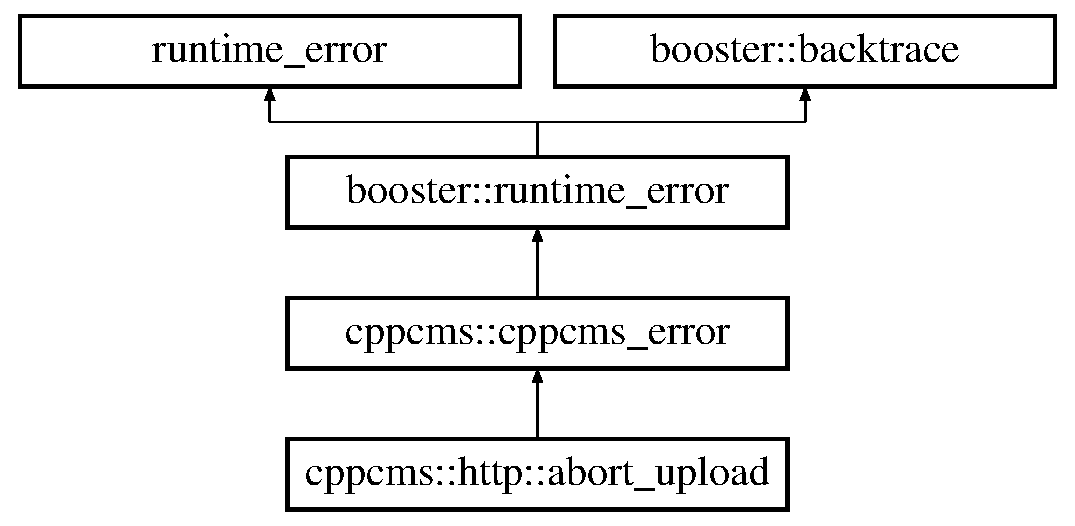
\includegraphics[height=4.000000cm]{classcppcms_1_1http_1_1abort__upload}
\end{center}
\end{figure}
\subsection*{Public Member Functions}
\begin{DoxyCompactItemize}
\item 
{\bf abort\+\_\+upload} (int status\+\_\+code)
\item 
int {\bf code} () const 
\end{DoxyCompactItemize}
\subsection*{Additional Inherited Members}


\subsection{Detailed Description}
Exceptions that is thrown to abort content upload progress indicating an error

\doxyref{New in Cpp\+C\+MS 1.\+2}{p.}{v1_2} 

\subsection{Constructor \& Destructor Documentation}
\index{cppcms\+::http\+::abort\+\_\+upload@{cppcms\+::http\+::abort\+\_\+upload}!abort\+\_\+upload@{abort\+\_\+upload}}
\index{abort\+\_\+upload@{abort\+\_\+upload}!cppcms\+::http\+::abort\+\_\+upload@{cppcms\+::http\+::abort\+\_\+upload}}
\subsubsection[{abort\+\_\+upload(int status\+\_\+code)}]{\setlength{\rightskip}{0pt plus 5cm}cppcms\+::http\+::abort\+\_\+upload\+::abort\+\_\+upload (
\begin{DoxyParamCaption}
\item[{int}]{status\+\_\+code}
\end{DoxyParamCaption}
)}\label{classcppcms_1_1http_1_1abort__upload_ad64c9afa262488ddb4cfd0eeeaf532d0}
Abort upload progress, thrown from classes derived from \doxyref{basic\+\_\+content\+\_\+filter}{p.}{classcppcms_1_1http_1_1basic__content__filter} to abort the upload progress. status\+\_\+code is the H\+T\+TP error code returned, for example 413 requested entity is too large 

\subsection{Member Function Documentation}
\index{cppcms\+::http\+::abort\+\_\+upload@{cppcms\+::http\+::abort\+\_\+upload}!code@{code}}
\index{code@{code}!cppcms\+::http\+::abort\+\_\+upload@{cppcms\+::http\+::abort\+\_\+upload}}
\subsubsection[{code() const }]{\setlength{\rightskip}{0pt plus 5cm}int cppcms\+::http\+::abort\+\_\+upload\+::code (
\begin{DoxyParamCaption}
{}
\end{DoxyParamCaption}
) const}\label{classcppcms_1_1http_1_1abort__upload_ac68ee1af7e706c222af1ea2b2e8dc023}
Get the code 

The documentation for this class was generated from the following file\+:\begin{DoxyCompactItemize}
\item 
cppcms/http\+\_\+content\+\_\+filter.\+h\end{DoxyCompactItemize}

\section{booster\+:\+:locale\+:\+:abstract\+\_\+calendar Class Reference}
\label{classbooster_1_1locale_1_1abstract__calendar}\index{booster\+::locale\+::abstract\+\_\+calendar@{booster\+::locale\+::abstract\+\_\+calendar}}


{\ttfamily \#include $<$booster/booster/locale/date\+\_\+time\+\_\+facet.\+h$>$}

\subsection*{Public Types}
\begin{DoxyCompactItemize}
\item 
enum {\bf value\+\_\+type} \{ \\*
{\bf absolute\+\_\+minimum}, 
{\bf actual\+\_\+minimum}, 
{\bf greatest\+\_\+minimum}, 
{\bf current}, 
\\*
{\bf least\+\_\+maximum}, 
{\bf actual\+\_\+maximum}, 
{\bf absolute\+\_\+maximum}
 \}
\item 
enum {\bf update\+\_\+type} \{ {\bf move}, 
{\bf roll}
 \}
\item 
enum {\bf calendar\+\_\+option\+\_\+type} \{ {\bf is\+\_\+gregorian}, 
{\bf is\+\_\+dst}
 \}
\end{DoxyCompactItemize}
\subsection*{Public Member Functions}
\begin{DoxyCompactItemize}
\item 
virtual {\bf abstract\+\_\+calendar} $\ast$ {\bf clone} () const =0
\item 
virtual void {\bf set\+\_\+value} ({\bf period\+::marks\+::period\+\_\+mark} p, int value)=0
\item 
virtual void {\bf normalize} ()=0
\item 
virtual int {\bf get\+\_\+value} ({\bf period\+::marks\+::period\+\_\+mark} p, {\bf value\+\_\+type} v) const =0
\item 
virtual void {\bf set\+\_\+time} ({\bf posix\+\_\+time} const \&p)=0
\item 
virtual {\bf posix\+\_\+time} {\bf get\+\_\+time} () const =0
\item 
virtual void {\bf set\+\_\+option} ({\bf calendar\+\_\+option\+\_\+type} opt, int v)=0
\item 
virtual int {\bf get\+\_\+option} ({\bf calendar\+\_\+option\+\_\+type} opt) const =0
\item 
virtual void {\bf adjust\+\_\+value} ({\bf period\+::marks\+::period\+\_\+mark} p, {\bf update\+\_\+type} u, int {\bf difference})=0
\item 
virtual int {\bf difference} ({\bf abstract\+\_\+calendar} const $\ast$other, {\bf period\+::marks\+::period\+\_\+mark} p) const =0
\item 
virtual void {\bf set\+\_\+timezone} (std\+::string const \&tz)=0
\item 
virtual std\+::string {\bf get\+\_\+timezone} () const =0
\item 
virtual bool {\bf same} ({\bf abstract\+\_\+calendar} const $\ast$other) const =0
\end{DoxyCompactItemize}


\subsection{Detailed Description}
This class defines generic calendar class, it is used by \doxyref{date\+\_\+time}{p.}{classbooster_1_1locale_1_1date__time} and calendar objects internally. It is less useful for end users, but it is build for localization backend implementation 

\subsection{Member Enumeration Documentation}
\index{booster\+::locale\+::abstract\+\_\+calendar@{booster\+::locale\+::abstract\+\_\+calendar}!calendar\+\_\+option\+\_\+type@{calendar\+\_\+option\+\_\+type}}
\index{calendar\+\_\+option\+\_\+type@{calendar\+\_\+option\+\_\+type}!booster\+::locale\+::abstract\+\_\+calendar@{booster\+::locale\+::abstract\+\_\+calendar}}
\subsubsection[{calendar\+\_\+option\+\_\+type}]{\setlength{\rightskip}{0pt plus 5cm}enum {\bf booster\+::locale\+::abstract\+\_\+calendar\+::calendar\+\_\+option\+\_\+type}}\label{classbooster_1_1locale_1_1abstract__calendar_a3cfa6edf8067e10074565f5576385041}
Information about calendar \begin{Desc}
\item[Enumerator]\par
\begin{description}
\index{is\+\_\+gregorian@{is\+\_\+gregorian}!booster\+::locale\+::abstract\+\_\+calendar@{booster\+::locale\+::abstract\+\_\+calendar}}\index{booster\+::locale\+::abstract\+\_\+calendar@{booster\+::locale\+::abstract\+\_\+calendar}!is\+\_\+gregorian@{is\+\_\+gregorian}}\item[{\em 
is\+\_\+gregorian\label{classbooster_1_1locale_1_1abstract__calendar_a3cfa6edf8067e10074565f5576385041a43893bbb773ee340797bc49057d0df13}
}]Check if the calendar is Gregorian. \index{is\+\_\+dst@{is\+\_\+dst}!booster\+::locale\+::abstract\+\_\+calendar@{booster\+::locale\+::abstract\+\_\+calendar}}\index{booster\+::locale\+::abstract\+\_\+calendar@{booster\+::locale\+::abstract\+\_\+calendar}!is\+\_\+dst@{is\+\_\+dst}}\item[{\em 
is\+\_\+dst\label{classbooster_1_1locale_1_1abstract__calendar_a3cfa6edf8067e10074565f5576385041ab6bc66122a5168089f8bbde2e3a860c7}
}]Check if the current time is in daylight time savings. \end{description}
\end{Desc}
\index{booster\+::locale\+::abstract\+\_\+calendar@{booster\+::locale\+::abstract\+\_\+calendar}!update\+\_\+type@{update\+\_\+type}}
\index{update\+\_\+type@{update\+\_\+type}!booster\+::locale\+::abstract\+\_\+calendar@{booster\+::locale\+::abstract\+\_\+calendar}}
\subsubsection[{update\+\_\+type}]{\setlength{\rightskip}{0pt plus 5cm}enum {\bf booster\+::locale\+::abstract\+\_\+calendar\+::update\+\_\+type}}\label{classbooster_1_1locale_1_1abstract__calendar_aece8b5ccf3031359093c4135cd599bf2}
A way to update the value \begin{Desc}
\item[Enumerator]\par
\begin{description}
\index{move@{move}!booster\+::locale\+::abstract\+\_\+calendar@{booster\+::locale\+::abstract\+\_\+calendar}}\index{booster\+::locale\+::abstract\+\_\+calendar@{booster\+::locale\+::abstract\+\_\+calendar}!move@{move}}\item[{\em 
move\label{classbooster_1_1locale_1_1abstract__calendar_aece8b5ccf3031359093c4135cd599bf2ac8a6abeca668f39831cb560eaeaba76a}
}]Change the value up or down effecting others for example 1990-\/12-\/31 + 1 day = 1991-\/01-\/01. \index{roll@{roll}!booster\+::locale\+::abstract\+\_\+calendar@{booster\+::locale\+::abstract\+\_\+calendar}}\index{booster\+::locale\+::abstract\+\_\+calendar@{booster\+::locale\+::abstract\+\_\+calendar}!roll@{roll}}\item[{\em 
roll\label{classbooster_1_1locale_1_1abstract__calendar_aece8b5ccf3031359093c4135cd599bf2aeb1a59d6ddc5edd62b8599b4c5bdf786}
}]Change the value up or down not effecting others for example 1990-\/12-\/31 + 1 day = 1990-\/12-\/01. \end{description}
\end{Desc}
\index{booster\+::locale\+::abstract\+\_\+calendar@{booster\+::locale\+::abstract\+\_\+calendar}!value\+\_\+type@{value\+\_\+type}}
\index{value\+\_\+type@{value\+\_\+type}!booster\+::locale\+::abstract\+\_\+calendar@{booster\+::locale\+::abstract\+\_\+calendar}}
\subsubsection[{value\+\_\+type}]{\setlength{\rightskip}{0pt plus 5cm}enum {\bf booster\+::locale\+::abstract\+\_\+calendar\+::value\+\_\+type}}\label{classbooster_1_1locale_1_1abstract__calendar_a816ac3e9b4644f56c74654238d55bc00}
Type that defines how to fetch the value \begin{Desc}
\item[Enumerator]\par
\begin{description}
\index{absolute\+\_\+minimum@{absolute\+\_\+minimum}!booster\+::locale\+::abstract\+\_\+calendar@{booster\+::locale\+::abstract\+\_\+calendar}}\index{booster\+::locale\+::abstract\+\_\+calendar@{booster\+::locale\+::abstract\+\_\+calendar}!absolute\+\_\+minimum@{absolute\+\_\+minimum}}\item[{\em 
absolute\+\_\+minimum\label{classbooster_1_1locale_1_1abstract__calendar_a816ac3e9b4644f56c74654238d55bc00a881d2272d3fcb6badc6b9abd54356739}
}]Absolute possible minimum for the value, for example for day is 1. \index{actual\+\_\+minimum@{actual\+\_\+minimum}!booster\+::locale\+::abstract\+\_\+calendar@{booster\+::locale\+::abstract\+\_\+calendar}}\index{booster\+::locale\+::abstract\+\_\+calendar@{booster\+::locale\+::abstract\+\_\+calendar}!actual\+\_\+minimum@{actual\+\_\+minimum}}\item[{\em 
actual\+\_\+minimum\label{classbooster_1_1locale_1_1abstract__calendar_a816ac3e9b4644f56c74654238d55bc00aa6f6b92122288040704a6296bfd49f2a}
}]Actual minimal value for this period. \index{greatest\+\_\+minimum@{greatest\+\_\+minimum}!booster\+::locale\+::abstract\+\_\+calendar@{booster\+::locale\+::abstract\+\_\+calendar}}\index{booster\+::locale\+::abstract\+\_\+calendar@{booster\+::locale\+::abstract\+\_\+calendar}!greatest\+\_\+minimum@{greatest\+\_\+minimum}}\item[{\em 
greatest\+\_\+minimum\label{classbooster_1_1locale_1_1abstract__calendar_a816ac3e9b4644f56c74654238d55bc00aaf1914bf27a3db7bb425d113098b15c2}
}]Maximal minimum value that can be for this period. \index{current@{current}!booster\+::locale\+::abstract\+\_\+calendar@{booster\+::locale\+::abstract\+\_\+calendar}}\index{booster\+::locale\+::abstract\+\_\+calendar@{booster\+::locale\+::abstract\+\_\+calendar}!current@{current}}\item[{\em 
current\label{classbooster_1_1locale_1_1abstract__calendar_a816ac3e9b4644f56c74654238d55bc00a028b3c7c24a63a3ebf4e817e9e3edbda}
}]Current value of this period. \index{least\+\_\+maximum@{least\+\_\+maximum}!booster\+::locale\+::abstract\+\_\+calendar@{booster\+::locale\+::abstract\+\_\+calendar}}\index{booster\+::locale\+::abstract\+\_\+calendar@{booster\+::locale\+::abstract\+\_\+calendar}!least\+\_\+maximum@{least\+\_\+maximum}}\item[{\em 
least\+\_\+maximum\label{classbooster_1_1locale_1_1abstract__calendar_a816ac3e9b4644f56c74654238d55bc00a93375f197a8d4398969e478b01022064}
}]The last maximal value for this period, For example for Gregorian calendar day it is 28 \index{actual\+\_\+maximum@{actual\+\_\+maximum}!booster\+::locale\+::abstract\+\_\+calendar@{booster\+::locale\+::abstract\+\_\+calendar}}\index{booster\+::locale\+::abstract\+\_\+calendar@{booster\+::locale\+::abstract\+\_\+calendar}!actual\+\_\+maximum@{actual\+\_\+maximum}}\item[{\em 
actual\+\_\+maximum\label{classbooster_1_1locale_1_1abstract__calendar_a816ac3e9b4644f56c74654238d55bc00a4bda6b277252cd7f9f1f1cc08c99a550}
}]Actual maximum, for it can be 28, 29, 30, 31 for day according to current month. \index{absolute\+\_\+maximum@{absolute\+\_\+maximum}!booster\+::locale\+::abstract\+\_\+calendar@{booster\+::locale\+::abstract\+\_\+calendar}}\index{booster\+::locale\+::abstract\+\_\+calendar@{booster\+::locale\+::abstract\+\_\+calendar}!absolute\+\_\+maximum@{absolute\+\_\+maximum}}\item[{\em 
absolute\+\_\+maximum\label{classbooster_1_1locale_1_1abstract__calendar_a816ac3e9b4644f56c74654238d55bc00abc0e993c75d2c2b9add870233956a8b2}
}]Maximal value, for Gregorian day it would be 31. \end{description}
\end{Desc}


\subsection{Member Function Documentation}
\index{booster\+::locale\+::abstract\+\_\+calendar@{booster\+::locale\+::abstract\+\_\+calendar}!adjust\+\_\+value@{adjust\+\_\+value}}
\index{adjust\+\_\+value@{adjust\+\_\+value}!booster\+::locale\+::abstract\+\_\+calendar@{booster\+::locale\+::abstract\+\_\+calendar}}
\subsubsection[{adjust\+\_\+value(period\+::marks\+::period\+\_\+mark p, update\+\_\+type u, int difference)=0}]{\setlength{\rightskip}{0pt plus 5cm}virtual void booster\+::locale\+::abstract\+\_\+calendar\+::adjust\+\_\+value (
\begin{DoxyParamCaption}
\item[{{\bf period\+::marks\+::period\+\_\+mark}}]{p, }
\item[{{\bf update\+\_\+type}}]{u, }
\item[{int}]{difference}
\end{DoxyParamCaption}
)\hspace{0.3cm}{\ttfamily [pure virtual]}}\label{classbooster_1_1locale_1_1abstract__calendar_a258f29f26e746c48827b66e58d7675ea}
Adjust period\textquotesingle{}s {\itshape p} value by {\itshape difference} items using a update\+\_\+type {\itshape u}. Note\+: not all values are adjustable \index{booster\+::locale\+::abstract\+\_\+calendar@{booster\+::locale\+::abstract\+\_\+calendar}!clone@{clone}}
\index{clone@{clone}!booster\+::locale\+::abstract\+\_\+calendar@{booster\+::locale\+::abstract\+\_\+calendar}}
\subsubsection[{clone() const =0}]{\setlength{\rightskip}{0pt plus 5cm}virtual {\bf abstract\+\_\+calendar}$\ast$ booster\+::locale\+::abstract\+\_\+calendar\+::clone (
\begin{DoxyParamCaption}
{}
\end{DoxyParamCaption}
) const\hspace{0.3cm}{\ttfamily [pure virtual]}}\label{classbooster_1_1locale_1_1abstract__calendar_a35ded1c475ee09910b6ad78a0c724f28}
Make a polymorphic copy of the calendar \index{booster\+::locale\+::abstract\+\_\+calendar@{booster\+::locale\+::abstract\+\_\+calendar}!difference@{difference}}
\index{difference@{difference}!booster\+::locale\+::abstract\+\_\+calendar@{booster\+::locale\+::abstract\+\_\+calendar}}
\subsubsection[{difference(abstract\+\_\+calendar const $\ast$other, period\+::marks\+::period\+\_\+mark p) const =0}]{\setlength{\rightskip}{0pt plus 5cm}virtual int booster\+::locale\+::abstract\+\_\+calendar\+::difference (
\begin{DoxyParamCaption}
\item[{{\bf abstract\+\_\+calendar} const $\ast$}]{other, }
\item[{{\bf period\+::marks\+::period\+\_\+mark}}]{p}
\end{DoxyParamCaption}
) const\hspace{0.3cm}{\ttfamily [pure virtual]}}\label{classbooster_1_1locale_1_1abstract__calendar_a57121fa4224a48cb54a8caceda8c5942}
Calculate the difference between this calendar and {\itshape other} in {\itshape p} units \index{booster\+::locale\+::abstract\+\_\+calendar@{booster\+::locale\+::abstract\+\_\+calendar}!get\+\_\+option@{get\+\_\+option}}
\index{get\+\_\+option@{get\+\_\+option}!booster\+::locale\+::abstract\+\_\+calendar@{booster\+::locale\+::abstract\+\_\+calendar}}
\subsubsection[{get\+\_\+option(calendar\+\_\+option\+\_\+type opt) const =0}]{\setlength{\rightskip}{0pt plus 5cm}virtual int booster\+::locale\+::abstract\+\_\+calendar\+::get\+\_\+option (
\begin{DoxyParamCaption}
\item[{{\bf calendar\+\_\+option\+\_\+type}}]{opt}
\end{DoxyParamCaption}
) const\hspace{0.3cm}{\ttfamily [pure virtual]}}\label{classbooster_1_1locale_1_1abstract__calendar_a5769c287cdb610a12e2d9d4e959b5f70}
Get option for calendar, currently only check if it is Gregorian calendar \index{booster\+::locale\+::abstract\+\_\+calendar@{booster\+::locale\+::abstract\+\_\+calendar}!get\+\_\+time@{get\+\_\+time}}
\index{get\+\_\+time@{get\+\_\+time}!booster\+::locale\+::abstract\+\_\+calendar@{booster\+::locale\+::abstract\+\_\+calendar}}
\subsubsection[{get\+\_\+time() const =0}]{\setlength{\rightskip}{0pt plus 5cm}virtual {\bf posix\+\_\+time} booster\+::locale\+::abstract\+\_\+calendar\+::get\+\_\+time (
\begin{DoxyParamCaption}
{}
\end{DoxyParamCaption}
) const\hspace{0.3cm}{\ttfamily [pure virtual]}}\label{classbooster_1_1locale_1_1abstract__calendar_a3f02aba2fd6562bc86bb0c495a4a2bb0}
Get current time point \index{booster\+::locale\+::abstract\+\_\+calendar@{booster\+::locale\+::abstract\+\_\+calendar}!get\+\_\+timezone@{get\+\_\+timezone}}
\index{get\+\_\+timezone@{get\+\_\+timezone}!booster\+::locale\+::abstract\+\_\+calendar@{booster\+::locale\+::abstract\+\_\+calendar}}
\subsubsection[{get\+\_\+timezone() const =0}]{\setlength{\rightskip}{0pt plus 5cm}virtual std\+::string booster\+::locale\+::abstract\+\_\+calendar\+::get\+\_\+timezone (
\begin{DoxyParamCaption}
{}
\end{DoxyParamCaption}
) const\hspace{0.3cm}{\ttfamily [pure virtual]}}\label{classbooster_1_1locale_1_1abstract__calendar_ac75b22076cb7cd0ebeea329c00676260}
Get current time zone, empty -\/ system one \index{booster\+::locale\+::abstract\+\_\+calendar@{booster\+::locale\+::abstract\+\_\+calendar}!get\+\_\+value@{get\+\_\+value}}
\index{get\+\_\+value@{get\+\_\+value}!booster\+::locale\+::abstract\+\_\+calendar@{booster\+::locale\+::abstract\+\_\+calendar}}
\subsubsection[{get\+\_\+value(period\+::marks\+::period\+\_\+mark p, value\+\_\+type v) const =0}]{\setlength{\rightskip}{0pt plus 5cm}virtual int booster\+::locale\+::abstract\+\_\+calendar\+::get\+\_\+value (
\begin{DoxyParamCaption}
\item[{{\bf period\+::marks\+::period\+\_\+mark}}]{p, }
\item[{{\bf value\+\_\+type}}]{v}
\end{DoxyParamCaption}
) const\hspace{0.3cm}{\ttfamily [pure virtual]}}\label{classbooster_1_1locale_1_1abstract__calendar_aaf0edf75d8092670d369a1dc95d670c9}
Get specific value for period {\itshape p} according to a value\+\_\+type {\itshape v} \index{booster\+::locale\+::abstract\+\_\+calendar@{booster\+::locale\+::abstract\+\_\+calendar}!normalize@{normalize}}
\index{normalize@{normalize}!booster\+::locale\+::abstract\+\_\+calendar@{booster\+::locale\+::abstract\+\_\+calendar}}
\subsubsection[{normalize()=0}]{\setlength{\rightskip}{0pt plus 5cm}virtual void booster\+::locale\+::abstract\+\_\+calendar\+::normalize (
\begin{DoxyParamCaption}
{}
\end{DoxyParamCaption}
)\hspace{0.3cm}{\ttfamily [pure virtual]}}\label{classbooster_1_1locale_1_1abstract__calendar_ac2bf29d14298154b55ad7aef494c503b}
Recalculate all periods after setting them, should be called after use of \doxyref{set\+\_\+value()}{p.}{classbooster_1_1locale_1_1abstract__calendar_a2c13913b0953e04a4f3264208393751d} function. \index{booster\+::locale\+::abstract\+\_\+calendar@{booster\+::locale\+::abstract\+\_\+calendar}!same@{same}}
\index{same@{same}!booster\+::locale\+::abstract\+\_\+calendar@{booster\+::locale\+::abstract\+\_\+calendar}}
\subsubsection[{same(abstract\+\_\+calendar const $\ast$other) const =0}]{\setlength{\rightskip}{0pt plus 5cm}virtual bool booster\+::locale\+::abstract\+\_\+calendar\+::same (
\begin{DoxyParamCaption}
\item[{{\bf abstract\+\_\+calendar} const $\ast$}]{other}
\end{DoxyParamCaption}
) const\hspace{0.3cm}{\ttfamily [pure virtual]}}\label{classbooster_1_1locale_1_1abstract__calendar_af02d55d84b1a5b0504a7dd17a26ac6c6}
Check of two calendars have same rules \index{booster\+::locale\+::abstract\+\_\+calendar@{booster\+::locale\+::abstract\+\_\+calendar}!set\+\_\+option@{set\+\_\+option}}
\index{set\+\_\+option@{set\+\_\+option}!booster\+::locale\+::abstract\+\_\+calendar@{booster\+::locale\+::abstract\+\_\+calendar}}
\subsubsection[{set\+\_\+option(calendar\+\_\+option\+\_\+type opt, int v)=0}]{\setlength{\rightskip}{0pt plus 5cm}virtual void booster\+::locale\+::abstract\+\_\+calendar\+::set\+\_\+option (
\begin{DoxyParamCaption}
\item[{{\bf calendar\+\_\+option\+\_\+type}}]{opt, }
\item[{int}]{v}
\end{DoxyParamCaption}
)\hspace{0.3cm}{\ttfamily [pure virtual]}}\label{classbooster_1_1locale_1_1abstract__calendar_ae875df81d6bc987b539c7f83a74a1b56}
Set option for calendar, for future use \index{booster\+::locale\+::abstract\+\_\+calendar@{booster\+::locale\+::abstract\+\_\+calendar}!set\+\_\+time@{set\+\_\+time}}
\index{set\+\_\+time@{set\+\_\+time}!booster\+::locale\+::abstract\+\_\+calendar@{booster\+::locale\+::abstract\+\_\+calendar}}
\subsubsection[{set\+\_\+time(posix\+\_\+time const \&p)=0}]{\setlength{\rightskip}{0pt plus 5cm}virtual void booster\+::locale\+::abstract\+\_\+calendar\+::set\+\_\+time (
\begin{DoxyParamCaption}
\item[{{\bf posix\+\_\+time} const \&}]{p}
\end{DoxyParamCaption}
)\hspace{0.3cm}{\ttfamily [pure virtual]}}\label{classbooster_1_1locale_1_1abstract__calendar_ac44ec6740f265aaf109285d95f5fccb9}
Set current time point \index{booster\+::locale\+::abstract\+\_\+calendar@{booster\+::locale\+::abstract\+\_\+calendar}!set\+\_\+timezone@{set\+\_\+timezone}}
\index{set\+\_\+timezone@{set\+\_\+timezone}!booster\+::locale\+::abstract\+\_\+calendar@{booster\+::locale\+::abstract\+\_\+calendar}}
\subsubsection[{set\+\_\+timezone(std\+::string const \&tz)=0}]{\setlength{\rightskip}{0pt plus 5cm}virtual void booster\+::locale\+::abstract\+\_\+calendar\+::set\+\_\+timezone (
\begin{DoxyParamCaption}
\item[{std\+::string const \&}]{tz}
\end{DoxyParamCaption}
)\hspace{0.3cm}{\ttfamily [pure virtual]}}\label{classbooster_1_1locale_1_1abstract__calendar_a9e2fdbaa204f01e4094475785034530a}
Set time zone, empty -\/ use system \index{booster\+::locale\+::abstract\+\_\+calendar@{booster\+::locale\+::abstract\+\_\+calendar}!set\+\_\+value@{set\+\_\+value}}
\index{set\+\_\+value@{set\+\_\+value}!booster\+::locale\+::abstract\+\_\+calendar@{booster\+::locale\+::abstract\+\_\+calendar}}
\subsubsection[{set\+\_\+value(period\+::marks\+::period\+\_\+mark p, int value)=0}]{\setlength{\rightskip}{0pt plus 5cm}virtual void booster\+::locale\+::abstract\+\_\+calendar\+::set\+\_\+value (
\begin{DoxyParamCaption}
\item[{{\bf period\+::marks\+::period\+\_\+mark}}]{p, }
\item[{int}]{value}
\end{DoxyParamCaption}
)\hspace{0.3cm}{\ttfamily [pure virtual]}}\label{classbooster_1_1locale_1_1abstract__calendar_a2c13913b0953e04a4f3264208393751d}
Set specific {\itshape value} for period {\itshape p}, note not all values are settable.

After call of set\+\_\+value you may want to call \doxyref{normalize()}{p.}{classbooster_1_1locale_1_1abstract__calendar_ac2bf29d14298154b55ad7aef494c503b} function to make sure vall periods are updated, if you set sereral fields that are part of single date/time representation you should call set\+\_\+value several times and then call \doxyref{normalize()}{p.}{classbooster_1_1locale_1_1abstract__calendar_ac2bf29d14298154b55ad7aef494c503b}.

If \doxyref{normalize()}{p.}{classbooster_1_1locale_1_1abstract__calendar_ac2bf29d14298154b55ad7aef494c503b} is not called after set\+\_\+value, the behavior is undefined 

The documentation for this class was generated from the following file\+:\begin{DoxyCompactItemize}
\item 
booster/locale/date\+\_\+time\+\_\+facet.\+h\end{DoxyCompactItemize}

\section{booster\+:\+:aio\+:\+:acceptor Class Reference}
\label{classbooster_1_1aio_1_1acceptor}\index{booster\+::aio\+::acceptor@{booster\+::aio\+::acceptor}}


this class represents a socket that accepts incoming connections  




{\ttfamily \#include $<$booster/booster/aio/acceptor.\+h$>$}

Inheritance diagram for booster\+:\+:aio\+:\+:acceptor\+:\begin{figure}[H]
\begin{center}
\leavevmode
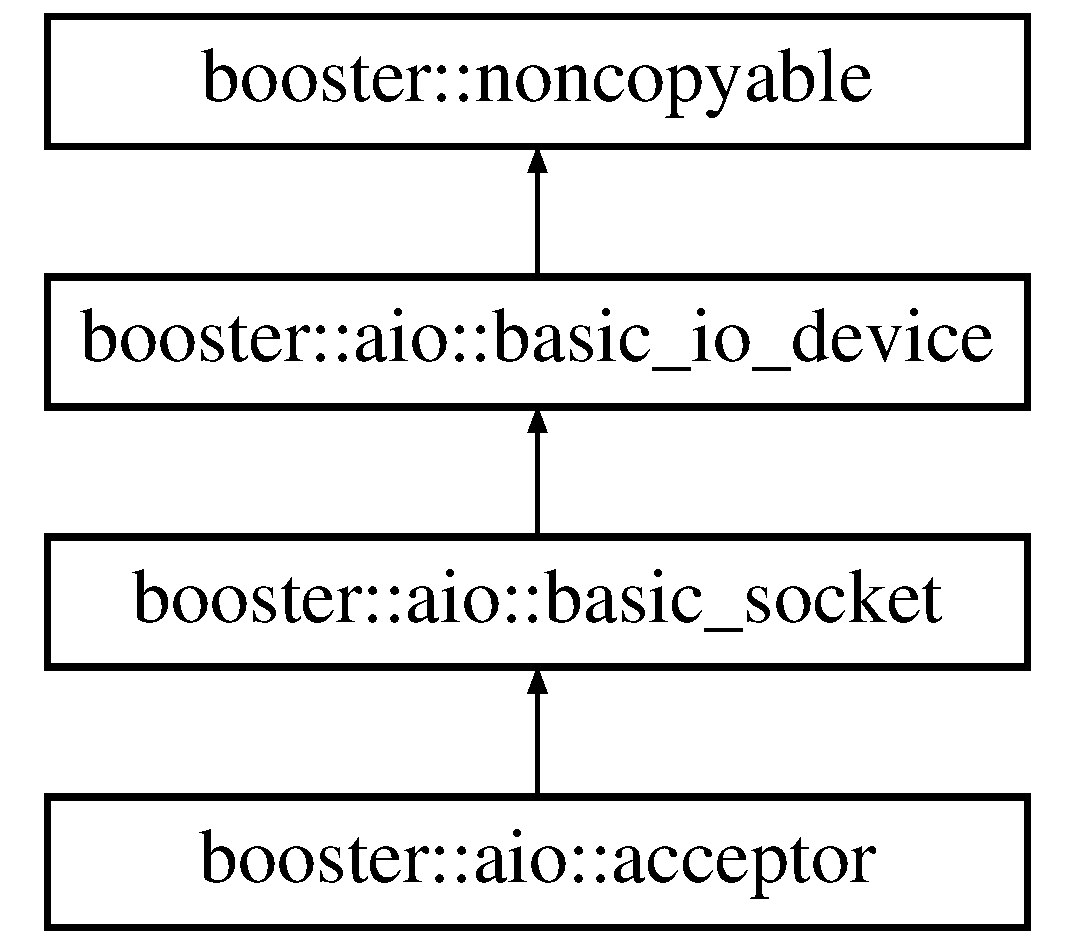
\includegraphics[height=4.000000cm]{classbooster_1_1aio_1_1acceptor}
\end{center}
\end{figure}
\subsection*{Public Member Functions}
\begin{DoxyCompactItemize}
\item 
{\bf acceptor} ()
\item 
{\bf acceptor} ({\bf io\+\_\+service} \&srv)
\item 
void {\bf open} ({\bf family\+\_\+type} d)
\item 
void {\bf open} ({\bf family\+\_\+type} d, system\+::error\+\_\+code \&e)
\item 
void {\bf accept} ({\bf stream\+\_\+socket} \&s)
\item 
void {\bf accept} ({\bf stream\+\_\+socket} \&s, system\+::error\+\_\+code \&e)
\item 
void {\bf bind} ({\bf endpoint} const \&ep)
\item 
void {\bf bind} ({\bf endpoint} const \&ep, system\+::error\+\_\+code \&e)
\item 
void {\bf listen} (int backlog)
\item 
void {\bf listen} (int backlog, system\+::error\+\_\+code \&e)
\item 
void {\bf async\+\_\+accept} ({\bf stream\+\_\+socket} \&s, {\bf event\+\_\+handler} const \&h)
\end{DoxyCompactItemize}
\subsection*{Additional Inherited Members}


\subsection{Detailed Description}
this class represents a socket that accepts incoming connections 

\subsection{Constructor \& Destructor Documentation}
\index{booster\+::aio\+::acceptor@{booster\+::aio\+::acceptor}!acceptor@{acceptor}}
\index{acceptor@{acceptor}!booster\+::aio\+::acceptor@{booster\+::aio\+::acceptor}}
\subsubsection[{acceptor()}]{\setlength{\rightskip}{0pt plus 5cm}booster\+::aio\+::acceptor\+::acceptor (
\begin{DoxyParamCaption}
{}
\end{DoxyParamCaption}
)}\label{classbooster_1_1aio_1_1acceptor_ac28c6165bed8d65f9db932c5a65d9909}
Create a new acceptor object \index{booster\+::aio\+::acceptor@{booster\+::aio\+::acceptor}!acceptor@{acceptor}}
\index{acceptor@{acceptor}!booster\+::aio\+::acceptor@{booster\+::aio\+::acceptor}}
\subsubsection[{acceptor(io\+\_\+service \&srv)}]{\setlength{\rightskip}{0pt plus 5cm}booster\+::aio\+::acceptor\+::acceptor (
\begin{DoxyParamCaption}
\item[{{\bf io\+\_\+service} \&}]{srv}
\end{DoxyParamCaption}
)}\label{classbooster_1_1aio_1_1acceptor_af6c68d8cbfb59da3579b3cbbb0b21b8a}
Create a new acceptor object with assigned \doxyref{io\+\_\+service}{p.}{classbooster_1_1aio_1_1io__service} {\itshape srv}) 

\subsection{Member Function Documentation}
\index{booster\+::aio\+::acceptor@{booster\+::aio\+::acceptor}!accept@{accept}}
\index{accept@{accept}!booster\+::aio\+::acceptor@{booster\+::aio\+::acceptor}}
\subsubsection[{accept(stream\+\_\+socket \&s)}]{\setlength{\rightskip}{0pt plus 5cm}void booster\+::aio\+::acceptor\+::accept (
\begin{DoxyParamCaption}
\item[{{\bf stream\+\_\+socket} \&}]{s}
\end{DoxyParamCaption}
)}\label{classbooster_1_1aio_1_1acceptor_aebf231cf0aa40375984830cb2627f249}
Accepts a new incoming connection to the socket {\itshape s} 

Throws system\+::system\+\_\+error if error occurs. \index{booster\+::aio\+::acceptor@{booster\+::aio\+::acceptor}!accept@{accept}}
\index{accept@{accept}!booster\+::aio\+::acceptor@{booster\+::aio\+::acceptor}}
\subsubsection[{accept(stream\+\_\+socket \&s, system\+::error\+\_\+code \&e)}]{\setlength{\rightskip}{0pt plus 5cm}void booster\+::aio\+::acceptor\+::accept (
\begin{DoxyParamCaption}
\item[{{\bf stream\+\_\+socket} \&}]{s, }
\item[{system\+::error\+\_\+code \&}]{e}
\end{DoxyParamCaption}
)}\label{classbooster_1_1aio_1_1acceptor_a151ca53f90616d2f96e15c35017ea0e9}
Accepts a new incoming connection to the socket {\itshape s} 

If a error occurs it is assigned to {\itshape e}. \index{booster\+::aio\+::acceptor@{booster\+::aio\+::acceptor}!async\+\_\+accept@{async\+\_\+accept}}
\index{async\+\_\+accept@{async\+\_\+accept}!booster\+::aio\+::acceptor@{booster\+::aio\+::acceptor}}
\subsubsection[{async\+\_\+accept(stream\+\_\+socket \&s, event\+\_\+handler const \&h)}]{\setlength{\rightskip}{0pt plus 5cm}void booster\+::aio\+::acceptor\+::async\+\_\+accept (
\begin{DoxyParamCaption}
\item[{{\bf stream\+\_\+socket} \&}]{s, }
\item[{{\bf event\+\_\+handler} const \&}]{h}
\end{DoxyParamCaption}
)}\label{classbooster_1_1aio_1_1acceptor_a3cddf6da3919067e25c3d39e39381a58}
Accept the connection asynchronously. The reference {\itshape s} must be valid until h is called.

If \doxyref{io\+\_\+service}{p.}{classbooster_1_1aio_1_1io__service} is not assigned throws system\+::system\+\_\+error, all other errors reported via the callback {\itshape h}. \index{booster\+::aio\+::acceptor@{booster\+::aio\+::acceptor}!bind@{bind}}
\index{bind@{bind}!booster\+::aio\+::acceptor@{booster\+::aio\+::acceptor}}
\subsubsection[{bind(endpoint const \&ep)}]{\setlength{\rightskip}{0pt plus 5cm}void booster\+::aio\+::acceptor\+::bind (
\begin{DoxyParamCaption}
\item[{{\bf endpoint} const \&}]{ep}
\end{DoxyParamCaption}
)}\label{classbooster_1_1aio_1_1acceptor_ac80b06a28bc8d2ec76134fa4d3b52c53}
Bind the opended socket the \doxyref{endpoint}{p.}{classbooster_1_1aio_1_1endpoint} {\itshape ep} 

Throws system\+::system\+\_\+error if error occurs.

Note\+: calls basic\+\_\+socket\+::bind(ep) -\/ exists there just for backward compatibility \index{booster\+::aio\+::acceptor@{booster\+::aio\+::acceptor}!bind@{bind}}
\index{bind@{bind}!booster\+::aio\+::acceptor@{booster\+::aio\+::acceptor}}
\subsubsection[{bind(endpoint const \&ep, system\+::error\+\_\+code \&e)}]{\setlength{\rightskip}{0pt plus 5cm}void booster\+::aio\+::acceptor\+::bind (
\begin{DoxyParamCaption}
\item[{{\bf endpoint} const \&}]{ep, }
\item[{system\+::error\+\_\+code \&}]{e}
\end{DoxyParamCaption}
)}\label{classbooster_1_1aio_1_1acceptor_a20bd5aa0a450945fa0cca580b0ca540b}
Bind the opended socket the \doxyref{endpoint}{p.}{classbooster_1_1aio_1_1endpoint} {\itshape ep} 

If a error occurs it is assigned to {\itshape e}.

Note\+: calls basic\+\_\+socket\+::bind(ep,e) -\/ exists there just for backward compatibility \index{booster\+::aio\+::acceptor@{booster\+::aio\+::acceptor}!listen@{listen}}
\index{listen@{listen}!booster\+::aio\+::acceptor@{booster\+::aio\+::acceptor}}
\subsubsection[{listen(int backlog)}]{\setlength{\rightskip}{0pt plus 5cm}void booster\+::aio\+::acceptor\+::listen (
\begin{DoxyParamCaption}
\item[{int}]{backlog}
\end{DoxyParamCaption}
)}\label{classbooster_1_1aio_1_1acceptor_abb92e6f71d3147ec154f68a63d0fc0bc}
Starts listening on the socket with backlog parameter {\itshape backlog} 

Throws system\+::system\+\_\+error if error occurs. \index{booster\+::aio\+::acceptor@{booster\+::aio\+::acceptor}!listen@{listen}}
\index{listen@{listen}!booster\+::aio\+::acceptor@{booster\+::aio\+::acceptor}}
\subsubsection[{listen(int backlog, system\+::error\+\_\+code \&e)}]{\setlength{\rightskip}{0pt plus 5cm}void booster\+::aio\+::acceptor\+::listen (
\begin{DoxyParamCaption}
\item[{int}]{backlog, }
\item[{system\+::error\+\_\+code \&}]{e}
\end{DoxyParamCaption}
)}\label{classbooster_1_1aio_1_1acceptor_a763dc1e68e4e83b574c7bec08687c770}
Starts listening on the socket with backlog parameter {\itshape backlog} 

If a error occurs it is assigned to {\itshape e}. \index{booster\+::aio\+::acceptor@{booster\+::aio\+::acceptor}!open@{open}}
\index{open@{open}!booster\+::aio\+::acceptor@{booster\+::aio\+::acceptor}}
\subsubsection[{open(family\+\_\+type d)}]{\setlength{\rightskip}{0pt plus 5cm}void booster\+::aio\+::acceptor\+::open (
\begin{DoxyParamCaption}
\item[{{\bf family\+\_\+type}}]{d}
\end{DoxyParamCaption}
)}\label{classbooster_1_1aio_1_1acceptor_a6859beda7cbd58a13d33238142cc381c}
Opens a new stream socket of a \doxyref{family\+\_\+type}{p.}{namespacebooster_1_1aio_a272e1f9b8b2b4e0cf3289749cd51baaa} {\itshape d} 

Throws system\+::system\+\_\+error if error occurs. \index{booster\+::aio\+::acceptor@{booster\+::aio\+::acceptor}!open@{open}}
\index{open@{open}!booster\+::aio\+::acceptor@{booster\+::aio\+::acceptor}}
\subsubsection[{open(family\+\_\+type d, system\+::error\+\_\+code \&e)}]{\setlength{\rightskip}{0pt plus 5cm}void booster\+::aio\+::acceptor\+::open (
\begin{DoxyParamCaption}
\item[{{\bf family\+\_\+type}}]{d, }
\item[{system\+::error\+\_\+code \&}]{e}
\end{DoxyParamCaption}
)}\label{classbooster_1_1aio_1_1acceptor_aa15b6d876aaded5bb2a4c46e67ebb974}
Opens a new stream socket of a \doxyref{family\+\_\+type}{p.}{namespacebooster_1_1aio_a272e1f9b8b2b4e0cf3289749cd51baaa} {\itshape d} 

If a error occurs it is assigned to {\itshape e}. 

The documentation for this class was generated from the following file\+:\begin{DoxyCompactItemize}
\item 
booster/aio/acceptor.\+h\end{DoxyCompactItemize}

\section{cppcms\+:\+:base\+\_\+content\+:\+:app\+\_\+guard Class Reference}
\label{classcppcms_1_1base__content_1_1app__guard}\index{cppcms\+::base\+\_\+content\+::app\+\_\+guard@{cppcms\+::base\+\_\+content\+::app\+\_\+guard}}


Special guard class that allows setting and resetting content\textquotesingle{}s rendeding according to the specific scope.  




{\ttfamily \#include $<$cppcms/base\+\_\+content.\+h$>$}

\subsection*{Public Member Functions}
\begin{DoxyCompactItemize}
\item 
{\bf app\+\_\+guard} ({\bf base\+\_\+content} \&c, {\bf application} \&a)
\item 
{\bf app\+\_\+guard} ({\bf base\+\_\+content} \&c, {\bf base\+\_\+content} \&parent)
\item 
{\bf $\sim$app\+\_\+guard} ()
\end{DoxyCompactItemize}


\subsection{Detailed Description}
Special guard class that allows setting and resetting content\textquotesingle{}s rendeding according to the specific scope. 

\subsection{Constructor \& Destructor Documentation}
\index{cppcms\+::base\+\_\+content\+::app\+\_\+guard@{cppcms\+::base\+\_\+content\+::app\+\_\+guard}!app\+\_\+guard@{app\+\_\+guard}}
\index{app\+\_\+guard@{app\+\_\+guard}!cppcms\+::base\+\_\+content\+::app\+\_\+guard@{cppcms\+::base\+\_\+content\+::app\+\_\+guard}}
\subsubsection[{app\+\_\+guard(base\+\_\+content \&c, application \&a)}]{\setlength{\rightskip}{0pt plus 5cm}cppcms\+::base\+\_\+content\+::app\+\_\+guard\+::app\+\_\+guard (
\begin{DoxyParamCaption}
\item[{{\bf base\+\_\+content} \&}]{c, }
\item[{{\bf application} \&}]{a}
\end{DoxyParamCaption}
)\hspace{0.3cm}{\ttfamily [inline]}}\label{classcppcms_1_1base__content_1_1app__guard_aa4291a024905c14dee1b6f81f433ceb4}
Initialize set the applicaton {\itshape to} a content {\itshape c} if have not one ready 

References cppcms\+::base\+\_\+content\+::app(), and cppcms\+::base\+\_\+content\+::has\+\_\+app().

\index{cppcms\+::base\+\_\+content\+::app\+\_\+guard@{cppcms\+::base\+\_\+content\+::app\+\_\+guard}!app\+\_\+guard@{app\+\_\+guard}}
\index{app\+\_\+guard@{app\+\_\+guard}!cppcms\+::base\+\_\+content\+::app\+\_\+guard@{cppcms\+::base\+\_\+content\+::app\+\_\+guard}}
\subsubsection[{app\+\_\+guard(base\+\_\+content \&c, base\+\_\+content \&parent)}]{\setlength{\rightskip}{0pt plus 5cm}cppcms\+::base\+\_\+content\+::app\+\_\+guard\+::app\+\_\+guard (
\begin{DoxyParamCaption}
\item[{{\bf base\+\_\+content} \&}]{c, }
\item[{{\bf base\+\_\+content} \&}]{parent}
\end{DoxyParamCaption}
)\hspace{0.3cm}{\ttfamily [inline]}}\label{classcppcms_1_1base__content_1_1app__guard_a74de13a3a8e77db44307e520ac2a72ed}
Assign the application to {\itshape c} from the {\itshape parent\textquotesingle{}s} application.

It is assigned if it is not already defined 

References cppcms\+::base\+\_\+content\+::app(), and cppcms\+::base\+\_\+content\+::has\+\_\+app().

\index{cppcms\+::base\+\_\+content\+::app\+\_\+guard@{cppcms\+::base\+\_\+content\+::app\+\_\+guard}!````~app\+\_\+guard@{$\sim$app\+\_\+guard}}
\index{````~app\+\_\+guard@{$\sim$app\+\_\+guard}!cppcms\+::base\+\_\+content\+::app\+\_\+guard@{cppcms\+::base\+\_\+content\+::app\+\_\+guard}}
\subsubsection[{$\sim$app\+\_\+guard()}]{\setlength{\rightskip}{0pt plus 5cm}cppcms\+::base\+\_\+content\+::app\+\_\+guard\+::$\sim$app\+\_\+guard (
\begin{DoxyParamCaption}
{}
\end{DoxyParamCaption}
)\hspace{0.3cm}{\ttfamily [inline]}}\label{classcppcms_1_1base__content_1_1app__guard_a561d78a9495c08b6dbe2bbe4b23678e6}
Reset the application if the content if it was assigned in constructor 

The documentation for this class was generated from the following file\+:\begin{DoxyCompactItemize}
\item 
cppcms/base\+\_\+content.\+h\end{DoxyCompactItemize}

\section{cppcms\+:\+:application Class Reference}
\label{classcppcms_1_1application}\index{cppcms\+::application@{cppcms\+::application}}


application class is the base class for all user created applications.  




{\ttfamily \#include $<$cppcms/application.\+h$>$}

Inheritance diagram for cppcms\+:\+:application\+:\begin{figure}[H]
\begin{center}
\leavevmode
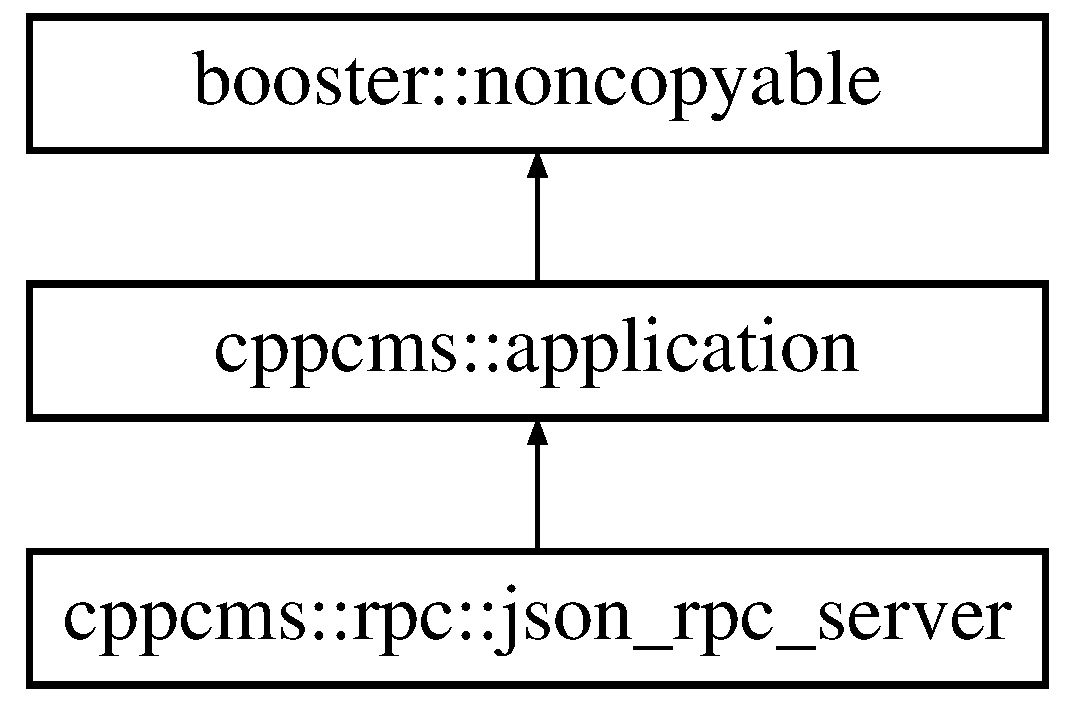
\includegraphics[height=3.000000cm]{classcppcms_1_1application}
\end{center}
\end{figure}
\subsection*{Public Member Functions}
\begin{DoxyCompactItemize}
\item 
{\bf application} ({\bf cppcms\+::service} \&srv)
\item 
virtual {\bf $\sim$application} ()
\item 
{\bf cppcms\+::service} \& {\bf service} ()
\item 
{\bf json\+::value} const \& {\bf settings} ()
\item 
{\bf http\+::context} \& {\bf context} ()
\item 
{\bf http\+::request} \& {\bf request} ()
\item 
{\bf http\+::response} \& {\bf response} ()
\item 
{\bf url\+\_\+dispatcher} \& {\bf dispatcher} ()
\item 
{\bf url\+\_\+mapper} \& {\bf mapper} ()
\item 
{\bf cache\+\_\+interface} \& {\bf cache} ()
\item 
{\bf session\+\_\+interface} \& {\bf session} ()
\item 
void {\bf render} (std\+::string template\+\_\+name, {\bf base\+\_\+content} \&content)
\item 
void {\bf render} (std\+::string skin, std\+::string template\+\_\+name, {\bf base\+\_\+content} \&content)
\item 
void {\bf render} (std\+::string template\+\_\+name, std\+::ostream \&out, {\bf base\+\_\+content} \&content)
\item 
void {\bf render} (std\+::string skin, std\+::string template\+\_\+name, std\+::ostream \&out, {\bf base\+\_\+content} \&content)
\item 
void {\bf add} ({\bf application} \&app)
\item 
void {\bf add} ({\bf application} \&app, std\+::string const \&regex, int part)
\item 
void {\bf add} ({\bf application} \&app, std\+::string const \&name, std\+::string const \&{\bf url}, std\+::string const \&regex, int part)
\item 
void {\bf add} ({\bf application} \&app, std\+::string const \&name, std\+::string const \&{\bf url})
\item 
void {\bf attach} ({\bf application} $\ast$app)
\item 
void {\bf attach} ({\bf application} $\ast$app, std\+::string const \&regex, int part)
\item 
void {\bf attach} ({\bf application} $\ast$app, std\+::string const \&name, std\+::string const \&{\bf url})
\item 
void {\bf attach} ({\bf application} $\ast$app, std\+::string const \&name, std\+::string const \&{\bf url}, std\+::string const \&regex, int part)
\item 
{\bf application} $\ast$ {\bf parent} ()
\item 
{\bf application} $\ast$ {\bf root} ()
\item 
booster\+::shared\+\_\+ptr$<$ {\bf http\+::context} $>$ {\bf release\+\_\+context} ()
\item 
booster\+::shared\+\_\+ptr$<$ {\bf http\+::context} $>$ {\bf get\+\_\+context} ()
\item 
void {\bf assign\+\_\+context} (booster\+::shared\+\_\+ptr$<$ {\bf http\+::context} $>$ conn)
\item 
void {\bf add\+\_\+context} ({\bf http\+::context} \&conn)
\item 
void {\bf remove\+\_\+context} ()
\item 
bool {\bf is\+\_\+asynchronous} ()
\item 
bool {\bf has\+\_\+context} ()
\item 
bool {\bf owns\+\_\+context} ()
\item 
virtual void {\bf main} (std\+::string {\bf url})
\item 
virtual void {\bf init} ()
\item 
virtual void {\bf clear} ()
\item 
std\+::string {\bf translate} (char const $\ast${\bf context}, char const $\ast$message)
\item 
std\+::string {\bf translate} (char const $\ast$message)
\item 
std\+::string {\bf translate} (char const $\ast${\bf context}, char const $\ast$single, char const $\ast$plural, int n)
\item 
std\+::string {\bf translate} (char const $\ast$single, char const $\ast$plural, int n)
\item 
std\+::string {\bf url} (std\+::string const \&key)
\item 
std\+::string {\bf url} (std\+::string const \&key, {\bf filters\+::streamable} const \&p1)
\item 
std\+::string {\bf url} (std\+::string const \&key, {\bf filters\+::streamable} const \&p1, {\bf filters\+::streamable} const \&p2)
\item 
std\+::string {\bf url} (std\+::string const \&key, {\bf filters\+::streamable} const \&p1, {\bf filters\+::streamable} const \&p2, {\bf filters\+::streamable} const \&p3)
\item 
std\+::string {\bf url} (std\+::string const \&key, {\bf filters\+::streamable} const \&p1, {\bf filters\+::streamable} const \&p2, {\bf filters\+::streamable} const \&p3, {\bf filters\+::streamable} const \&p4)
\item 
std\+::string {\bf url} (std\+::string const \&key, {\bf filters\+::streamable} const \&p1, {\bf filters\+::streamable} const \&p2, {\bf filters\+::streamable} const \&p3, {\bf filters\+::streamable} const \&p4, {\bf filters\+::streamable} const \&p5)
\item 
std\+::string {\bf url} (std\+::string const \&key, {\bf filters\+::streamable} const \&p1, {\bf filters\+::streamable} const \&p2, {\bf filters\+::streamable} const \&p3, {\bf filters\+::streamable} const \&p4, {\bf filters\+::streamable} const \&p5, {\bf filters\+::streamable} const \&p6)
\end{DoxyCompactItemize}
\subsection*{Friends}
\begin{DoxyCompactItemize}
\item 
class {\bfseries applications\+\_\+pool}\label{classcppcms_1_1application_a30f874a0e0276d427a1e284dc94255fc}

\item 
class {\bfseries application\+\_\+specific\+\_\+pool}\label{classcppcms_1_1application_a64a5512fc00037c78cc11ab7f955c8e6}

\item 
void {\bfseries booster\+::intrusive\+\_\+ptr\+\_\+add\+\_\+ref} ({\bf application} $\ast$p)\label{classcppcms_1_1application_a50711b8cb60f6581fa5330de7c7f9a59}

\item 
void {\bfseries booster\+::intrusive\+\_\+ptr\+\_\+release} ({\bf application} $\ast$p)\label{classcppcms_1_1application_a089c8bd8e37fe23e20b1f3d4b8a7e080}

\end{DoxyCompactItemize}


\subsection{Detailed Description}
application class is the base class for all user created applications. 

This class is the base for all user actions required for web page generation. User application classes are created upon web page request and then cached in {\itshape application\+\_\+pool}.

Applications can be bundled to hierarchies. You may add a sub application to hierarchy, and they will always be connected with topmost application and their lifetime would be binded to them.

application class is reference counted and may be used with {\itshape intrusive\+\_\+ptr}. But reference count semantics is very different form an ordinary semantics for other classes derived from {\itshape cppcms\+::refcounted}.


\begin{DoxyEnumerate}
\item All hierarchy share the counter of the topmost application. Thus, when all bundle is counted as a single unit allowing passing intrusive\+\_\+ptr to itself to the central service safely. When the topmost application is destroyed, it destroys all its children application classes.
\item When reference count goes to 0, the application is not destroyed but rather recycled to the application pool for future use.
\item The above hold only for synchronous applications, asynchronous one are destroyed when all reference count goes to 0.
\end{DoxyEnumerate}

There two ways to add sub-\/applications to hierarchy\+:


\begin{DoxyEnumerate}
\item Using member function family {\itshape add}, usually used with direct members of the parent class. Such child are not destroyed explicitly.
\item Using member function family {\itshape attach}. The ownership on the application is moved to the parent class and it destroys an attached class with delete. 
\end{DoxyEnumerate}

\subsection{Constructor \& Destructor Documentation}
\index{cppcms\+::application@{cppcms\+::application}!application@{application}}
\index{application@{application}!cppcms\+::application@{cppcms\+::application}}
\subsubsection[{application(cppcms\+::service \&srv)}]{\setlength{\rightskip}{0pt plus 5cm}cppcms\+::application\+::application (
\begin{DoxyParamCaption}
\item[{{\bf cppcms\+::service} \&}]{srv}
\end{DoxyParamCaption}
)}\label{classcppcms_1_1application_af7ea30dd5b894bbe194eb644ee5f9b80}
Create a new application running on service {\itshape srv}, with a parent {\itshape parent} \index{cppcms\+::application@{cppcms\+::application}!````~application@{$\sim$application}}
\index{````~application@{$\sim$application}!cppcms\+::application@{cppcms\+::application}}
\subsubsection[{$\sim$application()}]{\setlength{\rightskip}{0pt plus 5cm}virtual cppcms\+::application\+::$\sim$application (
\begin{DoxyParamCaption}
{}
\end{DoxyParamCaption}
)\hspace{0.3cm}{\ttfamily [virtual]}}\label{classcppcms_1_1application_a1345754d889871fe130aec26f4399afe}
Destroys an application and all assigned application children. 

\subsection{Member Function Documentation}
\index{cppcms\+::application@{cppcms\+::application}!add@{add}}
\index{add@{add}!cppcms\+::application@{cppcms\+::application}}
\subsubsection[{add(application \&app)}]{\setlength{\rightskip}{0pt plus 5cm}void cppcms\+::application\+::add (
\begin{DoxyParamCaption}
\item[{{\bf application} \&}]{app}
\end{DoxyParamCaption}
)}\label{classcppcms_1_1application_afc8693d6a8f20fc21a9141d2f377c2f9}
Register an application {\itshape app} as child. Ownership of app is not transfered to parent, however it would shared it\textquotesingle{}s parent reference count. \index{cppcms\+::application@{cppcms\+::application}!add@{add}}
\index{add@{add}!cppcms\+::application@{cppcms\+::application}}
\subsubsection[{add(application \&app, std\+::string const \&regex, int part)}]{\setlength{\rightskip}{0pt plus 5cm}void cppcms\+::application\+::add (
\begin{DoxyParamCaption}
\item[{{\bf application} \&}]{app, }
\item[{std\+::string const \&}]{regex, }
\item[{int}]{part}
\end{DoxyParamCaption}
)}\label{classcppcms_1_1application_a33ac6e2c219e9b619986f339e64694f9}
Register an application {\itshape app} as child and mount it into url dispatched calling \doxyref{dispatcher()}{p.}{classcppcms_1_1application_aec990ef8b6799f1758447d812feada33}.mount(regex,app,part);

Ownership of app is not transfered to parent, however it would shared it\textquotesingle{}s parent reference count. \index{cppcms\+::application@{cppcms\+::application}!add@{add}}
\index{add@{add}!cppcms\+::application@{cppcms\+::application}}
\subsubsection[{add(application \&app, std\+::string const \&name, std\+::string const \&url, std\+::string const \&regex, int part)}]{\setlength{\rightskip}{0pt plus 5cm}void cppcms\+::application\+::add (
\begin{DoxyParamCaption}
\item[{{\bf application} \&}]{app, }
\item[{std\+::string const \&}]{name, }
\item[{std\+::string const \&}]{url, }
\item[{std\+::string const \&}]{regex, }
\item[{int}]{part}
\end{DoxyParamCaption}
)}\label{classcppcms_1_1application_acd1c5660860aa6ba87987577950b290a}
Register an application {\itshape app} as child and mount it into\+:


\begin{DoxyItemize}
\item \doxyref{url\+\_\+dispatcher}{p.}{classcppcms_1_1url__dispatcher} calling \doxyref{dispatcher()}{p.}{classcppcms_1_1application_aec990ef8b6799f1758447d812feada33}.mount(regex,app,part);
\item \doxyref{url\+\_\+mapper}{p.}{classcppcms_1_1url__mapper} calling \doxyref{mapper()}{p.}{classcppcms_1_1application_a146c62da586922ee00d2af89efc2614f}.mount(name,url,app);

Ownership of app is not transfered to parent, however it would shared it\textquotesingle{}s parent reference count. 
\end{DoxyItemize}\index{cppcms\+::application@{cppcms\+::application}!add@{add}}
\index{add@{add}!cppcms\+::application@{cppcms\+::application}}
\subsubsection[{add(application \&app, std\+::string const \&name, std\+::string const \&url)}]{\setlength{\rightskip}{0pt plus 5cm}void cppcms\+::application\+::add (
\begin{DoxyParamCaption}
\item[{{\bf application} \&}]{app, }
\item[{std\+::string const \&}]{name, }
\item[{std\+::string const \&}]{url}
\end{DoxyParamCaption}
)}\label{classcppcms_1_1application_a7152d901ee841424ddd513eb45053e7f}
Register an application {\itshape app} as child and mount it into \doxyref{url\+\_\+mapper}{p.}{classcppcms_1_1url__mapper} calling \doxyref{mapper()}{p.}{classcppcms_1_1application_a146c62da586922ee00d2af89efc2614f}.mount(name,url,app);

Ownership of app is not transfered to parent, however it would shared it\textquotesingle{}s parent reference count. \index{cppcms\+::application@{cppcms\+::application}!add\+\_\+context@{add\+\_\+context}}
\index{add\+\_\+context@{add\+\_\+context}!cppcms\+::application@{cppcms\+::application}}
\subsubsection[{add\+\_\+context(http\+::context \&conn)}]{\setlength{\rightskip}{0pt plus 5cm}void cppcms\+::application\+::add\+\_\+context (
\begin{DoxyParamCaption}
\item[{{\bf http\+::context} \&}]{conn}
\end{DoxyParamCaption}
)}\label{classcppcms_1_1application_a6bea3b5f42f00e4681d1bf54b4928fef}
Add context to applications such that context ownership isn\textquotesingle{}t transferred to the application

\doxyref{New in Cpp\+C\+MS 1.\+2}{p.}{v1_2} \index{cppcms\+::application@{cppcms\+::application}!assign\+\_\+context@{assign\+\_\+context}}
\index{assign\+\_\+context@{assign\+\_\+context}!cppcms\+::application@{cppcms\+::application}}
\subsubsection[{assign\+\_\+context(booster\+::shared\+\_\+ptr$<$ http\+::context $>$ conn)}]{\setlength{\rightskip}{0pt plus 5cm}void cppcms\+::application\+::assign\+\_\+context (
\begin{DoxyParamCaption}
\item[{booster\+::shared\+\_\+ptr$<$ {\bf http\+::context} $>$}]{conn}
\end{DoxyParamCaption}
)}\label{classcppcms_1_1application_ac87a8ae7d0e15a21850c722c8fe781b3}
Set context to the application. The application gets shared ownership on the context.

Note\+: because application hierarchy shared same context, it affects all classes in it. \index{cppcms\+::application@{cppcms\+::application}!attach@{attach}}
\index{attach@{attach}!cppcms\+::application@{cppcms\+::application}}
\subsubsection[{attach(application $\ast$app)}]{\setlength{\rightskip}{0pt plus 5cm}void cppcms\+::application\+::attach (
\begin{DoxyParamCaption}
\item[{{\bf application} $\ast$}]{app}
\end{DoxyParamCaption}
)}\label{classcppcms_1_1application_a6bf61f58b723d3dc93bdd144c1b0b45b}
Register an application {\itshape app} as child. Ownership of app is transfered to parent \index{cppcms\+::application@{cppcms\+::application}!attach@{attach}}
\index{attach@{attach}!cppcms\+::application@{cppcms\+::application}}
\subsubsection[{attach(application $\ast$app, std\+::string const \&regex, int part)}]{\setlength{\rightskip}{0pt plus 5cm}void cppcms\+::application\+::attach (
\begin{DoxyParamCaption}
\item[{{\bf application} $\ast$}]{app, }
\item[{std\+::string const \&}]{regex, }
\item[{int}]{part}
\end{DoxyParamCaption}
)}\label{classcppcms_1_1application_ab69de715e0871a5a96c9c88145bb4629}
Register an application {\itshape app} as child and mount it into \doxyref{url\+\_\+dispatcher}{p.}{classcppcms_1_1url__dispatcher} calling \doxyref{dispatcher()}{p.}{classcppcms_1_1application_aec990ef8b6799f1758447d812feada33}.mount(regex,$\ast$app,part);

Ownership of app is transfered to parent. \index{cppcms\+::application@{cppcms\+::application}!attach@{attach}}
\index{attach@{attach}!cppcms\+::application@{cppcms\+::application}}
\subsubsection[{attach(application $\ast$app, std\+::string const \&name, std\+::string const \&url)}]{\setlength{\rightskip}{0pt plus 5cm}void cppcms\+::application\+::attach (
\begin{DoxyParamCaption}
\item[{{\bf application} $\ast$}]{app, }
\item[{std\+::string const \&}]{name, }
\item[{std\+::string const \&}]{url}
\end{DoxyParamCaption}
)}\label{classcppcms_1_1application_ab31985c608cfb176bbbf0958f438fbf7}
Register an application {\itshape app} as child and mount it into \doxyref{url\+\_\+mapper}{p.}{classcppcms_1_1url__mapper} calling \doxyref{mapper()}{p.}{classcppcms_1_1application_a146c62da586922ee00d2af89efc2614f}.mount(name,url,$\ast$app);

Ownership of app is transfered to parent. \index{cppcms\+::application@{cppcms\+::application}!attach@{attach}}
\index{attach@{attach}!cppcms\+::application@{cppcms\+::application}}
\subsubsection[{attach(application $\ast$app, std\+::string const \&name, std\+::string const \&url, std\+::string const \&regex, int part)}]{\setlength{\rightskip}{0pt plus 5cm}void cppcms\+::application\+::attach (
\begin{DoxyParamCaption}
\item[{{\bf application} $\ast$}]{app, }
\item[{std\+::string const \&}]{name, }
\item[{std\+::string const \&}]{url, }
\item[{std\+::string const \&}]{regex, }
\item[{int}]{part}
\end{DoxyParamCaption}
)}\label{classcppcms_1_1application_ac9a8c01d43c5364ed1cb6b1fb517ef33}
Register an application {\itshape app} as child and mount it into\+:


\begin{DoxyItemize}
\item \doxyref{url\+\_\+dispatcher}{p.}{classcppcms_1_1url__dispatcher} calling \doxyref{dispatcher()}{p.}{classcppcms_1_1application_aec990ef8b6799f1758447d812feada33}.mount(regex,$\ast$app,part);
\item \doxyref{url\+\_\+mapper}{p.}{classcppcms_1_1url__mapper} calling \doxyref{mapper()}{p.}{classcppcms_1_1application_a146c62da586922ee00d2af89efc2614f}.mount(name,url,$\ast$app);

Ownership of app is transfered to parent. 
\end{DoxyItemize}\index{cppcms\+::application@{cppcms\+::application}!cache@{cache}}
\index{cache@{cache}!cppcms\+::application@{cppcms\+::application}}
\subsubsection[{cache()}]{\setlength{\rightskip}{0pt plus 5cm}{\bf cache\+\_\+interface}\& cppcms\+::application\+::cache (
\begin{DoxyParamCaption}
{}
\end{DoxyParamCaption}
)}\label{classcppcms_1_1application_a426513fdad556bfc0f6ecd7c6108b835}
Get a \doxyref{cache\+\_\+interface}{p.}{classcppcms_1_1cache__interface} instance. Same as \doxyref{context()}{p.}{classcppcms_1_1application_a9accdd2b94f33ed19cbb19cc2afbf75e}.\doxyref{cache()}{p.}{classcppcms_1_1application_a426513fdad556bfc0f6ecd7c6108b835}; \index{cppcms\+::application@{cppcms\+::application}!clear@{clear}}
\index{clear@{clear}!cppcms\+::application@{cppcms\+::application}}
\subsubsection[{clear()}]{\setlength{\rightskip}{0pt plus 5cm}virtual void cppcms\+::application\+::clear (
\begin{DoxyParamCaption}
{}
\end{DoxyParamCaption}
)\hspace{0.3cm}{\ttfamily [virtual]}}\label{classcppcms_1_1application_ab59160d2fa14ea50dafe18df4a0d5ce3}
This function is used for cleanup unused stuff, it should not throw 

Referenced by cppcms\+::url\+\_\+dispatcher\+::assign().

\index{cppcms\+::application@{cppcms\+::application}!context@{context}}
\index{context@{context}!cppcms\+::application@{cppcms\+::application}}
\subsubsection[{context()}]{\setlength{\rightskip}{0pt plus 5cm}{\bf http\+::context}\& cppcms\+::application\+::context (
\begin{DoxyParamCaption}
{}
\end{DoxyParamCaption}
)}\label{classcppcms_1_1application_a9accdd2b94f33ed19cbb19cc2afbf75e}
Get a context of the single H\+T\+TP request/response. \index{cppcms\+::application@{cppcms\+::application}!dispatcher@{dispatcher}}
\index{dispatcher@{dispatcher}!cppcms\+::application@{cppcms\+::application}}
\subsubsection[{dispatcher()}]{\setlength{\rightskip}{0pt plus 5cm}{\bf url\+\_\+dispatcher}\& cppcms\+::application\+::dispatcher (
\begin{DoxyParamCaption}
{}
\end{DoxyParamCaption}
)}\label{classcppcms_1_1application_aec990ef8b6799f1758447d812feada33}
Get a dispatched class -- class that responsible on mapping between U\+R\+Ls and a member functions of application class.

This member function is application specific and not Connection specific. \index{cppcms\+::application@{cppcms\+::application}!get\+\_\+context@{get\+\_\+context}}
\index{get\+\_\+context@{get\+\_\+context}!cppcms\+::application@{cppcms\+::application}}
\subsubsection[{get\+\_\+context()}]{\setlength{\rightskip}{0pt plus 5cm}booster\+::shared\+\_\+ptr$<${\bf http\+::context}$>$ cppcms\+::application\+::get\+\_\+context (
\begin{DoxyParamCaption}
{}
\end{DoxyParamCaption}
)}\label{classcppcms_1_1application_a11c3e02cbb9eda7a35de06748d8d1a2c}
Get reference counted pointer to the {\tt http\+::context} \index{cppcms\+::application@{cppcms\+::application}!has\+\_\+context@{has\+\_\+context}}
\index{has\+\_\+context@{has\+\_\+context}!cppcms\+::application@{cppcms\+::application}}
\subsubsection[{has\+\_\+context()}]{\setlength{\rightskip}{0pt plus 5cm}bool cppcms\+::application\+::has\+\_\+context (
\begin{DoxyParamCaption}
{}
\end{DoxyParamCaption}
)}\label{classcppcms_1_1application_aa633669f231ed6dec635174e0f51f275}
Returns true if there is a context added or assigned to application

\doxyref{New in Cpp\+C\+MS 1.\+2}{p.}{v1_2} \index{cppcms\+::application@{cppcms\+::application}!init@{init}}
\index{init@{init}!cppcms\+::application@{cppcms\+::application}}
\subsubsection[{init()}]{\setlength{\rightskip}{0pt plus 5cm}virtual void cppcms\+::application\+::init (
\begin{DoxyParamCaption}
{}
\end{DoxyParamCaption}
)\hspace{0.3cm}{\ttfamily [virtual]}}\label{classcppcms_1_1application_a06ee23e49ee18546120f02c287e7de87}
This member function called when U\+RL is dispatched to this application, it is useful when member functions of applications are called, by default does nothing \index{cppcms\+::application@{cppcms\+::application}!is\+\_\+asynchronous@{is\+\_\+asynchronous}}
\index{is\+\_\+asynchronous@{is\+\_\+asynchronous}!cppcms\+::application@{cppcms\+::application}}
\subsubsection[{is\+\_\+asynchronous()}]{\setlength{\rightskip}{0pt plus 5cm}bool cppcms\+::application\+::is\+\_\+asynchronous (
\begin{DoxyParamCaption}
{}
\end{DoxyParamCaption}
)}\label{classcppcms_1_1application_a596b56e426770b8f7a71afda167d50a4}
Returns true if current application was created as asynchronous application. \index{cppcms\+::application@{cppcms\+::application}!main@{main}}
\index{main@{main}!cppcms\+::application@{cppcms\+::application}}
\subsubsection[{main(std\+::string url)}]{\setlength{\rightskip}{0pt plus 5cm}virtual void cppcms\+::application\+::main (
\begin{DoxyParamCaption}
\item[{std\+::string}]{url}
\end{DoxyParamCaption}
)\hspace{0.3cm}{\ttfamily [virtual]}}\label{classcppcms_1_1application_a8c884a9309d107237e8946446feba8f8}
This is main function of the application that is called when it is matched according to the regular expression in the \doxyref{applications\+\_\+pool}{p.}{classcppcms_1_1applications__pool} class.

By default, main calls \doxyref{dispatcher()}{p.}{classcppcms_1_1application_aec990ef8b6799f1758447d812feada33}.dispatch(url). And if the last fails, it creates 404 Error page. This allows developers to create its own hooks for reaction on incoming U\+RL as, initialization and cleanup of general resources, Custom 404 and error handlers etc. 

Reimplemented in {\bf cppcms\+::rpc\+::json\+\_\+rpc\+\_\+server} \doxyref{}{p.}{classcppcms_1_1rpc_1_1json__rpc__server_a59719adc406c2a762fd1c3363762539c}.

\index{cppcms\+::application@{cppcms\+::application}!mapper@{mapper}}
\index{mapper@{mapper}!cppcms\+::application@{cppcms\+::application}}
\subsubsection[{mapper()}]{\setlength{\rightskip}{0pt plus 5cm}{\bf url\+\_\+mapper}\& cppcms\+::application\+::mapper (
\begin{DoxyParamCaption}
{}
\end{DoxyParamCaption}
)}\label{classcppcms_1_1application_a146c62da586922ee00d2af89efc2614f}
Get a \doxyref{url\+\_\+mapper}{p.}{classcppcms_1_1url__mapper} class -- class that responsible on mapping between real objects and urls displayer on the page.

This member function is application specific and not Connection specific. \index{cppcms\+::application@{cppcms\+::application}!owns\+\_\+context@{owns\+\_\+context}}
\index{owns\+\_\+context@{owns\+\_\+context}!cppcms\+::application@{cppcms\+::application}}
\subsubsection[{owns\+\_\+context()}]{\setlength{\rightskip}{0pt plus 5cm}bool cppcms\+::application\+::owns\+\_\+context (
\begin{DoxyParamCaption}
{}
\end{DoxyParamCaption}
)}\label{classcppcms_1_1application_afa0a9fd157f2f5bc688f29cc192fd4b1}
Returns true if the application owns a context (that can be released for example)

\doxyref{New in Cpp\+C\+MS 1.\+2}{p.}{v1_2} \index{cppcms\+::application@{cppcms\+::application}!parent@{parent}}
\index{parent@{parent}!cppcms\+::application@{cppcms\+::application}}
\subsubsection[{parent()}]{\setlength{\rightskip}{0pt plus 5cm}{\bf application}$\ast$ cppcms\+::application\+::parent (
\begin{DoxyParamCaption}
{}
\end{DoxyParamCaption}
)}\label{classcppcms_1_1application_ad250fd76afc88dfd7a9b6c47327b2512}
Get the parent of the application, if the application is the topmost class in hierarchy, it would return {\itshape this}, So, if you want to check if the application has any parent test app-\/$>$\doxyref{parent()}{p.}{classcppcms_1_1application_ad250fd76afc88dfd7a9b6c47327b2512}!=app; \index{cppcms\+::application@{cppcms\+::application}!release\+\_\+context@{release\+\_\+context}}
\index{release\+\_\+context@{release\+\_\+context}!cppcms\+::application@{cppcms\+::application}}
\subsubsection[{release\+\_\+context()}]{\setlength{\rightskip}{0pt plus 5cm}booster\+::shared\+\_\+ptr$<${\bf http\+::context}$>$ cppcms\+::application\+::release\+\_\+context (
\begin{DoxyParamCaption}
{}
\end{DoxyParamCaption}
)}\label{classcppcms_1_1application_a2c7b2090110eacd9e4499c569c9fa017}
Request from an application give-\/up on ownership of the {\tt http\+::context} class and give it to the user control. Usually it is required for processing asynchronous requests.

Note\+: because application hierarchy shared same context, it affects all classes in it. \index{cppcms\+::application@{cppcms\+::application}!remove\+\_\+context@{remove\+\_\+context}}
\index{remove\+\_\+context@{remove\+\_\+context}!cppcms\+::application@{cppcms\+::application}}
\subsubsection[{remove\+\_\+context()}]{\setlength{\rightskip}{0pt plus 5cm}void cppcms\+::application\+::remove\+\_\+context (
\begin{DoxyParamCaption}
{}
\end{DoxyParamCaption}
)}\label{classcppcms_1_1application_a5806b5247fd3aa65b36947616305c626}
Remove context added with add\+\_\+context

\doxyref{New in Cpp\+C\+MS 1.\+2}{p.}{v1_2} \index{cppcms\+::application@{cppcms\+::application}!render@{render}}
\index{render@{render}!cppcms\+::application@{cppcms\+::application}}
\subsubsection[{render(std\+::string template\+\_\+name, base\+\_\+content \&content)}]{\setlength{\rightskip}{0pt plus 5cm}void cppcms\+::application\+::render (
\begin{DoxyParamCaption}
\item[{std\+::string}]{template\+\_\+name, }
\item[{{\bf base\+\_\+content} \&}]{content}
\end{DoxyParamCaption}
)}\label{classcppcms_1_1application_a46054c0f0e55b2638cc73fc8eb07fe4f}
Render a template {\itshape template\+\_\+name} of default skin using content {\itshape content}.

Side effect requires\+: output stream for response class, causes all updated session data be saved and all headers be written. You can\textquotesingle{}t change headers after calling this function. \index{cppcms\+::application@{cppcms\+::application}!render@{render}}
\index{render@{render}!cppcms\+::application@{cppcms\+::application}}
\subsubsection[{render(std\+::string skin, std\+::string template\+\_\+name, base\+\_\+content \&content)}]{\setlength{\rightskip}{0pt plus 5cm}void cppcms\+::application\+::render (
\begin{DoxyParamCaption}
\item[{std\+::string}]{skin, }
\item[{std\+::string}]{template\+\_\+name, }
\item[{{\bf base\+\_\+content} \&}]{content}
\end{DoxyParamCaption}
)}\label{classcppcms_1_1application_aa68b4c88d0e81a41474933043690aa1a}
Render a template {\itshape template\+\_\+name} of {\itshape skin} skin using content {\itshape content}.

Side effect requires\+: output stream for response class, causes all updated session data be saved and all headers be written. You can\textquotesingle{}t change headers after calling this function. \index{cppcms\+::application@{cppcms\+::application}!render@{render}}
\index{render@{render}!cppcms\+::application@{cppcms\+::application}}
\subsubsection[{render(std\+::string template\+\_\+name, std\+::ostream \&out, base\+\_\+content \&content)}]{\setlength{\rightskip}{0pt plus 5cm}void cppcms\+::application\+::render (
\begin{DoxyParamCaption}
\item[{std\+::string}]{template\+\_\+name, }
\item[{std\+::ostream \&}]{out, }
\item[{{\bf base\+\_\+content} \&}]{content}
\end{DoxyParamCaption}
)}\label{classcppcms_1_1application_a58581e959b24512b24bd1ba8329fefb5}
Render a template {\itshape template\+\_\+name} of default skin using content {\itshape content} to an output stream {\itshape out}. Note\+: You are responsible to imbue suitable locale to the stream.

You should use \doxyref{context()}{p.}{classcppcms_1_1application_a9accdd2b94f33ed19cbb19cc2afbf75e}.locale() or \doxyref{service()}{p.}{classcppcms_1_1application_ac026d7001308c5ce3af069099a4071e8}.generator() to create such locales. \index{cppcms\+::application@{cppcms\+::application}!render@{render}}
\index{render@{render}!cppcms\+::application@{cppcms\+::application}}
\subsubsection[{render(std\+::string skin, std\+::string template\+\_\+name, std\+::ostream \&out, base\+\_\+content \&content)}]{\setlength{\rightskip}{0pt plus 5cm}void cppcms\+::application\+::render (
\begin{DoxyParamCaption}
\item[{std\+::string}]{skin, }
\item[{std\+::string}]{template\+\_\+name, }
\item[{std\+::ostream \&}]{out, }
\item[{{\bf base\+\_\+content} \&}]{content}
\end{DoxyParamCaption}
)}\label{classcppcms_1_1application_a3a1342b4834c8cdb79c2619dff010319}
Render a template {\itshape template\+\_\+name} of a skin {\itshape skin} using content {\itshape content} to an output stream {\itshape out}. Note\+: You are responsible to imbue suitable locale to the stream.

You should use \doxyref{context()}{p.}{classcppcms_1_1application_a9accdd2b94f33ed19cbb19cc2afbf75e}.locale() or \doxyref{service()}{p.}{classcppcms_1_1application_ac026d7001308c5ce3af069099a4071e8}.generator() to create such locales. \index{cppcms\+::application@{cppcms\+::application}!request@{request}}
\index{request@{request}!cppcms\+::application@{cppcms\+::application}}
\subsubsection[{request()}]{\setlength{\rightskip}{0pt plus 5cm}{\bf http\+::request}\& cppcms\+::application\+::request (
\begin{DoxyParamCaption}
{}
\end{DoxyParamCaption}
)}\label{classcppcms_1_1application_af3ac844948e622984ad74ba9d21a6129}
Get a H\+T\+TP request information class, same as \doxyref{context()}{p.}{classcppcms_1_1application_a9accdd2b94f33ed19cbb19cc2afbf75e}.\doxyref{request()}{p.}{classcppcms_1_1application_af3ac844948e622984ad74ba9d21a6129}; \index{cppcms\+::application@{cppcms\+::application}!response@{response}}
\index{response@{response}!cppcms\+::application@{cppcms\+::application}}
\subsubsection[{response()}]{\setlength{\rightskip}{0pt plus 5cm}{\bf http\+::response}\& cppcms\+::application\+::response (
\begin{DoxyParamCaption}
{}
\end{DoxyParamCaption}
)}\label{classcppcms_1_1application_a0ed941320a30f96b6a773e5e180115db}
Get a H\+T\+TP response information class, same as \doxyref{context()}{p.}{classcppcms_1_1application_a9accdd2b94f33ed19cbb19cc2afbf75e}.\doxyref{response()}{p.}{classcppcms_1_1application_a0ed941320a30f96b6a773e5e180115db}; \index{cppcms\+::application@{cppcms\+::application}!root@{root}}
\index{root@{root}!cppcms\+::application@{cppcms\+::application}}
\subsubsection[{root()}]{\setlength{\rightskip}{0pt plus 5cm}{\bf application}$\ast$ cppcms\+::application\+::root (
\begin{DoxyParamCaption}
{}
\end{DoxyParamCaption}
)}\label{classcppcms_1_1application_af9400ccd07eb76959d58ec50404ff954}
Get the root application of the hierarchy. Note, if the application is the topmost one, {\itshape this} pointer would be returned \index{cppcms\+::application@{cppcms\+::application}!service@{service}}
\index{service@{service}!cppcms\+::application@{cppcms\+::application}}
\subsubsection[{service()}]{\setlength{\rightskip}{0pt plus 5cm}{\bf cppcms\+::service}\& cppcms\+::application\+::service (
\begin{DoxyParamCaption}
{}
\end{DoxyParamCaption}
)}\label{classcppcms_1_1application_ac026d7001308c5ce3af069099a4071e8}
Get the main service \index{cppcms\+::application@{cppcms\+::application}!session@{session}}
\index{session@{session}!cppcms\+::application@{cppcms\+::application}}
\subsubsection[{session()}]{\setlength{\rightskip}{0pt plus 5cm}{\bf session\+\_\+interface}\& cppcms\+::application\+::session (
\begin{DoxyParamCaption}
{}
\end{DoxyParamCaption}
)}\label{classcppcms_1_1application_a5180f8d3c58b541cdf1bf832ce4617c9}
Get current \doxyref{session\+\_\+interface}{p.}{classcppcms_1_1session__interface} instance. Same as \doxyref{context()}{p.}{classcppcms_1_1application_a9accdd2b94f33ed19cbb19cc2afbf75e}.\doxyref{session()}{p.}{classcppcms_1_1application_a5180f8d3c58b541cdf1bf832ce4617c9}; \index{cppcms\+::application@{cppcms\+::application}!settings@{settings}}
\index{settings@{settings}!cppcms\+::application@{cppcms\+::application}}
\subsubsection[{settings()}]{\setlength{\rightskip}{0pt plus 5cm}{\bf json\+::value} const\& cppcms\+::application\+::settings (
\begin{DoxyParamCaption}
{}
\end{DoxyParamCaption}
)}\label{classcppcms_1_1application_a997acdced35b7ecfcc9478f96cbff3e8}
Get global service settings \index{cppcms\+::application@{cppcms\+::application}!translate@{translate}}
\index{translate@{translate}!cppcms\+::application@{cppcms\+::application}}
\subsubsection[{translate(char const $\ast$context, char const $\ast$message)}]{\setlength{\rightskip}{0pt plus 5cm}std\+::string cppcms\+::application\+::translate (
\begin{DoxyParamCaption}
\item[{char const $\ast$}]{context, }
\item[{char const $\ast$}]{message}
\end{DoxyParamCaption}
)}\label{classcppcms_1_1application_a17d78c2ac65b7d0c2b45b7b1fb7d1d4d}
Translate a message in current locale for given {\itshape message} in {\itshape context} \index{cppcms\+::application@{cppcms\+::application}!translate@{translate}}
\index{translate@{translate}!cppcms\+::application@{cppcms\+::application}}
\subsubsection[{translate(char const $\ast$message)}]{\setlength{\rightskip}{0pt plus 5cm}std\+::string cppcms\+::application\+::translate (
\begin{DoxyParamCaption}
\item[{char const $\ast$}]{message}
\end{DoxyParamCaption}
)}\label{classcppcms_1_1application_a1f92744c91f74c3b4439e284ac3446f1}
Translate a message in current locale for given {\itshape message} \index{cppcms\+::application@{cppcms\+::application}!translate@{translate}}
\index{translate@{translate}!cppcms\+::application@{cppcms\+::application}}
\subsubsection[{translate(char const $\ast$context, char const $\ast$single, char const $\ast$plural, int n)}]{\setlength{\rightskip}{0pt plus 5cm}std\+::string cppcms\+::application\+::translate (
\begin{DoxyParamCaption}
\item[{char const $\ast$}]{context, }
\item[{char const $\ast$}]{single, }
\item[{char const $\ast$}]{plural, }
\item[{int}]{n}
\end{DoxyParamCaption}
)}\label{classcppcms_1_1application_ab74d77d7fb6b14eac48cf2b9462154d6}
Translate a message in current locale for given {\itshape single} and {\itshape plural} form for number {\itshape n} in {\itshape context}. \index{cppcms\+::application@{cppcms\+::application}!translate@{translate}}
\index{translate@{translate}!cppcms\+::application@{cppcms\+::application}}
\subsubsection[{translate(char const $\ast$single, char const $\ast$plural, int n)}]{\setlength{\rightskip}{0pt plus 5cm}std\+::string cppcms\+::application\+::translate (
\begin{DoxyParamCaption}
\item[{char const $\ast$}]{single, }
\item[{char const $\ast$}]{plural, }
\item[{int}]{n}
\end{DoxyParamCaption}
)}\label{classcppcms_1_1application_a999a79c03b4122b56bed89de5b118a6d}
Translate a message in current locale for given {\itshape single} and {\itshape plural} form for number {\itshape n} \index{cppcms\+::application@{cppcms\+::application}!url@{url}}
\index{url@{url}!cppcms\+::application@{cppcms\+::application}}
\subsubsection[{url(std\+::string const \&key)}]{\setlength{\rightskip}{0pt plus 5cm}std\+::string cppcms\+::application\+::url (
\begin{DoxyParamCaption}
\item[{std\+::string const \&}]{key}
\end{DoxyParamCaption}
)}\label{classcppcms_1_1application_a683702a184a10080f3dc37c248a67eca}
Map url-\/key {\itshape key} to actual U\+RL, without parameters

Effectively it calls \doxyref{mapper()}{p.}{classcppcms_1_1application_a146c62da586922ee00d2af89efc2614f}.map(...) \index{cppcms\+::application@{cppcms\+::application}!url@{url}}
\index{url@{url}!cppcms\+::application@{cppcms\+::application}}
\subsubsection[{url(std\+::string const \&key, filters\+::streamable const \&p1)}]{\setlength{\rightskip}{0pt plus 5cm}std\+::string cppcms\+::application\+::url (
\begin{DoxyParamCaption}
\item[{std\+::string const \&}]{key, }
\item[{{\bf filters\+::streamable} const \&}]{p1}
\end{DoxyParamCaption}
)}\label{classcppcms_1_1application_a89b4b2c765c4f7b2321086ba08a694bc}
Map url-\/key {\itshape key} to actual U\+RL, with parameter p1

Effectively it calls \doxyref{mapper()}{p.}{classcppcms_1_1application_a146c62da586922ee00d2af89efc2614f}.map(...) \index{cppcms\+::application@{cppcms\+::application}!url@{url}}
\index{url@{url}!cppcms\+::application@{cppcms\+::application}}
\subsubsection[{url(std\+::string const \&key, filters\+::streamable const \&p1, filters\+::streamable const \&p2)}]{\setlength{\rightskip}{0pt plus 5cm}std\+::string cppcms\+::application\+::url (
\begin{DoxyParamCaption}
\item[{std\+::string const \&}]{key, }
\item[{{\bf filters\+::streamable} const \&}]{p1, }
\item[{{\bf filters\+::streamable} const \&}]{p2}
\end{DoxyParamCaption}
)}\label{classcppcms_1_1application_af68ef596146d07e7cb5caf09b5001477}
Map url-\/key {\itshape key} to actual U\+RL, with parameters p1, p2

Effectively it calls \doxyref{mapper()}{p.}{classcppcms_1_1application_a146c62da586922ee00d2af89efc2614f}.map(...) \index{cppcms\+::application@{cppcms\+::application}!url@{url}}
\index{url@{url}!cppcms\+::application@{cppcms\+::application}}
\subsubsection[{url(std\+::string const \&key, filters\+::streamable const \&p1, filters\+::streamable const \&p2, filters\+::streamable const \&p3)}]{\setlength{\rightskip}{0pt plus 5cm}std\+::string cppcms\+::application\+::url (
\begin{DoxyParamCaption}
\item[{std\+::string const \&}]{key, }
\item[{{\bf filters\+::streamable} const \&}]{p1, }
\item[{{\bf filters\+::streamable} const \&}]{p2, }
\item[{{\bf filters\+::streamable} const \&}]{p3}
\end{DoxyParamCaption}
)}\label{classcppcms_1_1application_a9936fb0e9566c4cc03d1059700b1d1ec}
Map url-\/key {\itshape key} to actual U\+RL, with parameters p1, p2, p3

Effectively it calls \doxyref{mapper()}{p.}{classcppcms_1_1application_a146c62da586922ee00d2af89efc2614f}.map(...) \index{cppcms\+::application@{cppcms\+::application}!url@{url}}
\index{url@{url}!cppcms\+::application@{cppcms\+::application}}
\subsubsection[{url(std\+::string const \&key, filters\+::streamable const \&p1, filters\+::streamable const \&p2, filters\+::streamable const \&p3, filters\+::streamable const \&p4)}]{\setlength{\rightskip}{0pt plus 5cm}std\+::string cppcms\+::application\+::url (
\begin{DoxyParamCaption}
\item[{std\+::string const \&}]{key, }
\item[{{\bf filters\+::streamable} const \&}]{p1, }
\item[{{\bf filters\+::streamable} const \&}]{p2, }
\item[{{\bf filters\+::streamable} const \&}]{p3, }
\item[{{\bf filters\+::streamable} const \&}]{p4}
\end{DoxyParamCaption}
)}\label{classcppcms_1_1application_afb856ce33d7e644803345ce22c8e1a62}
Map url-\/key {\itshape key} to actual U\+RL, with parameters p1, p2, p3, p4

Effectively it calls \doxyref{mapper()}{p.}{classcppcms_1_1application_a146c62da586922ee00d2af89efc2614f}.map(...) \index{cppcms\+::application@{cppcms\+::application}!url@{url}}
\index{url@{url}!cppcms\+::application@{cppcms\+::application}}
\subsubsection[{url(std\+::string const \&key, filters\+::streamable const \&p1, filters\+::streamable const \&p2, filters\+::streamable const \&p3, filters\+::streamable const \&p4, filters\+::streamable const \&p5)}]{\setlength{\rightskip}{0pt plus 5cm}std\+::string cppcms\+::application\+::url (
\begin{DoxyParamCaption}
\item[{std\+::string const \&}]{key, }
\item[{{\bf filters\+::streamable} const \&}]{p1, }
\item[{{\bf filters\+::streamable} const \&}]{p2, }
\item[{{\bf filters\+::streamable} const \&}]{p3, }
\item[{{\bf filters\+::streamable} const \&}]{p4, }
\item[{{\bf filters\+::streamable} const \&}]{p5}
\end{DoxyParamCaption}
)}\label{classcppcms_1_1application_a204c1e0aa6ab60314e1845a821f07b46}
Map url-\/key {\itshape key} to actual U\+RL, with parameters p1, p2, p3, p4, p5

Effectively it calls \doxyref{mapper()}{p.}{classcppcms_1_1application_a146c62da586922ee00d2af89efc2614f}.map(...) \index{cppcms\+::application@{cppcms\+::application}!url@{url}}
\index{url@{url}!cppcms\+::application@{cppcms\+::application}}
\subsubsection[{url(std\+::string const \&key, filters\+::streamable const \&p1, filters\+::streamable const \&p2, filters\+::streamable const \&p3, filters\+::streamable const \&p4, filters\+::streamable const \&p5, filters\+::streamable const \&p6)}]{\setlength{\rightskip}{0pt plus 5cm}std\+::string cppcms\+::application\+::url (
\begin{DoxyParamCaption}
\item[{std\+::string const \&}]{key, }
\item[{{\bf filters\+::streamable} const \&}]{p1, }
\item[{{\bf filters\+::streamable} const \&}]{p2, }
\item[{{\bf filters\+::streamable} const \&}]{p3, }
\item[{{\bf filters\+::streamable} const \&}]{p4, }
\item[{{\bf filters\+::streamable} const \&}]{p5, }
\item[{{\bf filters\+::streamable} const \&}]{p6}
\end{DoxyParamCaption}
)}\label{classcppcms_1_1application_a7b667872a8e30105d62378464227652c}
Map url-\/key {\itshape key} to actual U\+RL, with parameters p1, p2, p3, p4, p5, p6

Effectively it calls \doxyref{mapper()}{p.}{classcppcms_1_1application_a146c62da586922ee00d2af89efc2614f}.map(...) 

The documentation for this class was generated from the following file\+:\begin{DoxyCompactItemize}
\item 
cppcms/application.\+h\end{DoxyCompactItemize}

\section{cppcms\+:\+:application\+\_\+specific\+\_\+pool Class Reference}
\label{classcppcms_1_1application__specific__pool}\index{cppcms\+::application\+\_\+specific\+\_\+pool@{cppcms\+::application\+\_\+specific\+\_\+pool}}


an interface for creating user applications  




{\ttfamily \#include $<$cppcms/applications\+\_\+pool.\+h$>$}

Inheritance diagram for cppcms\+:\+:application\+\_\+specific\+\_\+pool\+:\begin{figure}[H]
\begin{center}
\leavevmode
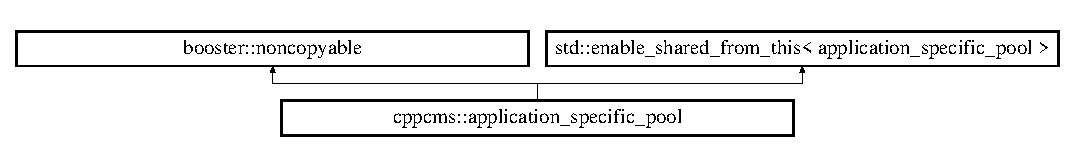
\includegraphics[height=1.595442cm]{classcppcms_1_1application__specific__pool}
\end{center}
\end{figure}
\subsection*{Public Member Functions}
\begin{DoxyCompactItemize}
\item 
{\bf booster\+::intrusive\+\_\+ptr}$<$ {\bf application} $>$ {\bf asynchronous\+\_\+application\+\_\+by\+\_\+io\+\_\+service} ({\bf booster\+::aio\+::io\+\_\+service} \&io\+\_\+srv, {\bf cppcms\+::service} \&srv)
\item 
{\bf booster\+::intrusive\+\_\+ptr}$<$ {\bf application} $>$ {\bf asynchronous\+\_\+application\+\_\+by\+\_\+io\+\_\+service} ({\bf booster\+::aio\+::io\+\_\+service} \&io\+\_\+srv)
\end{DoxyCompactItemize}
\subsection*{Protected Member Functions}
\begin{DoxyCompactItemize}
\item 
virtual {\bf application} $\ast$ {\bf new\+\_\+application} ({\bf service} \&srv)=0
\end{DoxyCompactItemize}
\subsection*{Friends}
\begin{DoxyCompactItemize}
\item 
class {\bfseries applications\+\_\+pool}\label{classcppcms_1_1application__specific__pool_a30f874a0e0276d427a1e284dc94255fc}

\item 
class {\bfseries application}\label{classcppcms_1_1application__specific__pool_a5b97104505447c42689b96b15027d832}

\item 
class {\bfseries http\+::context}\label{classcppcms_1_1application__specific__pool_a9b7b48313dd25fddf8cea424f99697e5}

\item 
void {\bfseries booster\+::intrusive\+\_\+ptr\+\_\+release} ({\bf cppcms\+::application} $\ast$app)\label{classcppcms_1_1application__specific__pool_ade262871b4f39bdcafba817c4486f499}

\end{DoxyCompactItemize}


\subsection{Detailed Description}
an interface for creating user applications 

\doxyref{New in Cpp\+C\+MS 1.\+2}{p.}{v1_2} 

\subsection{Member Function Documentation}
\index{cppcms\+::application\+\_\+specific\+\_\+pool@{cppcms\+::application\+\_\+specific\+\_\+pool}!asynchronous\+\_\+application\+\_\+by\+\_\+io\+\_\+service@{asynchronous\+\_\+application\+\_\+by\+\_\+io\+\_\+service}}
\index{asynchronous\+\_\+application\+\_\+by\+\_\+io\+\_\+service@{asynchronous\+\_\+application\+\_\+by\+\_\+io\+\_\+service}!cppcms\+::application\+\_\+specific\+\_\+pool@{cppcms\+::application\+\_\+specific\+\_\+pool}}
\subsubsection[{asynchronous\+\_\+application\+\_\+by\+\_\+io\+\_\+service(booster\+::aio\+::io\+\_\+service \&io\+\_\+srv, cppcms\+::service \&srv)}]{\setlength{\rightskip}{0pt plus 5cm}{\bf booster\+::intrusive\+\_\+ptr}$<${\bf application}$>$ cppcms\+::application\+\_\+specific\+\_\+pool\+::asynchronous\+\_\+application\+\_\+by\+\_\+io\+\_\+service (
\begin{DoxyParamCaption}
\item[{{\bf booster\+::aio\+::io\+\_\+service} \&}]{io\+\_\+srv, }
\item[{{\bf cppcms\+::service} \&}]{srv}
\end{DoxyParamCaption}
)}\label{classcppcms_1_1application__specific__pool_a503dad62f37f950e015f5b3cf69b9136}
Returns asynchronous application that runs at given \doxyref{booster\+::aio\+::io\+\_\+service}{p.}{classbooster_1_1aio_1_1io__service} constext, it the application does not exist yet, it is created

Notes\+:


\begin{DoxyItemize}
\item if the application is created upon function call it would be created in the calling thread regardless if it is event loop thread or not
\item If the pool isn\textquotesingle{}t mounted as asynchronous pool then \doxyref{cppcms\+\_\+error}{p.}{classcppcms_1_1cppcms__error} is thrown
\item if the io\+\_\+srv isn\textquotesingle{}t main cppcms io\+\_\+service \doxyref{cppcms\+\_\+error}{p.}{classcppcms_1_1cppcms__error} is thrown 
\end{DoxyItemize}\index{cppcms\+::application\+\_\+specific\+\_\+pool@{cppcms\+::application\+\_\+specific\+\_\+pool}!asynchronous\+\_\+application\+\_\+by\+\_\+io\+\_\+service@{asynchronous\+\_\+application\+\_\+by\+\_\+io\+\_\+service}}
\index{asynchronous\+\_\+application\+\_\+by\+\_\+io\+\_\+service@{asynchronous\+\_\+application\+\_\+by\+\_\+io\+\_\+service}!cppcms\+::application\+\_\+specific\+\_\+pool@{cppcms\+::application\+\_\+specific\+\_\+pool}}
\subsubsection[{asynchronous\+\_\+application\+\_\+by\+\_\+io\+\_\+service(booster\+::aio\+::io\+\_\+service \&io\+\_\+srv)}]{\setlength{\rightskip}{0pt plus 5cm}{\bf booster\+::intrusive\+\_\+ptr}$<${\bf application}$>$ cppcms\+::application\+\_\+specific\+\_\+pool\+::asynchronous\+\_\+application\+\_\+by\+\_\+io\+\_\+service (
\begin{DoxyParamCaption}
\item[{{\bf booster\+::aio\+::io\+\_\+service} \&}]{io\+\_\+srv}
\end{DoxyParamCaption}
)}\label{classcppcms_1_1application__specific__pool_a8f819438f764bd0ff7fdaa6668816c8a}
Returns asynchronous application that runs at given \doxyref{booster\+::aio\+::io\+\_\+service}{p.}{classbooster_1_1aio_1_1io__service} constext, it the application does not exist yet N\+U\+LL pointer is returned

Notes\+:


\begin{DoxyItemize}
\item If the pool isn\textquotesingle{}t mounted as asynchronous pool then \doxyref{cppcms\+\_\+error}{p.}{classcppcms_1_1cppcms__error} is thrown
\item if the io\+\_\+srv isn\textquotesingle{}t main cppcms io\+\_\+service \doxyref{cppcms\+\_\+error}{p.}{classcppcms_1_1cppcms__error} is thrown 
\end{DoxyItemize}\index{cppcms\+::application\+\_\+specific\+\_\+pool@{cppcms\+::application\+\_\+specific\+\_\+pool}!new\+\_\+application@{new\+\_\+application}}
\index{new\+\_\+application@{new\+\_\+application}!cppcms\+::application\+\_\+specific\+\_\+pool@{cppcms\+::application\+\_\+specific\+\_\+pool}}
\subsubsection[{new\+\_\+application(service \&srv)=0}]{\setlength{\rightskip}{0pt plus 5cm}virtual {\bf application}$\ast$ cppcms\+::application\+\_\+specific\+\_\+pool\+::new\+\_\+application (
\begin{DoxyParamCaption}
\item[{{\bf service} \&}]{srv}
\end{DoxyParamCaption}
)\hspace{0.3cm}{\ttfamily [protected]}, {\ttfamily [pure virtual]}}\label{classcppcms_1_1application__specific__pool_af8acef67b879aad12c8a163b28c182b9}
Returns newly created instance of an application, its ownership is transferred 

The documentation for this class was generated from the following file\+:\begin{DoxyCompactItemize}
\item 
cppcms/applications\+\_\+pool.\+h\end{DoxyCompactItemize}

\section{cppcms\+:\+:applications\+\_\+pool Class Reference}
\label{classcppcms_1_1applications__pool}\index{cppcms\+::applications\+\_\+pool@{cppcms\+::applications\+\_\+pool}}


Application pool is the central class that holds user created applications.  




{\ttfamily \#include $<$cppcms/applications\+\_\+pool.\+h$>$}

\subsection*{Classes}
\begin{DoxyCompactItemize}
\item 
struct {\bf factory}
\begin{DoxyCompactList}\small\item\em a base class for user application factories -\/ to be deprecated, use \doxyref{application\+\_\+specific\+\_\+pool}{p.}{classcppcms_1_1application__specific__pool} instead \end{DoxyCompactList}\end{DoxyCompactItemize}
\subsection*{Public Member Functions}
\begin{DoxyCompactItemize}
\item 
void {\bf mount} (std\+::unique\+\_\+ptr$<$ {\bf factory} $>$ aps)
\item 
void {\bf mount} (std\+::unique\+\_\+ptr$<$ {\bf factory} $>$ aps, {\bf mount\+\_\+point} const \&point)
\item 
void {\bf mount} ({\bf booster\+::intrusive\+\_\+ptr}$<$ {\bf application} $>$ app)
\item 
void {\bf mount} ({\bf booster\+::intrusive\+\_\+ptr}$<$ {\bf application} $>$ app, {\bf mount\+\_\+point} const \&point)
\item 
void {\bf mount} (booster\+::shared\+\_\+ptr$<$ {\bf application\+\_\+specific\+\_\+pool} $>$ gen, int application\+\_\+options=0)
\item 
void {\bf mount} (booster\+::shared\+\_\+ptr$<$ {\bf application\+\_\+specific\+\_\+pool} $>$ gen, {\bf mount\+\_\+point} const \&point, int application\+\_\+options=0)
\item 
void {\bf unmount} (booster\+::weak\+\_\+ptr$<$ {\bf application\+\_\+specific\+\_\+pool} $>$ gen)
\end{DoxyCompactItemize}


\subsection{Detailed Description}
Application pool is the central class that holds user created applications. 

Form the user perspective this class provides an A\+PI for mounting user application to the Cpp\+C\+MS service.

There are two kind of {\itshape mount} member functions, that allow\+:


\begin{DoxyItemize}
\item Mounting a {\itshape factory} of user applications -- for execution of synchronous requests by multiple instances of application.
\item Mounting single application -- for processing asynchronous requests by single instance of an application
\end{DoxyItemize}

The life cycle of synchronous application is defined by application pool itself, and the life cycle of asynchronous depends on its own reference count.

This class is thread safe and can be accessed from multiple threads simultaneously. 

\subsection{Member Function Documentation}
\index{cppcms\+::applications\+\_\+pool@{cppcms\+::applications\+\_\+pool}!mount@{mount}}
\index{mount@{mount}!cppcms\+::applications\+\_\+pool@{cppcms\+::applications\+\_\+pool}}
\subsubsection[{mount(std\+::unique\+\_\+ptr$<$ factory $>$ aps)}]{\setlength{\rightskip}{0pt plus 5cm}void cppcms\+::applications\+\_\+pool\+::mount (
\begin{DoxyParamCaption}
\item[{std\+::unique\+\_\+ptr$<$ {\bf factory} $>$}]{aps}
\end{DoxyParamCaption}
)}\label{classcppcms_1_1applications__pool_a0ba4c771958316a29da12403544e3f37}
Mount an application factory {\itshape aps} for processing of any incoming requests. Application would receive P\+A\+T\+H\+\_\+\+I\+N\+FO C\+GI variable for U\+RL matching.

This member function is thread safe.

\begin{DoxyRefDesc}{Deprecated}
\item[{\bf Deprecated}]Use \doxyref{mount(booster\+::shared\+\_\+ptr$<$application\+\_\+specific\+\_\+pool$>$ gen,int application\+\_\+options)}{p.}{classcppcms_1_1applications__pool_a00db03788459250a105a63e1cfde7d8a} instead \end{DoxyRefDesc}
\index{cppcms\+::applications\+\_\+pool@{cppcms\+::applications\+\_\+pool}!mount@{mount}}
\index{mount@{mount}!cppcms\+::applications\+\_\+pool@{cppcms\+::applications\+\_\+pool}}
\subsubsection[{mount(std\+::unique\+\_\+ptr$<$ factory $>$ aps, mount\+\_\+point const \&point)}]{\setlength{\rightskip}{0pt plus 5cm}void cppcms\+::applications\+\_\+pool\+::mount (
\begin{DoxyParamCaption}
\item[{std\+::unique\+\_\+ptr$<$ {\bf factory} $>$}]{aps, }
\item[{{\bf mount\+\_\+point} const \&}]{point}
\end{DoxyParamCaption}
)}\label{classcppcms_1_1applications__pool_a7639d6776b5357d96d030c0981f8c578}
Mount an application factory {\itshape app} by \doxyref{mount\+\_\+point}{p.}{classcppcms_1_1mount__point} {\itshape point} application matching and U\+RL selection rules

This member function is thread safe.

\begin{DoxyRefDesc}{Deprecated}
\item[{\bf Deprecated}]Use \doxyref{mount(booster\+::shared\+\_\+ptr$<$application\+\_\+specific\+\_\+pool$>$ gen,mount\+\_\+point const \&point,int application\+\_\+options)}{p.}{classcppcms_1_1applications__pool_aee865cfed576d1b3ddc0eb190ba12ab9} instead \end{DoxyRefDesc}
\index{cppcms\+::applications\+\_\+pool@{cppcms\+::applications\+\_\+pool}!mount@{mount}}
\index{mount@{mount}!cppcms\+::applications\+\_\+pool@{cppcms\+::applications\+\_\+pool}}
\subsubsection[{mount(booster\+::intrusive\+\_\+ptr$<$ application $>$ app)}]{\setlength{\rightskip}{0pt plus 5cm}void cppcms\+::applications\+\_\+pool\+::mount (
\begin{DoxyParamCaption}
\item[{{\bf booster\+::intrusive\+\_\+ptr}$<$ {\bf application} $>$}]{app}
\end{DoxyParamCaption}
)}\label{classcppcms_1_1applications__pool_a5df195e454c857c4c064f8593c76fc45}
Mount an asynchronous application {\itshape app} for processing of any incoming requests. Application would receive P\+A\+T\+H\+\_\+\+I\+N\+FO C\+GI variable for U\+RL matching.

This member function is thread safe.

\begin{DoxyRefDesc}{Deprecated}
\item[{\bf Deprecated}]Use \doxyref{mount(booster\+::shared\+\_\+ptr$<$application\+\_\+specific\+\_\+pool$>$ gen,int application\+\_\+options)}{p.}{classcppcms_1_1applications__pool_a00db03788459250a105a63e1cfde7d8a} with application\+\_\+options=\doxyref{app\+::asynchronous}{p.}{namespacecppcms_1_1app_a6e1f18add53bf1b4e590de8c9fee3dcd} instead \end{DoxyRefDesc}
\index{cppcms\+::applications\+\_\+pool@{cppcms\+::applications\+\_\+pool}!mount@{mount}}
\index{mount@{mount}!cppcms\+::applications\+\_\+pool@{cppcms\+::applications\+\_\+pool}}
\subsubsection[{mount(booster\+::intrusive\+\_\+ptr$<$ application $>$ app, mount\+\_\+point const \&point)}]{\setlength{\rightskip}{0pt plus 5cm}void cppcms\+::applications\+\_\+pool\+::mount (
\begin{DoxyParamCaption}
\item[{{\bf booster\+::intrusive\+\_\+ptr}$<$ {\bf application} $>$}]{app, }
\item[{{\bf mount\+\_\+point} const \&}]{point}
\end{DoxyParamCaption}
)}\label{classcppcms_1_1applications__pool_a3fefe91fd5a4012ae0cf66aecc0bcbc4}
Mount an asynchronous application {\itshape app} by \doxyref{mount\+\_\+point}{p.}{classcppcms_1_1mount__point} {\itshape point} application matching and U\+RL selection rules

This member function is thread safe.

\begin{DoxyRefDesc}{Deprecated}
\item[{\bf Deprecated}]Use \doxyref{mount(booster\+::shared\+\_\+ptr$<$application\+\_\+specific\+\_\+pool$>$ gen,mount\+\_\+point const \&point,int application\+\_\+options)}{p.}{classcppcms_1_1applications__pool_aee865cfed576d1b3ddc0eb190ba12ab9} with application\+\_\+options=\doxyref{app\+::asynchronous}{p.}{namespacecppcms_1_1app_a6e1f18add53bf1b4e590de8c9fee3dcd} instead \end{DoxyRefDesc}
\index{cppcms\+::applications\+\_\+pool@{cppcms\+::applications\+\_\+pool}!mount@{mount}}
\index{mount@{mount}!cppcms\+::applications\+\_\+pool@{cppcms\+::applications\+\_\+pool}}
\subsubsection[{mount(booster\+::shared\+\_\+ptr$<$ application\+\_\+specific\+\_\+pool $>$ gen, int application\+\_\+options=0)}]{\setlength{\rightskip}{0pt plus 5cm}void cppcms\+::applications\+\_\+pool\+::mount (
\begin{DoxyParamCaption}
\item[{booster\+::shared\+\_\+ptr$<$ {\bf application\+\_\+specific\+\_\+pool} $>$}]{gen, }
\item[{int}]{application\+\_\+options = {\ttfamily 0}}
\end{DoxyParamCaption}
)}\label{classcppcms_1_1applications__pool_a00db03788459250a105a63e1cfde7d8a}
Mount a \doxyref{application\+\_\+specific\+\_\+pool}{p.}{classcppcms_1_1application__specific__pool} for an application that processes all requests, path provided to application\textquotesingle{}s main is P\+A\+T\+H\+\_\+\+I\+N\+FO

{\itshape application\+\_\+options} allow to specify mode of operation -\/ synchronous, asynchronous, see namespace \doxyref{cppcms\+::app}{p.}{namespacecppcms_1_1app}

Note\+: \doxyref{applications\+\_\+pool}{p.}{classcppcms_1_1applications__pool} owns gen now and is responsible for destroying it

This member function is thread safe.

\doxyref{New in Cpp\+C\+MS 1.\+2}{p.}{v1_2} \index{cppcms\+::applications\+\_\+pool@{cppcms\+::applications\+\_\+pool}!mount@{mount}}
\index{mount@{mount}!cppcms\+::applications\+\_\+pool@{cppcms\+::applications\+\_\+pool}}
\subsubsection[{mount(booster\+::shared\+\_\+ptr$<$ application\+\_\+specific\+\_\+pool $>$ gen, mount\+\_\+point const \&point, int application\+\_\+options=0)}]{\setlength{\rightskip}{0pt plus 5cm}void cppcms\+::applications\+\_\+pool\+::mount (
\begin{DoxyParamCaption}
\item[{booster\+::shared\+\_\+ptr$<$ {\bf application\+\_\+specific\+\_\+pool} $>$}]{gen, }
\item[{{\bf mount\+\_\+point} const \&}]{point, }
\item[{int}]{application\+\_\+options = {\ttfamily 0}}
\end{DoxyParamCaption}
)}\label{classcppcms_1_1applications__pool_aee865cfed576d1b3ddc0eb190ba12ab9}
Mount a \doxyref{application\+\_\+specific\+\_\+pool}{p.}{classcppcms_1_1application__specific__pool} to a specific mount point

{\itshape application\+\_\+options} allow to specify mode of operation -\/ synchronous, asynchronous, see namespace \doxyref{cppcms\+::app}{p.}{namespacecppcms_1_1app}

Note\+: \doxyref{applications\+\_\+pool}{p.}{classcppcms_1_1applications__pool} owns gen now and is responsible for destroying it

This member function is thread safe.

\doxyref{New in Cpp\+C\+MS 1.\+2}{p.}{v1_2} \index{cppcms\+::applications\+\_\+pool@{cppcms\+::applications\+\_\+pool}!unmount@{unmount}}
\index{unmount@{unmount}!cppcms\+::applications\+\_\+pool@{cppcms\+::applications\+\_\+pool}}
\subsubsection[{unmount(booster\+::weak\+\_\+ptr$<$ application\+\_\+specific\+\_\+pool $>$ gen)}]{\setlength{\rightskip}{0pt plus 5cm}void cppcms\+::applications\+\_\+pool\+::unmount (
\begin{DoxyParamCaption}
\item[{booster\+::weak\+\_\+ptr$<$ {\bf application\+\_\+specific\+\_\+pool} $>$}]{gen}
\end{DoxyParamCaption}
)}\label{classcppcms_1_1applications__pool_a315961ad0c7d9ddb620b395802b6c291}
Unmount an \doxyref{application\+\_\+specific\+\_\+pool}{p.}{classcppcms_1_1application__specific__pool} from the general pool.

Notes\+:


\begin{DoxyItemize}
\item Exiting request would continue to be executed
\item There is no guarantee when and in which thread application objects would be destroyed upon use of unmount
\item applications in the pool using thread\+\_\+specific policy would be destroyed only on thread exit (i.\+e. when threads of thread pool are destroyed)
\end{DoxyItemize}

This member function is thread safe.

\doxyref{New in Cpp\+C\+MS 1.\+2}{p.}{v1_2} 

The documentation for this class was generated from the following file\+:\begin{DoxyCompactItemize}
\item 
cppcms/applications\+\_\+pool.\+h\end{DoxyCompactItemize}

\section{cppcms\+:\+:archive Class Reference}
\label{classcppcms_1_1archive}\index{cppcms\+::archive@{cppcms\+::archive}}


Class that represents a binary archive that can be stored in persistent storage or transfered.  




{\ttfamily \#include $<$cppcms/serialization\+\_\+classes.\+h$>$}

\subsection*{Public Types}
\begin{DoxyCompactItemize}
\item 
enum {\bf mode\+\_\+type} \{ {\bfseries save\+\_\+to\+\_\+archive}, 
{\bfseries load\+\_\+from\+\_\+archive}
 \}
\end{DoxyCompactItemize}
\subsection*{Public Member Functions}
\begin{DoxyCompactItemize}
\item 
void {\bf reserve} (size\+\_\+t size)
\item 
void {\bf write\+\_\+chunk} (void const $\ast$begin, size\+\_\+t len)
\item 
void {\bf read\+\_\+chunk} (void $\ast$begin, size\+\_\+t len)
\item 
size\+\_\+t {\bf next\+\_\+chunk\+\_\+size} ()
\item 
bool {\bf eof} ()
\item 
std\+::string {\bf read\+\_\+chunk\+\_\+as\+\_\+string} ()
\item 
void {\bf mode} ({\bf mode\+\_\+type} m)
\item 
{\bf mode\+\_\+type} {\bf mode} ()
\item 
void {\bf reset} ()
\item 
std\+::string {\bf str} ()
\item 
void {\bf str} (std\+::string const \&str)
\item 
{\bf archive} ()
\item 
{\bf $\sim$archive} ()
\item 
{\bf archive} ({\bf archive} const \&)
\item 
{\bf archive} const \& {\bf operator=} ({\bf archive} const \&)
\item 
{\bf archive} ({\bf archive} \&\&)
\item 
{\bf archive} \& {\bf operator=} ({\bf archive} \&\&)
\end{DoxyCompactItemize}


\subsection{Detailed Description}
Class that represents a binary archive that can be stored in persistent storage or transfered. 

\subsection{Member Enumeration Documentation}
\index{cppcms\+::archive@{cppcms\+::archive}!mode\+\_\+type@{mode\+\_\+type}}
\index{mode\+\_\+type@{mode\+\_\+type}!cppcms\+::archive@{cppcms\+::archive}}
\subsubsection[{mode\+\_\+type}]{\setlength{\rightskip}{0pt plus 5cm}enum {\bf cppcms\+::archive\+::mode\+\_\+type}}\label{classcppcms_1_1archive_a46fa7dca190eadf25c66ccd50d090fa5}
Operations mode on archive 

\subsection{Constructor \& Destructor Documentation}
\index{cppcms\+::archive@{cppcms\+::archive}!archive@{archive}}
\index{archive@{archive}!cppcms\+::archive@{cppcms\+::archive}}
\subsubsection[{archive()}]{\setlength{\rightskip}{0pt plus 5cm}cppcms\+::archive\+::archive (
\begin{DoxyParamCaption}
{}
\end{DoxyParamCaption}
)}\label{classcppcms_1_1archive_ace4d87706d13845807f76cb53da36c89}
Create new archive, by default in save\+\_\+to\+\_\+archive mode \index{cppcms\+::archive@{cppcms\+::archive}!````~archive@{$\sim$archive}}
\index{````~archive@{$\sim$archive}!cppcms\+::archive@{cppcms\+::archive}}
\subsubsection[{$\sim$archive()}]{\setlength{\rightskip}{0pt plus 5cm}cppcms\+::archive\+::$\sim$archive (
\begin{DoxyParamCaption}
{}
\end{DoxyParamCaption}
)}\label{classcppcms_1_1archive_a9be4ac7e156e78f07bc30512f9228b37}
Destructor \index{cppcms\+::archive@{cppcms\+::archive}!archive@{archive}}
\index{archive@{archive}!cppcms\+::archive@{cppcms\+::archive}}
\subsubsection[{archive(archive const \&)}]{\setlength{\rightskip}{0pt plus 5cm}cppcms\+::archive\+::archive (
\begin{DoxyParamCaption}
\item[{{\bf archive} const \&}]{}
\end{DoxyParamCaption}
)}\label{classcppcms_1_1archive_ab2cfb65276577d4a984276fe1476af3b}
Copy archive (avoid it) \index{cppcms\+::archive@{cppcms\+::archive}!archive@{archive}}
\index{archive@{archive}!cppcms\+::archive@{cppcms\+::archive}}
\subsubsection[{archive(archive \&\&)}]{\setlength{\rightskip}{0pt plus 5cm}cppcms\+::archive\+::archive (
\begin{DoxyParamCaption}
\item[{{\bf archive} \&\&}]{}
\end{DoxyParamCaption}
)}\label{classcppcms_1_1archive_a70630e83055d1c94528fc5da8a9d159e}
Move ctor archive 

\subsection{Member Function Documentation}
\index{cppcms\+::archive@{cppcms\+::archive}!eof@{eof}}
\index{eof@{eof}!cppcms\+::archive@{cppcms\+::archive}}
\subsubsection[{eof()}]{\setlength{\rightskip}{0pt plus 5cm}bool cppcms\+::archive\+::eof (
\begin{DoxyParamCaption}
{}
\end{DoxyParamCaption}
)}\label{classcppcms_1_1archive_a51b8f12712932526d15b7679b7be60f5}
Get if we got to the end of archive while reading \index{cppcms\+::archive@{cppcms\+::archive}!mode@{mode}}
\index{mode@{mode}!cppcms\+::archive@{cppcms\+::archive}}
\subsubsection[{mode(mode\+\_\+type m)}]{\setlength{\rightskip}{0pt plus 5cm}void cppcms\+::archive\+::mode (
\begin{DoxyParamCaption}
\item[{{\bf mode\+\_\+type}}]{m}
\end{DoxyParamCaption}
)}\label{classcppcms_1_1archive_a21d11b76aabfcd5702cae34031eeb890}
Set IO mode, resets pointer 

Referenced by cppcms\+::operator\&().

\index{cppcms\+::archive@{cppcms\+::archive}!mode@{mode}}
\index{mode@{mode}!cppcms\+::archive@{cppcms\+::archive}}
\subsubsection[{mode()}]{\setlength{\rightskip}{0pt plus 5cm}{\bf mode\+\_\+type} cppcms\+::archive\+::mode (
\begin{DoxyParamCaption}
{}
\end{DoxyParamCaption}
)}\label{classcppcms_1_1archive_a3d50427180c0ed663f1c833bcf31b78e}
Get IO mode \index{cppcms\+::archive@{cppcms\+::archive}!next\+\_\+chunk\+\_\+size@{next\+\_\+chunk\+\_\+size}}
\index{next\+\_\+chunk\+\_\+size@{next\+\_\+chunk\+\_\+size}!cppcms\+::archive@{cppcms\+::archive}}
\subsubsection[{next\+\_\+chunk\+\_\+size()}]{\setlength{\rightskip}{0pt plus 5cm}size\+\_\+t cppcms\+::archive\+::next\+\_\+chunk\+\_\+size (
\begin{DoxyParamCaption}
{}
\end{DoxyParamCaption}
)}\label{classcppcms_1_1archive_a5a146e203a30a644af14b2edf651ceca}
Get the size of the next chunk that can be read \index{cppcms\+::archive@{cppcms\+::archive}!operator=@{operator=}}
\index{operator=@{operator=}!cppcms\+::archive@{cppcms\+::archive}}
\subsubsection[{operator=(archive const \&)}]{\setlength{\rightskip}{0pt plus 5cm}{\bf archive} const\& cppcms\+::archive\+::operator= (
\begin{DoxyParamCaption}
\item[{{\bf archive} const \&}]{}
\end{DoxyParamCaption}
)}\label{classcppcms_1_1archive_a95dc7728b064e04a7ad77429b0b14c10}
Assign archive (avoid it) \index{cppcms\+::archive@{cppcms\+::archive}!operator=@{operator=}}
\index{operator=@{operator=}!cppcms\+::archive@{cppcms\+::archive}}
\subsubsection[{operator=(archive \&\&)}]{\setlength{\rightskip}{0pt plus 5cm}{\bf archive}\& cppcms\+::archive\+::operator= (
\begin{DoxyParamCaption}
\item[{{\bf archive} \&\&}]{}
\end{DoxyParamCaption}
)}\label{classcppcms_1_1archive_a46bcf7723286fb2cfefb81a47929f28b}
Move Assign archive \index{cppcms\+::archive@{cppcms\+::archive}!read\+\_\+chunk@{read\+\_\+chunk}}
\index{read\+\_\+chunk@{read\+\_\+chunk}!cppcms\+::archive@{cppcms\+::archive}}
\subsubsection[{read\+\_\+chunk(void $\ast$begin, size\+\_\+t len)}]{\setlength{\rightskip}{0pt plus 5cm}void cppcms\+::archive\+::read\+\_\+chunk (
\begin{DoxyParamCaption}
\item[{void $\ast$}]{begin, }
\item[{size\+\_\+t}]{len}
\end{DoxyParamCaption}
)}\label{classcppcms_1_1archive_a479f94fb64e07ee40ef0193c0ad0d877}
Read a chunk of size len from archive \index{cppcms\+::archive@{cppcms\+::archive}!read\+\_\+chunk\+\_\+as\+\_\+string@{read\+\_\+chunk\+\_\+as\+\_\+string}}
\index{read\+\_\+chunk\+\_\+as\+\_\+string@{read\+\_\+chunk\+\_\+as\+\_\+string}!cppcms\+::archive@{cppcms\+::archive}}
\subsubsection[{read\+\_\+chunk\+\_\+as\+\_\+string()}]{\setlength{\rightskip}{0pt plus 5cm}std\+::string cppcms\+::archive\+::read\+\_\+chunk\+\_\+as\+\_\+string (
\begin{DoxyParamCaption}
{}
\end{DoxyParamCaption}
)}\label{classcppcms_1_1archive_adb0aa39b5062fe8a02168660221f27e4}
Read next chunk as std\+::string \index{cppcms\+::archive@{cppcms\+::archive}!reserve@{reserve}}
\index{reserve@{reserve}!cppcms\+::archive@{cppcms\+::archive}}
\subsubsection[{reserve(size\+\_\+t size)}]{\setlength{\rightskip}{0pt plus 5cm}void cppcms\+::archive\+::reserve (
\begin{DoxyParamCaption}
\item[{size\+\_\+t}]{size}
\end{DoxyParamCaption}
)}\label{classcppcms_1_1archive_ace76201b57090ee058419329c40979dc}
Reserve some memory before we write actual data \index{cppcms\+::archive@{cppcms\+::archive}!reset@{reset}}
\index{reset@{reset}!cppcms\+::archive@{cppcms\+::archive}}
\subsubsection[{reset()}]{\setlength{\rightskip}{0pt plus 5cm}void cppcms\+::archive\+::reset (
\begin{DoxyParamCaption}
{}
\end{DoxyParamCaption}
)}\label{classcppcms_1_1archive_a2203d52ea2a3ef7092bc6251d8e0b5a1}
Reset IO pointer \index{cppcms\+::archive@{cppcms\+::archive}!str@{str}}
\index{str@{str}!cppcms\+::archive@{cppcms\+::archive}}
\subsubsection[{str()}]{\setlength{\rightskip}{0pt plus 5cm}std\+::string cppcms\+::archive\+::str (
\begin{DoxyParamCaption}
{}
\end{DoxyParamCaption}
)}\label{classcppcms_1_1archive_a4d1c05bf04123e91c7a96dd03f12daef}
Get serialized object memory \index{cppcms\+::archive@{cppcms\+::archive}!str@{str}}
\index{str@{str}!cppcms\+::archive@{cppcms\+::archive}}
\subsubsection[{str(std\+::string const \&str)}]{\setlength{\rightskip}{0pt plus 5cm}void cppcms\+::archive\+::str (
\begin{DoxyParamCaption}
\item[{std\+::string const \&}]{str}
\end{DoxyParamCaption}
)}\label{classcppcms_1_1archive_aab5bdd07069c4695827dcf5bdea3ed99}
Set serialized object memory, sets mode to load\+\_\+from\+\_\+archive \index{cppcms\+::archive@{cppcms\+::archive}!write\+\_\+chunk@{write\+\_\+chunk}}
\index{write\+\_\+chunk@{write\+\_\+chunk}!cppcms\+::archive@{cppcms\+::archive}}
\subsubsection[{write\+\_\+chunk(void const $\ast$begin, size\+\_\+t len)}]{\setlength{\rightskip}{0pt plus 5cm}void cppcms\+::archive\+::write\+\_\+chunk (
\begin{DoxyParamCaption}
\item[{void const $\ast$}]{begin, }
\item[{size\+\_\+t}]{len}
\end{DoxyParamCaption}
)}\label{classcppcms_1_1archive_ab4169104a497e4ec692cd4b2c420bc4d}
Write a chunk of size len to archive 

The documentation for this class was generated from the following file\+:\begin{DoxyCompactItemize}
\item 
cppcms/serialization\+\_\+classes.\+h\end{DoxyCompactItemize}

\section{cppcms\+:\+:archive\+\_\+error Class Reference}
\label{classcppcms_1_1archive__error}\index{cppcms\+::archive\+\_\+error@{cppcms\+::archive\+\_\+error}}


Error thrown in case of serialization error.  




{\ttfamily \#include $<$cppcms/serialization\+\_\+classes.\+h$>$}

Inheritance diagram for cppcms\+:\+:archive\+\_\+error\+:\begin{figure}[H]
\begin{center}
\leavevmode
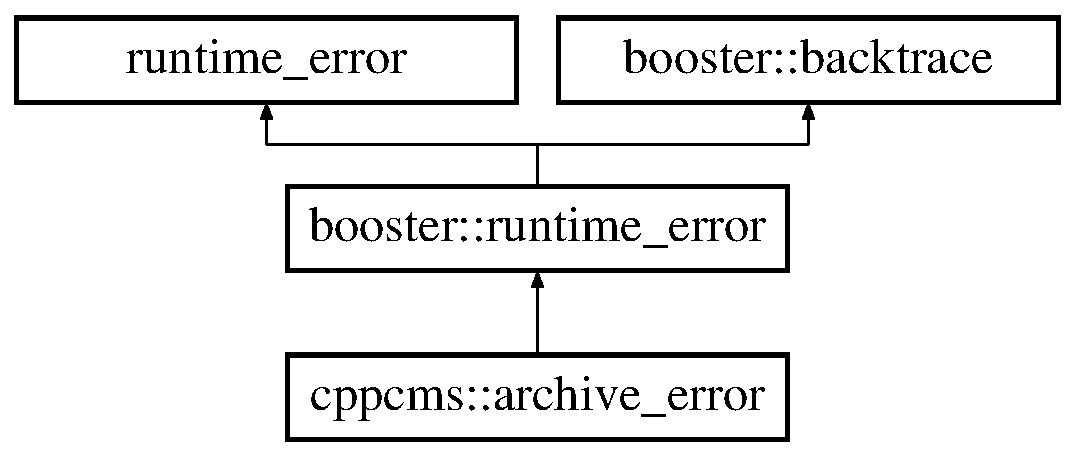
\includegraphics[height=3.000000cm]{classcppcms_1_1archive__error}
\end{center}
\end{figure}
\subsection*{Public Member Functions}
\begin{DoxyCompactItemize}
\item 
{\bfseries archive\+\_\+error} (std\+::string const \&e)\label{classcppcms_1_1archive__error_abe2df913b4c009ffb5fce90f0b81702e}

\end{DoxyCompactItemize}
\subsection*{Additional Inherited Members}


\subsection{Detailed Description}
Error thrown in case of serialization error. 

The documentation for this class was generated from the following file\+:\begin{DoxyCompactItemize}
\item 
cppcms/serialization\+\_\+classes.\+h\end{DoxyCompactItemize}

\section{cppcms\+:\+:archive\+\_\+traits$<$ Object $>$ Struct Template Reference}
\label{structcppcms_1_1archive__traits}\index{cppcms\+::archive\+\_\+traits$<$ Object $>$@{cppcms\+::archive\+\_\+traits$<$ Object $>$}}


Special traits class that describes how to serialize various objects that are not defived from \doxyref{serializable\+\_\+base}{p.}{classcppcms_1_1serializable__base}.  




{\ttfamily \#include $<$cppcms/serialization\+\_\+classes.\+h$>$}

\subsection*{Static Public Member Functions}
\begin{DoxyCompactItemize}
\item 
static void {\bf save} (Object const \&d, {\bf archive} \&a)
\item 
static void {\bf load} (Object \&d, {\bf archive} \&a)
\end{DoxyCompactItemize}


\subsection{Detailed Description}
\subsubsection*{template$<$typename Object$>$\\*
struct cppcms\+::archive\+\_\+traits$<$ Object $>$}

Special traits class that describes how to serialize various objects that are not defived from \doxyref{serializable\+\_\+base}{p.}{classcppcms_1_1serializable__base}. 

\subsection{Member Function Documentation}
\index{cppcms\+::archive\+\_\+traits@{cppcms\+::archive\+\_\+traits}!load@{load}}
\index{load@{load}!cppcms\+::archive\+\_\+traits@{cppcms\+::archive\+\_\+traits}}
\subsubsection[{load(\+Object \&d, archive \&a)}]{\setlength{\rightskip}{0pt plus 5cm}template$<$typename Object $>$ static void {\bf cppcms\+::archive\+\_\+traits}$<$ Object $>$\+::load (
\begin{DoxyParamCaption}
\item[{Object \&}]{d, }
\item[{{\bf archive} \&}]{a}
\end{DoxyParamCaption}
)\hspace{0.3cm}{\ttfamily [static]}}\label{structcppcms_1_1archive__traits_aa1f8400b5ae34ee663600c24635c0e4c}
Load object from archive function 

Referenced by cppcms\+::operator\&(), and cppcms\+::operator$>$$>$().

\index{cppcms\+::archive\+\_\+traits@{cppcms\+::archive\+\_\+traits}!save@{save}}
\index{save@{save}!cppcms\+::archive\+\_\+traits@{cppcms\+::archive\+\_\+traits}}
\subsubsection[{save(\+Object const \&d, archive \&a)}]{\setlength{\rightskip}{0pt plus 5cm}template$<$typename Object $>$ static void {\bf cppcms\+::archive\+\_\+traits}$<$ Object $>$\+::save (
\begin{DoxyParamCaption}
\item[{Object const \&}]{d, }
\item[{{\bf archive} \&}]{a}
\end{DoxyParamCaption}
)\hspace{0.3cm}{\ttfamily [static]}}\label{structcppcms_1_1archive__traits_ab880c09eeaf941991302fc33247b30e9}
Save object to archive function 

Referenced by cppcms\+::operator$<$$<$().



The documentation for this struct was generated from the following file\+:\begin{DoxyCompactItemize}
\item 
cppcms/serialization\+\_\+classes.\+h\end{DoxyCompactItemize}

\section{booster\+:\+:atomic\+\_\+counter Class Reference}
\label{classbooster_1_1atomic__counter}\index{booster\+::atomic\+\_\+counter@{booster\+::atomic\+\_\+counter}}


Atomic counter is a class that allows perform counting in thread safe way.  




{\ttfamily \#include $<$booster/booster/atomic\+\_\+counter.\+h$>$}

\subsection*{Public Member Functions}
\begin{DoxyCompactItemize}
\item 
{\bf atomic\+\_\+counter} (long v)
\item 
long {\bf operator++} ()
\item 
long {\bf operator-\/-\/} ()
\item 
{\bf operator long} () const 
\end{DoxyCompactItemize}


\subsection{Detailed Description}
Atomic counter is a class that allows perform counting in thread safe way. 

\subsection{Constructor \& Destructor Documentation}
\index{booster\+::atomic\+\_\+counter@{booster\+::atomic\+\_\+counter}!atomic\+\_\+counter@{atomic\+\_\+counter}}
\index{atomic\+\_\+counter@{atomic\+\_\+counter}!booster\+::atomic\+\_\+counter@{booster\+::atomic\+\_\+counter}}
\subsubsection[{atomic\+\_\+counter(long v)}]{\setlength{\rightskip}{0pt plus 5cm}booster\+::atomic\+\_\+counter\+::atomic\+\_\+counter (
\begin{DoxyParamCaption}
\item[{long}]{v}
\end{DoxyParamCaption}
)\hspace{0.3cm}{\ttfamily [explicit]}}\label{classbooster_1_1atomic__counter_aa196300e2e02b4b640135fcb878ca231}
Create a counter with initial value v 

\subsection{Member Function Documentation}
\index{booster\+::atomic\+\_\+counter@{booster\+::atomic\+\_\+counter}!operator long@{operator long}}
\index{operator long@{operator long}!booster\+::atomic\+\_\+counter@{booster\+::atomic\+\_\+counter}}
\subsubsection[{operator long() const }]{\setlength{\rightskip}{0pt plus 5cm}booster\+::atomic\+\_\+counter\+::operator long (
\begin{DoxyParamCaption}
{}
\end{DoxyParamCaption}
) const\hspace{0.3cm}{\ttfamily [inline]}}\label{classbooster_1_1atomic__counter_a30ee8319a82f03810766d74a7212c66a}
Return current value -\/ atomically \index{booster\+::atomic\+\_\+counter@{booster\+::atomic\+\_\+counter}!operator++@{operator++}}
\index{operator++@{operator++}!booster\+::atomic\+\_\+counter@{booster\+::atomic\+\_\+counter}}
\subsubsection[{operator++()}]{\setlength{\rightskip}{0pt plus 5cm}long booster\+::atomic\+\_\+counter\+::operator++ (
\begin{DoxyParamCaption}
{}
\end{DoxyParamCaption}
)\hspace{0.3cm}{\ttfamily [inline]}}\label{classbooster_1_1atomic__counter_a2084017688a3105cd45c50b615884a7c}
Increment and return the result after increment atomically \index{booster\+::atomic\+\_\+counter@{booster\+::atomic\+\_\+counter}!operator-\/-\/@{operator-\/-\/}}
\index{operator-\/-\/@{operator-\/-\/}!booster\+::atomic\+\_\+counter@{booster\+::atomic\+\_\+counter}}
\subsubsection[{operator-\/-\/()}]{\setlength{\rightskip}{0pt plus 5cm}long booster\+::atomic\+\_\+counter\+::operator-\/-\/ (
\begin{DoxyParamCaption}
{}
\end{DoxyParamCaption}
)\hspace{0.3cm}{\ttfamily [inline]}}\label{classbooster_1_1atomic__counter_afb02b5cb2b749a930d5fac39a2412262}
Decrement and return the result after decrement atomically 

The documentation for this class was generated from the following file\+:\begin{DoxyCompactItemize}
\item 
booster/atomic\+\_\+counter.\+h\end{DoxyCompactItemize}

\section{booster\+:\+:backtrace Class Reference}
\label{classbooster_1_1backtrace}\index{booster\+::backtrace@{booster\+::backtrace}}


the class that records the stack trace when it is created,  




{\ttfamily \#include $<$booster/booster/backtrace.\+h$>$}

Inheritance diagram for booster\+:\+:backtrace\+:\begin{figure}[H]
\begin{center}
\leavevmode
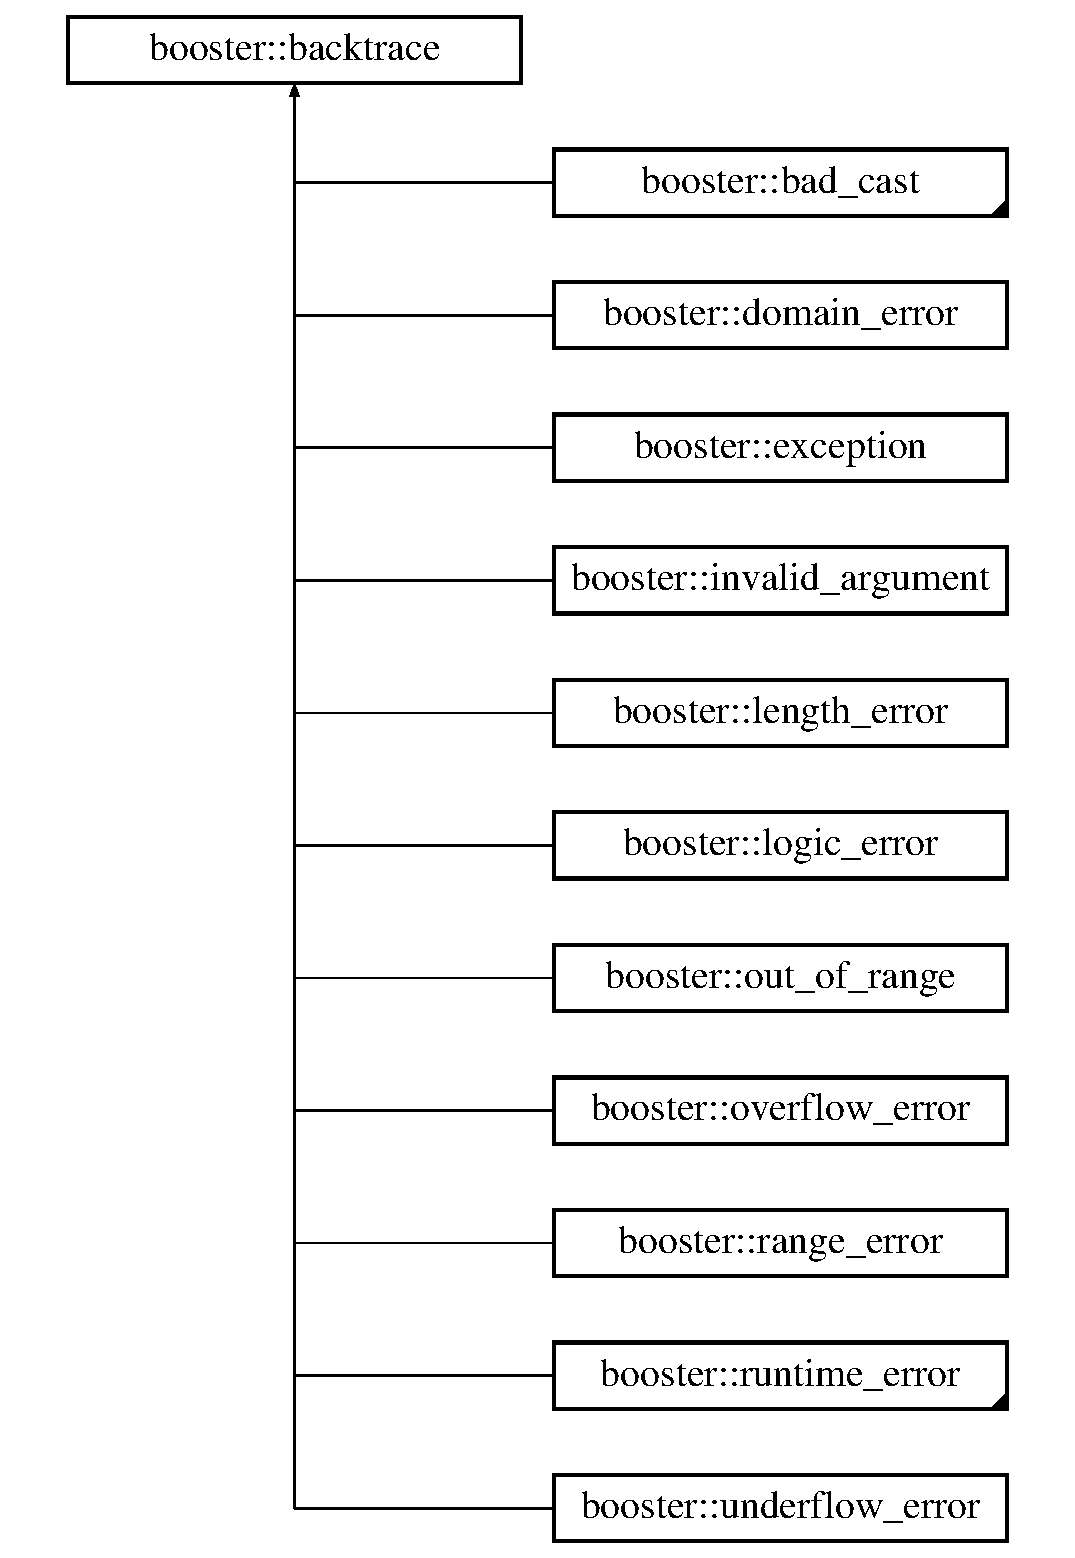
\includegraphics[height=12.000000cm]{classbooster_1_1backtrace}
\end{center}
\end{figure}
\subsection*{Public Member Functions}
\begin{DoxyCompactItemize}
\item 
{\bf backtrace} (size\+\_\+t frames\+\_\+no={\bf default\+\_\+stack\+\_\+size})
\item 
size\+\_\+t {\bf stack\+\_\+size} () const 
\item 
void $\ast$ {\bf return\+\_\+address} (unsigned frame\+\_\+no) const 
\item 
void {\bf trace\+\_\+line} (unsigned frame\+\_\+no, std\+::ostream \&out) const 
\item 
std\+::string {\bf trace\+\_\+line} (unsigned frame\+\_\+no) const 
\item 
std\+::string {\bf trace} () const 
\item 
void {\bf trace} (std\+::ostream \&out) const 
\end{DoxyCompactItemize}
\subsection*{Static Public Attributes}
\begin{DoxyCompactItemize}
\item 
static size\+\_\+t const {\bf default\+\_\+stack\+\_\+size} = 32
\end{DoxyCompactItemize}


\subsection{Detailed Description}
the class that records the stack trace when it is created, 

It is a base class for all exceptions that record stack trace 

\subsection{Constructor \& Destructor Documentation}
\index{booster\+::backtrace@{booster\+::backtrace}!backtrace@{backtrace}}
\index{backtrace@{backtrace}!booster\+::backtrace@{booster\+::backtrace}}
\subsubsection[{backtrace(size\+\_\+t frames\+\_\+no=default\+\_\+stack\+\_\+size)}]{\setlength{\rightskip}{0pt plus 5cm}booster\+::backtrace\+::backtrace (
\begin{DoxyParamCaption}
\item[{size\+\_\+t}]{frames\+\_\+no = {\ttfamily {\bf default\+\_\+stack\+\_\+size}}}
\end{DoxyParamCaption}
)\hspace{0.3cm}{\ttfamily [inline]}}\label{classbooster_1_1backtrace_ad7953e9c5fb97768afdc66f5fa448514}
Create stack trace recording at most {\itshape frames\+\_\+no} stack frames 

References booster\+::stack\+\_\+trace\+::trace().



\subsection{Member Function Documentation}
\index{booster\+::backtrace@{booster\+::backtrace}!return\+\_\+address@{return\+\_\+address}}
\index{return\+\_\+address@{return\+\_\+address}!booster\+::backtrace@{booster\+::backtrace}}
\subsubsection[{return\+\_\+address(unsigned frame\+\_\+no) const }]{\setlength{\rightskip}{0pt plus 5cm}void$\ast$ booster\+::backtrace\+::return\+\_\+address (
\begin{DoxyParamCaption}
\item[{unsigned}]{frame\+\_\+no}
\end{DoxyParamCaption}
) const\hspace{0.3cm}{\ttfamily [inline]}}\label{classbooster_1_1backtrace_a58e276d7fe9856a5e8d0999cb22e7d10}
Get the returned address for the stack frame number {\itshape frame\+\_\+no} \index{booster\+::backtrace@{booster\+::backtrace}!stack\+\_\+size@{stack\+\_\+size}}
\index{stack\+\_\+size@{stack\+\_\+size}!booster\+::backtrace@{booster\+::backtrace}}
\subsubsection[{stack\+\_\+size() const }]{\setlength{\rightskip}{0pt plus 5cm}size\+\_\+t booster\+::backtrace\+::stack\+\_\+size (
\begin{DoxyParamCaption}
{}
\end{DoxyParamCaption}
) const\hspace{0.3cm}{\ttfamily [inline]}}\label{classbooster_1_1backtrace_adb15203da5cb6e2f4c15d16ce703df4f}
Get the actual number of recorded stack frames \index{booster\+::backtrace@{booster\+::backtrace}!trace@{trace}}
\index{trace@{trace}!booster\+::backtrace@{booster\+::backtrace}}
\subsubsection[{trace() const }]{\setlength{\rightskip}{0pt plus 5cm}std\+::string booster\+::backtrace\+::trace (
\begin{DoxyParamCaption}
{}
\end{DoxyParamCaption}
) const\hspace{0.3cm}{\ttfamily [inline]}}\label{classbooster_1_1backtrace_ad50e49567d795065da36b4cf47b3e2f4}
Get full stack trace as a string 

References booster\+::stack\+\_\+trace\+::get\+\_\+symbols().

\index{booster\+::backtrace@{booster\+::backtrace}!trace@{trace}}
\index{trace@{trace}!booster\+::backtrace@{booster\+::backtrace}}
\subsubsection[{trace(std\+::ostream \&out) const }]{\setlength{\rightskip}{0pt plus 5cm}void booster\+::backtrace\+::trace (
\begin{DoxyParamCaption}
\item[{std\+::ostream \&}]{out}
\end{DoxyParamCaption}
) const\hspace{0.3cm}{\ttfamily [inline]}}\label{classbooster_1_1backtrace_a24ca881e26bd7396d827a7d0b755c4bf}
Print full stack trace to a stream {\itshape out} 

References booster\+::stack\+\_\+trace\+::write\+\_\+symbols().

\index{booster\+::backtrace@{booster\+::backtrace}!trace\+\_\+line@{trace\+\_\+line}}
\index{trace\+\_\+line@{trace\+\_\+line}!booster\+::backtrace@{booster\+::backtrace}}
\subsubsection[{trace\+\_\+line(unsigned frame\+\_\+no, std\+::ostream \&out) const }]{\setlength{\rightskip}{0pt plus 5cm}void booster\+::backtrace\+::trace\+\_\+line (
\begin{DoxyParamCaption}
\item[{unsigned}]{frame\+\_\+no, }
\item[{std\+::ostream \&}]{out}
\end{DoxyParamCaption}
) const\hspace{0.3cm}{\ttfamily [inline]}}\label{classbooster_1_1backtrace_a01b0ebc228110269a5a246ca13c1f77d}
Print the stack trace frame for the frame {\itshape frame\+\_\+no} to the stream {\itshape out} 

References booster\+::stack\+\_\+trace\+::write\+\_\+symbols().

\index{booster\+::backtrace@{booster\+::backtrace}!trace\+\_\+line@{trace\+\_\+line}}
\index{trace\+\_\+line@{trace\+\_\+line}!booster\+::backtrace@{booster\+::backtrace}}
\subsubsection[{trace\+\_\+line(unsigned frame\+\_\+no) const }]{\setlength{\rightskip}{0pt plus 5cm}std\+::string booster\+::backtrace\+::trace\+\_\+line (
\begin{DoxyParamCaption}
\item[{unsigned}]{frame\+\_\+no}
\end{DoxyParamCaption}
) const\hspace{0.3cm}{\ttfamily [inline]}}\label{classbooster_1_1backtrace_ae487b18c6a4c0ec875933e7ffca59578}
Get a readable stack trace frame for the frame {\itshape frame\+\_\+no} 

References booster\+::stack\+\_\+trace\+::get\+\_\+symbol().



\subsection{Member Data Documentation}
\index{booster\+::backtrace@{booster\+::backtrace}!default\+\_\+stack\+\_\+size@{default\+\_\+stack\+\_\+size}}
\index{default\+\_\+stack\+\_\+size@{default\+\_\+stack\+\_\+size}!booster\+::backtrace@{booster\+::backtrace}}
\subsubsection[{default\+\_\+stack\+\_\+size}]{\setlength{\rightskip}{0pt plus 5cm}size\+\_\+t const booster\+::backtrace\+::default\+\_\+stack\+\_\+size = 32\hspace{0.3cm}{\ttfamily [static]}}\label{classbooster_1_1backtrace_a0e1bcb70bc3845ca8cca8cf53782b048}
The default number of recorded frames 

The documentation for this class was generated from the following file\+:\begin{DoxyCompactItemize}
\item 
booster/backtrace.\+h\end{DoxyCompactItemize}

\section{booster\+:\+:bad\+\_\+callback\+\_\+call Class Reference}
\label{classbooster_1_1bad__callback__call}\index{booster\+::bad\+\_\+callback\+\_\+call@{booster\+::bad\+\_\+callback\+\_\+call}}


this exception is thrown in case of calling unassigned/empty function  




{\ttfamily \#include $<$booster/booster/callback.\+h$>$}

Inheritance diagram for booster\+:\+:bad\+\_\+callback\+\_\+call\+:\begin{figure}[H]
\begin{center}
\leavevmode
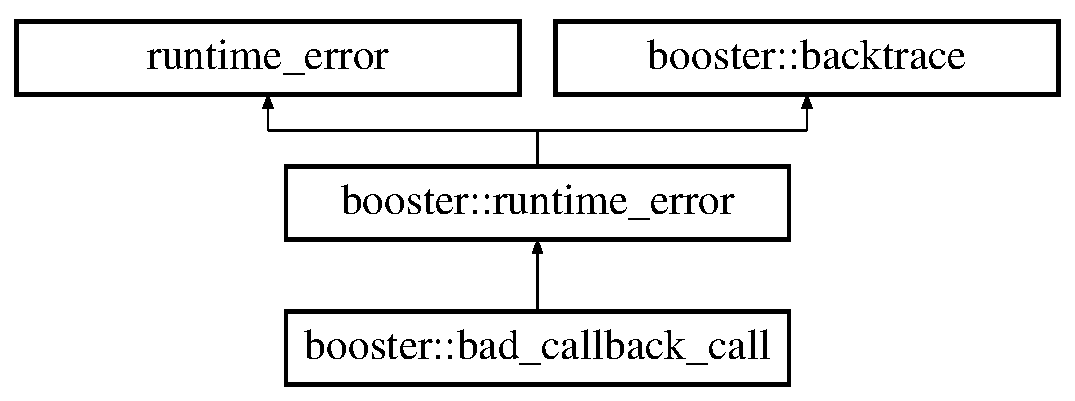
\includegraphics[height=3.000000cm]{classbooster_1_1bad__callback__call}
\end{center}
\end{figure}
\subsection*{Additional Inherited Members}


\subsection{Detailed Description}
this exception is thrown in case of calling unassigned/empty function 

The documentation for this class was generated from the following file\+:\begin{DoxyCompactItemize}
\item 
booster/callback.\+h\end{DoxyCompactItemize}

\section{booster\+:\+:bad\+\_\+cast Class Reference}
\label{classbooster_1_1bad__cast}\index{booster\+::bad\+\_\+cast@{booster\+::bad\+\_\+cast}}


Same as std\+::bad\+\_\+cast but records stack trace.  




{\ttfamily \#include $<$booster/booster/backtrace.\+h$>$}

Inheritance diagram for booster\+:\+:bad\+\_\+cast\+:\begin{figure}[H]
\begin{center}
\leavevmode
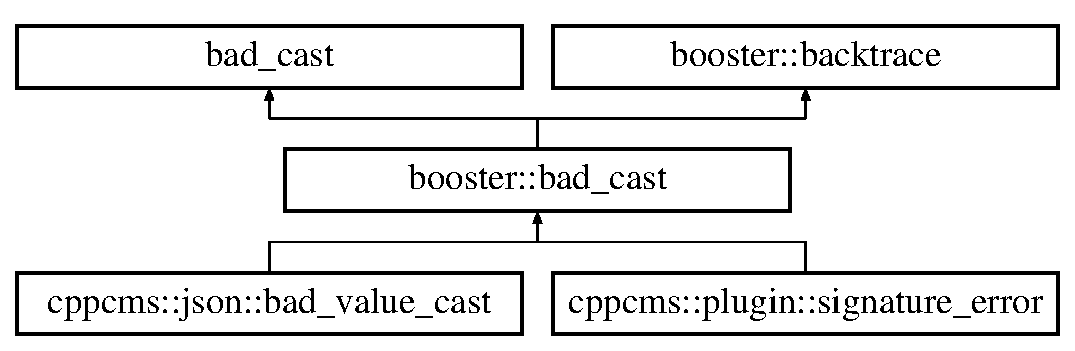
\includegraphics[height=3.000000cm]{classbooster_1_1bad__cast}
\end{center}
\end{figure}
\subsection*{Additional Inherited Members}


\subsection{Detailed Description}
Same as std\+::bad\+\_\+cast but records stack trace. 

The documentation for this class was generated from the following file\+:\begin{DoxyCompactItemize}
\item 
booster/backtrace.\+h\end{DoxyCompactItemize}

\section{booster\+:\+:nowide\+:\+:bad\+\_\+utf Class Reference}
\label{classbooster_1_1nowide_1_1bad__utf}\index{booster\+::nowide\+::bad\+\_\+utf@{booster\+::nowide\+::bad\+\_\+utf}}


This exception is thrown if invalid U\+T\+F-\/8 or U\+T\+F-\/16 is given as input.  




{\ttfamily \#include $<$booster/booster/nowide/convert.\+h$>$}

Inheritance diagram for booster\+:\+:nowide\+:\+:bad\+\_\+utf\+:\begin{figure}[H]
\begin{center}
\leavevmode
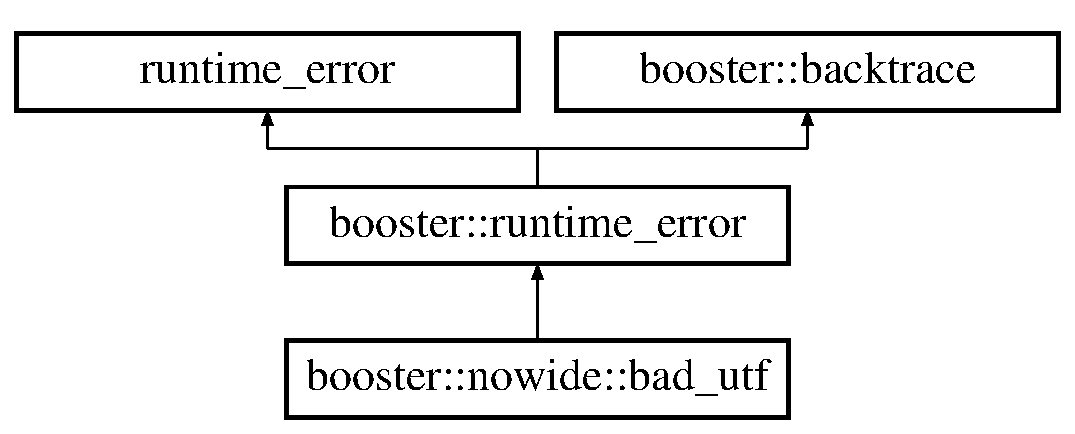
\includegraphics[height=3.000000cm]{classbooster_1_1nowide_1_1bad__utf}
\end{center}
\end{figure}
\subsection*{Additional Inherited Members}


\subsection{Detailed Description}
This exception is thrown if invalid U\+T\+F-\/8 or U\+T\+F-\/16 is given as input. 

The documentation for this class was generated from the following file\+:\begin{DoxyCompactItemize}
\item 
booster/nowide/convert.\+h\end{DoxyCompactItemize}

\section{cppcms\+:\+:json\+:\+:bad\+\_\+value\+\_\+cast Class Reference}
\label{classcppcms_1_1json_1_1bad__value__cast}\index{cppcms\+::json\+::bad\+\_\+value\+\_\+cast@{cppcms\+::json\+::bad\+\_\+value\+\_\+cast}}


The error that is thrown in case of bad conversion of \doxyref{json\+::value}{p.}{classcppcms_1_1json_1_1value} to ordinary value.  




{\ttfamily \#include $<$cppcms/json.\+h$>$}

Inheritance diagram for cppcms\+:\+:json\+:\+:bad\+\_\+value\+\_\+cast\+:\begin{figure}[H]
\begin{center}
\leavevmode
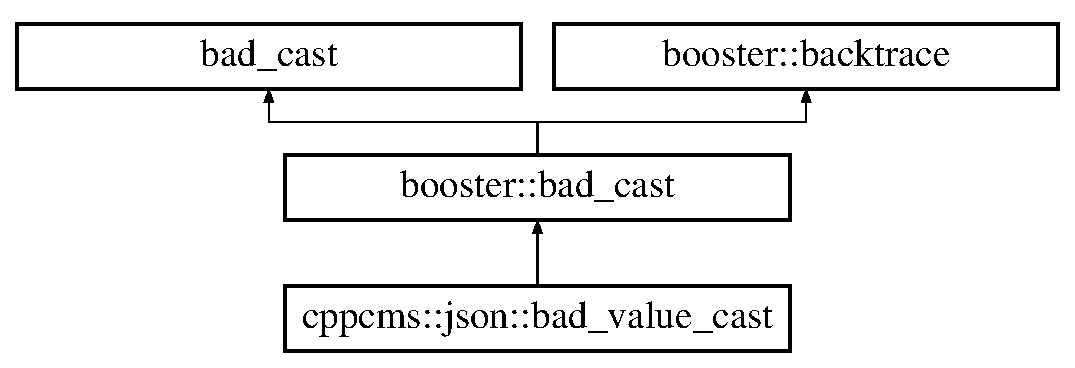
\includegraphics[height=3.000000cm]{classcppcms_1_1json_1_1bad__value__cast}
\end{center}
\end{figure}
\subsection*{Public Member Functions}
\begin{DoxyCompactItemize}
\item 
{\bfseries bad\+\_\+value\+\_\+cast} (std\+::string const \&s)\label{classcppcms_1_1json_1_1bad__value__cast_ae5488c2e9118120c77aed3d6a8d291db}

\item 
{\bfseries bad\+\_\+value\+\_\+cast} (std\+::string const \&s, {\bf json\+\_\+type} actual)\label{classcppcms_1_1json_1_1bad__value__cast_a48dfeac7fe8c77a1301389c56f02ccf0}

\item 
{\bfseries bad\+\_\+value\+\_\+cast} (std\+::string const \&s, {\bf json\+\_\+type} expected, {\bf json\+\_\+type} actual)\label{classcppcms_1_1json_1_1bad__value__cast_af7622585625529d0a74f711ac5eaee29}

\item 
virtual const char $\ast$ {\bfseries what} () const   throw ()\label{classcppcms_1_1json_1_1bad__value__cast_ae83a58ae4345791c01df6a9541547ee8}

\end{DoxyCompactItemize}
\subsection*{Additional Inherited Members}


\subsection{Detailed Description}
The error that is thrown in case of bad conversion of \doxyref{json\+::value}{p.}{classcppcms_1_1json_1_1value} to ordinary value. 

When implementing \doxyref{json\+::traits}{p.}{structcppcms_1_1json_1_1traits} for complex classes you are expected to throw this exception in case of invalid formatting 

The documentation for this class was generated from the following file\+:\begin{DoxyCompactItemize}
\item 
cppcms/json.\+h\end{DoxyCompactItemize}

\section{cppcms\+:\+:filters\+:\+:base64\+\_\+urlencode Class Reference}
\label{classcppcms_1_1filters_1_1base64__urlencode}\index{cppcms\+::filters\+::base64\+\_\+urlencode@{cppcms\+::filters\+::base64\+\_\+urlencode}}


Output filter \doxyref{base64\+\_\+urlencode}{p.}{classcppcms_1_1filters_1_1base64__urlencode}.  




{\ttfamily \#include $<$cppcms/filters.\+h$>$}

\subsection*{Public Member Functions}
\begin{DoxyCompactItemize}
\item 
{\bfseries base64\+\_\+urlencode} ({\bf base64\+\_\+urlencode} const \&)\label{classcppcms_1_1filters_1_1base64__urlencode_a819051b6d4bb455f12dbca19a539e69f}

\item 
{\bf base64\+\_\+urlencode} const \& {\bfseries operator=} ({\bf base64\+\_\+urlencode} const \&other)\label{classcppcms_1_1filters_1_1base64__urlencode_a3c8b757495735240fda573fb8738a867}

\item 
void {\bfseries operator()} (std\+::ostream \&out) const \label{classcppcms_1_1filters_1_1base64__urlencode_a2ad5fbce93a0febf37de760a52f57704}

\item 
{\bfseries base64\+\_\+urlencode} ({\bf streamable} const \&obj)\label{classcppcms_1_1filters_1_1base64__urlencode_a5efdb0c02fac01a90ccab8183b5b85e5}

\end{DoxyCompactItemize}


\subsection{Detailed Description}
Output filter \doxyref{base64\+\_\+urlencode}{p.}{classcppcms_1_1filters_1_1base64__urlencode}. 

Convert text to base64 format that is friendly to U\+RL. 

The documentation for this class was generated from the following file\+:\begin{DoxyCompactItemize}
\item 
cppcms/filters.\+h\end{DoxyCompactItemize}

\section{cppcms\+:\+:base\+\_\+content Class Reference}
\label{classcppcms_1_1base__content}\index{cppcms\+::base\+\_\+content@{cppcms\+::base\+\_\+content}}


This is a simple polymorphic class that every content for templates rendering should be derided from it. It does not carry much information with exception of R\+T\+TI that allows type-\/safe casting of user provided content instances to target content class that is used by specific template.  




{\ttfamily \#include $<$cppcms/base\+\_\+content.\+h$>$}

\subsection*{Classes}
\begin{DoxyCompactItemize}
\item 
class {\bf app\+\_\+guard}
\begin{DoxyCompactList}\small\item\em Special guard class that allows setting and resetting content\textquotesingle{}s rendeding according to the specific scope. \end{DoxyCompactList}\end{DoxyCompactItemize}
\subsection*{Public Member Functions}
\begin{DoxyCompactItemize}
\item 
{\bfseries base\+\_\+content} ({\bf base\+\_\+content} const \&)\label{classcppcms_1_1base__content_aba96310a3514bab82d71da66c782ee8c}

\item 
{\bf base\+\_\+content} const \& {\bfseries operator=} ({\bf base\+\_\+content} const \&)\label{classcppcms_1_1base__content_a4c3460503272387cbfd12f0bb9ab04b5}

\item 
{\bf application} \& {\bf app} ()
\item 
void {\bf app} ({\bf application} \&app)
\item 
void {\bf reset\+\_\+app} ()
\item 
bool {\bf has\+\_\+app} ()
\end{DoxyCompactItemize}


\subsection{Detailed Description}
This is a simple polymorphic class that every content for templates rendering should be derided from it. It does not carry much information with exception of R\+T\+TI that allows type-\/safe casting of user provided content instances to target content class that is used by specific template. 

\subsection{Member Function Documentation}
\index{cppcms\+::base\+\_\+content@{cppcms\+::base\+\_\+content}!app@{app}}
\index{app@{app}!cppcms\+::base\+\_\+content@{cppcms\+::base\+\_\+content}}
\subsubsection[{app()}]{\setlength{\rightskip}{0pt plus 5cm}{\bf application}\& cppcms\+::base\+\_\+content\+::app (
\begin{DoxyParamCaption}
{}
\end{DoxyParamCaption}
)}\label{classcppcms_1_1base__content_ada3ec851082b722d9a5cca75db6002e9}
Get the application that renders current content, throw \doxyref{cppcms\+\_\+error}{p.}{classcppcms_1_1cppcms__error} if the application was not set 

Referenced by cppcms\+::base\+\_\+content\+::app\+\_\+guard\+::app\+\_\+guard().

\index{cppcms\+::base\+\_\+content@{cppcms\+::base\+\_\+content}!app@{app}}
\index{app@{app}!cppcms\+::base\+\_\+content@{cppcms\+::base\+\_\+content}}
\subsubsection[{app(application \&app)}]{\setlength{\rightskip}{0pt plus 5cm}void cppcms\+::base\+\_\+content\+::app (
\begin{DoxyParamCaption}
\item[{{\bf application} \&}]{app}
\end{DoxyParamCaption}
)}\label{classcppcms_1_1base__content_afb771b04d698c80e5647310ccaf2f54f}
Set the application that renders current

Called automatically by \doxyref{application\+::render}{p.}{classcppcms_1_1application_a46054c0f0e55b2638cc73fc8eb07fe4f} \index{cppcms\+::base\+\_\+content@{cppcms\+::base\+\_\+content}!has\+\_\+app@{has\+\_\+app}}
\index{has\+\_\+app@{has\+\_\+app}!cppcms\+::base\+\_\+content@{cppcms\+::base\+\_\+content}}
\subsubsection[{has\+\_\+app()}]{\setlength{\rightskip}{0pt plus 5cm}bool cppcms\+::base\+\_\+content\+::has\+\_\+app (
\begin{DoxyParamCaption}
{}
\end{DoxyParamCaption}
)}\label{classcppcms_1_1base__content_a237b1ea01dfbff4fd5722c84fdc8f280}
Returns true of the application is assigned 

Referenced by cppcms\+::base\+\_\+content\+::app\+\_\+guard\+::app\+\_\+guard().

\index{cppcms\+::base\+\_\+content@{cppcms\+::base\+\_\+content}!reset\+\_\+app@{reset\+\_\+app}}
\index{reset\+\_\+app@{reset\+\_\+app}!cppcms\+::base\+\_\+content@{cppcms\+::base\+\_\+content}}
\subsubsection[{reset\+\_\+app()}]{\setlength{\rightskip}{0pt plus 5cm}void cppcms\+::base\+\_\+content\+::reset\+\_\+app (
\begin{DoxyParamCaption}
{}
\end{DoxyParamCaption}
)}\label{classcppcms_1_1base__content_a9adc5be937d264fcd2ebf5d17b25cdb7}
Resets the application 

The documentation for this class was generated from the following file\+:\begin{DoxyCompactItemize}
\item 
cppcms/base\+\_\+content.\+h\end{DoxyCompactItemize}

\section{booster\+:\+:locale\+:\+:util\+:\+:base\+\_\+converter Class Reference}
\label{classbooster_1_1locale_1_1util_1_1base__converter}\index{booster\+::locale\+::util\+::base\+\_\+converter@{booster\+::locale\+::util\+::base\+\_\+converter}}


This class represent a simple stateless converter from U\+C\+S-\/4 and to U\+C\+S-\/4 for each single code point.  




{\ttfamily \#include $<$booster/booster/locale/util.\+h$>$}

\subsection*{Public Member Functions}
\begin{DoxyCompactItemize}
\item 
virtual int {\bf max\+\_\+len} () const 
\item 
virtual bool {\bf is\+\_\+thread\+\_\+safe} () const 
\item 
virtual {\bf base\+\_\+converter} $\ast$ {\bf clone} () const 
\item 
virtual uint32\+\_\+t {\bf to\+\_\+unicode} (char const $\ast$\&begin, char const $\ast$end)
\item 
virtual uint32\+\_\+t {\bf from\+\_\+unicode} (uint32\+\_\+t u, char $\ast$begin, char const $\ast$end)
\end{DoxyCompactItemize}
\subsection*{Static Public Attributes}
\begin{DoxyCompactItemize}
\item 
static const uint32\+\_\+t {\bf illegal} =utf\+::illegal
\item 
static const uint32\+\_\+t {\bf incomplete} =utf\+::incomplete
\end{DoxyCompactItemize}


\subsection{Detailed Description}
This class represent a simple stateless converter from U\+C\+S-\/4 and to U\+C\+S-\/4 for each single code point. 

This class is used for creation of std\+::codecvt facet for converting utf-\/16/utf-\/32 encoding to encoding supported by this converter

Please note, this converter should be fully stateless. Fully stateless means it should never assume that it is called in any specific order on the text. Even if the encoding itself seems to be stateless like windows-\/1255 or shift-\/jis, some encoders (most notably iconv) can actually compose several code-\/point into one or decompose them in case composite characters are found. So be very careful when implementing these converters for certain character set. 

\subsection{Member Function Documentation}
\index{booster\+::locale\+::util\+::base\+\_\+converter@{booster\+::locale\+::util\+::base\+\_\+converter}!clone@{clone}}
\index{clone@{clone}!booster\+::locale\+::util\+::base\+\_\+converter@{booster\+::locale\+::util\+::base\+\_\+converter}}
\subsubsection[{clone() const }]{\setlength{\rightskip}{0pt plus 5cm}virtual {\bf base\+\_\+converter}$\ast$ booster\+::locale\+::util\+::base\+\_\+converter\+::clone (
\begin{DoxyParamCaption}
{}
\end{DoxyParamCaption}
) const\hspace{0.3cm}{\ttfamily [inline]}, {\ttfamily [virtual]}}\label{classbooster_1_1locale_1_1util_1_1base__converter_af97b1e816b0af4f2b6f28b58e4c695a4}
Create a polymorphic copy of this object, usually called only if \doxyref{is\+\_\+thread\+\_\+safe()}{p.}{classbooster_1_1locale_1_1util_1_1base__converter_a72ec8097bd2a14e38c77804eb7200aad} return false \index{booster\+::locale\+::util\+::base\+\_\+converter@{booster\+::locale\+::util\+::base\+\_\+converter}!from\+\_\+unicode@{from\+\_\+unicode}}
\index{from\+\_\+unicode@{from\+\_\+unicode}!booster\+::locale\+::util\+::base\+\_\+converter@{booster\+::locale\+::util\+::base\+\_\+converter}}
\subsubsection[{from\+\_\+unicode(uint32\+\_\+t u, char $\ast$begin, char const $\ast$end)}]{\setlength{\rightskip}{0pt plus 5cm}virtual uint32\+\_\+t booster\+::locale\+::util\+::base\+\_\+converter\+::from\+\_\+unicode (
\begin{DoxyParamCaption}
\item[{uint32\+\_\+t}]{u, }
\item[{char $\ast$}]{begin, }
\item[{char const $\ast$}]{end}
\end{DoxyParamCaption}
)\hspace{0.3cm}{\ttfamily [inline]}, {\ttfamily [virtual]}}\label{classbooster_1_1locale_1_1util_1_1base__converter_a6f5cab3627d6102a2f10e3feb8f672dd}
Convert a single code-\/point {\itshape u} into encoding and store it in [begin,end) range.

If u is invalid Unicode code-\/point, or it can not be mapped correctly to represented character set, {\itshape illegal} should be returned

If u can be converted to a sequence of bytes c1, ... , cN (1$<$= N $<$= \doxyref{max\+\_\+len()}{p.}{classbooster_1_1locale_1_1util_1_1base__converter_ac4002ac4a7fc59416e54ba623b08962b} ) then


\begin{DoxyEnumerate}
\item If end -\/ begin $>$= N, c1, ... cN are written starting at begin and N is returned
\item If end -\/ begin $<$ N, incomplete is returned, it is unspecified what would be stored in bytes in range [begin,end) 
\end{DoxyEnumerate}

References booster\+::locale\+::util\+::create\+\_\+codecvt(), booster\+::locale\+::util\+::create\+\_\+simple\+\_\+codecvt(), booster\+::locale\+::util\+::create\+\_\+simple\+\_\+converter(), booster\+::locale\+::util\+::create\+\_\+utf8\+\_\+codecvt(), booster\+::locale\+::util\+::create\+\_\+utf8\+\_\+converter(), illegal, and incomplete.

\index{booster\+::locale\+::util\+::base\+\_\+converter@{booster\+::locale\+::util\+::base\+\_\+converter}!is\+\_\+thread\+\_\+safe@{is\+\_\+thread\+\_\+safe}}
\index{is\+\_\+thread\+\_\+safe@{is\+\_\+thread\+\_\+safe}!booster\+::locale\+::util\+::base\+\_\+converter@{booster\+::locale\+::util\+::base\+\_\+converter}}
\subsubsection[{is\+\_\+thread\+\_\+safe() const }]{\setlength{\rightskip}{0pt plus 5cm}virtual bool booster\+::locale\+::util\+::base\+\_\+converter\+::is\+\_\+thread\+\_\+safe (
\begin{DoxyParamCaption}
{}
\end{DoxyParamCaption}
) const\hspace{0.3cm}{\ttfamily [inline]}, {\ttfamily [virtual]}}\label{classbooster_1_1locale_1_1util_1_1base__converter_a72ec8097bd2a14e38c77804eb7200aad}
Returns true if calling the functions from\+\_\+unicode, to\+\_\+unicode, and max\+\_\+len is thread safe.

Rule of thumb\+: if this class\textquotesingle{} implementation uses simple tables that are unchanged or is purely algorithmic like U\+T\+F-\/8 -\/ so it does not share any mutable bit for independent to\+\_\+unicode, from\+\_\+unicode calls, you may set it to true, otherwise, for example if you use iconv\+\_\+t descriptor or U\+Converter as conversion object return false, and this object will be cloned for each use. \index{booster\+::locale\+::util\+::base\+\_\+converter@{booster\+::locale\+::util\+::base\+\_\+converter}!max\+\_\+len@{max\+\_\+len}}
\index{max\+\_\+len@{max\+\_\+len}!booster\+::locale\+::util\+::base\+\_\+converter@{booster\+::locale\+::util\+::base\+\_\+converter}}
\subsubsection[{max\+\_\+len() const }]{\setlength{\rightskip}{0pt plus 5cm}virtual int booster\+::locale\+::util\+::base\+\_\+converter\+::max\+\_\+len (
\begin{DoxyParamCaption}
{}
\end{DoxyParamCaption}
) const\hspace{0.3cm}{\ttfamily [inline]}, {\ttfamily [virtual]}}\label{classbooster_1_1locale_1_1util_1_1base__converter_ac4002ac4a7fc59416e54ba623b08962b}
Return the maximal length that one Unicode code-\/point can be converted to, for example for U\+T\+F-\/8 it is 4, for Shift-\/\+J\+IS it is 2 and I\+S\+O-\/8859-\/1 is 1 \index{booster\+::locale\+::util\+::base\+\_\+converter@{booster\+::locale\+::util\+::base\+\_\+converter}!to\+\_\+unicode@{to\+\_\+unicode}}
\index{to\+\_\+unicode@{to\+\_\+unicode}!booster\+::locale\+::util\+::base\+\_\+converter@{booster\+::locale\+::util\+::base\+\_\+converter}}
\subsubsection[{to\+\_\+unicode(char const $\ast$\&begin, char const $\ast$end)}]{\setlength{\rightskip}{0pt plus 5cm}virtual uint32\+\_\+t booster\+::locale\+::util\+::base\+\_\+converter\+::to\+\_\+unicode (
\begin{DoxyParamCaption}
\item[{char const $\ast$\&}]{begin, }
\item[{char const $\ast$}]{end}
\end{DoxyParamCaption}
)\hspace{0.3cm}{\ttfamily [inline]}, {\ttfamily [virtual]}}\label{classbooster_1_1locale_1_1util_1_1base__converter_ae7296d14ecad648c8f2383625b1f33f9}
Convert a single character starting at begin and ending at most at end to Unicode code-\/point.

if valid input sequence found in [{\itshape begin},{\itshape code\+\_\+point\+\_\+end}) such as {\itshape begin} $<$ {\itshape code\+\_\+point\+\_\+end} \&\& {\itshape code\+\_\+point\+\_\+end} $<$= {\itshape end} it is converted to its Unicode code point equivalent, {\itshape begin} is set to {\itshape code\+\_\+point\+\_\+end} 

if incomplete input sequence found in [{\itshape begin},{\itshape end}), i.\+e. there my be such {\itshape code\+\_\+point\+\_\+end} that {\itshape code\+\_\+point\+\_\+end} $>$ {\itshape end} and [{\itshape begin}, {\itshape code\+\_\+point\+\_\+end}) would be valid input sequence, then {\itshape incomplete} is returned begin stays unchanged, for example for U\+T\+F-\/8 conversion a $\ast$begin = 0xc2, {\itshape begin} +1 = {\itshape end} is such situation.

if invalid input sequence found, i.\+e. there is a sequence [{\itshape begin}, {\itshape code\+\_\+point\+\_\+end}) such as {\itshape code\+\_\+point\+\_\+end} $<$= {\itshape end} that is illegal for this encoding, {\itshape illegal} is returned and begin stays unchanged. For example if $\ast$begin = 0x\+FF and begin $<$ end for U\+T\+F-\/8, then {\itshape illegal} is returned. 

References illegal, and incomplete.



\subsection{Member Data Documentation}
\index{booster\+::locale\+::util\+::base\+\_\+converter@{booster\+::locale\+::util\+::base\+\_\+converter}!illegal@{illegal}}
\index{illegal@{illegal}!booster\+::locale\+::util\+::base\+\_\+converter@{booster\+::locale\+::util\+::base\+\_\+converter}}
\subsubsection[{illegal}]{\setlength{\rightskip}{0pt plus 5cm}const uint32\+\_\+t booster\+::locale\+::util\+::base\+\_\+converter\+::illegal =utf\+::illegal\hspace{0.3cm}{\ttfamily [static]}}\label{classbooster_1_1locale_1_1util_1_1base__converter_a197c10ed8f3db4eeb49bc078267e8986}
This value should be returned when an illegal input sequence or code-\/point is observed\+: For example if a U\+C\+S-\/32 code-\/point is in the range reserved for U\+T\+F-\/16 surrogates or an invalid U\+T\+F-\/8 sequence is found 

Referenced by from\+\_\+unicode(), and to\+\_\+unicode().

\index{booster\+::locale\+::util\+::base\+\_\+converter@{booster\+::locale\+::util\+::base\+\_\+converter}!incomplete@{incomplete}}
\index{incomplete@{incomplete}!booster\+::locale\+::util\+::base\+\_\+converter@{booster\+::locale\+::util\+::base\+\_\+converter}}
\subsubsection[{incomplete}]{\setlength{\rightskip}{0pt plus 5cm}const uint32\+\_\+t booster\+::locale\+::util\+::base\+\_\+converter\+::incomplete =utf\+::incomplete\hspace{0.3cm}{\ttfamily [static]}}\label{classbooster_1_1locale_1_1util_1_1base__converter_a54adb87f55ba276c81db2ddef9d42bcc}
This value is returned in following cases\+: The of incomplete input sequence was found or insufficient output buffer was provided so complete output could not be written. 

Referenced by from\+\_\+unicode(), and to\+\_\+unicode().



The documentation for this class was generated from the following file\+:\begin{DoxyCompactItemize}
\item 
booster/locale/util.\+h\end{DoxyCompactItemize}

\section{cppcms\+:\+:base\+\_\+form Class Reference}
\label{classcppcms_1_1base__form}\index{cppcms\+::base\+\_\+form@{cppcms\+::base\+\_\+form}}


This class is the base class for any form or form widget used in Cpp\+C\+MS.  




{\ttfamily \#include $<$cppcms/form.\+h$>$}

Inheritance diagram for cppcms\+:\+:base\+\_\+form\+:\begin{figure}[H]
\begin{center}
\leavevmode
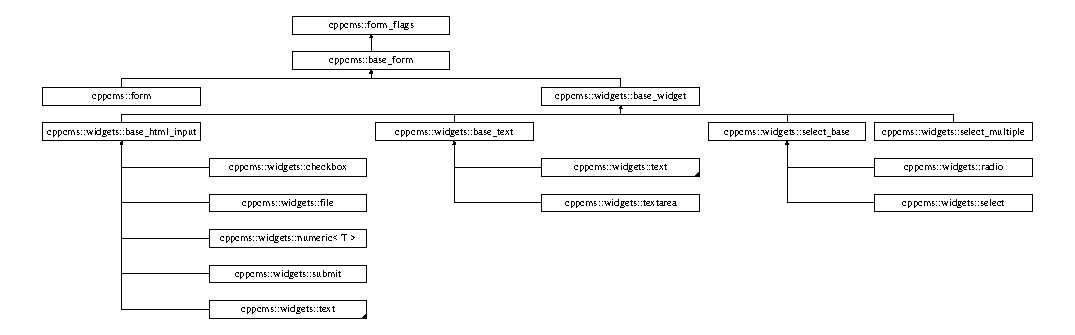
\includegraphics[height=4.057971cm]{classcppcms_1_1base__form}
\end{center}
\end{figure}
\subsection*{Public Member Functions}
\begin{DoxyCompactItemize}
\item 
virtual void {\bf render} ({\bf form\+\_\+context} \&context)=0
\item 
virtual void {\bf load} ({\bf http\+::context} \&context)=0
\item 
virtual bool {\bf validate} ()=0
\item 
virtual void {\bf clear} ()=0
\item 
virtual void {\bf parent} ({\bf base\+\_\+form} $\ast$subform)=0
\item 
virtual {\bf base\+\_\+form} $\ast$ {\bf parent} ()=0
\end{DoxyCompactItemize}
\subsection*{Additional Inherited Members}


\subsection{Detailed Description}
This class is the base class for any form or form widget used in Cpp\+C\+MS. 

It provides basic, abstract operations that every widget or form should implement. 

\subsection{Member Function Documentation}
\index{cppcms\+::base\+\_\+form@{cppcms\+::base\+\_\+form}!clear@{clear}}
\index{clear@{clear}!cppcms\+::base\+\_\+form@{cppcms\+::base\+\_\+form}}
\subsubsection[{clear()=0}]{\setlength{\rightskip}{0pt plus 5cm}virtual void cppcms\+::base\+\_\+form\+::clear (
\begin{DoxyParamCaption}
{}
\end{DoxyParamCaption}
)\hspace{0.3cm}{\ttfamily [pure virtual]}}\label{classcppcms_1_1base__form_a69e995615d0cd577245480eb80ec834a}
Clear the form from all user provided data. 

Implemented in {\bf cppcms\+::widgets\+::select\+\_\+base} \doxyref{}{p.}{classcppcms_1_1widgets_1_1select__base_ac30a6f632f3a423aff9aac4c13d95b6f}, {\bf cppcms\+::widgets\+::select\+\_\+multiple} \doxyref{}{p.}{classcppcms_1_1widgets_1_1select__multiple_a8c4d064583a42de69a9eb6400f446174}, {\bf cppcms\+::widgets\+::numeric$<$ T $>$} \doxyref{}{p.}{classcppcms_1_1widgets_1_1numeric_ac8b010ab4af4e999bc63f8f2d6de782f}, {\bf cppcms\+::widgets\+::base\+\_\+widget} \doxyref{}{p.}{classcppcms_1_1widgets_1_1base__widget_a957f7c7a63f5ea9489b52c3ec1043b81}, and {\bf cppcms\+::form} \doxyref{}{p.}{classcppcms_1_1form_a9c97ed57900d7404396135bbae33b809}.

\index{cppcms\+::base\+\_\+form@{cppcms\+::base\+\_\+form}!load@{load}}
\index{load@{load}!cppcms\+::base\+\_\+form@{cppcms\+::base\+\_\+form}}
\subsubsection[{load(http\+::context \&context)=0}]{\setlength{\rightskip}{0pt plus 5cm}virtual void cppcms\+::base\+\_\+form\+::load (
\begin{DoxyParamCaption}
\item[{{\bf http\+::context} \&}]{context}
\end{DoxyParamCaption}
)\hspace{0.3cm}{\ttfamily [pure virtual]}}\label{classcppcms_1_1base__form_a5f9c5bbfba18076e898ec95827656bc1}
Load the form information from the provided {\tt http\+::context} {\itshape context}. A user can call this function to load all information from the raw P\+O\+S\+T/\+G\+ET data into the internal widget representation. 

Implemented in {\bf cppcms\+::widgets\+::submit} \doxyref{}{p.}{classcppcms_1_1widgets_1_1submit_a9d3c6b1ba7dfc9e1db899dc0067659b1}, {\bf cppcms\+::widgets\+::file} \doxyref{}{p.}{classcppcms_1_1widgets_1_1file_acd5589f0f6a99c6f5590ee2787d407d7}, {\bf cppcms\+::widgets\+::select\+\_\+base} \doxyref{}{p.}{classcppcms_1_1widgets_1_1select__base_a8d41cdd6066ce4e37d937905c5807f5a}, {\bf cppcms\+::widgets\+::select\+\_\+multiple} \doxyref{}{p.}{classcppcms_1_1widgets_1_1select__multiple_aca348bf9b1f56f8ad4bae380275bd03a}, {\bf cppcms\+::widgets\+::checkbox} \doxyref{}{p.}{classcppcms_1_1widgets_1_1checkbox_a07910eeb823fe4ffd4e32fb8c2d0dc54}, {\bf cppcms\+::widgets\+::numeric$<$ T $>$} \doxyref{}{p.}{classcppcms_1_1widgets_1_1numeric_abe1b3a1f4d16f9a56a5dcf8b3bbff0c5}, {\bf cppcms\+::widgets\+::base\+\_\+text} \doxyref{}{p.}{classcppcms_1_1widgets_1_1base__text_a41dc2c33655df59ccdbd680d35793b42}, and {\bf cppcms\+::form} \doxyref{}{p.}{classcppcms_1_1form_a56a59de72f0112b51f068f7511241912}.

\index{cppcms\+::base\+\_\+form@{cppcms\+::base\+\_\+form}!parent@{parent}}
\index{parent@{parent}!cppcms\+::base\+\_\+form@{cppcms\+::base\+\_\+form}}
\subsubsection[{parent(base\+\_\+form $\ast$subform)=0}]{\setlength{\rightskip}{0pt plus 5cm}virtual void cppcms\+::base\+\_\+form\+::parent (
\begin{DoxyParamCaption}
\item[{{\bf base\+\_\+form} $\ast$}]{subform}
\end{DoxyParamCaption}
)\hspace{0.3cm}{\ttfamily [pure virtual]}}\label{classcppcms_1_1base__form_a10c4c5ff417028c72a919740a868bfcd}
Set the parent of this form. Used internally. You should not use it. 

Implemented in {\bf cppcms\+::widgets\+::base\+\_\+widget} \doxyref{}{p.}{classcppcms_1_1widgets_1_1base__widget_aacf20e24298b292a833640e601123a07}, and {\bf cppcms\+::form} \doxyref{}{p.}{classcppcms_1_1form_a969d343a9a2a9db291940c12f3412937}.

\index{cppcms\+::base\+\_\+form@{cppcms\+::base\+\_\+form}!parent@{parent}}
\index{parent@{parent}!cppcms\+::base\+\_\+form@{cppcms\+::base\+\_\+form}}
\subsubsection[{parent()=0}]{\setlength{\rightskip}{0pt plus 5cm}virtual {\bf base\+\_\+form}$\ast$ cppcms\+::base\+\_\+form\+::parent (
\begin{DoxyParamCaption}
{}
\end{DoxyParamCaption}
)\hspace{0.3cm}{\ttfamily [pure virtual]}}\label{classcppcms_1_1base__form_aff998866cd4e17f4c9cf9c7ede1837e5}
Get the parent of this form. If this is the topmost form, N\+U\+LL is returned. 

Implemented in {\bf cppcms\+::widgets\+::base\+\_\+widget} \doxyref{}{p.}{classcppcms_1_1widgets_1_1base__widget_a19bb5e10c4e167d6d3f0056d00387264}, and {\bf cppcms\+::form} \doxyref{}{p.}{classcppcms_1_1form_a78aaad925d3f30b10e5a3ccc80bc88bf}.

\index{cppcms\+::base\+\_\+form@{cppcms\+::base\+\_\+form}!render@{render}}
\index{render@{render}!cppcms\+::base\+\_\+form@{cppcms\+::base\+\_\+form}}
\subsubsection[{render(form\+\_\+context \&context)=0}]{\setlength{\rightskip}{0pt plus 5cm}virtual void cppcms\+::base\+\_\+form\+::render (
\begin{DoxyParamCaption}
\item[{{\bf form\+\_\+context} \&}]{context}
\end{DoxyParamCaption}
)\hspace{0.3cm}{\ttfamily [pure virtual]}}\label{classcppcms_1_1base__form_adb1c6edd653196f575fcacb2aa0fd995}
Render the widget to the output set in {\itshape \doxyref{cppcms\+::form\+\_\+context\+::out()}{p.}{classcppcms_1_1form__context_a2e5e63fa14dd10b59919235ca6ec5f30}} according to the control flags set in {\itshape \doxyref{cppcms\+::form\+\_\+flags}{p.}{structcppcms_1_1form__flags}}. Usually this function is called directly by the template rendering functions. 

Implemented in {\bf cppcms\+::widgets\+::hidden} \doxyref{}{p.}{classcppcms_1_1widgets_1_1hidden_a10e8ebc158a8776c346a567d3f4844df}, {\bf cppcms\+::widgets\+::base\+\_\+widget} \doxyref{}{p.}{classcppcms_1_1widgets_1_1base__widget_a4d62e2342bb41a1b80a2ff0af5c9042b}, and {\bf cppcms\+::form} \doxyref{}{p.}{classcppcms_1_1form_a21c66118d0e80a6496ba2c17baf557b6}.

\index{cppcms\+::base\+\_\+form@{cppcms\+::base\+\_\+form}!validate@{validate}}
\index{validate@{validate}!cppcms\+::base\+\_\+form@{cppcms\+::base\+\_\+form}}
\subsubsection[{validate()=0}]{\setlength{\rightskip}{0pt plus 5cm}virtual bool cppcms\+::base\+\_\+form\+::validate (
\begin{DoxyParamCaption}
{}
\end{DoxyParamCaption}
)\hspace{0.3cm}{\ttfamily [pure virtual]}}\label{classcppcms_1_1base__form_af7d0a7b4c760b43ea3161181906ee4d0}
Validate the form according to defined rules. If all checks are OK, true is returned. If some widget or form fails, false is returned. 

Implemented in {\bf cppcms\+::widgets\+::file} \doxyref{}{p.}{classcppcms_1_1widgets_1_1file_addfa723594f3658578787843fa030486}, {\bf cppcms\+::widgets\+::select\+\_\+base} \doxyref{}{p.}{classcppcms_1_1widgets_1_1select__base_aa2af8d30009d2e366d0608b9503a6551}, {\bf cppcms\+::widgets\+::select\+\_\+multiple} \doxyref{}{p.}{classcppcms_1_1widgets_1_1select__multiple_a0e1c51984aeeb59f5bfa402a5eae2fbf}, {\bf cppcms\+::widgets\+::regex\+\_\+field} \doxyref{}{p.}{classcppcms_1_1widgets_1_1regex__field_a054bf9405d82e1129032b93397ad053e}, {\bf cppcms\+::widgets\+::password} \doxyref{}{p.}{classcppcms_1_1widgets_1_1password_a62059db5f0ff7c43635f2a6ae3455d11}, {\bf cppcms\+::widgets\+::numeric$<$ T $>$} \doxyref{}{p.}{classcppcms_1_1widgets_1_1numeric_a79f8e92aa9991836949978d1b367fe9c}, {\bf cppcms\+::widgets\+::base\+\_\+text} \doxyref{}{p.}{classcppcms_1_1widgets_1_1base__text_a8accbd9e605d1e4dc87337afff6d5b38}, {\bf cppcms\+::widgets\+::base\+\_\+widget} \doxyref{}{p.}{classcppcms_1_1widgets_1_1base__widget_a090169cd0b61fdaceac8ed1b0ca47749}, and {\bf cppcms\+::form} \doxyref{}{p.}{classcppcms_1_1form_a268423c0c006cddde3fea2f6183bf487}.



The documentation for this class was generated from the following file\+:\begin{DoxyCompactItemize}
\item 
cppcms/form.\+h\end{DoxyCompactItemize}

\section{cppcms\+:\+:widgets\+:\+:base\+\_\+html\+\_\+input Class Reference}
\label{classcppcms_1_1widgets_1_1base__html__input}\index{cppcms\+::widgets\+::base\+\_\+html\+\_\+input@{cppcms\+::widgets\+::base\+\_\+html\+\_\+input}}


This class represents a basic widget that generates H\+T\+ML form elements the widgets that use the $<$input \textbackslash{}/$>$ H\+T\+ML tag.  




{\ttfamily \#include $<$cppcms/form.\+h$>$}

Inheritance diagram for cppcms\+:\+:widgets\+:\+:base\+\_\+html\+\_\+input\+:\begin{figure}[H]
\begin{center}
\leavevmode
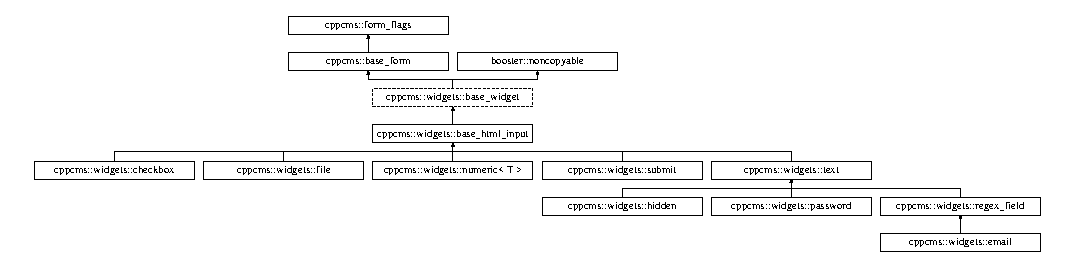
\includegraphics[height=3.156200cm]{classcppcms_1_1widgets_1_1base__html__input}
\end{center}
\end{figure}
\subsection*{Public Member Functions}
\begin{DoxyCompactItemize}
\item 
{\bf base\+\_\+html\+\_\+input} (std\+::string const \&type)
\item 
virtual {\bf $\sim$base\+\_\+html\+\_\+input} ()
\item 
virtual void {\bf render\+\_\+input} ({\bf form\+\_\+context} \&context)
\end{DoxyCompactItemize}
\subsection*{Protected Member Functions}
\begin{DoxyCompactItemize}
\item 
virtual void {\bf render\+\_\+value} ({\bf form\+\_\+context} \&context)=0
\end{DoxyCompactItemize}
\subsection*{Additional Inherited Members}


\subsection{Detailed Description}
This class represents a basic widget that generates H\+T\+ML form elements the widgets that use the $<$input \textbackslash{}/$>$ H\+T\+ML tag. 

It allows you to create your own widgets more easily. It does most of job required to generate the H\+T\+ML. The user is only required to generate the actual value like value=\char`\"{}10.\+34\char`\"{} as with a numeric widget. 

\subsection{Constructor \& Destructor Documentation}
\index{cppcms\+::widgets\+::base\+\_\+html\+\_\+input@{cppcms\+::widgets\+::base\+\_\+html\+\_\+input}!base\+\_\+html\+\_\+input@{base\+\_\+html\+\_\+input}}
\index{base\+\_\+html\+\_\+input@{base\+\_\+html\+\_\+input}!cppcms\+::widgets\+::base\+\_\+html\+\_\+input@{cppcms\+::widgets\+::base\+\_\+html\+\_\+input}}
\subsubsection[{base\+\_\+html\+\_\+input(std\+::string const \&type)}]{\setlength{\rightskip}{0pt plus 5cm}cppcms\+::widgets\+::base\+\_\+html\+\_\+input\+::base\+\_\+html\+\_\+input (
\begin{DoxyParamCaption}
\item[{std\+::string const \&}]{type}
\end{DoxyParamCaption}
)}\label{classcppcms_1_1widgets_1_1base__html__input_aea0331a34cc39f1dd6e3e9f9aaaf3ee6}
Create a new instance. {\itshape type} is the H\+T\+ML type tag of the input element, for example \char`\"{}text\char`\"{} or \char`\"{}password\char`\"{}. \index{cppcms\+::widgets\+::base\+\_\+html\+\_\+input@{cppcms\+::widgets\+::base\+\_\+html\+\_\+input}!````~base\+\_\+html\+\_\+input@{$\sim$base\+\_\+html\+\_\+input}}
\index{````~base\+\_\+html\+\_\+input@{$\sim$base\+\_\+html\+\_\+input}!cppcms\+::widgets\+::base\+\_\+html\+\_\+input@{cppcms\+::widgets\+::base\+\_\+html\+\_\+input}}
\subsubsection[{$\sim$base\+\_\+html\+\_\+input()}]{\setlength{\rightskip}{0pt plus 5cm}virtual cppcms\+::widgets\+::base\+\_\+html\+\_\+input\+::$\sim$base\+\_\+html\+\_\+input (
\begin{DoxyParamCaption}
{}
\end{DoxyParamCaption}
)\hspace{0.3cm}{\ttfamily [virtual]}}\label{classcppcms_1_1widgets_1_1base__html__input_a633a8c103c59270bbd2c6af567f1da23}
Virtual destructor. 

\subsection{Member Function Documentation}
\index{cppcms\+::widgets\+::base\+\_\+html\+\_\+input@{cppcms\+::widgets\+::base\+\_\+html\+\_\+input}!render\+\_\+input@{render\+\_\+input}}
\index{render\+\_\+input@{render\+\_\+input}!cppcms\+::widgets\+::base\+\_\+html\+\_\+input@{cppcms\+::widgets\+::base\+\_\+html\+\_\+input}}
\subsubsection[{render\+\_\+input(form\+\_\+context \&context)}]{\setlength{\rightskip}{0pt plus 5cm}virtual void cppcms\+::widgets\+::base\+\_\+html\+\_\+input\+::render\+\_\+input (
\begin{DoxyParamCaption}
\item[{{\bf form\+\_\+context} \&}]{context}
\end{DoxyParamCaption}
)\hspace{0.3cm}{\ttfamily [virtual]}}\label{classcppcms_1_1widgets_1_1base__html__input_adfab958294d9a6027d0b77c25afba2c1}
This function generates the actual H\+T\+ML. It calls render\+\_\+value where needed. 

Implements {\bf cppcms\+::widgets\+::base\+\_\+widget} \doxyref{}{p.}{classcppcms_1_1widgets_1_1base__widget_a03394613be620bb0d6aeb62818f56b8f}.

\index{cppcms\+::widgets\+::base\+\_\+html\+\_\+input@{cppcms\+::widgets\+::base\+\_\+html\+\_\+input}!render\+\_\+value@{render\+\_\+value}}
\index{render\+\_\+value@{render\+\_\+value}!cppcms\+::widgets\+::base\+\_\+html\+\_\+input@{cppcms\+::widgets\+::base\+\_\+html\+\_\+input}}
\subsubsection[{render\+\_\+value(form\+\_\+context \&context)=0}]{\setlength{\rightskip}{0pt plus 5cm}virtual void cppcms\+::widgets\+::base\+\_\+html\+\_\+input\+::render\+\_\+value (
\begin{DoxyParamCaption}
\item[{{\bf form\+\_\+context} \&}]{context}
\end{DoxyParamCaption}
)\hspace{0.3cm}{\ttfamily [protected]}, {\ttfamily [pure virtual]}}\label{classcppcms_1_1widgets_1_1base__html__input_afd2f99f7dd7b8ebe75e63f1f005068cb}
Write the actual value of the H\+T\+ML tag. Derived classes must implement this. 

Implemented in {\bf cppcms\+::widgets\+::submit} \doxyref{}{p.}{classcppcms_1_1widgets_1_1submit_aeb759bc831400b0ceb964e69ad3d6121}, {\bf cppcms\+::widgets\+::file} \doxyref{}{p.}{classcppcms_1_1widgets_1_1file_aa607511349c879b6e0c1a395f270f76d}, {\bf cppcms\+::widgets\+::checkbox} \doxyref{}{p.}{classcppcms_1_1widgets_1_1checkbox_aace5a796739449ade14f1d203f5d4b7d}, {\bf cppcms\+::widgets\+::numeric$<$ T $>$} \doxyref{}{p.}{classcppcms_1_1widgets_1_1numeric_a81a3fad3834e6d791cc1b173b44ce4ce}, and {\bf cppcms\+::widgets\+::text} \doxyref{}{p.}{classcppcms_1_1widgets_1_1text_acbd7f7a5e7f49e19b73c432232080059}.



The documentation for this class was generated from the following file\+:\begin{DoxyCompactItemize}
\item 
cppcms/form.\+h\end{DoxyCompactItemize}

\section{cppcms\+:\+:widgets\+:\+:base\+\_\+text Class Reference}
\label{classcppcms_1_1widgets_1_1base__text}\index{cppcms\+::widgets\+::base\+\_\+text@{cppcms\+::widgets\+::base\+\_\+text}}


This widget is used as base for text input fields.  




{\ttfamily \#include $<$cppcms/form.\+h$>$}

Inheritance diagram for cppcms\+:\+:widgets\+:\+:base\+\_\+text\+:\begin{figure}[H]
\begin{center}
\leavevmode
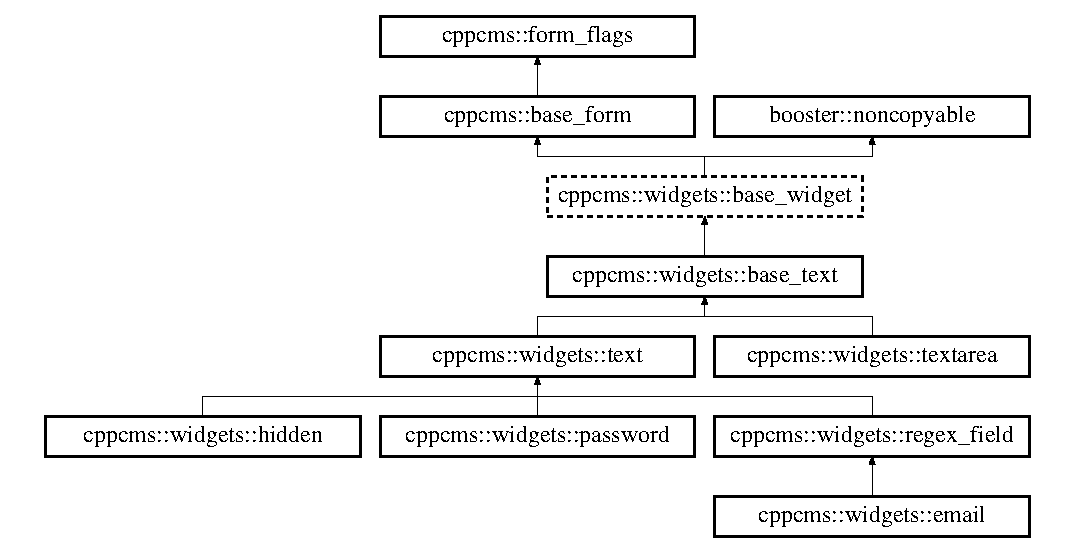
\includegraphics[height=6.987523cm]{classcppcms_1_1widgets_1_1base__text}
\end{center}
\end{figure}
\subsection*{Public Member Functions}
\begin{DoxyCompactItemize}
\item 
std\+::string {\bf value} ()
\item 
void {\bf value} (std\+::string v)
\item 
void {\bf non\+\_\+empty} ()
\item 
void {\bf limits} (int min, int max)
\item 
std\+::pair$<$ int, int $>$ {\bf limits} ()
\item 
void {\bf validate\+\_\+charset} (bool)
\item 
bool {\bf validate\+\_\+charset} ()
\item 
virtual bool {\bf validate} ()
\item 
virtual void {\bf load} ({\bf http\+::context} \&)
\end{DoxyCompactItemize}
\subsection*{Additional Inherited Members}


\subsection{Detailed Description}
This widget is used as base for text input fields. 

This widget is used as the base class for other widgets that are used for text input like\+: \doxyref{text}{p.}{classcppcms_1_1widgets_1_1text}, \doxyref{textarea}{p.}{classcppcms_1_1widgets_1_1textarea}, etc.

This widget does much more than reading simple text data from the P\+O\+ST or G\+ET form. It also performs charset validation. 

\subsection{Member Function Documentation}
\index{cppcms\+::widgets\+::base\+\_\+text@{cppcms\+::widgets\+::base\+\_\+text}!limits@{limits}}
\index{limits@{limits}!cppcms\+::widgets\+::base\+\_\+text@{cppcms\+::widgets\+::base\+\_\+text}}
\subsubsection[{limits(int min, int max)}]{\setlength{\rightskip}{0pt plus 5cm}void cppcms\+::widgets\+::base\+\_\+text\+::limits (
\begin{DoxyParamCaption}
\item[{int}]{min, }
\item[{int}]{max}
\end{DoxyParamCaption}
)}\label{classcppcms_1_1widgets_1_1base__text_a04c3311a56bb10bb5f1b120c586bb58c}
Set the minimum and maximum limits of the text size. Note\+: max == -\/1 indicates that there is no maximum limit; min==0 indicates that there is no minimum limit.

Note\+: these numbers represent the length in Unicode code points (even if the encoding is not Unicode). If the character set validation is disabled, then these numbers represent the number of octets in the string. \index{cppcms\+::widgets\+::base\+\_\+text@{cppcms\+::widgets\+::base\+\_\+text}!limits@{limits}}
\index{limits@{limits}!cppcms\+::widgets\+::base\+\_\+text@{cppcms\+::widgets\+::base\+\_\+text}}
\subsubsection[{limits()}]{\setlength{\rightskip}{0pt plus 5cm}std\+::pair$<$int,int$>$ cppcms\+::widgets\+::base\+\_\+text\+::limits (
\begin{DoxyParamCaption}
{}
\end{DoxyParamCaption}
)}\label{classcppcms_1_1widgets_1_1base__text_a82bd9d00700e3bb77393689cb97cfa97}
Get the minimum and maximum size limits, \index{cppcms\+::widgets\+::base\+\_\+text@{cppcms\+::widgets\+::base\+\_\+text}!load@{load}}
\index{load@{load}!cppcms\+::widgets\+::base\+\_\+text@{cppcms\+::widgets\+::base\+\_\+text}}
\subsubsection[{load(http\+::context \&)}]{\setlength{\rightskip}{0pt plus 5cm}virtual void cppcms\+::widgets\+::base\+\_\+text\+::load (
\begin{DoxyParamCaption}
\item[{{\bf http\+::context} \&}]{}
\end{DoxyParamCaption}
)\hspace{0.3cm}{\ttfamily [virtual]}}\label{classcppcms_1_1widgets_1_1base__text_a41dc2c33655df59ccdbd680d35793b42}
Load the widget for {\tt http\+::context}. It uses the locale given in the context to validate the text. 

Implements {\bf cppcms\+::base\+\_\+form} \doxyref{}{p.}{classcppcms_1_1base__form_a5f9c5bbfba18076e898ec95827656bc1}.

\index{cppcms\+::widgets\+::base\+\_\+text@{cppcms\+::widgets\+::base\+\_\+text}!non\+\_\+empty@{non\+\_\+empty}}
\index{non\+\_\+empty@{non\+\_\+empty}!cppcms\+::widgets\+::base\+\_\+text@{cppcms\+::widgets\+::base\+\_\+text}}
\subsubsection[{non\+\_\+empty()}]{\setlength{\rightskip}{0pt plus 5cm}void cppcms\+::widgets\+::base\+\_\+text\+::non\+\_\+empty (
\begin{DoxyParamCaption}
{}
\end{DoxyParamCaption}
)}\label{classcppcms_1_1widgets_1_1base__text_ad5679b1b2f77fa37ee696ea21c1db8d7}
Inform the validator that this text widget should contain some text. It is similar to limits(1,-\/1). \index{cppcms\+::widgets\+::base\+\_\+text@{cppcms\+::widgets\+::base\+\_\+text}!validate@{validate}}
\index{validate@{validate}!cppcms\+::widgets\+::base\+\_\+text@{cppcms\+::widgets\+::base\+\_\+text}}
\subsubsection[{validate()}]{\setlength{\rightskip}{0pt plus 5cm}virtual bool cppcms\+::widgets\+::base\+\_\+text\+::validate (
\begin{DoxyParamCaption}
{}
\end{DoxyParamCaption}
)\hspace{0.3cm}{\ttfamily [virtual]}}\label{classcppcms_1_1widgets_1_1base__text_a8accbd9e605d1e4dc87337afff6d5b38}
Validate the widget content according to the rules and to the charset encoding.

Notes\+:


\begin{DoxyItemize}
\item The charset validation is very efficient for variable length U\+T\+F-\/8 encoding as well as for most popular fixed length encodings like I\+S\+O-\/8859-\/$\ast$, windows-\/125$\ast$ and koi8$\ast$. For other encodings, character set conversion is used for the actual validation.
\item Special characters (that are not allowed in H\+T\+ML) are assumed to be forbidden, even if they are valid code points (like N\+UL = 0 or D\+EL=127). 
\end{DoxyItemize}

Reimplemented from {\bf cppcms\+::widgets\+::base\+\_\+widget} \doxyref{}{p.}{classcppcms_1_1widgets_1_1base__widget_a090169cd0b61fdaceac8ed1b0ca47749}.



Reimplemented in {\bf cppcms\+::widgets\+::regex\+\_\+field} \doxyref{}{p.}{classcppcms_1_1widgets_1_1regex__field_a054bf9405d82e1129032b93397ad053e}, and {\bf cppcms\+::widgets\+::password} \doxyref{}{p.}{classcppcms_1_1widgets_1_1password_a62059db5f0ff7c43635f2a6ae3455d11}.

\index{cppcms\+::widgets\+::base\+\_\+text@{cppcms\+::widgets\+::base\+\_\+text}!validate\+\_\+charset@{validate\+\_\+charset}}
\index{validate\+\_\+charset@{validate\+\_\+charset}!cppcms\+::widgets\+::base\+\_\+text@{cppcms\+::widgets\+::base\+\_\+text}}
\subsubsection[{validate\+\_\+charset(bool)}]{\setlength{\rightskip}{0pt plus 5cm}void cppcms\+::widgets\+::base\+\_\+text\+::validate\+\_\+charset (
\begin{DoxyParamCaption}
\item[{bool}]{}
\end{DoxyParamCaption}
)}\label{classcppcms_1_1widgets_1_1base__text_a919c491c5ede4da6279d9a14dacd28b5}
Inform the validator whether it should check the validity of the charset. The default is enabled (true).

Generally you should not use this option to disable the charset validation unless you want to load some raw data as form input, or the character set is different from the one defined in the locale. \index{cppcms\+::widgets\+::base\+\_\+text@{cppcms\+::widgets\+::base\+\_\+text}!validate\+\_\+charset@{validate\+\_\+charset}}
\index{validate\+\_\+charset@{validate\+\_\+charset}!cppcms\+::widgets\+::base\+\_\+text@{cppcms\+::widgets\+::base\+\_\+text}}
\subsubsection[{validate\+\_\+charset()}]{\setlength{\rightskip}{0pt plus 5cm}bool cppcms\+::widgets\+::base\+\_\+text\+::validate\+\_\+charset (
\begin{DoxyParamCaption}
{}
\end{DoxyParamCaption}
)}\label{classcppcms_1_1widgets_1_1base__text_a8d95f66180c043bd36bbf104a3f5dfec}
Return true if the charset validation is enabled. \index{cppcms\+::widgets\+::base\+\_\+text@{cppcms\+::widgets\+::base\+\_\+text}!value@{value}}
\index{value@{value}!cppcms\+::widgets\+::base\+\_\+text@{cppcms\+::widgets\+::base\+\_\+text}}
\subsubsection[{value()}]{\setlength{\rightskip}{0pt plus 5cm}std\+::string cppcms\+::widgets\+::base\+\_\+text\+::value (
\begin{DoxyParamCaption}
{}
\end{DoxyParamCaption}
)}\label{classcppcms_1_1widgets_1_1base__text_a465f7cf0e9fee2c9913adf686d1a54f5}
Get the string that contains the input value of the widget. \index{cppcms\+::widgets\+::base\+\_\+text@{cppcms\+::widgets\+::base\+\_\+text}!value@{value}}
\index{value@{value}!cppcms\+::widgets\+::base\+\_\+text@{cppcms\+::widgets\+::base\+\_\+text}}
\subsubsection[{value(std\+::string v)}]{\setlength{\rightskip}{0pt plus 5cm}void cppcms\+::widgets\+::base\+\_\+text\+::value (
\begin{DoxyParamCaption}
\item[{std\+::string}]{v}
\end{DoxyParamCaption}
)}\label{classcppcms_1_1widgets_1_1base__text_aba4241c990dec98201766cc911976838}
Set the widget content to the value {\itshape v} before rendering. 

The documentation for this class was generated from the following file\+:\begin{DoxyCompactItemize}
\item 
cppcms/form.\+h\end{DoxyCompactItemize}

\section{cppcms\+:\+:base\+\_\+view Class Reference}
\label{classcppcms_1_1base__view}\index{cppcms\+::base\+\_\+view@{cppcms\+::base\+\_\+view}}


This class is base class for all views (skins) rendered by Cpp\+C\+MS template engine.  




{\ttfamily \#include $<$cppcms/base\+\_\+view.\+h$>$}

Inheritance diagram for cppcms\+:\+:base\+\_\+view\+:\begin{figure}[H]
\begin{center}
\leavevmode
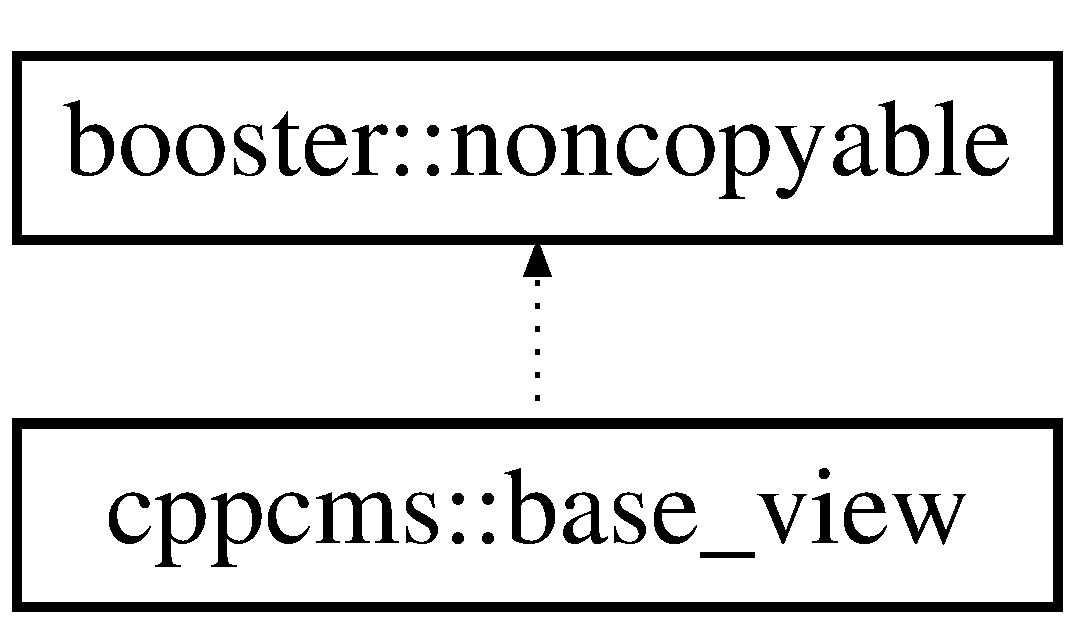
\includegraphics[height=2.000000cm]{classcppcms_1_1base__view}
\end{center}
\end{figure}
\subsection*{Public Member Functions}
\begin{DoxyCompactItemize}
\item 
virtual void {\bf render} ()
\end{DoxyCompactItemize}


\subsection{Detailed Description}
This class is base class for all views (skins) rendered by Cpp\+C\+MS template engine. 

Users are not expected to derive from this class or use it directly. Cpp\+C\+MS template compiler create skins that are usable with template engine and each template is derived from the {\itshape \doxyref{base\+\_\+view}{p.}{classcppcms_1_1base__view}} class. 

\subsection{Member Function Documentation}
\index{cppcms\+::base\+\_\+view@{cppcms\+::base\+\_\+view}!render@{render}}
\index{render@{render}!cppcms\+::base\+\_\+view@{cppcms\+::base\+\_\+view}}
\subsubsection[{render()}]{\setlength{\rightskip}{0pt plus 5cm}virtual void cppcms\+::base\+\_\+view\+::render (
\begin{DoxyParamCaption}
{}
\end{DoxyParamCaption}
)\hspace{0.3cm}{\ttfamily [virtual]}}\label{classcppcms_1_1base__view_ab7d844a52db8bace9f8fc1cd0851a944}
The main rendering function -- render the main H\+T\+ML page. It is usually overridden in template engine. 

The documentation for this class was generated from the following file\+:\begin{DoxyCompactItemize}
\item 
cppcms/base\+\_\+view.\+h\end{DoxyCompactItemize}

\section{cppcms\+:\+:widgets\+:\+:base\+\_\+widget Class Reference}
\label{classcppcms_1_1widgets_1_1base__widget}\index{cppcms\+::widgets\+::base\+\_\+widget@{cppcms\+::widgets\+::base\+\_\+widget}}


this class is the base class of all renderable widgets which can be used with Cpp\+C\+MS form system.  




{\ttfamily \#include $<$cppcms/form.\+h$>$}

Inheritance diagram for cppcms\+:\+:widgets\+:\+:base\+\_\+widget\+:\begin{figure}[H]
\begin{center}
\leavevmode
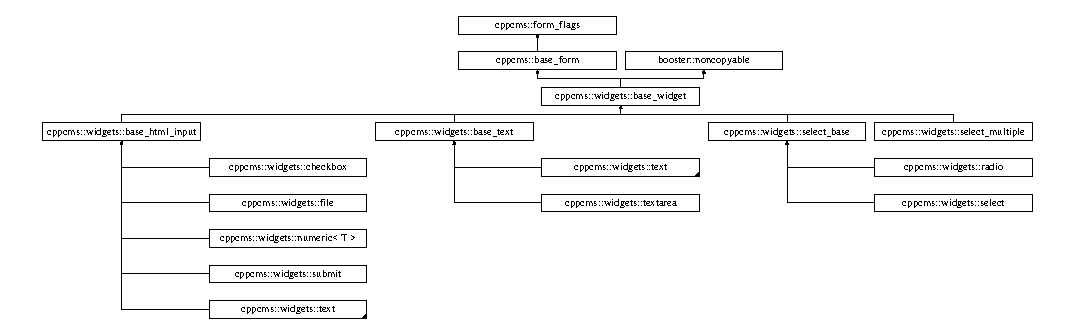
\includegraphics[height=4.057971cm]{classcppcms_1_1widgets_1_1base__widget}
\end{center}
\end{figure}
\subsection*{Public Member Functions}
\begin{DoxyCompactItemize}
\item 
{\bf base\+\_\+widget} ()
\item 
bool {\bf set} ()
\item 
bool {\bf valid} ()
\item 
std\+::string {\bf id} ()
\item 
std\+::string {\bf name} ()
\item 
{\bf locale\+::message} {\bf message} ()
\item 
bool {\bf has\+\_\+message} ()
\item 
{\bf locale\+::message} {\bf error\+\_\+message} ()
\item 
bool {\bf has\+\_\+error\+\_\+message} ()
\item 
{\bf locale\+::message} {\bf help} ()
\item 
bool {\bf has\+\_\+help} ()
\item 
bool {\bf disabled} ()
\item 
void {\bf disabled} (bool)
\item 
bool {\bf readonly} ()
\item 
void {\bf readonly} (bool)
\item 
std\+::string {\bf attributes\+\_\+string} ()
\item 
void {\bf set} (bool)
\item 
void {\bf valid} (bool)
\item 
void {\bf id} (std\+::string)
\item 
void {\bf name} (std\+::string)
\item 
void {\bf message} (std\+::string)
\item 
void {\bf message} ({\bf locale\+::message} const \&)
\item 
void {\bf error\+\_\+message} (std\+::string)
\item 
void {\bf error\+\_\+message} ({\bf locale\+::message} const \&)
\item 
void {\bf help} (std\+::string)
\item 
void {\bf help} ({\bf locale\+::message} const \&msg)
\item 
void {\bf attributes\+\_\+string} (std\+::string v)
\item 
virtual void {\bf render} ({\bf form\+\_\+context} \&context)
\item 
virtual void {\bf render\+\_\+input} ({\bf form\+\_\+context} \&context)=0
\item 
virtual void {\bf clear} ()
\item 
virtual bool {\bf validate} ()
\item 
virtual void {\bf render\+\_\+attributes} ({\bf form\+\_\+context} \&context)
\item 
virtual void {\bf parent} ({\bf base\+\_\+form} $\ast$subform)
\item 
virtual {\bf form} $\ast$ {\bf parent} ()
\item 
void {\bf pre\+\_\+load} ({\bf http\+::context} \&)
\end{DoxyCompactItemize}
\subsection*{Protected Member Functions}
\begin{DoxyCompactItemize}
\item 
void {\bf auto\+\_\+generate} ({\bf form\+\_\+context} $\ast$context=0)
\end{DoxyCompactItemize}
\subsection*{Additional Inherited Members}


\subsection{Detailed Description}
this class is the base class of all renderable widgets which can be used with Cpp\+C\+MS form system. 

All cppcms widgets are derived from this class. Users who want to create their own custom widgets must derive them from this class. 

\subsection{Constructor \& Destructor Documentation}
\index{cppcms\+::widgets\+::base\+\_\+widget@{cppcms\+::widgets\+::base\+\_\+widget}!base\+\_\+widget@{base\+\_\+widget}}
\index{base\+\_\+widget@{base\+\_\+widget}!cppcms\+::widgets\+::base\+\_\+widget@{cppcms\+::widgets\+::base\+\_\+widget}}
\subsubsection[{base\+\_\+widget()}]{\setlength{\rightskip}{0pt plus 5cm}cppcms\+::widgets\+::base\+\_\+widget\+::base\+\_\+widget (
\begin{DoxyParamCaption}
{}
\end{DoxyParamCaption}
)}\label{classcppcms_1_1widgets_1_1base__widget_a2ac4411c0e621b40e28b0c3da8226515}
Default constructor. 

\subsection{Member Function Documentation}
\index{cppcms\+::widgets\+::base\+\_\+widget@{cppcms\+::widgets\+::base\+\_\+widget}!attributes\+\_\+string@{attributes\+\_\+string}}
\index{attributes\+\_\+string@{attributes\+\_\+string}!cppcms\+::widgets\+::base\+\_\+widget@{cppcms\+::widgets\+::base\+\_\+widget}}
\subsubsection[{attributes\+\_\+string()}]{\setlength{\rightskip}{0pt plus 5cm}std\+::string cppcms\+::widgets\+::base\+\_\+widget\+::attributes\+\_\+string (
\begin{DoxyParamCaption}
{}
\end{DoxyParamCaption}
)}\label{classcppcms_1_1widgets_1_1base__widget_ad91d5bafd0f677f194b021f6e1462fe6}
Get the general user defined attribute string that can be added to the widget. \index{cppcms\+::widgets\+::base\+\_\+widget@{cppcms\+::widgets\+::base\+\_\+widget}!attributes\+\_\+string@{attributes\+\_\+string}}
\index{attributes\+\_\+string@{attributes\+\_\+string}!cppcms\+::widgets\+::base\+\_\+widget@{cppcms\+::widgets\+::base\+\_\+widget}}
\subsubsection[{attributes\+\_\+string(std\+::string v)}]{\setlength{\rightskip}{0pt plus 5cm}void cppcms\+::widgets\+::base\+\_\+widget\+::attributes\+\_\+string (
\begin{DoxyParamCaption}
\item[{std\+::string}]{v}
\end{DoxyParamCaption}
)}\label{classcppcms_1_1widgets_1_1base__widget_a61f4235facbbeae2221cc3341692816a}
Set general H\+T\+ML attributes that are not directly supported For example\+:


\begin{DoxyCode}
my\_widget.attributes\_string(\textcolor{stringliteral}{"style='direction:rtl' onclick='return foo()'"});
\end{DoxyCode}


This string is inserted as-\/is just after render\+\_\+input\+\_\+start. \index{cppcms\+::widgets\+::base\+\_\+widget@{cppcms\+::widgets\+::base\+\_\+widget}!auto\+\_\+generate@{auto\+\_\+generate}}
\index{auto\+\_\+generate@{auto\+\_\+generate}!cppcms\+::widgets\+::base\+\_\+widget@{cppcms\+::widgets\+::base\+\_\+widget}}
\subsubsection[{auto\+\_\+generate(form\+\_\+context $\ast$context=0)}]{\setlength{\rightskip}{0pt plus 5cm}void cppcms\+::widgets\+::base\+\_\+widget\+::auto\+\_\+generate (
\begin{DoxyParamCaption}
\item[{{\bf form\+\_\+context} $\ast$}]{context = {\ttfamily 0}}
\end{DoxyParamCaption}
)\hspace{0.3cm}{\ttfamily [protected]}}\label{classcppcms_1_1widgets_1_1base__widget_ac5095a05367edccbf09f494d9d6db5e6}
This function should be called by overloadeding the load/render methods before the loading/rendering starts. \index{cppcms\+::widgets\+::base\+\_\+widget@{cppcms\+::widgets\+::base\+\_\+widget}!clear@{clear}}
\index{clear@{clear}!cppcms\+::widgets\+::base\+\_\+widget@{cppcms\+::widgets\+::base\+\_\+widget}}
\subsubsection[{clear()}]{\setlength{\rightskip}{0pt plus 5cm}virtual void cppcms\+::widgets\+::base\+\_\+widget\+::clear (
\begin{DoxyParamCaption}
{}
\end{DoxyParamCaption}
)\hspace{0.3cm}{\ttfamily [virtual]}}\label{classcppcms_1_1widgets_1_1base__widget_a957f7c7a63f5ea9489b52c3ec1043b81}
Clear the form. It also calls set(false). 

Implements {\bf cppcms\+::base\+\_\+form} \doxyref{}{p.}{classcppcms_1_1base__form_a69e995615d0cd577245480eb80ec834a}.



Reimplemented in {\bf cppcms\+::widgets\+::select\+\_\+base} \doxyref{}{p.}{classcppcms_1_1widgets_1_1select__base_ac30a6f632f3a423aff9aac4c13d95b6f}, {\bf cppcms\+::widgets\+::select\+\_\+multiple} \doxyref{}{p.}{classcppcms_1_1widgets_1_1select__multiple_a8c4d064583a42de69a9eb6400f446174}, and {\bf cppcms\+::widgets\+::numeric$<$ T $>$} \doxyref{}{p.}{classcppcms_1_1widgets_1_1numeric_ac8b010ab4af4e999bc63f8f2d6de782f}.

\index{cppcms\+::widgets\+::base\+\_\+widget@{cppcms\+::widgets\+::base\+\_\+widget}!disabled@{disabled}}
\index{disabled@{disabled}!cppcms\+::widgets\+::base\+\_\+widget@{cppcms\+::widgets\+::base\+\_\+widget}}
\subsubsection[{disabled()}]{\setlength{\rightskip}{0pt plus 5cm}bool cppcms\+::widgets\+::base\+\_\+widget\+::disabled (
\begin{DoxyParamCaption}
{}
\end{DoxyParamCaption}
)}\label{classcppcms_1_1widgets_1_1base__widget_a1c13127fbab256250251ad47f2d94dd4}
Get the H\+T\+ML {\ttfamily disabled} attribute. \index{cppcms\+::widgets\+::base\+\_\+widget@{cppcms\+::widgets\+::base\+\_\+widget}!disabled@{disabled}}
\index{disabled@{disabled}!cppcms\+::widgets\+::base\+\_\+widget@{cppcms\+::widgets\+::base\+\_\+widget}}
\subsubsection[{disabled(bool)}]{\setlength{\rightskip}{0pt plus 5cm}void cppcms\+::widgets\+::base\+\_\+widget\+::disabled (
\begin{DoxyParamCaption}
\item[{bool}]{}
\end{DoxyParamCaption}
)}\label{classcppcms_1_1widgets_1_1base__widget_a8ef75516b30690b1fd0bdd36784ab55c}
Set/\+Unset the H\+T\+ML {\ttfamily disabled} attribute. \index{cppcms\+::widgets\+::base\+\_\+widget@{cppcms\+::widgets\+::base\+\_\+widget}!error\+\_\+message@{error\+\_\+message}}
\index{error\+\_\+message@{error\+\_\+message}!cppcms\+::widgets\+::base\+\_\+widget@{cppcms\+::widgets\+::base\+\_\+widget}}
\subsubsection[{error\+\_\+message()}]{\setlength{\rightskip}{0pt plus 5cm}{\bf locale\+::message} cppcms\+::widgets\+::base\+\_\+widget\+::error\+\_\+message (
\begin{DoxyParamCaption}
{}
\end{DoxyParamCaption}
)}\label{classcppcms_1_1widgets_1_1base__widget_a7bcf3d357b3112d492bb7dd0d021e483}
Get the error message that would be displayed near the widget if the widget validation failed. \index{cppcms\+::widgets\+::base\+\_\+widget@{cppcms\+::widgets\+::base\+\_\+widget}!error\+\_\+message@{error\+\_\+message}}
\index{error\+\_\+message@{error\+\_\+message}!cppcms\+::widgets\+::base\+\_\+widget@{cppcms\+::widgets\+::base\+\_\+widget}}
\subsubsection[{error\+\_\+message(std\+::string)}]{\setlength{\rightskip}{0pt plus 5cm}void cppcms\+::widgets\+::base\+\_\+widget\+::error\+\_\+message (
\begin{DoxyParamCaption}
\item[{std\+::string}]{}
\end{DoxyParamCaption}
)}\label{classcppcms_1_1widgets_1_1base__widget_af18b8ac8a1bf73da6818a3d5449e5987}
Set the error message that is displayed for invalid widgets.

If it is not set, a simple \char`\"{}$\ast$\char`\"{} is shown instead. \index{cppcms\+::widgets\+::base\+\_\+widget@{cppcms\+::widgets\+::base\+\_\+widget}!error\+\_\+message@{error\+\_\+message}}
\index{error\+\_\+message@{error\+\_\+message}!cppcms\+::widgets\+::base\+\_\+widget@{cppcms\+::widgets\+::base\+\_\+widget}}
\subsubsection[{error\+\_\+message(locale\+::message const \&)}]{\setlength{\rightskip}{0pt plus 5cm}void cppcms\+::widgets\+::base\+\_\+widget\+::error\+\_\+message (
\begin{DoxyParamCaption}
\item[{{\bf locale\+::message} const \&}]{}
\end{DoxyParamCaption}
)}\label{classcppcms_1_1widgets_1_1base__widget_a9c8e5ab2f264dbb4534d9c53ca1103be}
Set the translatable error message that is displayed for invalid widgets.

If it is not set, a simple \char`\"{}$\ast$\char`\"{} is shown instead. \index{cppcms\+::widgets\+::base\+\_\+widget@{cppcms\+::widgets\+::base\+\_\+widget}!has\+\_\+error\+\_\+message@{has\+\_\+error\+\_\+message}}
\index{has\+\_\+error\+\_\+message@{has\+\_\+error\+\_\+message}!cppcms\+::widgets\+::base\+\_\+widget@{cppcms\+::widgets\+::base\+\_\+widget}}
\subsubsection[{has\+\_\+error\+\_\+message()}]{\setlength{\rightskip}{0pt plus 5cm}bool cppcms\+::widgets\+::base\+\_\+widget\+::has\+\_\+error\+\_\+message (
\begin{DoxyParamCaption}
{}
\end{DoxyParamCaption}
)}\label{classcppcms_1_1widgets_1_1base__widget_a2fc78787d3a15200b0436c00647f5299}
Check if an error message is set. \index{cppcms\+::widgets\+::base\+\_\+widget@{cppcms\+::widgets\+::base\+\_\+widget}!has\+\_\+help@{has\+\_\+help}}
\index{has\+\_\+help@{has\+\_\+help}!cppcms\+::widgets\+::base\+\_\+widget@{cppcms\+::widgets\+::base\+\_\+widget}}
\subsubsection[{has\+\_\+help()}]{\setlength{\rightskip}{0pt plus 5cm}bool cppcms\+::widgets\+::base\+\_\+widget\+::has\+\_\+help (
\begin{DoxyParamCaption}
{}
\end{DoxyParamCaption}
)}\label{classcppcms_1_1widgets_1_1base__widget_a2932b7d598bf2d9cc34583c87ca625a3}
Check if a help message is set. \index{cppcms\+::widgets\+::base\+\_\+widget@{cppcms\+::widgets\+::base\+\_\+widget}!has\+\_\+message@{has\+\_\+message}}
\index{has\+\_\+message@{has\+\_\+message}!cppcms\+::widgets\+::base\+\_\+widget@{cppcms\+::widgets\+::base\+\_\+widget}}
\subsubsection[{has\+\_\+message()}]{\setlength{\rightskip}{0pt plus 5cm}bool cppcms\+::widgets\+::base\+\_\+widget\+::has\+\_\+message (
\begin{DoxyParamCaption}
{}
\end{DoxyParamCaption}
)}\label{classcppcms_1_1widgets_1_1base__widget_a3166e364657999977accbaacef547c49}
Check if a message is set. \index{cppcms\+::widgets\+::base\+\_\+widget@{cppcms\+::widgets\+::base\+\_\+widget}!help@{help}}
\index{help@{help}!cppcms\+::widgets\+::base\+\_\+widget@{cppcms\+::widgets\+::base\+\_\+widget}}
\subsubsection[{help()}]{\setlength{\rightskip}{0pt plus 5cm}{\bf locale\+::message} cppcms\+::widgets\+::base\+\_\+widget\+::help (
\begin{DoxyParamCaption}
{}
\end{DoxyParamCaption}
)}\label{classcppcms_1_1widgets_1_1base__widget_a11bcfe32677465e651686556d6b0fc4f}
Get the eventual long description of the wigget. \index{cppcms\+::widgets\+::base\+\_\+widget@{cppcms\+::widgets\+::base\+\_\+widget}!help@{help}}
\index{help@{help}!cppcms\+::widgets\+::base\+\_\+widget@{cppcms\+::widgets\+::base\+\_\+widget}}
\subsubsection[{help(std\+::string)}]{\setlength{\rightskip}{0pt plus 5cm}void cppcms\+::widgets\+::base\+\_\+widget\+::help (
\begin{DoxyParamCaption}
\item[{std\+::string}]{}
\end{DoxyParamCaption}
)}\label{classcppcms_1_1widgets_1_1base__widget_a4ec743c4910b39fd4de28bbed5f0fa33}
Set a longer help message that describes this widget. \index{cppcms\+::widgets\+::base\+\_\+widget@{cppcms\+::widgets\+::base\+\_\+widget}!help@{help}}
\index{help@{help}!cppcms\+::widgets\+::base\+\_\+widget@{cppcms\+::widgets\+::base\+\_\+widget}}
\subsubsection[{help(locale\+::message const \&msg)}]{\setlength{\rightskip}{0pt plus 5cm}void cppcms\+::widgets\+::base\+\_\+widget\+::help (
\begin{DoxyParamCaption}
\item[{{\bf locale\+::message} const \&}]{msg}
\end{DoxyParamCaption}
)}\label{classcppcms_1_1widgets_1_1base__widget_a35d76aab23f4f067bb575c8bf03fa11c}
Set a translatable help message that describes this widget. \index{cppcms\+::widgets\+::base\+\_\+widget@{cppcms\+::widgets\+::base\+\_\+widget}!id@{id}}
\index{id@{id}!cppcms\+::widgets\+::base\+\_\+widget@{cppcms\+::widgets\+::base\+\_\+widget}}
\subsubsection[{id()}]{\setlength{\rightskip}{0pt plus 5cm}std\+::string cppcms\+::widgets\+::base\+\_\+widget\+::id (
\begin{DoxyParamCaption}
{}
\end{DoxyParamCaption}
)}\label{classcppcms_1_1widgets_1_1base__widget_aca2eb9140d6900f140e4bdfada731776}
Get the H\+T\+ML {\itshape id} attribute. \index{cppcms\+::widgets\+::base\+\_\+widget@{cppcms\+::widgets\+::base\+\_\+widget}!id@{id}}
\index{id@{id}!cppcms\+::widgets\+::base\+\_\+widget@{cppcms\+::widgets\+::base\+\_\+widget}}
\subsubsection[{id(std\+::string)}]{\setlength{\rightskip}{0pt plus 5cm}void cppcms\+::widgets\+::base\+\_\+widget\+::id (
\begin{DoxyParamCaption}
\item[{std\+::string}]{}
\end{DoxyParamCaption}
)}\label{classcppcms_1_1widgets_1_1base__widget_a400e8416cfbe4826665dd7f84db1422c}
Set the H\+T\+ML {\ttfamily id} attribute of the widget. \index{cppcms\+::widgets\+::base\+\_\+widget@{cppcms\+::widgets\+::base\+\_\+widget}!message@{message}}
\index{message@{message}!cppcms\+::widgets\+::base\+\_\+widget@{cppcms\+::widgets\+::base\+\_\+widget}}
\subsubsection[{message()}]{\setlength{\rightskip}{0pt plus 5cm}{\bf locale\+::message} cppcms\+::widgets\+::base\+\_\+widget\+::message (
\begin{DoxyParamCaption}
{}
\end{DoxyParamCaption}
)}\label{classcppcms_1_1widgets_1_1base__widget_aa18b1b80d669e94e86a96efa3a86a4f3}
Get the short message that would be displayed near the widget. \index{cppcms\+::widgets\+::base\+\_\+widget@{cppcms\+::widgets\+::base\+\_\+widget}!message@{message}}
\index{message@{message}!cppcms\+::widgets\+::base\+\_\+widget@{cppcms\+::widgets\+::base\+\_\+widget}}
\subsubsection[{message(std\+::string)}]{\setlength{\rightskip}{0pt plus 5cm}void cppcms\+::widgets\+::base\+\_\+widget\+::message (
\begin{DoxyParamCaption}
\item[{std\+::string}]{}
\end{DoxyParamCaption}
)}\label{classcppcms_1_1widgets_1_1base__widget_a3d966eee8ee87cc284a3a4c781b22bc4}
Set a short description for the widget. Generally, it is a good idea to define this value.

The short message can also be set using the \doxyref{base\+\_\+widget}{p.}{classcppcms_1_1widgets_1_1base__widget} constructor. \index{cppcms\+::widgets\+::base\+\_\+widget@{cppcms\+::widgets\+::base\+\_\+widget}!message@{message}}
\index{message@{message}!cppcms\+::widgets\+::base\+\_\+widget@{cppcms\+::widgets\+::base\+\_\+widget}}
\subsubsection[{message(locale\+::message const \&)}]{\setlength{\rightskip}{0pt plus 5cm}void cppcms\+::widgets\+::base\+\_\+widget\+::message (
\begin{DoxyParamCaption}
\item[{{\bf locale\+::message} const \&}]{}
\end{DoxyParamCaption}
)}\label{classcppcms_1_1widgets_1_1base__widget_a2d9b4c43b109f74c3daf514ad8510a0c}
Set a short translatable description for the widget. Generally, it is a good idea to define this value.

The short message can also be set using the \doxyref{base\+\_\+widget}{p.}{classcppcms_1_1widgets_1_1base__widget} constructor. \index{cppcms\+::widgets\+::base\+\_\+widget@{cppcms\+::widgets\+::base\+\_\+widget}!name@{name}}
\index{name@{name}!cppcms\+::widgets\+::base\+\_\+widget@{cppcms\+::widgets\+::base\+\_\+widget}}
\subsubsection[{name()}]{\setlength{\rightskip}{0pt plus 5cm}std\+::string cppcms\+::widgets\+::base\+\_\+widget\+::name (
\begin{DoxyParamCaption}
{}
\end{DoxyParamCaption}
)}\label{classcppcms_1_1widgets_1_1base__widget_a1c530e58db8631a1da3875e05ada174b}
Get the H\+T\+ML {\itshape name} attribute. \index{cppcms\+::widgets\+::base\+\_\+widget@{cppcms\+::widgets\+::base\+\_\+widget}!name@{name}}
\index{name@{name}!cppcms\+::widgets\+::base\+\_\+widget@{cppcms\+::widgets\+::base\+\_\+widget}}
\subsubsection[{name(std\+::string)}]{\setlength{\rightskip}{0pt plus 5cm}void cppcms\+::widgets\+::base\+\_\+widget\+::name (
\begin{DoxyParamCaption}
\item[{std\+::string}]{}
\end{DoxyParamCaption}
)}\label{classcppcms_1_1widgets_1_1base__widget_af3f99c2708986a4b5dadf35d6f1c7744}
Set the H\+T\+ML {\ttfamily name} attribute of the widget. Note\+: if this attribute is not set, the widget will not be able to be loaded from the P\+O\+S\+T/\+G\+ET data. \index{cppcms\+::widgets\+::base\+\_\+widget@{cppcms\+::widgets\+::base\+\_\+widget}!parent@{parent}}
\index{parent@{parent}!cppcms\+::widgets\+::base\+\_\+widget@{cppcms\+::widgets\+::base\+\_\+widget}}
\subsubsection[{parent(base\+\_\+form $\ast$subform)}]{\setlength{\rightskip}{0pt plus 5cm}virtual void cppcms\+::widgets\+::base\+\_\+widget\+::parent (
\begin{DoxyParamCaption}
\item[{{\bf base\+\_\+form} $\ast$}]{subform}
\end{DoxyParamCaption}
)\hspace{0.3cm}{\ttfamily [virtual]}}\label{classcppcms_1_1widgets_1_1base__widget_aacf20e24298b292a833640e601123a07}
Set the parent of this widget. It is used internally; you should not use it. It is called when the form is added or attached to another form. 

Implements {\bf cppcms\+::base\+\_\+form} \doxyref{}{p.}{classcppcms_1_1base__form_a10c4c5ff417028c72a919740a868bfcd}.

\index{cppcms\+::widgets\+::base\+\_\+widget@{cppcms\+::widgets\+::base\+\_\+widget}!parent@{parent}}
\index{parent@{parent}!cppcms\+::widgets\+::base\+\_\+widget@{cppcms\+::widgets\+::base\+\_\+widget}}
\subsubsection[{parent()}]{\setlength{\rightskip}{0pt plus 5cm}virtual {\bf form}$\ast$ cppcms\+::widgets\+::base\+\_\+widget\+::parent (
\begin{DoxyParamCaption}
{}
\end{DoxyParamCaption}
)\hspace{0.3cm}{\ttfamily [virtual]}}\label{classcppcms_1_1widgets_1_1base__widget_a19bb5e10c4e167d6d3f0056d00387264}
Get the parent of this form. If this is the topmost form, N\+U\+LL is returned. It is assumed that the parent is always a form. 

Implements {\bf cppcms\+::base\+\_\+form} \doxyref{}{p.}{classcppcms_1_1base__form_aff998866cd4e17f4c9cf9c7ede1837e5}.

\index{cppcms\+::widgets\+::base\+\_\+widget@{cppcms\+::widgets\+::base\+\_\+widget}!pre\+\_\+load@{pre\+\_\+load}}
\index{pre\+\_\+load@{pre\+\_\+load}!cppcms\+::widgets\+::base\+\_\+widget@{cppcms\+::widgets\+::base\+\_\+widget}}
\subsubsection[{pre\+\_\+load(http\+::context \&)}]{\setlength{\rightskip}{0pt plus 5cm}void cppcms\+::widgets\+::base\+\_\+widget\+::pre\+\_\+load (
\begin{DoxyParamCaption}
\item[{{\bf http\+::context} \&}]{}
\end{DoxyParamCaption}
)}\label{classcppcms_1_1widgets_1_1base__widget_ad62dc6a5b2fd15aeebdcff8656056459}
This function should be called before actual loading of widgets, it performs cross widgets validation and causes automatic generation of undefined names \index{cppcms\+::widgets\+::base\+\_\+widget@{cppcms\+::widgets\+::base\+\_\+widget}!readonly@{readonly}}
\index{readonly@{readonly}!cppcms\+::widgets\+::base\+\_\+widget@{cppcms\+::widgets\+::base\+\_\+widget}}
\subsubsection[{readonly()}]{\setlength{\rightskip}{0pt plus 5cm}bool cppcms\+::widgets\+::base\+\_\+widget\+::readonly (
\begin{DoxyParamCaption}
{}
\end{DoxyParamCaption}
)}\label{classcppcms_1_1widgets_1_1base__widget_af4bc7448ae98c35a54eaf7bc31b01bc6}
Get the H\+T\+ML {\ttfamily readonly} attribute.

\doxyref{New in Cpp\+C\+MS 1.\+2}{p.}{v1_2} \index{cppcms\+::widgets\+::base\+\_\+widget@{cppcms\+::widgets\+::base\+\_\+widget}!readonly@{readonly}}
\index{readonly@{readonly}!cppcms\+::widgets\+::base\+\_\+widget@{cppcms\+::widgets\+::base\+\_\+widget}}
\subsubsection[{readonly(bool)}]{\setlength{\rightskip}{0pt plus 5cm}void cppcms\+::widgets\+::base\+\_\+widget\+::readonly (
\begin{DoxyParamCaption}
\item[{bool}]{}
\end{DoxyParamCaption}
)}\label{classcppcms_1_1widgets_1_1base__widget_a916056f9d8968439bc2c51ea414894d9}
Set/\+Unset the H\+T\+ML {\ttfamily readonly} attribute.

\doxyref{New in Cpp\+C\+MS 1.\+2}{p.}{v1_2} \index{cppcms\+::widgets\+::base\+\_\+widget@{cppcms\+::widgets\+::base\+\_\+widget}!render@{render}}
\index{render@{render}!cppcms\+::widgets\+::base\+\_\+widget@{cppcms\+::widgets\+::base\+\_\+widget}}
\subsubsection[{render(form\+\_\+context \&context)}]{\setlength{\rightskip}{0pt plus 5cm}virtual void cppcms\+::widgets\+::base\+\_\+widget\+::render (
\begin{DoxyParamCaption}
\item[{{\bf form\+\_\+context} \&}]{context}
\end{DoxyParamCaption}
)\hspace{0.3cm}{\ttfamily [virtual]}}\label{classcppcms_1_1widgets_1_1base__widget_a4d62e2342bb41a1b80a2ff0af5c9042b}
Render the full widget together with error messages and decorations as paragraphs or table elements to the output set in {\itshape \doxyref{cppcms\+::form\+\_\+context\+::out()}{p.}{classcppcms_1_1form__context_a2e5e63fa14dd10b59919235ca6ec5f30}}. 

Implements {\bf cppcms\+::base\+\_\+form} \doxyref{}{p.}{classcppcms_1_1base__form_adb1c6edd653196f575fcacb2aa0fd995}.



Reimplemented in {\bf cppcms\+::widgets\+::hidden} \doxyref{}{p.}{classcppcms_1_1widgets_1_1hidden_a10e8ebc158a8776c346a567d3f4844df}.

\index{cppcms\+::widgets\+::base\+\_\+widget@{cppcms\+::widgets\+::base\+\_\+widget}!render\+\_\+attributes@{render\+\_\+attributes}}
\index{render\+\_\+attributes@{render\+\_\+attributes}!cppcms\+::widgets\+::base\+\_\+widget@{cppcms\+::widgets\+::base\+\_\+widget}}
\subsubsection[{render\+\_\+attributes(form\+\_\+context \&context)}]{\setlength{\rightskip}{0pt plus 5cm}virtual void cppcms\+::widgets\+::base\+\_\+widget\+::render\+\_\+attributes (
\begin{DoxyParamCaption}
\item[{{\bf form\+\_\+context} \&}]{context}
\end{DoxyParamCaption}
)\hspace{0.3cm}{\ttfamily [virtual]}}\label{classcppcms_1_1widgets_1_1base__widget_a6f0354040920a70e3248c94d357774f0}
Render standard common attributes like {\itshape id}, {\itshape name}, {\itshape disabled}, etc. 

Reimplemented in {\bf cppcms\+::widgets\+::text} \doxyref{}{p.}{classcppcms_1_1widgets_1_1text_a5d71259184320fc4a11819cebe2a0154}.

\index{cppcms\+::widgets\+::base\+\_\+widget@{cppcms\+::widgets\+::base\+\_\+widget}!render\+\_\+input@{render\+\_\+input}}
\index{render\+\_\+input@{render\+\_\+input}!cppcms\+::widgets\+::base\+\_\+widget@{cppcms\+::widgets\+::base\+\_\+widget}}
\subsubsection[{render\+\_\+input(form\+\_\+context \&context)=0}]{\setlength{\rightskip}{0pt plus 5cm}virtual void cppcms\+::widgets\+::base\+\_\+widget\+::render\+\_\+input (
\begin{DoxyParamCaption}
\item[{{\bf form\+\_\+context} \&}]{context}
\end{DoxyParamCaption}
)\hspace{0.3cm}{\ttfamily [pure virtual]}}\label{classcppcms_1_1widgets_1_1base__widget_a03394613be620bb0d6aeb62818f56b8f}
This is a virtual member function that should be implemented by each widget. It executes the actual rendering of the H\+T\+ML form. 

Implemented in {\bf cppcms\+::widgets\+::radio} \doxyref{}{p.}{classcppcms_1_1widgets_1_1radio_ae34173f78d1df5ac05053b5349b03131}, {\bf cppcms\+::widgets\+::select} \doxyref{}{p.}{classcppcms_1_1widgets_1_1select_a4bced34474dcca17418fd20a21d4b529}, {\bf cppcms\+::widgets\+::select\+\_\+base} \doxyref{}{p.}{classcppcms_1_1widgets_1_1select__base_ab1119401ddea3d4beb266e8a7cb9afee}, {\bf cppcms\+::widgets\+::select\+\_\+multiple} \doxyref{}{p.}{classcppcms_1_1widgets_1_1select__multiple_aa31c3a9b5fb0cd21aae7e4e85e797433}, {\bf cppcms\+::widgets\+::textarea} \doxyref{}{p.}{classcppcms_1_1widgets_1_1textarea_ac7fac283b705a87071f013edd286ed31}, and {\bf cppcms\+::widgets\+::base\+\_\+html\+\_\+input} \doxyref{}{p.}{classcppcms_1_1widgets_1_1base__html__input_adfab958294d9a6027d0b77c25afba2c1}.

\index{cppcms\+::widgets\+::base\+\_\+widget@{cppcms\+::widgets\+::base\+\_\+widget}!set@{set}}
\index{set@{set}!cppcms\+::widgets\+::base\+\_\+widget@{cppcms\+::widgets\+::base\+\_\+widget}}
\subsubsection[{set()}]{\setlength{\rightskip}{0pt plus 5cm}bool cppcms\+::widgets\+::base\+\_\+widget\+::set (
\begin{DoxyParamCaption}
{}
\end{DoxyParamCaption}
)}\label{classcppcms_1_1widgets_1_1base__widget_afd814f0d448866c0f316e38e05fc8d3f}
Check if a value has been assigned to the widget. It is usually true when the user has assigned a value to the widget or when the widget is loaded.

If there is a reasonable default value for the widget then \doxyref{set()}{p.}{classcppcms_1_1widgets_1_1base__widget_afd814f0d448866c0f316e38e05fc8d3f} should be true. For widgets like file or numeric where explicit parsing is required, the \doxyref{set()}{p.}{classcppcms_1_1widgets_1_1base__widget_afd814f0d448866c0f316e38e05fc8d3f} value would indicate that user provided some value (i.\+e. uploaded a file or entered a number). \index{cppcms\+::widgets\+::base\+\_\+widget@{cppcms\+::widgets\+::base\+\_\+widget}!set@{set}}
\index{set@{set}!cppcms\+::widgets\+::base\+\_\+widget@{cppcms\+::widgets\+::base\+\_\+widget}}
\subsubsection[{set(bool)}]{\setlength{\rightskip}{0pt plus 5cm}void cppcms\+::widgets\+::base\+\_\+widget\+::set (
\begin{DoxyParamCaption}
\item[{bool}]{}
\end{DoxyParamCaption}
)}\label{classcppcms_1_1widgets_1_1base__widget_a84878484abb38a8d4ecd0c381cdd3652}
Set the existence of content for the widget. By default the widget is not set. By convention, trying to fetch a value from a widget that is \char`\"{}unset\char`\"{} will throw an exception. Call set(true) to change the state to \char`\"{}set\char`\"{} and call set(false) to change it to \char`\"{}unset\char`\"{}. \index{cppcms\+::widgets\+::base\+\_\+widget@{cppcms\+::widgets\+::base\+\_\+widget}!valid@{valid}}
\index{valid@{valid}!cppcms\+::widgets\+::base\+\_\+widget@{cppcms\+::widgets\+::base\+\_\+widget}}
\subsubsection[{valid()}]{\setlength{\rightskip}{0pt plus 5cm}bool cppcms\+::widgets\+::base\+\_\+widget\+::valid (
\begin{DoxyParamCaption}
{}
\end{DoxyParamCaption}
)}\label{classcppcms_1_1widgets_1_1base__widget_aa2949f029c69841e124d6211b80e32e9}
After having executed the validation process, each widget can be tested for validity. \index{cppcms\+::widgets\+::base\+\_\+widget@{cppcms\+::widgets\+::base\+\_\+widget}!valid@{valid}}
\index{valid@{valid}!cppcms\+::widgets\+::base\+\_\+widget@{cppcms\+::widgets\+::base\+\_\+widget}}
\subsubsection[{valid(bool)}]{\setlength{\rightskip}{0pt plus 5cm}void cppcms\+::widgets\+::base\+\_\+widget\+::valid (
\begin{DoxyParamCaption}
\item[{bool}]{}
\end{DoxyParamCaption}
)}\label{classcppcms_1_1widgets_1_1base__widget_af68ec22a5e9d0f797284e08f7a87607c}
Set th validity state of the widget. By default the widget is valid. If it fails to pass the validation, its validity state is changed by calling this function.

Note\+: a widget may be \char`\"{}unset\char`\"{} and still be valid. Conversely, it may be set but be not-\/valid. \index{cppcms\+::widgets\+::base\+\_\+widget@{cppcms\+::widgets\+::base\+\_\+widget}!validate@{validate}}
\index{validate@{validate}!cppcms\+::widgets\+::base\+\_\+widget@{cppcms\+::widgets\+::base\+\_\+widget}}
\subsubsection[{validate()}]{\setlength{\rightskip}{0pt plus 5cm}virtual bool cppcms\+::widgets\+::base\+\_\+widget\+::validate (
\begin{DoxyParamCaption}
{}
\end{DoxyParamCaption}
)\hspace{0.3cm}{\ttfamily [virtual]}}\label{classcppcms_1_1widgets_1_1base__widget_a090169cd0b61fdaceac8ed1b0ca47749}
Validate the form. If not overridden, it sets the widget to {\itshape valid}. 

Implements {\bf cppcms\+::base\+\_\+form} \doxyref{}{p.}{classcppcms_1_1base__form_af7d0a7b4c760b43ea3161181906ee4d0}.



Reimplemented in {\bf cppcms\+::widgets\+::file} \doxyref{}{p.}{classcppcms_1_1widgets_1_1file_addfa723594f3658578787843fa030486}, {\bf cppcms\+::widgets\+::select\+\_\+base} \doxyref{}{p.}{classcppcms_1_1widgets_1_1select__base_aa2af8d30009d2e366d0608b9503a6551}, {\bf cppcms\+::widgets\+::select\+\_\+multiple} \doxyref{}{p.}{classcppcms_1_1widgets_1_1select__multiple_a0e1c51984aeeb59f5bfa402a5eae2fbf}, {\bf cppcms\+::widgets\+::regex\+\_\+field} \doxyref{}{p.}{classcppcms_1_1widgets_1_1regex__field_a054bf9405d82e1129032b93397ad053e}, {\bf cppcms\+::widgets\+::password} \doxyref{}{p.}{classcppcms_1_1widgets_1_1password_a62059db5f0ff7c43635f2a6ae3455d11}, {\bf cppcms\+::widgets\+::numeric$<$ T $>$} \doxyref{}{p.}{classcppcms_1_1widgets_1_1numeric_a79f8e92aa9991836949978d1b367fe9c}, and {\bf cppcms\+::widgets\+::base\+\_\+text} \doxyref{}{p.}{classcppcms_1_1widgets_1_1base__text_a8accbd9e605d1e4dc87337afff6d5b38}.



The documentation for this class was generated from the following file\+:\begin{DoxyCompactItemize}
\item 
cppcms/form.\+h\end{DoxyCompactItemize}

\section{cppcms\+:\+:http\+:\+:basic\+\_\+content\+\_\+filter Class Reference}
\label{classcppcms_1_1http_1_1basic__content__filter}\index{cppcms\+::http\+::basic\+\_\+content\+\_\+filter@{cppcms\+::http\+::basic\+\_\+content\+\_\+filter}}


{\ttfamily \#include $<$cppcms/http\+\_\+content\+\_\+filter.\+h$>$}

Inheritance diagram for cppcms\+:\+:http\+:\+:basic\+\_\+content\+\_\+filter\+:\begin{figure}[H]
\begin{center}
\leavevmode
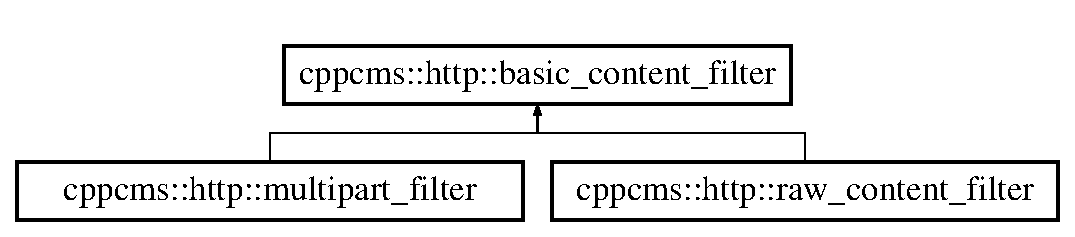
\includegraphics[height=2.000000cm]{classcppcms_1_1http_1_1basic__content__filter}
\end{center}
\end{figure}
\subsection*{Public Member Functions}
\begin{DoxyCompactItemize}
\item 
virtual void {\bf on\+\_\+end\+\_\+of\+\_\+content} ()
\item 
virtual void {\bf on\+\_\+error} ()
\end{DoxyCompactItemize}


\subsection{Detailed Description}
Basic content filter that can be installed to request, all filters should be derived from this base class

Note that when {\ttfamily on\+\_\+$\ast$} member functions of the \doxyref{basic\+\_\+content\+\_\+filter}{p.}{classcppcms_1_1http_1_1basic__content__filter} are called the original application that runs the filtering has temporary installed context that can be accessed from it.

\doxyref{New in Cpp\+C\+MS 1.\+2}{p.}{v1_2} 

\subsection{Member Function Documentation}
\index{cppcms\+::http\+::basic\+\_\+content\+\_\+filter@{cppcms\+::http\+::basic\+\_\+content\+\_\+filter}!on\+\_\+end\+\_\+of\+\_\+content@{on\+\_\+end\+\_\+of\+\_\+content}}
\index{on\+\_\+end\+\_\+of\+\_\+content@{on\+\_\+end\+\_\+of\+\_\+content}!cppcms\+::http\+::basic\+\_\+content\+\_\+filter@{cppcms\+::http\+::basic\+\_\+content\+\_\+filter}}
\subsubsection[{on\+\_\+end\+\_\+of\+\_\+content()}]{\setlength{\rightskip}{0pt plus 5cm}virtual void cppcms\+::http\+::basic\+\_\+content\+\_\+filter\+::on\+\_\+end\+\_\+of\+\_\+content (
\begin{DoxyParamCaption}
{}
\end{DoxyParamCaption}
)\hspace{0.3cm}{\ttfamily [virtual]}}\label{classcppcms_1_1http_1_1basic__content__filter_a77c3fbea0db525449b2d72569b21914a}
Member function that is called when entire content is read. By default does nothing.

The request can be aborted by throwing \doxyref{abort\+\_\+upload}{p.}{classcppcms_1_1http_1_1abort__upload} \index{cppcms\+::http\+::basic\+\_\+content\+\_\+filter@{cppcms\+::http\+::basic\+\_\+content\+\_\+filter}!on\+\_\+error@{on\+\_\+error}}
\index{on\+\_\+error@{on\+\_\+error}!cppcms\+::http\+::basic\+\_\+content\+\_\+filter@{cppcms\+::http\+::basic\+\_\+content\+\_\+filter}}
\subsubsection[{on\+\_\+error()}]{\setlength{\rightskip}{0pt plus 5cm}virtual void cppcms\+::http\+::basic\+\_\+content\+\_\+filter\+::on\+\_\+error (
\begin{DoxyParamCaption}
{}
\end{DoxyParamCaption}
)\hspace{0.3cm}{\ttfamily [virtual]}}\label{classcppcms_1_1http_1_1basic__content__filter_a102acda0950e880fe3dc04ae8616b205}
Member function that is called in case of a error occuring during upload progress, user should not throw exception from this function but rather perform cleanup procedures if needed 

The documentation for this class was generated from the following file\+:\begin{DoxyCompactItemize}
\item 
cppcms/http\+\_\+content\+\_\+filter.\+h\end{DoxyCompactItemize}

\section{booster\+:\+:nowide\+:\+:basic\+\_\+filebuf$<$ Char\+Type, Traits $>$ Class Template Reference}
\label{classbooster_1_1nowide_1_1basic__filebuf}\index{booster\+::nowide\+::basic\+\_\+filebuf$<$ Char\+Type, Traits $>$@{booster\+::nowide\+::basic\+\_\+filebuf$<$ Char\+Type, Traits $>$}}


The documentation for this class was generated from the following file\+:\begin{DoxyCompactItemize}
\item 
booster/nowide/fstream.\+h\end{DoxyCompactItemize}

\section{booster\+:\+:nowide\+:\+:basic\+\_\+filebuf$<$ char $>$ Class Template Reference}
\label{classbooster_1_1nowide_1_1basic__filebuf_3_01char_01_4}\index{booster\+::nowide\+::basic\+\_\+filebuf$<$ char $>$@{booster\+::nowide\+::basic\+\_\+filebuf$<$ char $>$}}


{\ttfamily \#include $<$booster/booster/nowide/fstream.\+h$>$}

Inheritance diagram for booster\+:\+:nowide\+:\+:basic\+\_\+filebuf$<$ char $>$\+:\begin{figure}[H]
\begin{center}
\leavevmode
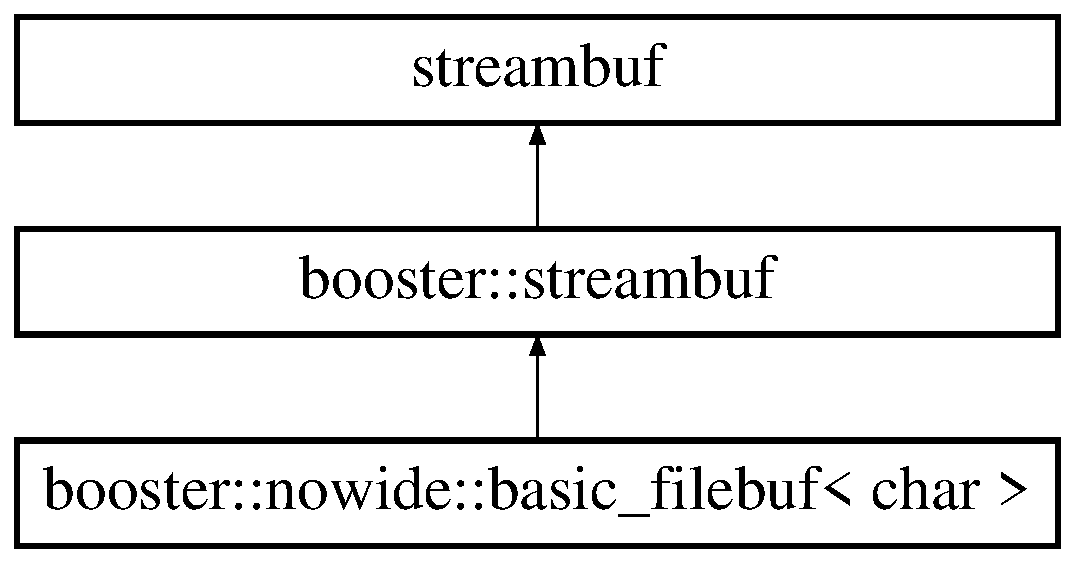
\includegraphics[height=3.000000cm]{classbooster_1_1nowide_1_1basic__filebuf_3_01char_01_4}
\end{center}
\end{figure}
\subsection*{Public Member Functions}
\begin{DoxyCompactItemize}
\item 
{\bf basic\+\_\+filebuf} $\ast$ {\bfseries open} (char const $\ast$s, std\+::ios\+\_\+base\+::openmode mode)\label{classbooster_1_1nowide_1_1basic__filebuf_3_01char_01_4_af53fd41ad94523460647b3a95411a548}

\item 
{\bf basic\+\_\+filebuf} $\ast$ {\bfseries close} ()\label{classbooster_1_1nowide_1_1basic__filebuf_3_01char_01_4_aae0ace743846530c663c267010470126}

\item 
bool {\bfseries is\+\_\+open} () const \label{classbooster_1_1nowide_1_1basic__filebuf_3_01char_01_4_a8c0ba603f3592a54d624e0d91bfab624}

\end{DoxyCompactItemize}
\subsection*{Additional Inherited Members}


\subsection{Detailed Description}
\subsubsection*{template$<$$>$\\*
class booster\+::nowide\+::basic\+\_\+filebuf$<$ char $>$}

Same as std\+::basic\+\_\+filebuf$<$char$>$ but accepts U\+T\+F-\/8 strings under Windows 

The documentation for this class was generated from the following file\+:\begin{DoxyCompactItemize}
\item 
booster/nowide/fstream.\+h\end{DoxyCompactItemize}

\section{booster\+:\+:locale\+:\+:basic\+\_\+format$<$ Char\+Type $>$ Class Template Reference}
\label{classbooster_1_1locale_1_1basic__format}\index{booster\+::locale\+::basic\+\_\+format$<$ Char\+Type $>$@{booster\+::locale\+::basic\+\_\+format$<$ Char\+Type $>$}}


a printf like class that allows type-\/safe and locale aware message formatting  




{\ttfamily \#include $<$booster/booster/locale/format.\+h$>$}

\subsection*{Public Types}
\begin{DoxyCompactItemize}
\item 
typedef Char\+Type {\bf char\+\_\+type}\label{classbooster_1_1locale_1_1basic__format_aede1e07e1af98a6cf4edea1c2ed8cd89}

\begin{DoxyCompactList}\small\item\em Underlying character type. \end{DoxyCompactList}\item 
typedef {\bf basic\+\_\+message}$<$ {\bf char\+\_\+type} $>$ {\bf message\+\_\+type}
\item 
typedef std\+::basic\+\_\+string$<$ Char\+Type $>$ {\bf string\+\_\+type}\label{classbooster_1_1locale_1_1basic__format_a591c3a0ed5134105230987e4f6017a18}

\begin{DoxyCompactList}\small\item\em string type for this type of character \end{DoxyCompactList}\item 
typedef std\+::basic\+\_\+ostream$<$ Char\+Type $>$ {\bf stream\+\_\+type}\label{classbooster_1_1locale_1_1basic__format_aa73e07b4d2ff3f3bc36ceb8ab1a5794b}

\begin{DoxyCompactList}\small\item\em output stream type for this type of character \end{DoxyCompactList}\end{DoxyCompactItemize}
\subsection*{Public Member Functions}
\begin{DoxyCompactItemize}
\item 
{\bf basic\+\_\+format} ({\bf string\+\_\+type} format\+\_\+string)
\item 
{\bf basic\+\_\+format} ({\bf message\+\_\+type} const \&trans)
\item 
{\footnotesize template$<$typename Formattible $>$ }\\{\bf basic\+\_\+format} \& {\bf operator\%} (Formattible const \&object)
\item 
{\bf string\+\_\+type} {\bf str} (std\+::locale const \&loc=std\+::locale()) const 
\item 
void {\bf write} ({\bf stream\+\_\+type} \&out) const 
\end{DoxyCompactItemize}


\subsection{Detailed Description}
\subsubsection*{template$<$typename Char\+Type$>$\\*
class booster\+::locale\+::basic\+\_\+format$<$ Char\+Type $>$}

a printf like class that allows type-\/safe and locale aware message formatting 

This class creates a formatted message similar to printf or boost\+::format and receives formatted entries via operator \%.

For example 
\begin{DoxyCode}
cout << format(\textcolor{stringliteral}{"Hello \{1\}, you are \{2\} years old"}) % name % age << endl;
\end{DoxyCode}


Formatting is enclosed between curly brackets {\ttfamily \{} {\ttfamily \}} and defined by a comma separated list of flags in the format key[=value] value may also be text included between single quotes {\ttfamily \textquotesingle{}} that is used for special purposes where inclusion of non-\/\+A\+S\+C\+II text is allowed

Including of literal {\ttfamily \{} and {\ttfamily \}} is possible by specifying double brackets {\ttfamily \{\{} and {\ttfamily \}\}} accordingly.

For example\+:


\begin{DoxyCode}
cout << format(\textcolor{stringliteral}{"The height of water at \{1,time\} is \{2,num=fixed,precision=3\}"}) % 
      time % height;
\end{DoxyCode}


The special key -- a number without a value defines the position of an input parameter. List of keys\+:
\begin{DoxyItemize}
\item {\ttfamily }[0-\/9]+ -- digits, the index of a formatted parameter -- mandatory key.
\item {\ttfamily num} or {\ttfamily number} -- format a number. Optional values are\+:
\begin{DoxyItemize}
\item {\ttfamily hex} -- display hexadecimal number
\item {\ttfamily oct} -- display in octal format
\item {\ttfamily sci} or {\ttfamily scientific} -- display in scientific format
\item {\ttfamily fix} or {\ttfamily fixed} -- display in fixed format
\end{DoxyItemize}For example {\ttfamily number=sci} 
\item {\ttfamily cur} or {\ttfamily currency} -- format currency. Optional values are\+:
\begin{DoxyItemize}
\item {\ttfamily iso} -- display using I\+SO currency symbol.
\item {\ttfamily nat} or {\ttfamily national} -- display using national currency symbol.
\end{DoxyItemize}
\item {\ttfamily per} or {\ttfamily percent} -- format percent value.
\item {\ttfamily date}, {\ttfamily time} , {\ttfamily datetime} or {\ttfamily dt} -- format date, time or date and time. Optional values are\+:
\begin{DoxyItemize}
\item {\ttfamily s} or {\ttfamily short} -- display in short format
\item {\ttfamily m} or {\ttfamily medium} -- display in medium format.
\item {\ttfamily l} or {\ttfamily long} -- display in long format.
\item {\ttfamily f} or {\ttfamily full} -- display in full format.
\end{DoxyItemize}
\item {\ttfamily ftime} with string (quoted) parameter -- display as with {\ttfamily strftime} see, {\ttfamily \doxyref{as\+::ftime}{p.}{group__manipulators_ga3b395c47f31b0354a0ddb09fcf4ed96f}} manipulator
\item {\ttfamily spell} or {\ttfamily spellout} -- spell the number.
\item {\ttfamily ord} or {\ttfamily ordinal} -- format ordinal number (1st, 2nd... etc)
\item {\ttfamily left} or {\ttfamily $<$} -- align to left.
\item {\ttfamily right} or {\ttfamily $>$} -- align to right.
\item {\ttfamily width} or {\ttfamily w} -- set field width (requires parameter).
\item {\ttfamily precision} or {\ttfamily p} -- set precision (requires parameter).
\item {\ttfamily locale} -- with parameter -- switch locale for current operation. This command generates locale with formatting facets giving more fine grained control of formatting. For example\+: 
\begin{DoxyCode}
cout << format(\textcolor{stringliteral}{"Today \{1,date\} (\{1,date,locale=he\_IL.UTF-8@calendar=hebrew,date\} Hebrew Date)"}) % 
      date;
\end{DoxyCode}

\item {\ttfamily timezone} or {\ttfamily tz} -- the name of the timezone to display the time in. For example\+:~\newline

\begin{DoxyCode}
cout << format(\textcolor{stringliteral}{"Time is: Local \{1,time\}, (\{1,time,tz=EET\} Eastern European Time)"}) % 
      date;
\end{DoxyCode}

\item {\ttfamily local} -\/ display the time in local time
\item {\ttfamily gmt} -\/ display the time in U\+TC time scale 
\begin{DoxyCode}
cout << format(\textcolor{stringliteral}{"Local time is: \{1,time,local\}, universal time is \{1,time,gmt\}"}) % 
      time;
\end{DoxyCode}

\end{DoxyItemize}

Invalid formatting strings are slightly ignored. This would prevent from translator to crash the program in unexpected location. 

\subsection{Member Typedef Documentation}
\index{booster\+::locale\+::basic\+\_\+format@{booster\+::locale\+::basic\+\_\+format}!message\+\_\+type@{message\+\_\+type}}
\index{message\+\_\+type@{message\+\_\+type}!booster\+::locale\+::basic\+\_\+format@{booster\+::locale\+::basic\+\_\+format}}
\subsubsection[{message\+\_\+type}]{\setlength{\rightskip}{0pt plus 5cm}template$<$typename Char\+Type $>$ typedef {\bf basic\+\_\+message}$<${\bf char\+\_\+type}$>$ {\bf booster\+::locale\+::basic\+\_\+format}$<$ Char\+Type $>$\+::{\bf message\+\_\+type}}\label{classbooster_1_1locale_1_1basic__format_a2d21b82a34b4d0e95dac16ce310053ce}
The translation message type 

\subsection{Constructor \& Destructor Documentation}
\index{booster\+::locale\+::basic\+\_\+format@{booster\+::locale\+::basic\+\_\+format}!basic\+\_\+format@{basic\+\_\+format}}
\index{basic\+\_\+format@{basic\+\_\+format}!booster\+::locale\+::basic\+\_\+format@{booster\+::locale\+::basic\+\_\+format}}
\subsubsection[{basic\+\_\+format(string\+\_\+type format\+\_\+string)}]{\setlength{\rightskip}{0pt plus 5cm}template$<$typename Char\+Type $>$ {\bf booster\+::locale\+::basic\+\_\+format}$<$ Char\+Type $>$\+::{\bf basic\+\_\+format} (
\begin{DoxyParamCaption}
\item[{{\bf string\+\_\+type}}]{format\+\_\+string}
\end{DoxyParamCaption}
)\hspace{0.3cm}{\ttfamily [inline]}}\label{classbooster_1_1locale_1_1basic__format_a9a703676d3f99dace1f7b16af406d4f9}
Create a format class for {\itshape format\+\_\+string} \index{booster\+::locale\+::basic\+\_\+format@{booster\+::locale\+::basic\+\_\+format}!basic\+\_\+format@{basic\+\_\+format}}
\index{basic\+\_\+format@{basic\+\_\+format}!booster\+::locale\+::basic\+\_\+format@{booster\+::locale\+::basic\+\_\+format}}
\subsubsection[{basic\+\_\+format(message\+\_\+type const \&trans)}]{\setlength{\rightskip}{0pt plus 5cm}template$<$typename Char\+Type $>$ {\bf booster\+::locale\+::basic\+\_\+format}$<$ Char\+Type $>$\+::{\bf basic\+\_\+format} (
\begin{DoxyParamCaption}
\item[{{\bf message\+\_\+type} const \&}]{trans}
\end{DoxyParamCaption}
)\hspace{0.3cm}{\ttfamily [inline]}}\label{classbooster_1_1locale_1_1basic__format_ac21c8eff853ce4f3da44d1742311f23b}
Create a format class using message {\itshape trans}. The message if translated first according to the rules of target locale and then interpreted as format string 

\subsection{Member Function Documentation}
\index{booster\+::locale\+::basic\+\_\+format@{booster\+::locale\+::basic\+\_\+format}!operator\%@{operator\%}}
\index{operator\%@{operator\%}!booster\+::locale\+::basic\+\_\+format@{booster\+::locale\+::basic\+\_\+format}}
\subsubsection[{operator\%(\+Formattible const \&object)}]{\setlength{\rightskip}{0pt plus 5cm}template$<$typename Char\+Type $>$ template$<$typename Formattible $>$ {\bf basic\+\_\+format}\& {\bf booster\+::locale\+::basic\+\_\+format}$<$ Char\+Type $>$\+::operator\% (
\begin{DoxyParamCaption}
\item[{Formattible const \&}]{object}
\end{DoxyParamCaption}
)\hspace{0.3cm}{\ttfamily [inline]}}\label{classbooster_1_1locale_1_1basic__format_a2fb9cfa5b07ccc47b3b285cd3d8c2b44}
Add new parameter to format list. The object should be a type with defined expression out $<$$<$ object where {\ttfamily out} is {\ttfamily std\+::basic\+\_\+ostream}. \index{booster\+::locale\+::basic\+\_\+format@{booster\+::locale\+::basic\+\_\+format}!str@{str}}
\index{str@{str}!booster\+::locale\+::basic\+\_\+format@{booster\+::locale\+::basic\+\_\+format}}
\subsubsection[{str(std\+::locale const \&loc=std\+::locale()) const }]{\setlength{\rightskip}{0pt plus 5cm}template$<$typename Char\+Type $>$ {\bf string\+\_\+type} {\bf booster\+::locale\+::basic\+\_\+format}$<$ Char\+Type $>$\+::str (
\begin{DoxyParamCaption}
\item[{std\+::locale const \&}]{loc = {\ttfamily std\+:\+:locale()}}
\end{DoxyParamCaption}
) const\hspace{0.3cm}{\ttfamily [inline]}}\label{classbooster_1_1locale_1_1basic__format_a9f9dc98c186e001079bc73e805db7054}
Format a string using a locale {\itshape loc} \index{booster\+::locale\+::basic\+\_\+format@{booster\+::locale\+::basic\+\_\+format}!write@{write}}
\index{write@{write}!booster\+::locale\+::basic\+\_\+format@{booster\+::locale\+::basic\+\_\+format}}
\subsubsection[{write(stream\+\_\+type \&out) const }]{\setlength{\rightskip}{0pt plus 5cm}template$<$typename Char\+Type $>$ void {\bf booster\+::locale\+::basic\+\_\+format}$<$ Char\+Type $>$\+::write (
\begin{DoxyParamCaption}
\item[{{\bf stream\+\_\+type} \&}]{out}
\end{DoxyParamCaption}
) const\hspace{0.3cm}{\ttfamily [inline]}}\label{classbooster_1_1locale_1_1basic__format_a96a673722f6b51dc5068edf18e435a3b}
write a formatted string to output stream {\itshape out} using out\textquotesingle{}s locale 

References booster\+::locale\+::ios\+\_\+info\+::domain\+\_\+id(), and booster\+::locale\+::ios\+\_\+info\+::get().



Referenced by booster\+::locale\+::operator$<$$<$().



The documentation for this class was generated from the following file\+:\begin{DoxyCompactItemize}
\item 
booster/locale/format.\+h\end{DoxyCompactItemize}

\section{booster\+:\+:nowide\+:\+:basic\+\_\+fstream$<$ Char\+Type, Traits $>$ Class Template Reference}
\label{classbooster_1_1nowide_1_1basic__fstream}\index{booster\+::nowide\+::basic\+\_\+fstream$<$ Char\+Type, Traits $>$@{booster\+::nowide\+::basic\+\_\+fstream$<$ Char\+Type, Traits $>$}}


{\ttfamily \#include $<$booster/booster/nowide/fstream.\+h$>$}

Inheritance diagram for booster\+:\+:nowide\+:\+:basic\+\_\+fstream$<$ Char\+Type, Traits $>$\+:\begin{figure}[H]
\begin{center}
\leavevmode
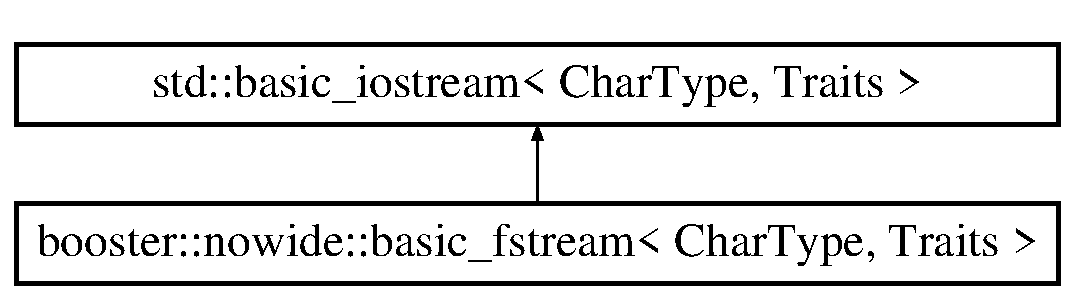
\includegraphics[height=2.000000cm]{classbooster_1_1nowide_1_1basic__fstream}
\end{center}
\end{figure}
\subsection*{Public Types}
\begin{DoxyCompactItemize}
\item 
typedef {\bf basic\+\_\+filebuf}$<$ Char\+Type, Traits $>$ {\bfseries internal\+\_\+buffer\+\_\+type}\label{classbooster_1_1nowide_1_1basic__fstream_a34fd09bc911e53133f4d38e251d6c6e7}

\item 
typedef std\+::basic\+\_\+iostream$<$ Char\+Type, Traits $>$ {\bfseries internal\+\_\+stream\+\_\+type}\label{classbooster_1_1nowide_1_1basic__fstream_a7644af06e695c66947a515214ae17820}

\end{DoxyCompactItemize}
\subsection*{Public Member Functions}
\begin{DoxyCompactItemize}
\item 
{\bfseries basic\+\_\+fstream} (char const $\ast$file\+\_\+name, std\+::ios\+\_\+base\+::openmode mode=std\+::ios\+\_\+base\+::out$\vert$std\+::ios\+\_\+base\+::in)\label{classbooster_1_1nowide_1_1basic__fstream_a19bf2f035f508e8912dd7ca2226aa3ac}

\item 
void {\bfseries open} (char const $\ast$file\+\_\+name, std\+::ios\+\_\+base\+::openmode mode=std\+::ios\+\_\+base\+::out$\vert$std\+::ios\+\_\+base\+::out)\label{classbooster_1_1nowide_1_1basic__fstream_a8bd6973e1d307904b913838db1601fe1}

\item 
bool {\bfseries is\+\_\+open} ()\label{classbooster_1_1nowide_1_1basic__fstream_aa935f6d90db9050d7d7d41ff92600495}

\item 
bool {\bfseries is\+\_\+open} () const \label{classbooster_1_1nowide_1_1basic__fstream_a51b8ed3cbf427146d8396c70a68726e8}

\item 
void {\bfseries close} ()\label{classbooster_1_1nowide_1_1basic__fstream_ad07239315e831d3be0d6468e6e1d964a}

\item 
{\bf internal\+\_\+buffer\+\_\+type} $\ast$ {\bfseries rdbuf} () const \label{classbooster_1_1nowide_1_1basic__fstream_ac60c9e9e38d4fbd030c30be89b5a1b62}

\end{DoxyCompactItemize}


\subsection{Detailed Description}
\subsubsection*{template$<$typename Char\+Type, typename Traits = std\+::char\+\_\+traits$<$\+Char\+Type$>$$>$\\*
class booster\+::nowide\+::basic\+\_\+fstream$<$ Char\+Type, Traits $>$}

Same as std\+::basic\+\_\+fstream$<$char$>$ but accepts U\+T\+F-\/8 strings under Windows 

The documentation for this class was generated from the following file\+:\begin{DoxyCompactItemize}
\item 
booster/nowide/fstream.\+h\end{DoxyCompactItemize}

\section{booster\+:\+:nowide\+:\+:basic\+\_\+ifstream$<$ Char\+Type, Traits $>$ Class Template Reference}
\label{classbooster_1_1nowide_1_1basic__ifstream}\index{booster\+::nowide\+::basic\+\_\+ifstream$<$ Char\+Type, Traits $>$@{booster\+::nowide\+::basic\+\_\+ifstream$<$ Char\+Type, Traits $>$}}


{\ttfamily \#include $<$booster/booster/nowide/fstream.\+h$>$}

Inheritance diagram for booster\+:\+:nowide\+:\+:basic\+\_\+ifstream$<$ Char\+Type, Traits $>$\+:\begin{figure}[H]
\begin{center}
\leavevmode
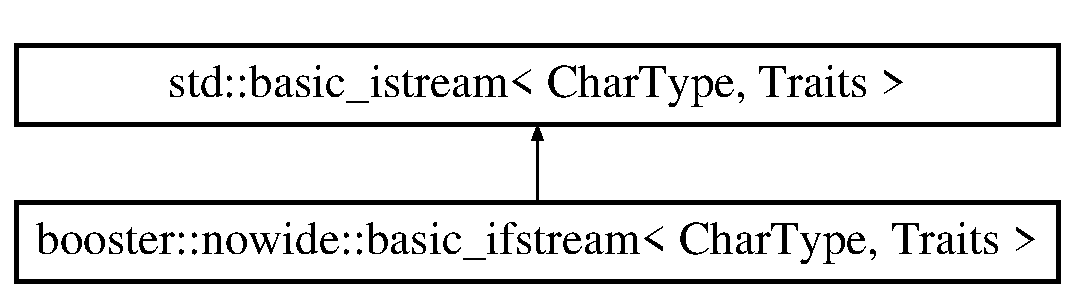
\includegraphics[height=2.000000cm]{classbooster_1_1nowide_1_1basic__ifstream}
\end{center}
\end{figure}
\subsection*{Public Types}
\begin{DoxyCompactItemize}
\item 
typedef {\bf basic\+\_\+filebuf}$<$ Char\+Type, Traits $>$ {\bfseries internal\+\_\+buffer\+\_\+type}\label{classbooster_1_1nowide_1_1basic__ifstream_a69bfa84177d7a4d357958164a2015b3c}

\item 
typedef std\+::basic\+\_\+istream$<$ Char\+Type, Traits $>$ {\bfseries internal\+\_\+stream\+\_\+type}\label{classbooster_1_1nowide_1_1basic__ifstream_a9baee407ad1c3fd5ac837b206ed122c8}

\end{DoxyCompactItemize}
\subsection*{Public Member Functions}
\begin{DoxyCompactItemize}
\item 
{\bfseries basic\+\_\+ifstream} (char const $\ast$file\+\_\+name, std\+::ios\+\_\+base\+::openmode mode=std\+::ios\+\_\+base\+::in)\label{classbooster_1_1nowide_1_1basic__ifstream_a349a1df7d87c85422e67574d8d0f17ab}

\item 
void {\bfseries open} (char const $\ast$file\+\_\+name, std\+::ios\+\_\+base\+::openmode mode=std\+::ios\+\_\+base\+::in)\label{classbooster_1_1nowide_1_1basic__ifstream_a09b6a2cb66805759abd7c130e18b5896}

\item 
bool {\bfseries is\+\_\+open} ()\label{classbooster_1_1nowide_1_1basic__ifstream_a5ab0ecf734809cf43f3753783e797357}

\item 
bool {\bfseries is\+\_\+open} () const \label{classbooster_1_1nowide_1_1basic__ifstream_aaba31ae640976c974c60f1e560379007}

\item 
void {\bfseries close} ()\label{classbooster_1_1nowide_1_1basic__ifstream_af39fe9e62c854ea5ba2333d469a6cf79}

\item 
{\bf internal\+\_\+buffer\+\_\+type} $\ast$ {\bfseries rdbuf} () const \label{classbooster_1_1nowide_1_1basic__ifstream_a1ac8e4f67a2f66b6be0ac15a20c078ae}

\end{DoxyCompactItemize}


\subsection{Detailed Description}
\subsubsection*{template$<$typename Char\+Type, typename Traits = std\+::char\+\_\+traits$<$\+Char\+Type$>$$>$\\*
class booster\+::nowide\+::basic\+\_\+ifstream$<$ Char\+Type, Traits $>$}

Same as std\+::basic\+\_\+ifstream$<$char$>$ but accepts U\+T\+F-\/8 strings under Windows 

The documentation for this class was generated from the following file\+:\begin{DoxyCompactItemize}
\item 
booster/nowide/fstream.\+h\end{DoxyCompactItemize}

\section{booster\+:\+:aio\+:\+:basic\+\_\+io\+\_\+device Class Reference}
\label{classbooster_1_1aio_1_1basic__io__device}\index{booster\+::aio\+::basic\+\_\+io\+\_\+device@{booster\+::aio\+::basic\+\_\+io\+\_\+device}}


This is a basic object that allows execution of asynchronous operations.  




{\ttfamily \#include $<$booster/booster/aio/basic\+\_\+io\+\_\+device.\+h$>$}

Inheritance diagram for booster\+:\+:aio\+:\+:basic\+\_\+io\+\_\+device\+:\begin{figure}[H]
\begin{center}
\leavevmode
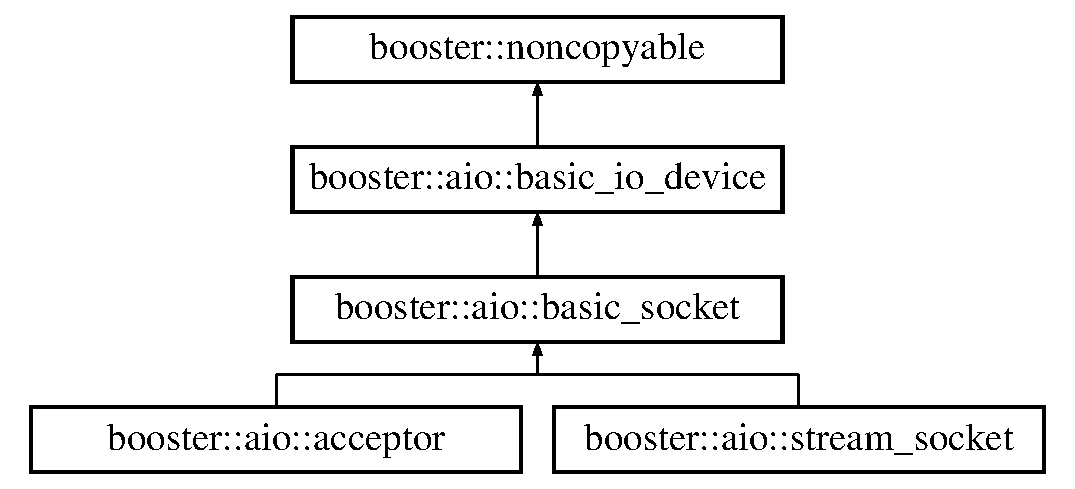
\includegraphics[height=4.000000cm]{classbooster_1_1aio_1_1basic__io__device}
\end{center}
\end{figure}
\subsection*{Public Member Functions}
\begin{DoxyCompactItemize}
\item 
{\bf basic\+\_\+io\+\_\+device} ()
\item 
{\bf basic\+\_\+io\+\_\+device} ({\bf io\+\_\+service} \&srv)
\item 
virtual {\bf $\sim$basic\+\_\+io\+\_\+device} ()
\item 
bool {\bf has\+\_\+io\+\_\+service} ()
\item 
{\bf io\+\_\+service} \& {\bf get\+\_\+io\+\_\+service} ()
\item 
void {\bf set\+\_\+io\+\_\+service} ({\bf io\+\_\+service} \&srv)
\item 
void {\bf reset\+\_\+io\+\_\+service} ()
\item 
void {\bf attach} ({\bf native\+\_\+type} fd)
\item 
void {\bf assign} ({\bf native\+\_\+type} fd)
\item 
{\bf native\+\_\+type} {\bf release} ()
\item 
{\bf native\+\_\+type} {\bf native} ()
\item 
void {\bf close} ()
\item 
void {\bf close} (system\+::error\+\_\+code \&e)
\item 
void {\bf on\+\_\+readable} ({\bf event\+\_\+handler} const \&r)
\item 
void {\bf on\+\_\+writeable} ({\bf event\+\_\+handler} const \&r)
\item 
void {\bf cancel} ()
\item 
{\bf basic\+\_\+io\+\_\+device} \& {\bf lowest\+\_\+layer} ()
\item 
void {\bf set\+\_\+non\+\_\+blocking} (bool nonblocking)
\item 
void {\bf set\+\_\+non\+\_\+blocking} (bool nonblocking, system\+::error\+\_\+code \&e)
\item 
void {\bf set\+\_\+non\+\_\+blocking\+\_\+if\+\_\+needed} (bool nonblocking)
\item 
void {\bf set\+\_\+non\+\_\+blocking\+\_\+if\+\_\+needed} (bool nonblocking, system\+::error\+\_\+code \&e)
\end{DoxyCompactItemize}
\subsection*{Static Public Member Functions}
\begin{DoxyCompactItemize}
\item 
static bool {\bf would\+\_\+block} (system\+::error\+\_\+code const \&e)
\end{DoxyCompactItemize}
\subsection*{Protected Member Functions}
\begin{DoxyCompactItemize}
\item 
bool {\bf dont\+\_\+block} ({\bf event\+\_\+handler} const \&c)
\item 
bool {\bf dont\+\_\+block} ({\bf io\+\_\+handler} const \&c)
\end{DoxyCompactItemize}


\subsection{Detailed Description}
This is a basic object that allows execution of asynchronous operations. 

It represents a generic \char`\"{}select\char`\"{}able file descriptor or S\+O\+C\+K\+ET on Windows platform.

It does following\+:


\begin{DoxyItemize}
\item Connects an object with the event loop -\/ \doxyref{io\+\_\+service}{p.}{classbooster_1_1aio_1_1io__service}
\item Allows to connect and disconnect native file descriptor/socket object to it, and close it
\item Asynchronously poll the object for readability and writeability via \doxyref{io\+\_\+service}{p.}{classbooster_1_1aio_1_1io__service} object and cancel such operations
\item Switch blocking and non-\/blocking mode of the descriptor. 
\end{DoxyItemize}

\subsection{Constructor \& Destructor Documentation}
\index{booster\+::aio\+::basic\+\_\+io\+\_\+device@{booster\+::aio\+::basic\+\_\+io\+\_\+device}!basic\+\_\+io\+\_\+device@{basic\+\_\+io\+\_\+device}}
\index{basic\+\_\+io\+\_\+device@{basic\+\_\+io\+\_\+device}!booster\+::aio\+::basic\+\_\+io\+\_\+device@{booster\+::aio\+::basic\+\_\+io\+\_\+device}}
\subsubsection[{basic\+\_\+io\+\_\+device()}]{\setlength{\rightskip}{0pt plus 5cm}booster\+::aio\+::basic\+\_\+io\+\_\+device\+::basic\+\_\+io\+\_\+device (
\begin{DoxyParamCaption}
{}
\end{DoxyParamCaption}
)}\label{classbooster_1_1aio_1_1basic__io__device_a6635e83332c8e5446846360bfe73ffa4}
Create a new device not attached to event loop \index{booster\+::aio\+::basic\+\_\+io\+\_\+device@{booster\+::aio\+::basic\+\_\+io\+\_\+device}!basic\+\_\+io\+\_\+device@{basic\+\_\+io\+\_\+device}}
\index{basic\+\_\+io\+\_\+device@{basic\+\_\+io\+\_\+device}!booster\+::aio\+::basic\+\_\+io\+\_\+device@{booster\+::aio\+::basic\+\_\+io\+\_\+device}}
\subsubsection[{basic\+\_\+io\+\_\+device(io\+\_\+service \&srv)}]{\setlength{\rightskip}{0pt plus 5cm}booster\+::aio\+::basic\+\_\+io\+\_\+device\+::basic\+\_\+io\+\_\+device (
\begin{DoxyParamCaption}
\item[{{\bf io\+\_\+service} \&}]{srv}
\end{DoxyParamCaption}
)}\label{classbooster_1_1aio_1_1basic__io__device_a0b8f8ffb18b05ec054ae30400e8ad11b}
Create a new device that is attached to the event loop {\itshape srv} \index{booster\+::aio\+::basic\+\_\+io\+\_\+device@{booster\+::aio\+::basic\+\_\+io\+\_\+device}!````~basic\+\_\+io\+\_\+device@{$\sim$basic\+\_\+io\+\_\+device}}
\index{````~basic\+\_\+io\+\_\+device@{$\sim$basic\+\_\+io\+\_\+device}!booster\+::aio\+::basic\+\_\+io\+\_\+device@{booster\+::aio\+::basic\+\_\+io\+\_\+device}}
\subsubsection[{$\sim$basic\+\_\+io\+\_\+device()}]{\setlength{\rightskip}{0pt plus 5cm}virtual booster\+::aio\+::basic\+\_\+io\+\_\+device\+::$\sim$basic\+\_\+io\+\_\+device (
\begin{DoxyParamCaption}
{}
\end{DoxyParamCaption}
)\hspace{0.3cm}{\ttfamily [virtual]}}\label{classbooster_1_1aio_1_1basic__io__device_a35bd2108e6654eb12b9996992ff278bb}
Destroy the object. If it owns the file descriptor or socket it closes it 

\subsection{Member Function Documentation}
\index{booster\+::aio\+::basic\+\_\+io\+\_\+device@{booster\+::aio\+::basic\+\_\+io\+\_\+device}!assign@{assign}}
\index{assign@{assign}!booster\+::aio\+::basic\+\_\+io\+\_\+device@{booster\+::aio\+::basic\+\_\+io\+\_\+device}}
\subsubsection[{assign(native\+\_\+type fd)}]{\setlength{\rightskip}{0pt plus 5cm}void booster\+::aio\+::basic\+\_\+io\+\_\+device\+::assign (
\begin{DoxyParamCaption}
\item[{{\bf native\+\_\+type}}]{fd}
\end{DoxyParamCaption}
)}\label{classbooster_1_1aio_1_1basic__io__device_afba3662e557aa44834257ffc063e0cb1}
Assign existing file descriptor {\itshape fd} to the device. The ownership is transferred to the object \index{booster\+::aio\+::basic\+\_\+io\+\_\+device@{booster\+::aio\+::basic\+\_\+io\+\_\+device}!attach@{attach}}
\index{attach@{attach}!booster\+::aio\+::basic\+\_\+io\+\_\+device@{booster\+::aio\+::basic\+\_\+io\+\_\+device}}
\subsubsection[{attach(native\+\_\+type fd)}]{\setlength{\rightskip}{0pt plus 5cm}void booster\+::aio\+::basic\+\_\+io\+\_\+device\+::attach (
\begin{DoxyParamCaption}
\item[{{\bf native\+\_\+type}}]{fd}
\end{DoxyParamCaption}
)}\label{classbooster_1_1aio_1_1basic__io__device_ad327ab1cc9323bb8f4c641d0f3eb186a}
Attach the file descriptor {\itshape fd} to the device. The ownership is not transferred to the object.

If \doxyref{basic\+\_\+io\+\_\+device}{p.}{classbooster_1_1aio_1_1basic__io__device} owns other file descriptor, it is closed. \index{booster\+::aio\+::basic\+\_\+io\+\_\+device@{booster\+::aio\+::basic\+\_\+io\+\_\+device}!cancel@{cancel}}
\index{cancel@{cancel}!booster\+::aio\+::basic\+\_\+io\+\_\+device@{booster\+::aio\+::basic\+\_\+io\+\_\+device}}
\subsubsection[{cancel()}]{\setlength{\rightskip}{0pt plus 5cm}void booster\+::aio\+::basic\+\_\+io\+\_\+device\+::cancel (
\begin{DoxyParamCaption}
{}
\end{DoxyParamCaption}
)}\label{classbooster_1_1aio_1_1basic__io__device_a90aee159a796481187a0721ccd6d96b1}
Cancel all asynchronous operations. \index{booster\+::aio\+::basic\+\_\+io\+\_\+device@{booster\+::aio\+::basic\+\_\+io\+\_\+device}!close@{close}}
\index{close@{close}!booster\+::aio\+::basic\+\_\+io\+\_\+device@{booster\+::aio\+::basic\+\_\+io\+\_\+device}}
\subsubsection[{close()}]{\setlength{\rightskip}{0pt plus 5cm}void booster\+::aio\+::basic\+\_\+io\+\_\+device\+::close (
\begin{DoxyParamCaption}
{}
\end{DoxyParamCaption}
)}\label{classbooster_1_1aio_1_1basic__io__device_a8f53c02046939cb90ffdf2f865676e4f}
Cancels all pending asynchronous events. If the ownership belongs to it closes the file descriptor.

Throws system\+::system\+\_\+error if error occurs. \index{booster\+::aio\+::basic\+\_\+io\+\_\+device@{booster\+::aio\+::basic\+\_\+io\+\_\+device}!close@{close}}
\index{close@{close}!booster\+::aio\+::basic\+\_\+io\+\_\+device@{booster\+::aio\+::basic\+\_\+io\+\_\+device}}
\subsubsection[{close(system\+::error\+\_\+code \&e)}]{\setlength{\rightskip}{0pt plus 5cm}void booster\+::aio\+::basic\+\_\+io\+\_\+device\+::close (
\begin{DoxyParamCaption}
\item[{system\+::error\+\_\+code \&}]{e}
\end{DoxyParamCaption}
)}\label{classbooster_1_1aio_1_1basic__io__device_aea32fc85e3cf9a07e80bd7e200bdc441}
Cancels all pending asynchronous events. If the ownership belongs to it closes the file descriptor.

If a error occurs it is assigned to {\itshape e}. \index{booster\+::aio\+::basic\+\_\+io\+\_\+device@{booster\+::aio\+::basic\+\_\+io\+\_\+device}!dont\+\_\+block@{dont\+\_\+block}}
\index{dont\+\_\+block@{dont\+\_\+block}!booster\+::aio\+::basic\+\_\+io\+\_\+device@{booster\+::aio\+::basic\+\_\+io\+\_\+device}}
\subsubsection[{dont\+\_\+block(event\+\_\+handler const \&c)}]{\setlength{\rightskip}{0pt plus 5cm}bool booster\+::aio\+::basic\+\_\+io\+\_\+device\+::dont\+\_\+block (
\begin{DoxyParamCaption}
\item[{{\bf event\+\_\+handler} const \&}]{c}
\end{DoxyParamCaption}
)\hspace{0.3cm}{\ttfamily [protected]}}\label{classbooster_1_1aio_1_1basic__io__device_a15d1ca42e67eb46985ff6cb94b931f49}
Set non-\/blocking mode. If error occurs returns false and the error is reported via callback c \index{booster\+::aio\+::basic\+\_\+io\+\_\+device@{booster\+::aio\+::basic\+\_\+io\+\_\+device}!dont\+\_\+block@{dont\+\_\+block}}
\index{dont\+\_\+block@{dont\+\_\+block}!booster\+::aio\+::basic\+\_\+io\+\_\+device@{booster\+::aio\+::basic\+\_\+io\+\_\+device}}
\subsubsection[{dont\+\_\+block(io\+\_\+handler const \&c)}]{\setlength{\rightskip}{0pt plus 5cm}bool booster\+::aio\+::basic\+\_\+io\+\_\+device\+::dont\+\_\+block (
\begin{DoxyParamCaption}
\item[{{\bf io\+\_\+handler} const \&}]{c}
\end{DoxyParamCaption}
)\hspace{0.3cm}{\ttfamily [protected]}}\label{classbooster_1_1aio_1_1basic__io__device_a3047ab5c9c37b5d533526afe7a455b92}
Set non-\/blocking mode. If error occurs returns false and the error is reported via callback c \index{booster\+::aio\+::basic\+\_\+io\+\_\+device@{booster\+::aio\+::basic\+\_\+io\+\_\+device}!get\+\_\+io\+\_\+service@{get\+\_\+io\+\_\+service}}
\index{get\+\_\+io\+\_\+service@{get\+\_\+io\+\_\+service}!booster\+::aio\+::basic\+\_\+io\+\_\+device@{booster\+::aio\+::basic\+\_\+io\+\_\+device}}
\subsubsection[{get\+\_\+io\+\_\+service()}]{\setlength{\rightskip}{0pt plus 5cm}{\bf io\+\_\+service}\& booster\+::aio\+::basic\+\_\+io\+\_\+device\+::get\+\_\+io\+\_\+service (
\begin{DoxyParamCaption}
{}
\end{DoxyParamCaption}
)}\label{classbooster_1_1aio_1_1basic__io__device_a5213f9255c418b78bdb98d5da96e2a7e}
Returns the connected \doxyref{io\+\_\+service}{p.}{classbooster_1_1aio_1_1io__service}, throws system\+::system\+\_\+error if no \doxyref{io\+\_\+service}{p.}{classbooster_1_1aio_1_1io__service} connected \index{booster\+::aio\+::basic\+\_\+io\+\_\+device@{booster\+::aio\+::basic\+\_\+io\+\_\+device}!has\+\_\+io\+\_\+service@{has\+\_\+io\+\_\+service}}
\index{has\+\_\+io\+\_\+service@{has\+\_\+io\+\_\+service}!booster\+::aio\+::basic\+\_\+io\+\_\+device@{booster\+::aio\+::basic\+\_\+io\+\_\+device}}
\subsubsection[{has\+\_\+io\+\_\+service()}]{\setlength{\rightskip}{0pt plus 5cm}bool booster\+::aio\+::basic\+\_\+io\+\_\+device\+::has\+\_\+io\+\_\+service (
\begin{DoxyParamCaption}
{}
\end{DoxyParamCaption}
)}\label{classbooster_1_1aio_1_1basic__io__device_a74dcacdfa8bdf111723f3e0daa26348d}
Check if the \doxyref{basic\+\_\+io\+\_\+device}{p.}{classbooster_1_1aio_1_1basic__io__device} is connected to the \doxyref{io\+\_\+service}{p.}{classbooster_1_1aio_1_1io__service} \index{booster\+::aio\+::basic\+\_\+io\+\_\+device@{booster\+::aio\+::basic\+\_\+io\+\_\+device}!lowest\+\_\+layer@{lowest\+\_\+layer}}
\index{lowest\+\_\+layer@{lowest\+\_\+layer}!booster\+::aio\+::basic\+\_\+io\+\_\+device@{booster\+::aio\+::basic\+\_\+io\+\_\+device}}
\subsubsection[{lowest\+\_\+layer()}]{\setlength{\rightskip}{0pt plus 5cm}{\bf basic\+\_\+io\+\_\+device}\& booster\+::aio\+::basic\+\_\+io\+\_\+device\+::lowest\+\_\+layer (
\begin{DoxyParamCaption}
{}
\end{DoxyParamCaption}
)}\label{classbooster_1_1aio_1_1basic__io__device_a673dfae98eb87a77aef359026156d21f}
Returns $\ast$this \index{booster\+::aio\+::basic\+\_\+io\+\_\+device@{booster\+::aio\+::basic\+\_\+io\+\_\+device}!native@{native}}
\index{native@{native}!booster\+::aio\+::basic\+\_\+io\+\_\+device@{booster\+::aio\+::basic\+\_\+io\+\_\+device}}
\subsubsection[{native()}]{\setlength{\rightskip}{0pt plus 5cm}{\bf native\+\_\+type} booster\+::aio\+::basic\+\_\+io\+\_\+device\+::native (
\begin{DoxyParamCaption}
{}
\end{DoxyParamCaption}
)}\label{classbooster_1_1aio_1_1basic__io__device_aaec15c09a2a3b3c086797cb6e8fbbd3a}
Get the underlying file descriptor. Returns invalid\+\_\+socket if the file descriptor was not assigned \index{booster\+::aio\+::basic\+\_\+io\+\_\+device@{booster\+::aio\+::basic\+\_\+io\+\_\+device}!on\+\_\+readable@{on\+\_\+readable}}
\index{on\+\_\+readable@{on\+\_\+readable}!booster\+::aio\+::basic\+\_\+io\+\_\+device@{booster\+::aio\+::basic\+\_\+io\+\_\+device}}
\subsubsection[{on\+\_\+readable(event\+\_\+handler const \&r)}]{\setlength{\rightskip}{0pt plus 5cm}void booster\+::aio\+::basic\+\_\+io\+\_\+device\+::on\+\_\+readable (
\begin{DoxyParamCaption}
\item[{{\bf event\+\_\+handler} const \&}]{r}
\end{DoxyParamCaption}
)}\label{classbooster_1_1aio_1_1basic__io__device_a62f19c716b2a83bbb24b0ab81f268b4b}
Start asynchronous polling for readability. The result is reported via callback {\itshape r}.

If \doxyref{io\+\_\+service}{p.}{classbooster_1_1aio_1_1io__service} is not assigned throws system\+::system\+\_\+error, all other errors reported via {\itshape r}. \index{booster\+::aio\+::basic\+\_\+io\+\_\+device@{booster\+::aio\+::basic\+\_\+io\+\_\+device}!on\+\_\+writeable@{on\+\_\+writeable}}
\index{on\+\_\+writeable@{on\+\_\+writeable}!booster\+::aio\+::basic\+\_\+io\+\_\+device@{booster\+::aio\+::basic\+\_\+io\+\_\+device}}
\subsubsection[{on\+\_\+writeable(event\+\_\+handler const \&r)}]{\setlength{\rightskip}{0pt plus 5cm}void booster\+::aio\+::basic\+\_\+io\+\_\+device\+::on\+\_\+writeable (
\begin{DoxyParamCaption}
\item[{{\bf event\+\_\+handler} const \&}]{r}
\end{DoxyParamCaption}
)}\label{classbooster_1_1aio_1_1basic__io__device_a92348b74bcf7d14985a388f16381423b}
Start asynchronous polling for writeability. The result is reported via callback {\itshape r}.

If \doxyref{io\+\_\+service}{p.}{classbooster_1_1aio_1_1io__service} is not assigned throws system\+::system\+\_\+error, all other errors reported via {\itshape r}. \index{booster\+::aio\+::basic\+\_\+io\+\_\+device@{booster\+::aio\+::basic\+\_\+io\+\_\+device}!release@{release}}
\index{release@{release}!booster\+::aio\+::basic\+\_\+io\+\_\+device@{booster\+::aio\+::basic\+\_\+io\+\_\+device}}
\subsubsection[{release()}]{\setlength{\rightskip}{0pt plus 5cm}{\bf native\+\_\+type} booster\+::aio\+::basic\+\_\+io\+\_\+device\+::release (
\begin{DoxyParamCaption}
{}
\end{DoxyParamCaption}
)}\label{classbooster_1_1aio_1_1basic__io__device_aecf495a71b20c55a1e5b68180d531916}
Release the ownership on the current file descriptor. The user is responsible to close it.

\begin{DoxyNote}{Note}
it just changes the \char`\"{}ownership\char`\"{} flag in the object, nothing else is done 
\end{DoxyNote}
\index{booster\+::aio\+::basic\+\_\+io\+\_\+device@{booster\+::aio\+::basic\+\_\+io\+\_\+device}!reset\+\_\+io\+\_\+service@{reset\+\_\+io\+\_\+service}}
\index{reset\+\_\+io\+\_\+service@{reset\+\_\+io\+\_\+service}!booster\+::aio\+::basic\+\_\+io\+\_\+device@{booster\+::aio\+::basic\+\_\+io\+\_\+device}}
\subsubsection[{reset\+\_\+io\+\_\+service()}]{\setlength{\rightskip}{0pt plus 5cm}void booster\+::aio\+::basic\+\_\+io\+\_\+device\+::reset\+\_\+io\+\_\+service (
\begin{DoxyParamCaption}
{}
\end{DoxyParamCaption}
)}\label{classbooster_1_1aio_1_1basic__io__device_af680d21d232d2e1f12f8e2bdc2ab8483}
Detaches the object from \doxyref{io\+\_\+service}{p.}{classbooster_1_1aio_1_1io__service}. Cancels all pending asynchronous operations. \index{booster\+::aio\+::basic\+\_\+io\+\_\+device@{booster\+::aio\+::basic\+\_\+io\+\_\+device}!set\+\_\+io\+\_\+service@{set\+\_\+io\+\_\+service}}
\index{set\+\_\+io\+\_\+service@{set\+\_\+io\+\_\+service}!booster\+::aio\+::basic\+\_\+io\+\_\+device@{booster\+::aio\+::basic\+\_\+io\+\_\+device}}
\subsubsection[{set\+\_\+io\+\_\+service(io\+\_\+service \&srv)}]{\setlength{\rightskip}{0pt plus 5cm}void booster\+::aio\+::basic\+\_\+io\+\_\+device\+::set\+\_\+io\+\_\+service (
\begin{DoxyParamCaption}
\item[{{\bf io\+\_\+service} \&}]{srv}
\end{DoxyParamCaption}
)}\label{classbooster_1_1aio_1_1basic__io__device_acbf4de1f8e1a9d4503d5e2225b0be801}
Sets new \doxyref{io\+\_\+service}{p.}{classbooster_1_1aio_1_1io__service}. Cancels all pending asynchronous operations on the connected \doxyref{io\+\_\+service}{p.}{classbooster_1_1aio_1_1io__service}. \index{booster\+::aio\+::basic\+\_\+io\+\_\+device@{booster\+::aio\+::basic\+\_\+io\+\_\+device}!set\+\_\+non\+\_\+blocking@{set\+\_\+non\+\_\+blocking}}
\index{set\+\_\+non\+\_\+blocking@{set\+\_\+non\+\_\+blocking}!booster\+::aio\+::basic\+\_\+io\+\_\+device@{booster\+::aio\+::basic\+\_\+io\+\_\+device}}
\subsubsection[{set\+\_\+non\+\_\+blocking(bool nonblocking)}]{\setlength{\rightskip}{0pt plus 5cm}void booster\+::aio\+::basic\+\_\+io\+\_\+device\+::set\+\_\+non\+\_\+blocking (
\begin{DoxyParamCaption}
\item[{bool}]{nonblocking}
\end{DoxyParamCaption}
)}\label{classbooster_1_1aio_1_1basic__io__device_a989ff34ab1e49d27a4f72de344605f39}
Set the object to blocking or non-\/blocking mode.

Throws system\+::system\+\_\+error if error occurs. \index{booster\+::aio\+::basic\+\_\+io\+\_\+device@{booster\+::aio\+::basic\+\_\+io\+\_\+device}!set\+\_\+non\+\_\+blocking@{set\+\_\+non\+\_\+blocking}}
\index{set\+\_\+non\+\_\+blocking@{set\+\_\+non\+\_\+blocking}!booster\+::aio\+::basic\+\_\+io\+\_\+device@{booster\+::aio\+::basic\+\_\+io\+\_\+device}}
\subsubsection[{set\+\_\+non\+\_\+blocking(bool nonblocking, system\+::error\+\_\+code \&e)}]{\setlength{\rightskip}{0pt plus 5cm}void booster\+::aio\+::basic\+\_\+io\+\_\+device\+::set\+\_\+non\+\_\+blocking (
\begin{DoxyParamCaption}
\item[{bool}]{nonblocking, }
\item[{system\+::error\+\_\+code \&}]{e}
\end{DoxyParamCaption}
)}\label{classbooster_1_1aio_1_1basic__io__device_ad224749aff0c2a54b46aac8d6b7aa53a}
Set the object to blocking or non-\/blocking mode.

If a error occurs it is assigned to {\itshape e}. \index{booster\+::aio\+::basic\+\_\+io\+\_\+device@{booster\+::aio\+::basic\+\_\+io\+\_\+device}!set\+\_\+non\+\_\+blocking\+\_\+if\+\_\+needed@{set\+\_\+non\+\_\+blocking\+\_\+if\+\_\+needed}}
\index{set\+\_\+non\+\_\+blocking\+\_\+if\+\_\+needed@{set\+\_\+non\+\_\+blocking\+\_\+if\+\_\+needed}!booster\+::aio\+::basic\+\_\+io\+\_\+device@{booster\+::aio\+::basic\+\_\+io\+\_\+device}}
\subsubsection[{set\+\_\+non\+\_\+blocking\+\_\+if\+\_\+needed(bool nonblocking)}]{\setlength{\rightskip}{0pt plus 5cm}void booster\+::aio\+::basic\+\_\+io\+\_\+device\+::set\+\_\+non\+\_\+blocking\+\_\+if\+\_\+needed (
\begin{DoxyParamCaption}
\item[{bool}]{nonblocking}
\end{DoxyParamCaption}
)}\label{classbooster_1_1aio_1_1basic__io__device_a9427190b440f40ebdec3cab8d962b055}
Set the object to blocking or non-\/blocking mode. It checks if \doxyref{set\+\_\+non\+\_\+blocking()}{p.}{classbooster_1_1aio_1_1basic__io__device_a989ff34ab1e49d27a4f72de344605f39} was called before and does nothing if previous call matches the request

Throws system\+::system\+\_\+error if error occurs.

\doxyref{New in Cpp\+C\+MS 1.\+2}{p.}{v1_2} \index{booster\+::aio\+::basic\+\_\+io\+\_\+device@{booster\+::aio\+::basic\+\_\+io\+\_\+device}!set\+\_\+non\+\_\+blocking\+\_\+if\+\_\+needed@{set\+\_\+non\+\_\+blocking\+\_\+if\+\_\+needed}}
\index{set\+\_\+non\+\_\+blocking\+\_\+if\+\_\+needed@{set\+\_\+non\+\_\+blocking\+\_\+if\+\_\+needed}!booster\+::aio\+::basic\+\_\+io\+\_\+device@{booster\+::aio\+::basic\+\_\+io\+\_\+device}}
\subsubsection[{set\+\_\+non\+\_\+blocking\+\_\+if\+\_\+needed(bool nonblocking, system\+::error\+\_\+code \&e)}]{\setlength{\rightskip}{0pt plus 5cm}void booster\+::aio\+::basic\+\_\+io\+\_\+device\+::set\+\_\+non\+\_\+blocking\+\_\+if\+\_\+needed (
\begin{DoxyParamCaption}
\item[{bool}]{nonblocking, }
\item[{system\+::error\+\_\+code \&}]{e}
\end{DoxyParamCaption}
)}\label{classbooster_1_1aio_1_1basic__io__device_a6bad4b9af753fc5cce3a3c241d75e6ed}
Set the object to blocking or non-\/blocking mode. It checks if \doxyref{set\+\_\+non\+\_\+blocking()}{p.}{classbooster_1_1aio_1_1basic__io__device_a989ff34ab1e49d27a4f72de344605f39} was called before and does nothing if previous call matches the request

If a error occurs it is assigned to {\itshape e}.

\doxyref{New in Cpp\+C\+MS 1.\+2}{p.}{v1_2} \index{booster\+::aio\+::basic\+\_\+io\+\_\+device@{booster\+::aio\+::basic\+\_\+io\+\_\+device}!would\+\_\+block@{would\+\_\+block}}
\index{would\+\_\+block@{would\+\_\+block}!booster\+::aio\+::basic\+\_\+io\+\_\+device@{booster\+::aio\+::basic\+\_\+io\+\_\+device}}
\subsubsection[{would\+\_\+block(system\+::error\+\_\+code const \&e)}]{\setlength{\rightskip}{0pt plus 5cm}static bool booster\+::aio\+::basic\+\_\+io\+\_\+device\+::would\+\_\+block (
\begin{DoxyParamCaption}
\item[{system\+::error\+\_\+code const \&}]{e}
\end{DoxyParamCaption}
)\hspace{0.3cm}{\ttfamily [static]}}\label{classbooster_1_1aio_1_1basic__io__device_a71ed9f56b136c9da4aeb0e982214f08e}
Check if a error code {\itshape e} reports that the non-\/blocking operation would block 

The documentation for this class was generated from the following file\+:\begin{DoxyCompactItemize}
\item 
booster/aio/basic\+\_\+io\+\_\+device.\+h\end{DoxyCompactItemize}

\section{booster\+:\+:locale\+:\+:basic\+\_\+message$<$ Char\+Type $>$ Class Template Reference}
\label{classbooster_1_1locale_1_1basic__message}\index{booster\+::locale\+::basic\+\_\+message$<$ Char\+Type $>$@{booster\+::locale\+::basic\+\_\+message$<$ Char\+Type $>$}}


This class represents a message that can be converted to a specific locale message.  




{\ttfamily \#include $<$booster/booster/locale/message.\+h$>$}

\subsection*{Public Types}
\begin{DoxyCompactItemize}
\item 
typedef Char\+Type {\bf char\+\_\+type}
\begin{DoxyCompactList}\small\item\em The character this message object is used with. \end{DoxyCompactList}\item 
typedef std\+::basic\+\_\+string$<$ {\bf char\+\_\+type} $>$ {\bf string\+\_\+type}
\begin{DoxyCompactList}\small\item\em The string type this object can be used with. \end{DoxyCompactList}\item 
typedef {\bf message\+\_\+format}$<$ {\bf char\+\_\+type} $>$ {\bf facet\+\_\+type}
\begin{DoxyCompactList}\small\item\em The type of the facet the messages are fetched with. \end{DoxyCompactList}\end{DoxyCompactItemize}
\subsection*{Public Member Functions}
\begin{DoxyCompactItemize}
\item 
{\bf basic\+\_\+message} ()
\item 
{\bf basic\+\_\+message} ({\bf char\+\_\+type} const $\ast$id)
\item 
{\bf basic\+\_\+message} ({\bf char\+\_\+type} const $\ast$single, {\bf char\+\_\+type} const $\ast$plural, int n)
\item 
{\bf basic\+\_\+message} ({\bf char\+\_\+type} const $\ast$context, {\bf char\+\_\+type} const $\ast$id)
\item 
{\bf basic\+\_\+message} ({\bf char\+\_\+type} const $\ast$context, {\bf char\+\_\+type} const $\ast$single, {\bf char\+\_\+type} const $\ast$plural, int n)
\item 
{\bf basic\+\_\+message} ({\bf string\+\_\+type} const \&id)
\item 
{\bf basic\+\_\+message} ({\bf string\+\_\+type} const \&single, {\bf string\+\_\+type} const \&plural, int number)
\item 
{\bf basic\+\_\+message} ({\bf string\+\_\+type} const \&context, {\bf string\+\_\+type} const \&id)
\item 
{\bf basic\+\_\+message} ({\bf string\+\_\+type} const \&context, {\bf string\+\_\+type} const \&single, {\bf string\+\_\+type} const \&plural, int number)
\item 
{\bf basic\+\_\+message} ({\bf basic\+\_\+message} const \&other)
\item 
{\bf basic\+\_\+message} const \& {\bf operator=} ({\bf basic\+\_\+message} const \&other)
\item 
void {\bf swap} ({\bf basic\+\_\+message} \&other)
\item 
{\bf operator string\+\_\+type} () const 
\item 
{\bf string\+\_\+type} {\bf str} () const 
\item 
{\bf string\+\_\+type} {\bf str} (std\+::locale const \&locale) const 
\item 
{\bf string\+\_\+type} {\bf str} (std\+::locale const \&locale, std\+::string const \&domain\+\_\+id) const 
\item 
{\bf string\+\_\+type} {\bf str} (std\+::string const \&domain\+\_\+id) const 
\item 
{\bf string\+\_\+type} {\bf str} (std\+::locale const \&loc, int id) const 
\item 
void {\bf write} (std\+::basic\+\_\+ostream$<$ {\bf char\+\_\+type} $>$ \&out) const 
\end{DoxyCompactItemize}


\subsection{Detailed Description}
\subsubsection*{template$<$typename Char\+Type$>$\\*
class booster\+::locale\+::basic\+\_\+message$<$ Char\+Type $>$}

This class represents a message that can be converted to a specific locale message. 

It holds the original A\+S\+C\+II string that is queried in the dictionary when converting to the output string. The created string may be U\+T\+F-\/8, U\+T\+F-\/16, U\+T\+F-\/32 or other 8-\/bit encoded string according to the target character type and locale encoding. 

The documentation for this class was generated from the following file\+:\begin{DoxyCompactItemize}
\item 
booster/locale/message.\+h\end{DoxyCompactItemize}

\section{booster\+:\+:nowide\+:\+:basic\+\_\+ofstream$<$ Char\+Type, Traits $>$ Class Template Reference}
\label{classbooster_1_1nowide_1_1basic__ofstream}\index{booster\+::nowide\+::basic\+\_\+ofstream$<$ Char\+Type, Traits $>$@{booster\+::nowide\+::basic\+\_\+ofstream$<$ Char\+Type, Traits $>$}}


{\ttfamily \#include $<$booster/booster/nowide/fstream.\+h$>$}

Inheritance diagram for booster\+:\+:nowide\+:\+:basic\+\_\+ofstream$<$ Char\+Type, Traits $>$\+:\begin{figure}[H]
\begin{center}
\leavevmode
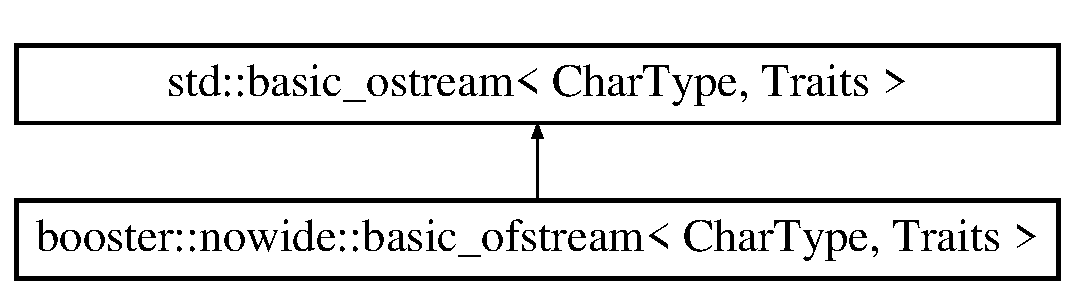
\includegraphics[height=2.000000cm]{classbooster_1_1nowide_1_1basic__ofstream}
\end{center}
\end{figure}
\subsection*{Public Types}
\begin{DoxyCompactItemize}
\item 
typedef {\bf basic\+\_\+filebuf}$<$ Char\+Type, Traits $>$ {\bfseries internal\+\_\+buffer\+\_\+type}\label{classbooster_1_1nowide_1_1basic__ofstream_abb81c9368f20f17ace9841b4153723c8}

\item 
typedef std\+::basic\+\_\+ostream$<$ Char\+Type, Traits $>$ {\bfseries internal\+\_\+stream\+\_\+type}\label{classbooster_1_1nowide_1_1basic__ofstream_a4cf9219d4d52d5598ad7cf55c225d153}

\end{DoxyCompactItemize}
\subsection*{Public Member Functions}
\begin{DoxyCompactItemize}
\item 
{\bfseries basic\+\_\+ofstream} (char const $\ast$file\+\_\+name, std\+::ios\+\_\+base\+::openmode mode=std\+::ios\+\_\+base\+::out)\label{classbooster_1_1nowide_1_1basic__ofstream_ad179dbb18e7d03ac16e49860b53d8d06}

\item 
void {\bfseries open} (char const $\ast$file\+\_\+name, std\+::ios\+\_\+base\+::openmode mode=std\+::ios\+\_\+base\+::out)\label{classbooster_1_1nowide_1_1basic__ofstream_a7c0bbc97ff23f14759536c32777a643f}

\item 
bool {\bfseries is\+\_\+open} ()\label{classbooster_1_1nowide_1_1basic__ofstream_aee64c68ef40f50491942f3b67bb25d3c}

\item 
bool {\bfseries is\+\_\+open} () const \label{classbooster_1_1nowide_1_1basic__ofstream_afbaf63149f90c1f8b07dd00d602f8470}

\item 
void {\bfseries close} ()\label{classbooster_1_1nowide_1_1basic__ofstream_ad7b1e793f9519061b9afca86e6eb587d}

\item 
{\bf internal\+\_\+buffer\+\_\+type} $\ast$ {\bfseries rdbuf} () const \label{classbooster_1_1nowide_1_1basic__ofstream_a339a5fe76e56123ae0095ca98f016866}

\end{DoxyCompactItemize}


\subsection{Detailed Description}
\subsubsection*{template$<$typename Char\+Type, typename Traits = std\+::char\+\_\+traits$<$\+Char\+Type$>$$>$\\*
class booster\+::nowide\+::basic\+\_\+ofstream$<$ Char\+Type, Traits $>$}

Same as std\+::basic\+\_\+ofstream$<$char$>$ but accepts U\+T\+F-\/8 strings under Windows 

The documentation for this class was generated from the following file\+:\begin{DoxyCompactItemize}
\item 
booster/nowide/fstream.\+h\end{DoxyCompactItemize}

\section{booster\+:\+:aio\+:\+:basic\+\_\+socket Class Reference}
\label{classbooster_1_1aio_1_1basic__socket}\index{booster\+::aio\+::basic\+\_\+socket@{booster\+::aio\+::basic\+\_\+socket}}


This class represents a basic Socket object.  




{\ttfamily \#include $<$booster/booster/aio/basic\+\_\+socket.\+h$>$}

Inheritance diagram for booster\+:\+:aio\+:\+:basic\+\_\+socket\+:\begin{figure}[H]
\begin{center}
\leavevmode
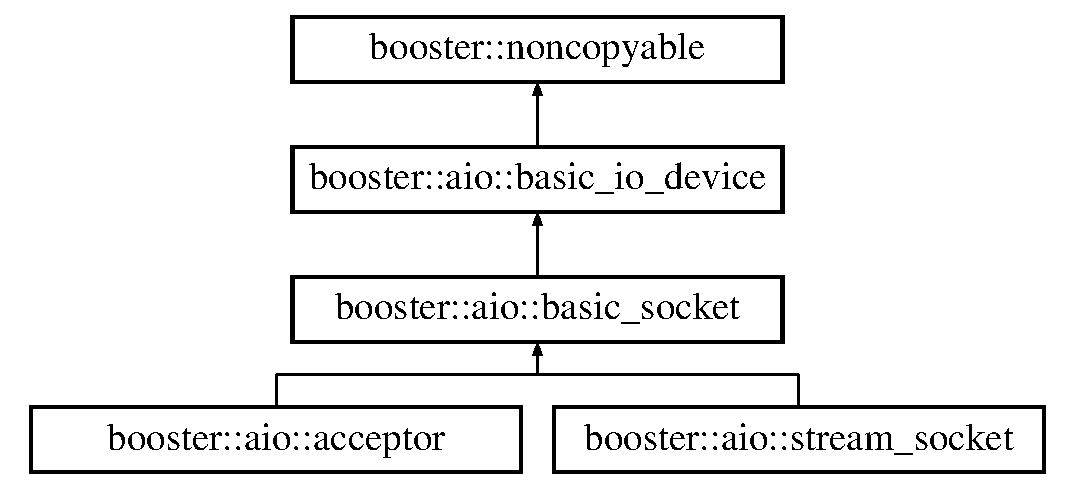
\includegraphics[height=4.000000cm]{classbooster_1_1aio_1_1basic__socket}
\end{center}
\end{figure}
\subsection*{Public Types}
\begin{DoxyCompactItemize}
\item 
enum {\bf boolean\+\_\+option\+\_\+type} \{ {\bfseries tcp\+\_\+no\+\_\+delay}, 
{\bfseries keep\+\_\+alive}, 
{\bfseries reuse\+\_\+address}
 \}
\item 
enum {\bf integer\+\_\+option\+\_\+type} \{ {\bfseries receive\+\_\+buffer\+\_\+size}, 
{\bfseries send\+\_\+buffer\+\_\+size}
 \}
\end{DoxyCompactItemize}
\subsection*{Public Member Functions}
\begin{DoxyCompactItemize}
\item 
{\bf basic\+\_\+socket} ()
\item 
{\bf basic\+\_\+socket} ({\bf io\+\_\+service} \&srv)
\item 
void {\bf open} ({\bf family\+\_\+type} d, {\bf socket\+\_\+type} t)
\item 
void {\bf open} ({\bf family\+\_\+type} d, {\bf socket\+\_\+type} t, system\+::error\+\_\+code \&e)
\item 
{\bf endpoint} {\bf local\+\_\+endpoint} (system\+::error\+\_\+code \&e)
\item 
{\bf endpoint} {\bf local\+\_\+endpoint} ()
\item 
{\bf endpoint} {\bf remote\+\_\+endpoint} (system\+::error\+\_\+code \&e)
\item 
{\bf endpoint} {\bf remote\+\_\+endpoint} ()
\item 
bool {\bf get\+\_\+option} ({\bf boolean\+\_\+option\+\_\+type} opt, system\+::error\+\_\+code \&e)
\item 
bool {\bf get\+\_\+option} ({\bf boolean\+\_\+option\+\_\+type} opt)
\item 
void {\bf set\+\_\+option} ({\bf boolean\+\_\+option\+\_\+type} opt, bool v, system\+::error\+\_\+code \&e)
\item 
void {\bf set\+\_\+option} ({\bf boolean\+\_\+option\+\_\+type} opt, bool v)
\item 
int {\bf get\+\_\+option} ({\bf integer\+\_\+option\+\_\+type} opt, system\+::error\+\_\+code \&e)
\item 
int {\bf get\+\_\+option} ({\bf integer\+\_\+option\+\_\+type} opt)
\item 
void {\bf set\+\_\+option} ({\bf integer\+\_\+option\+\_\+type} opt, int v, system\+::error\+\_\+code \&e)
\item 
void {\bf set\+\_\+option} ({\bf integer\+\_\+option\+\_\+type} opt, int v)
\item 
void {\bf bind} ({\bf endpoint} const \&ep)
\item 
void {\bf bind} ({\bf endpoint} const \&ep, system\+::error\+\_\+code \&e)
\end{DoxyCompactItemize}
\subsection*{Additional Inherited Members}


\subsection{Detailed Description}
This class represents a basic Socket object. 

\subsection{Member Enumeration Documentation}
\index{booster\+::aio\+::basic\+\_\+socket@{booster\+::aio\+::basic\+\_\+socket}!boolean\+\_\+option\+\_\+type@{boolean\+\_\+option\+\_\+type}}
\index{boolean\+\_\+option\+\_\+type@{boolean\+\_\+option\+\_\+type}!booster\+::aio\+::basic\+\_\+socket@{booster\+::aio\+::basic\+\_\+socket}}
\subsubsection[{boolean\+\_\+option\+\_\+type}]{\setlength{\rightskip}{0pt plus 5cm}enum {\bf booster\+::aio\+::basic\+\_\+socket\+::boolean\+\_\+option\+\_\+type}}\label{classbooster_1_1aio_1_1basic__socket_ab60864711436fd648ed7235a4295f28b}
Boolean socket options list \index{booster\+::aio\+::basic\+\_\+socket@{booster\+::aio\+::basic\+\_\+socket}!integer\+\_\+option\+\_\+type@{integer\+\_\+option\+\_\+type}}
\index{integer\+\_\+option\+\_\+type@{integer\+\_\+option\+\_\+type}!booster\+::aio\+::basic\+\_\+socket@{booster\+::aio\+::basic\+\_\+socket}}
\subsubsection[{integer\+\_\+option\+\_\+type}]{\setlength{\rightskip}{0pt plus 5cm}enum {\bf booster\+::aio\+::basic\+\_\+socket\+::integer\+\_\+option\+\_\+type}}\label{classbooster_1_1aio_1_1basic__socket_a139fcb4f3eae7059a716c7822d693ce6}
Integer socket options list

\doxyref{New in Cpp\+C\+MS 1.\+2}{p.}{v1_2} 

\subsection{Constructor \& Destructor Documentation}
\index{booster\+::aio\+::basic\+\_\+socket@{booster\+::aio\+::basic\+\_\+socket}!basic\+\_\+socket@{basic\+\_\+socket}}
\index{basic\+\_\+socket@{basic\+\_\+socket}!booster\+::aio\+::basic\+\_\+socket@{booster\+::aio\+::basic\+\_\+socket}}
\subsubsection[{basic\+\_\+socket()}]{\setlength{\rightskip}{0pt plus 5cm}booster\+::aio\+::basic\+\_\+socket\+::basic\+\_\+socket (
\begin{DoxyParamCaption}
{}
\end{DoxyParamCaption}
)}\label{classbooster_1_1aio_1_1basic__socket_a50acca0717c6d4f404b62eff5f560085}
Create a new socket object \index{booster\+::aio\+::basic\+\_\+socket@{booster\+::aio\+::basic\+\_\+socket}!basic\+\_\+socket@{basic\+\_\+socket}}
\index{basic\+\_\+socket@{basic\+\_\+socket}!booster\+::aio\+::basic\+\_\+socket@{booster\+::aio\+::basic\+\_\+socket}}
\subsubsection[{basic\+\_\+socket(io\+\_\+service \&srv)}]{\setlength{\rightskip}{0pt plus 5cm}booster\+::aio\+::basic\+\_\+socket\+::basic\+\_\+socket (
\begin{DoxyParamCaption}
\item[{{\bf io\+\_\+service} \&}]{srv}
\end{DoxyParamCaption}
)}\label{classbooster_1_1aio_1_1basic__socket_a99abb7e089a806edac4b47b839c6c363}
Create a new socket object and connect to the \doxyref{io\+\_\+service}{p.}{classbooster_1_1aio_1_1io__service} {\itshape srv} 

\subsection{Member Function Documentation}
\index{booster\+::aio\+::basic\+\_\+socket@{booster\+::aio\+::basic\+\_\+socket}!bind@{bind}}
\index{bind@{bind}!booster\+::aio\+::basic\+\_\+socket@{booster\+::aio\+::basic\+\_\+socket}}
\subsubsection[{bind(endpoint const \&ep)}]{\setlength{\rightskip}{0pt plus 5cm}void booster\+::aio\+::basic\+\_\+socket\+::bind (
\begin{DoxyParamCaption}
\item[{{\bf endpoint} const \&}]{ep}
\end{DoxyParamCaption}
)}\label{classbooster_1_1aio_1_1basic__socket_a0f5af05e39968020313bd0e942f542d1}
Bind the opended socket the \doxyref{endpoint}{p.}{classbooster_1_1aio_1_1endpoint} {\itshape ep} 

Throws system\+::system\+\_\+error if error occurs.

\doxyref{New in Cpp\+C\+MS 1.\+2}{p.}{v1_2} \index{booster\+::aio\+::basic\+\_\+socket@{booster\+::aio\+::basic\+\_\+socket}!bind@{bind}}
\index{bind@{bind}!booster\+::aio\+::basic\+\_\+socket@{booster\+::aio\+::basic\+\_\+socket}}
\subsubsection[{bind(endpoint const \&ep, system\+::error\+\_\+code \&e)}]{\setlength{\rightskip}{0pt plus 5cm}void booster\+::aio\+::basic\+\_\+socket\+::bind (
\begin{DoxyParamCaption}
\item[{{\bf endpoint} const \&}]{ep, }
\item[{system\+::error\+\_\+code \&}]{e}
\end{DoxyParamCaption}
)}\label{classbooster_1_1aio_1_1basic__socket_adbf4d4ea4be301d43aff22bfe8167038}
Bind the opended socket the \doxyref{endpoint}{p.}{classbooster_1_1aio_1_1endpoint} {\itshape ep} 

If a error occurs it is assigned to {\itshape e}.

\doxyref{New in Cpp\+C\+MS 1.\+2}{p.}{v1_2} \index{booster\+::aio\+::basic\+\_\+socket@{booster\+::aio\+::basic\+\_\+socket}!get\+\_\+option@{get\+\_\+option}}
\index{get\+\_\+option@{get\+\_\+option}!booster\+::aio\+::basic\+\_\+socket@{booster\+::aio\+::basic\+\_\+socket}}
\subsubsection[{get\+\_\+option(boolean\+\_\+option\+\_\+type opt, system\+::error\+\_\+code \&e)}]{\setlength{\rightskip}{0pt plus 5cm}bool booster\+::aio\+::basic\+\_\+socket\+::get\+\_\+option (
\begin{DoxyParamCaption}
\item[{{\bf boolean\+\_\+option\+\_\+type}}]{opt, }
\item[{system\+::error\+\_\+code \&}]{e}
\end{DoxyParamCaption}
)}\label{classbooster_1_1aio_1_1basic__socket_ad6052ec984f273427d6d5f2bef23336c}
Get a value for a boolean\+\_\+option\+\_\+type

If a error occurs it is assigned to {\itshape e}. \index{booster\+::aio\+::basic\+\_\+socket@{booster\+::aio\+::basic\+\_\+socket}!get\+\_\+option@{get\+\_\+option}}
\index{get\+\_\+option@{get\+\_\+option}!booster\+::aio\+::basic\+\_\+socket@{booster\+::aio\+::basic\+\_\+socket}}
\subsubsection[{get\+\_\+option(boolean\+\_\+option\+\_\+type opt)}]{\setlength{\rightskip}{0pt plus 5cm}bool booster\+::aio\+::basic\+\_\+socket\+::get\+\_\+option (
\begin{DoxyParamCaption}
\item[{{\bf boolean\+\_\+option\+\_\+type}}]{opt}
\end{DoxyParamCaption}
)}\label{classbooster_1_1aio_1_1basic__socket_a1be5a4cf77c1b066f45ba06d92ac43e6}
Get a value for a boolean\+\_\+option\+\_\+type Throws system\+::system\+\_\+error if error occurs. \index{booster\+::aio\+::basic\+\_\+socket@{booster\+::aio\+::basic\+\_\+socket}!get\+\_\+option@{get\+\_\+option}}
\index{get\+\_\+option@{get\+\_\+option}!booster\+::aio\+::basic\+\_\+socket@{booster\+::aio\+::basic\+\_\+socket}}
\subsubsection[{get\+\_\+option(integer\+\_\+option\+\_\+type opt, system\+::error\+\_\+code \&e)}]{\setlength{\rightskip}{0pt plus 5cm}int booster\+::aio\+::basic\+\_\+socket\+::get\+\_\+option (
\begin{DoxyParamCaption}
\item[{{\bf integer\+\_\+option\+\_\+type}}]{opt, }
\item[{system\+::error\+\_\+code \&}]{e}
\end{DoxyParamCaption}
)}\label{classbooster_1_1aio_1_1basic__socket_af62be94433c01655eb7130bad157dcfb}
Get a value for a integer\+\_\+option\+\_\+type

If a error occurs it is assigned to {\itshape e}.

\doxyref{New in Cpp\+C\+MS 1.\+2}{p.}{v1_2} \index{booster\+::aio\+::basic\+\_\+socket@{booster\+::aio\+::basic\+\_\+socket}!get\+\_\+option@{get\+\_\+option}}
\index{get\+\_\+option@{get\+\_\+option}!booster\+::aio\+::basic\+\_\+socket@{booster\+::aio\+::basic\+\_\+socket}}
\subsubsection[{get\+\_\+option(integer\+\_\+option\+\_\+type opt)}]{\setlength{\rightskip}{0pt plus 5cm}int booster\+::aio\+::basic\+\_\+socket\+::get\+\_\+option (
\begin{DoxyParamCaption}
\item[{{\bf integer\+\_\+option\+\_\+type}}]{opt}
\end{DoxyParamCaption}
)}\label{classbooster_1_1aio_1_1basic__socket_a0523c17612c3d5a8108e170d85dbf34e}
Get a value for a integer\+\_\+option\+\_\+type Throws system\+::system\+\_\+error if error occurs.

\doxyref{New in Cpp\+C\+MS 1.\+2}{p.}{v1_2} \index{booster\+::aio\+::basic\+\_\+socket@{booster\+::aio\+::basic\+\_\+socket}!local\+\_\+endpoint@{local\+\_\+endpoint}}
\index{local\+\_\+endpoint@{local\+\_\+endpoint}!booster\+::aio\+::basic\+\_\+socket@{booster\+::aio\+::basic\+\_\+socket}}
\subsubsection[{local\+\_\+endpoint(system\+::error\+\_\+code \&e)}]{\setlength{\rightskip}{0pt plus 5cm}{\bf endpoint} booster\+::aio\+::basic\+\_\+socket\+::local\+\_\+endpoint (
\begin{DoxyParamCaption}
\item[{system\+::error\+\_\+code \&}]{e}
\end{DoxyParamCaption}
)}\label{classbooster_1_1aio_1_1basic__socket_af878ef58d67c2f8c3f29374ae80cf6f9}
Get a local endpoint for the socket

If a error occurs it is assigned to {\itshape e}. \index{booster\+::aio\+::basic\+\_\+socket@{booster\+::aio\+::basic\+\_\+socket}!local\+\_\+endpoint@{local\+\_\+endpoint}}
\index{local\+\_\+endpoint@{local\+\_\+endpoint}!booster\+::aio\+::basic\+\_\+socket@{booster\+::aio\+::basic\+\_\+socket}}
\subsubsection[{local\+\_\+endpoint()}]{\setlength{\rightskip}{0pt plus 5cm}{\bf endpoint} booster\+::aio\+::basic\+\_\+socket\+::local\+\_\+endpoint (
\begin{DoxyParamCaption}
{}
\end{DoxyParamCaption}
)}\label{classbooster_1_1aio_1_1basic__socket_a71260a04f3b934a8da0b6ea7b6c58262}
Get a local endpoint for the socket

Throws system\+::system\+\_\+error if error occurs. \index{booster\+::aio\+::basic\+\_\+socket@{booster\+::aio\+::basic\+\_\+socket}!open@{open}}
\index{open@{open}!booster\+::aio\+::basic\+\_\+socket@{booster\+::aio\+::basic\+\_\+socket}}
\subsubsection[{open(family\+\_\+type d, socket\+\_\+type t)}]{\setlength{\rightskip}{0pt plus 5cm}void booster\+::aio\+::basic\+\_\+socket\+::open (
\begin{DoxyParamCaption}
\item[{{\bf family\+\_\+type}}]{d, }
\item[{{\bf socket\+\_\+type}}]{t}
\end{DoxyParamCaption}
)}\label{classbooster_1_1aio_1_1basic__socket_a44e1dd60570723ab3ba8eebe375f5d62}
Open a socket of \doxyref{family\+\_\+type}{p.}{namespacebooster_1_1aio_a272e1f9b8b2b4e0cf3289749cd51baaa} {\itshape d} and of the protocol (\doxyref{socket\+\_\+type}{p.}{namespacebooster_1_1aio_a0416bbe59893fe8f42b1a12fad7f6e10}) {\itshape t} 

Throws system\+::system\+\_\+error if error occurs. \index{booster\+::aio\+::basic\+\_\+socket@{booster\+::aio\+::basic\+\_\+socket}!open@{open}}
\index{open@{open}!booster\+::aio\+::basic\+\_\+socket@{booster\+::aio\+::basic\+\_\+socket}}
\subsubsection[{open(family\+\_\+type d, socket\+\_\+type t, system\+::error\+\_\+code \&e)}]{\setlength{\rightskip}{0pt plus 5cm}void booster\+::aio\+::basic\+\_\+socket\+::open (
\begin{DoxyParamCaption}
\item[{{\bf family\+\_\+type}}]{d, }
\item[{{\bf socket\+\_\+type}}]{t, }
\item[{system\+::error\+\_\+code \&}]{e}
\end{DoxyParamCaption}
)}\label{classbooster_1_1aio_1_1basic__socket_a487cedd7f1699fb41e224da2c3d717c2}
Opens a new stream socket of a \doxyref{family\+\_\+type}{p.}{namespacebooster_1_1aio_a272e1f9b8b2b4e0cf3289749cd51baaa} {\itshape d} 

If a error occurs it is assigned to {\itshape e}. \index{booster\+::aio\+::basic\+\_\+socket@{booster\+::aio\+::basic\+\_\+socket}!remote\+\_\+endpoint@{remote\+\_\+endpoint}}
\index{remote\+\_\+endpoint@{remote\+\_\+endpoint}!booster\+::aio\+::basic\+\_\+socket@{booster\+::aio\+::basic\+\_\+socket}}
\subsubsection[{remote\+\_\+endpoint(system\+::error\+\_\+code \&e)}]{\setlength{\rightskip}{0pt plus 5cm}{\bf endpoint} booster\+::aio\+::basic\+\_\+socket\+::remote\+\_\+endpoint (
\begin{DoxyParamCaption}
\item[{system\+::error\+\_\+code \&}]{e}
\end{DoxyParamCaption}
)}\label{classbooster_1_1aio_1_1basic__socket_aa84287670c2b47389f756ca7a803e409}
Get a remote endpoint for the socket

If a error occurs it is assigned to {\itshape e}. \index{booster\+::aio\+::basic\+\_\+socket@{booster\+::aio\+::basic\+\_\+socket}!remote\+\_\+endpoint@{remote\+\_\+endpoint}}
\index{remote\+\_\+endpoint@{remote\+\_\+endpoint}!booster\+::aio\+::basic\+\_\+socket@{booster\+::aio\+::basic\+\_\+socket}}
\subsubsection[{remote\+\_\+endpoint()}]{\setlength{\rightskip}{0pt plus 5cm}{\bf endpoint} booster\+::aio\+::basic\+\_\+socket\+::remote\+\_\+endpoint (
\begin{DoxyParamCaption}
{}
\end{DoxyParamCaption}
)}\label{classbooster_1_1aio_1_1basic__socket_a3df0c49be90438df9a30b3854d35deb8}
Get a remote endpoint for the socket

Throws system\+::system\+\_\+error if error occurs. \index{booster\+::aio\+::basic\+\_\+socket@{booster\+::aio\+::basic\+\_\+socket}!set\+\_\+option@{set\+\_\+option}}
\index{set\+\_\+option@{set\+\_\+option}!booster\+::aio\+::basic\+\_\+socket@{booster\+::aio\+::basic\+\_\+socket}}
\subsubsection[{set\+\_\+option(boolean\+\_\+option\+\_\+type opt, bool v, system\+::error\+\_\+code \&e)}]{\setlength{\rightskip}{0pt plus 5cm}void booster\+::aio\+::basic\+\_\+socket\+::set\+\_\+option (
\begin{DoxyParamCaption}
\item[{{\bf boolean\+\_\+option\+\_\+type}}]{opt, }
\item[{bool}]{v, }
\item[{system\+::error\+\_\+code \&}]{e}
\end{DoxyParamCaption}
)}\label{classbooster_1_1aio_1_1basic__socket_a7548662a981240cfb5e2f5ca1614f21f}
Set a value for a boolean\+\_\+option\+\_\+type

If a error occurs it is assigned to {\itshape e}. \index{booster\+::aio\+::basic\+\_\+socket@{booster\+::aio\+::basic\+\_\+socket}!set\+\_\+option@{set\+\_\+option}}
\index{set\+\_\+option@{set\+\_\+option}!booster\+::aio\+::basic\+\_\+socket@{booster\+::aio\+::basic\+\_\+socket}}
\subsubsection[{set\+\_\+option(boolean\+\_\+option\+\_\+type opt, bool v)}]{\setlength{\rightskip}{0pt plus 5cm}void booster\+::aio\+::basic\+\_\+socket\+::set\+\_\+option (
\begin{DoxyParamCaption}
\item[{{\bf boolean\+\_\+option\+\_\+type}}]{opt, }
\item[{bool}]{v}
\end{DoxyParamCaption}
)}\label{classbooster_1_1aio_1_1basic__socket_a19bfa7308302334af52dd2b9e69b01e0}
Set a value for a boolean\+\_\+option\+\_\+type

Throws system\+::system\+\_\+error if error occurs. \index{booster\+::aio\+::basic\+\_\+socket@{booster\+::aio\+::basic\+\_\+socket}!set\+\_\+option@{set\+\_\+option}}
\index{set\+\_\+option@{set\+\_\+option}!booster\+::aio\+::basic\+\_\+socket@{booster\+::aio\+::basic\+\_\+socket}}
\subsubsection[{set\+\_\+option(integer\+\_\+option\+\_\+type opt, int v, system\+::error\+\_\+code \&e)}]{\setlength{\rightskip}{0pt plus 5cm}void booster\+::aio\+::basic\+\_\+socket\+::set\+\_\+option (
\begin{DoxyParamCaption}
\item[{{\bf integer\+\_\+option\+\_\+type}}]{opt, }
\item[{int}]{v, }
\item[{system\+::error\+\_\+code \&}]{e}
\end{DoxyParamCaption}
)}\label{classbooster_1_1aio_1_1basic__socket_a6505967b7ee3a14ff2b6ab56bb6b68c4}
Set a value for a integer\+\_\+option\+\_\+type

If a error occurs it is assigned to {\itshape e}.

\doxyref{New in Cpp\+C\+MS 1.\+2}{p.}{v1_2} \index{booster\+::aio\+::basic\+\_\+socket@{booster\+::aio\+::basic\+\_\+socket}!set\+\_\+option@{set\+\_\+option}}
\index{set\+\_\+option@{set\+\_\+option}!booster\+::aio\+::basic\+\_\+socket@{booster\+::aio\+::basic\+\_\+socket}}
\subsubsection[{set\+\_\+option(integer\+\_\+option\+\_\+type opt, int v)}]{\setlength{\rightskip}{0pt plus 5cm}void booster\+::aio\+::basic\+\_\+socket\+::set\+\_\+option (
\begin{DoxyParamCaption}
\item[{{\bf integer\+\_\+option\+\_\+type}}]{opt, }
\item[{int}]{v}
\end{DoxyParamCaption}
)}\label{classbooster_1_1aio_1_1basic__socket_a9e6a37b2edfd9681818adad5bfac5a91}
Set a value for a integer\+\_\+option\+\_\+type

Throws system\+::system\+\_\+error if error occurs.

\doxyref{New in Cpp\+C\+MS 1.\+2}{p.}{v1_2} 

The documentation for this class was generated from the following file\+:\begin{DoxyCompactItemize}
\item 
booster/aio/basic\+\_\+socket.\+h\end{DoxyCompactItemize}

\section{booster\+:\+:aio\+:\+:buffer\+\_\+impl$<$ Pointer $>$ Class Template Reference}
\label{classbooster_1_1aio_1_1buffer__impl}\index{booster\+::aio\+::buffer\+\_\+impl$<$ Pointer $>$@{booster\+::aio\+::buffer\+\_\+impl$<$ Pointer $>$}}


This is a base class that represents a buffer -\/ a set of contiguous chunks of memory that can be transfered over network.  




{\ttfamily \#include $<$booster/booster/aio/buffer.\+h$>$}

\subsection*{Classes}
\begin{DoxyCompactItemize}
\item 
struct {\bf entry}
\end{DoxyCompactItemize}
\subsection*{Public Types}
\begin{DoxyCompactItemize}
\item 
typedef std\+::pair$<$ {\bf entry} const $\ast$, size\+\_\+t $>$ {\bf buffer\+\_\+data\+\_\+type}\label{classbooster_1_1aio_1_1buffer__impl_af62874c2d9d31b2b3de2a1a8ad1021f1}

\begin{DoxyCompactList}\small\item\em A pair that defined the chunk. \end{DoxyCompactList}\end{DoxyCompactItemize}
\subsection*{Public Member Functions}
\begin{DoxyCompactItemize}
\item 
{\bf buffer\+\_\+impl} ()
\item 
std\+::pair$<$ {\bf entry} const $\ast$, size\+\_\+t $>$ {\bf get} () const 
\item 
void {\bf add} (Pointer p, size\+\_\+t s)
\item 
bool {\bf empty} () const 
\item 
size\+\_\+t {\bf size} () const 
\item 
size\+\_\+t {\bf bytes\+\_\+count} () const 
\end{DoxyCompactItemize}


\subsection{Detailed Description}
\subsubsection*{template$<$typename Pointer$>$\\*
class booster\+::aio\+::buffer\+\_\+impl$<$ Pointer $>$}

This is a base class that represents a buffer -\/ a set of contiguous chunks of memory that can be transfered over network. 

The {\itshape Pointer} parameter should be either {\ttfamily char const $\ast$} or {\ttfamily char $\ast$} 

\subsection{Constructor \& Destructor Documentation}
\index{booster\+::aio\+::buffer\+\_\+impl@{booster\+::aio\+::buffer\+\_\+impl}!buffer\+\_\+impl@{buffer\+\_\+impl}}
\index{buffer\+\_\+impl@{buffer\+\_\+impl}!booster\+::aio\+::buffer\+\_\+impl@{booster\+::aio\+::buffer\+\_\+impl}}
\subsubsection[{buffer\+\_\+impl()}]{\setlength{\rightskip}{0pt plus 5cm}template$<$typename Pointer$>$ {\bf booster\+::aio\+::buffer\+\_\+impl}$<$ Pointer $>$\+::{\bf buffer\+\_\+impl} (
\begin{DoxyParamCaption}
{}
\end{DoxyParamCaption}
)\hspace{0.3cm}{\ttfamily [inline]}}\label{classbooster_1_1aio_1_1buffer__impl_adba3a72dbe48a73a1cc7173b224a7a8d}
Create an empty buffer 

\subsection{Member Function Documentation}
\index{booster\+::aio\+::buffer\+\_\+impl@{booster\+::aio\+::buffer\+\_\+impl}!add@{add}}
\index{add@{add}!booster\+::aio\+::buffer\+\_\+impl@{booster\+::aio\+::buffer\+\_\+impl}}
\subsubsection[{add(\+Pointer p, size\+\_\+t s)}]{\setlength{\rightskip}{0pt plus 5cm}template$<$typename Pointer$>$ void {\bf booster\+::aio\+::buffer\+\_\+impl}$<$ Pointer $>$\+::add (
\begin{DoxyParamCaption}
\item[{Pointer}]{p, }
\item[{size\+\_\+t}]{s}
\end{DoxyParamCaption}
)\hspace{0.3cm}{\ttfamily [inline]}}\label{classbooster_1_1aio_1_1buffer__impl_ac60e6ab00fa30929d7174aae1ddd683d}
Append a chunk to the buffer 

Referenced by booster\+::aio\+::buffer(), and booster\+::aio\+::const\+\_\+buffer\+::const\+\_\+buffer().

\index{booster\+::aio\+::buffer\+\_\+impl@{booster\+::aio\+::buffer\+\_\+impl}!bytes\+\_\+count@{bytes\+\_\+count}}
\index{bytes\+\_\+count@{bytes\+\_\+count}!booster\+::aio\+::buffer\+\_\+impl@{booster\+::aio\+::buffer\+\_\+impl}}
\subsubsection[{bytes\+\_\+count() const }]{\setlength{\rightskip}{0pt plus 5cm}template$<$typename Pointer$>$ size\+\_\+t {\bf booster\+::aio\+::buffer\+\_\+impl}$<$ Pointer $>$\+::bytes\+\_\+count (
\begin{DoxyParamCaption}
{}
\end{DoxyParamCaption}
) const\hspace{0.3cm}{\ttfamily [inline]}}\label{classbooster_1_1aio_1_1buffer__impl_ab57dec2dc3eb4abbca0e5e4a3eddd36a}
Get total amount of bytes in the buffer

\doxyref{New in Cpp\+C\+MS 1.\+2}{p.}{v1_2} \index{booster\+::aio\+::buffer\+\_\+impl@{booster\+::aio\+::buffer\+\_\+impl}!empty@{empty}}
\index{empty@{empty}!booster\+::aio\+::buffer\+\_\+impl@{booster\+::aio\+::buffer\+\_\+impl}}
\subsubsection[{empty() const }]{\setlength{\rightskip}{0pt plus 5cm}template$<$typename Pointer$>$ bool {\bf booster\+::aio\+::buffer\+\_\+impl}$<$ Pointer $>$\+::empty (
\begin{DoxyParamCaption}
{}
\end{DoxyParamCaption}
) const\hspace{0.3cm}{\ttfamily [inline]}}\label{classbooster_1_1aio_1_1buffer__impl_a239dddcd9990cb80dfbd1b4e88fdc45e}
Check if the buffer is empty \index{booster\+::aio\+::buffer\+\_\+impl@{booster\+::aio\+::buffer\+\_\+impl}!get@{get}}
\index{get@{get}!booster\+::aio\+::buffer\+\_\+impl@{booster\+::aio\+::buffer\+\_\+impl}}
\subsubsection[{get() const }]{\setlength{\rightskip}{0pt plus 5cm}template$<$typename Pointer$>$ std\+::pair$<${\bf entry} const $\ast$,size\+\_\+t$>$ {\bf booster\+::aio\+::buffer\+\_\+impl}$<$ Pointer $>$\+::get (
\begin{DoxyParamCaption}
{}
\end{DoxyParamCaption}
) const\hspace{0.3cm}{\ttfamily [inline]}}\label{classbooster_1_1aio_1_1buffer__impl_af890c2c31103ae60a44a23d69242345e}
Get a first chunk 

Referenced by booster\+::aio\+::buffer(), and booster\+::aio\+::const\+\_\+buffer\+::const\+\_\+buffer().

\index{booster\+::aio\+::buffer\+\_\+impl@{booster\+::aio\+::buffer\+\_\+impl}!size@{size}}
\index{size@{size}!booster\+::aio\+::buffer\+\_\+impl@{booster\+::aio\+::buffer\+\_\+impl}}
\subsubsection[{size() const }]{\setlength{\rightskip}{0pt plus 5cm}template$<$typename Pointer$>$ size\+\_\+t {\bf booster\+::aio\+::buffer\+\_\+impl}$<$ Pointer $>$\+::size (
\begin{DoxyParamCaption}
{}
\end{DoxyParamCaption}
) const\hspace{0.3cm}{\ttfamily [inline]}}\label{classbooster_1_1aio_1_1buffer__impl_aff278bb6f49b84fcfe974aa0b0c8c21c}
Get size of buffer in number of chunks,i.\+e.

\doxyref{New in Cpp\+C\+MS 1.\+2}{p.}{v1_2} 

The documentation for this class was generated from the following file\+:\begin{DoxyCompactItemize}
\item 
booster/aio/buffer.\+h\end{DoxyCompactItemize}

\section{cppcms\+:\+:cache\+\_\+interface Class Reference}
\label{classcppcms_1_1cache__interface}\index{cppcms\+::cache\+\_\+interface@{cppcms\+::cache\+\_\+interface}}


This class is the major gateway of the application to Cpp\+C\+MS caching abilities. Any access too cache would be done via this class.  




{\ttfamily \#include $<$cppcms/cache\+\_\+interface.\+h$>$}

Inheritance diagram for cppcms\+:\+:cache\+\_\+interface\+:\begin{figure}[H]
\begin{center}
\leavevmode
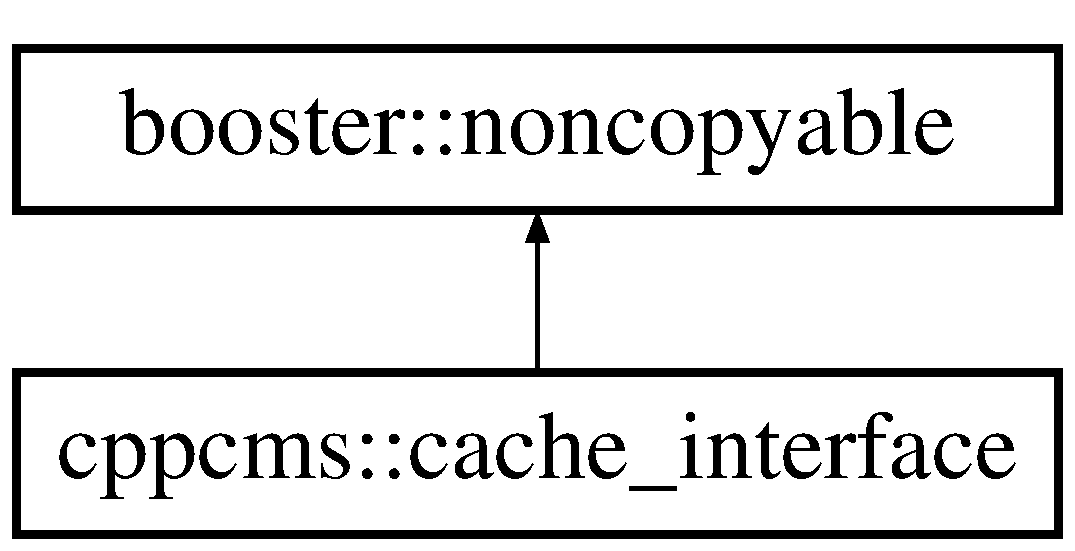
\includegraphics[height=2.000000cm]{classcppcms_1_1cache__interface}
\end{center}
\end{figure}
\subsection*{Public Member Functions}
\begin{DoxyCompactItemize}
\item 
{\bf cache\+\_\+interface} ({\bf cppcms\+::service} \&srv)
\item 
void {\bf rise} (std\+::string const \&trigger)
\item 
void {\bf add\+\_\+trigger} (std\+::string const \&trigger)
\item 
void {\bf clear} ()
\item 
void {\bf reset} ()
\item 
bool {\bf stats} (unsigned \&keys, unsigned \&triggers)
\item 
bool {\bf has\+\_\+cache} ()
\item 
bool {\bf nocache} ()
\item 
bool {\bf fetch\+\_\+page} (std\+::string const \&key)
\item 
void {\bf store\+\_\+page} (std\+::string const \&key, int timeout=-\/1)
\item 
bool {\bf fetch\+\_\+frame} (std\+::string const \&key, std\+::string \&result, bool notriggers=false)
\item 
void {\bf store\+\_\+frame} (std\+::string const \&key, std\+::string const \&frame, std\+::set$<$ std\+::string $>$ const \&triggers=std\+::set$<$ std\+::string $>$(), int timeout=-\/1, bool notriggers=false)
\item 
void {\bf store\+\_\+frame} (std\+::string const \&key, std\+::string const \&frame, int timeout, bool notriggers=false)
\item 
{\footnotesize template$<$typename Serializable $>$ }\\bool {\bf fetch\+\_\+data} (std\+::string const \&key, Serializable \&data, bool notriggers=false)
\item 
{\footnotesize template$<$typename Serializable $>$ }\\void {\bf store\+\_\+data} (std\+::string const \&key, Serializable const \&data, std\+::set$<$ std\+::string $>$ const \&triggers=std\+::set$<$ std\+::string $>$(), int timeout=-\/1, bool notriggers=false)
\item 
{\footnotesize template$<$typename Serializable $>$ }\\void {\bf store\+\_\+data} (std\+::string const \&key, Serializable const \&data, int timeout, bool notriggers=false)
\end{DoxyCompactItemize}
\subsection*{Friends}
\begin{DoxyCompactItemize}
\item 
class {\bfseries triggers\+\_\+recorder}\label{classcppcms_1_1cache__interface_a2b9a3918416586289327d30cb43172df}

\end{DoxyCompactItemize}


\subsection{Detailed Description}
This class is the major gateway of the application to Cpp\+C\+MS caching abilities. Any access too cache would be done via this class. 

Cpp\+C\+MS cache model supports following concepts\+:


\begin{DoxyItemize}
\item {\itshape key} the unique identification of the object in cache
\item {\itshape timeout} -- the maximal time the cached object remains valid
\item {\itshape trigger} -- special key that allows fast invalidation of multiple cache objects.
\end{DoxyItemize}

The first two concepts are quite popular and available in most of Web framework, but the last one is very unique to Cpp\+C\+MS that gives fine grained cache invalidation tools.

Each time the page is created it automatically receives some triggers during the process of creation. When some object is fetched from the cache or stored into it, it adds triggers to the major page. This provides semi-\/automatic triggers management.

For example\+:


\begin{DoxyCode}
 \textcolor{keywordflow}{if}(cache().fetch_page(\textcolor{stringliteral}{"main\_page"}))
   \textcolor{keywordflow}{return};
\textcolor{keywordflow}{if}(!cache().fetch_frame(\textcolor{stringliteral}{"article\_"}+\textcolor{keywordtype}{id},article)) \{
   article=generate\_article\_from\_data\_base(\textcolor{keywordtype}{id});
   cache.store\_frame(\textcolor{stringliteral}{"article\_"}+\textcolor{keywordtype}{id},article);
 \}
 \textcolor{comment}{// Generate some HTML here using article }
 cache.store\_page(\textcolor{stringliteral}{"main"});
\end{DoxyCode}


Let\textquotesingle{}s assume that \char`\"{}main\+\_\+page\char`\"{} wasn\textquotesingle{}t found in cache, then we try to fetch a frame that holds only a single article \char`\"{}article\+\_\+123\char`\"{}, if it is fetched, the result is stored in a string article and the trigger \char`\"{}article\+\_\+123\char`\"{} is automatically added to set of triggers that \char`\"{}main\+\_\+page\char`\"{} depends on them.

When the article updated, and \char`\"{}article\+\_\+123\char`\"{} key is risen, it would automatically invalidate \char`\"{}main\+\_\+page\char`\"{} as well.

Cpp\+C\+MS \doxyref{cache\+\_\+interface}{p.}{classcppcms_1_1cache__interface} allows storing arbitrary object in cache, For this purpose they should be \char`\"{}serializable\char`\"{}. This can be done by specializing a class cppcms\+::setialization\+\_\+traits 

\subsection{Constructor \& Destructor Documentation}
\index{cppcms\+::cache\+\_\+interface@{cppcms\+::cache\+\_\+interface}!cache\+\_\+interface@{cache\+\_\+interface}}
\index{cache\+\_\+interface@{cache\+\_\+interface}!cppcms\+::cache\+\_\+interface@{cppcms\+::cache\+\_\+interface}}
\subsubsection[{cache\+\_\+interface(cppcms\+::service \&srv)}]{\setlength{\rightskip}{0pt plus 5cm}cppcms\+::cache\+\_\+interface\+::cache\+\_\+interface (
\begin{DoxyParamCaption}
\item[{{\bf cppcms\+::service} \&}]{srv}
\end{DoxyParamCaption}
)}\label{classcppcms_1_1cache__interface_a7276736bc9302f62fcafd33377532751}
Create interface object without a context, everything but fetch\+\_\+page and store\+\_\+page would work, it is not possible to handle pages without full i/o context

\doxyref{New in Cpp\+C\+MS 1.\+2}{p.}{v1_2} 

\subsection{Member Function Documentation}
\index{cppcms\+::cache\+\_\+interface@{cppcms\+::cache\+\_\+interface}!add\+\_\+trigger@{add\+\_\+trigger}}
\index{add\+\_\+trigger@{add\+\_\+trigger}!cppcms\+::cache\+\_\+interface@{cppcms\+::cache\+\_\+interface}}
\subsubsection[{add\+\_\+trigger(std\+::string const \&trigger)}]{\setlength{\rightskip}{0pt plus 5cm}void cppcms\+::cache\+\_\+interface\+::add\+\_\+trigger (
\begin{DoxyParamCaption}
\item[{std\+::string const \&}]{trigger}
\end{DoxyParamCaption}
)}\label{classcppcms_1_1cache__interface_ade0f913aea74b4ebe66c8216f33c2b2a}
Add a trigger {\itshape trigger} to the list of dependencies of current page. \index{cppcms\+::cache\+\_\+interface@{cppcms\+::cache\+\_\+interface}!clear@{clear}}
\index{clear@{clear}!cppcms\+::cache\+\_\+interface@{cppcms\+::cache\+\_\+interface}}
\subsubsection[{clear()}]{\setlength{\rightskip}{0pt plus 5cm}void cppcms\+::cache\+\_\+interface\+::clear (
\begin{DoxyParamCaption}
{}
\end{DoxyParamCaption}
)}\label{classcppcms_1_1cache__interface_a71e212f0774f242d2967e66b88fb6aa6}
Clear all Cpp\+C\+MS cache -\/ use carefully \index{cppcms\+::cache\+\_\+interface@{cppcms\+::cache\+\_\+interface}!fetch\+\_\+data@{fetch\+\_\+data}}
\index{fetch\+\_\+data@{fetch\+\_\+data}!cppcms\+::cache\+\_\+interface@{cppcms\+::cache\+\_\+interface}}
\subsubsection[{fetch\+\_\+data(std\+::string const \&key, Serializable \&data, bool notriggers=false)}]{\setlength{\rightskip}{0pt plus 5cm}template$<$typename Serializable $>$ bool cppcms\+::cache\+\_\+interface\+::fetch\+\_\+data (
\begin{DoxyParamCaption}
\item[{std\+::string const \&}]{key, }
\item[{Serializable \&}]{data, }
\item[{bool}]{notriggers = {\ttfamily false}}
\end{DoxyParamCaption}
)\hspace{0.3cm}{\ttfamily [inline]}}\label{classcppcms_1_1cache__interface_ae6d127d4ee07ebbe3d18012a9c59522c}
Fetch a serializeable object from the cache.


\begin{DoxyParams}{Parameters}
{\em key} & -- the key that uniquely defines the frame. \\
\hline
{\em data} & -- an object store fetched data \\
\hline
{\em notriggers} & -- if true, no triggers that an object is dependent on would be added to dependencies of the current page, otherwise (false, default), the all triggers that the object is dependent on, including the {\itshape key} itself would be added as dependent triggers to current rendered page. \\
\hline
\end{DoxyParams}
\begin{DoxyReturn}{Returns}
returns true if the entry was found. 
\end{DoxyReturn}


References cppcms\+::serialization\+\_\+traits$<$ Object $>$\+::load().

\index{cppcms\+::cache\+\_\+interface@{cppcms\+::cache\+\_\+interface}!fetch\+\_\+frame@{fetch\+\_\+frame}}
\index{fetch\+\_\+frame@{fetch\+\_\+frame}!cppcms\+::cache\+\_\+interface@{cppcms\+::cache\+\_\+interface}}
\subsubsection[{fetch\+\_\+frame(std\+::string const \&key, std\+::string \&result, bool notriggers=false)}]{\setlength{\rightskip}{0pt plus 5cm}bool cppcms\+::cache\+\_\+interface\+::fetch\+\_\+frame (
\begin{DoxyParamCaption}
\item[{std\+::string const \&}]{key, }
\item[{std\+::string \&}]{result, }
\item[{bool}]{notriggers = {\ttfamily false}}
\end{DoxyParamCaption}
)}\label{classcppcms_1_1cache__interface_a25287fde30642730132f58d6ccd77183}
Fetch a string (usually some H\+T\+ML part) from the cache.


\begin{DoxyParams}{Parameters}
{\em key} & -- the key that uniquely defines the frame. \\
\hline
{\em result} & -- string to store fetched value \\
\hline
{\em notriggers} & -- if true, no triggers that a frame is dependent on would be added to dependencies of the current page, otherwise (false, default), the all triggers that page is dependent on, including the {\itshape key} itself would be added as dependent triggers to current rendered page. \\
\hline
\end{DoxyParams}
\begin{DoxyReturn}{Returns}
returns true if the entry was found. 
\end{DoxyReturn}
\index{cppcms\+::cache\+\_\+interface@{cppcms\+::cache\+\_\+interface}!fetch\+\_\+page@{fetch\+\_\+page}}
\index{fetch\+\_\+page@{fetch\+\_\+page}!cppcms\+::cache\+\_\+interface@{cppcms\+::cache\+\_\+interface}}
\subsubsection[{fetch\+\_\+page(std\+::string const \&key)}]{\setlength{\rightskip}{0pt plus 5cm}bool cppcms\+::cache\+\_\+interface\+::fetch\+\_\+page (
\begin{DoxyParamCaption}
\item[{std\+::string const \&}]{key}
\end{DoxyParamCaption}
)}\label{classcppcms_1_1cache__interface_ab3fc6d636f0525d500091b4279821688}
Fetch a page from the cache with a key {\itshape key}. If the page exists, it is written to output and true is returned. Otherwise false is returned. \index{cppcms\+::cache\+\_\+interface@{cppcms\+::cache\+\_\+interface}!has\+\_\+cache@{has\+\_\+cache}}
\index{has\+\_\+cache@{has\+\_\+cache}!cppcms\+::cache\+\_\+interface@{cppcms\+::cache\+\_\+interface}}
\subsubsection[{has\+\_\+cache()}]{\setlength{\rightskip}{0pt plus 5cm}bool cppcms\+::cache\+\_\+interface\+::has\+\_\+cache (
\begin{DoxyParamCaption}
{}
\end{DoxyParamCaption}
)}\label{classcppcms_1_1cache__interface_af004bf7322d1819fa429812329f6eb8a}
Returns true if caching system is enabled \index{cppcms\+::cache\+\_\+interface@{cppcms\+::cache\+\_\+interface}!nocache@{nocache}}
\index{nocache@{nocache}!cppcms\+::cache\+\_\+interface@{cppcms\+::cache\+\_\+interface}}
\subsubsection[{nocache()}]{\setlength{\rightskip}{0pt plus 5cm}bool cppcms\+::cache\+\_\+interface\+::nocache (
\begin{DoxyParamCaption}
{}
\end{DoxyParamCaption}
)}\label{classcppcms_1_1cache__interface_a27fdba45f36dd18a1f622061ca50a3e1}
Opposite of {\itshape has\+\_\+cache} \index{cppcms\+::cache\+\_\+interface@{cppcms\+::cache\+\_\+interface}!reset@{reset}}
\index{reset@{reset}!cppcms\+::cache\+\_\+interface@{cppcms\+::cache\+\_\+interface}}
\subsubsection[{reset()}]{\setlength{\rightskip}{0pt plus 5cm}void cppcms\+::cache\+\_\+interface\+::reset (
\begin{DoxyParamCaption}
{}
\end{DoxyParamCaption}
)}\label{classcppcms_1_1cache__interface_ab609740399d76d2cadbe67b5d7c94e3c}
Remove all triggers added to current page so far \index{cppcms\+::cache\+\_\+interface@{cppcms\+::cache\+\_\+interface}!rise@{rise}}
\index{rise@{rise}!cppcms\+::cache\+\_\+interface@{cppcms\+::cache\+\_\+interface}}
\subsubsection[{rise(std\+::string const \&trigger)}]{\setlength{\rightskip}{0pt plus 5cm}void cppcms\+::cache\+\_\+interface\+::rise (
\begin{DoxyParamCaption}
\item[{std\+::string const \&}]{trigger}
\end{DoxyParamCaption}
)}\label{classcppcms_1_1cache__interface_ab8b0d3640a005269e4c01d5c5be09553}
Rise a trigger {\itshape trigger}. All cached objects that depend on this trigger would be invalidated \index{cppcms\+::cache\+\_\+interface@{cppcms\+::cache\+\_\+interface}!stats@{stats}}
\index{stats@{stats}!cppcms\+::cache\+\_\+interface@{cppcms\+::cache\+\_\+interface}}
\subsubsection[{stats(unsigned \&keys, unsigned \&triggers)}]{\setlength{\rightskip}{0pt plus 5cm}bool cppcms\+::cache\+\_\+interface\+::stats (
\begin{DoxyParamCaption}
\item[{unsigned \&}]{keys, }
\item[{unsigned \&}]{triggers}
\end{DoxyParamCaption}
)}\label{classcppcms_1_1cache__interface_a12fcde54f1aa6f1810b12b8bc88ca7ed}
Get statistics about items stored in cache. May require O(n) complexity, use with care.


\begin{DoxyParams}{Parameters}
{\em keys} & -- the number of items stored in cache \\
\hline
{\em triggers} & -- the number of various triggers existing in the cache.\\
\hline
\end{DoxyParams}
Returns false if caching system is disabled. \index{cppcms\+::cache\+\_\+interface@{cppcms\+::cache\+\_\+interface}!store\+\_\+data@{store\+\_\+data}}
\index{store\+\_\+data@{store\+\_\+data}!cppcms\+::cache\+\_\+interface@{cppcms\+::cache\+\_\+interface}}
\subsubsection[{store\+\_\+data(std\+::string const \&key, Serializable const \&data, std\+::set$<$ std\+::string $>$ const \&triggers=std\+::set$<$ std\+::string $>$(), int timeout=-\/1, bool notriggers=false)}]{\setlength{\rightskip}{0pt plus 5cm}template$<$typename Serializable $>$ void cppcms\+::cache\+\_\+interface\+::store\+\_\+data (
\begin{DoxyParamCaption}
\item[{std\+::string const \&}]{key, }
\item[{Serializable const \&}]{data, }
\item[{std\+::set$<$ std\+::string $>$ const \&}]{triggers = {\ttfamily std\+:\+:set$<$std\+:\+:string$>$()}, }
\item[{int}]{timeout = {\ttfamily -\/1}, }
\item[{bool}]{notriggers = {\ttfamily false}}
\end{DoxyParamCaption}
)\hspace{0.3cm}{\ttfamily [inline]}}\label{classcppcms_1_1cache__interface_a1d7ce108ecc1fbae0368d7c521188561}
Store a serializeable object to the cache.


\begin{DoxyParams}{Parameters}
{\em key} & -- the key that uniquely defines the object. \\
\hline
{\em data} & -- the actual object \\
\hline
{\em triggers} & -- the set of triggers that the key should depend on ({\itshape key} is added automatically) \\
\hline
{\em timeout} & -- maximal object lifetime, -\/1 is infinity \\
\hline
{\em notriggers} & -- if {\itshape notriggers} is true no frame dependent triggers would be added to the current page trigger set. Otherwise (default) current page would depend on the {\itshape key} and {\itshape triggers} as its dependent triggers. \\
\hline
\end{DoxyParams}


References cppcms\+::serialization\+\_\+traits$<$ Object $>$\+::save().

\index{cppcms\+::cache\+\_\+interface@{cppcms\+::cache\+\_\+interface}!store\+\_\+data@{store\+\_\+data}}
\index{store\+\_\+data@{store\+\_\+data}!cppcms\+::cache\+\_\+interface@{cppcms\+::cache\+\_\+interface}}
\subsubsection[{store\+\_\+data(std\+::string const \&key, Serializable const \&data, int timeout, bool notriggers=false)}]{\setlength{\rightskip}{0pt plus 5cm}template$<$typename Serializable $>$ void cppcms\+::cache\+\_\+interface\+::store\+\_\+data (
\begin{DoxyParamCaption}
\item[{std\+::string const \&}]{key, }
\item[{Serializable const \&}]{data, }
\item[{int}]{timeout, }
\item[{bool}]{notriggers = {\ttfamily false}}
\end{DoxyParamCaption}
)\hspace{0.3cm}{\ttfamily [inline]}}\label{classcppcms_1_1cache__interface_a30b038c3933fbb0abe8c8f2dec78703e}
Store a serializeable object to the cache.


\begin{DoxyParams}{Parameters}
{\em key} & -- the key that uniquely defines the object. \\
\hline
{\em data} & -- the actual object \\
\hline
{\em timeout} & -- maximal object lifetime, -\/1 is infinity \\
\hline
{\em notriggers} & -- if {\itshape notriggers} is true {\itshape key} added to the current page trigger set. Otherwise (default) current page would depend on the {\itshape key} \\
\hline
\end{DoxyParams}
\index{cppcms\+::cache\+\_\+interface@{cppcms\+::cache\+\_\+interface}!store\+\_\+frame@{store\+\_\+frame}}
\index{store\+\_\+frame@{store\+\_\+frame}!cppcms\+::cache\+\_\+interface@{cppcms\+::cache\+\_\+interface}}
\subsubsection[{store\+\_\+frame(std\+::string const \&key, std\+::string const \&frame, std\+::set$<$ std\+::string $>$ const \&triggers=std\+::set$<$ std\+::string $>$(), int timeout=-\/1, bool notriggers=false)}]{\setlength{\rightskip}{0pt plus 5cm}void cppcms\+::cache\+\_\+interface\+::store\+\_\+frame (
\begin{DoxyParamCaption}
\item[{std\+::string const \&}]{key, }
\item[{std\+::string const \&}]{frame, }
\item[{std\+::set$<$ std\+::string $>$ const \&}]{triggers = {\ttfamily std\+:\+:set$<$~std\+:\+:string~$>$()}, }
\item[{int}]{timeout = {\ttfamily -\/1}, }
\item[{bool}]{notriggers = {\ttfamily false}}
\end{DoxyParamCaption}
)}\label{classcppcms_1_1cache__interface_ab2cdec66d555a62f64c8d014e32b11e0}
Store a string (usually some H\+T\+ML part) to the cache.


\begin{DoxyParams}{Parameters}
{\em key} & -- the key that uniquely defines the frame. \\
\hline
{\em frame} & -- the actual value \\
\hline
{\em triggers} & -- the set of triggers that the key should depend on ({\itshape key} is added automatically) \\
\hline
{\em timeout} & -- maximal object lifetime, -\/1 is infinity \\
\hline
{\em notriggers} & -- if {\itshape notriggers} is true no frame dependent triggers would be added to the current page trigger set. Otherwise (default) current page would depend on the {\itshape key} and {\itshape triggers} as its dependent triggers. \\
\hline
\end{DoxyParams}
\index{cppcms\+::cache\+\_\+interface@{cppcms\+::cache\+\_\+interface}!store\+\_\+frame@{store\+\_\+frame}}
\index{store\+\_\+frame@{store\+\_\+frame}!cppcms\+::cache\+\_\+interface@{cppcms\+::cache\+\_\+interface}}
\subsubsection[{store\+\_\+frame(std\+::string const \&key, std\+::string const \&frame, int timeout, bool notriggers=false)}]{\setlength{\rightskip}{0pt plus 5cm}void cppcms\+::cache\+\_\+interface\+::store\+\_\+frame (
\begin{DoxyParamCaption}
\item[{std\+::string const \&}]{key, }
\item[{std\+::string const \&}]{frame, }
\item[{int}]{timeout, }
\item[{bool}]{notriggers = {\ttfamily false}}
\end{DoxyParamCaption}
)}\label{classcppcms_1_1cache__interface_a2e5102e99a4bf81c311e3e171a4a5539}
Store a string (usually some H\+T\+ML part) to the cache.


\begin{DoxyParams}{Parameters}
{\em key} & -- the key that uniquely defines the frame. \\
\hline
{\em frame} & -- the actual value \\
\hline
{\em timeout} & -- maximal object lifetime, -\/1 is infinity \\
\hline
{\em notriggers} & -- if {\itshape notriggers} is true {\itshape key} added to the current page trigger set. Otherwise (default) current page would depend on the {\itshape key} \\
\hline
\end{DoxyParams}
\index{cppcms\+::cache\+\_\+interface@{cppcms\+::cache\+\_\+interface}!store\+\_\+page@{store\+\_\+page}}
\index{store\+\_\+page@{store\+\_\+page}!cppcms\+::cache\+\_\+interface@{cppcms\+::cache\+\_\+interface}}
\subsubsection[{store\+\_\+page(std\+::string const \&key, int timeout=-\/1)}]{\setlength{\rightskip}{0pt plus 5cm}void cppcms\+::cache\+\_\+interface\+::store\+\_\+page (
\begin{DoxyParamCaption}
\item[{std\+::string const \&}]{key, }
\item[{int}]{timeout = {\ttfamily -\/1}}
\end{DoxyParamCaption}
)}\label{classcppcms_1_1cache__interface_a5f471a4daf6bd7993e591e461bfd0c99}
Store page with key {\itshape akey} in cache, with timeout {\itshape timeout}.

This function stores a page with dependencies on all triggers that were added so far.


\begin{DoxyParams}{Parameters}
{\em key} & -- the key that defines the cache. \\
\hline
{\em timeout} & -- maximal valid time of the page. {\itshape timeout=-\/1} means infinite. Use with care.\\
\hline
\end{DoxyParams}
Note\+: store\+\_\+page does not rise the trigger {\itshape key}, only replaces the value. 

The documentation for this class was generated from the following file\+:\begin{DoxyCompactItemize}
\item 
cppcms/cache\+\_\+interface.\+h\end{DoxyCompactItemize}

\section{booster\+:\+:locale\+:\+:calendar Class Reference}
\label{classbooster_1_1locale_1_1calendar}\index{booster\+::locale\+::calendar@{booster\+::locale\+::calendar}}


this class provides an access to general calendar information.  




{\ttfamily \#include $<$booster/booster/locale/date\+\_\+time.\+h$>$}

\subsection*{Public Member Functions}
\begin{DoxyCompactItemize}
\item 
{\bf calendar} (std\+::ios\+\_\+base \&ios)
\item 
{\bf calendar} (std\+::locale const \&l, std\+::string const \&zone)
\item 
{\bf calendar} (std\+::locale const \&l)
\item 
{\bf calendar} (std\+::string const \&zone)
\item 
{\bf calendar} ()
\item 
{\bf calendar} ({\bf calendar} const \&other)
\item 
{\bf calendar} const \& {\bf operator=} ({\bf calendar} const \&other)
\item 
int {\bf minimum} ({\bf period\+::period\+\_\+type} f) const 
\item 
int {\bf greatest\+\_\+minimum} ({\bf period\+::period\+\_\+type} f) const 
\item 
int {\bf maximum} ({\bf period\+::period\+\_\+type} f) const 
\item 
int {\bf least\+\_\+maximum} ({\bf period\+::period\+\_\+type} f) const 
\item 
int {\bf first\+\_\+day\+\_\+of\+\_\+week} () const \label{classbooster_1_1locale_1_1calendar_a4d841c494c16326e691c9c1668c5cd0f}

\begin{DoxyCompactList}\small\item\em Get first day of week for specific calendar, for example for US it is 1 -\/ Sunday for France it is 2 -\/ Monday. \end{DoxyCompactList}\item 
std\+::locale {\bf get\+\_\+locale} () const 
\item 
std\+::string {\bf get\+\_\+time\+\_\+zone} () const 
\item 
bool {\bf is\+\_\+gregorian} () const 
\item 
bool {\bf operator==} ({\bf calendar} const \&other) const 
\item 
bool {\bf operator!=} ({\bf calendar} const \&other) const 
\end{DoxyCompactItemize}
\subsection*{Friends}
\begin{DoxyCompactItemize}
\item 
class {\bfseries date\+\_\+time}\label{classbooster_1_1locale_1_1calendar_a7c627d823bfb1186af76ed36016cbb31}

\end{DoxyCompactItemize}


\subsection{Detailed Description}
this class provides an access to general calendar information. 

This information is not connected to specific date but generic to locale, and timezone. It is used in obtaining general information about calendar and is essential for creation of \doxyref{date\+\_\+time}{p.}{classbooster_1_1locale_1_1date__time} objects. 

\subsection{Constructor \& Destructor Documentation}
\index{booster\+::locale\+::calendar@{booster\+::locale\+::calendar}!calendar@{calendar}}
\index{calendar@{calendar}!booster\+::locale\+::calendar@{booster\+::locale\+::calendar}}
\subsubsection[{calendar(std\+::ios\+\_\+base \&ios)}]{\setlength{\rightskip}{0pt plus 5cm}booster\+::locale\+::calendar\+::calendar (
\begin{DoxyParamCaption}
\item[{std\+::ios\+\_\+base \&}]{ios}
\end{DoxyParamCaption}
)}\label{classbooster_1_1locale_1_1calendar_ae7318fd3d9756e98e442a41998763424}
Create calendar taking locale and timezone information from ios\+\_\+base instance.

\begin{DoxyNote}{Note}
throws std\+::bad\+\_\+cast if ios does not have a locale with installed \doxyref{calendar\+\_\+facet}{p.}{classbooster_1_1locale_1_1calendar__facet} facet installed 
\end{DoxyNote}
\index{booster\+::locale\+::calendar@{booster\+::locale\+::calendar}!calendar@{calendar}}
\index{calendar@{calendar}!booster\+::locale\+::calendar@{booster\+::locale\+::calendar}}
\subsubsection[{calendar(std\+::locale const \&l, std\+::string const \&zone)}]{\setlength{\rightskip}{0pt plus 5cm}booster\+::locale\+::calendar\+::calendar (
\begin{DoxyParamCaption}
\item[{std\+::locale const \&}]{l, }
\item[{std\+::string const \&}]{zone}
\end{DoxyParamCaption}
)}\label{classbooster_1_1locale_1_1calendar_aacb45467dbc3832c4b43708600a03f06}
Create calendar with locale {\itshape l} and \doxyref{time\+\_\+zone}{p.}{namespacebooster_1_1locale_1_1time__zone} {\itshape zone} 

\begin{DoxyNote}{Note}
throws std\+::bad\+\_\+cast if loc does not have \doxyref{calendar\+\_\+facet}{p.}{classbooster_1_1locale_1_1calendar__facet} facet installed 
\end{DoxyNote}
\index{booster\+::locale\+::calendar@{booster\+::locale\+::calendar}!calendar@{calendar}}
\index{calendar@{calendar}!booster\+::locale\+::calendar@{booster\+::locale\+::calendar}}
\subsubsection[{calendar(std\+::locale const \&l)}]{\setlength{\rightskip}{0pt plus 5cm}booster\+::locale\+::calendar\+::calendar (
\begin{DoxyParamCaption}
\item[{std\+::locale const \&}]{l}
\end{DoxyParamCaption}
)}\label{classbooster_1_1locale_1_1calendar_a27cb3ad4e768b9a7cbf0c21db2822a15}
Create calendar with locale {\itshape l} and default timezone

\begin{DoxyNote}{Note}
throws std\+::bad\+\_\+cast if loc does not have \doxyref{calendar\+\_\+facet}{p.}{classbooster_1_1locale_1_1calendar__facet} facet installed 
\end{DoxyNote}
\index{booster\+::locale\+::calendar@{booster\+::locale\+::calendar}!calendar@{calendar}}
\index{calendar@{calendar}!booster\+::locale\+::calendar@{booster\+::locale\+::calendar}}
\subsubsection[{calendar(std\+::string const \&zone)}]{\setlength{\rightskip}{0pt plus 5cm}booster\+::locale\+::calendar\+::calendar (
\begin{DoxyParamCaption}
\item[{std\+::string const \&}]{zone}
\end{DoxyParamCaption}
)}\label{classbooster_1_1locale_1_1calendar_a9a9e9fa61f472d2a0329a7dcfd518024}
Create calendar with default locale and timezone {\itshape zone} 

\begin{DoxyNote}{Note}
throws std\+::bad\+\_\+cast if global locale does not have \doxyref{calendar\+\_\+facet}{p.}{classbooster_1_1locale_1_1calendar__facet} facet installed 
\end{DoxyNote}
\index{booster\+::locale\+::calendar@{booster\+::locale\+::calendar}!calendar@{calendar}}
\index{calendar@{calendar}!booster\+::locale\+::calendar@{booster\+::locale\+::calendar}}
\subsubsection[{calendar()}]{\setlength{\rightskip}{0pt plus 5cm}booster\+::locale\+::calendar\+::calendar (
\begin{DoxyParamCaption}
{}
\end{DoxyParamCaption}
)}\label{classbooster_1_1locale_1_1calendar_a3e29e5d3b3465d6cb18f89b6d3fe4ee2}
Create calendar with default locale and timezone

\begin{DoxyNote}{Note}
throws std\+::bad\+\_\+cast if global locale does not have \doxyref{calendar\+\_\+facet}{p.}{classbooster_1_1locale_1_1calendar__facet} facet installed 
\end{DoxyNote}
\index{booster\+::locale\+::calendar@{booster\+::locale\+::calendar}!calendar@{calendar}}
\index{calendar@{calendar}!booster\+::locale\+::calendar@{booster\+::locale\+::calendar}}
\subsubsection[{calendar(calendar const \&other)}]{\setlength{\rightskip}{0pt plus 5cm}booster\+::locale\+::calendar\+::calendar (
\begin{DoxyParamCaption}
\item[{{\bf calendar} const \&}]{other}
\end{DoxyParamCaption}
)}\label{classbooster_1_1locale_1_1calendar_a816dd85577624ca74beb106a34012967}
copy calendar 

\subsection{Member Function Documentation}
\index{booster\+::locale\+::calendar@{booster\+::locale\+::calendar}!get\+\_\+locale@{get\+\_\+locale}}
\index{get\+\_\+locale@{get\+\_\+locale}!booster\+::locale\+::calendar@{booster\+::locale\+::calendar}}
\subsubsection[{get\+\_\+locale() const }]{\setlength{\rightskip}{0pt plus 5cm}std\+::locale booster\+::locale\+::calendar\+::get\+\_\+locale (
\begin{DoxyParamCaption}
{}
\end{DoxyParamCaption}
) const}\label{classbooster_1_1locale_1_1calendar_a0c53b89d5338205694683dc494c9e8a3}
get calendar\textquotesingle{}s locale \index{booster\+::locale\+::calendar@{booster\+::locale\+::calendar}!get\+\_\+time\+\_\+zone@{get\+\_\+time\+\_\+zone}}
\index{get\+\_\+time\+\_\+zone@{get\+\_\+time\+\_\+zone}!booster\+::locale\+::calendar@{booster\+::locale\+::calendar}}
\subsubsection[{get\+\_\+time\+\_\+zone() const }]{\setlength{\rightskip}{0pt plus 5cm}std\+::string booster\+::locale\+::calendar\+::get\+\_\+time\+\_\+zone (
\begin{DoxyParamCaption}
{}
\end{DoxyParamCaption}
) const}\label{classbooster_1_1locale_1_1calendar_ac2e2a9492ac3407229c51f93a0c3947b}
get calendar\textquotesingle{}s time zone \index{booster\+::locale\+::calendar@{booster\+::locale\+::calendar}!greatest\+\_\+minimum@{greatest\+\_\+minimum}}
\index{greatest\+\_\+minimum@{greatest\+\_\+minimum}!booster\+::locale\+::calendar@{booster\+::locale\+::calendar}}
\subsubsection[{greatest\+\_\+minimum(period\+::period\+\_\+type f) const }]{\setlength{\rightskip}{0pt plus 5cm}int booster\+::locale\+::calendar\+::greatest\+\_\+minimum (
\begin{DoxyParamCaption}
\item[{{\bf period\+::period\+\_\+type}}]{f}
\end{DoxyParamCaption}
) const}\label{classbooster_1_1locale_1_1calendar_a0c75264f1eacc8dd49d3aa4748ea2a4b}
Get greatest possible minimum value for period f, For example for \doxyref{period\+::day}{p.}{namespacebooster_1_1locale_1_1period_a84cfa24d9d69f3ba03589b714c70c90e} it is 1, but may be different for other calendars. \index{booster\+::locale\+::calendar@{booster\+::locale\+::calendar}!is\+\_\+gregorian@{is\+\_\+gregorian}}
\index{is\+\_\+gregorian@{is\+\_\+gregorian}!booster\+::locale\+::calendar@{booster\+::locale\+::calendar}}
\subsubsection[{is\+\_\+gregorian() const }]{\setlength{\rightskip}{0pt plus 5cm}bool booster\+::locale\+::calendar\+::is\+\_\+gregorian (
\begin{DoxyParamCaption}
{}
\end{DoxyParamCaption}
) const}\label{classbooster_1_1locale_1_1calendar_ad66cf40d938403e05ffcb9a1c61af6f6}
Check if the calendar is Gregorian \index{booster\+::locale\+::calendar@{booster\+::locale\+::calendar}!least\+\_\+maximum@{least\+\_\+maximum}}
\index{least\+\_\+maximum@{least\+\_\+maximum}!booster\+::locale\+::calendar@{booster\+::locale\+::calendar}}
\subsubsection[{least\+\_\+maximum(period\+::period\+\_\+type f) const }]{\setlength{\rightskip}{0pt plus 5cm}int booster\+::locale\+::calendar\+::least\+\_\+maximum (
\begin{DoxyParamCaption}
\item[{{\bf period\+::period\+\_\+type}}]{f}
\end{DoxyParamCaption}
) const}\label{classbooster_1_1locale_1_1calendar_a2f9d5fbade5b8b21379f2c01b5b74129}
Get least maximum value for period f, For example for Gregorian calendar\textquotesingle{}s maximum \doxyref{period\+::day}{p.}{namespacebooster_1_1locale_1_1period_a84cfa24d9d69f3ba03589b714c70c90e} it is 28. \index{booster\+::locale\+::calendar@{booster\+::locale\+::calendar}!maximum@{maximum}}
\index{maximum@{maximum}!booster\+::locale\+::calendar@{booster\+::locale\+::calendar}}
\subsubsection[{maximum(period\+::period\+\_\+type f) const }]{\setlength{\rightskip}{0pt plus 5cm}int booster\+::locale\+::calendar\+::maximum (
\begin{DoxyParamCaption}
\item[{{\bf period\+::period\+\_\+type}}]{f}
\end{DoxyParamCaption}
) const}\label{classbooster_1_1locale_1_1calendar_abdeb3dc8176288abf3d7a31cf22d7918}
Get maximum value for period f, For example for Gregorian calendar\textquotesingle{}s maximum \doxyref{period\+::day}{p.}{namespacebooster_1_1locale_1_1period_a84cfa24d9d69f3ba03589b714c70c90e} it is 31. \index{booster\+::locale\+::calendar@{booster\+::locale\+::calendar}!minimum@{minimum}}
\index{minimum@{minimum}!booster\+::locale\+::calendar@{booster\+::locale\+::calendar}}
\subsubsection[{minimum(period\+::period\+\_\+type f) const }]{\setlength{\rightskip}{0pt plus 5cm}int booster\+::locale\+::calendar\+::minimum (
\begin{DoxyParamCaption}
\item[{{\bf period\+::period\+\_\+type}}]{f}
\end{DoxyParamCaption}
) const}\label{classbooster_1_1locale_1_1calendar_abb98cb6babc21ff10e618971fe8fed26}
Get minimum value for period f, For example for \doxyref{period\+::day}{p.}{namespacebooster_1_1locale_1_1period_a84cfa24d9d69f3ba03589b714c70c90e} it is 1. \index{booster\+::locale\+::calendar@{booster\+::locale\+::calendar}!operator"!=@{operator"!=}}
\index{operator"!=@{operator"!=}!booster\+::locale\+::calendar@{booster\+::locale\+::calendar}}
\subsubsection[{operator"!=(calendar const \&other) const }]{\setlength{\rightskip}{0pt plus 5cm}bool booster\+::locale\+::calendar\+::operator!= (
\begin{DoxyParamCaption}
\item[{{\bf calendar} const \&}]{other}
\end{DoxyParamCaption}
) const}\label{classbooster_1_1locale_1_1calendar_aaa5cbb062d3ea0573c7a74f230d6cc74}
Opposite of == \index{booster\+::locale\+::calendar@{booster\+::locale\+::calendar}!operator=@{operator=}}
\index{operator=@{operator=}!booster\+::locale\+::calendar@{booster\+::locale\+::calendar}}
\subsubsection[{operator=(calendar const \&other)}]{\setlength{\rightskip}{0pt plus 5cm}{\bf calendar} const\& booster\+::locale\+::calendar\+::operator= (
\begin{DoxyParamCaption}
\item[{{\bf calendar} const \&}]{other}
\end{DoxyParamCaption}
)}\label{classbooster_1_1locale_1_1calendar_ace0c0c4f1bb086a8d3c125186da874a5}
assign calendar \index{booster\+::locale\+::calendar@{booster\+::locale\+::calendar}!operator==@{operator==}}
\index{operator==@{operator==}!booster\+::locale\+::calendar@{booster\+::locale\+::calendar}}
\subsubsection[{operator==(calendar const \&other) const }]{\setlength{\rightskip}{0pt plus 5cm}bool booster\+::locale\+::calendar\+::operator== (
\begin{DoxyParamCaption}
\item[{{\bf calendar} const \&}]{other}
\end{DoxyParamCaption}
) const}\label{classbooster_1_1locale_1_1calendar_ab8e4de8997a647ac64545ca9322485f3}
Compare calendars for equivalence\+: i.\+e. calendar types, time zones etc. 

The documentation for this class was generated from the following file\+:\begin{DoxyCompactItemize}
\item 
booster/locale/date\+\_\+time.\+h\end{DoxyCompactItemize}

\section{booster\+:\+:locale\+:\+:calendar\+\_\+facet Class Reference}
\label{classbooster_1_1locale_1_1calendar__facet}\index{booster\+::locale\+::calendar\+\_\+facet@{booster\+::locale\+::calendar\+\_\+facet}}


the facet that generates calendar for specific locale  




{\ttfamily \#include $<$booster/booster/locale/date\+\_\+time\+\_\+facet.\+h$>$}

Inheritance diagram for booster\+:\+:locale\+:\+:calendar\+\_\+facet\+:\begin{figure}[H]
\begin{center}
\leavevmode
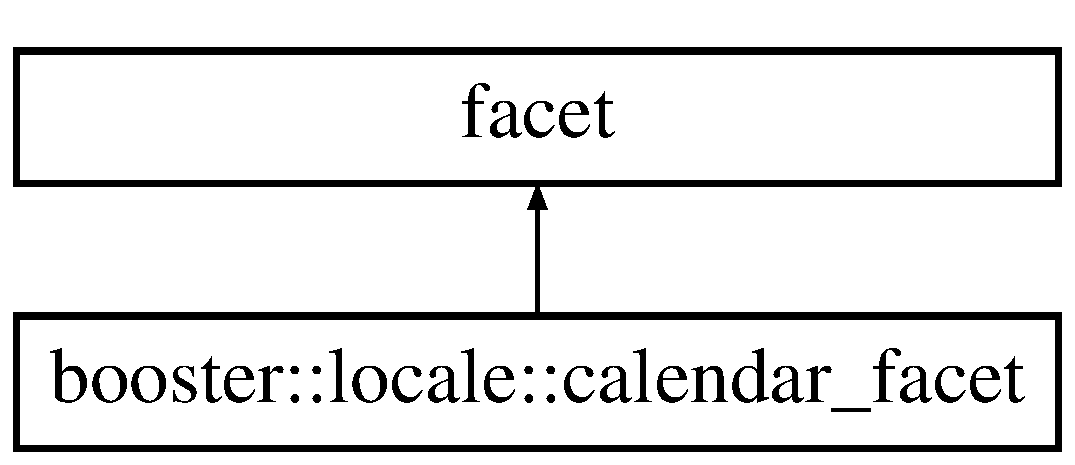
\includegraphics[height=2.000000cm]{classbooster_1_1locale_1_1calendar__facet}
\end{center}
\end{figure}
\subsection*{Public Member Functions}
\begin{DoxyCompactItemize}
\item 
{\bf calendar\+\_\+facet} (size\+\_\+t refs=0)
\item 
virtual {\bf abstract\+\_\+calendar} $\ast$ {\bf create\+\_\+calendar} () const =0
\end{DoxyCompactItemize}
\subsection*{Static Public Attributes}
\begin{DoxyCompactItemize}
\item 
static std\+::locale\+::id {\bf id}
\end{DoxyCompactItemize}


\subsection{Detailed Description}
the facet that generates calendar for specific locale 

\subsection{Constructor \& Destructor Documentation}
\index{booster\+::locale\+::calendar\+\_\+facet@{booster\+::locale\+::calendar\+\_\+facet}!calendar\+\_\+facet@{calendar\+\_\+facet}}
\index{calendar\+\_\+facet@{calendar\+\_\+facet}!booster\+::locale\+::calendar\+\_\+facet@{booster\+::locale\+::calendar\+\_\+facet}}
\subsubsection[{calendar\+\_\+facet(size\+\_\+t refs=0)}]{\setlength{\rightskip}{0pt plus 5cm}booster\+::locale\+::calendar\+\_\+facet\+::calendar\+\_\+facet (
\begin{DoxyParamCaption}
\item[{size\+\_\+t}]{refs = {\ttfamily 0}}
\end{DoxyParamCaption}
)\hspace{0.3cm}{\ttfamily [inline]}}\label{classbooster_1_1locale_1_1calendar__facet_ad594306664590e3bf9175f31491975b8}
Basic constructor 

\subsection{Member Function Documentation}
\index{booster\+::locale\+::calendar\+\_\+facet@{booster\+::locale\+::calendar\+\_\+facet}!create\+\_\+calendar@{create\+\_\+calendar}}
\index{create\+\_\+calendar@{create\+\_\+calendar}!booster\+::locale\+::calendar\+\_\+facet@{booster\+::locale\+::calendar\+\_\+facet}}
\subsubsection[{create\+\_\+calendar() const =0}]{\setlength{\rightskip}{0pt plus 5cm}virtual {\bf abstract\+\_\+calendar}$\ast$ booster\+::locale\+::calendar\+\_\+facet\+::create\+\_\+calendar (
\begin{DoxyParamCaption}
{}
\end{DoxyParamCaption}
) const\hspace{0.3cm}{\ttfamily [pure virtual]}}\label{classbooster_1_1locale_1_1calendar__facet_a0b29c6a19fcddb5e263329fa6ac2be4b}
Create a new calendar that points to current point of time. 

\subsection{Member Data Documentation}
\index{booster\+::locale\+::calendar\+\_\+facet@{booster\+::locale\+::calendar\+\_\+facet}!id@{id}}
\index{id@{id}!booster\+::locale\+::calendar\+\_\+facet@{booster\+::locale\+::calendar\+\_\+facet}}
\subsubsection[{id}]{\setlength{\rightskip}{0pt plus 5cm}std\+::locale\+::id booster\+::locale\+::calendar\+\_\+facet\+::id\hspace{0.3cm}{\ttfamily [static]}}\label{classbooster_1_1locale_1_1calendar__facet_a0879444f636f6520c74e2abb4615f53f}
Locale id (needed to work with std\+::locale) 

The documentation for this class was generated from the following file\+:\begin{DoxyCompactItemize}
\item 
booster/locale/date\+\_\+time\+\_\+facet.\+h\end{DoxyCompactItemize}

\section{cppcms\+:\+:rpc\+:\+:call\+\_\+error Class Reference}
\label{classcppcms_1_1rpc_1_1call__error}\index{cppcms\+::rpc\+::call\+\_\+error@{cppcms\+::rpc\+::call\+\_\+error}}


The error thrown in case of bad call -\/ parameters mismatch or invalid request.  




{\ttfamily \#include $<$cppcms/rpc\+\_\+json.\+h$>$}

Inheritance diagram for cppcms\+:\+:rpc\+:\+:call\+\_\+error\+:\begin{figure}[H]
\begin{center}
\leavevmode
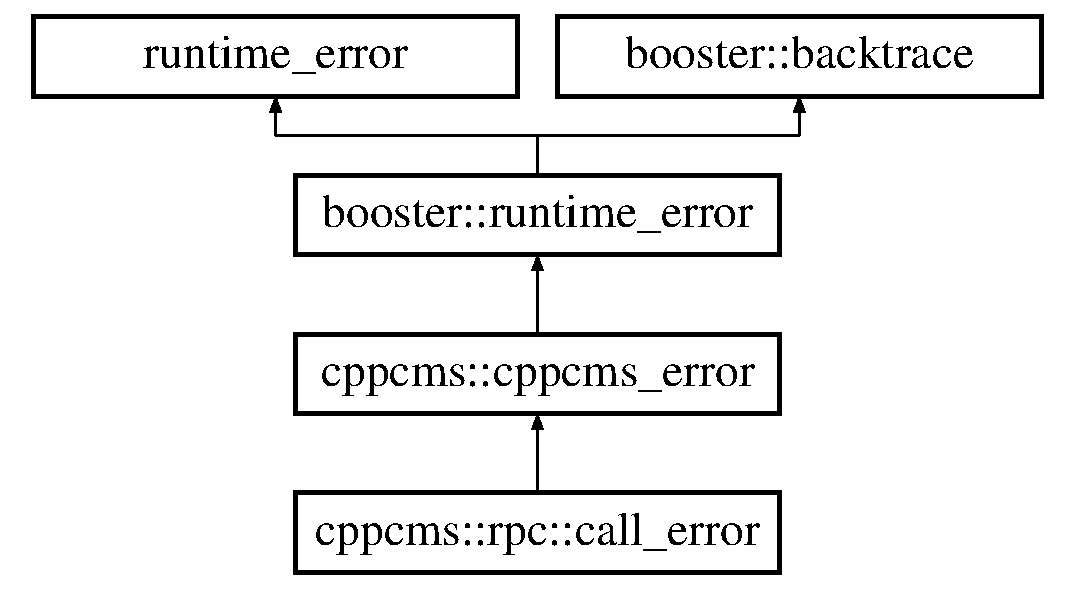
\includegraphics[height=4.000000cm]{classcppcms_1_1rpc_1_1call__error}
\end{center}
\end{figure}
\subsection*{Public Member Functions}
\begin{DoxyCompactItemize}
\item 
{\bf call\+\_\+error} (std\+::string const \&message)
\end{DoxyCompactItemize}
\subsection*{Additional Inherited Members}


\subsection{Detailed Description}
The error thrown in case of bad call -\/ parameters mismatch or invalid request. 

User should may throw it case of a error as invalid request inside the method. However return\+\_\+error() is preferred. 

\subsection{Constructor \& Destructor Documentation}
\index{cppcms\+::rpc\+::call\+\_\+error@{cppcms\+::rpc\+::call\+\_\+error}!call\+\_\+error@{call\+\_\+error}}
\index{call\+\_\+error@{call\+\_\+error}!cppcms\+::rpc\+::call\+\_\+error@{cppcms\+::rpc\+::call\+\_\+error}}
\subsubsection[{call\+\_\+error(std\+::string const \&message)}]{\setlength{\rightskip}{0pt plus 5cm}cppcms\+::rpc\+::call\+\_\+error\+::call\+\_\+error (
\begin{DoxyParamCaption}
\item[{std\+::string const \&}]{message}
\end{DoxyParamCaption}
)}\label{classcppcms_1_1rpc_1_1call__error_a8454f3491d79ffc078fe74fec70aa158}
Define error message 

The documentation for this class was generated from the following file\+:\begin{DoxyCompactItemize}
\item 
cppcms/rpc\+\_\+json.\+h\end{DoxyCompactItemize}

\section{booster\+:\+:callable$<$ Type $>$ Struct Template Reference}
\label{structbooster_1_1callable}\index{booster\+::callable$<$ Type $>$@{booster\+::callable$<$ Type $>$}}


The documentation for this struct was generated from the following file\+:\begin{DoxyCompactItemize}
\item 
booster/callback.\+h\end{DoxyCompactItemize}

\section{booster\+:\+:callable$<$ Result(Params...)$>$ Struct Template Reference}
\label{structbooster_1_1callable_3_01Result_07Params_8_8_8_08_4}\index{booster\+::callable$<$ Result(\+Params...)$>$@{booster\+::callable$<$ Result(\+Params...)$>$}}
Inheritance diagram for booster\+:\+:callable$<$ Result(Params...)$>$\+:\begin{figure}[H]
\begin{center}
\leavevmode
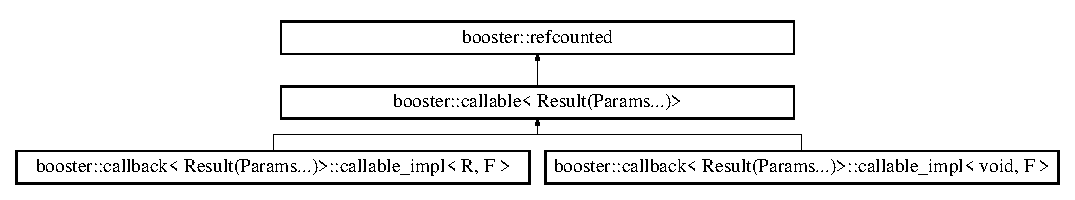
\includegraphics[height=2.245989cm]{structbooster_1_1callable_3_01Result_07Params_8_8_8_08_4}
\end{center}
\end{figure}
\subsection*{Public Member Functions}
\begin{DoxyCompactItemize}
\item 
virtual Result {\bfseries operator()} (Params...)=0\label{structbooster_1_1callable_3_01Result_07Params_8_8_8_08_4_abed5d6565425b2e15a67a4e0e40eede7}

\end{DoxyCompactItemize}


The documentation for this struct was generated from the following file\+:\begin{DoxyCompactItemize}
\item 
booster/callback.\+h\end{DoxyCompactItemize}

\section{booster\+:\+:callback$<$ Result(Params...)$>$\+:\+:callable\+\_\+impl$<$ R, F $>$ Struct Template Reference}
\label{structbooster_1_1callback_3_01Result_07Params_8_8_8_08_4_1_1callable__impl}\index{booster\+::callback$<$ Result(\+Params...)$>$\+::callable\+\_\+impl$<$ R, F $>$@{booster\+::callback$<$ Result(\+Params...)$>$\+::callable\+\_\+impl$<$ R, F $>$}}
Inheritance diagram for booster\+:\+:callback$<$ Result(Params...)$>$\+:\+:callable\+\_\+impl$<$ R, F $>$\+:\begin{figure}[H]
\begin{center}
\leavevmode
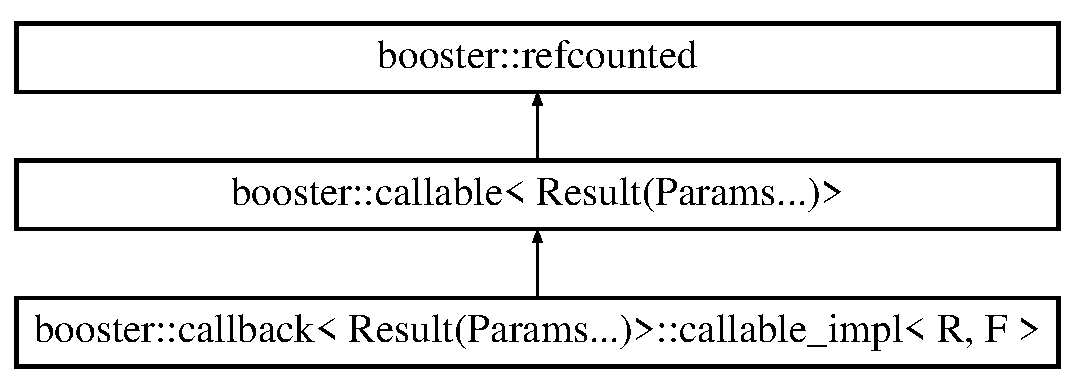
\includegraphics[height=3.000000cm]{structbooster_1_1callback_3_01Result_07Params_8_8_8_08_4_1_1callable__impl}
\end{center}
\end{figure}
\subsection*{Public Member Functions}
\begin{DoxyCompactItemize}
\item 
{\bfseries callable\+\_\+impl} (F f)\label{structbooster_1_1callback_3_01Result_07Params_8_8_8_08_4_1_1callable__impl_a4175590398e9a72e2eeda859e10001ae}

\item 
virtual R {\bfseries operator()} (Params...\+args)\label{structbooster_1_1callback_3_01Result_07Params_8_8_8_08_4_1_1callable__impl_ae1eb421b84a20c3135520be172caa246}

\end{DoxyCompactItemize}
\subsection*{Public Attributes}
\begin{DoxyCompactItemize}
\item 
F {\bfseries func}\label{structbooster_1_1callback_3_01Result_07Params_8_8_8_08_4_1_1callable__impl_a37c8cf1f67888504410df2628a8bb539}

\end{DoxyCompactItemize}


The documentation for this struct was generated from the following file\+:\begin{DoxyCompactItemize}
\item 
booster/callback.\+h\end{DoxyCompactItemize}

\section{booster\+:\+:callback$<$ Result(Params...)$>$\+:\+:callable\+\_\+impl$<$ void, F $>$ Struct Template Reference}
\label{structbooster_1_1callback_3_01Result_07Params_8_8_8_08_4_1_1callable__impl_3_01void_00_01F_01_4}\index{booster\+::callback$<$ Result(\+Params...)$>$\+::callable\+\_\+impl$<$ void, F $>$@{booster\+::callback$<$ Result(\+Params...)$>$\+::callable\+\_\+impl$<$ void, F $>$}}
Inheritance diagram for booster\+:\+:callback$<$ Result(Params...)$>$\+:\+:callable\+\_\+impl$<$ void, F $>$\+:\begin{figure}[H]
\begin{center}
\leavevmode
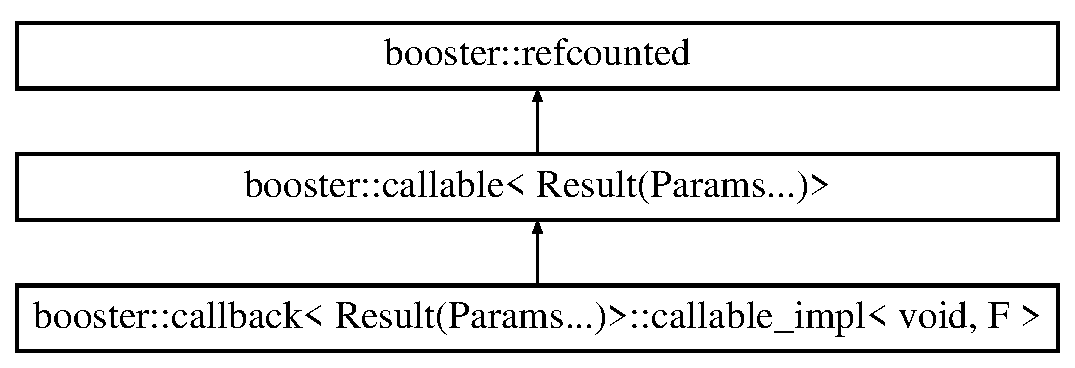
\includegraphics[height=3.000000cm]{structbooster_1_1callback_3_01Result_07Params_8_8_8_08_4_1_1callable__impl_3_01void_00_01F_01_4}
\end{center}
\end{figure}
\subsection*{Public Member Functions}
\begin{DoxyCompactItemize}
\item 
{\bfseries callable\+\_\+impl} (F f)\label{structbooster_1_1callback_3_01Result_07Params_8_8_8_08_4_1_1callable__impl_3_01void_00_01F_01_4_ab8647f4dfe07d3138926628ecd951f47}

\item 
virtual void {\bfseries operator()} (Params...\+args)\label{structbooster_1_1callback_3_01Result_07Params_8_8_8_08_4_1_1callable__impl_3_01void_00_01F_01_4_acf622b8a698f9ac9bdfd193f32f5e107}

\end{DoxyCompactItemize}
\subsection*{Public Attributes}
\begin{DoxyCompactItemize}
\item 
F {\bfseries func}\label{structbooster_1_1callback_3_01Result_07Params_8_8_8_08_4_1_1callable__impl_3_01void_00_01F_01_4_a1d9256439f3c5579ec5e379c81321e4b}

\end{DoxyCompactItemize}


The documentation for this struct was generated from the following file\+:\begin{DoxyCompactItemize}
\item 
booster/callback.\+h\end{DoxyCompactItemize}

\section{booster\+:\+:callback$<$ Type $>$ Class Template Reference}
\label{classbooster_1_1callback}\index{booster\+::callback$<$ Type $>$@{booster\+::callback$<$ Type $>$}}


The documentation for this class was generated from the following file\+:\begin{DoxyCompactItemize}
\item 
booster/callback.\+h\end{DoxyCompactItemize}

\section{booster\+:\+:callback$<$ Result(Params...)$>$ Class Template Reference}
\label{classbooster_1_1callback_3_01Result_07Params_8_8_8_08_4}\index{booster\+::callback$<$ Result(\+Params...)$>$@{booster\+::callback$<$ Result(\+Params...)$>$}}


This is Booster\textquotesingle{}s implementation of std\+::tr1\+::callback/booster\+::callback.  




{\ttfamily \#include $<$booster/booster/callback.\+h$>$}

\subsection*{Classes}
\begin{DoxyCompactItemize}
\item 
struct {\bf callable\+\_\+impl}
\item 
struct {\bf callable\+\_\+impl$<$ void, F $>$}
\end{DoxyCompactItemize}
\subsection*{Public Types}
\begin{DoxyCompactItemize}
\item 
typedef Result {\bfseries result\+\_\+type}\label{classbooster_1_1callback_3_01Result_07Params_8_8_8_08_4_ac2a710604dbf22edf06ccab4e8fffb20}

\item 
typedef {\bf callable}$<$ Result(Params...)$>$ {\bfseries callable\+\_\+type}\label{classbooster_1_1callback_3_01Result_07Params_8_8_8_08_4_a70891f5d4a2296ace31ba2ca697ff932}

\item 
typedef {\bf intrusive\+\_\+ptr}$<$ {\bf callable\+\_\+type} $>$ {\bf pointer\+\_\+type}
\end{DoxyCompactItemize}
\subsection*{Public Member Functions}
\begin{DoxyCompactItemize}
\item 
{\bf callback} ()
\item 
{\footnotesize template$<$typename Call $>$ }\\{\bfseries callback} ({\bf intrusive\+\_\+ptr}$<$ Call $>$ c)\label{classbooster_1_1callback_3_01Result_07Params_8_8_8_08_4_a1413b20da6de3bebc7b0e5bc67f85632}

\item 
{\footnotesize template$<$typename Call $>$ }\\{\bfseries callback} (std\+::unique\+\_\+ptr$<$ Call $>$ ptr)\label{classbooster_1_1callback_3_01Result_07Params_8_8_8_08_4_ae3f8d6b0da468a736007359a5ee962ab}

\item 
{\footnotesize template$<$typename Call $>$ }\\{\bf callback} const \& {\bfseries operator=} ({\bf intrusive\+\_\+ptr}$<$ Call $>$ c)\label{classbooster_1_1callback_3_01Result_07Params_8_8_8_08_4_a942fc8a4c93a7c737835656fba58af6e}

\item 
{\footnotesize template$<$typename Call $>$ }\\{\bf callback} const \& {\bfseries operator=} (std\+::unique\+\_\+ptr$<$ Call $>$ c)\label{classbooster_1_1callback_3_01Result_07Params_8_8_8_08_4_a6bc4f30c9229bc3f390bbd79760a0d1c}

\item 
{\footnotesize template$<$typename F $>$ }\\{\bfseries callback} (F func)\label{classbooster_1_1callback_3_01Result_07Params_8_8_8_08_4_ac222ac49bf4e166e80e5378ebd4989aa}

\item 
{\bfseries callback} ({\bf callback} const \&other)\label{classbooster_1_1callback_3_01Result_07Params_8_8_8_08_4_a7652f092533298870d5f714005c5a0a2}

\item 
{\bfseries callback} ({\bf callback} \&\&other)\label{classbooster_1_1callback_3_01Result_07Params_8_8_8_08_4_ab869fe0c37684c354a252bd5b96f5b93}

\item 
{\footnotesize template$<$typename F $>$ }\\{\bf callback} const \& {\bfseries operator=} (F func)\label{classbooster_1_1callback_3_01Result_07Params_8_8_8_08_4_af15f7842f37bbd07bb6bbc25968d5501}

\item 
{\bf callback} \& {\bfseries operator=} ({\bf callback} \&\&other)\label{classbooster_1_1callback_3_01Result_07Params_8_8_8_08_4_a64a1e37a0bae921b2018b4f787d6698c}

\item 
{\bf callback} const \& {\bfseries operator=} ({\bf callback} const \&other)\label{classbooster_1_1callback_3_01Result_07Params_8_8_8_08_4_a5647e0e4491a0fd4120aa47e49589b70}

\item 
Result {\bfseries operator()} (Params...\+args) const \label{classbooster_1_1callback_3_01Result_07Params_8_8_8_08_4_ab374a6e20bec5d43829fa308ed439083}

\item 
bool {\bf empty} () const 
\item 
{\bf operator bool} () const 
\item 
void {\bfseries swap} ({\bf callback} \&other)\label{classbooster_1_1callback_3_01Result_07Params_8_8_8_08_4_a900e3aae42c5d48f1b4ef97d529118d7}

\item 
{\bf pointer\+\_\+type} const \& {\bfseries get\+\_\+pointer} () const \label{classbooster_1_1callback_3_01Result_07Params_8_8_8_08_4_acb80da60f48b1352a245bb60606fe2bb}

\item 
{\bf pointer\+\_\+type} \& {\bfseries get\+\_\+pointer} ()\label{classbooster_1_1callback_3_01Result_07Params_8_8_8_08_4_aec7cf6efabd0dc69615c40ecdd07703c}

\end{DoxyCompactItemize}


\subsection{Detailed Description}
\subsubsection*{template$<$typename Result, typename... Params$>$\\*
class booster\+::callback$<$ Result(\+Params...)$>$}

This is Booster\textquotesingle{}s implementation of std\+::tr1\+::callback/booster\+::callback. 

This callback is created from generic object that can be \char`\"{}called\char`\"{} i.\+e. a class with operator() or callback pointer that has same signature as the callback.

See\+: {\tt http\+://www.\+boost.\+org/doc/html/function.\+html}

Notes\+:


\begin{DoxyItemize}
\item this code is not taken from Boost and has slightly different interface.
\item as most of compilers do not support Variadic templates yet, this class is explicitly specialized for Params of size 0 to 8. So maximal amout of parameters that can be used is 8. 
\end{DoxyItemize}

\subsection{Member Typedef Documentation}
\index{booster\+::callback$<$ Result(\+Params...)$>$@{booster\+::callback$<$ Result(\+Params...)$>$}!pointer\+\_\+type@{pointer\+\_\+type}}
\index{pointer\+\_\+type@{pointer\+\_\+type}!booster\+::callback$<$ Result(\+Params...)$>$@{booster\+::callback$<$ Result(\+Params...)$>$}}
\subsubsection[{pointer\+\_\+type}]{\setlength{\rightskip}{0pt plus 5cm}template$<$typename Result , typename... Params$>$ typedef {\bf intrusive\+\_\+ptr}$<${\bf callable\+\_\+type}$>$ {\bf booster\+::callback}$<$ Result(Params...)$>$\+::{\bf pointer\+\_\+type}}\label{classbooster_1_1callback_3_01Result_07Params_8_8_8_08_4_a014c509ca6bb999aff7512804cfba635}
Pointer to callable object

\doxyref{New in Cpp\+C\+MS 1.\+2}{p.}{v1_2} 

\subsection{Constructor \& Destructor Documentation}
\index{booster\+::callback$<$ Result(\+Params...)$>$@{booster\+::callback$<$ Result(\+Params...)$>$}!callback@{callback}}
\index{callback@{callback}!booster\+::callback$<$ Result(\+Params...)$>$@{booster\+::callback$<$ Result(\+Params...)$>$}}
\subsubsection[{callback()}]{\setlength{\rightskip}{0pt plus 5cm}template$<$typename Result , typename... Params$>$ {\bf booster\+::callback}$<$ Result(Params...)$>$\+::{\bf callback} (
\begin{DoxyParamCaption}
{}
\end{DoxyParamCaption}
)\hspace{0.3cm}{\ttfamily [inline]}}\label{classbooster_1_1callback_3_01Result_07Params_8_8_8_08_4_a53778f82188d5ce241ac777e4b67830c}
Default constructor, creates an empty callbacks 

\subsection{Member Function Documentation}
\index{booster\+::callback$<$ Result(\+Params...)$>$@{booster\+::callback$<$ Result(\+Params...)$>$}!empty@{empty}}
\index{empty@{empty}!booster\+::callback$<$ Result(\+Params...)$>$@{booster\+::callback$<$ Result(\+Params...)$>$}}
\subsubsection[{empty() const }]{\setlength{\rightskip}{0pt plus 5cm}template$<$typename Result , typename... Params$>$ bool {\bf booster\+::callback}$<$ Result(Params...)$>$\+::empty (
\begin{DoxyParamCaption}
{}
\end{DoxyParamCaption}
) const\hspace{0.3cm}{\ttfamily [inline]}}\label{classbooster_1_1callback_3_01Result_07Params_8_8_8_08_4_a602d1091621c7942529205fe562142c2}
Return true if the callback is empty \index{booster\+::callback$<$ Result(\+Params...)$>$@{booster\+::callback$<$ Result(\+Params...)$>$}!operator bool@{operator bool}}
\index{operator bool@{operator bool}!booster\+::callback$<$ Result(\+Params...)$>$@{booster\+::callback$<$ Result(\+Params...)$>$}}
\subsubsection[{operator bool() const }]{\setlength{\rightskip}{0pt plus 5cm}template$<$typename Result , typename... Params$>$ {\bf booster\+::callback}$<$ Result(Params...)$>$\+::operator bool (
\begin{DoxyParamCaption}
{}
\end{DoxyParamCaption}
) const\hspace{0.3cm}{\ttfamily [inline]}}\label{classbooster_1_1callback_3_01Result_07Params_8_8_8_08_4_a1302b4d05c5e9df392664dd7ff5ae437}
Returns true if the callback is not empty 

The documentation for this class was generated from the following file\+:\begin{DoxyCompactItemize}
\item 
booster/callback.\+h\end{DoxyCompactItemize}

\section{booster\+:\+:aio\+:\+:aio\+\_\+error\+:\+:category Class Reference}
\label{classbooster_1_1aio_1_1aio__error_1_1category}\index{booster\+::aio\+::aio\+\_\+error\+::category@{booster\+::aio\+::aio\+\_\+error\+::category}}


{\ttfamily \#include $<$booster/booster/aio/aio\+\_\+category.\+h$>$}

Inheritance diagram for booster\+:\+:aio\+:\+:aio\+\_\+error\+:\+:category\+:\begin{figure}[H]
\begin{center}
\leavevmode
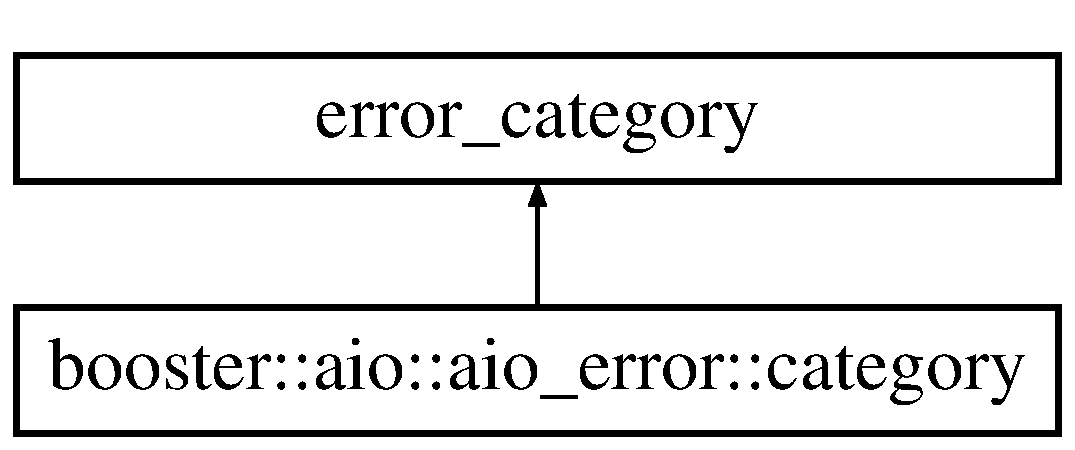
\includegraphics[height=2.000000cm]{classbooster_1_1aio_1_1aio__error_1_1category}
\end{center}
\end{figure}
\subsection*{Public Member Functions}
\begin{DoxyCompactItemize}
\item 
{\bfseries category} ({\bf category} \&\&)\label{classbooster_1_1aio_1_1aio__error_1_1category_ae68e35aeedf7de3cdd17d65924245f42}

\item 
virtual char const $\ast$ {\bf name} () const noexcept\label{classbooster_1_1aio_1_1aio__error_1_1category_a1842cfbd1311d16dab0fcd57c3053a41}

\begin{DoxyCompactList}\small\item\em Get category name. \end{DoxyCompactList}\item 
virtual std\+::string {\bf message} (int cat) const \label{classbooster_1_1aio_1_1aio__error_1_1category_a64ecec92aeb8448331377385353abe39}

\begin{DoxyCompactList}\small\item\em Get message from code. \end{DoxyCompactList}\end{DoxyCompactItemize}


\subsection{Detailed Description}
Error category for \doxyref{booster\+::aio}{p.}{namespacebooster_1_1aio} objects 

The documentation for this class was generated from the following file\+:\begin{DoxyCompactItemize}
\item 
booster/aio/aio\+\_\+category.\+h\end{DoxyCompactItemize}

\section{cppcms\+:\+:crypto\+:\+:cbc Class Reference}
\label{classcppcms_1_1crypto_1_1cbc}\index{cppcms\+::crypto\+::cbc@{cppcms\+::crypto\+::cbc}}


Cipher-\/block chaining encryption and decryption cryptographic service.  




{\ttfamily \#include $<$cppcms/crypto.\+h$>$}

Inheritance diagram for cppcms\+:\+:crypto\+:\+:cbc\+:\begin{figure}[H]
\begin{center}
\leavevmode
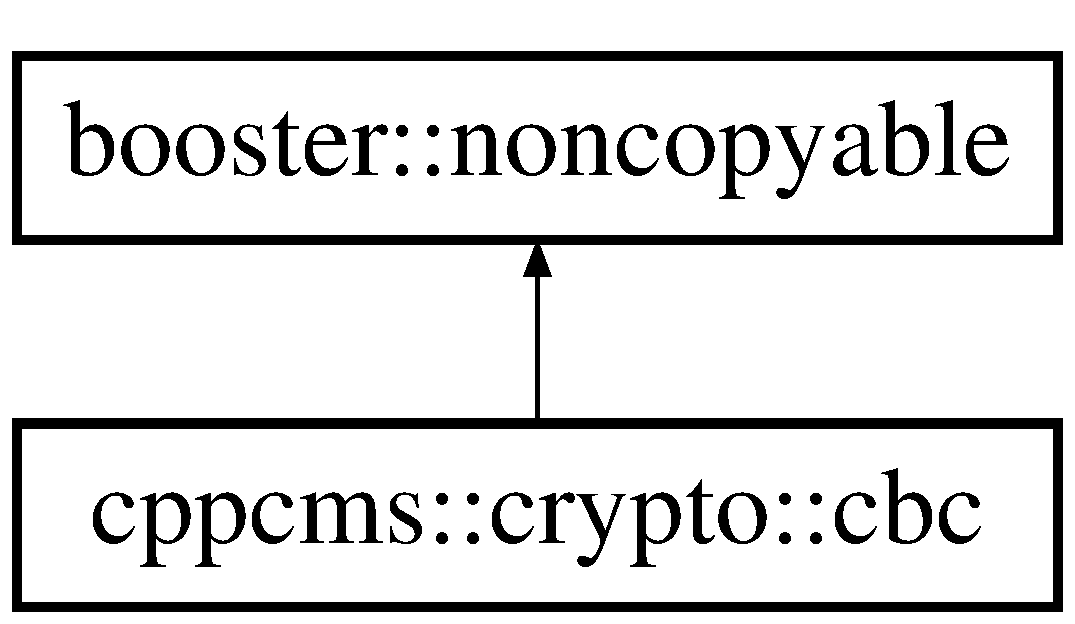
\includegraphics[height=2.000000cm]{classcppcms_1_1crypto_1_1cbc}
\end{center}
\end{figure}
\subsection*{Public Types}
\begin{DoxyCompactItemize}
\item 
enum {\bf cbc\+\_\+type} \{ {\bf aes128} = 0, 
{\bf aes192} = 1, 
{\bf aes256} = 2
 \}
\end{DoxyCompactItemize}
\subsection*{Public Member Functions}
\begin{DoxyCompactItemize}
\item 
virtual unsigned {\bf block\+\_\+size} () const =0
\item 
virtual unsigned {\bf key\+\_\+size} () const =0
\item 
virtual void {\bf set\+\_\+key} ({\bf key} const \&)=0
\item 
virtual void {\bf set\+\_\+iv} (void const $\ast$ptr, size\+\_\+t size)=0
\item 
virtual void {\bf set\+\_\+nonce\+\_\+iv} ()=0
\item 
virtual void {\bf encrypt} (void const $\ast$in, void $\ast$out, unsigned len)=0
\item 
virtual void {\bf decrypt} (void const $\ast$in, void $\ast$out, unsigned len)=0
\end{DoxyCompactItemize}
\subsection*{Static Public Member Functions}
\begin{DoxyCompactItemize}
\item 
static std\+::unique\+\_\+ptr$<$ {\bf cbc} $>$ {\bf create} ({\bf cbc\+\_\+type} type)
\item 
static std\+::unique\+\_\+ptr$<$ {\bf cbc} $>$ {\bf create} (std\+::string const \&name)
\end{DoxyCompactItemize}


\subsection{Detailed Description}
Cipher-\/block chaining encryption and decryption cryptographic service. 

\begin{DoxyNote}{Note}
In order to use it, you {\bfseries must} compile Cpp\+C\+MS with Open\+S\+SL (libcrypto) or G\+N\+U-\/\+T\+LS (libgcrypt) library. 
\end{DoxyNote}


\subsection{Member Enumeration Documentation}
\index{cppcms\+::crypto\+::cbc@{cppcms\+::crypto\+::cbc}!cbc\+\_\+type@{cbc\+\_\+type}}
\index{cbc\+\_\+type@{cbc\+\_\+type}!cppcms\+::crypto\+::cbc@{cppcms\+::crypto\+::cbc}}
\subsubsection[{cbc\+\_\+type}]{\setlength{\rightskip}{0pt plus 5cm}enum {\bf cppcms\+::crypto\+::cbc\+::cbc\+\_\+type}}\label{classcppcms_1_1crypto_1_1cbc_a6a4d426a4322e3fe8f3596e60f2933f1}
C\+BC encryption type \begin{Desc}
\item[Enumerator]\par
\begin{description}
\index{aes128@{aes128}!cppcms\+::crypto\+::cbc@{cppcms\+::crypto\+::cbc}}\index{cppcms\+::crypto\+::cbc@{cppcms\+::crypto\+::cbc}!aes128@{aes128}}\item[{\em 
aes128\label{classcppcms_1_1crypto_1_1cbc_a6a4d426a4322e3fe8f3596e60f2933f1ad8d07a81acc5674e21906667ff004244}
}]A\+E\+S-\/128. \index{aes192@{aes192}!cppcms\+::crypto\+::cbc@{cppcms\+::crypto\+::cbc}}\index{cppcms\+::crypto\+::cbc@{cppcms\+::crypto\+::cbc}!aes192@{aes192}}\item[{\em 
aes192\label{classcppcms_1_1crypto_1_1cbc_a6a4d426a4322e3fe8f3596e60f2933f1a509f84b5870914ba7ffe3bb2a5d077bf}
}]A\+E\+S-\/192. \index{aes256@{aes256}!cppcms\+::crypto\+::cbc@{cppcms\+::crypto\+::cbc}}\index{cppcms\+::crypto\+::cbc@{cppcms\+::crypto\+::cbc}!aes256@{aes256}}\item[{\em 
aes256\label{classcppcms_1_1crypto_1_1cbc_a6a4d426a4322e3fe8f3596e60f2933f1ab6206d852671df0c9bf1f01b4c972715}
}]A\+E\+S-\/256. \end{description}
\end{Desc}


\subsection{Member Function Documentation}
\index{cppcms\+::crypto\+::cbc@{cppcms\+::crypto\+::cbc}!block\+\_\+size@{block\+\_\+size}}
\index{block\+\_\+size@{block\+\_\+size}!cppcms\+::crypto\+::cbc@{cppcms\+::crypto\+::cbc}}
\subsubsection[{block\+\_\+size() const =0}]{\setlength{\rightskip}{0pt plus 5cm}virtual unsigned cppcms\+::crypto\+::cbc\+::block\+\_\+size (
\begin{DoxyParamCaption}
{}
\end{DoxyParamCaption}
) const\hspace{0.3cm}{\ttfamily [pure virtual]}}\label{classcppcms_1_1crypto_1_1cbc_a97247cdede2da296b0e92a0cfe73dad2}
Get the size of the block C\+BC works on \index{cppcms\+::crypto\+::cbc@{cppcms\+::crypto\+::cbc}!create@{create}}
\index{create@{create}!cppcms\+::crypto\+::cbc@{cppcms\+::crypto\+::cbc}}
\subsubsection[{create(cbc\+\_\+type type)}]{\setlength{\rightskip}{0pt plus 5cm}static std\+::unique\+\_\+ptr$<${\bf cbc}$>$ cppcms\+::crypto\+::cbc\+::create (
\begin{DoxyParamCaption}
\item[{{\bf cbc\+\_\+type}}]{type}
\end{DoxyParamCaption}
)\hspace{0.3cm}{\ttfamily [static]}}\label{classcppcms_1_1crypto_1_1cbc_aed495f26bb2203639a816b83428c4df7}
Create a new cbc object that performs encryption using {\itshape type} method.

If the encryption method is not supported returns an empty pointer! \index{cppcms\+::crypto\+::cbc@{cppcms\+::crypto\+::cbc}!create@{create}}
\index{create@{create}!cppcms\+::crypto\+::cbc@{cppcms\+::crypto\+::cbc}}
\subsubsection[{create(std\+::string const \&name)}]{\setlength{\rightskip}{0pt plus 5cm}static std\+::unique\+\_\+ptr$<${\bf cbc}$>$ cppcms\+::crypto\+::cbc\+::create (
\begin{DoxyParamCaption}
\item[{std\+::string const \&}]{name}
\end{DoxyParamCaption}
)\hspace{0.3cm}{\ttfamily [static]}}\label{classcppcms_1_1crypto_1_1cbc_ac6a52828e66a2cca5fee03e6fce22cb0}
Create a new cbc object that performs encryption using algorithm {\itshape name} 

If the encryption method is not supported returns an empty pointer!

Currently supported aes128, aes192, aes256, with names \char`\"{}aes\char`\"{} = \char`\"{}aes-\/128\char`\"{} = \char`\"{}aes128\char`\"{} , \char`\"{}aes-\/192\char`\"{} \char`\"{}aes192\char`\"{}, \char`\"{}aes-\/256\char`\"{} = \char`\"{}aes256\char`\"{}. They require Cpp\+C\+MS to be compiled with Open\+S\+SL or G\+N\+U-\/\+T\+LS library \index{cppcms\+::crypto\+::cbc@{cppcms\+::crypto\+::cbc}!decrypt@{decrypt}}
\index{decrypt@{decrypt}!cppcms\+::crypto\+::cbc@{cppcms\+::crypto\+::cbc}}
\subsubsection[{decrypt(void const $\ast$in, void $\ast$out, unsigned len)=0}]{\setlength{\rightskip}{0pt plus 5cm}virtual void cppcms\+::crypto\+::cbc\+::decrypt (
\begin{DoxyParamCaption}
\item[{void const $\ast$}]{in, }
\item[{void $\ast$}]{out, }
\item[{unsigned}]{len}
\end{DoxyParamCaption}
)\hspace{0.3cm}{\ttfamily [pure virtual]}}\label{classcppcms_1_1crypto_1_1cbc_a7e54bd18f956d72b84c53b96e9f99538}
Decrypt the data {\itshape in} to {\itshape out} of size {\itshape len}. {\itshape len} should be multiple of \doxyref{block\+\_\+size()}{p.}{classcppcms_1_1crypto_1_1cbc_a97247cdede2da296b0e92a0cfe73dad2} \index{cppcms\+::crypto\+::cbc@{cppcms\+::crypto\+::cbc}!encrypt@{encrypt}}
\index{encrypt@{encrypt}!cppcms\+::crypto\+::cbc@{cppcms\+::crypto\+::cbc}}
\subsubsection[{encrypt(void const $\ast$in, void $\ast$out, unsigned len)=0}]{\setlength{\rightskip}{0pt plus 5cm}virtual void cppcms\+::crypto\+::cbc\+::encrypt (
\begin{DoxyParamCaption}
\item[{void const $\ast$}]{in, }
\item[{void $\ast$}]{out, }
\item[{unsigned}]{len}
\end{DoxyParamCaption}
)\hspace{0.3cm}{\ttfamily [pure virtual]}}\label{classcppcms_1_1crypto_1_1cbc_a7f2131e5822dc997b9833f7880733c5a}
Encrypt the data {\itshape in} to {\itshape out} of size {\itshape len}. {\itshape len} should be multiple of \doxyref{block\+\_\+size()}{p.}{classcppcms_1_1crypto_1_1cbc_a97247cdede2da296b0e92a0cfe73dad2} \index{cppcms\+::crypto\+::cbc@{cppcms\+::crypto\+::cbc}!key\+\_\+size@{key\+\_\+size}}
\index{key\+\_\+size@{key\+\_\+size}!cppcms\+::crypto\+::cbc@{cppcms\+::crypto\+::cbc}}
\subsubsection[{key\+\_\+size() const =0}]{\setlength{\rightskip}{0pt plus 5cm}virtual unsigned cppcms\+::crypto\+::cbc\+::key\+\_\+size (
\begin{DoxyParamCaption}
{}
\end{DoxyParamCaption}
) const\hspace{0.3cm}{\ttfamily [pure virtual]}}\label{classcppcms_1_1crypto_1_1cbc_a6dc620ac7b8ba0c80b8b96a701584bed}
Get the required key size in bytes \index{cppcms\+::crypto\+::cbc@{cppcms\+::crypto\+::cbc}!set\+\_\+iv@{set\+\_\+iv}}
\index{set\+\_\+iv@{set\+\_\+iv}!cppcms\+::crypto\+::cbc@{cppcms\+::crypto\+::cbc}}
\subsubsection[{set\+\_\+iv(void const $\ast$ptr, size\+\_\+t size)=0}]{\setlength{\rightskip}{0pt plus 5cm}virtual void cppcms\+::crypto\+::cbc\+::set\+\_\+iv (
\begin{DoxyParamCaption}
\item[{void const $\ast$}]{ptr, }
\item[{size\+\_\+t}]{size}
\end{DoxyParamCaption}
)\hspace{0.3cm}{\ttfamily [pure virtual]}}\label{classcppcms_1_1crypto_1_1cbc_ad8f668cb42c5735d4d735c8a48bbeeae}
Set initial vector value, size should be equal to \doxyref{block\+\_\+size()}{p.}{classcppcms_1_1crypto_1_1cbc_a97247cdede2da296b0e92a0cfe73dad2} \index{cppcms\+::crypto\+::cbc@{cppcms\+::crypto\+::cbc}!set\+\_\+key@{set\+\_\+key}}
\index{set\+\_\+key@{set\+\_\+key}!cppcms\+::crypto\+::cbc@{cppcms\+::crypto\+::cbc}}
\subsubsection[{set\+\_\+key(key const \&)=0}]{\setlength{\rightskip}{0pt plus 5cm}virtual void cppcms\+::crypto\+::cbc\+::set\+\_\+key (
\begin{DoxyParamCaption}
\item[{{\bf key} const \&}]{}
\end{DoxyParamCaption}
)\hspace{0.3cm}{\ttfamily [pure virtual]}}\label{classcppcms_1_1crypto_1_1cbc_a2a742877fcae62664e33a18083870a7d}
Set the key value \index{cppcms\+::crypto\+::cbc@{cppcms\+::crypto\+::cbc}!set\+\_\+nonce\+\_\+iv@{set\+\_\+nonce\+\_\+iv}}
\index{set\+\_\+nonce\+\_\+iv@{set\+\_\+nonce\+\_\+iv}!cppcms\+::crypto\+::cbc@{cppcms\+::crypto\+::cbc}}
\subsubsection[{set\+\_\+nonce\+\_\+iv()=0}]{\setlength{\rightskip}{0pt plus 5cm}virtual void cppcms\+::crypto\+::cbc\+::set\+\_\+nonce\+\_\+iv (
\begin{DoxyParamCaption}
{}
\end{DoxyParamCaption}
)\hspace{0.3cm}{\ttfamily [pure virtual]}}\label{classcppcms_1_1crypto_1_1cbc_a6c3435793b136c8797a3a9ca75746aee}
Set randomly created initial vector value 

The documentation for this class was generated from the following file\+:\begin{DoxyCompactItemize}
\item 
cppcms/crypto.\+h\end{DoxyCompactItemize}

\section{cppcms\+:\+:widgets\+:\+:checkbox Class Reference}
\label{classcppcms_1_1widgets_1_1checkbox}\index{cppcms\+::widgets\+::checkbox@{cppcms\+::widgets\+::checkbox}}


This class represent an H\+T\+ML checkbox input element.  




{\ttfamily \#include $<$cppcms/form.\+h$>$}

Inheritance diagram for cppcms\+:\+:widgets\+:\+:checkbox\+:\begin{figure}[H]
\begin{center}
\leavevmode
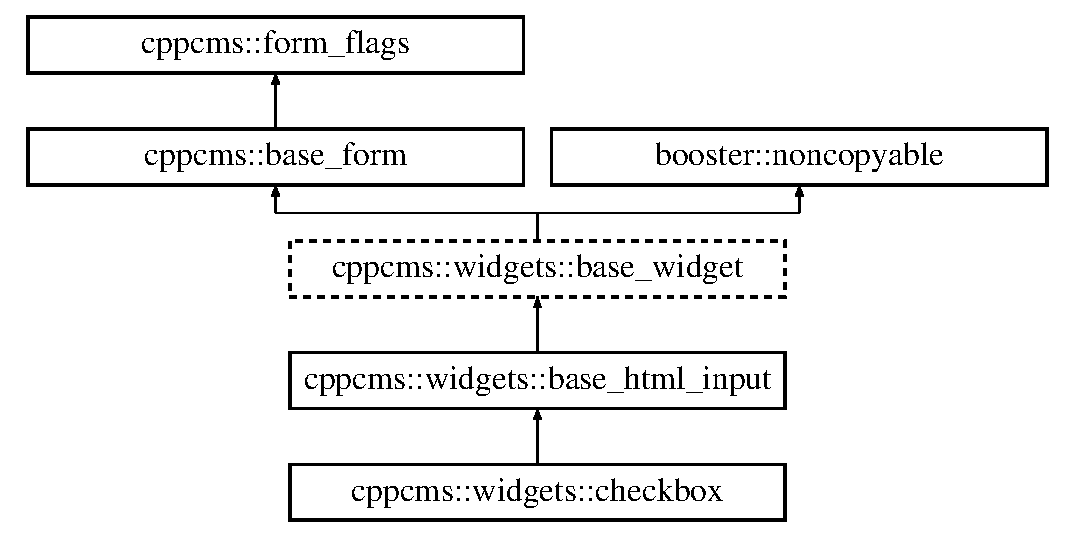
\includegraphics[height=5.000000cm]{classcppcms_1_1widgets_1_1checkbox}
\end{center}
\end{figure}
\subsection*{Public Member Functions}
\begin{DoxyCompactItemize}
\item 
{\bf checkbox} (std\+::string const \&type)
\item 
{\bf checkbox} ()
\item 
bool {\bf value} ()
\item 
void {\bf value} (bool is\+\_\+set)
\item 
std\+::string {\bf identification} ()
\item 
void {\bf identification} (std\+::string const \&)
\item 
virtual void {\bf render\+\_\+value} ({\bf form\+\_\+context} \&context)
\item 
virtual void {\bf load} ({\bf http\+::context} \&context)
\end{DoxyCompactItemize}
\subsection*{Additional Inherited Members}


\subsection{Detailed Description}
This class represent an H\+T\+ML checkbox input element. 

\subsection{Constructor \& Destructor Documentation}
\index{cppcms\+::widgets\+::checkbox@{cppcms\+::widgets\+::checkbox}!checkbox@{checkbox}}
\index{checkbox@{checkbox}!cppcms\+::widgets\+::checkbox@{cppcms\+::widgets\+::checkbox}}
\subsubsection[{checkbox(std\+::string const \&type)}]{\setlength{\rightskip}{0pt plus 5cm}cppcms\+::widgets\+::checkbox\+::checkbox (
\begin{DoxyParamCaption}
\item[{std\+::string const \&}]{type}
\end{DoxyParamCaption}
)}\label{classcppcms_1_1widgets_1_1checkbox_ab64c3216029dba87860c7fdd04ced47d}
The constructor that allows you to specify {\ttfamily type} H\+T\+ML attribute. It is passed to the constructor of the \doxyref{base\+\_\+html\+\_\+input}{p.}{classcppcms_1_1widgets_1_1base__html__input} class. \index{cppcms\+::widgets\+::checkbox@{cppcms\+::widgets\+::checkbox}!checkbox@{checkbox}}
\index{checkbox@{checkbox}!cppcms\+::widgets\+::checkbox@{cppcms\+::widgets\+::checkbox}}
\subsubsection[{checkbox()}]{\setlength{\rightskip}{0pt plus 5cm}cppcms\+::widgets\+::checkbox\+::checkbox (
\begin{DoxyParamCaption}
{}
\end{DoxyParamCaption}
)}\label{classcppcms_1_1widgets_1_1checkbox_accaaae0613a6f1b77d3e15e96544c1c2}
Default constructor. 

\subsection{Member Function Documentation}
\index{cppcms\+::widgets\+::checkbox@{cppcms\+::widgets\+::checkbox}!identification@{identification}}
\index{identification@{identification}!cppcms\+::widgets\+::checkbox@{cppcms\+::widgets\+::checkbox}}
\subsubsection[{identification()}]{\setlength{\rightskip}{0pt plus 5cm}std\+::string cppcms\+::widgets\+::checkbox\+::identification (
\begin{DoxyParamCaption}
{}
\end{DoxyParamCaption}
)}\label{classcppcms_1_1widgets_1_1checkbox_a7684910e7839280e2fa384344d17b3ef}
Get the unique identification string of the checkbox. \index{cppcms\+::widgets\+::checkbox@{cppcms\+::widgets\+::checkbox}!identification@{identification}}
\index{identification@{identification}!cppcms\+::widgets\+::checkbox@{cppcms\+::widgets\+::checkbox}}
\subsubsection[{identification(std\+::string const \&)}]{\setlength{\rightskip}{0pt plus 5cm}void cppcms\+::widgets\+::checkbox\+::identification (
\begin{DoxyParamCaption}
\item[{std\+::string const \&}]{}
\end{DoxyParamCaption}
)}\label{classcppcms_1_1widgets_1_1checkbox_ad89f0192be96890cc767a0f6f77fa000}
Set the unique identification string of the checkbox. It is useful when you want to have many options with the same name. \index{cppcms\+::widgets\+::checkbox@{cppcms\+::widgets\+::checkbox}!load@{load}}
\index{load@{load}!cppcms\+::widgets\+::checkbox@{cppcms\+::widgets\+::checkbox}}
\subsubsection[{load(http\+::context \&context)}]{\setlength{\rightskip}{0pt plus 5cm}virtual void cppcms\+::widgets\+::checkbox\+::load (
\begin{DoxyParamCaption}
\item[{{\bf http\+::context} \&}]{context}
\end{DoxyParamCaption}
)\hspace{0.3cm}{\ttfamily [virtual]}}\label{classcppcms_1_1widgets_1_1checkbox_a07910eeb823fe4ffd4e32fb8c2d0dc54}
Load the form information from the provided {\tt http\+::context} {\itshape context}. A user can call this function to load all information from the raw P\+O\+S\+T/\+G\+ET data into the internal widget representation. 

Implements {\bf cppcms\+::base\+\_\+form} \doxyref{}{p.}{classcppcms_1_1base__form_a5f9c5bbfba18076e898ec95827656bc1}.

\index{cppcms\+::widgets\+::checkbox@{cppcms\+::widgets\+::checkbox}!render\+\_\+value@{render\+\_\+value}}
\index{render\+\_\+value@{render\+\_\+value}!cppcms\+::widgets\+::checkbox@{cppcms\+::widgets\+::checkbox}}
\subsubsection[{render\+\_\+value(form\+\_\+context \&context)}]{\setlength{\rightskip}{0pt plus 5cm}virtual void cppcms\+::widgets\+::checkbox\+::render\+\_\+value (
\begin{DoxyParamCaption}
\item[{{\bf form\+\_\+context} \&}]{context}
\end{DoxyParamCaption}
)\hspace{0.3cm}{\ttfamily [virtual]}}\label{classcppcms_1_1widgets_1_1checkbox_aace5a796739449ade14f1d203f5d4b7d}
Write the actual value of the H\+T\+ML tag. Derived classes must implement this. 

Implements {\bf cppcms\+::widgets\+::base\+\_\+html\+\_\+input} \doxyref{}{p.}{classcppcms_1_1widgets_1_1base__html__input_afd2f99f7dd7b8ebe75e63f1f005068cb}.

\index{cppcms\+::widgets\+::checkbox@{cppcms\+::widgets\+::checkbox}!value@{value}}
\index{value@{value}!cppcms\+::widgets\+::checkbox@{cppcms\+::widgets\+::checkbox}}
\subsubsection[{value()}]{\setlength{\rightskip}{0pt plus 5cm}bool cppcms\+::widgets\+::checkbox\+::value (
\begin{DoxyParamCaption}
{}
\end{DoxyParamCaption}
)}\label{classcppcms_1_1widgets_1_1checkbox_a6e0e8154193ff93fb6a591263b815c04}
Return true if the checkbox was checked (selected). \index{cppcms\+::widgets\+::checkbox@{cppcms\+::widgets\+::checkbox}!value@{value}}
\index{value@{value}!cppcms\+::widgets\+::checkbox@{cppcms\+::widgets\+::checkbox}}
\subsubsection[{value(bool is\+\_\+set)}]{\setlength{\rightskip}{0pt plus 5cm}void cppcms\+::widgets\+::checkbox\+::value (
\begin{DoxyParamCaption}
\item[{bool}]{is\+\_\+set}
\end{DoxyParamCaption}
)}\label{classcppcms_1_1widgets_1_1checkbox_a6432de905e92a7ab263bcd72d532a5b4}
Set the state as {\itshape checked}. 

The documentation for this class was generated from the following file\+:\begin{DoxyCompactItemize}
\item 
cppcms/form.\+h\end{DoxyCompactItemize}

\section{booster\+:\+:clone\+\_\+ptr$<$ T $>$ Class Template Reference}
\label{classbooster_1_1clone__ptr}\index{booster\+::clone\+\_\+ptr$<$ T $>$@{booster\+::clone\+\_\+ptr$<$ T $>$}}


a smart pointer similar to std\+::unique\+\_\+ptr but it clones (by calling T\+::clone()) underlying object on copy instead of moving its ownership.  




{\ttfamily \#include $<$booster/booster/clone\+\_\+ptr.\+h$>$}

\subsection*{Public Member Functions}
\begin{DoxyCompactItemize}
\item 
{\bfseries clone\+\_\+ptr} (T $\ast$v)\label{classbooster_1_1clone__ptr_a25bbc5298997ae57cd05fe4c004ed974}

\item 
{\bfseries clone\+\_\+ptr} ({\bf clone\+\_\+ptr} \&\&other)\label{classbooster_1_1clone__ptr_a8b5d32a7b84efda3469a7f0fa281de54}

\item 
{\bf clone\+\_\+ptr} \& {\bfseries operator=} ({\bf clone\+\_\+ptr} \&\&other)\label{classbooster_1_1clone__ptr_af09ecb313352013a56992d4cee925abd}

\item 
{\bfseries clone\+\_\+ptr} ({\bf clone\+\_\+ptr} const \&other)\label{classbooster_1_1clone__ptr_a5e3b4ce855dc0b77f57879804230bbd5}

\item 
{\bf clone\+\_\+ptr} const \& {\bfseries operator=} ({\bf clone\+\_\+ptr} const \&other)\label{classbooster_1_1clone__ptr_ae7ade5f1b8410f2dfa56970d444d92bc}

\item 
T $\ast$ {\bfseries get} () const \label{classbooster_1_1clone__ptr_a2bc6c2017db9f1290e9fa378188d9d29}

\item 
T \& {\bfseries operator$\ast$} () const \label{classbooster_1_1clone__ptr_aee7534f5dcc06d0a2190c395f2fec2f6}

\item 
T $\ast$ {\bfseries operator-\/$>$} () const \label{classbooster_1_1clone__ptr_aee5a76d527f1901f95fdeb7180d3c6ce}

\item 
T $\ast$ {\bfseries release} ()\label{classbooster_1_1clone__ptr_a17c074b003bfc15b5c89d09b0145bcc6}

\item 
void {\bfseries reset} (T $\ast$p=0)\label{classbooster_1_1clone__ptr_a281dba30ac967d1f69d3ca866a3b66cd}

\item 
void {\bfseries swap} ({\bf clone\+\_\+ptr} \&other)\label{classbooster_1_1clone__ptr_ab0731bd2561a7c6a825b8010656f5e2c}

\end{DoxyCompactItemize}


\subsection{Detailed Description}
\subsubsection*{template$<$typename T$>$\\*
class booster\+::clone\+\_\+ptr$<$ T $>$}

a smart pointer similar to std\+::unique\+\_\+ptr but it clones (by calling T\+::clone()) underlying object on copy instead of moving its ownership. 

The documentation for this class was generated from the following file\+:\begin{DoxyCompactItemize}
\item 
booster/clone\+\_\+ptr.\+h\end{DoxyCompactItemize}

\section{booster\+:\+:locale\+:\+:collator$<$ Char\+Type $>$ Class Template Reference}
\label{classbooster_1_1locale_1_1collator}\index{booster\+::locale\+::collator$<$ Char\+Type $>$@{booster\+::locale\+::collator$<$ Char\+Type $>$}}


Collation facet.  




{\ttfamily \#include $<$booster/booster/locale/collator.\+h$>$}

Inheritance diagram for booster\+:\+:locale\+:\+:collator$<$ Char\+Type $>$\+:\begin{figure}[H]
\begin{center}
\leavevmode
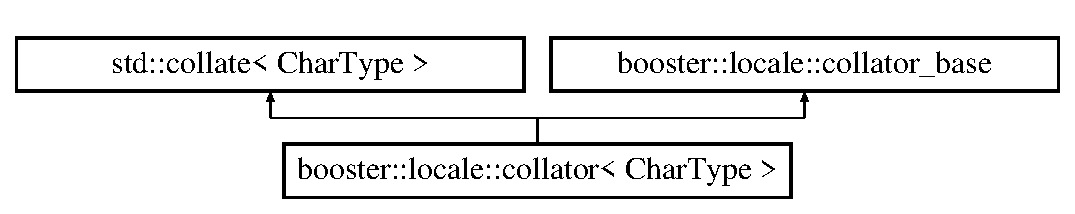
\includegraphics[height=2.000000cm]{classbooster_1_1locale_1_1collator}
\end{center}
\end{figure}
\subsection*{Public Types}
\begin{DoxyCompactItemize}
\item 
typedef Char\+Type {\bf char\+\_\+type}
\item 
typedef std\+::basic\+\_\+string$<$ Char\+Type $>$ {\bf string\+\_\+type}
\end{DoxyCompactItemize}
\subsection*{Public Member Functions}
\begin{DoxyCompactItemize}
\item 
int {\bf compare} ({\bf level\+\_\+type} level, {\bf char\+\_\+type} const $\ast$b1, {\bf char\+\_\+type} const $\ast$e1, {\bf char\+\_\+type} const $\ast$b2, {\bf char\+\_\+type} const $\ast$e2) const 
\item 
{\bf string\+\_\+type} {\bf transform} ({\bf level\+\_\+type} level, {\bf char\+\_\+type} const $\ast$b, {\bf char\+\_\+type} const $\ast$e) const 
\item 
long {\bf hash} ({\bf level\+\_\+type} level, {\bf char\+\_\+type} const $\ast$b, {\bf char\+\_\+type} const $\ast$e) const 
\item 
int {\bf compare} ({\bf level\+\_\+type} level, {\bf string\+\_\+type} const \&l, {\bf string\+\_\+type} const \&r) const 
\item 
long {\bf hash} ({\bf level\+\_\+type} level, {\bf string\+\_\+type} const \&s) const 
\item 
{\bf string\+\_\+type} {\bf transform} ({\bf level\+\_\+type} level, {\bf string\+\_\+type} const \&s) const 
\end{DoxyCompactItemize}
\subsection*{Protected Member Functions}
\begin{DoxyCompactItemize}
\item 
{\bf collator} (size\+\_\+t refs=0)
\item 
virtual int {\bf do\+\_\+compare} ({\bf char\+\_\+type} const $\ast$b1, {\bf char\+\_\+type} const $\ast$e1, {\bf char\+\_\+type} const $\ast$b2, {\bf char\+\_\+type} const $\ast$e2) const 
\item 
virtual {\bf string\+\_\+type} {\bf do\+\_\+transform} ({\bf char\+\_\+type} const $\ast$b, {\bf char\+\_\+type} const $\ast$e) const 
\item 
virtual long {\bf do\+\_\+hash} ({\bf char\+\_\+type} const $\ast$b, {\bf char\+\_\+type} const $\ast$e) const 
\item 
virtual int {\bf do\+\_\+compare} ({\bf level\+\_\+type} level, {\bf char\+\_\+type} const $\ast$b1, {\bf char\+\_\+type} const $\ast$e1, {\bf char\+\_\+type} const $\ast$b2, {\bf char\+\_\+type} const $\ast$e2) const =0
\item 
virtual {\bf string\+\_\+type} {\bf do\+\_\+transform} ({\bf level\+\_\+type} level, {\bf char\+\_\+type} const $\ast$b, {\bf char\+\_\+type} const $\ast$e) const =0
\item 
virtual long {\bf do\+\_\+hash} ({\bf level\+\_\+type} level, {\bf char\+\_\+type} const $\ast$b, {\bf char\+\_\+type} const $\ast$e) const =0
\end{DoxyCompactItemize}


\subsection{Detailed Description}
\subsubsection*{template$<$typename Char\+Type$>$\\*
class booster\+::locale\+::collator$<$ Char\+Type $>$}

Collation facet. 

It reimplements standard C++ std\+::collate, allowing usage of std\+::locale for direct string comparison 

\subsection{Member Typedef Documentation}
\index{booster\+::locale\+::collator@{booster\+::locale\+::collator}!char\+\_\+type@{char\+\_\+type}}
\index{char\+\_\+type@{char\+\_\+type}!booster\+::locale\+::collator@{booster\+::locale\+::collator}}
\subsubsection[{char\+\_\+type}]{\setlength{\rightskip}{0pt plus 5cm}template$<$typename Char\+Type $>$ typedef Char\+Type {\bf booster\+::locale\+::collator}$<$ Char\+Type $>$\+::{\bf char\+\_\+type}}\label{classbooster_1_1locale_1_1collator_ae96a8d2f1bac6295f9dbea5c5f22a009}
Type of the underlying character \index{booster\+::locale\+::collator@{booster\+::locale\+::collator}!string\+\_\+type@{string\+\_\+type}}
\index{string\+\_\+type@{string\+\_\+type}!booster\+::locale\+::collator@{booster\+::locale\+::collator}}
\subsubsection[{string\+\_\+type}]{\setlength{\rightskip}{0pt plus 5cm}template$<$typename Char\+Type $>$ typedef std\+::basic\+\_\+string$<$Char\+Type$>$ {\bf booster\+::locale\+::collator}$<$ Char\+Type $>$\+::{\bf string\+\_\+type}}\label{classbooster_1_1locale_1_1collator_a6bb8ffea195f7e4991b77eddf15e3d9f}
Type of string used with this facet 

\subsection{Constructor \& Destructor Documentation}
\index{booster\+::locale\+::collator@{booster\+::locale\+::collator}!collator@{collator}}
\index{collator@{collator}!booster\+::locale\+::collator@{booster\+::locale\+::collator}}
\subsubsection[{collator(size\+\_\+t refs=0)}]{\setlength{\rightskip}{0pt plus 5cm}template$<$typename Char\+Type $>$ {\bf booster\+::locale\+::collator}$<$ Char\+Type $>$\+::{\bf collator} (
\begin{DoxyParamCaption}
\item[{size\+\_\+t}]{refs = {\ttfamily 0}}
\end{DoxyParamCaption}
)\hspace{0.3cm}{\ttfamily [inline]}, {\ttfamily [protected]}}\label{classbooster_1_1locale_1_1collator_aa12207d0d38e355a80c2374a4a6b8595}
constructor of the collator object 

\subsection{Member Function Documentation}
\index{booster\+::locale\+::collator@{booster\+::locale\+::collator}!compare@{compare}}
\index{compare@{compare}!booster\+::locale\+::collator@{booster\+::locale\+::collator}}
\subsubsection[{compare(level\+\_\+type level, char\+\_\+type const $\ast$b1, char\+\_\+type const $\ast$e1, char\+\_\+type const $\ast$b2, char\+\_\+type const $\ast$e2) const }]{\setlength{\rightskip}{0pt plus 5cm}template$<$typename Char\+Type $>$ int {\bf booster\+::locale\+::collator}$<$ Char\+Type $>$\+::compare (
\begin{DoxyParamCaption}
\item[{{\bf level\+\_\+type}}]{level, }
\item[{{\bf char\+\_\+type} const $\ast$}]{b1, }
\item[{{\bf char\+\_\+type} const $\ast$}]{e1, }
\item[{{\bf char\+\_\+type} const $\ast$}]{b2, }
\item[{{\bf char\+\_\+type} const $\ast$}]{e2}
\end{DoxyParamCaption}
) const\hspace{0.3cm}{\ttfamily [inline]}}\label{classbooster_1_1locale_1_1collator_a7109cc3cde851e4a0f7392d7344bf97c}
Compare two strings in rage [b1,e1), [b2,e2) according using a collation level {\itshape level}. Calls do\+\_\+compare

Returns -\/1 if the first of the two strings sorts before the seconds, returns 1 if sorts after and 0 if they considered equal. \index{booster\+::locale\+::collator@{booster\+::locale\+::collator}!compare@{compare}}
\index{compare@{compare}!booster\+::locale\+::collator@{booster\+::locale\+::collator}}
\subsubsection[{compare(level\+\_\+type level, string\+\_\+type const \&l, string\+\_\+type const \&r) const }]{\setlength{\rightskip}{0pt plus 5cm}template$<$typename Char\+Type $>$ int {\bf booster\+::locale\+::collator}$<$ Char\+Type $>$\+::compare (
\begin{DoxyParamCaption}
\item[{{\bf level\+\_\+type}}]{level, }
\item[{{\bf string\+\_\+type} const \&}]{l, }
\item[{{\bf string\+\_\+type} const \&}]{r}
\end{DoxyParamCaption}
) const\hspace{0.3cm}{\ttfamily [inline]}}\label{classbooster_1_1locale_1_1collator_a2756a9012ecbf8bb026b7bf5586d564d}
Compare two strings {\itshape l} and {\itshape r} using collation level {\itshape level} 

Returns -\/1 if the first of the two strings sorts before the seconds, returns 1 if sorts after and 0 if they considered equal. \index{booster\+::locale\+::collator@{booster\+::locale\+::collator}!do\+\_\+compare@{do\+\_\+compare}}
\index{do\+\_\+compare@{do\+\_\+compare}!booster\+::locale\+::collator@{booster\+::locale\+::collator}}
\subsubsection[{do\+\_\+compare(char\+\_\+type const $\ast$b1, char\+\_\+type const $\ast$e1, char\+\_\+type const $\ast$b2, char\+\_\+type const $\ast$e2) const }]{\setlength{\rightskip}{0pt plus 5cm}template$<$typename Char\+Type $>$ virtual int {\bf booster\+::locale\+::collator}$<$ Char\+Type $>$\+::do\+\_\+compare (
\begin{DoxyParamCaption}
\item[{{\bf char\+\_\+type} const $\ast$}]{b1, }
\item[{{\bf char\+\_\+type} const $\ast$}]{e1, }
\item[{{\bf char\+\_\+type} const $\ast$}]{b2, }
\item[{{\bf char\+\_\+type} const $\ast$}]{e2}
\end{DoxyParamCaption}
) const\hspace{0.3cm}{\ttfamily [inline]}, {\ttfamily [protected]}, {\ttfamily [virtual]}}\label{classbooster_1_1locale_1_1collator_a17c522d7978bc89fd412aeb8d7809f04}
This function is used to override default collation function that does not take in account collation level. Uses primary level 

References booster\+::locale\+::collator\+\_\+base\+::identical.

\index{booster\+::locale\+::collator@{booster\+::locale\+::collator}!do\+\_\+compare@{do\+\_\+compare}}
\index{do\+\_\+compare@{do\+\_\+compare}!booster\+::locale\+::collator@{booster\+::locale\+::collator}}
\subsubsection[{do\+\_\+compare(level\+\_\+type level, char\+\_\+type const $\ast$b1, char\+\_\+type const $\ast$e1, char\+\_\+type const $\ast$b2, char\+\_\+type const $\ast$e2) const =0}]{\setlength{\rightskip}{0pt plus 5cm}template$<$typename Char\+Type $>$ virtual int {\bf booster\+::locale\+::collator}$<$ Char\+Type $>$\+::do\+\_\+compare (
\begin{DoxyParamCaption}
\item[{{\bf level\+\_\+type}}]{level, }
\item[{{\bf char\+\_\+type} const $\ast$}]{b1, }
\item[{{\bf char\+\_\+type} const $\ast$}]{e1, }
\item[{{\bf char\+\_\+type} const $\ast$}]{b2, }
\item[{{\bf char\+\_\+type} const $\ast$}]{e2}
\end{DoxyParamCaption}
) const\hspace{0.3cm}{\ttfamily [protected]}, {\ttfamily [pure virtual]}}\label{classbooster_1_1locale_1_1collator_ad8e79f03cdc362a9195eb81a15f626bd}
Actual function that performs comparison between the strings. For details see compare member function. Can be overridden. \index{booster\+::locale\+::collator@{booster\+::locale\+::collator}!do\+\_\+hash@{do\+\_\+hash}}
\index{do\+\_\+hash@{do\+\_\+hash}!booster\+::locale\+::collator@{booster\+::locale\+::collator}}
\subsubsection[{do\+\_\+hash(char\+\_\+type const $\ast$b, char\+\_\+type const $\ast$e) const }]{\setlength{\rightskip}{0pt plus 5cm}template$<$typename Char\+Type $>$ virtual long {\bf booster\+::locale\+::collator}$<$ Char\+Type $>$\+::do\+\_\+hash (
\begin{DoxyParamCaption}
\item[{{\bf char\+\_\+type} const $\ast$}]{b, }
\item[{{\bf char\+\_\+type} const $\ast$}]{e}
\end{DoxyParamCaption}
) const\hspace{0.3cm}{\ttfamily [inline]}, {\ttfamily [protected]}, {\ttfamily [virtual]}}\label{classbooster_1_1locale_1_1collator_ab69f3a6a0e13ae1c1d589e6b5b8f7c6e}
This function is used to override default collation function that does not take in account collation level. Uses primary level 

References booster\+::locale\+::collator\+\_\+base\+::identical.

\index{booster\+::locale\+::collator@{booster\+::locale\+::collator}!do\+\_\+hash@{do\+\_\+hash}}
\index{do\+\_\+hash@{do\+\_\+hash}!booster\+::locale\+::collator@{booster\+::locale\+::collator}}
\subsubsection[{do\+\_\+hash(level\+\_\+type level, char\+\_\+type const $\ast$b, char\+\_\+type const $\ast$e) const =0}]{\setlength{\rightskip}{0pt plus 5cm}template$<$typename Char\+Type $>$ virtual long {\bf booster\+::locale\+::collator}$<$ Char\+Type $>$\+::do\+\_\+hash (
\begin{DoxyParamCaption}
\item[{{\bf level\+\_\+type}}]{level, }
\item[{{\bf char\+\_\+type} const $\ast$}]{b, }
\item[{{\bf char\+\_\+type} const $\ast$}]{e}
\end{DoxyParamCaption}
) const\hspace{0.3cm}{\ttfamily [protected]}, {\ttfamily [pure virtual]}}\label{classbooster_1_1locale_1_1collator_ae412e2daa978d73472945ef6e9a4f9f4}
Actual function that calculates hash. For details see hash member function. Can be overridden. \index{booster\+::locale\+::collator@{booster\+::locale\+::collator}!do\+\_\+transform@{do\+\_\+transform}}
\index{do\+\_\+transform@{do\+\_\+transform}!booster\+::locale\+::collator@{booster\+::locale\+::collator}}
\subsubsection[{do\+\_\+transform(char\+\_\+type const $\ast$b, char\+\_\+type const $\ast$e) const }]{\setlength{\rightskip}{0pt plus 5cm}template$<$typename Char\+Type $>$ virtual {\bf string\+\_\+type} {\bf booster\+::locale\+::collator}$<$ Char\+Type $>$\+::do\+\_\+transform (
\begin{DoxyParamCaption}
\item[{{\bf char\+\_\+type} const $\ast$}]{b, }
\item[{{\bf char\+\_\+type} const $\ast$}]{e}
\end{DoxyParamCaption}
) const\hspace{0.3cm}{\ttfamily [inline]}, {\ttfamily [protected]}, {\ttfamily [virtual]}}\label{classbooster_1_1locale_1_1collator_ab03d39b5d1948c53ae755bbc1c6f8908}
This function is used to override default collation function that does not take in account collation level. Uses primary level 

References booster\+::locale\+::collator\+\_\+base\+::identical.

\index{booster\+::locale\+::collator@{booster\+::locale\+::collator}!do\+\_\+transform@{do\+\_\+transform}}
\index{do\+\_\+transform@{do\+\_\+transform}!booster\+::locale\+::collator@{booster\+::locale\+::collator}}
\subsubsection[{do\+\_\+transform(level\+\_\+type level, char\+\_\+type const $\ast$b, char\+\_\+type const $\ast$e) const =0}]{\setlength{\rightskip}{0pt plus 5cm}template$<$typename Char\+Type $>$ virtual {\bf string\+\_\+type} {\bf booster\+::locale\+::collator}$<$ Char\+Type $>$\+::do\+\_\+transform (
\begin{DoxyParamCaption}
\item[{{\bf level\+\_\+type}}]{level, }
\item[{{\bf char\+\_\+type} const $\ast$}]{b, }
\item[{{\bf char\+\_\+type} const $\ast$}]{e}
\end{DoxyParamCaption}
) const\hspace{0.3cm}{\ttfamily [protected]}, {\ttfamily [pure virtual]}}\label{classbooster_1_1locale_1_1collator_a6ff91d0873d513db245f6f44f66b6170}
Actual function that performs transformation. For details see transform member function. Can be overridden. \index{booster\+::locale\+::collator@{booster\+::locale\+::collator}!hash@{hash}}
\index{hash@{hash}!booster\+::locale\+::collator@{booster\+::locale\+::collator}}
\subsubsection[{hash(level\+\_\+type level, char\+\_\+type const $\ast$b, char\+\_\+type const $\ast$e) const }]{\setlength{\rightskip}{0pt plus 5cm}template$<$typename Char\+Type $>$ long {\bf booster\+::locale\+::collator}$<$ Char\+Type $>$\+::hash (
\begin{DoxyParamCaption}
\item[{{\bf level\+\_\+type}}]{level, }
\item[{{\bf char\+\_\+type} const $\ast$}]{b, }
\item[{{\bf char\+\_\+type} const $\ast$}]{e}
\end{DoxyParamCaption}
) const\hspace{0.3cm}{\ttfamily [inline]}}\label{classbooster_1_1locale_1_1collator_a641910a6170fdcbea24ab8061657397a}
Calculate a hash of a text in range [b,e). The value can be used for collation sensitive string comparison.

If compare(level,b1,e1,b2,e2) == 0 then hash(level,b1,e1) == hash(level,b2,e2)

Calls do\+\_\+hash \index{booster\+::locale\+::collator@{booster\+::locale\+::collator}!hash@{hash}}
\index{hash@{hash}!booster\+::locale\+::collator@{booster\+::locale\+::collator}}
\subsubsection[{hash(level\+\_\+type level, string\+\_\+type const \&s) const }]{\setlength{\rightskip}{0pt plus 5cm}template$<$typename Char\+Type $>$ long {\bf booster\+::locale\+::collator}$<$ Char\+Type $>$\+::hash (
\begin{DoxyParamCaption}
\item[{{\bf level\+\_\+type}}]{level, }
\item[{{\bf string\+\_\+type} const \&}]{s}
\end{DoxyParamCaption}
) const\hspace{0.3cm}{\ttfamily [inline]}}\label{classbooster_1_1locale_1_1collator_a8c6ae3d41166e2e43d15e97efe1ffa5e}
Calculate a hash that can be used for collation sensitive string comparison of a string {\itshape s} 

If compare(level,s1,s2) == 0 then hash(level,s1) == hash(level,s2) \index{booster\+::locale\+::collator@{booster\+::locale\+::collator}!transform@{transform}}
\index{transform@{transform}!booster\+::locale\+::collator@{booster\+::locale\+::collator}}
\subsubsection[{transform(level\+\_\+type level, char\+\_\+type const $\ast$b, char\+\_\+type const $\ast$e) const }]{\setlength{\rightskip}{0pt plus 5cm}template$<$typename Char\+Type $>$ {\bf string\+\_\+type} {\bf booster\+::locale\+::collator}$<$ Char\+Type $>$\+::transform (
\begin{DoxyParamCaption}
\item[{{\bf level\+\_\+type}}]{level, }
\item[{{\bf char\+\_\+type} const $\ast$}]{b, }
\item[{{\bf char\+\_\+type} const $\ast$}]{e}
\end{DoxyParamCaption}
) const\hspace{0.3cm}{\ttfamily [inline]}}\label{classbooster_1_1locale_1_1collator_a475ed44666b45e8ef0570e0ec8f45762}
Create a binary string that can be compared to other in order to get collation order. The string is created for text in range [b,e). It is useful for collation of multiple strings for text.

The transformation follows these rules\+: 
\begin{DoxyCode}
compare(level,b1,e1,b2,e2) == sign( transform(level,b1,e1).compare(transform(level,b2,e2)) );
\end{DoxyCode}


Calls do\+\_\+transform \index{booster\+::locale\+::collator@{booster\+::locale\+::collator}!transform@{transform}}
\index{transform@{transform}!booster\+::locale\+::collator@{booster\+::locale\+::collator}}
\subsubsection[{transform(level\+\_\+type level, string\+\_\+type const \&s) const }]{\setlength{\rightskip}{0pt plus 5cm}template$<$typename Char\+Type $>$ {\bf string\+\_\+type} {\bf booster\+::locale\+::collator}$<$ Char\+Type $>$\+::transform (
\begin{DoxyParamCaption}
\item[{{\bf level\+\_\+type}}]{level, }
\item[{{\bf string\+\_\+type} const \&}]{s}
\end{DoxyParamCaption}
) const\hspace{0.3cm}{\ttfamily [inline]}}\label{classbooster_1_1locale_1_1collator_abc3529e97d5793124bb7a7809217f87f}
Create a binary string from string {\itshape s}, that can be compared to other, useful for collation of multiple strings.

The transformation follows these rules\+: 
\begin{DoxyCode}
compare(level,s1,s2) == sign( transform(level,s1).compare(transform(level,s2)) );
\end{DoxyCode}
 

The documentation for this class was generated from the following file\+:\begin{DoxyCompactItemize}
\item 
booster/locale/collator.\+h\end{DoxyCompactItemize}

\section{booster\+:\+:locale\+:\+:collator\+\_\+base Class Reference}
\label{classbooster_1_1locale_1_1collator__base}\index{booster\+::locale\+::collator\+\_\+base@{booster\+::locale\+::collator\+\_\+base}}


a base class that includes collation level flags  




{\ttfamily \#include $<$booster/booster/locale/collator.\+h$>$}

Inheritance diagram for booster\+:\+:locale\+:\+:collator\+\_\+base\+:\begin{figure}[H]
\begin{center}
\leavevmode
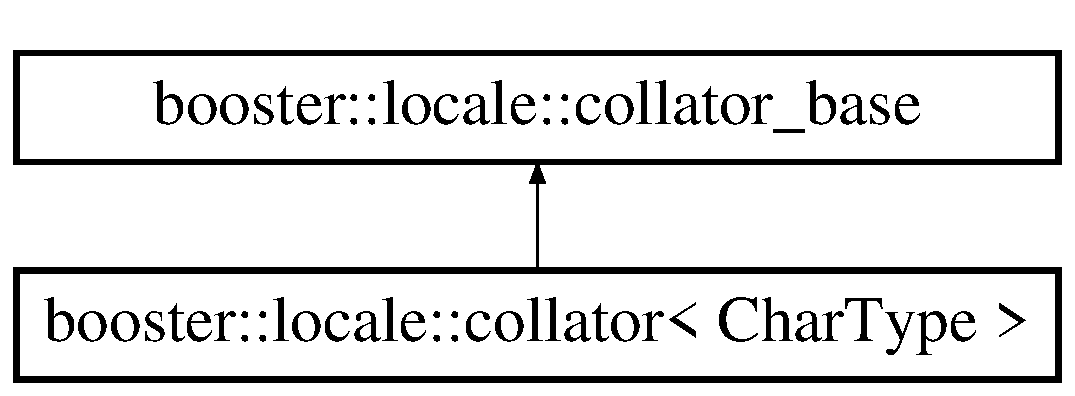
\includegraphics[height=2.000000cm]{classbooster_1_1locale_1_1collator__base}
\end{center}
\end{figure}
\subsection*{Public Types}
\begin{DoxyCompactItemize}
\item 
enum {\bf level\+\_\+type} \{ \\*
{\bf primary} = 0, 
{\bf secondary} = 1, 
{\bf tertiary} = 2, 
{\bf quaternary} = 3, 
\\*
{\bf identical} = 4
 \}
\end{DoxyCompactItemize}


\subsection{Detailed Description}
a base class that includes collation level flags 

\subsection{Member Enumeration Documentation}
\index{booster\+::locale\+::collator\+\_\+base@{booster\+::locale\+::collator\+\_\+base}!level\+\_\+type@{level\+\_\+type}}
\index{level\+\_\+type@{level\+\_\+type}!booster\+::locale\+::collator\+\_\+base@{booster\+::locale\+::collator\+\_\+base}}
\subsubsection[{level\+\_\+type}]{\setlength{\rightskip}{0pt plus 5cm}enum {\bf booster\+::locale\+::collator\+\_\+base\+::level\+\_\+type}}\label{classbooster_1_1locale_1_1collator__base_aa97842d22c5b274d85c9f6028424ca72}
Unicode collation level types \begin{Desc}
\item[Enumerator]\par
\begin{description}
\index{primary@{primary}!booster\+::locale\+::collator\+\_\+base@{booster\+::locale\+::collator\+\_\+base}}\index{booster\+::locale\+::collator\+\_\+base@{booster\+::locale\+::collator\+\_\+base}!primary@{primary}}\item[{\em 
primary\label{classbooster_1_1locale_1_1collator__base_aa97842d22c5b274d85c9f6028424ca72a98fba217ca6b058fdcb9535052854c94}
}]1st collation level\+: base letters \index{secondary@{secondary}!booster\+::locale\+::collator\+\_\+base@{booster\+::locale\+::collator\+\_\+base}}\index{booster\+::locale\+::collator\+\_\+base@{booster\+::locale\+::collator\+\_\+base}!secondary@{secondary}}\item[{\em 
secondary\label{classbooster_1_1locale_1_1collator__base_aa97842d22c5b274d85c9f6028424ca72ad5f5fb07eda062123c7e11323db12b72}
}]2nd collation level\+: letters and accents \index{tertiary@{tertiary}!booster\+::locale\+::collator\+\_\+base@{booster\+::locale\+::collator\+\_\+base}}\index{booster\+::locale\+::collator\+\_\+base@{booster\+::locale\+::collator\+\_\+base}!tertiary@{tertiary}}\item[{\em 
tertiary\label{classbooster_1_1locale_1_1collator__base_aa97842d22c5b274d85c9f6028424ca72a8f84ab2f5d92e21b265f687ebc061702}
}]3rd collation level\+: letters, accents and case \index{quaternary@{quaternary}!booster\+::locale\+::collator\+\_\+base@{booster\+::locale\+::collator\+\_\+base}}\index{booster\+::locale\+::collator\+\_\+base@{booster\+::locale\+::collator\+\_\+base}!quaternary@{quaternary}}\item[{\em 
quaternary\label{classbooster_1_1locale_1_1collator__base_aa97842d22c5b274d85c9f6028424ca72a614e0d98df0df4b2524ee8a9ca6f8f68}
}]4th collation level\+: letters, accents, case and punctuation \index{identical@{identical}!booster\+::locale\+::collator\+\_\+base@{booster\+::locale\+::collator\+\_\+base}}\index{booster\+::locale\+::collator\+\_\+base@{booster\+::locale\+::collator\+\_\+base}!identical@{identical}}\item[{\em 
identical\label{classbooster_1_1locale_1_1collator__base_aa97842d22c5b274d85c9f6028424ca72ada307519aa53e82b463654668a6541e2}
}]identical collation level\+: include code-\/point comparison \end{description}
\end{Desc}


The documentation for this class was generated from the following file\+:\begin{DoxyCompactItemize}
\item 
booster/locale/collator.\+h\end{DoxyCompactItemize}

\section{booster\+:\+:locale\+:\+:comparator$<$ Char\+Type, default\+\_\+level $>$ Struct Template Reference}
\label{structbooster_1_1locale_1_1comparator}\index{booster\+::locale\+::comparator$<$ Char\+Type, default\+\_\+level $>$@{booster\+::locale\+::comparator$<$ Char\+Type, default\+\_\+level $>$}}


This class can be used in S\+TL algorithms and containers for comparison of strings with a level other than primary.  




{\ttfamily \#include $<$booster/booster/locale/collator.\+h$>$}

\subsection*{Public Member Functions}
\begin{DoxyCompactItemize}
\item 
{\bf comparator} (std\+::locale const \&l=std\+::locale(), {\bf collator\+\_\+base\+::level\+\_\+type} level=default\+\_\+level)
\item 
bool {\bf operator()} (std\+::basic\+\_\+string$<$ Char\+Type $>$ const \&left, std\+::basic\+\_\+string$<$ Char\+Type $>$ const \&right) const 
\end{DoxyCompactItemize}


\subsection{Detailed Description}
\subsubsection*{template$<$typename Char\+Type, collator\+\_\+base\+::level\+\_\+type default\+\_\+level = collator\+\_\+base\+::identical$>$\\*
struct booster\+::locale\+::comparator$<$ Char\+Type, default\+\_\+level $>$}

This class can be used in S\+TL algorithms and containers for comparison of strings with a level other than primary. 

For example\+:


\begin{DoxyCode}
std::map<std::string,std::string,comparator<char,collator\_base::secondary> > data;
\end{DoxyCode}


Would create a map the keys of which are sorted using secondary collation level 

\subsection{Constructor \& Destructor Documentation}
\index{booster\+::locale\+::comparator@{booster\+::locale\+::comparator}!comparator@{comparator}}
\index{comparator@{comparator}!booster\+::locale\+::comparator@{booster\+::locale\+::comparator}}
\subsubsection[{comparator(std\+::locale const \&l=std\+::locale(), collator\+\_\+base\+::level\+\_\+type level=default\+\_\+level)}]{\setlength{\rightskip}{0pt plus 5cm}template$<$typename Char\+Type , collator\+\_\+base\+::level\+\_\+type default\+\_\+level = collator\+\_\+base\+::identical$>$ {\bf booster\+::locale\+::comparator}$<$ Char\+Type, default\+\_\+level $>$\+::{\bf comparator} (
\begin{DoxyParamCaption}
\item[{std\+::locale const \&}]{l = {\ttfamily std\+:\+:locale()}, }
\item[{{\bf collator\+\_\+base\+::level\+\_\+type}}]{level = {\ttfamily default\+\_\+level}}
\end{DoxyParamCaption}
)\hspace{0.3cm}{\ttfamily [inline]}}\label{structbooster_1_1locale_1_1comparator_a91b9aefe26b288fdf17890a3b1d61597}
Create a comparator class for locale {\itshape l} and with collation leval {\itshape level} 

\begin{DoxyNote}{Note}
throws std\+::bad\+\_\+cast if l does not have \doxyref{collator}{p.}{classbooster_1_1locale_1_1collator} facet installed 
\end{DoxyNote}


\subsection{Member Function Documentation}
\index{booster\+::locale\+::comparator@{booster\+::locale\+::comparator}!operator()@{operator()}}
\index{operator()@{operator()}!booster\+::locale\+::comparator@{booster\+::locale\+::comparator}}
\subsubsection[{operator()(std\+::basic\+\_\+string$<$ Char\+Type $>$ const \&left, std\+::basic\+\_\+string$<$ Char\+Type $>$ const \&right) const }]{\setlength{\rightskip}{0pt plus 5cm}template$<$typename Char\+Type , collator\+\_\+base\+::level\+\_\+type default\+\_\+level = collator\+\_\+base\+::identical$>$ bool {\bf booster\+::locale\+::comparator}$<$ Char\+Type, default\+\_\+level $>$\+::operator() (
\begin{DoxyParamCaption}
\item[{std\+::basic\+\_\+string$<$ Char\+Type $>$ const \&}]{left, }
\item[{std\+::basic\+\_\+string$<$ Char\+Type $>$ const \&}]{right}
\end{DoxyParamCaption}
) const\hspace{0.3cm}{\ttfamily [inline]}}\label{structbooster_1_1locale_1_1comparator_a9f4726246672b08cd9a30d7431f6945d}
Compare two strings -- equivalent to return left $<$ right according to collation rules 

The documentation for this struct was generated from the following file\+:\begin{DoxyCompactItemize}
\item 
booster/locale/collator.\+h\end{DoxyCompactItemize}

\section{booster\+:\+:aio\+:\+:const\+\_\+buffer Class Reference}
\label{classbooster_1_1aio_1_1const__buffer}\index{booster\+::aio\+::const\+\_\+buffer@{booster\+::aio\+::const\+\_\+buffer}}


An immutable buffer -\/ buffer for write operations.  




{\ttfamily \#include $<$booster/booster/aio/buffer.\+h$>$}

Inheritance diagram for booster\+:\+:aio\+:\+:const\+\_\+buffer\+:\begin{figure}[H]
\begin{center}
\leavevmode
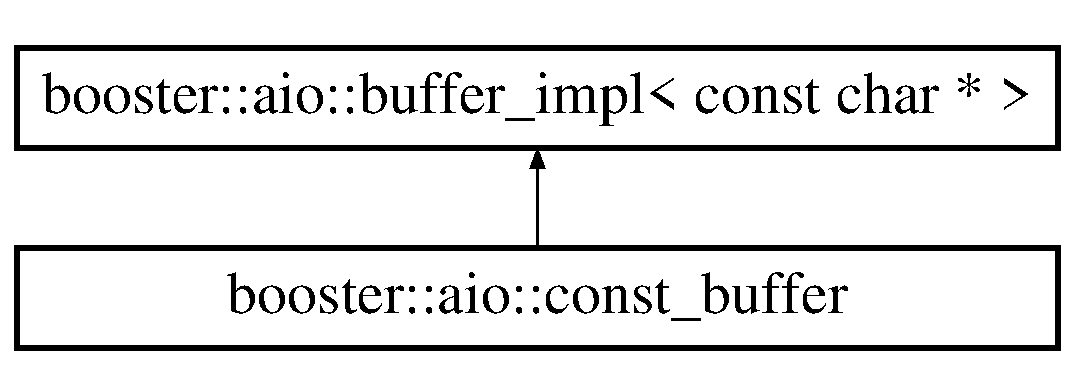
\includegraphics[height=2.000000cm]{classbooster_1_1aio_1_1const__buffer}
\end{center}
\end{figure}
\subsection*{Public Member Functions}
\begin{DoxyCompactItemize}
\item 
{\bf const\+\_\+buffer} ({\bf mutable\+\_\+buffer} const \&other)
\end{DoxyCompactItemize}
\subsection*{Additional Inherited Members}


\subsection{Detailed Description}
An immutable buffer -\/ buffer for write operations. 

\subsection{Constructor \& Destructor Documentation}
\index{booster\+::aio\+::const\+\_\+buffer@{booster\+::aio\+::const\+\_\+buffer}!const\+\_\+buffer@{const\+\_\+buffer}}
\index{const\+\_\+buffer@{const\+\_\+buffer}!booster\+::aio\+::const\+\_\+buffer@{booster\+::aio\+::const\+\_\+buffer}}
\subsubsection[{const\+\_\+buffer(mutable\+\_\+buffer const \&other)}]{\setlength{\rightskip}{0pt plus 5cm}booster\+::aio\+::const\+\_\+buffer\+::const\+\_\+buffer (
\begin{DoxyParamCaption}
\item[{{\bf mutable\+\_\+buffer} const \&}]{other}
\end{DoxyParamCaption}
)\hspace{0.3cm}{\ttfamily [inline]}}\label{classbooster_1_1aio_1_1const__buffer_a5b0f4961bac497135a6a0f517a56e354}
Create a const buffer from mutable buffer 

References booster\+::aio\+::buffer\+\_\+impl$<$ Pointer $>$\+::add(), and booster\+::aio\+::buffer\+\_\+impl$<$ Pointer $>$\+::get().



The documentation for this class was generated from the following file\+:\begin{DoxyCompactItemize}
\item 
booster/aio/buffer.\+h\end{DoxyCompactItemize}

\section{cppcms\+:\+:util\+:\+:const\+\_\+char\+\_\+buf Class Reference}
\label{classcppcms_1_1util_1_1const__char__buf}\index{cppcms\+::util\+::const\+\_\+char\+\_\+buf@{cppcms\+::util\+::const\+\_\+char\+\_\+buf}}


{\ttfamily \#include $<$cppcms/steal\+\_\+buf.\+h$>$}

Inheritance diagram for cppcms\+:\+:util\+:\+:const\+\_\+char\+\_\+buf\+:\begin{figure}[H]
\begin{center}
\leavevmode
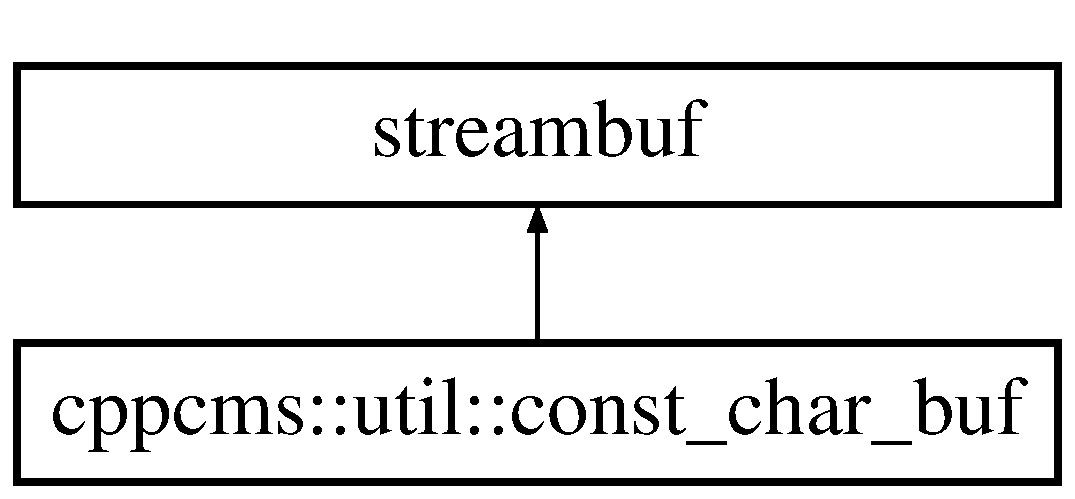
\includegraphics[height=2.000000cm]{classcppcms_1_1util_1_1const__char__buf}
\end{center}
\end{figure}
\subsection*{Public Member Functions}
\begin{DoxyCompactItemize}
\item 
{\bf const\+\_\+char\+\_\+buf} ()
\item 
{\bf const\+\_\+char\+\_\+buf} (char const $\ast${\bf begin}, char const $\ast${\bf end})
\item 
void {\bf range} (char const $\ast$cbegin, char const $\ast$cend)
\item 
char const $\ast$ {\bf begin} () const 
\item 
char const $\ast$ {\bf end} () const 
\end{DoxyCompactItemize}


\subsection{Detailed Description}
Simple std\+::streambuf to create input from [char const $\ast$,char const $\ast$) range

\doxyref{New in Cpp\+C\+MS 1.\+2}{p.}{v1_2} 

\subsection{Constructor \& Destructor Documentation}
\index{cppcms\+::util\+::const\+\_\+char\+\_\+buf@{cppcms\+::util\+::const\+\_\+char\+\_\+buf}!const\+\_\+char\+\_\+buf@{const\+\_\+char\+\_\+buf}}
\index{const\+\_\+char\+\_\+buf@{const\+\_\+char\+\_\+buf}!cppcms\+::util\+::const\+\_\+char\+\_\+buf@{cppcms\+::util\+::const\+\_\+char\+\_\+buf}}
\subsubsection[{const\+\_\+char\+\_\+buf()}]{\setlength{\rightskip}{0pt plus 5cm}cppcms\+::util\+::const\+\_\+char\+\_\+buf\+::const\+\_\+char\+\_\+buf (
\begin{DoxyParamCaption}
{}
\end{DoxyParamCaption}
)\hspace{0.3cm}{\ttfamily [inline]}}\label{classcppcms_1_1util_1_1const__char__buf_aa9ffb8af281415989591937c147798c8}
Create Empty buffer 

References range().

\index{cppcms\+::util\+::const\+\_\+char\+\_\+buf@{cppcms\+::util\+::const\+\_\+char\+\_\+buf}!const\+\_\+char\+\_\+buf@{const\+\_\+char\+\_\+buf}}
\index{const\+\_\+char\+\_\+buf@{const\+\_\+char\+\_\+buf}!cppcms\+::util\+::const\+\_\+char\+\_\+buf@{cppcms\+::util\+::const\+\_\+char\+\_\+buf}}
\subsubsection[{const\+\_\+char\+\_\+buf(char const $\ast$begin, char const $\ast$end)}]{\setlength{\rightskip}{0pt plus 5cm}cppcms\+::util\+::const\+\_\+char\+\_\+buf\+::const\+\_\+char\+\_\+buf (
\begin{DoxyParamCaption}
\item[{char const $\ast$}]{begin, }
\item[{char const $\ast$}]{end}
\end{DoxyParamCaption}
)\hspace{0.3cm}{\ttfamily [inline]}}\label{classcppcms_1_1util_1_1const__char__buf_accdec5e05e4611fe5d2536376dc3ae9b}
Create a buffer from a range 

References range().



\subsection{Member Function Documentation}
\index{cppcms\+::util\+::const\+\_\+char\+\_\+buf@{cppcms\+::util\+::const\+\_\+char\+\_\+buf}!begin@{begin}}
\index{begin@{begin}!cppcms\+::util\+::const\+\_\+char\+\_\+buf@{cppcms\+::util\+::const\+\_\+char\+\_\+buf}}
\subsubsection[{begin() const }]{\setlength{\rightskip}{0pt plus 5cm}char const$\ast$ cppcms\+::util\+::const\+\_\+char\+\_\+buf\+::begin (
\begin{DoxyParamCaption}
{}
\end{DoxyParamCaption}
) const\hspace{0.3cm}{\ttfamily [inline]}}\label{classcppcms_1_1util_1_1const__char__buf_a73fe3026fedd9050ab3bb07464916e7d}
Begin of range 

Referenced by cppcms\+::util\+::stackbuf$<$ Size $>$\+::c\+\_\+str(), range(), and cppcms\+::util\+::stackbuf$<$ Size $>$\+::str().

\index{cppcms\+::util\+::const\+\_\+char\+\_\+buf@{cppcms\+::util\+::const\+\_\+char\+\_\+buf}!end@{end}}
\index{end@{end}!cppcms\+::util\+::const\+\_\+char\+\_\+buf@{cppcms\+::util\+::const\+\_\+char\+\_\+buf}}
\subsubsection[{end() const }]{\setlength{\rightskip}{0pt plus 5cm}char const$\ast$ cppcms\+::util\+::const\+\_\+char\+\_\+buf\+::end (
\begin{DoxyParamCaption}
{}
\end{DoxyParamCaption}
) const\hspace{0.3cm}{\ttfamily [inline]}}\label{classcppcms_1_1util_1_1const__char__buf_add3d2312a19c78cc39b76aeca06ed045}
End of range 

Referenced by range(), and cppcms\+::util\+::stackbuf$<$ Size $>$\+::str().

\index{cppcms\+::util\+::const\+\_\+char\+\_\+buf@{cppcms\+::util\+::const\+\_\+char\+\_\+buf}!range@{range}}
\index{range@{range}!cppcms\+::util\+::const\+\_\+char\+\_\+buf@{cppcms\+::util\+::const\+\_\+char\+\_\+buf}}
\subsubsection[{range(char const $\ast$cbegin, char const $\ast$cend)}]{\setlength{\rightskip}{0pt plus 5cm}void cppcms\+::util\+::const\+\_\+char\+\_\+buf\+::range (
\begin{DoxyParamCaption}
\item[{char const $\ast$}]{cbegin, }
\item[{char const $\ast$}]{cend}
\end{DoxyParamCaption}
)\hspace{0.3cm}{\ttfamily [inline]}}\label{classcppcms_1_1util_1_1const__char__buf_ac96417b8d51a9b24b4d315cb75edd687}
Define the range for existing buffer, pointer is reset to begin 

References begin(), and end().



Referenced by const\+\_\+char\+\_\+buf().



The documentation for this class was generated from the following file\+:\begin{DoxyCompactItemize}
\item 
cppcms/steal\+\_\+buf.\+h\end{DoxyCompactItemize}

\section{cppcms\+:\+:util\+:\+:const\+\_\+char\+\_\+istream Class Reference}
\label{classcppcms_1_1util_1_1const__char__istream}\index{cppcms\+::util\+::const\+\_\+char\+\_\+istream@{cppcms\+::util\+::const\+\_\+char\+\_\+istream}}


{\ttfamily \#include $<$cppcms/steal\+\_\+buf.\+h$>$}

Inheritance diagram for cppcms\+:\+:util\+:\+:const\+\_\+char\+\_\+istream\+:\begin{figure}[H]
\begin{center}
\leavevmode
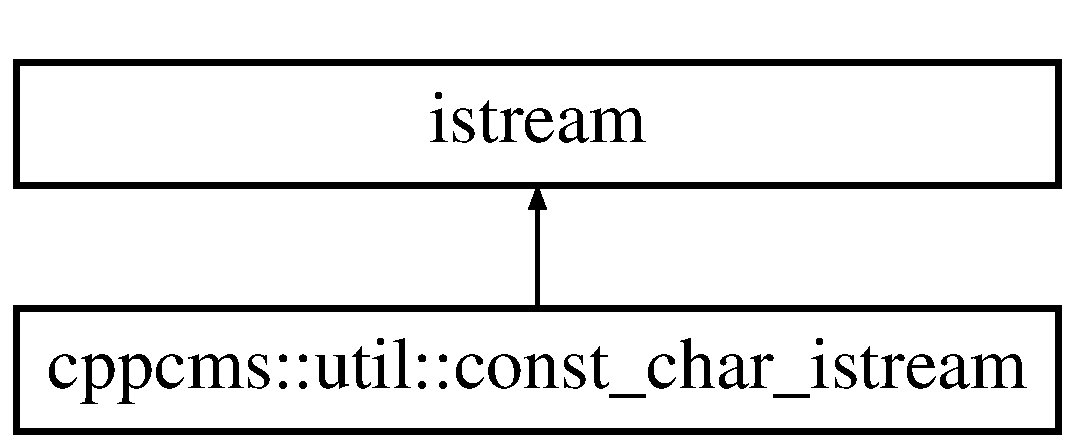
\includegraphics[height=2.000000cm]{classcppcms_1_1util_1_1const__char__istream}
\end{center}
\end{figure}
\subsection*{Public Member Functions}
\begin{DoxyCompactItemize}
\item 
{\bf const\+\_\+char\+\_\+istream} ()
\item 
{\bf const\+\_\+char\+\_\+istream} (char const $\ast${\bf begin}, char const $\ast${\bf end})
\item 
char const $\ast$ {\bf begin} () const 
\item 
char const $\ast$ {\bf end} () const 
\item 
void {\bf range} (char const $\ast${\bf begin}, char const $\ast${\bf end})
\end{DoxyCompactItemize}


\subsection{Detailed Description}
Simple std\+::istream implementation for range of [char const $\ast$,char const $\ast$)

\doxyref{New in Cpp\+C\+MS 1.\+2}{p.}{v1_2} 

\subsection{Constructor \& Destructor Documentation}
\index{cppcms\+::util\+::const\+\_\+char\+\_\+istream@{cppcms\+::util\+::const\+\_\+char\+\_\+istream}!const\+\_\+char\+\_\+istream@{const\+\_\+char\+\_\+istream}}
\index{const\+\_\+char\+\_\+istream@{const\+\_\+char\+\_\+istream}!cppcms\+::util\+::const\+\_\+char\+\_\+istream@{cppcms\+::util\+::const\+\_\+char\+\_\+istream}}
\subsubsection[{const\+\_\+char\+\_\+istream()}]{\setlength{\rightskip}{0pt plus 5cm}cppcms\+::util\+::const\+\_\+char\+\_\+istream\+::const\+\_\+char\+\_\+istream (
\begin{DoxyParamCaption}
{}
\end{DoxyParamCaption}
)\hspace{0.3cm}{\ttfamily [inline]}}\label{classcppcms_1_1util_1_1const__char__istream_aeada5cc12dfcffdc473f91c041897a38}
Create new empty stream \index{cppcms\+::util\+::const\+\_\+char\+\_\+istream@{cppcms\+::util\+::const\+\_\+char\+\_\+istream}!const\+\_\+char\+\_\+istream@{const\+\_\+char\+\_\+istream}}
\index{const\+\_\+char\+\_\+istream@{const\+\_\+char\+\_\+istream}!cppcms\+::util\+::const\+\_\+char\+\_\+istream@{cppcms\+::util\+::const\+\_\+char\+\_\+istream}}
\subsubsection[{const\+\_\+char\+\_\+istream(char const $\ast$begin, char const $\ast$end)}]{\setlength{\rightskip}{0pt plus 5cm}cppcms\+::util\+::const\+\_\+char\+\_\+istream\+::const\+\_\+char\+\_\+istream (
\begin{DoxyParamCaption}
\item[{char const $\ast$}]{begin, }
\item[{char const $\ast$}]{end}
\end{DoxyParamCaption}
)\hspace{0.3cm}{\ttfamily [inline]}}\label{classcppcms_1_1util_1_1const__char__istream_ad0a96b95b64803c83e32e1947d78db43}
Create stream initialized with range [begin,end) 

\subsection{Member Function Documentation}
\index{cppcms\+::util\+::const\+\_\+char\+\_\+istream@{cppcms\+::util\+::const\+\_\+char\+\_\+istream}!begin@{begin}}
\index{begin@{begin}!cppcms\+::util\+::const\+\_\+char\+\_\+istream@{cppcms\+::util\+::const\+\_\+char\+\_\+istream}}
\subsubsection[{begin() const }]{\setlength{\rightskip}{0pt plus 5cm}char const$\ast$ cppcms\+::util\+::const\+\_\+char\+\_\+istream\+::begin (
\begin{DoxyParamCaption}
{}
\end{DoxyParamCaption}
) const\hspace{0.3cm}{\ttfamily [inline]}}\label{classcppcms_1_1util_1_1const__char__istream_a4dc84c42e58a9456a43e3d596f54b3ba}
Get begin of the range 

Referenced by cppcms\+::parse\+\_\+url\+\_\+parameter().

\index{cppcms\+::util\+::const\+\_\+char\+\_\+istream@{cppcms\+::util\+::const\+\_\+char\+\_\+istream}!end@{end}}
\index{end@{end}!cppcms\+::util\+::const\+\_\+char\+\_\+istream@{cppcms\+::util\+::const\+\_\+char\+\_\+istream}}
\subsubsection[{end() const }]{\setlength{\rightskip}{0pt plus 5cm}char const$\ast$ cppcms\+::util\+::const\+\_\+char\+\_\+istream\+::end (
\begin{DoxyParamCaption}
{}
\end{DoxyParamCaption}
) const\hspace{0.3cm}{\ttfamily [inline]}}\label{classcppcms_1_1util_1_1const__char__istream_a9e46a22615654c1f7c13852586eb7fc8}
Get end of the range 

Referenced by cppcms\+::parse\+\_\+url\+\_\+parameter().

\index{cppcms\+::util\+::const\+\_\+char\+\_\+istream@{cppcms\+::util\+::const\+\_\+char\+\_\+istream}!range@{range}}
\index{range@{range}!cppcms\+::util\+::const\+\_\+char\+\_\+istream@{cppcms\+::util\+::const\+\_\+char\+\_\+istream}}
\subsubsection[{range(char const $\ast$begin, char const $\ast$end)}]{\setlength{\rightskip}{0pt plus 5cm}void cppcms\+::util\+::const\+\_\+char\+\_\+istream\+::range (
\begin{DoxyParamCaption}
\item[{char const $\ast$}]{begin, }
\item[{char const $\ast$}]{end}
\end{DoxyParamCaption}
)\hspace{0.3cm}{\ttfamily [inline]}}\label{classcppcms_1_1util_1_1const__char__istream_af64c02593812e450e3795e7ab8e7fdac}
Set range, resets pointer to start and clears flags 

Referenced by cppcms\+::url\+\_\+dispatcher\+::assign().



The documentation for this class was generated from the following file\+:\begin{DoxyCompactItemize}
\item 
cppcms/steal\+\_\+buf.\+h\end{DoxyCompactItemize}

\section{cppcms\+:\+:http\+:\+:content\+\_\+limits Class Reference}
\label{classcppcms_1_1http_1_1content__limits}\index{cppcms\+::http\+::content\+\_\+limits@{cppcms\+::http\+::content\+\_\+limits}}


{\ttfamily \#include $<$cppcms/http\+\_\+content\+\_\+filter.\+h$>$}

Inheritance diagram for cppcms\+:\+:http\+:\+:content\+\_\+limits\+:\begin{figure}[H]
\begin{center}
\leavevmode
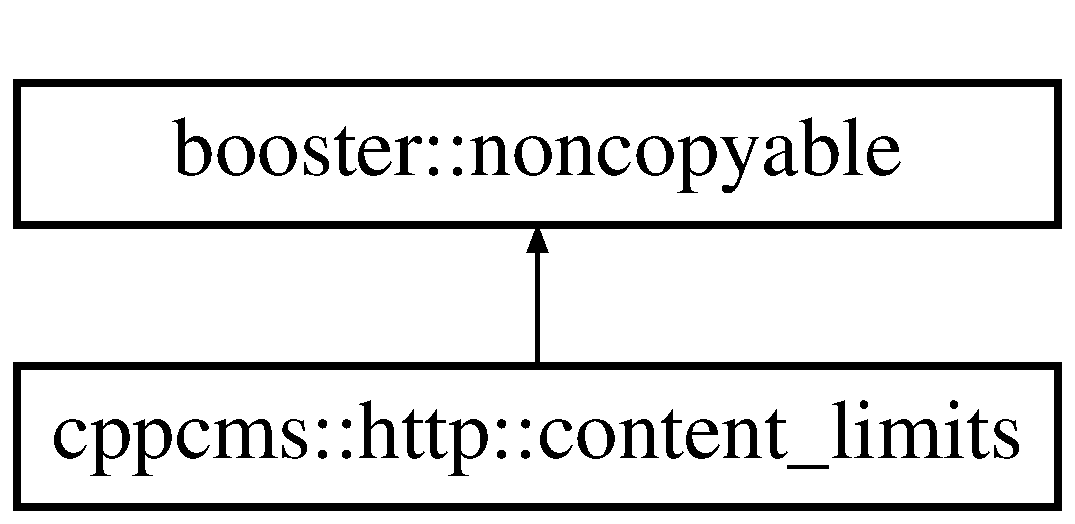
\includegraphics[height=2.000000cm]{classcppcms_1_1http_1_1content__limits}
\end{center}
\end{figure}
\subsection*{Public Member Functions}
\begin{DoxyCompactItemize}
\item 
long long {\bf content\+\_\+length\+\_\+limit} () const 
\item 
void {\bf content\+\_\+length\+\_\+limit} (long long size)
\item 
long long {\bf multipart\+\_\+form\+\_\+data\+\_\+limit} () const 
\item 
void {\bf multipart\+\_\+form\+\_\+data\+\_\+limit} (long long size)
\item 
size\+\_\+t {\bf file\+\_\+in\+\_\+memory\+\_\+limit} () const 
\item 
void {\bf file\+\_\+in\+\_\+memory\+\_\+limit} (size\+\_\+t size)
\item 
std\+::string {\bf uploads\+\_\+path} () const 
\item 
void {\bf uploads\+\_\+path} (std\+::string const \&path)
\end{DoxyCompactItemize}
\subsection*{Friends}
\begin{DoxyCompactItemize}
\item 
class {\bfseries request}\label{classcppcms_1_1http_1_1content__limits_a85b2d00ed5d8672f7dbb26f19a0b6123}

\end{DoxyCompactItemize}


\subsection{Detailed Description}
Class that represent the limits on the input content sizes

\doxyref{New in Cpp\+C\+MS 1.\+2}{p.}{v1_2} 

\subsection{Member Function Documentation}
\index{cppcms\+::http\+::content\+\_\+limits@{cppcms\+::http\+::content\+\_\+limits}!content\+\_\+length\+\_\+limit@{content\+\_\+length\+\_\+limit}}
\index{content\+\_\+length\+\_\+limit@{content\+\_\+length\+\_\+limit}!cppcms\+::http\+::content\+\_\+limits@{cppcms\+::http\+::content\+\_\+limits}}
\subsubsection[{content\+\_\+length\+\_\+limit() const }]{\setlength{\rightskip}{0pt plus 5cm}long long cppcms\+::http\+::content\+\_\+limits\+::content\+\_\+length\+\_\+limit (
\begin{DoxyParamCaption}
{}
\end{DoxyParamCaption}
) const}\label{classcppcms_1_1http_1_1content__limits_a21783c94b876ccaa7a00505911d82687}
Get the size limit in bytes of any non multipart/form-\/data content

Note form fields without content-\/type would be limited by this size even if the multipart\+\_\+form\+\_\+data\+\_\+limit is much larger \index{cppcms\+::http\+::content\+\_\+limits@{cppcms\+::http\+::content\+\_\+limits}!content\+\_\+length\+\_\+limit@{content\+\_\+length\+\_\+limit}}
\index{content\+\_\+length\+\_\+limit@{content\+\_\+length\+\_\+limit}!cppcms\+::http\+::content\+\_\+limits@{cppcms\+::http\+::content\+\_\+limits}}
\subsubsection[{content\+\_\+length\+\_\+limit(long long size)}]{\setlength{\rightskip}{0pt plus 5cm}void cppcms\+::http\+::content\+\_\+limits\+::content\+\_\+length\+\_\+limit (
\begin{DoxyParamCaption}
\item[{long long}]{size}
\end{DoxyParamCaption}
)}\label{classcppcms_1_1http_1_1content__limits_a9ed8f9a50eece6c1cb578fae23f2b885}
Set the size limit of any non multipart/form-\/data content

Note form fields without content-\/type would be limited by this size even if the multipart\+\_\+form\+\_\+data\+\_\+limit is much larger \index{cppcms\+::http\+::content\+\_\+limits@{cppcms\+::http\+::content\+\_\+limits}!file\+\_\+in\+\_\+memory\+\_\+limit@{file\+\_\+in\+\_\+memory\+\_\+limit}}
\index{file\+\_\+in\+\_\+memory\+\_\+limit@{file\+\_\+in\+\_\+memory\+\_\+limit}!cppcms\+::http\+::content\+\_\+limits@{cppcms\+::http\+::content\+\_\+limits}}
\subsubsection[{file\+\_\+in\+\_\+memory\+\_\+limit() const }]{\setlength{\rightskip}{0pt plus 5cm}size\+\_\+t cppcms\+::http\+::content\+\_\+limits\+::file\+\_\+in\+\_\+memory\+\_\+limit (
\begin{DoxyParamCaption}
{}
\end{DoxyParamCaption}
) const}\label{classcppcms_1_1http_1_1content__limits_add380bf850ba250ed84dad5843f620f0}
Get the maximal size of file that is still hold in memory rather than disk \index{cppcms\+::http\+::content\+\_\+limits@{cppcms\+::http\+::content\+\_\+limits}!file\+\_\+in\+\_\+memory\+\_\+limit@{file\+\_\+in\+\_\+memory\+\_\+limit}}
\index{file\+\_\+in\+\_\+memory\+\_\+limit@{file\+\_\+in\+\_\+memory\+\_\+limit}!cppcms\+::http\+::content\+\_\+limits@{cppcms\+::http\+::content\+\_\+limits}}
\subsubsection[{file\+\_\+in\+\_\+memory\+\_\+limit(size\+\_\+t size)}]{\setlength{\rightskip}{0pt plus 5cm}void cppcms\+::http\+::content\+\_\+limits\+::file\+\_\+in\+\_\+memory\+\_\+limit (
\begin{DoxyParamCaption}
\item[{size\+\_\+t}]{size}
\end{DoxyParamCaption}
)}\label{classcppcms_1_1http_1_1content__limits_acb17817c577d2c8712eb38a7595ea9f8}
Set the maximal size of file that is still hold in memory rather than disk \index{cppcms\+::http\+::content\+\_\+limits@{cppcms\+::http\+::content\+\_\+limits}!multipart\+\_\+form\+\_\+data\+\_\+limit@{multipart\+\_\+form\+\_\+data\+\_\+limit}}
\index{multipart\+\_\+form\+\_\+data\+\_\+limit@{multipart\+\_\+form\+\_\+data\+\_\+limit}!cppcms\+::http\+::content\+\_\+limits@{cppcms\+::http\+::content\+\_\+limits}}
\subsubsection[{multipart\+\_\+form\+\_\+data\+\_\+limit() const }]{\setlength{\rightskip}{0pt plus 5cm}long long cppcms\+::http\+::content\+\_\+limits\+::multipart\+\_\+form\+\_\+data\+\_\+limit (
\begin{DoxyParamCaption}
{}
\end{DoxyParamCaption}
) const}\label{classcppcms_1_1http_1_1content__limits_a1a0489bf5f0f22572976e53ce3b7fd9a}
Get the size limit of multipart/form-\/data content in bytes

Note form fields without content-\/type would be limited by content\+\_\+length\+\_\+limit size even if the multipart\+\_\+form\+\_\+data\+\_\+limit is much larger \index{cppcms\+::http\+::content\+\_\+limits@{cppcms\+::http\+::content\+\_\+limits}!multipart\+\_\+form\+\_\+data\+\_\+limit@{multipart\+\_\+form\+\_\+data\+\_\+limit}}
\index{multipart\+\_\+form\+\_\+data\+\_\+limit@{multipart\+\_\+form\+\_\+data\+\_\+limit}!cppcms\+::http\+::content\+\_\+limits@{cppcms\+::http\+::content\+\_\+limits}}
\subsubsection[{multipart\+\_\+form\+\_\+data\+\_\+limit(long long size)}]{\setlength{\rightskip}{0pt plus 5cm}void cppcms\+::http\+::content\+\_\+limits\+::multipart\+\_\+form\+\_\+data\+\_\+limit (
\begin{DoxyParamCaption}
\item[{long long}]{size}
\end{DoxyParamCaption}
)}\label{classcppcms_1_1http_1_1content__limits_a3f8e2dddb412689f463ef564dea675f4}
Set the size limit of multipart/form-\/data content in bytes

Note form fields without content-\/type would be limited by content\+\_\+length\+\_\+limit size even if the multipart\+\_\+form\+\_\+data\+\_\+limit is much larger \index{cppcms\+::http\+::content\+\_\+limits@{cppcms\+::http\+::content\+\_\+limits}!uploads\+\_\+path@{uploads\+\_\+path}}
\index{uploads\+\_\+path@{uploads\+\_\+path}!cppcms\+::http\+::content\+\_\+limits@{cppcms\+::http\+::content\+\_\+limits}}
\subsubsection[{uploads\+\_\+path() const }]{\setlength{\rightskip}{0pt plus 5cm}std\+::string cppcms\+::http\+::content\+\_\+limits\+::uploads\+\_\+path (
\begin{DoxyParamCaption}
{}
\end{DoxyParamCaption}
) const}\label{classcppcms_1_1http_1_1content__limits_a403550baf432d28e3a5a9da75270d9f5}
Get a location of a temporary directory that files are uploaded to, if empty system default is used \index{cppcms\+::http\+::content\+\_\+limits@{cppcms\+::http\+::content\+\_\+limits}!uploads\+\_\+path@{uploads\+\_\+path}}
\index{uploads\+\_\+path@{uploads\+\_\+path}!cppcms\+::http\+::content\+\_\+limits@{cppcms\+::http\+::content\+\_\+limits}}
\subsubsection[{uploads\+\_\+path(std\+::string const \&path)}]{\setlength{\rightskip}{0pt plus 5cm}void cppcms\+::http\+::content\+\_\+limits\+::uploads\+\_\+path (
\begin{DoxyParamCaption}
\item[{std\+::string const \&}]{path}
\end{DoxyParamCaption}
)}\label{classcppcms_1_1http_1_1content__limits_a074201a767722772bbd203cf9420e3f9}
Set a location of a temporary directory that files are uploaded to, if empty system default is used 

The documentation for this class was generated from the following file\+:\begin{DoxyCompactItemize}
\item 
cppcms/http\+\_\+content\+\_\+filter.\+h\end{DoxyCompactItemize}

\section{cppcms\+:\+:http\+:\+:content\+\_\+type Class Reference}
\label{classcppcms_1_1http_1_1content__type}\index{cppcms\+::http\+::content\+\_\+type@{cppcms\+::http\+::content\+\_\+type}}


Class that represents parsed Content-\/\+Type header, this is immutable class. Once it is created its values does not change.  




{\ttfamily \#include $<$cppcms/http\+\_\+content\+\_\+type.\+h$>$}

\subsection*{Public Member Functions}
\begin{DoxyCompactItemize}
\item 
std\+::string {\bf type} () const 
\item 
std\+::string {\bf subtype} () const 
\item 
std\+::string {\bf media\+\_\+type} () const 
\item 
std\+::string {\bf charset} () const 
\item 
std\+::map$<$ std\+::string, std\+::string $>$ {\bf parameters} () const 
\item 
std\+::string {\bf parameter\+\_\+by\+\_\+key} (std\+::string const \&key) const 
\item 
bool {\bf parameter\+\_\+is\+\_\+set} (std\+::string const \&key) const 
\item 
bool {\bf is\+\_\+form\+\_\+urlencoded} () const 
\item 
bool {\bf is\+\_\+multipart\+\_\+form\+\_\+data} () const 
\item 
{\bf content\+\_\+type} (std\+::string const \&ct)
\item 
{\bf content\+\_\+type} (char const $\ast$ct)
\item 
{\bf content\+\_\+type} (char const $\ast$begin, char const $\ast$end)
\item 
{\bf content\+\_\+type} ()
\item 
{\bf content\+\_\+type} ({\bf content\+\_\+type} const \&)
\item 
{\bf content\+\_\+type} const \& {\bf operator=} ({\bf content\+\_\+type} const \&)
\item 
{\bf $\sim$content\+\_\+type} ()
\item 
{\bf content\+\_\+type} ({\bf content\+\_\+type} \&\&)\label{classcppcms_1_1http_1_1content__type_a349be583cf2811367da3cc3427692ab7}

\begin{DoxyCompactList}\small\item\em Move ctor. \end{DoxyCompactList}\item 
{\bf content\+\_\+type} \& {\bf operator=} ({\bf content\+\_\+type} \&\&)\label{classcppcms_1_1http_1_1content__type_a77165ff23eb9aab35a66feca3d9444a2}

\begin{DoxyCompactList}\small\item\em Move =. \end{DoxyCompactList}\end{DoxyCompactItemize}


\subsection{Detailed Description}
Class that represents parsed Content-\/\+Type header, this is immutable class. Once it is created its values does not change. 

\subsection{Constructor \& Destructor Documentation}
\index{cppcms\+::http\+::content\+\_\+type@{cppcms\+::http\+::content\+\_\+type}!content\+\_\+type@{content\+\_\+type}}
\index{content\+\_\+type@{content\+\_\+type}!cppcms\+::http\+::content\+\_\+type@{cppcms\+::http\+::content\+\_\+type}}
\subsubsection[{content\+\_\+type(std\+::string const \&ct)}]{\setlength{\rightskip}{0pt plus 5cm}cppcms\+::http\+::content\+\_\+type\+::content\+\_\+type (
\begin{DoxyParamCaption}
\item[{std\+::string const \&}]{ct}
\end{DoxyParamCaption}
)}\label{classcppcms_1_1http_1_1content__type_a8ca32018b9f26d6d36d01644325bc1be}
Parse content type {\itshape ct} and create the class \index{cppcms\+::http\+::content\+\_\+type@{cppcms\+::http\+::content\+\_\+type}!content\+\_\+type@{content\+\_\+type}}
\index{content\+\_\+type@{content\+\_\+type}!cppcms\+::http\+::content\+\_\+type@{cppcms\+::http\+::content\+\_\+type}}
\subsubsection[{content\+\_\+type(char const $\ast$ct)}]{\setlength{\rightskip}{0pt plus 5cm}cppcms\+::http\+::content\+\_\+type\+::content\+\_\+type (
\begin{DoxyParamCaption}
\item[{char const $\ast$}]{ct}
\end{DoxyParamCaption}
)}\label{classcppcms_1_1http_1_1content__type_a432f9bf9ac47a98c77c3db61ccab897c}
Parse content type {\itshape ct} and create the class \index{cppcms\+::http\+::content\+\_\+type@{cppcms\+::http\+::content\+\_\+type}!content\+\_\+type@{content\+\_\+type}}
\index{content\+\_\+type@{content\+\_\+type}!cppcms\+::http\+::content\+\_\+type@{cppcms\+::http\+::content\+\_\+type}}
\subsubsection[{content\+\_\+type(char const $\ast$begin, char const $\ast$end)}]{\setlength{\rightskip}{0pt plus 5cm}cppcms\+::http\+::content\+\_\+type\+::content\+\_\+type (
\begin{DoxyParamCaption}
\item[{char const $\ast$}]{begin, }
\item[{char const $\ast$}]{end}
\end{DoxyParamCaption}
)}\label{classcppcms_1_1http_1_1content__type_aab6c2029cd156f3ca473ebabbbcabcc6}
Parse content type in range [begin,end) and create the class \index{cppcms\+::http\+::content\+\_\+type@{cppcms\+::http\+::content\+\_\+type}!content\+\_\+type@{content\+\_\+type}}
\index{content\+\_\+type@{content\+\_\+type}!cppcms\+::http\+::content\+\_\+type@{cppcms\+::http\+::content\+\_\+type}}
\subsubsection[{content\+\_\+type()}]{\setlength{\rightskip}{0pt plus 5cm}cppcms\+::http\+::content\+\_\+type\+::content\+\_\+type (
\begin{DoxyParamCaption}
{}
\end{DoxyParamCaption}
)}\label{classcppcms_1_1http_1_1content__type_ac0a5db595e4e3aafed2c01d693678c02}
Empty one... \index{cppcms\+::http\+::content\+\_\+type@{cppcms\+::http\+::content\+\_\+type}!content\+\_\+type@{content\+\_\+type}}
\index{content\+\_\+type@{content\+\_\+type}!cppcms\+::http\+::content\+\_\+type@{cppcms\+::http\+::content\+\_\+type}}
\subsubsection[{content\+\_\+type(content\+\_\+type const \&)}]{\setlength{\rightskip}{0pt plus 5cm}cppcms\+::http\+::content\+\_\+type\+::content\+\_\+type (
\begin{DoxyParamCaption}
\item[{{\bf content\+\_\+type} const \&}]{}
\end{DoxyParamCaption}
)}\label{classcppcms_1_1http_1_1content__type_a83798fd889f5949a3476424213fa3bf8}
Copy constructor \index{cppcms\+::http\+::content\+\_\+type@{cppcms\+::http\+::content\+\_\+type}!````~content\+\_\+type@{$\sim$content\+\_\+type}}
\index{````~content\+\_\+type@{$\sim$content\+\_\+type}!cppcms\+::http\+::content\+\_\+type@{cppcms\+::http\+::content\+\_\+type}}
\subsubsection[{$\sim$content\+\_\+type()}]{\setlength{\rightskip}{0pt plus 5cm}cppcms\+::http\+::content\+\_\+type\+::$\sim$content\+\_\+type (
\begin{DoxyParamCaption}
{}
\end{DoxyParamCaption}
)}\label{classcppcms_1_1http_1_1content__type_a3cfc56a4071faeef2dfba42b324d169f}
Destructor 

\subsection{Member Function Documentation}
\index{cppcms\+::http\+::content\+\_\+type@{cppcms\+::http\+::content\+\_\+type}!charset@{charset}}
\index{charset@{charset}!cppcms\+::http\+::content\+\_\+type@{cppcms\+::http\+::content\+\_\+type}}
\subsubsection[{charset() const }]{\setlength{\rightskip}{0pt plus 5cm}std\+::string cppcms\+::http\+::content\+\_\+type\+::charset (
\begin{DoxyParamCaption}
{}
\end{DoxyParamCaption}
) const}\label{classcppcms_1_1http_1_1content__type_a265c09ef5ae8c82c7371398011b55de5}
Charset parameter, if given, for example, for \char`\"{}text/html; charset=\+U\+T\+F-\/8\char`\"{} it would be \char`\"{}\+U\+T\+F-\/8\char`\"{}. If charset is not specified, it would return an empty string \index{cppcms\+::http\+::content\+\_\+type@{cppcms\+::http\+::content\+\_\+type}!is\+\_\+form\+\_\+urlencoded@{is\+\_\+form\+\_\+urlencoded}}
\index{is\+\_\+form\+\_\+urlencoded@{is\+\_\+form\+\_\+urlencoded}!cppcms\+::http\+::content\+\_\+type@{cppcms\+::http\+::content\+\_\+type}}
\subsubsection[{is\+\_\+form\+\_\+urlencoded() const }]{\setlength{\rightskip}{0pt plus 5cm}bool cppcms\+::http\+::content\+\_\+type\+::is\+\_\+form\+\_\+urlencoded (
\begin{DoxyParamCaption}
{}
\end{DoxyParamCaption}
) const}\label{classcppcms_1_1http_1_1content__type_a32ef0b0e19c3454157f58d2fc556bcf2}
Check if media type application/x-\/www-\/form-\/urlencoded \doxyref{content\+\_\+type}{p.}{classcppcms_1_1http_1_1content__type}

\doxyref{New in Cpp\+C\+MS 1.\+2}{p.}{v1_2} \index{cppcms\+::http\+::content\+\_\+type@{cppcms\+::http\+::content\+\_\+type}!is\+\_\+multipart\+\_\+form\+\_\+data@{is\+\_\+multipart\+\_\+form\+\_\+data}}
\index{is\+\_\+multipart\+\_\+form\+\_\+data@{is\+\_\+multipart\+\_\+form\+\_\+data}!cppcms\+::http\+::content\+\_\+type@{cppcms\+::http\+::content\+\_\+type}}
\subsubsection[{is\+\_\+multipart\+\_\+form\+\_\+data() const }]{\setlength{\rightskip}{0pt plus 5cm}bool cppcms\+::http\+::content\+\_\+type\+::is\+\_\+multipart\+\_\+form\+\_\+data (
\begin{DoxyParamCaption}
{}
\end{DoxyParamCaption}
) const}\label{classcppcms_1_1http_1_1content__type_ac760c57bde9ecab5056365526ef06d50}
Check if media type is multipart/form-\/data \doxyref{content\+\_\+type}{p.}{classcppcms_1_1http_1_1content__type}

\doxyref{New in Cpp\+C\+MS 1.\+2}{p.}{v1_2} \index{cppcms\+::http\+::content\+\_\+type@{cppcms\+::http\+::content\+\_\+type}!media\+\_\+type@{media\+\_\+type}}
\index{media\+\_\+type@{media\+\_\+type}!cppcms\+::http\+::content\+\_\+type@{cppcms\+::http\+::content\+\_\+type}}
\subsubsection[{media\+\_\+type() const }]{\setlength{\rightskip}{0pt plus 5cm}std\+::string cppcms\+::http\+::content\+\_\+type\+::media\+\_\+type (
\begin{DoxyParamCaption}
{}
\end{DoxyParamCaption}
) const}\label{classcppcms_1_1http_1_1content__type_a67114242a60b8cab2787ad97f2104fba}
The full media type of content type, for example, for \char`\"{}text/html; charset=\+U\+T\+F-\/8\char`\"{} it would be \char`\"{}text/html\char`\"{} in lower case \index{cppcms\+::http\+::content\+\_\+type@{cppcms\+::http\+::content\+\_\+type}!operator=@{operator=}}
\index{operator=@{operator=}!cppcms\+::http\+::content\+\_\+type@{cppcms\+::http\+::content\+\_\+type}}
\subsubsection[{operator=(content\+\_\+type const \&)}]{\setlength{\rightskip}{0pt plus 5cm}{\bf content\+\_\+type} const\& cppcms\+::http\+::content\+\_\+type\+::operator= (
\begin{DoxyParamCaption}
\item[{{\bf content\+\_\+type} const \&}]{}
\end{DoxyParamCaption}
)}\label{classcppcms_1_1http_1_1content__type_a075af9ec4d38104d069da618a8ec6c4e}
Assignment operator \index{cppcms\+::http\+::content\+\_\+type@{cppcms\+::http\+::content\+\_\+type}!parameter\+\_\+by\+\_\+key@{parameter\+\_\+by\+\_\+key}}
\index{parameter\+\_\+by\+\_\+key@{parameter\+\_\+by\+\_\+key}!cppcms\+::http\+::content\+\_\+type@{cppcms\+::http\+::content\+\_\+type}}
\subsubsection[{parameter\+\_\+by\+\_\+key(std\+::string const \&key) const }]{\setlength{\rightskip}{0pt plus 5cm}std\+::string cppcms\+::http\+::content\+\_\+type\+::parameter\+\_\+by\+\_\+key (
\begin{DoxyParamCaption}
\item[{std\+::string const \&}]{key}
\end{DoxyParamCaption}
) const}\label{classcppcms_1_1http_1_1content__type_a84436875c61d1da495dc2d2961f3539d}
Get parameter\textquotesingle{}s value by key (should be in lowercase), returns empty string if not set \index{cppcms\+::http\+::content\+\_\+type@{cppcms\+::http\+::content\+\_\+type}!parameter\+\_\+is\+\_\+set@{parameter\+\_\+is\+\_\+set}}
\index{parameter\+\_\+is\+\_\+set@{parameter\+\_\+is\+\_\+set}!cppcms\+::http\+::content\+\_\+type@{cppcms\+::http\+::content\+\_\+type}}
\subsubsection[{parameter\+\_\+is\+\_\+set(std\+::string const \&key) const }]{\setlength{\rightskip}{0pt plus 5cm}bool cppcms\+::http\+::content\+\_\+type\+::parameter\+\_\+is\+\_\+set (
\begin{DoxyParamCaption}
\item[{std\+::string const \&}]{key}
\end{DoxyParamCaption}
) const}\label{classcppcms_1_1http_1_1content__type_a8b26f1daf90f5d45067bb96ee1782c64}
Check if the parameter is set using key (should be in lowercase) \index{cppcms\+::http\+::content\+\_\+type@{cppcms\+::http\+::content\+\_\+type}!parameters@{parameters}}
\index{parameters@{parameters}!cppcms\+::http\+::content\+\_\+type@{cppcms\+::http\+::content\+\_\+type}}
\subsubsection[{parameters() const }]{\setlength{\rightskip}{0pt plus 5cm}std\+::map$<$std\+::string,std\+::string$>$ cppcms\+::http\+::content\+\_\+type\+::parameters (
\begin{DoxyParamCaption}
{}
\end{DoxyParamCaption}
) const}\label{classcppcms_1_1http_1_1content__type_ac79a6ec633d805a1b479c6ccd8c1dc20}
All parameters, all parameter keys are in lower case, the values are given as is. \index{cppcms\+::http\+::content\+\_\+type@{cppcms\+::http\+::content\+\_\+type}!subtype@{subtype}}
\index{subtype@{subtype}!cppcms\+::http\+::content\+\_\+type@{cppcms\+::http\+::content\+\_\+type}}
\subsubsection[{subtype() const }]{\setlength{\rightskip}{0pt plus 5cm}std\+::string cppcms\+::http\+::content\+\_\+type\+::subtype (
\begin{DoxyParamCaption}
{}
\end{DoxyParamCaption}
) const}\label{classcppcms_1_1http_1_1content__type_a98f4bdf669f9511c5b0acddf113eba6d}
The subtype part of content type, for example, for \char`\"{}text/html; charset=\+U\+T\+F-\/8\char`\"{} it would be \char`\"{}html\char`\"{} in lower case \index{cppcms\+::http\+::content\+\_\+type@{cppcms\+::http\+::content\+\_\+type}!type@{type}}
\index{type@{type}!cppcms\+::http\+::content\+\_\+type@{cppcms\+::http\+::content\+\_\+type}}
\subsubsection[{type() const }]{\setlength{\rightskip}{0pt plus 5cm}std\+::string cppcms\+::http\+::content\+\_\+type\+::type (
\begin{DoxyParamCaption}
{}
\end{DoxyParamCaption}
) const}\label{classcppcms_1_1http_1_1content__type_a77fd1a4dc12b840e952bd28e1761b5fa}
The type part of content type, for example, for \char`\"{}text/html; charset=\+U\+T\+F-\/8\char`\"{} it would be \char`\"{}text\char`\"{} in lower case 

The documentation for this class was generated from the following file\+:\begin{DoxyCompactItemize}
\item 
cppcms/http\+\_\+content\+\_\+type.\+h\end{DoxyCompactItemize}

\section{cppcms\+:\+:http\+:\+:context Class Reference}
\label{classcppcms_1_1http_1_1context}\index{cppcms\+::http\+::context@{cppcms\+::http\+::context}}


context is a central class that holds all specific connection related information. It encapsulates C\+GI request and response, cache, session and locale information  




{\ttfamily \#include $<$cppcms/http\+\_\+context.\+h$>$}

Inheritance diagram for cppcms\+:\+:http\+:\+:context\+:\begin{figure}[H]
\begin{center}
\leavevmode
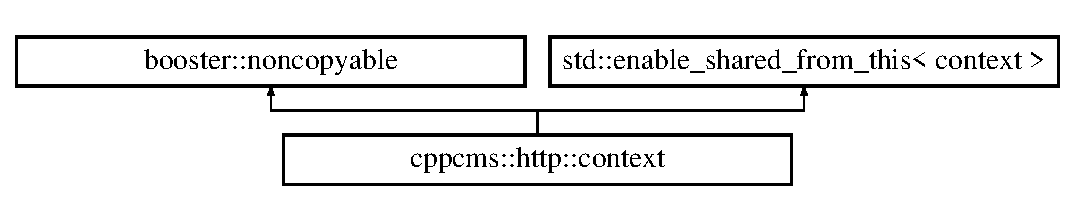
\includegraphics[height=2.000000cm]{classcppcms_1_1http_1_1context}
\end{center}
\end{figure}
\subsection*{Public Types}
\begin{DoxyCompactItemize}
\item 
enum {\bf completion\+\_\+type} \{ {\bf operation\+\_\+completed}, 
{\bf operation\+\_\+aborted}
 \}
\item 
typedef {\bf booster\+::callback}$<$ void({\bf completion\+\_\+type})$>$ {\bfseries handler}\label{classcppcms_1_1http_1_1context_af6f3005eb3252b98df96f87878e41560}

\end{DoxyCompactItemize}
\subsection*{Public Member Functions}
\begin{DoxyCompactItemize}
\item 
{\bf http\+::request} \& {\bf request} ()
\item 
{\bf http\+::response} \& {\bf response} ()
\item 
{\bf json\+::value} const \& {\bf settings} ()
\item 
{\bf cache\+\_\+interface} \& {\bf cache} ()
\item 
{\bf session\+\_\+interface} \& {\bf session} ()
\item 
std\+::locale {\bf locale} ()
\item 
void {\bf locale} (std\+::locale const \&new\+\_\+locale)
\item 
void {\bf locale} (std\+::string const \&name)
\item 
{\bf cppcms\+::service} \& {\bf service} ()
\item 
std\+::string {\bf skin} ()
\item 
void {\bf skin} (std\+::string const \&name)
\item 
void {\bf complete\+\_\+response} ()
\item 
void {\bf async\+\_\+complete\+\_\+response} ()
\item 
void {\bf async\+\_\+flush\+\_\+output} ({\bf handler} const \&h)
\item 
void {\bf async\+\_\+on\+\_\+peer\+\_\+reset} ({\bf booster\+::callback}$<$ void()$>$ const \&h)
\item 
void {\bf submit\+\_\+to\+\_\+pool} (booster\+::shared\+\_\+ptr$<$ {\bf application\+\_\+specific\+\_\+pool} $>$ pool, std\+::string const \&matched\+\_\+url)
\item 
void {\bf submit\+\_\+to\+\_\+asynchronous\+\_\+application} ({\bf booster\+::intrusive\+\_\+ptr}$<$ {\bf application} $>$ app, std\+::string const \&matched\+\_\+url)
\item 
{\footnotesize template$<$typename T $>$ }\\T $\ast$ {\bf get\+\_\+specific} ()
\item 
{\footnotesize template$<$typename T $>$ }\\void {\bf reset\+\_\+specific} (T $\ast$ptr=0)
\item 
{\footnotesize template$<$typename T $>$ }\\T $\ast$ {\bf release\+\_\+specific} ()
\end{DoxyCompactItemize}
\subsection*{Friends}
\begin{DoxyCompactItemize}
\item 
class {\bfseries impl\+::cgi\+::connection}\label{classcppcms_1_1http_1_1context_a35a6637347117934569e84977b6f5143}

\end{DoxyCompactItemize}


\subsection{Detailed Description}
context is a central class that holds all specific connection related information. It encapsulates C\+GI request and response, cache, session and locale information 

Instance of this class is created upon client requests, it provides access to all connection related interfaces. This class is unique per each applications hierarchy and destroyed when H\+T\+TP request/response is completed 

\subsection{Member Enumeration Documentation}
\index{cppcms\+::http\+::context@{cppcms\+::http\+::context}!completion\+\_\+type@{completion\+\_\+type}}
\index{completion\+\_\+type@{completion\+\_\+type}!cppcms\+::http\+::context@{cppcms\+::http\+::context}}
\subsubsection[{completion\+\_\+type}]{\setlength{\rightskip}{0pt plus 5cm}enum {\bf cppcms\+::http\+::context\+::completion\+\_\+type}}\label{classcppcms_1_1http_1_1context_a826eb2e00a4d0ad73cfc6b0100c0d06f}
\begin{Desc}
\item[Enumerator]\par
\begin{description}
\index{operation\+\_\+completed@{operation\+\_\+completed}!cppcms\+::http\+::context@{cppcms\+::http\+::context}}\index{cppcms\+::http\+::context@{cppcms\+::http\+::context}!operation\+\_\+completed@{operation\+\_\+completed}}\item[{\em 
operation\+\_\+completed\label{classcppcms_1_1http_1_1context_a826eb2e00a4d0ad73cfc6b0100c0d06faa16dd3b6428f001023d759aa96bbfcd7}
}]Asynchronous operation completed successfully. \index{operation\+\_\+aborted@{operation\+\_\+aborted}!cppcms\+::http\+::context@{cppcms\+::http\+::context}}\index{cppcms\+::http\+::context@{cppcms\+::http\+::context}!operation\+\_\+aborted@{operation\+\_\+aborted}}\item[{\em 
operation\+\_\+aborted\label{classcppcms_1_1http_1_1context_a826eb2e00a4d0ad73cfc6b0100c0d06fa83b1e94e0179a4f4c9597350fadb104f}
}]Asynchronous operation was canceled. \end{description}
\end{Desc}


\subsection{Member Function Documentation}
\index{cppcms\+::http\+::context@{cppcms\+::http\+::context}!async\+\_\+complete\+\_\+response@{async\+\_\+complete\+\_\+response}}
\index{async\+\_\+complete\+\_\+response@{async\+\_\+complete\+\_\+response}!cppcms\+::http\+::context@{cppcms\+::http\+::context}}
\subsubsection[{async\+\_\+complete\+\_\+response()}]{\setlength{\rightskip}{0pt plus 5cm}void cppcms\+::http\+::context\+::async\+\_\+complete\+\_\+response (
\begin{DoxyParamCaption}
{}
\end{DoxyParamCaption}
)}\label{classcppcms_1_1http_1_1context_a6d2c2128114b2c9f8cffd0bfe96dcd94}
Send all pending output data to the client and finalize the connection. Note, you can\textquotesingle{}t use this object for communication any more. \index{cppcms\+::http\+::context@{cppcms\+::http\+::context}!async\+\_\+flush\+\_\+output@{async\+\_\+flush\+\_\+output}}
\index{async\+\_\+flush\+\_\+output@{async\+\_\+flush\+\_\+output}!cppcms\+::http\+::context@{cppcms\+::http\+::context}}
\subsubsection[{async\+\_\+flush\+\_\+output(handler const \&h)}]{\setlength{\rightskip}{0pt plus 5cm}void cppcms\+::http\+::context\+::async\+\_\+flush\+\_\+output (
\begin{DoxyParamCaption}
\item[{{\bf handler} const \&}]{h}
\end{DoxyParamCaption}
)}\label{classcppcms_1_1http_1_1context_a134469b5dc46667596c360b8b7284dff}
Send all pending data to user, when operation is complete call handler {\itshape h} with status.

Note\+: if the status is operation\+\_\+aborted, you can\textquotesingle{}t use this connection any more, the peer gone. \index{cppcms\+::http\+::context@{cppcms\+::http\+::context}!async\+\_\+on\+\_\+peer\+\_\+reset@{async\+\_\+on\+\_\+peer\+\_\+reset}}
\index{async\+\_\+on\+\_\+peer\+\_\+reset@{async\+\_\+on\+\_\+peer\+\_\+reset}!cppcms\+::http\+::context@{cppcms\+::http\+::context}}
\subsubsection[{async\+\_\+on\+\_\+peer\+\_\+reset(booster\+::callback$<$ void()$>$ const \&h)}]{\setlength{\rightskip}{0pt plus 5cm}void cppcms\+::http\+::context\+::async\+\_\+on\+\_\+peer\+\_\+reset (
\begin{DoxyParamCaption}
\item[{{\bf booster\+::callback}$<$ void()$>$ const \&}]{h}
\end{DoxyParamCaption}
)}\label{classcppcms_1_1http_1_1context_a0f6fe53deabd90fee0ced81a8df6404e}
Set handler for peer reset events. It is useful to cleanup connections that had timeout or just disconnected by user

Notes\+:


\begin{DoxyEnumerate}
\item if async\+\_\+complete\+\_\+response was called, handler would not be called any more.
\item If async\+\_\+flush\+\_\+output fails, this does not mean that this handler would be called as well, so you need to check both 
\end{DoxyEnumerate}\index{cppcms\+::http\+::context@{cppcms\+::http\+::context}!cache@{cache}}
\index{cache@{cache}!cppcms\+::http\+::context@{cppcms\+::http\+::context}}
\subsubsection[{cache()}]{\setlength{\rightskip}{0pt plus 5cm}{\bf cache\+\_\+interface}\& cppcms\+::http\+::context\+::cache (
\begin{DoxyParamCaption}
{}
\end{DoxyParamCaption}
)}\label{classcppcms_1_1http_1_1context_a03a1a9094f04c6a14d66cb320d8b7ed0}
Get an interface to Cpp\+C\+MS Cache \index{cppcms\+::http\+::context@{cppcms\+::http\+::context}!complete\+\_\+response@{complete\+\_\+response}}
\index{complete\+\_\+response@{complete\+\_\+response}!cppcms\+::http\+::context@{cppcms\+::http\+::context}}
\subsubsection[{complete\+\_\+response()}]{\setlength{\rightskip}{0pt plus 5cm}void cppcms\+::http\+::context\+::complete\+\_\+response (
\begin{DoxyParamCaption}
{}
\end{DoxyParamCaption}
)}\label{classcppcms_1_1http_1_1context_a073981554e99770a9f082eaa90af1bd9}
Send all pending output data to the client and finalize the connection. Note, you can\textquotesingle{}t use this object for communication any more. \index{cppcms\+::http\+::context@{cppcms\+::http\+::context}!get\+\_\+specific@{get\+\_\+specific}}
\index{get\+\_\+specific@{get\+\_\+specific}!cppcms\+::http\+::context@{cppcms\+::http\+::context}}
\subsubsection[{get\+\_\+specific()}]{\setlength{\rightskip}{0pt plus 5cm}template$<$typename T $>$ T$\ast$ cppcms\+::http\+::context\+::get\+\_\+specific (
\begin{DoxyParamCaption}
{}
\end{DoxyParamCaption}
)\hspace{0.3cm}{\ttfamily [inline]}}\label{classcppcms_1_1http_1_1context_ad94dd7968efd8efdc24d177500cfc8d8}
Get context specific value of type T binded to context. If none is stored or type mismatched N\+U\+LL is returned

\doxyref{New in Cpp\+C\+MS 1.\+2}{p.}{v1_2} \index{cppcms\+::http\+::context@{cppcms\+::http\+::context}!locale@{locale}}
\index{locale@{locale}!cppcms\+::http\+::context@{cppcms\+::http\+::context}}
\subsubsection[{locale()}]{\setlength{\rightskip}{0pt plus 5cm}std\+::locale cppcms\+::http\+::context\+::locale (
\begin{DoxyParamCaption}
{}
\end{DoxyParamCaption}
)}\label{classcppcms_1_1http_1_1context_a39fde738210daf84deee691f45260e5b}
Get current context locale 

Referenced by cppcms\+::widgets\+::numeric$<$ T $>$\+::load().

\index{cppcms\+::http\+::context@{cppcms\+::http\+::context}!locale@{locale}}
\index{locale@{locale}!cppcms\+::http\+::context@{cppcms\+::http\+::context}}
\subsubsection[{locale(std\+::locale const \&new\+\_\+locale)}]{\setlength{\rightskip}{0pt plus 5cm}void cppcms\+::http\+::context\+::locale (
\begin{DoxyParamCaption}
\item[{std\+::locale const \&}]{new\+\_\+locale}
\end{DoxyParamCaption}
)}\label{classcppcms_1_1http_1_1context_a9d6ee6ce1d9007ba1c0d7222fa022fd8}
Set locale explicitly. Note, it changes the locale of the \doxyref{response()}{p.}{classcppcms_1_1http_1_1context_ac470c44432f9570e227330e974630872}.out() stream as well \index{cppcms\+::http\+::context@{cppcms\+::http\+::context}!locale@{locale}}
\index{locale@{locale}!cppcms\+::http\+::context@{cppcms\+::http\+::context}}
\subsubsection[{locale(std\+::string const \&name)}]{\setlength{\rightskip}{0pt plus 5cm}void cppcms\+::http\+::context\+::locale (
\begin{DoxyParamCaption}
\item[{std\+::string const \&}]{name}
\end{DoxyParamCaption}
)}\label{classcppcms_1_1http_1_1context_a036d52a76868c0736716b19e32b602a3}
Set locale by name. Similar to locale(\doxyref{service()}{p.}{classcppcms_1_1http_1_1context_a30c62fea3de87dabd6580f2257599a49}.generator(name)).

Note\+: it changes the locale of the \doxyref{response()}{p.}{classcppcms_1_1http_1_1context_ac470c44432f9570e227330e974630872}.out() stream as well \index{cppcms\+::http\+::context@{cppcms\+::http\+::context}!release\+\_\+specific@{release\+\_\+specific}}
\index{release\+\_\+specific@{release\+\_\+specific}!cppcms\+::http\+::context@{cppcms\+::http\+::context}}
\subsubsection[{release\+\_\+specific()}]{\setlength{\rightskip}{0pt plus 5cm}template$<$typename T $>$ T$\ast$ cppcms\+::http\+::context\+::release\+\_\+specific (
\begin{DoxyParamCaption}
{}
\end{DoxyParamCaption}
)\hspace{0.3cm}{\ttfamily [inline]}}\label{classcppcms_1_1http_1_1context_ad78ceacb71f189560bf53e98ce8ceddb}
Release context specific value binded to context.

\doxyref{New in Cpp\+C\+MS 1.\+2}{p.}{v1_2} \index{cppcms\+::http\+::context@{cppcms\+::http\+::context}!request@{request}}
\index{request@{request}!cppcms\+::http\+::context@{cppcms\+::http\+::context}}
\subsubsection[{request()}]{\setlength{\rightskip}{0pt plus 5cm}{\bf http\+::request}\& cppcms\+::http\+::context\+::request (
\begin{DoxyParamCaption}
{}
\end{DoxyParamCaption}
)}\label{classcppcms_1_1http_1_1context_a79f5c6ad0f4dca64256abb0809d40cba}
Get an interface to H\+T\+TP request 

Referenced by cppcms\+::widgets\+::numeric$<$ T $>$\+::load().

\index{cppcms\+::http\+::context@{cppcms\+::http\+::context}!reset\+\_\+specific@{reset\+\_\+specific}}
\index{reset\+\_\+specific@{reset\+\_\+specific}!cppcms\+::http\+::context@{cppcms\+::http\+::context}}
\subsubsection[{reset\+\_\+specific(\+T $\ast$ptr=0)}]{\setlength{\rightskip}{0pt plus 5cm}template$<$typename T $>$ void cppcms\+::http\+::context\+::reset\+\_\+specific (
\begin{DoxyParamCaption}
\item[{T $\ast$}]{ptr = {\ttfamily 0}}
\end{DoxyParamCaption}
)\hspace{0.3cm}{\ttfamily [inline]}}\label{classcppcms_1_1http_1_1context_a9ade01f327999cebf9f0f5a28fb7e9d8}
Reset context specific value of type T binded to context. Old value is deleted

\doxyref{New in Cpp\+C\+MS 1.\+2}{p.}{v1_2} \index{cppcms\+::http\+::context@{cppcms\+::http\+::context}!response@{response}}
\index{response@{response}!cppcms\+::http\+::context@{cppcms\+::http\+::context}}
\subsubsection[{response()}]{\setlength{\rightskip}{0pt plus 5cm}{\bf http\+::response}\& cppcms\+::http\+::context\+::response (
\begin{DoxyParamCaption}
{}
\end{DoxyParamCaption}
)}\label{classcppcms_1_1http_1_1context_ac470c44432f9570e227330e974630872}
Get an interface to H\+T\+TP response \index{cppcms\+::http\+::context@{cppcms\+::http\+::context}!service@{service}}
\index{service@{service}!cppcms\+::http\+::context@{cppcms\+::http\+::context}}
\subsubsection[{service()}]{\setlength{\rightskip}{0pt plus 5cm}{\bf cppcms\+::service}\& cppcms\+::http\+::context\+::service (
\begin{DoxyParamCaption}
{}
\end{DoxyParamCaption}
)}\label{classcppcms_1_1http_1_1context_a30c62fea3de87dabd6580f2257599a49}
Get the central service instance \index{cppcms\+::http\+::context@{cppcms\+::http\+::context}!session@{session}}
\index{session@{session}!cppcms\+::http\+::context@{cppcms\+::http\+::context}}
\subsubsection[{session()}]{\setlength{\rightskip}{0pt plus 5cm}{\bf session\+\_\+interface}\& cppcms\+::http\+::context\+::session (
\begin{DoxyParamCaption}
{}
\end{DoxyParamCaption}
)}\label{classcppcms_1_1http_1_1context_abb47ca8cc18020efe394d26f590b6f97}
Get an interface to current session

Note, when using asynchronous Cpp\+C\+MS applications, session data is not fetched and is not updated, because session access may be not cheap, So when using \doxyref{session\+\_\+interface}{p.}{classcppcms_1_1session__interface} in asynchronous application make sure you call session\+\_\+inerface\+::load member function \index{cppcms\+::http\+::context@{cppcms\+::http\+::context}!settings@{settings}}
\index{settings@{settings}!cppcms\+::http\+::context@{cppcms\+::http\+::context}}
\subsubsection[{settings()}]{\setlength{\rightskip}{0pt plus 5cm}{\bf json\+::value} const\& cppcms\+::http\+::context\+::settings (
\begin{DoxyParamCaption}
{}
\end{DoxyParamCaption}
)}\label{classcppcms_1_1http_1_1context_a3cd9ff89c81ae29259cbacbee2749fb4}
Get global settings. Same as \doxyref{cppcms\+::service\+::settings}{p.}{classcppcms_1_1service_a2655891c41745defac52587b4ecae53b} \index{cppcms\+::http\+::context@{cppcms\+::http\+::context}!skin@{skin}}
\index{skin@{skin}!cppcms\+::http\+::context@{cppcms\+::http\+::context}}
\subsubsection[{skin()}]{\setlength{\rightskip}{0pt plus 5cm}std\+::string cppcms\+::http\+::context\+::skin (
\begin{DoxyParamCaption}
{}
\end{DoxyParamCaption}
)}\label{classcppcms_1_1http_1_1context_ad6d98b1577946314257b7b9cbef1776c}
Get current views skin name \index{cppcms\+::http\+::context@{cppcms\+::http\+::context}!skin@{skin}}
\index{skin@{skin}!cppcms\+::http\+::context@{cppcms\+::http\+::context}}
\subsubsection[{skin(std\+::string const \&name)}]{\setlength{\rightskip}{0pt plus 5cm}void cppcms\+::http\+::context\+::skin (
\begin{DoxyParamCaption}
\item[{std\+::string const \&}]{name}
\end{DoxyParamCaption}
)}\label{classcppcms_1_1http_1_1context_af1230c69d6824e220e0fcd35b29118bc}
Set current views skin name \index{cppcms\+::http\+::context@{cppcms\+::http\+::context}!submit\+\_\+to\+\_\+asynchronous\+\_\+application@{submit\+\_\+to\+\_\+asynchronous\+\_\+application}}
\index{submit\+\_\+to\+\_\+asynchronous\+\_\+application@{submit\+\_\+to\+\_\+asynchronous\+\_\+application}!cppcms\+::http\+::context@{cppcms\+::http\+::context}}
\subsubsection[{submit\+\_\+to\+\_\+asynchronous\+\_\+application(booster\+::intrusive\+\_\+ptr$<$ application $>$ app, std\+::string const \&matched\+\_\+url)}]{\setlength{\rightskip}{0pt plus 5cm}void cppcms\+::http\+::context\+::submit\+\_\+to\+\_\+asynchronous\+\_\+application (
\begin{DoxyParamCaption}
\item[{{\bf booster\+::intrusive\+\_\+ptr}$<$ {\bf application} $>$}]{app, }
\item[{std\+::string const \&}]{matched\+\_\+url}
\end{DoxyParamCaption}
)}\label{classcppcms_1_1http_1_1context_a317a093fabaebc36ac31afdf98c17ba7}
Submit the context to alternative application -\/ allows to transfer context from application to application, {\itshape matched\+\_\+url} would be given to \doxyref{application\+::main}{p.}{classcppcms_1_1application_a8c884a9309d107237e8946446feba8f8} for processing

Note\+:


\begin{DoxyItemize}
\item the app should be asynchronous
\item no output should be itransfered on this context
\item the context M\+U\+ST be detached for existing application
\end{DoxyItemize}

This function can be called from any thread

\doxyref{New in Cpp\+C\+MS 1.\+2}{p.}{v1_2} \index{cppcms\+::http\+::context@{cppcms\+::http\+::context}!submit\+\_\+to\+\_\+pool@{submit\+\_\+to\+\_\+pool}}
\index{submit\+\_\+to\+\_\+pool@{submit\+\_\+to\+\_\+pool}!cppcms\+::http\+::context@{cppcms\+::http\+::context}}
\subsubsection[{submit\+\_\+to\+\_\+pool(booster\+::shared\+\_\+ptr$<$ application\+\_\+specific\+\_\+pool $>$ pool, std\+::string const \&matched\+\_\+url)}]{\setlength{\rightskip}{0pt plus 5cm}void cppcms\+::http\+::context\+::submit\+\_\+to\+\_\+pool (
\begin{DoxyParamCaption}
\item[{booster\+::shared\+\_\+ptr$<$ {\bf application\+\_\+specific\+\_\+pool} $>$}]{pool, }
\item[{std\+::string const \&}]{matched\+\_\+url}
\end{DoxyParamCaption}
)}\label{classcppcms_1_1http_1_1context_a00ae7e77e6041d3ab6055ed792ccc5c2}
Submit the context to alternative pool -\/ allows to transfer context from application to application, {\itshape matched\+\_\+url} would be given to \doxyref{application\+::main}{p.}{classcppcms_1_1application_a8c884a9309d107237e8946446feba8f8} for processing

Note\+:


\begin{DoxyItemize}
\item no output should be itransfered on this context
\item the context M\+U\+ST be detached for existing application
\end{DoxyItemize}

This function can be called from any thread

\doxyref{New in Cpp\+C\+MS 1.\+2}{p.}{v1_2} 

The documentation for this class was generated from the following file\+:\begin{DoxyCompactItemize}
\item 
cppcms/http\+\_\+context.\+h\end{DoxyCompactItemize}

\section{booster\+:\+:locale\+:\+:conv\+:\+:conversion\+\_\+error Class Reference}
\label{classbooster_1_1locale_1_1conv_1_1conversion__error}\index{booster\+::locale\+::conv\+::conversion\+\_\+error@{booster\+::locale\+::conv\+::conversion\+\_\+error}}


The excepton that is thrown in case of conversion error.  




{\ttfamily \#include $<$booster/booster/locale/encoding\+\_\+errors.\+h$>$}

Inheritance diagram for booster\+:\+:locale\+:\+:conv\+:\+:conversion\+\_\+error\+:\begin{figure}[H]
\begin{center}
\leavevmode
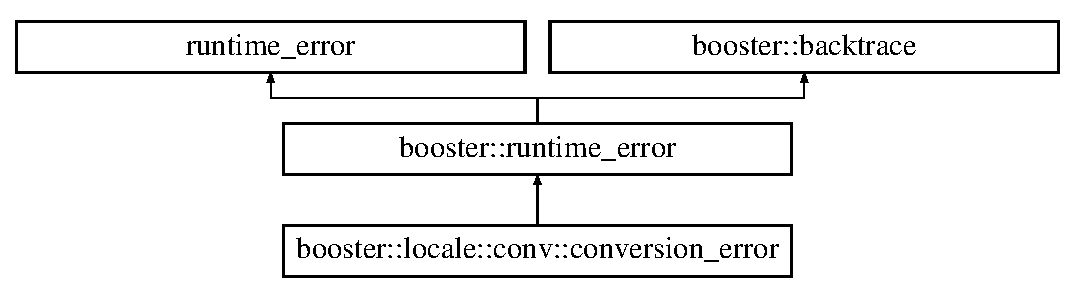
\includegraphics[height=3.000000cm]{classbooster_1_1locale_1_1conv_1_1conversion__error}
\end{center}
\end{figure}
\subsection*{Additional Inherited Members}


\subsection{Detailed Description}
The excepton that is thrown in case of conversion error. 

The documentation for this class was generated from the following file\+:\begin{DoxyCompactItemize}
\item 
booster/locale/encoding\+\_\+errors.\+h\end{DoxyCompactItemize}

\section{booster\+:\+:locale\+:\+:converter$<$ Char\+Type $>$ Class Template Reference}
\label{classbooster_1_1locale_1_1converter}\index{booster\+::locale\+::converter$<$ Char\+Type $>$@{booster\+::locale\+::converter$<$ Char\+Type $>$}}


The documentation for this class was generated from the following file\+:\begin{DoxyCompactItemize}
\item 
booster/locale/conversion.\+h\end{DoxyCompactItemize}

\section{booster\+:\+:locale\+:\+:converter$<$ char $>$ Class Template Reference}
\label{classbooster_1_1locale_1_1converter_3_01char_01_4}\index{booster\+::locale\+::converter$<$ char $>$@{booster\+::locale\+::converter$<$ char $>$}}
Inheritance diagram for booster\+:\+:locale\+:\+:converter$<$ char $>$\+:\begin{figure}[H]
\begin{center}
\leavevmode
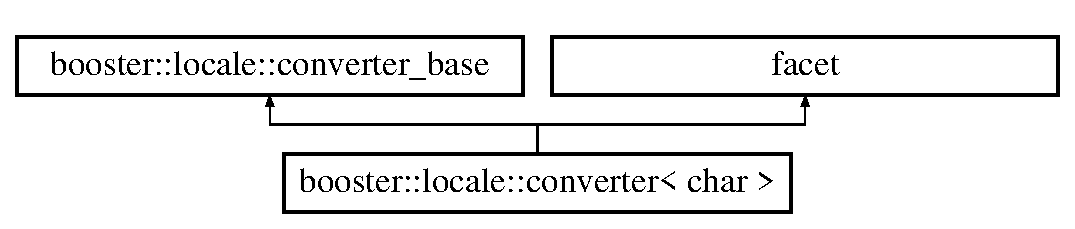
\includegraphics[height=2.000000cm]{classbooster_1_1locale_1_1converter_3_01char_01_4}
\end{center}
\end{figure}
\subsection*{Public Member Functions}
\begin{DoxyCompactItemize}
\item 
{\bfseries converter} (size\+\_\+t refs=0)\label{classbooster_1_1locale_1_1converter_3_01char_01_4_a0fe9bcea296deda0ed9217b09de2a862}

\item 
virtual std\+::string {\bfseries convert} ({\bf conversion\+\_\+type} how, char const $\ast$begin, char const $\ast$end, int flags=0) const =0\label{classbooster_1_1locale_1_1converter_3_01char_01_4_a5ef2642c11c137cb9d93368ae76b5792}

\end{DoxyCompactItemize}
\subsection*{Static Public Attributes}
\begin{DoxyCompactItemize}
\item 
static std\+::locale\+::id {\bfseries id}\label{classbooster_1_1locale_1_1converter_3_01char_01_4_a5a14a4e6600b6eae8b7ff2ea01b16a94}

\end{DoxyCompactItemize}
\subsection*{Additional Inherited Members}


The documentation for this class was generated from the following file\+:\begin{DoxyCompactItemize}
\item 
booster/locale/conversion.\+h\end{DoxyCompactItemize}

\section{booster\+:\+:locale\+:\+:converter$<$ wchar\+\_\+t $>$ Class Template Reference}
\label{classbooster_1_1locale_1_1converter_3_01wchar__t_01_4}\index{booster\+::locale\+::converter$<$ wchar\+\_\+t $>$@{booster\+::locale\+::converter$<$ wchar\+\_\+t $>$}}
Inheritance diagram for booster\+:\+:locale\+:\+:converter$<$ wchar\+\_\+t $>$\+:\begin{figure}[H]
\begin{center}
\leavevmode
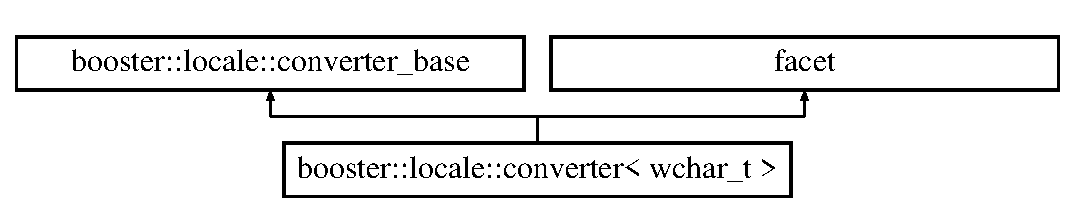
\includegraphics[height=2.000000cm]{classbooster_1_1locale_1_1converter_3_01wchar__t_01_4}
\end{center}
\end{figure}
\subsection*{Public Member Functions}
\begin{DoxyCompactItemize}
\item 
{\bfseries converter} (size\+\_\+t refs=0)\label{classbooster_1_1locale_1_1converter_3_01wchar__t_01_4_aa7adfa8dc0dd7a8482d72748da609e6a}

\item 
virtual std\+::wstring {\bfseries convert} ({\bf conversion\+\_\+type} how, wchar\+\_\+t const $\ast$begin, wchar\+\_\+t const $\ast$end, int flags=0) const =0\label{classbooster_1_1locale_1_1converter_3_01wchar__t_01_4_a692b0eda1ce3dc7254ef7eb15b95bde3}

\end{DoxyCompactItemize}
\subsection*{Static Public Attributes}
\begin{DoxyCompactItemize}
\item 
static std\+::locale\+::id {\bfseries id}\label{classbooster_1_1locale_1_1converter_3_01wchar__t_01_4_a5f9ba76a1f6e2999f3477df7d9657bf0}

\end{DoxyCompactItemize}
\subsection*{Additional Inherited Members}


The documentation for this class was generated from the following file\+:\begin{DoxyCompactItemize}
\item 
booster/locale/conversion.\+h\end{DoxyCompactItemize}

\section{booster\+:\+:locale\+:\+:converter\+\_\+base Class Reference}
\label{classbooster_1_1locale_1_1converter__base}\index{booster\+::locale\+::converter\+\_\+base@{booster\+::locale\+::converter\+\_\+base}}


This class provides base flags for text manipulation. It is used as base for converter facet.  




{\ttfamily \#include $<$booster/booster/locale/conversion.\+h$>$}

Inheritance diagram for booster\+:\+:locale\+:\+:converter\+\_\+base\+:\begin{figure}[H]
\begin{center}
\leavevmode
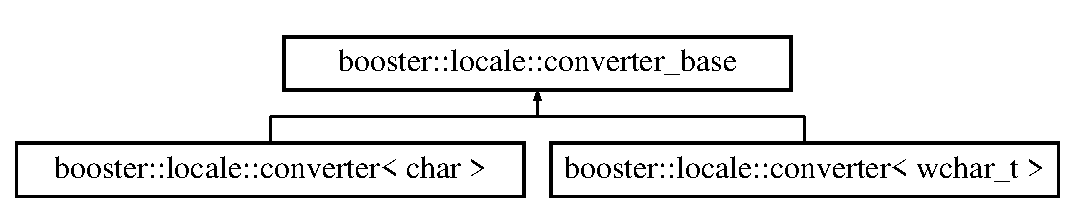
\includegraphics[height=2.000000cm]{classbooster_1_1locale_1_1converter__base}
\end{center}
\end{figure}
\subsection*{Public Types}
\begin{DoxyCompactItemize}
\item 
enum {\bf conversion\+\_\+type} \{ \\*
{\bf normalization}, 
{\bf upper\+\_\+case}, 
{\bf lower\+\_\+case}, 
{\bf case\+\_\+folding}, 
\\*
{\bf title\+\_\+case}
 \}
\end{DoxyCompactItemize}


\subsection{Detailed Description}
This class provides base flags for text manipulation. It is used as base for converter facet. 

\subsection{Member Enumeration Documentation}
\index{booster\+::locale\+::converter\+\_\+base@{booster\+::locale\+::converter\+\_\+base}!conversion\+\_\+type@{conversion\+\_\+type}}
\index{conversion\+\_\+type@{conversion\+\_\+type}!booster\+::locale\+::converter\+\_\+base@{booster\+::locale\+::converter\+\_\+base}}
\subsubsection[{conversion\+\_\+type}]{\setlength{\rightskip}{0pt plus 5cm}enum {\bf booster\+::locale\+::converter\+\_\+base\+::conversion\+\_\+type}}\label{classbooster_1_1locale_1_1converter__base_a96df87afcdd7b5cc2e2a6d67a263c3e5}
The flag used for facet -\/ the type of operation to perform \begin{Desc}
\item[Enumerator]\par
\begin{description}
\index{normalization@{normalization}!booster\+::locale\+::converter\+\_\+base@{booster\+::locale\+::converter\+\_\+base}}\index{booster\+::locale\+::converter\+\_\+base@{booster\+::locale\+::converter\+\_\+base}!normalization@{normalization}}\item[{\em 
normalization\label{classbooster_1_1locale_1_1converter__base_a96df87afcdd7b5cc2e2a6d67a263c3e5a747a6c60f9cc2b5d0517589967c966c7}
}]Apply Unicode normalization on the text. \index{upper\+\_\+case@{upper\+\_\+case}!booster\+::locale\+::converter\+\_\+base@{booster\+::locale\+::converter\+\_\+base}}\index{booster\+::locale\+::converter\+\_\+base@{booster\+::locale\+::converter\+\_\+base}!upper\+\_\+case@{upper\+\_\+case}}\item[{\em 
upper\+\_\+case\label{classbooster_1_1locale_1_1converter__base_a96df87afcdd7b5cc2e2a6d67a263c3e5af17790cf41a0295d66ad96d299baa758}
}]Convert text to upper case. \index{lower\+\_\+case@{lower\+\_\+case}!booster\+::locale\+::converter\+\_\+base@{booster\+::locale\+::converter\+\_\+base}}\index{booster\+::locale\+::converter\+\_\+base@{booster\+::locale\+::converter\+\_\+base}!lower\+\_\+case@{lower\+\_\+case}}\item[{\em 
lower\+\_\+case\label{classbooster_1_1locale_1_1converter__base_a96df87afcdd7b5cc2e2a6d67a263c3e5a857735550fa912a4529ec941a970d5ca}
}]Convert text to lower case. \index{case\+\_\+folding@{case\+\_\+folding}!booster\+::locale\+::converter\+\_\+base@{booster\+::locale\+::converter\+\_\+base}}\index{booster\+::locale\+::converter\+\_\+base@{booster\+::locale\+::converter\+\_\+base}!case\+\_\+folding@{case\+\_\+folding}}\item[{\em 
case\+\_\+folding\label{classbooster_1_1locale_1_1converter__base_a96df87afcdd7b5cc2e2a6d67a263c3e5a7cea7326b6d7426a51e5ebdedeb8fc6c}
}]Fold case in the text. \index{title\+\_\+case@{title\+\_\+case}!booster\+::locale\+::converter\+\_\+base@{booster\+::locale\+::converter\+\_\+base}}\index{booster\+::locale\+::converter\+\_\+base@{booster\+::locale\+::converter\+\_\+base}!title\+\_\+case@{title\+\_\+case}}\item[{\em 
title\+\_\+case\label{classbooster_1_1locale_1_1converter__base_a96df87afcdd7b5cc2e2a6d67a263c3e5a552f6b467b24000577867cb1009763c9}
}]Convert text to title case. \end{description}
\end{Desc}


The documentation for this class was generated from the following file\+:\begin{DoxyCompactItemize}
\item 
booster/locale/conversion.\+h\end{DoxyCompactItemize}

\section{cppcms\+:\+:http\+:\+:cookie Class Reference}
\label{classcppcms_1_1http_1_1cookie}\index{cppcms\+::http\+::cookie@{cppcms\+::http\+::cookie}}


Class that represents single H\+T\+TP Cookie Generally used in context of {\tt http\+::request} and {\tt http\+::response}.  




{\ttfamily \#include $<$cppcms/http\+\_\+cookie.\+h$>$}

\subsection*{Public Member Functions}
\begin{DoxyCompactItemize}
\item 
std\+::string {\bf name} () const 
\item 
std\+::string {\bf value} () const 
\item 
std\+::string {\bf path} () const 
\item 
std\+::string {\bf domain} () const 
\item 
std\+::string {\bf comment} () const 
\item 
bool {\bf secure} () const 
\item 
void {\bf name} (std\+::string n)
\item 
void {\bf value} (std\+::string v)
\item 
void {\bf path} (std\+::string p)
\item 
void {\bf domain} (std\+::string)
\item 
void {\bf comment} (std\+::string)
\item 
void {\bf expires} (time\+\_\+t when)
\item 
time\+\_\+t {\bf expires} () const 
\item 
bool {\bf expires\+\_\+defined} () const 
\item 
void {\bf max\+\_\+age} (unsigned age)
\item 
unsigned {\bf max\+\_\+age} () const 
\item 
bool {\bf max\+\_\+age\+\_\+defined} () const 
\item 
void {\bf browser\+\_\+age} ()
\item 
void {\bf secure} (bool v)
\item 
bool {\bf httponly} () const 
\item 
void {\bf httponly} (bool v)
\item 
bool {\bf samesite\+\_\+none} () const 
\item 
bool {\bfseries samesite\+\_\+lax} () const \label{classcppcms_1_1http_1_1cookie_a4592a2cc1ec5105f6d565a0e3d4182a4}

\item 
bool {\bfseries samesite\+\_\+strict} () const \label{classcppcms_1_1http_1_1cookie_a3a0f445903a8823f49e9acb206988232}

\item 
void {\bf samesite\+\_\+none} (bool v)
\item 
void {\bfseries samesite\+\_\+lax} (bool v)\label{classcppcms_1_1http_1_1cookie_a98f8e44a8b52237fa46bda58e7ca3fad}

\item 
void {\bfseries samesite\+\_\+strict} (bool v)\label{classcppcms_1_1http_1_1cookie_ae0036ab7b9b7d0971adc2be9e3a9bd6b}

\item 
bool {\bf empty} () const 
\item 
{\bfseries cookie} ({\bf cookie} const \&)\label{classcppcms_1_1http_1_1cookie_a499a6443b52d30660481f06242907739}

\item 
{\bfseries cookie} ({\bf cookie} \&\&)\label{classcppcms_1_1http_1_1cookie_aa150efb5be9bec3e0f1c38d6915d4cd8}

\item 
{\bf cookie} const \& {\bfseries operator=} ({\bf cookie} const \&)\label{classcppcms_1_1http_1_1cookie_a14d9c1764f457f432532e288d41265ce}

\item 
{\bf cookie} \& {\bfseries operator=} ({\bf cookie} \&\&)\label{classcppcms_1_1http_1_1cookie_a67a3aa8cb2951783c17fcbd97d261320}

\item 
{\bf cookie} (std\+::string {\bf name}, std\+::string {\bf value})
\item 
{\bf cookie} (std\+::string {\bf name}, std\+::string {\bf value}, unsigned age)
\item 
{\bf cookie} (std\+::string {\bf name}, std\+::string {\bf value}, unsigned age, std\+::string {\bf path}, std\+::string {\bf domain}=std\+::string(), std\+::string {\bf comment}=std\+::string())
\item 
{\bf cookie} (std\+::string {\bf name}, std\+::string {\bf value}, std\+::string {\bf path}, std\+::string {\bf domain}=std\+::string(), std\+::string {\bf comment}=std\+::string())\label{classcppcms_1_1http_1_1cookie_a1d0e91155e65430020350e2ab2b34a1d}

\begin{DoxyCompactList}\small\item\em Create cookie with name, value, path, domain and comment, age -\/ browser. \end{DoxyCompactList}\end{DoxyCompactItemize}
\subsection*{Friends}
\begin{DoxyCompactItemize}
\item 
std\+::ostream \& {\bfseries operator$<$$<$} (std\+::ostream \&, {\bf cookie} const \&)\label{classcppcms_1_1http_1_1cookie_a70dcba4b7aaf0804d26d88e235311b52}

\end{DoxyCompactItemize}


\subsection{Detailed Description}
Class that represents single H\+T\+TP Cookie Generally used in context of {\tt http\+::request} and {\tt http\+::response}. 

\subsection{Constructor \& Destructor Documentation}
\index{cppcms\+::http\+::cookie@{cppcms\+::http\+::cookie}!cookie@{cookie}}
\index{cookie@{cookie}!cppcms\+::http\+::cookie@{cppcms\+::http\+::cookie}}
\subsubsection[{cookie(std\+::string name, std\+::string value)}]{\setlength{\rightskip}{0pt plus 5cm}cppcms\+::http\+::cookie\+::cookie (
\begin{DoxyParamCaption}
\item[{std\+::string}]{name, }
\item[{std\+::string}]{value}
\end{DoxyParamCaption}
)}\label{classcppcms_1_1http_1_1cookie_a8acd1ff854f0c12b6b76991e8c65f39f}
Create cookie with name and value, age -\/ browser, rest properties undefined. \index{cppcms\+::http\+::cookie@{cppcms\+::http\+::cookie}!cookie@{cookie}}
\index{cookie@{cookie}!cppcms\+::http\+::cookie@{cppcms\+::http\+::cookie}}
\subsubsection[{cookie(std\+::string name, std\+::string value, unsigned age)}]{\setlength{\rightskip}{0pt plus 5cm}cppcms\+::http\+::cookie\+::cookie (
\begin{DoxyParamCaption}
\item[{std\+::string}]{name, }
\item[{std\+::string}]{value, }
\item[{unsigned}]{age}
\end{DoxyParamCaption}
)}\label{classcppcms_1_1http_1_1cookie_a9ad5a5b1cff983459b3fbbbe52c2638b}
Create cookies with name, value and max-\/age, rest properties undefined. \index{cppcms\+::http\+::cookie@{cppcms\+::http\+::cookie}!cookie@{cookie}}
\index{cookie@{cookie}!cppcms\+::http\+::cookie@{cppcms\+::http\+::cookie}}
\subsubsection[{cookie(std\+::string name, std\+::string value, unsigned age, std\+::string path, std\+::string domain=std\+::string(), std\+::string comment=std\+::string())}]{\setlength{\rightskip}{0pt plus 5cm}cppcms\+::http\+::cookie\+::cookie (
\begin{DoxyParamCaption}
\item[{std\+::string}]{name, }
\item[{std\+::string}]{value, }
\item[{unsigned}]{age, }
\item[{std\+::string}]{path, }
\item[{std\+::string}]{domain = {\ttfamily std\+:\+:string()}, }
\item[{std\+::string}]{comment = {\ttfamily std\+:\+:string()}}
\end{DoxyParamCaption}
)}\label{classcppcms_1_1http_1_1cookie_a0f0f0843f124d11cda1dd3a6ab194c2a}
Create cookie with name, value, max-\/age, path, domain and command 

\subsection{Member Function Documentation}
\index{cppcms\+::http\+::cookie@{cppcms\+::http\+::cookie}!browser\+\_\+age@{browser\+\_\+age}}
\index{browser\+\_\+age@{browser\+\_\+age}!cppcms\+::http\+::cookie@{cppcms\+::http\+::cookie}}
\subsubsection[{browser\+\_\+age()}]{\setlength{\rightskip}{0pt plus 5cm}void cppcms\+::http\+::cookie\+::browser\+\_\+age (
\begin{DoxyParamCaption}
{}
\end{DoxyParamCaption}
)}\label{classcppcms_1_1http_1_1cookie_ae711598846c4cf198100d18e81387fd7}
Set age according to browser\textquotesingle{}s session (i.\+e. no Max-\/\+Age) \index{cppcms\+::http\+::cookie@{cppcms\+::http\+::cookie}!comment@{comment}}
\index{comment@{comment}!cppcms\+::http\+::cookie@{cppcms\+::http\+::cookie}}
\subsubsection[{comment() const }]{\setlength{\rightskip}{0pt plus 5cm}std\+::string cppcms\+::http\+::cookie\+::comment (
\begin{DoxyParamCaption}
{}
\end{DoxyParamCaption}
) const}\label{classcppcms_1_1http_1_1cookie_a3d65d0792f011e30a31c0ad1d65cab73}
Cookie\textquotesingle{}s comment \index{cppcms\+::http\+::cookie@{cppcms\+::http\+::cookie}!comment@{comment}}
\index{comment@{comment}!cppcms\+::http\+::cookie@{cppcms\+::http\+::cookie}}
\subsubsection[{comment(std\+::string)}]{\setlength{\rightskip}{0pt plus 5cm}void cppcms\+::http\+::cookie\+::comment (
\begin{DoxyParamCaption}
\item[{std\+::string}]{}
\end{DoxyParamCaption}
)}\label{classcppcms_1_1http_1_1cookie_abf5ffd21c8f28e9b1f6b60e7de78fe81}
Set cookie\textquotesingle{}s comment \index{cppcms\+::http\+::cookie@{cppcms\+::http\+::cookie}!domain@{domain}}
\index{domain@{domain}!cppcms\+::http\+::cookie@{cppcms\+::http\+::cookie}}
\subsubsection[{domain() const }]{\setlength{\rightskip}{0pt plus 5cm}std\+::string cppcms\+::http\+::cookie\+::domain (
\begin{DoxyParamCaption}
{}
\end{DoxyParamCaption}
) const}\label{classcppcms_1_1http_1_1cookie_a4f1f52f877462585bfbd65a72d510c5d}
Cookie\textquotesingle{}s domain \index{cppcms\+::http\+::cookie@{cppcms\+::http\+::cookie}!domain@{domain}}
\index{domain@{domain}!cppcms\+::http\+::cookie@{cppcms\+::http\+::cookie}}
\subsubsection[{domain(std\+::string)}]{\setlength{\rightskip}{0pt plus 5cm}void cppcms\+::http\+::cookie\+::domain (
\begin{DoxyParamCaption}
\item[{std\+::string}]{}
\end{DoxyParamCaption}
)}\label{classcppcms_1_1http_1_1cookie_a77913118efb2bec104e7af3e999c3fc3}
Set cookie\textquotesingle{}s domain \index{cppcms\+::http\+::cookie@{cppcms\+::http\+::cookie}!empty@{empty}}
\index{empty@{empty}!cppcms\+::http\+::cookie@{cppcms\+::http\+::cookie}}
\subsubsection[{empty() const }]{\setlength{\rightskip}{0pt plus 5cm}bool cppcms\+::http\+::cookie\+::empty (
\begin{DoxyParamCaption}
{}
\end{DoxyParamCaption}
) const}\label{classcppcms_1_1http_1_1cookie_ac295303fc67b91e04ed050c8ad2ef539}
Check if cookie is not assigned -\/ empty \index{cppcms\+::http\+::cookie@{cppcms\+::http\+::cookie}!expires@{expires}}
\index{expires@{expires}!cppcms\+::http\+::cookie@{cppcms\+::http\+::cookie}}
\subsubsection[{expires(time\+\_\+t when)}]{\setlength{\rightskip}{0pt plus 5cm}void cppcms\+::http\+::cookie\+::expires (
\begin{DoxyParamCaption}
\item[{time\+\_\+t}]{when}
\end{DoxyParamCaption}
)}\label{classcppcms_1_1http_1_1cookie_a4db7c3df34aed3db80424bfd7d7b40f0}
Set expiration date/time \index{cppcms\+::http\+::cookie@{cppcms\+::http\+::cookie}!expires@{expires}}
\index{expires@{expires}!cppcms\+::http\+::cookie@{cppcms\+::http\+::cookie}}
\subsubsection[{expires() const }]{\setlength{\rightskip}{0pt plus 5cm}time\+\_\+t cppcms\+::http\+::cookie\+::expires (
\begin{DoxyParamCaption}
{}
\end{DoxyParamCaption}
) const}\label{classcppcms_1_1http_1_1cookie_aa3b93d74bd89e16dc4632bb8fee6c442}
Returns expires timestamp for the cookie, if not set returns 0

\doxyref{New in Cpp\+C\+MS 1.\+2}{p.}{v1_2} \index{cppcms\+::http\+::cookie@{cppcms\+::http\+::cookie}!expires\+\_\+defined@{expires\+\_\+defined}}
\index{expires\+\_\+defined@{expires\+\_\+defined}!cppcms\+::http\+::cookie@{cppcms\+::http\+::cookie}}
\subsubsection[{expires\+\_\+defined() const }]{\setlength{\rightskip}{0pt plus 5cm}bool cppcms\+::http\+::cookie\+::expires\+\_\+defined (
\begin{DoxyParamCaption}
{}
\end{DoxyParamCaption}
) const}\label{classcppcms_1_1http_1_1cookie_a74d49f2e5c1180e1a62bb7867eed50ee}
returns true if \doxyref{expires(time\+\_\+t when)}{p.}{classcppcms_1_1http_1_1cookie_a4db7c3df34aed3db80424bfd7d7b40f0} was called and expiration was set, if \doxyref{browser\+\_\+age()}{p.}{classcppcms_1_1http_1_1cookie_ae711598846c4cf198100d18e81387fd7} is called it is reset to false

\doxyref{New in Cpp\+C\+MS 1.\+2}{p.}{v1_2} \index{cppcms\+::http\+::cookie@{cppcms\+::http\+::cookie}!httponly@{httponly}}
\index{httponly@{httponly}!cppcms\+::http\+::cookie@{cppcms\+::http\+::cookie}}
\subsubsection[{httponly() const }]{\setlength{\rightskip}{0pt plus 5cm}bool cppcms\+::http\+::cookie\+::httponly (
\begin{DoxyParamCaption}
{}
\end{DoxyParamCaption}
) const}\label{classcppcms_1_1http_1_1cookie_ad7a7e284d7e50f2e5ff6458048fdf172}
Check if the httponly propertie is set on the cookies \index{cppcms\+::http\+::cookie@{cppcms\+::http\+::cookie}!httponly@{httponly}}
\index{httponly@{httponly}!cppcms\+::http\+::cookie@{cppcms\+::http\+::cookie}}
\subsubsection[{httponly(bool v)}]{\setlength{\rightskip}{0pt plus 5cm}void cppcms\+::http\+::cookie\+::httponly (
\begin{DoxyParamCaption}
\item[{bool}]{v}
\end{DoxyParamCaption}
)}\label{classcppcms_1_1http_1_1cookie_a7a2f9bddbf36750023e20cab47f08d3a}
Set httponly property on the cookies \index{cppcms\+::http\+::cookie@{cppcms\+::http\+::cookie}!max\+\_\+age@{max\+\_\+age}}
\index{max\+\_\+age@{max\+\_\+age}!cppcms\+::http\+::cookie@{cppcms\+::http\+::cookie}}
\subsubsection[{max\+\_\+age(unsigned age)}]{\setlength{\rightskip}{0pt plus 5cm}void cppcms\+::http\+::cookie\+::max\+\_\+age (
\begin{DoxyParamCaption}
\item[{unsigned}]{age}
\end{DoxyParamCaption}
)}\label{classcppcms_1_1http_1_1cookie_a477b841aa9dee6894a5989153ee16df0}
Set max cookie\textquotesingle{}s age \index{cppcms\+::http\+::cookie@{cppcms\+::http\+::cookie}!max\+\_\+age@{max\+\_\+age}}
\index{max\+\_\+age@{max\+\_\+age}!cppcms\+::http\+::cookie@{cppcms\+::http\+::cookie}}
\subsubsection[{max\+\_\+age() const }]{\setlength{\rightskip}{0pt plus 5cm}unsigned cppcms\+::http\+::cookie\+::max\+\_\+age (
\begin{DoxyParamCaption}
{}
\end{DoxyParamCaption}
) const}\label{classcppcms_1_1http_1_1cookie_a295822f3cc0798ff5f3821d723ef8542}
Get max cookie\textquotesingle{}s age, returns 0 if not set

\doxyref{New in Cpp\+C\+MS 1.\+2}{p.}{v1_2} \index{cppcms\+::http\+::cookie@{cppcms\+::http\+::cookie}!max\+\_\+age\+\_\+defined@{max\+\_\+age\+\_\+defined}}
\index{max\+\_\+age\+\_\+defined@{max\+\_\+age\+\_\+defined}!cppcms\+::http\+::cookie@{cppcms\+::http\+::cookie}}
\subsubsection[{max\+\_\+age\+\_\+defined() const }]{\setlength{\rightskip}{0pt plus 5cm}bool cppcms\+::http\+::cookie\+::max\+\_\+age\+\_\+defined (
\begin{DoxyParamCaption}
{}
\end{DoxyParamCaption}
) const}\label{classcppcms_1_1http_1_1cookie_a39955f1b8b4e87ca88cc6698c2b3dbd8}
returns true if max(unsigned age) was called and max\+\_\+age was set, if \doxyref{browser\+\_\+age()}{p.}{classcppcms_1_1http_1_1cookie_ae711598846c4cf198100d18e81387fd7} is called it is reset to false

\doxyref{New in Cpp\+C\+MS 1.\+2}{p.}{v1_2} \index{cppcms\+::http\+::cookie@{cppcms\+::http\+::cookie}!name@{name}}
\index{name@{name}!cppcms\+::http\+::cookie@{cppcms\+::http\+::cookie}}
\subsubsection[{name() const }]{\setlength{\rightskip}{0pt plus 5cm}std\+::string cppcms\+::http\+::cookie\+::name (
\begin{DoxyParamCaption}
{}
\end{DoxyParamCaption}
) const}\label{classcppcms_1_1http_1_1cookie_a73670fe5dbf1b69907478748dc4ccf47}
Cookie\textquotesingle{}s Name \index{cppcms\+::http\+::cookie@{cppcms\+::http\+::cookie}!name@{name}}
\index{name@{name}!cppcms\+::http\+::cookie@{cppcms\+::http\+::cookie}}
\subsubsection[{name(std\+::string n)}]{\setlength{\rightskip}{0pt plus 5cm}void cppcms\+::http\+::cookie\+::name (
\begin{DoxyParamCaption}
\item[{std\+::string}]{n}
\end{DoxyParamCaption}
)}\label{classcppcms_1_1http_1_1cookie_a5254844ef302d1b4ea2f6e031d27a994}
Set cookie\textquotesingle{}s name \index{cppcms\+::http\+::cookie@{cppcms\+::http\+::cookie}!path@{path}}
\index{path@{path}!cppcms\+::http\+::cookie@{cppcms\+::http\+::cookie}}
\subsubsection[{path() const }]{\setlength{\rightskip}{0pt plus 5cm}std\+::string cppcms\+::http\+::cookie\+::path (
\begin{DoxyParamCaption}
{}
\end{DoxyParamCaption}
) const}\label{classcppcms_1_1http_1_1cookie_a3b5aa9f22d923fe230e747cbb8b41db0}
Cookie\textquotesingle{}s path \index{cppcms\+::http\+::cookie@{cppcms\+::http\+::cookie}!path@{path}}
\index{path@{path}!cppcms\+::http\+::cookie@{cppcms\+::http\+::cookie}}
\subsubsection[{path(std\+::string p)}]{\setlength{\rightskip}{0pt plus 5cm}void cppcms\+::http\+::cookie\+::path (
\begin{DoxyParamCaption}
\item[{std\+::string}]{p}
\end{DoxyParamCaption}
)}\label{classcppcms_1_1http_1_1cookie_a3afa090f85bff64bdd5085b6b48482c7}
Set cookie\textquotesingle{}s path \index{cppcms\+::http\+::cookie@{cppcms\+::http\+::cookie}!samesite\+\_\+none@{samesite\+\_\+none}}
\index{samesite\+\_\+none@{samesite\+\_\+none}!cppcms\+::http\+::cookie@{cppcms\+::http\+::cookie}}
\subsubsection[{samesite\+\_\+none() const }]{\setlength{\rightskip}{0pt plus 5cm}bool cppcms\+::http\+::cookie\+::samesite\+\_\+none (
\begin{DoxyParamCaption}
{}
\end{DoxyParamCaption}
) const}\label{classcppcms_1_1http_1_1cookie_ac2ecd673811caf6c83c40a4f2c5b4885}
Check if one of the samesite properties is set on the cookies \index{cppcms\+::http\+::cookie@{cppcms\+::http\+::cookie}!samesite\+\_\+none@{samesite\+\_\+none}}
\index{samesite\+\_\+none@{samesite\+\_\+none}!cppcms\+::http\+::cookie@{cppcms\+::http\+::cookie}}
\subsubsection[{samesite\+\_\+none(bool v)}]{\setlength{\rightskip}{0pt plus 5cm}void cppcms\+::http\+::cookie\+::samesite\+\_\+none (
\begin{DoxyParamCaption}
\item[{bool}]{v}
\end{DoxyParamCaption}
)}\label{classcppcms_1_1http_1_1cookie_a9a8fc5889a3e55b7d178db046cd809af}
Set one of the samesite properties on the cookies \index{cppcms\+::http\+::cookie@{cppcms\+::http\+::cookie}!secure@{secure}}
\index{secure@{secure}!cppcms\+::http\+::cookie@{cppcms\+::http\+::cookie}}
\subsubsection[{secure() const }]{\setlength{\rightskip}{0pt plus 5cm}bool cppcms\+::http\+::cookie\+::secure (
\begin{DoxyParamCaption}
{}
\end{DoxyParamCaption}
) const}\label{classcppcms_1_1http_1_1cookie_a819a66699f59e2c90165bdcba57107d1}
Check if the cookie is transferred over secure connection only \index{cppcms\+::http\+::cookie@{cppcms\+::http\+::cookie}!secure@{secure}}
\index{secure@{secure}!cppcms\+::http\+::cookie@{cppcms\+::http\+::cookie}}
\subsubsection[{secure(bool v)}]{\setlength{\rightskip}{0pt plus 5cm}void cppcms\+::http\+::cookie\+::secure (
\begin{DoxyParamCaption}
\item[{bool}]{v}
\end{DoxyParamCaption}
)}\label{classcppcms_1_1http_1_1cookie_a4b905fc3fdaa374a72bb52d6d892d176}
Set secure property on the cookies \index{cppcms\+::http\+::cookie@{cppcms\+::http\+::cookie}!value@{value}}
\index{value@{value}!cppcms\+::http\+::cookie@{cppcms\+::http\+::cookie}}
\subsubsection[{value() const }]{\setlength{\rightskip}{0pt plus 5cm}std\+::string cppcms\+::http\+::cookie\+::value (
\begin{DoxyParamCaption}
{}
\end{DoxyParamCaption}
) const}\label{classcppcms_1_1http_1_1cookie_a5f62fe58389118843d35b474a2c2fed3}
Cookie\textquotesingle{}s value \index{cppcms\+::http\+::cookie@{cppcms\+::http\+::cookie}!value@{value}}
\index{value@{value}!cppcms\+::http\+::cookie@{cppcms\+::http\+::cookie}}
\subsubsection[{value(std\+::string v)}]{\setlength{\rightskip}{0pt plus 5cm}void cppcms\+::http\+::cookie\+::value (
\begin{DoxyParamCaption}
\item[{std\+::string}]{v}
\end{DoxyParamCaption}
)}\label{classcppcms_1_1http_1_1cookie_ae85d53dccffa7b940131d4b09f47241e}
Set cookie\textquotesingle{}s value 

The documentation for this class was generated from the following file\+:\begin{DoxyCompactItemize}
\item 
cppcms/http\+\_\+cookie.\+h\end{DoxyCompactItemize}

\section{cppcms\+:\+:copy\+\_\+filter Class Reference}
\label{classcppcms_1_1copy__filter}\index{cppcms\+::copy\+\_\+filter@{cppcms\+::copy\+\_\+filter}}


Copy the output stream part -\/ \char`\"{}tee\char`\"{} filter.  




{\ttfamily \#include $<$cppcms/copy\+\_\+filter.\+h$>$}

Inheritance diagram for cppcms\+:\+:copy\+\_\+filter\+:\begin{figure}[H]
\begin{center}
\leavevmode
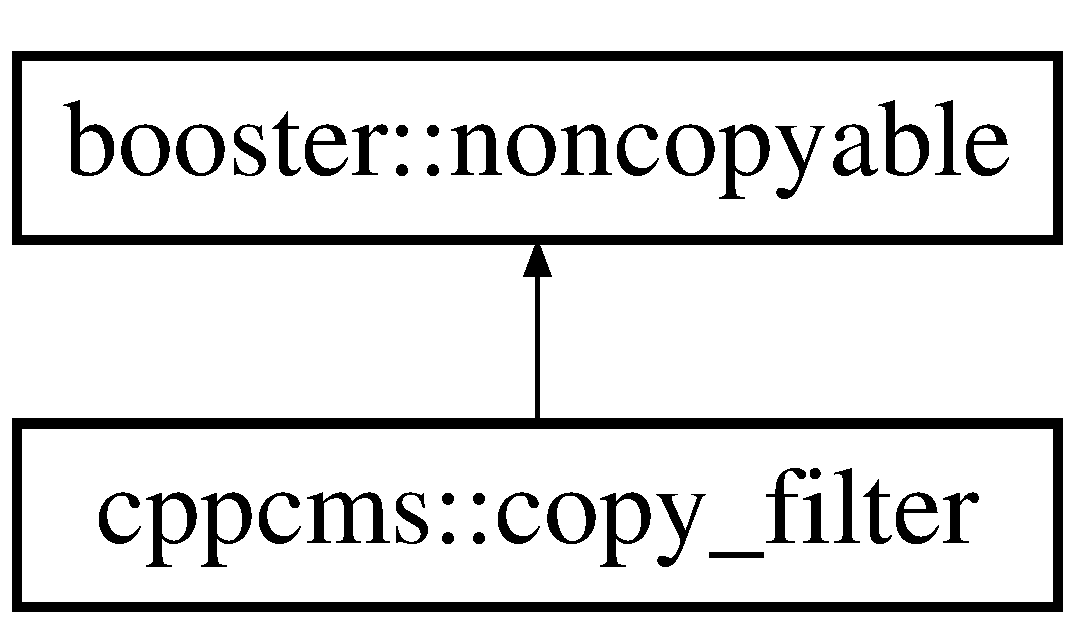
\includegraphics[height=2.000000cm]{classcppcms_1_1copy__filter}
\end{center}
\end{figure}
\subsection*{Public Member Functions}
\begin{DoxyCompactItemize}
\item 
{\bf copy\+\_\+filter} (std\+::ostream \&output)
\item 
{\bf $\sim$copy\+\_\+filter} ()
\item 
std\+::string {\bf detach} ()
\end{DoxyCompactItemize}


\subsection{Detailed Description}
Copy the output stream part -\/ \char`\"{}tee\char`\"{} filter. 

This simple class designed to \char`\"{}copy\char`\"{} all the output that comes to the stream to internal buffer and the stream itself and return the copied data on detaching the filter.

It is very useful to use with caching, for example\+:


\begin{DoxyCode}
std::string frame;
\textcolor{keywordflow}{if}(cache().fetch\_frame(\textcolor{stringliteral}{"key"},frame)) \{
  out() << frame;
\}
\textcolor{keywordflow}{else} \{
  cppcms::copy_filter tee(out());
  ...
  \textcolor{comment}{// generate something heavy}
  ...
  cache().store\_frame(\textcolor{stringliteral}{"key"},tee.detach());
\}
\end{DoxyCode}
 

\subsection{Constructor \& Destructor Documentation}
\index{cppcms\+::copy\+\_\+filter@{cppcms\+::copy\+\_\+filter}!copy\+\_\+filter@{copy\+\_\+filter}}
\index{copy\+\_\+filter@{copy\+\_\+filter}!cppcms\+::copy\+\_\+filter@{cppcms\+::copy\+\_\+filter}}
\subsubsection[{copy\+\_\+filter(std\+::ostream \&output)}]{\setlength{\rightskip}{0pt plus 5cm}cppcms\+::copy\+\_\+filter\+::copy\+\_\+filter (
\begin{DoxyParamCaption}
\item[{std\+::ostream \&}]{output}
\end{DoxyParamCaption}
)}\label{classcppcms_1_1copy__filter_a5af43360706ba459dcdfb2bb89b01b7e}
Create a filter copying all output to internal buffer \index{cppcms\+::copy\+\_\+filter@{cppcms\+::copy\+\_\+filter}!````~copy\+\_\+filter@{$\sim$copy\+\_\+filter}}
\index{````~copy\+\_\+filter@{$\sim$copy\+\_\+filter}!cppcms\+::copy\+\_\+filter@{cppcms\+::copy\+\_\+filter}}
\subsubsection[{$\sim$copy\+\_\+filter()}]{\setlength{\rightskip}{0pt plus 5cm}cppcms\+::copy\+\_\+filter\+::$\sim$copy\+\_\+filter (
\begin{DoxyParamCaption}
{}
\end{DoxyParamCaption}
)}\label{classcppcms_1_1copy__filter_a9c72ba16b11ffb485f4c6ff79397e608}
When destroyed, if the stream wasn\textquotesingle{}t detached aborts coping the data, making it exception safe. 

\subsection{Member Function Documentation}
\index{cppcms\+::copy\+\_\+filter@{cppcms\+::copy\+\_\+filter}!detach@{detach}}
\index{detach@{detach}!cppcms\+::copy\+\_\+filter@{cppcms\+::copy\+\_\+filter}}
\subsubsection[{detach()}]{\setlength{\rightskip}{0pt plus 5cm}std\+::string cppcms\+::copy\+\_\+filter\+::detach (
\begin{DoxyParamCaption}
{}
\end{DoxyParamCaption}
)}\label{classcppcms_1_1copy__filter_a39db5af5ab6f59edbc15f3324c7950df}
Stop the coping process and return all collected data as string. 

The documentation for this class was generated from the following file\+:\begin{DoxyCompactItemize}
\item 
cppcms/copy\+\_\+filter.\+h\end{DoxyCompactItemize}

\section{booster\+:\+:copy\+\_\+ptr$<$ T $>$ Class Template Reference}
\label{classbooster_1_1copy__ptr}\index{booster\+::copy\+\_\+ptr$<$ T $>$@{booster\+::copy\+\_\+ptr$<$ T $>$}}


a smart pointer similar to std\+::unique\+\_\+ptr but it copies underlying object on pointer copy instead of moving its ownership.  




{\ttfamily \#include $<$booster/booster/copy\+\_\+ptr.\+h$>$}

\subsection*{Public Member Functions}
\begin{DoxyCompactItemize}
\item 
{\bfseries copy\+\_\+ptr} (T $\ast$v)\label{classbooster_1_1copy__ptr_accc428d4c2e0bbc215dcdfaa19e76dc6}

\item 
{\bfseries copy\+\_\+ptr} ({\bf copy\+\_\+ptr} const \&other)\label{classbooster_1_1copy__ptr_a8990363c8a2ea8b66d34a3099fae9bd4}

\item 
{\bfseries copy\+\_\+ptr} ({\bf copy\+\_\+ptr} \&\&other)\label{classbooster_1_1copy__ptr_a7afe98b7b9038af1f1a7e51c1894d847}

\item 
{\bf copy\+\_\+ptr} \& {\bfseries operator=} ({\bf copy\+\_\+ptr} \&\&other)\label{classbooster_1_1copy__ptr_a6de572b8aff0b4647a91e742a7bc2e1b}

\item 
{\bf copy\+\_\+ptr} const \& {\bfseries operator=} ({\bf copy\+\_\+ptr} const \&other)\label{classbooster_1_1copy__ptr_a692c395662fd08916ca79b3e5cc01df9}

\item 
T const $\ast$ {\bfseries get} () const \label{classbooster_1_1copy__ptr_ab2bafeae3949e6d137fc75f4dc47c154}

\item 
T $\ast$ {\bfseries get} ()\label{classbooster_1_1copy__ptr_a691964944093292970331a92bed64848}

\item 
T const \& {\bfseries operator$\ast$} () const \label{classbooster_1_1copy__ptr_a759a3effd74fd7d77e4a291fca62f99b}

\item 
T \& {\bfseries operator$\ast$} ()\label{classbooster_1_1copy__ptr_ab62472e58eab77c44ba703e96a5cf6bc}

\item 
T const $\ast$ {\bfseries operator-\/$>$} () const \label{classbooster_1_1copy__ptr_a47548c62ecc194e384ab8dd21bd4c1ff}

\item 
T $\ast$ {\bfseries operator-\/$>$} ()\label{classbooster_1_1copy__ptr_aa12d0c6e0e12a4354256d15b82daeb9e}

\item 
T $\ast$ {\bfseries release} ()\label{classbooster_1_1copy__ptr_a4b9ebbe86e33e45bcd9aa0f47d57c9cd}

\item 
void {\bfseries reset} (T $\ast$p=0)\label{classbooster_1_1copy__ptr_a94831913ae1253ba483c9356a440c71b}

\item 
void {\bfseries swap} ({\bf copy\+\_\+ptr} \&other)\label{classbooster_1_1copy__ptr_a3ae4ac0b6041dd1cd226d76333333e00}

\end{DoxyCompactItemize}


\subsection{Detailed Description}
\subsubsection*{template$<$typename T$>$\\*
class booster\+::copy\+\_\+ptr$<$ T $>$}

a smart pointer similar to std\+::unique\+\_\+ptr but it copies underlying object on pointer copy instead of moving its ownership. 

Note\+: Underlying object has same constness as the pointer itself (not like in ordinary pointer).

Don\textquotesingle{}t use it with polymorphic classes. Prefer \doxyref{clone\+\_\+ptr}{p.}{classbooster_1_1clone__ptr} instead. 

The documentation for this class was generated from the following file\+:\begin{DoxyCompactItemize}
\item 
booster/copy\+\_\+ptr.\+h\end{DoxyCompactItemize}

\section{cppcms\+:\+:cppcms\+\_\+error Class Reference}
\label{classcppcms_1_1cppcms__error}\index{cppcms\+::cppcms\+\_\+error@{cppcms\+::cppcms\+\_\+error}}


Exception thrown by Cpp\+C\+MS framework.  




{\ttfamily \#include $<$cppcms/cppcms\+\_\+error.\+h$>$}

Inheritance diagram for cppcms\+:\+:cppcms\+\_\+error\+:\begin{figure}[H]
\begin{center}
\leavevmode
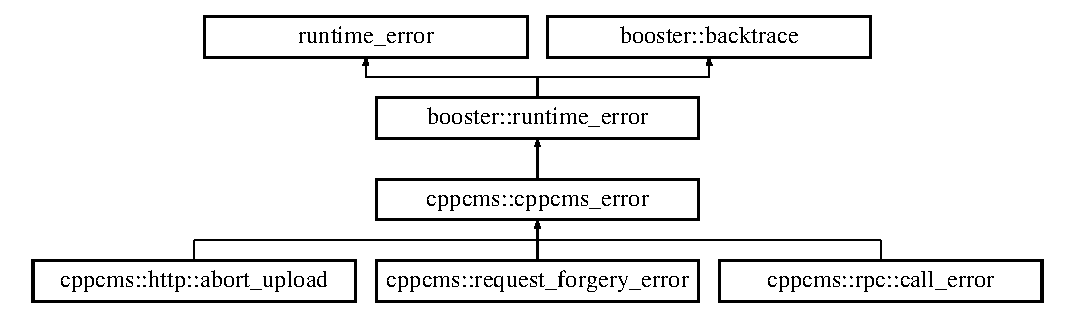
\includegraphics[height=3.829060cm]{classcppcms_1_1cppcms__error}
\end{center}
\end{figure}
\subsection*{Public Member Functions}
\begin{DoxyCompactItemize}
\item 
{\bf cppcms\+\_\+error} (int err, std\+::string const \&error)
\item 
{\bf cppcms\+\_\+error} (std\+::string const \&error)
\end{DoxyCompactItemize}
\subsection*{Additional Inherited Members}


\subsection{Detailed Description}
Exception thrown by Cpp\+C\+MS framework. 

Every exception that is thrown from Cpp\+C\+MS modules derived from this exception. 

\subsection{Constructor \& Destructor Documentation}
\index{cppcms\+::cppcms\+\_\+error@{cppcms\+::cppcms\+\_\+error}!cppcms\+\_\+error@{cppcms\+\_\+error}}
\index{cppcms\+\_\+error@{cppcms\+\_\+error}!cppcms\+::cppcms\+\_\+error@{cppcms\+::cppcms\+\_\+error}}
\subsubsection[{cppcms\+\_\+error(int err, std\+::string const \&error)}]{\setlength{\rightskip}{0pt plus 5cm}cppcms\+::cppcms\+\_\+error\+::cppcms\+\_\+error (
\begin{DoxyParamCaption}
\item[{int}]{err, }
\item[{std\+::string const \&}]{error}
\end{DoxyParamCaption}
)}\label{classcppcms_1_1cppcms__error_a8b3d19ee492b926c96adb625436c0347}
Create an object with error code err (errno) and a message {\itshape error} \index{cppcms\+::cppcms\+\_\+error@{cppcms\+::cppcms\+\_\+error}!cppcms\+\_\+error@{cppcms\+\_\+error}}
\index{cppcms\+\_\+error@{cppcms\+\_\+error}!cppcms\+::cppcms\+\_\+error@{cppcms\+::cppcms\+\_\+error}}
\subsubsection[{cppcms\+\_\+error(std\+::string const \&error)}]{\setlength{\rightskip}{0pt plus 5cm}cppcms\+::cppcms\+\_\+error\+::cppcms\+\_\+error (
\begin{DoxyParamCaption}
\item[{std\+::string const \&}]{error}
\end{DoxyParamCaption}
)\hspace{0.3cm}{\ttfamily [inline]}}\label{classcppcms_1_1cppcms__error_adf4667d22acccb0c2f8c78a003b7de7c}
Create an object with message {\itshape error} 

The documentation for this class was generated from the following file\+:\begin{DoxyCompactItemize}
\item 
cppcms/cppcms\+\_\+error.\+h\end{DoxyCompactItemize}

\section{cppcms\+:\+:filters\+:\+:date Class Reference}
\label{classcppcms_1_1filters_1_1date}\index{cppcms\+::filters\+::date@{cppcms\+::filters\+::date}}


Formats date to the stream, date is represented as number -\/ P\+O\+S\+IX time, a plain number.  




{\ttfamily \#include $<$cppcms/filters.\+h$>$}

\subsection*{Public Member Functions}
\begin{DoxyCompactItemize}
\item 
{\bfseries date} ({\bf date} const \&other)\label{classcppcms_1_1filters_1_1date_ab53643381fd5cc58c4350747ac86f049}

\item 
{\bf date} const \& {\bfseries operator=} ({\bf date} const \&other)\label{classcppcms_1_1filters_1_1date_a4530a894d551d081f0f480d6de2087b5}

\item 
{\bf date} ({\bf streamable} const \&{\bf time})
\item 
{\bf date} ({\bf streamable} const \&{\bf time}, std\+::string const \&timezone)
\item 
void {\bfseries operator()} (std\+::ostream \&out) const \label{classcppcms_1_1filters_1_1date_aba324cd826342dcec5f64d12ebb846a1}

\end{DoxyCompactItemize}


\subsection{Detailed Description}
Formats date to the stream, date is represented as number -\/ P\+O\+S\+IX time, a plain number. 

\subsection{Constructor \& Destructor Documentation}
\index{cppcms\+::filters\+::date@{cppcms\+::filters\+::date}!date@{date}}
\index{date@{date}!cppcms\+::filters\+::date@{cppcms\+::filters\+::date}}
\subsubsection[{date(streamable const \&time)}]{\setlength{\rightskip}{0pt plus 5cm}cppcms\+::filters\+::date\+::date (
\begin{DoxyParamCaption}
\item[{{\bf streamable} const \&}]{time}
\end{DoxyParamCaption}
)}\label{classcppcms_1_1filters_1_1date_a0f3c8e723f9500a635901705bad074fc}
Create date filter that formats current local-\/time date using P\+O\+S\+IX time representation {\itshape time} \index{cppcms\+::filters\+::date@{cppcms\+::filters\+::date}!date@{date}}
\index{date@{date}!cppcms\+::filters\+::date@{cppcms\+::filters\+::date}}
\subsubsection[{date(streamable const \&time, std\+::string const \&timezone)}]{\setlength{\rightskip}{0pt plus 5cm}cppcms\+::filters\+::date\+::date (
\begin{DoxyParamCaption}
\item[{{\bf streamable} const \&}]{time, }
\item[{std\+::string const \&}]{timezone}
\end{DoxyParamCaption}
)}\label{classcppcms_1_1filters_1_1date_afada03ed77f7c09f36043b9d6ff8fd28}
Create date filter that formats current date using P\+O\+S\+IX time representation {\itshape time}, in a timezone {\itshape timezone} 

The documentation for this class was generated from the following file\+:\begin{DoxyCompactItemize}
\item 
cppcms/filters.\+h\end{DoxyCompactItemize}

\section{booster\+:\+:locale\+:\+:date\+\_\+time Class Reference}
\label{classbooster_1_1locale_1_1date__time}\index{booster\+::locale\+::date\+\_\+time@{booster\+::locale\+::date\+\_\+time}}


this class represents a date time and allows to perform various operation according to the locale settings.  




{\ttfamily \#include $<$booster/booster/locale/date\+\_\+time.\+h$>$}

\subsection*{Public Member Functions}
\begin{DoxyCompactItemize}
\item 
{\bf date\+\_\+time} ()
\item 
{\bf date\+\_\+time} ({\bf date\+\_\+time} const \&other)
\item 
{\bf date\+\_\+time} ({\bf date\+\_\+time} const \&other, {\bf date\+\_\+time\+\_\+period\+\_\+set} const \&{\bf set})
\item 
{\bf date\+\_\+time} const \& {\bf operator=} ({\bf date\+\_\+time} const \&other)
\item 
{\bf date\+\_\+time} (double {\bf time})
\item 
{\bf date\+\_\+time} (double {\bf time}, {\bf calendar} const \&cal)
\item 
{\bf date\+\_\+time} ({\bf calendar} const \&cal)
\item 
{\bf date\+\_\+time} ({\bf date\+\_\+time\+\_\+period\+\_\+set} const \&{\bf set})
\item 
{\bf date\+\_\+time} ({\bf date\+\_\+time\+\_\+period\+\_\+set} const \&{\bf set}, {\bf calendar} const \&cal)
\item 
{\bf date\+\_\+time} const \& {\bf operator=} ({\bf date\+\_\+time\+\_\+period\+\_\+set} const \&f)
\item 
void {\bf set} ({\bf period\+::period\+\_\+type} f, int v)
\item 
int {\bf get} ({\bf period\+::period\+\_\+type} f) const 
\item 
int {\bf operator/} ({\bf period\+::period\+\_\+type} f) const 
\item 
{\bf date\+\_\+time} {\bf operator+} ({\bf period\+::period\+\_\+type} f) const 
\item 
{\bf date\+\_\+time} {\bf operator-\/} ({\bf period\+::period\+\_\+type} f) const 
\item 
{\bf date\+\_\+time} const \& {\bf operator+=} ({\bf period\+::period\+\_\+type} f)
\item 
{\bf date\+\_\+time} const \& {\bf operator-\/=} ({\bf period\+::period\+\_\+type} f)
\item 
{\bf date\+\_\+time} {\bf operator$<$$<$} ({\bf period\+::period\+\_\+type} f) const 
\item 
{\bf date\+\_\+time} {\bf operator$>$$>$} ({\bf period\+::period\+\_\+type} f) const 
\item 
{\bf date\+\_\+time} const \& {\bf operator$<$$<$=} ({\bf period\+::period\+\_\+type} f)
\item 
{\bf date\+\_\+time} const \& {\bf operator$>$$>$=} ({\bf period\+::period\+\_\+type} f)
\item 
{\bf date\+\_\+time} {\bf operator+} ({\bf date\+\_\+time\+\_\+period} const \&v) const 
\item 
{\bf date\+\_\+time} {\bf operator-\/} ({\bf date\+\_\+time\+\_\+period} const \&v) const 
\item 
{\bf date\+\_\+time} const \& {\bf operator+=} ({\bf date\+\_\+time\+\_\+period} const \&v)
\item 
{\bf date\+\_\+time} const \& {\bf operator-\/=} ({\bf date\+\_\+time\+\_\+period} const \&v)
\item 
{\bf date\+\_\+time} {\bf operator$<$$<$} ({\bf date\+\_\+time\+\_\+period} const \&v) const 
\item 
{\bf date\+\_\+time} {\bf operator$>$$>$} ({\bf date\+\_\+time\+\_\+period} const \&v) const 
\item 
{\bf date\+\_\+time} const \& {\bf operator$<$$<$=} ({\bf date\+\_\+time\+\_\+period} const \&v)
\item 
{\bf date\+\_\+time} const \& {\bf operator$>$$>$=} ({\bf date\+\_\+time\+\_\+period} const \&v)
\item 
{\bf date\+\_\+time} {\bf operator+} ({\bf date\+\_\+time\+\_\+period\+\_\+set} const \&v) const 
\item 
{\bf date\+\_\+time} {\bf operator-\/} ({\bf date\+\_\+time\+\_\+period\+\_\+set} const \&v) const 
\item 
{\bf date\+\_\+time} const \& {\bf operator+=} ({\bf date\+\_\+time\+\_\+period\+\_\+set} const \&v)
\item 
{\bf date\+\_\+time} const \& {\bf operator-\/=} ({\bf date\+\_\+time\+\_\+period\+\_\+set} const \&v)
\item 
{\bf date\+\_\+time} {\bf operator$<$$<$} ({\bf date\+\_\+time\+\_\+period\+\_\+set} const \&v) const 
\item 
{\bf date\+\_\+time} {\bf operator$>$$>$} ({\bf date\+\_\+time\+\_\+period\+\_\+set} const \&v) const 
\item 
{\bf date\+\_\+time} const \& {\bf operator$<$$<$=} ({\bf date\+\_\+time\+\_\+period\+\_\+set} const \&v)
\item 
{\bf date\+\_\+time} const \& {\bf operator$>$$>$=} ({\bf date\+\_\+time\+\_\+period\+\_\+set} const \&v)
\item 
double {\bf time} () const 
\item 
void {\bf time} (double v)
\item 
bool {\bf operator==} ({\bf date\+\_\+time} const \&other) const 
\item 
bool {\bf operator!=} ({\bf date\+\_\+time} const \&other) const 
\item 
bool {\bf operator$<$} ({\bf date\+\_\+time} const \&other) const 
\item 
bool {\bf operator$>$} ({\bf date\+\_\+time} const \&other) const 
\item 
bool {\bf operator$<$=} ({\bf date\+\_\+time} const \&other) const 
\item 
bool {\bf operator$>$=} ({\bf date\+\_\+time} const \&other) const 
\item 
void {\bf swap} ({\bf date\+\_\+time} \&other)
\item 
int {\bf difference} ({\bf date\+\_\+time} const \&other, {\bf period\+::period\+\_\+type} f) const 
\item 
int {\bf minimum} ({\bf period\+::period\+\_\+type} f) const 
\item 
int {\bf maximum} ({\bf period\+::period\+\_\+type} f) const 
\item 
bool {\bf is\+\_\+in\+\_\+daylight\+\_\+saving\+\_\+time} () const 
\end{DoxyCompactItemize}


\subsection{Detailed Description}
this class represents a date time and allows to perform various operation according to the locale settings. 

This class allows to manipulate various aspects of dates and times easily using arithmetic operations with periods.

General arithmetic functions\+:


\begin{DoxyItemize}
\item \doxyref{date\+\_\+time}{p.}{classbooster_1_1locale_1_1date__time} + \doxyref{date\+\_\+time\+\_\+period\+\_\+set}{p.}{classbooster_1_1locale_1_1date__time__period__set} = \doxyref{date\+\_\+time}{p.}{classbooster_1_1locale_1_1date__time}\+: move time point forward by specific periods like \doxyref{date\+\_\+time}{p.}{classbooster_1_1locale_1_1date__time} + month;
\item \doxyref{date\+\_\+time}{p.}{classbooster_1_1locale_1_1date__time} -\/ \doxyref{date\+\_\+time\+\_\+period\+\_\+set}{p.}{classbooster_1_1locale_1_1date__time__period__set} = \doxyref{date\+\_\+time}{p.}{classbooster_1_1locale_1_1date__time}\+: move time point backward by specific periods like \doxyref{date\+\_\+time}{p.}{classbooster_1_1locale_1_1date__time} -\/ month;
\item \doxyref{date\+\_\+time}{p.}{classbooster_1_1locale_1_1date__time} $<$$<$ \doxyref{date\+\_\+time\+\_\+period\+\_\+set}{p.}{classbooster_1_1locale_1_1date__time__period__set} = \doxyref{date\+\_\+time}{p.}{classbooster_1_1locale_1_1date__time}\+: roll time point forward by specific periods with rolling to begin if overflows\+: like \char`\"{}2010-\/01-\/31\char`\"{} $<$$<$ 2$\ast$ day == \char`\"{}2010-\/01-\/02\char`\"{} instead of \char`\"{}2010-\/02-\/02\char`\"{}
\item \doxyref{date\+\_\+time}{p.}{classbooster_1_1locale_1_1date__time} $>$$>$ \doxyref{date\+\_\+time\+\_\+period\+\_\+set}{p.}{classbooster_1_1locale_1_1date__time__period__set} = \doxyref{date\+\_\+time}{p.}{classbooster_1_1locale_1_1date__time}\+: roll time point backward by specific periods with rolling to end if overflows\+: like \char`\"{}2010-\/01-\/02\char`\"{} $>$$>$ 2$\ast$ day == \char`\"{}2010-\/01-\/31\char`\"{} instead of \char`\"{}2009-\/12-\/30\char`\"{}
\item \doxyref{date\+\_\+time}{p.}{classbooster_1_1locale_1_1date__time} / period\+\_\+type = int -\/ current period value\+: like \char`\"{}2010-\/12-\/21\char`\"{} / month == 12. \char`\"{}2010-\/12-\/21\char`\"{} / year = 2010
\item (\doxyref{date\+\_\+time}{p.}{classbooster_1_1locale_1_1date__time} -\/ \doxyref{date\+\_\+time}{p.}{classbooster_1_1locale_1_1date__time}) / period\+\_\+type = int\+: distance between dates in period\+\_\+type. Like (\char`\"{}2010-\/12-\/01\char`\"{} -\/ \char`\"{}2008-\/12-\/01\char`\"{}) / month = 24.
\end{DoxyItemize}

You can also assign specific periods using assignment operator like\+: some\+\_\+time = year $\ast$ 1995 that sets the year to 1995. 

\subsection{Constructor \& Destructor Documentation}
\index{booster\+::locale\+::date\+\_\+time@{booster\+::locale\+::date\+\_\+time}!date\+\_\+time@{date\+\_\+time}}
\index{date\+\_\+time@{date\+\_\+time}!booster\+::locale\+::date\+\_\+time@{booster\+::locale\+::date\+\_\+time}}
\subsubsection[{date\+\_\+time()}]{\setlength{\rightskip}{0pt plus 5cm}booster\+::locale\+::date\+\_\+time\+::date\+\_\+time (
\begin{DoxyParamCaption}
{}
\end{DoxyParamCaption}
)}\label{classbooster_1_1locale_1_1date__time_acead3a4fbe31beb83dce5ffd2489c7ba}
Dafault constructor, uses default calendar initialized \doxyref{date\+\_\+time}{p.}{classbooster_1_1locale_1_1date__time} object to current time.

\begin{DoxyNote}{Note}
throws std\+::bad\+\_\+cast if the global locale does not have \doxyref{calendar\+\_\+facet}{p.}{classbooster_1_1locale_1_1calendar__facet} facet installed 
\end{DoxyNote}
\index{booster\+::locale\+::date\+\_\+time@{booster\+::locale\+::date\+\_\+time}!date\+\_\+time@{date\+\_\+time}}
\index{date\+\_\+time@{date\+\_\+time}!booster\+::locale\+::date\+\_\+time@{booster\+::locale\+::date\+\_\+time}}
\subsubsection[{date\+\_\+time(date\+\_\+time const \&other)}]{\setlength{\rightskip}{0pt plus 5cm}booster\+::locale\+::date\+\_\+time\+::date\+\_\+time (
\begin{DoxyParamCaption}
\item[{{\bf date\+\_\+time} const \&}]{other}
\end{DoxyParamCaption}
)}\label{classbooster_1_1locale_1_1date__time_a5a8c791fbbbd93743acd851939e662e1}
copy \doxyref{date\+\_\+time}{p.}{classbooster_1_1locale_1_1date__time} \index{booster\+::locale\+::date\+\_\+time@{booster\+::locale\+::date\+\_\+time}!date\+\_\+time@{date\+\_\+time}}
\index{date\+\_\+time@{date\+\_\+time}!booster\+::locale\+::date\+\_\+time@{booster\+::locale\+::date\+\_\+time}}
\subsubsection[{date\+\_\+time(date\+\_\+time const \&other, date\+\_\+time\+\_\+period\+\_\+set const \&set)}]{\setlength{\rightskip}{0pt plus 5cm}booster\+::locale\+::date\+\_\+time\+::date\+\_\+time (
\begin{DoxyParamCaption}
\item[{{\bf date\+\_\+time} const \&}]{other, }
\item[{{\bf date\+\_\+time\+\_\+period\+\_\+set} const \&}]{set}
\end{DoxyParamCaption}
)}\label{classbooster_1_1locale_1_1date__time_ad2897d5650731e7bef67ee8222cf2078}
copy \doxyref{date\+\_\+time}{p.}{classbooster_1_1locale_1_1date__time} and change some fields according to the {\itshape set} \index{booster\+::locale\+::date\+\_\+time@{booster\+::locale\+::date\+\_\+time}!date\+\_\+time@{date\+\_\+time}}
\index{date\+\_\+time@{date\+\_\+time}!booster\+::locale\+::date\+\_\+time@{booster\+::locale\+::date\+\_\+time}}
\subsubsection[{date\+\_\+time(double time)}]{\setlength{\rightskip}{0pt plus 5cm}booster\+::locale\+::date\+\_\+time\+::date\+\_\+time (
\begin{DoxyParamCaption}
\item[{double}]{time}
\end{DoxyParamCaption}
)}\label{classbooster_1_1locale_1_1date__time_a0d707cdc94a5e9d0b79b323a6b94e74d}
Create a \doxyref{date\+\_\+time}{p.}{classbooster_1_1locale_1_1date__time} object using P\+O\+S\+IX time {\itshape time} and default calendar

\begin{DoxyNote}{Note}
throws std\+::bad\+\_\+cast if the global locale does not have \doxyref{calendar\+\_\+facet}{p.}{classbooster_1_1locale_1_1calendar__facet} facet installed 
\end{DoxyNote}
\index{booster\+::locale\+::date\+\_\+time@{booster\+::locale\+::date\+\_\+time}!date\+\_\+time@{date\+\_\+time}}
\index{date\+\_\+time@{date\+\_\+time}!booster\+::locale\+::date\+\_\+time@{booster\+::locale\+::date\+\_\+time}}
\subsubsection[{date\+\_\+time(double time, calendar const \&cal)}]{\setlength{\rightskip}{0pt plus 5cm}booster\+::locale\+::date\+\_\+time\+::date\+\_\+time (
\begin{DoxyParamCaption}
\item[{double}]{time, }
\item[{{\bf calendar} const \&}]{cal}
\end{DoxyParamCaption}
)}\label{classbooster_1_1locale_1_1date__time_a60480aaf44b89991a76ca5a261aa64dd}
Create a \doxyref{date\+\_\+time}{p.}{classbooster_1_1locale_1_1date__time} object using P\+O\+S\+IX time {\itshape time} and calendar {\itshape cal} \index{booster\+::locale\+::date\+\_\+time@{booster\+::locale\+::date\+\_\+time}!date\+\_\+time@{date\+\_\+time}}
\index{date\+\_\+time@{date\+\_\+time}!booster\+::locale\+::date\+\_\+time@{booster\+::locale\+::date\+\_\+time}}
\subsubsection[{date\+\_\+time(calendar const \&cal)}]{\setlength{\rightskip}{0pt plus 5cm}booster\+::locale\+::date\+\_\+time\+::date\+\_\+time (
\begin{DoxyParamCaption}
\item[{{\bf calendar} const \&}]{cal}
\end{DoxyParamCaption}
)}\label{classbooster_1_1locale_1_1date__time_ad17fc18f5cd3d39a9f661202936746fc}
Create a \doxyref{date\+\_\+time}{p.}{classbooster_1_1locale_1_1date__time} object using calendar {\itshape cal} and initializes it to current time. \index{booster\+::locale\+::date\+\_\+time@{booster\+::locale\+::date\+\_\+time}!date\+\_\+time@{date\+\_\+time}}
\index{date\+\_\+time@{date\+\_\+time}!booster\+::locale\+::date\+\_\+time@{booster\+::locale\+::date\+\_\+time}}
\subsubsection[{date\+\_\+time(date\+\_\+time\+\_\+period\+\_\+set const \&set)}]{\setlength{\rightskip}{0pt plus 5cm}booster\+::locale\+::date\+\_\+time\+::date\+\_\+time (
\begin{DoxyParamCaption}
\item[{{\bf date\+\_\+time\+\_\+period\+\_\+set} const \&}]{set}
\end{DoxyParamCaption}
)}\label{classbooster_1_1locale_1_1date__time_afb7779d9cfff7728031e069928d09c7b}
Create a \doxyref{date\+\_\+time}{p.}{classbooster_1_1locale_1_1date__time} object using default calendar and define values given in {\itshape set} 

\begin{DoxyNote}{Note}
throws std\+::bad\+\_\+cast if the global locale does not have \doxyref{calendar\+\_\+facet}{p.}{classbooster_1_1locale_1_1calendar__facet} facet installed 
\end{DoxyNote}
\index{booster\+::locale\+::date\+\_\+time@{booster\+::locale\+::date\+\_\+time}!date\+\_\+time@{date\+\_\+time}}
\index{date\+\_\+time@{date\+\_\+time}!booster\+::locale\+::date\+\_\+time@{booster\+::locale\+::date\+\_\+time}}
\subsubsection[{date\+\_\+time(date\+\_\+time\+\_\+period\+\_\+set const \&set, calendar const \&cal)}]{\setlength{\rightskip}{0pt plus 5cm}booster\+::locale\+::date\+\_\+time\+::date\+\_\+time (
\begin{DoxyParamCaption}
\item[{{\bf date\+\_\+time\+\_\+period\+\_\+set} const \&}]{set, }
\item[{{\bf calendar} const \&}]{cal}
\end{DoxyParamCaption}
)}\label{classbooster_1_1locale_1_1date__time_aafdad7110d555fb4071929695c4b6255}
Create a \doxyref{date\+\_\+time}{p.}{classbooster_1_1locale_1_1date__time} object using calendar {\itshape cal} and define values given in {\itshape set} 

\subsection{Member Function Documentation}
\index{booster\+::locale\+::date\+\_\+time@{booster\+::locale\+::date\+\_\+time}!difference@{difference}}
\index{difference@{difference}!booster\+::locale\+::date\+\_\+time@{booster\+::locale\+::date\+\_\+time}}
\subsubsection[{difference(date\+\_\+time const \&other, period\+::period\+\_\+type f) const }]{\setlength{\rightskip}{0pt plus 5cm}int booster\+::locale\+::date\+\_\+time\+::difference (
\begin{DoxyParamCaption}
\item[{{\bf date\+\_\+time} const \&}]{other, }
\item[{{\bf period\+::period\+\_\+type}}]{f}
\end{DoxyParamCaption}
) const}\label{classbooster_1_1locale_1_1date__time_ae55801252b8d12cda3645136d585fff3}
calculate the distance from this \doxyref{date\+\_\+time}{p.}{classbooster_1_1locale_1_1date__time} to {\itshape other} in terms of perios {\itshape f} \index{booster\+::locale\+::date\+\_\+time@{booster\+::locale\+::date\+\_\+time}!get@{get}}
\index{get@{get}!booster\+::locale\+::date\+\_\+time@{booster\+::locale\+::date\+\_\+time}}
\subsubsection[{get(period\+::period\+\_\+type f) const }]{\setlength{\rightskip}{0pt plus 5cm}int booster\+::locale\+::date\+\_\+time\+::get (
\begin{DoxyParamCaption}
\item[{{\bf period\+::period\+\_\+type}}]{f}
\end{DoxyParamCaption}
) const}\label{classbooster_1_1locale_1_1date__time_a47b51d1010082a8cdd0470ac4477f924}
get specific period {\itshape f} value 

Referenced by booster\+::locale\+::period\+::am\+\_\+pm(), booster\+::locale\+::period\+::day(), booster\+::locale\+::period\+::day\+\_\+of\+\_\+week(), booster\+::locale\+::period\+::day\+\_\+of\+\_\+week\+\_\+in\+\_\+month(), booster\+::locale\+::period\+::day\+\_\+of\+\_\+week\+\_\+local(), booster\+::locale\+::period\+::day\+\_\+of\+\_\+year(), booster\+::locale\+::period\+::era(), booster\+::locale\+::period\+::extended\+\_\+year(), booster\+::locale\+::period\+::first\+\_\+day\+\_\+of\+\_\+week(), booster\+::locale\+::period\+::hour(), booster\+::locale\+::period\+::hour\+\_\+12(), booster\+::locale\+::period\+::minute(), booster\+::locale\+::period\+::month(), booster\+::locale\+::period\+::second(), booster\+::locale\+::period\+::week\+\_\+of\+\_\+month(), booster\+::locale\+::period\+::week\+\_\+of\+\_\+year(), and booster\+::locale\+::period\+::year().

\index{booster\+::locale\+::date\+\_\+time@{booster\+::locale\+::date\+\_\+time}!is\+\_\+in\+\_\+daylight\+\_\+saving\+\_\+time@{is\+\_\+in\+\_\+daylight\+\_\+saving\+\_\+time}}
\index{is\+\_\+in\+\_\+daylight\+\_\+saving\+\_\+time@{is\+\_\+in\+\_\+daylight\+\_\+saving\+\_\+time}!booster\+::locale\+::date\+\_\+time@{booster\+::locale\+::date\+\_\+time}}
\subsubsection[{is\+\_\+in\+\_\+daylight\+\_\+saving\+\_\+time() const }]{\setlength{\rightskip}{0pt plus 5cm}bool booster\+::locale\+::date\+\_\+time\+::is\+\_\+in\+\_\+daylight\+\_\+saving\+\_\+time (
\begin{DoxyParamCaption}
{}
\end{DoxyParamCaption}
) const}\label{classbooster_1_1locale_1_1date__time_aaecde4e865fb188475a83944632fab8a}
Check if $\ast$this time point is in daylight saving time \index{booster\+::locale\+::date\+\_\+time@{booster\+::locale\+::date\+\_\+time}!maximum@{maximum}}
\index{maximum@{maximum}!booster\+::locale\+::date\+\_\+time@{booster\+::locale\+::date\+\_\+time}}
\subsubsection[{maximum(period\+::period\+\_\+type f) const }]{\setlength{\rightskip}{0pt plus 5cm}int booster\+::locale\+::date\+\_\+time\+::maximum (
\begin{DoxyParamCaption}
\item[{{\bf period\+::period\+\_\+type}}]{f}
\end{DoxyParamCaption}
) const}\label{classbooster_1_1locale_1_1date__time_aade66fcd5402dd8c59c7966b207fdce6}
Get minimal possible value for $\ast$this time point for a period {\itshape f}. For example in February maximum(day) may be 28 or 29, in January maximum(day)==31 \index{booster\+::locale\+::date\+\_\+time@{booster\+::locale\+::date\+\_\+time}!minimum@{minimum}}
\index{minimum@{minimum}!booster\+::locale\+::date\+\_\+time@{booster\+::locale\+::date\+\_\+time}}
\subsubsection[{minimum(period\+::period\+\_\+type f) const }]{\setlength{\rightskip}{0pt plus 5cm}int booster\+::locale\+::date\+\_\+time\+::minimum (
\begin{DoxyParamCaption}
\item[{{\bf period\+::period\+\_\+type}}]{f}
\end{DoxyParamCaption}
) const}\label{classbooster_1_1locale_1_1date__time_ae12cb5a01ba00319d7ef3593d71f0f54}
Get minimal possible value for $\ast$this time point for a period {\itshape f}. \index{booster\+::locale\+::date\+\_\+time@{booster\+::locale\+::date\+\_\+time}!operator"!=@{operator"!=}}
\index{operator"!=@{operator"!=}!booster\+::locale\+::date\+\_\+time@{booster\+::locale\+::date\+\_\+time}}
\subsubsection[{operator"!=(date\+\_\+time const \&other) const }]{\setlength{\rightskip}{0pt plus 5cm}bool booster\+::locale\+::date\+\_\+time\+::operator!= (
\begin{DoxyParamCaption}
\item[{{\bf date\+\_\+time} const \&}]{other}
\end{DoxyParamCaption}
) const}\label{classbooster_1_1locale_1_1date__time_a208602e4aeb568359a98fa4ae051cac0}
compare \doxyref{date\+\_\+time}{p.}{classbooster_1_1locale_1_1date__time} in the timeline (ignores difference in calendar, timezone etc) \index{booster\+::locale\+::date\+\_\+time@{booster\+::locale\+::date\+\_\+time}!operator+@{operator+}}
\index{operator+@{operator+}!booster\+::locale\+::date\+\_\+time@{booster\+::locale\+::date\+\_\+time}}
\subsubsection[{operator+(period\+::period\+\_\+type f) const }]{\setlength{\rightskip}{0pt plus 5cm}{\bf date\+\_\+time} booster\+::locale\+::date\+\_\+time\+::operator+ (
\begin{DoxyParamCaption}
\item[{{\bf period\+::period\+\_\+type}}]{f}
\end{DoxyParamCaption}
) const\hspace{0.3cm}{\ttfamily [inline]}}\label{classbooster_1_1locale_1_1date__time_a6dd26b5a9e2a87b7549494b1d72a1ff3}
add single period f to the current \doxyref{date\+\_\+time}{p.}{classbooster_1_1locale_1_1date__time} \index{booster\+::locale\+::date\+\_\+time@{booster\+::locale\+::date\+\_\+time}!operator+@{operator+}}
\index{operator+@{operator+}!booster\+::locale\+::date\+\_\+time@{booster\+::locale\+::date\+\_\+time}}
\subsubsection[{operator+(date\+\_\+time\+\_\+period const \&v) const }]{\setlength{\rightskip}{0pt plus 5cm}{\bf date\+\_\+time} booster\+::locale\+::date\+\_\+time\+::operator+ (
\begin{DoxyParamCaption}
\item[{{\bf date\+\_\+time\+\_\+period} const \&}]{v}
\end{DoxyParamCaption}
) const}\label{classbooster_1_1locale_1_1date__time_a9f38031932fadc766a27db8c31bbf5d2}
add \doxyref{date\+\_\+time\+\_\+period}{p.}{structbooster_1_1locale_1_1date__time__period} to the current \doxyref{date\+\_\+time}{p.}{classbooster_1_1locale_1_1date__time} \index{booster\+::locale\+::date\+\_\+time@{booster\+::locale\+::date\+\_\+time}!operator+@{operator+}}
\index{operator+@{operator+}!booster\+::locale\+::date\+\_\+time@{booster\+::locale\+::date\+\_\+time}}
\subsubsection[{operator+(date\+\_\+time\+\_\+period\+\_\+set const \&v) const }]{\setlength{\rightskip}{0pt plus 5cm}{\bf date\+\_\+time} booster\+::locale\+::date\+\_\+time\+::operator+ (
\begin{DoxyParamCaption}
\item[{{\bf date\+\_\+time\+\_\+period\+\_\+set} const \&}]{v}
\end{DoxyParamCaption}
) const}\label{classbooster_1_1locale_1_1date__time_adef2b7182e4b44d6a1be087018035120}
add \doxyref{date\+\_\+time\+\_\+period\+\_\+set}{p.}{classbooster_1_1locale_1_1date__time__period__set} v to the current \doxyref{date\+\_\+time}{p.}{classbooster_1_1locale_1_1date__time} \index{booster\+::locale\+::date\+\_\+time@{booster\+::locale\+::date\+\_\+time}!operator+=@{operator+=}}
\index{operator+=@{operator+=}!booster\+::locale\+::date\+\_\+time@{booster\+::locale\+::date\+\_\+time}}
\subsubsection[{operator+=(period\+::period\+\_\+type f)}]{\setlength{\rightskip}{0pt plus 5cm}{\bf date\+\_\+time} const\& booster\+::locale\+::date\+\_\+time\+::operator+= (
\begin{DoxyParamCaption}
\item[{{\bf period\+::period\+\_\+type}}]{f}
\end{DoxyParamCaption}
)\hspace{0.3cm}{\ttfamily [inline]}}\label{classbooster_1_1locale_1_1date__time_ac24c59dacd4201de3b63a195f780ad82}
add single period f to the current \doxyref{date\+\_\+time}{p.}{classbooster_1_1locale_1_1date__time} \index{booster\+::locale\+::date\+\_\+time@{booster\+::locale\+::date\+\_\+time}!operator+=@{operator+=}}
\index{operator+=@{operator+=}!booster\+::locale\+::date\+\_\+time@{booster\+::locale\+::date\+\_\+time}}
\subsubsection[{operator+=(date\+\_\+time\+\_\+period const \&v)}]{\setlength{\rightskip}{0pt plus 5cm}{\bf date\+\_\+time} const\& booster\+::locale\+::date\+\_\+time\+::operator+= (
\begin{DoxyParamCaption}
\item[{{\bf date\+\_\+time\+\_\+period} const \&}]{v}
\end{DoxyParamCaption}
)}\label{classbooster_1_1locale_1_1date__time_a6909df0561dce1dc6fdc4b08bce44f45}
add \doxyref{date\+\_\+time\+\_\+period}{p.}{structbooster_1_1locale_1_1date__time__period} to the current \doxyref{date\+\_\+time}{p.}{classbooster_1_1locale_1_1date__time} \index{booster\+::locale\+::date\+\_\+time@{booster\+::locale\+::date\+\_\+time}!operator+=@{operator+=}}
\index{operator+=@{operator+=}!booster\+::locale\+::date\+\_\+time@{booster\+::locale\+::date\+\_\+time}}
\subsubsection[{operator+=(date\+\_\+time\+\_\+period\+\_\+set const \&v)}]{\setlength{\rightskip}{0pt plus 5cm}{\bf date\+\_\+time} const\& booster\+::locale\+::date\+\_\+time\+::operator+= (
\begin{DoxyParamCaption}
\item[{{\bf date\+\_\+time\+\_\+period\+\_\+set} const \&}]{v}
\end{DoxyParamCaption}
)}\label{classbooster_1_1locale_1_1date__time_a34f130ee5af60508b79ec82fb97067a8}
add \doxyref{date\+\_\+time\+\_\+period\+\_\+set}{p.}{classbooster_1_1locale_1_1date__time__period__set} v to the current \doxyref{date\+\_\+time}{p.}{classbooster_1_1locale_1_1date__time} \index{booster\+::locale\+::date\+\_\+time@{booster\+::locale\+::date\+\_\+time}!operator-\/@{operator-\/}}
\index{operator-\/@{operator-\/}!booster\+::locale\+::date\+\_\+time@{booster\+::locale\+::date\+\_\+time}}
\subsubsection[{operator-\/(period\+::period\+\_\+type f) const }]{\setlength{\rightskip}{0pt plus 5cm}{\bf date\+\_\+time} booster\+::locale\+::date\+\_\+time\+::operator-\/ (
\begin{DoxyParamCaption}
\item[{{\bf period\+::period\+\_\+type}}]{f}
\end{DoxyParamCaption}
) const\hspace{0.3cm}{\ttfamily [inline]}}\label{classbooster_1_1locale_1_1date__time_af04ae157c196a8a261c544fca7fb11b0}
subtract single period f from the current \doxyref{date\+\_\+time}{p.}{classbooster_1_1locale_1_1date__time} \index{booster\+::locale\+::date\+\_\+time@{booster\+::locale\+::date\+\_\+time}!operator-\/@{operator-\/}}
\index{operator-\/@{operator-\/}!booster\+::locale\+::date\+\_\+time@{booster\+::locale\+::date\+\_\+time}}
\subsubsection[{operator-\/(date\+\_\+time\+\_\+period const \&v) const }]{\setlength{\rightskip}{0pt plus 5cm}{\bf date\+\_\+time} booster\+::locale\+::date\+\_\+time\+::operator-\/ (
\begin{DoxyParamCaption}
\item[{{\bf date\+\_\+time\+\_\+period} const \&}]{v}
\end{DoxyParamCaption}
) const}\label{classbooster_1_1locale_1_1date__time_a583076e4d2d28400ba2744e7e33dc383}
subtract \doxyref{date\+\_\+time\+\_\+period}{p.}{structbooster_1_1locale_1_1date__time__period} from the current \doxyref{date\+\_\+time}{p.}{classbooster_1_1locale_1_1date__time} \index{booster\+::locale\+::date\+\_\+time@{booster\+::locale\+::date\+\_\+time}!operator-\/@{operator-\/}}
\index{operator-\/@{operator-\/}!booster\+::locale\+::date\+\_\+time@{booster\+::locale\+::date\+\_\+time}}
\subsubsection[{operator-\/(date\+\_\+time\+\_\+period\+\_\+set const \&v) const }]{\setlength{\rightskip}{0pt plus 5cm}{\bf date\+\_\+time} booster\+::locale\+::date\+\_\+time\+::operator-\/ (
\begin{DoxyParamCaption}
\item[{{\bf date\+\_\+time\+\_\+period\+\_\+set} const \&}]{v}
\end{DoxyParamCaption}
) const}\label{classbooster_1_1locale_1_1date__time_abe48060b1ccaee72416e5b7fda0ad337}
subtract \doxyref{date\+\_\+time\+\_\+period\+\_\+set}{p.}{classbooster_1_1locale_1_1date__time__period__set} v from the current \doxyref{date\+\_\+time}{p.}{classbooster_1_1locale_1_1date__time} \index{booster\+::locale\+::date\+\_\+time@{booster\+::locale\+::date\+\_\+time}!operator-\/=@{operator-\/=}}
\index{operator-\/=@{operator-\/=}!booster\+::locale\+::date\+\_\+time@{booster\+::locale\+::date\+\_\+time}}
\subsubsection[{operator-\/=(period\+::period\+\_\+type f)}]{\setlength{\rightskip}{0pt plus 5cm}{\bf date\+\_\+time} const\& booster\+::locale\+::date\+\_\+time\+::operator-\/= (
\begin{DoxyParamCaption}
\item[{{\bf period\+::period\+\_\+type}}]{f}
\end{DoxyParamCaption}
)\hspace{0.3cm}{\ttfamily [inline]}}\label{classbooster_1_1locale_1_1date__time_a7f3149e4d107b8331e085696f5eaccab}
subtract single period f from the current \doxyref{date\+\_\+time}{p.}{classbooster_1_1locale_1_1date__time} \index{booster\+::locale\+::date\+\_\+time@{booster\+::locale\+::date\+\_\+time}!operator-\/=@{operator-\/=}}
\index{operator-\/=@{operator-\/=}!booster\+::locale\+::date\+\_\+time@{booster\+::locale\+::date\+\_\+time}}
\subsubsection[{operator-\/=(date\+\_\+time\+\_\+period const \&v)}]{\setlength{\rightskip}{0pt plus 5cm}{\bf date\+\_\+time} const\& booster\+::locale\+::date\+\_\+time\+::operator-\/= (
\begin{DoxyParamCaption}
\item[{{\bf date\+\_\+time\+\_\+period} const \&}]{v}
\end{DoxyParamCaption}
)}\label{classbooster_1_1locale_1_1date__time_a1d706ce5cac26ab3a5c7772ccf9753af}
subtract \doxyref{date\+\_\+time\+\_\+period}{p.}{structbooster_1_1locale_1_1date__time__period} from the current \doxyref{date\+\_\+time}{p.}{classbooster_1_1locale_1_1date__time} \index{booster\+::locale\+::date\+\_\+time@{booster\+::locale\+::date\+\_\+time}!operator-\/=@{operator-\/=}}
\index{operator-\/=@{operator-\/=}!booster\+::locale\+::date\+\_\+time@{booster\+::locale\+::date\+\_\+time}}
\subsubsection[{operator-\/=(date\+\_\+time\+\_\+period\+\_\+set const \&v)}]{\setlength{\rightskip}{0pt plus 5cm}{\bf date\+\_\+time} const\& booster\+::locale\+::date\+\_\+time\+::operator-\/= (
\begin{DoxyParamCaption}
\item[{{\bf date\+\_\+time\+\_\+period\+\_\+set} const \&}]{v}
\end{DoxyParamCaption}
)}\label{classbooster_1_1locale_1_1date__time_a880936cc3844972e388e7e360e7e8e22}
subtract \doxyref{date\+\_\+time\+\_\+period\+\_\+set}{p.}{classbooster_1_1locale_1_1date__time__period__set} v from the current \doxyref{date\+\_\+time}{p.}{classbooster_1_1locale_1_1date__time} \index{booster\+::locale\+::date\+\_\+time@{booster\+::locale\+::date\+\_\+time}!operator/@{operator/}}
\index{operator/@{operator/}!booster\+::locale\+::date\+\_\+time@{booster\+::locale\+::date\+\_\+time}}
\subsubsection[{operator/(period\+::period\+\_\+type f) const }]{\setlength{\rightskip}{0pt plus 5cm}int booster\+::locale\+::date\+\_\+time\+::operator/ (
\begin{DoxyParamCaption}
\item[{{\bf period\+::period\+\_\+type}}]{f}
\end{DoxyParamCaption}
) const\hspace{0.3cm}{\ttfamily [inline]}}\label{classbooster_1_1locale_1_1date__time_aa6b2878700b923578fde2d1a34761ed5}
syntactic sugar for get(f) \index{booster\+::locale\+::date\+\_\+time@{booster\+::locale\+::date\+\_\+time}!operator$<$@{operator$<$}}
\index{operator$<$@{operator$<$}!booster\+::locale\+::date\+\_\+time@{booster\+::locale\+::date\+\_\+time}}
\subsubsection[{operator$<$(date\+\_\+time const \&other) const }]{\setlength{\rightskip}{0pt plus 5cm}bool booster\+::locale\+::date\+\_\+time\+::operator$<$ (
\begin{DoxyParamCaption}
\item[{{\bf date\+\_\+time} const \&}]{other}
\end{DoxyParamCaption}
) const}\label{classbooster_1_1locale_1_1date__time_a1115ddbb6293750cc807336fd266c422}
compare \doxyref{date\+\_\+time}{p.}{classbooster_1_1locale_1_1date__time} in the timeline (ignores difference in calendar, timezone etc) \index{booster\+::locale\+::date\+\_\+time@{booster\+::locale\+::date\+\_\+time}!operator$<$$<$@{operator$<$$<$}}
\index{operator$<$$<$@{operator$<$$<$}!booster\+::locale\+::date\+\_\+time@{booster\+::locale\+::date\+\_\+time}}
\subsubsection[{operator$<$$<$(period\+::period\+\_\+type f) const }]{\setlength{\rightskip}{0pt plus 5cm}{\bf date\+\_\+time} booster\+::locale\+::date\+\_\+time\+::operator$<$$<$ (
\begin{DoxyParamCaption}
\item[{{\bf period\+::period\+\_\+type}}]{f}
\end{DoxyParamCaption}
) const\hspace{0.3cm}{\ttfamily [inline]}}\label{classbooster_1_1locale_1_1date__time_a277842c35cbdf33ed9081418413086bc}
roll forward a date by single period f. \index{booster\+::locale\+::date\+\_\+time@{booster\+::locale\+::date\+\_\+time}!operator$<$$<$@{operator$<$$<$}}
\index{operator$<$$<$@{operator$<$$<$}!booster\+::locale\+::date\+\_\+time@{booster\+::locale\+::date\+\_\+time}}
\subsubsection[{operator$<$$<$(date\+\_\+time\+\_\+period const \&v) const }]{\setlength{\rightskip}{0pt plus 5cm}{\bf date\+\_\+time} booster\+::locale\+::date\+\_\+time\+::operator$<$$<$ (
\begin{DoxyParamCaption}
\item[{{\bf date\+\_\+time\+\_\+period} const \&}]{v}
\end{DoxyParamCaption}
) const}\label{classbooster_1_1locale_1_1date__time_a06f0fb39e671162df06070766fe953a2}
roll current \doxyref{date\+\_\+time}{p.}{classbooster_1_1locale_1_1date__time} forward by \doxyref{date\+\_\+time\+\_\+period}{p.}{structbooster_1_1locale_1_1date__time__period} v \index{booster\+::locale\+::date\+\_\+time@{booster\+::locale\+::date\+\_\+time}!operator$<$$<$@{operator$<$$<$}}
\index{operator$<$$<$@{operator$<$$<$}!booster\+::locale\+::date\+\_\+time@{booster\+::locale\+::date\+\_\+time}}
\subsubsection[{operator$<$$<$(date\+\_\+time\+\_\+period\+\_\+set const \&v) const }]{\setlength{\rightskip}{0pt plus 5cm}{\bf date\+\_\+time} booster\+::locale\+::date\+\_\+time\+::operator$<$$<$ (
\begin{DoxyParamCaption}
\item[{{\bf date\+\_\+time\+\_\+period\+\_\+set} const \&}]{v}
\end{DoxyParamCaption}
) const}\label{classbooster_1_1locale_1_1date__time_a4568706febe5724854461225278229c3}
roll current \doxyref{date\+\_\+time}{p.}{classbooster_1_1locale_1_1date__time} forward by \doxyref{date\+\_\+time\+\_\+period\+\_\+set}{p.}{classbooster_1_1locale_1_1date__time__period__set} v \index{booster\+::locale\+::date\+\_\+time@{booster\+::locale\+::date\+\_\+time}!operator$<$$<$=@{operator$<$$<$=}}
\index{operator$<$$<$=@{operator$<$$<$=}!booster\+::locale\+::date\+\_\+time@{booster\+::locale\+::date\+\_\+time}}
\subsubsection[{operator$<$$<$=(period\+::period\+\_\+type f)}]{\setlength{\rightskip}{0pt plus 5cm}{\bf date\+\_\+time} const\& booster\+::locale\+::date\+\_\+time\+::operator$<$$<$= (
\begin{DoxyParamCaption}
\item[{{\bf period\+::period\+\_\+type}}]{f}
\end{DoxyParamCaption}
)\hspace{0.3cm}{\ttfamily [inline]}}\label{classbooster_1_1locale_1_1date__time_a4a98af38eb16832a5dde603a3dd7f62d}
roll forward a date by single period f. \index{booster\+::locale\+::date\+\_\+time@{booster\+::locale\+::date\+\_\+time}!operator$<$$<$=@{operator$<$$<$=}}
\index{operator$<$$<$=@{operator$<$$<$=}!booster\+::locale\+::date\+\_\+time@{booster\+::locale\+::date\+\_\+time}}
\subsubsection[{operator$<$$<$=(date\+\_\+time\+\_\+period const \&v)}]{\setlength{\rightskip}{0pt plus 5cm}{\bf date\+\_\+time} const\& booster\+::locale\+::date\+\_\+time\+::operator$<$$<$= (
\begin{DoxyParamCaption}
\item[{{\bf date\+\_\+time\+\_\+period} const \&}]{v}
\end{DoxyParamCaption}
)}\label{classbooster_1_1locale_1_1date__time_a288b5938a3292179854d8718c988dd7f}
roll current \doxyref{date\+\_\+time}{p.}{classbooster_1_1locale_1_1date__time} forward by \doxyref{date\+\_\+time\+\_\+period}{p.}{structbooster_1_1locale_1_1date__time__period} v \index{booster\+::locale\+::date\+\_\+time@{booster\+::locale\+::date\+\_\+time}!operator$<$$<$=@{operator$<$$<$=}}
\index{operator$<$$<$=@{operator$<$$<$=}!booster\+::locale\+::date\+\_\+time@{booster\+::locale\+::date\+\_\+time}}
\subsubsection[{operator$<$$<$=(date\+\_\+time\+\_\+period\+\_\+set const \&v)}]{\setlength{\rightskip}{0pt plus 5cm}{\bf date\+\_\+time} const\& booster\+::locale\+::date\+\_\+time\+::operator$<$$<$= (
\begin{DoxyParamCaption}
\item[{{\bf date\+\_\+time\+\_\+period\+\_\+set} const \&}]{v}
\end{DoxyParamCaption}
)}\label{classbooster_1_1locale_1_1date__time_ae0a5b84e692d10e4cb0e336251cf793d}
roll current \doxyref{date\+\_\+time}{p.}{classbooster_1_1locale_1_1date__time} forward by \doxyref{date\+\_\+time\+\_\+period\+\_\+set}{p.}{classbooster_1_1locale_1_1date__time__period__set} v \index{booster\+::locale\+::date\+\_\+time@{booster\+::locale\+::date\+\_\+time}!operator$<$=@{operator$<$=}}
\index{operator$<$=@{operator$<$=}!booster\+::locale\+::date\+\_\+time@{booster\+::locale\+::date\+\_\+time}}
\subsubsection[{operator$<$=(date\+\_\+time const \&other) const }]{\setlength{\rightskip}{0pt plus 5cm}bool booster\+::locale\+::date\+\_\+time\+::operator$<$= (
\begin{DoxyParamCaption}
\item[{{\bf date\+\_\+time} const \&}]{other}
\end{DoxyParamCaption}
) const}\label{classbooster_1_1locale_1_1date__time_aabc5b1ae6ffe654d7c7a6b10a11d77e5}
compare \doxyref{date\+\_\+time}{p.}{classbooster_1_1locale_1_1date__time} in the timeline (ignores difference in calendar, timezone etc) \index{booster\+::locale\+::date\+\_\+time@{booster\+::locale\+::date\+\_\+time}!operator=@{operator=}}
\index{operator=@{operator=}!booster\+::locale\+::date\+\_\+time@{booster\+::locale\+::date\+\_\+time}}
\subsubsection[{operator=(date\+\_\+time const \&other)}]{\setlength{\rightskip}{0pt plus 5cm}{\bf date\+\_\+time} const\& booster\+::locale\+::date\+\_\+time\+::operator= (
\begin{DoxyParamCaption}
\item[{{\bf date\+\_\+time} const \&}]{other}
\end{DoxyParamCaption}
)}\label{classbooster_1_1locale_1_1date__time_abee58b0dfaa24051aeedc9a236ac17a3}
assign the \doxyref{date\+\_\+time}{p.}{classbooster_1_1locale_1_1date__time} \index{booster\+::locale\+::date\+\_\+time@{booster\+::locale\+::date\+\_\+time}!operator=@{operator=}}
\index{operator=@{operator=}!booster\+::locale\+::date\+\_\+time@{booster\+::locale\+::date\+\_\+time}}
\subsubsection[{operator=(date\+\_\+time\+\_\+period\+\_\+set const \&f)}]{\setlength{\rightskip}{0pt plus 5cm}{\bf date\+\_\+time} const\& booster\+::locale\+::date\+\_\+time\+::operator= (
\begin{DoxyParamCaption}
\item[{{\bf date\+\_\+time\+\_\+period\+\_\+set} const \&}]{f}
\end{DoxyParamCaption}
)}\label{classbooster_1_1locale_1_1date__time_ab89debb291351baeb795863b8c41571d}
assign values to various periods in set {\itshape f} \index{booster\+::locale\+::date\+\_\+time@{booster\+::locale\+::date\+\_\+time}!operator==@{operator==}}
\index{operator==@{operator==}!booster\+::locale\+::date\+\_\+time@{booster\+::locale\+::date\+\_\+time}}
\subsubsection[{operator==(date\+\_\+time const \&other) const }]{\setlength{\rightskip}{0pt plus 5cm}bool booster\+::locale\+::date\+\_\+time\+::operator== (
\begin{DoxyParamCaption}
\item[{{\bf date\+\_\+time} const \&}]{other}
\end{DoxyParamCaption}
) const}\label{classbooster_1_1locale_1_1date__time_a71d2d89fea4537e931c8ddd0fd0982e1}
compare \doxyref{date\+\_\+time}{p.}{classbooster_1_1locale_1_1date__time} in the timeline (ignores difference in calendar, timezone etc) \index{booster\+::locale\+::date\+\_\+time@{booster\+::locale\+::date\+\_\+time}!operator$>$@{operator$>$}}
\index{operator$>$@{operator$>$}!booster\+::locale\+::date\+\_\+time@{booster\+::locale\+::date\+\_\+time}}
\subsubsection[{operator$>$(date\+\_\+time const \&other) const }]{\setlength{\rightskip}{0pt plus 5cm}bool booster\+::locale\+::date\+\_\+time\+::operator$>$ (
\begin{DoxyParamCaption}
\item[{{\bf date\+\_\+time} const \&}]{other}
\end{DoxyParamCaption}
) const}\label{classbooster_1_1locale_1_1date__time_a2b6d30dde261871efdd929433238e873}
compare \doxyref{date\+\_\+time}{p.}{classbooster_1_1locale_1_1date__time} in the timeline (ignores difference in calendar, timezone etc) \index{booster\+::locale\+::date\+\_\+time@{booster\+::locale\+::date\+\_\+time}!operator$>$=@{operator$>$=}}
\index{operator$>$=@{operator$>$=}!booster\+::locale\+::date\+\_\+time@{booster\+::locale\+::date\+\_\+time}}
\subsubsection[{operator$>$=(date\+\_\+time const \&other) const }]{\setlength{\rightskip}{0pt plus 5cm}bool booster\+::locale\+::date\+\_\+time\+::operator$>$= (
\begin{DoxyParamCaption}
\item[{{\bf date\+\_\+time} const \&}]{other}
\end{DoxyParamCaption}
) const}\label{classbooster_1_1locale_1_1date__time_a2a1273efff92ebd30316893b3d321274}
compare \doxyref{date\+\_\+time}{p.}{classbooster_1_1locale_1_1date__time} in the timeline (ignores difference in calendar, timezone etc) \index{booster\+::locale\+::date\+\_\+time@{booster\+::locale\+::date\+\_\+time}!operator$>$$>$@{operator$>$$>$}}
\index{operator$>$$>$@{operator$>$$>$}!booster\+::locale\+::date\+\_\+time@{booster\+::locale\+::date\+\_\+time}}
\subsubsection[{operator$>$$>$(period\+::period\+\_\+type f) const }]{\setlength{\rightskip}{0pt plus 5cm}{\bf date\+\_\+time} booster\+::locale\+::date\+\_\+time\+::operator$>$$>$ (
\begin{DoxyParamCaption}
\item[{{\bf period\+::period\+\_\+type}}]{f}
\end{DoxyParamCaption}
) const\hspace{0.3cm}{\ttfamily [inline]}}\label{classbooster_1_1locale_1_1date__time_a4a4b46dbc228dc5036e52da2642fdf7d}
roll backward a date by single period f. \index{booster\+::locale\+::date\+\_\+time@{booster\+::locale\+::date\+\_\+time}!operator$>$$>$@{operator$>$$>$}}
\index{operator$>$$>$@{operator$>$$>$}!booster\+::locale\+::date\+\_\+time@{booster\+::locale\+::date\+\_\+time}}
\subsubsection[{operator$>$$>$(date\+\_\+time\+\_\+period const \&v) const }]{\setlength{\rightskip}{0pt plus 5cm}{\bf date\+\_\+time} booster\+::locale\+::date\+\_\+time\+::operator$>$$>$ (
\begin{DoxyParamCaption}
\item[{{\bf date\+\_\+time\+\_\+period} const \&}]{v}
\end{DoxyParamCaption}
) const}\label{classbooster_1_1locale_1_1date__time_ae561ae5df60857d2fef1d1f270f3a8a9}
roll current \doxyref{date\+\_\+time}{p.}{classbooster_1_1locale_1_1date__time} backward by \doxyref{date\+\_\+time\+\_\+period}{p.}{structbooster_1_1locale_1_1date__time__period} v \index{booster\+::locale\+::date\+\_\+time@{booster\+::locale\+::date\+\_\+time}!operator$>$$>$@{operator$>$$>$}}
\index{operator$>$$>$@{operator$>$$>$}!booster\+::locale\+::date\+\_\+time@{booster\+::locale\+::date\+\_\+time}}
\subsubsection[{operator$>$$>$(date\+\_\+time\+\_\+period\+\_\+set const \&v) const }]{\setlength{\rightskip}{0pt plus 5cm}{\bf date\+\_\+time} booster\+::locale\+::date\+\_\+time\+::operator$>$$>$ (
\begin{DoxyParamCaption}
\item[{{\bf date\+\_\+time\+\_\+period\+\_\+set} const \&}]{v}
\end{DoxyParamCaption}
) const}\label{classbooster_1_1locale_1_1date__time_ab64ffb834a2967cb8c3f3b5db4a6af53}
roll current \doxyref{date\+\_\+time}{p.}{classbooster_1_1locale_1_1date__time} backward by \doxyref{date\+\_\+time\+\_\+period\+\_\+set}{p.}{classbooster_1_1locale_1_1date__time__period__set} v \index{booster\+::locale\+::date\+\_\+time@{booster\+::locale\+::date\+\_\+time}!operator$>$$>$=@{operator$>$$>$=}}
\index{operator$>$$>$=@{operator$>$$>$=}!booster\+::locale\+::date\+\_\+time@{booster\+::locale\+::date\+\_\+time}}
\subsubsection[{operator$>$$>$=(period\+::period\+\_\+type f)}]{\setlength{\rightskip}{0pt plus 5cm}{\bf date\+\_\+time} const\& booster\+::locale\+::date\+\_\+time\+::operator$>$$>$= (
\begin{DoxyParamCaption}
\item[{{\bf period\+::period\+\_\+type}}]{f}
\end{DoxyParamCaption}
)\hspace{0.3cm}{\ttfamily [inline]}}\label{classbooster_1_1locale_1_1date__time_a2bf696678a4df118338f939f6f550bcd}
roll backward a date by single period f. 

References booster\+::locale\+::operator+(), booster\+::locale\+::operator-\/(), booster\+::locale\+::operator$<$$<$(), booster\+::locale\+::operator$>$$>$(), and booster\+::locale\+::as\+::time().

\index{booster\+::locale\+::date\+\_\+time@{booster\+::locale\+::date\+\_\+time}!operator$>$$>$=@{operator$>$$>$=}}
\index{operator$>$$>$=@{operator$>$$>$=}!booster\+::locale\+::date\+\_\+time@{booster\+::locale\+::date\+\_\+time}}
\subsubsection[{operator$>$$>$=(date\+\_\+time\+\_\+period const \&v)}]{\setlength{\rightskip}{0pt plus 5cm}{\bf date\+\_\+time} const\& booster\+::locale\+::date\+\_\+time\+::operator$>$$>$= (
\begin{DoxyParamCaption}
\item[{{\bf date\+\_\+time\+\_\+period} const \&}]{v}
\end{DoxyParamCaption}
)}\label{classbooster_1_1locale_1_1date__time_a4deceb0be9b6305a5b2fb8ae87eda782}
roll current \doxyref{date\+\_\+time}{p.}{classbooster_1_1locale_1_1date__time} backward by \doxyref{date\+\_\+time\+\_\+period}{p.}{structbooster_1_1locale_1_1date__time__period} v \index{booster\+::locale\+::date\+\_\+time@{booster\+::locale\+::date\+\_\+time}!operator$>$$>$=@{operator$>$$>$=}}
\index{operator$>$$>$=@{operator$>$$>$=}!booster\+::locale\+::date\+\_\+time@{booster\+::locale\+::date\+\_\+time}}
\subsubsection[{operator$>$$>$=(date\+\_\+time\+\_\+period\+\_\+set const \&v)}]{\setlength{\rightskip}{0pt plus 5cm}{\bf date\+\_\+time} const\& booster\+::locale\+::date\+\_\+time\+::operator$>$$>$= (
\begin{DoxyParamCaption}
\item[{{\bf date\+\_\+time\+\_\+period\+\_\+set} const \&}]{v}
\end{DoxyParamCaption}
)}\label{classbooster_1_1locale_1_1date__time_af7d271462905017019f7dd60158108c0}
roll current \doxyref{date\+\_\+time}{p.}{classbooster_1_1locale_1_1date__time} backward by \doxyref{date\+\_\+time\+\_\+period\+\_\+set}{p.}{classbooster_1_1locale_1_1date__time__period__set} v \index{booster\+::locale\+::date\+\_\+time@{booster\+::locale\+::date\+\_\+time}!set@{set}}
\index{set@{set}!booster\+::locale\+::date\+\_\+time@{booster\+::locale\+::date\+\_\+time}}
\subsubsection[{set(period\+::period\+\_\+type f, int v)}]{\setlength{\rightskip}{0pt plus 5cm}void booster\+::locale\+::date\+\_\+time\+::set (
\begin{DoxyParamCaption}
\item[{{\bf period\+::period\+\_\+type}}]{f, }
\item[{int}]{v}
\end{DoxyParamCaption}
)}\label{classbooster_1_1locale_1_1date__time_a669432d750dfbbd1d6fbbae4ee7b2e02}
set specific period {\itshape f} value to {\itshape v} \index{booster\+::locale\+::date\+\_\+time@{booster\+::locale\+::date\+\_\+time}!swap@{swap}}
\index{swap@{swap}!booster\+::locale\+::date\+\_\+time@{booster\+::locale\+::date\+\_\+time}}
\subsubsection[{swap(date\+\_\+time \&other)}]{\setlength{\rightskip}{0pt plus 5cm}void booster\+::locale\+::date\+\_\+time\+::swap (
\begin{DoxyParamCaption}
\item[{{\bf date\+\_\+time} \&}]{other}
\end{DoxyParamCaption}
)}\label{classbooster_1_1locale_1_1date__time_a51a5c4677ad9f0779c03cbfffcf41068}
swaps two dates -\/ efficient, does not throw \index{booster\+::locale\+::date\+\_\+time@{booster\+::locale\+::date\+\_\+time}!time@{time}}
\index{time@{time}!booster\+::locale\+::date\+\_\+time@{booster\+::locale\+::date\+\_\+time}}
\subsubsection[{time() const }]{\setlength{\rightskip}{0pt plus 5cm}double booster\+::locale\+::date\+\_\+time\+::time (
\begin{DoxyParamCaption}
{}
\end{DoxyParamCaption}
) const}\label{classbooster_1_1locale_1_1date__time_aae79d4f1d00acb8b15b34c98463aa1b8}
Get P\+O\+S\+IX time

The P\+O\+S\+IX time is number of seconds since January 1st, 1970 00\+:00 U\+TC, ignoring leap seconds. 

Referenced by booster\+::locale\+::operator$<$$<$(), and booster\+::locale\+::operator$>$$>$().

\index{booster\+::locale\+::date\+\_\+time@{booster\+::locale\+::date\+\_\+time}!time@{time}}
\index{time@{time}!booster\+::locale\+::date\+\_\+time@{booster\+::locale\+::date\+\_\+time}}
\subsubsection[{time(double v)}]{\setlength{\rightskip}{0pt plus 5cm}void booster\+::locale\+::date\+\_\+time\+::time (
\begin{DoxyParamCaption}
\item[{double}]{v}
\end{DoxyParamCaption}
)}\label{classbooster_1_1locale_1_1date__time_ae521b9b6fde9788ffb1cd543e27e2caf}
set P\+O\+S\+IX time

The P\+O\+S\+IX time is number of seconds since January 1st, 1970 00\+:00 U\+TC, ignoring leap seconds. This time can be fetched from Operating system clock using C function time, gettimeofday and others. 

The documentation for this class was generated from the following file\+:\begin{DoxyCompactItemize}
\item 
booster/locale/date\+\_\+time.\+h\end{DoxyCompactItemize}

\section{booster\+:\+:locale\+:\+:date\+\_\+time\+\_\+duration Class Reference}
\label{classbooster_1_1locale_1_1date__time__duration}\index{booster\+::locale\+::date\+\_\+time\+\_\+duration@{booster\+::locale\+::date\+\_\+time\+\_\+duration}}


This class represents a period\+: a pair of two \doxyref{date\+\_\+time}{p.}{classbooster_1_1locale_1_1date__time} objects.  




{\ttfamily \#include $<$booster/booster/locale/date\+\_\+time.\+h$>$}

\subsection*{Public Member Functions}
\begin{DoxyCompactItemize}
\item 
{\bf date\+\_\+time\+\_\+duration} ({\bf date\+\_\+time} const \&first, {\bf date\+\_\+time} const \&second)
\item 
int {\bf get} ({\bf period\+::period\+\_\+type} f) const 
\item 
int {\bf operator/} ({\bf period\+::period\+\_\+type} f) const 
\item 
{\bf date\+\_\+time} const \& {\bf start} () const 
\item 
{\bf date\+\_\+time} const \& {\bf end} () const 
\end{DoxyCompactItemize}


\subsection{Detailed Description}
This class represents a period\+: a pair of two \doxyref{date\+\_\+time}{p.}{classbooster_1_1locale_1_1date__time} objects. 

It is generally used as syntactic sugar to calculate difference between two dates.

Note\+: it stores references to the original objects, so it is not recommended to be used outside of the equation you calculate the difference in. 

\subsection{Constructor \& Destructor Documentation}
\index{booster\+::locale\+::date\+\_\+time\+\_\+duration@{booster\+::locale\+::date\+\_\+time\+\_\+duration}!date\+\_\+time\+\_\+duration@{date\+\_\+time\+\_\+duration}}
\index{date\+\_\+time\+\_\+duration@{date\+\_\+time\+\_\+duration}!booster\+::locale\+::date\+\_\+time\+\_\+duration@{booster\+::locale\+::date\+\_\+time\+\_\+duration}}
\subsubsection[{date\+\_\+time\+\_\+duration(date\+\_\+time const \&first, date\+\_\+time const \&second)}]{\setlength{\rightskip}{0pt plus 5cm}booster\+::locale\+::date\+\_\+time\+\_\+duration\+::date\+\_\+time\+\_\+duration (
\begin{DoxyParamCaption}
\item[{{\bf date\+\_\+time} const \&}]{first, }
\item[{{\bf date\+\_\+time} const \&}]{second}
\end{DoxyParamCaption}
)\hspace{0.3cm}{\ttfamily [inline]}}\label{classbooster_1_1locale_1_1date__time__duration_a5cf6a58854ecc278a35644f9bd843a8f}
Create an object were {\itshape first} represents earlier point on time line and {\itshape second} is later point. 

\subsection{Member Function Documentation}
\index{booster\+::locale\+::date\+\_\+time\+\_\+duration@{booster\+::locale\+::date\+\_\+time\+\_\+duration}!end@{end}}
\index{end@{end}!booster\+::locale\+::date\+\_\+time\+\_\+duration@{booster\+::locale\+::date\+\_\+time\+\_\+duration}}
\subsubsection[{end() const }]{\setlength{\rightskip}{0pt plus 5cm}{\bf date\+\_\+time} const\& booster\+::locale\+::date\+\_\+time\+\_\+duration\+::end (
\begin{DoxyParamCaption}
{}
\end{DoxyParamCaption}
) const\hspace{0.3cm}{\ttfamily [inline]}}\label{classbooster_1_1locale_1_1date__time__duration_a60fcd4b77044604399d0186584675406}
Get ending point \index{booster\+::locale\+::date\+\_\+time\+\_\+duration@{booster\+::locale\+::date\+\_\+time\+\_\+duration}!get@{get}}
\index{get@{get}!booster\+::locale\+::date\+\_\+time\+\_\+duration@{booster\+::locale\+::date\+\_\+time\+\_\+duration}}
\subsubsection[{get(period\+::period\+\_\+type f) const }]{\setlength{\rightskip}{0pt plus 5cm}int booster\+::locale\+::date\+\_\+time\+\_\+duration\+::get (
\begin{DoxyParamCaption}
\item[{{\bf period\+::period\+\_\+type}}]{f}
\end{DoxyParamCaption}
) const\hspace{0.3cm}{\ttfamily [inline]}}\label{classbooster_1_1locale_1_1date__time__duration_a1d1c1150236727cd182d85b45713ff14}
find a difference in terms of period\+\_\+type {\itshape f} 

Referenced by booster\+::locale\+::period\+::am\+\_\+pm(), booster\+::locale\+::period\+::day(), booster\+::locale\+::period\+::day\+\_\+of\+\_\+week(), booster\+::locale\+::period\+::day\+\_\+of\+\_\+week\+\_\+in\+\_\+month(), booster\+::locale\+::period\+::day\+\_\+of\+\_\+week\+\_\+local(), booster\+::locale\+::period\+::day\+\_\+of\+\_\+year(), booster\+::locale\+::period\+::era(), booster\+::locale\+::period\+::extended\+\_\+year(), booster\+::locale\+::period\+::first\+\_\+day\+\_\+of\+\_\+week(), booster\+::locale\+::period\+::hour(), booster\+::locale\+::period\+::hour\+\_\+12(), booster\+::locale\+::period\+::minute(), booster\+::locale\+::period\+::month(), booster\+::locale\+::period\+::second(), booster\+::locale\+::period\+::week\+\_\+of\+\_\+month(), booster\+::locale\+::period\+::week\+\_\+of\+\_\+year(), and booster\+::locale\+::period\+::year().

\index{booster\+::locale\+::date\+\_\+time\+\_\+duration@{booster\+::locale\+::date\+\_\+time\+\_\+duration}!operator/@{operator/}}
\index{operator/@{operator/}!booster\+::locale\+::date\+\_\+time\+\_\+duration@{booster\+::locale\+::date\+\_\+time\+\_\+duration}}
\subsubsection[{operator/(period\+::period\+\_\+type f) const }]{\setlength{\rightskip}{0pt plus 5cm}int booster\+::locale\+::date\+\_\+time\+\_\+duration\+::operator/ (
\begin{DoxyParamCaption}
\item[{{\bf period\+::period\+\_\+type}}]{f}
\end{DoxyParamCaption}
) const\hspace{0.3cm}{\ttfamily [inline]}}\label{classbooster_1_1locale_1_1date__time__duration_a2533306f6d7924567b65f9c3890b8e45}
Syntactic sugar for get(f) \index{booster\+::locale\+::date\+\_\+time\+\_\+duration@{booster\+::locale\+::date\+\_\+time\+\_\+duration}!start@{start}}
\index{start@{start}!booster\+::locale\+::date\+\_\+time\+\_\+duration@{booster\+::locale\+::date\+\_\+time\+\_\+duration}}
\subsubsection[{start() const }]{\setlength{\rightskip}{0pt plus 5cm}{\bf date\+\_\+time} const\& booster\+::locale\+::date\+\_\+time\+\_\+duration\+::start (
\begin{DoxyParamCaption}
{}
\end{DoxyParamCaption}
) const\hspace{0.3cm}{\ttfamily [inline]}}\label{classbooster_1_1locale_1_1date__time__duration_a82dd7a774c3ba26615ea5ab996be2db9}
Get starting point 

The documentation for this class was generated from the following file\+:\begin{DoxyCompactItemize}
\item 
booster/locale/date\+\_\+time.\+h\end{DoxyCompactItemize}

\section{booster\+:\+:locale\+:\+:date\+\_\+time\+\_\+error Class Reference}
\label{classbooster_1_1locale_1_1date__time__error}\index{booster\+::locale\+::date\+\_\+time\+\_\+error@{booster\+::locale\+::date\+\_\+time\+\_\+error}}


This error is thrown in case of invalid state that occurred.  




{\ttfamily \#include $<$booster/booster/locale/date\+\_\+time.\+h$>$}

Inheritance diagram for booster\+:\+:locale\+:\+:date\+\_\+time\+\_\+error\+:\begin{figure}[H]
\begin{center}
\leavevmode
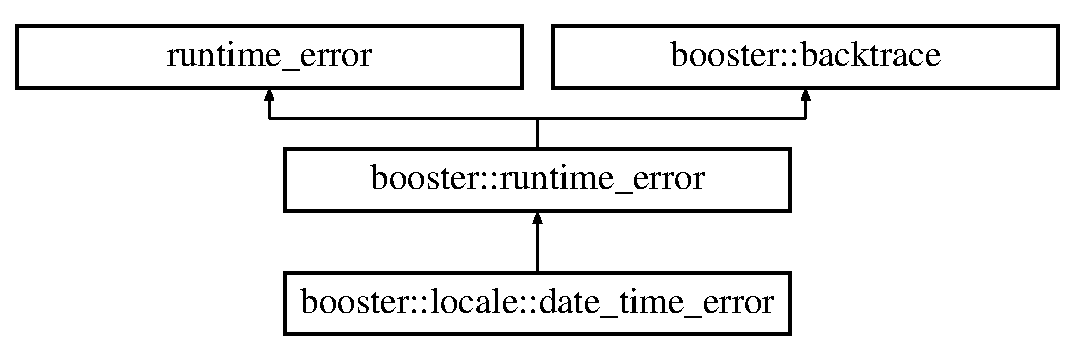
\includegraphics[height=3.000000cm]{classbooster_1_1locale_1_1date__time__error}
\end{center}
\end{figure}
\subsection*{Public Member Functions}
\begin{DoxyCompactItemize}
\item 
{\bf date\+\_\+time\+\_\+error} (std\+::string const \&e)
\end{DoxyCompactItemize}
\subsection*{Additional Inherited Members}


\subsection{Detailed Description}
This error is thrown in case of invalid state that occurred. 

\subsection{Constructor \& Destructor Documentation}
\index{booster\+::locale\+::date\+\_\+time\+\_\+error@{booster\+::locale\+::date\+\_\+time\+\_\+error}!date\+\_\+time\+\_\+error@{date\+\_\+time\+\_\+error}}
\index{date\+\_\+time\+\_\+error@{date\+\_\+time\+\_\+error}!booster\+::locale\+::date\+\_\+time\+\_\+error@{booster\+::locale\+::date\+\_\+time\+\_\+error}}
\subsubsection[{date\+\_\+time\+\_\+error(std\+::string const \&e)}]{\setlength{\rightskip}{0pt plus 5cm}booster\+::locale\+::date\+\_\+time\+\_\+error\+::date\+\_\+time\+\_\+error (
\begin{DoxyParamCaption}
\item[{std\+::string const \&}]{e}
\end{DoxyParamCaption}
)\hspace{0.3cm}{\ttfamily [inline]}}\label{classbooster_1_1locale_1_1date__time__error_aeff5ce5f1f201e26d804553bbb4f2fb3}
Constructor of \doxyref{date\+\_\+time\+\_\+error}{p.}{classbooster_1_1locale_1_1date__time__error} class 

The documentation for this class was generated from the following file\+:\begin{DoxyCompactItemize}
\item 
booster/locale/date\+\_\+time.\+h\end{DoxyCompactItemize}

\section{booster\+:\+:locale\+:\+:date\+\_\+time\+\_\+period Struct Reference}
\label{structbooster_1_1locale_1_1date__time__period}\index{booster\+::locale\+::date\+\_\+time\+\_\+period@{booster\+::locale\+::date\+\_\+time\+\_\+period}}


This class represents a pair of period\+\_\+type and the integer values that describes its amount. For example 3 days or 4 years.  




{\ttfamily \#include $<$booster/booster/locale/date\+\_\+time.\+h$>$}

\subsection*{Public Member Functions}
\begin{DoxyCompactItemize}
\item 
{\bf date\+\_\+time\+\_\+period} {\bf operator+} () const 
\item 
{\bf date\+\_\+time\+\_\+period} {\bf operator-\/} () const 
\item 
{\bf date\+\_\+time\+\_\+period} ({\bf period\+::period\+\_\+type} f={\bf period\+::period\+\_\+type}(), int v=1)
\end{DoxyCompactItemize}
\subsection*{Public Attributes}
\begin{DoxyCompactItemize}
\item 
{\bf period\+::period\+\_\+type} {\bf type}\label{structbooster_1_1locale_1_1date__time__period_a19fc27a6b8cb6946fd6dc4c57a0d0d50}

\begin{DoxyCompactList}\small\item\em The type of period, i.\+e. era, year, day etc. \end{DoxyCompactList}\item 
int {\bf value}
\end{DoxyCompactItemize}


\subsection{Detailed Description}
This class represents a pair of period\+\_\+type and the integer values that describes its amount. For example 3 days or 4 years. 

Usually obtained as product of period\+\_\+type and integer or my calling a representative functions For example day()$\ast$3 == date\+\_\+time\+\_\+period(day(),3) == day(3) 

\subsection{Constructor \& Destructor Documentation}
\index{booster\+::locale\+::date\+\_\+time\+\_\+period@{booster\+::locale\+::date\+\_\+time\+\_\+period}!date\+\_\+time\+\_\+period@{date\+\_\+time\+\_\+period}}
\index{date\+\_\+time\+\_\+period@{date\+\_\+time\+\_\+period}!booster\+::locale\+::date\+\_\+time\+\_\+period@{booster\+::locale\+::date\+\_\+time\+\_\+period}}
\subsubsection[{date\+\_\+time\+\_\+period(period\+::period\+\_\+type f=period\+::period\+\_\+type(), int v=1)}]{\setlength{\rightskip}{0pt plus 5cm}booster\+::locale\+::date\+\_\+time\+\_\+period\+::date\+\_\+time\+\_\+period (
\begin{DoxyParamCaption}
\item[{{\bf period\+::period\+\_\+type}}]{f = {\ttfamily {\bf period\+::period\+\_\+type}()}, }
\item[{int}]{v = {\ttfamily 1}}
\end{DoxyParamCaption}
)\hspace{0.3cm}{\ttfamily [inline]}}\label{structbooster_1_1locale_1_1date__time__period_a562a41045b0fd520f6d38b741efe2a99}
Constructor that creates \doxyref{date\+\_\+time\+\_\+period}{p.}{structbooster_1_1locale_1_1date__time__period} from period\+\_\+type {\itshape f} and a value {\itshape v} -- default 1. 

\subsection{Member Function Documentation}
\index{booster\+::locale\+::date\+\_\+time\+\_\+period@{booster\+::locale\+::date\+\_\+time\+\_\+period}!operator+@{operator+}}
\index{operator+@{operator+}!booster\+::locale\+::date\+\_\+time\+\_\+period@{booster\+::locale\+::date\+\_\+time\+\_\+period}}
\subsubsection[{operator+() const }]{\setlength{\rightskip}{0pt plus 5cm}{\bf date\+\_\+time\+\_\+period} booster\+::locale\+::date\+\_\+time\+\_\+period\+::operator+ (
\begin{DoxyParamCaption}
{}
\end{DoxyParamCaption}
) const\hspace{0.3cm}{\ttfamily [inline]}}\label{structbooster_1_1locale_1_1date__time__period_a0676f002c3342bb5ae042dc02156681b}
Operator + returns copy of itself \index{booster\+::locale\+::date\+\_\+time\+\_\+period@{booster\+::locale\+::date\+\_\+time\+\_\+period}!operator-\/@{operator-\/}}
\index{operator-\/@{operator-\/}!booster\+::locale\+::date\+\_\+time\+\_\+period@{booster\+::locale\+::date\+\_\+time\+\_\+period}}
\subsubsection[{operator-\/() const }]{\setlength{\rightskip}{0pt plus 5cm}{\bf date\+\_\+time\+\_\+period} booster\+::locale\+::date\+\_\+time\+\_\+period\+::operator-\/ (
\begin{DoxyParamCaption}
{}
\end{DoxyParamCaption}
) const\hspace{0.3cm}{\ttfamily [inline]}}\label{structbooster_1_1locale_1_1date__time__period_adaaf8c58b3d95a736bbabd34733de1d5}
Operator -\/, switches the sign of period 

\subsection{Member Data Documentation}
\index{booster\+::locale\+::date\+\_\+time\+\_\+period@{booster\+::locale\+::date\+\_\+time\+\_\+period}!value@{value}}
\index{value@{value}!booster\+::locale\+::date\+\_\+time\+\_\+period@{booster\+::locale\+::date\+\_\+time\+\_\+period}}
\subsubsection[{value}]{\setlength{\rightskip}{0pt plus 5cm}int booster\+::locale\+::date\+\_\+time\+\_\+period\+::value}\label{structbooster_1_1locale_1_1date__time__period_a3c5dd191feae2a75b52d143ad29a0cc1}
The value the actual number of {\itshape periods} 

Referenced by booster\+::locale\+::period\+::operator$\ast$().



The documentation for this struct was generated from the following file\+:\begin{DoxyCompactItemize}
\item 
booster/locale/date\+\_\+time.\+h\end{DoxyCompactItemize}

\section{booster\+:\+:locale\+:\+:date\+\_\+time\+\_\+period\+\_\+set Class Reference}
\label{classbooster_1_1locale_1_1date__time__period__set}\index{booster\+::locale\+::date\+\_\+time\+\_\+period\+\_\+set@{booster\+::locale\+::date\+\_\+time\+\_\+period\+\_\+set}}


this class that represents a set of periods,  




{\ttfamily \#include $<$booster/booster/locale/date\+\_\+time.\+h$>$}

\subsection*{Public Member Functions}
\begin{DoxyCompactItemize}
\item 
{\bf date\+\_\+time\+\_\+period\+\_\+set} ()
\item 
{\bf date\+\_\+time\+\_\+period\+\_\+set} ({\bf period\+::period\+\_\+type} f)
\item 
{\bf date\+\_\+time\+\_\+period\+\_\+set} ({\bf date\+\_\+time\+\_\+period} const \&fl)
\item 
void {\bf add} ({\bf date\+\_\+time\+\_\+period} f)
\item 
size\+\_\+t {\bf size} () const 
\item 
{\bf date\+\_\+time\+\_\+period} const \& {\bf operator[$\,$]} (size\+\_\+t n) const 
\end{DoxyCompactItemize}


\subsection{Detailed Description}
this class that represents a set of periods, 

It is generally created by operations on periods\+: 1995$\ast$year + 3$\ast$month + 1$\ast$day. Note\+: operations are not commutative. 

\subsection{Constructor \& Destructor Documentation}
\index{booster\+::locale\+::date\+\_\+time\+\_\+period\+\_\+set@{booster\+::locale\+::date\+\_\+time\+\_\+period\+\_\+set}!date\+\_\+time\+\_\+period\+\_\+set@{date\+\_\+time\+\_\+period\+\_\+set}}
\index{date\+\_\+time\+\_\+period\+\_\+set@{date\+\_\+time\+\_\+period\+\_\+set}!booster\+::locale\+::date\+\_\+time\+\_\+period\+\_\+set@{booster\+::locale\+::date\+\_\+time\+\_\+period\+\_\+set}}
\subsubsection[{date\+\_\+time\+\_\+period\+\_\+set()}]{\setlength{\rightskip}{0pt plus 5cm}booster\+::locale\+::date\+\_\+time\+\_\+period\+\_\+set\+::date\+\_\+time\+\_\+period\+\_\+set (
\begin{DoxyParamCaption}
{}
\end{DoxyParamCaption}
)\hspace{0.3cm}{\ttfamily [inline]}}\label{classbooster_1_1locale_1_1date__time__period__set_aa118edb2f0dd6012ba2ea2d690f0f71f}
Default constructor -\/ empty set \index{booster\+::locale\+::date\+\_\+time\+\_\+period\+\_\+set@{booster\+::locale\+::date\+\_\+time\+\_\+period\+\_\+set}!date\+\_\+time\+\_\+period\+\_\+set@{date\+\_\+time\+\_\+period\+\_\+set}}
\index{date\+\_\+time\+\_\+period\+\_\+set@{date\+\_\+time\+\_\+period\+\_\+set}!booster\+::locale\+::date\+\_\+time\+\_\+period\+\_\+set@{booster\+::locale\+::date\+\_\+time\+\_\+period\+\_\+set}}
\subsubsection[{date\+\_\+time\+\_\+period\+\_\+set(period\+::period\+\_\+type f)}]{\setlength{\rightskip}{0pt plus 5cm}booster\+::locale\+::date\+\_\+time\+\_\+period\+\_\+set\+::date\+\_\+time\+\_\+period\+\_\+set (
\begin{DoxyParamCaption}
\item[{{\bf period\+::period\+\_\+type}}]{f}
\end{DoxyParamCaption}
)\hspace{0.3cm}{\ttfamily [inline]}}\label{classbooster_1_1locale_1_1date__time__period__set_ae580201592e89ba073ea965e69135b53}
Create a set of single period with value 1 \index{booster\+::locale\+::date\+\_\+time\+\_\+period\+\_\+set@{booster\+::locale\+::date\+\_\+time\+\_\+period\+\_\+set}!date\+\_\+time\+\_\+period\+\_\+set@{date\+\_\+time\+\_\+period\+\_\+set}}
\index{date\+\_\+time\+\_\+period\+\_\+set@{date\+\_\+time\+\_\+period\+\_\+set}!booster\+::locale\+::date\+\_\+time\+\_\+period\+\_\+set@{booster\+::locale\+::date\+\_\+time\+\_\+period\+\_\+set}}
\subsubsection[{date\+\_\+time\+\_\+period\+\_\+set(date\+\_\+time\+\_\+period const \&fl)}]{\setlength{\rightskip}{0pt plus 5cm}booster\+::locale\+::date\+\_\+time\+\_\+period\+\_\+set\+::date\+\_\+time\+\_\+period\+\_\+set (
\begin{DoxyParamCaption}
\item[{{\bf date\+\_\+time\+\_\+period} const \&}]{fl}
\end{DoxyParamCaption}
)\hspace{0.3cm}{\ttfamily [inline]}}\label{classbooster_1_1locale_1_1date__time__period__set_a58606adb3f81eb5ee6b895ce718797ee}
Create a set of single period {\itshape fl} 

\subsection{Member Function Documentation}
\index{booster\+::locale\+::date\+\_\+time\+\_\+period\+\_\+set@{booster\+::locale\+::date\+\_\+time\+\_\+period\+\_\+set}!add@{add}}
\index{add@{add}!booster\+::locale\+::date\+\_\+time\+\_\+period\+\_\+set@{booster\+::locale\+::date\+\_\+time\+\_\+period\+\_\+set}}
\subsubsection[{add(date\+\_\+time\+\_\+period f)}]{\setlength{\rightskip}{0pt plus 5cm}void booster\+::locale\+::date\+\_\+time\+\_\+period\+\_\+set\+::add (
\begin{DoxyParamCaption}
\item[{{\bf date\+\_\+time\+\_\+period}}]{f}
\end{DoxyParamCaption}
)\hspace{0.3cm}{\ttfamily [inline]}}\label{classbooster_1_1locale_1_1date__time__period__set_a0b0ed8a1051da165a73687247b22cb44}
Append \doxyref{date\+\_\+time\+\_\+period}{p.}{structbooster_1_1locale_1_1date__time__period} {\itshape f} to the set 

Referenced by booster\+::locale\+::operator+(), and booster\+::locale\+::operator-\/().

\index{booster\+::locale\+::date\+\_\+time\+\_\+period\+\_\+set@{booster\+::locale\+::date\+\_\+time\+\_\+period\+\_\+set}!operator[$\,$]@{operator[]}}
\index{operator[$\,$]@{operator[]}!booster\+::locale\+::date\+\_\+time\+\_\+period\+\_\+set@{booster\+::locale\+::date\+\_\+time\+\_\+period\+\_\+set}}
\subsubsection[{operator[](size\+\_\+t n) const }]{\setlength{\rightskip}{0pt plus 5cm}{\bf date\+\_\+time\+\_\+period} const\& booster\+::locale\+::date\+\_\+time\+\_\+period\+\_\+set\+::operator[$\,$] (
\begin{DoxyParamCaption}
\item[{size\+\_\+t}]{n}
\end{DoxyParamCaption}
) const\hspace{0.3cm}{\ttfamily [inline]}}\label{classbooster_1_1locale_1_1date__time__period__set_a32f99861f9841e3f7f0f21554df4bea5}
Get item at position {\itshape n} the set, n should be in range [0,size) \index{booster\+::locale\+::date\+\_\+time\+\_\+period\+\_\+set@{booster\+::locale\+::date\+\_\+time\+\_\+period\+\_\+set}!size@{size}}
\index{size@{size}!booster\+::locale\+::date\+\_\+time\+\_\+period\+\_\+set@{booster\+::locale\+::date\+\_\+time\+\_\+period\+\_\+set}}
\subsubsection[{size() const }]{\setlength{\rightskip}{0pt plus 5cm}size\+\_\+t booster\+::locale\+::date\+\_\+time\+\_\+period\+\_\+set\+::size (
\begin{DoxyParamCaption}
{}
\end{DoxyParamCaption}
) const\hspace{0.3cm}{\ttfamily [inline]}}\label{classbooster_1_1locale_1_1date__time__period__set_ae17a871279b5645287399043466f124a}
Get number if items in list 

Referenced by booster\+::locale\+::operator+(), and booster\+::locale\+::operator-\/().



The documentation for this class was generated from the following file\+:\begin{DoxyCompactItemize}
\item 
booster/locale/date\+\_\+time.\+h\end{DoxyCompactItemize}

\section{cppcms\+:\+:filters\+:\+:datetime Class Reference}
\label{classcppcms_1_1filters_1_1datetime}\index{cppcms\+::filters\+::datetime@{cppcms\+::filters\+::datetime}}


Format date and time to ouput stream.  




{\ttfamily \#include $<$cppcms/filters.\+h$>$}

\subsection*{Public Member Functions}
\begin{DoxyCompactItemize}
\item 
{\bfseries datetime} ({\bf datetime} const \&other)\label{classcppcms_1_1filters_1_1datetime_a4c69cb76179ac3d2c535cd2d6887ba26}

\item 
{\bf datetime} const \& {\bfseries operator=} ({\bf datetime} const \&other)\label{classcppcms_1_1filters_1_1datetime_acb2d8eda9e9895feafe117ad003e7a44}

\item 
{\bf datetime} ({\bf streamable} const \&t)
\item 
{\bf datetime} ({\bf streamable} const \&{\bf time}, std\+::string const \&timezone)
\item 
void {\bfseries operator()} (std\+::ostream \&out) const \label{classcppcms_1_1filters_1_1datetime_a3abbf58652bed8ea9c641d08bd091d59}

\end{DoxyCompactItemize}


\subsection{Detailed Description}
Format date and time to ouput stream. 

Formats date and time to the stream, date and time is represented as time\+\_\+t 

\subsection{Constructor \& Destructor Documentation}
\index{cppcms\+::filters\+::datetime@{cppcms\+::filters\+::datetime}!datetime@{datetime}}
\index{datetime@{datetime}!cppcms\+::filters\+::datetime@{cppcms\+::filters\+::datetime}}
\subsubsection[{datetime(streamable const \&t)}]{\setlength{\rightskip}{0pt plus 5cm}cppcms\+::filters\+::datetime\+::datetime (
\begin{DoxyParamCaption}
\item[{{\bf streamable} const \&}]{t}
\end{DoxyParamCaption}
)}\label{classcppcms_1_1filters_1_1datetime_a8f514a9fd1c724441a3ffbb5fd3c0a63}
Create date and time filter that formats current local-\/time date and time using P\+O\+S\+IX time representation {\itshape t} \index{cppcms\+::filters\+::datetime@{cppcms\+::filters\+::datetime}!datetime@{datetime}}
\index{datetime@{datetime}!cppcms\+::filters\+::datetime@{cppcms\+::filters\+::datetime}}
\subsubsection[{datetime(streamable const \&time, std\+::string const \&timezone)}]{\setlength{\rightskip}{0pt plus 5cm}cppcms\+::filters\+::datetime\+::datetime (
\begin{DoxyParamCaption}
\item[{{\bf streamable} const \&}]{time, }
\item[{std\+::string const \&}]{timezone}
\end{DoxyParamCaption}
)}\label{classcppcms_1_1filters_1_1datetime_a250c6eedf8ac21addf46c37543ce4578}
Create date and time filter that formats current date and time using P\+O\+S\+IX time representation {\itshape t}, in a timezone {\itshape timezone} 

The documentation for this class was generated from the following file\+:\begin{DoxyCompactItemize}
\item 
cppcms/filters.\+h\end{DoxyCompactItemize}

\section{booster\+:\+:aio\+:\+:deadline\+\_\+timer Class Reference}
\label{classbooster_1_1aio_1_1deadline__timer}\index{booster\+::aio\+::deadline\+\_\+timer@{booster\+::aio\+::deadline\+\_\+timer}}


A timer object.  




{\ttfamily \#include $<$booster/booster/aio/deadline\+\_\+timer.\+h$>$}

Inheritance diagram for booster\+:\+:aio\+:\+:deadline\+\_\+timer\+:\begin{figure}[H]
\begin{center}
\leavevmode
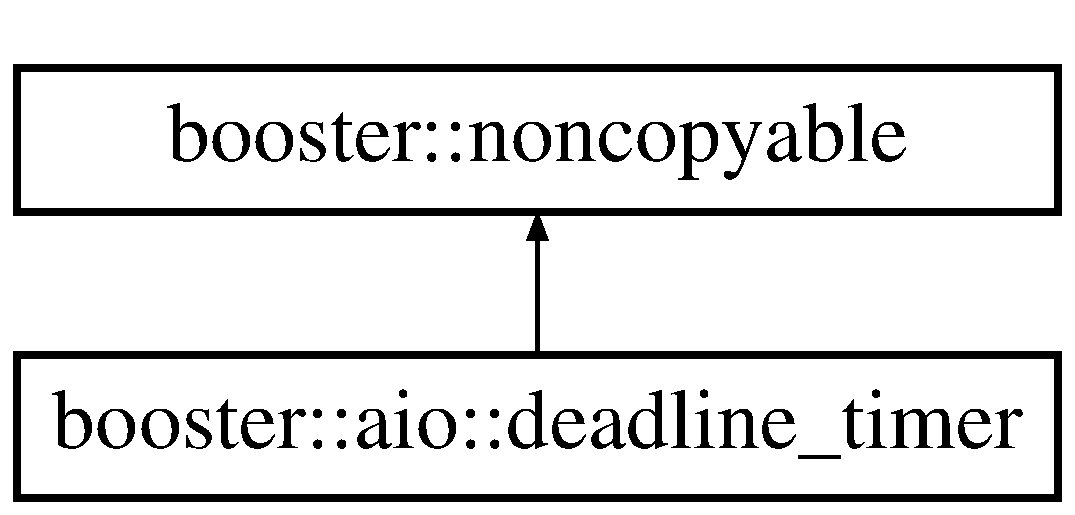
\includegraphics[height=2.000000cm]{classbooster_1_1aio_1_1deadline__timer}
\end{center}
\end{figure}
\subsection*{Public Member Functions}
\begin{DoxyCompactItemize}
\item 
{\bf deadline\+\_\+timer} ()
\item 
{\bf deadline\+\_\+timer} ({\bf io\+\_\+service} \&srv)
\item 
{\bf io\+\_\+service} \& {\bf get\+\_\+io\+\_\+service} ()
\item 
void {\bf set\+\_\+io\+\_\+service} ({\bf io\+\_\+service} \&srv)
\item 
void {\bf reset\+\_\+io\+\_\+service} ()
\item 
void {\bf expires\+\_\+from\+\_\+now} ({\bf ptime} t)
\item 
{\bf ptime} {\bf expires\+\_\+from\+\_\+now} ()
\item 
void {\bf expires\+\_\+at} ({\bf ptime} t)
\item 
{\bf ptime} {\bf expires\+\_\+at} ()
\item 
void {\bf wait} ()
\item 
void {\bf async\+\_\+wait} ({\bf event\+\_\+handler} const \&h)
\item 
void {\bf cancel} ()
\end{DoxyCompactItemize}
\subsection*{Friends}
\begin{DoxyCompactItemize}
\item 
struct {\bfseries waiter}\label{classbooster_1_1aio_1_1deadline__timer_a5c2d8ad3dc03a2fcae52cb8a99db61cc}

\end{DoxyCompactItemize}


\subsection{Detailed Description}
A timer object. 

\subsection{Constructor \& Destructor Documentation}
\index{booster\+::aio\+::deadline\+\_\+timer@{booster\+::aio\+::deadline\+\_\+timer}!deadline\+\_\+timer@{deadline\+\_\+timer}}
\index{deadline\+\_\+timer@{deadline\+\_\+timer}!booster\+::aio\+::deadline\+\_\+timer@{booster\+::aio\+::deadline\+\_\+timer}}
\subsubsection[{deadline\+\_\+timer()}]{\setlength{\rightskip}{0pt plus 5cm}booster\+::aio\+::deadline\+\_\+timer\+::deadline\+\_\+timer (
\begin{DoxyParamCaption}
{}
\end{DoxyParamCaption}
)}\label{classbooster_1_1aio_1_1deadline__timer_a10c5a351425da3102852dd5749d1d2b0}
Create a new timer object \index{booster\+::aio\+::deadline\+\_\+timer@{booster\+::aio\+::deadline\+\_\+timer}!deadline\+\_\+timer@{deadline\+\_\+timer}}
\index{deadline\+\_\+timer@{deadline\+\_\+timer}!booster\+::aio\+::deadline\+\_\+timer@{booster\+::aio\+::deadline\+\_\+timer}}
\subsubsection[{deadline\+\_\+timer(io\+\_\+service \&srv)}]{\setlength{\rightskip}{0pt plus 5cm}booster\+::aio\+::deadline\+\_\+timer\+::deadline\+\_\+timer (
\begin{DoxyParamCaption}
\item[{{\bf io\+\_\+service} \&}]{srv}
\end{DoxyParamCaption}
)}\label{classbooster_1_1aio_1_1deadline__timer_af5421f825484cd6928faed18c161a56f}
Create a new timer object connected to the \doxyref{io\+\_\+service}{p.}{classbooster_1_1aio_1_1io__service} {\itshape srv} 

\subsection{Member Function Documentation}
\index{booster\+::aio\+::deadline\+\_\+timer@{booster\+::aio\+::deadline\+\_\+timer}!async\+\_\+wait@{async\+\_\+wait}}
\index{async\+\_\+wait@{async\+\_\+wait}!booster\+::aio\+::deadline\+\_\+timer@{booster\+::aio\+::deadline\+\_\+timer}}
\subsubsection[{async\+\_\+wait(event\+\_\+handler const \&h)}]{\setlength{\rightskip}{0pt plus 5cm}void booster\+::aio\+::deadline\+\_\+timer\+::async\+\_\+wait (
\begin{DoxyParamCaption}
\item[{{\bf event\+\_\+handler} const \&}]{h}
\end{DoxyParamCaption}
)}\label{classbooster_1_1aio_1_1deadline__timer_a792d60c0eb9f04d3f3a4bf54e6583c5c}
Wait asynchronously for the timer.

If \doxyref{io\+\_\+service}{p.}{classbooster_1_1aio_1_1io__service} is not assigned throws system\+::system\+\_\+error, all other errors reported via {\itshape h} \index{booster\+::aio\+::deadline\+\_\+timer@{booster\+::aio\+::deadline\+\_\+timer}!cancel@{cancel}}
\index{cancel@{cancel}!booster\+::aio\+::deadline\+\_\+timer@{booster\+::aio\+::deadline\+\_\+timer}}
\subsubsection[{cancel()}]{\setlength{\rightskip}{0pt plus 5cm}void booster\+::aio\+::deadline\+\_\+timer\+::cancel (
\begin{DoxyParamCaption}
{}
\end{DoxyParamCaption}
)}\label{classbooster_1_1aio_1_1deadline__timer_a056b1472d6c76b9688f6d94240695d26}
Cancel asynchronous operation. The active handler is immediately scheduled for execution with booster\+::aio\+::aio\+\_\+error\+::cancel error code in \doxyref{booster\+::aio\+::aio\+\_\+error\+\_\+cat}{p.}{namespacebooster_1_1aio_ab8fc36f5ba7b98b52f4082a85d3db8c9} category.

It allows to distinguish between operation cancellation and normal completion \index{booster\+::aio\+::deadline\+\_\+timer@{booster\+::aio\+::deadline\+\_\+timer}!expires\+\_\+at@{expires\+\_\+at}}
\index{expires\+\_\+at@{expires\+\_\+at}!booster\+::aio\+::deadline\+\_\+timer@{booster\+::aio\+::deadline\+\_\+timer}}
\subsubsection[{expires\+\_\+at(ptime t)}]{\setlength{\rightskip}{0pt plus 5cm}void booster\+::aio\+::deadline\+\_\+timer\+::expires\+\_\+at (
\begin{DoxyParamCaption}
\item[{{\bf ptime}}]{t}
\end{DoxyParamCaption}
)}\label{classbooster_1_1aio_1_1deadline__timer_a4b581b931e0f9cb1039e54b795d6baf1}
Set an absolute expiration time

If the function is called during the wait operation the behavior is undefined \index{booster\+::aio\+::deadline\+\_\+timer@{booster\+::aio\+::deadline\+\_\+timer}!expires\+\_\+at@{expires\+\_\+at}}
\index{expires\+\_\+at@{expires\+\_\+at}!booster\+::aio\+::deadline\+\_\+timer@{booster\+::aio\+::deadline\+\_\+timer}}
\subsubsection[{expires\+\_\+at()}]{\setlength{\rightskip}{0pt plus 5cm}{\bf ptime} booster\+::aio\+::deadline\+\_\+timer\+::expires\+\_\+at (
\begin{DoxyParamCaption}
{}
\end{DoxyParamCaption}
)}\label{classbooster_1_1aio_1_1deadline__timer_ae465226b8b180698d640cbf40e9d5628}
Get an absolute expiration time \index{booster\+::aio\+::deadline\+\_\+timer@{booster\+::aio\+::deadline\+\_\+timer}!expires\+\_\+from\+\_\+now@{expires\+\_\+from\+\_\+now}}
\index{expires\+\_\+from\+\_\+now@{expires\+\_\+from\+\_\+now}!booster\+::aio\+::deadline\+\_\+timer@{booster\+::aio\+::deadline\+\_\+timer}}
\subsubsection[{expires\+\_\+from\+\_\+now(ptime t)}]{\setlength{\rightskip}{0pt plus 5cm}void booster\+::aio\+::deadline\+\_\+timer\+::expires\+\_\+from\+\_\+now (
\begin{DoxyParamCaption}
\item[{{\bf ptime}}]{t}
\end{DoxyParamCaption}
)}\label{classbooster_1_1aio_1_1deadline__timer_a83e31e7cd377e0167c0ba5e4e04abe28}
Set an expiration time relativelty to the current point with an offset {\itshape t} 

If the function is called during the wait operation the behavior is undefined \index{booster\+::aio\+::deadline\+\_\+timer@{booster\+::aio\+::deadline\+\_\+timer}!expires\+\_\+from\+\_\+now@{expires\+\_\+from\+\_\+now}}
\index{expires\+\_\+from\+\_\+now@{expires\+\_\+from\+\_\+now}!booster\+::aio\+::deadline\+\_\+timer@{booster\+::aio\+::deadline\+\_\+timer}}
\subsubsection[{expires\+\_\+from\+\_\+now()}]{\setlength{\rightskip}{0pt plus 5cm}{\bf ptime} booster\+::aio\+::deadline\+\_\+timer\+::expires\+\_\+from\+\_\+now (
\begin{DoxyParamCaption}
{}
\end{DoxyParamCaption}
)}\label{classbooster_1_1aio_1_1deadline__timer_a92a91be95e439c8e367fa7883801ab86}
Get an expiration time relativelty to the current point with an offset {\itshape t} \index{booster\+::aio\+::deadline\+\_\+timer@{booster\+::aio\+::deadline\+\_\+timer}!get\+\_\+io\+\_\+service@{get\+\_\+io\+\_\+service}}
\index{get\+\_\+io\+\_\+service@{get\+\_\+io\+\_\+service}!booster\+::aio\+::deadline\+\_\+timer@{booster\+::aio\+::deadline\+\_\+timer}}
\subsubsection[{get\+\_\+io\+\_\+service()}]{\setlength{\rightskip}{0pt plus 5cm}{\bf io\+\_\+service}\& booster\+::aio\+::deadline\+\_\+timer\+::get\+\_\+io\+\_\+service (
\begin{DoxyParamCaption}
{}
\end{DoxyParamCaption}
)}\label{classbooster_1_1aio_1_1deadline__timer_af38f6201fba327069f89292839d42bf2}
Returns the connected \doxyref{io\+\_\+service}{p.}{classbooster_1_1aio_1_1io__service}, throws system\+::system\+\_\+error if no \doxyref{io\+\_\+service}{p.}{classbooster_1_1aio_1_1io__service} connected \index{booster\+::aio\+::deadline\+\_\+timer@{booster\+::aio\+::deadline\+\_\+timer}!reset\+\_\+io\+\_\+service@{reset\+\_\+io\+\_\+service}}
\index{reset\+\_\+io\+\_\+service@{reset\+\_\+io\+\_\+service}!booster\+::aio\+::deadline\+\_\+timer@{booster\+::aio\+::deadline\+\_\+timer}}
\subsubsection[{reset\+\_\+io\+\_\+service()}]{\setlength{\rightskip}{0pt plus 5cm}void booster\+::aio\+::deadline\+\_\+timer\+::reset\+\_\+io\+\_\+service (
\begin{DoxyParamCaption}
{}
\end{DoxyParamCaption}
)}\label{classbooster_1_1aio_1_1deadline__timer_a38864af40a6153479fbd1b0874d5b180}
Unsets the \doxyref{io\+\_\+service}{p.}{classbooster_1_1aio_1_1io__service}. Cancels all pending asynchronous operations on the connected \doxyref{io\+\_\+service}{p.}{classbooster_1_1aio_1_1io__service}. \index{booster\+::aio\+::deadline\+\_\+timer@{booster\+::aio\+::deadline\+\_\+timer}!set\+\_\+io\+\_\+service@{set\+\_\+io\+\_\+service}}
\index{set\+\_\+io\+\_\+service@{set\+\_\+io\+\_\+service}!booster\+::aio\+::deadline\+\_\+timer@{booster\+::aio\+::deadline\+\_\+timer}}
\subsubsection[{set\+\_\+io\+\_\+service(io\+\_\+service \&srv)}]{\setlength{\rightskip}{0pt plus 5cm}void booster\+::aio\+::deadline\+\_\+timer\+::set\+\_\+io\+\_\+service (
\begin{DoxyParamCaption}
\item[{{\bf io\+\_\+service} \&}]{srv}
\end{DoxyParamCaption}
)}\label{classbooster_1_1aio_1_1deadline__timer_aee4978be7d5c43cd4627a16df6b7da69}
Sets new \doxyref{io\+\_\+service}{p.}{classbooster_1_1aio_1_1io__service}. Cancels all pending asynchronous operations on the connected \doxyref{io\+\_\+service}{p.}{classbooster_1_1aio_1_1io__service}. \index{booster\+::aio\+::deadline\+\_\+timer@{booster\+::aio\+::deadline\+\_\+timer}!wait@{wait}}
\index{wait@{wait}!booster\+::aio\+::deadline\+\_\+timer@{booster\+::aio\+::deadline\+\_\+timer}}
\subsubsection[{wait()}]{\setlength{\rightskip}{0pt plus 5cm}void booster\+::aio\+::deadline\+\_\+timer\+::wait (
\begin{DoxyParamCaption}
{}
\end{DoxyParamCaption}
)}\label{classbooster_1_1aio_1_1deadline__timer_a4f22f7875d1ae32af184937456a5f084}
Wait synchronously for the timer 

The documentation for this class was generated from the following file\+:\begin{DoxyCompactItemize}
\item 
booster/aio/deadline\+\_\+timer.\+h\end{DoxyCompactItemize}

\section{booster\+:\+:locale\+:\+:gnu\+\_\+gettext\+:\+:messages\+\_\+info\+:\+:domain Struct Reference}
\label{structbooster_1_1locale_1_1gnu__gettext_1_1messages__info_1_1domain}\index{booster\+::locale\+::gnu\+\_\+gettext\+::messages\+\_\+info\+::domain@{booster\+::locale\+::gnu\+\_\+gettext\+::messages\+\_\+info\+::domain}}


This type represents G\+NU Gettext domain name for the messages.  




{\ttfamily \#include $<$booster/booster/locale/gnu\+\_\+gettext.\+h$>$}

\subsection*{Public Member Functions}
\begin{DoxyCompactItemize}
\item 
{\bf domain} (std\+::string const \&n)
\item 
bool {\bf operator==} ({\bf domain} const \&other) const 
\item 
bool {\bf operator!=} ({\bf domain} const \&other) const 
\end{DoxyCompactItemize}
\subsection*{Public Attributes}
\begin{DoxyCompactItemize}
\item 
std\+::string {\bf name}\label{structbooster_1_1locale_1_1gnu__gettext_1_1messages__info_1_1domain_ab32a01da627a4a09b1b202d3b1300445}

\begin{DoxyCompactList}\small\item\em The name of the domain. \end{DoxyCompactList}\item 
std\+::string {\bf encoding}\label{structbooster_1_1locale_1_1gnu__gettext_1_1messages__info_1_1domain_abd80ccbde7068ceffcfc7a5864b1a744}

\begin{DoxyCompactList}\small\item\em The character encoding for the domain. \end{DoxyCompactList}\end{DoxyCompactItemize}


\subsection{Detailed Description}
This type represents G\+NU Gettext domain name for the messages. 

It consists of two parameters\+:


\begin{DoxyItemize}
\item name -\/ the name of the domain -\/ used for opening the file name
\item encoding -\/ the encoding of the keys in the sources, default -\/ U\+T\+F-\/8 
\end{DoxyItemize}

\subsection{Constructor \& Destructor Documentation}
\index{booster\+::locale\+::gnu\+\_\+gettext\+::messages\+\_\+info\+::domain@{booster\+::locale\+::gnu\+\_\+gettext\+::messages\+\_\+info\+::domain}!domain@{domain}}
\index{domain@{domain}!booster\+::locale\+::gnu\+\_\+gettext\+::messages\+\_\+info\+::domain@{booster\+::locale\+::gnu\+\_\+gettext\+::messages\+\_\+info\+::domain}}
\subsubsection[{domain(std\+::string const \&n)}]{\setlength{\rightskip}{0pt plus 5cm}booster\+::locale\+::gnu\+\_\+gettext\+::messages\+\_\+info\+::domain\+::domain (
\begin{DoxyParamCaption}
\item[{std\+::string const \&}]{n}
\end{DoxyParamCaption}
)\hspace{0.3cm}{\ttfamily [inline]}}\label{structbooster_1_1locale_1_1gnu__gettext_1_1messages__info_1_1domain_a370acf3762cf19dc9546b87486b2e53e}
Create a domain object from the name that can hold an encoding after symbol \char`\"{}/\char`\"{} such that if n is \char`\"{}hello/cp1255\char`\"{} then the name would be \char`\"{}hello\char`\"{} and \char`\"{}encoding\char`\"{} would be \char`\"{}cp1255\char`\"{} and if n is \char`\"{}hello\char`\"{} then the name would be the same but encoding would be \char`\"{}\+U\+T\+F-\/8\char`\"{} 

\subsection{Member Function Documentation}
\index{booster\+::locale\+::gnu\+\_\+gettext\+::messages\+\_\+info\+::domain@{booster\+::locale\+::gnu\+\_\+gettext\+::messages\+\_\+info\+::domain}!operator"!=@{operator"!=}}
\index{operator"!=@{operator"!=}!booster\+::locale\+::gnu\+\_\+gettext\+::messages\+\_\+info\+::domain@{booster\+::locale\+::gnu\+\_\+gettext\+::messages\+\_\+info\+::domain}}
\subsubsection[{operator"!=(domain const \&other) const }]{\setlength{\rightskip}{0pt plus 5cm}bool booster\+::locale\+::gnu\+\_\+gettext\+::messages\+\_\+info\+::domain\+::operator!= (
\begin{DoxyParamCaption}
\item[{{\bf domain} const \&}]{other}
\end{DoxyParamCaption}
) const\hspace{0.3cm}{\ttfamily [inline]}}\label{structbooster_1_1locale_1_1gnu__gettext_1_1messages__info_1_1domain_afe58497d272f37848eb5f186e1ab1ab9}
Check whether two objects are distinct, only names are compared, encoding is ignored \index{booster\+::locale\+::gnu\+\_\+gettext\+::messages\+\_\+info\+::domain@{booster\+::locale\+::gnu\+\_\+gettext\+::messages\+\_\+info\+::domain}!operator==@{operator==}}
\index{operator==@{operator==}!booster\+::locale\+::gnu\+\_\+gettext\+::messages\+\_\+info\+::domain@{booster\+::locale\+::gnu\+\_\+gettext\+::messages\+\_\+info\+::domain}}
\subsubsection[{operator==(domain const \&other) const }]{\setlength{\rightskip}{0pt plus 5cm}bool booster\+::locale\+::gnu\+\_\+gettext\+::messages\+\_\+info\+::domain\+::operator== (
\begin{DoxyParamCaption}
\item[{{\bf domain} const \&}]{other}
\end{DoxyParamCaption}
) const\hspace{0.3cm}{\ttfamily [inline]}}\label{structbooster_1_1locale_1_1gnu__gettext_1_1messages__info_1_1domain_a7f9f0c06978b4ac52dc12e6119d16eaa}
Check whether two objects are equivalent, only names are compared, encoding is ignored 

References name.



The documentation for this struct was generated from the following file\+:\begin{DoxyCompactItemize}
\item 
booster/locale/gnu\+\_\+gettext.\+h\end{DoxyCompactItemize}

\section{booster\+:\+:domain\+\_\+error Class Reference}
\label{classbooster_1_1domain__error}\index{booster\+::domain\+\_\+error@{booster\+::domain\+\_\+error}}


Same as std\+::domain\+\_\+error but records stack trace.  




{\ttfamily \#include $<$booster/booster/backtrace.\+h$>$}

Inheritance diagram for booster\+:\+:domain\+\_\+error\+:\begin{figure}[H]
\begin{center}
\leavevmode
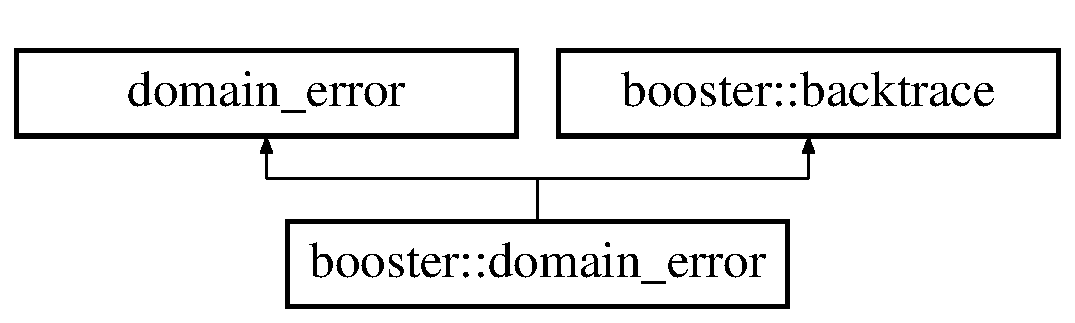
\includegraphics[height=2.000000cm]{classbooster_1_1domain__error}
\end{center}
\end{figure}
\subsection*{Public Member Functions}
\begin{DoxyCompactItemize}
\item 
{\bfseries domain\+\_\+error} (std\+::string const \&s)\label{classbooster_1_1domain__error_a06047ee402ac045abc0b6c3ef432ea06}

\end{DoxyCompactItemize}
\subsection*{Additional Inherited Members}


\subsection{Detailed Description}
Same as std\+::domain\+\_\+error but records stack trace. 

The documentation for this class was generated from the following file\+:\begin{DoxyCompactItemize}
\item 
booster/backtrace.\+h\end{DoxyCompactItemize}

\section{cppcms\+:\+:widgets\+:\+:select\+\_\+base\+:\+:element Struct Reference}
\label{structcppcms_1_1widgets_1_1select__base_1_1element}\index{cppcms\+::widgets\+::select\+\_\+base\+::element@{cppcms\+::widgets\+::select\+\_\+base\+::element}}
\subsection*{Public Member Functions}
\begin{DoxyCompactItemize}
\item 
{\bfseries element} (std\+::string const \&v, {\bf locale\+::message} const \&msg)\label{structcppcms_1_1widgets_1_1select__base_1_1element_a2201a008a67419d33ddc6c141543ed6e}

\item 
{\bfseries element} (std\+::string const \&v, std\+::string const \&msg)\label{structcppcms_1_1widgets_1_1select__base_1_1element_a6a575261395968caa7086aaad3c7322c}

\item 
{\bfseries element} ({\bf element} const \&)\label{structcppcms_1_1widgets_1_1select__base_1_1element_a5cbd376bab3bc8c9efe56d4c41bf326f}

\item 
{\bf element} const \& {\bfseries operator=} ({\bf element} const \&)\label{structcppcms_1_1widgets_1_1select__base_1_1element_a5b9a12b09adef1c19ead2de703c26c59}

\end{DoxyCompactItemize}
\subsection*{Public Attributes}
\begin{DoxyCompactItemize}
\item 
uint32\+\_\+t {\bfseries need\+\_\+translation}\+: 1\label{structcppcms_1_1widgets_1_1select__base_1_1element_ac4a47dc24f69edf6aa32a34cf6040d7e}

\item 
C\+P\+P\+C\+M\+S\+\_\+\+U\+N\+U\+S\+E\+D\+\_\+\+M\+E\+M\+B\+ER uint32\+\_\+t {\bfseries reserved}\+: 31\label{structcppcms_1_1widgets_1_1select__base_1_1element_a0f31afbd3776e21c5dc7deb79047ddd2}

\item 
std\+::string {\bfseries id}\label{structcppcms_1_1widgets_1_1select__base_1_1element_adc7a822a128e5a77ef0dffa3c9bb1157}

\item 
std\+::string {\bfseries str\+\_\+option}\label{structcppcms_1_1widgets_1_1select__base_1_1element_a05a50952d7a19286f8fb671631b6983b}

\item 
{\bf locale\+::message} {\bfseries tr\+\_\+option}\label{structcppcms_1_1widgets_1_1select__base_1_1element_a81d4cfcdae5c17b6020bfbbfacc58e57}

\end{DoxyCompactItemize}


The documentation for this struct was generated from the following file\+:\begin{DoxyCompactItemize}
\item 
cppcms/form.\+h\end{DoxyCompactItemize}

\section{cppcms\+:\+:widgets\+:\+:email Class Reference}
\label{classcppcms_1_1widgets_1_1email}\index{cppcms\+::widgets\+::email@{cppcms\+::widgets\+::email}}


This widget checks that the input is a valid email address.  




{\ttfamily \#include $<$cppcms/form.\+h$>$}

Inheritance diagram for cppcms\+:\+:widgets\+:\+:email\+:\begin{figure}[H]
\begin{center}
\leavevmode
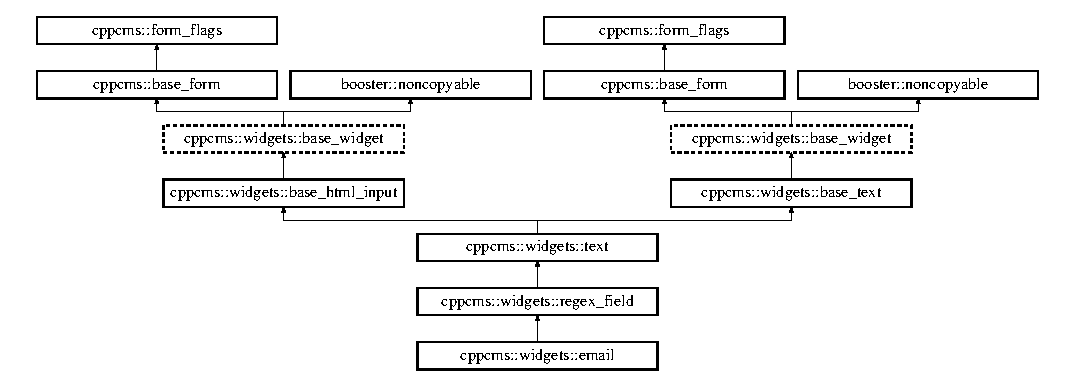
\includegraphics[height=4.734299cm]{classcppcms_1_1widgets_1_1email}
\end{center}
\end{figure}
\subsection*{Additional Inherited Members}


\subsection{Detailed Description}
This widget checks that the input is a valid email address. 

The documentation for this class was generated from the following file\+:\begin{DoxyCompactItemize}
\item 
cppcms/form.\+h\end{DoxyCompactItemize}

\section{cppcms\+:\+:sessions\+:\+:encryptor Class Reference}
\label{classcppcms_1_1sessions_1_1encryptor}\index{cppcms\+::sessions\+::encryptor@{cppcms\+::sessions\+::encryptor}}


This is an interface to generic session cookies encryption or signing A\+PI.  




{\ttfamily \#include $<$cppcms/session\+\_\+cookies.\+h$>$}

Inheritance diagram for cppcms\+:\+:sessions\+:\+:encryptor\+:\begin{figure}[H]
\begin{center}
\leavevmode
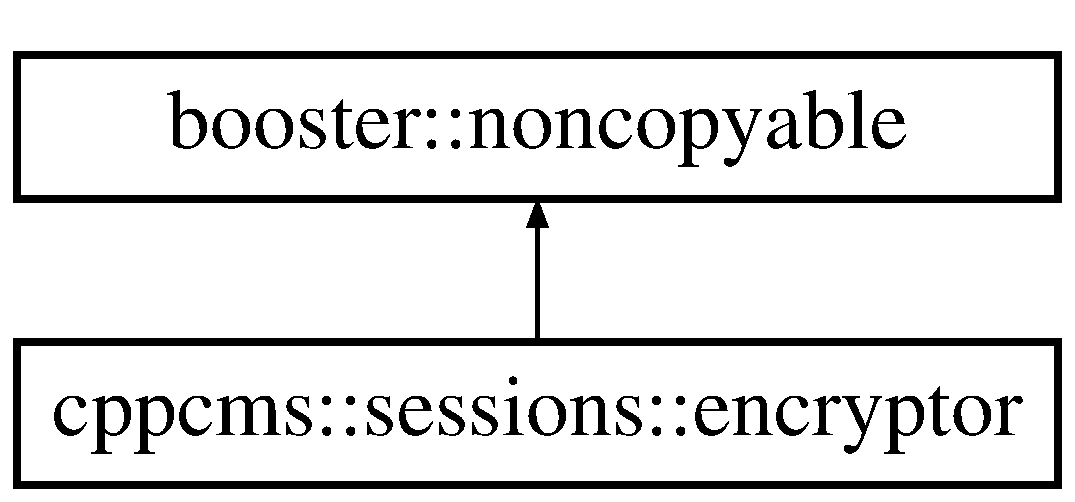
\includegraphics[height=2.000000cm]{classcppcms_1_1sessions_1_1encryptor}
\end{center}
\end{figure}
\subsection*{Public Member Functions}
\begin{DoxyCompactItemize}
\item 
virtual std\+::string {\bf encrypt} (std\+::string const \&plain)=0
\item 
virtual bool {\bf decrypt} (std\+::string const \&cipher, std\+::string \&plain)=0
\item 
virtual {\bf $\sim$encryptor} ()
\end{DoxyCompactItemize}


\subsection{Detailed Description}
This is an interface to generic session cookies encryption or signing A\+PI. 

Note for users implementing their own ecryptor classes\+:


\begin{DoxyItemize}
\item Be super paranoid and extremely careful in what you are doing.
\item Take in mind that this object are created and destroyed much frequently then they are actually accessed, so lazy initialization is your best friend.
\end{DoxyItemize}

Note this class does not have to be thread safe to use from multiple threads. 

\subsection{Constructor \& Destructor Documentation}
\index{cppcms\+::sessions\+::encryptor@{cppcms\+::sessions\+::encryptor}!````~encryptor@{$\sim$encryptor}}
\index{````~encryptor@{$\sim$encryptor}!cppcms\+::sessions\+::encryptor@{cppcms\+::sessions\+::encryptor}}
\subsubsection[{$\sim$encryptor()}]{\setlength{\rightskip}{0pt plus 5cm}virtual cppcms\+::sessions\+::encryptor\+::$\sim$encryptor (
\begin{DoxyParamCaption}
{}
\end{DoxyParamCaption}
)\hspace{0.3cm}{\ttfamily [inline]}, {\ttfamily [virtual]}}\label{classcppcms_1_1sessions_1_1encryptor_a045dc6fa8a3f7b9c15e1c181b7d7643e}
Destructor 

\subsection{Member Function Documentation}
\index{cppcms\+::sessions\+::encryptor@{cppcms\+::sessions\+::encryptor}!decrypt@{decrypt}}
\index{decrypt@{decrypt}!cppcms\+::sessions\+::encryptor@{cppcms\+::sessions\+::encryptor}}
\subsubsection[{decrypt(std\+::string const \&cipher, std\+::string \&plain)=0}]{\setlength{\rightskip}{0pt plus 5cm}virtual bool cppcms\+::sessions\+::encryptor\+::decrypt (
\begin{DoxyParamCaption}
\item[{std\+::string const \&}]{cipher, }
\item[{std\+::string \&}]{plain}
\end{DoxyParamCaption}
)\hspace{0.3cm}{\ttfamily [pure virtual]}}\label{classcppcms_1_1sessions_1_1encryptor_a79d46b6fe1b5b252245157d2d0a44670}
Decrypt the {\itshape cipher} text or check the signature and return the {\itshape plain} text and the session expiration value\+: {\itshape timeout}.

If signature checks or decryption failed return false. \index{cppcms\+::sessions\+::encryptor@{cppcms\+::sessions\+::encryptor}!encrypt@{encrypt}}
\index{encrypt@{encrypt}!cppcms\+::sessions\+::encryptor@{cppcms\+::sessions\+::encryptor}}
\subsubsection[{encrypt(std\+::string const \&plain)=0}]{\setlength{\rightskip}{0pt plus 5cm}virtual std\+::string cppcms\+::sessions\+::encryptor\+::encrypt (
\begin{DoxyParamCaption}
\item[{std\+::string const \&}]{plain}
\end{DoxyParamCaption}
)\hspace{0.3cm}{\ttfamily [pure virtual]}}\label{classcppcms_1_1sessions_1_1encryptor_adfaac1dbc3173e15c2c147b6d37480be}
Encrypt or sign the plain text {\itshape plain} together with {\itshape timeout} and return the encrypted value for a cookie. Don\textquotesingle{}t forget to use base64 encoding in order to create a string that is valid for cookie 

The documentation for this class was generated from the following file\+:\begin{DoxyCompactItemize}
\item 
cppcms/session\+\_\+cookies.\+h\end{DoxyCompactItemize}

\section{cppcms\+:\+:sessions\+:\+:encryptor\+\_\+factory Class Reference}
\label{classcppcms_1_1sessions_1_1encryptor__factory}\index{cppcms\+::sessions\+::encryptor\+\_\+factory@{cppcms\+::sessions\+::encryptor\+\_\+factory}}


This is an interface for an object that creates new encryptors.  




{\ttfamily \#include $<$cppcms/session\+\_\+cookies.\+h$>$}

\subsection*{Public Member Functions}
\begin{DoxyCompactItemize}
\item 
virtual std\+::unique\+\_\+ptr$<$ {\bf encryptor} $>$ {\bf get} ()=0
\item 
virtual {\bf $\sim$encryptor\+\_\+factory} ()
\end{DoxyCompactItemize}


\subsection{Detailed Description}
This is an interface for an object that creates new encryptors. 

This class must be thread safe. 

\subsection{Constructor \& Destructor Documentation}
\index{cppcms\+::sessions\+::encryptor\+\_\+factory@{cppcms\+::sessions\+::encryptor\+\_\+factory}!````~encryptor\+\_\+factory@{$\sim$encryptor\+\_\+factory}}
\index{````~encryptor\+\_\+factory@{$\sim$encryptor\+\_\+factory}!cppcms\+::sessions\+::encryptor\+\_\+factory@{cppcms\+::sessions\+::encryptor\+\_\+factory}}
\subsubsection[{$\sim$encryptor\+\_\+factory()}]{\setlength{\rightskip}{0pt plus 5cm}virtual cppcms\+::sessions\+::encryptor\+\_\+factory\+::$\sim$encryptor\+\_\+factory (
\begin{DoxyParamCaption}
{}
\end{DoxyParamCaption}
)\hspace{0.3cm}{\ttfamily [inline]}, {\ttfamily [virtual]}}\label{classcppcms_1_1sessions_1_1encryptor__factory_a218ecc309922e59dc8f8db57b87182ed}
Destructor -\/ cleanup everything 

\subsection{Member Function Documentation}
\index{cppcms\+::sessions\+::encryptor\+\_\+factory@{cppcms\+::sessions\+::encryptor\+\_\+factory}!get@{get}}
\index{get@{get}!cppcms\+::sessions\+::encryptor\+\_\+factory@{cppcms\+::sessions\+::encryptor\+\_\+factory}}
\subsubsection[{get()=0}]{\setlength{\rightskip}{0pt plus 5cm}virtual std\+::unique\+\_\+ptr$<${\bf encryptor}$>$ cppcms\+::sessions\+::encryptor\+\_\+factory\+::get (
\begin{DoxyParamCaption}
{}
\end{DoxyParamCaption}
)\hspace{0.3cm}{\ttfamily [pure virtual]}}\label{classcppcms_1_1sessions_1_1encryptor__factory_ad25bf8b34833b1292136c61b87982de6}
Return a pointer to a newly created encryptor. 

The documentation for this class was generated from the following file\+:\begin{DoxyCompactItemize}
\item 
cppcms/session\+\_\+cookies.\+h\end{DoxyCompactItemize}

\section{booster\+:\+:aio\+:\+:endpoint Class Reference}
\label{classbooster_1_1aio_1_1endpoint}\index{booster\+::aio\+::endpoint@{booster\+::aio\+::endpoint}}


this class represents the connection endpoint, that is generally sockaddr structure in Berkeley sockets A\+PI.  




{\ttfamily \#include $<$booster/booster/aio/endpoint.\+h$>$}

\subsection*{Public Types}
\begin{DoxyCompactItemize}
\item 
typedef std\+::pair$<$ sockaddr const $\ast$, int $>$ {\bf native\+\_\+address\+\_\+type}
\end{DoxyCompactItemize}
\subsection*{Public Member Functions}
\begin{DoxyCompactItemize}
\item 
{\bfseries endpoint} ({\bf endpoint} const \&)\label{classbooster_1_1aio_1_1endpoint_ae1799d20f79db212429f0340219d2330}

\item 
{\bf endpoint} const \& {\bfseries operator=} ({\bf endpoint} const \&)\label{classbooster_1_1aio_1_1endpoint_afe01e7f2f33961141d32e341c4aba36f}

\item 
{\bf endpoint} (std\+::string const \&{\bf ip}, int {\bf port})
\item 
void {\bf ip} (std\+::string const \&)
\item 
void {\bf port} (int)
\item 
std\+::string {\bf ip} () const 
\item 
int {\bf port} () const 
\item 
{\bf endpoint} (std\+::string const \&)
\item 
void {\bf path} (std\+::string const \&)
\item 
std\+::string {\bf path} () const 
\item 
{\bf family\+\_\+type} {\bf family} () const 
\item 
void {\bf raw} (sockaddr const $\ast$p, int size)
\item 
{\bf native\+\_\+address\+\_\+type} {\bf raw} () const 
\end{DoxyCompactItemize}


\subsection{Detailed Description}
this class represents the connection endpoint, that is generally sockaddr structure in Berkeley sockets A\+PI. 

\subsection{Member Typedef Documentation}
\index{booster\+::aio\+::endpoint@{booster\+::aio\+::endpoint}!native\+\_\+address\+\_\+type@{native\+\_\+address\+\_\+type}}
\index{native\+\_\+address\+\_\+type@{native\+\_\+address\+\_\+type}!booster\+::aio\+::endpoint@{booster\+::aio\+::endpoint}}
\subsubsection[{native\+\_\+address\+\_\+type}]{\setlength{\rightskip}{0pt plus 5cm}typedef std\+::pair$<$sockaddr const $\ast$,int$>$ {\bf booster\+::aio\+::endpoint\+::native\+\_\+address\+\_\+type}}\label{classbooster_1_1aio_1_1endpoint_a7de97314fcd85738725f92bf6455702d}
The native sockaddr structure and its size type 

\subsection{Constructor \& Destructor Documentation}
\index{booster\+::aio\+::endpoint@{booster\+::aio\+::endpoint}!endpoint@{endpoint}}
\index{endpoint@{endpoint}!booster\+::aio\+::endpoint@{booster\+::aio\+::endpoint}}
\subsubsection[{endpoint(std\+::string const \&ip, int port)}]{\setlength{\rightskip}{0pt plus 5cm}booster\+::aio\+::endpoint\+::endpoint (
\begin{DoxyParamCaption}
\item[{std\+::string const \&}]{ip, }
\item[{int}]{port}
\end{DoxyParamCaption}
)}\label{classbooster_1_1aio_1_1endpoint_a0e306b2cf16bcd2da25826e702b750e7}
Create a new IP endpoint using {\itshape ip} address and {\itshape port} 

Throws system\+::system\+\_\+error if the port or the address are invalid or not supported \index{booster\+::aio\+::endpoint@{booster\+::aio\+::endpoint}!endpoint@{endpoint}}
\index{endpoint@{endpoint}!booster\+::aio\+::endpoint@{booster\+::aio\+::endpoint}}
\subsubsection[{endpoint(std\+::string const \&)}]{\setlength{\rightskip}{0pt plus 5cm}booster\+::aio\+::endpoint\+::endpoint (
\begin{DoxyParamCaption}
\item[{std\+::string const \&}]{}
\end{DoxyParamCaption}
)}\label{classbooster_1_1aio_1_1endpoint_aff660ecb8be2f4a323e22958d1915b37}
Create a Unix domain socket endpoint,

Throws system\+::system\+\_\+error if the path is not valid Unix domain socket path 

\subsection{Member Function Documentation}
\index{booster\+::aio\+::endpoint@{booster\+::aio\+::endpoint}!family@{family}}
\index{family@{family}!booster\+::aio\+::endpoint@{booster\+::aio\+::endpoint}}
\subsubsection[{family() const }]{\setlength{\rightskip}{0pt plus 5cm}{\bf family\+\_\+type} booster\+::aio\+::endpoint\+::family (
\begin{DoxyParamCaption}
{}
\end{DoxyParamCaption}
) const}\label{classbooster_1_1aio_1_1endpoint_aeeca79a9fb9edcedcbf280b58e30091a}
Get the endpoint family

Throws system\+::system\+\_\+error if it is not assigned or the endpoint family is not supported \index{booster\+::aio\+::endpoint@{booster\+::aio\+::endpoint}!ip@{ip}}
\index{ip@{ip}!booster\+::aio\+::endpoint@{booster\+::aio\+::endpoint}}
\subsubsection[{ip(std\+::string const \&)}]{\setlength{\rightskip}{0pt plus 5cm}void booster\+::aio\+::endpoint\+::ip (
\begin{DoxyParamCaption}
\item[{std\+::string const \&}]{}
\end{DoxyParamCaption}
)}\label{classbooster_1_1aio_1_1endpoint_ad87c61608f6488a41202bf4fe73c9405}
Set an IP address

Throws system\+::system\+\_\+error if the address is invalid or not supported \index{booster\+::aio\+::endpoint@{booster\+::aio\+::endpoint}!ip@{ip}}
\index{ip@{ip}!booster\+::aio\+::endpoint@{booster\+::aio\+::endpoint}}
\subsubsection[{ip() const }]{\setlength{\rightskip}{0pt plus 5cm}std\+::string booster\+::aio\+::endpoint\+::ip (
\begin{DoxyParamCaption}
{}
\end{DoxyParamCaption}
) const}\label{classbooster_1_1aio_1_1endpoint_aecd7790545364e699485adace834c17e}
Get an ip

Throws system\+::system\+\_\+error if the endpoint is not assigned or does not belong to IP protocol \index{booster\+::aio\+::endpoint@{booster\+::aio\+::endpoint}!path@{path}}
\index{path@{path}!booster\+::aio\+::endpoint@{booster\+::aio\+::endpoint}}
\subsubsection[{path(std\+::string const \&)}]{\setlength{\rightskip}{0pt plus 5cm}void booster\+::aio\+::endpoint\+::path (
\begin{DoxyParamCaption}
\item[{std\+::string const \&}]{}
\end{DoxyParamCaption}
)}\label{classbooster_1_1aio_1_1endpoint_acac4b8a3dae25cf9d94c805536600a01}
Define a endpoint as a Unix domain socket endpoint

Throws system\+::system\+\_\+error if the path is not valid Unix domain socket path \index{booster\+::aio\+::endpoint@{booster\+::aio\+::endpoint}!path@{path}}
\index{path@{path}!booster\+::aio\+::endpoint@{booster\+::aio\+::endpoint}}
\subsubsection[{path() const }]{\setlength{\rightskip}{0pt plus 5cm}std\+::string booster\+::aio\+::endpoint\+::path (
\begin{DoxyParamCaption}
{}
\end{DoxyParamCaption}
) const}\label{classbooster_1_1aio_1_1endpoint_a532127d089d8875a6e80ebc337e3b442}
Get a endpoint path.

Throws system\+::system\+\_\+error if it is not assigned or the endpoint is not Unix domain socket endpoint \index{booster\+::aio\+::endpoint@{booster\+::aio\+::endpoint}!port@{port}}
\index{port@{port}!booster\+::aio\+::endpoint@{booster\+::aio\+::endpoint}}
\subsubsection[{port(int)}]{\setlength{\rightskip}{0pt plus 5cm}void booster\+::aio\+::endpoint\+::port (
\begin{DoxyParamCaption}
\item[{int}]{}
\end{DoxyParamCaption}
)}\label{classbooster_1_1aio_1_1endpoint_ac22a829cf1d4b62a427833537cf36b18}
Set a port

Throws system\+::system\+\_\+error if the port is invalid \index{booster\+::aio\+::endpoint@{booster\+::aio\+::endpoint}!port@{port}}
\index{port@{port}!booster\+::aio\+::endpoint@{booster\+::aio\+::endpoint}}
\subsubsection[{port() const }]{\setlength{\rightskip}{0pt plus 5cm}int booster\+::aio\+::endpoint\+::port (
\begin{DoxyParamCaption}
{}
\end{DoxyParamCaption}
) const}\label{classbooster_1_1aio_1_1endpoint_a6cb9957c98b8428a64955715c28f2059}
Get a port

Throws system\+::system\+\_\+error if the endpoint is not assigned or does not belong to IP protocol \index{booster\+::aio\+::endpoint@{booster\+::aio\+::endpoint}!raw@{raw}}
\index{raw@{raw}!booster\+::aio\+::endpoint@{booster\+::aio\+::endpoint}}
\subsubsection[{raw(sockaddr const $\ast$p, int size)}]{\setlength{\rightskip}{0pt plus 5cm}void booster\+::aio\+::endpoint\+::raw (
\begin{DoxyParamCaption}
\item[{sockaddr const $\ast$}]{p, }
\item[{int}]{size}
\end{DoxyParamCaption}
)}\label{classbooster_1_1aio_1_1endpoint_a04974d7bb4ff84c19fd5667807176fa9}
Set the native sockaddr structure as endpoint of size {\itshape size} \index{booster\+::aio\+::endpoint@{booster\+::aio\+::endpoint}!raw@{raw}}
\index{raw@{raw}!booster\+::aio\+::endpoint@{booster\+::aio\+::endpoint}}
\subsubsection[{raw() const }]{\setlength{\rightskip}{0pt plus 5cm}{\bf native\+\_\+address\+\_\+type} booster\+::aio\+::endpoint\+::raw (
\begin{DoxyParamCaption}
{}
\end{DoxyParamCaption}
) const}\label{classbooster_1_1aio_1_1endpoint_afd226f00caacd3e5b1ff77c8232ce464}
Get the native endpoint data structure 

The documentation for this class was generated from the following file\+:\begin{DoxyCompactItemize}
\item 
booster/aio/endpoint.\+h\end{DoxyCompactItemize}

\section{booster\+:\+:aio\+:\+:buffer\+\_\+impl$<$ Pointer $>$\+:\+:entry Struct Reference}
\label{structbooster_1_1aio_1_1buffer__impl_1_1entry}\index{booster\+::aio\+::buffer\+\_\+impl$<$ Pointer $>$\+::entry@{booster\+::aio\+::buffer\+\_\+impl$<$ Pointer $>$\+::entry}}


{\ttfamily \#include $<$booster/booster/aio/buffer.\+h$>$}

\subsection*{Public Attributes}
\begin{DoxyCompactItemize}
\item 
Pointer {\bfseries ptr}\label{structbooster_1_1aio_1_1buffer__impl_1_1entry_af3b07e6e32ee1a03bd14d5845474b08e}

\item 
size\+\_\+t {\bfseries size}\label{structbooster_1_1aio_1_1buffer__impl_1_1entry_ad9c755195e7ff64956f764defa4206ec}

\end{DoxyCompactItemize}


\subsection{Detailed Description}
\subsubsection*{template$<$typename Pointer$>$\\*
struct booster\+::aio\+::buffer\+\_\+impl$<$ Pointer $>$\+::entry}

One chunk -\/ pointer and its size 

The documentation for this struct was generated from the following file\+:\begin{DoxyCompactItemize}
\item 
booster/aio/buffer.\+h\end{DoxyCompactItemize}

\section{cppcms\+:\+:filters\+:\+:escape Class Reference}
\label{classcppcms_1_1filters_1_1escape}\index{cppcms\+::filters\+::escape@{cppcms\+::filters\+::escape}}


Output filter escape.  




{\ttfamily \#include $<$cppcms/filters.\+h$>$}

\subsection*{Public Member Functions}
\begin{DoxyCompactItemize}
\item 
{\bfseries escape} ({\bf escape} const \&)\label{classcppcms_1_1filters_1_1escape_ae128f6c05b231a7424fc2323c39c8a82}

\item 
{\bf escape} const \& {\bfseries operator=} ({\bf escape} const \&other)\label{classcppcms_1_1filters_1_1escape_abcb45f1775b294e902895e04400a33a1}

\item 
void {\bfseries operator()} (std\+::ostream \&out) const \label{classcppcms_1_1filters_1_1escape_ad3dc5ca2d4592d2aada15b8e69604ad1}

\item 
{\bfseries escape} ({\bf streamable} const \&obj)\label{classcppcms_1_1filters_1_1escape_a4995eb58124be3c31c09a3fcfa3599da}

\end{DoxyCompactItemize}


\subsection{Detailed Description}
Output filter escape. 

Escape text for H\+T\+ML -- make text safe 

The documentation for this class was generated from the following file\+:\begin{DoxyCompactItemize}
\item 
cppcms/filters.\+h\end{DoxyCompactItemize}

\section{booster\+:\+:aio\+:\+:reactor\+:\+:event Struct Reference}
\label{structbooster_1_1aio_1_1reactor_1_1event}\index{booster\+::aio\+::reactor\+::event@{booster\+::aio\+::reactor\+::event}}


structure that defines output events  




{\ttfamily \#include $<$booster/booster/aio/reactor.\+h$>$}

\subsection*{Public Attributes}
\begin{DoxyCompactItemize}
\item 
{\bf native\+\_\+type} {\bfseries fd}\label{structbooster_1_1aio_1_1reactor_1_1event_acc101e7b6d64fea7bdb42f1cd4cff8c6}

\item 
int {\bfseries events}\label{structbooster_1_1aio_1_1reactor_1_1event_a975d124c5279ab30e62957050fa67af1}

\end{DoxyCompactItemize}


\subsection{Detailed Description}
structure that defines output events 

The documentation for this struct was generated from the following file\+:\begin{DoxyCompactItemize}
\item 
booster/aio/reactor.\+h\end{DoxyCompactItemize}

\section{booster\+:\+:exception Class Reference}
\label{classbooster_1_1exception}\index{booster\+::exception@{booster\+::exception}}


Same as std\+::exception but records stack trace.  




{\ttfamily \#include $<$booster/booster/backtrace.\+h$>$}

Inheritance diagram for booster\+:\+:exception\+:\begin{figure}[H]
\begin{center}
\leavevmode
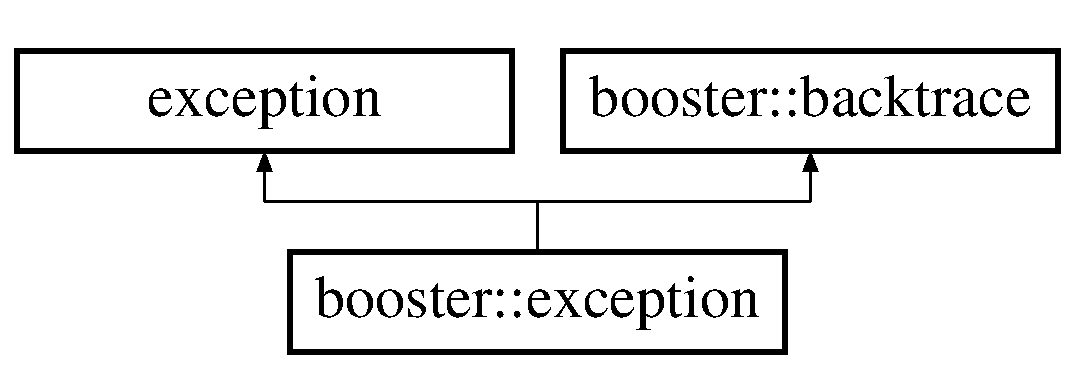
\includegraphics[height=2.000000cm]{classbooster_1_1exception}
\end{center}
\end{figure}
\subsection*{Additional Inherited Members}


\subsection{Detailed Description}
Same as std\+::exception but records stack trace. 

The documentation for this class was generated from the following file\+:\begin{DoxyCompactItemize}
\item 
booster/backtrace.\+h\end{DoxyCompactItemize}

\section{cppcms\+:\+:applications\+\_\+pool\+:\+:factory Struct Reference}
\label{structcppcms_1_1applications__pool_1_1factory}\index{cppcms\+::applications\+\_\+pool\+::factory@{cppcms\+::applications\+\_\+pool\+::factory}}


a base class for user application factories -\/ to be deprecated, use \doxyref{application\+\_\+specific\+\_\+pool}{p.}{classcppcms_1_1application__specific__pool} instead  




{\ttfamily \#include $<$cppcms/applications\+\_\+pool.\+h$>$}

Inheritance diagram for cppcms\+:\+:applications\+\_\+pool\+:\+:factory\+:\begin{figure}[H]
\begin{center}
\leavevmode
\includegraphics[height=2.000000cm]{structcppcms_1_1applications__pool_1_1factory}
\end{center}
\end{figure}
\subsection*{Public Member Functions}
\begin{DoxyCompactItemize}
\item 
virtual std\+::unique\+\_\+ptr$<$ {\bf application} $>$ {\bf operator()} ({\bf service} \&) const =0
\end{DoxyCompactItemize}


\subsection{Detailed Description}
a base class for user application factories -\/ to be deprecated, use \doxyref{application\+\_\+specific\+\_\+pool}{p.}{classcppcms_1_1application__specific__pool} instead 

\begin{DoxyRefDesc}{Deprecated}
\item[{\bf Deprecated}]Use \doxyref{application\+\_\+specific\+\_\+pool}{p.}{classcppcms_1_1application__specific__pool} \end{DoxyRefDesc}


\subsection{Member Function Documentation}
\index{cppcms\+::applications\+\_\+pool\+::factory@{cppcms\+::applications\+\_\+pool\+::factory}!operator()@{operator()}}
\index{operator()@{operator()}!cppcms\+::applications\+\_\+pool\+::factory@{cppcms\+::applications\+\_\+pool\+::factory}}
\subsubsection[{operator()(service \&) const =0}]{\setlength{\rightskip}{0pt plus 5cm}virtual std\+::unique\+\_\+ptr$<${\bf application}$>$ cppcms\+::applications\+\_\+pool\+::factory\+::operator() (
\begin{DoxyParamCaption}
\item[{{\bf service} \&}]{}
\end{DoxyParamCaption}
) const\hspace{0.3cm}{\ttfamily [pure virtual]}}\label{structcppcms_1_1applications__pool_1_1factory_acdbd3411dd725e89c6bf7e5fc96166bd}
Returns newly created instance of an application. 

The documentation for this struct was generated from the following file\+:\begin{DoxyCompactItemize}
\item 
cppcms/applications\+\_\+pool.\+h\end{DoxyCompactItemize}

\section{cppcms\+:\+:http\+:\+:file Class Reference}
\label{classcppcms_1_1http_1_1file}\index{cppcms\+::http\+::file@{cppcms\+::http\+::file}}


This class holds a uploaded file, it is generally fetched via \doxyref{widgets\+::file}{p.}{classcppcms_1_1widgets_1_1file} or via {\tt http\+::request\+::files}.  




{\ttfamily \#include $<$cppcms/http\+\_\+file.\+h$>$}

Inheritance diagram for cppcms\+:\+:http\+:\+:file\+:\begin{figure}[H]
\begin{center}
\leavevmode
\includegraphics[height=2.000000cm]{classcppcms_1_1http_1_1file}
\end{center}
\end{figure}
\subsection*{Public Member Functions}
\begin{DoxyCompactItemize}
\item 
std\+::string {\bf name} () const 
\item 
std\+::string {\bf mime} () const 
\item 
bool {\bf has\+\_\+mime} () const 
\item 
std\+::string {\bf filename} () const 
\item 
std\+::istream \& {\bf data} ()
\item 
long long {\bf size} ()
\item 
void {\bf output\+\_\+file} (std\+::string const \&{\bf name}, bool is\+\_\+temporary=false)
\item 
void {\bf make\+\_\+permanent} ()
\item 
int {\bf close} ()
\item 
void {\bf save\+\_\+to} (std\+::string const \&{\bf filename})
\item 
void {\bf set\+\_\+memory\+\_\+limit} (size\+\_\+t {\bf size})
\item 
void {\bf set\+\_\+temporary\+\_\+directory} (std\+::string const \&dir)
\end{DoxyCompactItemize}
\subsection*{Friends}
\begin{DoxyCompactItemize}
\item 
class {\bfseries request}\label{classcppcms_1_1http_1_1file_a85b2d00ed5d8672f7dbb26f19a0b6123}

\end{DoxyCompactItemize}


\subsection{Detailed Description}
This class holds a uploaded file, it is generally fetched via \doxyref{widgets\+::file}{p.}{classcppcms_1_1widgets_1_1file} or via {\tt http\+::request\+::files}. 

It provides full information about uploaded data as it was send by browser and allows to read the file via std\+::istream seek-\/able interface or save to the file system

Note\+: this class does not perform any validations, for checking the data use \doxyref{widgets\+::file}{p.}{classcppcms_1_1widgets_1_1file} that allows to perform numerous checks on the file data. 

\subsection{Member Function Documentation}
\index{cppcms\+::http\+::file@{cppcms\+::http\+::file}!close@{close}}
\index{close@{close}!cppcms\+::http\+::file@{cppcms\+::http\+::file}}
\subsubsection[{close()}]{\setlength{\rightskip}{0pt plus 5cm}int cppcms\+::http\+::file\+::close (
\begin{DoxyParamCaption}
{}
\end{DoxyParamCaption}
)}\label{classcppcms_1_1http_1_1file_a81bff76b6569f661b18f07dae57025c7}
Close the file if it is still open, if the file temporary it is deleted, the the file in memory its content is removed, \doxyref{data()}{p.}{classcppcms_1_1http_1_1file_a3a95bc7fefe80a75bc098baa3ad8c400} would return non-\/usable stream

Returns 0 in case of sucess and -\/1 in case of failure

\doxyref{New in Cpp\+C\+MS 1.\+2}{p.}{v1_2} \index{cppcms\+::http\+::file@{cppcms\+::http\+::file}!data@{data}}
\index{data@{data}!cppcms\+::http\+::file@{cppcms\+::http\+::file}}
\subsubsection[{data()}]{\setlength{\rightskip}{0pt plus 5cm}std\+::istream\& cppcms\+::http\+::file\+::data (
\begin{DoxyParamCaption}
{}
\end{DoxyParamCaption}
)}\label{classcppcms_1_1http_1_1file_a3a95bc7fefe80a75bc098baa3ad8c400}
Get std\+::istream on the data, please note, you need to call \doxyref{data()}{p.}{classcppcms_1_1http_1_1file_a3a95bc7fefe80a75bc098baa3ad8c400}.seekg(0) when using this stream first time. \index{cppcms\+::http\+::file@{cppcms\+::http\+::file}!filename@{filename}}
\index{filename@{filename}!cppcms\+::http\+::file@{cppcms\+::http\+::file}}
\subsubsection[{filename() const }]{\setlength{\rightskip}{0pt plus 5cm}std\+::string cppcms\+::http\+::file\+::filename (
\begin{DoxyParamCaption}
{}
\end{DoxyParamCaption}
) const}\label{classcppcms_1_1http_1_1file_aec7aaa5ab4f57aada988507d5d299f6f}
Get the filename as it was sent by the browser. \index{cppcms\+::http\+::file@{cppcms\+::http\+::file}!has\+\_\+mime@{has\+\_\+mime}}
\index{has\+\_\+mime@{has\+\_\+mime}!cppcms\+::http\+::file@{cppcms\+::http\+::file}}
\subsubsection[{has\+\_\+mime() const }]{\setlength{\rightskip}{0pt plus 5cm}bool cppcms\+::http\+::file\+::has\+\_\+mime (
\begin{DoxyParamCaption}
{}
\end{DoxyParamCaption}
) const}\label{classcppcms_1_1http_1_1file_a6f94cc6fc4068828a74fe8110cc295b1}
Returns true if content type defined

\doxyref{New in Cpp\+C\+MS 1.\+2}{p.}{v1_2} \index{cppcms\+::http\+::file@{cppcms\+::http\+::file}!make\+\_\+permanent@{make\+\_\+permanent}}
\index{make\+\_\+permanent@{make\+\_\+permanent}!cppcms\+::http\+::file@{cppcms\+::http\+::file}}
\subsubsection[{make\+\_\+permanent()}]{\setlength{\rightskip}{0pt plus 5cm}void cppcms\+::http\+::file\+::make\+\_\+permanent (
\begin{DoxyParamCaption}
{}
\end{DoxyParamCaption}
)}\label{classcppcms_1_1http_1_1file_a10a75d543175cd0a69bbbc44049efc26}
Make sure that file created by output\+\_\+file member function is not removed in destructor

\doxyref{New in Cpp\+C\+MS 1.\+2}{p.}{v1_2} \index{cppcms\+::http\+::file@{cppcms\+::http\+::file}!mime@{mime}}
\index{mime@{mime}!cppcms\+::http\+::file@{cppcms\+::http\+::file}}
\subsubsection[{mime() const }]{\setlength{\rightskip}{0pt plus 5cm}std\+::string cppcms\+::http\+::file\+::mime (
\begin{DoxyParamCaption}
{}
\end{DoxyParamCaption}
) const}\label{classcppcms_1_1http_1_1file_ab8d8de07a1bf0ce904737dfe53a017bd}
Get the content-\/type of the file as it was sent by the browser. \index{cppcms\+::http\+::file@{cppcms\+::http\+::file}!name@{name}}
\index{name@{name}!cppcms\+::http\+::file@{cppcms\+::http\+::file}}
\subsubsection[{name() const }]{\setlength{\rightskip}{0pt plus 5cm}std\+::string cppcms\+::http\+::file\+::name (
\begin{DoxyParamCaption}
{}
\end{DoxyParamCaption}
) const}\label{classcppcms_1_1http_1_1file_ab2691618c7312d598a080d60410bad00}
Get the name of the P\+O\+ST field (i.\+e. $<$input name=\char`\"{}value\char`\"{} ...$>$) \index{cppcms\+::http\+::file@{cppcms\+::http\+::file}!output\+\_\+file@{output\+\_\+file}}
\index{output\+\_\+file@{output\+\_\+file}!cppcms\+::http\+::file@{cppcms\+::http\+::file}}
\subsubsection[{output\+\_\+file(std\+::string const \&name, bool is\+\_\+temporary=false)}]{\setlength{\rightskip}{0pt plus 5cm}void cppcms\+::http\+::file\+::output\+\_\+file (
\begin{DoxyParamCaption}
\item[{std\+::string const \&}]{name, }
\item[{bool}]{is\+\_\+temporary = {\ttfamily false}}
\end{DoxyParamCaption}
)}\label{classcppcms_1_1http_1_1file_a9fcb51feca28d1ad113552f63ab82896}
Specify the path to the output file, note if is\+\_\+temporary is true than the file would be deleted on \doxyref{cppcms\+::http\+::file}{p.}{classcppcms_1_1http_1_1file} destruction, unless save\+\_\+to is called, otherwise it would remain persistent

\doxyref{New in Cpp\+C\+MS 1.\+2}{p.}{v1_2} \index{cppcms\+::http\+::file@{cppcms\+::http\+::file}!save\+\_\+to@{save\+\_\+to}}
\index{save\+\_\+to@{save\+\_\+to}!cppcms\+::http\+::file@{cppcms\+::http\+::file}}
\subsubsection[{save\+\_\+to(std\+::string const \&filename)}]{\setlength{\rightskip}{0pt plus 5cm}void cppcms\+::http\+::file\+::save\+\_\+to (
\begin{DoxyParamCaption}
\item[{std\+::string const \&}]{filename}
\end{DoxyParamCaption}
)}\label{classcppcms_1_1http_1_1file_a981a2325266c685788f8e241f2154308}
Save file to file named {\itshape filename}. Throws \doxyref{cppcms\+\_\+error}{p.}{classcppcms_1_1cppcms__error} in case of failure.

Notes\+:


\begin{DoxyItemize}
\item this function maybe more efficient then just reading the stream and writing it to newly created file, as in case of big files, it would try to move it over the file system
\item Under Win32 {\itshape filename} should be U\+T\+F-\/8 string 
\end{DoxyItemize}\index{cppcms\+::http\+::file@{cppcms\+::http\+::file}!set\+\_\+memory\+\_\+limit@{set\+\_\+memory\+\_\+limit}}
\index{set\+\_\+memory\+\_\+limit@{set\+\_\+memory\+\_\+limit}!cppcms\+::http\+::file@{cppcms\+::http\+::file}}
\subsubsection[{set\+\_\+memory\+\_\+limit(size\+\_\+t size)}]{\setlength{\rightskip}{0pt plus 5cm}void cppcms\+::http\+::file\+::set\+\_\+memory\+\_\+limit (
\begin{DoxyParamCaption}
\item[{size\+\_\+t}]{size}
\end{DoxyParamCaption}
)}\label{classcppcms_1_1http_1_1file_a11196e4f597b326da3623d78316e4bb9}
Set the maximal size of file that would be stored in memory instead of file system

\doxyref{New in Cpp\+C\+MS 1.\+2}{p.}{v1_2} \index{cppcms\+::http\+::file@{cppcms\+::http\+::file}!set\+\_\+temporary\+\_\+directory@{set\+\_\+temporary\+\_\+directory}}
\index{set\+\_\+temporary\+\_\+directory@{set\+\_\+temporary\+\_\+directory}!cppcms\+::http\+::file@{cppcms\+::http\+::file}}
\subsubsection[{set\+\_\+temporary\+\_\+directory(std\+::string const \&dir)}]{\setlength{\rightskip}{0pt plus 5cm}void cppcms\+::http\+::file\+::set\+\_\+temporary\+\_\+directory (
\begin{DoxyParamCaption}
\item[{std\+::string const \&}]{dir}
\end{DoxyParamCaption}
)}\label{classcppcms_1_1http_1_1file_a0e3eb2d67f37ef413915d43f166ec6fe}
Set the temporary directory where uploaded files are created

\doxyref{New in Cpp\+C\+MS 1.\+2}{p.}{v1_2} \index{cppcms\+::http\+::file@{cppcms\+::http\+::file}!size@{size}}
\index{size@{size}!cppcms\+::http\+::file@{cppcms\+::http\+::file}}
\subsubsection[{size()}]{\setlength{\rightskip}{0pt plus 5cm}long long cppcms\+::http\+::file\+::size (
\begin{DoxyParamCaption}
{}
\end{DoxyParamCaption}
)}\label{classcppcms_1_1http_1_1file_aee3dac0ba0afc1128c0a20b72c998238}
Get the size of the file. 

The documentation for this class was generated from the following file\+:\begin{DoxyCompactItemize}
\item 
cppcms/http\+\_\+file.\+h\end{DoxyCompactItemize}

\section{booster\+:\+:log\+:\+:sinks\+:\+:file Class Reference}
\label{classbooster_1_1log_1_1sinks_1_1file}\index{booster\+::log\+::sinks\+::file@{booster\+::log\+::sinks\+::file}}


log file based sink -\/ sends messages to log file  




{\ttfamily \#include $<$booster/booster/log.\+h$>$}

Inheritance diagram for booster\+:\+:log\+:\+:sinks\+:\+:file\+:\begin{figure}[H]
\begin{center}
\leavevmode
\includegraphics[height=3.000000cm]{classbooster_1_1log_1_1sinks_1_1file}
\end{center}
\end{figure}
\subsection*{Public Member Functions}
\begin{DoxyCompactItemize}
\item 
{\bf file} ()
\item 
{\bf file} (std\+::string const \&file\+\_\+name, int {\bf max\+\_\+files}=0)
\item 
void {\bf open} (std\+::string file\+\_\+name)
\item 
void {\bf max\+\_\+files} (unsigned limit)
\item 
void {\bf append} ()
\item 
void {\bf set\+\_\+timezone} (std\+::string const \&name)
\item 
virtual void {\bf log} ({\bf message} const \&)\label{classbooster_1_1log_1_1sinks_1_1file_ad2a5335abaff993da082fb124056748a}

\begin{DoxyCompactList}\small\item\em Send message to the log. \end{DoxyCompactList}\end{DoxyCompactItemize}
\subsection*{Static Public Attributes}
\begin{DoxyCompactItemize}
\item 
static const int {\bf app} = -\/1
\end{DoxyCompactItemize}


\subsection{Detailed Description}
log file based sink -\/ sends messages to log file 

\subsection{Constructor \& Destructor Documentation}
\index{booster\+::log\+::sinks\+::file@{booster\+::log\+::sinks\+::file}!file@{file}}
\index{file@{file}!booster\+::log\+::sinks\+::file@{booster\+::log\+::sinks\+::file}}
\subsubsection[{file()}]{\setlength{\rightskip}{0pt plus 5cm}booster\+::log\+::sinks\+::file\+::file (
\begin{DoxyParamCaption}
{}
\end{DoxyParamCaption}
)}\label{classbooster_1_1log_1_1sinks_1_1file_aa4c6bd1485f996a68b138beb27901085}
Creates new object but does not open a file \index{booster\+::log\+::sinks\+::file@{booster\+::log\+::sinks\+::file}!file@{file}}
\index{file@{file}!booster\+::log\+::sinks\+::file@{booster\+::log\+::sinks\+::file}}
\subsubsection[{file(std\+::string const \&file\+\_\+name, int max\+\_\+files=0)}]{\setlength{\rightskip}{0pt plus 5cm}booster\+::log\+::sinks\+::file\+::file (
\begin{DoxyParamCaption}
\item[{std\+::string const \&}]{file\+\_\+name, }
\item[{int}]{max\+\_\+files = {\ttfamily 0}}
\end{DoxyParamCaption}
)}\label{classbooster_1_1log_1_1sinks_1_1file_a95522ba36423329564f466ff56854aaf}
Creates new file sink named {\itshape file\+\_\+name}, if max\+\_\+files = app, then no new files created but rather the log is appended to the existing file

\doxyref{New in Cpp\+C\+MS 1.\+2}{p.}{v1_2} 

\subsection{Member Function Documentation}
\index{booster\+::log\+::sinks\+::file@{booster\+::log\+::sinks\+::file}!append@{append}}
\index{append@{append}!booster\+::log\+::sinks\+::file@{booster\+::log\+::sinks\+::file}}
\subsubsection[{append()}]{\setlength{\rightskip}{0pt plus 5cm}void booster\+::log\+::sinks\+::file\+::append (
\begin{DoxyParamCaption}
{}
\end{DoxyParamCaption}
)}\label{classbooster_1_1log_1_1sinks_1_1file_a0fd3a432eca836a03116ca4d987aa3fc}
Append to output file rather then create new one. \index{booster\+::log\+::sinks\+::file@{booster\+::log\+::sinks\+::file}!max\+\_\+files@{max\+\_\+files}}
\index{max\+\_\+files@{max\+\_\+files}!booster\+::log\+::sinks\+::file@{booster\+::log\+::sinks\+::file}}
\subsubsection[{max\+\_\+files(unsigned limit)}]{\setlength{\rightskip}{0pt plus 5cm}void booster\+::log\+::sinks\+::file\+::max\+\_\+files (
\begin{DoxyParamCaption}
\item[{unsigned}]{limit}
\end{DoxyParamCaption}
)}\label{classbooster_1_1log_1_1sinks_1_1file_a6c1bc0a6f42b13432fcde198b5988124}
Enable file rotation and set the maximal number of files that should be kept.

Each time the log opened, the old files are renamed, if there are more files then {\itshape limit}, the oldest is removed \index{booster\+::log\+::sinks\+::file@{booster\+::log\+::sinks\+::file}!open@{open}}
\index{open@{open}!booster\+::log\+::sinks\+::file@{booster\+::log\+::sinks\+::file}}
\subsubsection[{open(std\+::string file\+\_\+name)}]{\setlength{\rightskip}{0pt plus 5cm}void booster\+::log\+::sinks\+::file\+::open (
\begin{DoxyParamCaption}
\item[{std\+::string}]{file\+\_\+name}
\end{DoxyParamCaption}
)}\label{classbooster_1_1log_1_1sinks_1_1file_ae4569b5691c3ce315a35c40239cc6def}
Open log file \index{booster\+::log\+::sinks\+::file@{booster\+::log\+::sinks\+::file}!set\+\_\+timezone@{set\+\_\+timezone}}
\index{set\+\_\+timezone@{set\+\_\+timezone}!booster\+::log\+::sinks\+::file@{booster\+::log\+::sinks\+::file}}
\subsubsection[{set\+\_\+timezone(std\+::string const \&name)}]{\setlength{\rightskip}{0pt plus 5cm}void booster\+::log\+::sinks\+::file\+::set\+\_\+timezone (
\begin{DoxyParamCaption}
\item[{std\+::string const \&}]{name}
\end{DoxyParamCaption}
)}\label{classbooster_1_1log_1_1sinks_1_1file_ab6b94e47185d583d40da2cc8f8faadfa}
Set the time-\/zone name that should be used in the message.

It should have a format G\+M\+T+\+XX\+:YY like \char`\"{}\+G\+M\+T+2\+:00\char`\"{} or \char`\"{}\+G\+M\+T-\/3\char`\"{}. \char`\"{}\+G\+M\+T\char`\"{} can be used as well

If name is empty local time is used which is the default 

\subsection{Member Data Documentation}
\index{booster\+::log\+::sinks\+::file@{booster\+::log\+::sinks\+::file}!app@{app}}
\index{app@{app}!booster\+::log\+::sinks\+::file@{booster\+::log\+::sinks\+::file}}
\subsubsection[{app}]{\setlength{\rightskip}{0pt plus 5cm}const int booster\+::log\+::sinks\+::file\+::app = -\/1\hspace{0.3cm}{\ttfamily [static]}}\label{classbooster_1_1log_1_1sinks_1_1file_a436b83f0460e92b59300b84f19c1ca1e}
Flag that can be passed to constructor that specifies that the log should be appended to the existing file

\doxyref{New in Cpp\+C\+MS 1.\+2}{p.}{v1_2} 

The documentation for this class was generated from the following file\+:\begin{DoxyCompactItemize}
\item 
booster/{\bf log.\+h}\end{DoxyCompactItemize}

\section{cppcms\+:\+:widgets\+:\+:file Class Reference}
\label{classcppcms_1_1widgets_1_1file}\index{cppcms\+::widgets\+::file@{cppcms\+::widgets\+::file}}


This class represents a file upload form entry.  




{\ttfamily \#include $<$cppcms/form.\+h$>$}

Inheritance diagram for cppcms\+:\+:widgets\+:\+:file\+:\begin{figure}[H]
\begin{center}
\leavevmode
\includegraphics[height=5.000000cm]{classcppcms_1_1widgets_1_1file}
\end{center}
\end{figure}
\subsection*{Public Member Functions}
\begin{DoxyCompactItemize}
\item 
void {\bf non\+\_\+empty} ()
\item 
void {\bf limits} (int min, int max)
\item 
std\+::pair$<$ int, int $>$ {\bf limits} ()
\item 
void {\bf filename} ({\bf booster\+::regex} const \&fn)
\item 
{\bf booster\+::regex} {\bf filename} ()
\item 
void {\bf validate\+\_\+filename\+\_\+charset} (bool)
\item 
bool {\bf validate\+\_\+filename\+\_\+charset} ()
\item 
booster\+::shared\+\_\+ptr$<$ {\bf http\+::file} $>$ {\bf value} ()
\item 
void {\bf mime} (std\+::string const \&)
\item 
void {\bf mime} ({\bf booster\+::regex} const \&expr)
\item 
void {\bf add\+\_\+valid\+\_\+magic} (std\+::string const \&)
\item 
virtual void {\bf load} ({\bf http\+::context} \&context)
\item 
virtual void {\bf render\+\_\+value} ({\bf form\+\_\+context} \&context)
\item 
virtual bool {\bf validate} ()
\end{DoxyCompactItemize}
\subsection*{Additional Inherited Members}


\subsection{Detailed Description}
This class represents a file upload form entry. 

If the file was not uploaded, \doxyref{set()}{p.}{classcppcms_1_1widgets_1_1base__widget_afd814f0d448866c0f316e38e05fc8d3f} will be false and an attempt to access the member function \doxyref{value()}{p.}{classcppcms_1_1widgets_1_1file_a56ee053415b1bd98944bb3599e3392b1} will throw. 

\subsection{Member Function Documentation}
\index{cppcms\+::widgets\+::file@{cppcms\+::widgets\+::file}!add\+\_\+valid\+\_\+magic@{add\+\_\+valid\+\_\+magic}}
\index{add\+\_\+valid\+\_\+magic@{add\+\_\+valid\+\_\+magic}!cppcms\+::widgets\+::file@{cppcms\+::widgets\+::file}}
\subsubsection[{add\+\_\+valid\+\_\+magic(std\+::string const \&)}]{\setlength{\rightskip}{0pt plus 5cm}void cppcms\+::widgets\+::file\+::add\+\_\+valid\+\_\+magic (
\begin{DoxyParamCaption}
\item[{std\+::string const \&}]{}
\end{DoxyParamCaption}
)}\label{classcppcms_1_1widgets_1_1file_a1d53934bdd93266e3bfbec26a8afe09e}
Add a string that represents a valid magic number that shoud exist on begging of file.

By default no tests are performed. \index{cppcms\+::widgets\+::file@{cppcms\+::widgets\+::file}!filename@{filename}}
\index{filename@{filename}!cppcms\+::widgets\+::file@{cppcms\+::widgets\+::file}}
\subsubsection[{filename(booster\+::regex const \&fn)}]{\setlength{\rightskip}{0pt plus 5cm}void cppcms\+::widgets\+::file\+::filename (
\begin{DoxyParamCaption}
\item[{{\bf booster\+::regex} const \&}]{fn}
\end{DoxyParamCaption}
)}\label{classcppcms_1_1widgets_1_1file_a4b60527ec447de253d8f8dbb728869cb}
Set the filename validation pattern. For example \char`\"{}.$\ast$\textbackslash{}\textbackslash{}.(jpg$\vert$jpeg$\vert$png)\char`\"{}.

Please, note that it is a good idea to check magic numbers as well and not rely on file name only.

See \doxyref{add\+\_\+valid\+\_\+magic()}{p.}{classcppcms_1_1widgets_1_1file_a1d53934bdd93266e3bfbec26a8afe09e} function \index{cppcms\+::widgets\+::file@{cppcms\+::widgets\+::file}!filename@{filename}}
\index{filename@{filename}!cppcms\+::widgets\+::file@{cppcms\+::widgets\+::file}}
\subsubsection[{filename()}]{\setlength{\rightskip}{0pt plus 5cm}{\bf booster\+::regex} cppcms\+::widgets\+::file\+::filename (
\begin{DoxyParamCaption}
{}
\end{DoxyParamCaption}
)}\label{classcppcms_1_1widgets_1_1file_ad5e888416710dfd7b3ba9c0651b4b476}
Get the regular expression for the filename validation. \index{cppcms\+::widgets\+::file@{cppcms\+::widgets\+::file}!limits@{limits}}
\index{limits@{limits}!cppcms\+::widgets\+::file@{cppcms\+::widgets\+::file}}
\subsubsection[{limits(int min, int max)}]{\setlength{\rightskip}{0pt plus 5cm}void cppcms\+::widgets\+::file\+::limits (
\begin{DoxyParamCaption}
\item[{int}]{min, }
\item[{int}]{max}
\end{DoxyParamCaption}
)}\label{classcppcms_1_1widgets_1_1file_a348f7619cd476672c8018e6a8c9e2ed1}
Set the minimum and maximum limits for the file size. Note\+: max == -\/1 indicates that there is no maximum limit; min==0 indicates that there is no minimum limit. \index{cppcms\+::widgets\+::file@{cppcms\+::widgets\+::file}!limits@{limits}}
\index{limits@{limits}!cppcms\+::widgets\+::file@{cppcms\+::widgets\+::file}}
\subsubsection[{limits()}]{\setlength{\rightskip}{0pt plus 5cm}std\+::pair$<$int,int$>$ cppcms\+::widgets\+::file\+::limits (
\begin{DoxyParamCaption}
{}
\end{DoxyParamCaption}
)}\label{classcppcms_1_1widgets_1_1file_aba42fd04191fbd11e148907f0441b649}
Get the minimum and maximum size limits. \index{cppcms\+::widgets\+::file@{cppcms\+::widgets\+::file}!load@{load}}
\index{load@{load}!cppcms\+::widgets\+::file@{cppcms\+::widgets\+::file}}
\subsubsection[{load(http\+::context \&context)}]{\setlength{\rightskip}{0pt plus 5cm}virtual void cppcms\+::widgets\+::file\+::load (
\begin{DoxyParamCaption}
\item[{{\bf http\+::context} \&}]{context}
\end{DoxyParamCaption}
)\hspace{0.3cm}{\ttfamily [virtual]}}\label{classcppcms_1_1widgets_1_1file_acd5589f0f6a99c6f5590ee2787d407d7}
Load the form information from the provided {\tt http\+::context} {\itshape context}. A user can call this function to load all information from the raw P\+O\+S\+T/\+G\+ET data into the internal widget representation. 

Implements {\bf cppcms\+::base\+\_\+form} \doxyref{}{p.}{classcppcms_1_1base__form_a5f9c5bbfba18076e898ec95827656bc1}.

\index{cppcms\+::widgets\+::file@{cppcms\+::widgets\+::file}!mime@{mime}}
\index{mime@{mime}!cppcms\+::widgets\+::file@{cppcms\+::widgets\+::file}}
\subsubsection[{mime(std\+::string const \&)}]{\setlength{\rightskip}{0pt plus 5cm}void cppcms\+::widgets\+::file\+::mime (
\begin{DoxyParamCaption}
\item[{std\+::string const \&}]{}
\end{DoxyParamCaption}
)}\label{classcppcms_1_1widgets_1_1file_a5acb1facf885ee351e0fd0ffb2900e0d}
Set the required file mime type. \index{cppcms\+::widgets\+::file@{cppcms\+::widgets\+::file}!mime@{mime}}
\index{mime@{mime}!cppcms\+::widgets\+::file@{cppcms\+::widgets\+::file}}
\subsubsection[{mime(booster\+::regex const \&expr)}]{\setlength{\rightskip}{0pt plus 5cm}void cppcms\+::widgets\+::file\+::mime (
\begin{DoxyParamCaption}
\item[{{\bf booster\+::regex} const \&}]{expr}
\end{DoxyParamCaption}
)}\label{classcppcms_1_1widgets_1_1file_a39eebaccd0036cd0568e8f61b9787c0f}
Set the regular expression to validate the mime type. \index{cppcms\+::widgets\+::file@{cppcms\+::widgets\+::file}!non\+\_\+empty@{non\+\_\+empty}}
\index{non\+\_\+empty@{non\+\_\+empty}!cppcms\+::widgets\+::file@{cppcms\+::widgets\+::file}}
\subsubsection[{non\+\_\+empty()}]{\setlength{\rightskip}{0pt plus 5cm}void cppcms\+::widgets\+::file\+::non\+\_\+empty (
\begin{DoxyParamCaption}
{}
\end{DoxyParamCaption}
)}\label{classcppcms_1_1widgets_1_1file_aa85b2dd9f67c7042b87c7c917a3a3c47}
Ensure that a file is uploaded (for the validation). \index{cppcms\+::widgets\+::file@{cppcms\+::widgets\+::file}!render\+\_\+value@{render\+\_\+value}}
\index{render\+\_\+value@{render\+\_\+value}!cppcms\+::widgets\+::file@{cppcms\+::widgets\+::file}}
\subsubsection[{render\+\_\+value(form\+\_\+context \&context)}]{\setlength{\rightskip}{0pt plus 5cm}virtual void cppcms\+::widgets\+::file\+::render\+\_\+value (
\begin{DoxyParamCaption}
\item[{{\bf form\+\_\+context} \&}]{context}
\end{DoxyParamCaption}
)\hspace{0.3cm}{\ttfamily [virtual]}}\label{classcppcms_1_1widgets_1_1file_aa607511349c879b6e0c1a395f270f76d}
Write the actual value of the H\+T\+ML tag. Derived classes must implement this. 

Implements {\bf cppcms\+::widgets\+::base\+\_\+html\+\_\+input} \doxyref{}{p.}{classcppcms_1_1widgets_1_1base__html__input_afd2f99f7dd7b8ebe75e63f1f005068cb}.

\index{cppcms\+::widgets\+::file@{cppcms\+::widgets\+::file}!validate@{validate}}
\index{validate@{validate}!cppcms\+::widgets\+::file@{cppcms\+::widgets\+::file}}
\subsubsection[{validate()}]{\setlength{\rightskip}{0pt plus 5cm}virtual bool cppcms\+::widgets\+::file\+::validate (
\begin{DoxyParamCaption}
{}
\end{DoxyParamCaption}
)\hspace{0.3cm}{\ttfamily [virtual]}}\label{classcppcms_1_1widgets_1_1file_addfa723594f3658578787843fa030486}
Validate the form. If not overridden, it sets the widget to {\itshape valid}. 

Reimplemented from {\bf cppcms\+::widgets\+::base\+\_\+widget} \doxyref{}{p.}{classcppcms_1_1widgets_1_1base__widget_a090169cd0b61fdaceac8ed1b0ca47749}.

\index{cppcms\+::widgets\+::file@{cppcms\+::widgets\+::file}!validate\+\_\+filename\+\_\+charset@{validate\+\_\+filename\+\_\+charset}}
\index{validate\+\_\+filename\+\_\+charset@{validate\+\_\+filename\+\_\+charset}!cppcms\+::widgets\+::file@{cppcms\+::widgets\+::file}}
\subsubsection[{validate\+\_\+filename\+\_\+charset(bool)}]{\setlength{\rightskip}{0pt plus 5cm}void cppcms\+::widgets\+::file\+::validate\+\_\+filename\+\_\+charset (
\begin{DoxyParamCaption}
\item[{bool}]{}
\end{DoxyParamCaption}
)}\label{classcppcms_1_1widgets_1_1file_a7993906a8b128c903ad44f9f4101848d}
Validate or not the filename\textquotesingle{}s charset. The default is {\itshape true}. \index{cppcms\+::widgets\+::file@{cppcms\+::widgets\+::file}!validate\+\_\+filename\+\_\+charset@{validate\+\_\+filename\+\_\+charset}}
\index{validate\+\_\+filename\+\_\+charset@{validate\+\_\+filename\+\_\+charset}!cppcms\+::widgets\+::file@{cppcms\+::widgets\+::file}}
\subsubsection[{validate\+\_\+filename\+\_\+charset()}]{\setlength{\rightskip}{0pt plus 5cm}bool cppcms\+::widgets\+::file\+::validate\+\_\+filename\+\_\+charset (
\begin{DoxyParamCaption}
{}
\end{DoxyParamCaption}
)}\label{classcppcms_1_1widgets_1_1file_a12727b17d2e869ad7634442b9de5a9c2}
Get the validation option for the filename\textquotesingle{}s charset. \index{cppcms\+::widgets\+::file@{cppcms\+::widgets\+::file}!value@{value}}
\index{value@{value}!cppcms\+::widgets\+::file@{cppcms\+::widgets\+::file}}
\subsubsection[{value()}]{\setlength{\rightskip}{0pt plus 5cm}booster\+::shared\+\_\+ptr$<${\bf http\+::file}$>$ cppcms\+::widgets\+::file\+::value (
\begin{DoxyParamCaption}
{}
\end{DoxyParamCaption}
)}\label{classcppcms_1_1widgets_1_1file_a56ee053415b1bd98944bb3599e3392b1}
Get the uploaded file. This throws \doxyref{cppcms\+\_\+error}{p.}{classcppcms_1_1cppcms__error} if \doxyref{set()}{p.}{classcppcms_1_1widgets_1_1base__widget_afd814f0d448866c0f316e38e05fc8d3f} == false, i.\+e. if no file was uploaded. 

The documentation for this class was generated from the following file\+:\begin{DoxyCompactItemize}
\item 
cppcms/form.\+h\end{DoxyCompactItemize}

\section{cppcms\+:\+:util\+:\+:filterbuf$<$ Filter, Buffer\+Size $>$ Class Template Reference}
\label{classcppcms_1_1util_1_1filterbuf}\index{cppcms\+::util\+::filterbuf$<$ Filter, Buffer\+Size $>$@{cppcms\+::util\+::filterbuf$<$ Filter, Buffer\+Size $>$}}
Inheritance diagram for cppcms\+:\+:util\+:\+:filterbuf$<$ Filter, Buffer\+Size $>$\+:\begin{figure}[H]
\begin{center}
\leavevmode
\includegraphics[height=2.000000cm]{classcppcms_1_1util_1_1filterbuf}
\end{center}
\end{figure}
\subsection*{Public Member Functions}
\begin{DoxyCompactItemize}
\item 
{\bfseries filterbuf} (std\+::ostream \&out)\label{classcppcms_1_1util_1_1filterbuf_ada8198a7f37907e26dbfb6d899cf5e79}

\item 
void {\bfseries steal} (std\+::ostream \&out)\label{classcppcms_1_1util_1_1filterbuf_aed458d9c98e96c6a7e1999c6b76e84e5}

\item 
int {\bfseries release} ()\label{classcppcms_1_1util_1_1filterbuf_a2185cd8578646eba289b6e6e7c2307a1}

\end{DoxyCompactItemize}
\subsection*{Protected Member Functions}
\begin{DoxyCompactItemize}
\item 
int {\bfseries overflow} (int c)\label{classcppcms_1_1util_1_1filterbuf_ab69ae3aee7bb1a420317c9971f73ddbd}

\end{DoxyCompactItemize}


The documentation for this class was generated from the following file\+:\begin{DoxyCompactItemize}
\item 
cppcms/steal\+\_\+buf.\+h\end{DoxyCompactItemize}

\section{cppcms\+:\+:util\+:\+:filterbuf$<$ Filter, 0 $>$ Class Template Reference}
\label{classcppcms_1_1util_1_1filterbuf_3_01Filter_00_010_01_4}\index{cppcms\+::util\+::filterbuf$<$ Filter, 0 $>$@{cppcms\+::util\+::filterbuf$<$ Filter, 0 $>$}}
Inheritance diagram for cppcms\+:\+:util\+:\+:filterbuf$<$ Filter, 0 $>$\+:\begin{figure}[H]
\begin{center}
\leavevmode
\includegraphics[height=2.000000cm]{classcppcms_1_1util_1_1filterbuf_3_01Filter_00_010_01_4}
\end{center}
\end{figure}
\subsection*{Public Member Functions}
\begin{DoxyCompactItemize}
\item 
{\bfseries filterbuf} (std\+::ostream \&out)\label{classcppcms_1_1util_1_1filterbuf_3_01Filter_00_010_01_4_a9849d6a053c34fd1a3563b6bc14eb5fc}

\item 
void {\bfseries steal} (std\+::ostream \&out)\label{classcppcms_1_1util_1_1filterbuf_3_01Filter_00_010_01_4_aa896287263e89b3df98261710adcc46a}

\item 
int {\bfseries release} ()\label{classcppcms_1_1util_1_1filterbuf_3_01Filter_00_010_01_4_a5d34d38c71a043c80f4f86725280c530}

\end{DoxyCompactItemize}
\subsection*{Protected Member Functions}
\begin{DoxyCompactItemize}
\item 
int {\bfseries overflow} (int c)\label{classcppcms_1_1util_1_1filterbuf_3_01Filter_00_010_01_4_a0a43979f703067b82b673def30704840}

\item 
std\+::streamsize {\bfseries xsputn} (char const $\ast$s, std\+::streamsize size)\label{classcppcms_1_1util_1_1filterbuf_3_01Filter_00_010_01_4_af82e5dd40084f73e9b8229590531da9f}

\end{DoxyCompactItemize}


The documentation for this class was generated from the following file\+:\begin{DoxyCompactItemize}
\item 
cppcms/steal\+\_\+buf.\+h\end{DoxyCompactItemize}

\section{cppcms\+:\+:form Class Reference}
\label{classcppcms_1_1form}\index{cppcms\+::form@{cppcms\+::form}}


The {\itshape form} is a container used to collect other widgets and forms into a single unit.  




{\ttfamily \#include $<$cppcms/form.\+h$>$}

Inheritance diagram for cppcms\+:\+:form\+:\begin{figure}[H]
\begin{center}
\leavevmode
\includegraphics[height=3.000000cm]{classcppcms_1_1form}
\end{center}
\end{figure}
\subsection*{Classes}
\begin{DoxyCompactItemize}
\item 
class {\bf iterator}
\begin{DoxyCompactList}\small\item\em Input iterator used to iterate over all the widgets in a form. \end{DoxyCompactList}\end{DoxyCompactItemize}
\subsection*{Public Member Functions}
\begin{DoxyCompactItemize}
\item 
virtual void {\bf render} ({\bf form\+\_\+context} \&context)
\item 
virtual void {\bf load} ({\bf http\+::context} \&cont)
\item 
virtual bool {\bf validate} ()
\item 
virtual void {\bf clear} ()
\item 
void {\bf add} ({\bf form} \&subform)
\item 
void {\bf attach} ({\bf form} $\ast$subform)
\item 
void {\bf add} ({\bf widgets\+::base\+\_\+widget} \&widget)
\item 
void {\bf attach} ({\bf widgets\+::base\+\_\+widget} $\ast$widget)
\item 
C\+P\+P\+C\+M\+S\+\_\+\+D\+E\+P\+R\+E\+C\+A\+T\+ED {\bf form} \& {\bf operator+} ({\bf form} \&f)
\item 
C\+P\+P\+C\+M\+S\+\_\+\+D\+E\+P\+R\+E\+C\+A\+T\+ED {\bf form} \& {\bf operator+} ({\bf widgets\+::base\+\_\+widget} \&f)
\item 
virtual void {\bf parent} ({\bf base\+\_\+form} $\ast$subform)
\item 
virtual {\bf form} $\ast$ {\bf parent} ()
\item 
{\bf iterator} {\bf begin} ()
\item 
{\bf iterator} {\bf end} ()
\end{DoxyCompactItemize}
\subsection*{Friends}
\begin{DoxyCompactItemize}
\item 
class {\bfseries iterator}\label{classcppcms_1_1form_a67171474c4da6cc8efe0c7fafefd2b2d}

\end{DoxyCompactItemize}
\subsection*{Additional Inherited Members}


\subsection{Detailed Description}
The {\itshape form} is a container used to collect other widgets and forms into a single unit. 

Generally various widgets and forms are combined into a single form in order to simplify their rendering and validation of the forms that include more than one widget. 

\subsection{Member Function Documentation}
\index{cppcms\+::form@{cppcms\+::form}!add@{add}}
\index{add@{add}!cppcms\+::form@{cppcms\+::form}}
\subsubsection[{add(form \&subform)}]{\setlength{\rightskip}{0pt plus 5cm}void cppcms\+::form\+::add (
\begin{DoxyParamCaption}
\item[{{\bf form} \&}]{subform}
\end{DoxyParamCaption}
)}\label{classcppcms_1_1form_a6b74acbbcb63dba5d1b4662ad9ee183c}
Add {\itshape subform} to form. The ownership is not transferred to the parent. \index{cppcms\+::form@{cppcms\+::form}!add@{add}}
\index{add@{add}!cppcms\+::form@{cppcms\+::form}}
\subsubsection[{add(widgets\+::base\+\_\+widget \&widget)}]{\setlength{\rightskip}{0pt plus 5cm}void cppcms\+::form\+::add (
\begin{DoxyParamCaption}
\item[{{\bf widgets\+::base\+\_\+widget} \&}]{widget}
\end{DoxyParamCaption}
)}\label{classcppcms_1_1form_a30ed5b2f98b0b6876639f7368d4673ce}
Add {\itshape widget} to form. The ownership is not transferred to to the parent. \index{cppcms\+::form@{cppcms\+::form}!attach@{attach}}
\index{attach@{attach}!cppcms\+::form@{cppcms\+::form}}
\subsubsection[{attach(form $\ast$subform)}]{\setlength{\rightskip}{0pt plus 5cm}void cppcms\+::form\+::attach (
\begin{DoxyParamCaption}
\item[{{\bf form} $\ast$}]{subform}
\end{DoxyParamCaption}
)}\label{classcppcms_1_1form_a774b66dee1c2b6b488d12243bc37a4b4}
Add {\itshape subform} to form. The ownership is transferred to the parent and the subform will be destroyed together with the parent. \index{cppcms\+::form@{cppcms\+::form}!attach@{attach}}
\index{attach@{attach}!cppcms\+::form@{cppcms\+::form}}
\subsubsection[{attach(widgets\+::base\+\_\+widget $\ast$widget)}]{\setlength{\rightskip}{0pt plus 5cm}void cppcms\+::form\+::attach (
\begin{DoxyParamCaption}
\item[{{\bf widgets\+::base\+\_\+widget} $\ast$}]{widget}
\end{DoxyParamCaption}
)}\label{classcppcms_1_1form_a8a21e075c3a19394a5680bfeb4b04ba9}
Add {\itshape widget} to form. The ownership is transferred to the parent and the widget will be destroyed together with the parent. \index{cppcms\+::form@{cppcms\+::form}!begin@{begin}}
\index{begin@{begin}!cppcms\+::form@{cppcms\+::form}}
\subsubsection[{begin()}]{\setlength{\rightskip}{0pt plus 5cm}{\bf iterator} cppcms\+::form\+::begin (
\begin{DoxyParamCaption}
{}
\end{DoxyParamCaption}
)}\label{classcppcms_1_1form_a64868bcf7a10d8c80f82e40afe7ae780}
Returns the iterator to the first widget. \index{cppcms\+::form@{cppcms\+::form}!clear@{clear}}
\index{clear@{clear}!cppcms\+::form@{cppcms\+::form}}
\subsubsection[{clear()}]{\setlength{\rightskip}{0pt plus 5cm}virtual void cppcms\+::form\+::clear (
\begin{DoxyParamCaption}
{}
\end{DoxyParamCaption}
)\hspace{0.3cm}{\ttfamily [virtual]}}\label{classcppcms_1_1form_a9c97ed57900d7404396135bbae33b809}
Clear all subforms and widgets from all loaded data. 

Implements {\bf cppcms\+::base\+\_\+form} \doxyref{}{p.}{classcppcms_1_1base__form_a69e995615d0cd577245480eb80ec834a}.

\index{cppcms\+::form@{cppcms\+::form}!end@{end}}
\index{end@{end}!cppcms\+::form@{cppcms\+::form}}
\subsubsection[{end()}]{\setlength{\rightskip}{0pt plus 5cm}{\bf iterator} cppcms\+::form\+::end (
\begin{DoxyParamCaption}
{}
\end{DoxyParamCaption}
)}\label{classcppcms_1_1form_ab267e93f7d7026742ebfb7b2047fb690}
Returns the end of the range iterator. \index{cppcms\+::form@{cppcms\+::form}!load@{load}}
\index{load@{load}!cppcms\+::form@{cppcms\+::form}}
\subsubsection[{load(http\+::context \&cont)}]{\setlength{\rightskip}{0pt plus 5cm}virtual void cppcms\+::form\+::load (
\begin{DoxyParamCaption}
\item[{{\bf http\+::context} \&}]{cont}
\end{DoxyParamCaption}
)\hspace{0.3cm}{\ttfamily [virtual]}}\label{classcppcms_1_1form_a56a59de72f0112b51f068f7511241912}
Load all the widget information from {\tt http\+::context} {\itshape cont}. 

Implements {\bf cppcms\+::base\+\_\+form} \doxyref{}{p.}{classcppcms_1_1base__form_a5f9c5bbfba18076e898ec95827656bc1}.

\index{cppcms\+::form@{cppcms\+::form}!operator+@{operator+}}
\index{operator+@{operator+}!cppcms\+::form@{cppcms\+::form}}
\subsubsection[{operator+(form \&f)}]{\setlength{\rightskip}{0pt plus 5cm}C\+P\+P\+C\+M\+S\+\_\+\+D\+E\+P\+R\+E\+C\+A\+T\+ED {\bf form}\& cppcms\+::form\+::operator+ (
\begin{DoxyParamCaption}
\item[{{\bf form} \&}]{f}
\end{DoxyParamCaption}
)\hspace{0.3cm}{\ttfamily [inline]}}\label{classcppcms_1_1form_aad7b901df499bc6d50eb8b156c6499a9}
\begin{DoxyRefDesc}{Deprecated}
\item[{\bf Deprecated}]Use \doxyref{add(form \&)}{p.}{classcppcms_1_1form_a6b74acbbcb63dba5d1b4662ad9ee183c} instead\end{DoxyRefDesc}


Shortcut to {\itshape add}. \index{cppcms\+::form@{cppcms\+::form}!operator+@{operator+}}
\index{operator+@{operator+}!cppcms\+::form@{cppcms\+::form}}
\subsubsection[{operator+(widgets\+::base\+\_\+widget \&f)}]{\setlength{\rightskip}{0pt plus 5cm}C\+P\+P\+C\+M\+S\+\_\+\+D\+E\+P\+R\+E\+C\+A\+T\+ED {\bf form}\& cppcms\+::form\+::operator+ (
\begin{DoxyParamCaption}
\item[{{\bf widgets\+::base\+\_\+widget} \&}]{f}
\end{DoxyParamCaption}
)\hspace{0.3cm}{\ttfamily [inline]}}\label{classcppcms_1_1form_a1722113d29b257ece3e9416c7df2aa18}
\begin{DoxyRefDesc}{Deprecated}
\item[{\bf Deprecated}]Use \doxyref{add(widgets\+::base\+\_\+widget \&)}{p.}{classcppcms_1_1form_a30ed5b2f98b0b6876639f7368d4673ce} instead\end{DoxyRefDesc}


Shortcut to {\itshape add}. \index{cppcms\+::form@{cppcms\+::form}!parent@{parent}}
\index{parent@{parent}!cppcms\+::form@{cppcms\+::form}}
\subsubsection[{parent(base\+\_\+form $\ast$subform)}]{\setlength{\rightskip}{0pt plus 5cm}virtual void cppcms\+::form\+::parent (
\begin{DoxyParamCaption}
\item[{{\bf base\+\_\+form} $\ast$}]{subform}
\end{DoxyParamCaption}
)\hspace{0.3cm}{\ttfamily [virtual]}}\label{classcppcms_1_1form_a969d343a9a2a9db291940c12f3412937}
Set the parent of this form. It is used internally; you should not use it. It is called when the form is added or attached to another form. 

Implements {\bf cppcms\+::base\+\_\+form} \doxyref{}{p.}{classcppcms_1_1base__form_a10c4c5ff417028c72a919740a868bfcd}.

\index{cppcms\+::form@{cppcms\+::form}!parent@{parent}}
\index{parent@{parent}!cppcms\+::form@{cppcms\+::form}}
\subsubsection[{parent()}]{\setlength{\rightskip}{0pt plus 5cm}virtual {\bf form}$\ast$ cppcms\+::form\+::parent (
\begin{DoxyParamCaption}
{}
\end{DoxyParamCaption}
)\hspace{0.3cm}{\ttfamily [virtual]}}\label{classcppcms_1_1form_a78aaad925d3f30b10e5a3ccc80bc88bf}
Get the parent of this form. If this is the topmost form, N\+U\+LL is returned. It is assumed that the parent is always a form. 

Implements {\bf cppcms\+::base\+\_\+form} \doxyref{}{p.}{classcppcms_1_1base__form_aff998866cd4e17f4c9cf9c7ede1837e5}.

\index{cppcms\+::form@{cppcms\+::form}!render@{render}}
\index{render@{render}!cppcms\+::form@{cppcms\+::form}}
\subsubsection[{render(form\+\_\+context \&context)}]{\setlength{\rightskip}{0pt plus 5cm}virtual void cppcms\+::form\+::render (
\begin{DoxyParamCaption}
\item[{{\bf form\+\_\+context} \&}]{context}
\end{DoxyParamCaption}
)\hspace{0.3cm}{\ttfamily [virtual]}}\label{classcppcms_1_1form_a21c66118d0e80a6496ba2c17baf557b6}
Render all the widgets and sub-\/forms to the {\itshape output}, using the flags defined in the {\itshape context}. 

Implements {\bf cppcms\+::base\+\_\+form} \doxyref{}{p.}{classcppcms_1_1base__form_adb1c6edd653196f575fcacb2aa0fd995}.

\index{cppcms\+::form@{cppcms\+::form}!validate@{validate}}
\index{validate@{validate}!cppcms\+::form@{cppcms\+::form}}
\subsubsection[{validate()}]{\setlength{\rightskip}{0pt plus 5cm}virtual bool cppcms\+::form\+::validate (
\begin{DoxyParamCaption}
{}
\end{DoxyParamCaption}
)\hspace{0.3cm}{\ttfamily [virtual]}}\label{classcppcms_1_1form_a268423c0c006cddde3fea2f6183bf487}
Validate all subforms and widgets. If at least one of them fails, false is returned. Otherwise, true is returned. 

Implements {\bf cppcms\+::base\+\_\+form} \doxyref{}{p.}{classcppcms_1_1base__form_af7d0a7b4c760b43ea3161181906ee4d0}.



The documentation for this class was generated from the following file\+:\begin{DoxyCompactItemize}
\item 
cppcms/form.\+h\end{DoxyCompactItemize}

\section{cppcms\+:\+:form\+\_\+context Class Reference}
\label{classcppcms_1_1form__context}\index{cppcms\+::form\+\_\+context@{cppcms\+::form\+\_\+context}}


This class represents the context required to generate the widgets\textquotesingle{} H\+T\+ML.  




{\ttfamily \#include $<$cppcms/form.\+h$>$}

Inheritance diagram for cppcms\+:\+:form\+\_\+context\+:\begin{figure}[H]
\begin{center}
\leavevmode
\includegraphics[height=2.000000cm]{classcppcms_1_1form__context}
\end{center}
\end{figure}
\subsection*{Public Member Functions}
\begin{DoxyCompactItemize}
\item 
{\bf form\+\_\+context} ()
\item 
{\bf form\+\_\+context} ({\bf form\+\_\+context} const \&other)
\item 
{\bf form\+\_\+context} const \& {\bf operator=} ({\bf form\+\_\+context} const \&other)
\item 
{\bf form\+\_\+context} (std\+::ostream \&output, {\bf html\+\_\+type} ht={\bf form\+\_\+flags\+::as\+\_\+html}, {\bf html\+\_\+list\+\_\+type} hlt={\bf form\+\_\+flags\+::as\+\_\+p})
\item 
{\bf $\sim$form\+\_\+context} ()
\item 
void {\bf html} ({\bf html\+\_\+type} t)
\item 
void {\bf html\+\_\+list} ({\bf html\+\_\+list\+\_\+type} t)
\item 
void {\bf widget\+\_\+part} ({\bf widget\+\_\+part\+\_\+type} t)
\item 
void {\bf out} (std\+::ostream \&out)
\item 
{\bf html\+\_\+type} {\bf html} () const 
\item 
{\bf html\+\_\+list\+\_\+type} {\bf html\+\_\+list} () const 
\item 
{\bf widget\+\_\+part\+\_\+type} {\bf widget\+\_\+part} () const 
\item 
std\+::ostream \& {\bf out} () const 
\end{DoxyCompactItemize}
\subsection*{Additional Inherited Members}


\subsection{Detailed Description}
This class represents the context required to generate the widgets\textquotesingle{} H\+T\+ML. 

\subsection{Constructor \& Destructor Documentation}
\index{cppcms\+::form\+\_\+context@{cppcms\+::form\+\_\+context}!form\+\_\+context@{form\+\_\+context}}
\index{form\+\_\+context@{form\+\_\+context}!cppcms\+::form\+\_\+context@{cppcms\+::form\+\_\+context}}
\subsubsection[{form\+\_\+context()}]{\setlength{\rightskip}{0pt plus 5cm}cppcms\+::form\+\_\+context\+::form\+\_\+context (
\begin{DoxyParamCaption}
{}
\end{DoxyParamCaption}
)}\label{classcppcms_1_1form__context_acb8380bb063948e15b6036fecf685144}
Default constructor. \index{cppcms\+::form\+\_\+context@{cppcms\+::form\+\_\+context}!form\+\_\+context@{form\+\_\+context}}
\index{form\+\_\+context@{form\+\_\+context}!cppcms\+::form\+\_\+context@{cppcms\+::form\+\_\+context}}
\subsubsection[{form\+\_\+context(form\+\_\+context const \&other)}]{\setlength{\rightskip}{0pt plus 5cm}cppcms\+::form\+\_\+context\+::form\+\_\+context (
\begin{DoxyParamCaption}
\item[{{\bf form\+\_\+context} const \&}]{other}
\end{DoxyParamCaption}
)}\label{classcppcms_1_1form__context_a8ceb24817152a1aa7d96fe00baf73331}
Copy-\/constructor. \index{cppcms\+::form\+\_\+context@{cppcms\+::form\+\_\+context}!form\+\_\+context@{form\+\_\+context}}
\index{form\+\_\+context@{form\+\_\+context}!cppcms\+::form\+\_\+context@{cppcms\+::form\+\_\+context}}
\subsubsection[{form\+\_\+context(std\+::ostream \&output, html\+\_\+type ht=form\+\_\+flags\+::as\+\_\+html, html\+\_\+list\+\_\+type hlt=form\+\_\+flags\+::as\+\_\+p)}]{\setlength{\rightskip}{0pt plus 5cm}cppcms\+::form\+\_\+context\+::form\+\_\+context (
\begin{DoxyParamCaption}
\item[{std\+::ostream \&}]{output, }
\item[{{\bf html\+\_\+type}}]{ht = {\ttfamily {\bf form\+\_\+flags\+::as\+\_\+html}}, }
\item[{{\bf html\+\_\+list\+\_\+type}}]{hlt = {\ttfamily {\bf form\+\_\+flags\+::as\+\_\+p}}}
\end{DoxyParamCaption}
)}\label{classcppcms_1_1form__context_ae48ab8f786fb0f7faf41ca9457cd2d8e}
Create a rendering context.


\begin{DoxyParams}{Parameters}
{\em output} & the std\+::ostream output to write H\+T\+ML to. \\
\hline
{\em ht} & flags represents the type of H\+T\+ML that should be generated. \\
\hline
{\em hlt} & flag defines the style of widgets generation. \\
\hline
\end{DoxyParams}
\index{cppcms\+::form\+\_\+context@{cppcms\+::form\+\_\+context}!````~form\+\_\+context@{$\sim$form\+\_\+context}}
\index{````~form\+\_\+context@{$\sim$form\+\_\+context}!cppcms\+::form\+\_\+context@{cppcms\+::form\+\_\+context}}
\subsubsection[{$\sim$form\+\_\+context()}]{\setlength{\rightskip}{0pt plus 5cm}cppcms\+::form\+\_\+context\+::$\sim$form\+\_\+context (
\begin{DoxyParamCaption}
{}
\end{DoxyParamCaption}
)}\label{classcppcms_1_1form__context_a2b7f83248020b6b6733f08d4bf281129}
Destructor. 

\subsection{Member Function Documentation}
\index{cppcms\+::form\+\_\+context@{cppcms\+::form\+\_\+context}!html@{html}}
\index{html@{html}!cppcms\+::form\+\_\+context@{cppcms\+::form\+\_\+context}}
\subsubsection[{html(html\+\_\+type t)}]{\setlength{\rightskip}{0pt plus 5cm}void cppcms\+::form\+\_\+context\+::html (
\begin{DoxyParamCaption}
\item[{{\bf html\+\_\+type}}]{t}
\end{DoxyParamCaption}
)}\label{classcppcms_1_1form__context_a484117ce7ad0bb840f63161d169dcf6a}
Set the H\+T\+M\+L/\+X\+H\+T\+ML flag. \index{cppcms\+::form\+\_\+context@{cppcms\+::form\+\_\+context}!html@{html}}
\index{html@{html}!cppcms\+::form\+\_\+context@{cppcms\+::form\+\_\+context}}
\subsubsection[{html() const }]{\setlength{\rightskip}{0pt plus 5cm}{\bf html\+\_\+type} cppcms\+::form\+\_\+context\+::html (
\begin{DoxyParamCaption}
{}
\end{DoxyParamCaption}
) const}\label{classcppcms_1_1form__context_aa1176cf5e03a5f3e683362969e2202c8}
Set the H\+T\+M\+L/\+X\+H\+T\+ML flag. The default is {\itshape as\+\_\+html}. \index{cppcms\+::form\+\_\+context@{cppcms\+::form\+\_\+context}!html\+\_\+list@{html\+\_\+list}}
\index{html\+\_\+list@{html\+\_\+list}!cppcms\+::form\+\_\+context@{cppcms\+::form\+\_\+context}}
\subsubsection[{html\+\_\+list(html\+\_\+list\+\_\+type t)}]{\setlength{\rightskip}{0pt plus 5cm}void cppcms\+::form\+\_\+context\+::html\+\_\+list (
\begin{DoxyParamCaption}
\item[{{\bf html\+\_\+list\+\_\+type}}]{t}
\end{DoxyParamCaption}
)}\label{classcppcms_1_1form__context_a397ccbc677c016e8dd4a74df773b5167}
Set the widgets rendering style. \index{cppcms\+::form\+\_\+context@{cppcms\+::form\+\_\+context}!html\+\_\+list@{html\+\_\+list}}
\index{html\+\_\+list@{html\+\_\+list}!cppcms\+::form\+\_\+context@{cppcms\+::form\+\_\+context}}
\subsubsection[{html\+\_\+list() const }]{\setlength{\rightskip}{0pt plus 5cm}{\bf html\+\_\+list\+\_\+type} cppcms\+::form\+\_\+context\+::html\+\_\+list (
\begin{DoxyParamCaption}
{}
\end{DoxyParamCaption}
) const}\label{classcppcms_1_1form__context_a58cd639c93d6b6d30f6054867c33ac55}
Get the widget rendering style. The default is {\itshape as\+\_\+p}. \index{cppcms\+::form\+\_\+context@{cppcms\+::form\+\_\+context}!operator=@{operator=}}
\index{operator=@{operator=}!cppcms\+::form\+\_\+context@{cppcms\+::form\+\_\+context}}
\subsubsection[{operator=(form\+\_\+context const \&other)}]{\setlength{\rightskip}{0pt plus 5cm}{\bf form\+\_\+context} const\& cppcms\+::form\+\_\+context\+::operator= (
\begin{DoxyParamCaption}
\item[{{\bf form\+\_\+context} const \&}]{other}
\end{DoxyParamCaption}
)}\label{classcppcms_1_1form__context_a2e60ca68963d861f7bff97cab1bfd91b}
Assignment. \index{cppcms\+::form\+\_\+context@{cppcms\+::form\+\_\+context}!out@{out}}
\index{out@{out}!cppcms\+::form\+\_\+context@{cppcms\+::form\+\_\+context}}
\subsubsection[{out(std\+::ostream \&out)}]{\setlength{\rightskip}{0pt plus 5cm}void cppcms\+::form\+\_\+context\+::out (
\begin{DoxyParamCaption}
\item[{std\+::ostream \&}]{out}
\end{DoxyParamCaption}
)}\label{classcppcms_1_1form__context_a2e5e63fa14dd10b59919235ca6ec5f30}
Set the output stream. 

Referenced by cppcms\+::widgets\+::numeric$<$ T $>$\+::render\+\_\+value().

\index{cppcms\+::form\+\_\+context@{cppcms\+::form\+\_\+context}!out@{out}}
\index{out@{out}!cppcms\+::form\+\_\+context@{cppcms\+::form\+\_\+context}}
\subsubsection[{out() const }]{\setlength{\rightskip}{0pt plus 5cm}std\+::ostream\& cppcms\+::form\+\_\+context\+::out (
\begin{DoxyParamCaption}
{}
\end{DoxyParamCaption}
) const}\label{classcppcms_1_1form__context_a1452f13f6466760539d105f4bef54367}
Get the output stream. \index{cppcms\+::form\+\_\+context@{cppcms\+::form\+\_\+context}!widget\+\_\+part@{widget\+\_\+part}}
\index{widget\+\_\+part@{widget\+\_\+part}!cppcms\+::form\+\_\+context@{cppcms\+::form\+\_\+context}}
\subsubsection[{widget\+\_\+part(widget\+\_\+part\+\_\+type t)}]{\setlength{\rightskip}{0pt plus 5cm}void cppcms\+::form\+\_\+context\+::widget\+\_\+part (
\begin{DoxyParamCaption}
\item[{{\bf widget\+\_\+part\+\_\+type}}]{t}
\end{DoxyParamCaption}
)}\label{classcppcms_1_1form__context_ac61aa78d96c885b394cef62664964716}
Set the flag for the partial rendering of the widget. \index{cppcms\+::form\+\_\+context@{cppcms\+::form\+\_\+context}!widget\+\_\+part@{widget\+\_\+part}}
\index{widget\+\_\+part@{widget\+\_\+part}!cppcms\+::form\+\_\+context@{cppcms\+::form\+\_\+context}}
\subsubsection[{widget\+\_\+part() const }]{\setlength{\rightskip}{0pt plus 5cm}{\bf widget\+\_\+part\+\_\+type} cppcms\+::form\+\_\+context\+::widget\+\_\+part (
\begin{DoxyParamCaption}
{}
\end{DoxyParamCaption}
) const}\label{classcppcms_1_1form__context_a1f05f68e18ae7b9a3bdc4a1a94e856e4}
Get the part of the widget that should be generated. See {\itshape widget\+\_\+part\+\_\+type}. The default is {\itshape first\+\_\+part}. 

The documentation for this class was generated from the following file\+:\begin{DoxyCompactItemize}
\item 
cppcms/form.\+h\end{DoxyCompactItemize}

\section{cppcms\+:\+:form\+\_\+flags Struct Reference}
\label{structcppcms_1_1form__flags}\index{cppcms\+::form\+\_\+flags@{cppcms\+::form\+\_\+flags}}


This struct holds various flags to control the H\+T\+ML generation.  




{\ttfamily \#include $<$cppcms/form.\+h$>$}

Inheritance diagram for cppcms\+:\+:form\+\_\+flags\+:\begin{figure}[H]
\begin{center}
\leavevmode
\includegraphics[height=4.057971cm]{structcppcms_1_1form__flags}
\end{center}
\end{figure}
\subsection*{Public Types}
\begin{DoxyCompactItemize}
\item 
enum {\bf html\+\_\+type} \{ {\bf as\+\_\+html} = 0, 
{\bf as\+\_\+xhtml} = 1
 \}
\item 
enum {\bf html\+\_\+list\+\_\+type} \{ \\*
{\bf as\+\_\+p} = 0, 
{\bf as\+\_\+table} = 1, 
{\bf as\+\_\+ul} = 2, 
{\bf as\+\_\+dl} = 3, 
\\*
{\bf as\+\_\+space} = 4
 \}
\item 
enum {\bf widget\+\_\+part\+\_\+type} \{ {\bf first\+\_\+part} = 0, 
{\bf second\+\_\+part} = 1
 \}
\end{DoxyCompactItemize}


\subsection{Detailed Description}
This struct holds various flags to control the H\+T\+ML generation. 

\subsection{Member Enumeration Documentation}
\index{cppcms\+::form\+\_\+flags@{cppcms\+::form\+\_\+flags}!html\+\_\+list\+\_\+type@{html\+\_\+list\+\_\+type}}
\index{html\+\_\+list\+\_\+type@{html\+\_\+list\+\_\+type}!cppcms\+::form\+\_\+flags@{cppcms\+::form\+\_\+flags}}
\subsubsection[{html\+\_\+list\+\_\+type}]{\setlength{\rightskip}{0pt plus 5cm}enum {\bf cppcms\+::form\+\_\+flags\+::html\+\_\+list\+\_\+type}}\label{structcppcms_1_1form__flags_a0c305033878375311a7d5df068eef974}
This enum represents the style for the widgets generation. \begin{Desc}
\item[Enumerator]\par
\begin{description}
\index{as\+\_\+p@{as\+\_\+p}!cppcms\+::form\+\_\+flags@{cppcms\+::form\+\_\+flags}}\index{cppcms\+::form\+\_\+flags@{cppcms\+::form\+\_\+flags}!as\+\_\+p@{as\+\_\+p}}\item[{\em 
as\+\_\+p\label{structcppcms_1_1form__flags_a0c305033878375311a7d5df068eef974afa7154882c82adcbbf1946fabbb9e752}
}]Render each widget using paragraphs. \index{as\+\_\+table@{as\+\_\+table}!cppcms\+::form\+\_\+flags@{cppcms\+::form\+\_\+flags}}\index{cppcms\+::form\+\_\+flags@{cppcms\+::form\+\_\+flags}!as\+\_\+table@{as\+\_\+table}}\item[{\em 
as\+\_\+table\label{structcppcms_1_1form__flags_a0c305033878375311a7d5df068eef974a724c3f5e8da50991ec03fed4c59ce334}
}]Render each widget using table. \index{as\+\_\+ul@{as\+\_\+ul}!cppcms\+::form\+\_\+flags@{cppcms\+::form\+\_\+flags}}\index{cppcms\+::form\+\_\+flags@{cppcms\+::form\+\_\+flags}!as\+\_\+ul@{as\+\_\+ul}}\item[{\em 
as\+\_\+ul\label{structcppcms_1_1form__flags_a0c305033878375311a7d5df068eef974a8566d6f2e37fa933e555ee24e227cd01}
}]Render each widget using unordered list. \index{as\+\_\+dl@{as\+\_\+dl}!cppcms\+::form\+\_\+flags@{cppcms\+::form\+\_\+flags}}\index{cppcms\+::form\+\_\+flags@{cppcms\+::form\+\_\+flags}!as\+\_\+dl@{as\+\_\+dl}}\item[{\em 
as\+\_\+dl\label{structcppcms_1_1form__flags_a0c305033878375311a7d5df068eef974acc9f06f4c8632974fd50f0f3a2fceb1a}
}]Render each widget using definitions list. \index{as\+\_\+space@{as\+\_\+space}!cppcms\+::form\+\_\+flags@{cppcms\+::form\+\_\+flags}}\index{cppcms\+::form\+\_\+flags@{cppcms\+::form\+\_\+flags}!as\+\_\+space@{as\+\_\+space}}\item[{\em 
as\+\_\+space\label{structcppcms_1_1form__flags_a0c305033878375311a7d5df068eef974a9453bbd8b11b7a12127ee5db85fd0219}
}]Render each widget using simple blank space separators. \end{description}
\end{Desc}
\index{cppcms\+::form\+\_\+flags@{cppcms\+::form\+\_\+flags}!html\+\_\+type@{html\+\_\+type}}
\index{html\+\_\+type@{html\+\_\+type}!cppcms\+::form\+\_\+flags@{cppcms\+::form\+\_\+flags}}
\subsubsection[{html\+\_\+type}]{\setlength{\rightskip}{0pt plus 5cm}enum {\bf cppcms\+::form\+\_\+flags\+::html\+\_\+type}}\label{structcppcms_1_1form__flags_abb6b0df6fca9aa846a1dc2a638f029dc}
This enum represents the H\+T\+M\+L/\+X\+H\+T\+ML switch. \begin{Desc}
\item[Enumerator]\par
\begin{description}
\index{as\+\_\+html@{as\+\_\+html}!cppcms\+::form\+\_\+flags@{cppcms\+::form\+\_\+flags}}\index{cppcms\+::form\+\_\+flags@{cppcms\+::form\+\_\+flags}!as\+\_\+html@{as\+\_\+html}}\item[{\em 
as\+\_\+html\label{structcppcms_1_1form__flags_abb6b0df6fca9aa846a1dc2a638f029dca22dae8c4c5dd09a83a3b1fa3b0584099}
}]render form/widget as ordinary H\+T\+ML \index{as\+\_\+xhtml@{as\+\_\+xhtml}!cppcms\+::form\+\_\+flags@{cppcms\+::form\+\_\+flags}}\index{cppcms\+::form\+\_\+flags@{cppcms\+::form\+\_\+flags}!as\+\_\+xhtml@{as\+\_\+xhtml}}\item[{\em 
as\+\_\+xhtml\label{structcppcms_1_1form__flags_abb6b0df6fca9aa846a1dc2a638f029dca0396633bfa4de75e9de0186b7ba775ff}
}]render form/widget as X\+H\+T\+ML \end{description}
\end{Desc}
\index{cppcms\+::form\+\_\+flags@{cppcms\+::form\+\_\+flags}!widget\+\_\+part\+\_\+type@{widget\+\_\+part\+\_\+type}}
\index{widget\+\_\+part\+\_\+type@{widget\+\_\+part\+\_\+type}!cppcms\+::form\+\_\+flags@{cppcms\+::form\+\_\+flags}}
\subsubsection[{widget\+\_\+part\+\_\+type}]{\setlength{\rightskip}{0pt plus 5cm}enum {\bf cppcms\+::form\+\_\+flags\+::widget\+\_\+part\+\_\+type}}\label{structcppcms_1_1form__flags_ad9bb784f4555eadd91825dc13223c90a}
This special flag is used to partially generate a widget\textquotesingle{}s H\+T\+ML. \begin{Desc}
\item[Enumerator]\par
\begin{description}
\index{first\+\_\+part@{first\+\_\+part}!cppcms\+::form\+\_\+flags@{cppcms\+::form\+\_\+flags}}\index{cppcms\+::form\+\_\+flags@{cppcms\+::form\+\_\+flags}!first\+\_\+part@{first\+\_\+part}}\item[{\em 
first\+\_\+part\label{structcppcms_1_1form__flags_ad9bb784f4555eadd91825dc13223c90aab1a8d6383cc6a46590fb188bbce43209}
}]Render part 1\+: H\+T\+ML attributes can be inserted after it. \index{second\+\_\+part@{second\+\_\+part}!cppcms\+::form\+\_\+flags@{cppcms\+::form\+\_\+flags}}\index{cppcms\+::form\+\_\+flags@{cppcms\+::form\+\_\+flags}!second\+\_\+part@{second\+\_\+part}}\item[{\em 
second\+\_\+part\label{structcppcms_1_1form__flags_ad9bb784f4555eadd91825dc13223c90aaf182b9b4f04b7c9ddcb37834a2c74559}
}]Render part 2\+: complete part 1. \end{description}
\end{Desc}


The documentation for this struct was generated from the following file\+:\begin{DoxyCompactItemize}
\item 
cppcms/form.\+h\end{DoxyCompactItemize}

\section{cppcms\+:\+:forwarder Class Reference}
\label{classcppcms_1_1forwarder}\index{cppcms\+::forwarder@{cppcms\+::forwarder}}


Class responsble for automaticall forwarding of H\+T\+T\+P/\+C\+GI requests to other hosts over S\+C\+GI.  




{\ttfamily \#include $<$cppcms/forwarder.\+h$>$}

\subsection*{Public Member Functions}
\begin{DoxyCompactItemize}
\item 
void {\bf add\+\_\+forwarding\+\_\+rule} (booster\+::shared\+\_\+ptr$<$ {\bf mount\+\_\+point} $>$ p, std\+::string const \&ip, int port)
\item 
void {\bf remove\+\_\+forwarding\+\_\+rule} (booster\+::shared\+\_\+ptr$<$ {\bf mount\+\_\+point} $>$ p)
\end{DoxyCompactItemize}


\subsection{Detailed Description}
Class responsble for automaticall forwarding of H\+T\+T\+P/\+C\+GI requests to other hosts over S\+C\+GI. 

This class allows you to strasfer connections transparently and efficiently for specific applications like single server responsible for Comet processing 

\subsection{Member Function Documentation}
\index{cppcms\+::forwarder@{cppcms\+::forwarder}!add\+\_\+forwarding\+\_\+rule@{add\+\_\+forwarding\+\_\+rule}}
\index{add\+\_\+forwarding\+\_\+rule@{add\+\_\+forwarding\+\_\+rule}!cppcms\+::forwarder@{cppcms\+::forwarder}}
\subsubsection[{add\+\_\+forwarding\+\_\+rule(booster\+::shared\+\_\+ptr$<$ mount\+\_\+point $>$ p, std\+::string const \&ip, int port)}]{\setlength{\rightskip}{0pt plus 5cm}void cppcms\+::forwarder\+::add\+\_\+forwarding\+\_\+rule (
\begin{DoxyParamCaption}
\item[{booster\+::shared\+\_\+ptr$<$ {\bf mount\+\_\+point} $>$}]{p, }
\item[{std\+::string const \&}]{ip, }
\item[{int}]{port}
\end{DoxyParamCaption}
)}\label{classcppcms_1_1forwarder_ab941e4e78513ecbcea3ec46a82f00143}
Add forwarding of request that match a \doxyref{mount\+\_\+point}{p.}{classcppcms_1_1mount__point} {\itshape p} over S\+C\+GI {\itshape ip} and {\itshape port}. \index{cppcms\+::forwarder@{cppcms\+::forwarder}!remove\+\_\+forwarding\+\_\+rule@{remove\+\_\+forwarding\+\_\+rule}}
\index{remove\+\_\+forwarding\+\_\+rule@{remove\+\_\+forwarding\+\_\+rule}!cppcms\+::forwarder@{cppcms\+::forwarder}}
\subsubsection[{remove\+\_\+forwarding\+\_\+rule(booster\+::shared\+\_\+ptr$<$ mount\+\_\+point $>$ p)}]{\setlength{\rightskip}{0pt plus 5cm}void cppcms\+::forwarder\+::remove\+\_\+forwarding\+\_\+rule (
\begin{DoxyParamCaption}
\item[{booster\+::shared\+\_\+ptr$<$ {\bf mount\+\_\+point} $>$}]{p}
\end{DoxyParamCaption}
)}\label{classcppcms_1_1forwarder_a400234dddc24f08dd8c03ada4d355d5e}
Remove the forwarding request, you need to use smake pointer you used in add\+\_\+forwarding\+\_\+rule 

The documentation for this class was generated from the following file\+:\begin{DoxyCompactItemize}
\item 
cppcms/forwarder.\+h\end{DoxyCompactItemize}

\section{booster\+:\+:locale\+:\+:generator Class Reference}
\label{classbooster_1_1locale_1_1generator}\index{booster\+::locale\+::generator@{booster\+::locale\+::generator}}


the major class used for locale generation  




{\ttfamily \#include $<$booster/booster/locale/generator.\+h$>$}

\subsection*{Public Member Functions}
\begin{DoxyCompactItemize}
\item 
{\bf generator} ()
\item 
{\bf generator} ({\bf localization\+\_\+backend\+\_\+manager} const \&)
\item 
void {\bf categories} ({\bf locale\+\_\+category\+\_\+type} cats)
\item 
{\bf locale\+\_\+category\+\_\+type} {\bf categories} () const 
\item 
void {\bf characters} ({\bf character\+\_\+facet\+\_\+type} chars)
\item 
{\bf character\+\_\+facet\+\_\+type} {\bf characters} () const 
\item 
void {\bf add\+\_\+messages\+\_\+domain} (std\+::string const \&domain)
\item 
void {\bf set\+\_\+default\+\_\+messages\+\_\+domain} (std\+::string const \&domain)
\item 
void {\bf clear\+\_\+domains} ()
\item 
void {\bf add\+\_\+messages\+\_\+path} (std\+::string const \&path)
\item 
void {\bf clear\+\_\+paths} ()
\item 
void {\bf clear\+\_\+cache} ()
\item 
void {\bf locale\+\_\+cache\+\_\+enabled} (bool on)
\item 
bool {\bf locale\+\_\+cache\+\_\+enabled} () const 
\item 
bool {\bf use\+\_\+ansi\+\_\+encoding} () const 
\item 
void {\bf use\+\_\+ansi\+\_\+encoding} (bool enc)
\item 
std\+::locale {\bf generate} (std\+::string const \&id) const 
\item 
std\+::locale {\bf generate} (std\+::locale const \&base, std\+::string const \&id) const 
\item 
std\+::locale {\bf operator()} (std\+::string const \&id) const 
\item 
void {\bf set\+\_\+option} (std\+::string const \&name, std\+::string const \&value)
\item 
void {\bf clear\+\_\+options} ()
\end{DoxyCompactItemize}


\subsection{Detailed Description}
the major class used for locale generation 

This class is used for specification of all parameters required for locale generation and caching. This class const member functions are thread safe if locale class implementation is thread safe. 

\subsection{Constructor \& Destructor Documentation}
\index{booster\+::locale\+::generator@{booster\+::locale\+::generator}!generator@{generator}}
\index{generator@{generator}!booster\+::locale\+::generator@{booster\+::locale\+::generator}}
\subsubsection[{generator()}]{\setlength{\rightskip}{0pt plus 5cm}booster\+::locale\+::generator\+::generator (
\begin{DoxyParamCaption}
{}
\end{DoxyParamCaption}
)}\label{classbooster_1_1locale_1_1generator_a148d57754179e7715250df4d9a64b510}
Create new generator using global \doxyref{localization\+\_\+backend\+\_\+manager}{p.}{classbooster_1_1locale_1_1localization__backend__manager} \index{booster\+::locale\+::generator@{booster\+::locale\+::generator}!generator@{generator}}
\index{generator@{generator}!booster\+::locale\+::generator@{booster\+::locale\+::generator}}
\subsubsection[{generator(localization\+\_\+backend\+\_\+manager const \&)}]{\setlength{\rightskip}{0pt plus 5cm}booster\+::locale\+::generator\+::generator (
\begin{DoxyParamCaption}
\item[{{\bf localization\+\_\+backend\+\_\+manager} const \&}]{}
\end{DoxyParamCaption}
)}\label{classbooster_1_1locale_1_1generator_abb62862dbec8d3567bccc3fe809001d4}
Create new generator using specific \doxyref{localization\+\_\+backend\+\_\+manager}{p.}{classbooster_1_1locale_1_1localization__backend__manager} 

\subsection{Member Function Documentation}
\index{booster\+::locale\+::generator@{booster\+::locale\+::generator}!add\+\_\+messages\+\_\+domain@{add\+\_\+messages\+\_\+domain}}
\index{add\+\_\+messages\+\_\+domain@{add\+\_\+messages\+\_\+domain}!booster\+::locale\+::generator@{booster\+::locale\+::generator}}
\subsubsection[{add\+\_\+messages\+\_\+domain(std\+::string const \&domain)}]{\setlength{\rightskip}{0pt plus 5cm}void booster\+::locale\+::generator\+::add\+\_\+messages\+\_\+domain (
\begin{DoxyParamCaption}
\item[{std\+::string const \&}]{domain}
\end{DoxyParamCaption}
)}\label{classbooster_1_1locale_1_1generator_a2e4900bba1c3c50caea4ae19414ca4fc}
Add a new domain of messages that would be generated. It should be set in order to enable messages support.

Messages domain has following format\+: \char`\"{}name\char`\"{} or \char`\"{}name/encoding\char`\"{} where name is the base name of the \char`\"{}mo\char`\"{} file where the catalog is stored without \char`\"{}.\+mo\char`\"{} extension. For example for file {\ttfamily /usr/share/locale/he/\+L\+C\+\_\+\+M\+E\+S\+S\+A\+G\+E\+S/blog}.mo it would be {\ttfamily blog}.

You can optionally specify the encoding of the keys in the sources by adding \char`\"{}/encoding\+\_\+name\char`\"{} For example blog/cp1255.

If not defined all keys are assumed to be U\+T\+F-\/8 encoded.

\begin{DoxyNote}{Note}
When you select a domain for the program using dgettext or message A\+PI, you do not specify the encoding part. So for example if the provided domain name was \char`\"{}blog/windows-\/1255\char`\"{} then for translation you should use dgettext(\char`\"{}blog\char`\"{},\char`\"{}\+Hello\char`\"{}) 
\end{DoxyNote}
\index{booster\+::locale\+::generator@{booster\+::locale\+::generator}!add\+\_\+messages\+\_\+path@{add\+\_\+messages\+\_\+path}}
\index{add\+\_\+messages\+\_\+path@{add\+\_\+messages\+\_\+path}!booster\+::locale\+::generator@{booster\+::locale\+::generator}}
\subsubsection[{add\+\_\+messages\+\_\+path(std\+::string const \&path)}]{\setlength{\rightskip}{0pt plus 5cm}void booster\+::locale\+::generator\+::add\+\_\+messages\+\_\+path (
\begin{DoxyParamCaption}
\item[{std\+::string const \&}]{path}
\end{DoxyParamCaption}
)}\label{classbooster_1_1locale_1_1generator_a3c20905e020384ebd1dd883e2ab53d62}
Add a search path where dictionaries are looked in.

\begin{DoxyNote}{Note}

\end{DoxyNote}

\begin{DoxyItemize}
\item Under the Windows platform the path is treated as a path in the locale\textquotesingle{}s encoding so if you create locale \char`\"{}en\+\_\+\+U\+S.\+windows-\/1251\char`\"{} then path would be treated as cp1255, and if it is en\+\_\+\+U\+S.\+U\+TF-\/8 it is treated as U\+T\+F-\/8. File name is always opened with a wide file name as wide file names are the native file name on Windows.
\item Under P\+O\+S\+IX platforms all paths passed as-\/is regardless of encoding as narrow encodings are the native encodings for P\+O\+S\+IX platforms. 
\end{DoxyItemize}\index{booster\+::locale\+::generator@{booster\+::locale\+::generator}!categories@{categories}}
\index{categories@{categories}!booster\+::locale\+::generator@{booster\+::locale\+::generator}}
\subsubsection[{categories(locale\+\_\+category\+\_\+type cats)}]{\setlength{\rightskip}{0pt plus 5cm}void booster\+::locale\+::generator\+::categories (
\begin{DoxyParamCaption}
\item[{{\bf locale\+\_\+category\+\_\+type}}]{cats}
\end{DoxyParamCaption}
)}\label{classbooster_1_1locale_1_1generator_aa912f08b120ce31ea52f44a3fd38f5f1}
Set types of facets that should be generated, default all \index{booster\+::locale\+::generator@{booster\+::locale\+::generator}!categories@{categories}}
\index{categories@{categories}!booster\+::locale\+::generator@{booster\+::locale\+::generator}}
\subsubsection[{categories() const }]{\setlength{\rightskip}{0pt plus 5cm}{\bf locale\+\_\+category\+\_\+type} booster\+::locale\+::generator\+::categories (
\begin{DoxyParamCaption}
{}
\end{DoxyParamCaption}
) const}\label{classbooster_1_1locale_1_1generator_a1b211a771974210eb7d5aa7f7891bf05}
Get types of facets that should be generated, default all \index{booster\+::locale\+::generator@{booster\+::locale\+::generator}!characters@{characters}}
\index{characters@{characters}!booster\+::locale\+::generator@{booster\+::locale\+::generator}}
\subsubsection[{characters(character\+\_\+facet\+\_\+type chars)}]{\setlength{\rightskip}{0pt plus 5cm}void booster\+::locale\+::generator\+::characters (
\begin{DoxyParamCaption}
\item[{{\bf character\+\_\+facet\+\_\+type}}]{chars}
\end{DoxyParamCaption}
)}\label{classbooster_1_1locale_1_1generator_a41278dd38e191012c69b61d79a2a76a9}
Set the characters type for which the facets should be generated, default all supported \index{booster\+::locale\+::generator@{booster\+::locale\+::generator}!characters@{characters}}
\index{characters@{characters}!booster\+::locale\+::generator@{booster\+::locale\+::generator}}
\subsubsection[{characters() const }]{\setlength{\rightskip}{0pt plus 5cm}{\bf character\+\_\+facet\+\_\+type} booster\+::locale\+::generator\+::characters (
\begin{DoxyParamCaption}
{}
\end{DoxyParamCaption}
) const}\label{classbooster_1_1locale_1_1generator_add9838d30723c209f02065d517dadf22}
Get the characters type for which the facets should be generated, default all supported \index{booster\+::locale\+::generator@{booster\+::locale\+::generator}!clear\+\_\+cache@{clear\+\_\+cache}}
\index{clear\+\_\+cache@{clear\+\_\+cache}!booster\+::locale\+::generator@{booster\+::locale\+::generator}}
\subsubsection[{clear\+\_\+cache()}]{\setlength{\rightskip}{0pt plus 5cm}void booster\+::locale\+::generator\+::clear\+\_\+cache (
\begin{DoxyParamCaption}
{}
\end{DoxyParamCaption}
)}\label{classbooster_1_1locale_1_1generator_ade51592b8c8089494d7b20c78a099810}
Remove all cached locales \index{booster\+::locale\+::generator@{booster\+::locale\+::generator}!clear\+\_\+domains@{clear\+\_\+domains}}
\index{clear\+\_\+domains@{clear\+\_\+domains}!booster\+::locale\+::generator@{booster\+::locale\+::generator}}
\subsubsection[{clear\+\_\+domains()}]{\setlength{\rightskip}{0pt plus 5cm}void booster\+::locale\+::generator\+::clear\+\_\+domains (
\begin{DoxyParamCaption}
{}
\end{DoxyParamCaption}
)}\label{classbooster_1_1locale_1_1generator_a2a521dd5a316ec8b4a1cc5ee4f866f4d}
Remove all added domains from the list \index{booster\+::locale\+::generator@{booster\+::locale\+::generator}!clear\+\_\+options@{clear\+\_\+options}}
\index{clear\+\_\+options@{clear\+\_\+options}!booster\+::locale\+::generator@{booster\+::locale\+::generator}}
\subsubsection[{clear\+\_\+options()}]{\setlength{\rightskip}{0pt plus 5cm}void booster\+::locale\+::generator\+::clear\+\_\+options (
\begin{DoxyParamCaption}
{}
\end{DoxyParamCaption}
)}\label{classbooster_1_1locale_1_1generator_a31553684c7c2f373c4957bd0d3135ae4}
Clear backend specific options \index{booster\+::locale\+::generator@{booster\+::locale\+::generator}!clear\+\_\+paths@{clear\+\_\+paths}}
\index{clear\+\_\+paths@{clear\+\_\+paths}!booster\+::locale\+::generator@{booster\+::locale\+::generator}}
\subsubsection[{clear\+\_\+paths()}]{\setlength{\rightskip}{0pt plus 5cm}void booster\+::locale\+::generator\+::clear\+\_\+paths (
\begin{DoxyParamCaption}
{}
\end{DoxyParamCaption}
)}\label{classbooster_1_1locale_1_1generator_a2fe5bdc321756d07b3ecab113bc5c7bf}
Remove all added paths \index{booster\+::locale\+::generator@{booster\+::locale\+::generator}!generate@{generate}}
\index{generate@{generate}!booster\+::locale\+::generator@{booster\+::locale\+::generator}}
\subsubsection[{generate(std\+::string const \&id) const }]{\setlength{\rightskip}{0pt plus 5cm}std\+::locale booster\+::locale\+::generator\+::generate (
\begin{DoxyParamCaption}
\item[{std\+::string const \&}]{id}
\end{DoxyParamCaption}
) const}\label{classbooster_1_1locale_1_1generator_a38109b479a0b73b1fa7fa542c0381eec}
Generate a locale with id {\itshape id} \index{booster\+::locale\+::generator@{booster\+::locale\+::generator}!generate@{generate}}
\index{generate@{generate}!booster\+::locale\+::generator@{booster\+::locale\+::generator}}
\subsubsection[{generate(std\+::locale const \&base, std\+::string const \&id) const }]{\setlength{\rightskip}{0pt plus 5cm}std\+::locale booster\+::locale\+::generator\+::generate (
\begin{DoxyParamCaption}
\item[{std\+::locale const \&}]{base, }
\item[{std\+::string const \&}]{id}
\end{DoxyParamCaption}
) const}\label{classbooster_1_1locale_1_1generator_aceb34ea50e7734b0994b3780f4f22e0d}
Generate a locale with id {\itshape id}. Use {\itshape base} as a locale to which all facets are added, instead of std\+::locale\+::classic(). \index{booster\+::locale\+::generator@{booster\+::locale\+::generator}!locale\+\_\+cache\+\_\+enabled@{locale\+\_\+cache\+\_\+enabled}}
\index{locale\+\_\+cache\+\_\+enabled@{locale\+\_\+cache\+\_\+enabled}!booster\+::locale\+::generator@{booster\+::locale\+::generator}}
\subsubsection[{locale\+\_\+cache\+\_\+enabled(bool on)}]{\setlength{\rightskip}{0pt plus 5cm}void booster\+::locale\+::generator\+::locale\+\_\+cache\+\_\+enabled (
\begin{DoxyParamCaption}
\item[{bool}]{on}
\end{DoxyParamCaption}
)}\label{classbooster_1_1locale_1_1generator_a7e04821fc72fb9ec68c1ab15a3bc9bac}
Turn locale caching ON \index{booster\+::locale\+::generator@{booster\+::locale\+::generator}!locale\+\_\+cache\+\_\+enabled@{locale\+\_\+cache\+\_\+enabled}}
\index{locale\+\_\+cache\+\_\+enabled@{locale\+\_\+cache\+\_\+enabled}!booster\+::locale\+::generator@{booster\+::locale\+::generator}}
\subsubsection[{locale\+\_\+cache\+\_\+enabled() const }]{\setlength{\rightskip}{0pt plus 5cm}bool booster\+::locale\+::generator\+::locale\+\_\+cache\+\_\+enabled (
\begin{DoxyParamCaption}
{}
\end{DoxyParamCaption}
) const}\label{classbooster_1_1locale_1_1generator_ae4cb98b4fcd9eea36b90d6bd2ad86992}
Get locale cache option \index{booster\+::locale\+::generator@{booster\+::locale\+::generator}!operator()@{operator()}}
\index{operator()@{operator()}!booster\+::locale\+::generator@{booster\+::locale\+::generator}}
\subsubsection[{operator()(std\+::string const \&id) const }]{\setlength{\rightskip}{0pt plus 5cm}std\+::locale booster\+::locale\+::generator\+::operator() (
\begin{DoxyParamCaption}
\item[{std\+::string const \&}]{id}
\end{DoxyParamCaption}
) const\hspace{0.3cm}{\ttfamily [inline]}}\label{classbooster_1_1locale_1_1generator_a4995d067f25ba8d230ebaf18d16ef7d8}
Shortcut to generate(id) \index{booster\+::locale\+::generator@{booster\+::locale\+::generator}!set\+\_\+default\+\_\+messages\+\_\+domain@{set\+\_\+default\+\_\+messages\+\_\+domain}}
\index{set\+\_\+default\+\_\+messages\+\_\+domain@{set\+\_\+default\+\_\+messages\+\_\+domain}!booster\+::locale\+::generator@{booster\+::locale\+::generator}}
\subsubsection[{set\+\_\+default\+\_\+messages\+\_\+domain(std\+::string const \&domain)}]{\setlength{\rightskip}{0pt plus 5cm}void booster\+::locale\+::generator\+::set\+\_\+default\+\_\+messages\+\_\+domain (
\begin{DoxyParamCaption}
\item[{std\+::string const \&}]{domain}
\end{DoxyParamCaption}
)}\label{classbooster_1_1locale_1_1generator_a6dd84eeb63326040cd49c7ba7217a379}
Set default message domain. If this member was not called, the first added messages domain is used. If the domain {\itshape domain} is not added yet it is added. \index{booster\+::locale\+::generator@{booster\+::locale\+::generator}!set\+\_\+option@{set\+\_\+option}}
\index{set\+\_\+option@{set\+\_\+option}!booster\+::locale\+::generator@{booster\+::locale\+::generator}}
\subsubsection[{set\+\_\+option(std\+::string const \&name, std\+::string const \&value)}]{\setlength{\rightskip}{0pt plus 5cm}void booster\+::locale\+::generator\+::set\+\_\+option (
\begin{DoxyParamCaption}
\item[{std\+::string const \&}]{name, }
\item[{std\+::string const \&}]{value}
\end{DoxyParamCaption}
)}\label{classbooster_1_1locale_1_1generator_aaa55503d61d1c15bc61e1c975a702778}
Set backend specific option \index{booster\+::locale\+::generator@{booster\+::locale\+::generator}!use\+\_\+ansi\+\_\+encoding@{use\+\_\+ansi\+\_\+encoding}}
\index{use\+\_\+ansi\+\_\+encoding@{use\+\_\+ansi\+\_\+encoding}!booster\+::locale\+::generator@{booster\+::locale\+::generator}}
\subsubsection[{use\+\_\+ansi\+\_\+encoding() const }]{\setlength{\rightskip}{0pt plus 5cm}bool booster\+::locale\+::generator\+::use\+\_\+ansi\+\_\+encoding (
\begin{DoxyParamCaption}
{}
\end{DoxyParamCaption}
) const}\label{classbooster_1_1locale_1_1generator_ad326ada25826be46151af22868772419}
Check if by default A\+N\+SI encoding is selected or U\+T\+F-\/8 onces. The default is false. \index{booster\+::locale\+::generator@{booster\+::locale\+::generator}!use\+\_\+ansi\+\_\+encoding@{use\+\_\+ansi\+\_\+encoding}}
\index{use\+\_\+ansi\+\_\+encoding@{use\+\_\+ansi\+\_\+encoding}!booster\+::locale\+::generator@{booster\+::locale\+::generator}}
\subsubsection[{use\+\_\+ansi\+\_\+encoding(bool enc)}]{\setlength{\rightskip}{0pt plus 5cm}void booster\+::locale\+::generator\+::use\+\_\+ansi\+\_\+encoding (
\begin{DoxyParamCaption}
\item[{bool}]{enc}
\end{DoxyParamCaption}
)}\label{classbooster_1_1locale_1_1generator_a6509ed06916aa49b00bf3de97b6d604f}
Select A\+N\+SI encodings as default system encoding rather then U\+T\+F-\/8 by default under Windows.

The default is the most portable and most powerful encoding, U\+T\+F-\/8, but the user can select \char`\"{}system\char`\"{} one if dealing with legacy applications 

The documentation for this class was generated from the following file\+:\begin{DoxyCompactItemize}
\item 
booster/locale/generator.\+h\end{DoxyCompactItemize}

\section{cppcms\+:\+:views\+:\+:generator Class Reference}
\label{classcppcms_1_1views_1_1generator}\index{cppcms\+::views\+::generator@{cppcms\+::views\+::generator}}


The class that represents a single skin and generates its views.  




{\ttfamily \#include $<$cppcms/views\+\_\+pool.\+h$>$}

Inheritance diagram for cppcms\+:\+:views\+:\+:generator\+:\begin{figure}[H]
\begin{center}
\leavevmode
\includegraphics[height=2.000000cm]{classcppcms_1_1views_1_1generator}
\end{center}
\end{figure}
\subsection*{Public Types}
\begin{DoxyCompactItemize}
\item 
typedef std\+::unique\+\_\+ptr$<$ {\bf base\+\_\+view} $>$ {\bf view\+\_\+factory\+\_\+type}(std\+::ostream \&, {\bf base\+\_\+content} $\ast$c)\label{classcppcms_1_1views_1_1generator_a7fe4dd86f0d70530cc2dc9534cacee46}

\begin{DoxyCompactList}\small\item\em The callback that creates a single view. \end{DoxyCompactList}\end{DoxyCompactItemize}
\subsection*{Public Member Functions}
\begin{DoxyCompactItemize}
\item 
{\footnotesize template$<$typename View , typename Content $>$ }\\void {\bf add\+\_\+view} (std\+::string const \&view\+\_\+name, bool safe=true)
\item 
void {\bf add\+\_\+factory} (std\+::string const \&{\bf name}, {\bf view\+\_\+factory\+\_\+type} $\ast$factory)
\item 
std\+::string {\bf name} () const 
\item 
void {\bf name} (std\+::string const \&n)
\item 
std\+::unique\+\_\+ptr$<$ {\bf base\+\_\+view} $>$ {\bf create} (std\+::string const \&view\+\_\+name, std\+::ostream \&output, {\bf base\+\_\+content} $\ast$content) const 
\item 
std\+::vector$<$ std\+::string $>$ {\bf enumerate} () const 
\end{DoxyCompactItemize}


\subsection{Detailed Description}
The class that represents a single skin and generates its views. 

Usually used by templates compiler 

\subsection{Member Function Documentation}
\index{cppcms\+::views\+::generator@{cppcms\+::views\+::generator}!add\+\_\+factory@{add\+\_\+factory}}
\index{add\+\_\+factory@{add\+\_\+factory}!cppcms\+::views\+::generator@{cppcms\+::views\+::generator}}
\subsubsection[{add\+\_\+factory(std\+::string const \&name, view\+\_\+factory\+\_\+type $\ast$factory)}]{\setlength{\rightskip}{0pt plus 5cm}void cppcms\+::views\+::generator\+::add\+\_\+factory (
\begin{DoxyParamCaption}
\item[{std\+::string const \&}]{name, }
\item[{{\bf view\+\_\+factory\+\_\+type} $\ast$}]{factory}
\end{DoxyParamCaption}
)}\label{classcppcms_1_1views_1_1generator_a00a7cb5d52a914064947d762c2dfa9ee}
Add a view that uses a callback \index{cppcms\+::views\+::generator@{cppcms\+::views\+::generator}!add\+\_\+view@{add\+\_\+view}}
\index{add\+\_\+view@{add\+\_\+view}!cppcms\+::views\+::generator@{cppcms\+::views\+::generator}}
\subsubsection[{add\+\_\+view(std\+::string const \&view\+\_\+name, bool safe=true)}]{\setlength{\rightskip}{0pt plus 5cm}template$<$typename View , typename Content $>$ void cppcms\+::views\+::generator\+::add\+\_\+view (
\begin{DoxyParamCaption}
\item[{std\+::string const \&}]{view\+\_\+name, }
\item[{bool}]{safe = {\ttfamily true}}
\end{DoxyParamCaption}
)\hspace{0.3cm}{\ttfamily [inline]}}\label{classcppcms_1_1views_1_1generator_ac8bf17dc58d0dcbac00057c8a4e9d77c}
Add a single view of type {\itshape View} that uses content of type {\itshape Content} Using name {\itshape view\+\_\+name}.

If {\itshape safe} is true that dynamic cast is used to ensure that content has proper type otherwise static cast.

Usually used by templates generator \index{cppcms\+::views\+::generator@{cppcms\+::views\+::generator}!create@{create}}
\index{create@{create}!cppcms\+::views\+::generator@{cppcms\+::views\+::generator}}
\subsubsection[{create(std\+::string const \&view\+\_\+name, std\+::ostream \&output, base\+\_\+content $\ast$content) const }]{\setlength{\rightskip}{0pt plus 5cm}std\+::unique\+\_\+ptr$<${\bf base\+\_\+view}$>$ cppcms\+::views\+::generator\+::create (
\begin{DoxyParamCaption}
\item[{std\+::string const \&}]{view\+\_\+name, }
\item[{std\+::ostream \&}]{output, }
\item[{{\bf base\+\_\+content} $\ast$}]{content}
\end{DoxyParamCaption}
) const}\label{classcppcms_1_1views_1_1generator_ad2a9462661bdc052bf87c5d9cfc38477}
Create a view by its name that writes that data to {\itshape outout} using a content {\itshape content}. \index{cppcms\+::views\+::generator@{cppcms\+::views\+::generator}!enumerate@{enumerate}}
\index{enumerate@{enumerate}!cppcms\+::views\+::generator@{cppcms\+::views\+::generator}}
\subsubsection[{enumerate() const }]{\setlength{\rightskip}{0pt plus 5cm}std\+::vector$<$std\+::string$>$ cppcms\+::views\+::generator\+::enumerate (
\begin{DoxyParamCaption}
{}
\end{DoxyParamCaption}
) const}\label{classcppcms_1_1views_1_1generator_a5361125c55baf214a8f8aca3338f41ff}
Enumerate view names \index{cppcms\+::views\+::generator@{cppcms\+::views\+::generator}!name@{name}}
\index{name@{name}!cppcms\+::views\+::generator@{cppcms\+::views\+::generator}}
\subsubsection[{name() const }]{\setlength{\rightskip}{0pt plus 5cm}std\+::string cppcms\+::views\+::generator\+::name (
\begin{DoxyParamCaption}
{}
\end{DoxyParamCaption}
) const}\label{classcppcms_1_1views_1_1generator_a5990fa09cf8ff8092571c711dbe3a7f9}
Get skin name \index{cppcms\+::views\+::generator@{cppcms\+::views\+::generator}!name@{name}}
\index{name@{name}!cppcms\+::views\+::generator@{cppcms\+::views\+::generator}}
\subsubsection[{name(std\+::string const \&n)}]{\setlength{\rightskip}{0pt plus 5cm}void cppcms\+::views\+::generator\+::name (
\begin{DoxyParamCaption}
\item[{std\+::string const \&}]{n}
\end{DoxyParamCaption}
)}\label{classcppcms_1_1views_1_1generator_a4b9d9d0a371aeaf5ffd22880bafeb9c1}
Set skin name 

The documentation for this class was generated from the following file\+:\begin{DoxyCompactItemize}
\item 
cppcms/views\+\_\+pool.\+h\end{DoxyCompactItemize}

\section{booster\+:\+:locale\+:\+:generic\+\_\+codecvt$<$ Char\+Type, Codecvt\+Impl, Char\+Size $>$ Class Template Reference}
\label{classbooster_1_1locale_1_1generic__codecvt}\index{booster\+::locale\+::generic\+\_\+codecvt$<$ Char\+Type, Codecvt\+Impl, Char\+Size $>$@{booster\+::locale\+::generic\+\_\+codecvt$<$ Char\+Type, Codecvt\+Impl, Char\+Size $>$}}


Geneneric generic codecvt facet, various stateless encodings to U\+T\+F-\/16 and U\+T\+F-\/32 using wchar\+\_\+t, char32\+\_\+t and char16\+\_\+t.  




{\ttfamily \#include $<$booster/booster/locale/generic\+\_\+codecvt.\+h$>$}



\subsection{Detailed Description}
\subsubsection*{template$<$typename Char\+Type, typename Codecvt\+Impl, int Char\+Size = sizeof(\+Char\+Type)$>$\\*
class booster\+::locale\+::generic\+\_\+codecvt$<$ Char\+Type, Codecvt\+Impl, Char\+Size $>$}

Geneneric generic codecvt facet, various stateless encodings to U\+T\+F-\/16 and U\+T\+F-\/32 using wchar\+\_\+t, char32\+\_\+t and char16\+\_\+t. 

Implementations should dervide from this class defining itself as Codecvt\+Impl and provide following members


\begin{DoxyItemize}
\item {\ttfamily state\+\_\+type} -\/ a type of special object that allows to store intermediate cached data, for example {\ttfamily iconv\+\_\+t} descriptor
\item {\ttfamily state\+\_\+type initial\+\_\+state(generic\+\_\+codecvt\+\_\+base\+::initial\+\_\+convertion\+\_\+state direction) const} -\/ member function that creates initial state
\item {\ttfamily int max\+\_\+encoding\+\_\+length() const} -\/ a maximal length that one Unicode code point is represented, for U\+T\+F-\/8 for example it is 4 from I\+S\+O-\/8859-\/1 it is 1
\item {\ttfamily \doxyref{utf\+::code\+\_\+point}{p.}{namespacebooster_1_1locale_1_1utf_a99fa30e51629ed1d20e5989b9f36effc} to\+\_\+unicode(state\+\_\+type \&state,char const $\ast$\&begin,char const $\ast$end)} -\/ extract first code point from the text in range [begin,end), in case of success begin would point to the next character sequence to be encoded to next code point, in case of incomplete sequence -\/ \doxyref{utf\+::incomplete}{p.}{namespacebooster_1_1locale_1_1utf_acdeb3c57cea57cdfa1d9af057253621a} shell be returned, and in case of invalid input sequence \doxyref{utf\+::illegal}{p.}{namespacebooster_1_1locale_1_1utf_ab35dbcade4df8d0f26cc47ab9b72bb61} shell be returned and begin would remain unmodified
\item {\ttfamily \doxyref{utf\+::code\+\_\+point}{p.}{namespacebooster_1_1locale_1_1utf_a99fa30e51629ed1d20e5989b9f36effc} from\+\_\+unicode(state\+\_\+type \&state,utf\+::code\+\_\+point u,char $\ast$begin,char const $\ast$end)} -\/ convert a unicode code point {\ttfamily u} into a character seqnece at [begin,end). Return the length of the sequence in case of success, \doxyref{utf\+::incomplete}{p.}{namespacebooster_1_1locale_1_1utf_acdeb3c57cea57cdfa1d9af057253621a} in case of not enough room to encode the code point of \doxyref{utf\+::illegal}{p.}{namespacebooster_1_1locale_1_1utf_ab35dbcade4df8d0f26cc47ab9b72bb61} in case conversion can not be performed
\end{DoxyItemize}

For example implementaion of codecvt for latin1/\+I\+S\+O-\/8859-\/1 character set


\begin{DoxyCode}
\textcolor{keyword}{template}<\textcolor{keyword}{typename} CharType>
\textcolor{keyword}{class }latin1\_codecvt :boost::locale::generic\_codecvt<CharType,latin1\_codecvt<CharType> > 
\{
\textcolor{keyword}{public}:
   
    \textcolor{comment}{/* Standard codecvt constructor */} 
    latin1\_codecvt(\textcolor{keywordtype}{size\_t} refs = 0) : boost::locale::generic\_codecvt<CharType,latin1\_codecvt<CharType> >(
      refs) 
    \{
    \}

    \textcolor{comment}{/* State is unused but required by generic\_codecvt */}
    \textcolor{keyword}{struct }state\_type \{\};

    state\_type initial\_state(generic_codecvt_base::initial_convertion_state \textcolor{comment}{/*unused*/})\textcolor{keyword}{ const}
\textcolor{keyword}{    }\{
        \textcolor{keywordflow}{return} state\_type();
    \}
    
    \textcolor{keywordtype}{int} max\_encoding\_length()\textcolor{keyword}{ const}
\textcolor{keyword}{    }\{
        \textcolor{keywordflow}{return} 1;
    \}

    boost::locale::utf::code\_point to\_unicode(state\_type &,\textcolor{keywordtype}{char} \textcolor{keyword}{const} *&begin,\textcolor{keywordtype}{char} \textcolor{keyword}{const} *end)\textcolor{keyword}{ const}
\textcolor{keyword}{    }\{
       \textcolor{keywordflow}{if}(begin == end)
          \textcolor{keywordflow}{return} boost::locale::utf::incomplete;
       \textcolor{keywordflow}{return} *begin++; 
    \}

    boost::locale::utf::code\_point from\_unicode(state\_type &,boost::locale::utf::code\_point u,\textcolor{keywordtype}{char} *begin,\textcolor{keywordtype}{
      char} \textcolor{keyword}{const} *end)\textcolor{keyword}{ const}
\textcolor{keyword}{    }\{
       \textcolor{keywordflow}{if}(u >= 256)
          \textcolor{keywordflow}{return} boost::locale::utf::illegal;
       \textcolor{keywordflow}{if}(begin == end)
          \textcolor{keywordflow}{return} boost::locale::utf::incomplete;
       *begin = u;
       \textcolor{keywordflow}{return} 1; 
    \}
\};
\end{DoxyCode}


When external tools used for encoding conversion, the {\ttfamily state\+\_\+type} is useful to save objects used for conversions. For example, icu\+::\+U\+Converter can be saved in such a state for an efficient use\+:


\begin{DoxyCode}
\textcolor{keyword}{template}<\textcolor{keyword}{typename} CharType>
\textcolor{keyword}{class }icu\_codecvt :boost::locale::generic\_codecvt<CharType,icu\_codecvt<CharType> > 
\{
\textcolor{keyword}{public}:
   
    \textcolor{comment}{/* Standard codecvt constructor */} 
    icu\_codecvt(std::string \textcolor{keyword}{const} &name,refs = 0) : 
        boost::locale::generic\_codecvt<CharType,latin1\_codecvt<CharType> >(refs)
    \{ ... \}

    \textcolor{comment}{/* State is unused but required by generic\_codecvt */}
    \textcolor{keyword}{struct }std::unique\_ptr<UConverter,void (*)(UConverter*)> state\_type;

    state\_type &&initial\_state(generic_codecvt_base::initial_convertion_state \textcolor{comment}{/*unused*/})\textcolor{keyword}{ const}
\textcolor{keyword}{    }\{
        UErrorCode err = U\_ZERO\_ERROR;
        state\_type ptr(ucnv\_safeClone(converter\_,0,0,&err,ucnv\_close);
        \textcolor{keywordflow}{return} std::move(ptr);
    \}
    
    boost::locale::utf::code\_point to\_unicode(state\_type &ptr,\textcolor{keywordtype}{char} \textcolor{keyword}{const} *&begin,\textcolor{keywordtype}{char} \textcolor{keyword}{const} *end)\textcolor{keyword}{ const}
\textcolor{keyword}{    }\{
        UErrorCode err = U\_ZERO\_ERROR;
        boost::locale::utf::code\_point cp = ucnv\_getNextUChar(ptr.get(),&begin,end,&err);
        ...
    \}
    ...
\};
\end{DoxyCode}
 

The documentation for this class was generated from the following file\+:\begin{DoxyCompactItemize}
\item 
booster/locale/generic\+\_\+codecvt.\+h\end{DoxyCompactItemize}

\section{booster\+:\+:locale\+:\+:generic\+\_\+codecvt$<$ Char\+Type, Codecvt\+Impl, 1 $>$ Class Template Reference}
\label{classbooster_1_1locale_1_1generic__codecvt_3_01CharType_00_01CodecvtImpl_00_011_01_4}\index{booster\+::locale\+::generic\+\_\+codecvt$<$ Char\+Type, Codecvt\+Impl, 1 $>$@{booster\+::locale\+::generic\+\_\+codecvt$<$ Char\+Type, Codecvt\+Impl, 1 $>$}}
Inheritance diagram for booster\+:\+:locale\+:\+:generic\+\_\+codecvt$<$ Char\+Type, Codecvt\+Impl, 1 $>$\+:\begin{figure}[H]
\begin{center}
\leavevmode
\includegraphics[height=1.485411cm]{classbooster_1_1locale_1_1generic__codecvt_3_01CharType_00_01CodecvtImpl_00_011_01_4}
\end{center}
\end{figure}
\subsection*{Public Types}
\begin{DoxyCompactItemize}
\item 
typedef Char\+Type {\bfseries uchar}\label{classbooster_1_1locale_1_1generic__codecvt_3_01CharType_00_01CodecvtImpl_00_011_01_4_a6b2b1aaeb245d701a659f9f06b4e57d0}

\end{DoxyCompactItemize}
\subsection*{Public Member Functions}
\begin{DoxyCompactItemize}
\item 
Codecvt\+Impl const \& {\bfseries implementation} () const \label{classbooster_1_1locale_1_1generic__codecvt_3_01CharType_00_01CodecvtImpl_00_011_01_4_aa14e2936c25202ef615d8b4e931b2667}

\item 
{\bfseries generic\+\_\+codecvt} (size\+\_\+t refs=0)\label{classbooster_1_1locale_1_1generic__codecvt_3_01CharType_00_01CodecvtImpl_00_011_01_4_a8664e5af6cc0996d4ceeda904a09612d}

\end{DoxyCompactItemize}


The documentation for this class was generated from the following file\+:\begin{DoxyCompactItemize}
\item 
booster/locale/generic\+\_\+codecvt.\+h\end{DoxyCompactItemize}

\section{booster\+:\+:locale\+:\+:generic\+\_\+codecvt$<$ Char\+Type, Codecvt\+Impl, 2 $>$ Class Template Reference}
\label{classbooster_1_1locale_1_1generic__codecvt_3_01CharType_00_01CodecvtImpl_00_012_01_4}\index{booster\+::locale\+::generic\+\_\+codecvt$<$ Char\+Type, Codecvt\+Impl, 2 $>$@{booster\+::locale\+::generic\+\_\+codecvt$<$ Char\+Type, Codecvt\+Impl, 2 $>$}}


U\+T\+F-\/16 to/from U\+T\+F-\/8 codecvt facet to use with char16\+\_\+t or wchar\+\_\+t on Windows.  




{\ttfamily \#include $<$booster/booster/locale/generic\+\_\+codecvt.\+h$>$}

Inheritance diagram for booster\+:\+:locale\+:\+:generic\+\_\+codecvt$<$ Char\+Type, Codecvt\+Impl, 2 $>$\+:\begin{figure}[H]
\begin{center}
\leavevmode
\includegraphics[height=1.485411cm]{classbooster_1_1locale_1_1generic__codecvt_3_01CharType_00_01CodecvtImpl_00_012_01_4}
\end{center}
\end{figure}
\subsection*{Public Types}
\begin{DoxyCompactItemize}
\item 
typedef Char\+Type {\bfseries uchar}\label{classbooster_1_1locale_1_1generic__codecvt_3_01CharType_00_01CodecvtImpl_00_012_01_4_a206e745dba14f5ba7f22f33eb446cd3c}

\end{DoxyCompactItemize}
\subsection*{Public Member Functions}
\begin{DoxyCompactItemize}
\item 
{\bfseries generic\+\_\+codecvt} (size\+\_\+t refs=0)\label{classbooster_1_1locale_1_1generic__codecvt_3_01CharType_00_01CodecvtImpl_00_012_01_4_a13c8a4a3b097d6d7b236d79cf084d8b5}

\item 
Codecvt\+Impl const \& {\bfseries implementation} () const \label{classbooster_1_1locale_1_1generic__codecvt_3_01CharType_00_01CodecvtImpl_00_012_01_4_ae4330c80da48da33b07ab08f3be99881}

\end{DoxyCompactItemize}
\subsection*{Protected Member Functions}
\begin{DoxyCompactItemize}
\item 
virtual std\+::codecvt\+\_\+base\+::result {\bfseries do\+\_\+unshift} (std\+::mbstate\+\_\+t \&s, char $\ast$from, char $\ast$, char $\ast$\&next) const \label{classbooster_1_1locale_1_1generic__codecvt_3_01CharType_00_01CodecvtImpl_00_012_01_4_ac229b7b228bb3e6254ce32f538e8ef0f}

\item 
virtual int {\bfseries do\+\_\+encoding} () const   throw ()\label{classbooster_1_1locale_1_1generic__codecvt_3_01CharType_00_01CodecvtImpl_00_012_01_4_a7b264499fd7e204121b1d42c7a13c4b6}

\item 
virtual int {\bfseries do\+\_\+max\+\_\+length} () const   throw ()\label{classbooster_1_1locale_1_1generic__codecvt_3_01CharType_00_01CodecvtImpl_00_012_01_4_a0e8a98fbf8d36331f98c66575aee7115}

\item 
virtual bool {\bfseries do\+\_\+always\+\_\+noconv} () const   throw ()\label{classbooster_1_1locale_1_1generic__codecvt_3_01CharType_00_01CodecvtImpl_00_012_01_4_ab0f0b4d26cece69ee7858ce129322f1a}

\item 
virtual int {\bfseries do\+\_\+length} (std\+::mbstate\+\_\+t \&std\+\_\+state, char const $\ast$from, char const $\ast$from\+\_\+end, size\+\_\+t max) const \label{classbooster_1_1locale_1_1generic__codecvt_3_01CharType_00_01CodecvtImpl_00_012_01_4_aae2712941bdf422f8edf8496fe08384a}

\item 
virtual std\+::codecvt\+\_\+base\+::result {\bfseries do\+\_\+in} (std\+::mbstate\+\_\+t \&std\+\_\+state, char const $\ast$from, char const $\ast$from\+\_\+end, char const $\ast$\&from\+\_\+next, uchar $\ast$to, uchar $\ast$to\+\_\+end, uchar $\ast$\&to\+\_\+next) const \label{classbooster_1_1locale_1_1generic__codecvt_3_01CharType_00_01CodecvtImpl_00_012_01_4_afd50d49b70aa1e6f23e6f57db6ab9179}

\item 
virtual std\+::codecvt\+\_\+base\+::result {\bfseries do\+\_\+out} (std\+::mbstate\+\_\+t \&std\+\_\+state, uchar const $\ast$from, uchar const $\ast$from\+\_\+end, uchar const $\ast$\&from\+\_\+next, char $\ast$to, char $\ast$to\+\_\+end, char $\ast$\&to\+\_\+next) const \label{classbooster_1_1locale_1_1generic__codecvt_3_01CharType_00_01CodecvtImpl_00_012_01_4_a536966574cbfa153764202c35f740d7f}

\end{DoxyCompactItemize}


\subsection{Detailed Description}
\subsubsection*{template$<$typename Char\+Type, typename Codecvt\+Impl$>$\\*
class booster\+::locale\+::generic\+\_\+codecvt$<$ Char\+Type, Codecvt\+Impl, 2 $>$}

U\+T\+F-\/16 to/from U\+T\+F-\/8 codecvt facet to use with char16\+\_\+t or wchar\+\_\+t on Windows. 

Note in order to fit the requirements of usability by std\+::wfstream it uses mbstate\+\_\+t to handle intermediate states in handling of variable length U\+T\+F-\/16 sequences

Its member functions implement standard virtual functions of basic codecvt 

The documentation for this class was generated from the following file\+:\begin{DoxyCompactItemize}
\item 
booster/locale/generic\+\_\+codecvt.\+h\end{DoxyCompactItemize}

\section{booster\+:\+:locale\+:\+:generic\+\_\+codecvt$<$ Char\+Type, Codecvt\+Impl, 4 $>$ Class Template Reference}
\label{classbooster_1_1locale_1_1generic__codecvt_3_01CharType_00_01CodecvtImpl_00_014_01_4}\index{booster\+::locale\+::generic\+\_\+codecvt$<$ Char\+Type, Codecvt\+Impl, 4 $>$@{booster\+::locale\+::generic\+\_\+codecvt$<$ Char\+Type, Codecvt\+Impl, 4 $>$}}


U\+T\+F-\/32 to/from U\+T\+F-\/8 codecvt facet to use with char32\+\_\+t or wchar\+\_\+t on P\+O\+S\+IX platforms.  




{\ttfamily \#include $<$booster/booster/locale/generic\+\_\+codecvt.\+h$>$}

Inheritance diagram for booster\+:\+:locale\+:\+:generic\+\_\+codecvt$<$ Char\+Type, Codecvt\+Impl, 4 $>$\+:\begin{figure}[H]
\begin{center}
\leavevmode
\includegraphics[height=1.485411cm]{classbooster_1_1locale_1_1generic__codecvt_3_01CharType_00_01CodecvtImpl_00_014_01_4}
\end{center}
\end{figure}
\subsection*{Public Types}
\begin{DoxyCompactItemize}
\item 
typedef Char\+Type {\bfseries uchar}\label{classbooster_1_1locale_1_1generic__codecvt_3_01CharType_00_01CodecvtImpl_00_014_01_4_a11b6a3f5335c7318985b03264fc3668c}

\end{DoxyCompactItemize}
\subsection*{Public Member Functions}
\begin{DoxyCompactItemize}
\item 
{\bfseries generic\+\_\+codecvt} (size\+\_\+t refs=0)\label{classbooster_1_1locale_1_1generic__codecvt_3_01CharType_00_01CodecvtImpl_00_014_01_4_a7c98962aaf58abc204cf5600c4e6cd5d}

\item 
Codecvt\+Impl const \& {\bfseries implementation} () const \label{classbooster_1_1locale_1_1generic__codecvt_3_01CharType_00_01CodecvtImpl_00_014_01_4_a9ca277a779e374b940ca47a05fff3161}

\end{DoxyCompactItemize}
\subsection*{Protected Member Functions}
\begin{DoxyCompactItemize}
\item 
virtual std\+::codecvt\+\_\+base\+::result {\bfseries do\+\_\+unshift} (std\+::mbstate\+\_\+t \&, char $\ast$from, char $\ast$, char $\ast$\&next) const \label{classbooster_1_1locale_1_1generic__codecvt_3_01CharType_00_01CodecvtImpl_00_014_01_4_add4e987d2099dd2a8e05fe7574ba65d9}

\item 
virtual int {\bfseries do\+\_\+encoding} () const   throw ()\label{classbooster_1_1locale_1_1generic__codecvt_3_01CharType_00_01CodecvtImpl_00_014_01_4_aba4178c455c4bcc62433d94629a266fd}

\item 
virtual int {\bfseries do\+\_\+max\+\_\+length} () const   throw ()\label{classbooster_1_1locale_1_1generic__codecvt_3_01CharType_00_01CodecvtImpl_00_014_01_4_a0227e40c0c81c71742a957d7196cf88b}

\item 
virtual bool {\bfseries do\+\_\+always\+\_\+noconv} () const   throw ()\label{classbooster_1_1locale_1_1generic__codecvt_3_01CharType_00_01CodecvtImpl_00_014_01_4_ae3aac0c764056c527452180b5a30baf0}

\item 
virtual int {\bfseries do\+\_\+length} (std\+::mbstate\+\_\+t \&, char const $\ast$from, char const $\ast$from\+\_\+end, size\+\_\+t max) const \label{classbooster_1_1locale_1_1generic__codecvt_3_01CharType_00_01CodecvtImpl_00_014_01_4_a589035eebecf678715d6ffd4af507ed1}

\item 
virtual std\+::codecvt\+\_\+base\+::result {\bfseries do\+\_\+in} (std\+::mbstate\+\_\+t \&, char const $\ast$from, char const $\ast$from\+\_\+end, char const $\ast$\&from\+\_\+next, uchar $\ast$to, uchar $\ast$to\+\_\+end, uchar $\ast$\&to\+\_\+next) const \label{classbooster_1_1locale_1_1generic__codecvt_3_01CharType_00_01CodecvtImpl_00_014_01_4_a3fc0c5c947d65608b96e6f7b3307f37a}

\item 
virtual std\+::codecvt\+\_\+base\+::result {\bfseries do\+\_\+out} (std\+::mbstate\+\_\+t \&, uchar const $\ast$from, uchar const $\ast$from\+\_\+end, uchar const $\ast$\&from\+\_\+next, char $\ast$to, char $\ast$to\+\_\+end, char $\ast$\&to\+\_\+next) const \label{classbooster_1_1locale_1_1generic__codecvt_3_01CharType_00_01CodecvtImpl_00_014_01_4_af47fee7bb55db2c95a6e0df8ad8d1e8d}

\end{DoxyCompactItemize}


\subsection{Detailed Description}
\subsubsection*{template$<$typename Char\+Type, typename Codecvt\+Impl$>$\\*
class booster\+::locale\+::generic\+\_\+codecvt$<$ Char\+Type, Codecvt\+Impl, 4 $>$}

U\+T\+F-\/32 to/from U\+T\+F-\/8 codecvt facet to use with char32\+\_\+t or wchar\+\_\+t on P\+O\+S\+IX platforms. 

Its member functions implement standard virtual functions of basic codecvt. mbstate\+\_\+t is not used for U\+T\+F-\/32 handling due to fixed length encoding 

The documentation for this class was generated from the following file\+:\begin{DoxyCompactItemize}
\item 
booster/locale/generic\+\_\+codecvt.\+h\end{DoxyCompactItemize}

\section{booster\+:\+:locale\+:\+:generic\+\_\+codecvt\+\_\+base Class Reference}
\label{classbooster_1_1locale_1_1generic__codecvt__base}\index{booster\+::locale\+::generic\+\_\+codecvt\+\_\+base@{booster\+::locale\+::generic\+\_\+codecvt\+\_\+base}}


A base class that used to define constants for \doxyref{generic\+\_\+codecvt}{p.}{classbooster_1_1locale_1_1generic__codecvt}.  




{\ttfamily \#include $<$booster/booster/locale/generic\+\_\+codecvt.\+h$>$}

Inheritance diagram for booster\+:\+:locale\+:\+:generic\+\_\+codecvt\+\_\+base\+:\begin{figure}[H]
\begin{center}
\leavevmode
\includegraphics[height=0.990274cm]{classbooster_1_1locale_1_1generic__codecvt__base}
\end{center}
\end{figure}
\subsection*{Public Types}
\begin{DoxyCompactItemize}
\item 
enum {\bf initial\+\_\+convertion\+\_\+state} \{ {\bf to\+\_\+unicode\+\_\+state}, 
{\bf from\+\_\+unicode\+\_\+state}
 \}
\end{DoxyCompactItemize}


\subsection{Detailed Description}
A base class that used to define constants for \doxyref{generic\+\_\+codecvt}{p.}{classbooster_1_1locale_1_1generic__codecvt}. 

\subsection{Member Enumeration Documentation}
\index{booster\+::locale\+::generic\+\_\+codecvt\+\_\+base@{booster\+::locale\+::generic\+\_\+codecvt\+\_\+base}!initial\+\_\+convertion\+\_\+state@{initial\+\_\+convertion\+\_\+state}}
\index{initial\+\_\+convertion\+\_\+state@{initial\+\_\+convertion\+\_\+state}!booster\+::locale\+::generic\+\_\+codecvt\+\_\+base@{booster\+::locale\+::generic\+\_\+codecvt\+\_\+base}}
\subsubsection[{initial\+\_\+convertion\+\_\+state}]{\setlength{\rightskip}{0pt plus 5cm}enum {\bf booster\+::locale\+::generic\+\_\+codecvt\+\_\+base\+::initial\+\_\+convertion\+\_\+state}}\label{classbooster_1_1locale_1_1generic__codecvt__base_a72bcb41e68a59db16ffbe4a8c3bcea4e}
Initail state for converting to or from unicode code points, used by initial\+\_\+state in derived classes \begin{Desc}
\item[Enumerator]\par
\begin{description}
\index{to\+\_\+unicode\+\_\+state@{to\+\_\+unicode\+\_\+state}!booster\+::locale\+::generic\+\_\+codecvt\+\_\+base@{booster\+::locale\+::generic\+\_\+codecvt\+\_\+base}}\index{booster\+::locale\+::generic\+\_\+codecvt\+\_\+base@{booster\+::locale\+::generic\+\_\+codecvt\+\_\+base}!to\+\_\+unicode\+\_\+state@{to\+\_\+unicode\+\_\+state}}\item[{\em 
to\+\_\+unicode\+\_\+state\label{classbooster_1_1locale_1_1generic__codecvt__base_a72bcb41e68a59db16ffbe4a8c3bcea4eaf9e75bfc7de174a6d13bea1ef792ef91}
}]The state would be used by to\+\_\+unicode functions. \index{from\+\_\+unicode\+\_\+state@{from\+\_\+unicode\+\_\+state}!booster\+::locale\+::generic\+\_\+codecvt\+\_\+base@{booster\+::locale\+::generic\+\_\+codecvt\+\_\+base}}\index{booster\+::locale\+::generic\+\_\+codecvt\+\_\+base@{booster\+::locale\+::generic\+\_\+codecvt\+\_\+base}!from\+\_\+unicode\+\_\+state@{from\+\_\+unicode\+\_\+state}}\item[{\em 
from\+\_\+unicode\+\_\+state\label{classbooster_1_1locale_1_1generic__codecvt__base_a72bcb41e68a59db16ffbe4a8c3bcea4eadd51c5a778ae1fdc01763495f2d57774}
}]The state would be used by from\+\_\+unicode functions. \end{description}
\end{Desc}


The documentation for this class was generated from the following file\+:\begin{DoxyCompactItemize}
\item 
booster/locale/generic\+\_\+codecvt.\+h\end{DoxyCompactItemize}

\section{cppcms\+:\+:widgets\+:\+:hidden Class Reference}
\label{classcppcms_1_1widgets_1_1hidden}\index{cppcms\+::widgets\+::hidden@{cppcms\+::widgets\+::hidden}}


This widget represents a hidden input form element. It is used to provide information invisible to the user.  




{\ttfamily \#include $<$cppcms/form.\+h$>$}

Inheritance diagram for cppcms\+:\+:widgets\+:\+:hidden\+:\begin{figure}[H]
\begin{center}
\leavevmode
\includegraphics[height=4.057971cm]{classcppcms_1_1widgets_1_1hidden}
\end{center}
\end{figure}
\subsection*{Public Member Functions}
\begin{DoxyCompactItemize}
\item 
virtual void {\bf render} ({\bf form\+\_\+context} \&context)
\end{DoxyCompactItemize}
\subsection*{Additional Inherited Members}


\subsection{Detailed Description}
This widget represents a hidden input form element. It is used to provide information invisible to the user. 

I has the same properties as a text widget has but it does not render any H\+T\+ML for \doxyref{message()}{p.}{classcppcms_1_1widgets_1_1base__widget_aa18b1b80d669e94e86a96efa3a86a4f3}, \doxyref{help()}{p.}{classcppcms_1_1widgets_1_1base__widget_a11bcfe32677465e651686556d6b0fc4f} and other informational types.

When you render the form in templates, it is a good idea to render it separately to make sure that no invalid H\+T\+ML is created. 

\subsection{Member Function Documentation}
\index{cppcms\+::widgets\+::hidden@{cppcms\+::widgets\+::hidden}!render@{render}}
\index{render@{render}!cppcms\+::widgets\+::hidden@{cppcms\+::widgets\+::hidden}}
\subsubsection[{render(form\+\_\+context \&context)}]{\setlength{\rightskip}{0pt plus 5cm}virtual void cppcms\+::widgets\+::hidden\+::render (
\begin{DoxyParamCaption}
\item[{{\bf form\+\_\+context} \&}]{context}
\end{DoxyParamCaption}
)\hspace{0.3cm}{\ttfamily [virtual]}}\label{classcppcms_1_1widgets_1_1hidden_a10e8ebc158a8776c346a567d3f4844df}
Render the H\+T\+ML of the widget. It overrides the default H\+T\+ML rendering as hidden widget is never displayed. 

Reimplemented from {\bf cppcms\+::widgets\+::base\+\_\+widget} \doxyref{}{p.}{classcppcms_1_1widgets_1_1base__widget_a4d62e2342bb41a1b80a2ff0af5c9042b}.



The documentation for this class was generated from the following file\+:\begin{DoxyCompactItemize}
\item 
cppcms/form.\+h\end{DoxyCompactItemize}

\section{cppcms\+:\+:crypto\+:\+:hmac Class Reference}
\label{classcppcms_1_1crypto_1_1hmac}\index{cppcms\+::crypto\+::hmac@{cppcms\+::crypto\+::hmac}}


This object calculates the H\+M\+AC signature for the input data.  




{\ttfamily \#include $<$cppcms/crypto.\+h$>$}

Inheritance diagram for cppcms\+:\+:crypto\+:\+:hmac\+:\begin{figure}[H]
\begin{center}
\leavevmode
\includegraphics[height=2.000000cm]{classcppcms_1_1crypto_1_1hmac}
\end{center}
\end{figure}
\subsection*{Public Member Functions}
\begin{DoxyCompactItemize}
\item 
{\bf hmac} (std\+::unique\+\_\+ptr$<$ {\bf message\+\_\+digest} $>$ digest, {\bf key} const \&k)
\item 
{\bf hmac} (std\+::string const \&name, {\bf key} const \&k)
\item 
unsigned {\bf digest\+\_\+size} () const 
\item 
void {\bf append} (void const $\ast$ptr, size\+\_\+t size)
\item 
void {\bf readout} (void $\ast$ptr)
\end{DoxyCompactItemize}


\subsection{Detailed Description}
This object calculates the H\+M\+AC signature for the input data. 

\subsection{Constructor \& Destructor Documentation}
\index{cppcms\+::crypto\+::hmac@{cppcms\+::crypto\+::hmac}!hmac@{hmac}}
\index{hmac@{hmac}!cppcms\+::crypto\+::hmac@{cppcms\+::crypto\+::hmac}}
\subsubsection[{hmac(std\+::unique\+\_\+ptr$<$ message\+\_\+digest $>$ digest, key const \&k)}]{\setlength{\rightskip}{0pt plus 5cm}cppcms\+::crypto\+::hmac\+::hmac (
\begin{DoxyParamCaption}
\item[{std\+::unique\+\_\+ptr$<$ {\bf message\+\_\+digest} $>$}]{digest, }
\item[{{\bf key} const \&}]{k}
\end{DoxyParamCaption}
)}\label{classcppcms_1_1crypto_1_1hmac_a2b0002b2fcb6ba0e445edfceae4cd17b}
Create hmac that uses given {\itshape digest} algorithm and a binary key -\/ {\itshape key} \index{cppcms\+::crypto\+::hmac@{cppcms\+::crypto\+::hmac}!hmac@{hmac}}
\index{hmac@{hmac}!cppcms\+::crypto\+::hmac@{cppcms\+::crypto\+::hmac}}
\subsubsection[{hmac(std\+::string const \&name, key const \&k)}]{\setlength{\rightskip}{0pt plus 5cm}cppcms\+::crypto\+::hmac\+::hmac (
\begin{DoxyParamCaption}
\item[{std\+::string const \&}]{name, }
\item[{{\bf key} const \&}]{k}
\end{DoxyParamCaption}
)}\label{classcppcms_1_1crypto_1_1hmac_a0c88f8b97da2c10a5577a5640d9bc1cb}
Create hmac that uses message digest algorithm called {\itshape name} and use a binary key -\/ {\itshape key} 

\subsection{Member Function Documentation}
\index{cppcms\+::crypto\+::hmac@{cppcms\+::crypto\+::hmac}!append@{append}}
\index{append@{append}!cppcms\+::crypto\+::hmac@{cppcms\+::crypto\+::hmac}}
\subsubsection[{append(void const $\ast$ptr, size\+\_\+t size)}]{\setlength{\rightskip}{0pt plus 5cm}void cppcms\+::crypto\+::hmac\+::append (
\begin{DoxyParamCaption}
\item[{void const $\ast$}]{ptr, }
\item[{size\+\_\+t}]{size}
\end{DoxyParamCaption}
)}\label{classcppcms_1_1crypto_1_1hmac_a0104fabdf04075644921e51ea0ab882b}
Add data for signing \index{cppcms\+::crypto\+::hmac@{cppcms\+::crypto\+::hmac}!digest\+\_\+size@{digest\+\_\+size}}
\index{digest\+\_\+size@{digest\+\_\+size}!cppcms\+::crypto\+::hmac@{cppcms\+::crypto\+::hmac}}
\subsubsection[{digest\+\_\+size() const }]{\setlength{\rightskip}{0pt plus 5cm}unsigned cppcms\+::crypto\+::hmac\+::digest\+\_\+size (
\begin{DoxyParamCaption}
{}
\end{DoxyParamCaption}
) const}\label{classcppcms_1_1crypto_1_1hmac_a22f872f9e947472a3c669ae60b1e6e21}
Get the size of the signtature \index{cppcms\+::crypto\+::hmac@{cppcms\+::crypto\+::hmac}!readout@{readout}}
\index{readout@{readout}!cppcms\+::crypto\+::hmac@{cppcms\+::crypto\+::hmac}}
\subsubsection[{readout(void $\ast$ptr)}]{\setlength{\rightskip}{0pt plus 5cm}void cppcms\+::crypto\+::hmac\+::readout (
\begin{DoxyParamCaption}
\item[{void $\ast$}]{ptr}
\end{DoxyParamCaption}
)}\label{classcppcms_1_1crypto_1_1hmac_a53ba508269e0472a57535904473c222c}
Get the signature for all the data, after calling this function the state of the hmac is reset and it can be used for signing again

Note\+: provided buffer must be \doxyref{digest\+\_\+size()}{p.}{classcppcms_1_1crypto_1_1hmac_a22f872f9e947472a3c669ae60b1e6e21} bytes long. 

The documentation for this class was generated from the following file\+:\begin{DoxyCompactItemize}
\item 
cppcms/crypto.\+h\end{DoxyCompactItemize}

\section{booster\+:\+:hold\+\_\+ptr$<$ T $>$ Class Template Reference}
\label{classbooster_1_1hold__ptr}\index{booster\+::hold\+\_\+ptr$<$ T $>$@{booster\+::hold\+\_\+ptr$<$ T $>$}}


a smart pointer similar to std\+::unique\+\_\+ptr but it is non-\/copyable and underlying object has same constness as the pointer itself (not like in ordinary pointer).  




{\ttfamily \#include $<$booster/booster/hold\+\_\+ptr.\+h$>$}

\subsection*{Public Member Functions}
\begin{DoxyCompactItemize}
\item 
{\bfseries hold\+\_\+ptr} ({\bf hold\+\_\+ptr} const \&other)=delete\label{classbooster_1_1hold__ptr_ab21b73bd283f25d3ca5f05c59c81d9ae}

\item 
{\bf hold\+\_\+ptr} const \& {\bfseries operator=} ({\bf hold\+\_\+ptr} const \&other)=delete\label{classbooster_1_1hold__ptr_ab5f2765f218ab23eb7cfb4d2457bdf7d}

\item 
{\bfseries hold\+\_\+ptr} (T $\ast$v)\label{classbooster_1_1hold__ptr_a223d2975afbe9ee36d7bcb46b0660c69}

\item 
{\bfseries hold\+\_\+ptr} ({\bf hold\+\_\+ptr} \&\&other)\label{classbooster_1_1hold__ptr_a79a9432c1f33ae546ac73487fb40f257}

\item 
{\bf hold\+\_\+ptr} \& {\bfseries operator=} ({\bf hold\+\_\+ptr} \&\&other)\label{classbooster_1_1hold__ptr_a445d8a65e00e84183612e7af60f33fd8}

\item 
T const $\ast$ {\bfseries get} () const \label{classbooster_1_1hold__ptr_ae2a5b54ceae122b72137db9b81b1b2dc}

\item 
T $\ast$ {\bfseries get} ()\label{classbooster_1_1hold__ptr_a0f0082a308f41a3fbb338afdeb38a519}

\item 
T const \& {\bfseries operator$\ast$} () const \label{classbooster_1_1hold__ptr_aef20cf4835ebf609a207a8156577eb16}

\item 
T \& {\bfseries operator$\ast$} ()\label{classbooster_1_1hold__ptr_ae97eba0c251bca2d7c97cfef0227a239}

\item 
T const $\ast$ {\bfseries operator-\/$>$} () const \label{classbooster_1_1hold__ptr_af568396317ee56a949185191f482795f}

\item 
T $\ast$ {\bfseries operator-\/$>$} ()\label{classbooster_1_1hold__ptr_a16e6bf7b9f8c5291a6d7883da66bcfba}

\item 
T $\ast$ {\bfseries release} ()\label{classbooster_1_1hold__ptr_ab090193fe1ad4bdb440ad6823d1df442}

\item 
void {\bfseries reset} (T $\ast$p=0)\label{classbooster_1_1hold__ptr_a55dfbb766f1a142244ed3fa487e8c173}

\item 
void {\bfseries swap} ({\bf hold\+\_\+ptr} \&other)\label{classbooster_1_1hold__ptr_a06ab24950be2e9b632aaf84ffc7145e8}

\end{DoxyCompactItemize}


\subsection{Detailed Description}
\subsubsection*{template$<$typename T$>$\\*
class booster\+::hold\+\_\+ptr$<$ T $>$}

a smart pointer similar to std\+::unique\+\_\+ptr but it is non-\/copyable and underlying object has same constness as the pointer itself (not like in ordinary pointer). 

The documentation for this class was generated from the following file\+:\begin{DoxyCompactItemize}
\item 
booster/hold\+\_\+ptr.\+h\end{DoxyCompactItemize}

\section{booster\+:\+:locale\+:\+:hold\+\_\+ptr$<$ T $>$ Class Template Reference}
\label{classbooster_1_1locale_1_1hold__ptr}\index{booster\+::locale\+::hold\+\_\+ptr$<$ T $>$@{booster\+::locale\+::hold\+\_\+ptr$<$ T $>$}}


a smart pointer similar to std\+::unique\+\_\+ptr but it is non-\/copyable and the underlying object has the same constness as the pointer itself (unlike an ordinary pointer).  




{\ttfamily \#include $<$booster/booster/locale/hold\+\_\+ptr.\+h$>$}

\subsection*{Public Member Functions}
\begin{DoxyCompactItemize}
\item 
{\bf hold\+\_\+ptr} ()
\item 
{\bf hold\+\_\+ptr} (T $\ast$v)
\item 
{\bf $\sim$hold\+\_\+ptr} ()
\item 
T const $\ast$ {\bf get} () const 
\item 
T $\ast$ {\bf get} ()
\item 
T const \& {\bf operator$\ast$} () const 
\item 
T \& {\bf operator$\ast$} ()
\item 
T const $\ast$ {\bf operator-\/$>$} () const 
\item 
T $\ast$ {\bf operator-\/$>$} ()
\item 
T $\ast$ {\bf release} ()
\item 
void {\bf reset} (T $\ast$p=0)
\item 
void {\bf swap} ({\bf hold\+\_\+ptr} \&other)\label{classbooster_1_1locale_1_1hold__ptr_a087519c5a4e04ae848d04faab24e5f4c}

\begin{DoxyCompactList}\small\item\em Swap two pointers. \end{DoxyCompactList}\end{DoxyCompactItemize}


\subsection{Detailed Description}
\subsubsection*{template$<$typename T$>$\\*
class booster\+::locale\+::hold\+\_\+ptr$<$ T $>$}

a smart pointer similar to std\+::unique\+\_\+ptr but it is non-\/copyable and the underlying object has the same constness as the pointer itself (unlike an ordinary pointer). 

\subsection{Constructor \& Destructor Documentation}
\index{booster\+::locale\+::hold\+\_\+ptr@{booster\+::locale\+::hold\+\_\+ptr}!hold\+\_\+ptr@{hold\+\_\+ptr}}
\index{hold\+\_\+ptr@{hold\+\_\+ptr}!booster\+::locale\+::hold\+\_\+ptr@{booster\+::locale\+::hold\+\_\+ptr}}
\subsubsection[{hold\+\_\+ptr()}]{\setlength{\rightskip}{0pt plus 5cm}template$<$typename T$>$ {\bf booster\+::locale\+::hold\+\_\+ptr}$<$ T $>$\+::{\bf hold\+\_\+ptr} (
\begin{DoxyParamCaption}
{}
\end{DoxyParamCaption}
)\hspace{0.3cm}{\ttfamily [inline]}}\label{classbooster_1_1locale_1_1hold__ptr_a9c6e9c5006ea6d9f23e9834608ed5ffe}
Create new empty pointer \index{booster\+::locale\+::hold\+\_\+ptr@{booster\+::locale\+::hold\+\_\+ptr}!hold\+\_\+ptr@{hold\+\_\+ptr}}
\index{hold\+\_\+ptr@{hold\+\_\+ptr}!booster\+::locale\+::hold\+\_\+ptr@{booster\+::locale\+::hold\+\_\+ptr}}
\subsubsection[{hold\+\_\+ptr(\+T $\ast$v)}]{\setlength{\rightskip}{0pt plus 5cm}template$<$typename T$>$ {\bf booster\+::locale\+::hold\+\_\+ptr}$<$ T $>$\+::{\bf hold\+\_\+ptr} (
\begin{DoxyParamCaption}
\item[{T $\ast$}]{v}
\end{DoxyParamCaption}
)\hspace{0.3cm}{\ttfamily [inline]}, {\ttfamily [explicit]}}\label{classbooster_1_1locale_1_1hold__ptr_a41cf7c5a34d61fd12a7933d932403256}
Create a pointer that holds {\itshape v}, ownership is transferred to smart pointer \index{booster\+::locale\+::hold\+\_\+ptr@{booster\+::locale\+::hold\+\_\+ptr}!````~hold\+\_\+ptr@{$\sim$hold\+\_\+ptr}}
\index{````~hold\+\_\+ptr@{$\sim$hold\+\_\+ptr}!booster\+::locale\+::hold\+\_\+ptr@{booster\+::locale\+::hold\+\_\+ptr}}
\subsubsection[{$\sim$hold\+\_\+ptr()}]{\setlength{\rightskip}{0pt plus 5cm}template$<$typename T$>$ {\bf booster\+::locale\+::hold\+\_\+ptr}$<$ T $>$\+::$\sim${\bf hold\+\_\+ptr} (
\begin{DoxyParamCaption}
{}
\end{DoxyParamCaption}
)\hspace{0.3cm}{\ttfamily [inline]}}\label{classbooster_1_1locale_1_1hold__ptr_aa1203a2600c06abd83ffeb6343817fa4}
Destroy smart pointer and the object it owns. 

\subsection{Member Function Documentation}
\index{booster\+::locale\+::hold\+\_\+ptr@{booster\+::locale\+::hold\+\_\+ptr}!get@{get}}
\index{get@{get}!booster\+::locale\+::hold\+\_\+ptr@{booster\+::locale\+::hold\+\_\+ptr}}
\subsubsection[{get() const }]{\setlength{\rightskip}{0pt plus 5cm}template$<$typename T$>$ T const$\ast$ {\bf booster\+::locale\+::hold\+\_\+ptr}$<$ T $>$\+::get (
\begin{DoxyParamCaption}
{}
\end{DoxyParamCaption}
) const\hspace{0.3cm}{\ttfamily [inline]}}\label{classbooster_1_1locale_1_1hold__ptr_a8e886544a4ff7d1920500d550e721962}
Get a const pointer to the object \index{booster\+::locale\+::hold\+\_\+ptr@{booster\+::locale\+::hold\+\_\+ptr}!get@{get}}
\index{get@{get}!booster\+::locale\+::hold\+\_\+ptr@{booster\+::locale\+::hold\+\_\+ptr}}
\subsubsection[{get()}]{\setlength{\rightskip}{0pt plus 5cm}template$<$typename T$>$ T$\ast$ {\bf booster\+::locale\+::hold\+\_\+ptr}$<$ T $>$\+::get (
\begin{DoxyParamCaption}
{}
\end{DoxyParamCaption}
)\hspace{0.3cm}{\ttfamily [inline]}}\label{classbooster_1_1locale_1_1hold__ptr_a783aefb4e4d791a1f494fde0a0bb74c4}
Get a mutable pointer to the object \index{booster\+::locale\+::hold\+\_\+ptr@{booster\+::locale\+::hold\+\_\+ptr}!operator$\ast$@{operator$\ast$}}
\index{operator$\ast$@{operator$\ast$}!booster\+::locale\+::hold\+\_\+ptr@{booster\+::locale\+::hold\+\_\+ptr}}
\subsubsection[{operator$\ast$() const }]{\setlength{\rightskip}{0pt plus 5cm}template$<$typename T$>$ T const\& {\bf booster\+::locale\+::hold\+\_\+ptr}$<$ T $>$\+::operator$\ast$ (
\begin{DoxyParamCaption}
{}
\end{DoxyParamCaption}
) const\hspace{0.3cm}{\ttfamily [inline]}}\label{classbooster_1_1locale_1_1hold__ptr_a94b0e0dc6be2f768b704eeb2a0cc9c21}
Get a const reference to the object \index{booster\+::locale\+::hold\+\_\+ptr@{booster\+::locale\+::hold\+\_\+ptr}!operator$\ast$@{operator$\ast$}}
\index{operator$\ast$@{operator$\ast$}!booster\+::locale\+::hold\+\_\+ptr@{booster\+::locale\+::hold\+\_\+ptr}}
\subsubsection[{operator$\ast$()}]{\setlength{\rightskip}{0pt plus 5cm}template$<$typename T$>$ T\& {\bf booster\+::locale\+::hold\+\_\+ptr}$<$ T $>$\+::operator$\ast$ (
\begin{DoxyParamCaption}
{}
\end{DoxyParamCaption}
)\hspace{0.3cm}{\ttfamily [inline]}}\label{classbooster_1_1locale_1_1hold__ptr_ace5344aa8c456c30771631fe8515590f}
Get a mutable reference to the object \index{booster\+::locale\+::hold\+\_\+ptr@{booster\+::locale\+::hold\+\_\+ptr}!operator-\/$>$@{operator-\/$>$}}
\index{operator-\/$>$@{operator-\/$>$}!booster\+::locale\+::hold\+\_\+ptr@{booster\+::locale\+::hold\+\_\+ptr}}
\subsubsection[{operator-\/$>$() const }]{\setlength{\rightskip}{0pt plus 5cm}template$<$typename T$>$ T const$\ast$ {\bf booster\+::locale\+::hold\+\_\+ptr}$<$ T $>$\+::operator-\/$>$ (
\begin{DoxyParamCaption}
{}
\end{DoxyParamCaption}
) const\hspace{0.3cm}{\ttfamily [inline]}}\label{classbooster_1_1locale_1_1hold__ptr_ab787b7196c58d8446845710e39743947}
Get a const pointer to the object \index{booster\+::locale\+::hold\+\_\+ptr@{booster\+::locale\+::hold\+\_\+ptr}!operator-\/$>$@{operator-\/$>$}}
\index{operator-\/$>$@{operator-\/$>$}!booster\+::locale\+::hold\+\_\+ptr@{booster\+::locale\+::hold\+\_\+ptr}}
\subsubsection[{operator-\/$>$()}]{\setlength{\rightskip}{0pt plus 5cm}template$<$typename T$>$ T$\ast$ {\bf booster\+::locale\+::hold\+\_\+ptr}$<$ T $>$\+::operator-\/$>$ (
\begin{DoxyParamCaption}
{}
\end{DoxyParamCaption}
)\hspace{0.3cm}{\ttfamily [inline]}}\label{classbooster_1_1locale_1_1hold__ptr_afc2844c6e2dfe35937eab07f36604f8f}
Get a mutable pointer to the object \index{booster\+::locale\+::hold\+\_\+ptr@{booster\+::locale\+::hold\+\_\+ptr}!release@{release}}
\index{release@{release}!booster\+::locale\+::hold\+\_\+ptr@{booster\+::locale\+::hold\+\_\+ptr}}
\subsubsection[{release()}]{\setlength{\rightskip}{0pt plus 5cm}template$<$typename T$>$ T$\ast$ {\bf booster\+::locale\+::hold\+\_\+ptr}$<$ T $>$\+::release (
\begin{DoxyParamCaption}
{}
\end{DoxyParamCaption}
)\hspace{0.3cm}{\ttfamily [inline]}}\label{classbooster_1_1locale_1_1hold__ptr_a6be7fbc6995c69a44f79ee4acdaecb44}
Transfer an ownership on the pointer to user \index{booster\+::locale\+::hold\+\_\+ptr@{booster\+::locale\+::hold\+\_\+ptr}!reset@{reset}}
\index{reset@{reset}!booster\+::locale\+::hold\+\_\+ptr@{booster\+::locale\+::hold\+\_\+ptr}}
\subsubsection[{reset(\+T $\ast$p=0)}]{\setlength{\rightskip}{0pt plus 5cm}template$<$typename T$>$ void {\bf booster\+::locale\+::hold\+\_\+ptr}$<$ T $>$\+::reset (
\begin{DoxyParamCaption}
\item[{T $\ast$}]{p = {\ttfamily 0}}
\end{DoxyParamCaption}
)\hspace{0.3cm}{\ttfamily [inline]}}\label{classbooster_1_1locale_1_1hold__ptr_a33bd6bb2d9f1644470b0285858c02f86}
Set new value to pointer, previous object is destroyed, ownership on new object is transferred 

The documentation for this class was generated from the following file\+:\begin{DoxyCompactItemize}
\item 
booster/locale/hold\+\_\+ptr.\+h\end{DoxyCompactItemize}

\section{booster\+:\+:locale\+:\+:info Class Reference}
\label{classbooster_1_1locale_1_1info}\index{booster\+::locale\+::info@{booster\+::locale\+::info}}


a facet that holds general information about locale  




{\ttfamily \#include $<$booster/booster/locale/info.\+h$>$}

Inheritance diagram for booster\+:\+:locale\+:\+:info\+:\begin{figure}[H]
\begin{center}
\leavevmode
\includegraphics[height=2.000000cm]{classbooster_1_1locale_1_1info}
\end{center}
\end{figure}
\subsection*{Public Types}
\begin{DoxyCompactItemize}
\item 
enum {\bf string\+\_\+propery} \{ \\*
{\bf language\+\_\+property}, 
{\bf country\+\_\+property}, 
{\bf variant\+\_\+property}, 
{\bf encoding\+\_\+property}, 
\\*
{\bf name\+\_\+property}
 \}
\item 
enum {\bf integer\+\_\+property} \{ {\bf utf8\+\_\+property}
 \}
\end{DoxyCompactItemize}
\subsection*{Public Member Functions}
\begin{DoxyCompactItemize}
\item 
{\bf info} (size\+\_\+t refs=0)
\item 
std\+::string {\bf language} () const 
\item 
std\+::string {\bf country} () const 
\item 
std\+::string {\bf variant} () const 
\item 
std\+::string {\bf encoding} () const 
\item 
std\+::string {\bf name} () const 
\item 
bool {\bf utf8} () const 
\end{DoxyCompactItemize}
\subsection*{Static Public Attributes}
\begin{DoxyCompactItemize}
\item 
static std\+::locale\+::id {\bf id}\label{classbooster_1_1locale_1_1info_aa3300572409ad20043a3ad629aa761df}

\begin{DoxyCompactList}\small\item\em This member uniquely defines this facet, required by S\+TL. \end{DoxyCompactList}\end{DoxyCompactItemize}
\subsection*{Protected Member Functions}
\begin{DoxyCompactItemize}
\item 
virtual std\+::string {\bf get\+\_\+string\+\_\+property} ({\bf string\+\_\+propery} v) const =0
\item 
virtual int {\bf get\+\_\+integer\+\_\+property} ({\bf integer\+\_\+property} v) const =0
\end{DoxyCompactItemize}


\subsection{Detailed Description}
a facet that holds general information about locale 

This facet should be always created in order to make all Boost.\+Locale functions work 

\subsection{Member Enumeration Documentation}
\index{booster\+::locale\+::info@{booster\+::locale\+::info}!integer\+\_\+property@{integer\+\_\+property}}
\index{integer\+\_\+property@{integer\+\_\+property}!booster\+::locale\+::info@{booster\+::locale\+::info}}
\subsubsection[{integer\+\_\+property}]{\setlength{\rightskip}{0pt plus 5cm}enum {\bf booster\+::locale\+::info\+::integer\+\_\+property}}\label{classbooster_1_1locale_1_1info_ad613831a52d478f9f91e1fbebfd6d70f}
Integer information about locale \begin{Desc}
\item[Enumerator]\par
\begin{description}
\index{utf8\+\_\+property@{utf8\+\_\+property}!booster\+::locale\+::info@{booster\+::locale\+::info}}\index{booster\+::locale\+::info@{booster\+::locale\+::info}!utf8\+\_\+property@{utf8\+\_\+property}}\item[{\em 
utf8\+\_\+property\label{classbooster_1_1locale_1_1info_ad613831a52d478f9f91e1fbebfd6d70fa27fe34152b30e2f01b4f39e953215bfa}
}]Non zero value if uses U\+T\+F-\/8 encoding. \end{description}
\end{Desc}
\index{booster\+::locale\+::info@{booster\+::locale\+::info}!string\+\_\+propery@{string\+\_\+propery}}
\index{string\+\_\+propery@{string\+\_\+propery}!booster\+::locale\+::info@{booster\+::locale\+::info}}
\subsubsection[{string\+\_\+propery}]{\setlength{\rightskip}{0pt plus 5cm}enum {\bf booster\+::locale\+::info\+::string\+\_\+propery}}\label{classbooster_1_1locale_1_1info_a8f2f9b1357b9ac7b14b0cec68dd12280}
String information about the locale \begin{Desc}
\item[Enumerator]\par
\begin{description}
\index{language\+\_\+property@{language\+\_\+property}!booster\+::locale\+::info@{booster\+::locale\+::info}}\index{booster\+::locale\+::info@{booster\+::locale\+::info}!language\+\_\+property@{language\+\_\+property}}\item[{\em 
language\+\_\+property\label{classbooster_1_1locale_1_1info_a8f2f9b1357b9ac7b14b0cec68dd12280aa79e24d89a892fbb1ea708634ccbe7cb}
}]I\+SO 639 language id. \index{country\+\_\+property@{country\+\_\+property}!booster\+::locale\+::info@{booster\+::locale\+::info}}\index{booster\+::locale\+::info@{booster\+::locale\+::info}!country\+\_\+property@{country\+\_\+property}}\item[{\em 
country\+\_\+property\label{classbooster_1_1locale_1_1info_a8f2f9b1357b9ac7b14b0cec68dd12280a3e472c2e80356ccf2a29dd46db62aa09}
}]I\+SO 3166 country id. \index{variant\+\_\+property@{variant\+\_\+property}!booster\+::locale\+::info@{booster\+::locale\+::info}}\index{booster\+::locale\+::info@{booster\+::locale\+::info}!variant\+\_\+property@{variant\+\_\+property}}\item[{\em 
variant\+\_\+property\label{classbooster_1_1locale_1_1info_a8f2f9b1357b9ac7b14b0cec68dd12280aca08d08b0b353a3fa6b2e346d3dbb025}
}]Variant for locale. \index{encoding\+\_\+property@{encoding\+\_\+property}!booster\+::locale\+::info@{booster\+::locale\+::info}}\index{booster\+::locale\+::info@{booster\+::locale\+::info}!encoding\+\_\+property@{encoding\+\_\+property}}\item[{\em 
encoding\+\_\+property\label{classbooster_1_1locale_1_1info_a8f2f9b1357b9ac7b14b0cec68dd12280aa433fd29b9f09d8a3d410b23ca825e8a}
}]encoding name \index{name\+\_\+property@{name\+\_\+property}!booster\+::locale\+::info@{booster\+::locale\+::info}}\index{booster\+::locale\+::info@{booster\+::locale\+::info}!name\+\_\+property@{name\+\_\+property}}\item[{\em 
name\+\_\+property\label{classbooster_1_1locale_1_1info_a8f2f9b1357b9ac7b14b0cec68dd12280ab546abc4b8f49982825eada6b8b2f788}
}]locale name \end{description}
\end{Desc}


\subsection{Constructor \& Destructor Documentation}
\index{booster\+::locale\+::info@{booster\+::locale\+::info}!info@{info}}
\index{info@{info}!booster\+::locale\+::info@{booster\+::locale\+::info}}
\subsubsection[{info(size\+\_\+t refs=0)}]{\setlength{\rightskip}{0pt plus 5cm}booster\+::locale\+::info\+::info (
\begin{DoxyParamCaption}
\item[{size\+\_\+t}]{refs = {\ttfamily 0}}
\end{DoxyParamCaption}
)\hspace{0.3cm}{\ttfamily [inline]}}\label{classbooster_1_1locale_1_1info_aa21312bebf80e46c2d0571f0629898ab}
Standard facet\textquotesingle{}s constructor 

\subsection{Member Function Documentation}
\index{booster\+::locale\+::info@{booster\+::locale\+::info}!country@{country}}
\index{country@{country}!booster\+::locale\+::info@{booster\+::locale\+::info}}
\subsubsection[{country() const }]{\setlength{\rightskip}{0pt plus 5cm}std\+::string booster\+::locale\+::info\+::country (
\begin{DoxyParamCaption}
{}
\end{DoxyParamCaption}
) const\hspace{0.3cm}{\ttfamily [inline]}}\label{classbooster_1_1locale_1_1info_a1aa6a77bd2236a872ec44286c2fa4160}
Get country name \index{booster\+::locale\+::info@{booster\+::locale\+::info}!encoding@{encoding}}
\index{encoding@{encoding}!booster\+::locale\+::info@{booster\+::locale\+::info}}
\subsubsection[{encoding() const }]{\setlength{\rightskip}{0pt plus 5cm}std\+::string booster\+::locale\+::info\+::encoding (
\begin{DoxyParamCaption}
{}
\end{DoxyParamCaption}
) const\hspace{0.3cm}{\ttfamily [inline]}}\label{classbooster_1_1locale_1_1info_a5317aea85169f700dd590bb54905fcda}
Get encoding \index{booster\+::locale\+::info@{booster\+::locale\+::info}!get\+\_\+integer\+\_\+property@{get\+\_\+integer\+\_\+property}}
\index{get\+\_\+integer\+\_\+property@{get\+\_\+integer\+\_\+property}!booster\+::locale\+::info@{booster\+::locale\+::info}}
\subsubsection[{get\+\_\+integer\+\_\+property(integer\+\_\+property v) const =0}]{\setlength{\rightskip}{0pt plus 5cm}virtual int booster\+::locale\+::info\+::get\+\_\+integer\+\_\+property (
\begin{DoxyParamCaption}
\item[{{\bf integer\+\_\+property}}]{v}
\end{DoxyParamCaption}
) const\hspace{0.3cm}{\ttfamily [protected]}, {\ttfamily [pure virtual]}}\label{classbooster_1_1locale_1_1info_af8e76a1cf9a37a30128989e27857702c}
Get integer property by its id {\itshape v} \index{booster\+::locale\+::info@{booster\+::locale\+::info}!get\+\_\+string\+\_\+property@{get\+\_\+string\+\_\+property}}
\index{get\+\_\+string\+\_\+property@{get\+\_\+string\+\_\+property}!booster\+::locale\+::info@{booster\+::locale\+::info}}
\subsubsection[{get\+\_\+string\+\_\+property(string\+\_\+propery v) const =0}]{\setlength{\rightskip}{0pt plus 5cm}virtual std\+::string booster\+::locale\+::info\+::get\+\_\+string\+\_\+property (
\begin{DoxyParamCaption}
\item[{{\bf string\+\_\+propery}}]{v}
\end{DoxyParamCaption}
) const\hspace{0.3cm}{\ttfamily [protected]}, {\ttfamily [pure virtual]}}\label{classbooster_1_1locale_1_1info_a59c98b336017b4e5249b4c50cf707bf8}
Get string property by its id {\itshape v} \index{booster\+::locale\+::info@{booster\+::locale\+::info}!language@{language}}
\index{language@{language}!booster\+::locale\+::info@{booster\+::locale\+::info}}
\subsubsection[{language() const }]{\setlength{\rightskip}{0pt plus 5cm}std\+::string booster\+::locale\+::info\+::language (
\begin{DoxyParamCaption}
{}
\end{DoxyParamCaption}
) const\hspace{0.3cm}{\ttfamily [inline]}}\label{classbooster_1_1locale_1_1info_a8cb8101b3a7f2a9a3f96eb8e0af1203e}
Get language name \index{booster\+::locale\+::info@{booster\+::locale\+::info}!name@{name}}
\index{name@{name}!booster\+::locale\+::info@{booster\+::locale\+::info}}
\subsubsection[{name() const }]{\setlength{\rightskip}{0pt plus 5cm}std\+::string booster\+::locale\+::info\+::name (
\begin{DoxyParamCaption}
{}
\end{DoxyParamCaption}
) const\hspace{0.3cm}{\ttfamily [inline]}}\label{classbooster_1_1locale_1_1info_a0d5bab29c66e9ed6cda1a993adadf135}
Get the name of the locale, like en\+\_\+\+U\+S.\+U\+TF-\/8 \index{booster\+::locale\+::info@{booster\+::locale\+::info}!utf8@{utf8}}
\index{utf8@{utf8}!booster\+::locale\+::info@{booster\+::locale\+::info}}
\subsubsection[{utf8() const }]{\setlength{\rightskip}{0pt plus 5cm}bool booster\+::locale\+::info\+::utf8 (
\begin{DoxyParamCaption}
{}
\end{DoxyParamCaption}
) const\hspace{0.3cm}{\ttfamily [inline]}}\label{classbooster_1_1locale_1_1info_af97a3335c21f8a48c2631f69890fda78}
True if the underlying encoding is U\+T\+F-\/8 (for char streams and strings) \index{booster\+::locale\+::info@{booster\+::locale\+::info}!variant@{variant}}
\index{variant@{variant}!booster\+::locale\+::info@{booster\+::locale\+::info}}
\subsubsection[{variant() const }]{\setlength{\rightskip}{0pt plus 5cm}std\+::string booster\+::locale\+::info\+::variant (
\begin{DoxyParamCaption}
{}
\end{DoxyParamCaption}
) const\hspace{0.3cm}{\ttfamily [inline]}}\label{classbooster_1_1locale_1_1info_a4faa09d4cfc03abe896c7b24b91caa67}
Get locale variant 

The documentation for this class was generated from the following file\+:\begin{DoxyCompactItemize}
\item 
booster/locale/info.\+h\end{DoxyCompactItemize}

\section{booster\+:\+:intrusive\+\_\+ptr$<$ T $>$ Class Template Reference}
\label{classbooster_1_1intrusive__ptr}\index{booster\+::intrusive\+\_\+ptr$<$ T $>$@{booster\+::intrusive\+\_\+ptr$<$ T $>$}}


\doxyref{intrusive\+\_\+ptr}{p.}{classbooster_1_1intrusive__ptr} is the class taken as-\/is from boost.  




{\ttfamily \#include $<$booster/booster/intrusive\+\_\+ptr.\+h$>$}

\subsection*{Public Types}
\begin{DoxyCompactItemize}
\item 
typedef T {\bfseries element\+\_\+type}\label{classbooster_1_1intrusive__ptr_ad80ce0a24af3fdf7eea9eb15e2f0ca3a}

\item 
typedef T $\ast$this\+\_\+type\+::$\ast$ {\bfseries unspecified\+\_\+bool\+\_\+type}\label{classbooster_1_1intrusive__ptr_aed8f3686c3e672a1bb7e565c8b785429}

\end{DoxyCompactItemize}
\subsection*{Public Member Functions}
\begin{DoxyCompactItemize}
\item 
{\bfseries intrusive\+\_\+ptr} (T $\ast$p, bool add\+\_\+ref=true)\label{classbooster_1_1intrusive__ptr_a690b87444145883053aa4765f8551dd5}

\item 
T $\ast$ {\bfseries release} ()\label{classbooster_1_1intrusive__ptr_a049842cdd5a561148709ea7cc16df9be}

\item 
{\bfseries intrusive\+\_\+ptr} ({\bf intrusive\+\_\+ptr} const \&rhs)\label{classbooster_1_1intrusive__ptr_a4c2d946b94f16b4a6dcc15d220598885}

\item 
{\footnotesize template$<$class U $>$ }\\{\bfseries intrusive\+\_\+ptr} ({\bf intrusive\+\_\+ptr}$<$ U $>$ const \&rhs)\label{classbooster_1_1intrusive__ptr_a34292c6b01add25de35ca60ae0f2217f}

\item 
{\bfseries intrusive\+\_\+ptr} ({\bf intrusive\+\_\+ptr} \&\&rhs) noexcept\label{classbooster_1_1intrusive__ptr_a7bde11194dcad736319099f29f87d85f}

\item 
{\bf intrusive\+\_\+ptr} \& {\bfseries operator=} ({\bf intrusive\+\_\+ptr} \&\&rhs) noexcept\label{classbooster_1_1intrusive__ptr_af6514d2cfd6889182f11c2cc382e0d4b}

\item 
{\footnotesize template$<$class U $>$ }\\{\bfseries intrusive\+\_\+ptr} ({\bf intrusive\+\_\+ptr}$<$ U $>$ \&\&rhs)\label{classbooster_1_1intrusive__ptr_acdbb4f804728f97db173c5a7d9457eff}

\item 
{\footnotesize template$<$class U $>$ }\\{\bf intrusive\+\_\+ptr} \& {\bfseries operator=} ({\bf intrusive\+\_\+ptr}$<$ U $>$ \&\&rhs) noexcept\label{classbooster_1_1intrusive__ptr_accf5568514edabdde7dc2a917684b58c}

\item 
{\bf intrusive\+\_\+ptr} \& {\bfseries operator=} ({\bf intrusive\+\_\+ptr} const \&rhs)\label{classbooster_1_1intrusive__ptr_a589806f957b70fbdfd3b4306ab712e7f}

\item 
{\bf intrusive\+\_\+ptr} \& {\bfseries operator=} (T $\ast$rhs)\label{classbooster_1_1intrusive__ptr_af2f7d069f01ae1c67ea94006806a1d87}

\item 
T $\ast$ {\bfseries get} () const \label{classbooster_1_1intrusive__ptr_aedf1de239f6d3afa47580e66493426bf}

\item 
T \& {\bfseries operator$\ast$} () const \label{classbooster_1_1intrusive__ptr_a43db4f9bd0c01fe313db46d2b423de08}

\item 
T $\ast$ {\bfseries operator-\/$>$} () const \label{classbooster_1_1intrusive__ptr_a0747ec75989dc79e5b03d39140312fff}

\item 
{\bfseries operator unspecified\+\_\+bool\+\_\+type} () const \label{classbooster_1_1intrusive__ptr_a1852981788a6567f5b8daed7c91a2c00}

\item 
bool {\bfseries operator!} () const \label{classbooster_1_1intrusive__ptr_ab214af87dc4812e5fe04ca2d2f63482c}

\item 
void {\bfseries swap} ({\bf intrusive\+\_\+ptr} \&rhs)\label{classbooster_1_1intrusive__ptr_a4a6239f1f9438e088fa424e8fb6ea6f1}

\end{DoxyCompactItemize}
\subsection*{Friends}
\begin{DoxyCompactItemize}
\item 
{\footnotesize template$<$class U $>$ }\\class {\bfseries intrusive\+\_\+ptr}\label{classbooster_1_1intrusive__ptr_ae0004efc13971afea5b6a3e1b4b58874}

\end{DoxyCompactItemize}


\subsection{Detailed Description}
\subsubsection*{template$<$class T$>$\\*
class booster\+::intrusive\+\_\+ptr$<$ T $>$}

\doxyref{intrusive\+\_\+ptr}{p.}{classbooster_1_1intrusive__ptr} is the class taken as-\/is from boost. 

A smart pointer that uses intrusive reference counting.

Relies on unqualified calls to \begin{DoxyVerb}void intrusive_ptr_add_ref(T * p);
void intrusive_ptr_release(T * p);

    (p != 0)
\end{DoxyVerb}


The object is responsible for destroying itself.

See\+: {\tt http\+://www.\+boost.\+org/doc/libs/release/libs/smart\+\_\+ptr} 

The documentation for this class was generated from the following file\+:\begin{DoxyCompactItemize}
\item 
booster/intrusive\+\_\+ptr.\+h\end{DoxyCompactItemize}

\section{booster\+:\+:invalid\+\_\+argument Class Reference}
\label{classbooster_1_1invalid__argument}\index{booster\+::invalid\+\_\+argument@{booster\+::invalid\+\_\+argument}}


Same as std\+::invalid\+\_\+argument but records stack trace.  




{\ttfamily \#include $<$booster/booster/backtrace.\+h$>$}

Inheritance diagram for booster\+:\+:invalid\+\_\+argument\+:\begin{figure}[H]
\begin{center}
\leavevmode
\includegraphics[height=2.000000cm]{classbooster_1_1invalid__argument}
\end{center}
\end{figure}
\subsection*{Public Member Functions}
\begin{DoxyCompactItemize}
\item 
{\bfseries invalid\+\_\+argument} (std\+::string const \&s)\label{classbooster_1_1invalid__argument_a51dd0443006b5636515ff1e38dccc6a6}

\end{DoxyCompactItemize}
\subsection*{Additional Inherited Members}


\subsection{Detailed Description}
Same as std\+::invalid\+\_\+argument but records stack trace. 

The documentation for this class was generated from the following file\+:\begin{DoxyCompactItemize}
\item 
booster/backtrace.\+h\end{DoxyCompactItemize}

\section{booster\+:\+:locale\+:\+:conv\+:\+:invalid\+\_\+charset\+\_\+error Class Reference}
\label{classbooster_1_1locale_1_1conv_1_1invalid__charset__error}\index{booster\+::locale\+::conv\+::invalid\+\_\+charset\+\_\+error@{booster\+::locale\+::conv\+::invalid\+\_\+charset\+\_\+error}}


This exception is thrown in case of use of unsupported or invalid character set.  




{\ttfamily \#include $<$booster/booster/locale/encoding\+\_\+errors.\+h$>$}

Inheritance diagram for booster\+:\+:locale\+:\+:conv\+:\+:invalid\+\_\+charset\+\_\+error\+:\begin{figure}[H]
\begin{center}
\leavevmode
\includegraphics[height=3.000000cm]{classbooster_1_1locale_1_1conv_1_1invalid__charset__error}
\end{center}
\end{figure}
\subsection*{Public Member Functions}
\begin{DoxyCompactItemize}
\item 
{\bf invalid\+\_\+charset\+\_\+error} (std\+::string charset)\label{classbooster_1_1locale_1_1conv_1_1invalid__charset__error_a80039183bc0c89b03e70e832ad7f1477}

\begin{DoxyCompactList}\small\item\em Create an error for charset {\itshape charset}. \end{DoxyCompactList}\end{DoxyCompactItemize}
\subsection*{Additional Inherited Members}


\subsection{Detailed Description}
This exception is thrown in case of use of unsupported or invalid character set. 

The documentation for this class was generated from the following file\+:\begin{DoxyCompactItemize}
\item 
booster/locale/encoding\+\_\+errors.\+h\end{DoxyCompactItemize}

\section{booster\+:\+:io\+\_\+device Class Reference}
\label{classbooster_1_1io__device}\index{booster\+::io\+\_\+device@{booster\+::io\+\_\+device}}


This class is a base class of generic I/O device that can be used in very simple manner with \doxyref{booster\+::streambuf}{p.}{classbooster_1_1streambuf} allowing to create iostreams easily.  




{\ttfamily \#include $<$booster/booster/streambuf.\+h$>$}

\subsection*{Public Types}
\begin{DoxyCompactItemize}
\item 
enum {\bf pos\+\_\+type} \{ {\bf set}, 
{\bf cur}, 
{\bf end}
 \}
\end{DoxyCompactItemize}
\subsection*{Public Member Functions}
\begin{DoxyCompactItemize}
\item 
virtual size\+\_\+t {\bf read} (char $\ast$, size\+\_\+t)
\item 
virtual size\+\_\+t {\bf write} (char const $\ast$, size\+\_\+t)
\item 
virtual long long {\bf seek} (long long, {\bf pos\+\_\+type}={\bf set})
\end{DoxyCompactItemize}


\subsection{Detailed Description}
This class is a base class of generic I/O device that can be used in very simple manner with \doxyref{booster\+::streambuf}{p.}{classbooster_1_1streambuf} allowing to create iostreams easily. 

\subsection{Member Enumeration Documentation}
\index{booster\+::io\+\_\+device@{booster\+::io\+\_\+device}!pos\+\_\+type@{pos\+\_\+type}}
\index{pos\+\_\+type@{pos\+\_\+type}!booster\+::io\+\_\+device@{booster\+::io\+\_\+device}}
\subsubsection[{pos\+\_\+type}]{\setlength{\rightskip}{0pt plus 5cm}enum {\bf booster\+::io\+\_\+device\+::pos\+\_\+type}}\label{classbooster_1_1io__device_ad76eba6aa1fc067f45bd2852fa74e9f3}
Seek reference \begin{Desc}
\item[Enumerator]\par
\begin{description}
\index{set@{set}!booster\+::io\+\_\+device@{booster\+::io\+\_\+device}}\index{booster\+::io\+\_\+device@{booster\+::io\+\_\+device}!set@{set}}\item[{\em 
set\label{classbooster_1_1io__device_ad76eba6aa1fc067f45bd2852fa74e9f3a267b90145bc845264dd9ff9174cd2f11}
}]Set actual position (i.\+e. S\+E\+E\+K\+\_\+\+C\+UR) \index{cur@{cur}!booster\+::io\+\_\+device@{booster\+::io\+\_\+device}}\index{booster\+::io\+\_\+device@{booster\+::io\+\_\+device}!cur@{cur}}\item[{\em 
cur\label{classbooster_1_1io__device_ad76eba6aa1fc067f45bd2852fa74e9f3abc7c580f938f02afefed9e72d5214211}
}]Set relatively to current position (i.\+e. S\+E\+E\+K\+\_\+\+C\+UR) \index{end@{end}!booster\+::io\+\_\+device@{booster\+::io\+\_\+device}}\index{booster\+::io\+\_\+device@{booster\+::io\+\_\+device}!end@{end}}\item[{\em 
end\label{classbooster_1_1io__device_ad76eba6aa1fc067f45bd2852fa74e9f3a3a53100cb165070e6e63f9d1fc50181d}
}]Set relatively to end of file (i.\+e. S\+E\+E\+K\+\_\+\+E\+ND) \end{description}
\end{Desc}


\subsection{Member Function Documentation}
\index{booster\+::io\+\_\+device@{booster\+::io\+\_\+device}!read@{read}}
\index{read@{read}!booster\+::io\+\_\+device@{booster\+::io\+\_\+device}}
\subsubsection[{read(char $\ast$, size\+\_\+t)}]{\setlength{\rightskip}{0pt plus 5cm}virtual size\+\_\+t booster\+::io\+\_\+device\+::read (
\begin{DoxyParamCaption}
\item[{char $\ast$}]{, }
\item[{size\+\_\+t}]{}
\end{DoxyParamCaption}
)\hspace{0.3cm}{\ttfamily [inline]}, {\ttfamily [virtual]}}\label{classbooster_1_1io__device_a39d127cfc2eae3b251a13a062291f24c}
Read {\itshape length} bytes from the stream to buffer {\itshape pos}, return number of bytes actually read. If return value is less then length, it is considered end of file

If the stream is write only, do not implement (returns E\+OF by default) \index{booster\+::io\+\_\+device@{booster\+::io\+\_\+device}!seek@{seek}}
\index{seek@{seek}!booster\+::io\+\_\+device@{booster\+::io\+\_\+device}}
\subsubsection[{seek(long long, pos\+\_\+type=set)}]{\setlength{\rightskip}{0pt plus 5cm}virtual long long booster\+::io\+\_\+device\+::seek (
\begin{DoxyParamCaption}
\item[{long}]{long, }
\item[{{\bf pos\+\_\+type}}]{ = {\ttfamily {\bf set}}}
\end{DoxyParamCaption}
)\hspace{0.3cm}{\ttfamily [inline]}, {\ttfamily [virtual]}}\label{classbooster_1_1io__device_ab5f97e35200ac085ff34507157f34708}
Seek the device to {\itshape position} relatively to {\itshape pos}. Return current position in file.

If error occurs return -\/1.

If the stream is not seekable do not reimplement, returns -\/1 by default. \index{booster\+::io\+\_\+device@{booster\+::io\+\_\+device}!write@{write}}
\index{write@{write}!booster\+::io\+\_\+device@{booster\+::io\+\_\+device}}
\subsubsection[{write(char const $\ast$, size\+\_\+t)}]{\setlength{\rightskip}{0pt plus 5cm}virtual size\+\_\+t booster\+::io\+\_\+device\+::write (
\begin{DoxyParamCaption}
\item[{char const $\ast$}]{, }
\item[{size\+\_\+t}]{}
\end{DoxyParamCaption}
)\hspace{0.3cm}{\ttfamily [inline]}, {\ttfamily [virtual]}}\label{classbooster_1_1io__device_a8499f152e7b7616b03c33c911737d843}
Write {\itshape length} bytes to the devise from buffer {\itshape pos}, return number of bytes actually written, if the result is less then {\itshape length}, considered as E\+OF.

If the stream is read only, do not implement (returns E\+OF by default) 

The documentation for this class was generated from the following file\+:\begin{DoxyCompactItemize}
\item 
booster/streambuf.\+h\end{DoxyCompactItemize}

\section{booster\+:\+:aio\+:\+:io\+\_\+events Struct Reference}
\label{structbooster_1_1aio_1_1io__events}\index{booster\+::aio\+::io\+\_\+events@{booster\+::aio\+::io\+\_\+events}}


the struct that collects multiple event types for polling.  




{\ttfamily \#include $<$booster/booster/aio/types.\+h$>$}

Inheritance diagram for booster\+:\+:aio\+:\+:io\+\_\+events\+:\begin{figure}[H]
\begin{center}
\leavevmode
\includegraphics[height=2.000000cm]{structbooster_1_1aio_1_1io__events}
\end{center}
\end{figure}
\subsection*{Static Public Attributes}
\begin{DoxyCompactItemize}
\item 
static const int {\bfseries in} = 1 $<$$<$ 0\label{structbooster_1_1aio_1_1io__events_aaff08fc900175782776a2b54b79272f3}

\item 
static const int {\bfseries out} = 1 $<$$<$ 1\label{structbooster_1_1aio_1_1io__events_a031b8e69d02dbbb6b5f06c05b39ab96c}

\item 
static const int {\bfseries err} = 1 $<$$<$ 2\label{structbooster_1_1aio_1_1io__events_ad4ed38b3193f3f055950a9483b64029f}

\end{DoxyCompactItemize}


\subsection{Detailed Description}
the struct that collects multiple event types for polling. 

The documentation for this struct was generated from the following file\+:\begin{DoxyCompactItemize}
\item 
booster/aio/types.\+h\end{DoxyCompactItemize}

\section{booster\+:\+:aio\+:\+:io\+\_\+service Class Reference}
\label{classbooster_1_1aio_1_1io__service}\index{booster\+::aio\+::io\+\_\+service@{booster\+::aio\+::io\+\_\+service}}


this is the central event loop that dispatches all requests.  




{\ttfamily \#include $<$booster/booster/aio/io\+\_\+service.\+h$>$}

Inheritance diagram for booster\+:\+:aio\+:\+:io\+\_\+service\+:\begin{figure}[H]
\begin{center}
\leavevmode
\includegraphics[height=2.000000cm]{classbooster_1_1aio_1_1io__service}
\end{center}
\end{figure}
\subsection*{Public Member Functions}
\begin{DoxyCompactItemize}
\item 
{\bf io\+\_\+service} (int reactor\+\_\+type)
\item 
{\bf io\+\_\+service} ()
\item 
{\bf $\sim$io\+\_\+service} ()
\item 
void {\bf set\+\_\+io\+\_\+event} ({\bf native\+\_\+type} fd, int event, {\bf event\+\_\+handler} const \&h)
\item 
void {\bf cancel\+\_\+io\+\_\+events} ({\bf native\+\_\+type} fd)
\item 
int {\bf set\+\_\+timer\+\_\+event} ({\bf ptime} const \&point, {\bf event\+\_\+handler} const \&h)
\item 
void {\bf cancel\+\_\+timer\+\_\+event} (int event\+\_\+id)
\item 
void {\bf run} ()
\item 
void {\bf run} (system\+::error\+\_\+code \&e)
\item 
void {\bf reset} ()
\item 
void {\bf stop} ()
\item 
void {\bf post} ({\bf handler} const \&h)
\item 
void {\bf post} ({\bf event\+\_\+handler} const \&h, booster\+::system\+::error\+\_\+code const \&e)
\item 
void {\bf post} ({\bf io\+\_\+handler} const \&h, booster\+::system\+::error\+\_\+code const \&e, size\+\_\+t n)
\item 
std\+::string {\bf reactor\+\_\+name} ()
\end{DoxyCompactItemize}
\subsection*{Additional Inherited Members}


\subsection{Detailed Description}
this is the central event loop that dispatches all requests. 

This all this class member functions are thread safe unless specified otherwise.

However only {\bfseries single} thread may execute \doxyref{run()}{p.}{classbooster_1_1aio_1_1io__service_aacb757b7c636335e206fb15cc017bcf5} member function and dispatch its handlers, this class also can be safely created before fork and used after it 

\subsection{Constructor \& Destructor Documentation}
\index{booster\+::aio\+::io\+\_\+service@{booster\+::aio\+::io\+\_\+service}!io\+\_\+service@{io\+\_\+service}}
\index{io\+\_\+service@{io\+\_\+service}!booster\+::aio\+::io\+\_\+service@{booster\+::aio\+::io\+\_\+service}}
\subsubsection[{io\+\_\+service(int reactor\+\_\+type)}]{\setlength{\rightskip}{0pt plus 5cm}booster\+::aio\+::io\+\_\+service\+::io\+\_\+service (
\begin{DoxyParamCaption}
\item[{int}]{reactor\+\_\+type}
\end{DoxyParamCaption}
)}\label{classbooster_1_1aio_1_1io__service_a65549a67ad26ffe1d28e58b7e110655b}
Create io service using specific reactor type and not default one (see reactor\textquotesingle{}s class use\+\_\+$\ast$ constants) \index{booster\+::aio\+::io\+\_\+service@{booster\+::aio\+::io\+\_\+service}!io\+\_\+service@{io\+\_\+service}}
\index{io\+\_\+service@{io\+\_\+service}!booster\+::aio\+::io\+\_\+service@{booster\+::aio\+::io\+\_\+service}}
\subsubsection[{io\+\_\+service()}]{\setlength{\rightskip}{0pt plus 5cm}booster\+::aio\+::io\+\_\+service\+::io\+\_\+service (
\begin{DoxyParamCaption}
{}
\end{DoxyParamCaption}
)}\label{classbooster_1_1aio_1_1io__service_aa7f52cc209f7ef21873add4979a905a1}
Create io service using default reactor \index{booster\+::aio\+::io\+\_\+service@{booster\+::aio\+::io\+\_\+service}!````~io\+\_\+service@{$\sim$io\+\_\+service}}
\index{````~io\+\_\+service@{$\sim$io\+\_\+service}!booster\+::aio\+::io\+\_\+service@{booster\+::aio\+::io\+\_\+service}}
\subsubsection[{$\sim$io\+\_\+service()}]{\setlength{\rightskip}{0pt plus 5cm}booster\+::aio\+::io\+\_\+service\+::$\sim$io\+\_\+service (
\begin{DoxyParamCaption}
{}
\end{DoxyParamCaption}
)}\label{classbooster_1_1aio_1_1io__service_a038e4b9a79f236e7c6476b5710f1f762}
Destroy \doxyref{io\+\_\+service}{p.}{classbooster_1_1aio_1_1io__service}. It should be stopped before!. 

\subsection{Member Function Documentation}
\index{booster\+::aio\+::io\+\_\+service@{booster\+::aio\+::io\+\_\+service}!cancel\+\_\+io\+\_\+events@{cancel\+\_\+io\+\_\+events}}
\index{cancel\+\_\+io\+\_\+events@{cancel\+\_\+io\+\_\+events}!booster\+::aio\+::io\+\_\+service@{booster\+::aio\+::io\+\_\+service}}
\subsubsection[{cancel\+\_\+io\+\_\+events(native\+\_\+type fd)}]{\setlength{\rightskip}{0pt plus 5cm}void booster\+::aio\+::io\+\_\+service\+::cancel\+\_\+io\+\_\+events (
\begin{DoxyParamCaption}
\item[{{\bf native\+\_\+type}}]{fd}
\end{DoxyParamCaption}
)}\label{classbooster_1_1aio_1_1io__service_a42cbef31fb642f45209bac3776562414}
Cancel all io-\/events for file descriptor {\itshape fd}. Event handlers associated with this descriptor are dispatched asynchronously with \doxyref{aio\+\_\+error\+::canceled}{p.}{namespacebooster_1_1aio_1_1aio__error_a27da593e3bde1f9243a5429cd43e5858a0d2280b25248e5cc14ddd84129918cc6} error code. \index{booster\+::aio\+::io\+\_\+service@{booster\+::aio\+::io\+\_\+service}!cancel\+\_\+timer\+\_\+event@{cancel\+\_\+timer\+\_\+event}}
\index{cancel\+\_\+timer\+\_\+event@{cancel\+\_\+timer\+\_\+event}!booster\+::aio\+::io\+\_\+service@{booster\+::aio\+::io\+\_\+service}}
\subsubsection[{cancel\+\_\+timer\+\_\+event(int event\+\_\+id)}]{\setlength{\rightskip}{0pt plus 5cm}void booster\+::aio\+::io\+\_\+service\+::cancel\+\_\+timer\+\_\+event (
\begin{DoxyParamCaption}
\item[{int}]{event\+\_\+id}
\end{DoxyParamCaption}
)}\label{classbooster_1_1aio_1_1io__service_a03ec278cafa2217400fa8c497fa6b1d1}
Cancel timer created with \doxyref{set\+\_\+timer\+\_\+event()}{p.}{classbooster_1_1aio_1_1io__service_ac3b4e20b7a714984e2ac6f90b526d1ca} asynchronously, \index{booster\+::aio\+::io\+\_\+service@{booster\+::aio\+::io\+\_\+service}!post@{post}}
\index{post@{post}!booster\+::aio\+::io\+\_\+service@{booster\+::aio\+::io\+\_\+service}}
\subsubsection[{post(handler const \&h)}]{\setlength{\rightskip}{0pt plus 5cm}void booster\+::aio\+::io\+\_\+service\+::post (
\begin{DoxyParamCaption}
\item[{{\bf handler} const \&}]{h}
\end{DoxyParamCaption}
)}\label{classbooster_1_1aio_1_1io__service_a8a027668047469988aebd7224e0f6b73}
Post a single handler {\itshape h} for immediate execution in the event loop queue. Useful for execution of some job in the thread that runs the event loop of the \doxyref{io\+\_\+service}{p.}{classbooster_1_1aio_1_1io__service}. \index{booster\+::aio\+::io\+\_\+service@{booster\+::aio\+::io\+\_\+service}!post@{post}}
\index{post@{post}!booster\+::aio\+::io\+\_\+service@{booster\+::aio\+::io\+\_\+service}}
\subsubsection[{post(event\+\_\+handler const \&h, booster\+::system\+::error\+\_\+code const \&e)}]{\setlength{\rightskip}{0pt plus 5cm}void booster\+::aio\+::io\+\_\+service\+::post (
\begin{DoxyParamCaption}
\item[{{\bf event\+\_\+handler} const \&}]{h, }
\item[{booster\+::system\+::error\+\_\+code const \&}]{e}
\end{DoxyParamCaption}
)}\label{classbooster_1_1aio_1_1io__service_aff80b5a5e5064ef0dd7a673333568cd4}
Post event completion hander with its status

\doxyref{New in Cpp\+C\+MS 1.\+2}{p.}{v1_2} \index{booster\+::aio\+::io\+\_\+service@{booster\+::aio\+::io\+\_\+service}!post@{post}}
\index{post@{post}!booster\+::aio\+::io\+\_\+service@{booster\+::aio\+::io\+\_\+service}}
\subsubsection[{post(io\+\_\+handler const \&h, booster\+::system\+::error\+\_\+code const \&e, size\+\_\+t n)}]{\setlength{\rightskip}{0pt plus 5cm}void booster\+::aio\+::io\+\_\+service\+::post (
\begin{DoxyParamCaption}
\item[{{\bf io\+\_\+handler} const \&}]{h, }
\item[{booster\+::system\+::error\+\_\+code const \&}]{e, }
\item[{size\+\_\+t}]{n}
\end{DoxyParamCaption}
)}\label{classbooster_1_1aio_1_1io__service_a07aca726d381919bf8fa1b7d8090ccad}
Post event i/o completion hander with its status and i/o size

\doxyref{New in Cpp\+C\+MS 1.\+2}{p.}{v1_2} \index{booster\+::aio\+::io\+\_\+service@{booster\+::aio\+::io\+\_\+service}!reactor\+\_\+name@{reactor\+\_\+name}}
\index{reactor\+\_\+name@{reactor\+\_\+name}!booster\+::aio\+::io\+\_\+service@{booster\+::aio\+::io\+\_\+service}}
\subsubsection[{reactor\+\_\+name()}]{\setlength{\rightskip}{0pt plus 5cm}std\+::string booster\+::aio\+::io\+\_\+service\+::reactor\+\_\+name (
\begin{DoxyParamCaption}
{}
\end{DoxyParamCaption}
)}\label{classbooster_1_1aio_1_1io__service_a8c389d4dd937fd8570fccdcdb11c9f42}
Get the real name of the reactor that \doxyref{io\+\_\+service}{p.}{classbooster_1_1aio_1_1io__service} uses (calls \doxyref{reactor\+::name()}{p.}{classbooster_1_1aio_1_1reactor_aaa2cb8e2e4cd06ee4fbcca4ba440d27e}) \index{booster\+::aio\+::io\+\_\+service@{booster\+::aio\+::io\+\_\+service}!reset@{reset}}
\index{reset@{reset}!booster\+::aio\+::io\+\_\+service@{booster\+::aio\+::io\+\_\+service}}
\subsubsection[{reset()}]{\setlength{\rightskip}{0pt plus 5cm}void booster\+::aio\+::io\+\_\+service\+::reset (
\begin{DoxyParamCaption}
{}
\end{DoxyParamCaption}
)}\label{classbooster_1_1aio_1_1io__service_a383cab9ccc4942f10c5b9425174dc4f8}
Prepare the service after it was stopped. This function is not thread safe. \index{booster\+::aio\+::io\+\_\+service@{booster\+::aio\+::io\+\_\+service}!run@{run}}
\index{run@{run}!booster\+::aio\+::io\+\_\+service@{booster\+::aio\+::io\+\_\+service}}
\subsubsection[{run()}]{\setlength{\rightskip}{0pt plus 5cm}void booster\+::aio\+::io\+\_\+service\+::run (
\begin{DoxyParamCaption}
{}
\end{DoxyParamCaption}
)}\label{classbooster_1_1aio_1_1io__service_aacb757b7c636335e206fb15cc017bcf5}
Run main event loop. This function starts actual event loop. It does not return until stop is called or error occurs.

If error occurs (exception is thrown) you may try to restart the event loop by calling run once again.

However if \doxyref{run()}{p.}{classbooster_1_1aio_1_1io__service_aacb757b7c636335e206fb15cc017bcf5} is exited normally (i.\+e. by calling \doxyref{stop()}{p.}{classbooster_1_1aio_1_1io__service_a6090f13b9c3b0caa06067408bda1daeb}) then you need to call \doxyref{reset()}{p.}{classbooster_1_1aio_1_1io__service_a383cab9ccc4942f10c5b9425174dc4f8} member function before next call of \doxyref{run()}{p.}{classbooster_1_1aio_1_1io__service_aacb757b7c636335e206fb15cc017bcf5}. \index{booster\+::aio\+::io\+\_\+service@{booster\+::aio\+::io\+\_\+service}!run@{run}}
\index{run@{run}!booster\+::aio\+::io\+\_\+service@{booster\+::aio\+::io\+\_\+service}}
\subsubsection[{run(system\+::error\+\_\+code \&e)}]{\setlength{\rightskip}{0pt plus 5cm}void booster\+::aio\+::io\+\_\+service\+::run (
\begin{DoxyParamCaption}
\item[{system\+::error\+\_\+code \&}]{e}
\end{DoxyParamCaption}
)}\label{classbooster_1_1aio_1_1io__service_ab910b4f8431095f3897e8fa529c90da9}
Same as \doxyref{run()}{p.}{classbooster_1_1aio_1_1io__service_aacb757b7c636335e206fb15cc017bcf5}, but, event-\/loop specific errors are reported via {\itshape e} error code rather then by throwing. Note, event handlers still may throw. \index{booster\+::aio\+::io\+\_\+service@{booster\+::aio\+::io\+\_\+service}!set\+\_\+io\+\_\+event@{set\+\_\+io\+\_\+event}}
\index{set\+\_\+io\+\_\+event@{set\+\_\+io\+\_\+event}!booster\+::aio\+::io\+\_\+service@{booster\+::aio\+::io\+\_\+service}}
\subsubsection[{set\+\_\+io\+\_\+event(native\+\_\+type fd, int event, event\+\_\+handler const \&h)}]{\setlength{\rightskip}{0pt plus 5cm}void booster\+::aio\+::io\+\_\+service\+::set\+\_\+io\+\_\+event (
\begin{DoxyParamCaption}
\item[{{\bf native\+\_\+type}}]{fd, }
\item[{int}]{event, }
\item[{{\bf event\+\_\+handler} const \&}]{h}
\end{DoxyParamCaption}
)}\label{classbooster_1_1aio_1_1io__service_a019a2ca610ac1939548e5f86930a58fa}
Set event handler {\itshape h} for file descriptor {\itshape fd}. {\itshape event} can be io\+\_\+events\+::in, io\+\_\+events\+::out or io\+\_\+events\+::in $\vert$ io\+\_\+events\+::out.

Error handling\+:


\begin{DoxyItemize}
\item If invalid {\itshape event} type is given, std\+::invalid\+\_\+argument is throw.
\item All other applicative errors are always reported using event handler {\itshape h} and never thrown directly. 
\end{DoxyItemize}\index{booster\+::aio\+::io\+\_\+service@{booster\+::aio\+::io\+\_\+service}!set\+\_\+timer\+\_\+event@{set\+\_\+timer\+\_\+event}}
\index{set\+\_\+timer\+\_\+event@{set\+\_\+timer\+\_\+event}!booster\+::aio\+::io\+\_\+service@{booster\+::aio\+::io\+\_\+service}}
\subsubsection[{set\+\_\+timer\+\_\+event(ptime const \&point, event\+\_\+handler const \&h)}]{\setlength{\rightskip}{0pt plus 5cm}int booster\+::aio\+::io\+\_\+service\+::set\+\_\+timer\+\_\+event (
\begin{DoxyParamCaption}
\item[{{\bf ptime} const \&}]{point, }
\item[{{\bf event\+\_\+handler} const \&}]{h}
\end{DoxyParamCaption}
)}\label{classbooster_1_1aio_1_1io__service_ac3b4e20b7a714984e2ac6f90b526d1ca}
Create a timer that expires in {\itshape point} time, that is handled with {\itshape h} handler. the handler will be called only in two cases\+:


\begin{DoxyItemize}
\item When the current time $>$= {\itshape point}.
\item Timer was canceled. {\itshape h} will be dispatched with \doxyref{aio\+\_\+error\+::canceled}{p.}{namespacebooster_1_1aio_1_1aio__error_a27da593e3bde1f9243a5429cd43e5858a0d2280b25248e5cc14ddd84129918cc6} error code.
\end{DoxyItemize}

The return value is special identification for the specific timer, it can be used for timer cancellation. Once cancel\+\_\+timer\+\_\+event is called with this unique identification, it should never be called again with this id as other timer may receive this identification. \index{booster\+::aio\+::io\+\_\+service@{booster\+::aio\+::io\+\_\+service}!stop@{stop}}
\index{stop@{stop}!booster\+::aio\+::io\+\_\+service@{booster\+::aio\+::io\+\_\+service}}
\subsubsection[{stop()}]{\setlength{\rightskip}{0pt plus 5cm}void booster\+::aio\+::io\+\_\+service\+::stop (
\begin{DoxyParamCaption}
{}
\end{DoxyParamCaption}
)}\label{classbooster_1_1aio_1_1io__service_a6090f13b9c3b0caa06067408bda1daeb}
Stop the service. All threads executing \doxyref{run()}{p.}{classbooster_1_1aio_1_1io__service_aacb757b7c636335e206fb15cc017bcf5} function will exit from it. You can\textquotesingle{}t use this service till you call \doxyref{reset()}{p.}{classbooster_1_1aio_1_1io__service_a383cab9ccc4942f10c5b9425174dc4f8} function. 

The documentation for this class was generated from the following file\+:\begin{DoxyCompactItemize}
\item 
booster/aio/io\+\_\+service.\+h\end{DoxyCompactItemize}

\section{booster\+:\+:locale\+:\+:ios\+\_\+info Class Reference}
\label{classbooster_1_1locale_1_1ios__info}\index{booster\+::locale\+::ios\+\_\+info@{booster\+::locale\+::ios\+\_\+info}}


This class holds an external data -\/ beyond existing fmtflags that std\+::ios\+\_\+base holds.  




{\ttfamily \#include $<$booster/booster/locale/formatting.\+h$>$}

\subsection*{Public Member Functions}
\begin{DoxyCompactItemize}
\item 
void {\bf display\+\_\+flags} (uint64\+\_\+t flags)
\item 
void {\bf currency\+\_\+flags} (uint64\+\_\+t flags)
\item 
void {\bf date\+\_\+flags} (uint64\+\_\+t flags)
\item 
void {\bf time\+\_\+flags} (uint64\+\_\+t flags)
\item 
void {\bf datetime\+\_\+flags} (uint64\+\_\+t flags)
\item 
void {\bf domain\+\_\+id} (int)
\item 
void {\bf time\+\_\+zone} (std\+::string const \&)
\item 
{\footnotesize template$<$typename Char\+Type $>$ }\\void {\bf date\+\_\+time\+\_\+pattern} (std\+::basic\+\_\+string$<$ Char\+Type $>$ const \&str)
\item 
uint64\+\_\+t {\bf display\+\_\+flags} () const 
\item 
uint64\+\_\+t {\bf currency\+\_\+flags} () const 
\item 
uint64\+\_\+t {\bf date\+\_\+flags} () const 
\item 
uint64\+\_\+t {\bf time\+\_\+flags} () const 
\item 
uint64\+\_\+t {\bf datetime\+\_\+flags} () const 
\item 
int {\bf domain\+\_\+id} () const 
\item 
std\+::string {\bf time\+\_\+zone} () const 
\item 
{\footnotesize template$<$typename Char\+Type $>$ }\\std\+::basic\+\_\+string$<$ Char\+Type $>$ {\bf date\+\_\+time\+\_\+pattern} () const 
\end{DoxyCompactItemize}
\subsection*{Static Public Member Functions}
\begin{DoxyCompactItemize}
\item 
static {\bf ios\+\_\+info} \& {\bf get} (std\+::ios\+\_\+base \&ios)
\end{DoxyCompactItemize}


\subsection{Detailed Description}
This class holds an external data -\/ beyond existing fmtflags that std\+::ios\+\_\+base holds. 

You should almost never create this object directly. Instead, you should access it via ios\+\_\+info\+::get(stream\+\_\+object) static member function. It automatically creates default formatting data for that stream 

\subsection{Member Function Documentation}
\index{booster\+::locale\+::ios\+\_\+info@{booster\+::locale\+::ios\+\_\+info}!currency\+\_\+flags@{currency\+\_\+flags}}
\index{currency\+\_\+flags@{currency\+\_\+flags}!booster\+::locale\+::ios\+\_\+info@{booster\+::locale\+::ios\+\_\+info}}
\subsubsection[{currency\+\_\+flags(uint64\+\_\+t flags)}]{\setlength{\rightskip}{0pt plus 5cm}void booster\+::locale\+::ios\+\_\+info\+::currency\+\_\+flags (
\begin{DoxyParamCaption}
\item[{uint64\+\_\+t}]{flags}
\end{DoxyParamCaption}
)}\label{classbooster_1_1locale_1_1ios__info_a2a9f70e2a1e2568a0ea96f0b1d1703ab}
Set a flags that define how to format currency 

Referenced by booster\+::locale\+::as\+::currency\+\_\+default(), booster\+::locale\+::as\+::currency\+\_\+iso(), and booster\+::locale\+::as\+::currency\+\_\+national().

\index{booster\+::locale\+::ios\+\_\+info@{booster\+::locale\+::ios\+\_\+info}!currency\+\_\+flags@{currency\+\_\+flags}}
\index{currency\+\_\+flags@{currency\+\_\+flags}!booster\+::locale\+::ios\+\_\+info@{booster\+::locale\+::ios\+\_\+info}}
\subsubsection[{currency\+\_\+flags() const }]{\setlength{\rightskip}{0pt plus 5cm}uint64\+\_\+t booster\+::locale\+::ios\+\_\+info\+::currency\+\_\+flags (
\begin{DoxyParamCaption}
{}
\end{DoxyParamCaption}
) const}\label{classbooster_1_1locale_1_1ios__info_a8f43722d637ff01ce35301ba72f55d4f}
Get a flags that define how to format currency \index{booster\+::locale\+::ios\+\_\+info@{booster\+::locale\+::ios\+\_\+info}!date\+\_\+flags@{date\+\_\+flags}}
\index{date\+\_\+flags@{date\+\_\+flags}!booster\+::locale\+::ios\+\_\+info@{booster\+::locale\+::ios\+\_\+info}}
\subsubsection[{date\+\_\+flags(uint64\+\_\+t flags)}]{\setlength{\rightskip}{0pt plus 5cm}void booster\+::locale\+::ios\+\_\+info\+::date\+\_\+flags (
\begin{DoxyParamCaption}
\item[{uint64\+\_\+t}]{flags}
\end{DoxyParamCaption}
)}\label{classbooster_1_1locale_1_1ios__info_a78ed46560fe661ae5d9702cc24d0276e}
Set a flags that define how to format date 

Referenced by booster\+::locale\+::as\+::date\+\_\+default(), booster\+::locale\+::as\+::date\+\_\+full(), booster\+::locale\+::as\+::date\+\_\+long(), booster\+::locale\+::as\+::date\+\_\+medium(), and booster\+::locale\+::as\+::date\+\_\+short().

\index{booster\+::locale\+::ios\+\_\+info@{booster\+::locale\+::ios\+\_\+info}!date\+\_\+flags@{date\+\_\+flags}}
\index{date\+\_\+flags@{date\+\_\+flags}!booster\+::locale\+::ios\+\_\+info@{booster\+::locale\+::ios\+\_\+info}}
\subsubsection[{date\+\_\+flags() const }]{\setlength{\rightskip}{0pt plus 5cm}uint64\+\_\+t booster\+::locale\+::ios\+\_\+info\+::date\+\_\+flags (
\begin{DoxyParamCaption}
{}
\end{DoxyParamCaption}
) const}\label{classbooster_1_1locale_1_1ios__info_aa7b2d2f70c6640b33a9e53bc1c7e2311}
Get a flags that define how to format date \index{booster\+::locale\+::ios\+\_\+info@{booster\+::locale\+::ios\+\_\+info}!date\+\_\+time\+\_\+pattern@{date\+\_\+time\+\_\+pattern}}
\index{date\+\_\+time\+\_\+pattern@{date\+\_\+time\+\_\+pattern}!booster\+::locale\+::ios\+\_\+info@{booster\+::locale\+::ios\+\_\+info}}
\subsubsection[{date\+\_\+time\+\_\+pattern(std\+::basic\+\_\+string$<$ Char\+Type $>$ const \&str)}]{\setlength{\rightskip}{0pt plus 5cm}template$<$typename Char\+Type $>$ void booster\+::locale\+::ios\+\_\+info\+::date\+\_\+time\+\_\+pattern (
\begin{DoxyParamCaption}
\item[{std\+::basic\+\_\+string$<$ Char\+Type $>$ const \&}]{str}
\end{DoxyParamCaption}
)\hspace{0.3cm}{\ttfamily [inline]}}\label{classbooster_1_1locale_1_1ios__info_adf8011ca10705896df3f7d5245f7b3b6}
Set date/time pattern (strftime like) 

References booster\+::locale\+::flags\+::domain\+\_\+id, and booster\+::locale\+::as\+::time\+\_\+zone().



Referenced by booster\+::locale\+::as\+::date\+\_\+full().

\index{booster\+::locale\+::ios\+\_\+info@{booster\+::locale\+::ios\+\_\+info}!date\+\_\+time\+\_\+pattern@{date\+\_\+time\+\_\+pattern}}
\index{date\+\_\+time\+\_\+pattern@{date\+\_\+time\+\_\+pattern}!booster\+::locale\+::ios\+\_\+info@{booster\+::locale\+::ios\+\_\+info}}
\subsubsection[{date\+\_\+time\+\_\+pattern() const }]{\setlength{\rightskip}{0pt plus 5cm}template$<$typename Char\+Type $>$ std\+::basic\+\_\+string$<$Char\+Type$>$ booster\+::locale\+::ios\+\_\+info\+::date\+\_\+time\+\_\+pattern (
\begin{DoxyParamCaption}
{}
\end{DoxyParamCaption}
) const\hspace{0.3cm}{\ttfamily [inline]}}\label{classbooster_1_1locale_1_1ios__info_a95779e010fad140265dece668a4896dc}
Get date/time pattern (strftime like) \index{booster\+::locale\+::ios\+\_\+info@{booster\+::locale\+::ios\+\_\+info}!datetime\+\_\+flags@{datetime\+\_\+flags}}
\index{datetime\+\_\+flags@{datetime\+\_\+flags}!booster\+::locale\+::ios\+\_\+info@{booster\+::locale\+::ios\+\_\+info}}
\subsubsection[{datetime\+\_\+flags(uint64\+\_\+t flags)}]{\setlength{\rightskip}{0pt plus 5cm}void booster\+::locale\+::ios\+\_\+info\+::datetime\+\_\+flags (
\begin{DoxyParamCaption}
\item[{uint64\+\_\+t}]{flags}
\end{DoxyParamCaption}
)}\label{classbooster_1_1locale_1_1ios__info_a79e755c0838aa22af2aa10417be2fb3a}
Set a flags that define how to format both date and time \index{booster\+::locale\+::ios\+\_\+info@{booster\+::locale\+::ios\+\_\+info}!datetime\+\_\+flags@{datetime\+\_\+flags}}
\index{datetime\+\_\+flags@{datetime\+\_\+flags}!booster\+::locale\+::ios\+\_\+info@{booster\+::locale\+::ios\+\_\+info}}
\subsubsection[{datetime\+\_\+flags() const }]{\setlength{\rightskip}{0pt plus 5cm}uint64\+\_\+t booster\+::locale\+::ios\+\_\+info\+::datetime\+\_\+flags (
\begin{DoxyParamCaption}
{}
\end{DoxyParamCaption}
) const}\label{classbooster_1_1locale_1_1ios__info_a3453ef5918ac2f22398eefe2ac0c09a8}
Get a flags that define how to format both date and time \index{booster\+::locale\+::ios\+\_\+info@{booster\+::locale\+::ios\+\_\+info}!display\+\_\+flags@{display\+\_\+flags}}
\index{display\+\_\+flags@{display\+\_\+flags}!booster\+::locale\+::ios\+\_\+info@{booster\+::locale\+::ios\+\_\+info}}
\subsubsection[{display\+\_\+flags(uint64\+\_\+t flags)}]{\setlength{\rightskip}{0pt plus 5cm}void booster\+::locale\+::ios\+\_\+info\+::display\+\_\+flags (
\begin{DoxyParamCaption}
\item[{uint64\+\_\+t}]{flags}
\end{DoxyParamCaption}
)}\label{classbooster_1_1locale_1_1ios__info_a20dcf954d3cb80af2b52437df4a8394a}
Set a flags that define a way for format data like number, spell, currency etc. 

Referenced by booster\+::locale\+::as\+::currency(), booster\+::locale\+::as\+::date(), booster\+::locale\+::as\+::datetime(), booster\+::locale\+::as\+::number(), booster\+::locale\+::operator$<$$<$(), booster\+::locale\+::operator$>$$>$(), booster\+::locale\+::as\+::ordinal(), booster\+::locale\+::as\+::percent(), booster\+::locale\+::as\+::posix(), booster\+::locale\+::as\+::spellout(), booster\+::locale\+::as\+::strftime(), and booster\+::locale\+::as\+::time().

\index{booster\+::locale\+::ios\+\_\+info@{booster\+::locale\+::ios\+\_\+info}!display\+\_\+flags@{display\+\_\+flags}}
\index{display\+\_\+flags@{display\+\_\+flags}!booster\+::locale\+::ios\+\_\+info@{booster\+::locale\+::ios\+\_\+info}}
\subsubsection[{display\+\_\+flags() const }]{\setlength{\rightskip}{0pt plus 5cm}uint64\+\_\+t booster\+::locale\+::ios\+\_\+info\+::display\+\_\+flags (
\begin{DoxyParamCaption}
{}
\end{DoxyParamCaption}
) const}\label{classbooster_1_1locale_1_1ios__info_a0be60870b4ecaaf00314741802c0a192}
Get a flags that define a way for format data like number, spell, currency etc. \index{booster\+::locale\+::ios\+\_\+info@{booster\+::locale\+::ios\+\_\+info}!domain\+\_\+id@{domain\+\_\+id}}
\index{domain\+\_\+id@{domain\+\_\+id}!booster\+::locale\+::ios\+\_\+info@{booster\+::locale\+::ios\+\_\+info}}
\subsubsection[{domain\+\_\+id(int)}]{\setlength{\rightskip}{0pt plus 5cm}void booster\+::locale\+::ios\+\_\+info\+::domain\+\_\+id (
\begin{DoxyParamCaption}
\item[{int}]{}
\end{DoxyParamCaption}
)}\label{classbooster_1_1locale_1_1ios__info_afdbed1d49eb35a22de9fa25052e8d5ff}
Set special message domain identification 

Referenced by booster\+::locale\+::dnpgettext(), booster\+::locale\+::basic\+\_\+format$<$ Char\+Type $>$\+::write(), and booster\+::locale\+::basic\+\_\+message$<$ char\+\_\+type $>$\+::write().

\index{booster\+::locale\+::ios\+\_\+info@{booster\+::locale\+::ios\+\_\+info}!domain\+\_\+id@{domain\+\_\+id}}
\index{domain\+\_\+id@{domain\+\_\+id}!booster\+::locale\+::ios\+\_\+info@{booster\+::locale\+::ios\+\_\+info}}
\subsubsection[{domain\+\_\+id() const }]{\setlength{\rightskip}{0pt plus 5cm}int booster\+::locale\+::ios\+\_\+info\+::domain\+\_\+id (
\begin{DoxyParamCaption}
{}
\end{DoxyParamCaption}
) const}\label{classbooster_1_1locale_1_1ios__info_a32b40f97a6bb17a3f2c9d3c6d0c2bbfb}
Get special message domain identification \index{booster\+::locale\+::ios\+\_\+info@{booster\+::locale\+::ios\+\_\+info}!get@{get}}
\index{get@{get}!booster\+::locale\+::ios\+\_\+info@{booster\+::locale\+::ios\+\_\+info}}
\subsubsection[{get(std\+::ios\+\_\+base \&ios)}]{\setlength{\rightskip}{0pt plus 5cm}static {\bf ios\+\_\+info}\& booster\+::locale\+::ios\+\_\+info\+::get (
\begin{DoxyParamCaption}
\item[{std\+::ios\+\_\+base \&}]{ios}
\end{DoxyParamCaption}
)\hspace{0.3cm}{\ttfamily [static]}}\label{classbooster_1_1locale_1_1ios__info_adf7985872a849202e49136bc285788f9}
Get \doxyref{ios\+\_\+info}{p.}{classbooster_1_1locale_1_1ios__info} instance for specific stream object 

Referenced by booster\+::locale\+::as\+::currency(), booster\+::locale\+::as\+::currency\+\_\+default(), booster\+::locale\+::as\+::currency\+\_\+iso(), booster\+::locale\+::as\+::currency\+\_\+national(), booster\+::locale\+::as\+::date(), booster\+::locale\+::as\+::date\+\_\+default(), booster\+::locale\+::as\+::date\+\_\+full(), booster\+::locale\+::as\+::date\+\_\+long(), booster\+::locale\+::as\+::date\+\_\+medium(), booster\+::locale\+::as\+::date\+\_\+short(), booster\+::locale\+::as\+::datetime(), booster\+::locale\+::dnpgettext(), booster\+::locale\+::as\+::ftime(), booster\+::locale\+::as\+::gmt(), booster\+::locale\+::as\+::local\+\_\+time(), booster\+::locale\+::as\+::number(), booster\+::locale\+::operator$<$$<$(), booster\+::locale\+::operator$>$$>$(), booster\+::locale\+::as\+::ordinal(), booster\+::locale\+::as\+::percent(), booster\+::locale\+::as\+::posix(), booster\+::locale\+::as\+::spellout(), booster\+::locale\+::as\+::strftime(), booster\+::locale\+::as\+::time(), booster\+::locale\+::as\+::time\+\_\+default(), booster\+::locale\+::as\+::time\+\_\+full(), booster\+::locale\+::as\+::time\+\_\+long(), booster\+::locale\+::as\+::time\+\_\+medium(), booster\+::locale\+::as\+::time\+\_\+short(), booster\+::locale\+::basic\+\_\+format$<$ Char\+Type $>$\+::write(), and booster\+::locale\+::basic\+\_\+message$<$ char\+\_\+type $>$\+::write().

\index{booster\+::locale\+::ios\+\_\+info@{booster\+::locale\+::ios\+\_\+info}!time\+\_\+flags@{time\+\_\+flags}}
\index{time\+\_\+flags@{time\+\_\+flags}!booster\+::locale\+::ios\+\_\+info@{booster\+::locale\+::ios\+\_\+info}}
\subsubsection[{time\+\_\+flags(uint64\+\_\+t flags)}]{\setlength{\rightskip}{0pt plus 5cm}void booster\+::locale\+::ios\+\_\+info\+::time\+\_\+flags (
\begin{DoxyParamCaption}
\item[{uint64\+\_\+t}]{flags}
\end{DoxyParamCaption}
)}\label{classbooster_1_1locale_1_1ios__info_ab188468f5e4606f118828e74794a6743}
Set a flags that define how to format time 

Referenced by booster\+::locale\+::as\+::time\+\_\+default(), booster\+::locale\+::as\+::time\+\_\+full(), booster\+::locale\+::as\+::time\+\_\+long(), booster\+::locale\+::as\+::time\+\_\+medium(), and booster\+::locale\+::as\+::time\+\_\+short().

\index{booster\+::locale\+::ios\+\_\+info@{booster\+::locale\+::ios\+\_\+info}!time\+\_\+flags@{time\+\_\+flags}}
\index{time\+\_\+flags@{time\+\_\+flags}!booster\+::locale\+::ios\+\_\+info@{booster\+::locale\+::ios\+\_\+info}}
\subsubsection[{time\+\_\+flags() const }]{\setlength{\rightskip}{0pt plus 5cm}uint64\+\_\+t booster\+::locale\+::ios\+\_\+info\+::time\+\_\+flags (
\begin{DoxyParamCaption}
{}
\end{DoxyParamCaption}
) const}\label{classbooster_1_1locale_1_1ios__info_aa305c792dc0bafb5f8af0901f58d9940}
Get a flags that define how to format time \index{booster\+::locale\+::ios\+\_\+info@{booster\+::locale\+::ios\+\_\+info}!time\+\_\+zone@{time\+\_\+zone}}
\index{time\+\_\+zone@{time\+\_\+zone}!booster\+::locale\+::ios\+\_\+info@{booster\+::locale\+::ios\+\_\+info}}
\subsubsection[{time\+\_\+zone(std\+::string const \&)}]{\setlength{\rightskip}{0pt plus 5cm}void booster\+::locale\+::ios\+\_\+info\+::time\+\_\+zone (
\begin{DoxyParamCaption}
\item[{std\+::string const \&}]{}
\end{DoxyParamCaption}
)}\label{classbooster_1_1locale_1_1ios__info_adf1e422dfa21cd1da80225ab71a9b355}
Set time zone for formatting dates and time 

Referenced by booster\+::locale\+::as\+::ftime(), booster\+::locale\+::as\+::gmt(), and booster\+::locale\+::as\+::local\+\_\+time().

\index{booster\+::locale\+::ios\+\_\+info@{booster\+::locale\+::ios\+\_\+info}!time\+\_\+zone@{time\+\_\+zone}}
\index{time\+\_\+zone@{time\+\_\+zone}!booster\+::locale\+::ios\+\_\+info@{booster\+::locale\+::ios\+\_\+info}}
\subsubsection[{time\+\_\+zone() const }]{\setlength{\rightskip}{0pt plus 5cm}std\+::string booster\+::locale\+::ios\+\_\+info\+::time\+\_\+zone (
\begin{DoxyParamCaption}
{}
\end{DoxyParamCaption}
) const}\label{classbooster_1_1locale_1_1ios__info_abe745ea5b40ae22fa29f7ad8c1ba3b59}
Get time zone for formatting dates and time 

The documentation for this class was generated from the following file\+:\begin{DoxyCompactItemize}
\item 
booster/locale/formatting.\+h\end{DoxyCompactItemize}

\section{cppcms\+:\+:form\+:\+:iterator Class Reference}
\label{classcppcms_1_1form_1_1iterator}\index{cppcms\+::form\+::iterator@{cppcms\+::form\+::iterator}}


Input iterator used to iterate over all the widgets in a form.  




{\ttfamily \#include $<$cppcms/form.\+h$>$}

Inheritance diagram for cppcms\+:\+:form\+:\+:iterator\+:\begin{figure}[H]
\begin{center}
\leavevmode
\includegraphics[height=2.000000cm]{classcppcms_1_1form_1_1iterator}
\end{center}
\end{figure}
\subsection*{Public Member Functions}
\begin{DoxyCompactItemize}
\item 
{\bf iterator} ()
\item 
{\bf iterator} ({\bf form} \&)
\item 
{\bf $\sim$iterator} ()
\item 
{\bf iterator} ({\bf iterator} const \&other)
\item 
{\bf iterator} const \& {\bf operator=} ({\bf iterator} const \&other)
\item 
{\bf widgets\+::base\+\_\+widget} $\ast$ {\bf operator-\/$>$} () const 
\item 
{\bf widgets\+::base\+\_\+widget} \& {\bf operator$\ast$} () const 
\item 
bool {\bf operator==} ({\bf iterator} const \&other) const 
\item 
bool {\bf operator!=} ({\bf iterator} const \&other) const 
\item 
{\bf iterator} {\bf operator++} (int)
\item 
{\bf iterator} \& {\bf operator++} ()
\end{DoxyCompactItemize}
\subsection*{Friends}
\begin{DoxyCompactItemize}
\item 
class {\bfseries form}\label{classcppcms_1_1form_1_1iterator_a062234ad322e5e57a08b72940341e971}

\end{DoxyCompactItemize}


\subsection{Detailed Description}
Input iterator used to iterate over all the widgets in a form. 

This class is mainly used by templates to render widgets. It recursively iterates over all the widgets and subforms.

\begin{DoxyNote}{Note}
it iterates over widgets only and never \doxyref{form}{p.}{classcppcms_1_1form} objects.
\end{DoxyNote}

\begin{DoxyCode}
iterator p=f.begin();
\textcolor{keywordflow}{if}(p!=f.end())
  \textcolor{keywordflow}{if} p!=f.end() --> *p is derived from widgets::base\_widget.
\end{DoxyCode}
 

\subsection{Constructor \& Destructor Documentation}
\index{cppcms\+::form\+::iterator@{cppcms\+::form\+::iterator}!iterator@{iterator}}
\index{iterator@{iterator}!cppcms\+::form\+::iterator@{cppcms\+::form\+::iterator}}
\subsubsection[{iterator()}]{\setlength{\rightskip}{0pt plus 5cm}cppcms\+::form\+::iterator\+::iterator (
\begin{DoxyParamCaption}
{}
\end{DoxyParamCaption}
)}\label{classcppcms_1_1form_1_1iterator_ab405937329cbb1e5f2e24736a7bb9d8f}
End iterator. \index{cppcms\+::form\+::iterator@{cppcms\+::form\+::iterator}!iterator@{iterator}}
\index{iterator@{iterator}!cppcms\+::form\+::iterator@{cppcms\+::form\+::iterator}}
\subsubsection[{iterator(form \&)}]{\setlength{\rightskip}{0pt plus 5cm}cppcms\+::form\+::iterator\+::iterator (
\begin{DoxyParamCaption}
\item[{{\bf form} \&}]{}
\end{DoxyParamCaption}
)}\label{classcppcms_1_1form_1_1iterator_ab875ac1e89ad52ed73832310c9e3dced}
Create a widget iterator. \index{cppcms\+::form\+::iterator@{cppcms\+::form\+::iterator}!````~iterator@{$\sim$iterator}}
\index{````~iterator@{$\sim$iterator}!cppcms\+::form\+::iterator@{cppcms\+::form\+::iterator}}
\subsubsection[{$\sim$iterator()}]{\setlength{\rightskip}{0pt plus 5cm}cppcms\+::form\+::iterator\+::$\sim$iterator (
\begin{DoxyParamCaption}
{}
\end{DoxyParamCaption}
)}\label{classcppcms_1_1form_1_1iterator_a60194a12ddf0540094856bfd0e983a02}
Destructor. \index{cppcms\+::form\+::iterator@{cppcms\+::form\+::iterator}!iterator@{iterator}}
\index{iterator@{iterator}!cppcms\+::form\+::iterator@{cppcms\+::form\+::iterator}}
\subsubsection[{iterator(iterator const \&other)}]{\setlength{\rightskip}{0pt plus 5cm}cppcms\+::form\+::iterator\+::iterator (
\begin{DoxyParamCaption}
\item[{{\bf iterator} const \&}]{other}
\end{DoxyParamCaption}
)}\label{classcppcms_1_1form_1_1iterator_a7d49b399e5a760c82f7fd0100bc29612}
Copy the iterator. This operation is not cheap. 

\subsection{Member Function Documentation}
\index{cppcms\+::form\+::iterator@{cppcms\+::form\+::iterator}!operator"!=@{operator"!=}}
\index{operator"!=@{operator"!=}!cppcms\+::form\+::iterator@{cppcms\+::form\+::iterator}}
\subsubsection[{operator"!=(iterator const \&other) const }]{\setlength{\rightskip}{0pt plus 5cm}bool cppcms\+::form\+::iterator\+::operator!= (
\begin{DoxyParamCaption}
\item[{{\bf iterator} const \&}]{other}
\end{DoxyParamCaption}
) const\hspace{0.3cm}{\ttfamily [inline]}}\label{classcppcms_1_1form_1_1iterator_a62715ce39209cb4ff1dfa1f62fcb9212}
Check if two iterators point to different elements. \index{cppcms\+::form\+::iterator@{cppcms\+::form\+::iterator}!operator$\ast$@{operator$\ast$}}
\index{operator$\ast$@{operator$\ast$}!cppcms\+::form\+::iterator@{cppcms\+::form\+::iterator}}
\subsubsection[{operator$\ast$() const }]{\setlength{\rightskip}{0pt plus 5cm}{\bf widgets\+::base\+\_\+widget}\& cppcms\+::form\+::iterator\+::operator$\ast$ (
\begin{DoxyParamCaption}
{}
\end{DoxyParamCaption}
) const\hspace{0.3cm}{\ttfamily [inline]}}\label{classcppcms_1_1form_1_1iterator_afc143f01a2529afa1f643b5e91e06dc7}
Return the underlying widget. Condition\+: $\ast$this!=\doxyref{iterator()}{p.}{classcppcms_1_1form_1_1iterator_ab405937329cbb1e5f2e24736a7bb9d8f}. \index{cppcms\+::form\+::iterator@{cppcms\+::form\+::iterator}!operator++@{operator++}}
\index{operator++@{operator++}!cppcms\+::form\+::iterator@{cppcms\+::form\+::iterator}}
\subsubsection[{operator++(int)}]{\setlength{\rightskip}{0pt plus 5cm}{\bf iterator} cppcms\+::form\+::iterator\+::operator++ (
\begin{DoxyParamCaption}
\item[{int}]{}
\end{DoxyParamCaption}
)\hspace{0.3cm}{\ttfamily [inline]}}\label{classcppcms_1_1form_1_1iterator_ad4e56a89c81ecc5296d7222360c3561e}
Post increment operator. It forwards the iterator to the next widget. Note it does not point to the higher level form container.

Note\+: it is preferable to use ++i rather than i++ as copying iterators is not cheap. \index{cppcms\+::form\+::iterator@{cppcms\+::form\+::iterator}!operator++@{operator++}}
\index{operator++@{operator++}!cppcms\+::form\+::iterator@{cppcms\+::form\+::iterator}}
\subsubsection[{operator++()}]{\setlength{\rightskip}{0pt plus 5cm}{\bf iterator}\& cppcms\+::form\+::iterator\+::operator++ (
\begin{DoxyParamCaption}
{}
\end{DoxyParamCaption}
)\hspace{0.3cm}{\ttfamily [inline]}}\label{classcppcms_1_1form_1_1iterator_a25249db1d45b122bf20a6edf465bc08a}
Increment operator. It forwards the iterator to the next widget. Note it does not point to the higher level form container. \index{cppcms\+::form\+::iterator@{cppcms\+::form\+::iterator}!operator-\/$>$@{operator-\/$>$}}
\index{operator-\/$>$@{operator-\/$>$}!cppcms\+::form\+::iterator@{cppcms\+::form\+::iterator}}
\subsubsection[{operator-\/$>$() const }]{\setlength{\rightskip}{0pt plus 5cm}{\bf widgets\+::base\+\_\+widget}$\ast$ cppcms\+::form\+::iterator\+::operator-\/$>$ (
\begin{DoxyParamCaption}
{}
\end{DoxyParamCaption}
) const\hspace{0.3cm}{\ttfamily [inline]}}\label{classcppcms_1_1form_1_1iterator_a5ec60e32c15ea85b157071dd58dd6a58}
Return the underlying widget. Condition\+: $\ast$this!=\doxyref{iterator()}{p.}{classcppcms_1_1form_1_1iterator_ab405937329cbb1e5f2e24736a7bb9d8f}. \index{cppcms\+::form\+::iterator@{cppcms\+::form\+::iterator}!operator=@{operator=}}
\index{operator=@{operator=}!cppcms\+::form\+::iterator@{cppcms\+::form\+::iterator}}
\subsubsection[{operator=(iterator const \&other)}]{\setlength{\rightskip}{0pt plus 5cm}{\bf iterator} const\& cppcms\+::form\+::iterator\+::operator= (
\begin{DoxyParamCaption}
\item[{{\bf iterator} const \&}]{other}
\end{DoxyParamCaption}
)}\label{classcppcms_1_1form_1_1iterator_a8f97b98c99db7c38fe3f8d3e5319f3dc}
Assign the iterator. This operation is not cheap. \index{cppcms\+::form\+::iterator@{cppcms\+::form\+::iterator}!operator==@{operator==}}
\index{operator==@{operator==}!cppcms\+::form\+::iterator@{cppcms\+::form\+::iterator}}
\subsubsection[{operator==(iterator const \&other) const }]{\setlength{\rightskip}{0pt plus 5cm}bool cppcms\+::form\+::iterator\+::operator== (
\begin{DoxyParamCaption}
\item[{{\bf iterator} const \&}]{other}
\end{DoxyParamCaption}
) const\hspace{0.3cm}{\ttfamily [inline]}}\label{classcppcms_1_1form_1_1iterator_abd69040377052c511bb45e23a1307622}
Check if two iterators point to the same element. 

The documentation for this class was generated from the following file\+:\begin{DoxyCompactItemize}
\item 
cppcms/form.\+h\end{DoxyCompactItemize}

\section{cppcms\+:\+:filters\+:\+:jsescape Class Reference}
\label{classcppcms_1_1filters_1_1jsescape}\index{cppcms\+::filters\+::jsescape@{cppcms\+::filters\+::jsescape}}


Output filter escape.  




{\ttfamily \#include $<$cppcms/filters.\+h$>$}

\subsection*{Public Member Functions}
\begin{DoxyCompactItemize}
\item 
{\bfseries jsescape} ({\bf jsescape} const \&)\label{classcppcms_1_1filters_1_1jsescape_a5f587df085ab3b9fc5849e199265beb0}

\item 
{\bf jsescape} const \& {\bfseries operator=} ({\bf jsescape} const \&other)\label{classcppcms_1_1filters_1_1jsescape_a6c97551e09b4d528b8dbba969c4b1af2}

\item 
void {\bfseries operator()} (std\+::ostream \&out) const \label{classcppcms_1_1filters_1_1jsescape_a483e3540219cd54af29afced8f3d22a3}

\item 
{\bfseries jsescape} ({\bf streamable} const \&obj)\label{classcppcms_1_1filters_1_1jsescape_a67f41d96b105d6984be25fcfa3ec9dc6}

\end{DoxyCompactItemize}


\subsection{Detailed Description}
Output filter escape. 

Escape text for Java\+Script string -- make text safe to include between quotes in the Java\+Script or J\+S\+ON code

\doxyref{New in Cpp\+C\+MS 1.\+2}{p.}{v1_2} 

The documentation for this class was generated from the following file\+:\begin{DoxyCompactItemize}
\item 
cppcms/filters.\+h\end{DoxyCompactItemize}

\section{cppcms\+:\+:rpc\+:\+:json\+\_\+call Class Reference}
\label{classcppcms_1_1rpc_1_1json__call}\index{cppcms\+::rpc\+::json\+\_\+call@{cppcms\+::rpc\+::json\+\_\+call}}


This class represents single call of json-\/rpc method.  




{\ttfamily \#include $<$cppcms/rpc\+\_\+json.\+h$>$}

Inheritance diagram for cppcms\+:\+:rpc\+:\+:json\+\_\+call\+:\begin{figure}[H]
\begin{center}
\leavevmode
\includegraphics[height=2.000000cm]{classcppcms_1_1rpc_1_1json__call}
\end{center}
\end{figure}
\subsection*{Public Member Functions}
\begin{DoxyCompactItemize}
\item 
{\bf $\sim$json\+\_\+call} ()
\item 
std\+::string {\bf method} ()
\item 
bool {\bf notification} ()
\item 
{\bf json\+::array} const \& {\bf params} ()
\item 
{\bf http\+::context} \& {\bf context} ()
\item 
void {\bf return\+\_\+result} ({\bf json\+::value} const \&)
\item 
void {\bf return\+\_\+error} ({\bf json\+::value} const \&)
\end{DoxyCompactItemize}
\subsection*{Friends}
\begin{DoxyCompactItemize}
\item 
class {\bfseries json\+\_\+rpc\+\_\+server}\label{classcppcms_1_1rpc_1_1json__call_a8dd011073d823ff3117bf38149bd960e}

\end{DoxyCompactItemize}


\subsection{Detailed Description}
This class represents single call of json-\/rpc method. 

It is used for handling asynchronous responses only. Similar A\+PI is provided in \doxyref{json\+\_\+rpc\+\_\+server}{p.}{classcppcms_1_1rpc_1_1json__rpc__server} class for synchronous methods. 

\subsection{Constructor \& Destructor Documentation}
\index{cppcms\+::rpc\+::json\+\_\+call@{cppcms\+::rpc\+::json\+\_\+call}!````~json\+\_\+call@{$\sim$json\+\_\+call}}
\index{````~json\+\_\+call@{$\sim$json\+\_\+call}!cppcms\+::rpc\+::json\+\_\+call@{cppcms\+::rpc\+::json\+\_\+call}}
\subsubsection[{$\sim$json\+\_\+call()}]{\setlength{\rightskip}{0pt plus 5cm}cppcms\+::rpc\+::json\+\_\+call\+::$\sim$json\+\_\+call (
\begin{DoxyParamCaption}
{}
\end{DoxyParamCaption}
)}\label{classcppcms_1_1rpc_1_1json__call_ac3cc9865d973568df814e7aab428162a}
Destructor. Automatically deletes appropriate context as once it given to user it owns it. 

\subsection{Member Function Documentation}
\index{cppcms\+::rpc\+::json\+\_\+call@{cppcms\+::rpc\+::json\+\_\+call}!context@{context}}
\index{context@{context}!cppcms\+::rpc\+::json\+\_\+call@{cppcms\+::rpc\+::json\+\_\+call}}
\subsubsection[{context()}]{\setlength{\rightskip}{0pt plus 5cm}{\bf http\+::context}\& cppcms\+::rpc\+::json\+\_\+call\+::context (
\begin{DoxyParamCaption}
{}
\end{DoxyParamCaption}
)}\label{classcppcms_1_1rpc_1_1json__call_a8ef7d2f3b159b76a4ce7ce87562427bd}
Get context associated with the call. This you may wait on events like async\+\_\+on\+\_\+peer\+\_\+reset of {\tt http\+::context} via this member. \index{cppcms\+::rpc\+::json\+\_\+call@{cppcms\+::rpc\+::json\+\_\+call}!method@{method}}
\index{method@{method}!cppcms\+::rpc\+::json\+\_\+call@{cppcms\+::rpc\+::json\+\_\+call}}
\subsubsection[{method()}]{\setlength{\rightskip}{0pt plus 5cm}std\+::string cppcms\+::rpc\+::json\+\_\+call\+::method (
\begin{DoxyParamCaption}
{}
\end{DoxyParamCaption}
)}\label{classcppcms_1_1rpc_1_1json__call_a7913aa56f29772a952a3a00e1df2a727}
Get the name of method that was called \index{cppcms\+::rpc\+::json\+\_\+call@{cppcms\+::rpc\+::json\+\_\+call}!notification@{notification}}
\index{notification@{notification}!cppcms\+::rpc\+::json\+\_\+call@{cppcms\+::rpc\+::json\+\_\+call}}
\subsubsection[{notification()}]{\setlength{\rightskip}{0pt plus 5cm}bool cppcms\+::rpc\+::json\+\_\+call\+::notification (
\begin{DoxyParamCaption}
{}
\end{DoxyParamCaption}
)}\label{classcppcms_1_1rpc_1_1json__call_a789ffc3d7aeec694b832ca0b3860840f}
Check if method call is notification only. You should not return a value.

Note\+: if you do not add restriction when binding json-\/rpc method on the role of the call you should always check this value. Otherwise trying to call return\+\_\+result or return\+\_\+error would throw. \index{cppcms\+::rpc\+::json\+\_\+call@{cppcms\+::rpc\+::json\+\_\+call}!params@{params}}
\index{params@{params}!cppcms\+::rpc\+::json\+\_\+call@{cppcms\+::rpc\+::json\+\_\+call}}
\subsubsection[{params()}]{\setlength{\rightskip}{0pt plus 5cm}{\bf json\+::array} const\& cppcms\+::rpc\+::json\+\_\+call\+::params (
\begin{DoxyParamCaption}
{}
\end{DoxyParamCaption}
)}\label{classcppcms_1_1rpc_1_1json__call_a623454f8b23600ca193f12240ec26dda}
Get call parameters as \doxyref{json\+::array}{p.}{namespacecppcms_1_1json_aefdab4e43ce88b19e1a73eecfe02d799} (vector of \doxyref{json\+::value}{p.}{classcppcms_1_1json_1_1value}) \index{cppcms\+::rpc\+::json\+\_\+call@{cppcms\+::rpc\+::json\+\_\+call}!return\+\_\+error@{return\+\_\+error}}
\index{return\+\_\+error@{return\+\_\+error}!cppcms\+::rpc\+::json\+\_\+call@{cppcms\+::rpc\+::json\+\_\+call}}
\subsubsection[{return\+\_\+error(json\+::value const \&)}]{\setlength{\rightskip}{0pt plus 5cm}void cppcms\+::rpc\+::json\+\_\+call\+::return\+\_\+error (
\begin{DoxyParamCaption}
\item[{{\bf json\+::value} const \&}]{}
\end{DoxyParamCaption}
)}\label{classcppcms_1_1rpc_1_1json__call_aaa3464e046c9ffad8a89c9fa1bcc0f82}
Complete method response with a error. Throws \doxyref{call\+\_\+error}{p.}{classcppcms_1_1rpc_1_1call__error} if the method was called as notification \index{cppcms\+::rpc\+::json\+\_\+call@{cppcms\+::rpc\+::json\+\_\+call}!return\+\_\+result@{return\+\_\+result}}
\index{return\+\_\+result@{return\+\_\+result}!cppcms\+::rpc\+::json\+\_\+call@{cppcms\+::rpc\+::json\+\_\+call}}
\subsubsection[{return\+\_\+result(json\+::value const \&)}]{\setlength{\rightskip}{0pt plus 5cm}void cppcms\+::rpc\+::json\+\_\+call\+::return\+\_\+result (
\begin{DoxyParamCaption}
\item[{{\bf json\+::value} const \&}]{}
\end{DoxyParamCaption}
)}\label{classcppcms_1_1rpc_1_1json__call_a837bedb8818cc46e588ac7d868b17807}
Complete method response with a result. Throws \doxyref{call\+\_\+error}{p.}{classcppcms_1_1rpc_1_1call__error} if the method was called as notification 

The documentation for this class was generated from the following file\+:\begin{DoxyCompactItemize}
\item 
cppcms/rpc\+\_\+json.\+h\end{DoxyCompactItemize}

\section{cppcms\+:\+:rpc\+:\+:json\+\_\+rpc\+\_\+server Class Reference}
\label{classcppcms_1_1rpc_1_1json__rpc__server}\index{cppcms\+::rpc\+::json\+\_\+rpc\+\_\+server@{cppcms\+::rpc\+::json\+\_\+rpc\+\_\+server}}


J\+S\+O\+N-\/\+R\+PC service application.  




{\ttfamily \#include $<$cppcms/rpc\+\_\+json.\+h$>$}

Inheritance diagram for cppcms\+:\+:rpc\+:\+:json\+\_\+rpc\+\_\+server\+:\begin{figure}[H]
\begin{center}
\leavevmode
\includegraphics[height=3.000000cm]{classcppcms_1_1rpc_1_1json__rpc__server}
\end{center}
\end{figure}
\subsection*{Public Types}
\begin{DoxyCompactItemize}
\item 
enum {\bf role\+\_\+type} \{ {\bf any\+\_\+role}, 
{\bf method\+\_\+role}, 
{\bf notification\+\_\+role}
 \}
\item 
typedef booster\+::function$<$ void({\bf json\+::array} const \&)$>$ {\bf method\+\_\+type}
\end{DoxyCompactItemize}
\subsection*{Public Member Functions}
\begin{DoxyCompactItemize}
\item 
void {\bf bind} (std\+::string const \&name, {\bf method\+\_\+type} const \&, {\bf role\+\_\+type} type={\bf any\+\_\+role})
\item 
void {\bf smd} ({\bf json\+::value} const \&)
\item 
void {\bf smd\+\_\+raw} (std\+::string const \&)
\item 
void {\bf smd\+\_\+from\+\_\+file} (std\+::string const \&)
\item 
virtual void {\bf main} (std\+::string)
\item 
booster\+::shared\+\_\+ptr$<$ {\bf json\+\_\+call} $>$ {\bf release\+\_\+call} ()
\item 
{\bfseries json\+\_\+rpc\+\_\+server} ({\bf cppcms\+::service} \&srv)\label{classcppcms_1_1rpc_1_1json__rpc__server_a1492458530c13f50cb8a807392005232}

\item 
std\+::string {\bf method} ()
\item 
bool {\bf notification} ()
\item 
{\bf json\+::array} const \& {\bf params} ()
\item 
void {\bf return\+\_\+result} ({\bf json\+::value} const \&)
\item 
void {\bf return\+\_\+error} ({\bf json\+::value} const \&)
\end{DoxyCompactItemize}


\subsection{Detailed Description}
J\+S\+O\+N-\/\+R\+PC service application. 

User is expected to derive his own objects from this class in order to implement Json-\/\+R\+PC calls similarly to how \doxyref{cppcms\+::application}{p.}{classcppcms_1_1application} is used. 

\subsection{Member Typedef Documentation}
\index{cppcms\+::rpc\+::json\+\_\+rpc\+\_\+server@{cppcms\+::rpc\+::json\+\_\+rpc\+\_\+server}!method\+\_\+type@{method\+\_\+type}}
\index{method\+\_\+type@{method\+\_\+type}!cppcms\+::rpc\+::json\+\_\+rpc\+\_\+server@{cppcms\+::rpc\+::json\+\_\+rpc\+\_\+server}}
\subsubsection[{method\+\_\+type}]{\setlength{\rightskip}{0pt plus 5cm}typedef booster\+::function$<$void({\bf json\+::array} const \&)$>$ {\bf cppcms\+::rpc\+::json\+\_\+rpc\+\_\+server\+::method\+\_\+type}}\label{classcppcms_1_1rpc_1_1json__rpc__server_ab0ef1cd599bbe9f8172d640ac099a861}
Generic type of J\+S\+O\+N-\/\+R\+PC method 

\subsection{Member Enumeration Documentation}
\index{cppcms\+::rpc\+::json\+\_\+rpc\+\_\+server@{cppcms\+::rpc\+::json\+\_\+rpc\+\_\+server}!role\+\_\+type@{role\+\_\+type}}
\index{role\+\_\+type@{role\+\_\+type}!cppcms\+::rpc\+::json\+\_\+rpc\+\_\+server@{cppcms\+::rpc\+::json\+\_\+rpc\+\_\+server}}
\subsubsection[{role\+\_\+type}]{\setlength{\rightskip}{0pt plus 5cm}enum {\bf cppcms\+::rpc\+::json\+\_\+rpc\+\_\+server\+::role\+\_\+type}}\label{classcppcms_1_1rpc_1_1json__rpc__server_a5ce330908e08891de3f80cd5f0296a69}
The role of the method -\/ receives notification, returns result or any one of them \begin{Desc}
\item[Enumerator]\par
\begin{description}
\index{any\+\_\+role@{any\+\_\+role}!cppcms\+::rpc\+::json\+\_\+rpc\+\_\+server@{cppcms\+::rpc\+::json\+\_\+rpc\+\_\+server}}\index{cppcms\+::rpc\+::json\+\_\+rpc\+\_\+server@{cppcms\+::rpc\+::json\+\_\+rpc\+\_\+server}!any\+\_\+role@{any\+\_\+role}}\item[{\em 
any\+\_\+role\label{classcppcms_1_1rpc_1_1json__rpc__server_a5ce330908e08891de3f80cd5f0296a69a1e1067f92a7677919808378b2be871ff}
}]Method may receive notification and return result. \index{method\+\_\+role@{method\+\_\+role}!cppcms\+::rpc\+::json\+\_\+rpc\+\_\+server@{cppcms\+::rpc\+::json\+\_\+rpc\+\_\+server}}\index{cppcms\+::rpc\+::json\+\_\+rpc\+\_\+server@{cppcms\+::rpc\+::json\+\_\+rpc\+\_\+server}!method\+\_\+role@{method\+\_\+role}}\item[{\em 
method\+\_\+role\label{classcppcms_1_1rpc_1_1json__rpc__server_a5ce330908e08891de3f80cd5f0296a69aa2f77fca954746e54791ce5c684369a4}
}]Method can\textquotesingle{}t be used with notification calls. \index{notification\+\_\+role@{notification\+\_\+role}!cppcms\+::rpc\+::json\+\_\+rpc\+\_\+server@{cppcms\+::rpc\+::json\+\_\+rpc\+\_\+server}}\index{cppcms\+::rpc\+::json\+\_\+rpc\+\_\+server@{cppcms\+::rpc\+::json\+\_\+rpc\+\_\+server}!notification\+\_\+role@{notification\+\_\+role}}\item[{\em 
notification\+\_\+role\label{classcppcms_1_1rpc_1_1json__rpc__server_a5ce330908e08891de3f80cd5f0296a69a6f3ea495119f35d4d7295c5038b6a384}
}]Method should be used with notification calls only. \end{description}
\end{Desc}


\subsection{Member Function Documentation}
\index{cppcms\+::rpc\+::json\+\_\+rpc\+\_\+server@{cppcms\+::rpc\+::json\+\_\+rpc\+\_\+server}!bind@{bind}}
\index{bind@{bind}!cppcms\+::rpc\+::json\+\_\+rpc\+\_\+server@{cppcms\+::rpc\+::json\+\_\+rpc\+\_\+server}}
\subsubsection[{bind(std\+::string const \&name, method\+\_\+type const \&, role\+\_\+type type=any\+\_\+role)}]{\setlength{\rightskip}{0pt plus 5cm}void cppcms\+::rpc\+::json\+\_\+rpc\+\_\+server\+::bind (
\begin{DoxyParamCaption}
\item[{std\+::string const \&}]{name, }
\item[{{\bf method\+\_\+type} const \&}]{, }
\item[{{\bf role\+\_\+type}}]{type = {\ttfamily {\bf any\+\_\+role}}}
\end{DoxyParamCaption}
)}\label{classcppcms_1_1rpc_1_1json__rpc__server_a12dba74395bd011d5d123732e630c821}
Bind method J\+S\+O\+N-\/\+R\+PC method with name {\itshape name} \index{cppcms\+::rpc\+::json\+\_\+rpc\+\_\+server@{cppcms\+::rpc\+::json\+\_\+rpc\+\_\+server}!main@{main}}
\index{main@{main}!cppcms\+::rpc\+::json\+\_\+rpc\+\_\+server@{cppcms\+::rpc\+::json\+\_\+rpc\+\_\+server}}
\subsubsection[{main(std\+::string)}]{\setlength{\rightskip}{0pt plus 5cm}virtual void cppcms\+::rpc\+::json\+\_\+rpc\+\_\+server\+::main (
\begin{DoxyParamCaption}
\item[{std\+::string}]{}
\end{DoxyParamCaption}
)\hspace{0.3cm}{\ttfamily [virtual]}}\label{classcppcms_1_1rpc_1_1json__rpc__server_a59719adc406c2a762fd1c3363762539c}
Main function that dispatches J\+S\+O\+N-\/\+R\+PC service calls 

Reimplemented from {\bf cppcms\+::application} \doxyref{}{p.}{classcppcms_1_1application_a8c884a9309d107237e8946446feba8f8}.

\index{cppcms\+::rpc\+::json\+\_\+rpc\+\_\+server@{cppcms\+::rpc\+::json\+\_\+rpc\+\_\+server}!method@{method}}
\index{method@{method}!cppcms\+::rpc\+::json\+\_\+rpc\+\_\+server@{cppcms\+::rpc\+::json\+\_\+rpc\+\_\+server}}
\subsubsection[{method()}]{\setlength{\rightskip}{0pt plus 5cm}std\+::string cppcms\+::rpc\+::json\+\_\+rpc\+\_\+server\+::method (
\begin{DoxyParamCaption}
{}
\end{DoxyParamCaption}
)}\label{classcppcms_1_1rpc_1_1json__rpc__server_a4aa002538f975df69299a6252de4f907}
Get the name of method that was called \index{cppcms\+::rpc\+::json\+\_\+rpc\+\_\+server@{cppcms\+::rpc\+::json\+\_\+rpc\+\_\+server}!notification@{notification}}
\index{notification@{notification}!cppcms\+::rpc\+::json\+\_\+rpc\+\_\+server@{cppcms\+::rpc\+::json\+\_\+rpc\+\_\+server}}
\subsubsection[{notification()}]{\setlength{\rightskip}{0pt plus 5cm}bool cppcms\+::rpc\+::json\+\_\+rpc\+\_\+server\+::notification (
\begin{DoxyParamCaption}
{}
\end{DoxyParamCaption}
)}\label{classcppcms_1_1rpc_1_1json__rpc__server_ab2db9a30a95180ba144e0832191a6b52}
Check if method call is notification only. You should not return a value.

Note\+: if you do not add restriction when binding json-\/rpc method on the role of the call you should always check this value. Otherwise trying to call return\+\_\+result or return\+\_\+error would throw. \index{cppcms\+::rpc\+::json\+\_\+rpc\+\_\+server@{cppcms\+::rpc\+::json\+\_\+rpc\+\_\+server}!params@{params}}
\index{params@{params}!cppcms\+::rpc\+::json\+\_\+rpc\+\_\+server@{cppcms\+::rpc\+::json\+\_\+rpc\+\_\+server}}
\subsubsection[{params()}]{\setlength{\rightskip}{0pt plus 5cm}{\bf json\+::array} const\& cppcms\+::rpc\+::json\+\_\+rpc\+\_\+server\+::params (
\begin{DoxyParamCaption}
{}
\end{DoxyParamCaption}
)}\label{classcppcms_1_1rpc_1_1json__rpc__server_ae53ca04713cb0ae49fa16ed9c3f852d1}
Get call parameters as \doxyref{json\+::array}{p.}{namespacecppcms_1_1json_aefdab4e43ce88b19e1a73eecfe02d799} (vector of \doxyref{json\+::value}{p.}{classcppcms_1_1json_1_1value}) \index{cppcms\+::rpc\+::json\+\_\+rpc\+\_\+server@{cppcms\+::rpc\+::json\+\_\+rpc\+\_\+server}!release\+\_\+call@{release\+\_\+call}}
\index{release\+\_\+call@{release\+\_\+call}!cppcms\+::rpc\+::json\+\_\+rpc\+\_\+server@{cppcms\+::rpc\+::json\+\_\+rpc\+\_\+server}}
\subsubsection[{release\+\_\+call()}]{\setlength{\rightskip}{0pt plus 5cm}booster\+::shared\+\_\+ptr$<${\bf json\+\_\+call}$>$ cppcms\+::rpc\+::json\+\_\+rpc\+\_\+server\+::release\+\_\+call (
\begin{DoxyParamCaption}
{}
\end{DoxyParamCaption}
)}\label{classcppcms_1_1rpc_1_1json__rpc__server_a5280fefaa4610cab03a4eb1a3d84af1d}
Release \doxyref{json\+\_\+call}{p.}{classcppcms_1_1rpc_1_1json__call} for asynchronous responses. Calls \doxyref{release\+\_\+context()}{p.}{classcppcms_1_1application_a2c7b2090110eacd9e4499c569c9fa017} and assignes it to \doxyref{json\+\_\+call}{p.}{classcppcms_1_1rpc_1_1json__call} object. \index{cppcms\+::rpc\+::json\+\_\+rpc\+\_\+server@{cppcms\+::rpc\+::json\+\_\+rpc\+\_\+server}!return\+\_\+error@{return\+\_\+error}}
\index{return\+\_\+error@{return\+\_\+error}!cppcms\+::rpc\+::json\+\_\+rpc\+\_\+server@{cppcms\+::rpc\+::json\+\_\+rpc\+\_\+server}}
\subsubsection[{return\+\_\+error(json\+::value const \&)}]{\setlength{\rightskip}{0pt plus 5cm}void cppcms\+::rpc\+::json\+\_\+rpc\+\_\+server\+::return\+\_\+error (
\begin{DoxyParamCaption}
\item[{{\bf json\+::value} const \&}]{}
\end{DoxyParamCaption}
)}\label{classcppcms_1_1rpc_1_1json__rpc__server_a14bfd8e7b5a2a8cfec7de5a8e9c1cc61}
Complete method response with a error. Throws \doxyref{call\+\_\+error}{p.}{classcppcms_1_1rpc_1_1call__error} if the method was called as notification \index{cppcms\+::rpc\+::json\+\_\+rpc\+\_\+server@{cppcms\+::rpc\+::json\+\_\+rpc\+\_\+server}!return\+\_\+result@{return\+\_\+result}}
\index{return\+\_\+result@{return\+\_\+result}!cppcms\+::rpc\+::json\+\_\+rpc\+\_\+server@{cppcms\+::rpc\+::json\+\_\+rpc\+\_\+server}}
\subsubsection[{return\+\_\+result(json\+::value const \&)}]{\setlength{\rightskip}{0pt plus 5cm}void cppcms\+::rpc\+::json\+\_\+rpc\+\_\+server\+::return\+\_\+result (
\begin{DoxyParamCaption}
\item[{{\bf json\+::value} const \&}]{}
\end{DoxyParamCaption}
)}\label{classcppcms_1_1rpc_1_1json__rpc__server_a18d9c7ff0aa2aef8fcb25400214c5f43}
Complete method response with a result. Throws \doxyref{call\+\_\+error}{p.}{classcppcms_1_1rpc_1_1call__error} if the method was called as notification \index{cppcms\+::rpc\+::json\+\_\+rpc\+\_\+server@{cppcms\+::rpc\+::json\+\_\+rpc\+\_\+server}!smd@{smd}}
\index{smd@{smd}!cppcms\+::rpc\+::json\+\_\+rpc\+\_\+server@{cppcms\+::rpc\+::json\+\_\+rpc\+\_\+server}}
\subsubsection[{smd(json\+::value const \&)}]{\setlength{\rightskip}{0pt plus 5cm}void cppcms\+::rpc\+::json\+\_\+rpc\+\_\+server\+::smd (
\begin{DoxyParamCaption}
\item[{{\bf json\+::value} const \&}]{}
\end{DoxyParamCaption}
)}\label{classcppcms_1_1rpc_1_1json__rpc__server_ac1e3046c6717b151452a11bdee905198}
Specify service S\+MD \index{cppcms\+::rpc\+::json\+\_\+rpc\+\_\+server@{cppcms\+::rpc\+::json\+\_\+rpc\+\_\+server}!smd\+\_\+from\+\_\+file@{smd\+\_\+from\+\_\+file}}
\index{smd\+\_\+from\+\_\+file@{smd\+\_\+from\+\_\+file}!cppcms\+::rpc\+::json\+\_\+rpc\+\_\+server@{cppcms\+::rpc\+::json\+\_\+rpc\+\_\+server}}
\subsubsection[{smd\+\_\+from\+\_\+file(std\+::string const \&)}]{\setlength{\rightskip}{0pt plus 5cm}void cppcms\+::rpc\+::json\+\_\+rpc\+\_\+server\+::smd\+\_\+from\+\_\+file (
\begin{DoxyParamCaption}
\item[{std\+::string const \&}]{}
\end{DoxyParamCaption}
)}\label{classcppcms_1_1rpc_1_1json__rpc__server_ad3116c16f202d2288f467615deae0955}
Take service S\+MD as raw text from file \index{cppcms\+::rpc\+::json\+\_\+rpc\+\_\+server@{cppcms\+::rpc\+::json\+\_\+rpc\+\_\+server}!smd\+\_\+raw@{smd\+\_\+raw}}
\index{smd\+\_\+raw@{smd\+\_\+raw}!cppcms\+::rpc\+::json\+\_\+rpc\+\_\+server@{cppcms\+::rpc\+::json\+\_\+rpc\+\_\+server}}
\subsubsection[{smd\+\_\+raw(std\+::string const \&)}]{\setlength{\rightskip}{0pt plus 5cm}void cppcms\+::rpc\+::json\+\_\+rpc\+\_\+server\+::smd\+\_\+raw (
\begin{DoxyParamCaption}
\item[{std\+::string const \&}]{}
\end{DoxyParamCaption}
)}\label{classcppcms_1_1rpc_1_1json__rpc__server_a7de7fe30053e69c978625bf809c53d72}
Specify service S\+MD as raw text rather then J\+S\+ON value 

The documentation for this class was generated from the following file\+:\begin{DoxyCompactItemize}
\item 
cppcms/rpc\+\_\+json.\+h\end{DoxyCompactItemize}

\section{cppcms\+:\+:crypto\+:\+:key Class Reference}
\label{classcppcms_1_1crypto_1_1key}\index{cppcms\+::crypto\+::key@{cppcms\+::crypto\+::key}}


Key object, holds the string that represents the binary key.  




{\ttfamily \#include $<$cppcms/crypto.\+h$>$}

\subsection*{Public Member Functions}
\begin{DoxyCompactItemize}
\item 
{\bf key} ()
\item 
{\bf key} ({\bf key} const \&other)
\item 
{\bf key} const \& {\bf operator=} ({\bf key} const \&)
\item 
{\bf $\sim$key} ()
\item 
{\bf key} (void const $\ast${\bf data}, size\+\_\+t length)
\item 
{\bf key} (char const $\ast$s)
\item 
{\bf key} (std\+::string const \&)
\item 
char const $\ast$ {\bf data} () const 
\item 
size\+\_\+t {\bf size} () const 
\item 
void {\bf reset} ()
\item 
void {\bf set} (void const $\ast$ptr, size\+\_\+t len)
\item 
void {\bf set\+\_\+hex} (char const $\ast$ptr, size\+\_\+t len)
\item 
void {\bf read\+\_\+from\+\_\+file} (std\+::string const \&file\+\_\+name)
\end{DoxyCompactItemize}


\subsection{Detailed Description}
Key object, holds the string that represents the binary key. 

When the key is destroyed it zeros all the memory it uses to prevent accidental leaks of the highly confidential data 

\subsection{Constructor \& Destructor Documentation}
\index{cppcms\+::crypto\+::key@{cppcms\+::crypto\+::key}!key@{key}}
\index{key@{key}!cppcms\+::crypto\+::key@{cppcms\+::crypto\+::key}}
\subsubsection[{key()}]{\setlength{\rightskip}{0pt plus 5cm}cppcms\+::crypto\+::key\+::key (
\begin{DoxyParamCaption}
{}
\end{DoxyParamCaption}
)}\label{classcppcms_1_1crypto_1_1key_a65d8b4b370eaa9075bd4779e910e6ee1}
Create an empty key on 0 length \index{cppcms\+::crypto\+::key@{cppcms\+::crypto\+::key}!key@{key}}
\index{key@{key}!cppcms\+::crypto\+::key@{cppcms\+::crypto\+::key}}
\subsubsection[{key(key const \&other)}]{\setlength{\rightskip}{0pt plus 5cm}cppcms\+::crypto\+::key\+::key (
\begin{DoxyParamCaption}
\item[{{\bf key} const \&}]{other}
\end{DoxyParamCaption}
)}\label{classcppcms_1_1crypto_1_1key_a965229ae71eb45baa70db64ff220fde7}
Copy the key \index{cppcms\+::crypto\+::key@{cppcms\+::crypto\+::key}!````~key@{$\sim$key}}
\index{````~key@{$\sim$key}!cppcms\+::crypto\+::key@{cppcms\+::crypto\+::key}}
\subsubsection[{$\sim$key()}]{\setlength{\rightskip}{0pt plus 5cm}cppcms\+::crypto\+::key\+::$\sim$key (
\begin{DoxyParamCaption}
{}
\end{DoxyParamCaption}
)}\label{classcppcms_1_1crypto_1_1key_acc7dcc76b5856e6c6dca6d809d67d93b}
Destroy they key object clearing the area used by it. \index{cppcms\+::crypto\+::key@{cppcms\+::crypto\+::key}!key@{key}}
\index{key@{key}!cppcms\+::crypto\+::key@{cppcms\+::crypto\+::key}}
\subsubsection[{key(void const $\ast$data, size\+\_\+t length)}]{\setlength{\rightskip}{0pt plus 5cm}cppcms\+::crypto\+::key\+::key (
\begin{DoxyParamCaption}
\item[{void const $\ast$}]{data, }
\item[{size\+\_\+t}]{length}
\end{DoxyParamCaption}
)}\label{classcppcms_1_1crypto_1_1key_ad379843066b503b767d9c09b9520357c}
Create a key using binary representation pointed by {\itshape data} of {\itshape length} bytes \index{cppcms\+::crypto\+::key@{cppcms\+::crypto\+::key}!key@{key}}
\index{key@{key}!cppcms\+::crypto\+::key@{cppcms\+::crypto\+::key}}
\subsubsection[{key(char const $\ast$s)}]{\setlength{\rightskip}{0pt plus 5cm}cppcms\+::crypto\+::key\+::key (
\begin{DoxyParamCaption}
\item[{char const $\ast$}]{s}
\end{DoxyParamCaption}
)\hspace{0.3cm}{\ttfamily [explicit]}}\label{classcppcms_1_1crypto_1_1key_a412bdfe0e479f7cb1ca1983e0043c47a}
Create a key using the hexadecimal representation \index{cppcms\+::crypto\+::key@{cppcms\+::crypto\+::key}!key@{key}}
\index{key@{key}!cppcms\+::crypto\+::key@{cppcms\+::crypto\+::key}}
\subsubsection[{key(std\+::string const \&)}]{\setlength{\rightskip}{0pt plus 5cm}cppcms\+::crypto\+::key\+::key (
\begin{DoxyParamCaption}
\item[{std\+::string const \&}]{}
\end{DoxyParamCaption}
)\hspace{0.3cm}{\ttfamily [explicit]}}\label{classcppcms_1_1crypto_1_1key_a0e7edb80d47bbb9ef85bc5c1acac6351}
Create a key using the hexadecimal representation 

\subsection{Member Function Documentation}
\index{cppcms\+::crypto\+::key@{cppcms\+::crypto\+::key}!data@{data}}
\index{data@{data}!cppcms\+::crypto\+::key@{cppcms\+::crypto\+::key}}
\subsubsection[{data() const }]{\setlength{\rightskip}{0pt plus 5cm}char const$\ast$ cppcms\+::crypto\+::key\+::data (
\begin{DoxyParamCaption}
{}
\end{DoxyParamCaption}
) const}\label{classcppcms_1_1crypto_1_1key_abac90cca357f76eafe045b28c1ff99b7}
Get the pointer to data, never returns N\+U\+LL even if \doxyref{size()}{p.}{classcppcms_1_1crypto_1_1key_a296bf5c22a832932f50021acbe407413} == 0 \index{cppcms\+::crypto\+::key@{cppcms\+::crypto\+::key}!operator=@{operator=}}
\index{operator=@{operator=}!cppcms\+::crypto\+::key@{cppcms\+::crypto\+::key}}
\subsubsection[{operator=(key const \&)}]{\setlength{\rightskip}{0pt plus 5cm}{\bf key} const\& cppcms\+::crypto\+::key\+::operator= (
\begin{DoxyParamCaption}
\item[{{\bf key} const \&}]{}
\end{DoxyParamCaption}
)}\label{classcppcms_1_1crypto_1_1key_a76c089335ede2640b6712bdcfad19e96}
Assign the key \index{cppcms\+::crypto\+::key@{cppcms\+::crypto\+::key}!read\+\_\+from\+\_\+file@{read\+\_\+from\+\_\+file}}
\index{read\+\_\+from\+\_\+file@{read\+\_\+from\+\_\+file}!cppcms\+::crypto\+::key@{cppcms\+::crypto\+::key}}
\subsubsection[{read\+\_\+from\+\_\+file(std\+::string const \&file\+\_\+name)}]{\setlength{\rightskip}{0pt plus 5cm}void cppcms\+::crypto\+::key\+::read\+\_\+from\+\_\+file (
\begin{DoxyParamCaption}
\item[{std\+::string const \&}]{file\+\_\+name}
\end{DoxyParamCaption}
)}\label{classcppcms_1_1crypto_1_1key_ad2da3b4f7588fec0be931e57b94ea629}
Read the key from file. Under windows file\+\_\+name should be U\+T\+F-\/8 encoded string. \index{cppcms\+::crypto\+::key@{cppcms\+::crypto\+::key}!reset@{reset}}
\index{reset@{reset}!cppcms\+::crypto\+::key@{cppcms\+::crypto\+::key}}
\subsubsection[{reset()}]{\setlength{\rightskip}{0pt plus 5cm}void cppcms\+::crypto\+::key\+::reset (
\begin{DoxyParamCaption}
{}
\end{DoxyParamCaption}
)}\label{classcppcms_1_1crypto_1_1key_a56230060f6b07bc25fb1dfb51b2f81f0}
Clear the key -\/ and clear the area it was stored it \index{cppcms\+::crypto\+::key@{cppcms\+::crypto\+::key}!set@{set}}
\index{set@{set}!cppcms\+::crypto\+::key@{cppcms\+::crypto\+::key}}
\subsubsection[{set(void const $\ast$ptr, size\+\_\+t len)}]{\setlength{\rightskip}{0pt plus 5cm}void cppcms\+::crypto\+::key\+::set (
\begin{DoxyParamCaption}
\item[{void const $\ast$}]{ptr, }
\item[{size\+\_\+t}]{len}
\end{DoxyParamCaption}
)}\label{classcppcms_1_1crypto_1_1key_afd55f8a1cae411f556c7f0aa67056984}
Set the binary value for the key \index{cppcms\+::crypto\+::key@{cppcms\+::crypto\+::key}!set\+\_\+hex@{set\+\_\+hex}}
\index{set\+\_\+hex@{set\+\_\+hex}!cppcms\+::crypto\+::key@{cppcms\+::crypto\+::key}}
\subsubsection[{set\+\_\+hex(char const $\ast$ptr, size\+\_\+t len)}]{\setlength{\rightskip}{0pt plus 5cm}void cppcms\+::crypto\+::key\+::set\+\_\+hex (
\begin{DoxyParamCaption}
\item[{char const $\ast$}]{ptr, }
\item[{size\+\_\+t}]{len}
\end{DoxyParamCaption}
)}\label{classcppcms_1_1crypto_1_1key_a3df4daa7529fc2355c0d8979a056434f}
Set the value for the key using hexadecimal representation \index{cppcms\+::crypto\+::key@{cppcms\+::crypto\+::key}!size@{size}}
\index{size@{size}!cppcms\+::crypto\+::key@{cppcms\+::crypto\+::key}}
\subsubsection[{size() const }]{\setlength{\rightskip}{0pt plus 5cm}size\+\_\+t cppcms\+::crypto\+::key\+::size (
\begin{DoxyParamCaption}
{}
\end{DoxyParamCaption}
) const}\label{classcppcms_1_1crypto_1_1key_a296bf5c22a832932f50021acbe407413}
Get the size of the key 

The documentation for this class was generated from the following file\+:\begin{DoxyCompactItemize}
\item 
cppcms/crypto.\+h\end{DoxyCompactItemize}

\section{booster\+:\+:length\+\_\+error Class Reference}
\label{classbooster_1_1length__error}\index{booster\+::length\+\_\+error@{booster\+::length\+\_\+error}}


Same as std\+::length\+\_\+error but records stack trace.  




{\ttfamily \#include $<$booster/booster/backtrace.\+h$>$}

Inheritance diagram for booster\+:\+:length\+\_\+error\+:\begin{figure}[H]
\begin{center}
\leavevmode
\includegraphics[height=2.000000cm]{classbooster_1_1length__error}
\end{center}
\end{figure}
\subsection*{Public Member Functions}
\begin{DoxyCompactItemize}
\item 
{\bfseries length\+\_\+error} (std\+::string const \&s)\label{classbooster_1_1length__error_a38d9c01105d54f14c960a8f6fd04b893}

\end{DoxyCompactItemize}
\subsection*{Additional Inherited Members}


\subsection{Detailed Description}
Same as std\+::length\+\_\+error but records stack trace. 

The documentation for this class was generated from the following file\+:\begin{DoxyCompactItemize}
\item 
booster/backtrace.\+h\end{DoxyCompactItemize}

\section{booster\+:\+:locale\+:\+:localization\+\_\+backend Class Reference}
\label{classbooster_1_1locale_1_1localization__backend}\index{booster\+::locale\+::localization\+\_\+backend@{booster\+::locale\+::localization\+\_\+backend}}


this class represents a localization backend that can be used for localizing your application.  




{\ttfamily \#include $<$booster/booster/locale/localization\+\_\+backend.\+h$>$}

\subsection*{Public Member Functions}
\begin{DoxyCompactItemize}
\item 
virtual {\bf localization\+\_\+backend} $\ast$ {\bf clone} () const =0
\item 
virtual void {\bf set\+\_\+option} (std\+::string const \&name, std\+::string const \&value)=0
\item 
virtual void {\bf clear\+\_\+options} ()=0
\item 
virtual std\+::locale {\bf install} (std\+::locale const \&base, {\bf locale\+\_\+category\+\_\+type} category, {\bf character\+\_\+facet\+\_\+type} type={\bf nochar\+\_\+facet})=0
\end{DoxyCompactItemize}


\subsection{Detailed Description}
this class represents a localization backend that can be used for localizing your application. 

Backends are usually registered inside the localization backends manager and allow transparent support of different backends, so a user can switch the backend by simply linking the application to the correct one.

Backends may support different tuning options, but these are the default options available to the user for all of them


\begin{DoxyEnumerate}
\item {\ttfamily locale} -\/ the name of the locale in P\+O\+S\+IX format like en\+\_\+\+U\+S.\+U\+TF-\/8
\item {\ttfamily use\+\_\+ansi\+\_\+encoding} -\/ select system locale using A\+N\+SI codepages rather then U\+T\+F-\/8 under Windows by default
\item {\ttfamily message\+\_\+path} -\/ path to the location of message catalogs (vector of strings)
\item {\ttfamily message\+\_\+application} -\/ the name of applications that use message catalogs (vector of strings)
\end{DoxyEnumerate}

Each backend can be installed with a different default priotiry so when you work with two different backends, you can specify priotiry so this backend will be chosen according to their priority. 

\subsection{Member Function Documentation}
\index{booster\+::locale\+::localization\+\_\+backend@{booster\+::locale\+::localization\+\_\+backend}!clear\+\_\+options@{clear\+\_\+options}}
\index{clear\+\_\+options@{clear\+\_\+options}!booster\+::locale\+::localization\+\_\+backend@{booster\+::locale\+::localization\+\_\+backend}}
\subsubsection[{clear\+\_\+options()=0}]{\setlength{\rightskip}{0pt plus 5cm}virtual void booster\+::locale\+::localization\+\_\+backend\+::clear\+\_\+options (
\begin{DoxyParamCaption}
{}
\end{DoxyParamCaption}
)\hspace{0.3cm}{\ttfamily [pure virtual]}}\label{classbooster_1_1locale_1_1localization__backend_aa9e90a550a188d7d2ddb9aed16a48196}
Clear all options \index{booster\+::locale\+::localization\+\_\+backend@{booster\+::locale\+::localization\+\_\+backend}!clone@{clone}}
\index{clone@{clone}!booster\+::locale\+::localization\+\_\+backend@{booster\+::locale\+::localization\+\_\+backend}}
\subsubsection[{clone() const =0}]{\setlength{\rightskip}{0pt plus 5cm}virtual {\bf localization\+\_\+backend}$\ast$ booster\+::locale\+::localization\+\_\+backend\+::clone (
\begin{DoxyParamCaption}
{}
\end{DoxyParamCaption}
) const\hspace{0.3cm}{\ttfamily [pure virtual]}}\label{classbooster_1_1locale_1_1localization__backend_a0110b0a52e35f68317591ca4cfc1cbc9}
Make a polymorphic copy of the backend \index{booster\+::locale\+::localization\+\_\+backend@{booster\+::locale\+::localization\+\_\+backend}!install@{install}}
\index{install@{install}!booster\+::locale\+::localization\+\_\+backend@{booster\+::locale\+::localization\+\_\+backend}}
\subsubsection[{install(std\+::locale const \&base, locale\+\_\+category\+\_\+type category, character\+\_\+facet\+\_\+type type=nochar\+\_\+facet)=0}]{\setlength{\rightskip}{0pt plus 5cm}virtual std\+::locale booster\+::locale\+::localization\+\_\+backend\+::install (
\begin{DoxyParamCaption}
\item[{std\+::locale const \&}]{base, }
\item[{{\bf locale\+\_\+category\+\_\+type}}]{category, }
\item[{{\bf character\+\_\+facet\+\_\+type}}]{type = {\ttfamily {\bf nochar\+\_\+facet}}}
\end{DoxyParamCaption}
)\hspace{0.3cm}{\ttfamily [pure virtual]}}\label{classbooster_1_1locale_1_1localization__backend_a29de0dfc4ee6529e249489b7f0ddc9f1}
Create a facet for category {\itshape category} and character type {\itshape type} \index{booster\+::locale\+::localization\+\_\+backend@{booster\+::locale\+::localization\+\_\+backend}!set\+\_\+option@{set\+\_\+option}}
\index{set\+\_\+option@{set\+\_\+option}!booster\+::locale\+::localization\+\_\+backend@{booster\+::locale\+::localization\+\_\+backend}}
\subsubsection[{set\+\_\+option(std\+::string const \&name, std\+::string const \&value)=0}]{\setlength{\rightskip}{0pt plus 5cm}virtual void booster\+::locale\+::localization\+\_\+backend\+::set\+\_\+option (
\begin{DoxyParamCaption}
\item[{std\+::string const \&}]{name, }
\item[{std\+::string const \&}]{value}
\end{DoxyParamCaption}
)\hspace{0.3cm}{\ttfamily [pure virtual]}}\label{classbooster_1_1locale_1_1localization__backend_a8ed1dd7b56df93ab205b03ff25212988}
Set option for backend, for example \char`\"{}locale\char`\"{} or \char`\"{}encoding\char`\"{} 

The documentation for this class was generated from the following file\+:\begin{DoxyCompactItemize}
\item 
booster/locale/localization\+\_\+backend.\+h\end{DoxyCompactItemize}

\section{booster\+:\+:locale\+:\+:localization\+\_\+backend\+\_\+manager Class Reference}
\label{classbooster_1_1locale_1_1localization__backend__manager}\index{booster\+::locale\+::localization\+\_\+backend\+\_\+manager@{booster\+::locale\+::localization\+\_\+backend\+\_\+manager}}


Localization backend manager is a class that holds various backend and allows creation of their combination or selection.  




{\ttfamily \#include $<$booster/booster/locale/localization\+\_\+backend.\+h$>$}

\subsection*{Public Member Functions}
\begin{DoxyCompactItemize}
\item 
{\bf localization\+\_\+backend\+\_\+manager} ()
\item 
{\bf localization\+\_\+backend\+\_\+manager} ({\bf localization\+\_\+backend\+\_\+manager} const \&)
\item 
{\bf localization\+\_\+backend\+\_\+manager} const \& {\bf operator=} ({\bf localization\+\_\+backend\+\_\+manager} const \&)
\item 
{\bf $\sim$localization\+\_\+backend\+\_\+manager} ()
\item 
std\+::unique\+\_\+ptr$<$ {\bf localization\+\_\+backend} $>$ {\bf get} () const 
\item 
void {\bf add\+\_\+backend} (std\+::string const \&name, std\+::unique\+\_\+ptr$<$ {\bf localization\+\_\+backend} $>$ backend)
\item 
void {\bf remove\+\_\+all\+\_\+backends} ()
\item 
std\+::vector$<$ std\+::string $>$ {\bf get\+\_\+all\+\_\+backends} () const 
\item 
void {\bf select} (std\+::string const \&backend\+\_\+name, {\bf locale\+\_\+category\+\_\+type} category={\bf all\+\_\+categories})
\end{DoxyCompactItemize}
\subsection*{Static Public Member Functions}
\begin{DoxyCompactItemize}
\item 
static {\bf localization\+\_\+backend\+\_\+manager} {\bf global} ({\bf localization\+\_\+backend\+\_\+manager} const \&)
\item 
static {\bf localization\+\_\+backend\+\_\+manager} {\bf global} ()
\end{DoxyCompactItemize}


\subsection{Detailed Description}
Localization backend manager is a class that holds various backend and allows creation of their combination or selection. 

\subsection{Constructor \& Destructor Documentation}
\index{booster\+::locale\+::localization\+\_\+backend\+\_\+manager@{booster\+::locale\+::localization\+\_\+backend\+\_\+manager}!localization\+\_\+backend\+\_\+manager@{localization\+\_\+backend\+\_\+manager}}
\index{localization\+\_\+backend\+\_\+manager@{localization\+\_\+backend\+\_\+manager}!booster\+::locale\+::localization\+\_\+backend\+\_\+manager@{booster\+::locale\+::localization\+\_\+backend\+\_\+manager}}
\subsubsection[{localization\+\_\+backend\+\_\+manager()}]{\setlength{\rightskip}{0pt plus 5cm}booster\+::locale\+::localization\+\_\+backend\+\_\+manager\+::localization\+\_\+backend\+\_\+manager (
\begin{DoxyParamCaption}
{}
\end{DoxyParamCaption}
)}\label{classbooster_1_1locale_1_1localization__backend__manager_ae23211b40400d309ec7363b146e74aa6}
New empty \doxyref{localization\+\_\+backend\+\_\+manager}{p.}{classbooster_1_1locale_1_1localization__backend__manager} \index{booster\+::locale\+::localization\+\_\+backend\+\_\+manager@{booster\+::locale\+::localization\+\_\+backend\+\_\+manager}!localization\+\_\+backend\+\_\+manager@{localization\+\_\+backend\+\_\+manager}}
\index{localization\+\_\+backend\+\_\+manager@{localization\+\_\+backend\+\_\+manager}!booster\+::locale\+::localization\+\_\+backend\+\_\+manager@{booster\+::locale\+::localization\+\_\+backend\+\_\+manager}}
\subsubsection[{localization\+\_\+backend\+\_\+manager(localization\+\_\+backend\+\_\+manager const \&)}]{\setlength{\rightskip}{0pt plus 5cm}booster\+::locale\+::localization\+\_\+backend\+\_\+manager\+::localization\+\_\+backend\+\_\+manager (
\begin{DoxyParamCaption}
\item[{{\bf localization\+\_\+backend\+\_\+manager} const \&}]{}
\end{DoxyParamCaption}
)}\label{classbooster_1_1locale_1_1localization__backend__manager_a95c5c9e349d57f3bed3911f47990f55e}
Copy \doxyref{localization\+\_\+backend\+\_\+manager}{p.}{classbooster_1_1locale_1_1localization__backend__manager} \index{booster\+::locale\+::localization\+\_\+backend\+\_\+manager@{booster\+::locale\+::localization\+\_\+backend\+\_\+manager}!````~localization\+\_\+backend\+\_\+manager@{$\sim$localization\+\_\+backend\+\_\+manager}}
\index{````~localization\+\_\+backend\+\_\+manager@{$\sim$localization\+\_\+backend\+\_\+manager}!booster\+::locale\+::localization\+\_\+backend\+\_\+manager@{booster\+::locale\+::localization\+\_\+backend\+\_\+manager}}
\subsubsection[{$\sim$localization\+\_\+backend\+\_\+manager()}]{\setlength{\rightskip}{0pt plus 5cm}booster\+::locale\+::localization\+\_\+backend\+\_\+manager\+::$\sim$localization\+\_\+backend\+\_\+manager (
\begin{DoxyParamCaption}
{}
\end{DoxyParamCaption}
)}\label{classbooster_1_1locale_1_1localization__backend__manager_abfb0ec6ebec33c18e8f0fbb5c9cafe7a}
Destructor 

\subsection{Member Function Documentation}
\index{booster\+::locale\+::localization\+\_\+backend\+\_\+manager@{booster\+::locale\+::localization\+\_\+backend\+\_\+manager}!add\+\_\+backend@{add\+\_\+backend}}
\index{add\+\_\+backend@{add\+\_\+backend}!booster\+::locale\+::localization\+\_\+backend\+\_\+manager@{booster\+::locale\+::localization\+\_\+backend\+\_\+manager}}
\subsubsection[{add\+\_\+backend(std\+::string const \&name, std\+::unique\+\_\+ptr$<$ localization\+\_\+backend $>$ backend)}]{\setlength{\rightskip}{0pt plus 5cm}void booster\+::locale\+::localization\+\_\+backend\+\_\+manager\+::add\+\_\+backend (
\begin{DoxyParamCaption}
\item[{std\+::string const \&}]{name, }
\item[{std\+::unique\+\_\+ptr$<$ {\bf localization\+\_\+backend} $>$}]{backend}
\end{DoxyParamCaption}
)}\label{classbooster_1_1locale_1_1localization__backend__manager_a916070b1b15cdd09757d8f0988eccfbf}
Add new backend to the manager, each backend should be uniquely defined by its name.

This library provides\+: \char`\"{}icu\char`\"{}, \char`\"{}posix\char`\"{}, \char`\"{}winapi\char`\"{} and \char`\"{}std\char`\"{} backends. \index{booster\+::locale\+::localization\+\_\+backend\+\_\+manager@{booster\+::locale\+::localization\+\_\+backend\+\_\+manager}!get@{get}}
\index{get@{get}!booster\+::locale\+::localization\+\_\+backend\+\_\+manager@{booster\+::locale\+::localization\+\_\+backend\+\_\+manager}}
\subsubsection[{get() const }]{\setlength{\rightskip}{0pt plus 5cm}std\+::unique\+\_\+ptr$<${\bf localization\+\_\+backend}$>$ booster\+::locale\+::localization\+\_\+backend\+\_\+manager\+::get (
\begin{DoxyParamCaption}
{}
\end{DoxyParamCaption}
) const}\label{classbooster_1_1locale_1_1localization__backend__manager_a673f93f1de4b6d3954c204769833f642}
Create new localization backend according to current settings. \index{booster\+::locale\+::localization\+\_\+backend\+\_\+manager@{booster\+::locale\+::localization\+\_\+backend\+\_\+manager}!get\+\_\+all\+\_\+backends@{get\+\_\+all\+\_\+backends}}
\index{get\+\_\+all\+\_\+backends@{get\+\_\+all\+\_\+backends}!booster\+::locale\+::localization\+\_\+backend\+\_\+manager@{booster\+::locale\+::localization\+\_\+backend\+\_\+manager}}
\subsubsection[{get\+\_\+all\+\_\+backends() const }]{\setlength{\rightskip}{0pt plus 5cm}std\+::vector$<$std\+::string$>$ booster\+::locale\+::localization\+\_\+backend\+\_\+manager\+::get\+\_\+all\+\_\+backends (
\begin{DoxyParamCaption}
{}
\end{DoxyParamCaption}
) const}\label{classbooster_1_1locale_1_1localization__backend__manager_a0d8b631fb9c9fc528b826a4cdee4f82d}
Get list of all available backends \index{booster\+::locale\+::localization\+\_\+backend\+\_\+manager@{booster\+::locale\+::localization\+\_\+backend\+\_\+manager}!global@{global}}
\index{global@{global}!booster\+::locale\+::localization\+\_\+backend\+\_\+manager@{booster\+::locale\+::localization\+\_\+backend\+\_\+manager}}
\subsubsection[{global(localization\+\_\+backend\+\_\+manager const \&)}]{\setlength{\rightskip}{0pt plus 5cm}static {\bf localization\+\_\+backend\+\_\+manager} booster\+::locale\+::localization\+\_\+backend\+\_\+manager\+::global (
\begin{DoxyParamCaption}
\item[{{\bf localization\+\_\+backend\+\_\+manager} const \&}]{}
\end{DoxyParamCaption}
)\hspace{0.3cm}{\ttfamily [static]}}\label{classbooster_1_1locale_1_1localization__backend__manager_a5b21d0ca70a83a7891d3bb0682b2023e}
Set new global backend manager, the old one is returned.

This function is thread safe \index{booster\+::locale\+::localization\+\_\+backend\+\_\+manager@{booster\+::locale\+::localization\+\_\+backend\+\_\+manager}!global@{global}}
\index{global@{global}!booster\+::locale\+::localization\+\_\+backend\+\_\+manager@{booster\+::locale\+::localization\+\_\+backend\+\_\+manager}}
\subsubsection[{global()}]{\setlength{\rightskip}{0pt plus 5cm}static {\bf localization\+\_\+backend\+\_\+manager} booster\+::locale\+::localization\+\_\+backend\+\_\+manager\+::global (
\begin{DoxyParamCaption}
{}
\end{DoxyParamCaption}
)\hspace{0.3cm}{\ttfamily [static]}}\label{classbooster_1_1locale_1_1localization__backend__manager_a57d6a12033684abbaad42b41bd82d57d}
Get global backend manager

This function is thread safe \index{booster\+::locale\+::localization\+\_\+backend\+\_\+manager@{booster\+::locale\+::localization\+\_\+backend\+\_\+manager}!operator=@{operator=}}
\index{operator=@{operator=}!booster\+::locale\+::localization\+\_\+backend\+\_\+manager@{booster\+::locale\+::localization\+\_\+backend\+\_\+manager}}
\subsubsection[{operator=(localization\+\_\+backend\+\_\+manager const \&)}]{\setlength{\rightskip}{0pt plus 5cm}{\bf localization\+\_\+backend\+\_\+manager} const\& booster\+::locale\+::localization\+\_\+backend\+\_\+manager\+::operator= (
\begin{DoxyParamCaption}
\item[{{\bf localization\+\_\+backend\+\_\+manager} const \&}]{}
\end{DoxyParamCaption}
)}\label{classbooster_1_1locale_1_1localization__backend__manager_a0f7ae3e7356b11b610187f70da418ceb}
Assign \doxyref{localization\+\_\+backend\+\_\+manager}{p.}{classbooster_1_1locale_1_1localization__backend__manager} \index{booster\+::locale\+::localization\+\_\+backend\+\_\+manager@{booster\+::locale\+::localization\+\_\+backend\+\_\+manager}!remove\+\_\+all\+\_\+backends@{remove\+\_\+all\+\_\+backends}}
\index{remove\+\_\+all\+\_\+backends@{remove\+\_\+all\+\_\+backends}!booster\+::locale\+::localization\+\_\+backend\+\_\+manager@{booster\+::locale\+::localization\+\_\+backend\+\_\+manager}}
\subsubsection[{remove\+\_\+all\+\_\+backends()}]{\setlength{\rightskip}{0pt plus 5cm}void booster\+::locale\+::localization\+\_\+backend\+\_\+manager\+::remove\+\_\+all\+\_\+backends (
\begin{DoxyParamCaption}
{}
\end{DoxyParamCaption}
)}\label{classbooster_1_1locale_1_1localization__backend__manager_a795112d0bbac49283b09dfc61792433f}
Clear backend \index{booster\+::locale\+::localization\+\_\+backend\+\_\+manager@{booster\+::locale\+::localization\+\_\+backend\+\_\+manager}!select@{select}}
\index{select@{select}!booster\+::locale\+::localization\+\_\+backend\+\_\+manager@{booster\+::locale\+::localization\+\_\+backend\+\_\+manager}}
\subsubsection[{select(std\+::string const \&backend\+\_\+name, locale\+\_\+category\+\_\+type category=all\+\_\+categories)}]{\setlength{\rightskip}{0pt plus 5cm}void booster\+::locale\+::localization\+\_\+backend\+\_\+manager\+::select (
\begin{DoxyParamCaption}
\item[{std\+::string const \&}]{backend\+\_\+name, }
\item[{{\bf locale\+\_\+category\+\_\+type}}]{category = {\ttfamily {\bf all\+\_\+categories}}}
\end{DoxyParamCaption}
)}\label{classbooster_1_1locale_1_1localization__backend__manager_a1a69294d0c138dcea0cd8f7281537982}
Select specific backend by name for a category {\itshape category}. It allows combining different backends for user preferences. 

The documentation for this class was generated from the following file\+:\begin{DoxyCompactItemize}
\item 
booster/locale/localization\+\_\+backend.\+h\end{DoxyCompactItemize}

\section{booster\+:\+:log\+:\+:logger Class Reference}
\label{classbooster_1_1log_1_1logger}\index{booster\+::log\+::logger@{booster\+::log\+::logger}}


This is the central class that manages all logging operations.  




{\ttfamily \#include $<$booster/booster/log.\+h$>$}

Inheritance diagram for booster\+:\+:log\+:\+:logger\+:\begin{figure}[H]
\begin{center}
\leavevmode
\includegraphics[height=2.000000cm]{classbooster_1_1log_1_1logger}
\end{center}
\end{figure}
\subsection*{Public Member Functions}
\begin{DoxyCompactItemize}
\item 
bool {\bf should\+\_\+be\+\_\+logged} ({\bf level\+\_\+type} level, char const $\ast$module)
\item 
void {\bf set\+\_\+log\+\_\+level} ({\bf level\+\_\+type} level, char const $\ast$module)
\item 
void {\bf reset\+\_\+log\+\_\+level} (char const $\ast$module)
\item 
void {\bf set\+\_\+default\+\_\+level} ({\bf level\+\_\+type} level)
\item 
void {\bf add\+\_\+sink} (shared\+\_\+ptr$<$ {\bf sink} $>$ const \&s)
\item 
void {\bf remove\+\_\+sink} (weak\+\_\+ptr$<$ {\bf sink} $>$ const \&s)
\item 
void {\bf remove\+\_\+all\+\_\+sinks} ()
\item 
void {\bf log} ({\bf message} const \&)
\end{DoxyCompactItemize}
\subsection*{Static Public Member Functions}
\begin{DoxyCompactItemize}
\item 
static {\bf logger} \& {\bf instance} ()
\item 
static char const $\ast$ {\bf level\+\_\+to\+\_\+string} ({\bf level\+\_\+type} level)
\item 
static {\bf level\+\_\+type} {\bf string\+\_\+to\+\_\+level} (std\+::string const \&)
\end{DoxyCompactItemize}


\subsection{Detailed Description}
This is the central class that manages all logging operations. 

This is singleton, you access it only via \doxyref{instance()}{p.}{classbooster_1_1log_1_1logger_a2acec1af014efb01dbd7da00666d9a59} static member function.

This class is thread safe 

\subsection{Member Function Documentation}
\index{booster\+::log\+::logger@{booster\+::log\+::logger}!add\+\_\+sink@{add\+\_\+sink}}
\index{add\+\_\+sink@{add\+\_\+sink}!booster\+::log\+::logger@{booster\+::log\+::logger}}
\subsubsection[{add\+\_\+sink(shared\+\_\+ptr$<$ sink $>$ const \&s)}]{\setlength{\rightskip}{0pt plus 5cm}void booster\+::log\+::logger\+::add\+\_\+sink (
\begin{DoxyParamCaption}
\item[{shared\+\_\+ptr$<$ {\bf sink} $>$ const \&}]{s}
\end{DoxyParamCaption}
)}\label{classbooster_1_1log_1_1logger_a903a528f998a15496315556035e47fbb}
Add new logging sink -\/ the target that receives messages. It is defined by it\textquotesingle{}s pointer.

If you plan to remove it, keep the pointer on such logger. \index{booster\+::log\+::logger@{booster\+::log\+::logger}!instance@{instance}}
\index{instance@{instance}!booster\+::log\+::logger@{booster\+::log\+::logger}}
\subsubsection[{instance()}]{\setlength{\rightskip}{0pt plus 5cm}static {\bf logger}\& booster\+::log\+::logger\+::instance (
\begin{DoxyParamCaption}
{}
\end{DoxyParamCaption}
)\hspace{0.3cm}{\ttfamily [static]}}\label{classbooster_1_1log_1_1logger_a2acec1af014efb01dbd7da00666d9a59}
Get the instance of the logger \index{booster\+::log\+::logger@{booster\+::log\+::logger}!level\+\_\+to\+\_\+string@{level\+\_\+to\+\_\+string}}
\index{level\+\_\+to\+\_\+string@{level\+\_\+to\+\_\+string}!booster\+::log\+::logger@{booster\+::log\+::logger}}
\subsubsection[{level\+\_\+to\+\_\+string(level\+\_\+type level)}]{\setlength{\rightskip}{0pt plus 5cm}static char const$\ast$ booster\+::log\+::logger\+::level\+\_\+to\+\_\+string (
\begin{DoxyParamCaption}
\item[{{\bf level\+\_\+type}}]{level}
\end{DoxyParamCaption}
)\hspace{0.3cm}{\ttfamily [static]}}\label{classbooster_1_1log_1_1logger_aeb3ac1193ce8c3411195238b517cc642}
Get convert the severity level to string \index{booster\+::log\+::logger@{booster\+::log\+::logger}!log@{log}}
\index{log@{log}!booster\+::log\+::logger@{booster\+::log\+::logger}}
\subsubsection[{log(message const \&)}]{\setlength{\rightskip}{0pt plus 5cm}void booster\+::log\+::logger\+::log (
\begin{DoxyParamCaption}
\item[{{\bf message} const \&}]{}
\end{DoxyParamCaption}
)}\label{classbooster_1_1log_1_1logger_a3a69868bf2acb8f1c2c6ffd617073ac8}
Send a message to the log, note, the message is sent regardless of its severity, use should\+\_\+be\+\_\+logged before you create the message \index{booster\+::log\+::logger@{booster\+::log\+::logger}!remove\+\_\+all\+\_\+sinks@{remove\+\_\+all\+\_\+sinks}}
\index{remove\+\_\+all\+\_\+sinks@{remove\+\_\+all\+\_\+sinks}!booster\+::log\+::logger@{booster\+::log\+::logger}}
\subsubsection[{remove\+\_\+all\+\_\+sinks()}]{\setlength{\rightskip}{0pt plus 5cm}void booster\+::log\+::logger\+::remove\+\_\+all\+\_\+sinks (
\begin{DoxyParamCaption}
{}
\end{DoxyParamCaption}
)}\label{classbooster_1_1log_1_1logger_a329a3022373f48966257f48514164df5}
Remove all logging sinks from the logger \index{booster\+::log\+::logger@{booster\+::log\+::logger}!remove\+\_\+sink@{remove\+\_\+sink}}
\index{remove\+\_\+sink@{remove\+\_\+sink}!booster\+::log\+::logger@{booster\+::log\+::logger}}
\subsubsection[{remove\+\_\+sink(weak\+\_\+ptr$<$ sink $>$ const \&s)}]{\setlength{\rightskip}{0pt plus 5cm}void booster\+::log\+::logger\+::remove\+\_\+sink (
\begin{DoxyParamCaption}
\item[{weak\+\_\+ptr$<$ {\bf sink} $>$ const \&}]{s}
\end{DoxyParamCaption}
)}\label{classbooster_1_1log_1_1logger_a2fd74fa1664e9f95333d8affcb383eeb}
Remove a logging sink using its pointer. Note it is enough to keep weak pointer on it allowing the logger to destroy the sink. \index{booster\+::log\+::logger@{booster\+::log\+::logger}!reset\+\_\+log\+\_\+level@{reset\+\_\+log\+\_\+level}}
\index{reset\+\_\+log\+\_\+level@{reset\+\_\+log\+\_\+level}!booster\+::log\+::logger@{booster\+::log\+::logger}}
\subsubsection[{reset\+\_\+log\+\_\+level(char const $\ast$module)}]{\setlength{\rightskip}{0pt plus 5cm}void booster\+::log\+::logger\+::reset\+\_\+log\+\_\+level (
\begin{DoxyParamCaption}
\item[{char const $\ast$}]{module}
\end{DoxyParamCaption}
)}\label{classbooster_1_1log_1_1logger_a079bff363978557caf513747a99cf1b4}
Reset {\itshape module\textquotesingle{}s} logging severity to default \index{booster\+::log\+::logger@{booster\+::log\+::logger}!set\+\_\+default\+\_\+level@{set\+\_\+default\+\_\+level}}
\index{set\+\_\+default\+\_\+level@{set\+\_\+default\+\_\+level}!booster\+::log\+::logger@{booster\+::log\+::logger}}
\subsubsection[{set\+\_\+default\+\_\+level(level\+\_\+type level)}]{\setlength{\rightskip}{0pt plus 5cm}void booster\+::log\+::logger\+::set\+\_\+default\+\_\+level (
\begin{DoxyParamCaption}
\item[{{\bf level\+\_\+type}}]{level}
\end{DoxyParamCaption}
)}\label{classbooster_1_1log_1_1logger_a844b90e4a6388ebf12f426338ee52540}
Set default logging level severity \index{booster\+::log\+::logger@{booster\+::log\+::logger}!set\+\_\+log\+\_\+level@{set\+\_\+log\+\_\+level}}
\index{set\+\_\+log\+\_\+level@{set\+\_\+log\+\_\+level}!booster\+::log\+::logger@{booster\+::log\+::logger}}
\subsubsection[{set\+\_\+log\+\_\+level(level\+\_\+type level, char const $\ast$module)}]{\setlength{\rightskip}{0pt plus 5cm}void booster\+::log\+::logger\+::set\+\_\+log\+\_\+level (
\begin{DoxyParamCaption}
\item[{{\bf level\+\_\+type}}]{level, }
\item[{char const $\ast$}]{module}
\end{DoxyParamCaption}
)}\label{classbooster_1_1log_1_1logger_a6e9b8ec6e8959ab38776f4f852bdbdad}
Set specific severity level {\itshape level} for a module {\itshape module}. It would be logged with different logging level then others.

Note\+: {\itshape module} string should remain valid all the time this log level is used. It is better to use static strings for these purposes \index{booster\+::log\+::logger@{booster\+::log\+::logger}!should\+\_\+be\+\_\+logged@{should\+\_\+be\+\_\+logged}}
\index{should\+\_\+be\+\_\+logged@{should\+\_\+be\+\_\+logged}!booster\+::log\+::logger@{booster\+::log\+::logger}}
\subsubsection[{should\+\_\+be\+\_\+logged(level\+\_\+type level, char const $\ast$module)}]{\setlength{\rightskip}{0pt plus 5cm}bool booster\+::log\+::logger\+::should\+\_\+be\+\_\+logged (
\begin{DoxyParamCaption}
\item[{{\bf level\+\_\+type}}]{level, }
\item[{char const $\ast$}]{module}
\end{DoxyParamCaption}
)}\label{classbooster_1_1log_1_1logger_a640ad6d3e76b94c8ce2483e6d98b80c3}
Test if the message with severity level {\itshape level} of module {\itshape module} should be logged. This is generally called before preparing a message in order to prevent logging messages that shouldn\textquotesingle{}t be logged \index{booster\+::log\+::logger@{booster\+::log\+::logger}!string\+\_\+to\+\_\+level@{string\+\_\+to\+\_\+level}}
\index{string\+\_\+to\+\_\+level@{string\+\_\+to\+\_\+level}!booster\+::log\+::logger@{booster\+::log\+::logger}}
\subsubsection[{string\+\_\+to\+\_\+level(std\+::string const \&)}]{\setlength{\rightskip}{0pt plus 5cm}static {\bf level\+\_\+type} booster\+::log\+::logger\+::string\+\_\+to\+\_\+level (
\begin{DoxyParamCaption}
\item[{std\+::string const \&}]{}
\end{DoxyParamCaption}
)\hspace{0.3cm}{\ttfamily [static]}}\label{classbooster_1_1log_1_1logger_a72f2825f729ccee025a532c7eb67cb4b}
Convert string to severity level, if the string is invalid, std\+::invalid\+\_\+argument is thrown 

The documentation for this class was generated from the following file\+:\begin{DoxyCompactItemize}
\item 
booster/{\bf log.\+h}\end{DoxyCompactItemize}

\section{booster\+:\+:logic\+\_\+error Class Reference}
\label{classbooster_1_1logic__error}\index{booster\+::logic\+\_\+error@{booster\+::logic\+\_\+error}}


Same as std\+::logic\+\_\+error but records stack trace.  




{\ttfamily \#include $<$booster/booster/backtrace.\+h$>$}

Inheritance diagram for booster\+:\+:logic\+\_\+error\+:\begin{figure}[H]
\begin{center}
\leavevmode
\includegraphics[height=2.000000cm]{classbooster_1_1logic__error}
\end{center}
\end{figure}
\subsection*{Public Member Functions}
\begin{DoxyCompactItemize}
\item 
{\bfseries logic\+\_\+error} (std\+::string const \&s)\label{classbooster_1_1logic__error_a278715b977332a5dfd2130167761518f}

\end{DoxyCompactItemize}
\subsection*{Additional Inherited Members}


\subsection{Detailed Description}
Same as std\+::logic\+\_\+error but records stack trace. 

The documentation for this class was generated from the following file\+:\begin{DoxyCompactItemize}
\item 
booster/backtrace.\+h\end{DoxyCompactItemize}

\section{cppcms\+:\+:plugin\+:\+:manager Class Reference}
\label{classcppcms_1_1plugin_1_1manager}\index{cppcms\+::plugin\+::manager@{cppcms\+::plugin\+::manager}}


{\ttfamily \#include $<$cppcms/plugin.\+h$>$}

\subsection*{Public Types}
\begin{DoxyCompactItemize}
\item 
typedef {\bf booster\+::intrusive\+\_\+ptr}$<$ {\bf booster\+::refcounted} $>$ {\bfseries refcounted\+\_\+ptr}\label{classcppcms_1_1plugin_1_1manager_a002f66d5da6c8540bcbfc8bba53a3c5e}

\item 
typedef {\bf refcounted\+\_\+ptr}($\ast$ {\bf entry\+\_\+point\+\_\+type}) ()
\end{DoxyCompactItemize}
\subsection*{Public Member Functions}
\begin{DoxyCompactItemize}
\item 
{\footnotesize template$<$typename Signature $>$ }\\{\bf booster\+::callback}$<$ Signature $>$ {\bf entry} (std\+::string const \&plugin\+\_\+name, std\+::string const \&entry\+\_\+name)
\item 
{\footnotesize template$<$typename Signature $>$ }\\bool {\bf has\+\_\+entry} (std\+::string const \&plugin, std\+::string const \&name)
\item 
{\bf entry\+\_\+point\+\_\+type} {\bf get\+\_\+entry} (std\+::string const \&plugin, std\+::string const \&name)
\item 
std\+::string {\bf signature} (std\+::string const \&plugin, std\+::string const \&name)
\item 
void {\bf add\+\_\+entry} (char const $\ast$plugin\+\_\+name, char const $\ast$entry\+\_\+name, {\bf entry\+\_\+point\+\_\+type} {\bf entry}, char const $\ast${\bf signature})
\item 
void {\bf remove\+\_\+entry} ({\bf entry\+\_\+point\+\_\+type} {\bf entry})
\item 
std\+::set$<$ std\+::string $>$ {\bf plugins} ()
\item 
std\+::set$<$ std\+::string $>$ {\bf entries} (std\+::string const \&plugin)
\item 
bool {\bf has\+\_\+plugin} (std\+::string const \&name)
\end{DoxyCompactItemize}
\subsection*{Static Public Member Functions}
\begin{DoxyCompactItemize}
\item 
static {\bf manager} \& {\bf instance} ()
\end{DoxyCompactItemize}
\subsection*{Related Functions}
(Note that these are not member functions.) \begin{DoxyCompactItemize}
\item 
\#define {\bf C\+P\+P\+C\+M\+S\+\_\+\+F\+U\+L\+L\+\_\+\+P\+L\+U\+G\+I\+N\+\_\+\+E\+N\+T\+RY}(plugin\+\_\+name,  entry\+\_\+name,  call,  type)
\item 
\#define {\bf C\+P\+P\+C\+M\+S\+\_\+\+P\+L\+U\+G\+I\+N\+\_\+\+E\+N\+T\+RY}(name,  call,  type)~{\bf C\+P\+P\+C\+M\+S\+\_\+\+F\+U\+L\+L\+\_\+\+P\+L\+U\+G\+I\+N\+\_\+\+E\+N\+T\+RY}(\#name,\#call,\& name \+:: call,type)
\item 
\#define {\bf C\+P\+P\+C\+M\+S\+\_\+\+N\+A\+M\+E\+D\+\_\+\+P\+L\+U\+G\+I\+N\+\_\+\+E\+N\+T\+RY}(name,  {\bf entry},  call,  type)~{\bf C\+P\+P\+C\+M\+S\+\_\+\+F\+U\+L\+L\+\_\+\+P\+L\+U\+G\+I\+N\+\_\+\+E\+N\+T\+RY}(\#name,\#{\bf entry},\& name \+:: call,type)
\end{DoxyCompactItemize}


\subsection{Detailed Description}
Central class that manages registration of plugins.

It is used as singleton and accessed via \doxyref{manager\+::instance()}{p.}{classcppcms_1_1plugin_1_1manager_aa2fcca201f85204d0fdbbc46a391c248}.

Each plugin registers itself in the constructor and destructor implemented in shared library.

\doxyref{New in Cpp\+C\+MS 1.\+2}{p.}{v1_2} 

\subsection{Member Typedef Documentation}
\index{cppcms\+::plugin\+::manager@{cppcms\+::plugin\+::manager}!entry\+\_\+point\+\_\+type@{entry\+\_\+point\+\_\+type}}
\index{entry\+\_\+point\+\_\+type@{entry\+\_\+point\+\_\+type}!cppcms\+::plugin\+::manager@{cppcms\+::plugin\+::manager}}
\subsubsection[{entry\+\_\+point\+\_\+type}]{\setlength{\rightskip}{0pt plus 5cm}typedef {\bf refcounted\+\_\+ptr}($\ast$ cppcms\+::plugin\+::manager\+::entry\+\_\+point\+\_\+type) ()}\label{classcppcms_1_1plugin_1_1manager_a9f368fedcc9ce93c91564a27d42a87a1}
Functions registered as plugin entry points 

\subsection{Member Function Documentation}
\index{cppcms\+::plugin\+::manager@{cppcms\+::plugin\+::manager}!add\+\_\+entry@{add\+\_\+entry}}
\index{add\+\_\+entry@{add\+\_\+entry}!cppcms\+::plugin\+::manager@{cppcms\+::plugin\+::manager}}
\subsubsection[{add\+\_\+entry(char const $\ast$plugin\+\_\+name, char const $\ast$entry\+\_\+name, entry\+\_\+point\+\_\+type entry, char const $\ast$signature)}]{\setlength{\rightskip}{0pt plus 5cm}void cppcms\+::plugin\+::manager\+::add\+\_\+entry (
\begin{DoxyParamCaption}
\item[{char const $\ast$}]{plugin\+\_\+name, }
\item[{char const $\ast$}]{entry\+\_\+name, }
\item[{{\bf entry\+\_\+point\+\_\+type}}]{entry, }
\item[{char const $\ast$}]{signature}
\end{DoxyParamCaption}
)}\label{classcppcms_1_1plugin_1_1manager_afa102d94fb41061df3ebf678386926a1}
Addes entry to the plugin manager -\/ thread safe function \index{cppcms\+::plugin\+::manager@{cppcms\+::plugin\+::manager}!entries@{entries}}
\index{entries@{entries}!cppcms\+::plugin\+::manager@{cppcms\+::plugin\+::manager}}
\subsubsection[{entries(std\+::string const \&plugin)}]{\setlength{\rightskip}{0pt plus 5cm}std\+::set$<$std\+::string$>$ cppcms\+::plugin\+::manager\+::entries (
\begin{DoxyParamCaption}
\item[{std\+::string const \&}]{plugin}
\end{DoxyParamCaption}
)}\label{classcppcms_1_1plugin_1_1manager_a803faf06300807d76245b8eac0a16a79}
Get list of all entry names for {\itshape plugin} \index{cppcms\+::plugin\+::manager@{cppcms\+::plugin\+::manager}!entry@{entry}}
\index{entry@{entry}!cppcms\+::plugin\+::manager@{cppcms\+::plugin\+::manager}}
\subsubsection[{entry(std\+::string const \&plugin\+\_\+name, std\+::string const \&entry\+\_\+name)}]{\setlength{\rightskip}{0pt plus 5cm}template$<$typename Signature $>$ {\bf booster\+::callback}$<$Signature$>$ cppcms\+::plugin\+::manager\+::entry (
\begin{DoxyParamCaption}
\item[{std\+::string const \&}]{plugin\+\_\+name, }
\item[{std\+::string const \&}]{entry\+\_\+name}
\end{DoxyParamCaption}
)\hspace{0.3cm}{\ttfamily [inline]}}\label{classcppcms_1_1plugin_1_1manager_ad6b65ee74c3f62e9e175bdc6d2f1a99c}
Get plugin entry by {\itshape plugin\+\_\+name}, {\itshape entry\+\_\+name} and {\itshape Signature} 

If entry is not found or no entry point is created throws \doxyref{cppcms\+\_\+error}{p.}{classcppcms_1_1cppcms__error},if Signature mismatches the callback type throws \doxyref{booster\+::bad\+\_\+cast}{p.}{classbooster_1_1bad__cast}

For example 
\begin{DoxyCode}
booster::callback<cppcms::application *(cppcms::service &)> cb = :
      manager::instance().entry<cppcms::application *(cppcms::service &)>(\textcolor{stringliteral}{"foo"},\textcolor{stringliteral}{"application"});
cppcms::application *app =cb(service());
attach(app,\textcolor{stringliteral}{"/plugins/foo(/.*)"},1); \textcolor{comment}{// attach new application}
\end{DoxyCode}


Or


\begin{DoxyCode}
cppcms::application *app = manager::instance().entry<cppcms::application *(
      cppcms::service &)>(\textcolor{stringliteral}{"myapi"},\textcolor{stringliteral}{"app::generator"})(service());
attach(app,\textcolor{stringliteral}{"/plugins/foo(/.*)"},1);
\end{DoxyCode}
 

References get\+\_\+entry().

\index{cppcms\+::plugin\+::manager@{cppcms\+::plugin\+::manager}!get\+\_\+entry@{get\+\_\+entry}}
\index{get\+\_\+entry@{get\+\_\+entry}!cppcms\+::plugin\+::manager@{cppcms\+::plugin\+::manager}}
\subsubsection[{get\+\_\+entry(std\+::string const \&plugin, std\+::string const \&name)}]{\setlength{\rightskip}{0pt plus 5cm}{\bf entry\+\_\+point\+\_\+type} cppcms\+::plugin\+::manager\+::get\+\_\+entry (
\begin{DoxyParamCaption}
\item[{std\+::string const \&}]{plugin, }
\item[{std\+::string const \&}]{name}
\end{DoxyParamCaption}
)}\label{classcppcms_1_1plugin_1_1manager_ab785cb128bb784f8d3296d3b509048b4}
Get entry point that creates a base of booster\+::callback\+::callable\+\_\+type 

Referenced by entry().

\index{cppcms\+::plugin\+::manager@{cppcms\+::plugin\+::manager}!has\+\_\+entry@{has\+\_\+entry}}
\index{has\+\_\+entry@{has\+\_\+entry}!cppcms\+::plugin\+::manager@{cppcms\+::plugin\+::manager}}
\subsubsection[{has\+\_\+entry(std\+::string const \&plugin, std\+::string const \&name)}]{\setlength{\rightskip}{0pt plus 5cm}template$<$typename Signature $>$ bool cppcms\+::plugin\+::manager\+::has\+\_\+entry (
\begin{DoxyParamCaption}
\item[{std\+::string const \&}]{plugin, }
\item[{std\+::string const \&}]{name}
\end{DoxyParamCaption}
)\hspace{0.3cm}{\ttfamily [inline]}}\label{classcppcms_1_1plugin_1_1manager_ab535ee9cb2b8c34d41d0b58d58520d68}
Check if plugin entry of type Signature exists in a plugin {\itshape plugin} named {\itshape name} \index{cppcms\+::plugin\+::manager@{cppcms\+::plugin\+::manager}!has\+\_\+plugin@{has\+\_\+plugin}}
\index{has\+\_\+plugin@{has\+\_\+plugin}!cppcms\+::plugin\+::manager@{cppcms\+::plugin\+::manager}}
\subsubsection[{has\+\_\+plugin(std\+::string const \&name)}]{\setlength{\rightskip}{0pt plus 5cm}bool cppcms\+::plugin\+::manager\+::has\+\_\+plugin (
\begin{DoxyParamCaption}
\item[{std\+::string const \&}]{name}
\end{DoxyParamCaption}
)}\label{classcppcms_1_1plugin_1_1manager_a6c50dac43a7d45963b484d86c94014ba}
Returns true if plugin {\itshape name} is loaded \index{cppcms\+::plugin\+::manager@{cppcms\+::plugin\+::manager}!instance@{instance}}
\index{instance@{instance}!cppcms\+::plugin\+::manager@{cppcms\+::plugin\+::manager}}
\subsubsection[{instance()}]{\setlength{\rightskip}{0pt plus 5cm}static {\bf manager}\& cppcms\+::plugin\+::manager\+::instance (
\begin{DoxyParamCaption}
{}
\end{DoxyParamCaption}
)\hspace{0.3cm}{\ttfamily [static]}}\label{classcppcms_1_1plugin_1_1manager_aa2fcca201f85204d0fdbbc46a391c248}
Get the instance of the manager \index{cppcms\+::plugin\+::manager@{cppcms\+::plugin\+::manager}!plugins@{plugins}}
\index{plugins@{plugins}!cppcms\+::plugin\+::manager@{cppcms\+::plugin\+::manager}}
\subsubsection[{plugins()}]{\setlength{\rightskip}{0pt plus 5cm}std\+::set$<$std\+::string$>$ cppcms\+::plugin\+::manager\+::plugins (
\begin{DoxyParamCaption}
{}
\end{DoxyParamCaption}
)}\label{classcppcms_1_1plugin_1_1manager_a114222d0306993679ef12a85ad33ef94}
Get list of all plugin names \index{cppcms\+::plugin\+::manager@{cppcms\+::plugin\+::manager}!remove\+\_\+entry@{remove\+\_\+entry}}
\index{remove\+\_\+entry@{remove\+\_\+entry}!cppcms\+::plugin\+::manager@{cppcms\+::plugin\+::manager}}
\subsubsection[{remove\+\_\+entry(entry\+\_\+point\+\_\+type entry)}]{\setlength{\rightskip}{0pt plus 5cm}void cppcms\+::plugin\+::manager\+::remove\+\_\+entry (
\begin{DoxyParamCaption}
\item[{{\bf entry\+\_\+point\+\_\+type}}]{entry}
\end{DoxyParamCaption}
)}\label{classcppcms_1_1plugin_1_1manager_ac1cc3802059f50a027a8ca6919b6cdbd}
Removes entry from the plugin manager -\/ thread safe function \index{cppcms\+::plugin\+::manager@{cppcms\+::plugin\+::manager}!signature@{signature}}
\index{signature@{signature}!cppcms\+::plugin\+::manager@{cppcms\+::plugin\+::manager}}
\subsubsection[{signature(std\+::string const \&plugin, std\+::string const \&name)}]{\setlength{\rightskip}{0pt plus 5cm}std\+::string cppcms\+::plugin\+::manager\+::signature (
\begin{DoxyParamCaption}
\item[{std\+::string const \&}]{plugin, }
\item[{std\+::string const \&}]{name}
\end{DoxyParamCaption}
)}\label{classcppcms_1_1plugin_1_1manager_a73282f9b317afbca5f8125db8eb96769}
Get textual representation of entry point signature -\/ for logging purposes, if not found returns empty string 

\subsection{Friends And Related Function Documentation}
\index{cppcms\+::plugin\+::manager@{cppcms\+::plugin\+::manager}!C\+P\+P\+C\+M\+S\+\_\+\+F\+U\+L\+L\+\_\+\+P\+L\+U\+G\+I\+N\+\_\+\+E\+N\+T\+RY@{C\+P\+P\+C\+M\+S\+\_\+\+F\+U\+L\+L\+\_\+\+P\+L\+U\+G\+I\+N\+\_\+\+E\+N\+T\+RY}}
\index{C\+P\+P\+C\+M\+S\+\_\+\+F\+U\+L\+L\+\_\+\+P\+L\+U\+G\+I\+N\+\_\+\+E\+N\+T\+RY@{C\+P\+P\+C\+M\+S\+\_\+\+F\+U\+L\+L\+\_\+\+P\+L\+U\+G\+I\+N\+\_\+\+E\+N\+T\+RY}!cppcms\+::plugin\+::manager@{cppcms\+::plugin\+::manager}}
\subsubsection[{C\+P\+P\+C\+M\+S\+\_\+\+F\+U\+L\+L\+\_\+\+P\+L\+U\+G\+I\+N\+\_\+\+E\+N\+T\+RY}]{\setlength{\rightskip}{0pt plus 5cm}\#define C\+P\+P\+C\+M\+S\+\_\+\+F\+U\+L\+L\+\_\+\+P\+L\+U\+G\+I\+N\+\_\+\+E\+N\+T\+RY(
\begin{DoxyParamCaption}
\item[{}]{plugin\+\_\+name, }
\item[{}]{entry\+\_\+name, }
\item[{}]{call, }
\item[{}]{type}
\end{DoxyParamCaption}
)\hspace{0.3cm}{\ttfamily [related]}}\label{classcppcms_1_1plugin_1_1manager_ad1d03a84f5f236dc3f1176cae370e1be}
{\bfseries Value\+:}
\begin{DoxyCode}
\textcolor{keyword}{namespace }\{                                                                             \(\backslash\)
        struct CPPCMS\_PLUGIN\_CONCAT2(stpg\_ , \_\_LINE\_\_) \{                                \(\backslash\)
                static booster::intrusive_ptr<booster::refcounted> entry()              \(\backslash\)
                \{                                                                       \(\backslash\)
                        typedef booster::callback<type> ct;                             \(\backslash\)
                        ct cb = call;                                                   \(\backslash\)
                        booster::refcounted *tmp = cb.get\_pointer().get();              \(\backslash\)
                        booster::intrusive\_ptr<booster::refcounted> ptr(tmp);           \(\backslash\)
                        return ptr;                                                     \(\backslash\)
                \}                                                                       \(\backslash\)
                CPPCMS\_PLUGIN\_CONCAT2(stpg\_,\_\_LINE\_\_) () \{                              
      \
			cppcms::plugin::manager::instance().add_entry(                       \(\backslash\)
                                plugin\_name,entry\_name,&entry,#type                     \(\backslash\)
                        );                                                              \(\backslash\)
                                                                                        \(\backslash\)
                \}                                                                       \(\backslash\)
                ~CPPCMS\_PLUGIN\_CONCAT2(stpg\_,\_\_LINE\_\_)() \{                              
      \
			cppcms::plugin::manager::instance().remove_entry(&entry);    \(\backslash\)
                \}                                                                       \(\backslash\)
        \} CPPCMS\_PLUGIN\_CONCAT2(instance\_of\_stpg\_,\_\_LINE\_\_);                            \(\backslash\)
\}
\end{DoxyCode}
Install generic plugin entry in plugin named {\itshape plugin\+\_\+name} -\/ string, the entry name {\itshape entry\+\_\+name} -\/ string and such that following expression is valid callback iniitalization\+: {\ttfamily \doxyref{booster\+::callback}{p.}{classbooster_1_1callback}$<$type$>$ cb = call;}

For example 
\begin{DoxyCode}
\textcolor{keyword}{class }my\_class : \textcolor{keyword}{public} plugin\_api \{
\textcolor{keyword}{public}:
   statuc my\_class *create(std::string \textcolor{keyword}{const} &parameter) \{ \textcolor{keywordflow}{return} \textcolor{keyword}{new} my\_class(parameter); \}
   ...
\};
CPPCMS_PLUGIN_ENTRY(\textcolor{stringliteral}{"myplugin"},\textcolor{stringliteral}{"api"},&my\_class::create,plugin\_api *(std::string \textcolor{keyword}{const} &))
\}
\end{DoxyCode}


it is accessed as {\ttfamily \doxyref{manager\+::instance()}{p.}{classcppcms_1_1plugin_1_1manager_aa2fcca201f85204d0fdbbc46a391c248}.entry$<$plugin\+\_\+api $\ast$(std\+::string const \&)$>$(\char`\"{}myplugin\char`\"{},\char`\"{}my\+\_\+class\+::create\char`\"{})} \index{cppcms\+::plugin\+::manager@{cppcms\+::plugin\+::manager}!C\+P\+P\+C\+M\+S\+\_\+\+N\+A\+M\+E\+D\+\_\+\+P\+L\+U\+G\+I\+N\+\_\+\+E\+N\+T\+RY@{C\+P\+P\+C\+M\+S\+\_\+\+N\+A\+M\+E\+D\+\_\+\+P\+L\+U\+G\+I\+N\+\_\+\+E\+N\+T\+RY}}
\index{C\+P\+P\+C\+M\+S\+\_\+\+N\+A\+M\+E\+D\+\_\+\+P\+L\+U\+G\+I\+N\+\_\+\+E\+N\+T\+RY@{C\+P\+P\+C\+M\+S\+\_\+\+N\+A\+M\+E\+D\+\_\+\+P\+L\+U\+G\+I\+N\+\_\+\+E\+N\+T\+RY}!cppcms\+::plugin\+::manager@{cppcms\+::plugin\+::manager}}
\subsubsection[{C\+P\+P\+C\+M\+S\+\_\+\+N\+A\+M\+E\+D\+\_\+\+P\+L\+U\+G\+I\+N\+\_\+\+E\+N\+T\+RY}]{\setlength{\rightskip}{0pt plus 5cm}\#define C\+P\+P\+C\+M\+S\+\_\+\+N\+A\+M\+E\+D\+\_\+\+P\+L\+U\+G\+I\+N\+\_\+\+E\+N\+T\+RY(
\begin{DoxyParamCaption}
\item[{}]{name, }
\item[{}]{{\bf entry}, }
\item[{}]{call, }
\item[{}]{type}
\end{DoxyParamCaption}
)~{\bf C\+P\+P\+C\+M\+S\+\_\+\+F\+U\+L\+L\+\_\+\+P\+L\+U\+G\+I\+N\+\_\+\+E\+N\+T\+RY}(\#name,\#{\bf entry},\& name \+:: call,type)\hspace{0.3cm}{\ttfamily [related]}}\label{classcppcms_1_1plugin_1_1manager_a9c569e1e33204a0579b417b3b6ec56fd}
Install common function entry such that {\itshape name} is plugin name, {\itshape entry} is entry name and {\ttfamily \&name\+::call} is valid assignment for booster\+::callback$<$type$>$

Usually name should be namespace or class name, call is function or static member functions

For example 
\begin{DoxyCode}
\textcolor{keyword}{namespace }myplugin \{
    \textcolor{keyword}{class }my\_class : \textcolor{keyword}{public} plugin\_api \{
    \textcolor{keyword}{public}:
        statuc my\_class *create(std::string \textcolor{keyword}{const} &parameter) \{ \textcolor{keywordflow}{return} \textcolor{keyword}{new} my\_class(parameter); \}
        ...
    \};
    CPPCMS_NAMED_PLUGIN_ENTRY(myplugin,api,my\_class::create,plugin\_api *(std::string \textcolor{keyword}{const} &))
\}
\end{DoxyCode}


it is accessed as {\ttfamily \doxyref{manager\+::instance()}{p.}{classcppcms_1_1plugin_1_1manager_aa2fcca201f85204d0fdbbc46a391c248}.entry$<$plugin\+\_\+api $\ast$(std\+::string const \&)$>$(\char`\"{}myplugin\char`\"{},\char`\"{}api\char`\"{})} \index{cppcms\+::plugin\+::manager@{cppcms\+::plugin\+::manager}!C\+P\+P\+C\+M\+S\+\_\+\+P\+L\+U\+G\+I\+N\+\_\+\+E\+N\+T\+RY@{C\+P\+P\+C\+M\+S\+\_\+\+P\+L\+U\+G\+I\+N\+\_\+\+E\+N\+T\+RY}}
\index{C\+P\+P\+C\+M\+S\+\_\+\+P\+L\+U\+G\+I\+N\+\_\+\+E\+N\+T\+RY@{C\+P\+P\+C\+M\+S\+\_\+\+P\+L\+U\+G\+I\+N\+\_\+\+E\+N\+T\+RY}!cppcms\+::plugin\+::manager@{cppcms\+::plugin\+::manager}}
\subsubsection[{C\+P\+P\+C\+M\+S\+\_\+\+P\+L\+U\+G\+I\+N\+\_\+\+E\+N\+T\+RY}]{\setlength{\rightskip}{0pt plus 5cm}\#define C\+P\+P\+C\+M\+S\+\_\+\+P\+L\+U\+G\+I\+N\+\_\+\+E\+N\+T\+RY(
\begin{DoxyParamCaption}
\item[{}]{name, }
\item[{}]{call, }
\item[{}]{type}
\end{DoxyParamCaption}
)~{\bf C\+P\+P\+C\+M\+S\+\_\+\+F\+U\+L\+L\+\_\+\+P\+L\+U\+G\+I\+N\+\_\+\+E\+N\+T\+RY}(\#name,\#call,\& name \+:: call,type)\hspace{0.3cm}{\ttfamily [related]}}\label{classcppcms_1_1plugin_1_1manager_a1ae148f67aeefdd88ddcdadc60332a57}
Install common function entry such that {\itshape name} is plugin name, {\itshape call} is entry name and {\ttfamily \&name\+::call} is valid assignment for booster\+::callback$<$type$>$

Usually name should be namespace or class name, call is function or static member functions

For example 
\begin{DoxyCode}
\textcolor{keyword}{namespace }myplugin \{
    \textcolor{keyword}{class }my\_class : \textcolor{keyword}{public} plugin\_api \{
    \textcolor{keyword}{public}:
        statuc my\_class *create(std::string \textcolor{keyword}{const} &parameter) \{ \textcolor{keywordflow}{return} \textcolor{keyword}{new} my\_class(parameter); \}
        ...
    \};
    CPPCMS_PLUGIN_ENTRY(myplugin,my\_class::create,plugin\_api *(std::string \textcolor{keyword}{const} &))
\}
\end{DoxyCode}


it is accessed as {\ttfamily \doxyref{manager\+::instance()}{p.}{classcppcms_1_1plugin_1_1manager_aa2fcca201f85204d0fdbbc46a391c248}.entry$<$plugin\+\_\+api $\ast$(std\+::string const \&)$>$(\char`\"{}myplugin\char`\"{},\char`\"{}my\+\_\+class\+::create\char`\"{})} 

The documentation for this class was generated from the following file\+:\begin{DoxyCompactItemize}
\item 
cppcms/plugin.\+h\end{DoxyCompactItemize}

\section{cppcms\+:\+:views\+:\+:manager Class Reference}
\label{classcppcms_1_1views_1_1manager}\index{cppcms\+::views\+::manager@{cppcms\+::views\+::manager}}


This class controls the views used my application it knows to load them dynamically and reload if needed.  




{\ttfamily \#include $<$cppcms/views\+\_\+pool.\+h$>$}

Inheritance diagram for cppcms\+:\+:views\+:\+:manager\+:\begin{figure}[H]
\begin{center}
\leavevmode
\includegraphics[height=2.000000cm]{classcppcms_1_1views_1_1manager}
\end{center}
\end{figure}
\subsection*{Public Member Functions}
\begin{DoxyCompactItemize}
\item 
{\bf manager} ({\bf json\+::value} const \&settings)
\item 
void {\bf render} (std\+::string const \&skin, std\+::string const \&template\+\_\+name, std\+::ostream \&out, {\bf base\+\_\+content} \&content)
\item 
std\+::string {\bf default\+\_\+skin} ()
\end{DoxyCompactItemize}


\subsection{Detailed Description}
This class controls the views used my application it knows to load them dynamically and reload if needed. 

\subsection{Constructor \& Destructor Documentation}
\index{cppcms\+::views\+::manager@{cppcms\+::views\+::manager}!manager@{manager}}
\index{manager@{manager}!cppcms\+::views\+::manager@{cppcms\+::views\+::manager}}
\subsubsection[{manager(json\+::value const \&settings)}]{\setlength{\rightskip}{0pt plus 5cm}cppcms\+::views\+::manager\+::manager (
\begin{DoxyParamCaption}
\item[{{\bf json\+::value} const \&}]{settings}
\end{DoxyParamCaption}
)}\label{classcppcms_1_1views_1_1manager_a462dc3a2f806ac32c9272ec55299ce14}
Create new views manager

Usually created by \doxyref{cppcms\+::service()}{p.}{classcppcms_1_1service} 

\subsection{Member Function Documentation}
\index{cppcms\+::views\+::manager@{cppcms\+::views\+::manager}!default\+\_\+skin@{default\+\_\+skin}}
\index{default\+\_\+skin@{default\+\_\+skin}!cppcms\+::views\+::manager@{cppcms\+::views\+::manager}}
\subsubsection[{default\+\_\+skin()}]{\setlength{\rightskip}{0pt plus 5cm}std\+::string cppcms\+::views\+::manager\+::default\+\_\+skin (
\begin{DoxyParamCaption}
{}
\end{DoxyParamCaption}
)}\label{classcppcms_1_1views_1_1manager_a7bb498f0e79ff5581108988b944ee4cb}
Get default skin \index{cppcms\+::views\+::manager@{cppcms\+::views\+::manager}!render@{render}}
\index{render@{render}!cppcms\+::views\+::manager@{cppcms\+::views\+::manager}}
\subsubsection[{render(std\+::string const \&skin, std\+::string const \&template\+\_\+name, std\+::ostream \&out, base\+\_\+content \&content)}]{\setlength{\rightskip}{0pt plus 5cm}void cppcms\+::views\+::manager\+::render (
\begin{DoxyParamCaption}
\item[{std\+::string const \&}]{skin, }
\item[{std\+::string const \&}]{template\+\_\+name, }
\item[{std\+::ostream \&}]{out, }
\item[{{\bf base\+\_\+content} \&}]{content}
\end{DoxyParamCaption}
)}\label{classcppcms_1_1views_1_1manager_a4ca3216f9964e00ef66bb15b55b51701}
Render a template in a skin. Checks if any of shared objects/dlls should be reloaded 

The documentation for this class was generated from the following file\+:\begin{DoxyCompactItemize}
\item 
cppcms/views\+\_\+pool.\+h\end{DoxyCompactItemize}

\section{booster\+:\+:match\+\_\+results$<$ Iterator $>$ Class Template Reference}
\label{classbooster_1_1match__results}\index{booster\+::match\+\_\+results$<$ Iterator $>$@{booster\+::match\+\_\+results$<$ Iterator $>$}}


The object that hold the result of matching a regular expression against the text using regex\+\_\+match and regex\+\_\+search functions.  




{\ttfamily \#include $<$booster/booster/regex\+\_\+match.\+h$>$}

\subsection*{Public Types}
\begin{DoxyCompactItemize}
\item 
typedef {\bf sub\+\_\+match}$<$ Iterator $>$ {\bf value\+\_\+type}
\end{DoxyCompactItemize}
\subsection*{Public Member Functions}
\begin{DoxyCompactItemize}
\item 
{\bf match\+\_\+results} ()
\item 
{\bf value\+\_\+type} {\bf operator[$\,$]} (int n) const 
\item 
size\+\_\+t {\bf size} () const 
\item 
{\bf value\+\_\+type} {\bf suffix} ()
\item 
{\bf value\+\_\+type} {\bf prefix} ()
\end{DoxyCompactItemize}


\subsection{Detailed Description}
\subsubsection*{template$<$typename Iterator$>$\\*
class booster\+::match\+\_\+results$<$ Iterator $>$}

The object that hold the result of matching a regular expression against the text using regex\+\_\+match and regex\+\_\+search functions. 

\subsection{Member Typedef Documentation}
\index{booster\+::match\+\_\+results@{booster\+::match\+\_\+results}!value\+\_\+type@{value\+\_\+type}}
\index{value\+\_\+type@{value\+\_\+type}!booster\+::match\+\_\+results@{booster\+::match\+\_\+results}}
\subsubsection[{value\+\_\+type}]{\setlength{\rightskip}{0pt plus 5cm}template$<$typename Iterator $>$ typedef {\bf sub\+\_\+match}$<$Iterator$>$ {\bf booster\+::match\+\_\+results}$<$ Iterator $>$\+::{\bf value\+\_\+type}}\label{classbooster_1_1match__results_a27633c3c3840e26cc860a5b4c3ad0575}
The type of subexpression returned by operator[] 

\subsection{Constructor \& Destructor Documentation}
\index{booster\+::match\+\_\+results@{booster\+::match\+\_\+results}!match\+\_\+results@{match\+\_\+results}}
\index{match\+\_\+results@{match\+\_\+results}!booster\+::match\+\_\+results@{booster\+::match\+\_\+results}}
\subsubsection[{match\+\_\+results()}]{\setlength{\rightskip}{0pt plus 5cm}template$<$typename Iterator $>$ {\bf booster\+::match\+\_\+results}$<$ Iterator $>$\+::{\bf match\+\_\+results} (
\begin{DoxyParamCaption}
{}
\end{DoxyParamCaption}
)\hspace{0.3cm}{\ttfamily [inline]}}\label{classbooster_1_1match__results_a0f575a6aa28e9c4dca25e377d6deda36}
Creates default empty matched result. 

\subsection{Member Function Documentation}
\index{booster\+::match\+\_\+results@{booster\+::match\+\_\+results}!operator[$\,$]@{operator[]}}
\index{operator[$\,$]@{operator[]}!booster\+::match\+\_\+results@{booster\+::match\+\_\+results}}
\subsubsection[{operator[](int n) const }]{\setlength{\rightskip}{0pt plus 5cm}template$<$typename Iterator $>$ {\bf value\+\_\+type} {\bf booster\+::match\+\_\+results}$<$ Iterator $>$\+::operator[$\,$] (
\begin{DoxyParamCaption}
\item[{int}]{n}
\end{DoxyParamCaption}
) const\hspace{0.3cm}{\ttfamily [inline]}}\label{classbooster_1_1match__results_adb7c7e5ac1c2b2c6787be579b21e4dca}
Get the \doxyref{sub\+\_\+match}{p.}{classbooster_1_1sub__match} for subexpression {\itshape n}. If n $<$ 0 or n $>$= \doxyref{size()}{p.}{classbooster_1_1match__results_a02eac536ec00db516007b6ac1b15cb04} returns an empty \doxyref{sub\+\_\+match}{p.}{classbooster_1_1sub__match} 

References booster\+::sub\+\_\+match$<$ Iterator $>$\+::matched.

\index{booster\+::match\+\_\+results@{booster\+::match\+\_\+results}!prefix@{prefix}}
\index{prefix@{prefix}!booster\+::match\+\_\+results@{booster\+::match\+\_\+results}}
\subsubsection[{prefix()}]{\setlength{\rightskip}{0pt plus 5cm}template$<$typename Iterator $>$ {\bf value\+\_\+type} {\bf booster\+::match\+\_\+results}$<$ Iterator $>$\+::prefix (
\begin{DoxyParamCaption}
{}
\end{DoxyParamCaption}
)\hspace{0.3cm}{\ttfamily [inline]}}\label{classbooster_1_1match__results_a358a6672749919ceff07f120a1ad6059}
Get the text range after the matched expression. Always empty for \doxyref{match\+\_\+results}{p.}{classbooster_1_1match__results} 

References booster\+::sub\+\_\+match$<$ Iterator $>$\+::matched.

\index{booster\+::match\+\_\+results@{booster\+::match\+\_\+results}!size@{size}}
\index{size@{size}!booster\+::match\+\_\+results@{booster\+::match\+\_\+results}}
\subsubsection[{size() const }]{\setlength{\rightskip}{0pt plus 5cm}template$<$typename Iterator $>$ size\+\_\+t {\bf booster\+::match\+\_\+results}$<$ Iterator $>$\+::size (
\begin{DoxyParamCaption}
{}
\end{DoxyParamCaption}
) const\hspace{0.3cm}{\ttfamily [inline]}}\label{classbooster_1_1match__results_a02eac536ec00db516007b6ac1b15cb04}
Get the number of captured subexpressions in the regular expression. \index{booster\+::match\+\_\+results@{booster\+::match\+\_\+results}!suffix@{suffix}}
\index{suffix@{suffix}!booster\+::match\+\_\+results@{booster\+::match\+\_\+results}}
\subsubsection[{suffix()}]{\setlength{\rightskip}{0pt plus 5cm}template$<$typename Iterator $>$ {\bf value\+\_\+type} {\bf booster\+::match\+\_\+results}$<$ Iterator $>$\+::suffix (
\begin{DoxyParamCaption}
{}
\end{DoxyParamCaption}
)\hspace{0.3cm}{\ttfamily [inline]}}\label{classbooster_1_1match__results_a4edc8682bc61ba5d7cab45b10e039e24}
Get the text range before the matched expression. Always empty for \doxyref{match\+\_\+results}{p.}{classbooster_1_1match__results} 

References booster\+::sub\+\_\+match$<$ Iterator $>$\+::matched.



The documentation for this class was generated from the following file\+:\begin{DoxyCompactItemize}
\item 
booster/regex\+\_\+match.\+h\end{DoxyCompactItemize}

\section{booster\+:\+:log\+:\+:message Class Reference}
\label{classbooster_1_1log_1_1message}\index{booster\+::log\+::message@{booster\+::log\+::message}}


This class represents a single message that should be written to log.  




{\ttfamily \#include $<$booster/booster/log.\+h$>$}

\subsection*{Public Member Functions}
\begin{DoxyCompactItemize}
\item 
{\bf message} ({\bf level\+\_\+type} l, char const $\ast$m, char const $\ast$name, int line)
\item 
{\bf message} ()
\item 
{\bf message} ({\bf message} \&\&)\label{classbooster_1_1log_1_1message_a66c13bda93872c1408a188f2cf4e6478}

\begin{DoxyCompactList}\small\item\em Move message. \end{DoxyCompactList}\item 
{\bf message} \& {\bf operator=} ({\bf message} \&\&)\label{classbooster_1_1log_1_1message_a01c84862c1a709883512f8846996ece7}

\begin{DoxyCompactList}\small\item\em Assign the message. \end{DoxyCompactList}\item 
{\bf level\+\_\+type} {\bf level} () const 
\item 
char const $\ast$ {\bf module} () const 
\item 
char const $\ast$ {\bf file\+\_\+name} () const 
\item 
int {\bf file\+\_\+line} () const 
\item 
std\+::string {\bf log\+\_\+message} () const 
\item 
std\+::ostream \& {\bf out} ()
\end{DoxyCompactItemize}


\subsection{Detailed Description}
This class represents a single message that should be written to log. 

Note, it is some generalization of data that allows you to format any generic data, it generally used by logging sinks rather then by end users 

\subsection{Constructor \& Destructor Documentation}
\index{booster\+::log\+::message@{booster\+::log\+::message}!message@{message}}
\index{message@{message}!booster\+::log\+::message@{booster\+::log\+::message}}
\subsubsection[{message(level\+\_\+type l, char const $\ast$m, char const $\ast$name, int line)}]{\setlength{\rightskip}{0pt plus 5cm}booster\+::log\+::message\+::message (
\begin{DoxyParamCaption}
\item[{{\bf level\+\_\+type}}]{l, }
\item[{char const $\ast$}]{m, }
\item[{char const $\ast$}]{name, }
\item[{int}]{line}
\end{DoxyParamCaption}
)}\label{classbooster_1_1log_1_1message_a413ef25933b35c78376e7ffa0567d330}
Create message with severity level {\itshape l}, sent from module {\itshape m} in file {\itshape name} in line {\itshape line} \index{booster\+::log\+::message@{booster\+::log\+::message}!message@{message}}
\index{message@{message}!booster\+::log\+::message@{booster\+::log\+::message}}
\subsubsection[{message()}]{\setlength{\rightskip}{0pt plus 5cm}booster\+::log\+::message\+::message (
\begin{DoxyParamCaption}
{}
\end{DoxyParamCaption}
)}\label{classbooster_1_1log_1_1message_a66b3eaefca46180a59e51a8566825591}
Default constructable 

\subsection{Member Function Documentation}
\index{booster\+::log\+::message@{booster\+::log\+::message}!file\+\_\+line@{file\+\_\+line}}
\index{file\+\_\+line@{file\+\_\+line}!booster\+::log\+::message@{booster\+::log\+::message}}
\subsubsection[{file\+\_\+line() const }]{\setlength{\rightskip}{0pt plus 5cm}int booster\+::log\+::message\+::file\+\_\+line (
\begin{DoxyParamCaption}
{}
\end{DoxyParamCaption}
) const}\label{classbooster_1_1log_1_1message_a5bf9475ffc34945e1a732454c0ca67d5}
Get the number of line in the file \index{booster\+::log\+::message@{booster\+::log\+::message}!file\+\_\+name@{file\+\_\+name}}
\index{file\+\_\+name@{file\+\_\+name}!booster\+::log\+::message@{booster\+::log\+::message}}
\subsubsection[{file\+\_\+name() const }]{\setlength{\rightskip}{0pt plus 5cm}char const$\ast$ booster\+::log\+::message\+::file\+\_\+name (
\begin{DoxyParamCaption}
{}
\end{DoxyParamCaption}
) const}\label{classbooster_1_1log_1_1message_afdfec272bd9567a2b597816aa67f4590}
Get the file name \index{booster\+::log\+::message@{booster\+::log\+::message}!level@{level}}
\index{level@{level}!booster\+::log\+::message@{booster\+::log\+::message}}
\subsubsection[{level() const }]{\setlength{\rightskip}{0pt plus 5cm}{\bf level\+\_\+type} booster\+::log\+::message\+::level (
\begin{DoxyParamCaption}
{}
\end{DoxyParamCaption}
) const}\label{classbooster_1_1log_1_1message_aee48f4e6f922a9a243e1ba1637da3ee1}
Get the severity level for the message \index{booster\+::log\+::message@{booster\+::log\+::message}!log\+\_\+message@{log\+\_\+message}}
\index{log\+\_\+message@{log\+\_\+message}!booster\+::log\+::message@{booster\+::log\+::message}}
\subsubsection[{log\+\_\+message() const }]{\setlength{\rightskip}{0pt plus 5cm}std\+::string booster\+::log\+::message\+::log\+\_\+message (
\begin{DoxyParamCaption}
{}
\end{DoxyParamCaption}
) const}\label{classbooster_1_1log_1_1message_a2eaa07a38f6ca13014e0eda203b54cc8}
Get the actual message that should be written \index{booster\+::log\+::message@{booster\+::log\+::message}!module@{module}}
\index{module@{module}!booster\+::log\+::message@{booster\+::log\+::message}}
\subsubsection[{module() const }]{\setlength{\rightskip}{0pt plus 5cm}char const$\ast$ booster\+::log\+::message\+::module (
\begin{DoxyParamCaption}
{}
\end{DoxyParamCaption}
) const}\label{classbooster_1_1log_1_1message_ab65ec2406a3cb5033933939db874566a}
Get the module name \index{booster\+::log\+::message@{booster\+::log\+::message}!out@{out}}
\index{out@{out}!booster\+::log\+::message@{booster\+::log\+::message}}
\subsubsection[{out()}]{\setlength{\rightskip}{0pt plus 5cm}std\+::ostream\& booster\+::log\+::message\+::out (
\begin{DoxyParamCaption}
{}
\end{DoxyParamCaption}
)}\label{classbooster_1_1log_1_1message_a8973dfbce4654cdc3472f4f1bcfcc0ed}
Get the output stream that consumes the message 

The documentation for this class was generated from the following file\+:\begin{DoxyCompactItemize}
\item 
booster/{\bf log.\+h}\end{DoxyCompactItemize}

\section{cppcms\+:\+:crypto\+:\+:message\+\_\+digest Class Reference}
\label{classcppcms_1_1crypto_1_1message__digest}\index{cppcms\+::crypto\+::message\+\_\+digest@{cppcms\+::crypto\+::message\+\_\+digest}}


this class provides an A\+PI to calculate various cryptographic hash functions  




{\ttfamily \#include $<$cppcms/crypto.\+h$>$}

Inheritance diagram for cppcms\+:\+:crypto\+:\+:message\+\_\+digest\+:\begin{figure}[H]
\begin{center}
\leavevmode
\includegraphics[height=2.000000cm]{classcppcms_1_1crypto_1_1message__digest}
\end{center}
\end{figure}
\subsection*{Public Member Functions}
\begin{DoxyCompactItemize}
\item 
virtual unsigned {\bf digest\+\_\+size} () const =0
\item 
virtual unsigned {\bf block\+\_\+size} () const =0
\item 
virtual void {\bf append} (void const $\ast$ptr, size\+\_\+t size)=0
\item 
virtual void {\bf readout} (void $\ast$ptr)=0
\item 
virtual {\bf message\+\_\+digest} $\ast$ {\bf clone} () const =0
\item 
virtual char const $\ast$ {\bf name} () const =0
\end{DoxyCompactItemize}
\subsection*{Static Public Member Functions}
\begin{DoxyCompactItemize}
\item 
static std\+::unique\+\_\+ptr$<$ {\bf message\+\_\+digest} $>$ {\bf md5} ()
\item 
static std\+::unique\+\_\+ptr$<$ {\bf message\+\_\+digest} $>$ {\bf sha1} ()
\item 
static std\+::unique\+\_\+ptr$<$ {\bf message\+\_\+digest} $>$ {\bf create\+\_\+by\+\_\+name} (std\+::string const \&{\bf name})
\end{DoxyCompactItemize}
\subsection*{Protected Member Functions}
\begin{DoxyCompactItemize}
\item 
{\bf message\+\_\+digest} ()\label{classcppcms_1_1crypto_1_1message__digest_ae04211af8b554e90bfa742a9521dd431}

\begin{DoxyCompactList}\small\item\em It should be implemented in derived classes. \end{DoxyCompactList}\end{DoxyCompactItemize}


\subsection{Detailed Description}
this class provides an A\+PI to calculate various cryptographic hash functions 

\subsection{Member Function Documentation}
\index{cppcms\+::crypto\+::message\+\_\+digest@{cppcms\+::crypto\+::message\+\_\+digest}!append@{append}}
\index{append@{append}!cppcms\+::crypto\+::message\+\_\+digest@{cppcms\+::crypto\+::message\+\_\+digest}}
\subsubsection[{append(void const $\ast$ptr, size\+\_\+t size)=0}]{\setlength{\rightskip}{0pt plus 5cm}virtual void cppcms\+::crypto\+::message\+\_\+digest\+::append (
\begin{DoxyParamCaption}
\item[{void const $\ast$}]{ptr, }
\item[{size\+\_\+t}]{size}
\end{DoxyParamCaption}
)\hspace{0.3cm}{\ttfamily [pure virtual]}}\label{classcppcms_1_1crypto_1_1message__digest_a7340ee3a082691ad605cf1f5e8b444bf}
Add more data of size bytes for processing \index{cppcms\+::crypto\+::message\+\_\+digest@{cppcms\+::crypto\+::message\+\_\+digest}!block\+\_\+size@{block\+\_\+size}}
\index{block\+\_\+size@{block\+\_\+size}!cppcms\+::crypto\+::message\+\_\+digest@{cppcms\+::crypto\+::message\+\_\+digest}}
\subsubsection[{block\+\_\+size() const =0}]{\setlength{\rightskip}{0pt plus 5cm}virtual unsigned cppcms\+::crypto\+::message\+\_\+digest\+::block\+\_\+size (
\begin{DoxyParamCaption}
{}
\end{DoxyParamCaption}
) const\hspace{0.3cm}{\ttfamily [pure virtual]}}\label{classcppcms_1_1crypto_1_1message__digest_a8f0cb5d4e1f281ebf213916fa409156c}
Get processing block size, returns 64 or 128, used mostly for correct H\+M\+AC calculations \index{cppcms\+::crypto\+::message\+\_\+digest@{cppcms\+::crypto\+::message\+\_\+digest}!clone@{clone}}
\index{clone@{clone}!cppcms\+::crypto\+::message\+\_\+digest@{cppcms\+::crypto\+::message\+\_\+digest}}
\subsubsection[{clone() const =0}]{\setlength{\rightskip}{0pt plus 5cm}virtual {\bf message\+\_\+digest}$\ast$ cppcms\+::crypto\+::message\+\_\+digest\+::clone (
\begin{DoxyParamCaption}
{}
\end{DoxyParamCaption}
) const\hspace{0.3cm}{\ttfamily [pure virtual]}}\label{classcppcms_1_1crypto_1_1message__digest_a62e9998bcdafa1be4807f2e08890a8a5}
Make a polymorphic copy of this object, note the state of copied object is reset to initial \index{cppcms\+::crypto\+::message\+\_\+digest@{cppcms\+::crypto\+::message\+\_\+digest}!create\+\_\+by\+\_\+name@{create\+\_\+by\+\_\+name}}
\index{create\+\_\+by\+\_\+name@{create\+\_\+by\+\_\+name}!cppcms\+::crypto\+::message\+\_\+digest@{cppcms\+::crypto\+::message\+\_\+digest}}
\subsubsection[{create\+\_\+by\+\_\+name(std\+::string const \&name)}]{\setlength{\rightskip}{0pt plus 5cm}static std\+::unique\+\_\+ptr$<${\bf message\+\_\+digest}$>$ cppcms\+::crypto\+::message\+\_\+digest\+::create\+\_\+by\+\_\+name (
\begin{DoxyParamCaption}
\item[{std\+::string const \&}]{name}
\end{DoxyParamCaption}
)\hspace{0.3cm}{\ttfamily [static]}}\label{classcppcms_1_1crypto_1_1message__digest_a806dd9dd591c915159b903ca6c378392}
Create message digest by name, more then sha1 and md5 may be supported, if Cpp\+C\+MS is compiled with cryptography library like libgcrypt or openssl \index{cppcms\+::crypto\+::message\+\_\+digest@{cppcms\+::crypto\+::message\+\_\+digest}!digest\+\_\+size@{digest\+\_\+size}}
\index{digest\+\_\+size@{digest\+\_\+size}!cppcms\+::crypto\+::message\+\_\+digest@{cppcms\+::crypto\+::message\+\_\+digest}}
\subsubsection[{digest\+\_\+size() const =0}]{\setlength{\rightskip}{0pt plus 5cm}virtual unsigned cppcms\+::crypto\+::message\+\_\+digest\+::digest\+\_\+size (
\begin{DoxyParamCaption}
{}
\end{DoxyParamCaption}
) const\hspace{0.3cm}{\ttfamily [pure virtual]}}\label{classcppcms_1_1crypto_1_1message__digest_a48e8e2b72f256195d0299768b4531c51}
Get the size of message digest, for example for M\+D5 it is 16, for S\+H\+A1 it is 20 \index{cppcms\+::crypto\+::message\+\_\+digest@{cppcms\+::crypto\+::message\+\_\+digest}!md5@{md5}}
\index{md5@{md5}!cppcms\+::crypto\+::message\+\_\+digest@{cppcms\+::crypto\+::message\+\_\+digest}}
\subsubsection[{md5()}]{\setlength{\rightskip}{0pt plus 5cm}static std\+::unique\+\_\+ptr$<${\bf message\+\_\+digest}$>$ cppcms\+::crypto\+::message\+\_\+digest\+::md5 (
\begin{DoxyParamCaption}
{}
\end{DoxyParamCaption}
)\hspace{0.3cm}{\ttfamily [static]}}\label{classcppcms_1_1crypto_1_1message__digest_a118b425aa345669568b32ed966566343}
Create M\+D5 message digest \index{cppcms\+::crypto\+::message\+\_\+digest@{cppcms\+::crypto\+::message\+\_\+digest}!name@{name}}
\index{name@{name}!cppcms\+::crypto\+::message\+\_\+digest@{cppcms\+::crypto\+::message\+\_\+digest}}
\subsubsection[{name() const =0}]{\setlength{\rightskip}{0pt plus 5cm}virtual char const$\ast$ cppcms\+::crypto\+::message\+\_\+digest\+::name (
\begin{DoxyParamCaption}
{}
\end{DoxyParamCaption}
) const\hspace{0.3cm}{\ttfamily [pure virtual]}}\label{classcppcms_1_1crypto_1_1message__digest_a1cd17278c901e13c67622d8a4f02d847}
Get the name of the hash function \index{cppcms\+::crypto\+::message\+\_\+digest@{cppcms\+::crypto\+::message\+\_\+digest}!readout@{readout}}
\index{readout@{readout}!cppcms\+::crypto\+::message\+\_\+digest@{cppcms\+::crypto\+::message\+\_\+digest}}
\subsubsection[{readout(void $\ast$ptr)=0}]{\setlength{\rightskip}{0pt plus 5cm}virtual void cppcms\+::crypto\+::message\+\_\+digest\+::readout (
\begin{DoxyParamCaption}
\item[{void $\ast$}]{ptr}
\end{DoxyParamCaption}
)\hspace{0.3cm}{\ttfamily [pure virtual]}}\label{classcppcms_1_1crypto_1_1message__digest_a21a1f4bb3d63672001cc50c6c5a88e73}
Read the message digest for the data and reset it into initial state, provided buffer must be \doxyref{digest\+\_\+size()}{p.}{classcppcms_1_1crypto_1_1message__digest_a48e8e2b72f256195d0299768b4531c51} bytes \index{cppcms\+::crypto\+::message\+\_\+digest@{cppcms\+::crypto\+::message\+\_\+digest}!sha1@{sha1}}
\index{sha1@{sha1}!cppcms\+::crypto\+::message\+\_\+digest@{cppcms\+::crypto\+::message\+\_\+digest}}
\subsubsection[{sha1()}]{\setlength{\rightskip}{0pt plus 5cm}static std\+::unique\+\_\+ptr$<${\bf message\+\_\+digest}$>$ cppcms\+::crypto\+::message\+\_\+digest\+::sha1 (
\begin{DoxyParamCaption}
{}
\end{DoxyParamCaption}
)\hspace{0.3cm}{\ttfamily [static]}}\label{classcppcms_1_1crypto_1_1message__digest_a2574d55704e0f4ef2ad70e2ce5685157}
Create S\+H\+A1 message digest 

The documentation for this class was generated from the following file\+:\begin{DoxyCompactItemize}
\item 
cppcms/crypto.\+h\end{DoxyCompactItemize}

\section{booster\+:\+:locale\+:\+:message\+\_\+format$<$ Char\+Type $>$ Class Template Reference}
\label{classbooster_1_1locale_1_1message__format}\index{booster\+::locale\+::message\+\_\+format$<$ Char\+Type $>$@{booster\+::locale\+::message\+\_\+format$<$ Char\+Type $>$}}


This facet provides message formatting abilities.  




{\ttfamily \#include $<$booster/booster/locale/message.\+h$>$}

Inheritance diagram for booster\+:\+:locale\+:\+:message\+\_\+format$<$ Char\+Type $>$\+:\begin{figure}[H]
\begin{center}
\leavevmode
\includegraphics[height=2.000000cm]{classbooster_1_1locale_1_1message__format}
\end{center}
\end{figure}
\subsection*{Public Types}
\begin{DoxyCompactItemize}
\item 
typedef Char\+Type {\bf char\+\_\+type}
\item 
typedef std\+::basic\+\_\+string$<$ Char\+Type $>$ {\bf string\+\_\+type}
\end{DoxyCompactItemize}
\subsection*{Public Member Functions}
\begin{DoxyCompactItemize}
\item 
{\bf message\+\_\+format} (size\+\_\+t refs=0)
\item 
virtual {\bf char\+\_\+type} const $\ast$ {\bf get} (int domain\+\_\+id, {\bf char\+\_\+type} const $\ast$context, {\bf char\+\_\+type} const $\ast$id) const =0
\item 
virtual {\bf char\+\_\+type} const $\ast$ {\bf get} (int domain\+\_\+id, {\bf char\+\_\+type} const $\ast$context, {\bf char\+\_\+type} const $\ast$single\+\_\+id, int n) const =0
\item 
virtual int {\bf domain} (std\+::string const \&domain) const =0
\item 
virtual {\bf char\+\_\+type} const $\ast$ {\bf convert} ({\bf char\+\_\+type} const $\ast$msg, {\bf string\+\_\+type} \&buffer) const =0
\end{DoxyCompactItemize}


\subsection{Detailed Description}
\subsubsection*{template$<$typename Char\+Type$>$\\*
class booster\+::locale\+::message\+\_\+format$<$ Char\+Type $>$}

This facet provides message formatting abilities. 

The documentation for this class was generated from the following file\+:\begin{DoxyCompactItemize}
\item 
booster/locale/message.\+h\end{DoxyCompactItemize}

\section{booster\+:\+:locale\+:\+:gnu\+\_\+gettext\+:\+:messages\+\_\+info Struct Reference}
\label{structbooster_1_1locale_1_1gnu__gettext_1_1messages__info}\index{booster\+::locale\+::gnu\+\_\+gettext\+::messages\+\_\+info@{booster\+::locale\+::gnu\+\_\+gettext\+::messages\+\_\+info}}


This structure holds all information required for creating gnu-\/gettext message catalogs,.  




{\ttfamily \#include $<$booster/booster/locale/gnu\+\_\+gettext.\+h$>$}

\subsection*{Classes}
\begin{DoxyCompactItemize}
\item 
struct {\bf domain}
\begin{DoxyCompactList}\small\item\em This type represents G\+NU Gettext domain name for the messages. \end{DoxyCompactList}\end{DoxyCompactItemize}
\subsection*{Public Types}
\begin{DoxyCompactItemize}
\item 
typedef std\+::vector$<$ {\bf domain} $>$ {\bf domains\+\_\+type}
\item 
typedef function$<$ std\+::vector$<$ char $>$ std\+::string const \&file\+\_\+name, std\+::string const \&{\bf encoding}) $>$ {\bf callback\+\_\+type}
\end{DoxyCompactItemize}
\subsection*{Public Attributes}
\begin{DoxyCompactItemize}
\item 
std\+::string {\bf language}\label{structbooster_1_1locale_1_1gnu__gettext_1_1messages__info_a0216d1c7e62f61f6b4eadd81cc9eb092}

\begin{DoxyCompactList}\small\item\em The language we load the catalog for, like \char`\"{}ru\char`\"{}, \char`\"{}en\char`\"{}, \char`\"{}de\char`\"{}. \end{DoxyCompactList}\item 
std\+::string {\bf country}\label{structbooster_1_1locale_1_1gnu__gettext_1_1messages__info_ae2e404c7ba9b929f44f82eaf856b8bb5}

\begin{DoxyCompactList}\small\item\em The country we load the catalog for, like \char`\"{}\+U\+S\char`\"{}, \char`\"{}\+I\+L\char`\"{}. \end{DoxyCompactList}\item 
std\+::string {\bf variant}\label{structbooster_1_1locale_1_1gnu__gettext_1_1messages__info_abff6052c58b8153f7f363b014a16a8bb}

\begin{DoxyCompactList}\small\item\em Language variant, like \char`\"{}euro\char`\"{} so it would look for catalog like de\+\_\+\+DE@euro. \end{DoxyCompactList}\item 
std\+::string {\bf encoding}
\item 
std\+::string {\bf locale\+\_\+category}
\item 
{\bf domains\+\_\+type} {\bf domains}
\item 
std\+::vector$<$ std\+::string $>$ {\bf paths}
\item 
{\bf callback\+\_\+type} {\bf callback}
\end{DoxyCompactItemize}


\subsection{Detailed Description}
This structure holds all information required for creating gnu-\/gettext message catalogs,. 

The user is expected to set its parameters to load these catalogs correctly. This structure also allows providing functions for charset conversion. Note, you need to provide them, so this structure is not useful for wide characters without subclassing and it will also ignore gettext catalogs that use a charset different from {\itshape encoding}. 

\subsection{Member Typedef Documentation}
\index{booster\+::locale\+::gnu\+\_\+gettext\+::messages\+\_\+info@{booster\+::locale\+::gnu\+\_\+gettext\+::messages\+\_\+info}!callback\+\_\+type@{callback\+\_\+type}}
\index{callback\+\_\+type@{callback\+\_\+type}!booster\+::locale\+::gnu\+\_\+gettext\+::messages\+\_\+info@{booster\+::locale\+::gnu\+\_\+gettext\+::messages\+\_\+info}}
\subsubsection[{callback\+\_\+type}]{\setlength{\rightskip}{0pt plus 5cm}typedef function$<$ std\+::vector$<$char$>$ std\+::string const \&file\+\_\+name, std\+::string const \&{\bf encoding} ) $>$ {\bf booster\+::locale\+::gnu\+\_\+gettext\+::messages\+\_\+info\+::callback\+\_\+type}}\label{structbooster_1_1locale_1_1gnu__gettext_1_1messages__info_aee4d15538c8e5df67d223ad683483d3d}
The callback for custom file system support. This callback should read the file named {\itshape file\+\_\+name} encoded in {\itshape encoding} character set into std\+::vector$<$char$>$ and return it.


\begin{DoxyItemize}
\item If the file does not exist, it should return an empty vector.
\item If a error occurs during file read it should throw a error.
\end{DoxyItemize}

\begin{DoxyNote}{Note}
The user should support only the encodings the locales are created for. So if the user uses only one encoding or the file system is encoding agnostic, he may ignore the {\itshape encoding} parameter. 
\end{DoxyNote}
\index{booster\+::locale\+::gnu\+\_\+gettext\+::messages\+\_\+info@{booster\+::locale\+::gnu\+\_\+gettext\+::messages\+\_\+info}!domains\+\_\+type@{domains\+\_\+type}}
\index{domains\+\_\+type@{domains\+\_\+type}!booster\+::locale\+::gnu\+\_\+gettext\+::messages\+\_\+info@{booster\+::locale\+::gnu\+\_\+gettext\+::messages\+\_\+info}}
\subsubsection[{domains\+\_\+type}]{\setlength{\rightskip}{0pt plus 5cm}typedef std\+::vector$<${\bf domain}$>$ {\bf booster\+::locale\+::gnu\+\_\+gettext\+::messages\+\_\+info\+::domains\+\_\+type}}\label{structbooster_1_1locale_1_1gnu__gettext_1_1messages__info_ac45a61d428200334bd0c1fa05d8ee430}
Type that defines a list of domains that are loaded The first one is the default one 

\subsection{Member Data Documentation}
\index{booster\+::locale\+::gnu\+\_\+gettext\+::messages\+\_\+info@{booster\+::locale\+::gnu\+\_\+gettext\+::messages\+\_\+info}!callback@{callback}}
\index{callback@{callback}!booster\+::locale\+::gnu\+\_\+gettext\+::messages\+\_\+info@{booster\+::locale\+::gnu\+\_\+gettext\+::messages\+\_\+info}}
\subsubsection[{callback}]{\setlength{\rightskip}{0pt plus 5cm}{\bf callback\+\_\+type} booster\+::locale\+::gnu\+\_\+gettext\+::messages\+\_\+info\+::callback}\label{structbooster_1_1locale_1_1gnu__gettext_1_1messages__info_a36951144ac6a71cdca5cc11a8e53f681}
The callback for handling custom file systems, if it is empty, the real OS file-\/system is being used. \index{booster\+::locale\+::gnu\+\_\+gettext\+::messages\+\_\+info@{booster\+::locale\+::gnu\+\_\+gettext\+::messages\+\_\+info}!domains@{domains}}
\index{domains@{domains}!booster\+::locale\+::gnu\+\_\+gettext\+::messages\+\_\+info@{booster\+::locale\+::gnu\+\_\+gettext\+::messages\+\_\+info}}
\subsubsection[{domains}]{\setlength{\rightskip}{0pt plus 5cm}{\bf domains\+\_\+type} booster\+::locale\+::gnu\+\_\+gettext\+::messages\+\_\+info\+::domains}\label{structbooster_1_1locale_1_1gnu__gettext_1_1messages__info_a1571eeef85b4728d5f143134c65a0b2c}
Message domains -\/ application name, like my\+\_\+app. So files named my\+\_\+app.\+mo would be loaded \index{booster\+::locale\+::gnu\+\_\+gettext\+::messages\+\_\+info@{booster\+::locale\+::gnu\+\_\+gettext\+::messages\+\_\+info}!encoding@{encoding}}
\index{encoding@{encoding}!booster\+::locale\+::gnu\+\_\+gettext\+::messages\+\_\+info@{booster\+::locale\+::gnu\+\_\+gettext\+::messages\+\_\+info}}
\subsubsection[{encoding}]{\setlength{\rightskip}{0pt plus 5cm}std\+::string booster\+::locale\+::gnu\+\_\+gettext\+::messages\+\_\+info\+::encoding}\label{structbooster_1_1locale_1_1gnu__gettext_1_1messages__info_a067c03b260be53f0ecf9c9ccc21fdeea}
Required target charset encoding. Ignored for wide characters. For narrow, should specify the correct encoding required for this catalog \index{booster\+::locale\+::gnu\+\_\+gettext\+::messages\+\_\+info@{booster\+::locale\+::gnu\+\_\+gettext\+::messages\+\_\+info}!locale\+\_\+category@{locale\+\_\+category}}
\index{locale\+\_\+category@{locale\+\_\+category}!booster\+::locale\+::gnu\+\_\+gettext\+::messages\+\_\+info@{booster\+::locale\+::gnu\+\_\+gettext\+::messages\+\_\+info}}
\subsubsection[{locale\+\_\+category}]{\setlength{\rightskip}{0pt plus 5cm}std\+::string booster\+::locale\+::gnu\+\_\+gettext\+::messages\+\_\+info\+::locale\+\_\+category}\label{structbooster_1_1locale_1_1gnu__gettext_1_1messages__info_abb1d83a941adc7c050c648432fe25f4b}
Locale category, is set by default to L\+C\+\_\+\+M\+E\+S\+S\+A\+G\+ES, but may be changed \index{booster\+::locale\+::gnu\+\_\+gettext\+::messages\+\_\+info@{booster\+::locale\+::gnu\+\_\+gettext\+::messages\+\_\+info}!paths@{paths}}
\index{paths@{paths}!booster\+::locale\+::gnu\+\_\+gettext\+::messages\+\_\+info@{booster\+::locale\+::gnu\+\_\+gettext\+::messages\+\_\+info}}
\subsubsection[{paths}]{\setlength{\rightskip}{0pt plus 5cm}std\+::vector$<$std\+::string$>$ booster\+::locale\+::gnu\+\_\+gettext\+::messages\+\_\+info\+::paths}\label{structbooster_1_1locale_1_1gnu__gettext_1_1messages__info_a2d4964dc765fb8aea8f6126a4041d1cb}
Paths to search files in. Under MS Windows it uses encoding parameter to convert them to wide OS specific paths. 

The documentation for this struct was generated from the following file\+:\begin{DoxyCompactItemize}
\item 
booster/locale/gnu\+\_\+gettext.\+h\end{DoxyCompactItemize}

\section{cppcms\+:\+:mount\+\_\+point Class Reference}
\label{classcppcms_1_1mount__point}\index{cppcms\+::mount\+\_\+point@{cppcms\+::mount\+\_\+point}}


This class represents application\textquotesingle{}s mount point or the rule on which specific application is selected to process the query.  




{\ttfamily \#include $<$cppcms/mount\+\_\+point.\+h$>$}

\subsection*{Public Types}
\begin{DoxyCompactItemize}
\item 
enum {\bf selection\+\_\+type} \{ {\bf match\+\_\+path\+\_\+info}, 
{\bf match\+\_\+script\+\_\+name}
 \}
\end{DoxyCompactItemize}
\subsection*{Public Member Functions}
\begin{DoxyCompactItemize}
\item 
{\bf booster\+::regex} {\bf host} () const 
\item 
{\bf booster\+::regex} {\bf script\+\_\+name} () const 
\item 
{\bf booster\+::regex} {\bf path\+\_\+info} () const 
\item 
int {\bf group} () const 
\item 
{\bf selection\+\_\+type} {\bf selection} () const 
\item 
void {\bf host} ({\bf booster\+::regex} const \&)
\item 
void {\bf script\+\_\+name} ({\bf booster\+::regex} const \&)
\item 
void {\bf path\+\_\+info} ({\bf booster\+::regex} const \&)
\item 
void {\bf group} (int)
\item 
void {\bf selection} ({\bf selection\+\_\+type})
\item 
std\+::pair$<$ bool, std\+::string $>$ {\bf match} (std\+::string const \&h, std\+::string const \&s, std\+::string const \&p) const 
\item 
std\+::pair$<$ bool, std\+::string $>$ {\bf match} (char const $\ast$h, char const $\ast$s, char const $\ast$p) const 
\item 
{\bf mount\+\_\+point} ()
\item 
{\bf $\sim$mount\+\_\+point} ()\label{classcppcms_1_1mount__point_a2b17254c4ed6319526a1813a9bad1d7a}

\begin{DoxyCompactList}\small\item\em Destructor. \end{DoxyCompactList}\item 
{\bf mount\+\_\+point} ({\bf mount\+\_\+point} const \&)
\item 
{\bf mount\+\_\+point} const \& {\bf operator=} ({\bf mount\+\_\+point} const \&)
\item 
{\bf mount\+\_\+point} (std\+::string const \&path, int {\bf group})
\item 
{\bf mount\+\_\+point} (std\+::string const \&script)
\item 
{\bf mount\+\_\+point} (std\+::string const \&script, std\+::string const \&path, int {\bf group})
\item 
{\bf mount\+\_\+point} ({\bf selection\+\_\+type} sel, std\+::string const \&selected\+\_\+part, int {\bf group})
\item 
{\bf mount\+\_\+point} ({\bf selection\+\_\+type} sel, std\+::string const \&non\+\_\+selected\+\_\+part)
\item 
{\bf mount\+\_\+point} ({\bf selection\+\_\+type} sel, std\+::string const \&non\+\_\+selected\+\_\+part, std\+::string const \&selected\+\_\+part, int {\bf group})
\item 
{\bf mount\+\_\+point} ({\bf selection\+\_\+type} sel, {\bf booster\+::regex} const \&http\+\_\+host, {\bf booster\+::regex} const \&script, {\bf booster\+::regex} const \&path, int {\bf group})
\end{DoxyCompactItemize}


\subsection{Detailed Description}
This class represents application\textquotesingle{}s mount point or the rule on which specific application is selected to process the query. 

It is used by \doxyref{applications\+\_\+pool}{p.}{classcppcms_1_1applications__pool} class for mounting applications, and by forwarding managers to match forwarding requests 

\subsection{Member Enumeration Documentation}
\index{cppcms\+::mount\+\_\+point@{cppcms\+::mount\+\_\+point}!selection\+\_\+type@{selection\+\_\+type}}
\index{selection\+\_\+type@{selection\+\_\+type}!cppcms\+::mount\+\_\+point@{cppcms\+::mount\+\_\+point}}
\subsubsection[{selection\+\_\+type}]{\setlength{\rightskip}{0pt plus 5cm}enum {\bf cppcms\+::mount\+\_\+point\+::selection\+\_\+type}}\label{classcppcms_1_1mount__point_a7b5f464f1e0f23c8b0d4565ae12e2aa4}
Type that describes what parameter should be passed to \doxyref{application\+::main(std\+::string)}{p.}{classcppcms_1_1application_a8c884a9309d107237e8946446feba8f8} function

When the application selected specific string is passed for matching with application\textquotesingle{}s member function or application\textquotesingle{}s children. This can be C\+GI variable P\+A\+T\+H\+\_\+\+I\+N\+FO or S\+C\+R\+I\+P\+T\+\_\+\+N\+A\+ME or their substring taken with regular expression.

If selection is {\itshape match\+\_\+path\+\_\+info} then P\+A\+T\+H\+\_\+\+I\+N\+FO passed for matching, otherwide S\+C\+R\+I\+P\+T\+\_\+\+N\+A\+ME is used for matching.

For example if your service works with S\+C\+R\+I\+P\+T\+\_\+\+N\+A\+ME /app and the U\+RL is pointing to /app/page/20 such as S\+C\+R\+I\+P\+T\+\_\+\+N\+A\+ME is \char`\"{}/app\char`\"{} and P\+A\+T\+H\+\_\+\+I\+N\+FO is \char`\"{}/page/20\char`\"{} then the last one will be used for dispatching by \doxyref{cppcms\+::application\+::main}{p.}{classcppcms_1_1application_a8c884a9309d107237e8946446feba8f8} function.

But you may also work with \char`\"{}$\ast$.\+cgi\char`\"{} style U\+RL if your application process all queries comping from \char`\"{}$\ast$.\+cgi\char`\"{} and you have \char`\"{}dummy scripts\char`\"{} at \char`\"{}/cgi-\/bin/users.\+cgi\char`\"{} and \char`\"{}/cgi-\/bin/app.\+cgi\char`\"{} and you want to match against S\+C\+R\+I\+P\+T\+\_\+\+N\+A\+ME rather then P\+A\+T\+H\+\_\+\+I\+N\+FO you can use {\itshape match\+\_\+script\+\_\+name} option and the script name will be used for matching. \begin{Desc}
\item[Enumerator]\par
\begin{description}
\index{match\+\_\+path\+\_\+info@{match\+\_\+path\+\_\+info}!cppcms\+::mount\+\_\+point@{cppcms\+::mount\+\_\+point}}\index{cppcms\+::mount\+\_\+point@{cppcms\+::mount\+\_\+point}!match\+\_\+path\+\_\+info@{match\+\_\+path\+\_\+info}}\item[{\em 
match\+\_\+path\+\_\+info\label{classcppcms_1_1mount__point_a7b5f464f1e0f23c8b0d4565ae12e2aa4a88da65dd23dba0b70cb4efbf3d7aa426}
}]Pass P\+A\+T\+H\+\_\+\+I\+N\+FO to applications. \index{match\+\_\+script\+\_\+name@{match\+\_\+script\+\_\+name}!cppcms\+::mount\+\_\+point@{cppcms\+::mount\+\_\+point}}\index{cppcms\+::mount\+\_\+point@{cppcms\+::mount\+\_\+point}!match\+\_\+script\+\_\+name@{match\+\_\+script\+\_\+name}}\item[{\em 
match\+\_\+script\+\_\+name\label{classcppcms_1_1mount__point_a7b5f464f1e0f23c8b0d4565ae12e2aa4a4c80763773e075b9bb19eab406014cff}
}]Pass S\+C\+R\+I\+P\+T\+\_\+\+N\+A\+ME to applications. \end{description}
\end{Desc}


\subsection{Constructor \& Destructor Documentation}
\index{cppcms\+::mount\+\_\+point@{cppcms\+::mount\+\_\+point}!mount\+\_\+point@{mount\+\_\+point}}
\index{mount\+\_\+point@{mount\+\_\+point}!cppcms\+::mount\+\_\+point@{cppcms\+::mount\+\_\+point}}
\subsubsection[{mount\+\_\+point()}]{\setlength{\rightskip}{0pt plus 5cm}cppcms\+::mount\+\_\+point\+::mount\+\_\+point (
\begin{DoxyParamCaption}
{}
\end{DoxyParamCaption}
)}\label{classcppcms_1_1mount__point_aae3ebe5c33cc8552479bc13911b79277}
Create default mount point, it uses P\+A\+T\+H\+\_\+\+I\+N\+FO for url-\/dispatching and gives no restriction on U\+RL \index{cppcms\+::mount\+\_\+point@{cppcms\+::mount\+\_\+point}!mount\+\_\+point@{mount\+\_\+point}}
\index{mount\+\_\+point@{mount\+\_\+point}!cppcms\+::mount\+\_\+point@{cppcms\+::mount\+\_\+point}}
\subsubsection[{mount\+\_\+point(mount\+\_\+point const \&)}]{\setlength{\rightskip}{0pt plus 5cm}cppcms\+::mount\+\_\+point\+::mount\+\_\+point (
\begin{DoxyParamCaption}
\item[{{\bf mount\+\_\+point} const \&}]{}
\end{DoxyParamCaption}
)}\label{classcppcms_1_1mount__point_a4e339bc51a6d430638c56d398a1ddd73}
Copy constructor \index{cppcms\+::mount\+\_\+point@{cppcms\+::mount\+\_\+point}!mount\+\_\+point@{mount\+\_\+point}}
\index{mount\+\_\+point@{mount\+\_\+point}!cppcms\+::mount\+\_\+point@{cppcms\+::mount\+\_\+point}}
\subsubsection[{mount\+\_\+point(std\+::string const \&path, int group)}]{\setlength{\rightskip}{0pt plus 5cm}cppcms\+::mount\+\_\+point\+::mount\+\_\+point (
\begin{DoxyParamCaption}
\item[{std\+::string const \&}]{path, }
\item[{int}]{group}
\end{DoxyParamCaption}
)}\label{classcppcms_1_1mount__point_a8aed02e81a2442db463910d47ac8d27a}
Create a mount point that checks P\+A\+T\+H\+\_\+\+I\+N\+FO only and passes matched {\itshape group} for dispatching \index{cppcms\+::mount\+\_\+point@{cppcms\+::mount\+\_\+point}!mount\+\_\+point@{mount\+\_\+point}}
\index{mount\+\_\+point@{mount\+\_\+point}!cppcms\+::mount\+\_\+point@{cppcms\+::mount\+\_\+point}}
\subsubsection[{mount\+\_\+point(std\+::string const \&script)}]{\setlength{\rightskip}{0pt plus 5cm}cppcms\+::mount\+\_\+point\+::mount\+\_\+point (
\begin{DoxyParamCaption}
\item[{std\+::string const \&}]{script}
\end{DoxyParamCaption}
)}\label{classcppcms_1_1mount__point_a4f062b2e5482a7073e8fce820978a32f}
Create a mount point that checks S\+C\+R\+I\+P\+T\+\_\+\+N\+A\+ME, and passes P\+A\+T\+H\+\_\+\+I\+N\+FO for dispatching \index{cppcms\+::mount\+\_\+point@{cppcms\+::mount\+\_\+point}!mount\+\_\+point@{mount\+\_\+point}}
\index{mount\+\_\+point@{mount\+\_\+point}!cppcms\+::mount\+\_\+point@{cppcms\+::mount\+\_\+point}}
\subsubsection[{mount\+\_\+point(std\+::string const \&script, std\+::string const \&path, int group)}]{\setlength{\rightskip}{0pt plus 5cm}cppcms\+::mount\+\_\+point\+::mount\+\_\+point (
\begin{DoxyParamCaption}
\item[{std\+::string const \&}]{script, }
\item[{std\+::string const \&}]{path, }
\item[{int}]{group}
\end{DoxyParamCaption}
)}\label{classcppcms_1_1mount__point_a164fb60f91341a45f4fbe75814353c7b}
Create a mount point that checks S\+C\+R\+I\+P\+T\+\_\+\+N\+A\+ME, P\+A\+T\+H\+\_\+\+I\+N\+FO only and passes matched P\+A\+T\+H\+\_\+\+I\+N\+FO\textquotesingle{}s {\itshape group} for dispatching \index{cppcms\+::mount\+\_\+point@{cppcms\+::mount\+\_\+point}!mount\+\_\+point@{mount\+\_\+point}}
\index{mount\+\_\+point@{mount\+\_\+point}!cppcms\+::mount\+\_\+point@{cppcms\+::mount\+\_\+point}}
\subsubsection[{mount\+\_\+point(selection\+\_\+type sel, std\+::string const \&selected\+\_\+part, int group)}]{\setlength{\rightskip}{0pt plus 5cm}cppcms\+::mount\+\_\+point\+::mount\+\_\+point (
\begin{DoxyParamCaption}
\item[{{\bf selection\+\_\+type}}]{sel, }
\item[{std\+::string const \&}]{selected\+\_\+part, }
\item[{int}]{group}
\end{DoxyParamCaption}
)}\label{classcppcms_1_1mount__point_aac0b2a08cd18f8fc58af86083ce8a741}
Create a mount point with selection rule {\itshape sel}.


\begin{DoxyParams}{Parameters}
{\em sel} & selection rule use S\+C\+R\+I\+P\+T\+\_\+\+I\+N\+FO or P\+A\+T\+H\+\_\+\+N\+A\+ME for U\+RL based dispatching \\
\hline
{\em selected\+\_\+part} & is a regular expression for matching against P\+A\+T\+H\+\_\+\+I\+N\+FO or S\+C\+R\+I\+P\+T\+\_\+\+N\+A\+ME according {\itshape sel} \\
\hline
{\em group} & regular expression subgroup of {\itshape selected\+\_\+part} for U\+RL dispatching \\
\hline
\end{DoxyParams}
\index{cppcms\+::mount\+\_\+point@{cppcms\+::mount\+\_\+point}!mount\+\_\+point@{mount\+\_\+point}}
\index{mount\+\_\+point@{mount\+\_\+point}!cppcms\+::mount\+\_\+point@{cppcms\+::mount\+\_\+point}}
\subsubsection[{mount\+\_\+point(selection\+\_\+type sel, std\+::string const \&non\+\_\+selected\+\_\+part)}]{\setlength{\rightskip}{0pt plus 5cm}cppcms\+::mount\+\_\+point\+::mount\+\_\+point (
\begin{DoxyParamCaption}
\item[{{\bf selection\+\_\+type}}]{sel, }
\item[{std\+::string const \&}]{non\+\_\+selected\+\_\+part}
\end{DoxyParamCaption}
)}\label{classcppcms_1_1mount__point_ac206db2a1d3104fe5a578e1c3fec693c}
Create a mount point with selection rule {\itshape sel}.


\begin{DoxyParams}{Parameters}
{\em sel} & -- selection rule use S\+C\+R\+I\+P\+T\+\_\+\+I\+N\+FO or P\+A\+T\+H\+\_\+\+N\+A\+ME for U\+RL based dispatching \\
\hline
{\em non\+\_\+selected\+\_\+part} & is a regular expression for matching against P\+A\+T\+H\+\_\+\+I\+N\+FO or S\+C\+R\+I\+P\+T\+\_\+\+N\+A\+ME according to opposite of {\itshape sel}, if sel is match\+\_\+path\+\_\+info then non\+\_\+selected\+\_\+part checked against S\+C\+R\+I\+P\+T\+\_\+\+N\+A\+ME otherwise it is checked against P\+A\+T\+H\+\_\+\+I\+N\+FO \\
\hline
\end{DoxyParams}
\index{cppcms\+::mount\+\_\+point@{cppcms\+::mount\+\_\+point}!mount\+\_\+point@{mount\+\_\+point}}
\index{mount\+\_\+point@{mount\+\_\+point}!cppcms\+::mount\+\_\+point@{cppcms\+::mount\+\_\+point}}
\subsubsection[{mount\+\_\+point(selection\+\_\+type sel, std\+::string const \&non\+\_\+selected\+\_\+part, std\+::string const \&selected\+\_\+part, int group)}]{\setlength{\rightskip}{0pt plus 5cm}cppcms\+::mount\+\_\+point\+::mount\+\_\+point (
\begin{DoxyParamCaption}
\item[{{\bf selection\+\_\+type}}]{sel, }
\item[{std\+::string const \&}]{non\+\_\+selected\+\_\+part, }
\item[{std\+::string const \&}]{selected\+\_\+part, }
\item[{int}]{group}
\end{DoxyParamCaption}
)}\label{classcppcms_1_1mount__point_a96b6ff911c111a4927692c0a499665f8}
Create a mount point with selection rule {\itshape sel}.


\begin{DoxyParams}{Parameters}
{\em sel} & -- selection rule use S\+C\+R\+I\+P\+T\+\_\+\+I\+N\+FO or P\+A\+T\+H\+\_\+\+N\+A\+ME for U\+RL based dispatching \\
\hline
{\em non\+\_\+selected\+\_\+part} & is a regular expression for matching against P\+A\+T\+H\+\_\+\+I\+N\+FO or S\+C\+R\+I\+P\+T\+\_\+\+N\+A\+ME according to opposite of {\itshape sel}, if sel is match\+\_\+path\+\_\+info then non\+\_\+selected\+\_\+part checked against S\+C\+R\+I\+P\+T\+\_\+\+N\+A\+ME otherwise it is checked against P\+A\+T\+H\+\_\+\+I\+N\+FO \\
\hline
{\em selected\+\_\+part} & is a regular expression for matching against P\+A\+T\+H\+\_\+\+I\+N\+FO or S\+C\+R\+I\+P\+T\+\_\+\+N\+A\+ME according {\itshape sel} \\
\hline
{\em group} & regular expression subgroup of {\itshape selected\+\_\+part} for U\+RL dispatching \\
\hline
\end{DoxyParams}
\index{cppcms\+::mount\+\_\+point@{cppcms\+::mount\+\_\+point}!mount\+\_\+point@{mount\+\_\+point}}
\index{mount\+\_\+point@{mount\+\_\+point}!cppcms\+::mount\+\_\+point@{cppcms\+::mount\+\_\+point}}
\subsubsection[{mount\+\_\+point(selection\+\_\+type sel, booster\+::regex const \&http\+\_\+host, booster\+::regex const \&script, booster\+::regex const \&path, int group)}]{\setlength{\rightskip}{0pt plus 5cm}cppcms\+::mount\+\_\+point\+::mount\+\_\+point (
\begin{DoxyParamCaption}
\item[{{\bf selection\+\_\+type}}]{sel, }
\item[{{\bf booster\+::regex} const \&}]{http\+\_\+host, }
\item[{{\bf booster\+::regex} const \&}]{script, }
\item[{{\bf booster\+::regex} const \&}]{path, }
\item[{int}]{group}
\end{DoxyParamCaption}
)}\label{classcppcms_1_1mount__point_a1ddfb79e0ef680197c805c5ea3700897}
Create fully defined mount rule for matching against, {\itshape http\+\_\+host} -\/ H\+T\+T\+P\+\_\+\+H\+O\+ST, {\itshape script} -\/ S\+C\+R\+I\+P\+T\+\_\+\+N\+A\+ME, {\itshape path} -\/ P\+A\+T\+H\+\_\+\+I\+N\+FO, and use subgroup {\itshape group} of regular expression selected with {\itshape sel} definition.

Note\+: if regular expression is empty, no checks are performed. 

\subsection{Member Function Documentation}
\index{cppcms\+::mount\+\_\+point@{cppcms\+::mount\+\_\+point}!group@{group}}
\index{group@{group}!cppcms\+::mount\+\_\+point@{cppcms\+::mount\+\_\+point}}
\subsubsection[{group() const }]{\setlength{\rightskip}{0pt plus 5cm}int cppcms\+::mount\+\_\+point\+::group (
\begin{DoxyParamCaption}
{}
\end{DoxyParamCaption}
) const}\label{classcppcms_1_1mount__point_a40689dd2e3d98ce16fdc8f6841109255}
Get regular expression subgroup that is passes to application for U\+RL dispatching \index{cppcms\+::mount\+\_\+point@{cppcms\+::mount\+\_\+point}!group@{group}}
\index{group@{group}!cppcms\+::mount\+\_\+point@{cppcms\+::mount\+\_\+point}}
\subsubsection[{group(int)}]{\setlength{\rightskip}{0pt plus 5cm}void cppcms\+::mount\+\_\+point\+::group (
\begin{DoxyParamCaption}
\item[{int}]{}
\end{DoxyParamCaption}
)}\label{classcppcms_1_1mount__point_a60870c497d0a9c03627309b6710d6d1c}
Set regular expression subgroup that is passes to application for U\+RL dispatching \index{cppcms\+::mount\+\_\+point@{cppcms\+::mount\+\_\+point}!host@{host}}
\index{host@{host}!cppcms\+::mount\+\_\+point@{cppcms\+::mount\+\_\+point}}
\subsubsection[{host() const }]{\setlength{\rightskip}{0pt plus 5cm}{\bf booster\+::regex} cppcms\+::mount\+\_\+point\+::host (
\begin{DoxyParamCaption}
{}
\end{DoxyParamCaption}
) const}\label{classcppcms_1_1mount__point_ae38ef8deef2af5bc66e4ce5628f9ff23}
Get regular expression for H\+T\+T\+P\+\_\+\+H\+O\+ST C\+GI variable matching, if empty, no restrictions given \index{cppcms\+::mount\+\_\+point@{cppcms\+::mount\+\_\+point}!host@{host}}
\index{host@{host}!cppcms\+::mount\+\_\+point@{cppcms\+::mount\+\_\+point}}
\subsubsection[{host(booster\+::regex const \&)}]{\setlength{\rightskip}{0pt plus 5cm}void cppcms\+::mount\+\_\+point\+::host (
\begin{DoxyParamCaption}
\item[{{\bf booster\+::regex} const \&}]{}
\end{DoxyParamCaption}
)}\label{classcppcms_1_1mount__point_aa3a0c87c1c903098154339a929c72a7a}
Set regular expression for H\+T\+T\+P\+\_\+\+H\+O\+ST C\+GI variable matching, if empty, no restrictions given \index{cppcms\+::mount\+\_\+point@{cppcms\+::mount\+\_\+point}!match@{match}}
\index{match@{match}!cppcms\+::mount\+\_\+point@{cppcms\+::mount\+\_\+point}}
\subsubsection[{match(std\+::string const \&h, std\+::string const \&s, std\+::string const \&p) const }]{\setlength{\rightskip}{0pt plus 5cm}std\+::pair$<$bool,std\+::string$>$ cppcms\+::mount\+\_\+point\+::match (
\begin{DoxyParamCaption}
\item[{std\+::string const \&}]{h, }
\item[{std\+::string const \&}]{s, }
\item[{std\+::string const \&}]{p}
\end{DoxyParamCaption}
) const}\label{classcppcms_1_1mount__point_ad4eb5b59de0f8e3d661c27723991b738}
Match {\itshape h} -\/ H\+T\+T\+P\+\_\+\+H\+O\+ST, {\itshape s} -\/ S\+C\+R\+I\+P\+T\+\_\+\+N\+A\+ME, {\itshape p} -\/ P\+A\+T\+H\+\_\+\+I\+N\+FO against mount point and return true and selected U\+RL path for application Otherwise return false and empty string \index{cppcms\+::mount\+\_\+point@{cppcms\+::mount\+\_\+point}!match@{match}}
\index{match@{match}!cppcms\+::mount\+\_\+point@{cppcms\+::mount\+\_\+point}}
\subsubsection[{match(char const $\ast$h, char const $\ast$s, char const $\ast$p) const }]{\setlength{\rightskip}{0pt plus 5cm}std\+::pair$<$bool,std\+::string$>$ cppcms\+::mount\+\_\+point\+::match (
\begin{DoxyParamCaption}
\item[{char const $\ast$}]{h, }
\item[{char const $\ast$}]{s, }
\item[{char const $\ast$}]{p}
\end{DoxyParamCaption}
) const}\label{classcppcms_1_1mount__point_a230af9ce16369ae236a7e29fbddce76a}
Match {\itshape h} -\/ H\+T\+T\+P\+\_\+\+H\+O\+ST, {\itshape s} -\/ S\+C\+R\+I\+P\+T\+\_\+\+N\+A\+ME, {\itshape p} -\/ P\+A\+T\+H\+\_\+\+I\+N\+FO against mount point and return true and selected U\+RL path for application Otherwise return false and empty string \index{cppcms\+::mount\+\_\+point@{cppcms\+::mount\+\_\+point}!operator=@{operator=}}
\index{operator=@{operator=}!cppcms\+::mount\+\_\+point@{cppcms\+::mount\+\_\+point}}
\subsubsection[{operator=(mount\+\_\+point const \&)}]{\setlength{\rightskip}{0pt plus 5cm}{\bf mount\+\_\+point} const\& cppcms\+::mount\+\_\+point\+::operator= (
\begin{DoxyParamCaption}
\item[{{\bf mount\+\_\+point} const \&}]{}
\end{DoxyParamCaption}
)}\label{classcppcms_1_1mount__point_a513664144ba63fd2f641cbe055e47d76}
Assignment variable \index{cppcms\+::mount\+\_\+point@{cppcms\+::mount\+\_\+point}!path\+\_\+info@{path\+\_\+info}}
\index{path\+\_\+info@{path\+\_\+info}!cppcms\+::mount\+\_\+point@{cppcms\+::mount\+\_\+point}}
\subsubsection[{path\+\_\+info() const }]{\setlength{\rightskip}{0pt plus 5cm}{\bf booster\+::regex} cppcms\+::mount\+\_\+point\+::path\+\_\+info (
\begin{DoxyParamCaption}
{}
\end{DoxyParamCaption}
) const}\label{classcppcms_1_1mount__point_a831db352e740d41963ddf533c4879618}
Get regular expression for P\+A\+T\+H\+\_\+\+I\+N\+FO C\+GI variable matching, if empty, no restrictions given \index{cppcms\+::mount\+\_\+point@{cppcms\+::mount\+\_\+point}!path\+\_\+info@{path\+\_\+info}}
\index{path\+\_\+info@{path\+\_\+info}!cppcms\+::mount\+\_\+point@{cppcms\+::mount\+\_\+point}}
\subsubsection[{path\+\_\+info(booster\+::regex const \&)}]{\setlength{\rightskip}{0pt plus 5cm}void cppcms\+::mount\+\_\+point\+::path\+\_\+info (
\begin{DoxyParamCaption}
\item[{{\bf booster\+::regex} const \&}]{}
\end{DoxyParamCaption}
)}\label{classcppcms_1_1mount__point_a55cd350292db2185abaa2e6942d8d652}
Set regular expression for P\+A\+T\+H\+\_\+\+I\+N\+FO C\+GI variable matching, if empty, no restrictions given \index{cppcms\+::mount\+\_\+point@{cppcms\+::mount\+\_\+point}!script\+\_\+name@{script\+\_\+name}}
\index{script\+\_\+name@{script\+\_\+name}!cppcms\+::mount\+\_\+point@{cppcms\+::mount\+\_\+point}}
\subsubsection[{script\+\_\+name() const }]{\setlength{\rightskip}{0pt plus 5cm}{\bf booster\+::regex} cppcms\+::mount\+\_\+point\+::script\+\_\+name (
\begin{DoxyParamCaption}
{}
\end{DoxyParamCaption}
) const}\label{classcppcms_1_1mount__point_a0ce20fb41b5f44da80c98a39a3f3e13a}
Get regular expression for S\+C\+R\+I\+P\+T\+\_\+\+N\+A\+ME C\+GI variable matching, if empty, no restrictions given \index{cppcms\+::mount\+\_\+point@{cppcms\+::mount\+\_\+point}!script\+\_\+name@{script\+\_\+name}}
\index{script\+\_\+name@{script\+\_\+name}!cppcms\+::mount\+\_\+point@{cppcms\+::mount\+\_\+point}}
\subsubsection[{script\+\_\+name(booster\+::regex const \&)}]{\setlength{\rightskip}{0pt plus 5cm}void cppcms\+::mount\+\_\+point\+::script\+\_\+name (
\begin{DoxyParamCaption}
\item[{{\bf booster\+::regex} const \&}]{}
\end{DoxyParamCaption}
)}\label{classcppcms_1_1mount__point_a682f8080d3b579591f88d4e70bdecfcd}
Set regular expression for S\+C\+R\+I\+P\+T\+\_\+\+N\+A\+ME C\+GI variable matching, if empty, no restrictions given \index{cppcms\+::mount\+\_\+point@{cppcms\+::mount\+\_\+point}!selection@{selection}}
\index{selection@{selection}!cppcms\+::mount\+\_\+point@{cppcms\+::mount\+\_\+point}}
\subsubsection[{selection() const }]{\setlength{\rightskip}{0pt plus 5cm}{\bf selection\+\_\+type} cppcms\+::mount\+\_\+point\+::selection (
\begin{DoxyParamCaption}
{}
\end{DoxyParamCaption}
) const}\label{classcppcms_1_1mount__point_a492d752d321d9b6ac230e7be678fba64}
Get S\+C\+R\+I\+P\+T\+\_\+\+N\+A\+M\+E/\+P\+A\+T\+H\+\_\+\+I\+N\+FO selection \index{cppcms\+::mount\+\_\+point@{cppcms\+::mount\+\_\+point}!selection@{selection}}
\index{selection@{selection}!cppcms\+::mount\+\_\+point@{cppcms\+::mount\+\_\+point}}
\subsubsection[{selection(selection\+\_\+type)}]{\setlength{\rightskip}{0pt plus 5cm}void cppcms\+::mount\+\_\+point\+::selection (
\begin{DoxyParamCaption}
\item[{{\bf selection\+\_\+type}}]{}
\end{DoxyParamCaption}
)}\label{classcppcms_1_1mount__point_a4d439da184f7398735bf32aa5aab9f67}
Get S\+C\+R\+I\+P\+T\+\_\+\+N\+A\+M\+E/\+P\+A\+T\+H\+\_\+\+I\+N\+FO selection 

The documentation for this class was generated from the following file\+:\begin{DoxyCompactItemize}
\item 
cppcms/mount\+\_\+point.\+h\end{DoxyCompactItemize}

\section{cppcms\+:\+:http\+:\+:multipart\+\_\+filter Class Reference}
\label{classcppcms_1_1http_1_1multipart__filter}\index{cppcms\+::http\+::multipart\+\_\+filter@{cppcms\+::http\+::multipart\+\_\+filter}}


{\ttfamily \#include $<$cppcms/http\+\_\+content\+\_\+filter.\+h$>$}

Inheritance diagram for cppcms\+:\+:http\+:\+:multipart\+\_\+filter\+:\begin{figure}[H]
\begin{center}
\leavevmode
\includegraphics[height=2.000000cm]{classcppcms_1_1http_1_1multipart__filter}
\end{center}
\end{figure}
\subsection*{Public Member Functions}
\begin{DoxyCompactItemize}
\item 
virtual void {\bf on\+\_\+new\+\_\+file} ({\bf http\+::file} \&input\+\_\+file)
\item 
virtual void {\bf on\+\_\+upload\+\_\+progress} ({\bf http\+::file} \&input\+\_\+file)
\item 
virtual void {\bf on\+\_\+data\+\_\+ready} ({\bf http\+::file} \&input\+\_\+file)
\end{DoxyCompactItemize}


\subsection{Detailed Description}
Filter for multipart/form-\/data -\/ file upload

It allows to process/validate incomping data on the fly and make sure that for example the user is actually authorized to upload such a files

\doxyref{New in Cpp\+C\+MS 1.\+2}{p.}{v1_2} 

\subsection{Member Function Documentation}
\index{cppcms\+::http\+::multipart\+\_\+filter@{cppcms\+::http\+::multipart\+\_\+filter}!on\+\_\+data\+\_\+ready@{on\+\_\+data\+\_\+ready}}
\index{on\+\_\+data\+\_\+ready@{on\+\_\+data\+\_\+ready}!cppcms\+::http\+::multipart\+\_\+filter@{cppcms\+::http\+::multipart\+\_\+filter}}
\subsubsection[{on\+\_\+data\+\_\+ready(http\+::file \&input\+\_\+file)}]{\setlength{\rightskip}{0pt plus 5cm}virtual void cppcms\+::http\+::multipart\+\_\+filter\+::on\+\_\+data\+\_\+ready (
\begin{DoxyParamCaption}
\item[{{\bf http\+::file} \&}]{input\+\_\+file}
\end{DoxyParamCaption}
)\hspace{0.3cm}{\ttfamily [virtual]}}\label{classcppcms_1_1http_1_1multipart__filter_a8022b0774c6fd79d8bcded63201bf27a}
The entire file data was transfered, its size wouldn\textquotesingle{}t change

Notes\+:


\begin{DoxyItemize}
\item This is the point when you can save file if needed or perform final validation
\item The request can be aborted by throwing \doxyref{abort\+\_\+upload}{p.}{classcppcms_1_1http_1_1abort__upload}
\item By default does nothing 
\end{DoxyItemize}\index{cppcms\+::http\+::multipart\+\_\+filter@{cppcms\+::http\+::multipart\+\_\+filter}!on\+\_\+new\+\_\+file@{on\+\_\+new\+\_\+file}}
\index{on\+\_\+new\+\_\+file@{on\+\_\+new\+\_\+file}!cppcms\+::http\+::multipart\+\_\+filter@{cppcms\+::http\+::multipart\+\_\+filter}}
\subsubsection[{on\+\_\+new\+\_\+file(http\+::file \&input\+\_\+file)}]{\setlength{\rightskip}{0pt plus 5cm}virtual void cppcms\+::http\+::multipart\+\_\+filter\+::on\+\_\+new\+\_\+file (
\begin{DoxyParamCaption}
\item[{{\bf http\+::file} \&}]{input\+\_\+file}
\end{DoxyParamCaption}
)\hspace{0.3cm}{\ttfamily [virtual]}}\label{classcppcms_1_1http_1_1multipart__filter_aea98f955007c7ee3713aa6727769c27d}
New file meta-\/data of a form field or file is ready\+: the mime-\/type, form name and file name if provided are known, the content wasn\textquotesingle{}t processed yet

Notes\+:


\begin{DoxyItemize}
\item This is the point when you can change various file properties, like location of the temporary file or specifiy output file name and more
\item The request can be aborted by throwing \doxyref{abort\+\_\+upload}{p.}{classcppcms_1_1http_1_1abort__upload}
\item By default does nothing 
\end{DoxyItemize}\index{cppcms\+::http\+::multipart\+\_\+filter@{cppcms\+::http\+::multipart\+\_\+filter}!on\+\_\+upload\+\_\+progress@{on\+\_\+upload\+\_\+progress}}
\index{on\+\_\+upload\+\_\+progress@{on\+\_\+upload\+\_\+progress}!cppcms\+::http\+::multipart\+\_\+filter@{cppcms\+::http\+::multipart\+\_\+filter}}
\subsubsection[{on\+\_\+upload\+\_\+progress(http\+::file \&input\+\_\+file)}]{\setlength{\rightskip}{0pt plus 5cm}virtual void cppcms\+::http\+::multipart\+\_\+filter\+::on\+\_\+upload\+\_\+progress (
\begin{DoxyParamCaption}
\item[{{\bf http\+::file} \&}]{input\+\_\+file}
\end{DoxyParamCaption}
)\hspace{0.3cm}{\ttfamily [virtual]}}\label{classcppcms_1_1http_1_1multipart__filter_a83418af76b2e36d3f6b530ed2d66caba}
Some of the file data is available, you can access it and run some validation during upload progress.

Notes\+:


\begin{DoxyItemize}
\item This is the point when you can perform some file content validation
\item The request can be aborted by throwing \doxyref{abort\+\_\+upload}{p.}{classcppcms_1_1http_1_1abort__upload}
\item By default does nothing 
\end{DoxyItemize}

The documentation for this class was generated from the following file\+:\begin{DoxyCompactItemize}
\item 
cppcms/http\+\_\+content\+\_\+filter.\+h\end{DoxyCompactItemize}

\section{booster\+:\+:aio\+:\+:mutable\+\_\+buffer Class Reference}
\label{classbooster_1_1aio_1_1mutable__buffer}\index{booster\+::aio\+::mutable\+\_\+buffer@{booster\+::aio\+::mutable\+\_\+buffer}}


A mutable buffer -\/ a buffer for read operations.  




{\ttfamily \#include $<$booster/booster/aio/buffer.\+h$>$}

Inheritance diagram for booster\+:\+:aio\+:\+:mutable\+\_\+buffer\+:\begin{figure}[H]
\begin{center}
\leavevmode
\includegraphics[height=2.000000cm]{classbooster_1_1aio_1_1mutable__buffer}
\end{center}
\end{figure}
\subsection*{Additional Inherited Members}


\subsection{Detailed Description}
A mutable buffer -\/ a buffer for read operations. 

The documentation for this class was generated from the following file\+:\begin{DoxyCompactItemize}
\item 
booster/aio/buffer.\+h\end{DoxyCompactItemize}

\section{booster\+:\+:noncopyable Class Reference}
\label{classbooster_1_1noncopyable}\index{booster\+::noncopyable@{booster\+::noncopyable}}


This class makes impossible to copy any class derived from this one.  




{\ttfamily \#include $<$booster/booster/noncopyable.\+h$>$}

Inheritance diagram for booster\+:\+:noncopyable\+:\begin{figure}[H]
\begin{center}
\leavevmode
\includegraphics[height=12.000000cm]{classbooster_1_1noncopyable}
\end{center}
\end{figure}


\subsection{Detailed Description}
This class makes impossible to copy any class derived from this one. 

The documentation for this class was generated from the following file\+:\begin{DoxyCompactItemize}
\item 
booster/noncopyable.\+h\end{DoxyCompactItemize}

\section{cppcms\+:\+:json\+:\+:null Struct Reference}
\label{structcppcms_1_1json_1_1null}\index{cppcms\+::json\+::null@{cppcms\+::json\+::null}}


Special object that is convertible to null json value.  




{\ttfamily \#include $<$cppcms/json.\+h$>$}



\subsection{Detailed Description}
Special object that is convertible to null json value. 

The documentation for this struct was generated from the following file\+:\begin{DoxyCompactItemize}
\item 
cppcms/json.\+h\end{DoxyCompactItemize}

\section{cppcms\+:\+:widgets\+:\+:numeric$<$ T $>$ Class Template Reference}
\label{classcppcms_1_1widgets_1_1numeric}\index{cppcms\+::widgets\+::numeric$<$ T $>$@{cppcms\+::widgets\+::numeric$<$ T $>$}}


Widget for number input. It is a template class that assumes that T is a number.  




{\ttfamily \#include $<$cppcms/form.\+h$>$}

Inheritance diagram for cppcms\+:\+:widgets\+:\+:numeric$<$ T $>$\+:\begin{figure}[H]
\begin{center}
\leavevmode
\includegraphics[height=5.000000cm]{classcppcms_1_1widgets_1_1numeric}
\end{center}
\end{figure}
\subsection*{Public Member Functions}
\begin{DoxyCompactItemize}
\item 
void {\bf non\+\_\+empty} ()
\item 
T {\bf value} ()
\item 
void {\bf value} (T v)
\item 
void {\bf low} (T a)
\item 
void {\bf high} (T b)
\item 
void {\bf range} (T a, T b)
\item 
virtual void {\bf render\+\_\+value} ({\bf form\+\_\+context} \&context)
\item 
virtual void {\bf clear} ()
\item 
virtual void {\bf load} ({\bf http\+::context} \&context)
\item 
virtual bool {\bf validate} ()
\end{DoxyCompactItemize}
\subsection*{Additional Inherited Members}


\subsection{Detailed Description}
\subsubsection*{template$<$typename T$>$\\*
class cppcms\+::widgets\+::numeric$<$ T $>$}

Widget for number input. It is a template class that assumes that T is a number. 

This class parses the input and checks if it is input text is a valid numeric value. If it is valid, the \doxyref{set()}{p.}{classcppcms_1_1widgets_1_1base__widget_afd814f0d448866c0f316e38e05fc8d3f} would return true be true.

If the value was not defined, access to \doxyref{value()}{p.}{classcppcms_1_1widgets_1_1numeric_a94df84f8eeac61328f90cd67e64bd30f} will throw an exception. 

\subsection{Member Function Documentation}
\index{cppcms\+::widgets\+::numeric@{cppcms\+::widgets\+::numeric}!clear@{clear}}
\index{clear@{clear}!cppcms\+::widgets\+::numeric@{cppcms\+::widgets\+::numeric}}
\subsubsection[{clear()}]{\setlength{\rightskip}{0pt plus 5cm}template$<$typename T$>$ virtual void {\bf cppcms\+::widgets\+::numeric}$<$ T $>$\+::clear (
\begin{DoxyParamCaption}
{}
\end{DoxyParamCaption}
)\hspace{0.3cm}{\ttfamily [inline]}, {\ttfamily [virtual]}}\label{classcppcms_1_1widgets_1_1numeric_ac8b010ab4af4e999bc63f8f2d6de782f}
Clear the form. It also calls set(false). 

Reimplemented from {\bf cppcms\+::widgets\+::base\+\_\+widget} \doxyref{}{p.}{classcppcms_1_1widgets_1_1base__widget_a957f7c7a63f5ea9489b52c3ec1043b81}.

\index{cppcms\+::widgets\+::numeric@{cppcms\+::widgets\+::numeric}!high@{high}}
\index{high@{high}!cppcms\+::widgets\+::numeric@{cppcms\+::widgets\+::numeric}}
\subsubsection[{high(\+T b)}]{\setlength{\rightskip}{0pt plus 5cm}template$<$typename T$>$ void {\bf cppcms\+::widgets\+::numeric}$<$ T $>$\+::high (
\begin{DoxyParamCaption}
\item[{T}]{b}
\end{DoxyParamCaption}
)\hspace{0.3cm}{\ttfamily [inline]}}\label{classcppcms_1_1widgets_1_1numeric_a1f012b6ac9cabc61ba89e54971b7b829}
Set the maximum valid value. \index{cppcms\+::widgets\+::numeric@{cppcms\+::widgets\+::numeric}!load@{load}}
\index{load@{load}!cppcms\+::widgets\+::numeric@{cppcms\+::widgets\+::numeric}}
\subsubsection[{load(http\+::context \&context)}]{\setlength{\rightskip}{0pt plus 5cm}template$<$typename T$>$ virtual void {\bf cppcms\+::widgets\+::numeric}$<$ T $>$\+::load (
\begin{DoxyParamCaption}
\item[{{\bf http\+::context} \&}]{context}
\end{DoxyParamCaption}
)\hspace{0.3cm}{\ttfamily [inline]}, {\ttfamily [virtual]}}\label{classcppcms_1_1widgets_1_1numeric_abe1b3a1f4d16f9a56a5dcf8b3bbff0c5}
Load the widget data. 

Implements {\bf cppcms\+::base\+\_\+form} \doxyref{}{p.}{classcppcms_1_1base__form_a5f9c5bbfba18076e898ec95827656bc1}.



References cppcms\+::http\+::context\+::locale(), cppcms\+::http\+::request\+::post\+\_\+or\+\_\+get(), and cppcms\+::http\+::context\+::request().

\index{cppcms\+::widgets\+::numeric@{cppcms\+::widgets\+::numeric}!low@{low}}
\index{low@{low}!cppcms\+::widgets\+::numeric@{cppcms\+::widgets\+::numeric}}
\subsubsection[{low(\+T a)}]{\setlength{\rightskip}{0pt plus 5cm}template$<$typename T$>$ void {\bf cppcms\+::widgets\+::numeric}$<$ T $>$\+::low (
\begin{DoxyParamCaption}
\item[{T}]{a}
\end{DoxyParamCaption}
)\hspace{0.3cm}{\ttfamily [inline]}}\label{classcppcms_1_1widgets_1_1numeric_a487ab1759abd53407cb1e3263770059e}
Set the minimum valid value. \index{cppcms\+::widgets\+::numeric@{cppcms\+::widgets\+::numeric}!non\+\_\+empty@{non\+\_\+empty}}
\index{non\+\_\+empty@{non\+\_\+empty}!cppcms\+::widgets\+::numeric@{cppcms\+::widgets\+::numeric}}
\subsubsection[{non\+\_\+empty()}]{\setlength{\rightskip}{0pt plus 5cm}template$<$typename T$>$ void {\bf cppcms\+::widgets\+::numeric}$<$ T $>$\+::non\+\_\+empty (
\begin{DoxyParamCaption}
{}
\end{DoxyParamCaption}
)\hspace{0.3cm}{\ttfamily [inline]}}\label{classcppcms_1_1widgets_1_1numeric_aff28ad400e618f00e54e203b31444484}
Inform the validator that this widget should contain some value. \index{cppcms\+::widgets\+::numeric@{cppcms\+::widgets\+::numeric}!range@{range}}
\index{range@{range}!cppcms\+::widgets\+::numeric@{cppcms\+::widgets\+::numeric}}
\subsubsection[{range(\+T a, T b)}]{\setlength{\rightskip}{0pt plus 5cm}template$<$typename T$>$ void {\bf cppcms\+::widgets\+::numeric}$<$ T $>$\+::range (
\begin{DoxyParamCaption}
\item[{T}]{a, }
\item[{T}]{b}
\end{DoxyParamCaption}
)\hspace{0.3cm}{\ttfamily [inline]}}\label{classcppcms_1_1widgets_1_1numeric_a0f60eb550940700a38ce515a6449732c}
Same as low(a); high(b); \index{cppcms\+::widgets\+::numeric@{cppcms\+::widgets\+::numeric}!render\+\_\+value@{render\+\_\+value}}
\index{render\+\_\+value@{render\+\_\+value}!cppcms\+::widgets\+::numeric@{cppcms\+::widgets\+::numeric}}
\subsubsection[{render\+\_\+value(form\+\_\+context \&context)}]{\setlength{\rightskip}{0pt plus 5cm}template$<$typename T$>$ virtual void {\bf cppcms\+::widgets\+::numeric}$<$ T $>$\+::render\+\_\+value (
\begin{DoxyParamCaption}
\item[{{\bf form\+\_\+context} \&}]{context}
\end{DoxyParamCaption}
)\hspace{0.3cm}{\ttfamily [inline]}, {\ttfamily [virtual]}}\label{classcppcms_1_1widgets_1_1numeric_a81a3fad3834e6d791cc1b173b44ce4ce}
Render the first part of the widget. 

Implements {\bf cppcms\+::widgets\+::base\+\_\+html\+\_\+input} \doxyref{}{p.}{classcppcms_1_1widgets_1_1base__html__input_afd2f99f7dd7b8ebe75e63f1f005068cb}.



References cppcms\+::util\+::escape(), and cppcms\+::form\+\_\+context\+::out().

\index{cppcms\+::widgets\+::numeric@{cppcms\+::widgets\+::numeric}!validate@{validate}}
\index{validate@{validate}!cppcms\+::widgets\+::numeric@{cppcms\+::widgets\+::numeric}}
\subsubsection[{validate()}]{\setlength{\rightskip}{0pt plus 5cm}template$<$typename T$>$ virtual bool {\bf cppcms\+::widgets\+::numeric}$<$ T $>$\+::validate (
\begin{DoxyParamCaption}
{}
\end{DoxyParamCaption}
)\hspace{0.3cm}{\ttfamily [inline]}, {\ttfamily [virtual]}}\label{classcppcms_1_1widgets_1_1numeric_a79f8e92aa9991836949978d1b367fe9c}
Validate the widget. 

Reimplemented from {\bf cppcms\+::widgets\+::base\+\_\+widget} \doxyref{}{p.}{classcppcms_1_1widgets_1_1base__widget_a090169cd0b61fdaceac8ed1b0ca47749}.

\index{cppcms\+::widgets\+::numeric@{cppcms\+::widgets\+::numeric}!value@{value}}
\index{value@{value}!cppcms\+::widgets\+::numeric@{cppcms\+::widgets\+::numeric}}
\subsubsection[{value()}]{\setlength{\rightskip}{0pt plus 5cm}template$<$typename T$>$ T {\bf cppcms\+::widgets\+::numeric}$<$ T $>$\+::value (
\begin{DoxyParamCaption}
{}
\end{DoxyParamCaption}
)\hspace{0.3cm}{\ttfamily [inline]}}\label{classcppcms_1_1widgets_1_1numeric_a94df84f8eeac61328f90cd67e64bd30f}
Get numeric value that was loaded from the P\+O\+ST or G\+ET data.

\begin{DoxyNote}{Note}
if the value was not set (empty field for example) then this function will throw. So it is good idea to check if \doxyref{set()}{p.}{classcppcms_1_1widgets_1_1base__widget_afd814f0d448866c0f316e38e05fc8d3f} returns true before using this function. 
\end{DoxyNote}
\index{cppcms\+::widgets\+::numeric@{cppcms\+::widgets\+::numeric}!value@{value}}
\index{value@{value}!cppcms\+::widgets\+::numeric@{cppcms\+::widgets\+::numeric}}
\subsubsection[{value(\+T v)}]{\setlength{\rightskip}{0pt plus 5cm}template$<$typename T$>$ void {\bf cppcms\+::widgets\+::numeric}$<$ T $>$\+::value (
\begin{DoxyParamCaption}
\item[{T}]{v}
\end{DoxyParamCaption}
)\hspace{0.3cm}{\ttfamily [inline]}}\label{classcppcms_1_1widgets_1_1numeric_a3efb73a136596b1aefe84f6aa7d132d8}
Set the value of the widget. 

The documentation for this class was generated from the following file\+:\begin{DoxyCompactItemize}
\item 
cppcms/form.\+h\end{DoxyCompactItemize}

\section{booster\+:\+:out\+\_\+of\+\_\+range Class Reference}
\label{classbooster_1_1out__of__range}\index{booster\+::out\+\_\+of\+\_\+range@{booster\+::out\+\_\+of\+\_\+range}}


Same as std\+::out\+\_\+of\+\_\+range but records stack trace.  




{\ttfamily \#include $<$booster/booster/backtrace.\+h$>$}

Inheritance diagram for booster\+:\+:out\+\_\+of\+\_\+range\+:\begin{figure}[H]
\begin{center}
\leavevmode
\includegraphics[height=2.000000cm]{classbooster_1_1out__of__range}
\end{center}
\end{figure}
\subsection*{Public Member Functions}
\begin{DoxyCompactItemize}
\item 
{\bfseries out\+\_\+of\+\_\+range} (std\+::string const \&s)\label{classbooster_1_1out__of__range_a8682d7da97d49768d8c0b3bd5338c4cc}

\end{DoxyCompactItemize}
\subsection*{Additional Inherited Members}


\subsection{Detailed Description}
Same as std\+::out\+\_\+of\+\_\+range but records stack trace. 

The documentation for this class was generated from the following file\+:\begin{DoxyCompactItemize}
\item 
booster/backtrace.\+h\end{DoxyCompactItemize}

\section{booster\+:\+:overflow\+\_\+error Class Reference}
\label{classbooster_1_1overflow__error}\index{booster\+::overflow\+\_\+error@{booster\+::overflow\+\_\+error}}


Same as std\+::overflow\+\_\+error but records stack trace.  




{\ttfamily \#include $<$booster/booster/backtrace.\+h$>$}

Inheritance diagram for booster\+:\+:overflow\+\_\+error\+:\begin{figure}[H]
\begin{center}
\leavevmode
\includegraphics[height=2.000000cm]{classbooster_1_1overflow__error}
\end{center}
\end{figure}
\subsection*{Public Member Functions}
\begin{DoxyCompactItemize}
\item 
{\bfseries overflow\+\_\+error} (std\+::string const \&s)\label{classbooster_1_1overflow__error_afc09cb72a93db7b1002f757ab4d8e1ad}

\end{DoxyCompactItemize}
\subsection*{Additional Inherited Members}


\subsection{Detailed Description}
Same as std\+::overflow\+\_\+error but records stack trace. 

The documentation for this class was generated from the following file\+:\begin{DoxyCompactItemize}
\item 
booster/backtrace.\+h\end{DoxyCompactItemize}

\section{cppcms\+:\+:widgets\+:\+:password Class Reference}
\label{classcppcms_1_1widgets_1_1password}\index{cppcms\+::widgets\+::password@{cppcms\+::widgets\+::password}}


The password widget is a simple text widget with few, obvious differences.  




{\ttfamily \#include $<$cppcms/form.\+h$>$}

Inheritance diagram for cppcms\+:\+:widgets\+:\+:password\+:\begin{figure}[H]
\begin{center}
\leavevmode
\includegraphics[height=4.057971cm]{classcppcms_1_1widgets_1_1password}
\end{center}
\end{figure}
\subsection*{Public Member Functions}
\begin{DoxyCompactItemize}
\item 
void {\bf check\+\_\+equal} ({\bf password} \&p2)
\item 
virtual bool {\bf validate} ()
\end{DoxyCompactItemize}
\subsection*{Additional Inherited Members}


\subsection{Detailed Description}
The password widget is a simple text widget with few, obvious differences. 

\subsection{Member Function Documentation}
\index{cppcms\+::widgets\+::password@{cppcms\+::widgets\+::password}!check\+\_\+equal@{check\+\_\+equal}}
\index{check\+\_\+equal@{check\+\_\+equal}!cppcms\+::widgets\+::password@{cppcms\+::widgets\+::password}}
\subsubsection[{check\+\_\+equal(password \&p2)}]{\setlength{\rightskip}{0pt plus 5cm}void cppcms\+::widgets\+::password\+::check\+\_\+equal (
\begin{DoxyParamCaption}
\item[{{\bf password} \&}]{p2}
\end{DoxyParamCaption}
)}\label{classcppcms_1_1widgets_1_1password_a0172ddf7edfb559963977e24bfca8012}
Set the equality constraint to another password widget. This password should be equal to the one in {\itshape p2}. It is usefull when creating new passwords\+: if the passwords are not equal, the validation will fail. \index{cppcms\+::widgets\+::password@{cppcms\+::widgets\+::password}!validate@{validate}}
\index{validate@{validate}!cppcms\+::widgets\+::password@{cppcms\+::widgets\+::password}}
\subsubsection[{validate()}]{\setlength{\rightskip}{0pt plus 5cm}virtual bool cppcms\+::widgets\+::password\+::validate (
\begin{DoxyParamCaption}
{}
\end{DoxyParamCaption}
)\hspace{0.3cm}{\ttfamily [virtual]}}\label{classcppcms_1_1widgets_1_1password_a62059db5f0ff7c43635f2a6ae3455d11}
Validate the widget content according to the rules and to the charset encoding.

Notes\+:


\begin{DoxyItemize}
\item The charset validation is very efficient for variable length U\+T\+F-\/8 encoding as well as for most popular fixed length encodings like I\+S\+O-\/8859-\/$\ast$, windows-\/125$\ast$ and koi8$\ast$. For other encodings, character set conversion is used for the actual validation.
\item Special characters (that are not allowed in H\+T\+ML) are assumed to be forbidden, even if they are valid code points (like N\+UL = 0 or D\+EL=127). 
\end{DoxyItemize}

Reimplemented from {\bf cppcms\+::widgets\+::base\+\_\+text} \doxyref{}{p.}{classcppcms_1_1widgets_1_1base__text_a8accbd9e605d1e4dc87337afff6d5b38}.



The documentation for this class was generated from the following file\+:\begin{DoxyCompactItemize}
\item 
cppcms/form.\+h\end{DoxyCompactItemize}

\section{booster\+:\+:locale\+:\+:period\+:\+:period\+\_\+type Class Reference}
\label{classbooster_1_1locale_1_1period_1_1period__type}\index{booster\+::locale\+::period\+::period\+\_\+type@{booster\+::locale\+::period\+::period\+\_\+type}}


This class holds a type that represents certain period of time like year, hour, second and so on.  




{\ttfamily \#include $<$booster/booster/locale/date\+\_\+time\+\_\+facet.\+h$>$}

\subsection*{Public Member Functions}
\begin{DoxyCompactItemize}
\item 
{\bf period\+\_\+type} ({\bf marks\+::period\+\_\+mark} m={\bf marks\+::invalid})
\item 
{\bf marks\+::period\+\_\+mark} {\bf mark} () const 
\item 
bool {\bf operator==} ({\bf period\+\_\+type} const \&other) const 
\item 
bool {\bf operator!=} ({\bf period\+\_\+type} const \&other) const 
\end{DoxyCompactItemize}


\subsection{Detailed Description}
This class holds a type that represents certain period of time like year, hour, second and so on. 

It can be created from either \doxyref{marks\+::period\+\_\+mark}{p.}{namespacebooster_1_1locale_1_1period_1_1marks_a088e16937a13070e5545d25feaca4a65} type or by using shortcuts in period namespace -\/ calling functions like \doxyref{period\+::year()}{p.}{namespacebooster_1_1locale_1_1period_a65a036fe7b7b05582a9b8fe6dea36fdb}, \doxyref{period\+::hour()}{p.}{namespacebooster_1_1locale_1_1period_aadc79acfc40516c1662ccefad034e6f8} and so on.

Basically it represents the same object as enum \doxyref{marks\+::period\+\_\+mark}{p.}{namespacebooster_1_1locale_1_1period_1_1marks_a088e16937a13070e5545d25feaca4a65} but allows to provide save operator overloading that would not collide with casing of enum to numeric values. 

\subsection{Constructor \& Destructor Documentation}
\index{booster\+::locale\+::period\+::period\+\_\+type@{booster\+::locale\+::period\+::period\+\_\+type}!period\+\_\+type@{period\+\_\+type}}
\index{period\+\_\+type@{period\+\_\+type}!booster\+::locale\+::period\+::period\+\_\+type@{booster\+::locale\+::period\+::period\+\_\+type}}
\subsubsection[{period\+\_\+type(marks\+::period\+\_\+mark m=marks\+::invalid)}]{\setlength{\rightskip}{0pt plus 5cm}booster\+::locale\+::period\+::period\+\_\+type\+::period\+\_\+type (
\begin{DoxyParamCaption}
\item[{{\bf marks\+::period\+\_\+mark}}]{m = {\ttfamily {\bf marks\+::invalid}}}
\end{DoxyParamCaption}
)\hspace{0.3cm}{\ttfamily [inline]}}\label{classbooster_1_1locale_1_1period_1_1period__type_ad11b497527aac6010c296b161b4264d0}
Create a period of specific type, default is invalid. 

\subsection{Member Function Documentation}
\index{booster\+::locale\+::period\+::period\+\_\+type@{booster\+::locale\+::period\+::period\+\_\+type}!mark@{mark}}
\index{mark@{mark}!booster\+::locale\+::period\+::period\+\_\+type@{booster\+::locale\+::period\+::period\+\_\+type}}
\subsubsection[{mark() const }]{\setlength{\rightskip}{0pt plus 5cm}{\bf marks\+::period\+\_\+mark} booster\+::locale\+::period\+::period\+\_\+type\+::mark (
\begin{DoxyParamCaption}
{}
\end{DoxyParamCaption}
) const\hspace{0.3cm}{\ttfamily [inline]}}\label{classbooster_1_1locale_1_1period_1_1period__type_a3fa191cf44948ce5328ceee0720ea345}
Get the value of \doxyref{marks\+::period\+\_\+mark}{p.}{namespacebooster_1_1locale_1_1period_1_1marks_a088e16937a13070e5545d25feaca4a65} it was created with. 

Referenced by operator!=(), and operator==().

\index{booster\+::locale\+::period\+::period\+\_\+type@{booster\+::locale\+::period\+::period\+\_\+type}!operator"!=@{operator"!=}}
\index{operator"!=@{operator"!=}!booster\+::locale\+::period\+::period\+\_\+type@{booster\+::locale\+::period\+::period\+\_\+type}}
\subsubsection[{operator"!=(period\+\_\+type const \&other) const }]{\setlength{\rightskip}{0pt plus 5cm}bool booster\+::locale\+::period\+::period\+\_\+type\+::operator!= (
\begin{DoxyParamCaption}
\item[{{\bf period\+\_\+type} const \&}]{other}
\end{DoxyParamCaption}
) const\hspace{0.3cm}{\ttfamily [inline]}}\label{classbooster_1_1locale_1_1period_1_1period__type_a1998e943a4b0455b73cc9cf953fc953e}
Check if two periods are different 

References mark().

\index{booster\+::locale\+::period\+::period\+\_\+type@{booster\+::locale\+::period\+::period\+\_\+type}!operator==@{operator==}}
\index{operator==@{operator==}!booster\+::locale\+::period\+::period\+\_\+type@{booster\+::locale\+::period\+::period\+\_\+type}}
\subsubsection[{operator==(period\+\_\+type const \&other) const }]{\setlength{\rightskip}{0pt plus 5cm}bool booster\+::locale\+::period\+::period\+\_\+type\+::operator== (
\begin{DoxyParamCaption}
\item[{{\bf period\+\_\+type} const \&}]{other}
\end{DoxyParamCaption}
) const\hspace{0.3cm}{\ttfamily [inline]}}\label{classbooster_1_1locale_1_1period_1_1period__type_ad91fc7cacb85d6e39f165e8c8170d6c5}
Check if two periods are the same 

References mark().



The documentation for this class was generated from the following file\+:\begin{DoxyCompactItemize}
\item 
booster/locale/date\+\_\+time\+\_\+facet.\+h\end{DoxyCompactItemize}

\section{cppcms\+:\+:views\+:\+:pool Class Reference}
\label{classcppcms_1_1views_1_1pool}\index{cppcms\+::views\+::pool@{cppcms\+::views\+::pool}}


This is a singleton object that holds all views in the process. Any view is registered and unregistered via this object.  




{\ttfamily \#include $<$cppcms/views\+\_\+pool.\+h$>$}

Inheritance diagram for cppcms\+:\+:views\+:\+:pool\+:\begin{figure}[H]
\begin{center}
\leavevmode
\includegraphics[height=2.000000cm]{classcppcms_1_1views_1_1pool}
\end{center}
\end{figure}
\subsection*{Public Member Functions}
\begin{DoxyCompactItemize}
\item 
void {\bf add} ({\bf generator} const \&{\bf generator})
\item 
void {\bf remove} ({\bf generator} const \&{\bf generator})
\item 
void {\bf render} (std\+::string const \&skin, std\+::string const \&template\+\_\+name, std\+::ostream \&out, {\bf base\+\_\+content} \&content)
\item 
std\+::vector$<$ std\+::string $>$ {\bf enumerate} ()
\end{DoxyCompactItemize}
\subsection*{Static Public Member Functions}
\begin{DoxyCompactItemize}
\item 
static {\bf pool} \& {\bf instance} ()
\end{DoxyCompactItemize}
\subsection*{Friends}
\begin{DoxyCompactItemize}
\item 
class {\bfseries view\+\_\+lock}\label{classcppcms_1_1views_1_1pool_a4dab6294aa5d1585bb7c2af16d14881c}

\end{DoxyCompactItemize}


\subsection{Detailed Description}
This is a singleton object that holds all views in the process. Any view is registered and unregistered via this object. 

It is usually not used directly 

\subsection{Member Function Documentation}
\index{cppcms\+::views\+::pool@{cppcms\+::views\+::pool}!add@{add}}
\index{add@{add}!cppcms\+::views\+::pool@{cppcms\+::views\+::pool}}
\subsubsection[{add(generator const \&generator)}]{\setlength{\rightskip}{0pt plus 5cm}void cppcms\+::views\+::pool\+::add (
\begin{DoxyParamCaption}
\item[{{\bf generator} const \&}]{generator}
\end{DoxyParamCaption}
)}\label{classcppcms_1_1views_1_1pool_a5fb76fd2c680a576b3623e7797174b23}
Add new skin to pool

This function is thread safe \index{cppcms\+::views\+::pool@{cppcms\+::views\+::pool}!enumerate@{enumerate}}
\index{enumerate@{enumerate}!cppcms\+::views\+::pool@{cppcms\+::views\+::pool}}
\subsubsection[{enumerate()}]{\setlength{\rightskip}{0pt plus 5cm}std\+::vector$<$std\+::string$>$ cppcms\+::views\+::pool\+::enumerate (
\begin{DoxyParamCaption}
{}
\end{DoxyParamCaption}
)}\label{classcppcms_1_1views_1_1pool_a621128b85e611545edc9b94197e29daa}
Get all loaded views

This function is thread safe

\doxyref{New in Cpp\+C\+MS 1.\+2}{p.}{v1_2} \index{cppcms\+::views\+::pool@{cppcms\+::views\+::pool}!instance@{instance}}
\index{instance@{instance}!cppcms\+::views\+::pool@{cppcms\+::views\+::pool}}
\subsubsection[{instance()}]{\setlength{\rightskip}{0pt plus 5cm}static {\bf pool}\& cppcms\+::views\+::pool\+::instance (
\begin{DoxyParamCaption}
{}
\end{DoxyParamCaption}
)\hspace{0.3cm}{\ttfamily [static]}}\label{classcppcms_1_1views_1_1pool_a383476ac2ed9a006290454ec1e9ad670}
Get the singleton instance of the views pool \index{cppcms\+::views\+::pool@{cppcms\+::views\+::pool}!remove@{remove}}
\index{remove@{remove}!cppcms\+::views\+::pool@{cppcms\+::views\+::pool}}
\subsubsection[{remove(generator const \&generator)}]{\setlength{\rightskip}{0pt plus 5cm}void cppcms\+::views\+::pool\+::remove (
\begin{DoxyParamCaption}
\item[{{\bf generator} const \&}]{generator}
\end{DoxyParamCaption}
)}\label{classcppcms_1_1views_1_1pool_a0083f914a4af6ca460be16819eb7b0e8}
Remove the skin from pool

This function is thread safe \index{cppcms\+::views\+::pool@{cppcms\+::views\+::pool}!render@{render}}
\index{render@{render}!cppcms\+::views\+::pool@{cppcms\+::views\+::pool}}
\subsubsection[{render(std\+::string const \&skin, std\+::string const \&template\+\_\+name, std\+::ostream \&out, base\+\_\+content \&content)}]{\setlength{\rightskip}{0pt plus 5cm}void cppcms\+::views\+::pool\+::render (
\begin{DoxyParamCaption}
\item[{std\+::string const \&}]{skin, }
\item[{std\+::string const \&}]{template\+\_\+name, }
\item[{std\+::ostream \&}]{out, }
\item[{{\bf base\+\_\+content} \&}]{content}
\end{DoxyParamCaption}
)}\label{classcppcms_1_1views_1_1pool_abdcc8cffcd62efe199709f9eab948dad}
Render Skin

This member function is used to render templates. Generally you should not use it directly, unless you have very good reasons.


\begin{DoxyParams}{Parameters}
{\em skin} & -\/ the name of the skin that should be used \\
\hline
{\em template\+\_\+name} & -\/ the name of template (class) that should be rendered. \\
\hline
{\em out} & -\/ the output stream into which the view should be rendered \\
\hline
{\em content} & -\/ the content that should be rendered using this view.\\
\hline
\end{DoxyParams}
This function is thread safe 

The documentation for this class was generated from the following file\+:\begin{DoxyCompactItemize}
\item 
cppcms/views\+\_\+pool.\+h\end{DoxyCompactItemize}

\section{booster\+:\+:locale\+:\+:posix\+\_\+time Struct Reference}
\label{structbooster_1_1locale_1_1posix__time}\index{booster\+::locale\+::posix\+\_\+time@{booster\+::locale\+::posix\+\_\+time}}


{\ttfamily \#include $<$booster/booster/locale/date\+\_\+time\+\_\+facet.\+h$>$}

\subsection*{Public Attributes}
\begin{DoxyCompactItemize}
\item 
int64\+\_\+t {\bf seconds}\label{structbooster_1_1locale_1_1posix__time_a10ccbadd38c9f518fde7d64722660eb4}

\begin{DoxyCompactList}\small\item\em Seconds since epoch. \end{DoxyCompactList}\item 
uint32\+\_\+t {\bf nanoseconds}\label{structbooster_1_1locale_1_1posix__time_a73b66970dc86e7e389ceb50ce5ef39a3}

\begin{DoxyCompactList}\small\item\em Nanoseconds resolution. \end{DoxyCompactList}\end{DoxyCompactItemize}


\subsection{Detailed Description}
Structure that define P\+O\+S\+IX time, seconds and milliseconds since Jan 1, 1970, 00\+:00 not including leap seconds. 

The documentation for this struct was generated from the following file\+:\begin{DoxyCompactItemize}
\item 
booster/locale/date\+\_\+time\+\_\+facet.\+h\end{DoxyCompactItemize}

\section{booster\+:\+:ptime Class Reference}
\label{classbooster_1_1ptime}\index{booster\+::ptime@{booster\+::ptime}}


This class represents P\+O\+S\+IX time.  




{\ttfamily \#include $<$booster/booster/posix\+\_\+time.\+h$>$}

\subsection*{Public Member Functions}
\begin{DoxyCompactItemize}
\item 
{\bf ptime} (long long {\bf seconds}=0, int nano=0)
\item 
long long {\bf get\+\_\+seconds} () const 
\item 
int {\bf get\+\_\+nanoseconds} () const 
\item 
int {\bf get\+\_\+milliseconds} () const 
\item 
int {\bf get\+\_\+microseconds} () const 
\item 
{\bf ptime} {\bf operator+} ({\bf ptime} const \&other) const 
\item 
{\bf ptime} \& {\bf operator+=} ({\bf ptime} const \&other)
\item 
{\bf ptime} {\bf operator-\/} ({\bf ptime} const \&other) const 
\item 
{\bf ptime} \& {\bf operator-\/=} ({\bf ptime} const \&other)
\item 
bool {\bfseries operator==} ({\bf ptime} const \&other) const \label{classbooster_1_1ptime_ae83531ed69e5c5a18b752e1f8473a85f}

\item 
bool {\bfseries operator!=} ({\bf ptime} const \&other) const \label{classbooster_1_1ptime_ad22fdf26b2ee1e04f26ee70522687109}

\item 
bool {\bfseries operator$<$} ({\bf ptime} const \&other) const \label{classbooster_1_1ptime_a00511df2de6462b1ed9d9780de16b802}

\item 
bool {\bfseries operator$>$} ({\bf ptime} const \&other) const \label{classbooster_1_1ptime_a68bab0f7fb7ef0d947bca6bcce5e0bdd}

\item 
bool {\bfseries operator$<$=} ({\bf ptime} const \&other) const \label{classbooster_1_1ptime_acd87f43e2068b675e511b4100e1092f4}

\item 
bool {\bfseries operator$>$=} ({\bf ptime} const \&other) const \label{classbooster_1_1ptime_abd0d062cdfef9cdb11788d1169b06c2d}

\end{DoxyCompactItemize}
\subsection*{Static Public Member Functions}
\begin{DoxyCompactItemize}
\item 
static long long {\bf seconds} ({\bf ptime} const \&p)
\item 
static {\bf ptime} {\bf seconds} (long long v)
\item 
static long long {\bf milliseconds} ({\bf ptime} const \&p)
\item 
static {\bf ptime} {\bf milliseconds} (long long v)
\item 
static long long {\bf microseconds} ({\bf ptime} const \&p)
\item 
static {\bf ptime} {\bf microseconds} (long long v)
\item 
static long long {\bf nanoseconds} ({\bf ptime} const \&p)
\item 
static {\bf ptime} {\bf nanoseconds} (long long v)
\item 
static {\bf ptime} {\bf minutes} (long long v)
\item 
static long long {\bf minutes} ({\bf ptime} const \&p)
\item 
static long long {\bf hours} ({\bf ptime} const \&p)
\item 
static {\bf ptime} {\bf hours} (long long v)
\item 
static long long {\bf days} ({\bf ptime} const \&p)
\item 
static {\bf ptime} {\bf days} (long long v)
\item 
static double {\bf to\+\_\+number} ({\bf ptime} const \&t)
\item 
static {\bf ptime} {\bf from\+\_\+number} (double d)
\item 
static {\bf ptime} {\bf local\+\_\+time} (std\+::tm const \&v)
\item 
static {\bf ptime} {\bf universal\+\_\+time} (std\+::tm const \&v)
\item 
static std\+::tm {\bf local\+\_\+time} ({\bf ptime} const \&v)
\item 
static std\+::tm {\bf universal\+\_\+time} ({\bf ptime} const \&v)
\item 
static {\bf ptime} {\bf now} ()
\item 
static void {\bf millisleep} (long long v)
\item 
static void {\bf nanosleep} (long long v)
\item 
static void {\bf sleep} ({\bf ptime} const \&v)
\end{DoxyCompactItemize}
\subsection*{Static Public Attributes}
\begin{DoxyCompactItemize}
\item 
static {\bf ptime} const {\bf zero}
\end{DoxyCompactItemize}


\subsection{Detailed Description}
This class represents P\+O\+S\+IX time. 

The time from Jan 1, 1970 in seconds in U\+TC (without leap seconds) similar to time\+\_\+t.

ptime internally holds 64 bit integer for seconds part and int for nanoseconds part which gives fine-\/grained time representation. 

\subsection{Constructor \& Destructor Documentation}
\index{booster\+::ptime@{booster\+::ptime}!ptime@{ptime}}
\index{ptime@{ptime}!booster\+::ptime@{booster\+::ptime}}
\subsubsection[{ptime(long long seconds=0, int nano=0)}]{\setlength{\rightskip}{0pt plus 5cm}booster\+::ptime\+::ptime (
\begin{DoxyParamCaption}
\item[{long long}]{seconds = {\ttfamily 0}, }
\item[{int}]{nano = {\ttfamily 0}}
\end{DoxyParamCaption}
)\hspace{0.3cm}{\ttfamily [inline]}, {\ttfamily [explicit]}}\label{classbooster_1_1ptime_a2ee40f08e2ad55fa5db9ffe9dac61028}
Create the P\+O\+S\+IX time from seconds and nanoseconds. 

References booster\+::locale\+::normalize().



\subsection{Member Function Documentation}
\index{booster\+::ptime@{booster\+::ptime}!days@{days}}
\index{days@{days}!booster\+::ptime@{booster\+::ptime}}
\subsubsection[{days(ptime const \&p)}]{\setlength{\rightskip}{0pt plus 5cm}static long long booster\+::ptime\+::days (
\begin{DoxyParamCaption}
\item[{{\bf ptime} const \&}]{p}
\end{DoxyParamCaption}
)\hspace{0.3cm}{\ttfamily [inline]}, {\ttfamily [static]}}\label{classbooster_1_1ptime_a41644e39f80551f82e2d64de5a0bb86c}
Get amount of full days in {\itshape p} 

References get\+\_\+seconds().

\index{booster\+::ptime@{booster\+::ptime}!days@{days}}
\index{days@{days}!booster\+::ptime@{booster\+::ptime}}
\subsubsection[{days(long long v)}]{\setlength{\rightskip}{0pt plus 5cm}static {\bf ptime} booster\+::ptime\+::days (
\begin{DoxyParamCaption}
\item[{long long}]{v}
\end{DoxyParamCaption}
)\hspace{0.3cm}{\ttfamily [inline]}, {\ttfamily [static]}}\label{classbooster_1_1ptime_a0b2b34f7fce945ee96c183346fc5f515}
Convert days {\itshape v} to ptime. \index{booster\+::ptime@{booster\+::ptime}!from\+\_\+number@{from\+\_\+number}}
\index{from\+\_\+number@{from\+\_\+number}!booster\+::ptime@{booster\+::ptime}}
\subsubsection[{from\+\_\+number(double d)}]{\setlength{\rightskip}{0pt plus 5cm}static {\bf ptime} booster\+::ptime\+::from\+\_\+number (
\begin{DoxyParamCaption}
\item[{double}]{d}
\end{DoxyParamCaption}
)\hspace{0.3cm}{\ttfamily [inline]}, {\ttfamily [static]}}\label{classbooster_1_1ptime_a199a0a6ef03d867f4316ff7d8ec1f253}
Convert floating point number {\itshape d} that represents P\+O\+S\+IX time in seconds to ptime \index{booster\+::ptime@{booster\+::ptime}!get\+\_\+microseconds@{get\+\_\+microseconds}}
\index{get\+\_\+microseconds@{get\+\_\+microseconds}!booster\+::ptime@{booster\+::ptime}}
\subsubsection[{get\+\_\+microseconds() const }]{\setlength{\rightskip}{0pt plus 5cm}int booster\+::ptime\+::get\+\_\+microseconds (
\begin{DoxyParamCaption}
{}
\end{DoxyParamCaption}
) const\hspace{0.3cm}{\ttfamily [inline]}}\label{classbooster_1_1ptime_ad008da341205a6b284e0dcfa8a03e42f}
Get the microseconds fraction part of P\+O\+S\+IX time (which is equal to \doxyref{get\+\_\+nanoseconds()}{p.}{classbooster_1_1ptime_a21fbfa8a4d9deb7997581c154b38ddd1} / 1,000) \index{booster\+::ptime@{booster\+::ptime}!get\+\_\+milliseconds@{get\+\_\+milliseconds}}
\index{get\+\_\+milliseconds@{get\+\_\+milliseconds}!booster\+::ptime@{booster\+::ptime}}
\subsubsection[{get\+\_\+milliseconds() const }]{\setlength{\rightskip}{0pt plus 5cm}int booster\+::ptime\+::get\+\_\+milliseconds (
\begin{DoxyParamCaption}
{}
\end{DoxyParamCaption}
) const\hspace{0.3cm}{\ttfamily [inline]}}\label{classbooster_1_1ptime_ac13669629eef813292ff44df3b3aa5ea}
Get the milliseconds fraction part of P\+O\+S\+IX time (which is equal to \doxyref{get\+\_\+nanoseconds()}{p.}{classbooster_1_1ptime_a21fbfa8a4d9deb7997581c154b38ddd1} / 1,000,000) 

Referenced by milliseconds().

\index{booster\+::ptime@{booster\+::ptime}!get\+\_\+nanoseconds@{get\+\_\+nanoseconds}}
\index{get\+\_\+nanoseconds@{get\+\_\+nanoseconds}!booster\+::ptime@{booster\+::ptime}}
\subsubsection[{get\+\_\+nanoseconds() const }]{\setlength{\rightskip}{0pt plus 5cm}int booster\+::ptime\+::get\+\_\+nanoseconds (
\begin{DoxyParamCaption}
{}
\end{DoxyParamCaption}
) const\hspace{0.3cm}{\ttfamily [inline]}}\label{classbooster_1_1ptime_a21fbfa8a4d9deb7997581c154b38ddd1}
Get the nanoseconds fraction part of P\+O\+S\+IX time 

Referenced by microseconds(), and nanoseconds().

\index{booster\+::ptime@{booster\+::ptime}!get\+\_\+seconds@{get\+\_\+seconds}}
\index{get\+\_\+seconds@{get\+\_\+seconds}!booster\+::ptime@{booster\+::ptime}}
\subsubsection[{get\+\_\+seconds() const }]{\setlength{\rightskip}{0pt plus 5cm}long long booster\+::ptime\+::get\+\_\+seconds (
\begin{DoxyParamCaption}
{}
\end{DoxyParamCaption}
) const\hspace{0.3cm}{\ttfamily [inline]}}\label{classbooster_1_1ptime_a7597a950ab19a4a5c50d3fb399d7a49a}
Get the seconds part of P\+O\+S\+IX time 

Referenced by days(), hours(), microseconds(), milliseconds(), minutes(), and nanoseconds().

\index{booster\+::ptime@{booster\+::ptime}!hours@{hours}}
\index{hours@{hours}!booster\+::ptime@{booster\+::ptime}}
\subsubsection[{hours(ptime const \&p)}]{\setlength{\rightskip}{0pt plus 5cm}static long long booster\+::ptime\+::hours (
\begin{DoxyParamCaption}
\item[{{\bf ptime} const \&}]{p}
\end{DoxyParamCaption}
)\hspace{0.3cm}{\ttfamily [inline]}, {\ttfamily [static]}}\label{classbooster_1_1ptime_a47dbd71419d78a1bb6342ca437f49d44}
Get amount of full hours in {\itshape p} 

References get\+\_\+seconds().

\index{booster\+::ptime@{booster\+::ptime}!hours@{hours}}
\index{hours@{hours}!booster\+::ptime@{booster\+::ptime}}
\subsubsection[{hours(long long v)}]{\setlength{\rightskip}{0pt plus 5cm}static {\bf ptime} booster\+::ptime\+::hours (
\begin{DoxyParamCaption}
\item[{long long}]{v}
\end{DoxyParamCaption}
)\hspace{0.3cm}{\ttfamily [inline]}, {\ttfamily [static]}}\label{classbooster_1_1ptime_aeb89867af9863011ae4129213b94a4a0}
Convert hours {\itshape v} to ptime. \index{booster\+::ptime@{booster\+::ptime}!local\+\_\+time@{local\+\_\+time}}
\index{local\+\_\+time@{local\+\_\+time}!booster\+::ptime@{booster\+::ptime}}
\subsubsection[{local\+\_\+time(std\+::tm const \&v)}]{\setlength{\rightskip}{0pt plus 5cm}static {\bf ptime} booster\+::ptime\+::local\+\_\+time (
\begin{DoxyParamCaption}
\item[{std\+::tm const \&}]{v}
\end{DoxyParamCaption}
)\hspace{0.3cm}{\ttfamily [static]}}\label{classbooster_1_1ptime_a5d69b8e68c9847834ee984bfd19be8b5}
Convert local time to P\+O\+S\+IX time similar to mktime \index{booster\+::ptime@{booster\+::ptime}!local\+\_\+time@{local\+\_\+time}}
\index{local\+\_\+time@{local\+\_\+time}!booster\+::ptime@{booster\+::ptime}}
\subsubsection[{local\+\_\+time(ptime const \&v)}]{\setlength{\rightskip}{0pt plus 5cm}static std\+::tm booster\+::ptime\+::local\+\_\+time (
\begin{DoxyParamCaption}
\item[{{\bf ptime} const \&}]{v}
\end{DoxyParamCaption}
)\hspace{0.3cm}{\ttfamily [static]}}\label{classbooster_1_1ptime_abb98f2612792ef014c47cad98b0f32e9}
Convert P\+O\+S\+IX time {\itshape v} to a local time similar to localtime\+\_\+r \index{booster\+::ptime@{booster\+::ptime}!microseconds@{microseconds}}
\index{microseconds@{microseconds}!booster\+::ptime@{booster\+::ptime}}
\subsubsection[{microseconds(ptime const \&p)}]{\setlength{\rightskip}{0pt plus 5cm}static long long booster\+::ptime\+::microseconds (
\begin{DoxyParamCaption}
\item[{{\bf ptime} const \&}]{p}
\end{DoxyParamCaption}
)\hspace{0.3cm}{\ttfamily [inline]}, {\ttfamily [static]}}\label{classbooster_1_1ptime_a7b05ee9e97eb51fd122552950735683f}
Get amount of full microseconds in {\itshape p}. Not the same as p.\+get\+\_\+microseconds() as takes seconds as well 

References get\+\_\+nanoseconds(), and get\+\_\+seconds().

\index{booster\+::ptime@{booster\+::ptime}!microseconds@{microseconds}}
\index{microseconds@{microseconds}!booster\+::ptime@{booster\+::ptime}}
\subsubsection[{microseconds(long long v)}]{\setlength{\rightskip}{0pt plus 5cm}static {\bf ptime} booster\+::ptime\+::microseconds (
\begin{DoxyParamCaption}
\item[{long long}]{v}
\end{DoxyParamCaption}
)\hspace{0.3cm}{\ttfamily [inline]}, {\ttfamily [static]}}\label{classbooster_1_1ptime_a163544059a8ac5c4fbe4b504bf08cb7d}
Convert a microseconds {\itshape v} to ptime. \index{booster\+::ptime@{booster\+::ptime}!milliseconds@{milliseconds}}
\index{milliseconds@{milliseconds}!booster\+::ptime@{booster\+::ptime}}
\subsubsection[{milliseconds(ptime const \&p)}]{\setlength{\rightskip}{0pt plus 5cm}static long long booster\+::ptime\+::milliseconds (
\begin{DoxyParamCaption}
\item[{{\bf ptime} const \&}]{p}
\end{DoxyParamCaption}
)\hspace{0.3cm}{\ttfamily [inline]}, {\ttfamily [static]}}\label{classbooster_1_1ptime_a84002a791f752b32c2ffd77e3455f317}
Get amount of full milliseconds in {\itshape p}. Not the same as p.\+get\+\_\+milliseconds() as takes seconds as well 

References get\+\_\+milliseconds(), and get\+\_\+seconds().

\index{booster\+::ptime@{booster\+::ptime}!milliseconds@{milliseconds}}
\index{milliseconds@{milliseconds}!booster\+::ptime@{booster\+::ptime}}
\subsubsection[{milliseconds(long long v)}]{\setlength{\rightskip}{0pt plus 5cm}static {\bf ptime} booster\+::ptime\+::milliseconds (
\begin{DoxyParamCaption}
\item[{long long}]{v}
\end{DoxyParamCaption}
)\hspace{0.3cm}{\ttfamily [inline]}, {\ttfamily [static]}}\label{classbooster_1_1ptime_aa3eadff9df674eddd7b1b4a961acc375}
Convert a milliseconds {\itshape v} to ptime. \index{booster\+::ptime@{booster\+::ptime}!millisleep@{millisleep}}
\index{millisleep@{millisleep}!booster\+::ptime@{booster\+::ptime}}
\subsubsection[{millisleep(long long v)}]{\setlength{\rightskip}{0pt plus 5cm}static void booster\+::ptime\+::millisleep (
\begin{DoxyParamCaption}
\item[{long long}]{v}
\end{DoxyParamCaption}
)\hspace{0.3cm}{\ttfamily [inline]}, {\ttfamily [static]}}\label{classbooster_1_1ptime_a020137aee80e7adf54fb07321cab7076}
Sleep at least {\itshape v} milliseconds \index{booster\+::ptime@{booster\+::ptime}!minutes@{minutes}}
\index{minutes@{minutes}!booster\+::ptime@{booster\+::ptime}}
\subsubsection[{minutes(long long v)}]{\setlength{\rightskip}{0pt plus 5cm}static {\bf ptime} booster\+::ptime\+::minutes (
\begin{DoxyParamCaption}
\item[{long long}]{v}
\end{DoxyParamCaption}
)\hspace{0.3cm}{\ttfamily [inline]}, {\ttfamily [static]}}\label{classbooster_1_1ptime_acef77c9946ed3fe30313986333501382}
Get amount of full minutes in {\itshape p} \index{booster\+::ptime@{booster\+::ptime}!minutes@{minutes}}
\index{minutes@{minutes}!booster\+::ptime@{booster\+::ptime}}
\subsubsection[{minutes(ptime const \&p)}]{\setlength{\rightskip}{0pt plus 5cm}static long long booster\+::ptime\+::minutes (
\begin{DoxyParamCaption}
\item[{{\bf ptime} const \&}]{p}
\end{DoxyParamCaption}
)\hspace{0.3cm}{\ttfamily [inline]}, {\ttfamily [static]}}\label{classbooster_1_1ptime_abec7001e30ed8100e448ee67f26bd754}
Convert minutes {\itshape v} to ptime. 

References get\+\_\+seconds().

\index{booster\+::ptime@{booster\+::ptime}!nanoseconds@{nanoseconds}}
\index{nanoseconds@{nanoseconds}!booster\+::ptime@{booster\+::ptime}}
\subsubsection[{nanoseconds(ptime const \&p)}]{\setlength{\rightskip}{0pt plus 5cm}static long long booster\+::ptime\+::nanoseconds (
\begin{DoxyParamCaption}
\item[{{\bf ptime} const \&}]{p}
\end{DoxyParamCaption}
)\hspace{0.3cm}{\ttfamily [inline]}, {\ttfamily [static]}}\label{classbooster_1_1ptime_a75624fe5fa699698af96f9d4ed00327b}
Get amount of nanoseconds in {\itshape p} Not the same as p.\+get\+\_\+nanoseconds() as takes seconds as well 

References get\+\_\+nanoseconds(), and get\+\_\+seconds().

\index{booster\+::ptime@{booster\+::ptime}!nanoseconds@{nanoseconds}}
\index{nanoseconds@{nanoseconds}!booster\+::ptime@{booster\+::ptime}}
\subsubsection[{nanoseconds(long long v)}]{\setlength{\rightskip}{0pt plus 5cm}static {\bf ptime} booster\+::ptime\+::nanoseconds (
\begin{DoxyParamCaption}
\item[{long long}]{v}
\end{DoxyParamCaption}
)\hspace{0.3cm}{\ttfamily [inline]}, {\ttfamily [static]}}\label{classbooster_1_1ptime_a8704f62953371024ca1bbad8d24325bf}
Convert a nanoseconds {\itshape v} to ptime. \index{booster\+::ptime@{booster\+::ptime}!nanosleep@{nanosleep}}
\index{nanosleep@{nanosleep}!booster\+::ptime@{booster\+::ptime}}
\subsubsection[{nanosleep(long long v)}]{\setlength{\rightskip}{0pt plus 5cm}static void booster\+::ptime\+::nanosleep (
\begin{DoxyParamCaption}
\item[{long long}]{v}
\end{DoxyParamCaption}
)\hspace{0.3cm}{\ttfamily [inline]}, {\ttfamily [static]}}\label{classbooster_1_1ptime_a544c8e8fcec68300a80dcad1e4c0da96}
Sleep at least {\itshape v} nanoseconds 

References booster\+::locale\+::normalize(), and booster\+::operator$>$$>$().

\index{booster\+::ptime@{booster\+::ptime}!now@{now}}
\index{now@{now}!booster\+::ptime@{booster\+::ptime}}
\subsubsection[{now()}]{\setlength{\rightskip}{0pt plus 5cm}static {\bf ptime} booster\+::ptime\+::now (
\begin{DoxyParamCaption}
{}
\end{DoxyParamCaption}
)\hspace{0.3cm}{\ttfamily [static]}}\label{classbooster_1_1ptime_a321448f892d1da5b79723c0a3702918e}
Get current time \index{booster\+::ptime@{booster\+::ptime}!operator+@{operator+}}
\index{operator+@{operator+}!booster\+::ptime@{booster\+::ptime}}
\subsubsection[{operator+(ptime const \&other) const }]{\setlength{\rightskip}{0pt plus 5cm}{\bf ptime} booster\+::ptime\+::operator+ (
\begin{DoxyParamCaption}
\item[{{\bf ptime} const \&}]{other}
\end{DoxyParamCaption}
) const\hspace{0.3cm}{\ttfamily [inline]}}\label{classbooster_1_1ptime_abff78521df4e8932ee063323344cd932}
Add two P\+O\+S\+IX time ranges (as numbers) \index{booster\+::ptime@{booster\+::ptime}!operator+=@{operator+=}}
\index{operator+=@{operator+=}!booster\+::ptime@{booster\+::ptime}}
\subsubsection[{operator+=(ptime const \&other)}]{\setlength{\rightskip}{0pt plus 5cm}{\bf ptime}\& booster\+::ptime\+::operator+= (
\begin{DoxyParamCaption}
\item[{{\bf ptime} const \&}]{other}
\end{DoxyParamCaption}
)\hspace{0.3cm}{\ttfamily [inline]}}\label{classbooster_1_1ptime_a9308da190b7e299afead2855fa458b5c}
Add two P\+O\+S\+IX time ranges (as numbers)

\doxyref{New in Cpp\+C\+MS 1.\+2}{p.}{v1_2} \index{booster\+::ptime@{booster\+::ptime}!operator-\/@{operator-\/}}
\index{operator-\/@{operator-\/}!booster\+::ptime@{booster\+::ptime}}
\subsubsection[{operator-\/(ptime const \&other) const }]{\setlength{\rightskip}{0pt plus 5cm}{\bf ptime} booster\+::ptime\+::operator-\/ (
\begin{DoxyParamCaption}
\item[{{\bf ptime} const \&}]{other}
\end{DoxyParamCaption}
) const\hspace{0.3cm}{\ttfamily [inline]}}\label{classbooster_1_1ptime_ace1e7f3d4f80708b8536142ce2c7e01d}
Subtract one time from other (as number) \index{booster\+::ptime@{booster\+::ptime}!operator-\/=@{operator-\/=}}
\index{operator-\/=@{operator-\/=}!booster\+::ptime@{booster\+::ptime}}
\subsubsection[{operator-\/=(ptime const \&other)}]{\setlength{\rightskip}{0pt plus 5cm}{\bf ptime}\& booster\+::ptime\+::operator-\/= (
\begin{DoxyParamCaption}
\item[{{\bf ptime} const \&}]{other}
\end{DoxyParamCaption}
)\hspace{0.3cm}{\ttfamily [inline]}}\label{classbooster_1_1ptime_a2b80bae5b0140a5d715c4e07c5d984a3}
Subtract one time from other (as number)

\doxyref{New in Cpp\+C\+MS 1.\+2}{p.}{v1_2} 

References booster\+::local\+\_\+time(), and booster\+::universal\+\_\+time().

\index{booster\+::ptime@{booster\+::ptime}!seconds@{seconds}}
\index{seconds@{seconds}!booster\+::ptime@{booster\+::ptime}}
\subsubsection[{seconds(ptime const \&p)}]{\setlength{\rightskip}{0pt plus 5cm}static long long booster\+::ptime\+::seconds (
\begin{DoxyParamCaption}
\item[{{\bf ptime} const \&}]{p}
\end{DoxyParamCaption}
)\hspace{0.3cm}{\ttfamily [inline]}, {\ttfamily [static]}}\label{classbooster_1_1ptime_a5056017d41a4ace5d5c1efd6dba6b265}
Get amount of full seconds in {\itshape p} \index{booster\+::ptime@{booster\+::ptime}!seconds@{seconds}}
\index{seconds@{seconds}!booster\+::ptime@{booster\+::ptime}}
\subsubsection[{seconds(long long v)}]{\setlength{\rightskip}{0pt plus 5cm}static {\bf ptime} booster\+::ptime\+::seconds (
\begin{DoxyParamCaption}
\item[{long long}]{v}
\end{DoxyParamCaption}
)\hspace{0.3cm}{\ttfamily [inline]}, {\ttfamily [static]}}\label{classbooster_1_1ptime_a2b572532589ee0a4f7bf5e164ee02d59}
Convert a seconds {\itshape v} to ptime. \index{booster\+::ptime@{booster\+::ptime}!sleep@{sleep}}
\index{sleep@{sleep}!booster\+::ptime@{booster\+::ptime}}
\subsubsection[{sleep(ptime const \&v)}]{\setlength{\rightskip}{0pt plus 5cm}static void booster\+::ptime\+::sleep (
\begin{DoxyParamCaption}
\item[{{\bf ptime} const \&}]{v}
\end{DoxyParamCaption}
)\hspace{0.3cm}{\ttfamily [static]}}\label{classbooster_1_1ptime_a9ae846198eec0a066401c32c785d18ba}
Sleep at least {\itshape v} amount of time. \index{booster\+::ptime@{booster\+::ptime}!to\+\_\+number@{to\+\_\+number}}
\index{to\+\_\+number@{to\+\_\+number}!booster\+::ptime@{booster\+::ptime}}
\subsubsection[{to\+\_\+number(ptime const \&t)}]{\setlength{\rightskip}{0pt plus 5cm}static double booster\+::ptime\+::to\+\_\+number (
\begin{DoxyParamCaption}
\item[{{\bf ptime} const \&}]{t}
\end{DoxyParamCaption}
)\hspace{0.3cm}{\ttfamily [inline]}, {\ttfamily [static]}}\label{classbooster_1_1ptime_ad461231cd093b59b82f200e833b7537b}
Convert {\itshape t} to floating point number that represents P\+O\+S\+IX time in seconds \index{booster\+::ptime@{booster\+::ptime}!universal\+\_\+time@{universal\+\_\+time}}
\index{universal\+\_\+time@{universal\+\_\+time}!booster\+::ptime@{booster\+::ptime}}
\subsubsection[{universal\+\_\+time(std\+::tm const \&v)}]{\setlength{\rightskip}{0pt plus 5cm}static {\bf ptime} booster\+::ptime\+::universal\+\_\+time (
\begin{DoxyParamCaption}
\item[{std\+::tm const \&}]{v}
\end{DoxyParamCaption}
)\hspace{0.3cm}{\ttfamily [static]}}\label{classbooster_1_1ptime_a83379c22964e3cb89cd8f8fbbd9ad7a4}
Convert universal time to P\+O\+S\+IX time similar to timegm or mktime in G\+MT timezone \index{booster\+::ptime@{booster\+::ptime}!universal\+\_\+time@{universal\+\_\+time}}
\index{universal\+\_\+time@{universal\+\_\+time}!booster\+::ptime@{booster\+::ptime}}
\subsubsection[{universal\+\_\+time(ptime const \&v)}]{\setlength{\rightskip}{0pt plus 5cm}static std\+::tm booster\+::ptime\+::universal\+\_\+time (
\begin{DoxyParamCaption}
\item[{{\bf ptime} const \&}]{v}
\end{DoxyParamCaption}
)\hspace{0.3cm}{\ttfamily [static]}}\label{classbooster_1_1ptime_ab1db356bfe299cac517924a4b4d1ebca}
Convert P\+O\+S\+IX time {\itshape v} to a G\+MT time similar to gmtime\+\_\+r 

\subsection{Member Data Documentation}
\index{booster\+::ptime@{booster\+::ptime}!zero@{zero}}
\index{zero@{zero}!booster\+::ptime@{booster\+::ptime}}
\subsubsection[{zero}]{\setlength{\rightskip}{0pt plus 5cm}{\bf ptime} const booster\+::ptime\+::zero\hspace{0.3cm}{\ttfamily [static]}}\label{classbooster_1_1ptime_a7eaf375236ed12966bbde4b25a11d1df}
Same as \doxyref{ptime()}{p.}{classbooster_1_1ptime_a2ee40f08e2ad55fa5db9ffe9dac61028} -- 0 in terms of P\+O\+S\+IX time 

The documentation for this class was generated from the following file\+:\begin{DoxyCompactItemize}
\item 
booster/posix\+\_\+time.\+h\end{DoxyCompactItemize}

\section{cppcms\+:\+:widgets\+:\+:radio Class Reference}
\label{classcppcms_1_1widgets_1_1radio}\index{cppcms\+::widgets\+::radio@{cppcms\+::widgets\+::radio}}


The widget that uses a set of radio buttons..  




{\ttfamily \#include $<$cppcms/form.\+h$>$}

Inheritance diagram for cppcms\+:\+:widgets\+:\+:radio\+:\begin{figure}[H]
\begin{center}
\leavevmode
\includegraphics[height=5.000000cm]{classcppcms_1_1widgets_1_1radio}
\end{center}
\end{figure}
\subsection*{Public Member Functions}
\begin{DoxyCompactItemize}
\item 
virtual void {\bf render\+\_\+input} ({\bf form\+\_\+context} \&context)
\item 
bool {\bf vertical} ()
\item 
void {\bf vertical} (bool)
\end{DoxyCompactItemize}
\subsection*{Additional Inherited Members}


\subsection{Detailed Description}
The widget that uses a set of radio buttons.. 

\subsection{Member Function Documentation}
\index{cppcms\+::widgets\+::radio@{cppcms\+::widgets\+::radio}!render\+\_\+input@{render\+\_\+input}}
\index{render\+\_\+input@{render\+\_\+input}!cppcms\+::widgets\+::radio@{cppcms\+::widgets\+::radio}}
\subsubsection[{render\+\_\+input(form\+\_\+context \&context)}]{\setlength{\rightskip}{0pt plus 5cm}virtual void cppcms\+::widgets\+::radio\+::render\+\_\+input (
\begin{DoxyParamCaption}
\item[{{\bf form\+\_\+context} \&}]{context}
\end{DoxyParamCaption}
)\hspace{0.3cm}{\ttfamily [virtual]}}\label{classcppcms_1_1widgets_1_1radio_ae34173f78d1df5ac05053b5349b03131}
This is a virtual member function that should be implemented by each widget. It executes the actual rendering of the H\+T\+ML form. 

Implements {\bf cppcms\+::widgets\+::select\+\_\+base} \doxyref{}{p.}{classcppcms_1_1widgets_1_1select__base_ab1119401ddea3d4beb266e8a7cb9afee}.

\index{cppcms\+::widgets\+::radio@{cppcms\+::widgets\+::radio}!vertical@{vertical}}
\index{vertical@{vertical}!cppcms\+::widgets\+::radio@{cppcms\+::widgets\+::radio}}
\subsubsection[{vertical()}]{\setlength{\rightskip}{0pt plus 5cm}bool cppcms\+::widgets\+::radio\+::vertical (
\begin{DoxyParamCaption}
{}
\end{DoxyParamCaption}
)}\label{classcppcms_1_1widgets_1_1radio_a787560a78c03f233d469cea7b4e5e4f3}
Return the rendering order \index{cppcms\+::widgets\+::radio@{cppcms\+::widgets\+::radio}!vertical@{vertical}}
\index{vertical@{vertical}!cppcms\+::widgets\+::radio@{cppcms\+::widgets\+::radio}}
\subsubsection[{vertical(bool)}]{\setlength{\rightskip}{0pt plus 5cm}void cppcms\+::widgets\+::radio\+::vertical (
\begin{DoxyParamCaption}
\item[{bool}]{}
\end{DoxyParamCaption}
)}\label{classcppcms_1_1widgets_1_1radio_ae8940483b94aed32fb99228eca868fec}
Set rendering order of the list one behind other (default) or in same line.

Baiscally it defines whether the radio buttons should appear in row (false) or in column (true). 

The documentation for this class was generated from the following file\+:\begin{DoxyCompactItemize}
\item 
cppcms/form.\+h\end{DoxyCompactItemize}

\section{booster\+:\+:range\+\_\+error Class Reference}
\label{classbooster_1_1range__error}\index{booster\+::range\+\_\+error@{booster\+::range\+\_\+error}}


Same as std\+::range\+\_\+error but records stack trace.  




{\ttfamily \#include $<$booster/booster/backtrace.\+h$>$}

Inheritance diagram for booster\+:\+:range\+\_\+error\+:\begin{figure}[H]
\begin{center}
\leavevmode
\includegraphics[height=2.000000cm]{classbooster_1_1range__error}
\end{center}
\end{figure}
\subsection*{Public Member Functions}
\begin{DoxyCompactItemize}
\item 
{\bfseries range\+\_\+error} (std\+::string const \&s)\label{classbooster_1_1range__error_afaeb47be39652f3ca5d0143b8d4721f1}

\end{DoxyCompactItemize}
\subsection*{Additional Inherited Members}


\subsection{Detailed Description}
Same as std\+::range\+\_\+error but records stack trace. 

The documentation for this class was generated from the following file\+:\begin{DoxyCompactItemize}
\item 
booster/backtrace.\+h\end{DoxyCompactItemize}

\section{cppcms\+:\+:filters\+:\+:raw Class Reference}
\label{classcppcms_1_1filters_1_1raw}\index{cppcms\+::filters\+::raw@{cppcms\+::filters\+::raw}}


Output filter raw.  




{\ttfamily \#include $<$cppcms/filters.\+h$>$}

\subsection*{Public Member Functions}
\begin{DoxyCompactItemize}
\item 
{\bfseries raw} ({\bf raw} const \&)\label{classcppcms_1_1filters_1_1raw_a5fe66ca36a232e6e5d7311aa6297b45c}

\item 
{\bf raw} const \& {\bfseries operator=} ({\bf raw} const \&other)\label{classcppcms_1_1filters_1_1raw_a4f4733909d750e96d2c707235165b068}

\item 
void {\bfseries operator()} (std\+::ostream \&out) const \label{classcppcms_1_1filters_1_1raw_a647198d3b227326f6d0861582aab08d0}

\item 
{\bfseries raw} ({\bf streamable} const \&obj)\label{classcppcms_1_1filters_1_1raw_ae87a21e1c27416b3a216785e3da69103}

\end{DoxyCompactItemize}


\subsection{Detailed Description}
Output filter raw. 

Filter that does nothing 

The documentation for this class was generated from the following file\+:\begin{DoxyCompactItemize}
\item 
cppcms/filters.\+h\end{DoxyCompactItemize}

\section{cppcms\+:\+:http\+:\+:raw\+\_\+content\+\_\+filter Class Reference}
\label{classcppcms_1_1http_1_1raw__content__filter}\index{cppcms\+::http\+::raw\+\_\+content\+\_\+filter@{cppcms\+::http\+::raw\+\_\+content\+\_\+filter}}


{\ttfamily \#include $<$cppcms/http\+\_\+content\+\_\+filter.\+h$>$}

Inheritance diagram for cppcms\+:\+:http\+:\+:raw\+\_\+content\+\_\+filter\+:\begin{figure}[H]
\begin{center}
\leavevmode
\includegraphics[height=2.000000cm]{classcppcms_1_1http_1_1raw__content__filter}
\end{center}
\end{figure}
\subsection*{Public Member Functions}
\begin{DoxyCompactItemize}
\item 
virtual void {\bf on\+\_\+data\+\_\+chunk} (void const $\ast$data, size\+\_\+t data\+\_\+size)=0
\end{DoxyCompactItemize}


\subsection{Detailed Description}
Process of any kind of generic content data.

Note\+: when \doxyref{raw\+\_\+content\+\_\+filter}{p.}{classcppcms_1_1http_1_1raw__content__filter} is used no content data is actually saved to request, for example request().raw\+\_\+post\+\_\+data() would return an empty content, so it is your responsibility to store/parse whatever content you use

\doxyref{New in Cpp\+C\+MS 1.\+2}{p.}{v1_2} 

\subsection{Member Function Documentation}
\index{cppcms\+::http\+::raw\+\_\+content\+\_\+filter@{cppcms\+::http\+::raw\+\_\+content\+\_\+filter}!on\+\_\+data\+\_\+chunk@{on\+\_\+data\+\_\+chunk}}
\index{on\+\_\+data\+\_\+chunk@{on\+\_\+data\+\_\+chunk}!cppcms\+::http\+::raw\+\_\+content\+\_\+filter@{cppcms\+::http\+::raw\+\_\+content\+\_\+filter}}
\subsubsection[{on\+\_\+data\+\_\+chunk(void const $\ast$data, size\+\_\+t data\+\_\+size)=0}]{\setlength{\rightskip}{0pt plus 5cm}virtual void cppcms\+::http\+::raw\+\_\+content\+\_\+filter\+::on\+\_\+data\+\_\+chunk (
\begin{DoxyParamCaption}
\item[{void const $\ast$}]{data, }
\item[{size\+\_\+t}]{data\+\_\+size}
\end{DoxyParamCaption}
)\hspace{0.3cm}{\ttfamily [pure virtual]}}\label{classcppcms_1_1http_1_1raw__content__filter_a552cce36f6677e882e61ed5010d0fe9f}
You must implement this member function to handle the data

A chunk of incoming data is avalible refered by data of size data\+\_\+size

The request can be aborted by throwing \doxyref{abort\+\_\+upload}{p.}{classcppcms_1_1http_1_1abort__upload} 

The documentation for this class was generated from the following file\+:\begin{DoxyCompactItemize}
\item 
cppcms/http\+\_\+content\+\_\+filter.\+h\end{DoxyCompactItemize}

\section{booster\+:\+:aio\+:\+:reactor Class Reference}
\label{classbooster_1_1aio_1_1reactor}\index{booster\+::aio\+::reactor@{booster\+::aio\+::reactor}}


This class is an abstraction of platform dependent polling A\+PI.  




{\ttfamily \#include $<$booster/booster/aio/reactor.\+h$>$}

Inheritance diagram for booster\+:\+:aio\+:\+:reactor\+:\begin{figure}[H]
\begin{center}
\leavevmode
\includegraphics[height=2.000000cm]{classbooster_1_1aio_1_1reactor}
\end{center}
\end{figure}
\subsection*{Classes}
\begin{DoxyCompactItemize}
\item 
struct {\bf event}
\begin{DoxyCompactList}\small\item\em structure that defines output events \end{DoxyCompactList}\end{DoxyCompactItemize}
\subsection*{Public Member Functions}
\begin{DoxyCompactItemize}
\item 
{\bf reactor} (int hint=use\+\_\+default)
\item 
void {\bf select} ({\bf native\+\_\+type} fd, int flags)
\item 
void {\bf select} ({\bf native\+\_\+type} fd, int flags, system\+::error\+\_\+code \&e)
\item 
void {\bf remove} ({\bf native\+\_\+type} fd)
\item 
void {\bf remove} ({\bf native\+\_\+type} fd, system\+::error\+\_\+code \&e)
\item 
int {\bf poll} ({\bf event} $\ast$events, int n, int timeout)
\item 
int {\bf poll} ({\bf event} $\ast$events, int n, int timeout, system\+::error\+\_\+code \&e)
\item 
std\+::string {\bf name} () const 
\end{DoxyCompactItemize}
\subsection*{Static Public Attributes}
\begin{DoxyCompactItemize}
\item 
static const int {\bfseries use\+\_\+default} = 0\label{classbooster_1_1aio_1_1reactor_a4290d35e465605a0668f5a1b2ff21343}

\item 
static const int {\bfseries use\+\_\+select} = 1\label{classbooster_1_1aio_1_1reactor_a2c828351285c7f2f23af9281f052895a}

\item 
static const int {\bfseries use\+\_\+poll} = 2\label{classbooster_1_1aio_1_1reactor_acff40a5e096bd011865aa2639a8906cf}

\item 
static const int {\bfseries use\+\_\+epoll} = 3\label{classbooster_1_1aio_1_1reactor_a4310c6e94162a7749b0d21c5fb511183}

\item 
static const int {\bfseries use\+\_\+dev\+\_\+poll} = 4\label{classbooster_1_1aio_1_1reactor_a10a8f4cde81683d579f2eced63fd1e66}

\item 
static const int {\bfseries use\+\_\+kqueue} = 5\label{classbooster_1_1aio_1_1reactor_a2b3d07c09c0294314c2da0fcb5c24b26}

\item 
static const int {\bfseries use\+\_\+max} = use\+\_\+kqueue\label{classbooster_1_1aio_1_1reactor_ab609c7217451ac2507697939a74eed73}

\end{DoxyCompactItemize}


\subsection{Detailed Description}
This class is an abstraction of platform dependent polling A\+PI. 

It abstracts platform specific A\+P\+Is like epoll, /dev/poll, kqueue, poll and select.

It provides platform independent functionality for polling file descriptions in an efficient way 

\subsection{Constructor \& Destructor Documentation}
\index{booster\+::aio\+::reactor@{booster\+::aio\+::reactor}!reactor@{reactor}}
\index{reactor@{reactor}!booster\+::aio\+::reactor@{booster\+::aio\+::reactor}}
\subsubsection[{reactor(int hint=use\+\_\+default)}]{\setlength{\rightskip}{0pt plus 5cm}booster\+::aio\+::reactor\+::reactor (
\begin{DoxyParamCaption}
\item[{int}]{hint = {\ttfamily use\+\_\+default}}
\end{DoxyParamCaption}
)}\label{classbooster_1_1aio_1_1reactor_a4c467910e55fb1b26539930a77a0c0ed}
Create a new polling device using {\itshape hint} recommendation. If provided device is not supported the default is used 

\subsection{Member Function Documentation}
\index{booster\+::aio\+::reactor@{booster\+::aio\+::reactor}!name@{name}}
\index{name@{name}!booster\+::aio\+::reactor@{booster\+::aio\+::reactor}}
\subsubsection[{name() const }]{\setlength{\rightskip}{0pt plus 5cm}std\+::string booster\+::aio\+::reactor\+::name (
\begin{DoxyParamCaption}
{}
\end{DoxyParamCaption}
) const}\label{classbooster_1_1aio_1_1reactor_aaa2cb8e2e4cd06ee4fbcca4ba440d27e}
Get the actual name of the polling device used. \index{booster\+::aio\+::reactor@{booster\+::aio\+::reactor}!poll@{poll}}
\index{poll@{poll}!booster\+::aio\+::reactor@{booster\+::aio\+::reactor}}
\subsubsection[{poll(event $\ast$events, int n, int timeout)}]{\setlength{\rightskip}{0pt plus 5cm}int booster\+::aio\+::reactor\+::poll (
\begin{DoxyParamCaption}
\item[{{\bf event} $\ast$}]{events, }
\item[{int}]{n, }
\item[{int}]{timeout}
\end{DoxyParamCaption}
)}\label{classbooster_1_1aio_1_1reactor_a0a9b3f7509e31330753a90d2f2668048}
Poll for the events, wait at most {\itshape timeout} microseconds. Save up to {\itshape n} values to the {\itshape events} vector.

Returns number of events recorded. Returns 0 if timeout occurred.

If error occurs throws system\+::system\+\_\+error \index{booster\+::aio\+::reactor@{booster\+::aio\+::reactor}!poll@{poll}}
\index{poll@{poll}!booster\+::aio\+::reactor@{booster\+::aio\+::reactor}}
\subsubsection[{poll(event $\ast$events, int n, int timeout, system\+::error\+\_\+code \&e)}]{\setlength{\rightskip}{0pt plus 5cm}int booster\+::aio\+::reactor\+::poll (
\begin{DoxyParamCaption}
\item[{{\bf event} $\ast$}]{events, }
\item[{int}]{n, }
\item[{int}]{timeout, }
\item[{system\+::error\+\_\+code \&}]{e}
\end{DoxyParamCaption}
)}\label{classbooster_1_1aio_1_1reactor_a764ea8fcd94260f3d48049c93ee0b4a1}
Poll for the events, wait at most {\itshape timeout} microseconds. Save up to {\itshape n} values to the {\itshape events} vector.

Returns number of events recorded. Returns 0 if timeout occurred.

If error occurs, the error code is assigned to {\itshape e} \index{booster\+::aio\+::reactor@{booster\+::aio\+::reactor}!remove@{remove}}
\index{remove@{remove}!booster\+::aio\+::reactor@{booster\+::aio\+::reactor}}
\subsubsection[{remove(native\+\_\+type fd)}]{\setlength{\rightskip}{0pt plus 5cm}void booster\+::aio\+::reactor\+::remove (
\begin{DoxyParamCaption}
\item[{{\bf native\+\_\+type}}]{fd}
\end{DoxyParamCaption}
)\hspace{0.3cm}{\ttfamily [inline]}}\label{classbooster_1_1aio_1_1reactor_aae479014e8805360fe7079936654ee1c}
Removes the {\itshape fd} from the watch list

If error occurs throws system\+::system\+\_\+error \index{booster\+::aio\+::reactor@{booster\+::aio\+::reactor}!remove@{remove}}
\index{remove@{remove}!booster\+::aio\+::reactor@{booster\+::aio\+::reactor}}
\subsubsection[{remove(native\+\_\+type fd, system\+::error\+\_\+code \&e)}]{\setlength{\rightskip}{0pt plus 5cm}void booster\+::aio\+::reactor\+::remove (
\begin{DoxyParamCaption}
\item[{{\bf native\+\_\+type}}]{fd, }
\item[{system\+::error\+\_\+code \&}]{e}
\end{DoxyParamCaption}
)\hspace{0.3cm}{\ttfamily [inline]}}\label{classbooster_1_1aio_1_1reactor_a977f696cabadde69e5fdcabff5643992}
Removes the {\itshape fd} from the watch list

If error occurs, the error code is assigned to {\itshape e} \index{booster\+::aio\+::reactor@{booster\+::aio\+::reactor}!select@{select}}
\index{select@{select}!booster\+::aio\+::reactor@{booster\+::aio\+::reactor}}
\subsubsection[{select(native\+\_\+type fd, int flags)}]{\setlength{\rightskip}{0pt plus 5cm}void booster\+::aio\+::reactor\+::select (
\begin{DoxyParamCaption}
\item[{{\bf native\+\_\+type}}]{fd, }
\item[{int}]{flags}
\end{DoxyParamCaption}
)}\label{classbooster_1_1aio_1_1reactor_a60a355610d094de83c6187169d07b80c}
Add {\itshape fd} to watch list, flags can be a or mask of io\+\_\+events\+::in, io\+\_\+events\+::out and io\+\_\+events\+::err

If flags=0 removes the {\itshape fd} from the watch list

If error occurs throws system\+::system\+\_\+error \index{booster\+::aio\+::reactor@{booster\+::aio\+::reactor}!select@{select}}
\index{select@{select}!booster\+::aio\+::reactor@{booster\+::aio\+::reactor}}
\subsubsection[{select(native\+\_\+type fd, int flags, system\+::error\+\_\+code \&e)}]{\setlength{\rightskip}{0pt plus 5cm}void booster\+::aio\+::reactor\+::select (
\begin{DoxyParamCaption}
\item[{{\bf native\+\_\+type}}]{fd, }
\item[{int}]{flags, }
\item[{system\+::error\+\_\+code \&}]{e}
\end{DoxyParamCaption}
)}\label{classbooster_1_1aio_1_1reactor_a90d07a9e0823f86ee703befd6d25ab0a}
Add {\itshape fd} to watch list, flags can be a or mask of io\+\_\+events\+::in, io\+\_\+events\+::out and io\+\_\+events\+::err

If flags=0 removes the {\itshape fd} from the watch list

If error occurs, the error code is assigned to {\itshape e} 

The documentation for this class was generated from the following file\+:\begin{DoxyCompactItemize}
\item 
booster/aio/reactor.\+h\end{DoxyCompactItemize}

\section{booster\+:\+:recursive\+\_\+shared\+\_\+mutex Class Reference}
\label{classbooster_1_1recursive__shared__mutex}\index{booster\+::recursive\+\_\+shared\+\_\+mutex@{booster\+::recursive\+\_\+shared\+\_\+mutex}}


Recursuve Shared mutex or a.\+k.\+a. Read-\/\+Write Lock that can be recursively locked by {\bfseries readers}.  




{\ttfamily \#include $<$booster/booster/thread.\+h$>$}

Inheritance diagram for booster\+:\+:recursive\+\_\+shared\+\_\+mutex\+:\begin{figure}[H]
\begin{center}
\leavevmode
\includegraphics[height=2.000000cm]{classbooster_1_1recursive__shared__mutex}
\end{center}
\end{figure}
\subsection*{Public Member Functions}
\begin{DoxyCompactItemize}
\item 
void {\bf lock} ()
\item 
void {\bf unique\+\_\+lock} ()
\item 
void {\bf shared\+\_\+lock} ()
\item 
void {\bf unlock} ()
\end{DoxyCompactItemize}


\subsection{Detailed Description}
Recursuve Shared mutex or a.\+k.\+a. Read-\/\+Write Lock that can be recursively locked by {\bfseries readers}. 

This class provides two options of locking unique -\/ nobody but me can use the object shared anybody with shared lock can use the object. 

\subsection{Member Function Documentation}
\index{booster\+::recursive\+\_\+shared\+\_\+mutex@{booster\+::recursive\+\_\+shared\+\_\+mutex}!lock@{lock}}
\index{lock@{lock}!booster\+::recursive\+\_\+shared\+\_\+mutex@{booster\+::recursive\+\_\+shared\+\_\+mutex}}
\subsubsection[{lock()}]{\setlength{\rightskip}{0pt plus 5cm}void booster\+::recursive\+\_\+shared\+\_\+mutex\+::lock (
\begin{DoxyParamCaption}
{}
\end{DoxyParamCaption}
)\hspace{0.3cm}{\ttfamily [inline]}}\label{classbooster_1_1recursive__shared__mutex_a7c95f0499dad9233665e381a83ee711a}
Same as \doxyref{unique\+\_\+lock()}{p.}{classbooster_1_1recursive__shared__mutex_a481f377d080a814f57c67d1ed578e66f}

\begin{DoxyNote}{Note}
this function is not recursive 
\end{DoxyNote}
\index{booster\+::recursive\+\_\+shared\+\_\+mutex@{booster\+::recursive\+\_\+shared\+\_\+mutex}!shared\+\_\+lock@{shared\+\_\+lock}}
\index{shared\+\_\+lock@{shared\+\_\+lock}!booster\+::recursive\+\_\+shared\+\_\+mutex@{booster\+::recursive\+\_\+shared\+\_\+mutex}}
\subsubsection[{shared\+\_\+lock()}]{\setlength{\rightskip}{0pt plus 5cm}void booster\+::recursive\+\_\+shared\+\_\+mutex\+::shared\+\_\+lock (
\begin{DoxyParamCaption}
{}
\end{DoxyParamCaption}
)}\label{classbooster_1_1recursive__shared__mutex_a69409ed91ec78c701338b95d06a5ecc1}
Acquire a shared lock on the object. \begin{DoxySeeAlso}{See also}
\doxyref{booster\+::shared\+\_\+lock}{p.}{classbooster_1_1shared__lock}
\end{DoxySeeAlso}
\begin{DoxyNote}{Note}
the \doxyref{shared\+\_\+lock()}{p.}{classbooster_1_1recursive__shared__mutex_a69409ed91ec78c701338b95d06a5ecc1} member function is recursive, that means that same thread may acquire it multiple times. 
\end{DoxyNote}
\index{booster\+::recursive\+\_\+shared\+\_\+mutex@{booster\+::recursive\+\_\+shared\+\_\+mutex}!unique\+\_\+lock@{unique\+\_\+lock}}
\index{unique\+\_\+lock@{unique\+\_\+lock}!booster\+::recursive\+\_\+shared\+\_\+mutex@{booster\+::recursive\+\_\+shared\+\_\+mutex}}
\subsubsection[{unique\+\_\+lock()}]{\setlength{\rightskip}{0pt plus 5cm}void booster\+::recursive\+\_\+shared\+\_\+mutex\+::unique\+\_\+lock (
\begin{DoxyParamCaption}
{}
\end{DoxyParamCaption}
)}\label{classbooster_1_1recursive__shared__mutex_a481f377d080a814f57c67d1ed578e66f}
Acquire a unique lock on the object. \begin{DoxySeeAlso}{See also}
booster\+::unique\+\_\+lock
\end{DoxySeeAlso}
\begin{DoxyNote}{Note}
this function is not recursive 
\end{DoxyNote}
\index{booster\+::recursive\+\_\+shared\+\_\+mutex@{booster\+::recursive\+\_\+shared\+\_\+mutex}!unlock@{unlock}}
\index{unlock@{unlock}!booster\+::recursive\+\_\+shared\+\_\+mutex@{booster\+::recursive\+\_\+shared\+\_\+mutex}}
\subsubsection[{unlock()}]{\setlength{\rightskip}{0pt plus 5cm}void booster\+::recursive\+\_\+shared\+\_\+mutex\+::unlock (
\begin{DoxyParamCaption}
{}
\end{DoxyParamCaption}
)}\label{classbooster_1_1recursive__shared__mutex_abbd23168ccf8cd2f822d7b967c05c14b}
Release the lock 

The documentation for this class was generated from the following file\+:\begin{DoxyCompactItemize}
\item 
booster/thread.\+h\end{DoxyCompactItemize}

\section{booster\+:\+:refcounted Class Reference}
\label{classbooster_1_1refcounted}\index{booster\+::refcounted@{booster\+::refcounted}}


This class is used as base class for reference counted objects that use \doxyref{intrusive\+\_\+ptr}{p.}{classbooster_1_1intrusive__ptr}. Deriving from this class allows simple way to manage reference counting for single object.  




{\ttfamily \#include $<$booster/booster/refcounted.\+h$>$}

Inheritance diagram for booster\+:\+:refcounted\+:\begin{figure}[H]
\begin{center}
\leavevmode
\includegraphics[height=2.245989cm]{classbooster_1_1refcounted}
\end{center}
\end{figure}
\subsection*{Friends}
\begin{DoxyCompactItemize}
\item 
void {\bf intrusive\+\_\+ptr\+\_\+add\+\_\+ref} ({\bf refcounted} $\ast$)
\item 
void {\bf intrusive\+\_\+ptr\+\_\+release} ({\bf refcounted} $\ast$)
\end{DoxyCompactItemize}


\subsection{Detailed Description}
This class is used as base class for reference counted objects that use \doxyref{intrusive\+\_\+ptr}{p.}{classbooster_1_1intrusive__ptr}. Deriving from this class allows simple way to manage reference counting for single object. 

\subsection{Friends And Related Function Documentation}
\index{booster\+::refcounted@{booster\+::refcounted}!intrusive\+\_\+ptr\+\_\+add\+\_\+ref@{intrusive\+\_\+ptr\+\_\+add\+\_\+ref}}
\index{intrusive\+\_\+ptr\+\_\+add\+\_\+ref@{intrusive\+\_\+ptr\+\_\+add\+\_\+ref}!booster\+::refcounted@{booster\+::refcounted}}
\subsubsection[{intrusive\+\_\+ptr\+\_\+add\+\_\+ref}]{\setlength{\rightskip}{0pt plus 5cm}void intrusive\+\_\+ptr\+\_\+add\+\_\+ref (
\begin{DoxyParamCaption}
\item[{{\bf refcounted} $\ast$}]{p}
\end{DoxyParamCaption}
)\hspace{0.3cm}{\ttfamily [friend]}}\label{classbooster_1_1refcounted_a96f813b4a14805d308b64f28b2e02b7a}
Increase reference count \index{booster\+::refcounted@{booster\+::refcounted}!intrusive\+\_\+ptr\+\_\+release@{intrusive\+\_\+ptr\+\_\+release}}
\index{intrusive\+\_\+ptr\+\_\+release@{intrusive\+\_\+ptr\+\_\+release}!booster\+::refcounted@{booster\+::refcounted}}
\subsubsection[{intrusive\+\_\+ptr\+\_\+release}]{\setlength{\rightskip}{0pt plus 5cm}void intrusive\+\_\+ptr\+\_\+release (
\begin{DoxyParamCaption}
\item[{{\bf refcounted} $\ast$}]{p}
\end{DoxyParamCaption}
)\hspace{0.3cm}{\ttfamily [friend]}}\label{classbooster_1_1refcounted_a0ca17f8309fbf18578d8f5bff8cbd605}
Decrease reference count, if it goes to 0, destroy the object 

The documentation for this class was generated from the following file\+:\begin{DoxyCompactItemize}
\item 
booster/refcounted.\+h\end{DoxyCompactItemize}

\section{booster\+:\+:regex Class Reference}
\label{classbooster_1_1regex}\index{booster\+::regex@{booster\+::regex}}


This is a simple wrapper of P\+C\+RE library.  




{\ttfamily \#include $<$booster/booster/perl\+\_\+regex.\+h$>$}

\subsection*{Public Types}
\begin{DoxyCompactItemize}
\item 
typedef char {\bfseries value\+\_\+type}\label{classbooster_1_1regex_a12322d1aefdc3def36c0350a61a1b3ab}

\end{DoxyCompactItemize}
\subsection*{Public Member Functions}
\begin{DoxyCompactItemize}
\item 
{\bf regex} ({\bf regex} const \&)
\item 
{\bf regex} const \& {\bf operator=} ({\bf regex} const \&)
\item 
{\bf regex} \& {\bfseries operator=} ({\bf regex} \&\&)\label{classbooster_1_1regex_a2bc7cb6ecaa1995e17e8e686f04160ad}

\item 
{\bfseries regex} ({\bf regex} \&\&)\label{classbooster_1_1regex_af8f2fe0c0b0cab49493440cc1133c240}

\item 
{\bf regex} (std\+::string const \&pattern, int {\bf flags}={\bf normal})
\item 
void {\bf assign} (std\+::string const \&pattern, int {\bf flags}={\bf normal})
\item 
int {\bf flags} () const 
\item 
std\+::string {\bf str} () const 
\item 
unsigned {\bf mark\+\_\+count} () const 
\item 
bool {\bf match} (char const $\ast$begin, char const $\ast$end, int {\bf flags}=0) const 
\item 
bool {\bf match} (char const $\ast$begin, char const $\ast$end, std\+::vector$<$ std\+::pair$<$ int, int $>$ $>$ \&marks, int {\bf flags}=0) const 
\item 
bool {\bf search} (char const $\ast$begin, char const $\ast$end, int {\bf flags}=0) const 
\item 
bool {\bf search} (char const $\ast$begin, char const $\ast$end, std\+::vector$<$ std\+::pair$<$ int, int $>$ $>$ \&marks, int {\bf flags}=0) const 
\item 
bool {\bf empty} () const 
\end{DoxyCompactItemize}
\subsection*{Static Public Member Functions}
\begin{DoxyCompactItemize}
\item 
static bool {\bfseries utf8\+\_\+supported} ()\label{classbooster_1_1regex_a74237dc37f4f2f3b924d3c6f4c84f24f}

\end{DoxyCompactItemize}
\subsection*{Static Public Attributes}
\begin{DoxyCompactItemize}
\item 
static const int {\bf perl} = 0\label{classbooster_1_1regex_a3ce1a94f765bab7e6fc73be28f4cf8b5}

\begin{DoxyCompactList}\small\item\em Constant for expression type -\/ Perl Compatible Regex. \end{DoxyCompactList}\item 
static const int {\bf normal} = 0\label{classbooster_1_1regex_a6f66b784a98e7aebe53dc9745085d7b6}

\begin{DoxyCompactList}\small\item\em Constant for expression type -\/ synonym of perl, default. \end{DoxyCompactList}\item 
static const int {\bf icase} = 0x100
\begin{DoxyCompactList}\small\item\em Make case insensitive comparison \doxyref{New in Cpp\+C\+MS 1.\+2}{p.}{v1_2}. \end{DoxyCompactList}\item 
static const int {\bf utf8} = 0x200
\begin{DoxyCompactList}\small\item\em Assume that input is U\+T\+F-\/8 so for example \textquotesingle{}.\textquotesingle{} would match U\+T\+F-\/8 code point \doxyref{New in Cpp\+C\+MS 1.\+2}{p.}{v1_2}. \end{DoxyCompactList}\end{DoxyCompactItemize}


\subsection{Detailed Description}
This is a simple wrapper of P\+C\+RE library. 

It is designed to be used with \doxyref{sub\+\_\+match}{p.}{classbooster_1_1sub__match}, \doxyref{match\+\_\+results}{p.}{classbooster_1_1match__results}, regex\+\_\+match and regex\+\_\+search template functions.

It provides A\+PI similar to ones of Boost.\+Regex but it is also much simplified. 

\subsection{Constructor \& Destructor Documentation}
\index{booster\+::regex@{booster\+::regex}!regex@{regex}}
\index{regex@{regex}!booster\+::regex@{booster\+::regex}}
\subsubsection[{regex(regex const \&)}]{\setlength{\rightskip}{0pt plus 5cm}booster\+::regex\+::regex (
\begin{DoxyParamCaption}
\item[{{\bf regex} const \&}]{}
\end{DoxyParamCaption}
)}\label{classbooster_1_1regex_a17b2313caa9212c37d4228aacaa6ced8}
Copy regular expression. Note. This is much more efficient then creating a new expression with same patter. \index{booster\+::regex@{booster\+::regex}!regex@{regex}}
\index{regex@{regex}!booster\+::regex@{booster\+::regex}}
\subsubsection[{regex(std\+::string const \&pattern, int flags=normal)}]{\setlength{\rightskip}{0pt plus 5cm}booster\+::regex\+::regex (
\begin{DoxyParamCaption}
\item[{std\+::string const \&}]{pattern, }
\item[{int}]{flags = {\ttfamily {\bf normal}}}
\end{DoxyParamCaption}
)}\label{classbooster_1_1regex_a7e6af85360eada29c9058621a859edbd}
Create regular expression using a {\itshape patter} and special {\itshape flags}. Note, at this point flags should be normal or perl only (which are equivalent). May be extended in future.

Throws \doxyref{regex\+\_\+error}{p.}{classbooster_1_1regex__error} in case of invalid expression. 

\subsection{Member Function Documentation}
\index{booster\+::regex@{booster\+::regex}!assign@{assign}}
\index{assign@{assign}!booster\+::regex@{booster\+::regex}}
\subsubsection[{assign(std\+::string const \&pattern, int flags=normal)}]{\setlength{\rightskip}{0pt plus 5cm}void booster\+::regex\+::assign (
\begin{DoxyParamCaption}
\item[{std\+::string const \&}]{pattern, }
\item[{int}]{flags = {\ttfamily {\bf normal}}}
\end{DoxyParamCaption}
)}\label{classbooster_1_1regex_a8a83c9a38940e84c7e65e620df931831}
Assigns regular expression using a {\itshape patter} and special {\itshape flags}. Note, at this point flags should be normal or perl only (which are equivalent). May be extended in future.

Throws \doxyref{regex\+\_\+error}{p.}{classbooster_1_1regex__error} in case of invalid expression. \index{booster\+::regex@{booster\+::regex}!empty@{empty}}
\index{empty@{empty}!booster\+::regex@{booster\+::regex}}
\subsubsection[{empty() const }]{\setlength{\rightskip}{0pt plus 5cm}bool booster\+::regex\+::empty (
\begin{DoxyParamCaption}
{}
\end{DoxyParamCaption}
) const}\label{classbooster_1_1regex_a93a5d8ed362713a9644317afc6579a8c}
Returns true if the expression wasn\textquotesingle{}t assigned. \index{booster\+::regex@{booster\+::regex}!flags@{flags}}
\index{flags@{flags}!booster\+::regex@{booster\+::regex}}
\subsubsection[{flags() const }]{\setlength{\rightskip}{0pt plus 5cm}int booster\+::regex\+::flags (
\begin{DoxyParamCaption}
{}
\end{DoxyParamCaption}
) const}\label{classbooster_1_1regex_a5ca2c641e0370d08103c1045121d487d}
Get expression flags. Now always 0. \index{booster\+::regex@{booster\+::regex}!mark\+\_\+count@{mark\+\_\+count}}
\index{mark\+\_\+count@{mark\+\_\+count}!booster\+::regex@{booster\+::regex}}
\subsubsection[{mark\+\_\+count() const }]{\setlength{\rightskip}{0pt plus 5cm}unsigned booster\+::regex\+::mark\+\_\+count (
\begin{DoxyParamCaption}
{}
\end{DoxyParamCaption}
) const}\label{classbooster_1_1regex_a46d067d75f6596b2be4eb057fb51b8cc}
Get number of captured subexpressions. \index{booster\+::regex@{booster\+::regex}!match@{match}}
\index{match@{match}!booster\+::regex@{booster\+::regex}}
\subsubsection[{match(char const $\ast$begin, char const $\ast$end, int flags=0) const }]{\setlength{\rightskip}{0pt plus 5cm}bool booster\+::regex\+::match (
\begin{DoxyParamCaption}
\item[{char const $\ast$}]{begin, }
\item[{char const $\ast$}]{end, }
\item[{int}]{flags = {\ttfamily 0}}
\end{DoxyParamCaption}
) const}\label{classbooster_1_1regex_ab7e7fec3c289c57b53caea3056a1f5d0}
Match the expression in the text in range [begin,end) exactly. Parameter {\itshape flags} currently unused.

Return true if matches \index{booster\+::regex@{booster\+::regex}!match@{match}}
\index{match@{match}!booster\+::regex@{booster\+::regex}}
\subsubsection[{match(char const $\ast$begin, char const $\ast$end, std\+::vector$<$ std\+::pair$<$ int, int $>$ $>$ \&marks, int flags=0) const }]{\setlength{\rightskip}{0pt plus 5cm}bool booster\+::regex\+::match (
\begin{DoxyParamCaption}
\item[{char const $\ast$}]{begin, }
\item[{char const $\ast$}]{end, }
\item[{std\+::vector$<$ std\+::pair$<$ int, int $>$ $>$ \&}]{marks, }
\item[{int}]{flags = {\ttfamily 0}}
\end{DoxyParamCaption}
) const}\label{classbooster_1_1regex_a9bbf4f1d7e1eadbea04229ca45ea4da3}
Match the expression in the text in range [begin,end) exactly. Parameter {\itshape flags} currently unused.

Return true if matches, and stores captured sub-\/patterns in {\itshape marks}. Each pair represents a text in rage [begin+first,begin+second).

If no such patter was captured, returns (-\/1,-\/1) as pair. \index{booster\+::regex@{booster\+::regex}!operator=@{operator=}}
\index{operator=@{operator=}!booster\+::regex@{booster\+::regex}}
\subsubsection[{operator=(regex const \&)}]{\setlength{\rightskip}{0pt plus 5cm}{\bf regex} const\& booster\+::regex\+::operator= (
\begin{DoxyParamCaption}
\item[{{\bf regex} const \&}]{}
\end{DoxyParamCaption}
)}\label{classbooster_1_1regex_a989d7d97f3d9eea5bd267daf078b1f43}
Copy regular expression. Note. This is much more efficient then creating a new expression with same patter. \index{booster\+::regex@{booster\+::regex}!search@{search}}
\index{search@{search}!booster\+::regex@{booster\+::regex}}
\subsubsection[{search(char const $\ast$begin, char const $\ast$end, int flags=0) const }]{\setlength{\rightskip}{0pt plus 5cm}bool booster\+::regex\+::search (
\begin{DoxyParamCaption}
\item[{char const $\ast$}]{begin, }
\item[{char const $\ast$}]{end, }
\item[{int}]{flags = {\ttfamily 0}}
\end{DoxyParamCaption}
) const}\label{classbooster_1_1regex_a80c6864577dcbce67f27eacf08462e3e}
Search the expression in the text in range [begin,end). Parameter {\itshape flags} currently unused.

Return true if found. \index{booster\+::regex@{booster\+::regex}!search@{search}}
\index{search@{search}!booster\+::regex@{booster\+::regex}}
\subsubsection[{search(char const $\ast$begin, char const $\ast$end, std\+::vector$<$ std\+::pair$<$ int, int $>$ $>$ \&marks, int flags=0) const }]{\setlength{\rightskip}{0pt plus 5cm}bool booster\+::regex\+::search (
\begin{DoxyParamCaption}
\item[{char const $\ast$}]{begin, }
\item[{char const $\ast$}]{end, }
\item[{std\+::vector$<$ std\+::pair$<$ int, int $>$ $>$ \&}]{marks, }
\item[{int}]{flags = {\ttfamily 0}}
\end{DoxyParamCaption}
) const}\label{classbooster_1_1regex_aee189eda3849e0bb7c70dbcea278ef00}
Search the expression in the text in range [begin,end). Parameter {\itshape flags} currently unused.

Return true if found, and stores captured sub-\/patterns in {\itshape marks}. Each pair represents a text in rage [begin+first,begin+second).

If no such patter was captured, returns (-\/1,-\/1) as pair. \index{booster\+::regex@{booster\+::regex}!str@{str}}
\index{str@{str}!booster\+::regex@{booster\+::regex}}
\subsubsection[{str() const }]{\setlength{\rightskip}{0pt plus 5cm}std\+::string booster\+::regex\+::str (
\begin{DoxyParamCaption}
{}
\end{DoxyParamCaption}
) const}\label{classbooster_1_1regex_aeba45c4391e08e677b0972eb8a4e8f65}
Get the string that the regular expression was created with. 

\subsection{Member Data Documentation}
\index{booster\+::regex@{booster\+::regex}!icase@{icase}}
\index{icase@{icase}!booster\+::regex@{booster\+::regex}}
\subsubsection[{icase}]{\setlength{\rightskip}{0pt plus 5cm}const int booster\+::regex\+::icase = 0x100\hspace{0.3cm}{\ttfamily [static]}}\label{classbooster_1_1regex_a18590aaf8d3f8c3327fea7cbddd70ace}


Make case insensitive comparison \doxyref{New in Cpp\+C\+MS 1.\+2}{p.}{v1_2}. 

\index{booster\+::regex@{booster\+::regex}!utf8@{utf8}}
\index{utf8@{utf8}!booster\+::regex@{booster\+::regex}}
\subsubsection[{utf8}]{\setlength{\rightskip}{0pt plus 5cm}const int booster\+::regex\+::utf8 = 0x200\hspace{0.3cm}{\ttfamily [static]}}\label{classbooster_1_1regex_a3726e4d3f6490b3c5dfb41a44e87eff9}


Assume that input is U\+T\+F-\/8 so for example \textquotesingle{}.\textquotesingle{} would match U\+T\+F-\/8 code point \doxyref{New in Cpp\+C\+MS 1.\+2}{p.}{v1_2}. 



The documentation for this class was generated from the following file\+:\begin{DoxyCompactItemize}
\item 
booster/perl\+\_\+regex.\+h\end{DoxyCompactItemize}

\section{booster\+:\+:regex\+\_\+error Class Reference}
\label{classbooster_1_1regex__error}\index{booster\+::regex\+\_\+error@{booster\+::regex\+\_\+error}}


Exception that is thrown in case of creation of invalid regex.  




{\ttfamily \#include $<$booster/booster/perl\+\_\+regex.\+h$>$}

Inheritance diagram for booster\+:\+:regex\+\_\+error\+:\begin{figure}[H]
\begin{center}
\leavevmode
\includegraphics[height=3.000000cm]{classbooster_1_1regex__error}
\end{center}
\end{figure}
\subsection*{Public Member Functions}
\begin{DoxyCompactItemize}
\item 
{\bfseries regex\+\_\+error} (std\+::string const \&s)\label{classbooster_1_1regex__error_ab47c1b94a4b23450d0d349c9fcdc62fc}

\end{DoxyCompactItemize}
\subsection*{Additional Inherited Members}


\subsection{Detailed Description}
Exception that is thrown in case of creation of invalid regex. 

The documentation for this class was generated from the following file\+:\begin{DoxyCompactItemize}
\item 
booster/perl\+\_\+regex.\+h\end{DoxyCompactItemize}

\section{cppcms\+:\+:widgets\+:\+:regex\+\_\+field Class Reference}
\label{classcppcms_1_1widgets_1_1regex__field}\index{cppcms\+::widgets\+::regex\+\_\+field@{cppcms\+::widgets\+::regex\+\_\+field}}


This class is extending a simple text widget by using additional regular expression validation.  




{\ttfamily \#include $<$cppcms/form.\+h$>$}

Inheritance diagram for cppcms\+:\+:widgets\+:\+:regex\+\_\+field\+:\begin{figure}[H]
\begin{center}
\leavevmode
\includegraphics[height=4.734299cm]{classcppcms_1_1widgets_1_1regex__field}
\end{center}
\end{figure}
\subsection*{Public Member Functions}
\begin{DoxyCompactItemize}
\item 
{\bf regex\+\_\+field} ({\bf booster\+::regex} const \&e)
\item 
{\bf regex\+\_\+field} (std\+::string const \&e)
\item 
void {\bf regex} ({\bf booster\+::regex} const \&e)
\item 
virtual bool {\bf validate} ()
\end{DoxyCompactItemize}
\subsection*{Additional Inherited Members}


\subsection{Detailed Description}
This class is extending a simple text widget by using additional regular expression validation. 

\subsection{Constructor \& Destructor Documentation}
\index{cppcms\+::widgets\+::regex\+\_\+field@{cppcms\+::widgets\+::regex\+\_\+field}!regex\+\_\+field@{regex\+\_\+field}}
\index{regex\+\_\+field@{regex\+\_\+field}!cppcms\+::widgets\+::regex\+\_\+field@{cppcms\+::widgets\+::regex\+\_\+field}}
\subsubsection[{regex\+\_\+field(booster\+::regex const \&e)}]{\setlength{\rightskip}{0pt plus 5cm}cppcms\+::widgets\+::regex\+\_\+field\+::regex\+\_\+field (
\begin{DoxyParamCaption}
\item[{{\bf booster\+::regex} const \&}]{e}
\end{DoxyParamCaption}
)}\label{classcppcms_1_1widgets_1_1regex__field_a4310f0742c17f7f260668100e678621e}
Create a widget using the regular expression {\itshape e}. \index{cppcms\+::widgets\+::regex\+\_\+field@{cppcms\+::widgets\+::regex\+\_\+field}!regex\+\_\+field@{regex\+\_\+field}}
\index{regex\+\_\+field@{regex\+\_\+field}!cppcms\+::widgets\+::regex\+\_\+field@{cppcms\+::widgets\+::regex\+\_\+field}}
\subsubsection[{regex\+\_\+field(std\+::string const \&e)}]{\setlength{\rightskip}{0pt plus 5cm}cppcms\+::widgets\+::regex\+\_\+field\+::regex\+\_\+field (
\begin{DoxyParamCaption}
\item[{std\+::string const \&}]{e}
\end{DoxyParamCaption}
)}\label{classcppcms_1_1widgets_1_1regex__field_adb2f062c476dc8f1a51e2d3f85d3ddf3}
Create a widget using the regular expression {\itshape e}. 

\subsection{Member Function Documentation}
\index{cppcms\+::widgets\+::regex\+\_\+field@{cppcms\+::widgets\+::regex\+\_\+field}!regex@{regex}}
\index{regex@{regex}!cppcms\+::widgets\+::regex\+\_\+field@{cppcms\+::widgets\+::regex\+\_\+field}}
\subsubsection[{regex(booster\+::regex const \&e)}]{\setlength{\rightskip}{0pt plus 5cm}void cppcms\+::widgets\+::regex\+\_\+field\+::regex (
\begin{DoxyParamCaption}
\item[{{\bf booster\+::regex} const \&}]{e}
\end{DoxyParamCaption}
)}\label{classcppcms_1_1widgets_1_1regex__field_ace997015f1d7924a6ee239e5ffb1b3b4}
Set the regular expression. \index{cppcms\+::widgets\+::regex\+\_\+field@{cppcms\+::widgets\+::regex\+\_\+field}!validate@{validate}}
\index{validate@{validate}!cppcms\+::widgets\+::regex\+\_\+field@{cppcms\+::widgets\+::regex\+\_\+field}}
\subsubsection[{validate()}]{\setlength{\rightskip}{0pt plus 5cm}virtual bool cppcms\+::widgets\+::regex\+\_\+field\+::validate (
\begin{DoxyParamCaption}
{}
\end{DoxyParamCaption}
)\hspace{0.3cm}{\ttfamily [virtual]}}\label{classcppcms_1_1widgets_1_1regex__field_a054bf9405d82e1129032b93397ad053e}
Validate the widget content according to the rules and to the charset encoding.

Notes\+:


\begin{DoxyItemize}
\item The charset validation is very efficient for variable length U\+T\+F-\/8 encoding as well as for most popular fixed length encodings like I\+S\+O-\/8859-\/$\ast$, windows-\/125$\ast$ and koi8$\ast$. For other encodings, character set conversion is used for the actual validation.
\item Special characters (that are not allowed in H\+T\+ML) are assumed to be forbidden, even if they are valid code points (like N\+UL = 0 or D\+EL=127). 
\end{DoxyItemize}

Reimplemented from {\bf cppcms\+::widgets\+::base\+\_\+text} \doxyref{}{p.}{classcppcms_1_1widgets_1_1base__text_a8accbd9e605d1e4dc87337afff6d5b38}.



The documentation for this class was generated from the following file\+:\begin{DoxyCompactItemize}
\item 
cppcms/form.\+h\end{DoxyCompactItemize}

\section{cppcms\+:\+:http\+:\+:request Class Reference}
\label{classcppcms_1_1http_1_1request}\index{cppcms\+::http\+::request@{cppcms\+::http\+::request}}


This class represents all information related to the H\+T\+T\+P/\+C\+GI request.  




{\ttfamily \#include $<$cppcms/http\+\_\+request.\+h$>$}

Inheritance diagram for cppcms\+:\+:http\+:\+:request\+:\begin{figure}[H]
\begin{center}
\leavevmode
\includegraphics[height=2.000000cm]{classcppcms_1_1http_1_1request}
\end{center}
\end{figure}
\subsection*{Public Types}
\begin{DoxyCompactItemize}
\item 
typedef std\+::multimap$<$ std\+::string, std\+::string $>$ {\bf form\+\_\+type}
\item 
typedef std\+::map$<$ std\+::string, {\bf cookie} $>$ {\bf cookies\+\_\+type}
\item 
typedef std\+::vector$<$ booster\+::shared\+\_\+ptr$<$ {\bf file} $>$ $>$ {\bf files\+\_\+type}
\end{DoxyCompactItemize}
\subsection*{Public Member Functions}
\begin{DoxyCompactItemize}
\item 
std\+::string {\bf auth\+\_\+type} ()
\item 
unsigned long long {\bf content\+\_\+length} ()
\item 
std\+::string {\bf content\+\_\+type} ()
\item 
{\bf cppcms\+::http\+::content\+\_\+type} {\bf content\+\_\+type\+\_\+parsed} ()
\item 
std\+::string {\bf gateway\+\_\+interface} ()
\item 
std\+::string {\bf path\+\_\+info} ()
\item 
std\+::string {\bf path\+\_\+translated} ()
\item 
std\+::string {\bf query\+\_\+string} ()
\item 
std\+::string {\bf remote\+\_\+addr} ()
\item 
std\+::string {\bf remote\+\_\+host} ()
\item 
std\+::string {\bf remote\+\_\+ident} ()
\item 
std\+::string {\bf remote\+\_\+user} ()
\item 
std\+::string {\bf request\+\_\+method} ()
\item 
std\+::string {\bf script\+\_\+name} ()
\item 
std\+::string {\bf server\+\_\+name} ()
\item 
unsigned {\bf server\+\_\+port} ()
\item 
std\+::string {\bf server\+\_\+protocol} ()
\item 
std\+::string {\bf server\+\_\+software} ()
\item 
std\+::string {\bf http\+\_\+accept} ()
\item 
std\+::string {\bf http\+\_\+accept\+\_\+charset} ()
\item 
std\+::string {\bf http\+\_\+accept\+\_\+encoding} ()
\item 
std\+::string {\bf http\+\_\+accept\+\_\+language} ()
\item 
std\+::string {\bf http\+\_\+accept\+\_\+ranges} ()
\item 
std\+::string {\bf http\+\_\+authorization} ()
\item 
std\+::string {\bf http\+\_\+cache\+\_\+control} ()
\item 
std\+::string {\bf http\+\_\+connection} ()
\item 
std\+::string {\bf http\+\_\+cookie} ()
\item 
std\+::string {\bf http\+\_\+expect} ()
\item 
std\+::string {\bf http\+\_\+form} ()
\item 
std\+::string {\bf http\+\_\+host} ()
\item 
std\+::string {\bf http\+\_\+if\+\_\+match} ()
\item 
std\+::string {\bf http\+\_\+if\+\_\+none\+\_\+match} ()
\item 
std\+::pair$<$ bool, unsigned $>$ {\bf http\+\_\+max\+\_\+forwards} ()
\item 
std\+::string {\bf http\+\_\+pragma} ()
\item 
std\+::string {\bf http\+\_\+proxy\+\_\+authorization} ()
\item 
std\+::string {\bf http\+\_\+range} ()
\item 
std\+::string {\bf http\+\_\+referer} ()
\item 
std\+::string {\bf http\+\_\+te} ()
\item 
std\+::string {\bf http\+\_\+upgrade} ()
\item 
std\+::string {\bf http\+\_\+user\+\_\+agent} ()
\item 
std\+::string {\bf http\+\_\+via} ()
\item 
std\+::string {\bf http\+\_\+warn} ()
\item 
std\+::string {\bf getenv} (std\+::string const \&)
\item 
std\+::string {\bf getenv} (char const $\ast$)
\item 
char const $\ast$ {\bf cgetenv} (char const $\ast$)
\item 
std\+::map$<$ std\+::string, std\+::string $>$ {\bf getenv} ()
\item 
{\bf cookies\+\_\+type} const \& {\bf cookies} ()
\item 
{\bf cookie} const \& {\bf cookie\+\_\+by\+\_\+name} (std\+::string const \&name)
\item 
std\+::string {\bf get} (std\+::string const \&name)
\item 
std\+::string {\bf post} (std\+::string const \&name)
\item 
{\bf form\+\_\+type} const \& {\bf get} ()
\item 
{\bf form\+\_\+type} const \& {\bf post} ()
\item 
{\bf form\+\_\+type} const \& {\bf post\+\_\+or\+\_\+get} ()
\item 
{\bf files\+\_\+type} {\bf files} ()
\item 
std\+::pair$<$ void $\ast$, size\+\_\+t $>$ {\bf raw\+\_\+post\+\_\+data} ()
\item 
{\bf content\+\_\+limits} \& {\bf limits} ()
\item 
{\bf basic\+\_\+content\+\_\+filter} $\ast$ {\bf content\+\_\+filter} ()
\item 
void {\bf set\+\_\+content\+\_\+filter} ({\bf basic\+\_\+content\+\_\+filter} \&flt)
\item 
void {\bf reset\+\_\+content\+\_\+filter} ({\bf basic\+\_\+content\+\_\+filter} $\ast$flt=0)
\item 
{\bf basic\+\_\+content\+\_\+filter} $\ast$ {\bf release\+\_\+content\+\_\+filter} ()
\item 
bool {\bf is\+\_\+ready} ()
\item 
void {\bf setbuf} (int size)
\end{DoxyCompactItemize}
\subsection*{Friends}
\begin{DoxyCompactItemize}
\item 
class {\bfseries context}\label{classcppcms_1_1http_1_1request_ac78d499d6bdacfe4cc1f67b4ce865513}

\item 
class {\bfseries \+::cppcms\+::impl\+::cgi\+::connection}\label{classcppcms_1_1http_1_1request_ae9553263fbc9873c332d590dd3324c2f}

\end{DoxyCompactItemize}


\subsection{Detailed Description}
This class represents all information related to the H\+T\+T\+P/\+C\+GI request. 

It is usually accessed via {\tt http\+::context} or application class 

\subsection{Member Typedef Documentation}
\index{cppcms\+::http\+::request@{cppcms\+::http\+::request}!cookies\+\_\+type@{cookies\+\_\+type}}
\index{cookies\+\_\+type@{cookies\+\_\+type}!cppcms\+::http\+::request@{cppcms\+::http\+::request}}
\subsubsection[{cookies\+\_\+type}]{\setlength{\rightskip}{0pt plus 5cm}typedef std\+::map$<$std\+::string,{\bf cookie}$>$ {\bf cppcms\+::http\+::request\+::cookies\+\_\+type}}\label{classcppcms_1_1http_1_1request_a3d5c29f83af82a86ebb8304192a5e2b4}
Type of a map of cookie name to the cookie value \index{cppcms\+::http\+::request@{cppcms\+::http\+::request}!files\+\_\+type@{files\+\_\+type}}
\index{files\+\_\+type@{files\+\_\+type}!cppcms\+::http\+::request@{cppcms\+::http\+::request}}
\subsubsection[{files\+\_\+type}]{\setlength{\rightskip}{0pt plus 5cm}typedef std\+::vector$<$booster\+::shared\+\_\+ptr$<${\bf file}$>$ $>$ {\bf cppcms\+::http\+::request\+::files\+\_\+type}}\label{classcppcms_1_1http_1_1request_a1a331ac87ef3bd7d332c4405e4132f91}
Type that represents all files uploaded in this request \index{cppcms\+::http\+::request@{cppcms\+::http\+::request}!form\+\_\+type@{form\+\_\+type}}
\index{form\+\_\+type@{form\+\_\+type}!cppcms\+::http\+::request@{cppcms\+::http\+::request}}
\subsubsection[{form\+\_\+type}]{\setlength{\rightskip}{0pt plus 5cm}typedef std\+::multimap$<$std\+::string,std\+::string$>$ {\bf cppcms\+::http\+::request\+::form\+\_\+type}}\label{classcppcms_1_1http_1_1request_af80022c2dddaf68330eb7f3f23ec84fc}
Type that represents from-\/data key-\/value pairs 

\subsection{Member Function Documentation}
\index{cppcms\+::http\+::request@{cppcms\+::http\+::request}!auth\+\_\+type@{auth\+\_\+type}}
\index{auth\+\_\+type@{auth\+\_\+type}!cppcms\+::http\+::request@{cppcms\+::http\+::request}}
\subsubsection[{auth\+\_\+type()}]{\setlength{\rightskip}{0pt plus 5cm}std\+::string cppcms\+::http\+::request\+::auth\+\_\+type (
\begin{DoxyParamCaption}
{}
\end{DoxyParamCaption}
)}\label{classcppcms_1_1http_1_1request_a7d6127a3a63d951465ddaffee7e7e4d6}
C\+GI A\+U\+T\+H\+\_\+\+T\+Y\+PE environment variable \index{cppcms\+::http\+::request@{cppcms\+::http\+::request}!cgetenv@{cgetenv}}
\index{cgetenv@{cgetenv}!cppcms\+::http\+::request@{cppcms\+::http\+::request}}
\subsubsection[{cgetenv(char const $\ast$)}]{\setlength{\rightskip}{0pt plus 5cm}char const$\ast$ cppcms\+::http\+::request\+::cgetenv (
\begin{DoxyParamCaption}
\item[{char const $\ast$}]{}
\end{DoxyParamCaption}
)}\label{classcppcms_1_1http_1_1request_aafe770ee0e5be833b50ae6998e74b69a}
Get C\+GI environment variable by name. Returns empty string if the variable is not set \index{cppcms\+::http\+::request@{cppcms\+::http\+::request}!content\+\_\+filter@{content\+\_\+filter}}
\index{content\+\_\+filter@{content\+\_\+filter}!cppcms\+::http\+::request@{cppcms\+::http\+::request}}
\subsubsection[{content\+\_\+filter()}]{\setlength{\rightskip}{0pt plus 5cm}{\bf basic\+\_\+content\+\_\+filter}$\ast$ cppcms\+::http\+::request\+::content\+\_\+filter (
\begin{DoxyParamCaption}
{}
\end{DoxyParamCaption}
)}\label{classcppcms_1_1http_1_1request_a7bedeb7c47995f33041a66ebc5a2fc8b}
Get installed content filter, returns 0 if it is not installed, no ownership is transfered

\doxyref{New in Cpp\+C\+MS 1.\+2}{p.}{v1_2} \index{cppcms\+::http\+::request@{cppcms\+::http\+::request}!content\+\_\+length@{content\+\_\+length}}
\index{content\+\_\+length@{content\+\_\+length}!cppcms\+::http\+::request@{cppcms\+::http\+::request}}
\subsubsection[{content\+\_\+length()}]{\setlength{\rightskip}{0pt plus 5cm}unsigned long long cppcms\+::http\+::request\+::content\+\_\+length (
\begin{DoxyParamCaption}
{}
\end{DoxyParamCaption}
)}\label{classcppcms_1_1http_1_1request_aa4d3f26066d7302696ab5096d4f0ef6a}
C\+GI C\+O\+N\+T\+E\+N\+T\+\_\+\+L\+E\+N\+G\+TH environment variable \index{cppcms\+::http\+::request@{cppcms\+::http\+::request}!content\+\_\+type@{content\+\_\+type}}
\index{content\+\_\+type@{content\+\_\+type}!cppcms\+::http\+::request@{cppcms\+::http\+::request}}
\subsubsection[{content\+\_\+type()}]{\setlength{\rightskip}{0pt plus 5cm}std\+::string cppcms\+::http\+::request\+::content\+\_\+type (
\begin{DoxyParamCaption}
{}
\end{DoxyParamCaption}
)}\label{classcppcms_1_1http_1_1request_a87495fcfdb08adf5c954760e43ccedef}
C\+GI C\+O\+N\+T\+E\+N\+T\+\_\+\+T\+Y\+PE environment variable \index{cppcms\+::http\+::request@{cppcms\+::http\+::request}!content\+\_\+type\+\_\+parsed@{content\+\_\+type\+\_\+parsed}}
\index{content\+\_\+type\+\_\+parsed@{content\+\_\+type\+\_\+parsed}!cppcms\+::http\+::request@{cppcms\+::http\+::request}}
\subsubsection[{content\+\_\+type\+\_\+parsed()}]{\setlength{\rightskip}{0pt plus 5cm}{\bf cppcms\+::http\+::content\+\_\+type} cppcms\+::http\+::request\+::content\+\_\+type\+\_\+parsed (
\begin{DoxyParamCaption}
{}
\end{DoxyParamCaption}
)}\label{classcppcms_1_1http_1_1request_ac9b2fc7e931cb0e26706e715e7b8add1}
Parsed C\+GI C\+O\+N\+T\+E\+N\+T\+\_\+\+T\+Y\+PE environment variable \index{cppcms\+::http\+::request@{cppcms\+::http\+::request}!cookie\+\_\+by\+\_\+name@{cookie\+\_\+by\+\_\+name}}
\index{cookie\+\_\+by\+\_\+name@{cookie\+\_\+by\+\_\+name}!cppcms\+::http\+::request@{cppcms\+::http\+::request}}
\subsubsection[{cookie\+\_\+by\+\_\+name(std\+::string const \&name)}]{\setlength{\rightskip}{0pt plus 5cm}{\bf cookie} const\& cppcms\+::http\+::request\+::cookie\+\_\+by\+\_\+name (
\begin{DoxyParamCaption}
\item[{std\+::string const \&}]{name}
\end{DoxyParamCaption}
)}\label{classcppcms_1_1http_1_1request_ab717ec97723fa3a400387d8b99af60f3}
Get cookie by its name, if not assigned returns empty cookie \index{cppcms\+::http\+::request@{cppcms\+::http\+::request}!cookies@{cookies}}
\index{cookies@{cookies}!cppcms\+::http\+::request@{cppcms\+::http\+::request}}
\subsubsection[{cookies()}]{\setlength{\rightskip}{0pt plus 5cm}{\bf cookies\+\_\+type} const\& cppcms\+::http\+::request\+::cookies (
\begin{DoxyParamCaption}
{}
\end{DoxyParamCaption}
)}\label{classcppcms_1_1http_1_1request_afb7dbf6144956e20f33ac1ef1eaf546e}
Get all cookies sent with this request \index{cppcms\+::http\+::request@{cppcms\+::http\+::request}!files@{files}}
\index{files@{files}!cppcms\+::http\+::request@{cppcms\+::http\+::request}}
\subsubsection[{files()}]{\setlength{\rightskip}{0pt plus 5cm}{\bf files\+\_\+type} cppcms\+::http\+::request\+::files (
\begin{DoxyParamCaption}
{}
\end{DoxyParamCaption}
)}\label{classcppcms_1_1http_1_1request_aca0e091e97f2c23496d801ac76211cd4}
Get all uploaded files \index{cppcms\+::http\+::request@{cppcms\+::http\+::request}!gateway\+\_\+interface@{gateway\+\_\+interface}}
\index{gateway\+\_\+interface@{gateway\+\_\+interface}!cppcms\+::http\+::request@{cppcms\+::http\+::request}}
\subsubsection[{gateway\+\_\+interface()}]{\setlength{\rightskip}{0pt plus 5cm}std\+::string cppcms\+::http\+::request\+::gateway\+\_\+interface (
\begin{DoxyParamCaption}
{}
\end{DoxyParamCaption}
)}\label{classcppcms_1_1http_1_1request_a44bd851a535fa874fd0c8dc8e1596358}
C\+GI G\+A\+T\+E\+W\+A\+Y\+\_\+\+I\+N\+T\+E\+R\+F\+A\+CE environment variable \index{cppcms\+::http\+::request@{cppcms\+::http\+::request}!get@{get}}
\index{get@{get}!cppcms\+::http\+::request@{cppcms\+::http\+::request}}
\subsubsection[{get(std\+::string const \&name)}]{\setlength{\rightskip}{0pt plus 5cm}std\+::string cppcms\+::http\+::request\+::get (
\begin{DoxyParamCaption}
\item[{std\+::string const \&}]{name}
\end{DoxyParamCaption}
)}\label{classcppcms_1_1http_1_1request_a9558b7cf069445329bf5c3a7cc8e4044}
Fetch G\+ET value by name, if name not exists or more then one entry with same name exists, empty string is returned \index{cppcms\+::http\+::request@{cppcms\+::http\+::request}!get@{get}}
\index{get@{get}!cppcms\+::http\+::request@{cppcms\+::http\+::request}}
\subsubsection[{get()}]{\setlength{\rightskip}{0pt plus 5cm}{\bf form\+\_\+type} const\& cppcms\+::http\+::request\+::get (
\begin{DoxyParamCaption}
{}
\end{DoxyParamCaption}
)}\label{classcppcms_1_1http_1_1request_a36d72816584f61d3c5b7e510d61a5f58}
form-\/data G\+ET part of request \index{cppcms\+::http\+::request@{cppcms\+::http\+::request}!getenv@{getenv}}
\index{getenv@{getenv}!cppcms\+::http\+::request@{cppcms\+::http\+::request}}
\subsubsection[{getenv(std\+::string const \&)}]{\setlength{\rightskip}{0pt plus 5cm}std\+::string cppcms\+::http\+::request\+::getenv (
\begin{DoxyParamCaption}
\item[{std\+::string const \&}]{}
\end{DoxyParamCaption}
)}\label{classcppcms_1_1http_1_1request_ae1027cdea2ba8a41a041269df8092ae3}
Get C\+GI environment variable by name. Returns empty string if the variable is not set \index{cppcms\+::http\+::request@{cppcms\+::http\+::request}!getenv@{getenv}}
\index{getenv@{getenv}!cppcms\+::http\+::request@{cppcms\+::http\+::request}}
\subsubsection[{getenv(char const $\ast$)}]{\setlength{\rightskip}{0pt plus 5cm}std\+::string cppcms\+::http\+::request\+::getenv (
\begin{DoxyParamCaption}
\item[{char const $\ast$}]{}
\end{DoxyParamCaption}
)}\label{classcppcms_1_1http_1_1request_a70d0d96026bc33f2df7c472b2f39a8b2}
Get C\+GI environment variable by name. Returns empty string if the variable is not set \index{cppcms\+::http\+::request@{cppcms\+::http\+::request}!getenv@{getenv}}
\index{getenv@{getenv}!cppcms\+::http\+::request@{cppcms\+::http\+::request}}
\subsubsection[{getenv()}]{\setlength{\rightskip}{0pt plus 5cm}std\+::map$<$std\+::string,std\+::string$>$ cppcms\+::http\+::request\+::getenv (
\begin{DoxyParamCaption}
{}
\end{DoxyParamCaption}
)}\label{classcppcms_1_1http_1_1request_a92bc86f75e4e1f9480967ce3fd1e4f65}
Get map of all C\+GI environment variable as key-\/value pairs. \index{cppcms\+::http\+::request@{cppcms\+::http\+::request}!http\+\_\+accept@{http\+\_\+accept}}
\index{http\+\_\+accept@{http\+\_\+accept}!cppcms\+::http\+::request@{cppcms\+::http\+::request}}
\subsubsection[{http\+\_\+accept()}]{\setlength{\rightskip}{0pt plus 5cm}std\+::string cppcms\+::http\+::request\+::http\+\_\+accept (
\begin{DoxyParamCaption}
{}
\end{DoxyParamCaption}
)}\label{classcppcms_1_1http_1_1request_ad845617278f4de01d329fbfd86945107}
C\+GI H\+T\+T\+P\+\_\+\+A\+C\+C\+E\+PT variable representing Accept H\+T\+TP header \index{cppcms\+::http\+::request@{cppcms\+::http\+::request}!http\+\_\+accept\+\_\+charset@{http\+\_\+accept\+\_\+charset}}
\index{http\+\_\+accept\+\_\+charset@{http\+\_\+accept\+\_\+charset}!cppcms\+::http\+::request@{cppcms\+::http\+::request}}
\subsubsection[{http\+\_\+accept\+\_\+charset()}]{\setlength{\rightskip}{0pt plus 5cm}std\+::string cppcms\+::http\+::request\+::http\+\_\+accept\+\_\+charset (
\begin{DoxyParamCaption}
{}
\end{DoxyParamCaption}
)}\label{classcppcms_1_1http_1_1request_a3ff0b714cbd8a3b4748e62a4a16da926}
C\+GI H\+T\+T\+P\+\_\+\+A\+C\+C\+E\+P\+T\+\_\+\+C\+H\+A\+R\+S\+ET variable representing Accept-\/\+Charset H\+T\+TP header \index{cppcms\+::http\+::request@{cppcms\+::http\+::request}!http\+\_\+accept\+\_\+encoding@{http\+\_\+accept\+\_\+encoding}}
\index{http\+\_\+accept\+\_\+encoding@{http\+\_\+accept\+\_\+encoding}!cppcms\+::http\+::request@{cppcms\+::http\+::request}}
\subsubsection[{http\+\_\+accept\+\_\+encoding()}]{\setlength{\rightskip}{0pt plus 5cm}std\+::string cppcms\+::http\+::request\+::http\+\_\+accept\+\_\+encoding (
\begin{DoxyParamCaption}
{}
\end{DoxyParamCaption}
)}\label{classcppcms_1_1http_1_1request_aeaa7c6a6e61a517bee0f7bc2ea0b7268}
C\+GI H\+T\+T\+P\+\_\+\+A\+C\+C\+E\+P\+T\+\_\+\+E\+N\+C\+O\+D\+I\+NG variable representing Accept-\/\+Encoding H\+T\+TP header \index{cppcms\+::http\+::request@{cppcms\+::http\+::request}!http\+\_\+accept\+\_\+language@{http\+\_\+accept\+\_\+language}}
\index{http\+\_\+accept\+\_\+language@{http\+\_\+accept\+\_\+language}!cppcms\+::http\+::request@{cppcms\+::http\+::request}}
\subsubsection[{http\+\_\+accept\+\_\+language()}]{\setlength{\rightskip}{0pt plus 5cm}std\+::string cppcms\+::http\+::request\+::http\+\_\+accept\+\_\+language (
\begin{DoxyParamCaption}
{}
\end{DoxyParamCaption}
)}\label{classcppcms_1_1http_1_1request_ad763caa53a4c1ec810b42148386fea34}
C\+GI H\+T\+T\+P\+\_\+\+A\+C\+C\+E\+P\+T\+\_\+\+L\+A\+N\+G\+U\+A\+GE variable representing Accept-\/\+Language H\+T\+TP header \index{cppcms\+::http\+::request@{cppcms\+::http\+::request}!http\+\_\+accept\+\_\+ranges@{http\+\_\+accept\+\_\+ranges}}
\index{http\+\_\+accept\+\_\+ranges@{http\+\_\+accept\+\_\+ranges}!cppcms\+::http\+::request@{cppcms\+::http\+::request}}
\subsubsection[{http\+\_\+accept\+\_\+ranges()}]{\setlength{\rightskip}{0pt plus 5cm}std\+::string cppcms\+::http\+::request\+::http\+\_\+accept\+\_\+ranges (
\begin{DoxyParamCaption}
{}
\end{DoxyParamCaption}
)}\label{classcppcms_1_1http_1_1request_ac266409683ade1e3f1c5583954a3dfa6}
C\+GI H\+T\+T\+P\+\_\+\+A\+C\+C\+E\+P\+T\+\_\+\+R\+A\+N\+G\+ES variable representing Accept-\/\+Ranges H\+T\+TP header \index{cppcms\+::http\+::request@{cppcms\+::http\+::request}!http\+\_\+authorization@{http\+\_\+authorization}}
\index{http\+\_\+authorization@{http\+\_\+authorization}!cppcms\+::http\+::request@{cppcms\+::http\+::request}}
\subsubsection[{http\+\_\+authorization()}]{\setlength{\rightskip}{0pt plus 5cm}std\+::string cppcms\+::http\+::request\+::http\+\_\+authorization (
\begin{DoxyParamCaption}
{}
\end{DoxyParamCaption}
)}\label{classcppcms_1_1http_1_1request_aed50a3b66b6b02249cbf2fbe3aaee9a2}
C\+GI H\+T\+T\+P\+\_\+\+A\+U\+T\+H\+O\+R\+I\+Z\+A\+T\+I\+ON variable representing Authorization H\+T\+TP header \index{cppcms\+::http\+::request@{cppcms\+::http\+::request}!http\+\_\+cache\+\_\+control@{http\+\_\+cache\+\_\+control}}
\index{http\+\_\+cache\+\_\+control@{http\+\_\+cache\+\_\+control}!cppcms\+::http\+::request@{cppcms\+::http\+::request}}
\subsubsection[{http\+\_\+cache\+\_\+control()}]{\setlength{\rightskip}{0pt plus 5cm}std\+::string cppcms\+::http\+::request\+::http\+\_\+cache\+\_\+control (
\begin{DoxyParamCaption}
{}
\end{DoxyParamCaption}
)}\label{classcppcms_1_1http_1_1request_a18b2b89d14f8800ab2921653ac291707}
C\+GI H\+T\+T\+P\+\_\+\+C\+A\+C\+H\+E\+\_\+\+C\+O\+N\+T\+R\+OL variable representing Cache-\/\+Control H\+T\+TP header \index{cppcms\+::http\+::request@{cppcms\+::http\+::request}!http\+\_\+connection@{http\+\_\+connection}}
\index{http\+\_\+connection@{http\+\_\+connection}!cppcms\+::http\+::request@{cppcms\+::http\+::request}}
\subsubsection[{http\+\_\+connection()}]{\setlength{\rightskip}{0pt plus 5cm}std\+::string cppcms\+::http\+::request\+::http\+\_\+connection (
\begin{DoxyParamCaption}
{}
\end{DoxyParamCaption}
)}\label{classcppcms_1_1http_1_1request_a61844e9166645183c3b42c08479ec9c7}
C\+GI H\+T\+T\+P\+\_\+\+C\+O\+N\+N\+E\+C\+T\+I\+ON variable representing Connection H\+T\+TP header \index{cppcms\+::http\+::request@{cppcms\+::http\+::request}!http\+\_\+cookie@{http\+\_\+cookie}}
\index{http\+\_\+cookie@{http\+\_\+cookie}!cppcms\+::http\+::request@{cppcms\+::http\+::request}}
\subsubsection[{http\+\_\+cookie()}]{\setlength{\rightskip}{0pt plus 5cm}std\+::string cppcms\+::http\+::request\+::http\+\_\+cookie (
\begin{DoxyParamCaption}
{}
\end{DoxyParamCaption}
)}\label{classcppcms_1_1http_1_1request_a48737865ad66b2b8a8d5f68c91f7f32b}
C\+GI H\+T\+T\+P\+\_\+\+C\+O\+O\+K\+IE variable representing Cookie H\+T\+TP header \index{cppcms\+::http\+::request@{cppcms\+::http\+::request}!http\+\_\+expect@{http\+\_\+expect}}
\index{http\+\_\+expect@{http\+\_\+expect}!cppcms\+::http\+::request@{cppcms\+::http\+::request}}
\subsubsection[{http\+\_\+expect()}]{\setlength{\rightskip}{0pt plus 5cm}std\+::string cppcms\+::http\+::request\+::http\+\_\+expect (
\begin{DoxyParamCaption}
{}
\end{DoxyParamCaption}
)}\label{classcppcms_1_1http_1_1request_a5a9a89365dfa365cec700a3ff951b23b}
C\+GI H\+T\+T\+P\+\_\+\+E\+X\+P\+E\+CT variable representing Expect H\+T\+TP header \index{cppcms\+::http\+::request@{cppcms\+::http\+::request}!http\+\_\+form@{http\+\_\+form}}
\index{http\+\_\+form@{http\+\_\+form}!cppcms\+::http\+::request@{cppcms\+::http\+::request}}
\subsubsection[{http\+\_\+form()}]{\setlength{\rightskip}{0pt plus 5cm}std\+::string cppcms\+::http\+::request\+::http\+\_\+form (
\begin{DoxyParamCaption}
{}
\end{DoxyParamCaption}
)}\label{classcppcms_1_1http_1_1request_aafbca5869e613fd88e26add2bb5b82c5}
C\+GI H\+T\+T\+P\+\_\+\+F\+O\+RM variable representing Form H\+T\+TP header \index{cppcms\+::http\+::request@{cppcms\+::http\+::request}!http\+\_\+host@{http\+\_\+host}}
\index{http\+\_\+host@{http\+\_\+host}!cppcms\+::http\+::request@{cppcms\+::http\+::request}}
\subsubsection[{http\+\_\+host()}]{\setlength{\rightskip}{0pt plus 5cm}std\+::string cppcms\+::http\+::request\+::http\+\_\+host (
\begin{DoxyParamCaption}
{}
\end{DoxyParamCaption}
)}\label{classcppcms_1_1http_1_1request_a0dc145f6fb337cd352c64a7011bd2142}
C\+GI H\+T\+T\+P\+\_\+\+H\+O\+ST variable representing Host H\+T\+TP header \index{cppcms\+::http\+::request@{cppcms\+::http\+::request}!http\+\_\+if\+\_\+match@{http\+\_\+if\+\_\+match}}
\index{http\+\_\+if\+\_\+match@{http\+\_\+if\+\_\+match}!cppcms\+::http\+::request@{cppcms\+::http\+::request}}
\subsubsection[{http\+\_\+if\+\_\+match()}]{\setlength{\rightskip}{0pt plus 5cm}std\+::string cppcms\+::http\+::request\+::http\+\_\+if\+\_\+match (
\begin{DoxyParamCaption}
{}
\end{DoxyParamCaption}
)}\label{classcppcms_1_1http_1_1request_a9f751aa3587fe1d82f4ea773e87c4743}
C\+GI H\+T\+T\+P\+\_\+\+I\+F\+\_\+\+M\+A\+T\+CH variable representing If-\/\+Match H\+T\+TP header \index{cppcms\+::http\+::request@{cppcms\+::http\+::request}!http\+\_\+if\+\_\+none\+\_\+match@{http\+\_\+if\+\_\+none\+\_\+match}}
\index{http\+\_\+if\+\_\+none\+\_\+match@{http\+\_\+if\+\_\+none\+\_\+match}!cppcms\+::http\+::request@{cppcms\+::http\+::request}}
\subsubsection[{http\+\_\+if\+\_\+none\+\_\+match()}]{\setlength{\rightskip}{0pt plus 5cm}std\+::string cppcms\+::http\+::request\+::http\+\_\+if\+\_\+none\+\_\+match (
\begin{DoxyParamCaption}
{}
\end{DoxyParamCaption}
)}\label{classcppcms_1_1http_1_1request_ab088999855524add8bf8116564936fa4}
C\+GI H\+T\+T\+P\+\_\+\+I\+F\+\_\+\+N\+O\+N\+E\+\_\+\+M\+A\+T\+CH variable representing If-\/\+None-\/\+Match H\+T\+TP header \index{cppcms\+::http\+::request@{cppcms\+::http\+::request}!http\+\_\+max\+\_\+forwards@{http\+\_\+max\+\_\+forwards}}
\index{http\+\_\+max\+\_\+forwards@{http\+\_\+max\+\_\+forwards}!cppcms\+::http\+::request@{cppcms\+::http\+::request}}
\subsubsection[{http\+\_\+max\+\_\+forwards()}]{\setlength{\rightskip}{0pt plus 5cm}std\+::pair$<$bool,unsigned$>$ cppcms\+::http\+::request\+::http\+\_\+max\+\_\+forwards (
\begin{DoxyParamCaption}
{}
\end{DoxyParamCaption}
)}\label{classcppcms_1_1http_1_1request_a08894b397570b640a10ef63bde354e8b}
G\+GI H\+T\+T\+P\+\_\+\+M\+A\+X\+\_\+\+F\+O\+R\+W\+A\+R\+DS variable representing Http-\/\+Max-\/\+Forwards

Returns a pair of \{true,H\+T\+T\+P\+\_\+\+M\+A\+X\+\_\+\+F\+O\+R\+W\+A\+R\+DS\} if set or \{false,0\} otherwise \index{cppcms\+::http\+::request@{cppcms\+::http\+::request}!http\+\_\+pragma@{http\+\_\+pragma}}
\index{http\+\_\+pragma@{http\+\_\+pragma}!cppcms\+::http\+::request@{cppcms\+::http\+::request}}
\subsubsection[{http\+\_\+pragma()}]{\setlength{\rightskip}{0pt plus 5cm}std\+::string cppcms\+::http\+::request\+::http\+\_\+pragma (
\begin{DoxyParamCaption}
{}
\end{DoxyParamCaption}
)}\label{classcppcms_1_1http_1_1request_a5e30c3cd3cca9cba12bf46312f7f72e2}
C\+GI H\+T\+T\+P\+\_\+\+P\+R\+A\+G\+MA variable representing Pragma H\+T\+TP header \index{cppcms\+::http\+::request@{cppcms\+::http\+::request}!http\+\_\+proxy\+\_\+authorization@{http\+\_\+proxy\+\_\+authorization}}
\index{http\+\_\+proxy\+\_\+authorization@{http\+\_\+proxy\+\_\+authorization}!cppcms\+::http\+::request@{cppcms\+::http\+::request}}
\subsubsection[{http\+\_\+proxy\+\_\+authorization()}]{\setlength{\rightskip}{0pt plus 5cm}std\+::string cppcms\+::http\+::request\+::http\+\_\+proxy\+\_\+authorization (
\begin{DoxyParamCaption}
{}
\end{DoxyParamCaption}
)}\label{classcppcms_1_1http_1_1request_a8e0722d8e1e617b0f8925d864dd2d0fe}
C\+GI H\+T\+T\+P\+\_\+\+P\+R\+O\+X\+Y\+\_\+\+A\+U\+T\+H\+O\+R\+I\+Z\+A\+T\+I\+ON variable representing Proxy-\/\+Authorization H\+T\+TP header \index{cppcms\+::http\+::request@{cppcms\+::http\+::request}!http\+\_\+range@{http\+\_\+range}}
\index{http\+\_\+range@{http\+\_\+range}!cppcms\+::http\+::request@{cppcms\+::http\+::request}}
\subsubsection[{http\+\_\+range()}]{\setlength{\rightskip}{0pt plus 5cm}std\+::string cppcms\+::http\+::request\+::http\+\_\+range (
\begin{DoxyParamCaption}
{}
\end{DoxyParamCaption}
)}\label{classcppcms_1_1http_1_1request_a0e40d8982e9add36b00768e315ba6f94}
C\+GI H\+T\+T\+P\+\_\+\+R\+A\+N\+GE variable representing Range H\+T\+TP header \index{cppcms\+::http\+::request@{cppcms\+::http\+::request}!http\+\_\+referer@{http\+\_\+referer}}
\index{http\+\_\+referer@{http\+\_\+referer}!cppcms\+::http\+::request@{cppcms\+::http\+::request}}
\subsubsection[{http\+\_\+referer()}]{\setlength{\rightskip}{0pt plus 5cm}std\+::string cppcms\+::http\+::request\+::http\+\_\+referer (
\begin{DoxyParamCaption}
{}
\end{DoxyParamCaption}
)}\label{classcppcms_1_1http_1_1request_a1667749afa0a6bc85761a26a19c53cf4}
C\+GI H\+T\+T\+P\+\_\+\+R\+E\+F\+E\+R\+ER variable representing Referer H\+T\+TP header \index{cppcms\+::http\+::request@{cppcms\+::http\+::request}!http\+\_\+te@{http\+\_\+te}}
\index{http\+\_\+te@{http\+\_\+te}!cppcms\+::http\+::request@{cppcms\+::http\+::request}}
\subsubsection[{http\+\_\+te()}]{\setlength{\rightskip}{0pt plus 5cm}std\+::string cppcms\+::http\+::request\+::http\+\_\+te (
\begin{DoxyParamCaption}
{}
\end{DoxyParamCaption}
)}\label{classcppcms_1_1http_1_1request_a46592f5bfb539131294777cf507cbf43}
C\+GI H\+T\+T\+P\+\_\+\+TE variable representing Te H\+T\+TP header \index{cppcms\+::http\+::request@{cppcms\+::http\+::request}!http\+\_\+upgrade@{http\+\_\+upgrade}}
\index{http\+\_\+upgrade@{http\+\_\+upgrade}!cppcms\+::http\+::request@{cppcms\+::http\+::request}}
\subsubsection[{http\+\_\+upgrade()}]{\setlength{\rightskip}{0pt plus 5cm}std\+::string cppcms\+::http\+::request\+::http\+\_\+upgrade (
\begin{DoxyParamCaption}
{}
\end{DoxyParamCaption}
)}\label{classcppcms_1_1http_1_1request_ac7d486f2059cacb830f661376d1ddb98}
C\+GI H\+T\+T\+P\+\_\+\+U\+P\+G\+R\+A\+DE variable representing Upgrade H\+T\+TP header \index{cppcms\+::http\+::request@{cppcms\+::http\+::request}!http\+\_\+user\+\_\+agent@{http\+\_\+user\+\_\+agent}}
\index{http\+\_\+user\+\_\+agent@{http\+\_\+user\+\_\+agent}!cppcms\+::http\+::request@{cppcms\+::http\+::request}}
\subsubsection[{http\+\_\+user\+\_\+agent()}]{\setlength{\rightskip}{0pt plus 5cm}std\+::string cppcms\+::http\+::request\+::http\+\_\+user\+\_\+agent (
\begin{DoxyParamCaption}
{}
\end{DoxyParamCaption}
)}\label{classcppcms_1_1http_1_1request_acf459af5df4438140947f16c0640c3e1}
C\+GI H\+T\+T\+P\+\_\+\+U\+S\+E\+R\+\_\+\+A\+G\+E\+NT variable representing User-\/\+Agent H\+T\+TP header \index{cppcms\+::http\+::request@{cppcms\+::http\+::request}!http\+\_\+via@{http\+\_\+via}}
\index{http\+\_\+via@{http\+\_\+via}!cppcms\+::http\+::request@{cppcms\+::http\+::request}}
\subsubsection[{http\+\_\+via()}]{\setlength{\rightskip}{0pt plus 5cm}std\+::string cppcms\+::http\+::request\+::http\+\_\+via (
\begin{DoxyParamCaption}
{}
\end{DoxyParamCaption}
)}\label{classcppcms_1_1http_1_1request_a0848e2f8ffee5dd56f8a0a2a6dff7a36}
C\+GI H\+T\+T\+P\+\_\+\+V\+IA variable representing Via H\+T\+TP header \index{cppcms\+::http\+::request@{cppcms\+::http\+::request}!http\+\_\+warn@{http\+\_\+warn}}
\index{http\+\_\+warn@{http\+\_\+warn}!cppcms\+::http\+::request@{cppcms\+::http\+::request}}
\subsubsection[{http\+\_\+warn()}]{\setlength{\rightskip}{0pt plus 5cm}std\+::string cppcms\+::http\+::request\+::http\+\_\+warn (
\begin{DoxyParamCaption}
{}
\end{DoxyParamCaption}
)}\label{classcppcms_1_1http_1_1request_a47d260d1b4fdc1dfa81f3a34427c91fc}
C\+GI H\+T\+T\+P\+\_\+\+W\+A\+RN variable representing Warn H\+T\+TP header \index{cppcms\+::http\+::request@{cppcms\+::http\+::request}!is\+\_\+ready@{is\+\_\+ready}}
\index{is\+\_\+ready@{is\+\_\+ready}!cppcms\+::http\+::request@{cppcms\+::http\+::request}}
\subsubsection[{is\+\_\+ready()}]{\setlength{\rightskip}{0pt plus 5cm}bool cppcms\+::http\+::request\+::is\+\_\+ready (
\begin{DoxyParamCaption}
{}
\end{DoxyParamCaption}
)}\label{classcppcms_1_1http_1_1request_a078359673674e754055f61d4fe02dc2b}
Returns true when full request content is ready

\doxyref{New in Cpp\+C\+MS 1.\+2}{p.}{v1_2} \index{cppcms\+::http\+::request@{cppcms\+::http\+::request}!limits@{limits}}
\index{limits@{limits}!cppcms\+::http\+::request@{cppcms\+::http\+::request}}
\subsubsection[{limits()}]{\setlength{\rightskip}{0pt plus 5cm}{\bf content\+\_\+limits}\& cppcms\+::http\+::request\+::limits (
\begin{DoxyParamCaption}
{}
\end{DoxyParamCaption}
)}\label{classcppcms_1_1http_1_1request_a97a3cb6160ac88dfed549d9c6e93d4fb}
Get content limits for incoming data processing

\doxyref{New in Cpp\+C\+MS 1.\+2}{p.}{v1_2} \index{cppcms\+::http\+::request@{cppcms\+::http\+::request}!path\+\_\+info@{path\+\_\+info}}
\index{path\+\_\+info@{path\+\_\+info}!cppcms\+::http\+::request@{cppcms\+::http\+::request}}
\subsubsection[{path\+\_\+info()}]{\setlength{\rightskip}{0pt plus 5cm}std\+::string cppcms\+::http\+::request\+::path\+\_\+info (
\begin{DoxyParamCaption}
{}
\end{DoxyParamCaption}
)}\label{classcppcms_1_1http_1_1request_a9dc5c7b77f9f5a5284c022e699d331d6}
C\+GI P\+A\+T\+H\+\_\+\+I\+N\+FO environment variable \index{cppcms\+::http\+::request@{cppcms\+::http\+::request}!path\+\_\+translated@{path\+\_\+translated}}
\index{path\+\_\+translated@{path\+\_\+translated}!cppcms\+::http\+::request@{cppcms\+::http\+::request}}
\subsubsection[{path\+\_\+translated()}]{\setlength{\rightskip}{0pt plus 5cm}std\+::string cppcms\+::http\+::request\+::path\+\_\+translated (
\begin{DoxyParamCaption}
{}
\end{DoxyParamCaption}
)}\label{classcppcms_1_1http_1_1request_ab11311b140a082c4e3180a70224193e1}
C\+GI P\+A\+T\+H\+\_\+\+T\+R\+A\+N\+S\+L\+A\+T\+ED environment variable \index{cppcms\+::http\+::request@{cppcms\+::http\+::request}!post@{post}}
\index{post@{post}!cppcms\+::http\+::request@{cppcms\+::http\+::request}}
\subsubsection[{post(std\+::string const \&name)}]{\setlength{\rightskip}{0pt plus 5cm}std\+::string cppcms\+::http\+::request\+::post (
\begin{DoxyParamCaption}
\item[{std\+::string const \&}]{name}
\end{DoxyParamCaption}
)}\label{classcppcms_1_1http_1_1request_a40db64bca94ef0418e91bdcfdc42e2a6}
Fetch P\+O\+ST value by name, if name not exists or more then one entry with same name exists, empty string is returned \index{cppcms\+::http\+::request@{cppcms\+::http\+::request}!post@{post}}
\index{post@{post}!cppcms\+::http\+::request@{cppcms\+::http\+::request}}
\subsubsection[{post()}]{\setlength{\rightskip}{0pt plus 5cm}{\bf form\+\_\+type} const\& cppcms\+::http\+::request\+::post (
\begin{DoxyParamCaption}
{}
\end{DoxyParamCaption}
)}\label{classcppcms_1_1http_1_1request_a1251218cb85013e26a087746ce762da0}
form-\/data P\+O\+ST part of request \index{cppcms\+::http\+::request@{cppcms\+::http\+::request}!post\+\_\+or\+\_\+get@{post\+\_\+or\+\_\+get}}
\index{post\+\_\+or\+\_\+get@{post\+\_\+or\+\_\+get}!cppcms\+::http\+::request@{cppcms\+::http\+::request}}
\subsubsection[{post\+\_\+or\+\_\+get()}]{\setlength{\rightskip}{0pt plus 5cm}{\bf form\+\_\+type} const\& cppcms\+::http\+::request\+::post\+\_\+or\+\_\+get (
\begin{DoxyParamCaption}
{}
\end{DoxyParamCaption}
)}\label{classcppcms_1_1http_1_1request_a0d9ff833540a1a78c5f290aec99cdd90}
form-\/data P\+O\+ST or G\+ET according to reuqest\+\_\+method() 

Referenced by cppcms\+::widgets\+::numeric$<$ T $>$\+::load().

\index{cppcms\+::http\+::request@{cppcms\+::http\+::request}!query\+\_\+string@{query\+\_\+string}}
\index{query\+\_\+string@{query\+\_\+string}!cppcms\+::http\+::request@{cppcms\+::http\+::request}}
\subsubsection[{query\+\_\+string()}]{\setlength{\rightskip}{0pt plus 5cm}std\+::string cppcms\+::http\+::request\+::query\+\_\+string (
\begin{DoxyParamCaption}
{}
\end{DoxyParamCaption}
)}\label{classcppcms_1_1http_1_1request_a0581bc1df0fd02fd4e4d1e1b405b7473}
C\+GI Q\+U\+E\+R\+Y\+\_\+\+S\+T\+R\+I\+NG environment variable \index{cppcms\+::http\+::request@{cppcms\+::http\+::request}!raw\+\_\+post\+\_\+data@{raw\+\_\+post\+\_\+data}}
\index{raw\+\_\+post\+\_\+data@{raw\+\_\+post\+\_\+data}!cppcms\+::http\+::request@{cppcms\+::http\+::request}}
\subsubsection[{raw\+\_\+post\+\_\+data()}]{\setlength{\rightskip}{0pt plus 5cm}std\+::pair$<$void $\ast$,size\+\_\+t$>$ cppcms\+::http\+::request\+::raw\+\_\+post\+\_\+data (
\begin{DoxyParamCaption}
{}
\end{DoxyParamCaption}
)}\label{classcppcms_1_1http_1_1request_ab222607ab63e51f28c52cdde48c3a1d7}
Access to raw bits of P\+O\+ST (content) data. If the content is empty if \doxyref{raw\+\_\+content\+\_\+filter}{p.}{classcppcms_1_1http_1_1raw__content__filter} is installed or multipart/form-\/data is handled the read\+\_\+post\+\_\+data().second will be 0;

Note\+: when processing multipart/form-\/data returns chunk of zero size as such requests maybe huge (file uploads of multiple hundreds of MB or even GB) that are would be stored in temporary files instead of memory. In order to get access to P\+O\+ST data you\textquotesingle{}ll have to use \doxyref{post()}{p.}{classcppcms_1_1http_1_1request_a1251218cb85013e26a087746ce762da0}, \doxyref{get()}{p.}{classcppcms_1_1http_1_1request_a36d72816584f61d3c5b7e510d61a5f58}, or \doxyref{files()}{p.}{classcppcms_1_1http_1_1request_aca0e091e97f2c23496d801ac76211cd4} member functions. \index{cppcms\+::http\+::request@{cppcms\+::http\+::request}!release\+\_\+content\+\_\+filter@{release\+\_\+content\+\_\+filter}}
\index{release\+\_\+content\+\_\+filter@{release\+\_\+content\+\_\+filter}!cppcms\+::http\+::request@{cppcms\+::http\+::request}}
\subsubsection[{release\+\_\+content\+\_\+filter()}]{\setlength{\rightskip}{0pt plus 5cm}{\bf basic\+\_\+content\+\_\+filter}$\ast$ cppcms\+::http\+::request\+::release\+\_\+content\+\_\+filter (
\begin{DoxyParamCaption}
{}
\end{DoxyParamCaption}
)}\label{classcppcms_1_1http_1_1request_af5800618674743ee22b1bce04a6ee83a}
Release existing content filter owned by request

\doxyref{New in Cpp\+C\+MS 1.\+2}{p.}{v1_2} \index{cppcms\+::http\+::request@{cppcms\+::http\+::request}!remote\+\_\+addr@{remote\+\_\+addr}}
\index{remote\+\_\+addr@{remote\+\_\+addr}!cppcms\+::http\+::request@{cppcms\+::http\+::request}}
\subsubsection[{remote\+\_\+addr()}]{\setlength{\rightskip}{0pt plus 5cm}std\+::string cppcms\+::http\+::request\+::remote\+\_\+addr (
\begin{DoxyParamCaption}
{}
\end{DoxyParamCaption}
)}\label{classcppcms_1_1http_1_1request_a6f9d8f160c4f6fd0f848389f0ef65df4}
C\+GI R\+E\+M\+O\+T\+E\+\_\+\+A\+D\+DR environment variable \index{cppcms\+::http\+::request@{cppcms\+::http\+::request}!remote\+\_\+host@{remote\+\_\+host}}
\index{remote\+\_\+host@{remote\+\_\+host}!cppcms\+::http\+::request@{cppcms\+::http\+::request}}
\subsubsection[{remote\+\_\+host()}]{\setlength{\rightskip}{0pt plus 5cm}std\+::string cppcms\+::http\+::request\+::remote\+\_\+host (
\begin{DoxyParamCaption}
{}
\end{DoxyParamCaption}
)}\label{classcppcms_1_1http_1_1request_af21f78cecfd837cc0f6491cc0a328595}
C\+GI R\+E\+M\+O\+T\+E\+\_\+\+H\+O\+ST environment variable \index{cppcms\+::http\+::request@{cppcms\+::http\+::request}!remote\+\_\+ident@{remote\+\_\+ident}}
\index{remote\+\_\+ident@{remote\+\_\+ident}!cppcms\+::http\+::request@{cppcms\+::http\+::request}}
\subsubsection[{remote\+\_\+ident()}]{\setlength{\rightskip}{0pt plus 5cm}std\+::string cppcms\+::http\+::request\+::remote\+\_\+ident (
\begin{DoxyParamCaption}
{}
\end{DoxyParamCaption}
)}\label{classcppcms_1_1http_1_1request_ae101634d5fd457d6f43d21a1d5dc52fc}
C\+GI R\+E\+M\+O\+T\+E\+\_\+\+I\+D\+E\+NT environment variable \index{cppcms\+::http\+::request@{cppcms\+::http\+::request}!remote\+\_\+user@{remote\+\_\+user}}
\index{remote\+\_\+user@{remote\+\_\+user}!cppcms\+::http\+::request@{cppcms\+::http\+::request}}
\subsubsection[{remote\+\_\+user()}]{\setlength{\rightskip}{0pt plus 5cm}std\+::string cppcms\+::http\+::request\+::remote\+\_\+user (
\begin{DoxyParamCaption}
{}
\end{DoxyParamCaption}
)}\label{classcppcms_1_1http_1_1request_aa94c7977b09a89e83bd4335c31a9e6c8}
C\+GI R\+E\+M\+O\+T\+E\+\_\+\+U\+S\+ER environment variable \index{cppcms\+::http\+::request@{cppcms\+::http\+::request}!request\+\_\+method@{request\+\_\+method}}
\index{request\+\_\+method@{request\+\_\+method}!cppcms\+::http\+::request@{cppcms\+::http\+::request}}
\subsubsection[{request\+\_\+method()}]{\setlength{\rightskip}{0pt plus 5cm}std\+::string cppcms\+::http\+::request\+::request\+\_\+method (
\begin{DoxyParamCaption}
{}
\end{DoxyParamCaption}
)}\label{classcppcms_1_1http_1_1request_afd8eac5059e7bd4c0f2b1b3d4d3d68aa}
C\+GI R\+E\+Q\+U\+E\+S\+T\+\_\+\+M\+E\+T\+H\+OD environment variable \index{cppcms\+::http\+::request@{cppcms\+::http\+::request}!reset\+\_\+content\+\_\+filter@{reset\+\_\+content\+\_\+filter}}
\index{reset\+\_\+content\+\_\+filter@{reset\+\_\+content\+\_\+filter}!cppcms\+::http\+::request@{cppcms\+::http\+::request}}
\subsubsection[{reset\+\_\+content\+\_\+filter(basic\+\_\+content\+\_\+filter $\ast$flt=0)}]{\setlength{\rightskip}{0pt plus 5cm}void cppcms\+::http\+::request\+::reset\+\_\+content\+\_\+filter (
\begin{DoxyParamCaption}
\item[{{\bf basic\+\_\+content\+\_\+filter} $\ast$}]{flt = {\ttfamily 0}}
\end{DoxyParamCaption}
)}\label{classcppcms_1_1http_1_1request_a3f5d008313d09d52e6776df0d4ef295d}
Installs new content filter (or removes existing), the ownership of new filter is transfered to the request object

\doxyref{New in Cpp\+C\+MS 1.\+2}{p.}{v1_2} \index{cppcms\+::http\+::request@{cppcms\+::http\+::request}!script\+\_\+name@{script\+\_\+name}}
\index{script\+\_\+name@{script\+\_\+name}!cppcms\+::http\+::request@{cppcms\+::http\+::request}}
\subsubsection[{script\+\_\+name()}]{\setlength{\rightskip}{0pt plus 5cm}std\+::string cppcms\+::http\+::request\+::script\+\_\+name (
\begin{DoxyParamCaption}
{}
\end{DoxyParamCaption}
)}\label{classcppcms_1_1http_1_1request_aca952efcc6f6b2ac32790900fe444a90}
C\+GI S\+C\+R\+I\+P\+T\+\_\+\+N\+A\+ME environment variable \index{cppcms\+::http\+::request@{cppcms\+::http\+::request}!server\+\_\+name@{server\+\_\+name}}
\index{server\+\_\+name@{server\+\_\+name}!cppcms\+::http\+::request@{cppcms\+::http\+::request}}
\subsubsection[{server\+\_\+name()}]{\setlength{\rightskip}{0pt plus 5cm}std\+::string cppcms\+::http\+::request\+::server\+\_\+name (
\begin{DoxyParamCaption}
{}
\end{DoxyParamCaption}
)}\label{classcppcms_1_1http_1_1request_a36a2b5d48d7852664ec34abc44a88259}
C\+GI S\+E\+R\+V\+E\+R\+\_\+\+N\+A\+ME environment variable \index{cppcms\+::http\+::request@{cppcms\+::http\+::request}!server\+\_\+port@{server\+\_\+port}}
\index{server\+\_\+port@{server\+\_\+port}!cppcms\+::http\+::request@{cppcms\+::http\+::request}}
\subsubsection[{server\+\_\+port()}]{\setlength{\rightskip}{0pt plus 5cm}unsigned cppcms\+::http\+::request\+::server\+\_\+port (
\begin{DoxyParamCaption}
{}
\end{DoxyParamCaption}
)}\label{classcppcms_1_1http_1_1request_ace3a3d5ff291083a5d26d66b69f899fb}
C\+GI S\+E\+R\+V\+E\+R\+\_\+\+P\+O\+RT environment variable \index{cppcms\+::http\+::request@{cppcms\+::http\+::request}!server\+\_\+protocol@{server\+\_\+protocol}}
\index{server\+\_\+protocol@{server\+\_\+protocol}!cppcms\+::http\+::request@{cppcms\+::http\+::request}}
\subsubsection[{server\+\_\+protocol()}]{\setlength{\rightskip}{0pt plus 5cm}std\+::string cppcms\+::http\+::request\+::server\+\_\+protocol (
\begin{DoxyParamCaption}
{}
\end{DoxyParamCaption}
)}\label{classcppcms_1_1http_1_1request_a47ca73a4e4b12a6d10cad4cf5f2a7ef0}
C\+GI S\+E\+R\+V\+E\+R\+\_\+\+P\+R\+O\+T\+O\+C\+OL environment variable \index{cppcms\+::http\+::request@{cppcms\+::http\+::request}!server\+\_\+software@{server\+\_\+software}}
\index{server\+\_\+software@{server\+\_\+software}!cppcms\+::http\+::request@{cppcms\+::http\+::request}}
\subsubsection[{server\+\_\+software()}]{\setlength{\rightskip}{0pt plus 5cm}std\+::string cppcms\+::http\+::request\+::server\+\_\+software (
\begin{DoxyParamCaption}
{}
\end{DoxyParamCaption}
)}\label{classcppcms_1_1http_1_1request_ae32cb5c64a178018063161313e80aafa}
C\+GI S\+E\+R\+V\+E\+R\+\_\+\+S\+O\+F\+T\+W\+A\+RE environment variable \index{cppcms\+::http\+::request@{cppcms\+::http\+::request}!set\+\_\+content\+\_\+filter@{set\+\_\+content\+\_\+filter}}
\index{set\+\_\+content\+\_\+filter@{set\+\_\+content\+\_\+filter}!cppcms\+::http\+::request@{cppcms\+::http\+::request}}
\subsubsection[{set\+\_\+content\+\_\+filter(basic\+\_\+content\+\_\+filter \&flt)}]{\setlength{\rightskip}{0pt plus 5cm}void cppcms\+::http\+::request\+::set\+\_\+content\+\_\+filter (
\begin{DoxyParamCaption}
\item[{{\bf basic\+\_\+content\+\_\+filter} \&}]{flt}
\end{DoxyParamCaption}
)}\label{classcppcms_1_1http_1_1request_a0a17461685a25900f69e09a67af02558}
Installs content filter. If another filter installed it is removed

\doxyref{New in Cpp\+C\+MS 1.\+2}{p.}{v1_2} \index{cppcms\+::http\+::request@{cppcms\+::http\+::request}!setbuf@{setbuf}}
\index{setbuf@{setbuf}!cppcms\+::http\+::request@{cppcms\+::http\+::request}}
\subsubsection[{setbuf(int size)}]{\setlength{\rightskip}{0pt plus 5cm}void cppcms\+::http\+::request\+::setbuf (
\begin{DoxyParamCaption}
\item[{int}]{size}
\end{DoxyParamCaption}
)}\label{classcppcms_1_1http_1_1request_ac9bd63f9b2cc8cb2680666a804467af6}
Set the size of the buffer for content that isn\textquotesingle{}t loaded to memory directly, like for example multipart/form-\/data, default is defined in configuration as service.\+input\+\_\+buffer\+\_\+size and defaults to 65536

\doxyref{New in Cpp\+C\+MS 1.\+2}{p.}{v1_2} 

The documentation for this class was generated from the following file\+:\begin{DoxyCompactItemize}
\item 
cppcms/http\+\_\+request.\+h\end{DoxyCompactItemize}

\section{cppcms\+:\+:request\+\_\+forgery\+\_\+error Class Reference}
\label{classcppcms_1_1request__forgery__error}\index{cppcms\+::request\+\_\+forgery\+\_\+error@{cppcms\+::request\+\_\+forgery\+\_\+error}}


This exception is thrown when C\+S\+RF attempt is suspected\+:  




{\ttfamily \#include $<$cppcms/session\+\_\+interface.\+h$>$}

Inheritance diagram for cppcms\+:\+:request\+\_\+forgery\+\_\+error\+:\begin{figure}[H]
\begin{center}
\leavevmode
\includegraphics[height=4.000000cm]{classcppcms_1_1request__forgery__error}
\end{center}
\end{figure}
\subsection*{Public Member Functions}
\begin{DoxyCompactItemize}
\item 
{\bf request\+\_\+forgery\+\_\+error} ()\label{classcppcms_1_1request__forgery__error_aa9780eb84d19376a1f92e6db320eb902}

\begin{DoxyCompactList}\small\item\em Create an exception object. \end{DoxyCompactList}\end{DoxyCompactItemize}
\subsection*{Additional Inherited Members}


\subsection{Detailed Description}
This exception is thrown when C\+S\+RF attempt is suspected\+: 

The documentation for this class was generated from the following file\+:\begin{DoxyCompactItemize}
\item 
cppcms/session\+\_\+interface.\+h\end{DoxyCompactItemize}

\section{cppcms\+:\+:http\+:\+:response Class Reference}
\label{classcppcms_1_1http_1_1response}\index{cppcms\+::http\+::response@{cppcms\+::http\+::response}}


this class represents all H\+T\+T\+P/\+C\+GI response related A\+PI, generation of output content and H\+T\+TP headers.  




{\ttfamily \#include $<$cppcms/http\+\_\+response.\+h$>$}

Inheritance diagram for cppcms\+:\+:http\+:\+:response\+:\begin{figure}[H]
\begin{center}
\leavevmode
\includegraphics[height=2.000000cm]{classcppcms_1_1http_1_1response}
\end{center}
\end{figure}
\subsection*{Public Types}
\begin{DoxyCompactItemize}
\item 
enum {\bf status\+\_\+type} \{ \\*
{\bfseries continue\+\_\+transfer} = 100, 
{\bfseries switching\+\_\+protocol} = 101, 
{\bfseries ok} = 200, 
{\bfseries created} = 201, 
\\*
{\bfseries accepted} = 202, 
{\bfseries non\+\_\+authoritative\+\_\+information} = 203, 
{\bfseries no\+\_\+content} = 204, 
{\bfseries reset\+\_\+content} = 205, 
\\*
{\bfseries partial\+\_\+content} = 206, 
{\bfseries multiple\+\_\+choices} = 300, 
{\bfseries moved\+\_\+permanently} = 301, 
{\bfseries found} = 302, 
\\*
{\bfseries see\+\_\+other} = 303, 
{\bfseries not\+\_\+modified} = 304, 
{\bfseries use\+\_\+proxy} = 305, 
{\bfseries temporary\+\_\+redirect} = 307, 
\\*
{\bfseries bad\+\_\+request} = 400, 
{\bfseries unauthorized} = 401, 
{\bfseries payment\+\_\+required} = 402, 
{\bfseries forbidden} = 403, 
\\*
{\bfseries not\+\_\+found} = 404, 
{\bfseries method\+\_\+not\+\_\+allowed} = 405, 
{\bfseries not\+\_\+acceptable} = 406, 
{\bfseries proxy\+\_\+authentication\+\_\+required} = 407, 
\\*
{\bfseries request\+\_\+time\+\_\+out} = 408, 
{\bfseries conflict} = 409, 
{\bfseries gone} = 410, 
{\bfseries precondition\+\_\+failed} = 412, 
\\*
{\bfseries request\+\_\+entity\+\_\+too\+\_\+large} = 413, 
{\bfseries request\+\_\+uri\+\_\+too\+\_\+large} = 414, 
{\bfseries unsupported\+\_\+media\+\_\+type} = 415, 
{\bfseries requested\+\_\+range\+\_\+not\+\_\+satisfiable} = 416, 
\\*
{\bfseries expectation\+\_\+failed} = 417, 
{\bfseries internal\+\_\+server\+\_\+error} = 500, 
{\bfseries not\+\_\+implemented} = 501, 
{\bfseries bad\+\_\+gateway} = 502, 
\\*
{\bfseries service\+\_\+unavailable} = 503, 
{\bfseries gateway\+\_\+timeout} = 504, 
{\bfseries http\+\_\+version\+\_\+not\+\_\+supported} = 505
 \}
\item 
enum {\bf io\+\_\+mode\+\_\+type} \{ \\*
{\bf normal}, 
{\bf nogzip}, 
{\bf raw}, 
{\bf asynchronous}, 
\\*
{\bf asynchronous\+\_\+raw}
 \}
\end{DoxyCompactItemize}
\subsection*{Public Member Functions}
\begin{DoxyCompactItemize}
\item 
void {\bf accept\+\_\+ranges} (std\+::string const \&)
\item 
void {\bf age} (unsigned seconds)
\item 
void {\bf allow} (std\+::string const \&)
\item 
void {\bf cache\+\_\+control} (std\+::string const \&)
\item 
void {\bf content\+\_\+encoding} (std\+::string const \&)
\item 
void {\bf content\+\_\+language} (std\+::string const \&)
\item 
void {\bf content\+\_\+length} (unsigned long long len)
\item 
void {\bf content\+\_\+location} (std\+::string const \&)
\item 
void {\bf content\+\_\+md5} (std\+::string const \&)
\item 
void {\bf content\+\_\+range} (std\+::string const \&)
\item 
void {\bf content\+\_\+type} (std\+::string const \&)
\item 
void {\bf date} (time\+\_\+t)
\item 
void {\bf etag} (std\+::string const \&)
\item 
void {\bf expires} (time\+\_\+t t)
\item 
void {\bf last\+\_\+modified} (time\+\_\+t t)
\item 
void {\bf location} (std\+::string const \&)
\item 
void {\bf pragma} (std\+::string const \&)
\item 
void {\bf proxy\+\_\+authenticate} (std\+::string const \&)
\item 
void {\bf retry\+\_\+after} (std\+::string const \&)
\item 
void {\bf retry\+\_\+after} (unsigned)
\item 
void {\bf status} (int code)
\item 
void {\bf status} (int code, std\+::string const \&message)
\item 
void {\bf trailer} (std\+::string const \&)
\item 
void {\bf vary} (std\+::string const \&)
\item 
void {\bf via} (std\+::string const \&)
\item 
void {\bf warning} (std\+::string const \&)
\item 
void {\bf www\+\_\+authenticate} (std\+::string const \&)
\item 
void {\bf set\+\_\+header} (std\+::string const \&name, std\+::string const \&value)
\item 
std\+::string {\bf get\+\_\+header} (std\+::string const \&name)
\item 
void {\bf erase\+\_\+header} (std\+::string const \&h)
\item 
void {\bf add\+\_\+header} (std\+::string const \&name, std\+::string const \&value)
\item 
void {\bf set\+\_\+content\+\_\+header} (std\+::string const \&{\bf content\+\_\+type})
\item 
void {\bf set\+\_\+html\+\_\+header} ()
\item 
void {\bf set\+\_\+xhtml\+\_\+header} ()
\item 
void {\bf set\+\_\+plain\+\_\+text\+\_\+header} ()
\item 
void {\bf set\+\_\+redirect\+\_\+header} (std\+::string const \&{\bf location}, int {\bf status}=found)
\item 
void {\bf set\+\_\+cookie} ({\bf cookie} const \&)
\item 
void {\bf make\+\_\+error\+\_\+response} (int stat, std\+::string const \&msg=std\+::string())
\item 
{\bf io\+\_\+mode\+\_\+type} {\bf io\+\_\+mode} ()
\item 
void {\bf io\+\_\+mode} ({\bf io\+\_\+mode\+\_\+type})
\item 
std\+::ostream \& {\bf out} ()
\item 
bool {\bf some\+\_\+output\+\_\+was\+\_\+written} ()
\item 
void {\bf finalize} ()
\item 
void {\bf setbuf} (int buffer\+\_\+size)
\item 
void {\bf full\+\_\+asynchronous\+\_\+buffering} (bool enable)
\item 
bool {\bf full\+\_\+asynchronous\+\_\+buffering} ()
\item 
bool {\bf pending\+\_\+blocked\+\_\+output} ()
\end{DoxyCompactItemize}
\subsection*{Static Public Member Functions}
\begin{DoxyCompactItemize}
\item 
static void {\bf make\+\_\+error\+\_\+response\+\_\+html\+\_\+body} (int stat, std\+::ostream \&{\bf out}, std\+::string const \&msg=std\+::string())
\item 
static std\+::string {\bf make\+\_\+http\+\_\+time} (time\+\_\+t)
\item 
static char const $\ast$ {\bf status\+\_\+to\+\_\+string} (int {\bf status})
\end{DoxyCompactItemize}
\subsection*{Friends}
\begin{DoxyCompactItemize}
\item 
class {\bfseries cppcms\+::impl\+::cgi\+::connection}\label{classcppcms_1_1http_1_1response_a135f46550f0ebb026ae7f8621939e867}

\item 
class {\bfseries cppcms\+::cache\+\_\+interface}\label{classcppcms_1_1http_1_1response_a8d3d7c971b736ef476dbb52a894d560a}

\end{DoxyCompactItemize}


\subsection{Detailed Description}
this class represents all H\+T\+T\+P/\+C\+GI response related A\+PI, generation of output content and H\+T\+TP headers. 

\subsection{Member Enumeration Documentation}
\index{cppcms\+::http\+::response@{cppcms\+::http\+::response}!io\+\_\+mode\+\_\+type@{io\+\_\+mode\+\_\+type}}
\index{io\+\_\+mode\+\_\+type@{io\+\_\+mode\+\_\+type}!cppcms\+::http\+::response@{cppcms\+::http\+::response}}
\subsubsection[{io\+\_\+mode\+\_\+type}]{\setlength{\rightskip}{0pt plus 5cm}enum {\bf cppcms\+::http\+::response\+::io\+\_\+mode\+\_\+type}}\label{classcppcms_1_1http_1_1response_ab88544816b81e2935a8825842c8d97cd}
This enum represents different types of IO modes giving fine grained control over H\+T\+TP output.

These modes are set via io\+\_\+mode member function \begin{Desc}
\item[Enumerator]\par
\begin{description}
\index{normal@{normal}!cppcms\+::http\+::response@{cppcms\+::http\+::response}}\index{cppcms\+::http\+::response@{cppcms\+::http\+::response}!normal@{normal}}\item[{\em 
normal\label{classcppcms_1_1http_1_1response_ab88544816b81e2935a8825842c8d97cda8709ef70bb0439d0912a9a86fcaaa168}
}]Synchronous IO. Write the request, it is buffered and possible compressed using gzip. \index{nogzip@{nogzip}!cppcms\+::http\+::response@{cppcms\+::http\+::response}}\index{cppcms\+::http\+::response@{cppcms\+::http\+::response}!nogzip@{nogzip}}\item[{\em 
nogzip\label{classcppcms_1_1http_1_1response_ab88544816b81e2935a8825842c8d97cdaf7a55de75b022cddff4e032d6e9972fa}
}]Same as normal but disable gzip compression. \index{raw@{raw}!cppcms\+::http\+::response@{cppcms\+::http\+::response}}\index{cppcms\+::http\+::response@{cppcms\+::http\+::response}!raw@{raw}}\item[{\em 
raw\label{classcppcms_1_1http_1_1response_ab88544816b81e2935a8825842c8d97cdafe73d157379a0fd3f6d2e615aa62ab88}
}]User has full control over the output, it is also fully responsible for generation of H\+T\+TP headers, no-\/session management given. \index{asynchronous@{asynchronous}!cppcms\+::http\+::response@{cppcms\+::http\+::response}}\index{cppcms\+::http\+::response@{cppcms\+::http\+::response}!asynchronous@{asynchronous}}\item[{\em 
asynchronous\label{classcppcms_1_1http_1_1response_ab88544816b81e2935a8825842c8d97cda1c198308ba8dfd9252d361f4d7e3fa47}
}]In this mode the data is buffered and never transferred unless it is requested by async\+\_\+flush\+\_\+output, or async\+\_\+complete\+\_\+response member functions of {\tt http\+::context} explicitly. \index{asynchronous\+\_\+raw@{asynchronous\+\_\+raw}!cppcms\+::http\+::response@{cppcms\+::http\+::response}}\index{cppcms\+::http\+::response@{cppcms\+::http\+::response}!asynchronous\+\_\+raw@{asynchronous\+\_\+raw}}\item[{\em 
asynchronous\+\_\+raw\label{classcppcms_1_1http_1_1response_ab88544816b81e2935a8825842c8d97cda3505e72a31d3ee91c6800ca1c647b8d0}
}]Same as asynchronous but the user is responsible for generation of its own H\+T\+TP headers. \end{description}
\end{Desc}
\index{cppcms\+::http\+::response@{cppcms\+::http\+::response}!status\+\_\+type@{status\+\_\+type}}
\index{status\+\_\+type@{status\+\_\+type}!cppcms\+::http\+::response@{cppcms\+::http\+::response}}
\subsubsection[{status\+\_\+type}]{\setlength{\rightskip}{0pt plus 5cm}enum {\bf cppcms\+::http\+::response\+::status\+\_\+type}}\label{classcppcms_1_1http_1_1response_a453b2705e7437ca330acdf3d91843fa6}
This type represent the enum of H\+T\+TP Status type as of R\+FC 2616 sec. 6.\+1.\+1 

\subsection{Member Function Documentation}
\index{cppcms\+::http\+::response@{cppcms\+::http\+::response}!accept\+\_\+ranges@{accept\+\_\+ranges}}
\index{accept\+\_\+ranges@{accept\+\_\+ranges}!cppcms\+::http\+::response@{cppcms\+::http\+::response}}
\subsubsection[{accept\+\_\+ranges(std\+::string const \&)}]{\setlength{\rightskip}{0pt plus 5cm}void cppcms\+::http\+::response\+::accept\+\_\+ranges (
\begin{DoxyParamCaption}
\item[{std\+::string const \&}]{}
\end{DoxyParamCaption}
)}\label{classcppcms_1_1http_1_1response_ac0e8aca86686c9248f49d3efbb946ff0}
Set H\+T\+TP Header Accept-\/\+Ranges \index{cppcms\+::http\+::response@{cppcms\+::http\+::response}!add\+\_\+header@{add\+\_\+header}}
\index{add\+\_\+header@{add\+\_\+header}!cppcms\+::http\+::response@{cppcms\+::http\+::response}}
\subsubsection[{add\+\_\+header(std\+::string const \&name, std\+::string const \&value)}]{\setlength{\rightskip}{0pt plus 5cm}void cppcms\+::http\+::response\+::add\+\_\+header (
\begin{DoxyParamCaption}
\item[{std\+::string const \&}]{name, }
\item[{std\+::string const \&}]{value}
\end{DoxyParamCaption}
)}\label{classcppcms_1_1http_1_1response_a42f6d2fd8a85bcdba01865f45f4658ac}
add header -\/ independently of set\+\_\+header/get\+\_\+header/erase\+\_\+header -\/ allows to specify multiple headers of same type like Set-\/\+Cookie or W\+W\+W-\/\+Authenticate

\doxyref{New in Cpp\+C\+MS 1.\+2}{p.}{v1_2} \index{cppcms\+::http\+::response@{cppcms\+::http\+::response}!age@{age}}
\index{age@{age}!cppcms\+::http\+::response@{cppcms\+::http\+::response}}
\subsubsection[{age(unsigned seconds)}]{\setlength{\rightskip}{0pt plus 5cm}void cppcms\+::http\+::response\+::age (
\begin{DoxyParamCaption}
\item[{unsigned}]{seconds}
\end{DoxyParamCaption}
)}\label{classcppcms_1_1http_1_1response_ab6526e9343edb8c7ab6c4c0f13cb9059}
Set H\+T\+TP Header Age \index{cppcms\+::http\+::response@{cppcms\+::http\+::response}!allow@{allow}}
\index{allow@{allow}!cppcms\+::http\+::response@{cppcms\+::http\+::response}}
\subsubsection[{allow(std\+::string const \&)}]{\setlength{\rightskip}{0pt plus 5cm}void cppcms\+::http\+::response\+::allow (
\begin{DoxyParamCaption}
\item[{std\+::string const \&}]{}
\end{DoxyParamCaption}
)}\label{classcppcms_1_1http_1_1response_a4a22b6fd1e35f3a78399564a4fd5148d}
Set H\+T\+TP Header Allow \index{cppcms\+::http\+::response@{cppcms\+::http\+::response}!cache\+\_\+control@{cache\+\_\+control}}
\index{cache\+\_\+control@{cache\+\_\+control}!cppcms\+::http\+::response@{cppcms\+::http\+::response}}
\subsubsection[{cache\+\_\+control(std\+::string const \&)}]{\setlength{\rightskip}{0pt plus 5cm}void cppcms\+::http\+::response\+::cache\+\_\+control (
\begin{DoxyParamCaption}
\item[{std\+::string const \&}]{}
\end{DoxyParamCaption}
)}\label{classcppcms_1_1http_1_1response_ae30007856890ab9ce461fb691fdd4f5d}
Set H\+T\+TP Header Cache-\/\+Control \index{cppcms\+::http\+::response@{cppcms\+::http\+::response}!content\+\_\+encoding@{content\+\_\+encoding}}
\index{content\+\_\+encoding@{content\+\_\+encoding}!cppcms\+::http\+::response@{cppcms\+::http\+::response}}
\subsubsection[{content\+\_\+encoding(std\+::string const \&)}]{\setlength{\rightskip}{0pt plus 5cm}void cppcms\+::http\+::response\+::content\+\_\+encoding (
\begin{DoxyParamCaption}
\item[{std\+::string const \&}]{}
\end{DoxyParamCaption}
)}\label{classcppcms_1_1http_1_1response_ae5c8e9633be3bd7d3604a66545e543e9}
Set H\+T\+TP Header Content-\/\+Encoding.

Note\+: if you set this header manually, gzip compression will be automatically disabled. \index{cppcms\+::http\+::response@{cppcms\+::http\+::response}!content\+\_\+language@{content\+\_\+language}}
\index{content\+\_\+language@{content\+\_\+language}!cppcms\+::http\+::response@{cppcms\+::http\+::response}}
\subsubsection[{content\+\_\+language(std\+::string const \&)}]{\setlength{\rightskip}{0pt plus 5cm}void cppcms\+::http\+::response\+::content\+\_\+language (
\begin{DoxyParamCaption}
\item[{std\+::string const \&}]{}
\end{DoxyParamCaption}
)}\label{classcppcms_1_1http_1_1response_afe667f731c9e4fb4c922114d94ce6ae5}
Set H\+T\+TP Header Content-\/\+Language \index{cppcms\+::http\+::response@{cppcms\+::http\+::response}!content\+\_\+length@{content\+\_\+length}}
\index{content\+\_\+length@{content\+\_\+length}!cppcms\+::http\+::response@{cppcms\+::http\+::response}}
\subsubsection[{content\+\_\+length(unsigned long long len)}]{\setlength{\rightskip}{0pt plus 5cm}void cppcms\+::http\+::response\+::content\+\_\+length (
\begin{DoxyParamCaption}
\item[{unsigned long long}]{len}
\end{DoxyParamCaption}
)}\label{classcppcms_1_1http_1_1response_ac4617c473b8e04a560cd6f613d0a9793}
Set H\+T\+TP Header Content-\/\+Length \index{cppcms\+::http\+::response@{cppcms\+::http\+::response}!content\+\_\+location@{content\+\_\+location}}
\index{content\+\_\+location@{content\+\_\+location}!cppcms\+::http\+::response@{cppcms\+::http\+::response}}
\subsubsection[{content\+\_\+location(std\+::string const \&)}]{\setlength{\rightskip}{0pt plus 5cm}void cppcms\+::http\+::response\+::content\+\_\+location (
\begin{DoxyParamCaption}
\item[{std\+::string const \&}]{}
\end{DoxyParamCaption}
)}\label{classcppcms_1_1http_1_1response_aae9da458c34e621311c93630855f90be}
Set H\+T\+TP Header Content-\/\+Location \index{cppcms\+::http\+::response@{cppcms\+::http\+::response}!content\+\_\+md5@{content\+\_\+md5}}
\index{content\+\_\+md5@{content\+\_\+md5}!cppcms\+::http\+::response@{cppcms\+::http\+::response}}
\subsubsection[{content\+\_\+md5(std\+::string const \&)}]{\setlength{\rightskip}{0pt plus 5cm}void cppcms\+::http\+::response\+::content\+\_\+md5 (
\begin{DoxyParamCaption}
\item[{std\+::string const \&}]{}
\end{DoxyParamCaption}
)}\label{classcppcms_1_1http_1_1response_a9ab8a189c0aa42e8d50cfd63a442d46b}
Set H\+T\+TP Header Content-\/\+Md5 \index{cppcms\+::http\+::response@{cppcms\+::http\+::response}!content\+\_\+range@{content\+\_\+range}}
\index{content\+\_\+range@{content\+\_\+range}!cppcms\+::http\+::response@{cppcms\+::http\+::response}}
\subsubsection[{content\+\_\+range(std\+::string const \&)}]{\setlength{\rightskip}{0pt plus 5cm}void cppcms\+::http\+::response\+::content\+\_\+range (
\begin{DoxyParamCaption}
\item[{std\+::string const \&}]{}
\end{DoxyParamCaption}
)}\label{classcppcms_1_1http_1_1response_ad1d4fbb3565893b972401d0a55e311df}
Set H\+T\+TP Header Content-\/\+Range \index{cppcms\+::http\+::response@{cppcms\+::http\+::response}!content\+\_\+type@{content\+\_\+type}}
\index{content\+\_\+type@{content\+\_\+type}!cppcms\+::http\+::response@{cppcms\+::http\+::response}}
\subsubsection[{content\+\_\+type(std\+::string const \&)}]{\setlength{\rightskip}{0pt plus 5cm}void cppcms\+::http\+::response\+::content\+\_\+type (
\begin{DoxyParamCaption}
\item[{std\+::string const \&}]{}
\end{DoxyParamCaption}
)}\label{classcppcms_1_1http_1_1response_a8fb156db7d2b0350fb6fee9ce9d300be}
Set H\+T\+TP Header Content-\/\+Type \index{cppcms\+::http\+::response@{cppcms\+::http\+::response}!date@{date}}
\index{date@{date}!cppcms\+::http\+::response@{cppcms\+::http\+::response}}
\subsubsection[{date(time\+\_\+t)}]{\setlength{\rightskip}{0pt plus 5cm}void cppcms\+::http\+::response\+::date (
\begin{DoxyParamCaption}
\item[{time\+\_\+t}]{}
\end{DoxyParamCaption}
)}\label{classcppcms_1_1http_1_1response_ae55b4b018e6c1782f4b07be562029ea7}
Set H\+T\+TP Header Date \index{cppcms\+::http\+::response@{cppcms\+::http\+::response}!erase\+\_\+header@{erase\+\_\+header}}
\index{erase\+\_\+header@{erase\+\_\+header}!cppcms\+::http\+::response@{cppcms\+::http\+::response}}
\subsubsection[{erase\+\_\+header(std\+::string const \&h)}]{\setlength{\rightskip}{0pt plus 5cm}void cppcms\+::http\+::response\+::erase\+\_\+header (
\begin{DoxyParamCaption}
\item[{std\+::string const \&}]{h}
\end{DoxyParamCaption}
)}\label{classcppcms_1_1http_1_1response_af76ab8a7ff52412e8918e4d05cd2875b}
Erase specific header {\itshape h} \index{cppcms\+::http\+::response@{cppcms\+::http\+::response}!etag@{etag}}
\index{etag@{etag}!cppcms\+::http\+::response@{cppcms\+::http\+::response}}
\subsubsection[{etag(std\+::string const \&)}]{\setlength{\rightskip}{0pt plus 5cm}void cppcms\+::http\+::response\+::etag (
\begin{DoxyParamCaption}
\item[{std\+::string const \&}]{}
\end{DoxyParamCaption}
)}\label{classcppcms_1_1http_1_1response_a4b47aa1ab0570e56326a97f732403098}
Set H\+T\+TP Header Etag \index{cppcms\+::http\+::response@{cppcms\+::http\+::response}!expires@{expires}}
\index{expires@{expires}!cppcms\+::http\+::response@{cppcms\+::http\+::response}}
\subsubsection[{expires(time\+\_\+t t)}]{\setlength{\rightskip}{0pt plus 5cm}void cppcms\+::http\+::response\+::expires (
\begin{DoxyParamCaption}
\item[{time\+\_\+t}]{t}
\end{DoxyParamCaption}
)}\label{classcppcms_1_1http_1_1response_a24850c474fa3c7a7fbe280e64db6b75e}
Set H\+T\+TP Header Expires, it is formatted as H\+T\+TP Date-\/\+Time from the P\+O\+S\+IX time {\itshape t} \index{cppcms\+::http\+::response@{cppcms\+::http\+::response}!finalize@{finalize}}
\index{finalize@{finalize}!cppcms\+::http\+::response@{cppcms\+::http\+::response}}
\subsubsection[{finalize()}]{\setlength{\rightskip}{0pt plus 5cm}void cppcms\+::http\+::response\+::finalize (
\begin{DoxyParamCaption}
{}
\end{DoxyParamCaption}
)}\label{classcppcms_1_1http_1_1response_a38f08aa68dfdb767a89c45143953d69d}
Finalize an output request. Generally this function is called automatically for synchronous application, however when working with asynchronous requests you should call this function before calling async\+\_\+complete\+\_\+response. \index{cppcms\+::http\+::response@{cppcms\+::http\+::response}!full\+\_\+asynchronous\+\_\+buffering@{full\+\_\+asynchronous\+\_\+buffering}}
\index{full\+\_\+asynchronous\+\_\+buffering@{full\+\_\+asynchronous\+\_\+buffering}!cppcms\+::http\+::response@{cppcms\+::http\+::response}}
\subsubsection[{full\+\_\+asynchronous\+\_\+buffering(bool enable)}]{\setlength{\rightskip}{0pt plus 5cm}void cppcms\+::http\+::response\+::full\+\_\+asynchronous\+\_\+buffering (
\begin{DoxyParamCaption}
\item[{bool}]{enable}
\end{DoxyParamCaption}
)}\label{classcppcms_1_1http_1_1response_a859c6b69c9681d5b33014be0edf288cc}
Sets full buffering mode for asynchronous applications

When set to true the output data is transferred only when async\+\_\+flush\+\_\+output or async\+\_\+complete\+\_\+response are called this is the default behavior.

When set to false, the data is sent upon flushing of the std\+::ostream provided by \doxyref{out()}{p.}{classcppcms_1_1http_1_1response_a39e48c676a3f2c79b26d60b8d455658c}. If I/O operation blocks, the actual output is buffered, it is possible to test if blocking occurred by calling \doxyref{pending\+\_\+blocked\+\_\+output()}{p.}{classcppcms_1_1http_1_1response_acc3dd970fc85b5abed90773262fa3a9f}

When the full buffering is disable, if an error occurs, the \doxyref{out()}{p.}{classcppcms_1_1http_1_1response_a39e48c676a3f2c79b26d60b8d455658c} is set to fail state.

\doxyref{New in Cpp\+C\+MS 1.\+2}{p.}{v1_2} \index{cppcms\+::http\+::response@{cppcms\+::http\+::response}!full\+\_\+asynchronous\+\_\+buffering@{full\+\_\+asynchronous\+\_\+buffering}}
\index{full\+\_\+asynchronous\+\_\+buffering@{full\+\_\+asynchronous\+\_\+buffering}!cppcms\+::http\+::response@{cppcms\+::http\+::response}}
\subsubsection[{full\+\_\+asynchronous\+\_\+buffering()}]{\setlength{\rightskip}{0pt plus 5cm}bool cppcms\+::http\+::response\+::full\+\_\+asynchronous\+\_\+buffering (
\begin{DoxyParamCaption}
{}
\end{DoxyParamCaption}
)}\label{classcppcms_1_1http_1_1response_abb4c4c90ab7c9f756de89770cef004ae}
Get current state of asynchronous buffering

\doxyref{New in Cpp\+C\+MS 1.\+2}{p.}{v1_2} \index{cppcms\+::http\+::response@{cppcms\+::http\+::response}!get\+\_\+header@{get\+\_\+header}}
\index{get\+\_\+header@{get\+\_\+header}!cppcms\+::http\+::response@{cppcms\+::http\+::response}}
\subsubsection[{get\+\_\+header(std\+::string const \&name)}]{\setlength{\rightskip}{0pt plus 5cm}std\+::string cppcms\+::http\+::response\+::get\+\_\+header (
\begin{DoxyParamCaption}
\item[{std\+::string const \&}]{name}
\end{DoxyParamCaption}
)}\label{classcppcms_1_1http_1_1response_a60ada54cc9dff51ee73df2cdd98cedd4}
Get output header value, returns empty string if it is not set \index{cppcms\+::http\+::response@{cppcms\+::http\+::response}!io\+\_\+mode@{io\+\_\+mode}}
\index{io\+\_\+mode@{io\+\_\+mode}!cppcms\+::http\+::response@{cppcms\+::http\+::response}}
\subsubsection[{io\+\_\+mode()}]{\setlength{\rightskip}{0pt plus 5cm}{\bf io\+\_\+mode\+\_\+type} cppcms\+::http\+::response\+::io\+\_\+mode (
\begin{DoxyParamCaption}
{}
\end{DoxyParamCaption}
)}\label{classcppcms_1_1http_1_1response_a1ee67536d9a1b4f66c37147879c148de}
Get current io\+\_\+mode, see a description for io\+\_\+mode\+\_\+type. \index{cppcms\+::http\+::response@{cppcms\+::http\+::response}!io\+\_\+mode@{io\+\_\+mode}}
\index{io\+\_\+mode@{io\+\_\+mode}!cppcms\+::http\+::response@{cppcms\+::http\+::response}}
\subsubsection[{io\+\_\+mode(io\+\_\+mode\+\_\+type)}]{\setlength{\rightskip}{0pt plus 5cm}void cppcms\+::http\+::response\+::io\+\_\+mode (
\begin{DoxyParamCaption}
\item[{{\bf io\+\_\+mode\+\_\+type}}]{}
\end{DoxyParamCaption}
)}\label{classcppcms_1_1http_1_1response_ab2e6494c329f13c20694407917a7d485}
Set current io\+\_\+mode, see a description for io\+\_\+mode\+\_\+type.

Note\+: you can\textquotesingle{}t change it after requesting for output stream, i.\+e. calling \doxyref{out()}{p.}{classcppcms_1_1http_1_1response_a39e48c676a3f2c79b26d60b8d455658c} member function. \index{cppcms\+::http\+::response@{cppcms\+::http\+::response}!last\+\_\+modified@{last\+\_\+modified}}
\index{last\+\_\+modified@{last\+\_\+modified}!cppcms\+::http\+::response@{cppcms\+::http\+::response}}
\subsubsection[{last\+\_\+modified(time\+\_\+t t)}]{\setlength{\rightskip}{0pt plus 5cm}void cppcms\+::http\+::response\+::last\+\_\+modified (
\begin{DoxyParamCaption}
\item[{time\+\_\+t}]{t}
\end{DoxyParamCaption}
)}\label{classcppcms_1_1http_1_1response_a7201f06f483bf7966fc63031b150e12c}
Set H\+T\+TP Header Last-\/\+Modified, it is formatted as H\+T\+TP Date-\/\+Time from the P\+O\+S\+IX time {\itshape t} \index{cppcms\+::http\+::response@{cppcms\+::http\+::response}!location@{location}}
\index{location@{location}!cppcms\+::http\+::response@{cppcms\+::http\+::response}}
\subsubsection[{location(std\+::string const \&)}]{\setlength{\rightskip}{0pt plus 5cm}void cppcms\+::http\+::response\+::location (
\begin{DoxyParamCaption}
\item[{std\+::string const \&}]{}
\end{DoxyParamCaption}
)}\label{classcppcms_1_1http_1_1response_a0d6ab248cb964d6a2e2fd217d03adad9}
Set H\+T\+TP Header Location \index{cppcms\+::http\+::response@{cppcms\+::http\+::response}!make\+\_\+error\+\_\+response@{make\+\_\+error\+\_\+response}}
\index{make\+\_\+error\+\_\+response@{make\+\_\+error\+\_\+response}!cppcms\+::http\+::response@{cppcms\+::http\+::response}}
\subsubsection[{make\+\_\+error\+\_\+response(int stat, std\+::string const \&msg=std\+::string())}]{\setlength{\rightskip}{0pt plus 5cm}void cppcms\+::http\+::response\+::make\+\_\+error\+\_\+response (
\begin{DoxyParamCaption}
\item[{int}]{stat, }
\item[{std\+::string const \&}]{msg = {\ttfamily std\+:\+:string()}}
\end{DoxyParamCaption}
)}\label{classcppcms_1_1http_1_1response_ae84eed88b24a7bfc093f90462145bd35}
This creates a default H\+T\+TP response (including H\+T\+ML body) with a status {\itshape stat} a message {\itshape msg}.

Note\+: if {\itshape msg} is empty default message for H\+T\+TP Status code {\itshape stat} is used. \index{cppcms\+::http\+::response@{cppcms\+::http\+::response}!make\+\_\+error\+\_\+response\+\_\+html\+\_\+body@{make\+\_\+error\+\_\+response\+\_\+html\+\_\+body}}
\index{make\+\_\+error\+\_\+response\+\_\+html\+\_\+body@{make\+\_\+error\+\_\+response\+\_\+html\+\_\+body}!cppcms\+::http\+::response@{cppcms\+::http\+::response}}
\subsubsection[{make\+\_\+error\+\_\+response\+\_\+html\+\_\+body(int stat, std\+::ostream \&out, std\+::string const \&msg=std\+::string())}]{\setlength{\rightskip}{0pt plus 5cm}static void cppcms\+::http\+::response\+::make\+\_\+error\+\_\+response\+\_\+html\+\_\+body (
\begin{DoxyParamCaption}
\item[{int}]{stat, }
\item[{std\+::ostream \&}]{out, }
\item[{std\+::string const \&}]{msg = {\ttfamily std\+:\+:string()}}
\end{DoxyParamCaption}
)\hspace{0.3cm}{\ttfamily [static]}}\label{classcppcms_1_1http_1_1response_aa3c865c0f84b45468ce247125f5f6a02}
This creates a default H\+T\+ML body response test with a status {\itshape stat} a message {\itshape msg}.

It does not mofify sate of an objec Note\+: if {\itshape msg} is empty default message for H\+T\+TP Status code {\itshape stat} is used. \index{cppcms\+::http\+::response@{cppcms\+::http\+::response}!make\+\_\+http\+\_\+time@{make\+\_\+http\+\_\+time}}
\index{make\+\_\+http\+\_\+time@{make\+\_\+http\+\_\+time}!cppcms\+::http\+::response@{cppcms\+::http\+::response}}
\subsubsection[{make\+\_\+http\+\_\+time(time\+\_\+t)}]{\setlength{\rightskip}{0pt plus 5cm}static std\+::string cppcms\+::http\+::response\+::make\+\_\+http\+\_\+time (
\begin{DoxyParamCaption}
\item[{time\+\_\+t}]{}
\end{DoxyParamCaption}
)\hspace{0.3cm}{\ttfamily [static]}}\label{classcppcms_1_1http_1_1response_ad7a02b4c00709009a28c05878b2bc613}
Create an H\+T\+TP time string from P\+O\+S\+IX time as of R\+FC 2616 \index{cppcms\+::http\+::response@{cppcms\+::http\+::response}!out@{out}}
\index{out@{out}!cppcms\+::http\+::response@{cppcms\+::http\+::response}}
\subsubsection[{out()}]{\setlength{\rightskip}{0pt plus 5cm}std\+::ostream\& cppcms\+::http\+::response\+::out (
\begin{DoxyParamCaption}
{}
\end{DoxyParamCaption}
)}\label{classcppcms_1_1http_1_1response_a39e48c676a3f2c79b26d60b8d455658c}
Request an output stream to write the body of H\+T\+TP response after writing headers.

Note\+:


\begin{DoxyItemize}
\item it triggers saving changes in the session, so further changes will have no effect.
\item it triggers writing all headers to output stream, such that changing any header or adding cookies will have no effect.
\item it is impossible to change an io\+\_\+mode after calling this function. 
\end{DoxyItemize}\index{cppcms\+::http\+::response@{cppcms\+::http\+::response}!pending\+\_\+blocked\+\_\+output@{pending\+\_\+blocked\+\_\+output}}
\index{pending\+\_\+blocked\+\_\+output@{pending\+\_\+blocked\+\_\+output}!cppcms\+::http\+::response@{cppcms\+::http\+::response}}
\subsubsection[{pending\+\_\+blocked\+\_\+output()}]{\setlength{\rightskip}{0pt plus 5cm}bool cppcms\+::http\+::response\+::pending\+\_\+blocked\+\_\+output (
\begin{DoxyParamCaption}
{}
\end{DoxyParamCaption}
)}\label{classcppcms_1_1http_1_1response_acc3dd970fc85b5abed90773262fa3a9f}
Returns true of some of the output wasn\textquotesingle{}t sent due to blocking upon flushing of std\+::stream \&\doxyref{out()}{p.}{classcppcms_1_1http_1_1response_a39e48c676a3f2c79b26d60b8d455658c} which is used together with full\+\_\+asynchronous\+\_\+buffering(false) mode.

Note\+: it does not look on to internal buffers thus it is user\textquotesingle{}s responsibility to call

Once the condition occurs you can flush the output asynchronously using async\+\_\+complete\+\_\+response or async\+\_\+flush\+\_\+output

\doxyref{New in Cpp\+C\+MS 1.\+2}{p.}{v1_2} \index{cppcms\+::http\+::response@{cppcms\+::http\+::response}!pragma@{pragma}}
\index{pragma@{pragma}!cppcms\+::http\+::response@{cppcms\+::http\+::response}}
\subsubsection[{pragma(std\+::string const \&)}]{\setlength{\rightskip}{0pt plus 5cm}void cppcms\+::http\+::response\+::pragma (
\begin{DoxyParamCaption}
\item[{std\+::string const \&}]{}
\end{DoxyParamCaption}
)}\label{classcppcms_1_1http_1_1response_aa5329000888c31b900f0d1ee837fe832}
Set H\+T\+TP Header Pragma \index{cppcms\+::http\+::response@{cppcms\+::http\+::response}!proxy\+\_\+authenticate@{proxy\+\_\+authenticate}}
\index{proxy\+\_\+authenticate@{proxy\+\_\+authenticate}!cppcms\+::http\+::response@{cppcms\+::http\+::response}}
\subsubsection[{proxy\+\_\+authenticate(std\+::string const \&)}]{\setlength{\rightskip}{0pt plus 5cm}void cppcms\+::http\+::response\+::proxy\+\_\+authenticate (
\begin{DoxyParamCaption}
\item[{std\+::string const \&}]{}
\end{DoxyParamCaption}
)}\label{classcppcms_1_1http_1_1response_a1e777fa8f0902fd6cd792085faa4a711}
Set H\+T\+TP Header Proxy-\/\+Authenticate \index{cppcms\+::http\+::response@{cppcms\+::http\+::response}!retry\+\_\+after@{retry\+\_\+after}}
\index{retry\+\_\+after@{retry\+\_\+after}!cppcms\+::http\+::response@{cppcms\+::http\+::response}}
\subsubsection[{retry\+\_\+after(std\+::string const \&)}]{\setlength{\rightskip}{0pt plus 5cm}void cppcms\+::http\+::response\+::retry\+\_\+after (
\begin{DoxyParamCaption}
\item[{std\+::string const \&}]{}
\end{DoxyParamCaption}
)}\label{classcppcms_1_1http_1_1response_a3d5515f800e4846829c79e1f414a780e}
Set H\+T\+TP Header Retry-\/\+After \index{cppcms\+::http\+::response@{cppcms\+::http\+::response}!retry\+\_\+after@{retry\+\_\+after}}
\index{retry\+\_\+after@{retry\+\_\+after}!cppcms\+::http\+::response@{cppcms\+::http\+::response}}
\subsubsection[{retry\+\_\+after(unsigned)}]{\setlength{\rightskip}{0pt plus 5cm}void cppcms\+::http\+::response\+::retry\+\_\+after (
\begin{DoxyParamCaption}
\item[{unsigned}]{}
\end{DoxyParamCaption}
)}\label{classcppcms_1_1http_1_1response_a8365b5bceb9aff26bc5e5f29a7cf7a01}
Set H\+T\+TP Header Retry-\/\+After \index{cppcms\+::http\+::response@{cppcms\+::http\+::response}!set\+\_\+content\+\_\+header@{set\+\_\+content\+\_\+header}}
\index{set\+\_\+content\+\_\+header@{set\+\_\+content\+\_\+header}!cppcms\+::http\+::response@{cppcms\+::http\+::response}}
\subsubsection[{set\+\_\+content\+\_\+header(std\+::string const \&content\+\_\+type)}]{\setlength{\rightskip}{0pt plus 5cm}void cppcms\+::http\+::response\+::set\+\_\+content\+\_\+header (
\begin{DoxyParamCaption}
\item[{std\+::string const \&}]{content\+\_\+type}
\end{DoxyParamCaption}
)}\label{classcppcms_1_1http_1_1response_a50ae55ff605bc655f5b19021f0f4f71d}
This function set H\+T\+TP Content-\/\+Type header, but unlike contet\+\_\+type function it also adds current locale charset encoding (unless localization.\+disable\+\_\+charset\+\_\+in\+\_\+content\+\_\+type set to true in configuration) \index{cppcms\+::http\+::response@{cppcms\+::http\+::response}!set\+\_\+cookie@{set\+\_\+cookie}}
\index{set\+\_\+cookie@{set\+\_\+cookie}!cppcms\+::http\+::response@{cppcms\+::http\+::response}}
\subsubsection[{set\+\_\+cookie(cookie const \&)}]{\setlength{\rightskip}{0pt plus 5cm}void cppcms\+::http\+::response\+::set\+\_\+cookie (
\begin{DoxyParamCaption}
\item[{{\bf cookie} const \&}]{}
\end{DoxyParamCaption}
)}\label{classcppcms_1_1http_1_1response_a372c784dcef97dabc2d79d2b63104f8d}
Set H\+T\+TP Cookie \index{cppcms\+::http\+::response@{cppcms\+::http\+::response}!set\+\_\+header@{set\+\_\+header}}
\index{set\+\_\+header@{set\+\_\+header}!cppcms\+::http\+::response@{cppcms\+::http\+::response}}
\subsubsection[{set\+\_\+header(std\+::string const \&name, std\+::string const \&value)}]{\setlength{\rightskip}{0pt plus 5cm}void cppcms\+::http\+::response\+::set\+\_\+header (
\begin{DoxyParamCaption}
\item[{std\+::string const \&}]{name, }
\item[{std\+::string const \&}]{value}
\end{DoxyParamCaption}
)}\label{classcppcms_1_1http_1_1response_a37b0c6c284c9d8f319a87c86d182f021}
Set Generic H\+T\+TP header \char`\"{}name\+: value\char`\"{} \index{cppcms\+::http\+::response@{cppcms\+::http\+::response}!set\+\_\+html\+\_\+header@{set\+\_\+html\+\_\+header}}
\index{set\+\_\+html\+\_\+header@{set\+\_\+html\+\_\+header}!cppcms\+::http\+::response@{cppcms\+::http\+::response}}
\subsubsection[{set\+\_\+html\+\_\+header()}]{\setlength{\rightskip}{0pt plus 5cm}void cppcms\+::http\+::response\+::set\+\_\+html\+\_\+header (
\begin{DoxyParamCaption}
{}
\end{DoxyParamCaption}
)}\label{classcppcms_1_1http_1_1response_afdf49a3b991151ccb1c1ed330e0fd489}
Shortcut to set\+\_\+content\+\_\+header(\char`\"{}text/html\char`\"{}) -\/ this is the default content-\/type header \index{cppcms\+::http\+::response@{cppcms\+::http\+::response}!set\+\_\+plain\+\_\+text\+\_\+header@{set\+\_\+plain\+\_\+text\+\_\+header}}
\index{set\+\_\+plain\+\_\+text\+\_\+header@{set\+\_\+plain\+\_\+text\+\_\+header}!cppcms\+::http\+::response@{cppcms\+::http\+::response}}
\subsubsection[{set\+\_\+plain\+\_\+text\+\_\+header()}]{\setlength{\rightskip}{0pt plus 5cm}void cppcms\+::http\+::response\+::set\+\_\+plain\+\_\+text\+\_\+header (
\begin{DoxyParamCaption}
{}
\end{DoxyParamCaption}
)}\label{classcppcms_1_1http_1_1response_a1dff01813a535caa46a91c3e242462b3}
Shortcut to set\+\_\+content\+\_\+header(\char`\"{}text/plain\char`\"{}) \index{cppcms\+::http\+::response@{cppcms\+::http\+::response}!set\+\_\+redirect\+\_\+header@{set\+\_\+redirect\+\_\+header}}
\index{set\+\_\+redirect\+\_\+header@{set\+\_\+redirect\+\_\+header}!cppcms\+::http\+::response@{cppcms\+::http\+::response}}
\subsubsection[{set\+\_\+redirect\+\_\+header(std\+::string const \&location, int status=found)}]{\setlength{\rightskip}{0pt plus 5cm}void cppcms\+::http\+::response\+::set\+\_\+redirect\+\_\+header (
\begin{DoxyParamCaption}
\item[{std\+::string const \&}]{location, }
\item[{int}]{status = {\ttfamily found}}
\end{DoxyParamCaption}
)}\label{classcppcms_1_1http_1_1response_aee692b361154cc98d02996859750e8d9}
Redirect to other {\itshape location} by setting H\+T\+TP Location header and a Status header with a status {\itshape status} \index{cppcms\+::http\+::response@{cppcms\+::http\+::response}!set\+\_\+xhtml\+\_\+header@{set\+\_\+xhtml\+\_\+header}}
\index{set\+\_\+xhtml\+\_\+header@{set\+\_\+xhtml\+\_\+header}!cppcms\+::http\+::response@{cppcms\+::http\+::response}}
\subsubsection[{set\+\_\+xhtml\+\_\+header()}]{\setlength{\rightskip}{0pt plus 5cm}void cppcms\+::http\+::response\+::set\+\_\+xhtml\+\_\+header (
\begin{DoxyParamCaption}
{}
\end{DoxyParamCaption}
)}\label{classcppcms_1_1http_1_1response_a2587bdadf8afd9593960497e6dbe9d2e}
Shortcut to set\+\_\+content\+\_\+header(\char`\"{}text/xhtml\char`\"{}) \index{cppcms\+::http\+::response@{cppcms\+::http\+::response}!setbuf@{setbuf}}
\index{setbuf@{setbuf}!cppcms\+::http\+::response@{cppcms\+::http\+::response}}
\subsubsection[{setbuf(int buffer\+\_\+size)}]{\setlength{\rightskip}{0pt plus 5cm}void cppcms\+::http\+::response\+::setbuf (
\begin{DoxyParamCaption}
\item[{int}]{buffer\+\_\+size}
\end{DoxyParamCaption}
)}\label{classcppcms_1_1http_1_1response_af524e1aaf82e70152b61fa6e09af7861}
Defines the size of the output buffer for the output data.

Setting the to 0 makes the output non-\/buffered and prevents unnecessary copy of large objects in memory

The default is defined in configuration by service.\+output\+\_\+buffer\+\_\+size and service.\+async\+\_\+output\+\_\+buffer\+\_\+size for synchronous and asynchronous applications accordingly, can be called before and after \doxyref{out()}{p.}{classcppcms_1_1http_1_1response_a39e48c676a3f2c79b26d60b8d455658c} was called

Calling with negative value would reset it to the default

Note\+: when gzip compression active, buffering is still present at intermediate levels

\doxyref{New in Cpp\+C\+MS 1.\+2}{p.}{v1_2} \index{cppcms\+::http\+::response@{cppcms\+::http\+::response}!some\+\_\+output\+\_\+was\+\_\+written@{some\+\_\+output\+\_\+was\+\_\+written}}
\index{some\+\_\+output\+\_\+was\+\_\+written@{some\+\_\+output\+\_\+was\+\_\+written}!cppcms\+::http\+::response@{cppcms\+::http\+::response}}
\subsubsection[{some\+\_\+output\+\_\+was\+\_\+written()}]{\setlength{\rightskip}{0pt plus 5cm}bool cppcms\+::http\+::response\+::some\+\_\+output\+\_\+was\+\_\+written (
\begin{DoxyParamCaption}
{}
\end{DoxyParamCaption}
)}\label{classcppcms_1_1http_1_1response_afe02e9e26349d3ec86b7122a0b217feb}
Check if \doxyref{out()}{p.}{classcppcms_1_1http_1_1response_a39e48c676a3f2c79b26d60b8d455658c} member function was called, (so it is impossible to do some tasks like changing H\+T\+TP headers. See out description for more details \index{cppcms\+::http\+::response@{cppcms\+::http\+::response}!status@{status}}
\index{status@{status}!cppcms\+::http\+::response@{cppcms\+::http\+::response}}
\subsubsection[{status(int code)}]{\setlength{\rightskip}{0pt plus 5cm}void cppcms\+::http\+::response\+::status (
\begin{DoxyParamCaption}
\item[{int}]{code}
\end{DoxyParamCaption}
)}\label{classcppcms_1_1http_1_1response_afe9da31cf977bc2aac66aa951dc249cc}
Set G\+CI Status Header, the message is created according to the code automatically \index{cppcms\+::http\+::response@{cppcms\+::http\+::response}!status@{status}}
\index{status@{status}!cppcms\+::http\+::response@{cppcms\+::http\+::response}}
\subsubsection[{status(int code, std\+::string const \&message)}]{\setlength{\rightskip}{0pt plus 5cm}void cppcms\+::http\+::response\+::status (
\begin{DoxyParamCaption}
\item[{int}]{code, }
\item[{std\+::string const \&}]{message}
\end{DoxyParamCaption}
)}\label{classcppcms_1_1http_1_1response_af1d38f29f4d6f3daba886f444ab635c3}
Set H\+T\+TP Header Status with the status code {\itshape code} and a custom {\itshape message} \index{cppcms\+::http\+::response@{cppcms\+::http\+::response}!status\+\_\+to\+\_\+string@{status\+\_\+to\+\_\+string}}
\index{status\+\_\+to\+\_\+string@{status\+\_\+to\+\_\+string}!cppcms\+::http\+::response@{cppcms\+::http\+::response}}
\subsubsection[{status\+\_\+to\+\_\+string(int status)}]{\setlength{\rightskip}{0pt plus 5cm}static char const$\ast$ cppcms\+::http\+::response\+::status\+\_\+to\+\_\+string (
\begin{DoxyParamCaption}
\item[{int}]{status}
\end{DoxyParamCaption}
)\hspace{0.3cm}{\ttfamily [static]}}\label{classcppcms_1_1http_1_1response_a231ab5f89717894c59d236d3eeadc37b}
Return a string that represents a message for H\+T\+TP status code {\itshape status} \index{cppcms\+::http\+::response@{cppcms\+::http\+::response}!trailer@{trailer}}
\index{trailer@{trailer}!cppcms\+::http\+::response@{cppcms\+::http\+::response}}
\subsubsection[{trailer(std\+::string const \&)}]{\setlength{\rightskip}{0pt plus 5cm}void cppcms\+::http\+::response\+::trailer (
\begin{DoxyParamCaption}
\item[{std\+::string const \&}]{}
\end{DoxyParamCaption}
)}\label{classcppcms_1_1http_1_1response_ada89ccfc62399652d16cf0a1d6177328}
Set H\+T\+TP Header Trailer \index{cppcms\+::http\+::response@{cppcms\+::http\+::response}!vary@{vary}}
\index{vary@{vary}!cppcms\+::http\+::response@{cppcms\+::http\+::response}}
\subsubsection[{vary(std\+::string const \&)}]{\setlength{\rightskip}{0pt plus 5cm}void cppcms\+::http\+::response\+::vary (
\begin{DoxyParamCaption}
\item[{std\+::string const \&}]{}
\end{DoxyParamCaption}
)}\label{classcppcms_1_1http_1_1response_a3603c1c69e532fb6ec86be5071b374f4}
Set H\+T\+TP Header Vary \index{cppcms\+::http\+::response@{cppcms\+::http\+::response}!via@{via}}
\index{via@{via}!cppcms\+::http\+::response@{cppcms\+::http\+::response}}
\subsubsection[{via(std\+::string const \&)}]{\setlength{\rightskip}{0pt plus 5cm}void cppcms\+::http\+::response\+::via (
\begin{DoxyParamCaption}
\item[{std\+::string const \&}]{}
\end{DoxyParamCaption}
)}\label{classcppcms_1_1http_1_1response_a7f3436305fbc971e9020bc41ecd12ad9}
Set H\+T\+TP Header Via \index{cppcms\+::http\+::response@{cppcms\+::http\+::response}!warning@{warning}}
\index{warning@{warning}!cppcms\+::http\+::response@{cppcms\+::http\+::response}}
\subsubsection[{warning(std\+::string const \&)}]{\setlength{\rightskip}{0pt plus 5cm}void cppcms\+::http\+::response\+::warning (
\begin{DoxyParamCaption}
\item[{std\+::string const \&}]{}
\end{DoxyParamCaption}
)}\label{classcppcms_1_1http_1_1response_a635f82d677518fa3b4254668a381f56a}
Set H\+T\+TP Header Warning \index{cppcms\+::http\+::response@{cppcms\+::http\+::response}!www\+\_\+authenticate@{www\+\_\+authenticate}}
\index{www\+\_\+authenticate@{www\+\_\+authenticate}!cppcms\+::http\+::response@{cppcms\+::http\+::response}}
\subsubsection[{www\+\_\+authenticate(std\+::string const \&)}]{\setlength{\rightskip}{0pt plus 5cm}void cppcms\+::http\+::response\+::www\+\_\+authenticate (
\begin{DoxyParamCaption}
\item[{std\+::string const \&}]{}
\end{DoxyParamCaption}
)}\label{classcppcms_1_1http_1_1response_a3d620b53dd065027f0dd539a23c27836}
Set H\+T\+TP Header W\+W\+W-\/\+Authenticate 

The documentation for this class was generated from the following file\+:\begin{DoxyCompactItemize}
\item 
cppcms/http\+\_\+response.\+h\end{DoxyCompactItemize}

\section{cppcms\+:\+:xss\+:\+:rules Class Reference}
\label{classcppcms_1_1xss_1_1rules}\index{cppcms\+::xss\+::rules@{cppcms\+::xss\+::rules}}


The class that holds X\+SS filter rules.  




{\ttfamily \#include $<$cppcms/xss.\+h$>$}

\subsection*{Public Types}
\begin{DoxyCompactItemize}
\item 
enum {\bf html\+\_\+type} \{ {\bf xhtml\+\_\+input}, 
{\bf html\+\_\+input}
 \}
\item 
enum {\bf tag\+\_\+type} \{ {\bf invalid\+\_\+tag} = 0, 
{\bf opening\+\_\+and\+\_\+closing} = 1, 
{\bf stand\+\_\+alone} = 2, 
{\bf any\+\_\+tag} = 3
 \}
\item 
typedef booster\+::function$<$ bool(char const $\ast$begin, char const $\ast$end)$>$ {\bf validator\+\_\+type}
\end{DoxyCompactItemize}
\subsection*{Public Member Functions}
\begin{DoxyCompactItemize}
\item 
{\bfseries rules} ({\bf rules} const \&)\label{classcppcms_1_1xss_1_1rules_a47aa2c5d6e9d92ba699cd143ca0f546b}

\item 
{\bfseries rules} ({\bf rules} \&\&)\label{classcppcms_1_1xss_1_1rules_a4ee3cbc49bc161be8614860019141509}

\item 
{\bf rules} const \& {\bfseries operator=} ({\bf rules} const \&)\label{classcppcms_1_1xss_1_1rules_a936804c2e90e4392866e2992c4e4c338}

\item 
{\bf rules} \& {\bfseries operator=} ({\bf rules} \&\&)\label{classcppcms_1_1xss_1_1rules_a77929e89324eef678dce9905a48fa618}

\item 
{\bf rules} ({\bf json\+::value} const \&r)
\item 
{\bf rules} (std\+::string const \&file\+\_\+name)
\item 
{\bf html\+\_\+type} {\bf html} () const 
\item 
void {\bf html} ({\bf html\+\_\+type} t)
\item 
void {\bf add\+\_\+tag} (std\+::string const \&name, {\bf tag\+\_\+type}={\bf any\+\_\+tag})
\item 
void {\bf add\+\_\+entity} (std\+::string const \&name)
\item 
bool {\bf numeric\+\_\+entities\+\_\+allowed} () const 
\item 
void {\bf numeric\+\_\+entities\+\_\+allowed} (bool v)
\item 
void {\bf add\+\_\+boolean\+\_\+property} (std\+::string const \&tag\+\_\+name, std\+::string const \&property)
\item 
void {\bf add\+\_\+property} (std\+::string const \&tag\+\_\+name, std\+::string const \&property, {\bf validator\+\_\+type} const \&val)
\item 
void {\bf add\+\_\+property} (std\+::string const \&tag\+\_\+name, std\+::string const \&property, {\bf booster\+::regex} const \&r)
\item 
void {\bf add\+\_\+integer\+\_\+property} (std\+::string const \&tag\+\_\+name, std\+::string const \&property)
\item 
void {\bf add\+\_\+uri\+\_\+property} (std\+::string const \&tag\+\_\+name, std\+::string const \&property)
\item 
void {\bf add\+\_\+uri\+\_\+property} (std\+::string const \&tag\+\_\+name, std\+::string const \&property, std\+::string const \&schema)
\item 
bool {\bf comments\+\_\+allowed} () const 
\item 
void {\bf comments\+\_\+allowed} (bool comments)
\item 
void {\bf encoding} (std\+::string const \&enc)
\end{DoxyCompactItemize}
\subsection*{Static Public Member Functions}
\begin{DoxyCompactItemize}
\item 
static C\+P\+P\+C\+M\+S\+\_\+\+D\+E\+P\+R\+E\+C\+A\+T\+ED {\bf booster\+::regex} {\bf uri\+\_\+matcher} ()
\item 
static C\+P\+P\+C\+M\+S\+\_\+\+D\+E\+P\+R\+E\+C\+A\+T\+ED {\bf booster\+::regex} {\bf uri\+\_\+matcher} (std\+::string const \&schema)
\item 
static {\bf validator\+\_\+type} {\bf uri\+\_\+validator} ()
\item 
static {\bf validator\+\_\+type} {\bf uri\+\_\+validator} (std\+::string const \&scheme, bool absolute\+\_\+only=false)
\item 
static {\bf validator\+\_\+type} {\bf relative\+\_\+uri\+\_\+validator} ()
\end{DoxyCompactItemize}


\subsection{Detailed Description}
The class that holds X\+SS filter rules. 

This is the major class the defines the white list rules to handle the Correct H\+T\+ML input.

When using these rules you should be very strict about what you need and what you allow.

Basically you need to specify\+:


\begin{DoxyEnumerate}
\item The X\+H\+T\+ML or H\+T\+ML parsing rules -\/ should be done first
\item The encoding of the text. If you do not specify the encoding it would be assumed that it is A\+S\+C\+II compatible. You may not specify encoding only if you know that it was validated for example by using \doxyref{widgets\+::text}{p.}{classcppcms_1_1widgets_1_1text}, otherwise {\bfseries always} specify encoding
\item Provide the list of tags that should be used. Specify only thous you need. Never allow tags like style, object, embed or of course script as they can be easily used for X\+SS attacks
\item Provide essential H\+T\+ML attributes -\/ properties for tags you need. Use add\+\_\+uri\+\_\+property for links like src for img or href for a. It would check correctness of U\+RI syntax and ensure that only white-\/listed schemas are allowed (i.\+e. no javascript would be allowed). Never allow style tags unless you specify very strict white list of really used styles. Styles can be easily exploited for both X\+SS and click-\/jacking. For example 
\begin{DoxyCode}
<p style=\textcolor{stringliteral}{"width: expression(alert('XSS'));"}></p>
\end{DoxyCode}
 If you want to use styles specify very strict list of things you need like\+: 
\begin{DoxyCode}
add_property(\textcolor{stringliteral}{"p"},\textcolor{stringliteral}{"style"},booster::regex(\textcolor{stringliteral}{"text-align:(left|right|center)"}));
\end{DoxyCode}

\item Do not allow comments unless you need them. Note not all comments are allowed. Comments containing \char`\"{}$<$\char`\"{}, \char`\"{}$>$\char`\"{} or \char`\"{}\&\char`\"{} would be considered invalid as some exploits use them.
\end{DoxyEnumerate}

Remember more strict you are it is harder to make attack. Read about X\+SS, see existing attacks to understand how they work and then decide what you allow.

rules class can be treated as value for thread safe access, i.\+e. you can safely use const reference and const member functions as long as you don\textquotesingle{}t change the rules under the hood.

The simplest way\+: define at application startup some global rules object configure it and use it for filtering and validation -\/ and make your attackers cry \+:-\/). 

\subsection{Member Typedef Documentation}
\index{cppcms\+::xss\+::rules@{cppcms\+::xss\+::rules}!validator\+\_\+type@{validator\+\_\+type}}
\index{validator\+\_\+type@{validator\+\_\+type}!cppcms\+::xss\+::rules@{cppcms\+::xss\+::rules}}
\subsubsection[{validator\+\_\+type}]{\setlength{\rightskip}{0pt plus 5cm}typedef booster\+::function$<$bool(char const $\ast$begin,char const $\ast$end)$>$ {\bf cppcms\+::xss\+::rules\+::validator\+\_\+type}}\label{classcppcms_1_1xss_1_1rules_a69c89d2a52756c854f8aa550b2ddb448}
Functor that allows to provide custom validations for different properties 

\subsection{Member Enumeration Documentation}
\index{cppcms\+::xss\+::rules@{cppcms\+::xss\+::rules}!html\+\_\+type@{html\+\_\+type}}
\index{html\+\_\+type@{html\+\_\+type}!cppcms\+::xss\+::rules@{cppcms\+::xss\+::rules}}
\subsubsection[{html\+\_\+type}]{\setlength{\rightskip}{0pt plus 5cm}enum {\bf cppcms\+::xss\+::rules\+::html\+\_\+type}}\label{classcppcms_1_1xss_1_1rules_a1644c56e2a4307b685dbcfe196203989}
How to treat in input \begin{Desc}
\item[Enumerator]\par
\begin{description}
\index{xhtml\+\_\+input@{xhtml\+\_\+input}!cppcms\+::xss\+::rules@{cppcms\+::xss\+::rules}}\index{cppcms\+::xss\+::rules@{cppcms\+::xss\+::rules}!xhtml\+\_\+input@{xhtml\+\_\+input}}\item[{\em 
xhtml\+\_\+input\label{classcppcms_1_1xss_1_1rules_a1644c56e2a4307b685dbcfe196203989a119fb84ab9d8cfa6faca1251ef49049a}
}]Assume that the input is X\+H\+T\+ML. \index{html\+\_\+input@{html\+\_\+input}!cppcms\+::xss\+::rules@{cppcms\+::xss\+::rules}}\index{cppcms\+::xss\+::rules@{cppcms\+::xss\+::rules}!html\+\_\+input@{html\+\_\+input}}\item[{\em 
html\+\_\+input\label{classcppcms_1_1xss_1_1rules_a1644c56e2a4307b685dbcfe196203989a1e1f75cb056dedf154b9fb511f69a1fa}
}]Assume that the input is H\+T\+ML. \end{description}
\end{Desc}
\index{cppcms\+::xss\+::rules@{cppcms\+::xss\+::rules}!tag\+\_\+type@{tag\+\_\+type}}
\index{tag\+\_\+type@{tag\+\_\+type}!cppcms\+::xss\+::rules@{cppcms\+::xss\+::rules}}
\subsubsection[{tag\+\_\+type}]{\setlength{\rightskip}{0pt plus 5cm}enum {\bf cppcms\+::xss\+::rules\+::tag\+\_\+type}}\label{classcppcms_1_1xss_1_1rules_a69863596dbd7b396531cba9459210837}
The type of tag \begin{Desc}
\item[Enumerator]\par
\begin{description}
\index{invalid\+\_\+tag@{invalid\+\_\+tag}!cppcms\+::xss\+::rules@{cppcms\+::xss\+::rules}}\index{cppcms\+::xss\+::rules@{cppcms\+::xss\+::rules}!invalid\+\_\+tag@{invalid\+\_\+tag}}\item[{\em 
invalid\+\_\+tag\label{classcppcms_1_1xss_1_1rules_a69863596dbd7b396531cba9459210837a8df492852dfe684990ba826d906f8385}
}]This tag is invalid (returned by validate) \index{opening\+\_\+and\+\_\+closing@{opening\+\_\+and\+\_\+closing}!cppcms\+::xss\+::rules@{cppcms\+::xss\+::rules}}\index{cppcms\+::xss\+::rules@{cppcms\+::xss\+::rules}!opening\+\_\+and\+\_\+closing@{opening\+\_\+and\+\_\+closing}}\item[{\em 
opening\+\_\+and\+\_\+closing\label{classcppcms_1_1xss_1_1rules_a69863596dbd7b396531cba9459210837a445b77dc48475dbffe83772a61c42f4e}
}]This tag should be opened and closed like em , or strong. \index{stand\+\_\+alone@{stand\+\_\+alone}!cppcms\+::xss\+::rules@{cppcms\+::xss\+::rules}}\index{cppcms\+::xss\+::rules@{cppcms\+::xss\+::rules}!stand\+\_\+alone@{stand\+\_\+alone}}\item[{\em 
stand\+\_\+alone\label{classcppcms_1_1xss_1_1rules_a69863596dbd7b396531cba9459210837ad8e043650cd754041ec67adbda0fe155}
}]This tag should stand alone (like hr or br) \index{any\+\_\+tag@{any\+\_\+tag}!cppcms\+::xss\+::rules@{cppcms\+::xss\+::rules}}\index{cppcms\+::xss\+::rules@{cppcms\+::xss\+::rules}!any\+\_\+tag@{any\+\_\+tag}}\item[{\em 
any\+\_\+tag\label{classcppcms_1_1xss_1_1rules_a69863596dbd7b396531cba9459210837a7b09dc31a417c5321682c0b5a99b92bb}
}]This tag can be used in both roles (like input) \end{description}
\end{Desc}


\subsection{Constructor \& Destructor Documentation}
\index{cppcms\+::xss\+::rules@{cppcms\+::xss\+::rules}!rules@{rules}}
\index{rules@{rules}!cppcms\+::xss\+::rules@{cppcms\+::xss\+::rules}}
\subsubsection[{rules(json\+::value const \&r)}]{\setlength{\rightskip}{0pt plus 5cm}cppcms\+::xss\+::rules\+::rules (
\begin{DoxyParamCaption}
\item[{{\bf json\+::value} const \&}]{r}
\end{DoxyParamCaption}
)}\label{classcppcms_1_1xss_1_1rules_a2c1828768ddd48381a78cb3b14be5190}
Create rules from J\+S\+ON object {\itshape r} 

The json object the defines the X\+SS prevention rules. This object has following properties\+:


\begin{DoxyItemize}
\item \char`\"{}xhtml\char`\"{} -\/ boolean; default true -\/ use X\+H\+T\+ML (true) or H\+T\+ML input
\item \char`\"{}comments\char`\"{} -\/ boolean; setting it to true allows comments, default false
\item \char`\"{}numeric\+\_\+entities\char`\"{} -\/ boolean; setting it to true allows numeric\+\_\+entities, default false
\item \char`\"{}entities\char`\"{} -\/ array of strings\+: list of allowed H\+T\+ML entities besides lt, gt and amp
\item \char`\"{}encoding\char`\"{} -\/ string; the encoding of the text to validate, by default not checked and the input is assumed to be A\+S\+C\+II compatible. Always specifiy it for multibyte encodings like Shift-\/\+J\+IS or G\+BK as they are not A\+S\+C\+II compatible.
\item \char`\"{}tags\char`\"{} -\/ object with 3 properties of type array of string\+:
\begin{DoxyItemize}
\item \char`\"{}opening\+\_\+and\+\_\+closing\char`\"{} -\/ the tags that should come in pair like \char`\"{}$<$b$>$$<$/b$>$\char`\"{}
\item \char`\"{}stand\+\_\+alone\char`\"{} -\/ the tags that should appear stand alone like \char`\"{}$<$br/$>$\char`\"{}
\item \char`\"{}any\+\_\+tag\char`\"{} -\/ the tags that can be both like \char`\"{}$<$input$>$\char`\"{}
\end{DoxyItemize}
\item \char`\"{}attributes\char`\"{} -\/ array of objects that define H\+T\+ML attributes. Each object consists of following properties\+:
\begin{DoxyItemize}
\item \char`\"{}type\char`\"{} -\/ string -\/ the type of the attribute one of\+: \char`\"{}boolean\char`\"{}, \char`\"{}uri\char`\"{}, \char`\"{}relative\+\_\+uri\char`\"{}, \char`\"{}absolute\+\_\+uri\char`\"{}, \char`\"{}integer\char`\"{}, \char`\"{}regex\char`\"{}.
\item \char`\"{}scheme\char`\"{} -\/ string the allowed U\+RI scheme -\/ regular expression like \char`\"{}(http$\vert$ftp)\char`\"{}. Used with \char`\"{}uri\char`\"{} and \char`\"{}absolute\+\_\+uri\char`\"{} type
\item \char`\"{}expression\char`\"{} -\/ string the regular expression that defines the value that the attribute should match.
\item \char`\"{}tags\char`\"{} -\/ array of strings -\/ list of tags that this attribute is allowed for.
\item \char`\"{}attributes\char`\"{} -\/ array of strings -\/ lisf of names of the attribute
\end{DoxyItemize}
\end{DoxyItemize}

\char`\"{}pairs\char`\"{} -\/ array of objects that consists of two properities \char`\"{}tag\char`\"{} and \char`\"{}attr\char`\"{} of type string that define tag and attributed that such type of property should be allowed for.

The extra properties that are not defined by this scheme are ingored

For example\+: 
\begin{DoxyCode}
\{
        \textcolor{stringliteral}{"xhtml"} : \textcolor{keyword}{true},
        \textcolor{stringliteral}{"encoding"} : \textcolor{stringliteral}{"UTF-8"},
        \textcolor{stringliteral}{"entities"} : [ \textcolor{stringliteral}{"nbsp"} , \textcolor{stringliteral}{"copy"} ],
        \textcolor{stringliteral}{"comments"} : \textcolor{keyword}{false},
        \textcolor{stringliteral}{"numeric\_entities"} : \textcolor{keyword}{false},
        \textcolor{stringliteral}{"tags"} : \{
                \textcolor{stringliteral}{"opening\_and\_closing"} : [
                        \textcolor{stringliteral}{"p"}, \textcolor{stringliteral}{"b"}, \textcolor{stringliteral}{"i"}, \textcolor{stringliteral}{"tt"},
                        \textcolor{stringliteral}{"a"},
                        \textcolor{stringliteral}{"strong"}, \textcolor{stringliteral}{"em"},
                        \textcolor{stringliteral}{"sub"}, \textcolor{stringliteral}{"sup"},
                        \textcolor{stringliteral}{"ol"}, \textcolor{stringliteral}{"ul"}, \textcolor{stringliteral}{"li"},
                        \textcolor{stringliteral}{"dd"}, \textcolor{stringliteral}{"dt"}, \textcolor{stringliteral}{"dl"},
                        \textcolor{stringliteral}{"blockquote"},\textcolor{stringliteral}{"code"}, \textcolor{stringliteral}{"pre"},
                \textcolor{stringliteral}{"span"}, \textcolor{stringliteral}{"div"}
                ],
                \textcolor{stringliteral}{"stand\_alone"} : [ \textcolor{stringliteral}{"br"}, \textcolor{stringliteral}{"hr"}, \textcolor{stringliteral}{"img"} ]
        ],
        \textcolor{stringliteral}{"attributes"}: [
                \{
                        \textcolor{stringliteral}{"tags"} : [ \textcolor{stringliteral}{"p"}, \textcolor{stringliteral}{"li"}, \textcolor{stringliteral}{"ul"} ]
                        \textcolor{stringliteral}{"attr"} : [ \textcolor{stringliteral}{"style"} ],
                        \textcolor{stringliteral}{"type"} : \textcolor{stringliteral}{"regex"},
                        \textcolor{stringliteral}{"expression"} : \textcolor{stringliteral}{"\(\backslash\)\(\backslash\)s*text-algin:\(\backslash\)\(\backslash\)s*(center|left|right|justify);?\(\backslash\)\(\backslash\)s*"}
                \},
                \{
                        \textcolor{stringliteral}{"tags"} : [ \textcolor{stringliteral}{"span"}, \textcolor{stringliteral}{"div"} ]
                        \textcolor{stringliteral}{"attr"} : [ \textcolor{stringliteral}{"class"}, \textcolor{stringliteral}{"id"} ],
                        \textcolor{stringliteral}{"type"} : \textcolor{stringliteral}{"regex"},
                        \textcolor{stringliteral}{"expression"} : \textcolor{stringliteral}{"[a-zA-Z\_0-9]+"}
                \},
                \{
                \textcolor{stringliteral}{"pairs"} : [ 
                        \{ \textcolor{stringliteral}{"tag"} : \textcolor{stringliteral}{"a"},   \textcolor{stringliteral}{"attr"} : \textcolor{stringliteral}{"href"} \},
                        \{ \textcolor{stringliteral}{"tag"} : \textcolor{stringliteral}{"img"}, \textcolor{stringliteral}{"attr"} : \textcolor{stringliteral}{"src"}  \}
                ],
                        \textcolor{stringliteral}{"type"} : \textcolor{stringliteral}{"absolute\_uri"},
                        \textcolor{stringliteral}{"scheme"} : \textcolor{stringliteral}{"(http|https|ftp)"}
                \},
        \{
                \textcolor{stringliteral}{"tags"} : [ \textcolor{stringliteral}{"img"} ],
                \textcolor{stringliteral}{"attr"} : [ \textcolor{stringliteral}{"alt"} ],
                \textcolor{stringliteral}{"type"} : \textcolor{stringliteral}{"regex"},
                \textcolor{stringliteral}{"expression"} : \textcolor{stringliteral}{".*"}
        \}
        ]
\}
\end{DoxyCode}
 \index{cppcms\+::xss\+::rules@{cppcms\+::xss\+::rules}!rules@{rules}}
\index{rules@{rules}!cppcms\+::xss\+::rules@{cppcms\+::xss\+::rules}}
\subsubsection[{rules(std\+::string const \&file\+\_\+name)}]{\setlength{\rightskip}{0pt plus 5cm}cppcms\+::xss\+::rules\+::rules (
\begin{DoxyParamCaption}
\item[{std\+::string const \&}]{file\+\_\+name}
\end{DoxyParamCaption}
)}\label{classcppcms_1_1xss_1_1rules_a59b47313ec2382e2cc5e21f62432063e}
Create rules from the J\+S\+ON object stored in the file {\itshape file\+\_\+name} 

\begin{DoxySeeAlso}{See also}
\doxyref{rules(json\+::value const\&)}{p.}{classcppcms_1_1xss_1_1rules_a2c1828768ddd48381a78cb3b14be5190} 
\end{DoxySeeAlso}


\subsection{Member Function Documentation}
\index{cppcms\+::xss\+::rules@{cppcms\+::xss\+::rules}!add\+\_\+boolean\+\_\+property@{add\+\_\+boolean\+\_\+property}}
\index{add\+\_\+boolean\+\_\+property@{add\+\_\+boolean\+\_\+property}!cppcms\+::xss\+::rules@{cppcms\+::xss\+::rules}}
\subsubsection[{add\+\_\+boolean\+\_\+property(std\+::string const \&tag\+\_\+name, std\+::string const \&property)}]{\setlength{\rightskip}{0pt plus 5cm}void cppcms\+::xss\+::rules\+::add\+\_\+boolean\+\_\+property (
\begin{DoxyParamCaption}
\item[{std\+::string const \&}]{tag\+\_\+name, }
\item[{std\+::string const \&}]{property}
\end{DoxyParamCaption}
)}\label{classcppcms_1_1xss_1_1rules_a8f5cae3c58d3b2d2e3a17bc283276664}
Add the property that should be allowed to appear for specific tag as boolean property like checked=\char`\"{}checked\char`\"{}, when the type is H\+T\+ML it is case insensitive.

The {\itshape property} should be A\+S\+C\+II only \index{cppcms\+::xss\+::rules@{cppcms\+::xss\+::rules}!add\+\_\+entity@{add\+\_\+entity}}
\index{add\+\_\+entity@{add\+\_\+entity}!cppcms\+::xss\+::rules@{cppcms\+::xss\+::rules}}
\subsubsection[{add\+\_\+entity(std\+::string const \&name)}]{\setlength{\rightskip}{0pt plus 5cm}void cppcms\+::xss\+::rules\+::add\+\_\+entity (
\begin{DoxyParamCaption}
\item[{std\+::string const \&}]{name}
\end{DoxyParamCaption}
)}\label{classcppcms_1_1xss_1_1rules_a1c4041a5c4af1fd920e253bce1af3fdf}
Add allowed H\+T\+ML entity, by default only \char`\"{}lt\char`\"{}, \char`\"{}gt\char`\"{}, \char`\"{}quot\char`\"{} and \char`\"{}amp\char`\"{} are allowed \index{cppcms\+::xss\+::rules@{cppcms\+::xss\+::rules}!add\+\_\+integer\+\_\+property@{add\+\_\+integer\+\_\+property}}
\index{add\+\_\+integer\+\_\+property@{add\+\_\+integer\+\_\+property}!cppcms\+::xss\+::rules@{cppcms\+::xss\+::rules}}
\subsubsection[{add\+\_\+integer\+\_\+property(std\+::string const \&tag\+\_\+name, std\+::string const \&property)}]{\setlength{\rightskip}{0pt plus 5cm}void cppcms\+::xss\+::rules\+::add\+\_\+integer\+\_\+property (
\begin{DoxyParamCaption}
\item[{std\+::string const \&}]{tag\+\_\+name, }
\item[{std\+::string const \&}]{property}
\end{DoxyParamCaption}
)}\label{classcppcms_1_1xss_1_1rules_a86cfeab9bc1b7fe3e54d7dd0247cc652}
Add numeric property, same as add\+\_\+property(tag\+\_\+name,property,\doxyref{booster\+::regex}{p.}{classbooster_1_1regex}(\char`\"{}-\/?[0-\/9]+\char`\"{}) but little bit more efficient \index{cppcms\+::xss\+::rules@{cppcms\+::xss\+::rules}!add\+\_\+property@{add\+\_\+property}}
\index{add\+\_\+property@{add\+\_\+property}!cppcms\+::xss\+::rules@{cppcms\+::xss\+::rules}}
\subsubsection[{add\+\_\+property(std\+::string const \&tag\+\_\+name, std\+::string const \&property, validator\+\_\+type const \&val)}]{\setlength{\rightskip}{0pt plus 5cm}void cppcms\+::xss\+::rules\+::add\+\_\+property (
\begin{DoxyParamCaption}
\item[{std\+::string const \&}]{tag\+\_\+name, }
\item[{std\+::string const \&}]{property, }
\item[{{\bf validator\+\_\+type} const \&}]{val}
\end{DoxyParamCaption}
)}\label{classcppcms_1_1xss_1_1rules_a2099cb2d0c6f838048050f8d1243024b}
Add the property that should be checked using custom functor \index{cppcms\+::xss\+::rules@{cppcms\+::xss\+::rules}!add\+\_\+property@{add\+\_\+property}}
\index{add\+\_\+property@{add\+\_\+property}!cppcms\+::xss\+::rules@{cppcms\+::xss\+::rules}}
\subsubsection[{add\+\_\+property(std\+::string const \&tag\+\_\+name, std\+::string const \&property, booster\+::regex const \&r)}]{\setlength{\rightskip}{0pt plus 5cm}void cppcms\+::xss\+::rules\+::add\+\_\+property (
\begin{DoxyParamCaption}
\item[{std\+::string const \&}]{tag\+\_\+name, }
\item[{std\+::string const \&}]{property, }
\item[{{\bf booster\+::regex} const \&}]{r}
\end{DoxyParamCaption}
)}\label{classcppcms_1_1xss_1_1rules_a1e4d681f68f5c80b4b2f9b7239c1d243}
Add the property that should be checked using regular expression. \index{cppcms\+::xss\+::rules@{cppcms\+::xss\+::rules}!add\+\_\+tag@{add\+\_\+tag}}
\index{add\+\_\+tag@{add\+\_\+tag}!cppcms\+::xss\+::rules@{cppcms\+::xss\+::rules}}
\subsubsection[{add\+\_\+tag(std\+::string const \&name, tag\+\_\+type=any\+\_\+tag)}]{\setlength{\rightskip}{0pt plus 5cm}void cppcms\+::xss\+::rules\+::add\+\_\+tag (
\begin{DoxyParamCaption}
\item[{std\+::string const \&}]{name, }
\item[{{\bf tag\+\_\+type}}]{ = {\ttfamily {\bf any\+\_\+tag}}}
\end{DoxyParamCaption}
)}\label{classcppcms_1_1xss_1_1rules_a2774aa4922de5710747fa13ce459c812}
Add the tag that should be allowed to appear in the text, for H\+T\+ML the name is case insensitive, i.\+e. \char`\"{}br\char`\"{}, \char`\"{}\+Br\char`\"{}, \char`\"{}b\+R\char`\"{} and \char`\"{}\+B\+R\char`\"{} are valid tags for name \char`\"{}br\char`\"{}.

The {\itshape name} should be A\+S\+C\+II only \index{cppcms\+::xss\+::rules@{cppcms\+::xss\+::rules}!add\+\_\+uri\+\_\+property@{add\+\_\+uri\+\_\+property}}
\index{add\+\_\+uri\+\_\+property@{add\+\_\+uri\+\_\+property}!cppcms\+::xss\+::rules@{cppcms\+::xss\+::rules}}
\subsubsection[{add\+\_\+uri\+\_\+property(std\+::string const \&tag\+\_\+name, std\+::string const \&property)}]{\setlength{\rightskip}{0pt plus 5cm}void cppcms\+::xss\+::rules\+::add\+\_\+uri\+\_\+property (
\begin{DoxyParamCaption}
\item[{std\+::string const \&}]{tag\+\_\+name, }
\item[{std\+::string const \&}]{property}
\end{DoxyParamCaption}
)}\label{classcppcms_1_1xss_1_1rules_ab54d7410dc682b3418c0d2f1ffc27bee}
Add U\+RI property. It should be used for properties like like \char`\"{}href\char`\"{} or \char`\"{}src\char`\"{}. It is very good idea to use it in order to prevent urls like javascript\+:alert(\textquotesingle{}X\+SS\textquotesingle{})

It\textquotesingle{}s behavior is same as add\+\_\+property(tag\+\_\+name,property,rules\+::uri\+\_\+validator()); \index{cppcms\+::xss\+::rules@{cppcms\+::xss\+::rules}!add\+\_\+uri\+\_\+property@{add\+\_\+uri\+\_\+property}}
\index{add\+\_\+uri\+\_\+property@{add\+\_\+uri\+\_\+property}!cppcms\+::xss\+::rules@{cppcms\+::xss\+::rules}}
\subsubsection[{add\+\_\+uri\+\_\+property(std\+::string const \&tag\+\_\+name, std\+::string const \&property, std\+::string const \&schema)}]{\setlength{\rightskip}{0pt plus 5cm}void cppcms\+::xss\+::rules\+::add\+\_\+uri\+\_\+property (
\begin{DoxyParamCaption}
\item[{std\+::string const \&}]{tag\+\_\+name, }
\item[{std\+::string const \&}]{property, }
\item[{std\+::string const \&}]{schema}
\end{DoxyParamCaption}
)}\label{classcppcms_1_1xss_1_1rules_a9a8f18331c36bb7b1fde736ca88d398b}
Add U\+RI property, using regular expression that matches allowed schemas. It should be used for properties like like \char`\"{}href\char`\"{} or \char`\"{}src\char`\"{}. It is very good idea to use it in order to prevent urls like javascript\+:alert(\textquotesingle{}X\+SS\textquotesingle{})

It\textquotesingle{}s behavior is same as add\+\_\+property(tag\+\_\+name,property,rules\+::uri\+\_\+validator(schema)); \index{cppcms\+::xss\+::rules@{cppcms\+::xss\+::rules}!comments\+\_\+allowed@{comments\+\_\+allowed}}
\index{comments\+\_\+allowed@{comments\+\_\+allowed}!cppcms\+::xss\+::rules@{cppcms\+::xss\+::rules}}
\subsubsection[{comments\+\_\+allowed() const }]{\setlength{\rightskip}{0pt plus 5cm}bool cppcms\+::xss\+::rules\+::comments\+\_\+allowed (
\begin{DoxyParamCaption}
{}
\end{DoxyParamCaption}
) const}\label{classcppcms_1_1xss_1_1rules_af9057cced4353ff9aab2e4b736e397fd}
Check if the comments are allowed in the text \index{cppcms\+::xss\+::rules@{cppcms\+::xss\+::rules}!comments\+\_\+allowed@{comments\+\_\+allowed}}
\index{comments\+\_\+allowed@{comments\+\_\+allowed}!cppcms\+::xss\+::rules@{cppcms\+::xss\+::rules}}
\subsubsection[{comments\+\_\+allowed(bool comments)}]{\setlength{\rightskip}{0pt plus 5cm}void cppcms\+::xss\+::rules\+::comments\+\_\+allowed (
\begin{DoxyParamCaption}
\item[{bool}]{comments}
\end{DoxyParamCaption}
)}\label{classcppcms_1_1xss_1_1rules_a2aa42cb719631e8e7f26984b4baa3171}
Set to true if the comments are allowed in the text \index{cppcms\+::xss\+::rules@{cppcms\+::xss\+::rules}!encoding@{encoding}}
\index{encoding@{encoding}!cppcms\+::xss\+::rules@{cppcms\+::xss\+::rules}}
\subsubsection[{encoding(std\+::string const \&enc)}]{\setlength{\rightskip}{0pt plus 5cm}void cppcms\+::xss\+::rules\+::encoding (
\begin{DoxyParamCaption}
\item[{std\+::string const \&}]{enc}
\end{DoxyParamCaption}
)}\label{classcppcms_1_1xss_1_1rules_a499564d0a55b0e336fd2e4bc4ec9ef69}
Set the character encoding of the source, otherwise encoding is not checked and assumed valid all invalid characters are removed from the text or replaced with default character

It is very important to specify this option. You may skip it if you are sure that the the input encoding was already validated using cppcms\+::form\+::text widget that handles character encoding validation by default.

In any case it is generally better to always specify this option.

\begin{DoxyNote}{Note}
the replace functionality is not supported for all encoding, only U\+T\+F-\/8, I\+S\+O-\/8859-\/$\ast$ and single byte windows-\/12\+XX encodings support such replacement with default character, for all other encodings like Shift-\/\+J\+IS, the invalid characters or characters that are invalid for use in H\+T\+ML are removed. 
\end{DoxyNote}
\index{cppcms\+::xss\+::rules@{cppcms\+::xss\+::rules}!html@{html}}
\index{html@{html}!cppcms\+::xss\+::rules@{cppcms\+::xss\+::rules}}
\subsubsection[{html() const }]{\setlength{\rightskip}{0pt plus 5cm}{\bf html\+\_\+type} cppcms\+::xss\+::rules\+::html (
\begin{DoxyParamCaption}
{}
\end{DoxyParamCaption}
) const}\label{classcppcms_1_1xss_1_1rules_acd852c3ebfd25bc46e9b367583ae75d5}
Get how to treat input -\/ H\+T\+ML or X\+H\+T\+ML \index{cppcms\+::xss\+::rules@{cppcms\+::xss\+::rules}!html@{html}}
\index{html@{html}!cppcms\+::xss\+::rules@{cppcms\+::xss\+::rules}}
\subsubsection[{html(html\+\_\+type t)}]{\setlength{\rightskip}{0pt plus 5cm}void cppcms\+::xss\+::rules\+::html (
\begin{DoxyParamCaption}
\item[{{\bf html\+\_\+type}}]{t}
\end{DoxyParamCaption}
)}\label{classcppcms_1_1xss_1_1rules_afcada4a56063c90ccc83b637c4bc3fa3}
Set how to treat input -\/ H\+T\+ML or X\+H\+T\+ML, it should be called first before you add any other rules \index{cppcms\+::xss\+::rules@{cppcms\+::xss\+::rules}!numeric\+\_\+entities\+\_\+allowed@{numeric\+\_\+entities\+\_\+allowed}}
\index{numeric\+\_\+entities\+\_\+allowed@{numeric\+\_\+entities\+\_\+allowed}!cppcms\+::xss\+::rules@{cppcms\+::xss\+::rules}}
\subsubsection[{numeric\+\_\+entities\+\_\+allowed() const }]{\setlength{\rightskip}{0pt plus 5cm}bool cppcms\+::xss\+::rules\+::numeric\+\_\+entities\+\_\+allowed (
\begin{DoxyParamCaption}
{}
\end{DoxyParamCaption}
) const}\label{classcppcms_1_1xss_1_1rules_ab3860b7d6158aaec81a808a664066d18}
Get if numeric entities are allowed, default is false \index{cppcms\+::xss\+::rules@{cppcms\+::xss\+::rules}!numeric\+\_\+entities\+\_\+allowed@{numeric\+\_\+entities\+\_\+allowed}}
\index{numeric\+\_\+entities\+\_\+allowed@{numeric\+\_\+entities\+\_\+allowed}!cppcms\+::xss\+::rules@{cppcms\+::xss\+::rules}}
\subsubsection[{numeric\+\_\+entities\+\_\+allowed(bool v)}]{\setlength{\rightskip}{0pt plus 5cm}void cppcms\+::xss\+::rules\+::numeric\+\_\+entities\+\_\+allowed (
\begin{DoxyParamCaption}
\item[{bool}]{v}
\end{DoxyParamCaption}
)}\label{classcppcms_1_1xss_1_1rules_a460042f0b115b0e5831e4ac12dfd0211}
Set if numeric entities are allowed \index{cppcms\+::xss\+::rules@{cppcms\+::xss\+::rules}!relative\+\_\+uri\+\_\+validator@{relative\+\_\+uri\+\_\+validator}}
\index{relative\+\_\+uri\+\_\+validator@{relative\+\_\+uri\+\_\+validator}!cppcms\+::xss\+::rules@{cppcms\+::xss\+::rules}}
\subsubsection[{relative\+\_\+uri\+\_\+validator()}]{\setlength{\rightskip}{0pt plus 5cm}static {\bf validator\+\_\+type} cppcms\+::xss\+::rules\+::relative\+\_\+uri\+\_\+validator (
\begin{DoxyParamCaption}
{}
\end{DoxyParamCaption}
)\hspace{0.3cm}{\ttfamily [static]}}\label{classcppcms_1_1xss_1_1rules_a7b9a67c8379b6c143eae60e363ae7ef1}
Create a validator that checks that this U\+RI is relative and it is safe for inclusion in U\+RI property like href or src \index{cppcms\+::xss\+::rules@{cppcms\+::xss\+::rules}!uri\+\_\+matcher@{uri\+\_\+matcher}}
\index{uri\+\_\+matcher@{uri\+\_\+matcher}!cppcms\+::xss\+::rules@{cppcms\+::xss\+::rules}}
\subsubsection[{uri\+\_\+matcher()}]{\setlength{\rightskip}{0pt plus 5cm}static C\+P\+P\+C\+M\+S\+\_\+\+D\+E\+P\+R\+E\+C\+A\+T\+ED {\bf booster\+::regex} cppcms\+::xss\+::rules\+::uri\+\_\+matcher (
\begin{DoxyParamCaption}
{}
\end{DoxyParamCaption}
)\hspace{0.3cm}{\ttfamily [static]}}\label{classcppcms_1_1xss_1_1rules_a9ea6960d1aebfbfa6f8f10d6e3544158}
\begin{DoxyRefDesc}{Deprecated}
\item[{\bf Deprecated}]use uri\+\_\+validator \end{DoxyRefDesc}


Create a regular expression that checks U\+RI for safe inclusion in the property. By default it allows only\+: http, https, ftp, mailto, news, nntp.

If you need finer control over allowed schemas, use \doxyref{uri\+\_\+matcher(std\+::string const\&)}{p.}{classcppcms_1_1xss_1_1rules_a5e3d3c3e1f01e7e7025853ca92fd7bb3}. \index{cppcms\+::xss\+::rules@{cppcms\+::xss\+::rules}!uri\+\_\+matcher@{uri\+\_\+matcher}}
\index{uri\+\_\+matcher@{uri\+\_\+matcher}!cppcms\+::xss\+::rules@{cppcms\+::xss\+::rules}}
\subsubsection[{uri\+\_\+matcher(std\+::string const \&schema)}]{\setlength{\rightskip}{0pt plus 5cm}static C\+P\+P\+C\+M\+S\+\_\+\+D\+E\+P\+R\+E\+C\+A\+T\+ED {\bf booster\+::regex} cppcms\+::xss\+::rules\+::uri\+\_\+matcher (
\begin{DoxyParamCaption}
\item[{std\+::string const \&}]{schema}
\end{DoxyParamCaption}
)\hspace{0.3cm}{\ttfamily [static]}}\label{classcppcms_1_1xss_1_1rules_a5e3d3c3e1f01e7e7025853ca92fd7bb3}
\begin{DoxyRefDesc}{Deprecated}
\item[{\bf Deprecated}]use uri\+\_\+validator \end{DoxyRefDesc}


Create a regular expression that checks U\+RI for safe inclusion in the text, where schema is a regular expression that matches specific protocols that can be used.

\begin{DoxyNote}{Note}
Don\textquotesingle{}t add \char`\"{}$^\wedge$\char`\"{} or \char`\"{}\$\char`\"{} tags as this expression would be used in construction of regular other expression.
\end{DoxyNote}
For example\+: 
\begin{DoxyCode}
booster::regex uri = uri_matcher(\textcolor{stringliteral}{"(http|https)"});
\end{DoxyCode}
 \index{cppcms\+::xss\+::rules@{cppcms\+::xss\+::rules}!uri\+\_\+validator@{uri\+\_\+validator}}
\index{uri\+\_\+validator@{uri\+\_\+validator}!cppcms\+::xss\+::rules@{cppcms\+::xss\+::rules}}
\subsubsection[{uri\+\_\+validator()}]{\setlength{\rightskip}{0pt plus 5cm}static {\bf validator\+\_\+type} cppcms\+::xss\+::rules\+::uri\+\_\+validator (
\begin{DoxyParamCaption}
{}
\end{DoxyParamCaption}
)\hspace{0.3cm}{\ttfamily [static]}}\label{classcppcms_1_1xss_1_1rules_a3471f62800f650ac9a4a972e466073fe}
Create a validator that checks U\+RI for safe inclusion in the property. By default it allows only\+: http, https, ftp, mailto, news, nntp.

If you need finer control over allowed schemas, use uri\+\_\+validator(std\+::string const\&). \index{cppcms\+::xss\+::rules@{cppcms\+::xss\+::rules}!uri\+\_\+validator@{uri\+\_\+validator}}
\index{uri\+\_\+validator@{uri\+\_\+validator}!cppcms\+::xss\+::rules@{cppcms\+::xss\+::rules}}
\subsubsection[{uri\+\_\+validator(std\+::string const \&scheme, bool absolute\+\_\+only=false)}]{\setlength{\rightskip}{0pt plus 5cm}static {\bf validator\+\_\+type} cppcms\+::xss\+::rules\+::uri\+\_\+validator (
\begin{DoxyParamCaption}
\item[{std\+::string const \&}]{scheme, }
\item[{bool}]{absolute\+\_\+only = {\ttfamily false}}
\end{DoxyParamCaption}
)\hspace{0.3cm}{\ttfamily [static]}}\label{classcppcms_1_1xss_1_1rules_a47581b9c18b9f5ea53de478dd9240590}
Create a validator that checks U\+RI for safe inclusion in the property.
\begin{DoxyItemize}
\item schema is a regular expression that matches specific protocols that can be used.
\item absolute\+\_\+only -\/ set to true to prevent accepting relative U\+R\+Is like \char`\"{}/files/img.\+png\char`\"{} or \char`\"{}test.\+html\char`\"{}
\end{DoxyItemize}

\begin{DoxyNote}{Note}
You don\textquotesingle{}t need to add \char`\"{}$^\wedge$\char`\"{} or \char`\"{}\$\char`\"{} tags to {\itshape scheme} 
\end{DoxyNote}
For example\+: 
\begin{DoxyCode}
uri_validator(\textcolor{stringliteral}{"(http|https)"});
\end{DoxyCode}


If you need finer control over allowed schemas, use uri\+\_\+validator(std\+::string const\&). 

The documentation for this class was generated from the following file\+:\begin{DoxyCompactItemize}
\item 
cppcms/xss.\+h\end{DoxyCompactItemize}

\section{booster\+:\+:runtime\+\_\+error Class Reference}
\label{classbooster_1_1runtime__error}\index{booster\+::runtime\+\_\+error@{booster\+::runtime\+\_\+error}}


Same as std\+::runtime\+\_\+error but records stack trace.  




{\ttfamily \#include $<$booster/booster/backtrace.\+h$>$}

Inheritance diagram for booster\+:\+:runtime\+\_\+error\+:\begin{figure}[H]
\begin{center}
\leavevmode
\includegraphics[height=7.070707cm]{classbooster_1_1runtime__error}
\end{center}
\end{figure}
\subsection*{Public Member Functions}
\begin{DoxyCompactItemize}
\item 
{\bfseries runtime\+\_\+error} (std\+::string const \&s)\label{classbooster_1_1runtime__error_a54020944fcbcc8d1a6592900da0d137d}

\end{DoxyCompactItemize}
\subsection*{Additional Inherited Members}


\subsection{Detailed Description}
Same as std\+::runtime\+\_\+error but records stack trace. 

The documentation for this class was generated from the following file\+:\begin{DoxyCompactItemize}
\item 
booster/backtrace.\+h\end{DoxyCompactItemize}

\section{cppcms\+:\+:plugin\+:\+:scope Class Reference}
\label{classcppcms_1_1plugin_1_1scope}\index{cppcms\+::plugin\+::scope@{cppcms\+::plugin\+::scope}}


{\ttfamily \#include $<$cppcms/plugin.\+h$>$}

\subsection*{Public Member Functions}
\begin{DoxyCompactItemize}
\item 
{\bf scope} ()
\item 
{\bf $\sim$scope} ()
\item 
{\bf scope} (int argc, char $\ast$$\ast$argv)
\item 
{\bf scope} ({\bf json\+::value} const \&value)
\item 
void {\bf paths} (std\+::vector$<$ std\+::string $>$ const \&paths)
\begin{DoxyCompactList}\small\item\em Set search path for plugins if undefined search according to the OS rules, if one of the paths in the vector is empty the search is performed by. \end{DoxyCompactList}\item 
void {\bf shared\+\_\+object\+\_\+pattern} (std\+::string const \&pattern)
\item 
void {\bf load} (std\+::string const \&module)
\item 
{\bf booster\+::shared\+\_\+object} const \& {\bf get} (std\+::string const \&module) const 
\item 
bool {\bf is\+\_\+loaded\+\_\+by\+\_\+this\+\_\+scope} (std\+::string const \&module) const 
\end{DoxyCompactItemize}
\subsection*{Static Public Member Functions}
\begin{DoxyCompactItemize}
\item 
static bool {\bf is\+\_\+loaded} (std\+::string const \&module)
\end{DoxyCompactItemize}


\subsection{Detailed Description}
Class that esures that plugin is loaded and unloads it in destructor if needed

Note\+: it tracks the loaded plugins by its name globally such that if another scope had loaded the plugin it wouldn\textquotesingle{}t be loaded again.

It is useable when plugin should be used outside of life scope of \doxyref{cppcms\+::service}{p.}{classcppcms_1_1service}

Cpp\+C\+MS configuration\+:


\begin{DoxyItemize}
\item The search paths defined as array of strings in {\ttfamily plugin.\+paths} (optional)
\item List of modules defined as array of strings in {\ttfamily plugin.\+modules} (optional, if you want to call load later)
\item Shared object pattern defined as string in {\ttfamily plugin.\+shared\+\_\+object\+\_\+pattern} (optional)
\end{DoxyItemize}

\doxyref{New in Cpp\+C\+MS 1.\+2}{p.}{v1_2} 

\subsection{Constructor \& Destructor Documentation}
\index{cppcms\+::plugin\+::scope@{cppcms\+::plugin\+::scope}!scope@{scope}}
\index{scope@{scope}!cppcms\+::plugin\+::scope@{cppcms\+::plugin\+::scope}}
\subsubsection[{scope()}]{\setlength{\rightskip}{0pt plus 5cm}cppcms\+::plugin\+::scope\+::scope (
\begin{DoxyParamCaption}
{}
\end{DoxyParamCaption}
)}\label{classcppcms_1_1plugin_1_1scope_ac4ee5885dd3ada69edd3ccbbf699829e}
Create an empty scope \index{cppcms\+::plugin\+::scope@{cppcms\+::plugin\+::scope}!````~scope@{$\sim$scope}}
\index{````~scope@{$\sim$scope}!cppcms\+::plugin\+::scope@{cppcms\+::plugin\+::scope}}
\subsubsection[{$\sim$scope()}]{\setlength{\rightskip}{0pt plus 5cm}cppcms\+::plugin\+::scope\+::$\sim$scope (
\begin{DoxyParamCaption}
{}
\end{DoxyParamCaption}
)}\label{classcppcms_1_1plugin_1_1scope_a7b0efe9aaade3e43a525a0b532059f50}
Unloads all loaded plugins \index{cppcms\+::plugin\+::scope@{cppcms\+::plugin\+::scope}!scope@{scope}}
\index{scope@{scope}!cppcms\+::plugin\+::scope@{cppcms\+::plugin\+::scope}}
\subsubsection[{scope(int argc, char $\ast$$\ast$argv)}]{\setlength{\rightskip}{0pt plus 5cm}cppcms\+::plugin\+::scope\+::scope (
\begin{DoxyParamCaption}
\item[{int}]{argc, }
\item[{char $\ast$$\ast$}]{argv}
\end{DoxyParamCaption}
)}\label{classcppcms_1_1plugin_1_1scope_a183da4a7d5752183eea3f8539187a416}
Loads the plugins provided in main cppcms configuration file -\/ argc,argv are same parameters as for \doxyref{cppcms\+::service}{p.}{classcppcms_1_1service} constructor \index{cppcms\+::plugin\+::scope@{cppcms\+::plugin\+::scope}!scope@{scope}}
\index{scope@{scope}!cppcms\+::plugin\+::scope@{cppcms\+::plugin\+::scope}}
\subsubsection[{scope(json\+::value const \&value)}]{\setlength{\rightskip}{0pt plus 5cm}cppcms\+::plugin\+::scope\+::scope (
\begin{DoxyParamCaption}
\item[{{\bf json\+::value} const \&}]{value}
\end{DoxyParamCaption}
)}\label{classcppcms_1_1plugin_1_1scope_a0cb7e1aab95945ba580d7a0291ecbb0a}
Loads the plugins provided in main cppcms configuration json file -\/ same parameters as for \doxyref{cppcms\+::service}{p.}{classcppcms_1_1service} constructor 

\subsection{Member Function Documentation}
\index{cppcms\+::plugin\+::scope@{cppcms\+::plugin\+::scope}!get@{get}}
\index{get@{get}!cppcms\+::plugin\+::scope@{cppcms\+::plugin\+::scope}}
\subsubsection[{get(std\+::string const \&module) const }]{\setlength{\rightskip}{0pt plus 5cm}{\bf booster\+::shared\+\_\+object} const\& cppcms\+::plugin\+::scope\+::get (
\begin{DoxyParamCaption}
\item[{std\+::string const \&}]{module}
\end{DoxyParamCaption}
) const}\label{classcppcms_1_1plugin_1_1scope_a8031ecaf3c3f2939365281051437bbce}
Get shared object loading withing {\itshape this} scope. If it wasn\textquotesingle{}t loaded withing this scope throws \doxyref{cppcms\+\_\+error}{p.}{classcppcms_1_1cppcms__error} \index{cppcms\+::plugin\+::scope@{cppcms\+::plugin\+::scope}!is\+\_\+loaded@{is\+\_\+loaded}}
\index{is\+\_\+loaded@{is\+\_\+loaded}!cppcms\+::plugin\+::scope@{cppcms\+::plugin\+::scope}}
\subsubsection[{is\+\_\+loaded(std\+::string const \&module)}]{\setlength{\rightskip}{0pt plus 5cm}static bool cppcms\+::plugin\+::scope\+::is\+\_\+loaded (
\begin{DoxyParamCaption}
\item[{std\+::string const \&}]{module}
\end{DoxyParamCaption}
)\hspace{0.3cm}{\ttfamily [static]}}\label{classcppcms_1_1plugin_1_1scope_a0422ed66c805cb823bb2174c58950bb9}
Check if the module was loaded withing any of the scopes -\/ note it is static member function \index{cppcms\+::plugin\+::scope@{cppcms\+::plugin\+::scope}!is\+\_\+loaded\+\_\+by\+\_\+this\+\_\+scope@{is\+\_\+loaded\+\_\+by\+\_\+this\+\_\+scope}}
\index{is\+\_\+loaded\+\_\+by\+\_\+this\+\_\+scope@{is\+\_\+loaded\+\_\+by\+\_\+this\+\_\+scope}!cppcms\+::plugin\+::scope@{cppcms\+::plugin\+::scope}}
\subsubsection[{is\+\_\+loaded\+\_\+by\+\_\+this\+\_\+scope(std\+::string const \&module) const }]{\setlength{\rightskip}{0pt plus 5cm}bool cppcms\+::plugin\+::scope\+::is\+\_\+loaded\+\_\+by\+\_\+this\+\_\+scope (
\begin{DoxyParamCaption}
\item[{std\+::string const \&}]{module}
\end{DoxyParamCaption}
) const}\label{classcppcms_1_1plugin_1_1scope_a759ac194359352b2037ef27aeadb1bd2}
Check if module is loaded withing this scope, unlike is\+\_\+loaded that checks for the module globally, it refers to this scope only \index{cppcms\+::plugin\+::scope@{cppcms\+::plugin\+::scope}!load@{load}}
\index{load@{load}!cppcms\+::plugin\+::scope@{cppcms\+::plugin\+::scope}}
\subsubsection[{load(std\+::string const \&module)}]{\setlength{\rightskip}{0pt plus 5cm}void cppcms\+::plugin\+::scope\+::load (
\begin{DoxyParamCaption}
\item[{std\+::string const \&}]{module}
\end{DoxyParamCaption}
)}\label{classcppcms_1_1plugin_1_1scope_a64e0df371f31bca4935257660ab28b6c}
Load specific module according to the paths and shared\+\_\+object\+\_\+pattern provided. Also note paths and pattern can be defined in cppcms configuration in the constructor

\begin{DoxyNote}{Note}
module name isn\textquotesingle{}t nessary same as plugin name. Module refers to name of shared object or dll while plugin is application defined. Same dll/so can contain multiple plugins or none. 
\end{DoxyNote}
\index{cppcms\+::plugin\+::scope@{cppcms\+::plugin\+::scope}!paths@{paths}}
\index{paths@{paths}!cppcms\+::plugin\+::scope@{cppcms\+::plugin\+::scope}}
\subsubsection[{paths(std\+::vector$<$ std\+::string $>$ const \&paths)}]{\setlength{\rightskip}{0pt plus 5cm}void cppcms\+::plugin\+::scope\+::paths (
\begin{DoxyParamCaption}
\item[{std\+::vector$<$ std\+::string $>$ const \&}]{paths}
\end{DoxyParamCaption}
)}\label{classcppcms_1_1plugin_1_1scope_ab6274d48ab33bd360ba0b2466b5e7636}


Set search path for plugins if undefined search according to the OS rules, if one of the paths in the vector is empty the search is performed by. 

OS search rules \index{cppcms\+::plugin\+::scope@{cppcms\+::plugin\+::scope}!shared\+\_\+object\+\_\+pattern@{shared\+\_\+object\+\_\+pattern}}
\index{shared\+\_\+object\+\_\+pattern@{shared\+\_\+object\+\_\+pattern}!cppcms\+::plugin\+::scope@{cppcms\+::plugin\+::scope}}
\subsubsection[{shared\+\_\+object\+\_\+pattern(std\+::string const \&pattern)}]{\setlength{\rightskip}{0pt plus 5cm}void cppcms\+::plugin\+::scope\+::shared\+\_\+object\+\_\+pattern (
\begin{DoxyParamCaption}
\item[{std\+::string const \&}]{pattern}
\end{DoxyParamCaption}
)}\label{classcppcms_1_1plugin_1_1scope_af758773c252c755543cd0937e18e9f54}
Specify shared object/\+D\+LL naming convension. For example {\ttfamily lib\{1\}.dll} or {\ttfamily lib\{1\}.so} for converting the module name to shared object/dll name.

Thus in the shared object {\itshape pattern} is {\ttfamily lib\{1\}.dll} that when module \char`\"{}foo\char`\"{} is loaded it tries to load {\ttfamily libfoo.\+dll} If not speficied default nameing is used, see \doxyref{booster\+::shared\+\_\+object\+::name}{p.}{classbooster_1_1shared__object_a2430f1a6ec468f30640138e32a8544e8} 

The documentation for this class was generated from the following file\+:\begin{DoxyCompactItemize}
\item 
cppcms/plugin.\+h\end{DoxyCompactItemize}

\section{cppcms\+:\+:widgets\+:\+:select Class Reference}
\label{classcppcms_1_1widgets_1_1select}\index{cppcms\+::widgets\+::select@{cppcms\+::widgets\+::select}}


The widget that uses a drop-\/down list for selection.  




{\ttfamily \#include $<$cppcms/form.\+h$>$}

Inheritance diagram for cppcms\+:\+:widgets\+:\+:select\+:\begin{figure}[H]
\begin{center}
\leavevmode
\includegraphics[height=5.000000cm]{classcppcms_1_1widgets_1_1select}
\end{center}
\end{figure}
\subsection*{Public Member Functions}
\begin{DoxyCompactItemize}
\item 
virtual void {\bf render\+\_\+input} ({\bf form\+\_\+context} \&context)
\end{DoxyCompactItemize}
\subsection*{Additional Inherited Members}


\subsection{Detailed Description}
The widget that uses a drop-\/down list for selection. 

\subsection{Member Function Documentation}
\index{cppcms\+::widgets\+::select@{cppcms\+::widgets\+::select}!render\+\_\+input@{render\+\_\+input}}
\index{render\+\_\+input@{render\+\_\+input}!cppcms\+::widgets\+::select@{cppcms\+::widgets\+::select}}
\subsubsection[{render\+\_\+input(form\+\_\+context \&context)}]{\setlength{\rightskip}{0pt plus 5cm}virtual void cppcms\+::widgets\+::select\+::render\+\_\+input (
\begin{DoxyParamCaption}
\item[{{\bf form\+\_\+context} \&}]{context}
\end{DoxyParamCaption}
)\hspace{0.3cm}{\ttfamily [virtual]}}\label{classcppcms_1_1widgets_1_1select_a4bced34474dcca17418fd20a21d4b529}
This is a virtual member function that should be implemented by each widget. It executes the actual rendering of the H\+T\+ML form. 

Implements {\bf cppcms\+::widgets\+::select\+\_\+base} \doxyref{}{p.}{classcppcms_1_1widgets_1_1select__base_ab1119401ddea3d4beb266e8a7cb9afee}.



The documentation for this class was generated from the following file\+:\begin{DoxyCompactItemize}
\item 
cppcms/form.\+h\end{DoxyCompactItemize}

\section{cppcms\+:\+:widgets\+:\+:select\+\_\+base Class Reference}
\label{classcppcms_1_1widgets_1_1select__base}\index{cppcms\+::widgets\+::select\+\_\+base@{cppcms\+::widgets\+::select\+\_\+base}}


This is the base class for \char`\"{}select\char`\"{} like widgets which include dropdown lists and radio button sets.  




{\ttfamily \#include $<$cppcms/form.\+h$>$}

Inheritance diagram for cppcms\+:\+:widgets\+:\+:select\+\_\+base\+:\begin{figure}[H]
\begin{center}
\leavevmode
\includegraphics[height=5.000000cm]{classcppcms_1_1widgets_1_1select__base}
\end{center}
\end{figure}
\subsection*{Classes}
\begin{DoxyCompactItemize}
\item 
struct {\bf element}
\end{DoxyCompactItemize}
\subsection*{Public Member Functions}
\begin{DoxyCompactItemize}
\item 
void {\bf add} (std\+::string const \&string)
\item 
void {\bf add} (std\+::string const \&string, std\+::string const \&{\bf id})
\item 
void {\bf add} ({\bf locale\+::message} const \&msg)
\item 
void {\bf add} ({\bf locale\+::message} const \&msg, std\+::string const \&{\bf id})
\item 
int {\bf selected} ()
\item 
std\+::string {\bf selected\+\_\+id} ()
\item 
void {\bf selected} (int no)
\item 
void {\bf selected\+\_\+id} (std\+::string {\bf id})
\item 
void {\bf non\+\_\+empty} ()
\item 
virtual void {\bf render\+\_\+input} ({\bf form\+\_\+context} \&context)=0
\item 
virtual bool {\bf validate} ()
\item 
virtual void {\bf load} ({\bf http\+::context} \&context)
\item 
virtual void {\bf clear} ()
\end{DoxyCompactItemize}
\subsection*{Protected Attributes}
\begin{DoxyCompactItemize}
\item 
std\+::vector$<$ {\bf element} $>$ {\bfseries elements\+\_\+}\label{classcppcms_1_1widgets_1_1select__base_a5a142374c97fa63b64f5b6c8976e0d81}

\end{DoxyCompactItemize}
\subsection*{Additional Inherited Members}


\subsection{Detailed Description}
This is the base class for \char`\"{}select\char`\"{} like widgets which include dropdown lists and radio button sets. 

\subsection{Member Function Documentation}
\index{cppcms\+::widgets\+::select\+\_\+base@{cppcms\+::widgets\+::select\+\_\+base}!add@{add}}
\index{add@{add}!cppcms\+::widgets\+::select\+\_\+base@{cppcms\+::widgets\+::select\+\_\+base}}
\subsubsection[{add(std\+::string const \&string)}]{\setlength{\rightskip}{0pt plus 5cm}void cppcms\+::widgets\+::select\+\_\+base\+::add (
\begin{DoxyParamCaption}
\item[{std\+::string const \&}]{string}
\end{DoxyParamCaption}
)}\label{classcppcms_1_1widgets_1_1select__base_a5297440506afbe0dcedb6c84a6e85bae}
Add a new entry to the selection list. \index{cppcms\+::widgets\+::select\+\_\+base@{cppcms\+::widgets\+::select\+\_\+base}!add@{add}}
\index{add@{add}!cppcms\+::widgets\+::select\+\_\+base@{cppcms\+::widgets\+::select\+\_\+base}}
\subsubsection[{add(std\+::string const \&string, std\+::string const \&id)}]{\setlength{\rightskip}{0pt plus 5cm}void cppcms\+::widgets\+::select\+\_\+base\+::add (
\begin{DoxyParamCaption}
\item[{std\+::string const \&}]{string, }
\item[{std\+::string const \&}]{id}
\end{DoxyParamCaption}
)}\label{classcppcms_1_1widgets_1_1select__base_a1b5f4efae1db9ab1c58452a806105b9b}
Add to the selection list a new entry with the unique identification string {\itshape id}. \index{cppcms\+::widgets\+::select\+\_\+base@{cppcms\+::widgets\+::select\+\_\+base}!add@{add}}
\index{add@{add}!cppcms\+::widgets\+::select\+\_\+base@{cppcms\+::widgets\+::select\+\_\+base}}
\subsubsection[{add(locale\+::message const \&msg)}]{\setlength{\rightskip}{0pt plus 5cm}void cppcms\+::widgets\+::select\+\_\+base\+::add (
\begin{DoxyParamCaption}
\item[{{\bf locale\+::message} const \&}]{msg}
\end{DoxyParamCaption}
)}\label{classcppcms_1_1widgets_1_1select__base_a97410e6559a6a9238b68be8a321a0bfb}
Add a new localized entry to the selection list. \index{cppcms\+::widgets\+::select\+\_\+base@{cppcms\+::widgets\+::select\+\_\+base}!add@{add}}
\index{add@{add}!cppcms\+::widgets\+::select\+\_\+base@{cppcms\+::widgets\+::select\+\_\+base}}
\subsubsection[{add(locale\+::message const \&msg, std\+::string const \&id)}]{\setlength{\rightskip}{0pt plus 5cm}void cppcms\+::widgets\+::select\+\_\+base\+::add (
\begin{DoxyParamCaption}
\item[{{\bf locale\+::message} const \&}]{msg, }
\item[{std\+::string const \&}]{id}
\end{DoxyParamCaption}
)}\label{classcppcms_1_1widgets_1_1select__base_a5f4c8a460eb1e793d8f87a3e0685e1f5}
Add to the selection list a new localized entry with the unique identification string {\itshape id}. \index{cppcms\+::widgets\+::select\+\_\+base@{cppcms\+::widgets\+::select\+\_\+base}!clear@{clear}}
\index{clear@{clear}!cppcms\+::widgets\+::select\+\_\+base@{cppcms\+::widgets\+::select\+\_\+base}}
\subsubsection[{clear()}]{\setlength{\rightskip}{0pt plus 5cm}virtual void cppcms\+::widgets\+::select\+\_\+base\+::clear (
\begin{DoxyParamCaption}
{}
\end{DoxyParamCaption}
)\hspace{0.3cm}{\ttfamily [virtual]}}\label{classcppcms_1_1widgets_1_1select__base_ac30a6f632f3a423aff9aac4c13d95b6f}
Clear the form. It also calls set(false). 

Reimplemented from {\bf cppcms\+::widgets\+::base\+\_\+widget} \doxyref{}{p.}{classcppcms_1_1widgets_1_1base__widget_a957f7c7a63f5ea9489b52c3ec1043b81}.

\index{cppcms\+::widgets\+::select\+\_\+base@{cppcms\+::widgets\+::select\+\_\+base}!load@{load}}
\index{load@{load}!cppcms\+::widgets\+::select\+\_\+base@{cppcms\+::widgets\+::select\+\_\+base}}
\subsubsection[{load(http\+::context \&context)}]{\setlength{\rightskip}{0pt plus 5cm}virtual void cppcms\+::widgets\+::select\+\_\+base\+::load (
\begin{DoxyParamCaption}
\item[{{\bf http\+::context} \&}]{context}
\end{DoxyParamCaption}
)\hspace{0.3cm}{\ttfamily [virtual]}}\label{classcppcms_1_1widgets_1_1select__base_a8d41cdd6066ce4e37d937905c5807f5a}
Load the form information from the provided {\tt http\+::context} {\itshape context}. A user can call this function to load all information from the raw P\+O\+S\+T/\+G\+ET data into the internal widget representation. 

Implements {\bf cppcms\+::base\+\_\+form} \doxyref{}{p.}{classcppcms_1_1base__form_a5f9c5bbfba18076e898ec95827656bc1}.

\index{cppcms\+::widgets\+::select\+\_\+base@{cppcms\+::widgets\+::select\+\_\+base}!non\+\_\+empty@{non\+\_\+empty}}
\index{non\+\_\+empty@{non\+\_\+empty}!cppcms\+::widgets\+::select\+\_\+base@{cppcms\+::widgets\+::select\+\_\+base}}
\subsubsection[{non\+\_\+empty()}]{\setlength{\rightskip}{0pt plus 5cm}void cppcms\+::widgets\+::select\+\_\+base\+::non\+\_\+empty (
\begin{DoxyParamCaption}
{}
\end{DoxyParamCaption}
)}\label{classcppcms_1_1widgets_1_1select__base_a3d6248c31b7782a8cde920dc9fce1198}
Require that one item in the list should be selected (for the validation). \index{cppcms\+::widgets\+::select\+\_\+base@{cppcms\+::widgets\+::select\+\_\+base}!render\+\_\+input@{render\+\_\+input}}
\index{render\+\_\+input@{render\+\_\+input}!cppcms\+::widgets\+::select\+\_\+base@{cppcms\+::widgets\+::select\+\_\+base}}
\subsubsection[{render\+\_\+input(form\+\_\+context \&context)=0}]{\setlength{\rightskip}{0pt plus 5cm}virtual void cppcms\+::widgets\+::select\+\_\+base\+::render\+\_\+input (
\begin{DoxyParamCaption}
\item[{{\bf form\+\_\+context} \&}]{context}
\end{DoxyParamCaption}
)\hspace{0.3cm}{\ttfamily [pure virtual]}}\label{classcppcms_1_1widgets_1_1select__base_ab1119401ddea3d4beb266e8a7cb9afee}
This is a virtual member function that should be implemented by each widget. It executes the actual rendering of the H\+T\+ML form. 

Implements {\bf cppcms\+::widgets\+::base\+\_\+widget} \doxyref{}{p.}{classcppcms_1_1widgets_1_1base__widget_a03394613be620bb0d6aeb62818f56b8f}.



Implemented in {\bf cppcms\+::widgets\+::radio} \doxyref{}{p.}{classcppcms_1_1widgets_1_1radio_ae34173f78d1df5ac05053b5349b03131}, and {\bf cppcms\+::widgets\+::select} \doxyref{}{p.}{classcppcms_1_1widgets_1_1select_a4bced34474dcca17418fd20a21d4b529}.

\index{cppcms\+::widgets\+::select\+\_\+base@{cppcms\+::widgets\+::select\+\_\+base}!selected@{selected}}
\index{selected@{selected}!cppcms\+::widgets\+::select\+\_\+base@{cppcms\+::widgets\+::select\+\_\+base}}
\subsubsection[{selected()}]{\setlength{\rightskip}{0pt plus 5cm}int cppcms\+::widgets\+::select\+\_\+base\+::selected (
\begin{DoxyParamCaption}
{}
\end{DoxyParamCaption}
)}\label{classcppcms_1_1widgets_1_1select__base_ad59c85ad04ffb550579ea4feef9e28d8}
Return the number of the selected entry in the list. Entries are numbered starting from 0. -\/1 indicates that nothing was selected. \index{cppcms\+::widgets\+::select\+\_\+base@{cppcms\+::widgets\+::select\+\_\+base}!selected@{selected}}
\index{selected@{selected}!cppcms\+::widgets\+::select\+\_\+base@{cppcms\+::widgets\+::select\+\_\+base}}
\subsubsection[{selected(int no)}]{\setlength{\rightskip}{0pt plus 5cm}void cppcms\+::widgets\+::select\+\_\+base\+::selected (
\begin{DoxyParamCaption}
\item[{int}]{no}
\end{DoxyParamCaption}
)}\label{classcppcms_1_1widgets_1_1select__base_a9e7bc59695acef9b2aa135c6548ae6e9}
Select the entry numbered {\itshape no}. \index{cppcms\+::widgets\+::select\+\_\+base@{cppcms\+::widgets\+::select\+\_\+base}!selected\+\_\+id@{selected\+\_\+id}}
\index{selected\+\_\+id@{selected\+\_\+id}!cppcms\+::widgets\+::select\+\_\+base@{cppcms\+::widgets\+::select\+\_\+base}}
\subsubsection[{selected\+\_\+id()}]{\setlength{\rightskip}{0pt plus 5cm}std\+::string cppcms\+::widgets\+::select\+\_\+base\+::selected\+\_\+id (
\begin{DoxyParamCaption}
{}
\end{DoxyParamCaption}
)}\label{classcppcms_1_1widgets_1_1select__base_ad1a5e79b6f21a0660d0767030a294697}
Return the identification string of the selected entry in the list. An empty string indicates that nothing was selected. \index{cppcms\+::widgets\+::select\+\_\+base@{cppcms\+::widgets\+::select\+\_\+base}!selected\+\_\+id@{selected\+\_\+id}}
\index{selected\+\_\+id@{selected\+\_\+id}!cppcms\+::widgets\+::select\+\_\+base@{cppcms\+::widgets\+::select\+\_\+base}}
\subsubsection[{selected\+\_\+id(std\+::string id)}]{\setlength{\rightskip}{0pt plus 5cm}void cppcms\+::widgets\+::select\+\_\+base\+::selected\+\_\+id (
\begin{DoxyParamCaption}
\item[{std\+::string}]{id}
\end{DoxyParamCaption}
)}\label{classcppcms_1_1widgets_1_1select__base_a63e75aacf855ea48fac766d9e8bd1d3e}
Select the entry with the identification string {\itshape id}. \index{cppcms\+::widgets\+::select\+\_\+base@{cppcms\+::widgets\+::select\+\_\+base}!validate@{validate}}
\index{validate@{validate}!cppcms\+::widgets\+::select\+\_\+base@{cppcms\+::widgets\+::select\+\_\+base}}
\subsubsection[{validate()}]{\setlength{\rightskip}{0pt plus 5cm}virtual bool cppcms\+::widgets\+::select\+\_\+base\+::validate (
\begin{DoxyParamCaption}
{}
\end{DoxyParamCaption}
)\hspace{0.3cm}{\ttfamily [virtual]}}\label{classcppcms_1_1widgets_1_1select__base_aa2af8d30009d2e366d0608b9503a6551}
Validate the form. If not overridden, it sets the widget to {\itshape valid}. 

Reimplemented from {\bf cppcms\+::widgets\+::base\+\_\+widget} \doxyref{}{p.}{classcppcms_1_1widgets_1_1base__widget_a090169cd0b61fdaceac8ed1b0ca47749}.



The documentation for this class was generated from the following file\+:\begin{DoxyCompactItemize}
\item 
cppcms/form.\+h\end{DoxyCompactItemize}

\section{cppcms\+:\+:widgets\+:\+:select\+\_\+multiple Class Reference}
\label{classcppcms_1_1widgets_1_1select__multiple}\index{cppcms\+::widgets\+::select\+\_\+multiple@{cppcms\+::widgets\+::select\+\_\+multiple}}


This widget represents an H\+T\+ML multiple select form element.  




{\ttfamily \#include $<$cppcms/form.\+h$>$}

Inheritance diagram for cppcms\+:\+:widgets\+:\+:select\+\_\+multiple\+:\begin{figure}[H]
\begin{center}
\leavevmode
\includegraphics[height=4.000000cm]{classcppcms_1_1widgets_1_1select__multiple}
\end{center}
\end{figure}
\subsection*{Public Member Functions}
\begin{DoxyCompactItemize}
\item 
void {\bf add} (std\+::string const \&msg, bool selected=false)
\item 
void {\bf add} (std\+::string const \&msg, std\+::string const \&{\bf id}, bool selected=false)
\item 
void {\bf add} ({\bf locale\+::message} const \&msg, bool selected=false)
\item 
void {\bf add} ({\bf locale\+::message} const \&msg, std\+::string const \&{\bf id}, bool selected=false)
\item 
std\+::vector$<$ bool $>$ {\bf selected\+\_\+map} ()
\item 
std\+::set$<$ std\+::string $>$ {\bf selected\+\_\+ids} ()
\item 
unsigned {\bf at\+\_\+least} ()
\item 
void {\bf at\+\_\+least} (unsigned v)
\item 
unsigned {\bf at\+\_\+most} ()
\item 
void {\bf at\+\_\+most} (unsigned v)
\item 
void {\bf non\+\_\+empty} ()
\item 
unsigned {\bf rows} ()
\item 
void {\bf rows} (unsigned n)
\item 
virtual void {\bf render\+\_\+input} ({\bf form\+\_\+context} \&context)
\item 
virtual bool {\bf validate} ()
\item 
virtual void {\bf load} ({\bf http\+::context} \&context)
\item 
virtual void {\bf clear} ()
\end{DoxyCompactItemize}
\subsection*{Additional Inherited Members}


\subsection{Detailed Description}
This widget represents an H\+T\+ML multiple select form element. 

\subsection{Member Function Documentation}
\index{cppcms\+::widgets\+::select\+\_\+multiple@{cppcms\+::widgets\+::select\+\_\+multiple}!add@{add}}
\index{add@{add}!cppcms\+::widgets\+::select\+\_\+multiple@{cppcms\+::widgets\+::select\+\_\+multiple}}
\subsubsection[{add(std\+::string const \&msg, bool selected=false)}]{\setlength{\rightskip}{0pt plus 5cm}void cppcms\+::widgets\+::select\+\_\+multiple\+::add (
\begin{DoxyParamCaption}
\item[{std\+::string const \&}]{msg, }
\item[{bool}]{selected = {\ttfamily false}}
\end{DoxyParamCaption}
)}\label{classcppcms_1_1widgets_1_1select__multiple_a3b4e17f09588df43a0135f18910c8ec3}
Add to the multiple select a new option with the display name {\itshape msg}, and specify if it is initially selected. The default is {\itshape false}. \index{cppcms\+::widgets\+::select\+\_\+multiple@{cppcms\+::widgets\+::select\+\_\+multiple}!add@{add}}
\index{add@{add}!cppcms\+::widgets\+::select\+\_\+multiple@{cppcms\+::widgets\+::select\+\_\+multiple}}
\subsubsection[{add(std\+::string const \&msg, std\+::string const \&id, bool selected=false)}]{\setlength{\rightskip}{0pt plus 5cm}void cppcms\+::widgets\+::select\+\_\+multiple\+::add (
\begin{DoxyParamCaption}
\item[{std\+::string const \&}]{msg, }
\item[{std\+::string const \&}]{id, }
\item[{bool}]{selected = {\ttfamily false}}
\end{DoxyParamCaption}
)}\label{classcppcms_1_1widgets_1_1select__multiple_ac2a84d2693c46173197aa50c866f9471}
Add to the multiple select a new option with the display name {\itshape msg}, and specify if it is initially selected (the default is {\itshape false}), providing a unique identification string to use as the element\textquotesingle{}s {\itshape id}. \index{cppcms\+::widgets\+::select\+\_\+multiple@{cppcms\+::widgets\+::select\+\_\+multiple}!add@{add}}
\index{add@{add}!cppcms\+::widgets\+::select\+\_\+multiple@{cppcms\+::widgets\+::select\+\_\+multiple}}
\subsubsection[{add(locale\+::message const \&msg, bool selected=false)}]{\setlength{\rightskip}{0pt plus 5cm}void cppcms\+::widgets\+::select\+\_\+multiple\+::add (
\begin{DoxyParamCaption}
\item[{{\bf locale\+::message} const \&}]{msg, }
\item[{bool}]{selected = {\ttfamily false}}
\end{DoxyParamCaption}
)}\label{classcppcms_1_1widgets_1_1select__multiple_aa53bcc3ff8787276d3090398e6424b45}
Add to the multiple select a new option with the localized display name {\itshape msg}, and specify if it is initially selected. The default is {\itshape false}. \index{cppcms\+::widgets\+::select\+\_\+multiple@{cppcms\+::widgets\+::select\+\_\+multiple}!add@{add}}
\index{add@{add}!cppcms\+::widgets\+::select\+\_\+multiple@{cppcms\+::widgets\+::select\+\_\+multiple}}
\subsubsection[{add(locale\+::message const \&msg, std\+::string const \&id, bool selected=false)}]{\setlength{\rightskip}{0pt plus 5cm}void cppcms\+::widgets\+::select\+\_\+multiple\+::add (
\begin{DoxyParamCaption}
\item[{{\bf locale\+::message} const \&}]{msg, }
\item[{std\+::string const \&}]{id, }
\item[{bool}]{selected = {\ttfamily false}}
\end{DoxyParamCaption}
)}\label{classcppcms_1_1widgets_1_1select__multiple_a9b635f6566c8088c16e7227a4de6dcb0}
Add to the multiple select a new option with the localized display name {\itshape msg}, and specify if it is initially selected (the default is {\itshape false}), providing a unique identification string to use as the element\textquotesingle{}s {\itshape id}. \index{cppcms\+::widgets\+::select\+\_\+multiple@{cppcms\+::widgets\+::select\+\_\+multiple}!at\+\_\+least@{at\+\_\+least}}
\index{at\+\_\+least@{at\+\_\+least}!cppcms\+::widgets\+::select\+\_\+multiple@{cppcms\+::widgets\+::select\+\_\+multiple}}
\subsubsection[{at\+\_\+least()}]{\setlength{\rightskip}{0pt plus 5cm}unsigned cppcms\+::widgets\+::select\+\_\+multiple\+::at\+\_\+least (
\begin{DoxyParamCaption}
{}
\end{DoxyParamCaption}
)}\label{classcppcms_1_1widgets_1_1select__multiple_ad938e988cc6187b29e149a58da32e35f}
Get the minimum amount of options that can be chosen. The default is {\itshape 0}. \index{cppcms\+::widgets\+::select\+\_\+multiple@{cppcms\+::widgets\+::select\+\_\+multiple}!at\+\_\+least@{at\+\_\+least}}
\index{at\+\_\+least@{at\+\_\+least}!cppcms\+::widgets\+::select\+\_\+multiple@{cppcms\+::widgets\+::select\+\_\+multiple}}
\subsubsection[{at\+\_\+least(unsigned v)}]{\setlength{\rightskip}{0pt plus 5cm}void cppcms\+::widgets\+::select\+\_\+multiple\+::at\+\_\+least (
\begin{DoxyParamCaption}
\item[{unsigned}]{v}
\end{DoxyParamCaption}
)}\label{classcppcms_1_1widgets_1_1select__multiple_a2253cfebbf2c3dbd8f35b8dc4713f0b5}
Set the minimum amount of options that can be chosen. The default is {\itshape 0}. \index{cppcms\+::widgets\+::select\+\_\+multiple@{cppcms\+::widgets\+::select\+\_\+multiple}!at\+\_\+most@{at\+\_\+most}}
\index{at\+\_\+most@{at\+\_\+most}!cppcms\+::widgets\+::select\+\_\+multiple@{cppcms\+::widgets\+::select\+\_\+multiple}}
\subsubsection[{at\+\_\+most()}]{\setlength{\rightskip}{0pt plus 5cm}unsigned cppcms\+::widgets\+::select\+\_\+multiple\+::at\+\_\+most (
\begin{DoxyParamCaption}
{}
\end{DoxyParamCaption}
)}\label{classcppcms_1_1widgets_1_1select__multiple_ae86e38ff7feaf5396bbd87448ebbdf9c}
Get the maximum amount of options that can be chosen. The default is unlimited. \index{cppcms\+::widgets\+::select\+\_\+multiple@{cppcms\+::widgets\+::select\+\_\+multiple}!at\+\_\+most@{at\+\_\+most}}
\index{at\+\_\+most@{at\+\_\+most}!cppcms\+::widgets\+::select\+\_\+multiple@{cppcms\+::widgets\+::select\+\_\+multiple}}
\subsubsection[{at\+\_\+most(unsigned v)}]{\setlength{\rightskip}{0pt plus 5cm}void cppcms\+::widgets\+::select\+\_\+multiple\+::at\+\_\+most (
\begin{DoxyParamCaption}
\item[{unsigned}]{v}
\end{DoxyParamCaption}
)}\label{classcppcms_1_1widgets_1_1select__multiple_aad0be3c3db86d93ea7a22726ad5dca23}
Set the maximum amount of options that can be chosen. The default is unlimited. \index{cppcms\+::widgets\+::select\+\_\+multiple@{cppcms\+::widgets\+::select\+\_\+multiple}!clear@{clear}}
\index{clear@{clear}!cppcms\+::widgets\+::select\+\_\+multiple@{cppcms\+::widgets\+::select\+\_\+multiple}}
\subsubsection[{clear()}]{\setlength{\rightskip}{0pt plus 5cm}virtual void cppcms\+::widgets\+::select\+\_\+multiple\+::clear (
\begin{DoxyParamCaption}
{}
\end{DoxyParamCaption}
)\hspace{0.3cm}{\ttfamily [virtual]}}\label{classcppcms_1_1widgets_1_1select__multiple_a8c4d064583a42de69a9eb6400f446174}
Clear the form. It also calls set(false). 

Reimplemented from {\bf cppcms\+::widgets\+::base\+\_\+widget} \doxyref{}{p.}{classcppcms_1_1widgets_1_1base__widget_a957f7c7a63f5ea9489b52c3ec1043b81}.

\index{cppcms\+::widgets\+::select\+\_\+multiple@{cppcms\+::widgets\+::select\+\_\+multiple}!load@{load}}
\index{load@{load}!cppcms\+::widgets\+::select\+\_\+multiple@{cppcms\+::widgets\+::select\+\_\+multiple}}
\subsubsection[{load(http\+::context \&context)}]{\setlength{\rightskip}{0pt plus 5cm}virtual void cppcms\+::widgets\+::select\+\_\+multiple\+::load (
\begin{DoxyParamCaption}
\item[{{\bf http\+::context} \&}]{context}
\end{DoxyParamCaption}
)\hspace{0.3cm}{\ttfamily [virtual]}}\label{classcppcms_1_1widgets_1_1select__multiple_aca348bf9b1f56f8ad4bae380275bd03a}
Load the form information from the provided {\tt http\+::context} {\itshape context}. A user can call this function to load all information from the raw P\+O\+S\+T/\+G\+ET data into the internal widget representation. 

Implements {\bf cppcms\+::base\+\_\+form} \doxyref{}{p.}{classcppcms_1_1base__form_a5f9c5bbfba18076e898ec95827656bc1}.

\index{cppcms\+::widgets\+::select\+\_\+multiple@{cppcms\+::widgets\+::select\+\_\+multiple}!non\+\_\+empty@{non\+\_\+empty}}
\index{non\+\_\+empty@{non\+\_\+empty}!cppcms\+::widgets\+::select\+\_\+multiple@{cppcms\+::widgets\+::select\+\_\+multiple}}
\subsubsection[{non\+\_\+empty()}]{\setlength{\rightskip}{0pt plus 5cm}void cppcms\+::widgets\+::select\+\_\+multiple\+::non\+\_\+empty (
\begin{DoxyParamCaption}
{}
\end{DoxyParamCaption}
)}\label{classcppcms_1_1widgets_1_1select__multiple_a5a904074f5b8a07efad93fb3ad4cb3b6}
Same as at\+\_\+least(1). \index{cppcms\+::widgets\+::select\+\_\+multiple@{cppcms\+::widgets\+::select\+\_\+multiple}!render\+\_\+input@{render\+\_\+input}}
\index{render\+\_\+input@{render\+\_\+input}!cppcms\+::widgets\+::select\+\_\+multiple@{cppcms\+::widgets\+::select\+\_\+multiple}}
\subsubsection[{render\+\_\+input(form\+\_\+context \&context)}]{\setlength{\rightskip}{0pt plus 5cm}virtual void cppcms\+::widgets\+::select\+\_\+multiple\+::render\+\_\+input (
\begin{DoxyParamCaption}
\item[{{\bf form\+\_\+context} \&}]{context}
\end{DoxyParamCaption}
)\hspace{0.3cm}{\ttfamily [virtual]}}\label{classcppcms_1_1widgets_1_1select__multiple_aa31c3a9b5fb0cd21aae7e4e85e797433}
This is a virtual member function that should be implemented by each widget. It executes the actual rendering of the H\+T\+ML form. 

Implements {\bf cppcms\+::widgets\+::base\+\_\+widget} \doxyref{}{p.}{classcppcms_1_1widgets_1_1base__widget_a03394613be620bb0d6aeb62818f56b8f}.

\index{cppcms\+::widgets\+::select\+\_\+multiple@{cppcms\+::widgets\+::select\+\_\+multiple}!rows@{rows}}
\index{rows@{rows}!cppcms\+::widgets\+::select\+\_\+multiple@{cppcms\+::widgets\+::select\+\_\+multiple}}
\subsubsection[{rows()}]{\setlength{\rightskip}{0pt plus 5cm}unsigned cppcms\+::widgets\+::select\+\_\+multiple\+::rows (
\begin{DoxyParamCaption}
{}
\end{DoxyParamCaption}
)}\label{classcppcms_1_1widgets_1_1select__multiple_a4136730c63fc000197204ff6e7468e0e}
Get the number of rows used to display the widget. The default is {\itshape 0} -- undefined. \index{cppcms\+::widgets\+::select\+\_\+multiple@{cppcms\+::widgets\+::select\+\_\+multiple}!rows@{rows}}
\index{rows@{rows}!cppcms\+::widgets\+::select\+\_\+multiple@{cppcms\+::widgets\+::select\+\_\+multiple}}
\subsubsection[{rows(unsigned n)}]{\setlength{\rightskip}{0pt plus 5cm}void cppcms\+::widgets\+::select\+\_\+multiple\+::rows (
\begin{DoxyParamCaption}
\item[{unsigned}]{n}
\end{DoxyParamCaption}
)}\label{classcppcms_1_1widgets_1_1select__multiple_ae9dbb3c3c89b4e4ef97b0906464640ab}
Set the number of rows used to display the widget. The default is {\itshape 0} -- undefined. \index{cppcms\+::widgets\+::select\+\_\+multiple@{cppcms\+::widgets\+::select\+\_\+multiple}!selected\+\_\+ids@{selected\+\_\+ids}}
\index{selected\+\_\+ids@{selected\+\_\+ids}!cppcms\+::widgets\+::select\+\_\+multiple@{cppcms\+::widgets\+::select\+\_\+multiple}}
\subsubsection[{selected\+\_\+ids()}]{\setlength{\rightskip}{0pt plus 5cm}std\+::set$<$std\+::string$>$ cppcms\+::widgets\+::select\+\_\+multiple\+::selected\+\_\+ids (
\begin{DoxyParamCaption}
{}
\end{DoxyParamCaption}
)}\label{classcppcms_1_1widgets_1_1select__multiple_a2695819dae8f3bd1e85d6de5da1fe1c8}
Get all the selected items ids according to the order they where added to the list. If no specific id was given, a string like \char`\"{}0\char`\"{}, \char`\"{}1\char`\"{}... will be used. \index{cppcms\+::widgets\+::select\+\_\+multiple@{cppcms\+::widgets\+::select\+\_\+multiple}!selected\+\_\+map@{selected\+\_\+map}}
\index{selected\+\_\+map@{selected\+\_\+map}!cppcms\+::widgets\+::select\+\_\+multiple@{cppcms\+::widgets\+::select\+\_\+multiple}}
\subsubsection[{selected\+\_\+map()}]{\setlength{\rightskip}{0pt plus 5cm}std\+::vector$<$bool$>$ cppcms\+::widgets\+::select\+\_\+multiple\+::selected\+\_\+map (
\begin{DoxyParamCaption}
{}
\end{DoxyParamCaption}
)}\label{classcppcms_1_1widgets_1_1select__multiple_a768b6e399015de58e13f7d42a2e1e414}
Get the mapping of all the selected items according to the order they where added to the multiple select list. \index{cppcms\+::widgets\+::select\+\_\+multiple@{cppcms\+::widgets\+::select\+\_\+multiple}!validate@{validate}}
\index{validate@{validate}!cppcms\+::widgets\+::select\+\_\+multiple@{cppcms\+::widgets\+::select\+\_\+multiple}}
\subsubsection[{validate()}]{\setlength{\rightskip}{0pt plus 5cm}virtual bool cppcms\+::widgets\+::select\+\_\+multiple\+::validate (
\begin{DoxyParamCaption}
{}
\end{DoxyParamCaption}
)\hspace{0.3cm}{\ttfamily [virtual]}}\label{classcppcms_1_1widgets_1_1select__multiple_a0e1c51984aeeb59f5bfa402a5eae2fbf}
Validate the form. If not overridden, it sets the widget to {\itshape valid}. 

Reimplemented from {\bf cppcms\+::widgets\+::base\+\_\+widget} \doxyref{}{p.}{classcppcms_1_1widgets_1_1base__widget_a090169cd0b61fdaceac8ed1b0ca47749}.



The documentation for this class was generated from the following file\+:\begin{DoxyCompactItemize}
\item 
cppcms/form.\+h\end{DoxyCompactItemize}

\section{cppcms\+:\+:serializable Class Reference}
\label{classcppcms_1_1serializable}\index{cppcms\+::serializable@{cppcms\+::serializable}}


Abstract class for serialization object.  




{\ttfamily \#include $<$cppcms/serialization\+\_\+classes.\+h$>$}

Inheritance diagram for cppcms\+:\+:serializable\+:\begin{figure}[H]
\begin{center}
\leavevmode
\includegraphics[height=2.000000cm]{classcppcms_1_1serializable}
\end{center}
\end{figure}
\subsection*{Public Member Functions}
\begin{DoxyCompactItemize}
\item 
virtual void {\bf serialize} ({\bf archive} \&a)=0
\item 
virtual void {\bf load} ({\bf archive} \&a)
\item 
virtual void {\bf save} ({\bf archive} \&a) const 
\end{DoxyCompactItemize}


\subsection{Detailed Description}
Abstract class for serialization object. 

\subsection{Member Function Documentation}
\index{cppcms\+::serializable@{cppcms\+::serializable}!load@{load}}
\index{load@{load}!cppcms\+::serializable@{cppcms\+::serializable}}
\subsubsection[{load(archive \&a)}]{\setlength{\rightskip}{0pt plus 5cm}virtual void cppcms\+::serializable\+::load (
\begin{DoxyParamCaption}
\item[{{\bf archive} \&}]{a}
\end{DoxyParamCaption}
)\hspace{0.3cm}{\ttfamily [inline]}, {\ttfamily [virtual]}}\label{classcppcms_1_1serializable_aa271b39b72ca4b98a38eae6bbb6b9abc}
Calls serialize member functions 

Implements {\bf cppcms\+::serializable\+\_\+base} \doxyref{}{p.}{classcppcms_1_1serializable__base_a4bac9c37cb4abd0120f915709f840191}.

\index{cppcms\+::serializable@{cppcms\+::serializable}!save@{save}}
\index{save@{save}!cppcms\+::serializable@{cppcms\+::serializable}}
\subsubsection[{save(archive \&a) const }]{\setlength{\rightskip}{0pt plus 5cm}virtual void cppcms\+::serializable\+::save (
\begin{DoxyParamCaption}
\item[{{\bf archive} \&}]{a}
\end{DoxyParamCaption}
) const\hspace{0.3cm}{\ttfamily [inline]}, {\ttfamily [virtual]}}\label{classcppcms_1_1serializable_aa30c580ab6301956562d38b491fc2c84}
Const-\/casts and calls serialize member function 

Implements {\bf cppcms\+::serializable\+\_\+base} \doxyref{}{p.}{classcppcms_1_1serializable__base_a0be6684a18d70761900560ebce6514d1}.

\index{cppcms\+::serializable@{cppcms\+::serializable}!serialize@{serialize}}
\index{serialize@{serialize}!cppcms\+::serializable@{cppcms\+::serializable}}
\subsubsection[{serialize(archive \&a)=0}]{\setlength{\rightskip}{0pt plus 5cm}virtual void cppcms\+::serializable\+::serialize (
\begin{DoxyParamCaption}
\item[{{\bf archive} \&}]{a}
\end{DoxyParamCaption}
)\hspace{0.3cm}{\ttfamily [pure virtual]}}\label{classcppcms_1_1serializable_a2d9c85316161dde48e10e4e9a7669c02}
Abstract function that should be implemented for correct serialization of an object, it allows implementing only one function for load and save instead of two.

For example\+:


\begin{DoxyCode}
\textcolor{keyword}{struct }persone : \textcolor{keyword}{public} serializable \{
  \textcolor{keywordtype}{double} age;
  std::string name;
  std::vector<std::string> kids\_names;

  \textcolor{keywordtype}{void} serialize(archive &a) 
  \{
       a & age & name & kids\_names;
  \}
\};
\end{DoxyCode}
 

The documentation for this class was generated from the following file\+:\begin{DoxyCompactItemize}
\item 
cppcms/serialization\+\_\+classes.\+h\end{DoxyCompactItemize}

\section{cppcms\+:\+:serializable\+\_\+base Class Reference}
\label{classcppcms_1_1serializable__base}\index{cppcms\+::serializable\+\_\+base@{cppcms\+::serializable\+\_\+base}}


Base abstract class for object that can be serialized into std\+::string.  




{\ttfamily \#include $<$cppcms/serialization\+\_\+classes.\+h$>$}

Inheritance diagram for cppcms\+:\+:serializable\+\_\+base\+:\begin{figure}[H]
\begin{center}
\leavevmode
\includegraphics[height=2.000000cm]{classcppcms_1_1serializable__base}
\end{center}
\end{figure}
\subsection*{Public Member Functions}
\begin{DoxyCompactItemize}
\item 
virtual void {\bf load} ({\bf archive} \&serialized\+\_\+object)=0
\item 
virtual void {\bf save} ({\bf archive} \&serialized\+\_\+object) const =0
\end{DoxyCompactItemize}


\subsection{Detailed Description}
Base abstract class for object that can be serialized into std\+::string. 

\subsection{Member Function Documentation}
\index{cppcms\+::serializable\+\_\+base@{cppcms\+::serializable\+\_\+base}!load@{load}}
\index{load@{load}!cppcms\+::serializable\+\_\+base@{cppcms\+::serializable\+\_\+base}}
\subsubsection[{load(archive \&serialized\+\_\+object)=0}]{\setlength{\rightskip}{0pt plus 5cm}virtual void cppcms\+::serializable\+\_\+base\+::load (
\begin{DoxyParamCaption}
\item[{{\bf archive} \&}]{serialized\+\_\+object}
\end{DoxyParamCaption}
)\hspace{0.3cm}{\ttfamily [pure virtual]}}\label{classcppcms_1_1serializable__base_a4bac9c37cb4abd0120f915709f840191}
Load object from archive 

Implemented in {\bf cppcms\+::serializable} \doxyref{}{p.}{classcppcms_1_1serializable_aa271b39b72ca4b98a38eae6bbb6b9abc}.

\index{cppcms\+::serializable\+\_\+base@{cppcms\+::serializable\+\_\+base}!save@{save}}
\index{save@{save}!cppcms\+::serializable\+\_\+base@{cppcms\+::serializable\+\_\+base}}
\subsubsection[{save(archive \&serialized\+\_\+object) const =0}]{\setlength{\rightskip}{0pt plus 5cm}virtual void cppcms\+::serializable\+\_\+base\+::save (
\begin{DoxyParamCaption}
\item[{{\bf archive} \&}]{serialized\+\_\+object}
\end{DoxyParamCaption}
) const\hspace{0.3cm}{\ttfamily [pure virtual]}}\label{classcppcms_1_1serializable__base_a0be6684a18d70761900560ebce6514d1}
Save object to archive 

Implemented in {\bf cppcms\+::serializable} \doxyref{}{p.}{classcppcms_1_1serializable_aa30c580ab6301956562d38b491fc2c84}.



The documentation for this class was generated from the following file\+:\begin{DoxyCompactItemize}
\item 
cppcms/serialization\+\_\+classes.\+h\end{DoxyCompactItemize}

\section{cppcms\+:\+:serialization\+\_\+traits$<$ Object $>$ Struct Template Reference}
\label{structcppcms_1_1serialization__traits}\index{cppcms\+::serialization\+\_\+traits$<$ Object $>$@{cppcms\+::serialization\+\_\+traits$<$ Object $>$}}


This is the traits class for serialization traits.  




{\ttfamily \#include $<$cppcms/serialization\+\_\+classes.\+h$>$}

\subsection*{Static Public Member Functions}
\begin{DoxyCompactItemize}
\item 
static void {\bf load} (std\+::string const \&serialized\+\_\+object, Object \&real\+\_\+object)
\item 
static void {\bf save} (Object const \&real\+\_\+object, std\+::string \&serialized\+\_\+object)
\end{DoxyCompactItemize}


\subsection{Detailed Description}
\subsubsection*{template$<$typename Object$>$\\*
struct cppcms\+::serialization\+\_\+traits$<$ Object $>$}

This is the traits class for serialization traits. 

It allows user to use arbitrary serialization libraries or use its own serialization rules, for example you can use boost\+::serialization.

For this purpose user should specialize the \doxyref{serialization\+\_\+traits}{p.}{structcppcms_1_1serialization__traits} struct for his type.

For example\+: We want to allow a serialization of a point class\+:


\begin{DoxyCode}
/ \textcolor{keyword}{namespace }cppcms \{
    \textcolor{keyword}{template}<>
    \textcolor{keyword}{struct }serialization\_traits<point> \{
  
      \textcolor{keywordtype}{void} load(std::string \textcolor{keyword}{const} &serialized\_object,point &real\_object)
      \{
           std::stringstream ss(serialized\_object);
           ss >> real\_object.x >> real\_object.y;
         \}
         \textcolor{keywordtype}{void} save(point \textcolor{keyword}{const} &real\_object,std::string &serialized\_object)
         \{
           std::stringstream ss;
           ss << real\_object.x << \textcolor{charliteral}{' '} << real\_object.y;
           serialized\_object = ss.str();
         \}
    \};
  \} \textcolor{comment}{// cppcms}
\end{DoxyCode}
 

\subsection{Member Function Documentation}
\index{cppcms\+::serialization\+\_\+traits@{cppcms\+::serialization\+\_\+traits}!load@{load}}
\index{load@{load}!cppcms\+::serialization\+\_\+traits@{cppcms\+::serialization\+\_\+traits}}
\subsubsection[{load(std\+::string const \&serialized\+\_\+object, Object \&real\+\_\+object)}]{\setlength{\rightskip}{0pt plus 5cm}template$<$typename Object $>$ static void {\bf cppcms\+::serialization\+\_\+traits}$<$ Object $>$\+::load (
\begin{DoxyParamCaption}
\item[{std\+::string const \&}]{serialized\+\_\+object, }
\item[{Object \&}]{real\+\_\+object}
\end{DoxyParamCaption}
)\hspace{0.3cm}{\ttfamily [static]}}\label{structcppcms_1_1serialization__traits_ae7e5ac1fb11c1b7d16e0e36a42c1bb3d}
Load {\itshape real\+\_\+object} from the {\itshape serialized\+\_\+object} representation (std\+::string) 

Referenced by cppcms\+::session\+\_\+interface\+::fetch\+\_\+data(), and cppcms\+::cache\+\_\+interface\+::fetch\+\_\+data().

\index{cppcms\+::serialization\+\_\+traits@{cppcms\+::serialization\+\_\+traits}!save@{save}}
\index{save@{save}!cppcms\+::serialization\+\_\+traits@{cppcms\+::serialization\+\_\+traits}}
\subsubsection[{save(\+Object const \&real\+\_\+object, std\+::string \&serialized\+\_\+object)}]{\setlength{\rightskip}{0pt plus 5cm}template$<$typename Object $>$ static void {\bf cppcms\+::serialization\+\_\+traits}$<$ Object $>$\+::save (
\begin{DoxyParamCaption}
\item[{Object const \&}]{real\+\_\+object, }
\item[{std\+::string \&}]{serialized\+\_\+object}
\end{DoxyParamCaption}
)\hspace{0.3cm}{\ttfamily [static]}}\label{structcppcms_1_1serialization__traits_a2ce806b83fd214dc58f3f00fa70c0713}
Save {\itshape real\+\_\+object} to the {\itshape serialized\+\_\+object} representation (std\+::string) 

Referenced by cppcms\+::session\+\_\+interface\+::store\+\_\+data(), and cppcms\+::cache\+\_\+interface\+::store\+\_\+data().



The documentation for this struct was generated from the following file\+:\begin{DoxyCompactItemize}
\item 
cppcms/serialization\+\_\+classes.\+h\end{DoxyCompactItemize}

\section{cppcms\+:\+:service Class Reference}
\label{classcppcms_1_1service}\index{cppcms\+::service@{cppcms\+::service}}


This class represent the central event loop of the Cpp\+C\+MS applications.  




{\ttfamily \#include $<$cppcms/service.\+h$>$}

Inheritance diagram for cppcms\+:\+:service\+:\begin{figure}[H]
\begin{center}
\leavevmode
\includegraphics[height=2.000000cm]{classcppcms_1_1service}
\end{center}
\end{figure}
\subsection*{Public Member Functions}
\begin{DoxyCompactItemize}
\item 
{\bf service} ({\bf json\+::value} const \&v)
\item 
{\bf service} (int argc, char $\ast$argv[$\,$])
\item 
{\bf $\sim$service} ()
\item 
void {\bf run} ()
\item 
void {\bf shutdown} ()
\item 
{\bf json\+::value} const \& {\bf settings} ()
\item 
{\bf cppcms\+::applications\+\_\+pool} \& {\bf applications\+\_\+pool} ()
\item 
{\bf cppcms\+::thread\+\_\+pool} \& {\bf thread\+\_\+pool} ()
\item 
{\bf cppcms\+::session\+\_\+pool} \& {\bf session\+\_\+pool} ()
\item 
{\bf cppcms\+::views\+::manager} \& {\bf views\+\_\+pool} ()
\item 
cppcms\+::cache\+\_\+pool \& {\bf cache\+\_\+pool} ()
\item 
{\bf cppcms\+::forwarder} \& {\bf forwarder} ()
\item 
{\bf locale\+::generator} const \& {\bf generator} ()
\item 
std\+::locale {\bf locale} ()
\item 
std\+::locale {\bf locale} (std\+::string const \&name)
\item 
{\bf booster\+::aio\+::io\+\_\+service} \& {\bf get\+\_\+io\+\_\+service} ()
\item 
void {\bf post} (booster\+::function$<$ void()$>$ const \&handler)
\item 
void {\bf after\+\_\+fork} (booster\+::function$<$ void()$>$ const \&handler)
\item 
int {\bf threads\+\_\+no} ()
\item 
int {\bf procs\+\_\+no} ()
\item 
int {\bf process\+\_\+id} ()
\item 
{\bf plugin\+::scope} \& {\bf plugins} ()
\end{DoxyCompactItemize}
\subsection*{Static Public Member Functions}
\begin{DoxyCompactItemize}
\item 
static {\bf json\+::value} {\bf load\+\_\+settings} (int argc, char $\ast$argv[$\,$])
\end{DoxyCompactItemize}


\subsection{Detailed Description}
This class represent the central event loop of the Cpp\+C\+MS applications. 

This is the central class that is responsible for management of Cpp\+C\+MS services\+: management of H\+T\+TP requests and responses, sessions, cache and much more services. It is the central class that runs during execution of any Cpp\+C\+MS service. 

\subsection{Constructor \& Destructor Documentation}
\index{cppcms\+::service@{cppcms\+::service}!service@{service}}
\index{service@{service}!cppcms\+::service@{cppcms\+::service}}
\subsubsection[{service(json\+::value const \&v)}]{\setlength{\rightskip}{0pt plus 5cm}cppcms\+::service\+::service (
\begin{DoxyParamCaption}
\item[{{\bf json\+::value} const \&}]{v}
\end{DoxyParamCaption}
)}\label{classcppcms_1_1service_a26f60fd155db4c12bbca92cc463a7760}
Create a new service, passing all configuration settings via \doxyref{json\+::value}{p.}{classcppcms_1_1json_1_1value} instead of parsing command line parameters. \index{cppcms\+::service@{cppcms\+::service}!service@{service}}
\index{service@{service}!cppcms\+::service@{cppcms\+::service}}
\subsubsection[{service(int argc, char $\ast$argv[])}]{\setlength{\rightskip}{0pt plus 5cm}cppcms\+::service\+::service (
\begin{DoxyParamCaption}
\item[{int}]{argc, }
\item[{char $\ast$}]{argv[$\,$]}
\end{DoxyParamCaption}
)}\label{classcppcms_1_1service_ad77580a0a9635690522039bb332118e2}
Parse command line parameters, get the configuration file and additional options and create the service.

Note for Windows users\+: argv is assumed to be U\+T\+F-\/8 encoded strings, if you want pass non-\/ascii or \char`\"{}wide\char`\"{} parameters you need convert them from U\+T\+F-\/16 to U\+T\+F-\/8. For example you can use \doxyref{booster\+::nowide\+::convert}{p.}{namespacebooster_1_1nowide_a9641be36b3697a2bc5fc5a150ec5dd8b} functions. \index{cppcms\+::service@{cppcms\+::service}!````~service@{$\sim$service}}
\index{````~service@{$\sim$service}!cppcms\+::service@{cppcms\+::service}}
\subsubsection[{$\sim$service()}]{\setlength{\rightskip}{0pt plus 5cm}cppcms\+::service\+::$\sim$service (
\begin{DoxyParamCaption}
{}
\end{DoxyParamCaption}
)}\label{classcppcms_1_1service_a77f7c16078dcdcfa204156f256d37569}
Destroy the service -\/ the last class to go down.

Note, if you have asynchronous applications that are not owned the service class they must be destroyed before it 

\subsection{Member Function Documentation}
\index{cppcms\+::service@{cppcms\+::service}!after\+\_\+fork@{after\+\_\+fork}}
\index{after\+\_\+fork@{after\+\_\+fork}!cppcms\+::service@{cppcms\+::service}}
\subsubsection[{after\+\_\+fork(booster\+::function$<$ void()$>$ const \&handler)}]{\setlength{\rightskip}{0pt plus 5cm}void cppcms\+::service\+::after\+\_\+fork (
\begin{DoxyParamCaption}
\item[{booster\+::function$<$ void()$>$ const \&}]{handler}
\end{DoxyParamCaption}
)}\label{classcppcms_1_1service_ad67282579ff9dc0f8b9f1b720892b0b2}
Execute handler after forking processes (on P\+O\+S\+IX platforms). This is useful when you want to start various asynchronous applications or services in separate processes. \index{cppcms\+::service@{cppcms\+::service}!applications\+\_\+pool@{applications\+\_\+pool}}
\index{applications\+\_\+pool@{applications\+\_\+pool}!cppcms\+::service@{cppcms\+::service}}
\subsubsection[{applications\+\_\+pool()}]{\setlength{\rightskip}{0pt plus 5cm}{\bf cppcms\+::applications\+\_\+pool}\& cppcms\+::service\+::applications\+\_\+pool (
\begin{DoxyParamCaption}
{}
\end{DoxyParamCaption}
)}\label{classcppcms_1_1service_aaf83a77c439800f9ba1ce68961f95b97}
Get a \doxyref{cppcms\+::applications\+\_\+pool}{p.}{classcppcms_1_1applications__pool} instance of this service \index{cppcms\+::service@{cppcms\+::service}!cache\+\_\+pool@{cache\+\_\+pool}}
\index{cache\+\_\+pool@{cache\+\_\+pool}!cppcms\+::service@{cppcms\+::service}}
\subsubsection[{cache\+\_\+pool()}]{\setlength{\rightskip}{0pt plus 5cm}cppcms\+::cache\+\_\+pool\& cppcms\+::service\+::cache\+\_\+pool (
\begin{DoxyParamCaption}
{}
\end{DoxyParamCaption}
)}\label{classcppcms_1_1service_abc975674eecbb0e5140d72528c360c2d}
Get the cppcms\+::cache\+\_\+pool instance of this service, never used directly by user level applications \index{cppcms\+::service@{cppcms\+::service}!forwarder@{forwarder}}
\index{forwarder@{forwarder}!cppcms\+::service@{cppcms\+::service}}
\subsubsection[{forwarder()}]{\setlength{\rightskip}{0pt plus 5cm}{\bf cppcms\+::forwarder}\& cppcms\+::service\+::forwarder (
\begin{DoxyParamCaption}
{}
\end{DoxyParamCaption}
)}\label{classcppcms_1_1service_aaf59dcf5c1c74473d41740340eb190ee}
Get \doxyref{cppcms\+::forwarder}{p.}{classcppcms_1_1forwarder} instance of this service \index{cppcms\+::service@{cppcms\+::service}!generator@{generator}}
\index{generator@{generator}!cppcms\+::service@{cppcms\+::service}}
\subsubsection[{generator()}]{\setlength{\rightskip}{0pt plus 5cm}{\bf locale\+::generator} const\& cppcms\+::service\+::generator (
\begin{DoxyParamCaption}
{}
\end{DoxyParamCaption}
)}\label{classcppcms_1_1service_a68f9fcc9c16fda65c4fb54eb2b9f0356}
Get locale\+::generator instance of this service \index{cppcms\+::service@{cppcms\+::service}!get\+\_\+io\+\_\+service@{get\+\_\+io\+\_\+service}}
\index{get\+\_\+io\+\_\+service@{get\+\_\+io\+\_\+service}!cppcms\+::service@{cppcms\+::service}}
\subsubsection[{get\+\_\+io\+\_\+service()}]{\setlength{\rightskip}{0pt plus 5cm}{\bf booster\+::aio\+::io\+\_\+service}\& cppcms\+::service\+::get\+\_\+io\+\_\+service (
\begin{DoxyParamCaption}
{}
\end{DoxyParamCaption}
)}\label{classcppcms_1_1service_abea811c88c82c9dfaf6cee56df55950c}
Get low level central event loop of the Cpp\+C\+MS service that allows you to connect asynchronous application with generic asynchronous sockets A\+PI or create any asynchronous T\+C\+P/\+IP servers over it. \index{cppcms\+::service@{cppcms\+::service}!load\+\_\+settings@{load\+\_\+settings}}
\index{load\+\_\+settings@{load\+\_\+settings}!cppcms\+::service@{cppcms\+::service}}
\subsubsection[{load\+\_\+settings(int argc, char $\ast$argv[])}]{\setlength{\rightskip}{0pt plus 5cm}static {\bf json\+::value} cppcms\+::service\+::load\+\_\+settings (
\begin{DoxyParamCaption}
\item[{int}]{argc, }
\item[{char $\ast$}]{argv[$\,$]}
\end{DoxyParamCaption}
)\hspace{0.3cm}{\ttfamily [static]}}\label{classcppcms_1_1service_ade73778fd4913b7a8f2b76e9185dfa84}
Load configuration settings from the command line parameters. This object can be passed to \doxyref{service(json\+::value const \&v)}{p.}{classcppcms_1_1service_a26f60fd155db4c12bbca92cc463a7760} constructor allowing to alter these settings before creating the actual service object. \index{cppcms\+::service@{cppcms\+::service}!locale@{locale}}
\index{locale@{locale}!cppcms\+::service@{cppcms\+::service}}
\subsubsection[{locale()}]{\setlength{\rightskip}{0pt plus 5cm}std\+::locale cppcms\+::service\+::locale (
\begin{DoxyParamCaption}
{}
\end{DoxyParamCaption}
)}\label{classcppcms_1_1service_a666f313ee8231dfa6308bc540ff4dd82}
Get the default locale for this service. \index{cppcms\+::service@{cppcms\+::service}!locale@{locale}}
\index{locale@{locale}!cppcms\+::service@{cppcms\+::service}}
\subsubsection[{locale(std\+::string const \&name)}]{\setlength{\rightskip}{0pt plus 5cm}std\+::locale cppcms\+::service\+::locale (
\begin{DoxyParamCaption}
\item[{std\+::string const \&}]{name}
\end{DoxyParamCaption}
)}\label{classcppcms_1_1service_a1156b822b3d91cc9a03ddccde8593a7b}
Get a locale by {\itshape name}, shortcut to \doxyref{generator()}{p.}{classcppcms_1_1service_a68f9fcc9c16fda65c4fb54eb2b9f0356}.get(name); \index{cppcms\+::service@{cppcms\+::service}!plugins@{plugins}}
\index{plugins@{plugins}!cppcms\+::service@{cppcms\+::service}}
\subsubsection[{plugins()}]{\setlength{\rightskip}{0pt plus 5cm}{\bf plugin\+::scope}\& cppcms\+::service\+::plugins (
\begin{DoxyParamCaption}
{}
\end{DoxyParamCaption}
)}\label{classcppcms_1_1service_add796ea257cfc6849de0cb3391261467}
Get plugin scope ownd by the \doxyref{cppcms\+::service}{p.}{classcppcms_1_1service} \index{cppcms\+::service@{cppcms\+::service}!post@{post}}
\index{post@{post}!cppcms\+::service@{cppcms\+::service}}
\subsubsection[{post(booster\+::function$<$ void()$>$ const \&handler)}]{\setlength{\rightskip}{0pt plus 5cm}void cppcms\+::service\+::post (
\begin{DoxyParamCaption}
\item[{booster\+::function$<$ void()$>$ const \&}]{handler}
\end{DoxyParamCaption}
)}\label{classcppcms_1_1service_a29410e26d78c56c3f22389db5828cd0c}
Post an execution handler {\itshape handler} to the event loop queue. This member function is thread safe allowing safe communication between event loop thread (where all asynchronous applications run) and any other threads. \index{cppcms\+::service@{cppcms\+::service}!process\+\_\+id@{process\+\_\+id}}
\index{process\+\_\+id@{process\+\_\+id}!cppcms\+::service@{cppcms\+::service}}
\subsubsection[{process\+\_\+id()}]{\setlength{\rightskip}{0pt plus 5cm}int cppcms\+::service\+::process\+\_\+id (
\begin{DoxyParamCaption}
{}
\end{DoxyParamCaption}
)}\label{classcppcms_1_1service_a4ab14c6be877768410325f35a4df8f66}
Get current process identification number. Note, this is not getpid() function.

When Cpp\+C\+MS service manages preforked process pool, each process gets its own id starting from 1 to \doxyref{procs\+\_\+no()}{p.}{classcppcms_1_1service_a0ed70fb14eb0f4abffee90a6d2ecf86b} when the parent supervisor process gets an id 0. If one of the forked processes crash, it is replaced with a new process with same id.

So if an application want to run certain activity that can\textquotesingle{}t be executed in multiple processes it can setup an after\+\_\+fork handle that would check the process id and start this activity.

Under Windows and Cygwin it is always 0. \index{cppcms\+::service@{cppcms\+::service}!procs\+\_\+no@{procs\+\_\+no}}
\index{procs\+\_\+no@{procs\+\_\+no}!cppcms\+::service@{cppcms\+::service}}
\subsubsection[{procs\+\_\+no()}]{\setlength{\rightskip}{0pt plus 5cm}int cppcms\+::service\+::procs\+\_\+no (
\begin{DoxyParamCaption}
{}
\end{DoxyParamCaption}
)}\label{classcppcms_1_1service_a0ed70fb14eb0f4abffee90a6d2ecf86b}
Get the number of forked processes used by the service. Always 0 on Windows and Cygwin. \index{cppcms\+::service@{cppcms\+::service}!run@{run}}
\index{run@{run}!cppcms\+::service@{cppcms\+::service}}
\subsubsection[{run()}]{\setlength{\rightskip}{0pt plus 5cm}void cppcms\+::service\+::run (
\begin{DoxyParamCaption}
{}
\end{DoxyParamCaption}
)}\label{classcppcms_1_1service_ad0c0e6d3662d50897dc6259f5b4c6921}
Start the central even loop of Cpp\+C\+MS service. By default, it also install signal handlers on P\+O\+S\+IX platforms to handle S\+I\+G\+I\+NT, S\+I\+G\+T\+E\+RM and S\+I\+G\+U\+S\+R1 signals or uses Set\+Console\+Ctrl\+Handler on Windows platforms waiting on C, B\+R\+E\+AK, C\+L\+O\+SE and S\+H\+U\+T\+D\+O\+WN events.

This even call \doxyref{service\+::shutdown}{p.}{classcppcms_1_1service_a5967d1fc10810ae9e5d51dbb8b97ac47} function that stops the main event loop and shutdowns the service properly.

If you want to disable these handlers, you may set service.\+disable\+\_\+global\+\_\+exit\+\_\+handling option to true. \index{cppcms\+::service@{cppcms\+::service}!session\+\_\+pool@{session\+\_\+pool}}
\index{session\+\_\+pool@{session\+\_\+pool}!cppcms\+::service@{cppcms\+::service}}
\subsubsection[{session\+\_\+pool()}]{\setlength{\rightskip}{0pt plus 5cm}{\bf cppcms\+::session\+\_\+pool}\& cppcms\+::service\+::session\+\_\+pool (
\begin{DoxyParamCaption}
{}
\end{DoxyParamCaption}
)}\label{classcppcms_1_1service_a3c49081c96953d0b02e8cbd4a729b247}
Get a \doxyref{cppcms\+::session\+\_\+pool}{p.}{classcppcms_1_1session__pool} instance of this service, never used directly by user level applications \index{cppcms\+::service@{cppcms\+::service}!settings@{settings}}
\index{settings@{settings}!cppcms\+::service@{cppcms\+::service}}
\subsubsection[{settings()}]{\setlength{\rightskip}{0pt plus 5cm}{\bf json\+::value} const\& cppcms\+::service\+::settings (
\begin{DoxyParamCaption}
{}
\end{DoxyParamCaption}
)}\label{classcppcms_1_1service_a2655891c41745defac52587b4ecae53b}
Get the configuration setting the service was created with. \index{cppcms\+::service@{cppcms\+::service}!shutdown@{shutdown}}
\index{shutdown@{shutdown}!cppcms\+::service@{cppcms\+::service}}
\subsubsection[{shutdown()}]{\setlength{\rightskip}{0pt plus 5cm}void cppcms\+::service\+::shutdown (
\begin{DoxyParamCaption}
{}
\end{DoxyParamCaption}
)}\label{classcppcms_1_1service_a5967d1fc10810ae9e5d51dbb8b97ac47}
Stop the service event loop. This member function is both thread and signal safe. \index{cppcms\+::service@{cppcms\+::service}!thread\+\_\+pool@{thread\+\_\+pool}}
\index{thread\+\_\+pool@{thread\+\_\+pool}!cppcms\+::service@{cppcms\+::service}}
\subsubsection[{thread\+\_\+pool()}]{\setlength{\rightskip}{0pt plus 5cm}{\bf cppcms\+::thread\+\_\+pool}\& cppcms\+::service\+::thread\+\_\+pool (
\begin{DoxyParamCaption}
{}
\end{DoxyParamCaption}
)}\label{classcppcms_1_1service_a9f52695695783504530983d5d76f44e7}
Get a \doxyref{cppcms\+::thread\+\_\+pool}{p.}{classcppcms_1_1thread__pool} instance of this service \index{cppcms\+::service@{cppcms\+::service}!threads\+\_\+no@{threads\+\_\+no}}
\index{threads\+\_\+no@{threads\+\_\+no}!cppcms\+::service@{cppcms\+::service}}
\subsubsection[{threads\+\_\+no()}]{\setlength{\rightskip}{0pt plus 5cm}int cppcms\+::service\+::threads\+\_\+no (
\begin{DoxyParamCaption}
{}
\end{DoxyParamCaption}
)}\label{classcppcms_1_1service_aaa1a532d1d319cf5bba29bddda49f71f}
Get the size of thread pool each of Cpp\+C\+MS processes will be running. \index{cppcms\+::service@{cppcms\+::service}!views\+\_\+pool@{views\+\_\+pool}}
\index{views\+\_\+pool@{views\+\_\+pool}!cppcms\+::service@{cppcms\+::service}}
\subsubsection[{views\+\_\+pool()}]{\setlength{\rightskip}{0pt plus 5cm}{\bf cppcms\+::views\+::manager}\& cppcms\+::service\+::views\+\_\+pool (
\begin{DoxyParamCaption}
{}
\end{DoxyParamCaption}
)}\label{classcppcms_1_1service_aecbb177352aa32283f8194fa05c810c0}
Get the \doxyref{cppcms\+::views\+::manager}{p.}{classcppcms_1_1views_1_1manager} instance 

The documentation for this class was generated from the following file\+:\begin{DoxyCompactItemize}
\item 
cppcms/service.\+h\end{DoxyCompactItemize}

\section{cppcms\+:\+:session\+\_\+api Class Reference}
\label{classcppcms_1_1session__api}\index{cppcms\+::session\+\_\+api@{cppcms\+::session\+\_\+api}}


This class represents the most generic implementation of session storage device.  




{\ttfamily \#include $<$cppcms/session\+\_\+api.\+h$>$}

Inheritance diagram for cppcms\+:\+:session\+\_\+api\+:\begin{figure}[H]
\begin{center}
\leavevmode
\includegraphics[height=2.604651cm]{classcppcms_1_1session__api}
\end{center}
\end{figure}
\subsection*{Public Member Functions}
\begin{DoxyCompactItemize}
\item 
virtual void {\bf save} ({\bf session\+\_\+interface} \&iface, std\+::string const \&data, time\+\_\+t timeout, bool new\+\_\+data, bool on\+\_\+server)=0
\item 
virtual bool {\bf load} ({\bf session\+\_\+interface} \&iface, std\+::string \&data, time\+\_\+t \&timeout)=0
\item 
virtual void {\bf clear} ({\bf session\+\_\+interface} \&iface)=0
\item 
virtual bool {\bf is\+\_\+blocking} ()=0
\item 
virtual {\bf $\sim$session\+\_\+api} ()
\end{DoxyCompactItemize}


\subsection{Detailed Description}
This class represents the most generic implementation of session storage device. 

This classes are created using \doxyref{session\+\_\+api\+\_\+factory}{p.}{classcppcms_1_1session__api__factory} and are designed to be reimplemented by users to provide an additional backends.

This class is most generic that does not provide any goodies with exception of setting or getting session cookie, the user should generally take a look on \doxyref{sessions\+::session\+\_\+storage}{p.}{classcppcms_1_1sessions_1_1session__storage} or \doxyref{sessions\+::encryptor}{p.}{classcppcms_1_1sessions_1_1encryptor} for easier implementation of session storage

Note\+: these objects must be thread safe. 

\subsection{Constructor \& Destructor Documentation}
\index{cppcms\+::session\+\_\+api@{cppcms\+::session\+\_\+api}!````~session\+\_\+api@{$\sim$session\+\_\+api}}
\index{````~session\+\_\+api@{$\sim$session\+\_\+api}!cppcms\+::session\+\_\+api@{cppcms\+::session\+\_\+api}}
\subsubsection[{$\sim$session\+\_\+api()}]{\setlength{\rightskip}{0pt plus 5cm}virtual cppcms\+::session\+\_\+api\+::$\sim$session\+\_\+api (
\begin{DoxyParamCaption}
{}
\end{DoxyParamCaption}
)\hspace{0.3cm}{\ttfamily [inline]}, {\ttfamily [virtual]}}\label{classcppcms_1_1session__api_a1e9b8751c49df3a942b66031d2952594}
Destructor 

\subsection{Member Function Documentation}
\index{cppcms\+::session\+\_\+api@{cppcms\+::session\+\_\+api}!clear@{clear}}
\index{clear@{clear}!cppcms\+::session\+\_\+api@{cppcms\+::session\+\_\+api}}
\subsubsection[{clear(session\+\_\+interface \&iface)=0}]{\setlength{\rightskip}{0pt plus 5cm}virtual void cppcms\+::session\+\_\+api\+::clear (
\begin{DoxyParamCaption}
\item[{{\bf session\+\_\+interface} \&}]{iface}
\end{DoxyParamCaption}
)\hspace{0.3cm}{\ttfamily [pure virtual]}}\label{classcppcms_1_1session__api_ab755441f1f95bf01d138560d9fb68bca}
Remove the session object


\begin{DoxyParams}{Parameters}
{\em iface} & -\/ the \doxyref{session\+\_\+interface}{p.}{classcppcms_1_1session__interface} object that allows read and set session cookie \\
\hline
\end{DoxyParams}


Implemented in {\bf cppcms\+::sessions\+::session\+\_\+cookies} \doxyref{}{p.}{classcppcms_1_1sessions_1_1session__cookies_a911f8f3841860ea49f08adaf93edd6a1}, {\bf cppcms\+::sessions\+::session\+\_\+dual} \doxyref{}{p.}{classcppcms_1_1sessions_1_1session__dual_a5dd7ec9523785c68a07050ba1235c73c}, and {\bf cppcms\+::sessions\+::session\+\_\+sid} \doxyref{}{p.}{classcppcms_1_1sessions_1_1session__sid_aea760185043e39e806e0b09ec9e50d5a}.

\index{cppcms\+::session\+\_\+api@{cppcms\+::session\+\_\+api}!is\+\_\+blocking@{is\+\_\+blocking}}
\index{is\+\_\+blocking@{is\+\_\+blocking}!cppcms\+::session\+\_\+api@{cppcms\+::session\+\_\+api}}
\subsubsection[{is\+\_\+blocking()=0}]{\setlength{\rightskip}{0pt plus 5cm}virtual bool cppcms\+::session\+\_\+api\+::is\+\_\+blocking (
\begin{DoxyParamCaption}
{}
\end{DoxyParamCaption}
)\hspace{0.3cm}{\ttfamily [pure virtual]}}\label{classcppcms_1_1session__api_ac110761dd1b104702a8863221716547d}
Return true if the session store or save operations are blocking or very cpu intensive 

Implemented in {\bf cppcms\+::sessions\+::session\+\_\+cookies} \doxyref{}{p.}{classcppcms_1_1sessions_1_1session__cookies_adc1f55578b79db6ec48a982e8fca9364}, {\bf cppcms\+::sessions\+::session\+\_\+dual} \doxyref{}{p.}{classcppcms_1_1sessions_1_1session__dual_a0599c839c6815015277be36cd061b826}, and {\bf cppcms\+::sessions\+::session\+\_\+sid} \doxyref{}{p.}{classcppcms_1_1sessions_1_1session__sid_aa0869cccf4198d93c230c25160cde95c}.

\index{cppcms\+::session\+\_\+api@{cppcms\+::session\+\_\+api}!load@{load}}
\index{load@{load}!cppcms\+::session\+\_\+api@{cppcms\+::session\+\_\+api}}
\subsubsection[{load(session\+\_\+interface \&iface, std\+::string \&data, time\+\_\+t \&timeout)=0}]{\setlength{\rightskip}{0pt plus 5cm}virtual bool cppcms\+::session\+\_\+api\+::load (
\begin{DoxyParamCaption}
\item[{{\bf session\+\_\+interface} \&}]{iface, }
\item[{std\+::string \&}]{data, }
\item[{time\+\_\+t \&}]{timeout}
\end{DoxyParamCaption}
)\hspace{0.3cm}{\ttfamily [pure virtual]}}\label{classcppcms_1_1session__api_a6fad2ca45e09b43c9eae519f38888611}
Load session\textquotesingle{}s data


\begin{DoxyParams}{Parameters}
{\em iface} & -\/ the \doxyref{session\+\_\+interface}{p.}{classcppcms_1_1session__interface} object that allows read and set session cookie \\
\hline
{\em data} & -\/ the string that should be filled with session data \\
\hline
{\em timeout} & -\/ the expiration time of this session object \\
\hline
\end{DoxyParams}
\begin{DoxyReturn}{Returns}
true of session was loaded, false otherwise 
\end{DoxyReturn}


Implemented in {\bf cppcms\+::sessions\+::session\+\_\+cookies} \doxyref{}{p.}{classcppcms_1_1sessions_1_1session__cookies_ae863147e8c605fcdfce047154ade22d4}, {\bf cppcms\+::sessions\+::session\+\_\+dual} \doxyref{}{p.}{classcppcms_1_1sessions_1_1session__dual_a2cfb3baf2a5c031eb307cd12f386f886}, and {\bf cppcms\+::sessions\+::session\+\_\+sid} \doxyref{}{p.}{classcppcms_1_1sessions_1_1session__sid_a179189dd0185185b9fd683e41276b258}.

\index{cppcms\+::session\+\_\+api@{cppcms\+::session\+\_\+api}!save@{save}}
\index{save@{save}!cppcms\+::session\+\_\+api@{cppcms\+::session\+\_\+api}}
\subsubsection[{save(session\+\_\+interface \&iface, std\+::string const \&data, time\+\_\+t timeout, bool new\+\_\+data, bool on\+\_\+server)=0}]{\setlength{\rightskip}{0pt plus 5cm}virtual void cppcms\+::session\+\_\+api\+::save (
\begin{DoxyParamCaption}
\item[{{\bf session\+\_\+interface} \&}]{iface, }
\item[{std\+::string const \&}]{data, }
\item[{time\+\_\+t}]{timeout, }
\item[{bool}]{new\+\_\+data, }
\item[{bool}]{on\+\_\+server}
\end{DoxyParamCaption}
)\hspace{0.3cm}{\ttfamily [pure virtual]}}\label{classcppcms_1_1session__api_a9388c15001d0e55d31b6d54c9a1edca0}
Save session\textquotesingle{}s data\+:


\begin{DoxyParams}{Parameters}
{\em iface} & -\/ the \doxyref{session\+\_\+interface}{p.}{classcppcms_1_1session__interface} object that allows set session cookie \\
\hline
{\em data} & -\/ the data that should be stored in the session \\
\hline
{\em timeout} & -\/ the absolute expiration P\+O\+S\+IX time \\
\hline
{\em new\+\_\+data} & -\/ flag that marks that new session object should be created regardless of current cookie value \\
\hline
{\em on\+\_\+server} & -\/ flag that marks that the data must be stored on the server and not in cookies only \\
\hline
\end{DoxyParams}


Implemented in {\bf cppcms\+::sessions\+::session\+\_\+cookies} \doxyref{}{p.}{classcppcms_1_1sessions_1_1session__cookies_aa4ccbed688edfd0387b64f5f2a9b24f5}, {\bf cppcms\+::sessions\+::session\+\_\+dual} \doxyref{}{p.}{classcppcms_1_1sessions_1_1session__dual_a17e40652c13b789101ed01c16026ae61}, and {\bf cppcms\+::sessions\+::session\+\_\+sid} \doxyref{}{p.}{classcppcms_1_1sessions_1_1session__sid_a5415158a4b4b0bf9eb565884ceb318c8}.



The documentation for this class was generated from the following file\+:\begin{DoxyCompactItemize}
\item 
cppcms/session\+\_\+api.\+h\end{DoxyCompactItemize}

\section{cppcms\+:\+:session\+\_\+api\+\_\+factory Class Reference}
\label{classcppcms_1_1session__api__factory}\index{cppcms\+::session\+\_\+api\+\_\+factory@{cppcms\+::session\+\_\+api\+\_\+factory}}


the factory object that generates custom implemented \doxyref{session\+\_\+api}{p.}{classcppcms_1_1session__api} objects  




{\ttfamily \#include $<$cppcms/session\+\_\+api.\+h$>$}

\subsection*{Public Member Functions}
\begin{DoxyCompactItemize}
\item 
virtual bool {\bf requires\+\_\+gc} ()=0
\item 
virtual void {\bf gc} ()=0
\item 
virtual booster\+::shared\+\_\+ptr$<$ {\bf session\+\_\+api} $>$ {\bf get} ()=0
\item 
virtual {\bf $\sim$session\+\_\+api\+\_\+factory} ()
\end{DoxyCompactItemize}


\subsection{Detailed Description}
the factory object that generates custom implemented \doxyref{session\+\_\+api}{p.}{classcppcms_1_1session__api} objects 

\subsection{Constructor \& Destructor Documentation}
\index{cppcms\+::session\+\_\+api\+\_\+factory@{cppcms\+::session\+\_\+api\+\_\+factory}!````~session\+\_\+api\+\_\+factory@{$\sim$session\+\_\+api\+\_\+factory}}
\index{````~session\+\_\+api\+\_\+factory@{$\sim$session\+\_\+api\+\_\+factory}!cppcms\+::session\+\_\+api\+\_\+factory@{cppcms\+::session\+\_\+api\+\_\+factory}}
\subsubsection[{$\sim$session\+\_\+api\+\_\+factory()}]{\setlength{\rightskip}{0pt plus 5cm}virtual cppcms\+::session\+\_\+api\+\_\+factory\+::$\sim$session\+\_\+api\+\_\+factory (
\begin{DoxyParamCaption}
{}
\end{DoxyParamCaption}
)\hspace{0.3cm}{\ttfamily [inline]}, {\ttfamily [virtual]}}\label{classcppcms_1_1session__api__factory_a52d0465b91bcd8fdea504ee367a07fd1}
Destructor and cleanup function 

\subsection{Member Function Documentation}
\index{cppcms\+::session\+\_\+api\+\_\+factory@{cppcms\+::session\+\_\+api\+\_\+factory}!gc@{gc}}
\index{gc@{gc}!cppcms\+::session\+\_\+api\+\_\+factory@{cppcms\+::session\+\_\+api\+\_\+factory}}
\subsubsection[{gc()=0}]{\setlength{\rightskip}{0pt plus 5cm}virtual void cppcms\+::session\+\_\+api\+\_\+factory\+::gc (
\begin{DoxyParamCaption}
{}
\end{DoxyParamCaption}
)\hspace{0.3cm}{\ttfamily [pure virtual]}}\label{classcppcms_1_1session__api__factory_ad5b34da5ef4554f2537d865d64dd31fc}
The actual garbage collection job (may do nothing). \index{cppcms\+::session\+\_\+api\+\_\+factory@{cppcms\+::session\+\_\+api\+\_\+factory}!get@{get}}
\index{get@{get}!cppcms\+::session\+\_\+api\+\_\+factory@{cppcms\+::session\+\_\+api\+\_\+factory}}
\subsubsection[{get()=0}]{\setlength{\rightskip}{0pt plus 5cm}virtual booster\+::shared\+\_\+ptr$<${\bf session\+\_\+api}$>$ cppcms\+::session\+\_\+api\+\_\+factory\+::get (
\begin{DoxyParamCaption}
{}
\end{DoxyParamCaption}
)\hspace{0.3cm}{\ttfamily [pure virtual]}}\label{classcppcms_1_1session__api__factory_a0e956d6b28d5a52299e61e368a6ee7b4}
Return a pointer to the \doxyref{session\+\_\+api}{p.}{classcppcms_1_1session__api} object. Note it may be shared between multiple requests or may be created each time per request \index{cppcms\+::session\+\_\+api\+\_\+factory@{cppcms\+::session\+\_\+api\+\_\+factory}!requires\+\_\+gc@{requires\+\_\+gc}}
\index{requires\+\_\+gc@{requires\+\_\+gc}!cppcms\+::session\+\_\+api\+\_\+factory@{cppcms\+::session\+\_\+api\+\_\+factory}}
\subsubsection[{requires\+\_\+gc()=0}]{\setlength{\rightskip}{0pt plus 5cm}virtual bool cppcms\+::session\+\_\+api\+\_\+factory\+::requires\+\_\+gc (
\begin{DoxyParamCaption}
{}
\end{DoxyParamCaption}
)\hspace{0.3cm}{\ttfamily [pure virtual]}}\label{classcppcms_1_1session__api__factory_a94812c4b4fbcf8192460770d23fa066f}
Return true if this session A\+PI requires Garbage collection\+: i.\+e. execution of special function time to time to clear expired sessions from the memory 

The documentation for this class was generated from the following file\+:\begin{DoxyCompactItemize}
\item 
cppcms/session\+\_\+api.\+h\end{DoxyCompactItemize}

\section{cppcms\+:\+:sessions\+:\+:session\+\_\+cookies Class Reference}
\label{classcppcms_1_1sessions_1_1session__cookies}\index{cppcms\+::sessions\+::session\+\_\+cookies@{cppcms\+::sessions\+::session\+\_\+cookies}}


The implementation of \doxyref{session\+\_\+api}{p.}{classcppcms_1_1session__api} using encrypted or signed cookies.  




{\ttfamily \#include $<$cppcms/session\+\_\+cookies.\+h$>$}

Inheritance diagram for cppcms\+:\+:sessions\+:\+:session\+\_\+cookies\+:\begin{figure}[H]
\begin{center}
\leavevmode
\includegraphics[height=3.000000cm]{classcppcms_1_1sessions_1_1session__cookies}
\end{center}
\end{figure}
\subsection*{Public Member Functions}
\begin{DoxyCompactItemize}
\item 
{\bf session\+\_\+cookies} (std\+::unique\+\_\+ptr$<$ {\bf encryptor} $>$ {\bf encryptor})
\item 
{\bf $\sim$session\+\_\+cookies} ()
\item 
virtual void {\bf save} ({\bf session\+\_\+interface} \&, std\+::string const \&data, time\+\_\+t timeout, bool newone, bool on\+\_\+server)
\item 
virtual bool {\bf load} ({\bf session\+\_\+interface} \&, std\+::string \&data, time\+\_\+t \&timeout)
\item 
virtual bool {\bf is\+\_\+blocking} ()
\item 
virtual void {\bf clear} ({\bf session\+\_\+interface} \&)
\end{DoxyCompactItemize}


\subsection{Detailed Description}
The implementation of \doxyref{session\+\_\+api}{p.}{classcppcms_1_1session__api} using encrypted or signed cookies. 

\subsection{Constructor \& Destructor Documentation}
\index{cppcms\+::sessions\+::session\+\_\+cookies@{cppcms\+::sessions\+::session\+\_\+cookies}!session\+\_\+cookies@{session\+\_\+cookies}}
\index{session\+\_\+cookies@{session\+\_\+cookies}!cppcms\+::sessions\+::session\+\_\+cookies@{cppcms\+::sessions\+::session\+\_\+cookies}}
\subsubsection[{session\+\_\+cookies(std\+::unique\+\_\+ptr$<$ encryptor $>$ encryptor)}]{\setlength{\rightskip}{0pt plus 5cm}cppcms\+::sessions\+::session\+\_\+cookies\+::session\+\_\+cookies (
\begin{DoxyParamCaption}
\item[{std\+::unique\+\_\+ptr$<$ {\bf encryptor} $>$}]{encryptor}
\end{DoxyParamCaption}
)}\label{classcppcms_1_1sessions_1_1session__cookies_a60e8db9d37b3b76096d152295f529db1}
Create a new object passing it a pointer ecryptor as parameter \index{cppcms\+::sessions\+::session\+\_\+cookies@{cppcms\+::sessions\+::session\+\_\+cookies}!````~session\+\_\+cookies@{$\sim$session\+\_\+cookies}}
\index{````~session\+\_\+cookies@{$\sim$session\+\_\+cookies}!cppcms\+::sessions\+::session\+\_\+cookies@{cppcms\+::sessions\+::session\+\_\+cookies}}
\subsubsection[{$\sim$session\+\_\+cookies()}]{\setlength{\rightskip}{0pt plus 5cm}cppcms\+::sessions\+::session\+\_\+cookies\+::$\sim$session\+\_\+cookies (
\begin{DoxyParamCaption}
{}
\end{DoxyParamCaption}
)}\label{classcppcms_1_1sessions_1_1session__cookies_a47c99d1d0a00287ca26fe8e37959b15b}
Destroy it and destroy an encryptor it was created with 

\subsection{Member Function Documentation}
\index{cppcms\+::sessions\+::session\+\_\+cookies@{cppcms\+::sessions\+::session\+\_\+cookies}!clear@{clear}}
\index{clear@{clear}!cppcms\+::sessions\+::session\+\_\+cookies@{cppcms\+::sessions\+::session\+\_\+cookies}}
\subsubsection[{clear(session\+\_\+interface \&)}]{\setlength{\rightskip}{0pt plus 5cm}virtual void cppcms\+::sessions\+::session\+\_\+cookies\+::clear (
\begin{DoxyParamCaption}
\item[{{\bf session\+\_\+interface} \&}]{}
\end{DoxyParamCaption}
)\hspace{0.3cm}{\ttfamily [virtual]}}\label{classcppcms_1_1sessions_1_1session__cookies_a911f8f3841860ea49f08adaf93edd6a1}
Delete session, see \doxyref{session\+\_\+api\+::clear}{p.}{classcppcms_1_1session__api_ab755441f1f95bf01d138560d9fb68bca} 

Implements {\bf cppcms\+::session\+\_\+api} \doxyref{}{p.}{classcppcms_1_1session__api_ab755441f1f95bf01d138560d9fb68bca}.

\index{cppcms\+::sessions\+::session\+\_\+cookies@{cppcms\+::sessions\+::session\+\_\+cookies}!is\+\_\+blocking@{is\+\_\+blocking}}
\index{is\+\_\+blocking@{is\+\_\+blocking}!cppcms\+::sessions\+::session\+\_\+cookies@{cppcms\+::sessions\+::session\+\_\+cookies}}
\subsubsection[{is\+\_\+blocking()}]{\setlength{\rightskip}{0pt plus 5cm}virtual bool cppcms\+::sessions\+::session\+\_\+cookies\+::is\+\_\+blocking (
\begin{DoxyParamCaption}
{}
\end{DoxyParamCaption}
)\hspace{0.3cm}{\ttfamily [virtual]}}\label{classcppcms_1_1sessions_1_1session__cookies_adc1f55578b79db6ec48a982e8fca9364}
See \doxyref{session\+\_\+api\+::is\+\_\+blocking}{p.}{classcppcms_1_1session__api_ac110761dd1b104702a8863221716547d} 

Implements {\bf cppcms\+::session\+\_\+api} \doxyref{}{p.}{classcppcms_1_1session__api_ac110761dd1b104702a8863221716547d}.

\index{cppcms\+::sessions\+::session\+\_\+cookies@{cppcms\+::sessions\+::session\+\_\+cookies}!load@{load}}
\index{load@{load}!cppcms\+::sessions\+::session\+\_\+cookies@{cppcms\+::sessions\+::session\+\_\+cookies}}
\subsubsection[{load(session\+\_\+interface \&, std\+::string \&data, time\+\_\+t \&timeout)}]{\setlength{\rightskip}{0pt plus 5cm}virtual bool cppcms\+::sessions\+::session\+\_\+cookies\+::load (
\begin{DoxyParamCaption}
\item[{{\bf session\+\_\+interface} \&}]{, }
\item[{std\+::string \&}]{data, }
\item[{time\+\_\+t \&}]{timeout}
\end{DoxyParamCaption}
)\hspace{0.3cm}{\ttfamily [virtual]}}\label{classcppcms_1_1sessions_1_1session__cookies_ae863147e8c605fcdfce047154ade22d4}
Load session from cookies, see \doxyref{session\+\_\+api\+::load}{p.}{classcppcms_1_1session__api_a6fad2ca45e09b43c9eae519f38888611} 

Implements {\bf cppcms\+::session\+\_\+api} \doxyref{}{p.}{classcppcms_1_1session__api_a6fad2ca45e09b43c9eae519f38888611}.

\index{cppcms\+::sessions\+::session\+\_\+cookies@{cppcms\+::sessions\+::session\+\_\+cookies}!save@{save}}
\index{save@{save}!cppcms\+::sessions\+::session\+\_\+cookies@{cppcms\+::sessions\+::session\+\_\+cookies}}
\subsubsection[{save(session\+\_\+interface \&, std\+::string const \&data, time\+\_\+t timeout, bool newone, bool on\+\_\+server)}]{\setlength{\rightskip}{0pt plus 5cm}virtual void cppcms\+::sessions\+::session\+\_\+cookies\+::save (
\begin{DoxyParamCaption}
\item[{{\bf session\+\_\+interface} \&}]{, }
\item[{std\+::string const \&}]{data, }
\item[{time\+\_\+t}]{timeout, }
\item[{bool}]{newone, }
\item[{bool}]{on\+\_\+server}
\end{DoxyParamCaption}
)\hspace{0.3cm}{\ttfamily [virtual]}}\label{classcppcms_1_1sessions_1_1session__cookies_aa4ccbed688edfd0387b64f5f2a9b24f5}
Save session to cookies, see \doxyref{session\+\_\+api\+::save}{p.}{classcppcms_1_1session__api_a9388c15001d0e55d31b6d54c9a1edca0} 

Implements {\bf cppcms\+::session\+\_\+api} \doxyref{}{p.}{classcppcms_1_1session__api_a9388c15001d0e55d31b6d54c9a1edca0}.



The documentation for this class was generated from the following file\+:\begin{DoxyCompactItemize}
\item 
cppcms/session\+\_\+cookies.\+h\end{DoxyCompactItemize}

\section{cppcms\+:\+:sessions\+:\+:session\+\_\+dual Class Reference}
\label{classcppcms_1_1sessions_1_1session__dual}\index{cppcms\+::sessions\+::session\+\_\+dual@{cppcms\+::sessions\+::session\+\_\+dual}}


Client and Server side storage implementation of \doxyref{session\+\_\+api}{p.}{classcppcms_1_1session__api}.  




{\ttfamily \#include $<$cppcms/session\+\_\+dual.\+h$>$}

Inheritance diagram for cppcms\+:\+:sessions\+:\+:session\+\_\+dual\+:\begin{figure}[H]
\begin{center}
\leavevmode
\includegraphics[height=3.000000cm]{classcppcms_1_1sessions_1_1session__dual}
\end{center}
\end{figure}
\subsection*{Public Member Functions}
\begin{DoxyCompactItemize}
\item 
{\bf session\+\_\+dual} (std\+::unique\+\_\+ptr$<$ {\bf encryptor} $>$ enc, booster\+::shared\+\_\+ptr$<$ {\bf session\+\_\+storage} $>$ storage, size\+\_\+t data\+\_\+size\+\_\+limit)
\item 
virtual {\bf $\sim$session\+\_\+dual} ()
\item 
virtual void {\bf save} ({\bf session\+\_\+interface} \&, std\+::string const \&data, time\+\_\+t timeout, bool new\+\_\+session, bool on\+\_\+server)
\item 
virtual bool {\bf load} ({\bf session\+\_\+interface} \&, std\+::string \&data, time\+\_\+t \&timeout)
\item 
virtual void {\bf clear} ({\bf session\+\_\+interface} \&)
\item 
virtual bool {\bf is\+\_\+blocking} ()
\end{DoxyCompactItemize}


\subsection{Detailed Description}
Client and Server side storage implementation of \doxyref{session\+\_\+api}{p.}{classcppcms_1_1session__api}. 

\subsection{Constructor \& Destructor Documentation}
\index{cppcms\+::sessions\+::session\+\_\+dual@{cppcms\+::sessions\+::session\+\_\+dual}!session\+\_\+dual@{session\+\_\+dual}}
\index{session\+\_\+dual@{session\+\_\+dual}!cppcms\+::sessions\+::session\+\_\+dual@{cppcms\+::sessions\+::session\+\_\+dual}}
\subsubsection[{session\+\_\+dual(std\+::unique\+\_\+ptr$<$ encryptor $>$ enc, booster\+::shared\+\_\+ptr$<$ session\+\_\+storage $>$ storage, size\+\_\+t data\+\_\+size\+\_\+limit)}]{\setlength{\rightskip}{0pt plus 5cm}cppcms\+::sessions\+::session\+\_\+dual\+::session\+\_\+dual (
\begin{DoxyParamCaption}
\item[{std\+::unique\+\_\+ptr$<$ {\bf encryptor} $>$}]{enc, }
\item[{booster\+::shared\+\_\+ptr$<$ {\bf session\+\_\+storage} $>$}]{storage, }
\item[{size\+\_\+t}]{data\+\_\+size\+\_\+limit}
\end{DoxyParamCaption}
)}\label{classcppcms_1_1sessions_1_1session__dual_a5eeb8d74c515a8af5064b1b1943b7c4d}
Create a new object using encryptor {\itshape enc} and \doxyref{session\+\_\+storage}{p.}{classcppcms_1_1sessions_1_1session__storage} {\itshape storage}. {\itshape data\+\_\+size\+\_\+limit} represents the maximal data size that can be stored on client side, if the data size is bigger then that the session data will be stored on server \index{cppcms\+::sessions\+::session\+\_\+dual@{cppcms\+::sessions\+::session\+\_\+dual}!````~session\+\_\+dual@{$\sim$session\+\_\+dual}}
\index{````~session\+\_\+dual@{$\sim$session\+\_\+dual}!cppcms\+::sessions\+::session\+\_\+dual@{cppcms\+::sessions\+::session\+\_\+dual}}
\subsubsection[{$\sim$session\+\_\+dual()}]{\setlength{\rightskip}{0pt plus 5cm}virtual cppcms\+::sessions\+::session\+\_\+dual\+::$\sim$session\+\_\+dual (
\begin{DoxyParamCaption}
{}
\end{DoxyParamCaption}
)\hspace{0.3cm}{\ttfamily [virtual]}}\label{classcppcms_1_1sessions_1_1session__dual_ab94a395e366694cca35ed82d678e839a}
Destroy the object\+: release pointer to {\itshape storage} and delete an encryptor it was created with. 

\subsection{Member Function Documentation}
\index{cppcms\+::sessions\+::session\+\_\+dual@{cppcms\+::sessions\+::session\+\_\+dual}!clear@{clear}}
\index{clear@{clear}!cppcms\+::sessions\+::session\+\_\+dual@{cppcms\+::sessions\+::session\+\_\+dual}}
\subsubsection[{clear(session\+\_\+interface \&)}]{\setlength{\rightskip}{0pt plus 5cm}virtual void cppcms\+::sessions\+::session\+\_\+dual\+::clear (
\begin{DoxyParamCaption}
\item[{{\bf session\+\_\+interface} \&}]{}
\end{DoxyParamCaption}
)\hspace{0.3cm}{\ttfamily [virtual]}}\label{classcppcms_1_1sessions_1_1session__dual_a5dd7ec9523785c68a07050ba1235c73c}
See \doxyref{session\+\_\+api\+::clear}{p.}{classcppcms_1_1session__api_ab755441f1f95bf01d138560d9fb68bca} 

Implements {\bf cppcms\+::session\+\_\+api} \doxyref{}{p.}{classcppcms_1_1session__api_ab755441f1f95bf01d138560d9fb68bca}.

\index{cppcms\+::sessions\+::session\+\_\+dual@{cppcms\+::sessions\+::session\+\_\+dual}!is\+\_\+blocking@{is\+\_\+blocking}}
\index{is\+\_\+blocking@{is\+\_\+blocking}!cppcms\+::sessions\+::session\+\_\+dual@{cppcms\+::sessions\+::session\+\_\+dual}}
\subsubsection[{is\+\_\+blocking()}]{\setlength{\rightskip}{0pt plus 5cm}virtual bool cppcms\+::sessions\+::session\+\_\+dual\+::is\+\_\+blocking (
\begin{DoxyParamCaption}
{}
\end{DoxyParamCaption}
)\hspace{0.3cm}{\ttfamily [virtual]}}\label{classcppcms_1_1sessions_1_1session__dual_a0599c839c6815015277be36cd061b826}
see \doxyref{session\+\_\+api\+::is\+\_\+blocking}{p.}{classcppcms_1_1session__api_ac110761dd1b104702a8863221716547d} 

Implements {\bf cppcms\+::session\+\_\+api} \doxyref{}{p.}{classcppcms_1_1session__api_ac110761dd1b104702a8863221716547d}.

\index{cppcms\+::sessions\+::session\+\_\+dual@{cppcms\+::sessions\+::session\+\_\+dual}!load@{load}}
\index{load@{load}!cppcms\+::sessions\+::session\+\_\+dual@{cppcms\+::sessions\+::session\+\_\+dual}}
\subsubsection[{load(session\+\_\+interface \&, std\+::string \&data, time\+\_\+t \&timeout)}]{\setlength{\rightskip}{0pt plus 5cm}virtual bool cppcms\+::sessions\+::session\+\_\+dual\+::load (
\begin{DoxyParamCaption}
\item[{{\bf session\+\_\+interface} \&}]{, }
\item[{std\+::string \&}]{data, }
\item[{time\+\_\+t \&}]{timeout}
\end{DoxyParamCaption}
)\hspace{0.3cm}{\ttfamily [virtual]}}\label{classcppcms_1_1sessions_1_1session__dual_a2cfb3baf2a5c031eb307cd12f386f886}
See \doxyref{session\+\_\+api\+::load}{p.}{classcppcms_1_1session__api_a6fad2ca45e09b43c9eae519f38888611} 

Implements {\bf cppcms\+::session\+\_\+api} \doxyref{}{p.}{classcppcms_1_1session__api_a6fad2ca45e09b43c9eae519f38888611}.

\index{cppcms\+::sessions\+::session\+\_\+dual@{cppcms\+::sessions\+::session\+\_\+dual}!save@{save}}
\index{save@{save}!cppcms\+::sessions\+::session\+\_\+dual@{cppcms\+::sessions\+::session\+\_\+dual}}
\subsubsection[{save(session\+\_\+interface \&, std\+::string const \&data, time\+\_\+t timeout, bool new\+\_\+session, bool on\+\_\+server)}]{\setlength{\rightskip}{0pt plus 5cm}virtual void cppcms\+::sessions\+::session\+\_\+dual\+::save (
\begin{DoxyParamCaption}
\item[{{\bf session\+\_\+interface} \&}]{, }
\item[{std\+::string const \&}]{data, }
\item[{time\+\_\+t}]{timeout, }
\item[{bool}]{new\+\_\+session, }
\item[{bool}]{on\+\_\+server}
\end{DoxyParamCaption}
)\hspace{0.3cm}{\ttfamily [virtual]}}\label{classcppcms_1_1sessions_1_1session__dual_a17e40652c13b789101ed01c16026ae61}
See \doxyref{session\+\_\+api\+::save}{p.}{classcppcms_1_1session__api_a9388c15001d0e55d31b6d54c9a1edca0} 

Implements {\bf cppcms\+::session\+\_\+api} \doxyref{}{p.}{classcppcms_1_1session__api_a9388c15001d0e55d31b6d54c9a1edca0}.



The documentation for this class was generated from the following file\+:\begin{DoxyCompactItemize}
\item 
cppcms/session\+\_\+dual.\+h\end{DoxyCompactItemize}

\section{cppcms\+:\+:session\+\_\+interface Class Reference}
\label{classcppcms_1_1session__interface}\index{cppcms\+::session\+\_\+interface@{cppcms\+::session\+\_\+interface}}


This class provides an access to an application for session management.  




{\ttfamily \#include $<$cppcms/session\+\_\+interface.\+h$>$}

Inheritance diagram for cppcms\+:\+:session\+\_\+interface\+:\begin{figure}[H]
\begin{center}
\leavevmode
\includegraphics[height=2.000000cm]{classcppcms_1_1session__interface}
\end{center}
\end{figure}
\subsection*{Public Types}
\begin{DoxyCompactItemize}
\item 
enum \{ {\bf fixed}, 
{\bf renew}, 
{\bf browser}
 \}
\end{DoxyCompactItemize}
\subsection*{Public Member Functions}
\begin{DoxyCompactItemize}
\item 
{\bf session\+\_\+interface} ({\bf session\+\_\+pool} \&pool, {\bf session\+\_\+interface\+\_\+cookie\+\_\+adapter} \&adapter)
\item 
{\bf session\+\_\+interface} ({\bf http\+::context} \&)
\item 
{\bf $\sim$session\+\_\+interface} ()
\item 
bool {\bf is\+\_\+set} (std\+::string const \&key)
\item 
void {\bf erase} (std\+::string const \&key)
\item 
void {\bf clear} ()
\item 
bool {\bf is\+\_\+exposed} (std\+::string const \&key)
\item 
void {\bf expose} (std\+::string const \&key, bool val=true)
\item 
void {\bf hide} (std\+::string const \&key)
\item 
std\+::string \& {\bf operator[$\,$]} (std\+::string const \&key)
\item 
void {\bf set} (std\+::string const \&key, std\+::string const \&v)
\item 
std\+::string {\bf get} (std\+::string const \&key)
\item 
std\+::string {\bf get} (std\+::string const \&key, std\+::string const \&default\+\_\+value)
\item 
{\footnotesize template$<$typename T $>$ }\\T {\bf get} (std\+::string const \&key)
\item 
{\footnotesize template$<$typename T $>$ }\\void {\bf set} (std\+::string const \&key, T const \&value)
\item 
{\footnotesize template$<$typename Serializable $>$ }\\void {\bf store\+\_\+data} (std\+::string const \&key, Serializable const \&object)
\item 
{\footnotesize template$<$typename Serializable $>$ }\\void {\bf fetch\+\_\+data} (std\+::string const \&key, Serializable \&object)
\item 
int {\bf age} ()
\item 
void {\bf age} (int t)
\item 
void {\bf default\+\_\+age} ()
\item 
int {\bf expiration} ()
\item 
void {\bf expiration} (int h)
\item 
void {\bf default\+\_\+expiration} ()
\item 
void {\bf on\+\_\+server} (bool srv)
\item 
bool {\bf on\+\_\+server} ()
\item 
void {\bf set\+\_\+session\+\_\+cookie} (std\+::string const \&data)
\item 
void {\bf clear\+\_\+session\+\_\+cookie} ()
\item 
std\+::string {\bf get\+\_\+session\+\_\+cookie} ()
\item 
bool {\bf load} ()
\item 
bool {\bf set\+\_\+cookie\+\_\+adapter\+\_\+and\+\_\+reload} ({\bf session\+\_\+interface\+\_\+cookie\+\_\+adapter} \&adapter)
\item 
void {\bf save} ()
\item 
bool {\bf is\+\_\+blocking} ()
\item 
void {\bf reset\+\_\+session} ()
\item 
bool {\bf validate\+\_\+csrf\+\_\+token} (std\+::string const \&str)
\item 
void {\bf validate\+\_\+request\+\_\+origin} ()
\item 
void {\bf request\+\_\+origin\+\_\+validation\+\_\+is\+\_\+required} (bool required)
\item 
std\+::string {\bf get\+\_\+csrf\+\_\+token} ()
\item 
std\+::string {\bf get\+\_\+csrf\+\_\+token\+\_\+cookie\+\_\+name} ()
\item 
std\+::string {\bf session\+\_\+cookie\+\_\+name} ()
\item 
std\+::set$<$ std\+::string $>$ {\bf key\+\_\+set} ()
\end{DoxyCompactItemize}
\subsection*{Friends}
\begin{DoxyCompactItemize}
\item 
class {\bfseries http\+::response}\label{classcppcms_1_1session__interface_a3d516a63da9c0b8ed3ad797ceb38bb26}

\item 
class {\bfseries http\+::request}\label{classcppcms_1_1session__interface_a7fde508864edfed427da73f941998012}

\end{DoxyCompactItemize}


\subsection{Detailed Description}
This class provides an access to an application for session management. 

Usually it is accessed via \doxyref{application\+::session}{p.}{classcppcms_1_1application_a5180f8d3c58b541cdf1bf832ce4617c9} member function.

Note, when the application is asynchronous, the sessions should be loaded manually as fetching information from session may be not so cheap

Generally, session data is represented as a map of key-\/value strings that can be read and written. All changes in session should be done before headers are written to the output (before requesting an output stream from {\tt http\+::response} object)

Each of the values in session may be also exposed to client as cookie. For example if you want to disclose \char`\"{}foo\char`\"{} session key to the client side (Java Script) and session cookie is cppcms\+\_\+session=S231abc23c34ca242352a then a cookie with name cppcms\+\_\+session\+\_\+foo will be created caring the value of this key.

Notes\+:
\begin{DoxyItemize}
\item Be careful with values you pass, cookies can carry quite a limited range of strings so it is your responsibility to make sure that these values are actually legal.
\item Of course the client side can alter these cookies but this would not have an effect on the actual values fetched using session object. But still remember you should not relay on cookies values on server side for obvious security reasons. 
\end{DoxyItemize}

\subsection{Member Enumeration Documentation}
\subsubsection[{anonymous enum}]{\setlength{\rightskip}{0pt plus 5cm}anonymous enum}\label{classcppcms_1_1session__interface_a0d133ca2bb1e3e4f147fab7da33a3e98}
This enum defines the way session timeout is managed \begin{Desc}
\item[Enumerator]\par
\begin{description}
\index{fixed@{fixed}!cppcms\+::session\+\_\+interface@{cppcms\+::session\+\_\+interface}}\index{cppcms\+::session\+\_\+interface@{cppcms\+::session\+\_\+interface}!fixed@{fixed}}\item[{\em 
fixed\label{classcppcms_1_1session__interface_a0d133ca2bb1e3e4f147fab7da33a3e98a3195f18903eb4d8d08318536c483672d}
}]Once the session is created it will expire in \doxyref{age()}{p.}{classcppcms_1_1session__interface_a29ccdfae6c44581009e4bf44e1ff0325} second from the moment it created. \index{renew@{renew}!cppcms\+::session\+\_\+interface@{cppcms\+::session\+\_\+interface}}\index{cppcms\+::session\+\_\+interface@{cppcms\+::session\+\_\+interface}!renew@{renew}}\item[{\em 
renew\label{classcppcms_1_1session__interface_a0d133ca2bb1e3e4f147fab7da33a3e98a387063fe7e5817e34796b715a806856c}
}]Once the session expires in \doxyref{age()}{p.}{classcppcms_1_1session__interface_a29ccdfae6c44581009e4bf44e1ff0325} seconds of inactivity, once user sends an H\+T\+TP request again it is renewed \index{browser@{browser}!cppcms\+::session\+\_\+interface@{cppcms\+::session\+\_\+interface}}\index{cppcms\+::session\+\_\+interface@{cppcms\+::session\+\_\+interface}!browser@{browser}}\item[{\em 
browser\label{classcppcms_1_1session__interface_a0d133ca2bb1e3e4f147fab7da33a3e98afae8670bd6e850bebbc40dd9084d4bd8}
}]The session is kept as long as browser keeps it (does not get closed). In addition the \char`\"{}renew\char`\"{} expiration policy is valid. So if user does not close his browser but is not active, it will expire in \doxyref{age()}{p.}{classcppcms_1_1session__interface_a29ccdfae6c44581009e4bf44e1ff0325} seconds. \end{description}
\end{Desc}


\subsection{Constructor \& Destructor Documentation}
\index{cppcms\+::session\+\_\+interface@{cppcms\+::session\+\_\+interface}!session\+\_\+interface@{session\+\_\+interface}}
\index{session\+\_\+interface@{session\+\_\+interface}!cppcms\+::session\+\_\+interface@{cppcms\+::session\+\_\+interface}}
\subsubsection[{session\+\_\+interface(session\+\_\+pool \&pool, session\+\_\+interface\+\_\+cookie\+\_\+adapter \&adapter)}]{\setlength{\rightskip}{0pt plus 5cm}cppcms\+::session\+\_\+interface\+::session\+\_\+interface (
\begin{DoxyParamCaption}
\item[{{\bf session\+\_\+pool} \&}]{pool, }
\item[{{\bf session\+\_\+interface\+\_\+cookie\+\_\+adapter} \&}]{adapter}
\end{DoxyParamCaption}
)}\label{classcppcms_1_1session__interface_ac2397cf984c589a417eac5e7f98b7a34}
Create \doxyref{cppcms\+::service}{p.}{classcppcms_1_1service} independent session interface to be used for implementing interoperability with non-\/cppcms based web platforms

\doxyref{New in Cpp\+C\+MS 1.\+2}{p.}{v1_2} \index{cppcms\+::session\+\_\+interface@{cppcms\+::session\+\_\+interface}!session\+\_\+interface@{session\+\_\+interface}}
\index{session\+\_\+interface@{session\+\_\+interface}!cppcms\+::session\+\_\+interface@{cppcms\+::session\+\_\+interface}}
\subsubsection[{session\+\_\+interface(http\+::context \&)}]{\setlength{\rightskip}{0pt plus 5cm}cppcms\+::session\+\_\+interface\+::session\+\_\+interface (
\begin{DoxyParamCaption}
\item[{{\bf http\+::context} \&}]{}
\end{DoxyParamCaption}
)}\label{classcppcms_1_1session__interface_aeda5876b6a10621c8cd93044341b86ad}
Creates session interface for the context -\/ never should be used by users directly \index{cppcms\+::session\+\_\+interface@{cppcms\+::session\+\_\+interface}!````~session\+\_\+interface@{$\sim$session\+\_\+interface}}
\index{````~session\+\_\+interface@{$\sim$session\+\_\+interface}!cppcms\+::session\+\_\+interface@{cppcms\+::session\+\_\+interface}}
\subsubsection[{$\sim$session\+\_\+interface()}]{\setlength{\rightskip}{0pt plus 5cm}cppcms\+::session\+\_\+interface\+::$\sim$session\+\_\+interface (
\begin{DoxyParamCaption}
{}
\end{DoxyParamCaption}
)}\label{classcppcms_1_1session__interface_a89b0b7afd3a6fa63bffb14c6720850f4}
destructor... 

\subsection{Member Function Documentation}
\index{cppcms\+::session\+\_\+interface@{cppcms\+::session\+\_\+interface}!age@{age}}
\index{age@{age}!cppcms\+::session\+\_\+interface@{cppcms\+::session\+\_\+interface}}
\subsubsection[{age()}]{\setlength{\rightskip}{0pt plus 5cm}int cppcms\+::session\+\_\+interface\+::age (
\begin{DoxyParamCaption}
{}
\end{DoxyParamCaption}
)}\label{classcppcms_1_1session__interface_a29ccdfae6c44581009e4bf44e1ff0325}
Get the maximal age of the session in seconds \index{cppcms\+::session\+\_\+interface@{cppcms\+::session\+\_\+interface}!age@{age}}
\index{age@{age}!cppcms\+::session\+\_\+interface@{cppcms\+::session\+\_\+interface}}
\subsubsection[{age(int t)}]{\setlength{\rightskip}{0pt plus 5cm}void cppcms\+::session\+\_\+interface\+::age (
\begin{DoxyParamCaption}
\item[{int}]{t}
\end{DoxyParamCaption}
)}\label{classcppcms_1_1session__interface_a48215036e755e93b79e7d2daf6fa351c}
Set the maximal age of the session in seconds \index{cppcms\+::session\+\_\+interface@{cppcms\+::session\+\_\+interface}!clear@{clear}}
\index{clear@{clear}!cppcms\+::session\+\_\+interface@{cppcms\+::session\+\_\+interface}}
\subsubsection[{clear()}]{\setlength{\rightskip}{0pt plus 5cm}void cppcms\+::session\+\_\+interface\+::clear (
\begin{DoxyParamCaption}
{}
\end{DoxyParamCaption}
)}\label{classcppcms_1_1session__interface_add27baff3c9b860cd4959e3df4c7e248}
Remove all keys from the session and delete the session at all. (i.\+e. empty session is automatically deleted) \index{cppcms\+::session\+\_\+interface@{cppcms\+::session\+\_\+interface}!clear\+\_\+session\+\_\+cookie@{clear\+\_\+session\+\_\+cookie}}
\index{clear\+\_\+session\+\_\+cookie@{clear\+\_\+session\+\_\+cookie}!cppcms\+::session\+\_\+interface@{cppcms\+::session\+\_\+interface}}
\subsubsection[{clear\+\_\+session\+\_\+cookie()}]{\setlength{\rightskip}{0pt plus 5cm}void cppcms\+::session\+\_\+interface\+::clear\+\_\+session\+\_\+cookie (
\begin{DoxyParamCaption}
{}
\end{DoxyParamCaption}
)}\label{classcppcms_1_1session__interface_a7ccf59522a2c820f7a7019a99cbe12f0}
Remove the cookie of the current session

This function should be used only by user implementations of session storage \index{cppcms\+::session\+\_\+interface@{cppcms\+::session\+\_\+interface}!default\+\_\+age@{default\+\_\+age}}
\index{default\+\_\+age@{default\+\_\+age}!cppcms\+::session\+\_\+interface@{cppcms\+::session\+\_\+interface}}
\subsubsection[{default\+\_\+age()}]{\setlength{\rightskip}{0pt plus 5cm}void cppcms\+::session\+\_\+interface\+::default\+\_\+age (
\begin{DoxyParamCaption}
{}
\end{DoxyParamCaption}
)}\label{classcppcms_1_1session__interface_a9de967fcd0a78fb364188ba820ac9839}
Reset the maximal age of the session to default (session.\+timeout settings value or 24 hours if not set) \index{cppcms\+::session\+\_\+interface@{cppcms\+::session\+\_\+interface}!default\+\_\+expiration@{default\+\_\+expiration}}
\index{default\+\_\+expiration@{default\+\_\+expiration}!cppcms\+::session\+\_\+interface@{cppcms\+::session\+\_\+interface}}
\subsubsection[{default\+\_\+expiration()}]{\setlength{\rightskip}{0pt plus 5cm}void cppcms\+::session\+\_\+interface\+::default\+\_\+expiration (
\begin{DoxyParamCaption}
{}
\end{DoxyParamCaption}
)}\label{classcppcms_1_1session__interface_a9b57d3c6015e6aa285e85719b4d2d816}
Reset the expiration policy to the default (session.\+expire settings value or browser if not set) \index{cppcms\+::session\+\_\+interface@{cppcms\+::session\+\_\+interface}!erase@{erase}}
\index{erase@{erase}!cppcms\+::session\+\_\+interface@{cppcms\+::session\+\_\+interface}}
\subsubsection[{erase(std\+::string const \&key)}]{\setlength{\rightskip}{0pt plus 5cm}void cppcms\+::session\+\_\+interface\+::erase (
\begin{DoxyParamCaption}
\item[{std\+::string const \&}]{key}
\end{DoxyParamCaption}
)}\label{classcppcms_1_1session__interface_a146d2e8f98919647f3539fc5bcf87a65}
Erase specific {\itshape key} from the session \index{cppcms\+::session\+\_\+interface@{cppcms\+::session\+\_\+interface}!expiration@{expiration}}
\index{expiration@{expiration}!cppcms\+::session\+\_\+interface@{cppcms\+::session\+\_\+interface}}
\subsubsection[{expiration()}]{\setlength{\rightskip}{0pt plus 5cm}int cppcms\+::session\+\_\+interface\+::expiration (
\begin{DoxyParamCaption}
{}
\end{DoxyParamCaption}
)}\label{classcppcms_1_1session__interface_a2470645ebbea145eb4031431ba5b167b}
Get the expiration policy of the session\+: renew, fixed or browser \index{cppcms\+::session\+\_\+interface@{cppcms\+::session\+\_\+interface}!expiration@{expiration}}
\index{expiration@{expiration}!cppcms\+::session\+\_\+interface@{cppcms\+::session\+\_\+interface}}
\subsubsection[{expiration(int h)}]{\setlength{\rightskip}{0pt plus 5cm}void cppcms\+::session\+\_\+interface\+::expiration (
\begin{DoxyParamCaption}
\item[{int}]{h}
\end{DoxyParamCaption}
)}\label{classcppcms_1_1session__interface_aa800b5fc3a6fa239984b3b23303ba907}
Set the expiration policy of the session\+: renew, fixed or browser \index{cppcms\+::session\+\_\+interface@{cppcms\+::session\+\_\+interface}!expose@{expose}}
\index{expose@{expose}!cppcms\+::session\+\_\+interface@{cppcms\+::session\+\_\+interface}}
\subsubsection[{expose(std\+::string const \&key, bool val=true)}]{\setlength{\rightskip}{0pt plus 5cm}void cppcms\+::session\+\_\+interface\+::expose (
\begin{DoxyParamCaption}
\item[{std\+::string const \&}]{key, }
\item[{bool}]{val = {\ttfamily true}}
\end{DoxyParamCaption}
)}\label{classcppcms_1_1session__interface_a68df1c6860b601fcd0f93ff4b2f510ac}
Set exposition of the {\itshape key} to client side, if val is true the value will be exposed, otherwise hidden and cookie will be deleted. \index{cppcms\+::session\+\_\+interface@{cppcms\+::session\+\_\+interface}!fetch\+\_\+data@{fetch\+\_\+data}}
\index{fetch\+\_\+data@{fetch\+\_\+data}!cppcms\+::session\+\_\+interface@{cppcms\+::session\+\_\+interface}}
\subsubsection[{fetch\+\_\+data(std\+::string const \&key, Serializable \&object)}]{\setlength{\rightskip}{0pt plus 5cm}template$<$typename Serializable $>$ void cppcms\+::session\+\_\+interface\+::fetch\+\_\+data (
\begin{DoxyParamCaption}
\item[{std\+::string const \&}]{key, }
\item[{Serializable \&}]{object}
\end{DoxyParamCaption}
)\hspace{0.3cm}{\ttfamily [inline]}}\label{classcppcms_1_1session__interface_afffaa1dc63fb2740beec5cf4f04fe1c4}
Fetch an {\itshape object} under {\itshape key} from the session deserializing it.

The serialization is done using \doxyref{cppcms\+::serialization\+\_\+traits}{p.}{structcppcms_1_1serialization__traits}

Throws \doxyref{cppcms\+\_\+error}{p.}{classcppcms_1_1cppcms__error} if the key is not set, may throw \doxyref{archive\+\_\+error}{p.}{classcppcms_1_1archive__error} if deserialization fails (assuming that serialization uses \doxyref{cppcms\+::archive}{p.}{classcppcms_1_1archive}. 

References cppcms\+::serialization\+\_\+traits$<$ Object $>$\+::load().

\index{cppcms\+::session\+\_\+interface@{cppcms\+::session\+\_\+interface}!get@{get}}
\index{get@{get}!cppcms\+::session\+\_\+interface@{cppcms\+::session\+\_\+interface}}
\subsubsection[{get(std\+::string const \&key)}]{\setlength{\rightskip}{0pt plus 5cm}std\+::string cppcms\+::session\+\_\+interface\+::get (
\begin{DoxyParamCaption}
\item[{std\+::string const \&}]{key}
\end{DoxyParamCaption}
)}\label{classcppcms_1_1session__interface_af3f4fad5d4b2da4ccea6f201590bbd1c}
Get a value for a session {\itshape key}. If it is not set, throws \doxyref{cppcms\+\_\+error}{p.}{classcppcms_1_1cppcms__error}. It is good idea to call is\+\_\+set before you call this function. \index{cppcms\+::session\+\_\+interface@{cppcms\+::session\+\_\+interface}!get@{get}}
\index{get@{get}!cppcms\+::session\+\_\+interface@{cppcms\+::session\+\_\+interface}}
\subsubsection[{get(std\+::string const \&key, std\+::string const \&default\+\_\+value)}]{\setlength{\rightskip}{0pt plus 5cm}std\+::string cppcms\+::session\+\_\+interface\+::get (
\begin{DoxyParamCaption}
\item[{std\+::string const \&}]{key, }
\item[{std\+::string const \&}]{default\+\_\+value}
\end{DoxyParamCaption}
)}\label{classcppcms_1_1session__interface_ad64f0533bf1f15e11d184506954eba60}
Get a value for a session {\itshape key}. If it is not set, returns default\+\_\+value \index{cppcms\+::session\+\_\+interface@{cppcms\+::session\+\_\+interface}!get@{get}}
\index{get@{get}!cppcms\+::session\+\_\+interface@{cppcms\+::session\+\_\+interface}}
\subsubsection[{get(std\+::string const \&key)}]{\setlength{\rightskip}{0pt plus 5cm}template$<$typename T $>$ T cppcms\+::session\+\_\+interface\+::get (
\begin{DoxyParamCaption}
\item[{std\+::string const \&}]{key}
\end{DoxyParamCaption}
)\hspace{0.3cm}{\ttfamily [inline]}}\label{classcppcms_1_1session__interface_a5fb960a9dc965e01b38d590abbd1333a}
Get convert the value that is set for a key {\itshape key} to type T using std\+::iostream. For example you can read a number using int n=session().get$<$int$>$(\char`\"{}number\char`\"{}).


\begin{DoxyItemize}
\item it throws \doxyref{cppcms\+\_\+error}{p.}{classcppcms_1_1cppcms__error} if a key {\itshape key} not set/
\item it throws std\+::bad\+\_\+cast of the conversion using std\+::iostream fails
\end{DoxyItemize}

Note\+: the conversion is locale independent (uses C locale) \index{cppcms\+::session\+\_\+interface@{cppcms\+::session\+\_\+interface}!get\+\_\+csrf\+\_\+token@{get\+\_\+csrf\+\_\+token}}
\index{get\+\_\+csrf\+\_\+token@{get\+\_\+csrf\+\_\+token}!cppcms\+::session\+\_\+interface@{cppcms\+::session\+\_\+interface}}
\subsubsection[{get\+\_\+csrf\+\_\+token()}]{\setlength{\rightskip}{0pt plus 5cm}std\+::string cppcms\+::session\+\_\+interface\+::get\+\_\+csrf\+\_\+token (
\begin{DoxyParamCaption}
{}
\end{DoxyParamCaption}
)}\label{classcppcms_1_1session__interface_aba4ea60dc5bdcfef7d9b5c35b3b910b4}
Get C\+S\+RF token that is stored in the session that can be used for validation of the request origin \index{cppcms\+::session\+\_\+interface@{cppcms\+::session\+\_\+interface}!get\+\_\+csrf\+\_\+token\+\_\+cookie\+\_\+name@{get\+\_\+csrf\+\_\+token\+\_\+cookie\+\_\+name}}
\index{get\+\_\+csrf\+\_\+token\+\_\+cookie\+\_\+name@{get\+\_\+csrf\+\_\+token\+\_\+cookie\+\_\+name}!cppcms\+::session\+\_\+interface@{cppcms\+::session\+\_\+interface}}
\subsubsection[{get\+\_\+csrf\+\_\+token\+\_\+cookie\+\_\+name()}]{\setlength{\rightskip}{0pt plus 5cm}std\+::string cppcms\+::session\+\_\+interface\+::get\+\_\+csrf\+\_\+token\+\_\+cookie\+\_\+name (
\begin{DoxyParamCaption}
{}
\end{DoxyParamCaption}
)}\label{classcppcms_1_1session__interface_a371b5a1517d85eed166c627beb2f1500}
Get the cooke name that holds C\+S\+RF token. Note it can be used only if security.\+csrf.\+exposed is set to true (which is not by default) \index{cppcms\+::session\+\_\+interface@{cppcms\+::session\+\_\+interface}!get\+\_\+session\+\_\+cookie@{get\+\_\+session\+\_\+cookie}}
\index{get\+\_\+session\+\_\+cookie@{get\+\_\+session\+\_\+cookie}!cppcms\+::session\+\_\+interface@{cppcms\+::session\+\_\+interface}}
\subsubsection[{get\+\_\+session\+\_\+cookie()}]{\setlength{\rightskip}{0pt plus 5cm}std\+::string cppcms\+::session\+\_\+interface\+::get\+\_\+session\+\_\+cookie (
\begin{DoxyParamCaption}
{}
\end{DoxyParamCaption}
)}\label{classcppcms_1_1session__interface_a4ce73cad6370ff117382d415260ae22d}
Get the value of the cookie that represents session on the client

This function should be used only by user implementations of session storage \index{cppcms\+::session\+\_\+interface@{cppcms\+::session\+\_\+interface}!hide@{hide}}
\index{hide@{hide}!cppcms\+::session\+\_\+interface@{cppcms\+::session\+\_\+interface}}
\subsubsection[{hide(std\+::string const \&key)}]{\setlength{\rightskip}{0pt plus 5cm}void cppcms\+::session\+\_\+interface\+::hide (
\begin{DoxyParamCaption}
\item[{std\+::string const \&}]{key}
\end{DoxyParamCaption}
)}\label{classcppcms_1_1session__interface_adff345bb0fe7e5d5b43d33507bd9aaad}
Disable exposition of a {\itshape key}. Same as expose(key,false); \index{cppcms\+::session\+\_\+interface@{cppcms\+::session\+\_\+interface}!is\+\_\+blocking@{is\+\_\+blocking}}
\index{is\+\_\+blocking@{is\+\_\+blocking}!cppcms\+::session\+\_\+interface@{cppcms\+::session\+\_\+interface}}
\subsubsection[{is\+\_\+blocking()}]{\setlength{\rightskip}{0pt plus 5cm}bool cppcms\+::session\+\_\+interface\+::is\+\_\+blocking (
\begin{DoxyParamCaption}
{}
\end{DoxyParamCaption}
)}\label{classcppcms_1_1session__interface_acbf723608337b82ef92e30a9c2e68038}
Returns true if the underlying session back-\/end uses blocking A\+PI so it is unsuitable to be called from asynchronous event loop. This can be used to decide how to load session for specific connection.

If the A\+PI is blocking you probably should load and save session from thread pool rather then from event loop when using asynchronous applications. \index{cppcms\+::session\+\_\+interface@{cppcms\+::session\+\_\+interface}!is\+\_\+exposed@{is\+\_\+exposed}}
\index{is\+\_\+exposed@{is\+\_\+exposed}!cppcms\+::session\+\_\+interface@{cppcms\+::session\+\_\+interface}}
\subsubsection[{is\+\_\+exposed(std\+::string const \&key)}]{\setlength{\rightskip}{0pt plus 5cm}bool cppcms\+::session\+\_\+interface\+::is\+\_\+exposed (
\begin{DoxyParamCaption}
\item[{std\+::string const \&}]{key}
\end{DoxyParamCaption}
)}\label{classcppcms_1_1session__interface_a92683ac57041e4a4346048799806af52}
Returns true if specific {\itshape key} is exposed to client via cookies \index{cppcms\+::session\+\_\+interface@{cppcms\+::session\+\_\+interface}!is\+\_\+set@{is\+\_\+set}}
\index{is\+\_\+set@{is\+\_\+set}!cppcms\+::session\+\_\+interface@{cppcms\+::session\+\_\+interface}}
\subsubsection[{is\+\_\+set(std\+::string const \&key)}]{\setlength{\rightskip}{0pt plus 5cm}bool cppcms\+::session\+\_\+interface\+::is\+\_\+set (
\begin{DoxyParamCaption}
\item[{std\+::string const \&}]{key}
\end{DoxyParamCaption}
)}\label{classcppcms_1_1session__interface_ac30ef7d47a60cc572b726bb96c39b509}
Check if a {\itshape key} is set (assigned some value to it) in the session \index{cppcms\+::session\+\_\+interface@{cppcms\+::session\+\_\+interface}!key\+\_\+set@{key\+\_\+set}}
\index{key\+\_\+set@{key\+\_\+set}!cppcms\+::session\+\_\+interface@{cppcms\+::session\+\_\+interface}}
\subsubsection[{key\+\_\+set()}]{\setlength{\rightskip}{0pt plus 5cm}std\+::set$<$std\+::string$>$ cppcms\+::session\+\_\+interface\+::key\+\_\+set (
\begin{DoxyParamCaption}
{}
\end{DoxyParamCaption}
)}\label{classcppcms_1_1session__interface_ab61d06f27261790ef1e44e820e0a21b4}
Retrun a set of keys that are defined for a current session;

\doxyref{New in Cpp\+C\+MS 1.\+2}{p.}{v1_2} \index{cppcms\+::session\+\_\+interface@{cppcms\+::session\+\_\+interface}!load@{load}}
\index{load@{load}!cppcms\+::session\+\_\+interface@{cppcms\+::session\+\_\+interface}}
\subsubsection[{load()}]{\setlength{\rightskip}{0pt plus 5cm}bool cppcms\+::session\+\_\+interface\+::load (
\begin{DoxyParamCaption}
{}
\end{DoxyParamCaption}
)}\label{classcppcms_1_1session__interface_ae63e68dd2ec1d615f5a6a85bcee36605}
Load the session, should be called one when dealing with sessions on asynchronous A\+PI where sessions are not loaded by default. This function returns true if any data was loaded. \index{cppcms\+::session\+\_\+interface@{cppcms\+::session\+\_\+interface}!on\+\_\+server@{on\+\_\+server}}
\index{on\+\_\+server@{on\+\_\+server}!cppcms\+::session\+\_\+interface@{cppcms\+::session\+\_\+interface}}
\subsubsection[{on\+\_\+server(bool srv)}]{\setlength{\rightskip}{0pt plus 5cm}void cppcms\+::session\+\_\+interface\+::on\+\_\+server (
\begin{DoxyParamCaption}
\item[{bool}]{srv}
\end{DoxyParamCaption}
)}\label{classcppcms_1_1session__interface_a16e85effcbe3af79872065d2f5106785}
Set store on server side option for session. If srv is true then the session will be always stored on server side and not in cookies only (required \char`\"{}server\char`\"{} or \char`\"{}both\char`\"{} type storage in session.\+location setting

Rationale\+: client side storage using encrypted or signed cookies is very efficient, however it lacks of one important security feature\+: there is no other way to control their expiration but using timeout. So user may just revert the cookie to the old state to get back in time and restore its own session.

So it is recommended to use server side storage in such critical cases, like soling captcha or playing a game where you can\textquotesingle{}t return to previous status when storing the data in the session object. \index{cppcms\+::session\+\_\+interface@{cppcms\+::session\+\_\+interface}!on\+\_\+server@{on\+\_\+server}}
\index{on\+\_\+server@{on\+\_\+server}!cppcms\+::session\+\_\+interface@{cppcms\+::session\+\_\+interface}}
\subsubsection[{on\+\_\+server()}]{\setlength{\rightskip}{0pt plus 5cm}bool cppcms\+::session\+\_\+interface\+::on\+\_\+server (
\begin{DoxyParamCaption}
{}
\end{DoxyParamCaption}
)}\label{classcppcms_1_1session__interface_a96f2b502e3ca6b8f4f990d03e27242b0}
Get on\+\_\+server session property \index{cppcms\+::session\+\_\+interface@{cppcms\+::session\+\_\+interface}!operator[$\,$]@{operator[]}}
\index{operator[$\,$]@{operator[]}!cppcms\+::session\+\_\+interface@{cppcms\+::session\+\_\+interface}}
\subsubsection[{operator[](std\+::string const \&key)}]{\setlength{\rightskip}{0pt plus 5cm}std\+::string\& cppcms\+::session\+\_\+interface\+::operator[$\,$] (
\begin{DoxyParamCaption}
\item[{std\+::string const \&}]{key}
\end{DoxyParamCaption}
)}\label{classcppcms_1_1session__interface_a2a77c44fc9dc320670e709ae3e70e6eb}
Get the reference to a value for a {\itshape key}. Note if {\itshape key} is not exist, empty string is created in session object and reference to it returned (similarly to std\+::map\textquotesingle{}s operator[]) \index{cppcms\+::session\+\_\+interface@{cppcms\+::session\+\_\+interface}!request\+\_\+origin\+\_\+validation\+\_\+is\+\_\+required@{request\+\_\+origin\+\_\+validation\+\_\+is\+\_\+required}}
\index{request\+\_\+origin\+\_\+validation\+\_\+is\+\_\+required@{request\+\_\+origin\+\_\+validation\+\_\+is\+\_\+required}!cppcms\+::session\+\_\+interface@{cppcms\+::session\+\_\+interface}}
\subsubsection[{request\+\_\+origin\+\_\+validation\+\_\+is\+\_\+required(bool required)}]{\setlength{\rightskip}{0pt plus 5cm}void cppcms\+::session\+\_\+interface\+::request\+\_\+origin\+\_\+validation\+\_\+is\+\_\+required (
\begin{DoxyParamCaption}
\item[{bool}]{required}
\end{DoxyParamCaption}
)}\label{classcppcms_1_1session__interface_ad1f729ba36121bf7a7fe9ed27d4d6128}
Set C\+S\+RF validation mode.

If {\itshape required} {\ttfamily is} true then \doxyref{validate\+\_\+request\+\_\+origin()}{p.}{classcppcms_1_1session__interface_a20747261049e7780910b84a361163bfe} would throw \doxyref{request\+\_\+forgery\+\_\+error}{p.}{classcppcms_1_1request__forgery__error} if the C\+S\+RF token is not valid.

Setting it to false would prevent from \doxyref{validate\+\_\+request\+\_\+origin()}{p.}{classcppcms_1_1session__interface_a20747261049e7780910b84a361163bfe} to do any checks.

\begin{DoxyNote}{Note}
The default is defined in the configuration property {\ttfamily security.\+csrf.\+automatic}. If its value is not set the default is {\ttfamily true} 
\end{DoxyNote}
It is useful when some parts of the application do not require C\+S\+RF validation regardless the status of sepecifc session owner \index{cppcms\+::session\+\_\+interface@{cppcms\+::session\+\_\+interface}!reset\+\_\+session@{reset\+\_\+session}}
\index{reset\+\_\+session@{reset\+\_\+session}!cppcms\+::session\+\_\+interface@{cppcms\+::session\+\_\+interface}}
\subsubsection[{reset\+\_\+session()}]{\setlength{\rightskip}{0pt plus 5cm}void cppcms\+::session\+\_\+interface\+::reset\+\_\+session (
\begin{DoxyParamCaption}
{}
\end{DoxyParamCaption}
)}\label{classcppcms_1_1session__interface_ad41f55cfc3d1ea1d265e347a1ede6e42}
When using session id based session -\/ force generation of new session id to prevent session fixation attacks \index{cppcms\+::session\+\_\+interface@{cppcms\+::session\+\_\+interface}!save@{save}}
\index{save@{save}!cppcms\+::session\+\_\+interface@{cppcms\+::session\+\_\+interface}}
\subsubsection[{save()}]{\setlength{\rightskip}{0pt plus 5cm}void cppcms\+::session\+\_\+interface\+::save (
\begin{DoxyParamCaption}
{}
\end{DoxyParamCaption}
)}\label{classcppcms_1_1session__interface_aa0f2443a9fb6a791f1cce35d03fdbd93}
Save the session data, generally should not be called as it is saved automatically. However when writing asynchronous application and using custom slow storage devices like S\+QL it may be useful to control when and how \doxyref{save()}{p.}{classcppcms_1_1session__interface_aa0f2443a9fb6a791f1cce35d03fdbd93} is called. \index{cppcms\+::session\+\_\+interface@{cppcms\+::session\+\_\+interface}!session\+\_\+cookie\+\_\+name@{session\+\_\+cookie\+\_\+name}}
\index{session\+\_\+cookie\+\_\+name@{session\+\_\+cookie\+\_\+name}!cppcms\+::session\+\_\+interface@{cppcms\+::session\+\_\+interface}}
\subsubsection[{session\+\_\+cookie\+\_\+name()}]{\setlength{\rightskip}{0pt plus 5cm}std\+::string cppcms\+::session\+\_\+interface\+::session\+\_\+cookie\+\_\+name (
\begin{DoxyParamCaption}
{}
\end{DoxyParamCaption}
)}\label{classcppcms_1_1session__interface_a87c21a523fd07c9e2da7cce3245832a8}
Get the session cookie name

\doxyref{New in Cpp\+C\+MS 1.\+2}{p.}{v1_2} \index{cppcms\+::session\+\_\+interface@{cppcms\+::session\+\_\+interface}!set@{set}}
\index{set@{set}!cppcms\+::session\+\_\+interface@{cppcms\+::session\+\_\+interface}}
\subsubsection[{set(std\+::string const \&key, std\+::string const \&v)}]{\setlength{\rightskip}{0pt plus 5cm}void cppcms\+::session\+\_\+interface\+::set (
\begin{DoxyParamCaption}
\item[{std\+::string const \&}]{key, }
\item[{std\+::string const \&}]{v}
\end{DoxyParamCaption}
)}\label{classcppcms_1_1session__interface_a01afa729232be5854dd1812faf914fd0}
Set value {\itshape v} for a session key {\itshape key} \index{cppcms\+::session\+\_\+interface@{cppcms\+::session\+\_\+interface}!set@{set}}
\index{set@{set}!cppcms\+::session\+\_\+interface@{cppcms\+::session\+\_\+interface}}
\subsubsection[{set(std\+::string const \&key, T const \&value)}]{\setlength{\rightskip}{0pt plus 5cm}template$<$typename T $>$ void cppcms\+::session\+\_\+interface\+::set (
\begin{DoxyParamCaption}
\item[{std\+::string const \&}]{key, }
\item[{T const \&}]{value}
\end{DoxyParamCaption}
)\hspace{0.3cm}{\ttfamily [inline]}}\label{classcppcms_1_1session__interface_a3ebfb44d6e64806dc852aaa04c803e09}
Assign a {\itshape value} of type {\itshape T} to {\itshape key} converting it to string using std\+::iostream. For example session().set(\char`\"{}num\char`\"{},100); Note\+: the conversion is locale independent (uses C locale) \index{cppcms\+::session\+\_\+interface@{cppcms\+::session\+\_\+interface}!set\+\_\+cookie\+\_\+adapter\+\_\+and\+\_\+reload@{set\+\_\+cookie\+\_\+adapter\+\_\+and\+\_\+reload}}
\index{set\+\_\+cookie\+\_\+adapter\+\_\+and\+\_\+reload@{set\+\_\+cookie\+\_\+adapter\+\_\+and\+\_\+reload}!cppcms\+::session\+\_\+interface@{cppcms\+::session\+\_\+interface}}
\subsubsection[{set\+\_\+cookie\+\_\+adapter\+\_\+and\+\_\+reload(session\+\_\+interface\+\_\+cookie\+\_\+adapter \&adapter)}]{\setlength{\rightskip}{0pt plus 5cm}bool cppcms\+::session\+\_\+interface\+::set\+\_\+cookie\+\_\+adapter\+\_\+and\+\_\+reload (
\begin{DoxyParamCaption}
\item[{{\bf session\+\_\+interface\+\_\+cookie\+\_\+adapter} \&}]{adapter}
\end{DoxyParamCaption}
)}\label{classcppcms_1_1session__interface_a501f0e1f262108e403d63837fa58900c}
Set alternative cookies interface and load session data, returns same value as load, note if any data was loaded from cookies it would be discarded

It can be used for use of an alternative session state medium

\doxyref{New in Cpp\+C\+MS 1.\+2}{p.}{v1_2} \index{cppcms\+::session\+\_\+interface@{cppcms\+::session\+\_\+interface}!set\+\_\+session\+\_\+cookie@{set\+\_\+session\+\_\+cookie}}
\index{set\+\_\+session\+\_\+cookie@{set\+\_\+session\+\_\+cookie}!cppcms\+::session\+\_\+interface@{cppcms\+::session\+\_\+interface}}
\subsubsection[{set\+\_\+session\+\_\+cookie(std\+::string const \&data)}]{\setlength{\rightskip}{0pt plus 5cm}void cppcms\+::session\+\_\+interface\+::set\+\_\+session\+\_\+cookie (
\begin{DoxyParamCaption}
\item[{std\+::string const \&}]{data}
\end{DoxyParamCaption}
)}\label{classcppcms_1_1session__interface_a30150605813c921a095bb026279601ab}
Set the cookie that represents the current session (the value of the cookie)

This function should be used only by user implementations of session storage \index{cppcms\+::session\+\_\+interface@{cppcms\+::session\+\_\+interface}!store\+\_\+data@{store\+\_\+data}}
\index{store\+\_\+data@{store\+\_\+data}!cppcms\+::session\+\_\+interface@{cppcms\+::session\+\_\+interface}}
\subsubsection[{store\+\_\+data(std\+::string const \&key, Serializable const \&object)}]{\setlength{\rightskip}{0pt plus 5cm}template$<$typename Serializable $>$ void cppcms\+::session\+\_\+interface\+::store\+\_\+data (
\begin{DoxyParamCaption}
\item[{std\+::string const \&}]{key, }
\item[{Serializable const \&}]{object}
\end{DoxyParamCaption}
)\hspace{0.3cm}{\ttfamily [inline]}}\label{classcppcms_1_1session__interface_a4c36d1af16376b92c21197bb95097be2}
Serialize an {\itshape object} and store it under a {\itshape key}.

The serialization is done using \doxyref{cppcms\+::serialization\+\_\+traits}{p.}{structcppcms_1_1serialization__traits} 

References cppcms\+::serialization\+\_\+traits$<$ Object $>$\+::save().

\index{cppcms\+::session\+\_\+interface@{cppcms\+::session\+\_\+interface}!validate\+\_\+csrf\+\_\+token@{validate\+\_\+csrf\+\_\+token}}
\index{validate\+\_\+csrf\+\_\+token@{validate\+\_\+csrf\+\_\+token}!cppcms\+::session\+\_\+interface@{cppcms\+::session\+\_\+interface}}
\subsubsection[{validate\+\_\+csrf\+\_\+token(std\+::string const \&str)}]{\setlength{\rightskip}{0pt plus 5cm}bool cppcms\+::session\+\_\+interface\+::validate\+\_\+csrf\+\_\+token (
\begin{DoxyParamCaption}
\item[{std\+::string const \&}]{str}
\end{DoxyParamCaption}
)}\label{classcppcms_1_1session__interface_af8dc0753b1853f51938a3c71efa73110}
Check that the C\+S\+RF token is the same as in the session object, it does not do any checks, whether C\+S\+RF enabled or the request method is correct. It should be used for custom request handling (like custom content types for R\+E\+S\+Tful services.

Returns true if the token is valid, otherwise returns false \index{cppcms\+::session\+\_\+interface@{cppcms\+::session\+\_\+interface}!validate\+\_\+request\+\_\+origin@{validate\+\_\+request\+\_\+origin}}
\index{validate\+\_\+request\+\_\+origin@{validate\+\_\+request\+\_\+origin}!cppcms\+::session\+\_\+interface@{cppcms\+::session\+\_\+interface}}
\subsubsection[{validate\+\_\+request\+\_\+origin()}]{\setlength{\rightskip}{0pt plus 5cm}void cppcms\+::session\+\_\+interface\+::validate\+\_\+request\+\_\+origin (
\begin{DoxyParamCaption}
{}
\end{DoxyParamCaption}
)}\label{classcppcms_1_1session__interface_a20747261049e7780910b84a361163bfe}
Check that there is no Cross Site Request Forgery Attempt.

If C\+S\+RF checks enabled it validates that there is a valid C\+S\+RF token is submitted via P\+O\+ST request or via X-\/\+C\+S\+R\+F-\/\+Token header for A\+J\+AX requests.

\begin{DoxyNote}{Note}
it is checked for P\+O\+ST requests only. 
\end{DoxyNote}


The documentation for this class was generated from the following file\+:\begin{DoxyCompactItemize}
\item 
cppcms/session\+\_\+interface.\+h\end{DoxyCompactItemize}

\section{cppcms\+:\+:session\+\_\+interface\+\_\+cookie\+\_\+adapter Class Reference}
\label{classcppcms_1_1session__interface__cookie__adapter}\index{cppcms\+::session\+\_\+interface\+\_\+cookie\+\_\+adapter@{cppcms\+::session\+\_\+interface\+\_\+cookie\+\_\+adapter}}


{\ttfamily \#include $<$cppcms/session\+\_\+interface.\+h$>$}

Inheritance diagram for cppcms\+:\+:session\+\_\+interface\+\_\+cookie\+\_\+adapter\+:\begin{figure}[H]
\begin{center}
\leavevmode
\includegraphics[height=2.000000cm]{classcppcms_1_1session__interface__cookie__adapter}
\end{center}
\end{figure}
\subsection*{Public Member Functions}
\begin{DoxyCompactItemize}
\item 
virtual void {\bf set\+\_\+cookie} ({\bf http\+::cookie} const \&updated\+\_\+cookie)=0
\item 
virtual std\+::string {\bf get\+\_\+session\+\_\+cookie} (std\+::string const \&name)=0
\item 
virtual std\+::set$<$ std\+::string $>$ {\bf get\+\_\+cookie\+\_\+names} ()=0
\end{DoxyCompactItemize}


\subsection{Detailed Description}
A\+PI to handle session cookies.

This A\+PI allows two things\+:

(a) Integration with 3rd part web technologies to access Cpp\+C\+MS session, i.\+e. using Cpp\+C\+MS session from P\+HP or Java Servlets

(b) An A\+PI that allows to translate cookies session tracking system to a different method when cookies do not suite the design -\/ for example for internal R\+PC systems, etc. Note incorrect use of non-\/cookies medium may expose you to security issues

\doxyref{New in Cpp\+C\+MS 1.\+2}{p.}{v1_2} 

\subsection{Member Function Documentation}
\index{cppcms\+::session\+\_\+interface\+\_\+cookie\+\_\+adapter@{cppcms\+::session\+\_\+interface\+\_\+cookie\+\_\+adapter}!get\+\_\+cookie\+\_\+names@{get\+\_\+cookie\+\_\+names}}
\index{get\+\_\+cookie\+\_\+names@{get\+\_\+cookie\+\_\+names}!cppcms\+::session\+\_\+interface\+\_\+cookie\+\_\+adapter@{cppcms\+::session\+\_\+interface\+\_\+cookie\+\_\+adapter}}
\subsubsection[{get\+\_\+cookie\+\_\+names()=0}]{\setlength{\rightskip}{0pt plus 5cm}virtual std\+::set$<$std\+::string$>$ cppcms\+::session\+\_\+interface\+\_\+cookie\+\_\+adapter\+::get\+\_\+cookie\+\_\+names (
\begin{DoxyParamCaption}
{}
\end{DoxyParamCaption}
)\hspace{0.3cm}{\ttfamily [pure virtual]}}\label{classcppcms_1_1session__interface__cookie__adapter_acf3f5b0d16e8c40705adbb1fffb2ec83}
Get all cookie keys \index{cppcms\+::session\+\_\+interface\+\_\+cookie\+\_\+adapter@{cppcms\+::session\+\_\+interface\+\_\+cookie\+\_\+adapter}!get\+\_\+session\+\_\+cookie@{get\+\_\+session\+\_\+cookie}}
\index{get\+\_\+session\+\_\+cookie@{get\+\_\+session\+\_\+cookie}!cppcms\+::session\+\_\+interface\+\_\+cookie\+\_\+adapter@{cppcms\+::session\+\_\+interface\+\_\+cookie\+\_\+adapter}}
\subsubsection[{get\+\_\+session\+\_\+cookie(std\+::string const \&name)=0}]{\setlength{\rightskip}{0pt plus 5cm}virtual std\+::string cppcms\+::session\+\_\+interface\+\_\+cookie\+\_\+adapter\+::get\+\_\+session\+\_\+cookie (
\begin{DoxyParamCaption}
\item[{std\+::string const \&}]{name}
\end{DoxyParamCaption}
)\hspace{0.3cm}{\ttfamily [pure virtual]}}\label{classcppcms_1_1session__interface__cookie__adapter_ad32c244810de3f2b3457df04d7bbfcf2}
Get value of a cookie, it is guaranted that name is what \doxyref{session\+\_\+interface\+::session\+\_\+cookie\+\_\+name()}{p.}{classcppcms_1_1session__interface_a87c21a523fd07c9e2da7cce3245832a8} returns \index{cppcms\+::session\+\_\+interface\+\_\+cookie\+\_\+adapter@{cppcms\+::session\+\_\+interface\+\_\+cookie\+\_\+adapter}!set\+\_\+cookie@{set\+\_\+cookie}}
\index{set\+\_\+cookie@{set\+\_\+cookie}!cppcms\+::session\+\_\+interface\+\_\+cookie\+\_\+adapter@{cppcms\+::session\+\_\+interface\+\_\+cookie\+\_\+adapter}}
\subsubsection[{set\+\_\+cookie(http\+::cookie const \&updated\+\_\+cookie)=0}]{\setlength{\rightskip}{0pt plus 5cm}virtual void cppcms\+::session\+\_\+interface\+\_\+cookie\+\_\+adapter\+::set\+\_\+cookie (
\begin{DoxyParamCaption}
\item[{{\bf http\+::cookie} const \&}]{updated\+\_\+cookie}
\end{DoxyParamCaption}
)\hspace{0.3cm}{\ttfamily [pure virtual]}}\label{classcppcms_1_1session__interface__cookie__adapter_a3aaff987e76ed88e6c44b3da8f5a7ebd}
Set a new cookie value 

The documentation for this class was generated from the following file\+:\begin{DoxyCompactItemize}
\item 
cppcms/session\+\_\+interface.\+h\end{DoxyCompactItemize}

\section{cppcms\+:\+:session\+\_\+pool Class Reference}
\label{classcppcms_1_1session__pool}\index{cppcms\+::session\+\_\+pool@{cppcms\+::session\+\_\+pool}}


This class provides an access to session management backends an allow customization.  




{\ttfamily \#include $<$cppcms/session\+\_\+pool.\+h$>$}

Inheritance diagram for cppcms\+:\+:session\+\_\+pool\+:\begin{figure}[H]
\begin{center}
\leavevmode
\includegraphics[height=2.000000cm]{classcppcms_1_1session__pool}
\end{center}
\end{figure}
\subsection*{Public Member Functions}
\begin{DoxyCompactItemize}
\item 
{\bf session\+\_\+pool} ({\bf service} \&srv)
\item 
{\bf session\+\_\+pool} ({\bf json\+::value} const \&v)
\item 
{\bf $\sim$session\+\_\+pool} ()
\item 
void {\bf init} ()
\item 
booster\+::shared\+\_\+ptr$<$ {\bf session\+\_\+api} $>$ {\bf get} ()
\item 
void {\bf backend} (std\+::unique\+\_\+ptr$<$ {\bf session\+\_\+api\+\_\+factory} $>$ b)
\item 
void {\bf encryptor} (std\+::unique\+\_\+ptr$<$ {\bf sessions\+::encryptor\+\_\+factory} $>$ e)
\item 
void {\bf storage} (std\+::unique\+\_\+ptr$<$ {\bf sessions\+::session\+\_\+storage\+\_\+factory} $>$ s)
\end{DoxyCompactItemize}
\subsection*{Friends}
\begin{DoxyCompactItemize}
\item 
struct {\bfseries cookies\+\_\+factory}\label{classcppcms_1_1session__pool_a81eeb665cdbab54798e990c4e0900e9b}

\item 
struct {\bfseries dual\+\_\+factory}\label{classcppcms_1_1session__pool_ac470d2419c14e3e4c16a9e7ca382621e}

\item 
struct {\bfseries sid\+\_\+factory}\label{classcppcms_1_1session__pool_a6c1be951f614d1517f76cb8125d204b6}

\item 
class {\bfseries session\+\_\+interface}\label{classcppcms_1_1session__pool_af864143b22fa056b0b6538a19132427b}

\item 
class {\bfseries gc\+\_\+job}\label{classcppcms_1_1session__pool_acb3d58f4fa611a0a8c0821433da7ad2e}

\end{DoxyCompactItemize}


\subsection{Detailed Description}
This class provides an access to session management backends an allow customization. 

When user implements its own \doxyref{session\+\_\+api}{p.}{classcppcms_1_1session__api}, \doxyref{sessions\+::encryptor}{p.}{classcppcms_1_1sessions_1_1encryptor} or \doxyref{sessions\+::session\+\_\+storage}{p.}{classcppcms_1_1sessions_1_1session__storage} interfaces it may set their factories to these classes 

\subsection{Constructor \& Destructor Documentation}
\index{cppcms\+::session\+\_\+pool@{cppcms\+::session\+\_\+pool}!session\+\_\+pool@{session\+\_\+pool}}
\index{session\+\_\+pool@{session\+\_\+pool}!cppcms\+::session\+\_\+pool@{cppcms\+::session\+\_\+pool}}
\subsubsection[{session\+\_\+pool(service \&srv)}]{\setlength{\rightskip}{0pt plus 5cm}cppcms\+::session\+\_\+pool\+::session\+\_\+pool (
\begin{DoxyParamCaption}
\item[{{\bf service} \&}]{srv}
\end{DoxyParamCaption}
)}\label{classcppcms_1_1session__pool_a24cf1a32ba0a2e19b5836aedef3b95c4}
Constructor that is used together with Cpp\+C\+MS service \index{cppcms\+::session\+\_\+pool@{cppcms\+::session\+\_\+pool}!session\+\_\+pool@{session\+\_\+pool}}
\index{session\+\_\+pool@{session\+\_\+pool}!cppcms\+::session\+\_\+pool@{cppcms\+::session\+\_\+pool}}
\subsubsection[{session\+\_\+pool(json\+::value const \&v)}]{\setlength{\rightskip}{0pt plus 5cm}cppcms\+::session\+\_\+pool\+::session\+\_\+pool (
\begin{DoxyParamCaption}
\item[{{\bf json\+::value} const \&}]{v}
\end{DoxyParamCaption}
)}\label{classcppcms_1_1session__pool_a5f896a89c3d24a4ee3091792cc57b122}
Constructor that is used to create independent pool to access the session storage by external tools

\doxyref{New in Cpp\+C\+MS 1.\+2}{p.}{v1_2} \index{cppcms\+::session\+\_\+pool@{cppcms\+::session\+\_\+pool}!````~session\+\_\+pool@{$\sim$session\+\_\+pool}}
\index{````~session\+\_\+pool@{$\sim$session\+\_\+pool}!cppcms\+::session\+\_\+pool@{cppcms\+::session\+\_\+pool}}
\subsubsection[{$\sim$session\+\_\+pool()}]{\setlength{\rightskip}{0pt plus 5cm}cppcms\+::session\+\_\+pool\+::$\sim$session\+\_\+pool (
\begin{DoxyParamCaption}
{}
\end{DoxyParamCaption}
)}\label{classcppcms_1_1session__pool_a41246ba42cb6956dfd099099b315538c}
Destructor 

\subsection{Member Function Documentation}
\index{cppcms\+::session\+\_\+pool@{cppcms\+::session\+\_\+pool}!backend@{backend}}
\index{backend@{backend}!cppcms\+::session\+\_\+pool@{cppcms\+::session\+\_\+pool}}
\subsubsection[{backend(std\+::unique\+\_\+ptr$<$ session\+\_\+api\+\_\+factory $>$ b)}]{\setlength{\rightskip}{0pt plus 5cm}void cppcms\+::session\+\_\+pool\+::backend (
\begin{DoxyParamCaption}
\item[{std\+::unique\+\_\+ptr$<$ {\bf session\+\_\+api\+\_\+factory} $>$}]{b}
\end{DoxyParamCaption}
)}\label{classcppcms_1_1session__pool_a33b65a5ace6643c8f2f76b7b863af0f7}
Assign your own implementation of \doxyref{session\+\_\+api}{p.}{classcppcms_1_1session__api} passing pointer to \doxyref{session\+\_\+api\+\_\+factory}{p.}{classcppcms_1_1session__api__factory}. \index{cppcms\+::session\+\_\+pool@{cppcms\+::session\+\_\+pool}!encryptor@{encryptor}}
\index{encryptor@{encryptor}!cppcms\+::session\+\_\+pool@{cppcms\+::session\+\_\+pool}}
\subsubsection[{encryptor(std\+::unique\+\_\+ptr$<$ sessions\+::encryptor\+\_\+factory $>$ e)}]{\setlength{\rightskip}{0pt plus 5cm}void cppcms\+::session\+\_\+pool\+::encryptor (
\begin{DoxyParamCaption}
\item[{std\+::unique\+\_\+ptr$<$ {\bf sessions\+::encryptor\+\_\+factory} $>$}]{e}
\end{DoxyParamCaption}
)}\label{classcppcms_1_1session__pool_adcc38f5a5d94aab78acc0994e5570476}
Assign your own implementation of \doxyref{sessions\+::encryptor}{p.}{classcppcms_1_1sessions_1_1encryptor} that would be used for client side session management by passing pointer to \doxyref{sessions\+::encryptor\+\_\+factory}{p.}{classcppcms_1_1sessions_1_1encryptor__factory} \index{cppcms\+::session\+\_\+pool@{cppcms\+::session\+\_\+pool}!get@{get}}
\index{get@{get}!cppcms\+::session\+\_\+pool@{cppcms\+::session\+\_\+pool}}
\subsubsection[{get()}]{\setlength{\rightskip}{0pt plus 5cm}booster\+::shared\+\_\+ptr$<${\bf session\+\_\+api}$>$ cppcms\+::session\+\_\+pool\+::get (
\begin{DoxyParamCaption}
{}
\end{DoxyParamCaption}
)}\label{classcppcms_1_1session__pool_ac19afb7c7c5d5704e86c95d37e47849d}
Get an actual object that is used to store/retreive session data

\doxyref{New in Cpp\+C\+MS 1.\+2}{p.}{v1_2} \index{cppcms\+::session\+\_\+pool@{cppcms\+::session\+\_\+pool}!init@{init}}
\index{init@{init}!cppcms\+::session\+\_\+pool@{cppcms\+::session\+\_\+pool}}
\subsubsection[{init()}]{\setlength{\rightskip}{0pt plus 5cm}void cppcms\+::session\+\_\+pool\+::init (
\begin{DoxyParamCaption}
{}
\end{DoxyParamCaption}
)}\label{classcppcms_1_1session__pool_ac3bc01898d31cb43617c42efd276978d}
Initialize the pool -\/ must be called before \doxyref{get()}{p.}{classcppcms_1_1session__pool_ac19afb7c7c5d5704e86c95d37e47849d} can be used

Note\+: it allows to install custom \doxyref{session\+\_\+api}{p.}{classcppcms_1_1session__api}, encryptor or storage functionality

\doxyref{New in Cpp\+C\+MS 1.\+2}{p.}{v1_2} \index{cppcms\+::session\+\_\+pool@{cppcms\+::session\+\_\+pool}!storage@{storage}}
\index{storage@{storage}!cppcms\+::session\+\_\+pool@{cppcms\+::session\+\_\+pool}}
\subsubsection[{storage(std\+::unique\+\_\+ptr$<$ sessions\+::session\+\_\+storage\+\_\+factory $>$ s)}]{\setlength{\rightskip}{0pt plus 5cm}void cppcms\+::session\+\_\+pool\+::storage (
\begin{DoxyParamCaption}
\item[{std\+::unique\+\_\+ptr$<$ {\bf sessions\+::session\+\_\+storage\+\_\+factory} $>$}]{s}
\end{DoxyParamCaption}
)}\label{classcppcms_1_1session__pool_a40885ca83bbdfa15c6c8f6e24ad55079}
Assign your own implementation of \doxyref{sessions\+::session\+\_\+storage}{p.}{classcppcms_1_1sessions_1_1session__storage} that would be used for server side session management by passing pointer to \doxyref{sessions\+::session\+\_\+storage\+\_\+factory}{p.}{classcppcms_1_1sessions_1_1session__storage__factory} 

The documentation for this class was generated from the following file\+:\begin{DoxyCompactItemize}
\item 
cppcms/session\+\_\+pool.\+h\end{DoxyCompactItemize}

\section{cppcms\+:\+:sessions\+:\+:session\+\_\+sid Class Reference}
\label{classcppcms_1_1sessions_1_1session__sid}\index{cppcms\+::sessions\+::session\+\_\+sid@{cppcms\+::sessions\+::session\+\_\+sid}}


An implementation of \doxyref{session\+\_\+api}{p.}{classcppcms_1_1session__api} that stores the data using \doxyref{session\+\_\+storage}{p.}{classcppcms_1_1sessions_1_1session__storage} and unique session id.  




{\ttfamily \#include $<$cppcms/session\+\_\+sid.\+h$>$}

Inheritance diagram for cppcms\+:\+:sessions\+:\+:session\+\_\+sid\+:\begin{figure}[H]
\begin{center}
\leavevmode
\includegraphics[height=3.000000cm]{classcppcms_1_1sessions_1_1session__sid}
\end{center}
\end{figure}
\subsection*{Public Member Functions}
\begin{DoxyCompactItemize}
\item 
{\bf session\+\_\+sid} (booster\+::shared\+\_\+ptr$<$ {\bf session\+\_\+storage} $>$ s)
\item 
{\bf $\sim$session\+\_\+sid} ()
\item 
virtual void {\bf save} ({\bf session\+\_\+interface} \&, std\+::string const \&data, time\+\_\+t timeout, bool, bool)
\item 
virtual bool {\bf load} ({\bf session\+\_\+interface} \&, std\+::string \&data, time\+\_\+t \&timeout)
\item 
virtual bool {\bf is\+\_\+blocking} ()
\item 
virtual void {\bf clear} ({\bf session\+\_\+interface} \&)
\end{DoxyCompactItemize}


\subsection{Detailed Description}
An implementation of \doxyref{session\+\_\+api}{p.}{classcppcms_1_1session__api} that stores the data using \doxyref{session\+\_\+storage}{p.}{classcppcms_1_1sessions_1_1session__storage} and unique session id. 

\subsection{Constructor \& Destructor Documentation}
\index{cppcms\+::sessions\+::session\+\_\+sid@{cppcms\+::sessions\+::session\+\_\+sid}!session\+\_\+sid@{session\+\_\+sid}}
\index{session\+\_\+sid@{session\+\_\+sid}!cppcms\+::sessions\+::session\+\_\+sid@{cppcms\+::sessions\+::session\+\_\+sid}}
\subsubsection[{session\+\_\+sid(booster\+::shared\+\_\+ptr$<$ session\+\_\+storage $>$ s)}]{\setlength{\rightskip}{0pt plus 5cm}cppcms\+::sessions\+::session\+\_\+sid\+::session\+\_\+sid (
\begin{DoxyParamCaption}
\item[{booster\+::shared\+\_\+ptr$<$ {\bf session\+\_\+storage} $>$}]{s}
\end{DoxyParamCaption}
)}\label{classcppcms_1_1sessions_1_1session__sid_a0929a6658db6d4db2ba14958087c60fb}
Create a new \doxyref{session\+\_\+sid}{p.}{classcppcms_1_1sessions_1_1session__sid} with a pointer {\itshape s} to \doxyref{session\+\_\+storage}{p.}{classcppcms_1_1sessions_1_1session__storage} \index{cppcms\+::sessions\+::session\+\_\+sid@{cppcms\+::sessions\+::session\+\_\+sid}!````~session\+\_\+sid@{$\sim$session\+\_\+sid}}
\index{````~session\+\_\+sid@{$\sim$session\+\_\+sid}!cppcms\+::sessions\+::session\+\_\+sid@{cppcms\+::sessions\+::session\+\_\+sid}}
\subsubsection[{$\sim$session\+\_\+sid()}]{\setlength{\rightskip}{0pt plus 5cm}cppcms\+::sessions\+::session\+\_\+sid\+::$\sim$session\+\_\+sid (
\begin{DoxyParamCaption}
{}
\end{DoxyParamCaption}
)}\label{classcppcms_1_1sessions_1_1session__sid_af1dde7e553240819d995ede25e19075b}
Delete an object and release a \doxyref{session\+\_\+storage}{p.}{classcppcms_1_1sessions_1_1session__storage} it used. 

\subsection{Member Function Documentation}
\index{cppcms\+::sessions\+::session\+\_\+sid@{cppcms\+::sessions\+::session\+\_\+sid}!clear@{clear}}
\index{clear@{clear}!cppcms\+::sessions\+::session\+\_\+sid@{cppcms\+::sessions\+::session\+\_\+sid}}
\subsubsection[{clear(session\+\_\+interface \&)}]{\setlength{\rightskip}{0pt plus 5cm}virtual void cppcms\+::sessions\+::session\+\_\+sid\+::clear (
\begin{DoxyParamCaption}
\item[{{\bf session\+\_\+interface} \&}]{}
\end{DoxyParamCaption}
)\hspace{0.3cm}{\ttfamily [virtual]}}\label{classcppcms_1_1sessions_1_1session__sid_aea760185043e39e806e0b09ec9e50d5a}
See \doxyref{session\+\_\+api\+::clear}{p.}{classcppcms_1_1session__api_ab755441f1f95bf01d138560d9fb68bca} 

Implements {\bf cppcms\+::session\+\_\+api} \doxyref{}{p.}{classcppcms_1_1session__api_ab755441f1f95bf01d138560d9fb68bca}.

\index{cppcms\+::sessions\+::session\+\_\+sid@{cppcms\+::sessions\+::session\+\_\+sid}!is\+\_\+blocking@{is\+\_\+blocking}}
\index{is\+\_\+blocking@{is\+\_\+blocking}!cppcms\+::sessions\+::session\+\_\+sid@{cppcms\+::sessions\+::session\+\_\+sid}}
\subsubsection[{is\+\_\+blocking()}]{\setlength{\rightskip}{0pt plus 5cm}virtual bool cppcms\+::sessions\+::session\+\_\+sid\+::is\+\_\+blocking (
\begin{DoxyParamCaption}
{}
\end{DoxyParamCaption}
)\hspace{0.3cm}{\ttfamily [virtual]}}\label{classcppcms_1_1sessions_1_1session__sid_aa0869cccf4198d93c230c25160cde95c}
See \doxyref{session\+\_\+api\+::is\+\_\+blocking}{p.}{classcppcms_1_1session__api_ac110761dd1b104702a8863221716547d} 

Implements {\bf cppcms\+::session\+\_\+api} \doxyref{}{p.}{classcppcms_1_1session__api_ac110761dd1b104702a8863221716547d}.

\index{cppcms\+::sessions\+::session\+\_\+sid@{cppcms\+::sessions\+::session\+\_\+sid}!load@{load}}
\index{load@{load}!cppcms\+::sessions\+::session\+\_\+sid@{cppcms\+::sessions\+::session\+\_\+sid}}
\subsubsection[{load(session\+\_\+interface \&, std\+::string \&data, time\+\_\+t \&timeout)}]{\setlength{\rightskip}{0pt plus 5cm}virtual bool cppcms\+::sessions\+::session\+\_\+sid\+::load (
\begin{DoxyParamCaption}
\item[{{\bf session\+\_\+interface} \&}]{, }
\item[{std\+::string \&}]{data, }
\item[{time\+\_\+t \&}]{timeout}
\end{DoxyParamCaption}
)\hspace{0.3cm}{\ttfamily [virtual]}}\label{classcppcms_1_1sessions_1_1session__sid_a179189dd0185185b9fd683e41276b258}
See \doxyref{session\+\_\+api\+::load}{p.}{classcppcms_1_1session__api_a6fad2ca45e09b43c9eae519f38888611} 

Implements {\bf cppcms\+::session\+\_\+api} \doxyref{}{p.}{classcppcms_1_1session__api_a6fad2ca45e09b43c9eae519f38888611}.

\index{cppcms\+::sessions\+::session\+\_\+sid@{cppcms\+::sessions\+::session\+\_\+sid}!save@{save}}
\index{save@{save}!cppcms\+::sessions\+::session\+\_\+sid@{cppcms\+::sessions\+::session\+\_\+sid}}
\subsubsection[{save(session\+\_\+interface \&, std\+::string const \&data, time\+\_\+t timeout, bool, bool)}]{\setlength{\rightskip}{0pt plus 5cm}virtual void cppcms\+::sessions\+::session\+\_\+sid\+::save (
\begin{DoxyParamCaption}
\item[{{\bf session\+\_\+interface} \&}]{, }
\item[{std\+::string const \&}]{data, }
\item[{time\+\_\+t}]{timeout, }
\item[{bool}]{, }
\item[{bool}]{}
\end{DoxyParamCaption}
)\hspace{0.3cm}{\ttfamily [virtual]}}\label{classcppcms_1_1sessions_1_1session__sid_a5415158a4b4b0bf9eb565884ceb318c8}
See \doxyref{session\+\_\+api\+::save}{p.}{classcppcms_1_1session__api_a9388c15001d0e55d31b6d54c9a1edca0} 

Implements {\bf cppcms\+::session\+\_\+api} \doxyref{}{p.}{classcppcms_1_1session__api_a9388c15001d0e55d31b6d54c9a1edca0}.



The documentation for this class was generated from the following file\+:\begin{DoxyCompactItemize}
\item 
cppcms/session\+\_\+sid.\+h\end{DoxyCompactItemize}

\section{cppcms\+:\+:sessions\+:\+:session\+\_\+storage Class Reference}
\label{classcppcms_1_1sessions_1_1session__storage}\index{cppcms\+::sessions\+::session\+\_\+storage@{cppcms\+::sessions\+::session\+\_\+storage}}


session\+\_\+server\+\_\+storage is an abstract class that allows user to implements custom session storage device like, database storage device  




{\ttfamily \#include $<$cppcms/session\+\_\+storage.\+h$>$}

Inheritance diagram for cppcms\+:\+:sessions\+:\+:session\+\_\+storage\+:\begin{figure}[H]
\begin{center}
\leavevmode
\includegraphics[height=2.000000cm]{classcppcms_1_1sessions_1_1session__storage}
\end{center}
\end{figure}
\subsection*{Public Member Functions}
\begin{DoxyCompactItemize}
\item 
virtual void {\bf save} (std\+::string const \&sid, time\+\_\+t timeout, std\+::string const \&in)=0
\item 
virtual bool {\bf load} (std\+::string const \&sid, time\+\_\+t \&timeout, std\+::string \&out)=0
\item 
virtual void {\bf remove} (std\+::string const \&sid)=0
\item 
virtual bool {\bf is\+\_\+blocking} ()=0
\item 
virtual {\bf $\sim$session\+\_\+storage} ()
\end{DoxyCompactItemize}


\subsection{Detailed Description}
session\+\_\+server\+\_\+storage is an abstract class that allows user to implements custom session storage device like, database storage device 

Note\+: if the member functions save/load/remove are thread safe -- can be called from different threads, than you may create a single session and return {\itshape shared\+\_\+ptr} to a single instance, otherwise you have to create multiple instances of object 

\subsection{Constructor \& Destructor Documentation}
\index{cppcms\+::sessions\+::session\+\_\+storage@{cppcms\+::sessions\+::session\+\_\+storage}!````~session\+\_\+storage@{$\sim$session\+\_\+storage}}
\index{````~session\+\_\+storage@{$\sim$session\+\_\+storage}!cppcms\+::sessions\+::session\+\_\+storage@{cppcms\+::sessions\+::session\+\_\+storage}}
\subsubsection[{$\sim$session\+\_\+storage()}]{\setlength{\rightskip}{0pt plus 5cm}virtual cppcms\+::sessions\+::session\+\_\+storage\+::$\sim$session\+\_\+storage (
\begin{DoxyParamCaption}
{}
\end{DoxyParamCaption}
)\hspace{0.3cm}{\ttfamily [inline]}, {\ttfamily [virtual]}}\label{classcppcms_1_1sessions_1_1session__storage_af9406121890d376f8e3dd04857bb0bf4}
Destroy an object 

\subsection{Member Function Documentation}
\index{cppcms\+::sessions\+::session\+\_\+storage@{cppcms\+::sessions\+::session\+\_\+storage}!is\+\_\+blocking@{is\+\_\+blocking}}
\index{is\+\_\+blocking@{is\+\_\+blocking}!cppcms\+::sessions\+::session\+\_\+storage@{cppcms\+::sessions\+::session\+\_\+storage}}
\subsubsection[{is\+\_\+blocking()=0}]{\setlength{\rightskip}{0pt plus 5cm}virtual bool cppcms\+::sessions\+::session\+\_\+storage\+::is\+\_\+blocking (
\begin{DoxyParamCaption}
{}
\end{DoxyParamCaption}
)\hspace{0.3cm}{\ttfamily [pure virtual]}}\label{classcppcms_1_1sessions_1_1session__storage_ad7eb0573c52e5ec5acf2518429a41963}
Return true of the save or load operations can be blocking \index{cppcms\+::sessions\+::session\+\_\+storage@{cppcms\+::sessions\+::session\+\_\+storage}!load@{load}}
\index{load@{load}!cppcms\+::sessions\+::session\+\_\+storage@{cppcms\+::sessions\+::session\+\_\+storage}}
\subsubsection[{load(std\+::string const \&sid, time\+\_\+t \&timeout, std\+::string \&out)=0}]{\setlength{\rightskip}{0pt plus 5cm}virtual bool cppcms\+::sessions\+::session\+\_\+storage\+::load (
\begin{DoxyParamCaption}
\item[{std\+::string const \&}]{sid, }
\item[{time\+\_\+t \&}]{timeout, }
\item[{std\+::string \&}]{out}
\end{DoxyParamCaption}
)\hspace{0.3cm}{\ttfamily [pure virtual]}}\label{classcppcms_1_1sessions_1_1session__storage_aff5f1f5c71716f2c57991c219b51919c}
Load session with {\itshape sid}, put its end of life time to {\itshape timeout} and return its value to {\itshape out} \index{cppcms\+::sessions\+::session\+\_\+storage@{cppcms\+::sessions\+::session\+\_\+storage}!remove@{remove}}
\index{remove@{remove}!cppcms\+::sessions\+::session\+\_\+storage@{cppcms\+::sessions\+::session\+\_\+storage}}
\subsubsection[{remove(std\+::string const \&sid)=0}]{\setlength{\rightskip}{0pt plus 5cm}virtual void cppcms\+::sessions\+::session\+\_\+storage\+::remove (
\begin{DoxyParamCaption}
\item[{std\+::string const \&}]{sid}
\end{DoxyParamCaption}
)\hspace{0.3cm}{\ttfamily [pure virtual]}}\label{classcppcms_1_1sessions_1_1session__storage_ac463522832a542bb2cb3296514b40bc1}
Remove a session with id {\itshape sid} from the storage \index{cppcms\+::sessions\+::session\+\_\+storage@{cppcms\+::sessions\+::session\+\_\+storage}!save@{save}}
\index{save@{save}!cppcms\+::sessions\+::session\+\_\+storage@{cppcms\+::sessions\+::session\+\_\+storage}}
\subsubsection[{save(std\+::string const \&sid, time\+\_\+t timeout, std\+::string const \&in)=0}]{\setlength{\rightskip}{0pt plus 5cm}virtual void cppcms\+::sessions\+::session\+\_\+storage\+::save (
\begin{DoxyParamCaption}
\item[{std\+::string const \&}]{sid, }
\item[{time\+\_\+t}]{timeout, }
\item[{std\+::string const \&}]{in}
\end{DoxyParamCaption}
)\hspace{0.3cm}{\ttfamily [pure virtual]}}\label{classcppcms_1_1sessions_1_1session__storage_a7f746705bc40e80491488c011387e031}
Save session with end of life time at {\itshape timeout} using session id {\itshape sid} and content {\itshape in} 

The documentation for this class was generated from the following file\+:\begin{DoxyCompactItemize}
\item 
cppcms/session\+\_\+storage.\+h\end{DoxyCompactItemize}

\section{cppcms\+:\+:sessions\+:\+:session\+\_\+storage\+\_\+factory Class Reference}
\label{classcppcms_1_1sessions_1_1session__storage__factory}\index{cppcms\+::sessions\+::session\+\_\+storage\+\_\+factory@{cppcms\+::sessions\+::session\+\_\+storage\+\_\+factory}}


The factory is an interface to a factory that creates \doxyref{session\+\_\+storage}{p.}{classcppcms_1_1sessions_1_1session__storage} objects, it should be thread safe.  




{\ttfamily \#include $<$cppcms/session\+\_\+storage.\+h$>$}

\subsection*{Public Member Functions}
\begin{DoxyCompactItemize}
\item 
virtual booster\+::shared\+\_\+ptr$<$ {\bf session\+\_\+storage} $>$ {\bf get} ()=0
\item 
virtual bool {\bf requires\+\_\+gc} ()=0
\item 
virtual void {\bf gc\+\_\+job} ()
\item 
virtual {\bf $\sim$session\+\_\+storage\+\_\+factory} ()
\end{DoxyCompactItemize}


\subsection{Detailed Description}
The factory is an interface to a factory that creates \doxyref{session\+\_\+storage}{p.}{classcppcms_1_1sessions_1_1session__storage} objects, it should be thread safe. 

\subsection{Constructor \& Destructor Documentation}
\index{cppcms\+::sessions\+::session\+\_\+storage\+\_\+factory@{cppcms\+::sessions\+::session\+\_\+storage\+\_\+factory}!````~session\+\_\+storage\+\_\+factory@{$\sim$session\+\_\+storage\+\_\+factory}}
\index{````~session\+\_\+storage\+\_\+factory@{$\sim$session\+\_\+storage\+\_\+factory}!cppcms\+::sessions\+::session\+\_\+storage\+\_\+factory@{cppcms\+::sessions\+::session\+\_\+storage\+\_\+factory}}
\subsubsection[{$\sim$session\+\_\+storage\+\_\+factory()}]{\setlength{\rightskip}{0pt plus 5cm}virtual cppcms\+::sessions\+::session\+\_\+storage\+\_\+factory\+::$\sim$session\+\_\+storage\+\_\+factory (
\begin{DoxyParamCaption}
{}
\end{DoxyParamCaption}
)\hspace{0.3cm}{\ttfamily [inline]}, {\ttfamily [virtual]}}\label{classcppcms_1_1sessions_1_1session__storage__factory_a31aa43e7e81f5caae749eb70dc974f6e}
Delete the object, cleanup 

\subsection{Member Function Documentation}
\index{cppcms\+::sessions\+::session\+\_\+storage\+\_\+factory@{cppcms\+::sessions\+::session\+\_\+storage\+\_\+factory}!gc\+\_\+job@{gc\+\_\+job}}
\index{gc\+\_\+job@{gc\+\_\+job}!cppcms\+::sessions\+::session\+\_\+storage\+\_\+factory@{cppcms\+::sessions\+::session\+\_\+storage\+\_\+factory}}
\subsubsection[{gc\+\_\+job()}]{\setlength{\rightskip}{0pt plus 5cm}virtual void cppcms\+::sessions\+::session\+\_\+storage\+\_\+factory\+::gc\+\_\+job (
\begin{DoxyParamCaption}
{}
\end{DoxyParamCaption}
)\hspace{0.3cm}{\ttfamily [inline]}, {\ttfamily [virtual]}}\label{classcppcms_1_1sessions_1_1session__storage__factory_af2b55c5abdbc738309482dd87184a674}
Actual garbage collection job (if required). If requires\+\_\+gc returns true it will be called once-\/in-\/a-\/while to remove all expired objects from the DB. \index{cppcms\+::sessions\+::session\+\_\+storage\+\_\+factory@{cppcms\+::sessions\+::session\+\_\+storage\+\_\+factory}!get@{get}}
\index{get@{get}!cppcms\+::sessions\+::session\+\_\+storage\+\_\+factory@{cppcms\+::sessions\+::session\+\_\+storage\+\_\+factory}}
\subsubsection[{get()=0}]{\setlength{\rightskip}{0pt plus 5cm}virtual booster\+::shared\+\_\+ptr$<${\bf session\+\_\+storage}$>$ cppcms\+::sessions\+::session\+\_\+storage\+\_\+factory\+::get (
\begin{DoxyParamCaption}
{}
\end{DoxyParamCaption}
)\hspace{0.3cm}{\ttfamily [pure virtual]}}\label{classcppcms_1_1sessions_1_1session__storage__factory_a0305a9fd11b4572ceedc2add673d402c}
Get a pointer to \doxyref{session\+\_\+storage}{p.}{classcppcms_1_1sessions_1_1session__storage}. Note if the returned pointer is same for different calls \doxyref{session\+\_\+storage}{p.}{classcppcms_1_1sessions_1_1session__storage} implementation should be thread safe. \index{cppcms\+::sessions\+::session\+\_\+storage\+\_\+factory@{cppcms\+::sessions\+::session\+\_\+storage\+\_\+factory}!requires\+\_\+gc@{requires\+\_\+gc}}
\index{requires\+\_\+gc@{requires\+\_\+gc}!cppcms\+::sessions\+::session\+\_\+storage\+\_\+factory@{cppcms\+::sessions\+::session\+\_\+storage\+\_\+factory}}
\subsubsection[{requires\+\_\+gc()=0}]{\setlength{\rightskip}{0pt plus 5cm}virtual bool cppcms\+::sessions\+::session\+\_\+storage\+\_\+factory\+::requires\+\_\+gc (
\begin{DoxyParamCaption}
{}
\end{DoxyParamCaption}
)\hspace{0.3cm}{\ttfamily [pure virtual]}}\label{classcppcms_1_1sessions_1_1session__storage__factory_a9aaac656478b174fb81ef8555f1537e1}
Return true if \doxyref{session\+\_\+storage}{p.}{classcppcms_1_1sessions_1_1session__storage} requires garbage collection -\/ removal of expired session time-\/to-\/time 

The documentation for this class was generated from the following file\+:\begin{DoxyCompactItemize}
\item 
cppcms/session\+\_\+storage.\+h\end{DoxyCompactItemize}

\section{booster\+:\+:shared\+\_\+lock$<$ Mutex $>$ Class Template Reference}
\label{classbooster_1_1shared__lock}\index{booster\+::shared\+\_\+lock$<$ Mutex $>$@{booster\+::shared\+\_\+lock$<$ Mutex $>$}}


a Shared lock guard.  




{\ttfamily \#include $<$booster/booster/thread.\+h$>$}

Inheritance diagram for booster\+:\+:shared\+\_\+lock$<$ Mutex $>$\+:\begin{figure}[H]
\begin{center}
\leavevmode
\includegraphics[height=2.000000cm]{classbooster_1_1shared__lock}
\end{center}
\end{figure}
\subsection*{Public Member Functions}
\begin{DoxyCompactItemize}
\item 
{\bf shared\+\_\+lock} (Mutex \&m)\label{classbooster_1_1shared__lock_aadefd8bc4a69d7e30d789c835208d5fe}

\begin{DoxyCompactList}\small\item\em Acquire the lock. \end{DoxyCompactList}\item 
{\bf $\sim$shared\+\_\+lock} ()\label{classbooster_1_1shared__lock_aafaaba0924b92d2c1b483d4dd91a1ca8}

\begin{DoxyCompactList}\small\item\em Release the lock. \end{DoxyCompactList}\item 
Mutex $\ast$ {\bf mutex} () const \label{classbooster_1_1shared__lock_a2504ba3c80e9e0a2bb9b6fb6d8bf5f00}

\begin{DoxyCompactList}\small\item\em Get the reference to the mutex object. \end{DoxyCompactList}\end{DoxyCompactItemize}


\subsection{Detailed Description}
\subsubsection*{template$<$typename Mutex$>$\\*
class booster\+::shared\+\_\+lock$<$ Mutex $>$}

a Shared lock guard. 

Acquire the shared lock in the constructor and release it in the destructor 

The documentation for this class was generated from the following file\+:\begin{DoxyCompactItemize}
\item 
booster/thread.\+h\end{DoxyCompactItemize}

\section{booster\+:\+:shared\+\_\+mutex Class Reference}
\label{classbooster_1_1shared__mutex}\index{booster\+::shared\+\_\+mutex@{booster\+::shared\+\_\+mutex}}


Shared mutex or a.\+k.\+a. Read-\/\+Write Lock.  




{\ttfamily \#include $<$booster/booster/thread.\+h$>$}

Inheritance diagram for booster\+:\+:shared\+\_\+mutex\+:\begin{figure}[H]
\begin{center}
\leavevmode
\includegraphics[height=2.000000cm]{classbooster_1_1shared__mutex}
\end{center}
\end{figure}
\subsection*{Public Member Functions}
\begin{DoxyCompactItemize}
\item 
void {\bf lock} ()
\item 
void {\bf unique\+\_\+lock} ()
\item 
void {\bf shared\+\_\+lock} ()
\item 
void {\bf unlock} ()
\end{DoxyCompactItemize}


\subsection{Detailed Description}
Shared mutex or a.\+k.\+a. Read-\/\+Write Lock. 

This class provides two options of locking unique -\/ nobody but me can use the object shared anybody with shared lock can use the object. 

\subsection{Member Function Documentation}
\index{booster\+::shared\+\_\+mutex@{booster\+::shared\+\_\+mutex}!lock@{lock}}
\index{lock@{lock}!booster\+::shared\+\_\+mutex@{booster\+::shared\+\_\+mutex}}
\subsubsection[{lock()}]{\setlength{\rightskip}{0pt plus 5cm}void booster\+::shared\+\_\+mutex\+::lock (
\begin{DoxyParamCaption}
{}
\end{DoxyParamCaption}
)\hspace{0.3cm}{\ttfamily [inline]}}\label{classbooster_1_1shared__mutex_a578a8eefce76463f623384a0c3ec0cf4}
Same as \doxyref{unique\+\_\+lock()}{p.}{classbooster_1_1shared__mutex_ae8b360af3885be2081eef7eba21a3b52} \index{booster\+::shared\+\_\+mutex@{booster\+::shared\+\_\+mutex}!shared\+\_\+lock@{shared\+\_\+lock}}
\index{shared\+\_\+lock@{shared\+\_\+lock}!booster\+::shared\+\_\+mutex@{booster\+::shared\+\_\+mutex}}
\subsubsection[{shared\+\_\+lock()}]{\setlength{\rightskip}{0pt plus 5cm}void booster\+::shared\+\_\+mutex\+::shared\+\_\+lock (
\begin{DoxyParamCaption}
{}
\end{DoxyParamCaption}
)}\label{classbooster_1_1shared__mutex_af699d050ba6c25450a9e7c21dbe80f0e}
Acquire a shared lock on the object. \begin{DoxySeeAlso}{See also}
\doxyref{booster\+::shared\+\_\+lock}{p.}{classbooster_1_1shared__lock}
\end{DoxySeeAlso}
Note this function is not recursive \index{booster\+::shared\+\_\+mutex@{booster\+::shared\+\_\+mutex}!unique\+\_\+lock@{unique\+\_\+lock}}
\index{unique\+\_\+lock@{unique\+\_\+lock}!booster\+::shared\+\_\+mutex@{booster\+::shared\+\_\+mutex}}
\subsubsection[{unique\+\_\+lock()}]{\setlength{\rightskip}{0pt plus 5cm}void booster\+::shared\+\_\+mutex\+::unique\+\_\+lock (
\begin{DoxyParamCaption}
{}
\end{DoxyParamCaption}
)}\label{classbooster_1_1shared__mutex_ae8b360af3885be2081eef7eba21a3b52}
Acquire a unique lock on the object. \begin{DoxySeeAlso}{See also}
booster\+::unique\+\_\+lock 
\end{DoxySeeAlso}
\index{booster\+::shared\+\_\+mutex@{booster\+::shared\+\_\+mutex}!unlock@{unlock}}
\index{unlock@{unlock}!booster\+::shared\+\_\+mutex@{booster\+::shared\+\_\+mutex}}
\subsubsection[{unlock()}]{\setlength{\rightskip}{0pt plus 5cm}void booster\+::shared\+\_\+mutex\+::unlock (
\begin{DoxyParamCaption}
{}
\end{DoxyParamCaption}
)}\label{classbooster_1_1shared__mutex_a91d7b9c750b217d064e7460a781e9a06}
Release the lock 

The documentation for this class was generated from the following file\+:\begin{DoxyCompactItemize}
\item 
booster/thread.\+h\end{DoxyCompactItemize}

\section{booster\+:\+:shared\+\_\+object Class Reference}
\label{classbooster_1_1shared__object}\index{booster\+::shared\+\_\+object@{booster\+::shared\+\_\+object}}


Class that allows loading dynamic libraries\+: shared objects and dlls.  




{\ttfamily \#include $<$booster/booster/shared\+\_\+object.\+h$>$}

Inheritance diagram for booster\+:\+:shared\+\_\+object\+:\begin{figure}[H]
\begin{center}
\leavevmode
\includegraphics[height=2.000000cm]{classbooster_1_1shared__object}
\end{center}
\end{figure}
\subsection*{Public Member Functions}
\begin{DoxyCompactItemize}
\item 
{\bf shared\+\_\+object} ()
\item 
{\bf $\sim$shared\+\_\+object} ()
\item 
{\bf shared\+\_\+object} (std\+::string const \&file\+\_\+name, int flags)
\item 
{\bf shared\+\_\+object} (std\+::string const \&file\+\_\+name)
\item 
bool {\bf is\+\_\+open} () const 
\item 
bool {\bf open} (std\+::string const \&file\+\_\+name)
\item 
bool {\bf open} (std\+::string const \&file\+\_\+name, std\+::string \&error\+\_\+message)
\item 
bool {\bf open} (std\+::string const \&file\+\_\+name, int flags)
\item 
bool {\bf open} (std\+::string const \&file\+\_\+name, std\+::string \&error\+\_\+message, int flags)
\item 
void {\bf close} ()
\item 
void $\ast$ {\bf resolve\+\_\+symbol} (std\+::string const \&{\bf name}) const 
\item 
{\footnotesize template$<$typename T $>$ }\\void {\bf symbol} (T \&s, std\+::string const \&{\bf name}) const 
\end{DoxyCompactItemize}
\subsection*{Static Public Member Functions}
\begin{DoxyCompactItemize}
\item 
static std\+::string {\bf name} (std\+::string const \&module)
\item 
static std\+::string {\bf name} (std\+::string const \&module, std\+::string const \&soversion)
\end{DoxyCompactItemize}
\subsection*{Static Public Attributes}
\begin{DoxyCompactItemize}
\item 
static const int {\bfseries load\+\_\+lazy} = 1\label{classbooster_1_1shared__object_a4813cd819548a21e20d5a70f881b54be}

\item 
static const int {\bf load\+\_\+now} = 2\label{classbooster_1_1shared__object_aab6dbea97380048dd9cb23df8bbfa197}

\begin{DoxyCompactList}\small\item\em Pass R\+T\+L\+D\+\_\+\+L\+A\+ZY to dlopen. \end{DoxyCompactList}\item 
static const int {\bf load\+\_\+global} = 4\label{classbooster_1_1shared__object_a5fc1a44fe4aa72bca3ae7fa6d29198b3}

\begin{DoxyCompactList}\small\item\em Pass R\+T\+L\+D\+\_\+\+N\+OW to dlopen. \end{DoxyCompactList}\item 
static const int {\bf load\+\_\+local} = 8\label{classbooster_1_1shared__object_a77fa4e35b2adeb98d7f4d01600e6f8e5}

\begin{DoxyCompactList}\small\item\em Pass R\+T\+L\+D\+\_\+\+G\+L\+O\+B\+AL to dlopen. \end{DoxyCompactList}\end{DoxyCompactItemize}


\subsection{Detailed Description}
Class that allows loading dynamic libraries\+: shared objects and dlls. 

\subsection{Constructor \& Destructor Documentation}
\index{booster\+::shared\+\_\+object@{booster\+::shared\+\_\+object}!shared\+\_\+object@{shared\+\_\+object}}
\index{shared\+\_\+object@{shared\+\_\+object}!booster\+::shared\+\_\+object@{booster\+::shared\+\_\+object}}
\subsubsection[{shared\+\_\+object()}]{\setlength{\rightskip}{0pt plus 5cm}booster\+::shared\+\_\+object\+::shared\+\_\+object (
\begin{DoxyParamCaption}
{}
\end{DoxyParamCaption}
)}\label{classbooster_1_1shared__object_af515898ef086b5fa287492f3748efb1f}
Pass R\+T\+L\+D\+\_\+\+L\+O\+C\+AL to dlopen Create an empty shared object \index{booster\+::shared\+\_\+object@{booster\+::shared\+\_\+object}!````~shared\+\_\+object@{$\sim$shared\+\_\+object}}
\index{````~shared\+\_\+object@{$\sim$shared\+\_\+object}!booster\+::shared\+\_\+object@{booster\+::shared\+\_\+object}}
\subsubsection[{$\sim$shared\+\_\+object()}]{\setlength{\rightskip}{0pt plus 5cm}booster\+::shared\+\_\+object\+::$\sim$shared\+\_\+object (
\begin{DoxyParamCaption}
{}
\end{DoxyParamCaption}
)}\label{classbooster_1_1shared__object_a4073b8fb5a462cf53b8dbcdad20255b0}
If the shared object was open unloads it, If private copy of D\+LL was made it is removed from the file system \index{booster\+::shared\+\_\+object@{booster\+::shared\+\_\+object}!shared\+\_\+object@{shared\+\_\+object}}
\index{shared\+\_\+object@{shared\+\_\+object}!booster\+::shared\+\_\+object@{booster\+::shared\+\_\+object}}
\subsubsection[{shared\+\_\+object(std\+::string const \&file\+\_\+name, int flags)}]{\setlength{\rightskip}{0pt plus 5cm}booster\+::shared\+\_\+object\+::shared\+\_\+object (
\begin{DoxyParamCaption}
\item[{std\+::string const \&}]{file\+\_\+name, }
\item[{int}]{flags}
\end{DoxyParamCaption}
)}\label{classbooster_1_1shared__object_ae104e9a0690b16707861cc8d185bfee0}
Create shared object and load it, \begin{DoxySeeAlso}{See also}
open(std\+::string const\&,bool);
\end{DoxySeeAlso}

\begin{DoxyParams}{Parameters}
{\em file\+\_\+name} & -\/ the name of the file, U\+T\+F-\/8 encoded under Windows  flags -\/ load flags\+: one of load\+\_\+lazy, load\+\_\+now, load\+\_\+local, load\+\_\+global -\/ ignored on Windows\\
\hline
\end{DoxyParams}

\begin{DoxyExceptions}{Exceptions}
{\em booster\+::system\+::system\+\_\+error} & if it is impossible to load it \doxyref{New in Cpp\+C\+MS 1.\+2}{p.}{v1_2} \\
\hline
\end{DoxyExceptions}
\index{booster\+::shared\+\_\+object@{booster\+::shared\+\_\+object}!shared\+\_\+object@{shared\+\_\+object}}
\index{shared\+\_\+object@{shared\+\_\+object}!booster\+::shared\+\_\+object@{booster\+::shared\+\_\+object}}
\subsubsection[{shared\+\_\+object(std\+::string const \&file\+\_\+name)}]{\setlength{\rightskip}{0pt plus 5cm}booster\+::shared\+\_\+object\+::shared\+\_\+object (
\begin{DoxyParamCaption}
\item[{std\+::string const \&}]{file\+\_\+name}
\end{DoxyParamCaption}
)}\label{classbooster_1_1shared__object_a22b17516e3e7fd5a8f3ea09f2fbf57e8}
Create shared object and load it, \begin{DoxySeeAlso}{See also}
open(std\+::string const\&,bool);
\end{DoxySeeAlso}

\begin{DoxyParams}{Parameters}
{\em file\+\_\+name} & -\/ the name of the file, U\+T\+F-\/8 encoded under Windows\\
\hline
\end{DoxyParams}

\begin{DoxyExceptions}{Exceptions}
{\em booster\+::system\+::system\+\_\+error} & if it is impossible to load it \\
\hline
\end{DoxyExceptions}


\subsection{Member Function Documentation}
\index{booster\+::shared\+\_\+object@{booster\+::shared\+\_\+object}!close@{close}}
\index{close@{close}!booster\+::shared\+\_\+object@{booster\+::shared\+\_\+object}}
\subsubsection[{close()}]{\setlength{\rightskip}{0pt plus 5cm}void booster\+::shared\+\_\+object\+::close (
\begin{DoxyParamCaption}
{}
\end{DoxyParamCaption}
)}\label{classbooster_1_1shared__object_a4dcfcacca3ba8950f84b104bd028011a}
Unload the shared object \index{booster\+::shared\+\_\+object@{booster\+::shared\+\_\+object}!is\+\_\+open@{is\+\_\+open}}
\index{is\+\_\+open@{is\+\_\+open}!booster\+::shared\+\_\+object@{booster\+::shared\+\_\+object}}
\subsubsection[{is\+\_\+open() const }]{\setlength{\rightskip}{0pt plus 5cm}bool booster\+::shared\+\_\+object\+::is\+\_\+open (
\begin{DoxyParamCaption}
{}
\end{DoxyParamCaption}
) const}\label{classbooster_1_1shared__object_aba12f0a84d0900f8c6e0aef8a3d27b60}
Check if the shared object was loaded \index{booster\+::shared\+\_\+object@{booster\+::shared\+\_\+object}!name@{name}}
\index{name@{name}!booster\+::shared\+\_\+object@{booster\+::shared\+\_\+object}}
\subsubsection[{name(std\+::string const \&module)}]{\setlength{\rightskip}{0pt plus 5cm}static std\+::string booster\+::shared\+\_\+object\+::name (
\begin{DoxyParamCaption}
\item[{std\+::string const \&}]{module}
\end{DoxyParamCaption}
)\hspace{0.3cm}{\ttfamily [static]}}\label{classbooster_1_1shared__object_a2430f1a6ec468f30640138e32a8544e8}
Format the OS specific name name of the library according to its name. Uses C\+Make convensions.

For example library \char`\"{}foo\char`\"{} is converted to the name


\begin{DoxyItemize}
\item libfoo.\+so under Linux, Free\+B\+SD, Solaris
\item libfoo.\+dylib under Darwin/\+Mac OS X
\item libfoo.\+dll under Windows using gcc/mingw
\item foo.\+dll under Windows using M\+S\+VC
\item cygfoo.\+dll under Cygwin 
\end{DoxyItemize}\index{booster\+::shared\+\_\+object@{booster\+::shared\+\_\+object}!name@{name}}
\index{name@{name}!booster\+::shared\+\_\+object@{booster\+::shared\+\_\+object}}
\subsubsection[{name(std\+::string const \&module, std\+::string const \&soversion)}]{\setlength{\rightskip}{0pt plus 5cm}static std\+::string booster\+::shared\+\_\+object\+::name (
\begin{DoxyParamCaption}
\item[{std\+::string const \&}]{module, }
\item[{std\+::string const \&}]{soversion}
\end{DoxyParamCaption}
)\hspace{0.3cm}{\ttfamily [static]}}\label{classbooster_1_1shared__object_a52ee3e02ed530fed280525028dcfbad7}
Format the OS specific name name of the library according to its name and its soversion. Uses C\+Make convensions.

For example library \char`\"{}foo\char`\"{} and soversion \char`\"{}1\char`\"{} is converted to the name


\begin{DoxyItemize}
\item libfoo.\+so.\+1 under Linux, Free\+B\+SD, Solaris
\item libfoo.\+1.\+dylib under Darwin/\+Mac OS X
\item libfoo-\/1.\+dll under Windows using gcc/mingw
\item foo-\/1.\+dll under Windows using M\+S\+VC
\item cygfoo-\/1.\+dll under Cygwin 
\end{DoxyItemize}\index{booster\+::shared\+\_\+object@{booster\+::shared\+\_\+object}!open@{open}}
\index{open@{open}!booster\+::shared\+\_\+object@{booster\+::shared\+\_\+object}}
\subsubsection[{open(std\+::string const \&file\+\_\+name)}]{\setlength{\rightskip}{0pt plus 5cm}bool booster\+::shared\+\_\+object\+::open (
\begin{DoxyParamCaption}
\item[{std\+::string const \&}]{file\+\_\+name}
\end{DoxyParamCaption}
)}\label{classbooster_1_1shared__object_ac87465cf461ef979adfc30958d0a2b65}
Load shared object or dll


\begin{DoxyParams}{Parameters}
{\em file\+\_\+name} & -\/ the name of the file, U\+T\+F-\/8 encoded under Windows \\
\hline
\end{DoxyParams}
\begin{DoxyReturn}{Returns}
true if the shared object was loaded 
\end{DoxyReturn}
\index{booster\+::shared\+\_\+object@{booster\+::shared\+\_\+object}!open@{open}}
\index{open@{open}!booster\+::shared\+\_\+object@{booster\+::shared\+\_\+object}}
\subsubsection[{open(std\+::string const \&file\+\_\+name, std\+::string \&error\+\_\+message)}]{\setlength{\rightskip}{0pt plus 5cm}bool booster\+::shared\+\_\+object\+::open (
\begin{DoxyParamCaption}
\item[{std\+::string const \&}]{file\+\_\+name, }
\item[{std\+::string \&}]{error\+\_\+message}
\end{DoxyParamCaption}
)}\label{classbooster_1_1shared__object_a76e45e3c5b0aad4b7d41ca613d2ee0bb}
Load shared object or dll


\begin{DoxyParams}{Parameters}
{\em file\+\_\+name} & -\/ the name of the file, U\+T\+F-\/8 encoded under Windows \\
\hline
{\em error\+\_\+message} & -\/ the error message \\
\hline
\end{DoxyParams}
\begin{DoxyReturn}{Returns}
true if the shared object was loaded 
\end{DoxyReturn}
\index{booster\+::shared\+\_\+object@{booster\+::shared\+\_\+object}!open@{open}}
\index{open@{open}!booster\+::shared\+\_\+object@{booster\+::shared\+\_\+object}}
\subsubsection[{open(std\+::string const \&file\+\_\+name, int flags)}]{\setlength{\rightskip}{0pt plus 5cm}bool booster\+::shared\+\_\+object\+::open (
\begin{DoxyParamCaption}
\item[{std\+::string const \&}]{file\+\_\+name, }
\item[{int}]{flags}
\end{DoxyParamCaption}
)}\label{classbooster_1_1shared__object_aa12ea22414a0fe523ff36dd27226b615}
Load shared object or dll


\begin{DoxyParams}{Parameters}
{\em file\+\_\+name} & -\/ the name of the file, U\+T\+F-\/8 encoded under Windows  flags -\/ load flags\+: one of load\+\_\+lazy, load\+\_\+now, load\+\_\+local, load\+\_\+global -\/ ignored on Windows \\
\hline
\end{DoxyParams}
\begin{DoxyReturn}{Returns}
true if the shared object was loaded
\end{DoxyReturn}
\doxyref{New in Cpp\+C\+MS 1.\+2}{p.}{v1_2} \index{booster\+::shared\+\_\+object@{booster\+::shared\+\_\+object}!open@{open}}
\index{open@{open}!booster\+::shared\+\_\+object@{booster\+::shared\+\_\+object}}
\subsubsection[{open(std\+::string const \&file\+\_\+name, std\+::string \&error\+\_\+message, int flags)}]{\setlength{\rightskip}{0pt plus 5cm}bool booster\+::shared\+\_\+object\+::open (
\begin{DoxyParamCaption}
\item[{std\+::string const \&}]{file\+\_\+name, }
\item[{std\+::string \&}]{error\+\_\+message, }
\item[{int}]{flags}
\end{DoxyParamCaption}
)}\label{classbooster_1_1shared__object_aca09909e255b37a8b2b0ea1554628ad7}
Load shared object or dll


\begin{DoxyParams}{Parameters}
{\em file\+\_\+name} & -\/ the name of the file, U\+T\+F-\/8 encoded under Windows  flags -\/ load flags\+: one of load\+\_\+lazy, load\+\_\+now, load\+\_\+local, load\+\_\+global -\/ ignored on Windows \\
\hline
{\em error\+\_\+message} & -\/ the error message \\
\hline
\end{DoxyParams}
\begin{DoxyReturn}{Returns}
true if the shared object was loaded
\end{DoxyReturn}
\doxyref{New in Cpp\+C\+MS 1.\+2}{p.}{v1_2} \index{booster\+::shared\+\_\+object@{booster\+::shared\+\_\+object}!resolve\+\_\+symbol@{resolve\+\_\+symbol}}
\index{resolve\+\_\+symbol@{resolve\+\_\+symbol}!booster\+::shared\+\_\+object@{booster\+::shared\+\_\+object}}
\subsubsection[{resolve\+\_\+symbol(std\+::string const \&name) const }]{\setlength{\rightskip}{0pt plus 5cm}void$\ast$ booster\+::shared\+\_\+object\+::resolve\+\_\+symbol (
\begin{DoxyParamCaption}
\item[{std\+::string const \&}]{name}
\end{DoxyParamCaption}
) const}\label{classbooster_1_1shared__object_a7aa6aaa233e7c7d588ae24da822c28e6}
Resolve symbol in the shared object dll. If it can\textquotesingle{}t be resolved, N\+U\+LL is returned

If the shared object was not opened, it would throw \doxyref{booster\+::runtime\+\_\+error}{p.}{classbooster_1_1runtime__error} \index{booster\+::shared\+\_\+object@{booster\+::shared\+\_\+object}!symbol@{symbol}}
\index{symbol@{symbol}!booster\+::shared\+\_\+object@{booster\+::shared\+\_\+object}}
\subsubsection[{symbol(\+T \&s, std\+::string const \&name) const }]{\setlength{\rightskip}{0pt plus 5cm}template$<$typename T $>$ void booster\+::shared\+\_\+object\+::symbol (
\begin{DoxyParamCaption}
\item[{T \&}]{s, }
\item[{std\+::string const \&}]{name}
\end{DoxyParamCaption}
) const\hspace{0.3cm}{\ttfamily [inline]}}\label{classbooster_1_1shared__object_a4156d283c30ac84dcecb2eed993a489c}
Resolve symbol in the shared object dll. If it can\textquotesingle{}t be resolved \doxyref{booster\+::runtime\+\_\+error}{p.}{classbooster_1_1runtime__error} is thrown 

The documentation for this class was generated from the following file\+:\begin{DoxyCompactItemize}
\item 
booster/shared\+\_\+object.\+h\end{DoxyCompactItemize}

\section{cppcms\+:\+:plugin\+:\+:signature\+\_\+error Class Reference}
\label{classcppcms_1_1plugin_1_1signature__error}\index{cppcms\+::plugin\+::signature\+\_\+error@{cppcms\+::plugin\+::signature\+\_\+error}}


{\ttfamily \#include $<$cppcms/plugin.\+h$>$}

Inheritance diagram for cppcms\+:\+:plugin\+:\+:signature\+\_\+error\+:\begin{figure}[H]
\begin{center}
\leavevmode
\includegraphics[height=3.000000cm]{classcppcms_1_1plugin_1_1signature__error}
\end{center}
\end{figure}
\subsection*{Public Member Functions}
\begin{DoxyCompactItemize}
\item 
{\bfseries signature\+\_\+error} (std\+::string const \&msg)\label{classcppcms_1_1plugin_1_1signature__error_a65808b5841c40536b4baf0a9f650c359}

\item 
virtual char const $\ast$ {\bfseries what} () const   throw ()\label{classcppcms_1_1plugin_1_1signature__error_a760df528e634a43761b46944faf74ed3}

\end{DoxyCompactItemize}
\subsection*{Additional Inherited Members}


\subsection{Detailed Description}
An exception that is thrown in case of actual function signature is not matching the requested one

\doxyref{New in Cpp\+C\+MS 1.\+2}{p.}{v1_2} 

The documentation for this class was generated from the following file\+:\begin{DoxyCompactItemize}
\item 
cppcms/plugin.\+h\end{DoxyCompactItemize}

\section{booster\+:\+:log\+:\+:sink Class Reference}
\label{classbooster_1_1log_1_1sink}\index{booster\+::log\+::sink@{booster\+::log\+::sink}}


This is the abstract interface to general sink -\/ the consumer of the logged messages.  




{\ttfamily \#include $<$booster/booster/log.\+h$>$}

Inheritance diagram for booster\+:\+:log\+:\+:sink\+:\begin{figure}[H]
\begin{center}
\leavevmode
\includegraphics[height=2.666667cm]{classbooster_1_1log_1_1sink}
\end{center}
\end{figure}
\subsection*{Public Member Functions}
\begin{DoxyCompactItemize}
\item 
virtual void {\bf log} ({\bf message} const \&m)=0
\end{DoxyCompactItemize}


\subsection{Detailed Description}
This is the abstract interface to general sink -\/ the consumer of the logged messages. 

\subsection{Member Function Documentation}
\index{booster\+::log\+::sink@{booster\+::log\+::sink}!log@{log}}
\index{log@{log}!booster\+::log\+::sink@{booster\+::log\+::sink}}
\subsubsection[{log(message const \&m)=0}]{\setlength{\rightskip}{0pt plus 5cm}virtual void booster\+::log\+::sink\+::log (
\begin{DoxyParamCaption}
\item[{{\bf message} const \&}]{m}
\end{DoxyParamCaption}
)\hspace{0.3cm}{\ttfamily [pure virtual]}}\label{classbooster_1_1log_1_1sink_a26ca4b2db51cd3debdf5fed5bac3d5e0}
Send the message {\itshape m} to log

Note\+: it does not have to be thread safe -\/ in terms that only one message is sent each time and it is promised that are not sent in parallel 

Implemented in {\bf booster\+::log\+::sinks\+::file} \doxyref{}{p.}{classbooster_1_1log_1_1sinks_1_1file_ad2a5335abaff993da082fb124056748a}, {\bf booster\+::log\+::sinks\+::stream} \doxyref{}{p.}{classbooster_1_1log_1_1sinks_1_1stream_a51551a91c414304d7b96dab56bf45a21}, and {\bf booster\+::log\+::sinks\+::standard\+\_\+error} \doxyref{}{p.}{classbooster_1_1log_1_1sinks_1_1standard__error_a27c91e3ff6bb9695c926ed2adc5532c8}.



The documentation for this class was generated from the following file\+:\begin{DoxyCompactItemize}
\item 
booster/{\bf log.\+h}\end{DoxyCompactItemize}

\section{cppcms\+:\+:util\+:\+:stackbuf$<$ On\+Stack\+Size $>$ Class Template Reference}
\label{classcppcms_1_1util_1_1stackbuf}\index{cppcms\+::util\+::stackbuf$<$ On\+Stack\+Size $>$@{cppcms\+::util\+::stackbuf$<$ On\+Stack\+Size $>$}}


Very simple output stream buffer that uses stack for small chunks of text and then allocates memory of the default buffer is too small.  




{\ttfamily \#include $<$cppcms/steal\+\_\+buf.\+h$>$}

Inheritance diagram for cppcms\+:\+:util\+:\+:stackbuf$<$ On\+Stack\+Size $>$\+:\begin{figure}[H]
\begin{center}
\leavevmode
\includegraphics[height=2.000000cm]{classcppcms_1_1util_1_1stackbuf}
\end{center}
\end{figure}
\subsection*{Public Member Functions}
\begin{DoxyCompactItemize}
\item 
char $\ast$ {\bf begin} ()
\item 
char $\ast$ {\bf end} ()
\item 
char $\ast$ {\bf c\+\_\+str} ()
\item 
std\+::string {\bf str} ()
\end{DoxyCompactItemize}
\subsection*{Protected Member Functions}
\begin{DoxyCompactItemize}
\item 
int {\bfseries overflow} (int c)\label{classcppcms_1_1util_1_1stackbuf_a52cd01fae4eae067e0363a21814afebb}

\end{DoxyCompactItemize}


\subsection{Detailed Description}
\subsubsection*{template$<$size\+\_\+t On\+Stack\+Size = 128$>$\\*
class cppcms\+::util\+::stackbuf$<$ On\+Stack\+Size $>$}

Very simple output stream buffer that uses stack for small chunks of text and then allocates memory of the default buffer is too small. 

It is something like std\+::stringbuf with small string optimization, it also allows to access the memory without actually creating the string itself.

The template parameter defines how many characters should be allocated on stack by default before heap is used. 

\subsection{Member Function Documentation}
\index{cppcms\+::util\+::stackbuf@{cppcms\+::util\+::stackbuf}!begin@{begin}}
\index{begin@{begin}!cppcms\+::util\+::stackbuf@{cppcms\+::util\+::stackbuf}}
\subsubsection[{begin()}]{\setlength{\rightskip}{0pt plus 5cm}template$<$size\+\_\+t On\+Stack\+Size = 128$>$ char$\ast$ {\bf cppcms\+::util\+::stackbuf}$<$ On\+Stack\+Size $>$\+::begin (
\begin{DoxyParamCaption}
{}
\end{DoxyParamCaption}
)\hspace{0.3cm}{\ttfamily [inline]}}\label{classcppcms_1_1util_1_1stackbuf_a767fb4464a3c4ebec571a7ce8e6ac794}
get the pointer to the beginning of the output buffer \index{cppcms\+::util\+::stackbuf@{cppcms\+::util\+::stackbuf}!c\+\_\+str@{c\+\_\+str}}
\index{c\+\_\+str@{c\+\_\+str}!cppcms\+::util\+::stackbuf@{cppcms\+::util\+::stackbuf}}
\subsubsection[{c\+\_\+str()}]{\setlength{\rightskip}{0pt plus 5cm}template$<$size\+\_\+t On\+Stack\+Size = 128$>$ char$\ast$ {\bf cppcms\+::util\+::stackbuf}$<$ On\+Stack\+Size $>$\+::c\+\_\+str (
\begin{DoxyParamCaption}
{}
\end{DoxyParamCaption}
)\hspace{0.3cm}{\ttfamily [inline]}}\label{classcppcms_1_1util_1_1stackbuf_a478ef3273135a18093dc7318884ac5a4}
get the 0 terminated string from the buffer. \index{cppcms\+::util\+::stackbuf@{cppcms\+::util\+::stackbuf}!end@{end}}
\index{end@{end}!cppcms\+::util\+::stackbuf@{cppcms\+::util\+::stackbuf}}
\subsubsection[{end()}]{\setlength{\rightskip}{0pt plus 5cm}template$<$size\+\_\+t On\+Stack\+Size = 128$>$ char$\ast$ {\bf cppcms\+::util\+::stackbuf}$<$ On\+Stack\+Size $>$\+::end (
\begin{DoxyParamCaption}
{}
\end{DoxyParamCaption}
)\hspace{0.3cm}{\ttfamily [inline]}}\label{classcppcms_1_1util_1_1stackbuf_adecea844df3d11a5c3106f518d056b52}
get the pointer to the end of the output buffer \index{cppcms\+::util\+::stackbuf@{cppcms\+::util\+::stackbuf}!str@{str}}
\index{str@{str}!cppcms\+::util\+::stackbuf@{cppcms\+::util\+::stackbuf}}
\subsubsection[{str()}]{\setlength{\rightskip}{0pt plus 5cm}template$<$size\+\_\+t On\+Stack\+Size = 128$>$ std\+::string {\bf cppcms\+::util\+::stackbuf}$<$ On\+Stack\+Size $>$\+::str (
\begin{DoxyParamCaption}
{}
\end{DoxyParamCaption}
)\hspace{0.3cm}{\ttfamily [inline]}}\label{classcppcms_1_1util_1_1stackbuf_a2fd174719d8209f5a40c2efddec58584}
get the std\+::string from the buffer. 

The documentation for this class was generated from the following file\+:\begin{DoxyCompactItemize}
\item 
cppcms/steal\+\_\+buf.\+h\end{DoxyCompactItemize}

\section{cppcms\+:\+:util\+:\+:stackstream$<$ Size $>$ Class Template Reference}
\label{classcppcms_1_1util_1_1stackstream}\index{cppcms\+::util\+::stackstream$<$ Size $>$@{cppcms\+::util\+::stackstream$<$ Size $>$}}


Fast output stream object.  




{\ttfamily \#include $<$cppcms/steal\+\_\+buf.\+h$>$}

Inheritance diagram for cppcms\+:\+:util\+:\+:stackstream$<$ Size $>$\+:\begin{figure}[H]
\begin{center}
\leavevmode
\includegraphics[height=2.000000cm]{classcppcms_1_1util_1_1stackstream}
\end{center}
\end{figure}
\subsection*{Public Member Functions}
\begin{DoxyCompactItemize}
\item 
{\bf stackstream} ()
\item 
char $\ast$ {\bf begin} ()
\item 
char $\ast$ {\bf end} ()
\item 
char $\ast$ {\bf c\+\_\+str} ()
\item 
std\+::string {\bf str} ()
\end{DoxyCompactItemize}


\subsection{Detailed Description}
\subsubsection*{template$<$size\+\_\+t Size = 128$>$\\*
class cppcms\+::util\+::stackstream$<$ Size $>$}

Fast output stream object. 

This is a special ostream that uses stack in order to receive the data and faster then std\+::stringstream for small chunks, also it is not limited for any particular size. 

\subsection{Constructor \& Destructor Documentation}
\index{cppcms\+::util\+::stackstream@{cppcms\+::util\+::stackstream}!stackstream@{stackstream}}
\index{stackstream@{stackstream}!cppcms\+::util\+::stackstream@{cppcms\+::util\+::stackstream}}
\subsubsection[{stackstream()}]{\setlength{\rightskip}{0pt plus 5cm}template$<$size\+\_\+t Size = 128$>$ {\bf cppcms\+::util\+::stackstream}$<$ Size $>$\+::{\bf stackstream} (
\begin{DoxyParamCaption}
{}
\end{DoxyParamCaption}
)\hspace{0.3cm}{\ttfamily [inline]}}\label{classcppcms_1_1util_1_1stackstream_a94af2084a35118bd66514e2b59322afc}
Create a new stackstream 

\subsection{Member Function Documentation}
\index{cppcms\+::util\+::stackstream@{cppcms\+::util\+::stackstream}!begin@{begin}}
\index{begin@{begin}!cppcms\+::util\+::stackstream@{cppcms\+::util\+::stackstream}}
\subsubsection[{begin()}]{\setlength{\rightskip}{0pt plus 5cm}template$<$size\+\_\+t Size = 128$>$ char$\ast$ {\bf cppcms\+::util\+::stackstream}$<$ Size $>$\+::begin (
\begin{DoxyParamCaption}
{}
\end{DoxyParamCaption}
)\hspace{0.3cm}{\ttfamily [inline]}}\label{classcppcms_1_1util_1_1stackstream_a84861599804e5017b8b2ee0c0e5dde97}
Get the pointer to the first character in the range \index{cppcms\+::util\+::stackstream@{cppcms\+::util\+::stackstream}!c\+\_\+str@{c\+\_\+str}}
\index{c\+\_\+str@{c\+\_\+str}!cppcms\+::util\+::stackstream@{cppcms\+::util\+::stackstream}}
\subsubsection[{c\+\_\+str()}]{\setlength{\rightskip}{0pt plus 5cm}template$<$size\+\_\+t Size = 128$>$ char$\ast$ {\bf cppcms\+::util\+::stackstream}$<$ Size $>$\+::c\+\_\+str (
\begin{DoxyParamCaption}
{}
\end{DoxyParamCaption}
)\hspace{0.3cm}{\ttfamily [inline]}}\label{classcppcms_1_1util_1_1stackstream_a29ec96184a4ae7f01c048c5a99bad5c8}
Get a N\+UL terminated recorded string \index{cppcms\+::util\+::stackstream@{cppcms\+::util\+::stackstream}!end@{end}}
\index{end@{end}!cppcms\+::util\+::stackstream@{cppcms\+::util\+::stackstream}}
\subsubsection[{end()}]{\setlength{\rightskip}{0pt plus 5cm}template$<$size\+\_\+t Size = 128$>$ char$\ast$ {\bf cppcms\+::util\+::stackstream}$<$ Size $>$\+::end (
\begin{DoxyParamCaption}
{}
\end{DoxyParamCaption}
)\hspace{0.3cm}{\ttfamily [inline]}}\label{classcppcms_1_1util_1_1stackstream_a79fc6032ef3d65983aeac7695d4eca2b}
Get the pointer to the one past last character in the range \index{cppcms\+::util\+::stackstream@{cppcms\+::util\+::stackstream}!str@{str}}
\index{str@{str}!cppcms\+::util\+::stackstream@{cppcms\+::util\+::stackstream}}
\subsubsection[{str()}]{\setlength{\rightskip}{0pt plus 5cm}template$<$size\+\_\+t Size = 128$>$ std\+::string {\bf cppcms\+::util\+::stackstream}$<$ Size $>$\+::str (
\begin{DoxyParamCaption}
{}
\end{DoxyParamCaption}
)\hspace{0.3cm}{\ttfamily [inline]}}\label{classcppcms_1_1util_1_1stackstream_a26da2f74e271eae8d14286f9d990f2a1}
Get a recorded string 

The documentation for this class was generated from the following file\+:\begin{DoxyCompactItemize}
\item 
cppcms/steal\+\_\+buf.\+h\end{DoxyCompactItemize}

\section{booster\+:\+:log\+:\+:sinks\+:\+:standard\+\_\+error Class Reference}
\label{classbooster_1_1log_1_1sinks_1_1standard__error}\index{booster\+::log\+::sinks\+::standard\+\_\+error@{booster\+::log\+::sinks\+::standard\+\_\+error}}


stderr based sink -\/ sends messages to standard error output  




{\ttfamily \#include $<$booster/booster/log.\+h$>$}

Inheritance diagram for booster\+:\+:log\+:\+:sinks\+:\+:standard\+\_\+error\+:\begin{figure}[H]
\begin{center}
\leavevmode
\includegraphics[height=3.000000cm]{classbooster_1_1log_1_1sinks_1_1standard__error}
\end{center}
\end{figure}
\subsection*{Public Member Functions}
\begin{DoxyCompactItemize}
\item 
virtual void {\bf log} ({\bf message} const \&)
\end{DoxyCompactItemize}


\subsection{Detailed Description}
stderr based sink -\/ sends messages to standard error output 

\subsection{Member Function Documentation}
\index{booster\+::log\+::sinks\+::standard\+\_\+error@{booster\+::log\+::sinks\+::standard\+\_\+error}!log@{log}}
\index{log@{log}!booster\+::log\+::sinks\+::standard\+\_\+error@{booster\+::log\+::sinks\+::standard\+\_\+error}}
\subsubsection[{log(message const \&)}]{\setlength{\rightskip}{0pt plus 5cm}virtual void booster\+::log\+::sinks\+::standard\+\_\+error\+::log (
\begin{DoxyParamCaption}
\item[{{\bf message} const \&}]{m}
\end{DoxyParamCaption}
)\hspace{0.3cm}{\ttfamily [virtual]}}\label{classbooster_1_1log_1_1sinks_1_1standard__error_a27c91e3ff6bb9695c926ed2adc5532c8}
Send the message {\itshape m} to log

Note\+: it does not have to be thread safe -\/ in terms that only one message is sent each time and it is promised that are not sent in parallel 

Implements {\bf booster\+::log\+::sink} \doxyref{}{p.}{classbooster_1_1log_1_1sink_a26ca4b2db51cd3debdf5fed5bac3d5e0}.



The documentation for this class was generated from the following file\+:\begin{DoxyCompactItemize}
\item 
booster/{\bf log.\+h}\end{DoxyCompactItemize}

\section{booster\+:\+:locale\+:\+:utf8\+\_\+codecvt$<$ Char\+Type $>$\+:\+:state\+\_\+type Struct Reference}
\label{structbooster_1_1locale_1_1utf8__codecvt_1_1state__type}\index{booster\+::locale\+::utf8\+\_\+codecvt$<$ Char\+Type $>$\+::state\+\_\+type@{booster\+::locale\+::utf8\+\_\+codecvt$<$ Char\+Type $>$\+::state\+\_\+type}}


The documentation for this struct was generated from the following file\+:\begin{DoxyCompactItemize}
\item 
booster/locale/utf8\+\_\+codecvt.\+h\end{DoxyCompactItemize}

\section{cppcms\+:\+:util\+:\+:steal\+\_\+buffer$<$ Size $>$ Class Template Reference}
\label{classcppcms_1_1util_1_1steal__buffer}\index{cppcms\+::util\+::steal\+\_\+buffer$<$ Size $>$@{cppcms\+::util\+::steal\+\_\+buffer$<$ Size $>$}}


This is a special buffer that allows to \char`\"{}steal\char`\"{} some chunk of text from the output stream.  




{\ttfamily \#include $<$cppcms/steal\+\_\+buf.\+h$>$}

Inheritance diagram for cppcms\+:\+:util\+:\+:steal\+\_\+buffer$<$ Size $>$\+:\begin{figure}[H]
\begin{center}
\leavevmode
\includegraphics[height=3.000000cm]{classcppcms_1_1util_1_1steal__buffer}
\end{center}
\end{figure}
\subsection*{Public Member Functions}
\begin{DoxyCompactItemize}
\item 
{\bf steal\+\_\+buffer} (std\+::ostream \&out)
\item 
{\bf steal\+\_\+buffer} ()
\item 
void {\bf steal} (std\+::ostream \&out)
\item 
void {\bf release} ()
\end{DoxyCompactItemize}
\subsection*{Additional Inherited Members}


\subsection{Detailed Description}
\subsubsection*{template$<$size\+\_\+t Size = 128$>$\\*
class cppcms\+::util\+::steal\+\_\+buffer$<$ Size $>$}

This is a special buffer that allows to \char`\"{}steal\char`\"{} some chunk of text from the output stream. 

It does this by replacing stream\textquotesingle{}s streambuf object with temporary stream buffer that records all data written to the stream and then returns the original buffer upon call to \doxyref{release()}{p.}{classcppcms_1_1util_1_1steal__buffer_a8bbaaa85da5d737ab305ba45d3792ccc} member function it \doxyref{steal\+\_\+buffer}{p.}{classcppcms_1_1util_1_1steal__buffer} destruction.

The {\itshape Size} parameter defines the default chunk of memory allocated on the stack before heap is used. 

\subsection{Constructor \& Destructor Documentation}
\index{cppcms\+::util\+::steal\+\_\+buffer@{cppcms\+::util\+::steal\+\_\+buffer}!steal\+\_\+buffer@{steal\+\_\+buffer}}
\index{steal\+\_\+buffer@{steal\+\_\+buffer}!cppcms\+::util\+::steal\+\_\+buffer@{cppcms\+::util\+::steal\+\_\+buffer}}
\subsubsection[{steal\+\_\+buffer(std\+::ostream \&out)}]{\setlength{\rightskip}{0pt plus 5cm}template$<$size\+\_\+t Size = 128$>$ {\bf cppcms\+::util\+::steal\+\_\+buffer}$<$ Size $>$\+::{\bf steal\+\_\+buffer} (
\begin{DoxyParamCaption}
\item[{std\+::ostream \&}]{out}
\end{DoxyParamCaption}
)\hspace{0.3cm}{\ttfamily [inline]}}\label{classcppcms_1_1util_1_1steal__buffer_af8253f7fb4d56d4309fda932ed6e8e22}
Create the buffer and \char`\"{}\+Steal\char`\"{} the buffer from {\itshape out} \index{cppcms\+::util\+::steal\+\_\+buffer@{cppcms\+::util\+::steal\+\_\+buffer}!steal\+\_\+buffer@{steal\+\_\+buffer}}
\index{steal\+\_\+buffer@{steal\+\_\+buffer}!cppcms\+::util\+::steal\+\_\+buffer@{cppcms\+::util\+::steal\+\_\+buffer}}
\subsubsection[{steal\+\_\+buffer()}]{\setlength{\rightskip}{0pt plus 5cm}template$<$size\+\_\+t Size = 128$>$ {\bf cppcms\+::util\+::steal\+\_\+buffer}$<$ Size $>$\+::{\bf steal\+\_\+buffer} (
\begin{DoxyParamCaption}
{}
\end{DoxyParamCaption}
)\hspace{0.3cm}{\ttfamily [inline]}}\label{classcppcms_1_1util_1_1steal__buffer_a9f3a794efa8a56ba44ccb7622307ff22}
Create an empty buffer 

\subsection{Member Function Documentation}
\index{cppcms\+::util\+::steal\+\_\+buffer@{cppcms\+::util\+::steal\+\_\+buffer}!release@{release}}
\index{release@{release}!cppcms\+::util\+::steal\+\_\+buffer@{cppcms\+::util\+::steal\+\_\+buffer}}
\subsubsection[{release()}]{\setlength{\rightskip}{0pt plus 5cm}template$<$size\+\_\+t Size = 128$>$ void {\bf cppcms\+::util\+::steal\+\_\+buffer}$<$ Size $>$\+::release (
\begin{DoxyParamCaption}
{}
\end{DoxyParamCaption}
)\hspace{0.3cm}{\ttfamily [inline]}}\label{classcppcms_1_1util_1_1steal__buffer_a8bbaaa85da5d737ab305ba45d3792ccc}
Release the \char`\"{}stolen\char`\"{} buffer back, now the buffer contains all the data that was recorded. \index{cppcms\+::util\+::steal\+\_\+buffer@{cppcms\+::util\+::steal\+\_\+buffer}!steal@{steal}}
\index{steal@{steal}!cppcms\+::util\+::steal\+\_\+buffer@{cppcms\+::util\+::steal\+\_\+buffer}}
\subsubsection[{steal(std\+::ostream \&out)}]{\setlength{\rightskip}{0pt plus 5cm}template$<$size\+\_\+t Size = 128$>$ void {\bf cppcms\+::util\+::steal\+\_\+buffer}$<$ Size $>$\+::steal (
\begin{DoxyParamCaption}
\item[{std\+::ostream \&}]{out}
\end{DoxyParamCaption}
)\hspace{0.3cm}{\ttfamily [inline]}}\label{classcppcms_1_1util_1_1steal__buffer_ad916ef1c1ac8273fddf97219e15b2d83}
Steal the buffer from {\itshape out} 

The documentation for this class was generated from the following file\+:\begin{DoxyCompactItemize}
\item 
cppcms/steal\+\_\+buf.\+h\end{DoxyCompactItemize}

\section{booster\+:\+:log\+:\+:sinks\+:\+:stream Class Reference}
\label{classbooster_1_1log_1_1sinks_1_1stream}\index{booster\+::log\+::sinks\+::stream@{booster\+::log\+::sinks\+::stream}}


log sink for a generic std\+::ostream  




{\ttfamily \#include $<$booster/booster/log.\+h$>$}

Inheritance diagram for booster\+:\+:log\+:\+:sinks\+:\+:stream\+:\begin{figure}[H]
\begin{center}
\leavevmode
\includegraphics[height=3.000000cm]{classbooster_1_1log_1_1sinks_1_1stream}
\end{center}
\end{figure}
\subsection*{Public Member Functions}
\begin{DoxyCompactItemize}
\item 
{\bf stream} (std\+::ostream \&s)
\item 
virtual void {\bf log} ({\bf message} const \&msg)
\end{DoxyCompactItemize}


\subsection{Detailed Description}
log sink for a generic std\+::ostream 

\begin{DoxyNote}{Note}
{\itshape s} should be valid as long as the object exists
\end{DoxyNote}
\doxyref{New in Cpp\+C\+MS 1.\+2}{p.}{v1_2} 

\subsection{Constructor \& Destructor Documentation}
\index{booster\+::log\+::sinks\+::stream@{booster\+::log\+::sinks\+::stream}!stream@{stream}}
\index{stream@{stream}!booster\+::log\+::sinks\+::stream@{booster\+::log\+::sinks\+::stream}}
\subsubsection[{stream(std\+::ostream \&s)}]{\setlength{\rightskip}{0pt plus 5cm}booster\+::log\+::sinks\+::stream\+::stream (
\begin{DoxyParamCaption}
\item[{std\+::ostream \&}]{s}
\end{DoxyParamCaption}
)}\label{classbooster_1_1log_1_1sinks_1_1stream_a14bb1e368f9a85ff07c1352a253f20f0}
Create a new sink, {\itshape s} output stream 

\subsection{Member Function Documentation}
\index{booster\+::log\+::sinks\+::stream@{booster\+::log\+::sinks\+::stream}!log@{log}}
\index{log@{log}!booster\+::log\+::sinks\+::stream@{booster\+::log\+::sinks\+::stream}}
\subsubsection[{log(message const \&msg)}]{\setlength{\rightskip}{0pt plus 5cm}virtual void booster\+::log\+::sinks\+::stream\+::log (
\begin{DoxyParamCaption}
\item[{{\bf message} const \&}]{msg}
\end{DoxyParamCaption}
)\hspace{0.3cm}{\ttfamily [virtual]}}\label{classbooster_1_1log_1_1sinks_1_1stream_a51551a91c414304d7b96dab56bf45a21}
Log the message to the file 

Implements {\bf booster\+::log\+::sink} \doxyref{}{p.}{classbooster_1_1log_1_1sink_a26ca4b2db51cd3debdf5fed5bac3d5e0}.



The documentation for this class was generated from the following file\+:\begin{DoxyCompactItemize}
\item 
booster/{\bf log.\+h}\end{DoxyCompactItemize}

\section{booster\+:\+:aio\+:\+:stream\+\_\+socket Class Reference}
\label{classbooster_1_1aio_1_1stream__socket}\index{booster\+::aio\+::stream\+\_\+socket@{booster\+::aio\+::stream\+\_\+socket}}


This object represents a stream socket\+: T\+C\+P/\+IP I\+Pv4 or I\+Pv6 or Unix domain stream socket.  




{\ttfamily \#include $<$booster/booster/aio/stream\+\_\+socket.\+h$>$}

Inheritance diagram for booster\+:\+:aio\+:\+:stream\+\_\+socket\+:\begin{figure}[H]
\begin{center}
\leavevmode
\includegraphics[height=4.000000cm]{classbooster_1_1aio_1_1stream__socket}
\end{center}
\end{figure}
\subsection*{Public Types}
\begin{DoxyCompactItemize}
\item 
enum {\bf how\+\_\+type} \{ {\bfseries shut\+\_\+rd}, 
{\bfseries shut\+\_\+wr}, 
{\bfseries shut\+\_\+rdwr}
 \}
\end{DoxyCompactItemize}
\subsection*{Public Member Functions}
\begin{DoxyCompactItemize}
\item 
{\bf stream\+\_\+socket} ()
\item 
{\bf stream\+\_\+socket} ({\bf io\+\_\+service} \&srv)
\item 
void {\bf open} ({\bf family\+\_\+type} d)
\item 
void {\bf open} ({\bf family\+\_\+type} d, system\+::error\+\_\+code \&e)
\item 
void {\bf shutdown} ({\bf how\+\_\+type} h)
\item 
void {\bf shutdown} ({\bf how\+\_\+type} h, system\+::error\+\_\+code \&e)
\item 
void {\bf connect} ({\bf endpoint} const \&ep)
\item 
void {\bf connect} ({\bf endpoint} const \&ep, system\+::error\+\_\+code \&e)
\item 
void {\bf async\+\_\+connect} ({\bf endpoint} const \&ep, {\bf event\+\_\+handler} const \&h)
\item 
size\+\_\+t {\bf read\+\_\+some} ({\bf mutable\+\_\+buffer} const \&{\bf buffer})
\item 
size\+\_\+t {\bf read\+\_\+some} ({\bf mutable\+\_\+buffer} const \&{\bf buffer}, system\+::error\+\_\+code \&e)
\item 
size\+\_\+t {\bf write\+\_\+some} ({\bf const\+\_\+buffer} const \&{\bf buffer})
\item 
size\+\_\+t {\bf write\+\_\+some} ({\bf const\+\_\+buffer} const \&{\bf buffer}, system\+::error\+\_\+code \&e)
\item 
size\+\_\+t {\bf read} ({\bf mutable\+\_\+buffer} const \&{\bf buffer})
\item 
size\+\_\+t {\bf write} ({\bf const\+\_\+buffer} const \&{\bf buffer})
\item 
size\+\_\+t {\bf read} ({\bf mutable\+\_\+buffer} const \&{\bf buffer}, system\+::error\+\_\+code \&e)
\item 
size\+\_\+t {\bf write} ({\bf const\+\_\+buffer} const \&{\bf buffer}, system\+::error\+\_\+code \&e)
\item 
void {\bf async\+\_\+read\+\_\+some} ({\bf mutable\+\_\+buffer} const \&{\bf buffer}, {\bf io\+\_\+handler} const \&h)
\item 
void {\bf async\+\_\+write\+\_\+some} ({\bf const\+\_\+buffer} const \&{\bf buffer}, {\bf io\+\_\+handler} const \&h)
\item 
void {\bf async\+\_\+read} ({\bf mutable\+\_\+buffer} const \&{\bf buffer}, {\bf io\+\_\+handler} const \&h)
\item 
void {\bf async\+\_\+write} ({\bf const\+\_\+buffer} const \&{\bf buffer}, {\bf io\+\_\+handler} const \&h)
\item 
size\+\_\+t {\bf bytes\+\_\+readable} (booster\+::system\+::error\+\_\+code \&e)
\item 
size\+\_\+t {\bf bytes\+\_\+readable} ()
\end{DoxyCompactItemize}
\subsection*{Additional Inherited Members}


\subsection{Detailed Description}
This object represents a stream socket\+: T\+C\+P/\+IP I\+Pv4 or I\+Pv6 or Unix domain stream socket. 

\subsection{Member Enumeration Documentation}
\index{booster\+::aio\+::stream\+\_\+socket@{booster\+::aio\+::stream\+\_\+socket}!how\+\_\+type@{how\+\_\+type}}
\index{how\+\_\+type@{how\+\_\+type}!booster\+::aio\+::stream\+\_\+socket@{booster\+::aio\+::stream\+\_\+socket}}
\subsubsection[{how\+\_\+type}]{\setlength{\rightskip}{0pt plus 5cm}enum {\bf booster\+::aio\+::stream\+\_\+socket\+::how\+\_\+type}}\label{classbooster_1_1aio_1_1stream__socket_a60eccf83af0bcbdb1ef8cad07f929612}
Shutdown option type 

\subsection{Constructor \& Destructor Documentation}
\index{booster\+::aio\+::stream\+\_\+socket@{booster\+::aio\+::stream\+\_\+socket}!stream\+\_\+socket@{stream\+\_\+socket}}
\index{stream\+\_\+socket@{stream\+\_\+socket}!booster\+::aio\+::stream\+\_\+socket@{booster\+::aio\+::stream\+\_\+socket}}
\subsubsection[{stream\+\_\+socket()}]{\setlength{\rightskip}{0pt plus 5cm}booster\+::aio\+::stream\+\_\+socket\+::stream\+\_\+socket (
\begin{DoxyParamCaption}
{}
\end{DoxyParamCaption}
)}\label{classbooster_1_1aio_1_1stream__socket_a25573d1e44404731c9e6c66bfd1faf9c}
Create a new (closed) stream socket \index{booster\+::aio\+::stream\+\_\+socket@{booster\+::aio\+::stream\+\_\+socket}!stream\+\_\+socket@{stream\+\_\+socket}}
\index{stream\+\_\+socket@{stream\+\_\+socket}!booster\+::aio\+::stream\+\_\+socket@{booster\+::aio\+::stream\+\_\+socket}}
\subsubsection[{stream\+\_\+socket(io\+\_\+service \&srv)}]{\setlength{\rightskip}{0pt plus 5cm}booster\+::aio\+::stream\+\_\+socket\+::stream\+\_\+socket (
\begin{DoxyParamCaption}
\item[{{\bf io\+\_\+service} \&}]{srv}
\end{DoxyParamCaption}
)}\label{classbooster_1_1aio_1_1stream__socket_ad3fedf03c0b451ec7327a562c2649846}
Create a new (closed) stream socket and attach the object to \doxyref{io\+\_\+service}{p.}{classbooster_1_1aio_1_1io__service} {\itshape srv} 

\subsection{Member Function Documentation}
\index{booster\+::aio\+::stream\+\_\+socket@{booster\+::aio\+::stream\+\_\+socket}!async\+\_\+connect@{async\+\_\+connect}}
\index{async\+\_\+connect@{async\+\_\+connect}!booster\+::aio\+::stream\+\_\+socket@{booster\+::aio\+::stream\+\_\+socket}}
\subsubsection[{async\+\_\+connect(endpoint const \&ep, event\+\_\+handler const \&h)}]{\setlength{\rightskip}{0pt plus 5cm}void booster\+::aio\+::stream\+\_\+socket\+::async\+\_\+connect (
\begin{DoxyParamCaption}
\item[{{\bf endpoint} const \&}]{ep, }
\item[{{\bf event\+\_\+handler} const \&}]{h}
\end{DoxyParamCaption}
)}\label{classbooster_1_1aio_1_1stream__socket_a39e10795d0aae743f8fd168f1b362982}
Connect asynchronously to the remote endpoint {\itshape ep}.

If \doxyref{io\+\_\+service}{p.}{classbooster_1_1aio_1_1io__service} is not assigned throws system\+::system\+\_\+error, all other errors reported via the callback {\itshape h}. \index{booster\+::aio\+::stream\+\_\+socket@{booster\+::aio\+::stream\+\_\+socket}!async\+\_\+read@{async\+\_\+read}}
\index{async\+\_\+read@{async\+\_\+read}!booster\+::aio\+::stream\+\_\+socket@{booster\+::aio\+::stream\+\_\+socket}}
\subsubsection[{async\+\_\+read(mutable\+\_\+buffer const \&buffer, io\+\_\+handler const \&h)}]{\setlength{\rightskip}{0pt plus 5cm}void booster\+::aio\+::stream\+\_\+socket\+::async\+\_\+read (
\begin{DoxyParamCaption}
\item[{{\bf mutable\+\_\+buffer} const \&}]{buffer, }
\item[{{\bf io\+\_\+handler} const \&}]{h}
\end{DoxyParamCaption}
)}\label{classbooster_1_1aio_1_1stream__socket_a8352a7b239da7e658c52b740488ed45a}
Read asynchronously from the socket to the {\itshape buffer} until all required mount of data is transfered.

The error and the amount of bytes that are transfered are reported via callback. During the operation the buffers (the data range it points to) must remain valid.

If \doxyref{io\+\_\+service}{p.}{classbooster_1_1aio_1_1io__service} is not assigned throws system\+::system\+\_\+error, all other errors reported via the callback {\itshape h}. \index{booster\+::aio\+::stream\+\_\+socket@{booster\+::aio\+::stream\+\_\+socket}!async\+\_\+read\+\_\+some@{async\+\_\+read\+\_\+some}}
\index{async\+\_\+read\+\_\+some@{async\+\_\+read\+\_\+some}!booster\+::aio\+::stream\+\_\+socket@{booster\+::aio\+::stream\+\_\+socket}}
\subsubsection[{async\+\_\+read\+\_\+some(mutable\+\_\+buffer const \&buffer, io\+\_\+handler const \&h)}]{\setlength{\rightskip}{0pt plus 5cm}void booster\+::aio\+::stream\+\_\+socket\+::async\+\_\+read\+\_\+some (
\begin{DoxyParamCaption}
\item[{{\bf mutable\+\_\+buffer} const \&}]{buffer, }
\item[{{\bf io\+\_\+handler} const \&}]{h}
\end{DoxyParamCaption}
)}\label{classbooster_1_1aio_1_1stream__socket_a2356852e6558809ed3545518e27c6652}
Read asynchronously from the socket to the {\itshape buffer}.

The error and the amount of bytes that are transfered are reported via callback. During the operation the buffers (the data range it points to) must remain valid.

If \doxyref{io\+\_\+service}{p.}{classbooster_1_1aio_1_1io__service} is not assigned throws system\+::system\+\_\+error, all other errors reported via the callback {\itshape h}. \index{booster\+::aio\+::stream\+\_\+socket@{booster\+::aio\+::stream\+\_\+socket}!async\+\_\+write@{async\+\_\+write}}
\index{async\+\_\+write@{async\+\_\+write}!booster\+::aio\+::stream\+\_\+socket@{booster\+::aio\+::stream\+\_\+socket}}
\subsubsection[{async\+\_\+write(const\+\_\+buffer const \&buffer, io\+\_\+handler const \&h)}]{\setlength{\rightskip}{0pt plus 5cm}void booster\+::aio\+::stream\+\_\+socket\+::async\+\_\+write (
\begin{DoxyParamCaption}
\item[{{\bf const\+\_\+buffer} const \&}]{buffer, }
\item[{{\bf io\+\_\+handler} const \&}]{h}
\end{DoxyParamCaption}
)}\label{classbooster_1_1aio_1_1stream__socket_a2df677bc5eececeef8ed09aaf528b9df}
Write asynchronously to the socket from the {\itshape buffer} until all required mount of data is transfered.

The error and the amount of bytes that are transfered are reported via callback. During the operation the buffers (the data range it points to) must remain valid.

If \doxyref{io\+\_\+service}{p.}{classbooster_1_1aio_1_1io__service} is not assigned throws system\+::system\+\_\+error, all other errors reported via the callback {\itshape h}. \index{booster\+::aio\+::stream\+\_\+socket@{booster\+::aio\+::stream\+\_\+socket}!async\+\_\+write\+\_\+some@{async\+\_\+write\+\_\+some}}
\index{async\+\_\+write\+\_\+some@{async\+\_\+write\+\_\+some}!booster\+::aio\+::stream\+\_\+socket@{booster\+::aio\+::stream\+\_\+socket}}
\subsubsection[{async\+\_\+write\+\_\+some(const\+\_\+buffer const \&buffer, io\+\_\+handler const \&h)}]{\setlength{\rightskip}{0pt plus 5cm}void booster\+::aio\+::stream\+\_\+socket\+::async\+\_\+write\+\_\+some (
\begin{DoxyParamCaption}
\item[{{\bf const\+\_\+buffer} const \&}]{buffer, }
\item[{{\bf io\+\_\+handler} const \&}]{h}
\end{DoxyParamCaption}
)}\label{classbooster_1_1aio_1_1stream__socket_a308fc269e21d4d7ec2769ec5ec8cd905}
Write asynchronously to the socket from the {\itshape buffer}.

The error and the amount of bytes that are transfered are reported via callback. During the operation the buffers (the data range it points to) must remain valid.

If \doxyref{io\+\_\+service}{p.}{classbooster_1_1aio_1_1io__service} is not assigned throws system\+::system\+\_\+error, all other errors reported via the callback {\itshape h}. \index{booster\+::aio\+::stream\+\_\+socket@{booster\+::aio\+::stream\+\_\+socket}!bytes\+\_\+readable@{bytes\+\_\+readable}}
\index{bytes\+\_\+readable@{bytes\+\_\+readable}!booster\+::aio\+::stream\+\_\+socket@{booster\+::aio\+::stream\+\_\+socket}}
\subsubsection[{bytes\+\_\+readable(booster\+::system\+::error\+\_\+code \&e)}]{\setlength{\rightskip}{0pt plus 5cm}size\+\_\+t booster\+::aio\+::stream\+\_\+socket\+::bytes\+\_\+readable (
\begin{DoxyParamCaption}
\item[{booster\+::system\+::error\+\_\+code \&}]{e}
\end{DoxyParamCaption}
)}\label{classbooster_1_1aio_1_1stream__socket_a4fe97322c0c27dd148c8e98df30ff01f}
Return a number of avalible bytes to read, if error occurs returns 0 and e set to the error code

\doxyref{New in Cpp\+C\+MS 1.\+2}{p.}{v1_2} \index{booster\+::aio\+::stream\+\_\+socket@{booster\+::aio\+::stream\+\_\+socket}!bytes\+\_\+readable@{bytes\+\_\+readable}}
\index{bytes\+\_\+readable@{bytes\+\_\+readable}!booster\+::aio\+::stream\+\_\+socket@{booster\+::aio\+::stream\+\_\+socket}}
\subsubsection[{bytes\+\_\+readable()}]{\setlength{\rightskip}{0pt plus 5cm}size\+\_\+t booster\+::aio\+::stream\+\_\+socket\+::bytes\+\_\+readable (
\begin{DoxyParamCaption}
{}
\end{DoxyParamCaption}
)}\label{classbooster_1_1aio_1_1stream__socket_a00af293efd726ef34b8cb8393321b69e}
Return a number of avalible bytes to read, if error occurs system\+\_\+error is thrown

\doxyref{New in Cpp\+C\+MS 1.\+2}{p.}{v1_2} \index{booster\+::aio\+::stream\+\_\+socket@{booster\+::aio\+::stream\+\_\+socket}!connect@{connect}}
\index{connect@{connect}!booster\+::aio\+::stream\+\_\+socket@{booster\+::aio\+::stream\+\_\+socket}}
\subsubsection[{connect(endpoint const \&ep)}]{\setlength{\rightskip}{0pt plus 5cm}void booster\+::aio\+::stream\+\_\+socket\+::connect (
\begin{DoxyParamCaption}
\item[{{\bf endpoint} const \&}]{ep}
\end{DoxyParamCaption}
)}\label{classbooster_1_1aio_1_1stream__socket_a90ca80653836ebf54dc08d4c991924fa}
Connect to the remote endpoint {\itshape ep} 

Throws system\+::system\+\_\+error if error occurs. \index{booster\+::aio\+::stream\+\_\+socket@{booster\+::aio\+::stream\+\_\+socket}!connect@{connect}}
\index{connect@{connect}!booster\+::aio\+::stream\+\_\+socket@{booster\+::aio\+::stream\+\_\+socket}}
\subsubsection[{connect(endpoint const \&ep, system\+::error\+\_\+code \&e)}]{\setlength{\rightskip}{0pt plus 5cm}void booster\+::aio\+::stream\+\_\+socket\+::connect (
\begin{DoxyParamCaption}
\item[{{\bf endpoint} const \&}]{ep, }
\item[{system\+::error\+\_\+code \&}]{e}
\end{DoxyParamCaption}
)}\label{classbooster_1_1aio_1_1stream__socket_a08d968d3da29855ae812020fd20dc1c2}
Connect to the remote endpoint {\itshape ep} 

If a error occurs it is assigned to {\itshape e}. \index{booster\+::aio\+::stream\+\_\+socket@{booster\+::aio\+::stream\+\_\+socket}!open@{open}}
\index{open@{open}!booster\+::aio\+::stream\+\_\+socket@{booster\+::aio\+::stream\+\_\+socket}}
\subsubsection[{open(family\+\_\+type d)}]{\setlength{\rightskip}{0pt plus 5cm}void booster\+::aio\+::stream\+\_\+socket\+::open (
\begin{DoxyParamCaption}
\item[{{\bf family\+\_\+type}}]{d}
\end{DoxyParamCaption}
)}\label{classbooster_1_1aio_1_1stream__socket_a11631f60985dcd7af2dbd6449060b9d1}
Opens a new stream socket of a \doxyref{family\+\_\+type}{p.}{namespacebooster_1_1aio_a272e1f9b8b2b4e0cf3289749cd51baaa} {\itshape d} 

Throws system\+::system\+\_\+error if error occurs. \index{booster\+::aio\+::stream\+\_\+socket@{booster\+::aio\+::stream\+\_\+socket}!open@{open}}
\index{open@{open}!booster\+::aio\+::stream\+\_\+socket@{booster\+::aio\+::stream\+\_\+socket}}
\subsubsection[{open(family\+\_\+type d, system\+::error\+\_\+code \&e)}]{\setlength{\rightskip}{0pt plus 5cm}void booster\+::aio\+::stream\+\_\+socket\+::open (
\begin{DoxyParamCaption}
\item[{{\bf family\+\_\+type}}]{d, }
\item[{system\+::error\+\_\+code \&}]{e}
\end{DoxyParamCaption}
)}\label{classbooster_1_1aio_1_1stream__socket_a81eb8df84de4657256f4bd809a1df0ca}
Opens a new stream socket of a \doxyref{family\+\_\+type}{p.}{namespacebooster_1_1aio_a272e1f9b8b2b4e0cf3289749cd51baaa} {\itshape d} 

If a error occurs it is assigned to {\itshape e}. \index{booster\+::aio\+::stream\+\_\+socket@{booster\+::aio\+::stream\+\_\+socket}!read@{read}}
\index{read@{read}!booster\+::aio\+::stream\+\_\+socket@{booster\+::aio\+::stream\+\_\+socket}}
\subsubsection[{read(mutable\+\_\+buffer const \&buffer)}]{\setlength{\rightskip}{0pt plus 5cm}size\+\_\+t booster\+::aio\+::stream\+\_\+socket\+::read (
\begin{DoxyParamCaption}
\item[{{\bf mutable\+\_\+buffer} const \&}]{buffer}
\end{DoxyParamCaption}
)}\label{classbooster_1_1aio_1_1stream__socket_a9480f07dd7154b7585fd4e8cb776c3d3}
Read from the socket to the {\itshape buffer} until all required data is transferred. Returns the number of bytes transfered

Throws system\+::system\+\_\+error if error occurs. \index{booster\+::aio\+::stream\+\_\+socket@{booster\+::aio\+::stream\+\_\+socket}!read@{read}}
\index{read@{read}!booster\+::aio\+::stream\+\_\+socket@{booster\+::aio\+::stream\+\_\+socket}}
\subsubsection[{read(mutable\+\_\+buffer const \&buffer, system\+::error\+\_\+code \&e)}]{\setlength{\rightskip}{0pt plus 5cm}size\+\_\+t booster\+::aio\+::stream\+\_\+socket\+::read (
\begin{DoxyParamCaption}
\item[{{\bf mutable\+\_\+buffer} const \&}]{buffer, }
\item[{system\+::error\+\_\+code \&}]{e}
\end{DoxyParamCaption}
)}\label{classbooster_1_1aio_1_1stream__socket_a558889cc4508f7f67026bdde9c859a5f}
Read from the socket to the {\itshape buffer} until all required data is transferred. Returns the number of bytes transfered

If a error occurs it is assigned to {\itshape e}. \index{booster\+::aio\+::stream\+\_\+socket@{booster\+::aio\+::stream\+\_\+socket}!read\+\_\+some@{read\+\_\+some}}
\index{read\+\_\+some@{read\+\_\+some}!booster\+::aio\+::stream\+\_\+socket@{booster\+::aio\+::stream\+\_\+socket}}
\subsubsection[{read\+\_\+some(mutable\+\_\+buffer const \&buffer)}]{\setlength{\rightskip}{0pt plus 5cm}size\+\_\+t booster\+::aio\+::stream\+\_\+socket\+::read\+\_\+some (
\begin{DoxyParamCaption}
\item[{{\bf mutable\+\_\+buffer} const \&}]{buffer}
\end{DoxyParamCaption}
)}\label{classbooster_1_1aio_1_1stream__socket_a0416891623fd14c651c95f3a4edbfe27}
Read from the socket to the {\itshape buffer}. Returns the number of bytes transfered

Throws system\+::system\+\_\+error if error occurs. \index{booster\+::aio\+::stream\+\_\+socket@{booster\+::aio\+::stream\+\_\+socket}!read\+\_\+some@{read\+\_\+some}}
\index{read\+\_\+some@{read\+\_\+some}!booster\+::aio\+::stream\+\_\+socket@{booster\+::aio\+::stream\+\_\+socket}}
\subsubsection[{read\+\_\+some(mutable\+\_\+buffer const \&buffer, system\+::error\+\_\+code \&e)}]{\setlength{\rightskip}{0pt plus 5cm}size\+\_\+t booster\+::aio\+::stream\+\_\+socket\+::read\+\_\+some (
\begin{DoxyParamCaption}
\item[{{\bf mutable\+\_\+buffer} const \&}]{buffer, }
\item[{system\+::error\+\_\+code \&}]{e}
\end{DoxyParamCaption}
)}\label{classbooster_1_1aio_1_1stream__socket_a078a322dccddc15c78c24c5954e9ba59}
Read from the socket to the {\itshape buffer}. Returns the number of bytes transfered

If a error occurs it is assigned to {\itshape e}. \index{booster\+::aio\+::stream\+\_\+socket@{booster\+::aio\+::stream\+\_\+socket}!shutdown@{shutdown}}
\index{shutdown@{shutdown}!booster\+::aio\+::stream\+\_\+socket@{booster\+::aio\+::stream\+\_\+socket}}
\subsubsection[{shutdown(how\+\_\+type h)}]{\setlength{\rightskip}{0pt plus 5cm}void booster\+::aio\+::stream\+\_\+socket\+::shutdown (
\begin{DoxyParamCaption}
\item[{{\bf how\+\_\+type}}]{h}
\end{DoxyParamCaption}
)}\label{classbooster_1_1aio_1_1stream__socket_a17310137de737d56dbc5378ad880ac09}
Notify the other side on connection shutdown of a type {\itshape h} 

Throws system\+::system\+\_\+error if error occurs. \index{booster\+::aio\+::stream\+\_\+socket@{booster\+::aio\+::stream\+\_\+socket}!shutdown@{shutdown}}
\index{shutdown@{shutdown}!booster\+::aio\+::stream\+\_\+socket@{booster\+::aio\+::stream\+\_\+socket}}
\subsubsection[{shutdown(how\+\_\+type h, system\+::error\+\_\+code \&e)}]{\setlength{\rightskip}{0pt plus 5cm}void booster\+::aio\+::stream\+\_\+socket\+::shutdown (
\begin{DoxyParamCaption}
\item[{{\bf how\+\_\+type}}]{h, }
\item[{system\+::error\+\_\+code \&}]{e}
\end{DoxyParamCaption}
)}\label{classbooster_1_1aio_1_1stream__socket_ac9bbaa26e220c20a9bb18d49e1b16fc1}
Notify the other side on connection shutdown of a type {\itshape h} 

If a error occurs it is assigned to {\itshape e}. \index{booster\+::aio\+::stream\+\_\+socket@{booster\+::aio\+::stream\+\_\+socket}!write@{write}}
\index{write@{write}!booster\+::aio\+::stream\+\_\+socket@{booster\+::aio\+::stream\+\_\+socket}}
\subsubsection[{write(const\+\_\+buffer const \&buffer)}]{\setlength{\rightskip}{0pt plus 5cm}size\+\_\+t booster\+::aio\+::stream\+\_\+socket\+::write (
\begin{DoxyParamCaption}
\item[{{\bf const\+\_\+buffer} const \&}]{buffer}
\end{DoxyParamCaption}
)}\label{classbooster_1_1aio_1_1stream__socket_aa5bccafe26b786cf8687835a2aa4562c}
Write to the socket from the {\itshape buffer} until all required data is transferred. Returns the number of bytes transfered

Throws system\+::system\+\_\+error if error occurs. \index{booster\+::aio\+::stream\+\_\+socket@{booster\+::aio\+::stream\+\_\+socket}!write@{write}}
\index{write@{write}!booster\+::aio\+::stream\+\_\+socket@{booster\+::aio\+::stream\+\_\+socket}}
\subsubsection[{write(const\+\_\+buffer const \&buffer, system\+::error\+\_\+code \&e)}]{\setlength{\rightskip}{0pt plus 5cm}size\+\_\+t booster\+::aio\+::stream\+\_\+socket\+::write (
\begin{DoxyParamCaption}
\item[{{\bf const\+\_\+buffer} const \&}]{buffer, }
\item[{system\+::error\+\_\+code \&}]{e}
\end{DoxyParamCaption}
)}\label{classbooster_1_1aio_1_1stream__socket_a4ac9cf3a5cb86461bafe6e6168a6f856}
Write to the socket from the {\itshape buffer} until all required data is transferred. Returns the number of bytes transfered

If a error occurs it is assigned to {\itshape e}. \index{booster\+::aio\+::stream\+\_\+socket@{booster\+::aio\+::stream\+\_\+socket}!write\+\_\+some@{write\+\_\+some}}
\index{write\+\_\+some@{write\+\_\+some}!booster\+::aio\+::stream\+\_\+socket@{booster\+::aio\+::stream\+\_\+socket}}
\subsubsection[{write\+\_\+some(const\+\_\+buffer const \&buffer)}]{\setlength{\rightskip}{0pt plus 5cm}size\+\_\+t booster\+::aio\+::stream\+\_\+socket\+::write\+\_\+some (
\begin{DoxyParamCaption}
\item[{{\bf const\+\_\+buffer} const \&}]{buffer}
\end{DoxyParamCaption}
)}\label{classbooster_1_1aio_1_1stream__socket_adf1bcad8ecedbe9f97326247888925e0}
Write to the socket from the {\itshape buffer}. Returns the number of bytes transfered

Throws system\+::system\+\_\+error if error occurs. \index{booster\+::aio\+::stream\+\_\+socket@{booster\+::aio\+::stream\+\_\+socket}!write\+\_\+some@{write\+\_\+some}}
\index{write\+\_\+some@{write\+\_\+some}!booster\+::aio\+::stream\+\_\+socket@{booster\+::aio\+::stream\+\_\+socket}}
\subsubsection[{write\+\_\+some(const\+\_\+buffer const \&buffer, system\+::error\+\_\+code \&e)}]{\setlength{\rightskip}{0pt plus 5cm}size\+\_\+t booster\+::aio\+::stream\+\_\+socket\+::write\+\_\+some (
\begin{DoxyParamCaption}
\item[{{\bf const\+\_\+buffer} const \&}]{buffer, }
\item[{system\+::error\+\_\+code \&}]{e}
\end{DoxyParamCaption}
)}\label{classbooster_1_1aio_1_1stream__socket_ae1a0a13eab815fbe458cdf2ec5700572}
Write to the socket from the {\itshape buffer}. Returns the number of bytes transfered

If a error occurs it is assigned to {\itshape e}. 

The documentation for this class was generated from the following file\+:\begin{DoxyCompactItemize}
\item 
booster/aio/stream\+\_\+socket.\+h\end{DoxyCompactItemize}

\section{cppcms\+:\+:filters\+:\+:streamable Class Reference}
\label{classcppcms_1_1filters_1_1streamable}\index{cppcms\+::filters\+::streamable@{cppcms\+::filters\+::streamable}}


A special proxy object for writing any object to a std\+::ostream.  




{\ttfamily \#include $<$cppcms/filters.\+h$>$}

\subsection*{Public Member Functions}
\begin{DoxyCompactItemize}
\item 
{\bfseries streamable} ({\bf streamable} const \&other)\label{classcppcms_1_1filters_1_1streamable_ab2847ed122852c83b8dada0591d81f4f}

\item 
{\bf streamable} const \& {\bfseries operator=} ({\bf streamable} const \&other)\label{classcppcms_1_1filters_1_1streamable_aeede5599537edce3553e0f4d2e17648c}

\item 
{\footnotesize template$<$typename S $>$ }\\{\bf streamable} (S const \&ptr)
\item 
{\footnotesize template$<$typename T $>$ }\\T const \& {\bf get} () const 
\item 
{\bf streamable} (char const $\ast$ptr)
\item 
void {\bf operator()} (std\+::ostream \&output) const 
\item 
std\+::string {\bf get} (std\+::ios \&ios) const 
\item 
{\footnotesize template$<$$>$ }\\C\+P\+P\+C\+M\+S\+\_\+\+A\+PI {\bf streamable} (std\+::string const \&str)\label{classcppcms_1_1filters_1_1streamable_a67d00ea938dace623a4ab7e3d734da0e}

\begin{DoxyCompactList}\small\item\em we can specialize for string because std\+::string get(ios \&) const may be much more efficient. \end{DoxyCompactList}\end{DoxyCompactItemize}


\subsection{Detailed Description}
A special proxy object for writing any object to a std\+::ostream. 

This is special object that is used to store a reference to any other object that can be written to std\+::ostream, giving as easy way to write a filter for any object that can be written to stream 

\subsection{Constructor \& Destructor Documentation}
\index{cppcms\+::filters\+::streamable@{cppcms\+::filters\+::streamable}!streamable@{streamable}}
\index{streamable@{streamable}!cppcms\+::filters\+::streamable@{cppcms\+::filters\+::streamable}}
\subsubsection[{streamable(\+S const \&ptr)}]{\setlength{\rightskip}{0pt plus 5cm}template$<$typename S $>$ cppcms\+::filters\+::streamable\+::streamable (
\begin{DoxyParamCaption}
\item[{S const \&}]{ptr}
\end{DoxyParamCaption}
)\hspace{0.3cm}{\ttfamily [inline]}}\label{classcppcms_1_1filters_1_1streamable_a7cdd4550fd6e8946ede0684b83608826}
Create a streamable object from arbitrary object that can be written to stream \index{cppcms\+::filters\+::streamable@{cppcms\+::filters\+::streamable}!streamable@{streamable}}
\index{streamable@{streamable}!cppcms\+::filters\+::streamable@{cppcms\+::filters\+::streamable}}
\subsubsection[{streamable(char const $\ast$ptr)}]{\setlength{\rightskip}{0pt plus 5cm}cppcms\+::filters\+::streamable\+::streamable (
\begin{DoxyParamCaption}
\item[{char const $\ast$}]{ptr}
\end{DoxyParamCaption}
)}\label{classcppcms_1_1filters_1_1streamable_a5393605f3cb8fcb0fc6fba845de8fc73}
Create a streamable object from C string 

\subsection{Member Function Documentation}
\index{cppcms\+::filters\+::streamable@{cppcms\+::filters\+::streamable}!get@{get}}
\index{get@{get}!cppcms\+::filters\+::streamable@{cppcms\+::filters\+::streamable}}
\subsubsection[{get() const }]{\setlength{\rightskip}{0pt plus 5cm}template$<$typename T $>$ T const\& cppcms\+::filters\+::streamable\+::get (
\begin{DoxyParamCaption}
{}
\end{DoxyParamCaption}
) const\hspace{0.3cm}{\ttfamily [inline]}}\label{classcppcms_1_1filters_1_1streamable_a2a592c1da576d00c3197484e2910ebf9}
Get the reference to \char`\"{}streamed object\char`\"{}, throws std\+::bad\+\_\+cast if the type is wrong \index{cppcms\+::filters\+::streamable@{cppcms\+::filters\+::streamable}!get@{get}}
\index{get@{get}!cppcms\+::filters\+::streamable@{cppcms\+::filters\+::streamable}}
\subsubsection[{get(std\+::ios \&ios) const }]{\setlength{\rightskip}{0pt plus 5cm}std\+::string cppcms\+::filters\+::streamable\+::get (
\begin{DoxyParamCaption}
\item[{std\+::ios \&}]{ios}
\end{DoxyParamCaption}
) const}\label{classcppcms_1_1filters_1_1streamable_a11120ea8c9c2d94e72f07fecbf2383c7}
Convert the object to string using settings and locale in ios class \index{cppcms\+::filters\+::streamable@{cppcms\+::filters\+::streamable}!operator()@{operator()}}
\index{operator()@{operator()}!cppcms\+::filters\+::streamable@{cppcms\+::filters\+::streamable}}
\subsubsection[{operator()(std\+::ostream \&output) const }]{\setlength{\rightskip}{0pt plus 5cm}void cppcms\+::filters\+::streamable\+::operator() (
\begin{DoxyParamCaption}
\item[{std\+::ostream \&}]{output}
\end{DoxyParamCaption}
) const}\label{classcppcms_1_1filters_1_1streamable_aa8d2810e6ba0324f4abf3cf97b9292da}
Write the object to output stream 

The documentation for this class was generated from the following file\+:\begin{DoxyCompactItemize}
\item 
cppcms/filters.\+h\end{DoxyCompactItemize}

\section{booster\+:\+:streambuf Class Reference}
\label{classbooster_1_1streambuf}\index{booster\+::streambuf@{booster\+::streambuf}}


this is an implementation of generic streambuffer  




{\ttfamily \#include $<$booster/booster/streambuf.\+h$>$}

Inheritance diagram for booster\+:\+:streambuf\+:\begin{figure}[H]
\begin{center}
\leavevmode
\includegraphics[height=3.000000cm]{classbooster_1_1streambuf}
\end{center}
\end{figure}
\subsection*{Public Member Functions}
\begin{DoxyCompactItemize}
\item 
{\bf streambuf} ()
\item 
void {\bf device} (std\+::unique\+\_\+ptr$<$ {\bf io\+\_\+device} $>$ d)
\item 
void {\bf device} ({\bf io\+\_\+device} \&d)
\item 
void {\bf reset\+\_\+device} ()
\item 
{\bf io\+\_\+device} \& {\bf device} ()
\item 
void {\bf set\+\_\+buffer\+\_\+size} (size\+\_\+t n)
\end{DoxyCompactItemize}
\subsection*{Protected Member Functions}
\begin{DoxyCompactItemize}
\item 
virtual std\+::streampos {\bfseries seekoff} (std\+::streamoff off, std\+::ios\+\_\+base\+::seekdir way, std\+::ios\+\_\+base\+::openmode m=std\+::ios\+\_\+base\+::in$\vert$std\+::ios\+\_\+base\+::out)\label{classbooster_1_1streambuf_a80be308b2dd9dc1c169be6165d13346c}

\item 
virtual std\+::streampos {\bfseries seekpos} (std\+::streampos pos, std\+::ios\+\_\+base\+::openmode m=std\+::ios\+\_\+base\+::in$\vert$std\+::ios\+\_\+base\+::out)\label{classbooster_1_1streambuf_acde301a203adfdba01018e0d731ca1e7}

\item 
virtual int {\bfseries underflow} ()\label{classbooster_1_1streambuf_a5eddf5795673dcf64b9434baee3fe199}

\item 
virtual int {\bfseries pbackfail} (int c=E\+OF)\label{classbooster_1_1streambuf_a8f8f628c89dc560e59bcb0bf4ac9b2d7}

\item 
virtual int {\bfseries overflow} (int c=E\+OF)\label{classbooster_1_1streambuf_aa8c95ad1df332e233054aa93495dcd85}

\item 
virtual int {\bfseries sync} ()\label{classbooster_1_1streambuf_abfe92edba83fbc8afa7bd9f3cef26e59}

\end{DoxyCompactItemize}


\subsection{Detailed Description}
this is an implementation of generic streambuffer 

\subsection{Constructor \& Destructor Documentation}
\index{booster\+::streambuf@{booster\+::streambuf}!streambuf@{streambuf}}
\index{streambuf@{streambuf}!booster\+::streambuf@{booster\+::streambuf}}
\subsubsection[{streambuf()}]{\setlength{\rightskip}{0pt plus 5cm}booster\+::streambuf\+::streambuf (
\begin{DoxyParamCaption}
{}
\end{DoxyParamCaption}
)}\label{classbooster_1_1streambuf_a397b946167ec28605e53a8e84cca57e3}
Create a new stream buffer -\/ without a stream 

\subsection{Member Function Documentation}
\index{booster\+::streambuf@{booster\+::streambuf}!device@{device}}
\index{device@{device}!booster\+::streambuf@{booster\+::streambuf}}
\subsubsection[{device(std\+::unique\+\_\+ptr$<$ io\+\_\+device $>$ d)}]{\setlength{\rightskip}{0pt plus 5cm}void booster\+::streambuf\+::device (
\begin{DoxyParamCaption}
\item[{std\+::unique\+\_\+ptr$<$ {\bf io\+\_\+device} $>$}]{d}
\end{DoxyParamCaption}
)}\label{classbooster_1_1streambuf_abd319ad2208ccf5a5f04dc5d5bb105fd}
Assign an \doxyref{io\+\_\+device}{p.}{classbooster_1_1io__device} to the streambuf transferring an ownership on it \index{booster\+::streambuf@{booster\+::streambuf}!device@{device}}
\index{device@{device}!booster\+::streambuf@{booster\+::streambuf}}
\subsubsection[{device(io\+\_\+device \&d)}]{\setlength{\rightskip}{0pt plus 5cm}void booster\+::streambuf\+::device (
\begin{DoxyParamCaption}
\item[{{\bf io\+\_\+device} \&}]{d}
\end{DoxyParamCaption}
)}\label{classbooster_1_1streambuf_a54bb136fff8cfaab98c4a333fd10524d}
Assign an existing \doxyref{io\+\_\+device}{p.}{classbooster_1_1io__device} to the streambuf. \index{booster\+::streambuf@{booster\+::streambuf}!device@{device}}
\index{device@{device}!booster\+::streambuf@{booster\+::streambuf}}
\subsubsection[{device()}]{\setlength{\rightskip}{0pt plus 5cm}{\bf io\+\_\+device}\& booster\+::streambuf\+::device (
\begin{DoxyParamCaption}
{}
\end{DoxyParamCaption}
)}\label{classbooster_1_1streambuf_a21feb7873b26a6d911665e77774f5191}
Get the \doxyref{io\+\_\+device}{p.}{classbooster_1_1io__device} that is in use \index{booster\+::streambuf@{booster\+::streambuf}!reset\+\_\+device@{reset\+\_\+device}}
\index{reset\+\_\+device@{reset\+\_\+device}!booster\+::streambuf@{booster\+::streambuf}}
\subsubsection[{reset\+\_\+device()}]{\setlength{\rightskip}{0pt plus 5cm}void booster\+::streambuf\+::reset\+\_\+device (
\begin{DoxyParamCaption}
{}
\end{DoxyParamCaption}
)}\label{classbooster_1_1streambuf_a069cae6acb1eb1edbd204716e2c4bed6}
Detach currently attached \doxyref{io\+\_\+device}{p.}{classbooster_1_1io__device} from the streambuf. If it is owned, it is destroyed. \index{booster\+::streambuf@{booster\+::streambuf}!set\+\_\+buffer\+\_\+size@{set\+\_\+buffer\+\_\+size}}
\index{set\+\_\+buffer\+\_\+size@{set\+\_\+buffer\+\_\+size}!booster\+::streambuf@{booster\+::streambuf}}
\subsubsection[{set\+\_\+buffer\+\_\+size(size\+\_\+t n)}]{\setlength{\rightskip}{0pt plus 5cm}void booster\+::streambuf\+::set\+\_\+buffer\+\_\+size (
\begin{DoxyParamCaption}
\item[{size\+\_\+t}]{n}
\end{DoxyParamCaption}
)}\label{classbooster_1_1streambuf_a8ac99ca92ad92f6351ce748b96149b0b}
Set the size of the internal buffer that is used for read and write operations. Default is 1024 bytes for each direction 

The documentation for this class was generated from the following file\+:\begin{DoxyCompactItemize}
\item 
booster/streambuf.\+h\end{DoxyCompactItemize}

\section{cppcms\+:\+:filters\+:\+:strftime Class Reference}
\label{classcppcms_1_1filters_1_1strftime}\index{cppcms\+::filters\+::strftime@{cppcms\+::filters\+::strftime}}


Custom time formating filter.  




{\ttfamily \#include $<$cppcms/filters.\+h$>$}

\subsection*{Public Member Functions}
\begin{DoxyCompactItemize}
\item 
{\bfseries strftime} ({\bf strftime} const \&other)\label{classcppcms_1_1filters_1_1strftime_a54f168e05cc7e626ba95cb66022d3c98}

\item 
{\bf strftime} const \& {\bfseries operator=} ({\bf strftime} const \&other)\label{classcppcms_1_1filters_1_1strftime_a7f8f73b7076136f733e72a08e76cb080}

\item 
{\bf strftime} ({\bf streamable} const \&t, std\+::string const \&fmt)
\item 
{\bf strftime} ({\bf streamable} const \&{\bf time}, std\+::string const \&timezone, std\+::string const \&fmt)
\item 
void {\bfseries operator()} (std\+::ostream \&out) const \label{classcppcms_1_1filters_1_1strftime_a937109f175776e3700112ac161ee5678}

\end{DoxyCompactItemize}


\subsection{Detailed Description}
Custom time formating filter. 

Formats date and time to the stream, date and time is represented as time\+\_\+t 

\subsection{Constructor \& Destructor Documentation}
\index{cppcms\+::filters\+::strftime@{cppcms\+::filters\+::strftime}!strftime@{strftime}}
\index{strftime@{strftime}!cppcms\+::filters\+::strftime@{cppcms\+::filters\+::strftime}}
\subsubsection[{strftime(streamable const \&t, std\+::string const \&fmt)}]{\setlength{\rightskip}{0pt plus 5cm}cppcms\+::filters\+::strftime\+::strftime (
\begin{DoxyParamCaption}
\item[{{\bf streamable} const \&}]{t, }
\item[{std\+::string const \&}]{fmt}
\end{DoxyParamCaption}
)}\label{classcppcms_1_1filters_1_1strftime_a9ca37055ec93ca8d4d4492ace31d415e}
Create date and time filter that formats current local-\/time date and time using P\+O\+S\+IX time representation {\itshape t} according to strftime like format {\itshape fmt}, see \doxyref{booster\+::locale\+::as\+::ftime}{p.}{group__manipulators_ga3b395c47f31b0354a0ddb09fcf4ed96f} or cppcms\+::locale\+::as\+::ftime for details (depending on your localization backend) \index{cppcms\+::filters\+::strftime@{cppcms\+::filters\+::strftime}!strftime@{strftime}}
\index{strftime@{strftime}!cppcms\+::filters\+::strftime@{cppcms\+::filters\+::strftime}}
\subsubsection[{strftime(streamable const \&time, std\+::string const \&timezone, std\+::string const \&fmt)}]{\setlength{\rightskip}{0pt plus 5cm}cppcms\+::filters\+::strftime\+::strftime (
\begin{DoxyParamCaption}
\item[{{\bf streamable} const \&}]{time, }
\item[{std\+::string const \&}]{timezone, }
\item[{std\+::string const \&}]{fmt}
\end{DoxyParamCaption}
)}\label{classcppcms_1_1filters_1_1strftime_a2f1d7fcf62e8099a7c505a508997f3db}
Create date and time filter that formats current date and time using P\+O\+S\+IX time representation {\itshape t}, in a timezone {\itshape timezone} according to strftime like format {\itshape fmt}, see \doxyref{booster\+::locale\+::as\+::ftime}{p.}{group__manipulators_ga3b395c47f31b0354a0ddb09fcf4ed96f} or cppcms\+::locale\+::as\+::ftime for details (depending on your localization backend) 

The documentation for this class was generated from the following file\+:\begin{DoxyCompactItemize}
\item 
cppcms/filters.\+h\end{DoxyCompactItemize}

\section{cppcms\+:\+:string\+\_\+key Class Reference}
\label{classcppcms_1_1string__key}\index{cppcms\+::string\+\_\+key@{cppcms\+::string\+\_\+key}}


This is a special object that may hold an std\+::string or alternatively reference to external (unowned) chunk of text.  




{\ttfamily \#include $<$cppcms/string\+\_\+key.\+h$>$}

\subsection*{Public Types}
\begin{DoxyCompactItemize}
\item 
typedef char const $\ast$ {\bf const\+\_\+iterator}
\end{DoxyCompactItemize}
\subsection*{Public Member Functions}
\begin{DoxyCompactItemize}
\item 
{\bf string\+\_\+key} ()
\item 
{\bf string\+\_\+key} (char const $\ast$key)
\item 
{\bf string\+\_\+key} (std\+::string const \&key)
\item 
size\+\_\+t {\bf size} () const 
\item 
size\+\_\+t {\bf length} () const 
\item 
void {\bf clear} ()
\item 
bool {\bf empty} () const 
\item 
size\+\_\+t {\bf find} (char c, size\+\_\+t pos=0) const 
\item 
{\bf string\+\_\+key} {\bf substr} (size\+\_\+t pos=0, size\+\_\+t n={\bf npos}) const 
\item 
{\bf string\+\_\+key} {\bf unowned\+\_\+substr} (size\+\_\+t pos=0, size\+\_\+t n={\bf npos}) const 
\item 
char const \& {\bf operator[$\,$]} (size\+\_\+t n) const 
\item 
char const \& {\bf at} (size\+\_\+t n) const 
\item 
char const $\ast$ {\bf begin} () const 
\item 
char const $\ast$ {\bf end} () const 
\item 
bool {\bf operator$<$} ({\bf string\+\_\+key} const \&other) const 
\item 
bool {\bf operator$>$} ({\bf string\+\_\+key} const \&other) const 
\item 
bool {\bf operator$>$=} ({\bf string\+\_\+key} const \&other) const 
\item 
bool {\bf operator$<$=} ({\bf string\+\_\+key} const \&other) const 
\item 
bool {\bf operator==} ({\bf string\+\_\+key} const \&other) const 
\item 
bool {\bf operator!=} ({\bf string\+\_\+key} const \&other) const 
\item 
char const $\ast$ {\bf data} () const 
\item 
std\+::string {\bf str} () const 
\item 
{\bf operator std\+::string} () const 
\end{DoxyCompactItemize}
\subsection*{Static Public Member Functions}
\begin{DoxyCompactItemize}
\item 
static {\bf string\+\_\+key} {\bf unowned} (std\+::string const \&v)
\item 
static {\bf string\+\_\+key} {\bf unowned} (char const $\ast${\bf str})
\item 
static {\bf string\+\_\+key} {\bf unowned} (char const $\ast${\bf begin}, char const $\ast${\bf end})
\end{DoxyCompactItemize}
\subsection*{Static Public Attributes}
\begin{DoxyCompactItemize}
\item 
static const size\+\_\+t {\bf npos} = -\/1
\end{DoxyCompactItemize}


\subsection{Detailed Description}
This is a special object that may hold an std\+::string or alternatively reference to external (unowned) chunk of text. 

It is designed to be used for efficiency and reduce amount of memory allocations and copies.

It has interface that is roughly similar to the interface of std\+::string, but it does not provide a members that can mutate it or provide a N\+UL terminated string c\+\_\+str(). 

\subsection{Member Typedef Documentation}
\index{cppcms\+::string\+\_\+key@{cppcms\+::string\+\_\+key}!const\+\_\+iterator@{const\+\_\+iterator}}
\index{const\+\_\+iterator@{const\+\_\+iterator}!cppcms\+::string\+\_\+key@{cppcms\+::string\+\_\+key}}
\subsubsection[{const\+\_\+iterator}]{\setlength{\rightskip}{0pt plus 5cm}typedef char const$\ast$ {\bf cppcms\+::string\+\_\+key\+::const\+\_\+iterator}}\label{classcppcms_1_1string__key_ac60506231d19bbe6abae39c2db86910e}
Iterator type 

\subsection{Constructor \& Destructor Documentation}
\index{cppcms\+::string\+\_\+key@{cppcms\+::string\+\_\+key}!string\+\_\+key@{string\+\_\+key}}
\index{string\+\_\+key@{string\+\_\+key}!cppcms\+::string\+\_\+key@{cppcms\+::string\+\_\+key}}
\subsubsection[{string\+\_\+key()}]{\setlength{\rightskip}{0pt plus 5cm}cppcms\+::string\+\_\+key\+::string\+\_\+key (
\begin{DoxyParamCaption}
{}
\end{DoxyParamCaption}
)\hspace{0.3cm}{\ttfamily [inline]}}\label{classcppcms_1_1string__key_a10e6c1fd10e5754e796721a5d71b51f1}
Default constructor -\/ empty key 

Referenced by operator std\+::string(), substr(), unowned(), and unowned\+\_\+substr().

\index{cppcms\+::string\+\_\+key@{cppcms\+::string\+\_\+key}!string\+\_\+key@{string\+\_\+key}}
\index{string\+\_\+key@{string\+\_\+key}!cppcms\+::string\+\_\+key@{cppcms\+::string\+\_\+key}}
\subsubsection[{string\+\_\+key(char const $\ast$key)}]{\setlength{\rightskip}{0pt plus 5cm}cppcms\+::string\+\_\+key\+::string\+\_\+key (
\begin{DoxyParamCaption}
\item[{char const $\ast$}]{key}
\end{DoxyParamCaption}
)\hspace{0.3cm}{\ttfamily [inline]}}\label{classcppcms_1_1string__key_acbb8116418aad5e8546bcb83b603a537}
Create a new string copying the {\itshape key} \index{cppcms\+::string\+\_\+key@{cppcms\+::string\+\_\+key}!string\+\_\+key@{string\+\_\+key}}
\index{string\+\_\+key@{string\+\_\+key}!cppcms\+::string\+\_\+key@{cppcms\+::string\+\_\+key}}
\subsubsection[{string\+\_\+key(std\+::string const \&key)}]{\setlength{\rightskip}{0pt plus 5cm}cppcms\+::string\+\_\+key\+::string\+\_\+key (
\begin{DoxyParamCaption}
\item[{std\+::string const \&}]{key}
\end{DoxyParamCaption}
)\hspace{0.3cm}{\ttfamily [inline]}}\label{classcppcms_1_1string__key_abd4d92cbb40510cf79e92a158848e5a9}
Create a new string copying the {\itshape key} 

\subsection{Member Function Documentation}
\index{cppcms\+::string\+\_\+key@{cppcms\+::string\+\_\+key}!at@{at}}
\index{at@{at}!cppcms\+::string\+\_\+key@{cppcms\+::string\+\_\+key}}
\subsubsection[{at(size\+\_\+t n) const }]{\setlength{\rightskip}{0pt plus 5cm}char const\& cppcms\+::string\+\_\+key\+::at (
\begin{DoxyParamCaption}
\item[{size\+\_\+t}]{n}
\end{DoxyParamCaption}
) const\hspace{0.3cm}{\ttfamily [inline]}}\label{classcppcms_1_1string__key_a955c4095427efaef348ce7f2e5669cab}
Get a character at position {\itshape n}, if {\itshape n} is not valid position, throws std\+::out\+\_\+of\+\_\+range exception 

References begin(), and size().

\index{cppcms\+::string\+\_\+key@{cppcms\+::string\+\_\+key}!begin@{begin}}
\index{begin@{begin}!cppcms\+::string\+\_\+key@{cppcms\+::string\+\_\+key}}
\subsubsection[{begin() const }]{\setlength{\rightskip}{0pt plus 5cm}char const$\ast$ cppcms\+::string\+\_\+key\+::begin (
\begin{DoxyParamCaption}
{}
\end{DoxyParamCaption}
) const\hspace{0.3cm}{\ttfamily [inline]}}\label{classcppcms_1_1string__key_a231c297c98dcac5214b04e565ce3cd78}
Get a pointer to the first character in the string 

Referenced by at(), data(), empty(), find(), operator$<$(), operator==(), operator[$\,$](), size(), substr(), and unowned\+\_\+substr().

\index{cppcms\+::string\+\_\+key@{cppcms\+::string\+\_\+key}!clear@{clear}}
\index{clear@{clear}!cppcms\+::string\+\_\+key@{cppcms\+::string\+\_\+key}}
\subsubsection[{clear()}]{\setlength{\rightskip}{0pt plus 5cm}void cppcms\+::string\+\_\+key\+::clear (
\begin{DoxyParamCaption}
{}
\end{DoxyParamCaption}
)\hspace{0.3cm}{\ttfamily [inline]}}\label{classcppcms_1_1string__key_a675d37bc701f9055a57b82a648c37363}
Clear the string \index{cppcms\+::string\+\_\+key@{cppcms\+::string\+\_\+key}!data@{data}}
\index{data@{data}!cppcms\+::string\+\_\+key@{cppcms\+::string\+\_\+key}}
\subsubsection[{data() const }]{\setlength{\rightskip}{0pt plus 5cm}char const$\ast$ cppcms\+::string\+\_\+key\+::data (
\begin{DoxyParamCaption}
{}
\end{DoxyParamCaption}
) const\hspace{0.3cm}{\ttfamily [inline]}}\label{classcppcms_1_1string__key_aaa00209d111b2f72db905c8f7c55dd42}
Get the pointer to the first character in the string. Note it should not be N\+UL terminated 

References begin().



Referenced by cppcms\+::operator$<$$<$().

\index{cppcms\+::string\+\_\+key@{cppcms\+::string\+\_\+key}!empty@{empty}}
\index{empty@{empty}!cppcms\+::string\+\_\+key@{cppcms\+::string\+\_\+key}}
\subsubsection[{empty() const }]{\setlength{\rightskip}{0pt plus 5cm}bool cppcms\+::string\+\_\+key\+::empty (
\begin{DoxyParamCaption}
{}
\end{DoxyParamCaption}
) const\hspace{0.3cm}{\ttfamily [inline]}}\label{classcppcms_1_1string__key_a66e9ccdb3fa4eab2f939aff5facc347d}
Check if the string is empty 

References begin(), and end().

\index{cppcms\+::string\+\_\+key@{cppcms\+::string\+\_\+key}!end@{end}}
\index{end@{end}!cppcms\+::string\+\_\+key@{cppcms\+::string\+\_\+key}}
\subsubsection[{end() const }]{\setlength{\rightskip}{0pt plus 5cm}char const$\ast$ cppcms\+::string\+\_\+key\+::end (
\begin{DoxyParamCaption}
{}
\end{DoxyParamCaption}
) const\hspace{0.3cm}{\ttfamily [inline]}}\label{classcppcms_1_1string__key_a66de1e8ed7f91d7c2186746932a4fc5b}
Get a pointer to the one past last character in the string 

Referenced by empty(), operator$<$(), operator==(), size(), substr(), unowned(), and unowned\+\_\+substr().

\index{cppcms\+::string\+\_\+key@{cppcms\+::string\+\_\+key}!find@{find}}
\index{find@{find}!cppcms\+::string\+\_\+key@{cppcms\+::string\+\_\+key}}
\subsubsection[{find(char c, size\+\_\+t pos=0) const }]{\setlength{\rightskip}{0pt plus 5cm}size\+\_\+t cppcms\+::string\+\_\+key\+::find (
\begin{DoxyParamCaption}
\item[{char}]{c, }
\item[{size\+\_\+t}]{pos = {\ttfamily 0}}
\end{DoxyParamCaption}
) const\hspace{0.3cm}{\ttfamily [inline]}}\label{classcppcms_1_1string__key_a6a87a2f39e6fe45e7a99341ba8e2e140}
Find first occurrence of a character {\ttfamily in} the string starting from position {\itshape pos}. Returns npos if not character found. 

References begin(), npos, and size().

\index{cppcms\+::string\+\_\+key@{cppcms\+::string\+\_\+key}!length@{length}}
\index{length@{length}!cppcms\+::string\+\_\+key@{cppcms\+::string\+\_\+key}}
\subsubsection[{length() const }]{\setlength{\rightskip}{0pt plus 5cm}size\+\_\+t cppcms\+::string\+\_\+key\+::length (
\begin{DoxyParamCaption}
{}
\end{DoxyParamCaption}
) const\hspace{0.3cm}{\ttfamily [inline]}}\label{classcppcms_1_1string__key_a19fbfd9c56e221ac9834231385cfb6f2}
Same as \doxyref{size()}{p.}{classcppcms_1_1string__key_a51f2e1ad5238ca8b77028c791f4a482c} 

References size().

\index{cppcms\+::string\+\_\+key@{cppcms\+::string\+\_\+key}!operator std\+::string@{operator std\+::string}}
\index{operator std\+::string@{operator std\+::string}!cppcms\+::string\+\_\+key@{cppcms\+::string\+\_\+key}}
\subsubsection[{operator std\+::string() const }]{\setlength{\rightskip}{0pt plus 5cm}cppcms\+::string\+\_\+key\+::operator std\+::string (
\begin{DoxyParamCaption}
{}
\end{DoxyParamCaption}
) const\hspace{0.3cm}{\ttfamily [inline]}}\label{classcppcms_1_1string__key_a891dde7ed7adcdc07692740d515db584}
Convert the key to the std\+::string 

References str(), and string\+\_\+key().

\index{cppcms\+::string\+\_\+key@{cppcms\+::string\+\_\+key}!operator"!=@{operator"!=}}
\index{operator"!=@{operator"!=}!cppcms\+::string\+\_\+key@{cppcms\+::string\+\_\+key}}
\subsubsection[{operator"!=(string\+\_\+key const \&other) const }]{\setlength{\rightskip}{0pt plus 5cm}bool cppcms\+::string\+\_\+key\+::operator!= (
\begin{DoxyParamCaption}
\item[{{\bf string\+\_\+key} const \&}]{other}
\end{DoxyParamCaption}
) const\hspace{0.3cm}{\ttfamily [inline]}}\label{classcppcms_1_1string__key_ab0d08eab700784696b473c5394c205ef}
Compare two strings \index{cppcms\+::string\+\_\+key@{cppcms\+::string\+\_\+key}!operator$<$@{operator$<$}}
\index{operator$<$@{operator$<$}!cppcms\+::string\+\_\+key@{cppcms\+::string\+\_\+key}}
\subsubsection[{operator$<$(string\+\_\+key const \&other) const }]{\setlength{\rightskip}{0pt plus 5cm}bool cppcms\+::string\+\_\+key\+::operator$<$ (
\begin{DoxyParamCaption}
\item[{{\bf string\+\_\+key} const \&}]{other}
\end{DoxyParamCaption}
) const\hspace{0.3cm}{\ttfamily [inline]}}\label{classcppcms_1_1string__key_a7a6520c3dbd171f14867a894af9daa57}
Compare two strings 

References begin(), and end().

\index{cppcms\+::string\+\_\+key@{cppcms\+::string\+\_\+key}!operator$<$=@{operator$<$=}}
\index{operator$<$=@{operator$<$=}!cppcms\+::string\+\_\+key@{cppcms\+::string\+\_\+key}}
\subsubsection[{operator$<$=(string\+\_\+key const \&other) const }]{\setlength{\rightskip}{0pt plus 5cm}bool cppcms\+::string\+\_\+key\+::operator$<$= (
\begin{DoxyParamCaption}
\item[{{\bf string\+\_\+key} const \&}]{other}
\end{DoxyParamCaption}
) const\hspace{0.3cm}{\ttfamily [inline]}}\label{classcppcms_1_1string__key_a7d8bef929b51085462d0dc228934eca0}
Compare two strings \index{cppcms\+::string\+\_\+key@{cppcms\+::string\+\_\+key}!operator==@{operator==}}
\index{operator==@{operator==}!cppcms\+::string\+\_\+key@{cppcms\+::string\+\_\+key}}
\subsubsection[{operator==(string\+\_\+key const \&other) const }]{\setlength{\rightskip}{0pt plus 5cm}bool cppcms\+::string\+\_\+key\+::operator== (
\begin{DoxyParamCaption}
\item[{{\bf string\+\_\+key} const \&}]{other}
\end{DoxyParamCaption}
) const\hspace{0.3cm}{\ttfamily [inline]}}\label{classcppcms_1_1string__key_ac9bb623c4095da819fc77ace7552f986}
Compare two strings 

References begin(), and end().

\index{cppcms\+::string\+\_\+key@{cppcms\+::string\+\_\+key}!operator$>$@{operator$>$}}
\index{operator$>$@{operator$>$}!cppcms\+::string\+\_\+key@{cppcms\+::string\+\_\+key}}
\subsubsection[{operator$>$(string\+\_\+key const \&other) const }]{\setlength{\rightskip}{0pt plus 5cm}bool cppcms\+::string\+\_\+key\+::operator$>$ (
\begin{DoxyParamCaption}
\item[{{\bf string\+\_\+key} const \&}]{other}
\end{DoxyParamCaption}
) const\hspace{0.3cm}{\ttfamily [inline]}}\label{classcppcms_1_1string__key_a12f39e76ba22a4aced9864574a1d4186}
Compare two strings \index{cppcms\+::string\+\_\+key@{cppcms\+::string\+\_\+key}!operator$>$=@{operator$>$=}}
\index{operator$>$=@{operator$>$=}!cppcms\+::string\+\_\+key@{cppcms\+::string\+\_\+key}}
\subsubsection[{operator$>$=(string\+\_\+key const \&other) const }]{\setlength{\rightskip}{0pt plus 5cm}bool cppcms\+::string\+\_\+key\+::operator$>$= (
\begin{DoxyParamCaption}
\item[{{\bf string\+\_\+key} const \&}]{other}
\end{DoxyParamCaption}
) const\hspace{0.3cm}{\ttfamily [inline]}}\label{classcppcms_1_1string__key_a1df477a94ff7e3e2ec0c402e583b2dac}
Compare two strings \index{cppcms\+::string\+\_\+key@{cppcms\+::string\+\_\+key}!operator[$\,$]@{operator[]}}
\index{operator[$\,$]@{operator[]}!cppcms\+::string\+\_\+key@{cppcms\+::string\+\_\+key}}
\subsubsection[{operator[](size\+\_\+t n) const }]{\setlength{\rightskip}{0pt plus 5cm}char const\& cppcms\+::string\+\_\+key\+::operator[$\,$] (
\begin{DoxyParamCaption}
\item[{size\+\_\+t}]{n}
\end{DoxyParamCaption}
) const\hspace{0.3cm}{\ttfamily [inline]}}\label{classcppcms_1_1string__key_ae321cd9d09ddeeff5ddec08bcd595dc3}
Get a character at position {\itshape n} 

References begin().

\index{cppcms\+::string\+\_\+key@{cppcms\+::string\+\_\+key}!size@{size}}
\index{size@{size}!cppcms\+::string\+\_\+key@{cppcms\+::string\+\_\+key}}
\subsubsection[{size() const }]{\setlength{\rightskip}{0pt plus 5cm}size\+\_\+t cppcms\+::string\+\_\+key\+::size (
\begin{DoxyParamCaption}
{}
\end{DoxyParamCaption}
) const\hspace{0.3cm}{\ttfamily [inline]}}\label{classcppcms_1_1string__key_a51f2e1ad5238ca8b77028c791f4a482c}
String size in bytes 

References begin(), and end().



Referenced by at(), find(), length(), cppcms\+::operator$<$$<$(), and unowned\+\_\+substr().

\index{cppcms\+::string\+\_\+key@{cppcms\+::string\+\_\+key}!str@{str}}
\index{str@{str}!cppcms\+::string\+\_\+key@{cppcms\+::string\+\_\+key}}
\subsubsection[{str() const }]{\setlength{\rightskip}{0pt plus 5cm}std\+::string cppcms\+::string\+\_\+key\+::str (
\begin{DoxyParamCaption}
{}
\end{DoxyParamCaption}
) const\hspace{0.3cm}{\ttfamily [inline]}}\label{classcppcms_1_1string__key_ab23bfb946ce82af1f78dd174ab5b24aa}
Create std\+::string from the key 

Referenced by operator std\+::string(), and unowned().

\index{cppcms\+::string\+\_\+key@{cppcms\+::string\+\_\+key}!substr@{substr}}
\index{substr@{substr}!cppcms\+::string\+\_\+key@{cppcms\+::string\+\_\+key}}
\subsubsection[{substr(size\+\_\+t pos=0, size\+\_\+t n=npos) const }]{\setlength{\rightskip}{0pt plus 5cm}{\bf string\+\_\+key} cppcms\+::string\+\_\+key\+::substr (
\begin{DoxyParamCaption}
\item[{size\+\_\+t}]{pos = {\ttfamily 0}, }
\item[{size\+\_\+t}]{n = {\ttfamily {\bf npos}}}
\end{DoxyParamCaption}
) const\hspace{0.3cm}{\ttfamily [inline]}}\label{classcppcms_1_1string__key_a6904d5382abfee49dfb688f2409fdb18}
Create a substring from this string starting from character {\itshape pos} of size at most {\itshape n} 

References begin(), end(), string\+\_\+key(), and unowned\+\_\+substr().

\index{cppcms\+::string\+\_\+key@{cppcms\+::string\+\_\+key}!unowned@{unowned}}
\index{unowned@{unowned}!cppcms\+::string\+\_\+key@{cppcms\+::string\+\_\+key}}
\subsubsection[{unowned(std\+::string const \&v)}]{\setlength{\rightskip}{0pt plus 5cm}static {\bf string\+\_\+key} cppcms\+::string\+\_\+key\+::unowned (
\begin{DoxyParamCaption}
\item[{std\+::string const \&}]{v}
\end{DoxyParamCaption}
)\hspace{0.3cm}{\ttfamily [inline]}, {\ttfamily [static]}}\label{classcppcms_1_1string__key_ab41db9f5aaf593fc01ccc68ad372813d}
Create a string from {\itshape v} without copying the memory. {\itshape v} should remain valid as long as this object is used 

References string\+\_\+key().



Referenced by cppcms\+::operator!=(), cppcms\+::operator$<$(), cppcms\+::operator$<$=(), cppcms\+::operator==(), cppcms\+::operator$>$(), and cppcms\+::operator$>$=().

\index{cppcms\+::string\+\_\+key@{cppcms\+::string\+\_\+key}!unowned@{unowned}}
\index{unowned@{unowned}!cppcms\+::string\+\_\+key@{cppcms\+::string\+\_\+key}}
\subsubsection[{unowned(char const $\ast$str)}]{\setlength{\rightskip}{0pt plus 5cm}static {\bf string\+\_\+key} cppcms\+::string\+\_\+key\+::unowned (
\begin{DoxyParamCaption}
\item[{char const $\ast$}]{str}
\end{DoxyParamCaption}
)\hspace{0.3cm}{\ttfamily [inline]}, {\ttfamily [static]}}\label{classcppcms_1_1string__key_a101ce47f27ce359be8491775046d6f49}
Create a string from {\itshape str} without copying the memory. {\itshape str} should remain valid as long as this object is used 

References end(), str(), and string\+\_\+key().

\index{cppcms\+::string\+\_\+key@{cppcms\+::string\+\_\+key}!unowned@{unowned}}
\index{unowned@{unowned}!cppcms\+::string\+\_\+key@{cppcms\+::string\+\_\+key}}
\subsubsection[{unowned(char const $\ast$begin, char const $\ast$end)}]{\setlength{\rightskip}{0pt plus 5cm}static {\bf string\+\_\+key} cppcms\+::string\+\_\+key\+::unowned (
\begin{DoxyParamCaption}
\item[{char const $\ast$}]{begin, }
\item[{char const $\ast$}]{end}
\end{DoxyParamCaption}
)\hspace{0.3cm}{\ttfamily [inline]}, {\ttfamily [static]}}\label{classcppcms_1_1string__key_a069b613a4af7eab3f9a4dba6116f154e}
Create a string from {\itshape characters} at rang [begin,end) without copying the memory. The range should remain valid as long as this object is used 

References string\+\_\+key().

\index{cppcms\+::string\+\_\+key@{cppcms\+::string\+\_\+key}!unowned\+\_\+substr@{unowned\+\_\+substr}}
\index{unowned\+\_\+substr@{unowned\+\_\+substr}!cppcms\+::string\+\_\+key@{cppcms\+::string\+\_\+key}}
\subsubsection[{unowned\+\_\+substr(size\+\_\+t pos=0, size\+\_\+t n=npos) const }]{\setlength{\rightskip}{0pt plus 5cm}{\bf string\+\_\+key} cppcms\+::string\+\_\+key\+::unowned\+\_\+substr (
\begin{DoxyParamCaption}
\item[{size\+\_\+t}]{pos = {\ttfamily 0}, }
\item[{size\+\_\+t}]{n = {\ttfamily {\bf npos}}}
\end{DoxyParamCaption}
) const\hspace{0.3cm}{\ttfamily [inline]}}\label{classcppcms_1_1string__key_a4e487e2a28af556c2e9d168bd82907f0}
Create a substring from this string starting from character {\itshape pos} of size at most {\itshape n} such that the memory is not copied but only reference by the created substring 

References begin(), end(), size(), and string\+\_\+key().



Referenced by substr().



\subsection{Member Data Documentation}
\index{cppcms\+::string\+\_\+key@{cppcms\+::string\+\_\+key}!npos@{npos}}
\index{npos@{npos}!cppcms\+::string\+\_\+key@{cppcms\+::string\+\_\+key}}
\subsubsection[{npos}]{\setlength{\rightskip}{0pt plus 5cm}const size\+\_\+t cppcms\+::string\+\_\+key\+::npos = -\/1\hspace{0.3cm}{\ttfamily [static]}}\label{classcppcms_1_1string__key_af3a1d4bce554ed4118ea642998cf3083}
The last position of the character in the string 

Referenced by find().



The documentation for this class was generated from the following file\+:\begin{DoxyCompactItemize}
\item 
cppcms/string\+\_\+key.\+h\end{DoxyCompactItemize}

\section{booster\+:\+:sub\+\_\+match$<$ Iterator $>$ Class Template Reference}
\label{classbooster_1_1sub__match}\index{booster\+::sub\+\_\+match$<$ Iterator $>$@{booster\+::sub\+\_\+match$<$ Iterator $>$}}


This class represents a single captures subexpression.  




{\ttfamily \#include $<$booster/booster/regex\+\_\+match.\+h$>$}

Inheritance diagram for booster\+:\+:sub\+\_\+match$<$ Iterator $>$\+:\begin{figure}[H]
\begin{center}
\leavevmode
\includegraphics[height=2.000000cm]{classbooster_1_1sub__match}
\end{center}
\end{figure}
\subsection*{Public Types}
\begin{DoxyCompactItemize}
\item 
typedef Iterator {\bfseries iterator}\label{classbooster_1_1sub__match_a9842de417a3b1de73b678584e4b416d9}

\item 
typedef std\+::iterator\+\_\+traits$<$ Iterator $>$\+::value\+\_\+type {\bfseries value\+\_\+type}\label{classbooster_1_1sub__match_ac35e6f9a594f9cd1cb17db3c251f30b8}

\item 
typedef std\+::iterator\+\_\+traits$<$ Iterator $>$\+::difference\+\_\+type {\bfseries difference\+\_\+type}\label{classbooster_1_1sub__match_a83804c17c7c080fef16f42808c443fd9}

\item 
typedef std\+::basic\+\_\+string$<$ value\+\_\+type $>$ {\bf string\+\_\+type}
\item 
typedef std\+::pair$<$ Iterator, Iterator $>$ {\bfseries pair\+\_\+type}\label{classbooster_1_1sub__match_a222201907ccf033bb9b11eda6b5266f0}

\end{DoxyCompactItemize}
\subsection*{Public Member Functions}
\begin{DoxyCompactItemize}
\item 
difference\+\_\+type {\bf length} () const 
\item 
{\bf operator string\+\_\+type} () const 
\item 
{\bf string\+\_\+type} {\bf str} () const 
\item 
int {\bf compare} ({\bf sub\+\_\+match} const \&other) const 
\item 
int {\bf compare} ({\bf string\+\_\+type} const \&other) const 
\item 
int {\bf compare} (value\+\_\+type const $\ast$s) const 
\item 
{\bf sub\+\_\+match} ()
\end{DoxyCompactItemize}
\subsection*{Public Attributes}
\begin{DoxyCompactItemize}
\item 
bool {\bf matched}
\end{DoxyCompactItemize}


\subsection{Detailed Description}
\subsubsection*{template$<$typename Iterator$>$\\*
class booster\+::sub\+\_\+match$<$ Iterator $>$}

This class represents a single captures subexpression. 

The subexpressions captured text is found between [first,second). 

\subsection{Member Typedef Documentation}
\index{booster\+::sub\+\_\+match@{booster\+::sub\+\_\+match}!string\+\_\+type@{string\+\_\+type}}
\index{string\+\_\+type@{string\+\_\+type}!booster\+::sub\+\_\+match@{booster\+::sub\+\_\+match}}
\subsubsection[{string\+\_\+type}]{\setlength{\rightskip}{0pt plus 5cm}template$<$typename Iterator$>$ typedef std\+::basic\+\_\+string$<$value\+\_\+type$>$ {\bf booster\+::sub\+\_\+match}$<$ Iterator $>$\+::{\bf string\+\_\+type}}\label{classbooster_1_1sub__match_a2fe1f52372f9789cdb8d12250646a249}
The string type that this expression can be converted into, generally std\+::string. 

\subsection{Constructor \& Destructor Documentation}
\index{booster\+::sub\+\_\+match@{booster\+::sub\+\_\+match}!sub\+\_\+match@{sub\+\_\+match}}
\index{sub\+\_\+match@{sub\+\_\+match}!booster\+::sub\+\_\+match@{booster\+::sub\+\_\+match}}
\subsubsection[{sub\+\_\+match()}]{\setlength{\rightskip}{0pt plus 5cm}template$<$typename Iterator$>$ {\bf booster\+::sub\+\_\+match}$<$ Iterator $>$\+::{\bf sub\+\_\+match} (
\begin{DoxyParamCaption}
{}
\end{DoxyParamCaption}
)\hspace{0.3cm}{\ttfamily [inline]}}\label{classbooster_1_1sub__match_ab4bc1c29a04fcb9843cc8287894c7599}
Default not-\/matched subexpressions. 

\subsection{Member Function Documentation}
\index{booster\+::sub\+\_\+match@{booster\+::sub\+\_\+match}!compare@{compare}}
\index{compare@{compare}!booster\+::sub\+\_\+match@{booster\+::sub\+\_\+match}}
\subsubsection[{compare(sub\+\_\+match const \&other) const }]{\setlength{\rightskip}{0pt plus 5cm}template$<$typename Iterator$>$ int {\bf booster\+::sub\+\_\+match}$<$ Iterator $>$\+::compare (
\begin{DoxyParamCaption}
\item[{{\bf sub\+\_\+match}$<$ Iterator $>$ const \&}]{other}
\end{DoxyParamCaption}
) const\hspace{0.3cm}{\ttfamily [inline]}}\label{classbooster_1_1sub__match_a2d630e01751e0d6f58e994788991d939}
Compare two subexpressions. Same as \doxyref{str()}{p.}{classbooster_1_1sub__match_ade417d9c12ef635abe3c1667a2ec909f}.compare(other.\+str()) 

References booster\+::sub\+\_\+match$<$ Iterator $>$\+::str().



Referenced by booster\+::regex\+\_\+search().

\index{booster\+::sub\+\_\+match@{booster\+::sub\+\_\+match}!compare@{compare}}
\index{compare@{compare}!booster\+::sub\+\_\+match@{booster\+::sub\+\_\+match}}
\subsubsection[{compare(string\+\_\+type const \&other) const }]{\setlength{\rightskip}{0pt plus 5cm}template$<$typename Iterator$>$ int {\bf booster\+::sub\+\_\+match}$<$ Iterator $>$\+::compare (
\begin{DoxyParamCaption}
\item[{{\bf string\+\_\+type} const \&}]{other}
\end{DoxyParamCaption}
) const\hspace{0.3cm}{\ttfamily [inline]}}\label{classbooster_1_1sub__match_a51265ea7e1d89abd83cd42f46f9a19fc}
Compare two subexpressions. Same as \doxyref{str()}{p.}{classbooster_1_1sub__match_ade417d9c12ef635abe3c1667a2ec909f}.compare(other) 

References booster\+::sub\+\_\+match$<$ Iterator $>$\+::str().

\index{booster\+::sub\+\_\+match@{booster\+::sub\+\_\+match}!compare@{compare}}
\index{compare@{compare}!booster\+::sub\+\_\+match@{booster\+::sub\+\_\+match}}
\subsubsection[{compare(value\+\_\+type const $\ast$s) const }]{\setlength{\rightskip}{0pt plus 5cm}template$<$typename Iterator$>$ int {\bf booster\+::sub\+\_\+match}$<$ Iterator $>$\+::compare (
\begin{DoxyParamCaption}
\item[{value\+\_\+type const $\ast$}]{s}
\end{DoxyParamCaption}
) const\hspace{0.3cm}{\ttfamily [inline]}}\label{classbooster_1_1sub__match_aa5f511d1f35818822c7bed68b305b7d9}
Compare two subexpressions. Same as \doxyref{str()}{p.}{classbooster_1_1sub__match_ade417d9c12ef635abe3c1667a2ec909f}.compare(s) 

References booster\+::sub\+\_\+match$<$ Iterator $>$\+::str().

\index{booster\+::sub\+\_\+match@{booster\+::sub\+\_\+match}!length@{length}}
\index{length@{length}!booster\+::sub\+\_\+match@{booster\+::sub\+\_\+match}}
\subsubsection[{length() const }]{\setlength{\rightskip}{0pt plus 5cm}template$<$typename Iterator$>$ difference\+\_\+type {\bf booster\+::sub\+\_\+match}$<$ Iterator $>$\+::length (
\begin{DoxyParamCaption}
{}
\end{DoxyParamCaption}
) const\hspace{0.3cm}{\ttfamily [inline]}}\label{classbooster_1_1sub__match_ac54ca4cd2144abab98e30bbd773a8f4b}
The length of captured subexpression, 0 if matched==false. \index{booster\+::sub\+\_\+match@{booster\+::sub\+\_\+match}!operator string\+\_\+type@{operator string\+\_\+type}}
\index{operator string\+\_\+type@{operator string\+\_\+type}!booster\+::sub\+\_\+match@{booster\+::sub\+\_\+match}}
\subsubsection[{operator string\+\_\+type() const }]{\setlength{\rightskip}{0pt plus 5cm}template$<$typename Iterator$>$ {\bf booster\+::sub\+\_\+match}$<$ Iterator $>$\+::operator {\bf string\+\_\+type} (
\begin{DoxyParamCaption}
{}
\end{DoxyParamCaption}
) const\hspace{0.3cm}{\ttfamily [inline]}}\label{classbooster_1_1sub__match_ad7226ee27750c6cb4bf7a6fb68991f5f}
Explicit conversion operator to string 

References booster\+::sub\+\_\+match$<$ Iterator $>$\+::str().

\index{booster\+::sub\+\_\+match@{booster\+::sub\+\_\+match}!str@{str}}
\index{str@{str}!booster\+::sub\+\_\+match@{booster\+::sub\+\_\+match}}
\subsubsection[{str() const }]{\setlength{\rightskip}{0pt plus 5cm}template$<$typename Iterator$>$ {\bf string\+\_\+type} {\bf booster\+::sub\+\_\+match}$<$ Iterator $>$\+::str (
\begin{DoxyParamCaption}
{}
\end{DoxyParamCaption}
) const\hspace{0.3cm}{\ttfamily [inline]}}\label{classbooster_1_1sub__match_ade417d9c12ef635abe3c1667a2ec909f}
Convert the subexpression to string. If matched is false, return empty string. 

Referenced by booster\+::sub\+\_\+match$<$ Iterator $>$\+::compare(), booster\+::sub\+\_\+match$<$ Iterator $>$\+::operator string\+\_\+type(), and booster\+::regex\+\_\+search().



\subsection{Member Data Documentation}
\index{booster\+::sub\+\_\+match@{booster\+::sub\+\_\+match}!matched@{matched}}
\index{matched@{matched}!booster\+::sub\+\_\+match@{booster\+::sub\+\_\+match}}
\subsubsection[{matched}]{\setlength{\rightskip}{0pt plus 5cm}template$<$typename Iterator$>$ bool {\bf booster\+::sub\+\_\+match}$<$ Iterator $>$\+::matched}\label{classbooster_1_1sub__match_a33435c506f5ff4e3cdf4ae7bc21c5bd8}
This flag is true if the expression was matched, false otherwise. if matched is false then there is no guarantees that first or second are valid iterators. 

Referenced by booster\+::match\+\_\+results$<$ Iterator $>$\+::operator[$\,$](), booster\+::match\+\_\+results$<$ Iterator $>$\+::prefix(), and booster\+::match\+\_\+results$<$ Iterator $>$\+::suffix().



The documentation for this class was generated from the following file\+:\begin{DoxyCompactItemize}
\item 
booster/regex\+\_\+match.\+h\end{DoxyCompactItemize}

\section{cppcms\+:\+:widgets\+:\+:submit Class Reference}
\label{classcppcms_1_1widgets_1_1submit}\index{cppcms\+::widgets\+::submit@{cppcms\+::widgets\+::submit}}


Submit button widget.  




{\ttfamily \#include $<$cppcms/form.\+h$>$}

Inheritance diagram for cppcms\+:\+:widgets\+:\+:submit\+:\begin{figure}[H]
\begin{center}
\leavevmode
\includegraphics[height=5.000000cm]{classcppcms_1_1widgets_1_1submit}
\end{center}
\end{figure}
\subsection*{Public Member Functions}
\begin{DoxyCompactItemize}
\item 
bool {\bf value} ()
\item 
void {\bf value} (std\+::string val)
\item 
void {\bf value} ({\bf locale\+::message} const \&msg)
\item 
virtual void {\bf render\+\_\+value} ({\bf form\+\_\+context} \&context)
\item 
virtual void {\bf load} ({\bf http\+::context} \&context)
\end{DoxyCompactItemize}
\subsection*{Additional Inherited Members}


\subsection{Detailed Description}
Submit button widget. 

\subsection{Member Function Documentation}
\index{cppcms\+::widgets\+::submit@{cppcms\+::widgets\+::submit}!load@{load}}
\index{load@{load}!cppcms\+::widgets\+::submit@{cppcms\+::widgets\+::submit}}
\subsubsection[{load(http\+::context \&context)}]{\setlength{\rightskip}{0pt plus 5cm}virtual void cppcms\+::widgets\+::submit\+::load (
\begin{DoxyParamCaption}
\item[{{\bf http\+::context} \&}]{context}
\end{DoxyParamCaption}
)\hspace{0.3cm}{\ttfamily [virtual]}}\label{classcppcms_1_1widgets_1_1submit_a9d3c6b1ba7dfc9e1db899dc0067659b1}
Load the form information from the provided {\tt http\+::context} {\itshape context}. A user can call this function to load all information from the raw P\+O\+S\+T/\+G\+ET data into the internal widget representation. 

Implements {\bf cppcms\+::base\+\_\+form} \doxyref{}{p.}{classcppcms_1_1base__form_a5f9c5bbfba18076e898ec95827656bc1}.

\index{cppcms\+::widgets\+::submit@{cppcms\+::widgets\+::submit}!render\+\_\+value@{render\+\_\+value}}
\index{render\+\_\+value@{render\+\_\+value}!cppcms\+::widgets\+::submit@{cppcms\+::widgets\+::submit}}
\subsubsection[{render\+\_\+value(form\+\_\+context \&context)}]{\setlength{\rightskip}{0pt plus 5cm}virtual void cppcms\+::widgets\+::submit\+::render\+\_\+value (
\begin{DoxyParamCaption}
\item[{{\bf form\+\_\+context} \&}]{context}
\end{DoxyParamCaption}
)\hspace{0.3cm}{\ttfamily [virtual]}}\label{classcppcms_1_1widgets_1_1submit_aeb759bc831400b0ceb964e69ad3d6121}
Write the actual value of the H\+T\+ML tag. Derived classes must implement this. 

Implements {\bf cppcms\+::widgets\+::base\+\_\+html\+\_\+input} \doxyref{}{p.}{classcppcms_1_1widgets_1_1base__html__input_afd2f99f7dd7b8ebe75e63f1f005068cb}.

\index{cppcms\+::widgets\+::submit@{cppcms\+::widgets\+::submit}!value@{value}}
\index{value@{value}!cppcms\+::widgets\+::submit@{cppcms\+::widgets\+::submit}}
\subsubsection[{value()}]{\setlength{\rightskip}{0pt plus 5cm}bool cppcms\+::widgets\+::submit\+::value (
\begin{DoxyParamCaption}
{}
\end{DoxyParamCaption}
)}\label{classcppcms_1_1widgets_1_1submit_ac18b487004df081215617455b5263a96}
Return true if this specific button was pressed. \index{cppcms\+::widgets\+::submit@{cppcms\+::widgets\+::submit}!value@{value}}
\index{value@{value}!cppcms\+::widgets\+::submit@{cppcms\+::widgets\+::submit}}
\subsubsection[{value(std\+::string val)}]{\setlength{\rightskip}{0pt plus 5cm}void cppcms\+::widgets\+::submit\+::value (
\begin{DoxyParamCaption}
\item[{std\+::string}]{val}
\end{DoxyParamCaption}
)}\label{classcppcms_1_1widgets_1_1submit_a121e277b1c1af386467ffcc2626a8297}
Set the text on the button. \index{cppcms\+::widgets\+::submit@{cppcms\+::widgets\+::submit}!value@{value}}
\index{value@{value}!cppcms\+::widgets\+::submit@{cppcms\+::widgets\+::submit}}
\subsubsection[{value(locale\+::message const \&msg)}]{\setlength{\rightskip}{0pt plus 5cm}void cppcms\+::widgets\+::submit\+::value (
\begin{DoxyParamCaption}
\item[{{\bf locale\+::message} const \&}]{msg}
\end{DoxyParamCaption}
)}\label{classcppcms_1_1widgets_1_1submit_a44f1f46b43ec175aa7f5562aedc2d429}
Set the text on the button. 

The documentation for this class was generated from the following file\+:\begin{DoxyCompactItemize}
\item 
cppcms/form.\+h\end{DoxyCompactItemize}

\section{cppcms\+:\+:widgets\+:\+:text Class Reference}
\label{classcppcms_1_1widgets_1_1text}\index{cppcms\+::widgets\+::text@{cppcms\+::widgets\+::text}}


This class represents an H\+T\+ML form input element of type text.  




{\ttfamily \#include $<$cppcms/form.\+h$>$}

Inheritance diagram for cppcms\+:\+:widgets\+:\+:text\+:\begin{figure}[H]
\begin{center}
\leavevmode
\includegraphics[height=4.734299cm]{classcppcms_1_1widgets_1_1text}
\end{center}
\end{figure}
\subsection*{Public Member Functions}
\begin{DoxyCompactItemize}
\item 
{\bf text} ()
\item 
{\bf text} (std\+::string const \&type)
\item 
void {\bf size} (int n)
\item 
int {\bf size} ()
\item 
virtual void {\bf render\+\_\+attributes} ({\bf form\+\_\+context} \&context)
\item 
virtual void {\bf render\+\_\+value} ({\bf form\+\_\+context} \&context)
\end{DoxyCompactItemize}
\subsection*{Additional Inherited Members}


\subsection{Detailed Description}
This class represents an H\+T\+ML form input element of type text. 

\subsection{Constructor \& Destructor Documentation}
\index{cppcms\+::widgets\+::text@{cppcms\+::widgets\+::text}!text@{text}}
\index{text@{text}!cppcms\+::widgets\+::text@{cppcms\+::widgets\+::text}}
\subsubsection[{text()}]{\setlength{\rightskip}{0pt plus 5cm}cppcms\+::widgets\+::text\+::text (
\begin{DoxyParamCaption}
{}
\end{DoxyParamCaption}
)}\label{classcppcms_1_1widgets_1_1text_a0eb208758d426660568d30d3cf56a6fe}
Create a text field widget. \index{cppcms\+::widgets\+::text@{cppcms\+::widgets\+::text}!text@{text}}
\index{text@{text}!cppcms\+::widgets\+::text@{cppcms\+::widgets\+::text}}
\subsubsection[{text(std\+::string const \&type)}]{\setlength{\rightskip}{0pt plus 5cm}cppcms\+::widgets\+::text\+::text (
\begin{DoxyParamCaption}
\item[{std\+::string const \&}]{type}
\end{DoxyParamCaption}
)}\label{classcppcms_1_1widgets_1_1text_ab4453d4daa564b778ed05a06a7fe66f5}
This constructor is provided for use by derived classes where it is required to change the type of the widget, like text, password, etc. 

\subsection{Member Function Documentation}
\index{cppcms\+::widgets\+::text@{cppcms\+::widgets\+::text}!render\+\_\+attributes@{render\+\_\+attributes}}
\index{render\+\_\+attributes@{render\+\_\+attributes}!cppcms\+::widgets\+::text@{cppcms\+::widgets\+::text}}
\subsubsection[{render\+\_\+attributes(form\+\_\+context \&context)}]{\setlength{\rightskip}{0pt plus 5cm}virtual void cppcms\+::widgets\+::text\+::render\+\_\+attributes (
\begin{DoxyParamCaption}
\item[{{\bf form\+\_\+context} \&}]{context}
\end{DoxyParamCaption}
)\hspace{0.3cm}{\ttfamily [virtual]}}\label{classcppcms_1_1widgets_1_1text_a5d71259184320fc4a11819cebe2a0154}
Render standard common attributes like {\itshape id}, {\itshape name}, {\itshape disabled}, etc. 

Reimplemented from {\bf cppcms\+::widgets\+::base\+\_\+widget} \doxyref{}{p.}{classcppcms_1_1widgets_1_1base__widget_a6f0354040920a70e3248c94d357774f0}.

\index{cppcms\+::widgets\+::text@{cppcms\+::widgets\+::text}!render\+\_\+value@{render\+\_\+value}}
\index{render\+\_\+value@{render\+\_\+value}!cppcms\+::widgets\+::text@{cppcms\+::widgets\+::text}}
\subsubsection[{render\+\_\+value(form\+\_\+context \&context)}]{\setlength{\rightskip}{0pt plus 5cm}virtual void cppcms\+::widgets\+::text\+::render\+\_\+value (
\begin{DoxyParamCaption}
\item[{{\bf form\+\_\+context} \&}]{context}
\end{DoxyParamCaption}
)\hspace{0.3cm}{\ttfamily [virtual]}}\label{classcppcms_1_1widgets_1_1text_acbd7f7a5e7f49e19b73c432232080059}
Write the actual value of the H\+T\+ML tag. Derived classes must implement this. 

Implements {\bf cppcms\+::widgets\+::base\+\_\+html\+\_\+input} \doxyref{}{p.}{classcppcms_1_1widgets_1_1base__html__input_afd2f99f7dd7b8ebe75e63f1f005068cb}.

\index{cppcms\+::widgets\+::text@{cppcms\+::widgets\+::text}!size@{size}}
\index{size@{size}!cppcms\+::widgets\+::text@{cppcms\+::widgets\+::text}}
\subsubsection[{size(int n)}]{\setlength{\rightskip}{0pt plus 5cm}void cppcms\+::widgets\+::text\+::size (
\begin{DoxyParamCaption}
\item[{int}]{n}
\end{DoxyParamCaption}
)}\label{classcppcms_1_1widgets_1_1text_acdd6d081d3f17291ba374e75cf812e7b}
Set the H\+T\+ML size attribute of the widget. \index{cppcms\+::widgets\+::text@{cppcms\+::widgets\+::text}!size@{size}}
\index{size@{size}!cppcms\+::widgets\+::text@{cppcms\+::widgets\+::text}}
\subsubsection[{size()}]{\setlength{\rightskip}{0pt plus 5cm}int cppcms\+::widgets\+::text\+::size (
\begin{DoxyParamCaption}
{}
\end{DoxyParamCaption}
)}\label{classcppcms_1_1widgets_1_1text_a347d79e1a942ad287ff2c3204ec6362e}
Get the H\+T\+ML size attribute size of the widget. It returns -\/1 if it is undefined. 

The documentation for this class was generated from the following file\+:\begin{DoxyCompactItemize}
\item 
cppcms/form.\+h\end{DoxyCompactItemize}

\section{cppcms\+:\+:widgets\+:\+:textarea Class Reference}
\label{classcppcms_1_1widgets_1_1textarea}\index{cppcms\+::widgets\+::textarea@{cppcms\+::widgets\+::textarea}}


This text widget behaves similarly to the text widget but uses the {\ttfamily textarea} H\+T\+ML tag rather than the {\ttfamily input} H\+T\+ML tag.  




{\ttfamily \#include $<$cppcms/form.\+h$>$}

Inheritance diagram for cppcms\+:\+:widgets\+:\+:textarea\+:\begin{figure}[H]
\begin{center}
\leavevmode
\includegraphics[height=5.000000cm]{classcppcms_1_1widgets_1_1textarea}
\end{center}
\end{figure}
\subsection*{Public Member Functions}
\begin{DoxyCompactItemize}
\item 
int {\bf rows} ()
\item 
int {\bf cols} ()
\item 
void {\bf rows} (int n)
\item 
void {\bf cols} (int n)
\item 
virtual void {\bf render\+\_\+input} ({\bf form\+\_\+context} \&context)
\end{DoxyCompactItemize}
\subsection*{Additional Inherited Members}


\subsection{Detailed Description}
This text widget behaves similarly to the text widget but uses the {\ttfamily textarea} H\+T\+ML tag rather than the {\ttfamily input} H\+T\+ML tag. 

\subsection{Member Function Documentation}
\index{cppcms\+::widgets\+::textarea@{cppcms\+::widgets\+::textarea}!cols@{cols}}
\index{cols@{cols}!cppcms\+::widgets\+::textarea@{cppcms\+::widgets\+::textarea}}
\subsubsection[{cols()}]{\setlength{\rightskip}{0pt plus 5cm}int cppcms\+::widgets\+::textarea\+::cols (
\begin{DoxyParamCaption}
{}
\end{DoxyParamCaption}
)}\label{classcppcms_1_1widgets_1_1textarea_a5ff6cfb943de509f9943de53a141ad86}
Get the number of columns in the textarea. The default is -\/1 -- undefined. \index{cppcms\+::widgets\+::textarea@{cppcms\+::widgets\+::textarea}!cols@{cols}}
\index{cols@{cols}!cppcms\+::widgets\+::textarea@{cppcms\+::widgets\+::textarea}}
\subsubsection[{cols(int n)}]{\setlength{\rightskip}{0pt plus 5cm}void cppcms\+::widgets\+::textarea\+::cols (
\begin{DoxyParamCaption}
\item[{int}]{n}
\end{DoxyParamCaption}
)}\label{classcppcms_1_1widgets_1_1textarea_ace6c82cf777afa3c6d25c8b5673e9475}
Set the number of columns in the textarea. \index{cppcms\+::widgets\+::textarea@{cppcms\+::widgets\+::textarea}!render\+\_\+input@{render\+\_\+input}}
\index{render\+\_\+input@{render\+\_\+input}!cppcms\+::widgets\+::textarea@{cppcms\+::widgets\+::textarea}}
\subsubsection[{render\+\_\+input(form\+\_\+context \&context)}]{\setlength{\rightskip}{0pt plus 5cm}virtual void cppcms\+::widgets\+::textarea\+::render\+\_\+input (
\begin{DoxyParamCaption}
\item[{{\bf form\+\_\+context} \&}]{context}
\end{DoxyParamCaption}
)\hspace{0.3cm}{\ttfamily [virtual]}}\label{classcppcms_1_1widgets_1_1textarea_ac7fac283b705a87071f013edd286ed31}
This is a virtual member function that should be implemented by each widget. It executes the actual rendering of the H\+T\+ML form. 

Implements {\bf cppcms\+::widgets\+::base\+\_\+widget} \doxyref{}{p.}{classcppcms_1_1widgets_1_1base__widget_a03394613be620bb0d6aeb62818f56b8f}.

\index{cppcms\+::widgets\+::textarea@{cppcms\+::widgets\+::textarea}!rows@{rows}}
\index{rows@{rows}!cppcms\+::widgets\+::textarea@{cppcms\+::widgets\+::textarea}}
\subsubsection[{rows()}]{\setlength{\rightskip}{0pt plus 5cm}int cppcms\+::widgets\+::textarea\+::rows (
\begin{DoxyParamCaption}
{}
\end{DoxyParamCaption}
)}\label{classcppcms_1_1widgets_1_1textarea_a8432fcb41345e9c113d42cd213fb4145}
Get the number of rows in the textarea. The default is -\/1 -- undefined. \index{cppcms\+::widgets\+::textarea@{cppcms\+::widgets\+::textarea}!rows@{rows}}
\index{rows@{rows}!cppcms\+::widgets\+::textarea@{cppcms\+::widgets\+::textarea}}
\subsubsection[{rows(int n)}]{\setlength{\rightskip}{0pt plus 5cm}void cppcms\+::widgets\+::textarea\+::rows (
\begin{DoxyParamCaption}
\item[{int}]{n}
\end{DoxyParamCaption}
)}\label{classcppcms_1_1widgets_1_1textarea_a33af9aadafb38b8554cff7c8da2457e1}
Set the number of rows in the textarea. 

The documentation for this class was generated from the following file\+:\begin{DoxyCompactItemize}
\item 
cppcms/form.\+h\end{DoxyCompactItemize}

\section{cppcms\+:\+:thread\+\_\+pool Class Reference}
\label{classcppcms_1_1thread__pool}\index{cppcms\+::thread\+\_\+pool@{cppcms\+::thread\+\_\+pool}}


This class provides an access to the thread pool where all Cpp\+C\+MS synchronous applications are executed.  




{\ttfamily \#include $<$cppcms/thread\+\_\+pool.\+h$>$}

Inheritance diagram for cppcms\+:\+:thread\+\_\+pool\+:\begin{figure}[H]
\begin{center}
\leavevmode
\includegraphics[height=2.000000cm]{classcppcms_1_1thread__pool}
\end{center}
\end{figure}
\subsection*{Public Member Functions}
\begin{DoxyCompactItemize}
\item 
int {\bf post} (booster\+::function$<$ void()$>$ const \&job)
\item 
bool {\bf cancel} (int id)
\end{DoxyCompactItemize}


\subsection{Detailed Description}
This class provides an access to the thread pool where all Cpp\+C\+MS synchronous applications are executed. 

Users of asynchronous applications or tasks my send their jobs for the execution in the \doxyref{thread\+\_\+pool}{p.}{classcppcms_1_1thread__pool} 

\subsection{Member Function Documentation}
\index{cppcms\+::thread\+\_\+pool@{cppcms\+::thread\+\_\+pool}!cancel@{cancel}}
\index{cancel@{cancel}!cppcms\+::thread\+\_\+pool@{cppcms\+::thread\+\_\+pool}}
\subsubsection[{cancel(int id)}]{\setlength{\rightskip}{0pt plus 5cm}bool cppcms\+::thread\+\_\+pool\+::cancel (
\begin{DoxyParamCaption}
\item[{int}]{id}
\end{DoxyParamCaption}
)}\label{classcppcms_1_1thread__pool_a2e02f0b576e1dbae4ea23609ee292aba}
Cancel the job using id received from \doxyref{post()}{p.}{classcppcms_1_1thread__pool_a64241f11e253edad29903d847d072b0f} function

Returns true if the job was removed from the queue and false if the operation failed\+: the job execution is in the process or completed

Note\+: the id is just a rolling number and job ids may be repeated once in a while, so it is good idea to check if the job was completed before cancelling the job (even it is unlikely the 4 billion jobs would be executed in small period of time. \index{cppcms\+::thread\+\_\+pool@{cppcms\+::thread\+\_\+pool}!post@{post}}
\index{post@{post}!cppcms\+::thread\+\_\+pool@{cppcms\+::thread\+\_\+pool}}
\subsubsection[{post(booster\+::function$<$ void()$>$ const \&job)}]{\setlength{\rightskip}{0pt plus 5cm}int cppcms\+::thread\+\_\+pool\+::post (
\begin{DoxyParamCaption}
\item[{booster\+::function$<$ void()$>$ const \&}]{job}
\end{DoxyParamCaption}
)}\label{classcppcms_1_1thread__pool_a64241f11e253edad29903d847d072b0f}
Post a request for execution of {\itshape job} in the pool. Received integer is special job identification number that can be used to remove the job from the queue. 

The documentation for this class was generated from the following file\+:\begin{DoxyCompactItemize}
\item 
cppcms/thread\+\_\+pool.\+h\end{DoxyCompactItemize}

\section{booster\+:\+:thread\+\_\+specific\+\_\+ptr$<$ T $>$ Class Template Reference}
\label{classbooster_1_1thread__specific__ptr}\index{booster\+::thread\+\_\+specific\+\_\+ptr$<$ T $>$@{booster\+::thread\+\_\+specific\+\_\+ptr$<$ T $>$}}


Thread specific pointer.  




{\ttfamily \#include $<$booster/booster/thread.\+h$>$}

\subsection*{Public Member Functions}
\begin{DoxyCompactItemize}
\item 
{\bf thread\+\_\+specific\+\_\+ptr} ()
\item 
{\bf $\sim$thread\+\_\+specific\+\_\+ptr} ()
\item 
T $\ast$ {\bf get} () const 
\item 
T $\ast$ {\bf operator-\/$>$} () const 
\item 
T \& {\bf operator$\ast$} () const 
\item 
void {\bf reset} (T $\ast$new\+\_\+val=0)
\item 
T $\ast$ {\bf release} ()
\end{DoxyCompactItemize}


\subsection{Detailed Description}
\subsubsection*{template$<$typename T$>$\\*
class booster\+::thread\+\_\+specific\+\_\+ptr$<$ T $>$}

Thread specific pointer. 

Thread specific pointer is N\+U\+LL for all threads. So on first use it is expected to be initialized.

The object would be destroyed when the thread exists. If \doxyref{thread\+\_\+specific\+\_\+ptr}{p.}{classbooster_1_1thread__specific__ptr} was destroyed before the thread that uses it exited the object would still exist and would be cleaned up on thread exit.

Of course an access to \doxyref{thread\+\_\+specific\+\_\+ptr}{p.}{classbooster_1_1thread__specific__ptr} object would lead to undefined behavior and would likely is going to crash your program.

\begin{DoxyNote}{Note}

\end{DoxyNote}
On Windows platform, when Cpp\+C\+MS and Booster are compiled {\bfseries statically} (not used as D\+LL) then T\+LS cleanup for the threads that where not created with booster\+::thread would not be executed.

So when using \doxyref{thread\+\_\+specific\+\_\+ptr}{p.}{classbooster_1_1thread__specific__ptr} on Windows platform make sure that you do one of the following\+:


\begin{DoxyItemize}
\item Use \doxyref{booster\+::thread\+\_\+specific\+\_\+ptr}{p.}{classbooster_1_1thread__specific__ptr} only from threads created by booster\+::thread (or main thread)
\item Link dynamically with booster library (use it as D\+LL) 
\end{DoxyItemize}

\subsection{Constructor \& Destructor Documentation}
\index{booster\+::thread\+\_\+specific\+\_\+ptr@{booster\+::thread\+\_\+specific\+\_\+ptr}!thread\+\_\+specific\+\_\+ptr@{thread\+\_\+specific\+\_\+ptr}}
\index{thread\+\_\+specific\+\_\+ptr@{thread\+\_\+specific\+\_\+ptr}!booster\+::thread\+\_\+specific\+\_\+ptr@{booster\+::thread\+\_\+specific\+\_\+ptr}}
\subsubsection[{thread\+\_\+specific\+\_\+ptr()}]{\setlength{\rightskip}{0pt plus 5cm}template$<$typename T $>$ {\bf booster\+::thread\+\_\+specific\+\_\+ptr}$<$ T $>$\+::{\bf thread\+\_\+specific\+\_\+ptr} (
\begin{DoxyParamCaption}
{}
\end{DoxyParamCaption}
)\hspace{0.3cm}{\ttfamily [inline]}}\label{classbooster_1_1thread__specific__ptr_a86fc9e3c8007518051bda222df7cc4ac}
Create a new thread specific pointer \index{booster\+::thread\+\_\+specific\+\_\+ptr@{booster\+::thread\+\_\+specific\+\_\+ptr}!````~thread\+\_\+specific\+\_\+ptr@{$\sim$thread\+\_\+specific\+\_\+ptr}}
\index{````~thread\+\_\+specific\+\_\+ptr@{$\sim$thread\+\_\+specific\+\_\+ptr}!booster\+::thread\+\_\+specific\+\_\+ptr@{booster\+::thread\+\_\+specific\+\_\+ptr}}
\subsubsection[{$\sim$thread\+\_\+specific\+\_\+ptr()}]{\setlength{\rightskip}{0pt plus 5cm}template$<$typename T $>$ {\bf booster\+::thread\+\_\+specific\+\_\+ptr}$<$ T $>$\+::$\sim${\bf thread\+\_\+specific\+\_\+ptr} (
\begin{DoxyParamCaption}
{}
\end{DoxyParamCaption}
)\hspace{0.3cm}{\ttfamily [inline]}}\label{classbooster_1_1thread__specific__ptr_ab6e26da5ba7b9fa181e697b78dc61e66}
Destroy the thread specific pointer 

\subsection{Member Function Documentation}
\index{booster\+::thread\+\_\+specific\+\_\+ptr@{booster\+::thread\+\_\+specific\+\_\+ptr}!get@{get}}
\index{get@{get}!booster\+::thread\+\_\+specific\+\_\+ptr@{booster\+::thread\+\_\+specific\+\_\+ptr}}
\subsubsection[{get() const }]{\setlength{\rightskip}{0pt plus 5cm}template$<$typename T $>$ T$\ast$ {\bf booster\+::thread\+\_\+specific\+\_\+ptr}$<$ T $>$\+::get (
\begin{DoxyParamCaption}
{}
\end{DoxyParamCaption}
) const\hspace{0.3cm}{\ttfamily [inline]}}\label{classbooster_1_1thread__specific__ptr_a73392979265d977d81ab144086c848f4}
Get thread specific value, if not initialized returns N\+U\+LL \index{booster\+::thread\+\_\+specific\+\_\+ptr@{booster\+::thread\+\_\+specific\+\_\+ptr}!operator$\ast$@{operator$\ast$}}
\index{operator$\ast$@{operator$\ast$}!booster\+::thread\+\_\+specific\+\_\+ptr@{booster\+::thread\+\_\+specific\+\_\+ptr}}
\subsubsection[{operator$\ast$() const }]{\setlength{\rightskip}{0pt plus 5cm}template$<$typename T $>$ T\& {\bf booster\+::thread\+\_\+specific\+\_\+ptr}$<$ T $>$\+::operator$\ast$ (
\begin{DoxyParamCaption}
{}
\end{DoxyParamCaption}
) const\hspace{0.3cm}{\ttfamily [inline]}}\label{classbooster_1_1thread__specific__ptr_a27c60dc7aa904cda9b6b4f2d10b30c99}
Dereference pointer, if it is N\+U\+LL the behavior is undefined \index{booster\+::thread\+\_\+specific\+\_\+ptr@{booster\+::thread\+\_\+specific\+\_\+ptr}!operator-\/$>$@{operator-\/$>$}}
\index{operator-\/$>$@{operator-\/$>$}!booster\+::thread\+\_\+specific\+\_\+ptr@{booster\+::thread\+\_\+specific\+\_\+ptr}}
\subsubsection[{operator-\/$>$() const }]{\setlength{\rightskip}{0pt plus 5cm}template$<$typename T $>$ T$\ast$ {\bf booster\+::thread\+\_\+specific\+\_\+ptr}$<$ T $>$\+::operator-\/$>$ (
\begin{DoxyParamCaption}
{}
\end{DoxyParamCaption}
) const\hspace{0.3cm}{\ttfamily [inline]}}\label{classbooster_1_1thread__specific__ptr_a18a707977b7a0fb66b88899f1b075ec0}
Dereference pointer, if it is N\+U\+LL the behavior is undefined \index{booster\+::thread\+\_\+specific\+\_\+ptr@{booster\+::thread\+\_\+specific\+\_\+ptr}!release@{release}}
\index{release@{release}!booster\+::thread\+\_\+specific\+\_\+ptr@{booster\+::thread\+\_\+specific\+\_\+ptr}}
\subsubsection[{release()}]{\setlength{\rightskip}{0pt plus 5cm}template$<$typename T $>$ T$\ast$ {\bf booster\+::thread\+\_\+specific\+\_\+ptr}$<$ T $>$\+::release (
\begin{DoxyParamCaption}
{}
\end{DoxyParamCaption}
)\hspace{0.3cm}{\ttfamily [inline]}}\label{classbooster_1_1thread__specific__ptr_abd39adddb389816a4bab2ac0352ef544}
Release exiting pointer and set thread specific pointer to 0.

The caller is responsible to destroy the returned object \index{booster\+::thread\+\_\+specific\+\_\+ptr@{booster\+::thread\+\_\+specific\+\_\+ptr}!reset@{reset}}
\index{reset@{reset}!booster\+::thread\+\_\+specific\+\_\+ptr@{booster\+::thread\+\_\+specific\+\_\+ptr}}
\subsubsection[{reset(\+T $\ast$new\+\_\+val=0)}]{\setlength{\rightskip}{0pt plus 5cm}template$<$typename T $>$ void {\bf booster\+::thread\+\_\+specific\+\_\+ptr}$<$ T $>$\+::reset (
\begin{DoxyParamCaption}
\item[{T $\ast$}]{new\+\_\+val = {\ttfamily 0}}
\end{DoxyParamCaption}
)\hspace{0.3cm}{\ttfamily [inline]}}\label{classbooster_1_1thread__specific__ptr_a4863968a62520b244720daed3662517c}
Reset the thread specific pointer and set its value to {\itshape new\+\_\+val}.

If previous object was not N\+U\+LL it would be destroyed 

The documentation for this class was generated from the following file\+:\begin{DoxyCompactItemize}
\item 
booster/thread.\+h\end{DoxyCompactItemize}

\section{cppcms\+:\+:filters\+:\+:time Class Reference}
\label{classcppcms_1_1filters_1_1time}\index{cppcms\+::filters\+::time@{cppcms\+::filters\+::time}}


Format local time to ouput stream.  




{\ttfamily \#include $<$cppcms/filters.\+h$>$}

\subsection*{Public Member Functions}
\begin{DoxyCompactItemize}
\item 
{\bfseries time} ({\bf time} const \&other)\label{classcppcms_1_1filters_1_1time_a7b2d7d44feaf5a03a5364d6aa9fdeeb4}

\item 
{\bf time} const \& {\bfseries operator=} ({\bf time} const \&other)\label{classcppcms_1_1filters_1_1time_afcd6e820be0e7cdb339826be9551e4f3}

\item 
{\bf time} ({\bf streamable} const \&t)
\item 
{\bf time} ({\bf streamable} const \&{\bf time}, std\+::string const \&timezone)
\item 
void {\bfseries operator()} (std\+::ostream \&out) const \label{classcppcms_1_1filters_1_1time_a9662838746c60e0db83f9de94a60a561}

\end{DoxyCompactItemize}


\subsection{Detailed Description}
Format local time to ouput stream. 

Formats time to the stream, time is represented as number 

\subsection{Constructor \& Destructor Documentation}
\index{cppcms\+::filters\+::time@{cppcms\+::filters\+::time}!time@{time}}
\index{time@{time}!cppcms\+::filters\+::time@{cppcms\+::filters\+::time}}
\subsubsection[{time(streamable const \&t)}]{\setlength{\rightskip}{0pt plus 5cm}cppcms\+::filters\+::time\+::time (
\begin{DoxyParamCaption}
\item[{{\bf streamable} const \&}]{t}
\end{DoxyParamCaption}
)}\label{classcppcms_1_1filters_1_1time_a04f32684360f72acc70036617feef1a3}
Create time filter that formats current local-\/time time using P\+O\+S\+IX time representation {\itshape t} \index{cppcms\+::filters\+::time@{cppcms\+::filters\+::time}!time@{time}}
\index{time@{time}!cppcms\+::filters\+::time@{cppcms\+::filters\+::time}}
\subsubsection[{time(streamable const \&time, std\+::string const \&timezone)}]{\setlength{\rightskip}{0pt plus 5cm}cppcms\+::filters\+::time\+::time (
\begin{DoxyParamCaption}
\item[{{\bf streamable} const \&}]{time, }
\item[{std\+::string const \&}]{timezone}
\end{DoxyParamCaption}
)}\label{classcppcms_1_1filters_1_1time_ad1ff40c228403203b55b026592e868b8}
Create time filter that formats current time using P\+O\+S\+IX time representation {\itshape t}, in a timezone {\itshape timezone} 

The documentation for this class was generated from the following file\+:\begin{DoxyCompactItemize}
\item 
cppcms/filters.\+h\end{DoxyCompactItemize}

\section{cppcms\+:\+:filters\+:\+:to\+\_\+lower Class Reference}
\label{classcppcms_1_1filters_1_1to__lower}\index{cppcms\+::filters\+::to\+\_\+lower@{cppcms\+::filters\+::to\+\_\+lower}}


Output filter \doxyref{to\+\_\+lower}{p.}{classcppcms_1_1filters_1_1to__lower}.  




{\ttfamily \#include $<$cppcms/filters.\+h$>$}

\subsection*{Public Member Functions}
\begin{DoxyCompactItemize}
\item 
{\bfseries to\+\_\+lower} ({\bf to\+\_\+lower} const \&)\label{classcppcms_1_1filters_1_1to__lower_a3e39072bbdf98432530292eac69f4479}

\item 
{\bf to\+\_\+lower} const \& {\bfseries operator=} ({\bf to\+\_\+lower} const \&other)\label{classcppcms_1_1filters_1_1to__lower_a8ae92741b1116be6f05bb37366c59569}

\item 
void {\bfseries operator()} (std\+::ostream \&out) const \label{classcppcms_1_1filters_1_1to__lower_a84151b31644a91f6ad891a49323a0609}

\item 
{\bfseries to\+\_\+lower} ({\bf streamable} const \&obj)\label{classcppcms_1_1filters_1_1to__lower_adaea86a0b4b71794276fcaa587243d3c}

\end{DoxyCompactItemize}


\subsection{Detailed Description}
Output filter \doxyref{to\+\_\+lower}{p.}{classcppcms_1_1filters_1_1to__lower}. 

Convert text to lower case according to locale 

The documentation for this class was generated from the following file\+:\begin{DoxyCompactItemize}
\item 
cppcms/filters.\+h\end{DoxyCompactItemize}

\section{cppcms\+:\+:filters\+:\+:to\+\_\+title Class Reference}
\label{classcppcms_1_1filters_1_1to__title}\index{cppcms\+::filters\+::to\+\_\+title@{cppcms\+::filters\+::to\+\_\+title}}


Output filter \doxyref{to\+\_\+title}{p.}{classcppcms_1_1filters_1_1to__title}.  




{\ttfamily \#include $<$cppcms/filters.\+h$>$}

\subsection*{Public Member Functions}
\begin{DoxyCompactItemize}
\item 
{\bfseries to\+\_\+title} ({\bf to\+\_\+title} const \&)\label{classcppcms_1_1filters_1_1to__title_a92f42bf77921614be270cb9609ad4246}

\item 
{\bf to\+\_\+title} const \& {\bfseries operator=} ({\bf to\+\_\+title} const \&other)\label{classcppcms_1_1filters_1_1to__title_a22a6741d4784b0eabe43ea5fad681e3c}

\item 
void {\bfseries operator()} (std\+::ostream \&out) const \label{classcppcms_1_1filters_1_1to__title_aada44202ac2bf6a5d12deaa2843b54ba}

\item 
{\bfseries to\+\_\+title} ({\bf streamable} const \&obj)\label{classcppcms_1_1filters_1_1to__title_a433e6cdc80fccf9e733b671f7820a338}

\end{DoxyCompactItemize}


\subsection{Detailed Description}
Output filter \doxyref{to\+\_\+title}{p.}{classcppcms_1_1filters_1_1to__title}. 

Convert text to title case according to locale 

The documentation for this class was generated from the following file\+:\begin{DoxyCompactItemize}
\item 
cppcms/filters.\+h\end{DoxyCompactItemize}

\section{cppcms\+:\+:filters\+:\+:to\+\_\+upper Class Reference}
\label{classcppcms_1_1filters_1_1to__upper}\index{cppcms\+::filters\+::to\+\_\+upper@{cppcms\+::filters\+::to\+\_\+upper}}


Output filter \doxyref{to\+\_\+upper}{p.}{classcppcms_1_1filters_1_1to__upper}.  




{\ttfamily \#include $<$cppcms/filters.\+h$>$}

\subsection*{Public Member Functions}
\begin{DoxyCompactItemize}
\item 
{\bfseries to\+\_\+upper} ({\bf to\+\_\+upper} const \&)\label{classcppcms_1_1filters_1_1to__upper_aed1fbb4ec06dd7e54b889635b8a43f98}

\item 
{\bf to\+\_\+upper} const \& {\bfseries operator=} ({\bf to\+\_\+upper} const \&other)\label{classcppcms_1_1filters_1_1to__upper_a681913bc7dc9f220a0086026ec1c011a}

\item 
void {\bfseries operator()} (std\+::ostream \&out) const \label{classcppcms_1_1filters_1_1to__upper_a6d8553ba9c478bfb3d96ab12ded09a71}

\item 
{\bfseries to\+\_\+upper} ({\bf streamable} const \&obj)\label{classcppcms_1_1filters_1_1to__upper_a1678147a104a1fe23471cfa39ebbac2c}

\end{DoxyCompactItemize}


\subsection{Detailed Description}
Output filter \doxyref{to\+\_\+upper}{p.}{classcppcms_1_1filters_1_1to__upper}. 

Convert text to upper case according to locale 

The documentation for this class was generated from the following file\+:\begin{DoxyCompactItemize}
\item 
cppcms/filters.\+h\end{DoxyCompactItemize}

\section{cppcms\+:\+:json\+:\+:traits$<$ T $>$ Struct Template Reference}
\label{structcppcms_1_1json_1_1traits}\index{cppcms\+::json\+::traits$<$ T $>$@{cppcms\+::json\+::traits$<$ T $>$}}


The type traits schema for converting json values to/from orinary objects i.\+e. serialization from J\+S\+ON to C++ object.  




{\ttfamily \#include $<$cppcms/json.\+h$>$}

\subsection*{Static Public Member Functions}
\begin{DoxyCompactItemize}
\item 
static T {\bf get} ({\bf value} const \&v)
\item 
static void {\bf set} ({\bf value} \&v, T const \&in)
\end{DoxyCompactItemize}


\subsection{Detailed Description}
\subsubsection*{template$<$typename T$>$\\*
struct cppcms\+::json\+::traits$<$ T $>$}

The type traits schema for converting json values to/from orinary objects i.\+e. serialization from J\+S\+ON to C++ object. 

\subsection{Member Function Documentation}
\index{cppcms\+::json\+::traits@{cppcms\+::json\+::traits}!get@{get}}
\index{get@{get}!cppcms\+::json\+::traits@{cppcms\+::json\+::traits}}
\subsubsection[{get(value const \&v)}]{\setlength{\rightskip}{0pt plus 5cm}template$<$typename T $>$ static T {\bf cppcms\+::json\+::traits}$<$ T $>$\+::get (
\begin{DoxyParamCaption}
\item[{{\bf value} const \&}]{v}
\end{DoxyParamCaption}
)\hspace{0.3cm}{\ttfamily [static]}}\label{structcppcms_1_1json_1_1traits_addb350df14a3d88c7b369afbf374a9d1}
Convert json value {\itshape v} to an object of type T and return it 

Referenced by cppcms\+::json\+::value\+::get\+\_\+value().

\index{cppcms\+::json\+::traits@{cppcms\+::json\+::traits}!set@{set}}
\index{set@{set}!cppcms\+::json\+::traits@{cppcms\+::json\+::traits}}
\subsubsection[{set(value \&v, T const \&in)}]{\setlength{\rightskip}{0pt plus 5cm}template$<$typename T $>$ static void {\bf cppcms\+::json\+::traits}$<$ T $>$\+::set (
\begin{DoxyParamCaption}
\item[{{\bf value} \&}]{v, }
\item[{T const \&}]{in}
\end{DoxyParamCaption}
)\hspace{0.3cm}{\ttfamily [static]}}\label{structcppcms_1_1json_1_1traits_a108986e2db89a3fee2d6247cc0bd3d80}
Convert an object {\itshape in} to a \doxyref{json\+::value}{p.}{classcppcms_1_1json_1_1value} {\itshape v} 

Referenced by cppcms\+::json\+::value\+::set\+\_\+value().



The documentation for this struct was generated from the following file\+:\begin{DoxyCompactItemize}
\item 
cppcms/json.\+h\end{DoxyCompactItemize}

\section{cppcms\+:\+:translation\+\_\+domain\+\_\+scope Class Reference}
\label{classcppcms_1_1translation__domain__scope}\index{cppcms\+::translation\+\_\+domain\+\_\+scope@{cppcms\+::translation\+\_\+domain\+\_\+scope}}


set gettext domain id withing specific scope  




{\ttfamily \#include $<$cppcms/filters.\+h$>$}

Inheritance diagram for cppcms\+:\+:translation\+\_\+domain\+\_\+scope\+:\begin{figure}[H]
\begin{center}
\leavevmode
\includegraphics[height=2.000000cm]{classcppcms_1_1translation__domain__scope}
\end{center}
\end{figure}
\subsection*{Public Member Functions}
\begin{DoxyCompactItemize}
\item 
{\bf translation\+\_\+domain\+\_\+scope} (std\+::ostream \&output, int {\bf domain\+\_\+id})
\item 
{\bf translation\+\_\+domain\+\_\+scope} (std\+::ostream \&output, std\+::string const \&domain)
\item 
{\bf $\sim$translation\+\_\+domain\+\_\+scope} ()
\end{DoxyCompactItemize}
\subsection*{Static Public Member Functions}
\begin{DoxyCompactItemize}
\item 
static int {\bf domain\+\_\+id} (std\+::ostream \&out, std\+::string const \&domain)
\end{DoxyCompactItemize}


\subsection{Detailed Description}
set gettext domain id withing specific scope 

\doxyref{New in Cpp\+C\+MS 1.\+2}{p.}{v1_2} 

\subsection{Constructor \& Destructor Documentation}
\index{cppcms\+::translation\+\_\+domain\+\_\+scope@{cppcms\+::translation\+\_\+domain\+\_\+scope}!translation\+\_\+domain\+\_\+scope@{translation\+\_\+domain\+\_\+scope}}
\index{translation\+\_\+domain\+\_\+scope@{translation\+\_\+domain\+\_\+scope}!cppcms\+::translation\+\_\+domain\+\_\+scope@{cppcms\+::translation\+\_\+domain\+\_\+scope}}
\subsubsection[{translation\+\_\+domain\+\_\+scope(std\+::ostream \&output, int domain\+\_\+id)}]{\setlength{\rightskip}{0pt plus 5cm}cppcms\+::translation\+\_\+domain\+\_\+scope\+::translation\+\_\+domain\+\_\+scope (
\begin{DoxyParamCaption}
\item[{std\+::ostream \&}]{output, }
\item[{int}]{domain\+\_\+id}
\end{DoxyParamCaption}
)}\label{classcppcms_1_1translation__domain__scope_a74b4f1f69fd5948f974a081c0979425f}
Set domain id on the stream and save previous one to restore in the destructor \index{cppcms\+::translation\+\_\+domain\+\_\+scope@{cppcms\+::translation\+\_\+domain\+\_\+scope}!translation\+\_\+domain\+\_\+scope@{translation\+\_\+domain\+\_\+scope}}
\index{translation\+\_\+domain\+\_\+scope@{translation\+\_\+domain\+\_\+scope}!cppcms\+::translation\+\_\+domain\+\_\+scope@{cppcms\+::translation\+\_\+domain\+\_\+scope}}
\subsubsection[{translation\+\_\+domain\+\_\+scope(std\+::ostream \&output, std\+::string const \&domain)}]{\setlength{\rightskip}{0pt plus 5cm}cppcms\+::translation\+\_\+domain\+\_\+scope\+::translation\+\_\+domain\+\_\+scope (
\begin{DoxyParamCaption}
\item[{std\+::ostream \&}]{output, }
\item[{std\+::string const \&}]{domain}
\end{DoxyParamCaption}
)}\label{classcppcms_1_1translation__domain__scope_adc93324bc7af9eeaa109d44824dae8f4}
Set domain on the stream and save previous one to restore in the destructor \index{cppcms\+::translation\+\_\+domain\+\_\+scope@{cppcms\+::translation\+\_\+domain\+\_\+scope}!````~translation\+\_\+domain\+\_\+scope@{$\sim$translation\+\_\+domain\+\_\+scope}}
\index{````~translation\+\_\+domain\+\_\+scope@{$\sim$translation\+\_\+domain\+\_\+scope}!cppcms\+::translation\+\_\+domain\+\_\+scope@{cppcms\+::translation\+\_\+domain\+\_\+scope}}
\subsubsection[{$\sim$translation\+\_\+domain\+\_\+scope()}]{\setlength{\rightskip}{0pt plus 5cm}cppcms\+::translation\+\_\+domain\+\_\+scope\+::$\sim$translation\+\_\+domain\+\_\+scope (
\begin{DoxyParamCaption}
{}
\end{DoxyParamCaption}
)}\label{classcppcms_1_1translation__domain__scope_ac45419a2c6a93ad7a2caf0ac16765874}
Restrore domain 

\subsection{Member Function Documentation}
\index{cppcms\+::translation\+\_\+domain\+\_\+scope@{cppcms\+::translation\+\_\+domain\+\_\+scope}!domain\+\_\+id@{domain\+\_\+id}}
\index{domain\+\_\+id@{domain\+\_\+id}!cppcms\+::translation\+\_\+domain\+\_\+scope@{cppcms\+::translation\+\_\+domain\+\_\+scope}}
\subsubsection[{domain\+\_\+id(std\+::ostream \&out, std\+::string const \&domain)}]{\setlength{\rightskip}{0pt plus 5cm}static int cppcms\+::translation\+\_\+domain\+\_\+scope\+::domain\+\_\+id (
\begin{DoxyParamCaption}
\item[{std\+::ostream \&}]{out, }
\item[{std\+::string const \&}]{domain}
\end{DoxyParamCaption}
)\hspace{0.3cm}{\ttfamily [static]}}\label{classcppcms_1_1translation__domain__scope_abaa7c73c7e0f7cd6f3eed2b17c05bad3}
Get numeric id for the domain 

The documentation for this class was generated from the following file\+:\begin{DoxyCompactItemize}
\item 
cppcms/filters.\+h\end{DoxyCompactItemize}

\section{cppcms\+:\+:triggers\+\_\+recorder Class Reference}
\label{classcppcms_1_1triggers__recorder}\index{cppcms\+::triggers\+\_\+recorder@{cppcms\+::triggers\+\_\+recorder}}


\doxyref{triggers\+\_\+recorder}{p.}{classcppcms_1_1triggers__recorder} is a class that allows you to record all triggers added in certain scope.  




{\ttfamily \#include $<$cppcms/cache\+\_\+interface.\+h$>$}

Inheritance diagram for cppcms\+:\+:triggers\+\_\+recorder\+:\begin{figure}[H]
\begin{center}
\leavevmode
\includegraphics[height=2.000000cm]{classcppcms_1_1triggers__recorder}
\end{center}
\end{figure}
\subsection*{Public Member Functions}
\begin{DoxyCompactItemize}
\item 
{\bf triggers\+\_\+recorder} ({\bf cache\+\_\+interface} \&)
\item 
{\bf $\sim$triggers\+\_\+recorder} ()
\item 
std\+::set$<$ std\+::string $>$ {\bf detach} ()
\end{DoxyCompactItemize}
\subsection*{Friends}
\begin{DoxyCompactItemize}
\item 
class {\bfseries cache\+\_\+interface}\label{classcppcms_1_1triggers__recorder_a391674585380cfbf7bc6b079a2dc70fa}

\end{DoxyCompactItemize}


\subsection{Detailed Description}
\doxyref{triggers\+\_\+recorder}{p.}{classcppcms_1_1triggers__recorder} is a class that allows you to record all triggers added in certain scope. 

It is useful to have have \char`\"{}sub-\/dependencies\char`\"{} for smaller parts.

For example\+:


\begin{DoxyCode}
\textcolor{keywordflow}{if}(cache().fetch\_page(\textcolor{stringliteral}{"news"}))
   \textcolor{keywordflow}{return};
   \textcolor{comment}{// something there}
   \textcolor{keywordflow}{if}(cache().fetch\_frame(\textcolor{stringliteral}{"politics"},text))
     response().out() << text;
   \textcolor{keywordflow}{else} \{
     copy\_filter politics(respone().out());
     triggers_recorder politics\_triggers(cache());
     \textcolor{comment}{// some thing else there}
     \textcolor{keywordflow}{for}(\textcolor{keywordtype}{int} i=0;i<articles.size();i++) \{
       \textcolor{keywordflow}{if}(cache().fetch\_frame(article\_tag,text);
         response().out() << text;
       \textcolor{keywordflow}{else} \{
         copy\_filter article(respone().out());
         \textcolor{comment}{// generate article }
         cache().store\_frame(article\_tag,article.detach()); 
       \}
    \}
    cache().store\_frame(\textcolor{stringliteral}{"polotics"},
                 politics.detach(), \textcolor{comment}{// the recorded content of politics}
                 politics\_triggers.detach());
   \}
   ...
\end{DoxyCode}


So tag \char`\"{}politics\char`\"{} records all added triggers like \char`\"{}article\+\_\+234\char`\"{} and now rise of \char`\"{}article\+\_\+234\char`\"{} would invalidate \char`\"{}politics\char`\"{} section as well as we automatically record all triggers inserted in \doxyref{triggers\+\_\+recorder}{p.}{classcppcms_1_1triggers__recorder} scope. 

\subsection{Constructor \& Destructor Documentation}
\index{cppcms\+::triggers\+\_\+recorder@{cppcms\+::triggers\+\_\+recorder}!triggers\+\_\+recorder@{triggers\+\_\+recorder}}
\index{triggers\+\_\+recorder@{triggers\+\_\+recorder}!cppcms\+::triggers\+\_\+recorder@{cppcms\+::triggers\+\_\+recorder}}
\subsubsection[{triggers\+\_\+recorder(cache\+\_\+interface \&)}]{\setlength{\rightskip}{0pt plus 5cm}cppcms\+::triggers\+\_\+recorder\+::triggers\+\_\+recorder (
\begin{DoxyParamCaption}
\item[{{\bf cache\+\_\+interface} \&}]{}
\end{DoxyParamCaption}
)}\label{classcppcms_1_1triggers__recorder_afc50569a88a7f4c86c1049403e3abcee}
Start recording all triggers \index{cppcms\+::triggers\+\_\+recorder@{cppcms\+::triggers\+\_\+recorder}!````~triggers\+\_\+recorder@{$\sim$triggers\+\_\+recorder}}
\index{````~triggers\+\_\+recorder@{$\sim$triggers\+\_\+recorder}!cppcms\+::triggers\+\_\+recorder@{cppcms\+::triggers\+\_\+recorder}}
\subsubsection[{$\sim$triggers\+\_\+recorder()}]{\setlength{\rightskip}{0pt plus 5cm}cppcms\+::triggers\+\_\+recorder\+::$\sim$triggers\+\_\+recorder (
\begin{DoxyParamCaption}
{}
\end{DoxyParamCaption}
)}\label{classcppcms_1_1triggers__recorder_af7999b3e2e30e8bbfe94fd9e19e489af}
Stop recording triggers 

\subsection{Member Function Documentation}
\index{cppcms\+::triggers\+\_\+recorder@{cppcms\+::triggers\+\_\+recorder}!detach@{detach}}
\index{detach@{detach}!cppcms\+::triggers\+\_\+recorder@{cppcms\+::triggers\+\_\+recorder}}
\subsubsection[{detach()}]{\setlength{\rightskip}{0pt plus 5cm}std\+::set$<$std\+::string$>$ cppcms\+::triggers\+\_\+recorder\+::detach (
\begin{DoxyParamCaption}
{}
\end{DoxyParamCaption}
)}\label{classcppcms_1_1triggers__recorder_a524607a3c67d38b42c72e4381208af68}
Stop recording triggers and get the set of all triggers being added in its scope 

The documentation for this class was generated from the following file\+:\begin{DoxyCompactItemize}
\item 
cppcms/cache\+\_\+interface.\+h\end{DoxyCompactItemize}

\section{cppcms\+:\+:json\+:\+:undefined Struct Reference}
\label{structcppcms_1_1json_1_1undefined}\index{cppcms\+::json\+::undefined@{cppcms\+::json\+::undefined}}


Special object that is convertible to undefined json value.  




{\ttfamily \#include $<$cppcms/json.\+h$>$}



\subsection{Detailed Description}
Special object that is convertible to undefined json value. 

The documentation for this struct was generated from the following file\+:\begin{DoxyCompactItemize}
\item 
cppcms/json.\+h\end{DoxyCompactItemize}

\section{booster\+:\+:underflow\+\_\+error Class Reference}
\label{classbooster_1_1underflow__error}\index{booster\+::underflow\+\_\+error@{booster\+::underflow\+\_\+error}}


Same as std\+::underflow\+\_\+error but records stack trace.  




{\ttfamily \#include $<$booster/booster/backtrace.\+h$>$}

Inheritance diagram for booster\+:\+:underflow\+\_\+error\+:\begin{figure}[H]
\begin{center}
\leavevmode
\includegraphics[height=2.000000cm]{classbooster_1_1underflow__error}
\end{center}
\end{figure}
\subsection*{Public Member Functions}
\begin{DoxyCompactItemize}
\item 
{\bfseries underflow\+\_\+error} (std\+::string const \&s)\label{classbooster_1_1underflow__error_ac5ae1a55ac50a0e55af0f6610c4d8dc1}

\end{DoxyCompactItemize}
\subsection*{Additional Inherited Members}


\subsection{Detailed Description}
Same as std\+::underflow\+\_\+error but records stack trace. 

The documentation for this class was generated from the following file\+:\begin{DoxyCompactItemize}
\item 
booster/backtrace.\+h\end{DoxyCompactItemize}

\section{cppcms\+:\+:urandom\+\_\+device Class Reference}
\label{classcppcms_1_1urandom__device}\index{cppcms\+::urandom\+\_\+device@{cppcms\+::urandom\+\_\+device}}


High entropy random number generator.  




{\ttfamily \#include $<$cppcms/urandom.\+h$>$}

Inheritance diagram for cppcms\+:\+:urandom\+\_\+device\+:\begin{figure}[H]
\begin{center}
\leavevmode
\includegraphics[height=2.000000cm]{classcppcms_1_1urandom__device}
\end{center}
\end{figure}
\subsection*{Public Member Functions}
\begin{DoxyCompactItemize}
\item 
{\bf urandom\+\_\+device} ()
\item 
{\bf $\sim$urandom\+\_\+device} ()
\item 
void {\bf generate} (void $\ast$ptr, unsigned n)
\end{DoxyCompactItemize}


\subsection{Detailed Description}
High entropy random number generator. 

This is cryptographic random number generator that uses /dev/urandom on P\+O\+S\+IX platforms and Crypto\+A\+PI\textquotesingle{}s Crypt\+Gen\+Random function under MS Windows 

\subsection{Constructor \& Destructor Documentation}
\index{cppcms\+::urandom\+\_\+device@{cppcms\+::urandom\+\_\+device}!urandom\+\_\+device@{urandom\+\_\+device}}
\index{urandom\+\_\+device@{urandom\+\_\+device}!cppcms\+::urandom\+\_\+device@{cppcms\+::urandom\+\_\+device}}
\subsubsection[{urandom\+\_\+device()}]{\setlength{\rightskip}{0pt plus 5cm}cppcms\+::urandom\+\_\+device\+::urandom\+\_\+device (
\begin{DoxyParamCaption}
{}
\end{DoxyParamCaption}
)}\label{classcppcms_1_1urandom__device_a7d5eb5ad9a75c3f55f0c3c9936d59d47}
Create a new random number generator \index{cppcms\+::urandom\+\_\+device@{cppcms\+::urandom\+\_\+device}!````~urandom\+\_\+device@{$\sim$urandom\+\_\+device}}
\index{````~urandom\+\_\+device@{$\sim$urandom\+\_\+device}!cppcms\+::urandom\+\_\+device@{cppcms\+::urandom\+\_\+device}}
\subsubsection[{$\sim$urandom\+\_\+device()}]{\setlength{\rightskip}{0pt plus 5cm}cppcms\+::urandom\+\_\+device\+::$\sim$urandom\+\_\+device (
\begin{DoxyParamCaption}
{}
\end{DoxyParamCaption}
)}\label{classcppcms_1_1urandom__device_a48f6cbd2b2d9a9b004ee8f206cd5b44b}
Destory it 

\subsection{Member Function Documentation}
\index{cppcms\+::urandom\+\_\+device@{cppcms\+::urandom\+\_\+device}!generate@{generate}}
\index{generate@{generate}!cppcms\+::urandom\+\_\+device@{cppcms\+::urandom\+\_\+device}}
\subsubsection[{generate(void $\ast$ptr, unsigned n)}]{\setlength{\rightskip}{0pt plus 5cm}void cppcms\+::urandom\+\_\+device\+::generate (
\begin{DoxyParamCaption}
\item[{void $\ast$}]{ptr, }
\item[{unsigned}]{n}
\end{DoxyParamCaption}
)}\label{classcppcms_1_1urandom__device_a4e009705cfc313305bdc3e1e70e66fb0}
Fill a buffer pointer by {\itshape ptr} of {\itshape n} bytes with random numbers 

The documentation for this class was generated from the following file\+:\begin{DoxyCompactItemize}
\item 
cppcms/urandom.\+h\end{DoxyCompactItemize}

\section{cppcms\+:\+:url\+\_\+dispatcher Class Reference}
\label{classcppcms_1_1url__dispatcher}\index{cppcms\+::url\+\_\+dispatcher@{cppcms\+::url\+\_\+dispatcher}}


This class is used to glue between member function of application class and urls.  




{\ttfamily \#include $<$cppcms/url\+\_\+dispatcher.\+h$>$}

Inheritance diagram for cppcms\+:\+:url\+\_\+dispatcher\+:\begin{figure}[H]
\begin{center}
\leavevmode
\includegraphics[height=2.000000cm]{classcppcms_1_1url__dispatcher}
\end{center}
\end{figure}
\subsection*{Public Types}
\begin{DoxyCompactItemize}
\item 
typedef booster\+::function$<$ bool({\bf cppcms\+::application} \&, {\bf booster\+::cmatch} const \&)$>$ {\bf generic\+\_\+handler}
\begin{DoxyCompactList}\small\item\em R\+E\+S\+Tful A\+PI Handler that validates parameters and executes a method. \end{DoxyCompactList}\item 
typedef booster\+::function$<$ void()$>$ {\bfseries handler}\label{classcppcms_1_1url__dispatcher_adc353cf8b6620e77767da76851a7a3c5}

\item 
typedef booster\+::function$<$ void({\bf booster\+::cmatch} const \&)$>$ {\bfseries rhandler}\label{classcppcms_1_1url__dispatcher_abfbfd020f92e4891a6284c63052da770}

\item 
typedef booster\+::function$<$ void(std\+::string)$>$ {\bfseries handler1}\label{classcppcms_1_1url__dispatcher_aceb427ad8c047668e6c2852f00366be9}

\item 
typedef booster\+::function$<$ void(std\+::string, std\+::string)$>$ {\bfseries handler2}\label{classcppcms_1_1url__dispatcher_a951d46ef8fa723d55f1808f0a379bad3}

\item 
typedef booster\+::function$<$ void(std\+::string, std\+::string, std\+::string)$>$ {\bfseries handler3}\label{classcppcms_1_1url__dispatcher_a82cff4dea749bf5659ff6211db3c2084}

\item 
typedef booster\+::function$<$ void(std\+::string, std\+::string, std\+::string, std\+::string)$>$ {\bfseries handler4}\label{classcppcms_1_1url__dispatcher_a23a9bdc279312c9c66d92c6e8698da74}

\item 
typedef booster\+::function$<$ void(std\+::string, std\+::string, std\+::string, std\+::string, std\+::string)$>$ {\bfseries handler5}\label{classcppcms_1_1url__dispatcher_ae6134552e5de32b35db2611c9cb7da62}

\item 
typedef booster\+::function$<$ void(std\+::string, std\+::string, std\+::string, std\+::string, std\+::string, std\+::string)$>$ {\bfseries handler6}\label{classcppcms_1_1url__dispatcher_a31710060b4d304600672bfaabac1627e}

\end{DoxyCompactItemize}
\subsection*{Public Member Functions}
\begin{DoxyCompactItemize}
\item 
void {\bf map\+\_\+generic} (std\+::string const \&method, {\bf booster\+::regex} const \&re, {\bf generic\+\_\+handler} const \&h)
\item 
void {\bf map\+\_\+generic} ({\bf booster\+::regex} const \&re, {\bf generic\+\_\+handler} const \&h)
\item 
{\footnotesize template$<$typename Application , typename... Application\+Member\+Args$>$ }\\void {\bf map} (std\+::string const \&method, std\+::string const \&re, void(Application\+::$\ast$member)(Application\+Member\+Args...), Application $\ast$app, int...\+groups)
\begin{DoxyCompactList}\small\item\em Map {\itshape member} of {\itshape app} as a U\+RL handler that matches regualr expression {\itshape re} and H\+T\+TP method {\itshape method}. \end{DoxyCompactList}\item 
{\footnotesize template$<$typename Application , typename... Application\+Member\+Args$>$ }\\void {\bf map} (std\+::string const \&re, void(Application\+::$\ast$member)(Application\+Member\+Args...), Application $\ast$app, int...\+groups)
\begin{DoxyCompactList}\small\item\em Map {\itshape member} of {\itshape app} as a U\+RL handler that matches regualr expression {\itshape re}. \end{DoxyCompactList}\item 
{\footnotesize template$<$typename Application , typename... Application\+Member\+Args$>$ }\\void {\bf map} (std\+::string const \&method, {\bf booster\+::regex} const \&re, void(Application\+::$\ast$member)(Application\+Member\+Args...), Application $\ast$app, int...\+groups)
\begin{DoxyCompactList}\small\item\em Map {\itshape member} of {\itshape app} as a U\+RL handler that matches regualr expression {\itshape re} and H\+T\+TP method {\itshape method}. \end{DoxyCompactList}\item 
{\footnotesize template$<$typename Application , typename... Application\+Member\+Args$>$ }\\void {\bf map} ({\bf booster\+::regex} const \&re, void(Application\+::$\ast$member)(Application\+Member\+Args...), Application $\ast$app, int...\+groups)
\begin{DoxyCompactList}\small\item\em Map {\itshape member} of {\itshape app} as a U\+RL handler that matches regualr expression {\itshape re}. \end{DoxyCompactList}\item 
void {\bf assign\+\_\+generic} (std\+::string const \&regex, rhandler handler)
\item 
void {\bf assign} (std\+::string const \&regex, handler handler)
\item 
void {\bf assign} (std\+::string const \&regex, handler1 handler, int exp1)
\item 
void {\bf assign} (std\+::string const \&regex, handler2 handler, int exp1, int exp2)
\item 
void {\bf assign} (std\+::string const \&regex, handler3 handler, int exp1, int exp2, int exp3)
\item 
void {\bf assign} (std\+::string const \&regex, handler4 handler, int exp1, int exp2, int exp3, int exp4)
\item 
void {\bf assign} (std\+::string const \&regex, handler5 handler, int exp1, int exp2, int exp3, int exp4, int exp5)
\item 
void {\bf assign} (std\+::string const \&regex, handler6 handler, int exp1, int exp2, int exp3, int exp4, int exp5, int exp6)
\item 
bool {\bf dispatch} (std\+::string url)
\item 
{\footnotesize template$<$typename C $>$ }\\void {\bf assign} (std\+::string const \&regex, void(C\+::$\ast$member)(), C $\ast$object)
\item 
{\footnotesize template$<$typename C $>$ }\\void {\bf assign\+\_\+generic} (std\+::string const \&regex, void(C\+::$\ast$member)({\bf booster\+::cmatch} const \&), C $\ast$object)
\item 
{\footnotesize template$<$typename C $>$ }\\void {\bf assign} (std\+::string const \&regex, void(C\+::$\ast$member)(std\+::string), C $\ast$object, int e1)
\item 
{\footnotesize template$<$typename C $>$ }\\void {\bf assign} (std\+::string const \&regex, void(C\+::$\ast$member)(std\+::string, std\+::string), C $\ast$object, int e1, int e2)
\item 
{\footnotesize template$<$typename C $>$ }\\void {\bf assign} (std\+::string const \&regex, void(C\+::$\ast$member)(std\+::string, std\+::string, std\+::string), C $\ast$object, int e1, int e2, int e3)
\item 
{\footnotesize template$<$typename C $>$ }\\void {\bf assign} (std\+::string const \&regex, void(C\+::$\ast$member)(std\+::string, std\+::string, std\+::string, std\+::string), C $\ast$object, int e1, int e2, int e3, int e4)
\item 
{\footnotesize template$<$typename C $>$ }\\void {\bf assign} (std\+::string const \&regex, void(C\+::$\ast$member)(std\+::string, std\+::string, std\+::string, std\+::string, std\+::string), C $\ast$object, int e1, int e2, int e3, int e4, int e5)
\item 
{\footnotesize template$<$typename C $>$ }\\void {\bf assign} (std\+::string const \&regex, void(C\+::$\ast$member)(std\+::string, std\+::string, std\+::string, std\+::string, std\+::string, std\+::string), C $\ast$object, int e1, int e2, int e3, int e4, int e5, int e6)
\item 
void {\bf mount} (std\+::string const \&match, {\bf application} \&app, int part)
\end{DoxyCompactItemize}


\subsection{Detailed Description}
This class is used to glue between member function of application class and urls. 

This class is used in context of {\itshape \doxyref{cppcms\+::application}{p.}{classcppcms_1_1application}} with its {\itshape url} member function. It uses regular expression to bind between url and callbacks that actually process the request. It also allows mount sub-\/applications to the root of the primary application.

There are two families of functions, assign and map. Older {\ttfamily assign} interface allows matching only U\+RL against regular expression. and passes std\+::string as parameter. All the validation must be performed by regular expression or the code that was called.

Newer {\ttfamily map} interface allows both matching an U\+RL and an H\+T\+TP request method. Parameters are parsed using {\ttfamily bool parse\+\_\+url\+\_\+parameter(util\+::const\+\_\+char\+\_\+istream \&parameter,\+Type \&param)} that by default uses std\+::istream to perform casting.

Additionally every matched parameter is checked to contain valid text encoding

Newer A\+PI uses map member functions family that was introduced in Cpp\+C\+MS 1.\+1.

For example\+:


\begin{DoxyCode}
\textcolor{keyword}{class }my\_web\_project : \textcolor{keyword}{public} cppcms::application \{
    users\_app users\_;
    \textcolor{comment}{/* Older Handlers */}
    \textcolor{keywordtype}{void} display\_page(std::string)
     ...
    \textcolor{comment}{/* Newer CppCMS 1.1 handlers */}
    \textcolor{keywordtype}{void} get\_resource(\textcolor{keywordtype}{int} \textcolor{keywordtype}{id});
    \textcolor{keywordtype}{void} update\_resource(\textcolor{keywordtype}{int} \textcolor{keywordtype}{id});
    \textcolor{keywordtype}{void} new\_resource();
    \textcolor{keywordtype}{void} id\_by\_name(std::string \textcolor{keyword}{const} &name); \textcolor{comment}{/* name checked for valid encoding */}
    \textcolor{keywordtype}{void} display\_page\_by\_id(\textcolor{keywordtype}{int} \textcolor{keywordtype}{id})
\textcolor{keyword}{public}:
   my\_web\_project() \{
    \textcolor{comment}{/* Older API */}
    dispatcher().assign(\textcolor{stringliteral}{"/page/(\(\backslash\)\(\backslash\)d+)/?"},&my\_web\_project::display\_page,\textcolor{keyword}{this},1);

    \textcolor{comment}{/* New API - CppCMS 1.1 and above */}

    dispatcher().map(\textcolor{stringliteral}{"GET"},\textcolor{stringliteral}{"/resource/(\(\backslash\)\(\backslash\)d+)"},&my\_web\_project::get\_resource,\textcolor{keyword}{this},1);
    dispatcher().map(\textcolor{stringliteral}{"PUT"},\textcolor{stringliteral}{"/resource/(\(\backslash\)\(\backslash\)d+)"},&my\_web\_project::update\_resource,\textcolor{keyword}{this},1);
    dispatcher().map(\textcolor{stringliteral}{"POST"},\textcolor{stringliteral}{"/resources"},&my\_web\_project::new\_resource,\textcolor{keyword}{this});
    dispatcher().map(\textcolor{stringliteral}{"GET"}.\textcolor{stringliteral}{"/id\_by\_name/(.*)"},&my\_web\_project::id\_by\_name,\textcolor{keyword}{this},1);
    dispatcher().map(\textcolor{stringliteral}{"/page/(\(\backslash\)\(\backslash\)d+)"},&my\_web\_project::display\_page\_by\_id,\textcolor{keyword}{this},1); \textcolor{comment}{/* any method */}
    ...
\end{DoxyCode}
 

\subsection{Member Typedef Documentation}
\index{cppcms\+::url\+\_\+dispatcher@{cppcms\+::url\+\_\+dispatcher}!generic\+\_\+handler@{generic\+\_\+handler}}
\index{generic\+\_\+handler@{generic\+\_\+handler}!cppcms\+::url\+\_\+dispatcher@{cppcms\+::url\+\_\+dispatcher}}
\subsubsection[{generic\+\_\+handler}]{\setlength{\rightskip}{0pt plus 5cm}typedef booster\+::function$<$bool({\bf cppcms\+::application} \&,{\bf booster\+::cmatch} const \&)$>$ {\bf cppcms\+::url\+\_\+dispatcher\+::generic\+\_\+handler}}\label{classcppcms_1_1url__dispatcher_a07a56586b0ad33171dcb21c9e4d6d35c}


R\+E\+S\+Tful A\+PI Handler that validates parameters and executes a method. 

If validation fails it should return false and thus the matching would continue to next handler

\doxyref{New in Cpp\+C\+MS 1.\+2}{p.}{v1_2} 

\subsection{Member Function Documentation}
\index{cppcms\+::url\+\_\+dispatcher@{cppcms\+::url\+\_\+dispatcher}!assign@{assign}}
\index{assign@{assign}!cppcms\+::url\+\_\+dispatcher@{cppcms\+::url\+\_\+dispatcher}}
\subsubsection[{assign(std\+::string const \&regex, handler handler)}]{\setlength{\rightskip}{0pt plus 5cm}void cppcms\+::url\+\_\+dispatcher\+::assign (
\begin{DoxyParamCaption}
\item[{std\+::string const \&}]{regex, }
\item[{handler}]{handler}
\end{DoxyParamCaption}
)}\label{classcppcms_1_1url__dispatcher_a26279a7153679003f7ae88b1bbde9f90}
Assign {\itshape handler} to pattern {\itshape regex} thus if U\+RL that matches this pattern requested, {\itshape handler} is called \index{cppcms\+::url\+\_\+dispatcher@{cppcms\+::url\+\_\+dispatcher}!assign@{assign}}
\index{assign@{assign}!cppcms\+::url\+\_\+dispatcher@{cppcms\+::url\+\_\+dispatcher}}
\subsubsection[{assign(std\+::string const \&regex, handler1 handler, int exp1)}]{\setlength{\rightskip}{0pt plus 5cm}void cppcms\+::url\+\_\+dispatcher\+::assign (
\begin{DoxyParamCaption}
\item[{std\+::string const \&}]{regex, }
\item[{handler1}]{handler, }
\item[{int}]{exp1}
\end{DoxyParamCaption}
)}\label{classcppcms_1_1url__dispatcher_a563f4a27b3cdee54be5fc14ded009e5e}
Assign {\itshape handler} to pattern {\itshape regex} thus if U\+RL that matches this pattern requested, {\itshape handler} is called with first parameters the string that was matched at position {\itshape exp1}.

For example\+: if regular expression is \char`\"{}$^\wedge$/page/(\textbackslash{}\textbackslash{}d+)/(\textbackslash{}\textbackslash{}w+)\$\char`\"{} , exp1=2, and the url is \char`\"{}/page/13/to\+\_\+be\+\_\+or\+\_\+not\char`\"{}, then handler would be called with \char`\"{}to\+\_\+be\+\_\+or\+\_\+not\char`\"{} as its first parameter \index{cppcms\+::url\+\_\+dispatcher@{cppcms\+::url\+\_\+dispatcher}!assign@{assign}}
\index{assign@{assign}!cppcms\+::url\+\_\+dispatcher@{cppcms\+::url\+\_\+dispatcher}}
\subsubsection[{assign(std\+::string const \&regex, handler2 handler, int exp1, int exp2)}]{\setlength{\rightskip}{0pt plus 5cm}void cppcms\+::url\+\_\+dispatcher\+::assign (
\begin{DoxyParamCaption}
\item[{std\+::string const \&}]{regex, }
\item[{handler2}]{handler, }
\item[{int}]{exp1, }
\item[{int}]{exp2}
\end{DoxyParamCaption}
)}\label{classcppcms_1_1url__dispatcher_a2e26e1b17dc80a40a5467c028d1b40e9}
Assign {\itshape handler} to pattern {\itshape regex} thus if U\+RL that matches this pattern requested, {\itshape handler} is called with 1st and 2nd parameters the string that was matched at position {\itshape exp1} and {\itshape exp2} \index{cppcms\+::url\+\_\+dispatcher@{cppcms\+::url\+\_\+dispatcher}!assign@{assign}}
\index{assign@{assign}!cppcms\+::url\+\_\+dispatcher@{cppcms\+::url\+\_\+dispatcher}}
\subsubsection[{assign(std\+::string const \&regex, handler3 handler, int exp1, int exp2, int exp3)}]{\setlength{\rightskip}{0pt plus 5cm}void cppcms\+::url\+\_\+dispatcher\+::assign (
\begin{DoxyParamCaption}
\item[{std\+::string const \&}]{regex, }
\item[{handler3}]{handler, }
\item[{int}]{exp1, }
\item[{int}]{exp2, }
\item[{int}]{exp3}
\end{DoxyParamCaption}
)}\label{classcppcms_1_1url__dispatcher_a981b6b7695c0b90e58b7d8cf8cad07f4}
Assign {\itshape handler} to pattern {\itshape regex} thus if U\+RL that matches this pattern requested, {\itshape handler} is called with 1st, 2nd and 3rd parameters the string that was matched at position {\itshape exp1}, {\itshape exp2} and {\itshape exp2} \index{cppcms\+::url\+\_\+dispatcher@{cppcms\+::url\+\_\+dispatcher}!assign@{assign}}
\index{assign@{assign}!cppcms\+::url\+\_\+dispatcher@{cppcms\+::url\+\_\+dispatcher}}
\subsubsection[{assign(std\+::string const \&regex, handler4 handler, int exp1, int exp2, int exp3, int exp4)}]{\setlength{\rightskip}{0pt plus 5cm}void cppcms\+::url\+\_\+dispatcher\+::assign (
\begin{DoxyParamCaption}
\item[{std\+::string const \&}]{regex, }
\item[{handler4}]{handler, }
\item[{int}]{exp1, }
\item[{int}]{exp2, }
\item[{int}]{exp3, }
\item[{int}]{exp4}
\end{DoxyParamCaption}
)}\label{classcppcms_1_1url__dispatcher_af5c9a3e6b3fcccc03df6a277522c541b}
Assign {\itshape handler} to pattern {\itshape regex} thus if U\+RL that matches this pattern requested, {\itshape handler} is called with 1st, 2nd, 3rd and 4th parameters the string that was matched at position {\itshape exp1}, {\itshape exp2}, {\itshape exp3} and {\itshape exp4} \index{cppcms\+::url\+\_\+dispatcher@{cppcms\+::url\+\_\+dispatcher}!assign@{assign}}
\index{assign@{assign}!cppcms\+::url\+\_\+dispatcher@{cppcms\+::url\+\_\+dispatcher}}
\subsubsection[{assign(std\+::string const \&regex, handler5 handler, int exp1, int exp2, int exp3, int exp4, int exp5)}]{\setlength{\rightskip}{0pt plus 5cm}void cppcms\+::url\+\_\+dispatcher\+::assign (
\begin{DoxyParamCaption}
\item[{std\+::string const \&}]{regex, }
\item[{handler5}]{handler, }
\item[{int}]{exp1, }
\item[{int}]{exp2, }
\item[{int}]{exp3, }
\item[{int}]{exp4, }
\item[{int}]{exp5}
\end{DoxyParamCaption}
)}\label{classcppcms_1_1url__dispatcher_a43066f200226c3027e4aa0fa2c3467ad}
Assign {\itshape handler} to pattern {\itshape regex} thus if U\+RL that matches this pattern requested, {\itshape handler} is called with 1st, 2nd, 3rd, 4th and 5th parameters the string that was matched at position {\itshape exp1}, {\itshape exp2}, {\itshape exp3}, {\itshape exp4} and {\itshape exp5} 

\doxyref{New in Cpp\+C\+MS 1.\+2}{p.}{v1_2} \index{cppcms\+::url\+\_\+dispatcher@{cppcms\+::url\+\_\+dispatcher}!assign@{assign}}
\index{assign@{assign}!cppcms\+::url\+\_\+dispatcher@{cppcms\+::url\+\_\+dispatcher}}
\subsubsection[{assign(std\+::string const \&regex, handler6 handler, int exp1, int exp2, int exp3, int exp4, int exp5, int exp6)}]{\setlength{\rightskip}{0pt plus 5cm}void cppcms\+::url\+\_\+dispatcher\+::assign (
\begin{DoxyParamCaption}
\item[{std\+::string const \&}]{regex, }
\item[{handler6}]{handler, }
\item[{int}]{exp1, }
\item[{int}]{exp2, }
\item[{int}]{exp3, }
\item[{int}]{exp4, }
\item[{int}]{exp5, }
\item[{int}]{exp6}
\end{DoxyParamCaption}
)}\label{classcppcms_1_1url__dispatcher_afc027a9777999dbc945923f6d5dc21bc}
Assign {\itshape handler} to pattern {\itshape regex} thus if U\+RL that matches this pattern requested, {\itshape handler} is called with 1st, 2nd, 3rd, 4th, 5th and 6th parameters the string that was matched at position {\itshape exp1}, {\itshape exp2}, {\itshape exp3}, {\itshape exp4}, {\itshape exp} 5 and {\itshape exp6} 

\doxyref{New in Cpp\+C\+MS 1.\+2}{p.}{v1_2} \index{cppcms\+::url\+\_\+dispatcher@{cppcms\+::url\+\_\+dispatcher}!assign@{assign}}
\index{assign@{assign}!cppcms\+::url\+\_\+dispatcher@{cppcms\+::url\+\_\+dispatcher}}
\subsubsection[{assign(std\+::string const \&regex, void(\+C\+::$\ast$member)(), C $\ast$object)}]{\setlength{\rightskip}{0pt plus 5cm}template$<$typename C $>$ void cppcms\+::url\+\_\+dispatcher\+::assign (
\begin{DoxyParamCaption}
\item[{std\+::string const \&}]{regex, }
\item[{void(C\+::$\ast$)()}]{member, }
\item[{C $\ast$}]{object}
\end{DoxyParamCaption}
)\hspace{0.3cm}{\ttfamily [inline]}}\label{classcppcms_1_1url__dispatcher_a52c8ef6f90fda48b95b3f4abe1a92857}
This template function is a shortcut to assign(regex,callback). It allows assignment of {\itshape member} function of an {\itshape object} with signature void handler() as simple as assign(expr,\&bar\+::foo,this);

In addition to calling {\itshape member} function it calls object-\/$>$init() before call and object-\/$>$clean() after the call of the C is derived from \doxyref{cppcms\+::application}{p.}{classcppcms_1_1application} \index{cppcms\+::url\+\_\+dispatcher@{cppcms\+::url\+\_\+dispatcher}!assign@{assign}}
\index{assign@{assign}!cppcms\+::url\+\_\+dispatcher@{cppcms\+::url\+\_\+dispatcher}}
\subsubsection[{assign(std\+::string const \&regex, void(\+C\+::$\ast$member)(std\+::string), C $\ast$object, int e1)}]{\setlength{\rightskip}{0pt plus 5cm}template$<$typename C $>$ void cppcms\+::url\+\_\+dispatcher\+::assign (
\begin{DoxyParamCaption}
\item[{std\+::string const \&}]{regex, }
\item[{void(C\+::$\ast$)(std\+::string)}]{member, }
\item[{C $\ast$}]{object, }
\item[{int}]{e1}
\end{DoxyParamCaption}
)\hspace{0.3cm}{\ttfamily [inline]}}\label{classcppcms_1_1url__dispatcher_a09832dd54e25dc8dfa6794aebcff747b}
This template function is a shortcut to assign(regex,callback,int). It allows assignment of {\itshape member} function of an {\itshape object} with signature void handler(string)

In addition to calling {\itshape member} function it calls object-\/$>$init() before call and object-\/$>$clean() after the call of the C is derived from \doxyref{cppcms\+::application}{p.}{classcppcms_1_1application} \index{cppcms\+::url\+\_\+dispatcher@{cppcms\+::url\+\_\+dispatcher}!assign@{assign}}
\index{assign@{assign}!cppcms\+::url\+\_\+dispatcher@{cppcms\+::url\+\_\+dispatcher}}
\subsubsection[{assign(std\+::string const \&regex, void(\+C\+::$\ast$member)(std\+::string, std\+::string), C $\ast$object, int e1, int e2)}]{\setlength{\rightskip}{0pt plus 5cm}template$<$typename C $>$ void cppcms\+::url\+\_\+dispatcher\+::assign (
\begin{DoxyParamCaption}
\item[{std\+::string const \&}]{regex, }
\item[{void(C\+::$\ast$)(std\+::string, std\+::string)}]{member, }
\item[{C $\ast$}]{object, }
\item[{int}]{e1, }
\item[{int}]{e2}
\end{DoxyParamCaption}
)\hspace{0.3cm}{\ttfamily [inline]}}\label{classcppcms_1_1url__dispatcher_a42f383a14c42874dde69ab9c025a77c6}
This template function is a shortcut to assign(regex,callback,int,int). It allows assignment of {\itshape member} function of an {\itshape object} with signature void handler(string,string)

In addition to calling {\itshape member} function it calls object-\/$>$init() before call and object-\/$>$clean() after the call of the C is derived from \doxyref{cppcms\+::application}{p.}{classcppcms_1_1application} \index{cppcms\+::url\+\_\+dispatcher@{cppcms\+::url\+\_\+dispatcher}!assign@{assign}}
\index{assign@{assign}!cppcms\+::url\+\_\+dispatcher@{cppcms\+::url\+\_\+dispatcher}}
\subsubsection[{assign(std\+::string const \&regex, void(\+C\+::$\ast$member)(std\+::string, std\+::string, std\+::string), C $\ast$object, int e1, int e2, int e3)}]{\setlength{\rightskip}{0pt plus 5cm}template$<$typename C $>$ void cppcms\+::url\+\_\+dispatcher\+::assign (
\begin{DoxyParamCaption}
\item[{std\+::string const \&}]{regex, }
\item[{void(C\+::$\ast$)(std\+::string, std\+::string, std\+::string)}]{member, }
\item[{C $\ast$}]{object, }
\item[{int}]{e1, }
\item[{int}]{e2, }
\item[{int}]{e3}
\end{DoxyParamCaption}
)\hspace{0.3cm}{\ttfamily [inline]}}\label{classcppcms_1_1url__dispatcher_a0bd4ff01bc9e362c14e456f4ca4d98bb}
This template function is a shortcut to assign(regex,callback,int,int,int). It allows assignment of {\itshape member} function of an {\itshape object} with signature void handler(string,string,string)

In addition to calling {\itshape member} function it calls object-\/$>$init() before call and object-\/$>$clean() after the call of the C is derived from \doxyref{cppcms\+::application}{p.}{classcppcms_1_1application} \index{cppcms\+::url\+\_\+dispatcher@{cppcms\+::url\+\_\+dispatcher}!assign@{assign}}
\index{assign@{assign}!cppcms\+::url\+\_\+dispatcher@{cppcms\+::url\+\_\+dispatcher}}
\subsubsection[{assign(std\+::string const \&regex, void(\+C\+::$\ast$member)(std\+::string, std\+::string, std\+::string, std\+::string), C $\ast$object, int e1, int e2, int e3, int e4)}]{\setlength{\rightskip}{0pt plus 5cm}template$<$typename C $>$ void cppcms\+::url\+\_\+dispatcher\+::assign (
\begin{DoxyParamCaption}
\item[{std\+::string const \&}]{regex, }
\item[{void(C\+::$\ast$)(std\+::string, std\+::string, std\+::string, std\+::string)}]{member, }
\item[{C $\ast$}]{object, }
\item[{int}]{e1, }
\item[{int}]{e2, }
\item[{int}]{e3, }
\item[{int}]{e4}
\end{DoxyParamCaption}
)\hspace{0.3cm}{\ttfamily [inline]}}\label{classcppcms_1_1url__dispatcher_a9bb18e0c70c84251e082204aa6a233ab}
This template function is a shortcut to assign(regex,callback,int,int,int,int). It allows assignment of {\itshape member} function of an {\itshape object} with signature void handler(string,string,string,string)

In addition to calling {\itshape member} function it calls object-\/$>$init() before call and object-\/$>$clean() after the call of the C is derived from \doxyref{cppcms\+::application}{p.}{classcppcms_1_1application} \index{cppcms\+::url\+\_\+dispatcher@{cppcms\+::url\+\_\+dispatcher}!assign@{assign}}
\index{assign@{assign}!cppcms\+::url\+\_\+dispatcher@{cppcms\+::url\+\_\+dispatcher}}
\subsubsection[{assign(std\+::string const \&regex, void(\+C\+::$\ast$member)(std\+::string, std\+::string, std\+::string, std\+::string, std\+::string), C $\ast$object, int e1, int e2, int e3, int e4, int e5)}]{\setlength{\rightskip}{0pt plus 5cm}template$<$typename C $>$ void cppcms\+::url\+\_\+dispatcher\+::assign (
\begin{DoxyParamCaption}
\item[{std\+::string const \&}]{regex, }
\item[{void(C\+::$\ast$)(std\+::string, std\+::string, std\+::string, std\+::string, std\+::string)}]{member, }
\item[{C $\ast$}]{object, }
\item[{int}]{e1, }
\item[{int}]{e2, }
\item[{int}]{e3, }
\item[{int}]{e4, }
\item[{int}]{e5}
\end{DoxyParamCaption}
)\hspace{0.3cm}{\ttfamily [inline]}}\label{classcppcms_1_1url__dispatcher_afe8ccb0fe8d430f88089ba4c1062d2fd}
This template function is a shortcut to assign(regex,callback,int,int,int,int,int). It allows assignment of {\itshape member} function of an {\itshape object} with signature void handler(string,string,string,string,string)

In addition to calling {\itshape member} function it calls object-\/$>$init() before call and object-\/$>$clean() after the call of the C is derived from \doxyref{cppcms\+::application}{p.}{classcppcms_1_1application}

\doxyref{New in Cpp\+C\+MS 1.\+2}{p.}{v1_2} \index{cppcms\+::url\+\_\+dispatcher@{cppcms\+::url\+\_\+dispatcher}!assign@{assign}}
\index{assign@{assign}!cppcms\+::url\+\_\+dispatcher@{cppcms\+::url\+\_\+dispatcher}}
\subsubsection[{assign(std\+::string const \&regex, void(\+C\+::$\ast$member)(std\+::string, std\+::string, std\+::string, std\+::string, std\+::string, std\+::string), C $\ast$object, int e1, int e2, int e3, int e4, int e5, int e6)}]{\setlength{\rightskip}{0pt plus 5cm}template$<$typename C $>$ void cppcms\+::url\+\_\+dispatcher\+::assign (
\begin{DoxyParamCaption}
\item[{std\+::string const \&}]{regex, }
\item[{void(C\+::$\ast$)(std\+::string, std\+::string, std\+::string, std\+::string, std\+::string, std\+::string)}]{member, }
\item[{C $\ast$}]{object, }
\item[{int}]{e1, }
\item[{int}]{e2, }
\item[{int}]{e3, }
\item[{int}]{e4, }
\item[{int}]{e5, }
\item[{int}]{e6}
\end{DoxyParamCaption}
)\hspace{0.3cm}{\ttfamily [inline]}}\label{classcppcms_1_1url__dispatcher_a7f07165203fc44998c000ece32bfed1f}
This template function is a shortcut to assign(regex,callback,int,int,int,int,int,int). It allows assignment of {\itshape member} function of an {\itshape object} with signature void handler(string,string,string,string,string,string)

In addition to calling {\itshape member} function it calls object-\/$>$init() before call and object-\/$>$clean() after the call of the C is derived from \doxyref{cppcms\+::application}{p.}{classcppcms_1_1application}

\doxyref{New in Cpp\+C\+MS 1.\+2}{p.}{v1_2} 

References cppcms\+::application\+::clear(), cppcms\+::parse\+\_\+url\+\_\+parameter(), and cppcms\+::util\+::const\+\_\+char\+\_\+istream\+::range().

\index{cppcms\+::url\+\_\+dispatcher@{cppcms\+::url\+\_\+dispatcher}!assign\+\_\+generic@{assign\+\_\+generic}}
\index{assign\+\_\+generic@{assign\+\_\+generic}!cppcms\+::url\+\_\+dispatcher@{cppcms\+::url\+\_\+dispatcher}}
\subsubsection[{assign\+\_\+generic(std\+::string const \&regex, rhandler handler)}]{\setlength{\rightskip}{0pt plus 5cm}void cppcms\+::url\+\_\+dispatcher\+::assign\+\_\+generic (
\begin{DoxyParamCaption}
\item[{std\+::string const \&}]{regex, }
\item[{rhandler}]{handler}
\end{DoxyParamCaption}
)}\label{classcppcms_1_1url__dispatcher_aeca23bb1ae7a867990442fd061bab3ca}
Assign {\itshape handler} to pattern {\itshape regex} thus if U\+RL that matches this pattern requested, {\itshape handler} is called with matched results \index{cppcms\+::url\+\_\+dispatcher@{cppcms\+::url\+\_\+dispatcher}!assign\+\_\+generic@{assign\+\_\+generic}}
\index{assign\+\_\+generic@{assign\+\_\+generic}!cppcms\+::url\+\_\+dispatcher@{cppcms\+::url\+\_\+dispatcher}}
\subsubsection[{assign\+\_\+generic(std\+::string const \&regex, void(\+C\+::$\ast$member)(booster\+::cmatch const \&), C $\ast$object)}]{\setlength{\rightskip}{0pt plus 5cm}template$<$typename C $>$ void cppcms\+::url\+\_\+dispatcher\+::assign\+\_\+generic (
\begin{DoxyParamCaption}
\item[{std\+::string const \&}]{regex, }
\item[{void(C\+::$\ast$)({\bf booster\+::cmatch} const \&)}]{member, }
\item[{C $\ast$}]{object}
\end{DoxyParamCaption}
)\hspace{0.3cm}{\ttfamily [inline]}}\label{classcppcms_1_1url__dispatcher_a398ce181ecdaf470c2855dfccc4638ed}
This template function is a shortcut to assign\+\_\+generic(regex,rhandler). It allows assignment of {\itshape member} function of an {\itshape object} with signature void handler(booster\+::cmatch const \&)

In addition to calling {\itshape member} function it calls object-\/$>$init() before call and object-\/$>$clean() after the call of the C is derived from \doxyref{cppcms\+::application}{p.}{classcppcms_1_1application}

\doxyref{New in Cpp\+C\+MS 1.\+2}{p.}{v1_2} \index{cppcms\+::url\+\_\+dispatcher@{cppcms\+::url\+\_\+dispatcher}!dispatch@{dispatch}}
\index{dispatch@{dispatch}!cppcms\+::url\+\_\+dispatcher@{cppcms\+::url\+\_\+dispatcher}}
\subsubsection[{dispatch(std\+::string url)}]{\setlength{\rightskip}{0pt plus 5cm}bool cppcms\+::url\+\_\+dispatcher\+::dispatch (
\begin{DoxyParamCaption}
\item[{std\+::string}]{url}
\end{DoxyParamCaption}
)}\label{classcppcms_1_1url__dispatcher_afa6b2ec987c0a230b17767c3220a5b22}
Try to find match between {\itshape url} and registered handlers and applications. If the match was found, it returns the method, how handler should bd dispatched synchronous or asynchronous, meaning the handler would be executed in thread pool or in the main non-\/blocking loop \index{cppcms\+::url\+\_\+dispatcher@{cppcms\+::url\+\_\+dispatcher}!map@{map}}
\index{map@{map}!cppcms\+::url\+\_\+dispatcher@{cppcms\+::url\+\_\+dispatcher}}
\subsubsection[{map(std\+::string const \&method, std\+::string const \&re, void(\+Application\+::$\ast$member)(\+Application\+Member\+Args...), Application $\ast$app, int...\+groups)}]{\setlength{\rightskip}{0pt plus 5cm}template$<$typename Application , typename... Application\+Member\+Args$>$ void cppcms\+::url\+\_\+dispatcher\+::map (
\begin{DoxyParamCaption}
\item[{std\+::string const \&}]{method, }
\item[{std\+::string const \&}]{re, }
\item[{void(Application\+::$\ast$)(Application\+Member\+Args...)}]{member, }
\item[{Application $\ast$}]{app, }
\item[{int...}]{groups}
\end{DoxyParamCaption}
)}\label{classcppcms_1_1url__dispatcher_a494ce130c0266a395fd205206e7d2e81}


Map {\itshape member} of {\itshape app} as a U\+RL handler that matches regualr expression {\itshape re} and H\+T\+TP method {\itshape method}. 


\begin{DoxyParams}{Parameters}
{\em method} & -\/ H\+T\+TP method to match like G\+ET, P\+O\+ST, note regular expression can be used as well, for example \char`\"{}(\+P\+O\+S\+T$\vert$\+P\+U\+T)\char`\"{} \\
\hline
{\em re} & -\/ regular expression to match the U\+RL \\
\hline
{\em member} & -\/ member function of application {\itshape app} \\
\hline
{\em app} & -\/ application that its {\itshape member} is called \\
\hline
{\em groups} & -\/ matched groups converted to Application\+Member\+Args\\
\hline
\end{DoxyParams}
Note\+:


\begin{DoxyItemize}
\item number of integers in {\itshape groups} should match the number of arguments of {\itshape member} 
\item {\itshape member} can have up to 8 arguments Member\+Args and the function should receive same number of integer parameters representing matched groups
\end{DoxyItemize}

For exaample 
\begin{DoxyCode}
\textcolor{keyword}{class }foo : \textcolor{keyword}{public} cppcms::application \{
    ...
   \textcolor{keywordtype}{void} page(\textcolor{keywordtype}{int} x,std::string \textcolor{keyword}{const} &name);
   \textcolor{keywordtype}{void} update(\textcolor{keywordtype}{int} x);
   foo(...) 
   \{
      dispatcher().map(\textcolor{stringliteral}{"GET"},\textcolor{stringliteral}{"/page/(\(\backslash\)\(\backslash\)d+)(/(.*))?"},&foo::page,\textcolor{keyword}{this},1,3);
      dispatcher().map(\textcolor{stringliteral}{"POST"},\textcolor{stringliteral}{"/update/(\(\backslash\)\(\backslash\)d+)"},&foo::update,\textcolor{keyword}{this},1);
   \}
\end{DoxyCode}


When the reuqest matches the {\itshape method} and regualr expression {\itshape re}, {\itshape member} of {\itshape app} is called, For case of {\ttfamily page} that has two parameters the first matched group is converted to integer and passed to as first parameter and 3rd group is passed as string to 2nd parameter

In case of {\ttfamily update} -\/ that has only 1 parameter, a single integer should be passed

In addition to calling {\itshape member} function it calls app-\/$>$init() before call and app-\/$>$clean() after the call if Application is derived from \doxyref{cppcms\+::application}{p.}{classcppcms_1_1application}

\doxyref{New in Cpp\+C\+MS 1.\+2}{p.}{v1_2} \index{cppcms\+::url\+\_\+dispatcher@{cppcms\+::url\+\_\+dispatcher}!map@{map}}
\index{map@{map}!cppcms\+::url\+\_\+dispatcher@{cppcms\+::url\+\_\+dispatcher}}
\subsubsection[{map(std\+::string const \&re, void(\+Application\+::$\ast$member)(\+Application\+Member\+Args...), Application $\ast$app, int...\+groups)}]{\setlength{\rightskip}{0pt plus 5cm}template$<$typename Application , typename... Application\+Member\+Args$>$ void cppcms\+::url\+\_\+dispatcher\+::map (
\begin{DoxyParamCaption}
\item[{std\+::string const \&}]{re, }
\item[{void(Application\+::$\ast$)(Application\+Member\+Args...)}]{member, }
\item[{Application $\ast$}]{app, }
\item[{int...}]{groups}
\end{DoxyParamCaption}
)}\label{classcppcms_1_1url__dispatcher_aad89b52e70d7fac9ce4e36a7d6cee76e}


Map {\itshape member} of {\itshape app} as a U\+RL handler that matches regualr expression {\itshape re}. 


\begin{DoxyParams}{Parameters}
{\em re} & -\/ regular expression to match the U\+RL \\
\hline
{\em member} & -\/ member function of application {\itshape app} \\
\hline
{\em app} & -\/ application that its {\itshape member} is called \\
\hline
{\em groups} & -\/ matched groups converted to Application\+Member\+Args\\
\hline
\end{DoxyParams}
Note\+:


\begin{DoxyItemize}
\item number of integers in {\itshape groups} should match the number of arguments of {\itshape member} 
\item {\itshape member} can have up to 8 arguments Member\+Args and the function should receive same number of integer parameters representing matched groups
\end{DoxyItemize}

For exaample 
\begin{DoxyCode}
\textcolor{keyword}{class }foo : \textcolor{keyword}{public} cppcms::application \{
    ...
   \textcolor{keywordtype}{void} page(\textcolor{keywordtype}{int} x,std::string \textcolor{keyword}{const} &name);
   \textcolor{keywordtype}{void} update(\textcolor{keywordtype}{int} x);
   foo(...) 
   \{
      dispatcher().map(\textcolor{stringliteral}{"/page/(\(\backslash\)\(\backslash\)d+)(/(.*))?"},&foo::page,\textcolor{keyword}{this},1,3);
      dispatcher().map(\textcolor{stringliteral}{"/update/(\(\backslash\)\(\backslash\)d+)"},&foo::update,\textcolor{keyword}{this},1);
   \}
\end{DoxyCode}


When the reuqest U\+RL the regualr expression {\itshape re}, {\itshape member} of {\itshape app} is called, For case of {\ttfamily page} that has two parameters the first matched group is converted to integer and passed to as first parameter and 3rd group is passed as string to 2nd parameter

In case of {\ttfamily update} -\/ that has only 1 parameter, a single integer should be passed

In addition to calling {\itshape member} function it calls app-\/$>$init() before call and app-\/$>$clean() after the call if Application is derived from \doxyref{cppcms\+::application}{p.}{classcppcms_1_1application}

\doxyref{New in Cpp\+C\+MS 1.\+2}{p.}{v1_2} \index{cppcms\+::url\+\_\+dispatcher@{cppcms\+::url\+\_\+dispatcher}!map@{map}}
\index{map@{map}!cppcms\+::url\+\_\+dispatcher@{cppcms\+::url\+\_\+dispatcher}}
\subsubsection[{map(std\+::string const \&method, booster\+::regex const \&re, void(\+Application\+::$\ast$member)(\+Application\+Member\+Args...), Application $\ast$app, int...\+groups)}]{\setlength{\rightskip}{0pt plus 5cm}template$<$typename Application , typename... Application\+Member\+Args$>$ void cppcms\+::url\+\_\+dispatcher\+::map (
\begin{DoxyParamCaption}
\item[{std\+::string const \&}]{method, }
\item[{{\bf booster\+::regex} const \&}]{re, }
\item[{void(Application\+::$\ast$)(Application\+Member\+Args...)}]{member, }
\item[{Application $\ast$}]{app, }
\item[{int...}]{groups}
\end{DoxyParamCaption}
)}\label{classcppcms_1_1url__dispatcher_a415a12474ff24c29263d525d94b40c2b}


Map {\itshape member} of {\itshape app} as a U\+RL handler that matches regualr expression {\itshape re} and H\+T\+TP method {\itshape method}. 


\begin{DoxyParams}{Parameters}
{\em method} & -\/ H\+T\+TP method to match like G\+ET, P\+O\+ST, note regular expression can be used as well, for example \char`\"{}(\+P\+O\+S\+T$\vert$\+P\+U\+T)\char`\"{} \\
\hline
{\em re} & -\/ regular expression to match the U\+RL \\
\hline
{\em member} & -\/ member function of application {\itshape app} \\
\hline
{\em app} & -\/ application that its {\itshape member} is called \\
\hline
{\em groups} & -\/ matched groups converted to Application\+Member\+Args\\
\hline
\end{DoxyParams}
Note\+:


\begin{DoxyItemize}
\item number of integers in {\itshape groups} should match the number of arguments of {\itshape member} 
\item {\itshape member} can have up to 8 arguments Member\+Args and the function should receive same number of integer parameters representing matched groups
\end{DoxyItemize}

For exaample 
\begin{DoxyCode}
\textcolor{keyword}{class }foo : \textcolor{keyword}{public} cppcms::application \{
    ...
   \textcolor{keywordtype}{void} page(\textcolor{keywordtype}{int} x,std::string \textcolor{keyword}{const} &name);
   \textcolor{keywordtype}{void} update(\textcolor{keywordtype}{int} x);
   foo(...) 
   \{
      \textcolor{keyword}{using} booster::regex;
      dispatcher().map(regex(\textcolor{stringliteral}{"/page/(\(\backslash\)\(\backslash\)d+)(/(.*))?"},regex::icase),&foo::page,\textcolor{keyword}{this},1,3);
      dispatcher().map(\textcolor{stringliteral}{"POST"},\textcolor{stringliteral}{"/update/(\(\backslash\)\(\backslash\)d+)"},&foo::update,\textcolor{keyword}{this},1);
   \}
\end{DoxyCode}


When the reuqest matches the {\itshape method} and regualr expression {\itshape re}, {\itshape member} of {\itshape app} is called, For case of {\ttfamily page} that has two parameters the first matched group is converted to integer and passed to as first parameter and 3rd group is passed as string to 2nd parameter

In case of {\ttfamily update} -\/ that has only 1 parameter, a single integer should be passed

In addition to calling {\itshape member} function it calls app-\/$>$init() before call and app-\/$>$clean() after the call if Application is derived from \doxyref{cppcms\+::application}{p.}{classcppcms_1_1application}

\doxyref{New in Cpp\+C\+MS 1.\+2}{p.}{v1_2} \index{cppcms\+::url\+\_\+dispatcher@{cppcms\+::url\+\_\+dispatcher}!map@{map}}
\index{map@{map}!cppcms\+::url\+\_\+dispatcher@{cppcms\+::url\+\_\+dispatcher}}
\subsubsection[{map(booster\+::regex const \&re, void(\+Application\+::$\ast$member)(\+Application\+Member\+Args...), Application $\ast$app, int...\+groups)}]{\setlength{\rightskip}{0pt plus 5cm}template$<$typename Application , typename... Application\+Member\+Args$>$ void cppcms\+::url\+\_\+dispatcher\+::map (
\begin{DoxyParamCaption}
\item[{{\bf booster\+::regex} const \&}]{re, }
\item[{void(Application\+::$\ast$)(Application\+Member\+Args...)}]{member, }
\item[{Application $\ast$}]{app, }
\item[{int...}]{groups}
\end{DoxyParamCaption}
)}\label{classcppcms_1_1url__dispatcher_a74c2964b32e006d6a212e7c2394c4814}


Map {\itshape member} of {\itshape app} as a U\+RL handler that matches regualr expression {\itshape re}. 


\begin{DoxyParams}{Parameters}
{\em re} & -\/ regular expression to match the U\+RL \\
\hline
{\em member} & -\/ member function of application {\itshape app} \\
\hline
{\em app} & -\/ application that its {\itshape member} is called \\
\hline
{\em groups} & -\/ matched groups converted to Application\+Member\+Args\\
\hline
\end{DoxyParams}
Note\+:


\begin{DoxyItemize}
\item number of integers in {\itshape groups} should match the number of arguments of {\itshape member} 
\item {\itshape member} can have up to 8 arguments Member\+Args and the function should receive same number of integer parameters representing matched groups
\end{DoxyItemize}

For exaample 
\begin{DoxyCode}
\textcolor{keyword}{class }foo : \textcolor{keyword}{public} cppcms::application \{
    ...
   \textcolor{keywordtype}{void} page(\textcolor{keywordtype}{int} x,std::string \textcolor{keyword}{const} &name);
   \textcolor{keywordtype}{void} update(\textcolor{keywordtype}{int} x);
   foo(...) 
   \{
      \textcolor{keyword}{using} booster::regex;
      dispatcher().map(regex(\textcolor{stringliteral}{"/page/(\(\backslash\)\(\backslash\)d+)(/(.*))?"},regex::icase),&foo::page,\textcolor{keyword}{this},1,3);
      dispatcher().map(\textcolor{stringliteral}{"/update/(\(\backslash\)\(\backslash\)d+)"},&foo::update,\textcolor{keyword}{this},1);
   \}
\end{DoxyCode}


When the reuqest U\+RL the regualr expression {\itshape re}, {\itshape member} of {\itshape app} is called, For case of {\ttfamily page} that has two parameters the first matched group is converted to integer and passed to as first parameter and 3rd group is passed as string to 2nd parameter

In case of {\ttfamily update} -\/ that has only 1 parameter, a single integer should be passed

In addition to calling {\itshape member} function it calls app-\/$>$init() before call and app-\/$>$clean() after the call if Application is derived from \doxyref{cppcms\+::application}{p.}{classcppcms_1_1application}

\doxyref{New in Cpp\+C\+MS 1.\+2}{p.}{v1_2} \index{cppcms\+::url\+\_\+dispatcher@{cppcms\+::url\+\_\+dispatcher}!map\+\_\+generic@{map\+\_\+generic}}
\index{map\+\_\+generic@{map\+\_\+generic}!cppcms\+::url\+\_\+dispatcher@{cppcms\+::url\+\_\+dispatcher}}
\subsubsection[{map\+\_\+generic(std\+::string const \&method, booster\+::regex const \&re, generic\+\_\+handler const \&h)}]{\setlength{\rightskip}{0pt plus 5cm}void cppcms\+::url\+\_\+dispatcher\+::map\+\_\+generic (
\begin{DoxyParamCaption}
\item[{std\+::string const \&}]{method, }
\item[{{\bf booster\+::regex} const \&}]{re, }
\item[{{\bf generic\+\_\+handler} const \&}]{h}
\end{DoxyParamCaption}
)}\label{classcppcms_1_1url__dispatcher_a0c47297d9c60bdb2f7d55ec68fb9d3fa}
Map a callback {\itshape h} to a U\+RL matching regular expression {\itshape re} and an H\+T\+TP {\itshape method} 


\begin{DoxyParams}{Parameters}
{\em method} & -\/ H\+T\+TP method to match like G\+ET, P\+O\+ST, note regular expression can be used as well, for example \char`\"{}(\+P\+O\+S\+T$\vert$\+P\+U\+T)\char`\"{} \\
\hline
{\em re} & -\/ regular expression to match the U\+RL \\
\hline
{\em h} & -\/ handler to execute\\
\hline
\end{DoxyParams}
\doxyref{New in Cpp\+C\+MS 1.\+2}{p.}{v1_2} \index{cppcms\+::url\+\_\+dispatcher@{cppcms\+::url\+\_\+dispatcher}!map\+\_\+generic@{map\+\_\+generic}}
\index{map\+\_\+generic@{map\+\_\+generic}!cppcms\+::url\+\_\+dispatcher@{cppcms\+::url\+\_\+dispatcher}}
\subsubsection[{map\+\_\+generic(booster\+::regex const \&re, generic\+\_\+handler const \&h)}]{\setlength{\rightskip}{0pt plus 5cm}void cppcms\+::url\+\_\+dispatcher\+::map\+\_\+generic (
\begin{DoxyParamCaption}
\item[{{\bf booster\+::regex} const \&}]{re, }
\item[{{\bf generic\+\_\+handler} const \&}]{h}
\end{DoxyParamCaption}
)}\label{classcppcms_1_1url__dispatcher_a12e7eaba257ffb4934f94f7c5018fa99}
Map a callback {\itshape h} to a U\+RL matching regular expression {\itshape re} 


\begin{DoxyParams}{Parameters}
{\em re} & -\/ regular expression to match the U\+RL \\
\hline
{\em h} & -\/ handler to execute\\
\hline
\end{DoxyParams}
\doxyref{New in Cpp\+C\+MS 1.\+2}{p.}{v1_2} \index{cppcms\+::url\+\_\+dispatcher@{cppcms\+::url\+\_\+dispatcher}!mount@{mount}}
\index{mount@{mount}!cppcms\+::url\+\_\+dispatcher@{cppcms\+::url\+\_\+dispatcher}}
\subsubsection[{mount(std\+::string const \&match, application \&app, int part)}]{\setlength{\rightskip}{0pt plus 5cm}void cppcms\+::url\+\_\+dispatcher\+::mount (
\begin{DoxyParamCaption}
\item[{std\+::string const \&}]{match, }
\item[{{\bf application} \&}]{app, }
\item[{int}]{part}
\end{DoxyParamCaption}
)}\label{classcppcms_1_1url__dispatcher_a024f81412bbd9d6d1b61ebfabce8aa8c}
Mount a sub application {\itshape app} to the U\+RL dispatcher, using regular expression match.

When mounted the U\+RL is checked against match expression and then calls app.\+main(substr) where substr is the matched subexpression part. For example\+:


\begin{DoxyCode}
dispatcher().mount(\textcolor{stringliteral}{"/formums((/.*)?)"},forums,1);
\end{DoxyCode}


For example\+: for url /forums/page/3 it would call {\ttfamily forums\+::main} with value \char`\"{}/page/3\char`\"{} 

The documentation for this class was generated from the following file\+:\begin{DoxyCompactItemize}
\item 
cppcms/url\+\_\+dispatcher.\+h\end{DoxyCompactItemize}

\section{cppcms\+:\+:url\+\_\+mapper Class Reference}
\label{classcppcms_1_1url__mapper}\index{cppcms\+::url\+\_\+mapper@{cppcms\+::url\+\_\+mapper}}


class for mapping U\+R\+Ls -\/ the opposite of dispatch  




{\ttfamily \#include $<$cppcms/url\+\_\+mapper.\+h$>$}

Inheritance diagram for cppcms\+:\+:url\+\_\+mapper\+:\begin{figure}[H]
\begin{center}
\leavevmode
\includegraphics[height=2.000000cm]{classcppcms_1_1url__mapper}
\end{center}
\end{figure}
\subsection*{Public Member Functions}
\begin{DoxyCompactItemize}
\item 
std\+::string {\bf root} ()
\item 
void {\bf root} (std\+::string const \&r)
\item 
void {\bf assign} (std\+::string const \&key, std\+::string const \&url)
\item 
void {\bf assign} (std\+::string const \&url)
\item 
void {\bf set\+\_\+value} (std\+::string const \&key, std\+::string const \&value)
\item 
void {\bf clear\+\_\+value} (std\+::string const \&key)
\item 
void {\bf map} (std\+::ostream \&out, char const $\ast$path)
\item 
void {\bf map} (std\+::ostream \&out, char const $\ast$path, {\bf filters\+::streamable} const \&p1)
\item 
void {\bf map} (std\+::ostream \&out, char const $\ast$path, {\bf filters\+::streamable} const \&p1, {\bf filters\+::streamable} const \&p2)
\item 
void {\bf map} (std\+::ostream \&out, char const $\ast$path, {\bf filters\+::streamable} const \&p1, {\bf filters\+::streamable} const \&p2, {\bf filters\+::streamable} const \&p3)
\item 
void {\bf map} (std\+::ostream \&out, char const $\ast$path, {\bf filters\+::streamable} const \&p1, {\bf filters\+::streamable} const \&p2, {\bf filters\+::streamable} const \&p3, {\bf filters\+::streamable} const \&p4)
\item 
void {\bf map} (std\+::ostream \&out, char const $\ast$path, {\bf filters\+::streamable} const \&p1, {\bf filters\+::streamable} const \&p2, {\bf filters\+::streamable} const \&p3, {\bf filters\+::streamable} const \&p4, {\bf filters\+::streamable} const \&p5)
\item 
void {\bf map} (std\+::ostream \&out, char const $\ast$path, {\bf filters\+::streamable} const \&p1, {\bf filters\+::streamable} const \&p2, {\bf filters\+::streamable} const \&p3, {\bf filters\+::streamable} const \&p4, {\bf filters\+::streamable} const \&p5, {\bf filters\+::streamable} const \&p6)
\item 
void {\bf map} (std\+::ostream \&out, std\+::string const \&path)
\item 
void {\bf map} (std\+::ostream \&out, std\+::string const \&path, {\bf filters\+::streamable} const \&p1)
\item 
void {\bf map} (std\+::ostream \&out, std\+::string const \&path, {\bf filters\+::streamable} const \&p1, {\bf filters\+::streamable} const \&p2)
\item 
void {\bf map} (std\+::ostream \&out, std\+::string const \&path, {\bf filters\+::streamable} const \&p1, {\bf filters\+::streamable} const \&p2, {\bf filters\+::streamable} const \&p3)
\item 
void {\bf map} (std\+::ostream \&out, std\+::string const \&path, {\bf filters\+::streamable} const \&p1, {\bf filters\+::streamable} const \&p2, {\bf filters\+::streamable} const \&p3, {\bf filters\+::streamable} const \&p4)
\item 
void {\bf map} (std\+::ostream \&out, std\+::string const \&path, {\bf filters\+::streamable} const \&p1, {\bf filters\+::streamable} const \&p2, {\bf filters\+::streamable} const \&p3, {\bf filters\+::streamable} const \&p4, {\bf filters\+::streamable} const \&p5)
\item 
void {\bf map} (std\+::ostream \&out, std\+::string const \&path, {\bf filters\+::streamable} const \&p1, {\bf filters\+::streamable} const \&p2, {\bf filters\+::streamable} const \&p3, {\bf filters\+::streamable} const \&p4, {\bf filters\+::streamable} const \&p5, {\bf filters\+::streamable} const \&p6)
\item 
void {\bf mount} (std\+::string const \&name, std\+::string const \&url, {\bf application} \&app)
\item 
{\bf url\+\_\+mapper} \& {\bf child} (std\+::string const \&name)
\item 
{\bf url\+\_\+mapper} \& {\bf parent} ()
\item 
{\bf url\+\_\+mapper} \& {\bf topmost} ()
\end{DoxyCompactItemize}


\subsection{Detailed Description}
class for mapping U\+R\+Ls -\/ the opposite of dispatch 

This class is useful for mapping between different page identifications that represent different classes/view and the U\+RL.

The U\+RL mapping is done in hierarchy of applications where each application has its own name and they bundler into single hierarchy. Each application in hierarchy can be referred by its key and location. It may have different \char`\"{}urls\char`\"{} for mapping different values.

For example, we develop a content management system with following tools\+:


\begin{DoxyItemize}
\item site
\begin{DoxyItemize}
\item news
\begin{DoxyItemize}
\item article
\item category
\end{DoxyItemize}
\item forums
\begin{DoxyItemize}
\item topics
\item threads
\end{DoxyItemize}
\item users
\begin{DoxyItemize}
\item management
\item registration
\item profile
\end{DoxyItemize}
\end{DoxyItemize}
\end{DoxyItemize}

Each node above is represented my \doxyref{cppcms\+::application}{p.}{classcppcms_1_1application} and its children mounted to it. In order to access each U\+RL we use \char`\"{}file system\char`\"{} like convention\+:


\begin{DoxyItemize}
\item \char`\"{}/\char`\"{} -\/ the default site page
\item \char`\"{}/news\char`\"{} -\/ the default news page
\item \char`\"{}/news/article\char`\"{} -\/ the default article page
\item \char`\"{}/news/category/by\+\_\+date\char`\"{} -\/ the categories pages sorted by data
\item \char`\"{}/news/category/by\+\_\+interest\char`\"{} -\/ the categories pages sorted by interest
\item \char`\"{}/news/category\char`\"{} -\/ the default category pages
\end{DoxyItemize}

And so on.

Each application can be referred by its full path from root or by its relative path, so if we for example in article sub-\/application and we want to refer to \char`\"{}category\char`\"{} U\+RL we would use something like map(out(),\char`\"{}../category/by\+\_\+interest\char`\"{},category\+\_\+id);

In order to all this process work, each application should mount its children by some name, like\+:


\begin{DoxyCode}
site::site(cppcms::service &s) : 
      cppcms::application(s),
      news\_(s),
      forums\_(s),
      users\_(s)
\{
    add(news\_);
    mapper().mount(\textcolor{stringliteral}{"news"},\textcolor{stringliteral}{"/news\{1\}"},news\_);
    add(forums\_);
    mapper().mount(\textcolor{stringliteral}{"forums"},\textcolor{stringliteral}{"/forums\{1\}"},forums\_);
    ...
\end{DoxyCode}


You can also use \doxyref{cppcms\+::application\+::add}{p.}{classcppcms_1_1application_afc8693d6a8f20fc21a9141d2f377c2f9} and \doxyref{cppcms\+::application\+::attach}{p.}{classcppcms_1_1application_a6bf61f58b723d3dc93bdd144c1b0b45b} that allows to provide mapping for \doxyref{url\+\_\+dispatcher}{p.}{classcppcms_1_1url__dispatcher} and \doxyref{url\+\_\+mapper}{p.}{classcppcms_1_1url__mapper} in a single command like\+:


\begin{DoxyCode}
add(news\_,
    \textcolor{stringliteral}{"news"},\textcolor{stringliteral}{"/news\{1\}"},
    \textcolor{stringliteral}{"/news((/.*)?)"},1);
\end{DoxyCode}


Which effectively the same as\+:


\begin{DoxyCode}
add(news\_);
mapper().mount(\textcolor{stringliteral}{"news"},\textcolor{stringliteral}{"/news\{1\}"},news\_);
dispatcher().mount(\textcolor{stringliteral}{"/news((/.*)?)"},news\_,1);
\end{DoxyCode}


Such system allows using \char`\"{}url\char`\"{} tag in templates system easily as"


\begin{DoxyCode}
<a href=\textcolor{stringliteral}{"<% url "}/news/article\textcolor{stringliteral}{" using article id %>"} >...</a>
\end{DoxyCode}


Each mounted application may a default U\+RL (something like index.\+html) which is mapped when mounted application is referred. So for example there are may be following U\+R\+Ls\+:


\begin{DoxyItemize}
\item \char`\"{}/news/article\char`\"{} or \char`\"{}/news/article/\char`\"{} -\/ the default U\+RL
\item \char`\"{}/news/article/preview\char`\"{} -\/ preview unpublished article U\+RL.
\end{DoxyItemize}

They can be defined in article class as following\+:


\begin{DoxyCode}
article::article(cppcms::service &s) : cppcms::application(s)
\{
   mapper().assign(\textcolor{stringliteral}{"/\{1\}"}); \textcolor{comment}{// the default URL}
   dispatcher().assign(\textcolor{stringliteral}{"/(\(\backslash\)\(\backslash\)d+)"},&article::display,\textcolor{keyword}{this},1);
   mapper().assign(\textcolor{stringliteral}{"preview"},\textcolor{stringliteral}{"/\{1\}/preview"}); \textcolor{comment}{// the preview URL}
   dispatcher().assign(\textcolor{stringliteral}{"/(\(\backslash\)\(\backslash\)d+)/preview"},&article::preview,\textcolor{keyword}{this},1);
\}
\end{DoxyCode}


Additional supported feature is \char`\"{}named\char`\"{} parameters which are usually set to some default value using set\+\_\+value, they are defined by special keywords between instead of numbers.

For example assign(\char`\"{}article\char`\"{}, \char`\"{}/article/\{lang\}/\{1\}\char`\"{}) were \char`\"{}lang\char`\"{} is special value for language defined by set\+\_\+value(\char`\"{}lang\char`\"{},\char`\"{}en\char`\"{}), so mapping map(out(),\char`\"{}article\char`\"{},10) would create a U\+RL \char`\"{}/article/en/10\char`\"{}

Sometimes it is useful to change such values there are two ways to do it\+:


\begin{DoxyItemize}
\item Overloading keyword with different parameters number assign(\char`\"{}article\char`\"{},\char`\"{}/article/\{1\}/\{2\}\char`\"{}) and then calling map(out(),\char`\"{}article\char`\"{},\char`\"{}ru\char`\"{},10) for U\+RL like \char`\"{}/article/ru/10\char`\"{}.
\item Using naming of parameters at mapping level by prepending comma separated keywords at the end of the path line after \char`\"{};\char`\"{} map(out(),\char`\"{}article;lang\char`\"{},\char`\"{}ru\char`\"{},10) -\/ which would effectively work like temporary calling set\+\_\+value(\char`\"{}lang\char`\"{},\char`\"{}ru\char`\"{}) and then calling map(out(),\char`\"{}article\char`\"{},10). Unlike the previous case it also allows to do such changes globally. ~\newline
 For example if \char`\"{}news\char`\"{} application mounts article using \char`\"{}/\{lang\}/\{1\}\char`\"{} then using such mapping would affect top level U\+RL that does not belong to specific application. 
\end{DoxyItemize}

\subsection{Member Function Documentation}
\index{cppcms\+::url\+\_\+mapper@{cppcms\+::url\+\_\+mapper}!assign@{assign}}
\index{assign@{assign}!cppcms\+::url\+\_\+mapper@{cppcms\+::url\+\_\+mapper}}
\subsubsection[{assign(std\+::string const \&key, std\+::string const \&url)}]{\setlength{\rightskip}{0pt plus 5cm}void cppcms\+::url\+\_\+mapper\+::assign (
\begin{DoxyParamCaption}
\item[{std\+::string const \&}]{key, }
\item[{std\+::string const \&}]{url}
\end{DoxyParamCaption}
)}\label{classcppcms_1_1url__mapper_a74417773cabc11bfae3af290e52e1d3c}
Provide a mapping between special {\itshape key} and a {\itshape url} pattern.

U\+RL patter is a string that includes mapped patters between \char`\"{}\{\char`\"{} and \char`\"{}\}\char`\"{} brackets. For example \char`\"{}/page/\{1\}\char`\"{} where \char`\"{}\{1\}\char`\"{} is being substituted by the first parameter in map functions.

The ids can be numbers -\/ 1 to 6 and special keys that can be changed in the run time using set\+\_\+value functions. For example\+:

\char`\"{}/wiki/\{lang\}/page/\{1\}\char`\"{}

Where \char`\"{}lang\char`\"{} can be defined by \char`\"{}set\+\_\+value\char`\"{}. For example.

For the url above with \char`\"{}lang\char`\"{} set to \char`\"{}en\char`\"{} and first parameter \char`\"{}cppcms\char`\"{} the string would be \char`\"{}/wiki/en/page/cppcms\char`\"{}

Note the keys may be overloaded by number of parameters as for example\+:


\begin{DoxyItemize}
\item {\ttfamily assign(\char`\"{}page\char`\"{},\char`\"{}/wiki/\{1\}/page/\{2\}\char`\"{});}
\item {\ttfamily assign(\char`\"{}page\char`\"{},\char`\"{}/wiki/\{lang\}/page/\{1\}\char`\"{});}
\item {\ttfamily assign(\char`\"{}page\char`\"{},\char`\"{}/wiki/\{lang\}/page/main\char`\"{});}
\end{DoxyItemize}

Then map(output,\char`\"{}page\char`\"{}) -\/ would create \char`\"{}/wiki/en/page/main\char`\"{}, map(output,\char`\"{}page\char`\"{},134) would create \char`\"{}/wiki/en/page/132\char`\"{} and map(output,\char`\"{}page\char`\"{},\char`\"{}ru\char`\"{},\char`\"{}cppcms\char`\"{}) would create \char`\"{}/wiki/ru/page/cppcms\char`\"{}

Note\+: They keys containing \char`\"{}/\char`\"{}, \char`\"{},\char`\"{} or \char`\"{};\char`\"{} and keys with values \char`\"{}..\char`\"{}, \char`\"{}.\char`\"{}, \char`\"{}\char`\"{} are prohibited as they have special meanings \index{cppcms\+::url\+\_\+mapper@{cppcms\+::url\+\_\+mapper}!assign@{assign}}
\index{assign@{assign}!cppcms\+::url\+\_\+mapper@{cppcms\+::url\+\_\+mapper}}
\subsubsection[{assign(std\+::string const \&url)}]{\setlength{\rightskip}{0pt plus 5cm}void cppcms\+::url\+\_\+mapper\+::assign (
\begin{DoxyParamCaption}
\item[{std\+::string const \&}]{url}
\end{DoxyParamCaption}
)}\label{classcppcms_1_1url__mapper_a249e59de419f7fd0241cab6634c68393}
Map the default key for the application, {\itshape url} has same rules as for assign(key,url) but they rather refer to default application\textquotesingle{}s U\+RL when it is used in hierarchy. \index{cppcms\+::url\+\_\+mapper@{cppcms\+::url\+\_\+mapper}!child@{child}}
\index{child@{child}!cppcms\+::url\+\_\+mapper@{cppcms\+::url\+\_\+mapper}}
\subsubsection[{child(std\+::string const \&name)}]{\setlength{\rightskip}{0pt plus 5cm}{\bf url\+\_\+mapper}\& cppcms\+::url\+\_\+mapper\+::child (
\begin{DoxyParamCaption}
\item[{std\+::string const \&}]{name}
\end{DoxyParamCaption}
)}\label{classcppcms_1_1url__mapper_ab943e685cedcf3ef70f53ede5f1578e5}
Get a mapper of mounted application by its name \index{cppcms\+::url\+\_\+mapper@{cppcms\+::url\+\_\+mapper}!clear\+\_\+value@{clear\+\_\+value}}
\index{clear\+\_\+value@{clear\+\_\+value}!cppcms\+::url\+\_\+mapper@{cppcms\+::url\+\_\+mapper}}
\subsubsection[{clear\+\_\+value(std\+::string const \&key)}]{\setlength{\rightskip}{0pt plus 5cm}void cppcms\+::url\+\_\+mapper\+::clear\+\_\+value (
\begin{DoxyParamCaption}
\item[{std\+::string const \&}]{key}
\end{DoxyParamCaption}
)}\label{classcppcms_1_1url__mapper_a5204a86050711455039f062b42c1d78c}
Clear the special value -\/ reset to empty

Note\+: this value is cleared globally for all applications hierarchy and not only for this specific application \index{cppcms\+::url\+\_\+mapper@{cppcms\+::url\+\_\+mapper}!map@{map}}
\index{map@{map}!cppcms\+::url\+\_\+mapper@{cppcms\+::url\+\_\+mapper}}
\subsubsection[{map(std\+::ostream \&out, char const $\ast$path)}]{\setlength{\rightskip}{0pt plus 5cm}void cppcms\+::url\+\_\+mapper\+::map (
\begin{DoxyParamCaption}
\item[{std\+::ostream \&}]{out, }
\item[{char const $\ast$}]{path}
\end{DoxyParamCaption}
)}\label{classcppcms_1_1url__mapper_ad13998224be836fc02edcbf18b1a7865}
Write the U\+RL to output stream {\itshape out} for the U\+RL {\itshape path} with 0 parameters \index{cppcms\+::url\+\_\+mapper@{cppcms\+::url\+\_\+mapper}!map@{map}}
\index{map@{map}!cppcms\+::url\+\_\+mapper@{cppcms\+::url\+\_\+mapper}}
\subsubsection[{map(std\+::ostream \&out, char const $\ast$path, filters\+::streamable const \&p1)}]{\setlength{\rightskip}{0pt plus 5cm}void cppcms\+::url\+\_\+mapper\+::map (
\begin{DoxyParamCaption}
\item[{std\+::ostream \&}]{out, }
\item[{char const $\ast$}]{path, }
\item[{{\bf filters\+::streamable} const \&}]{p1}
\end{DoxyParamCaption}
)}\label{classcppcms_1_1url__mapper_aa870ff175265390ca1990f09a8728c46}
Write the U\+RL to output stream {\itshape out} for the U\+RL {\itshape path} with 1 parameters \index{cppcms\+::url\+\_\+mapper@{cppcms\+::url\+\_\+mapper}!map@{map}}
\index{map@{map}!cppcms\+::url\+\_\+mapper@{cppcms\+::url\+\_\+mapper}}
\subsubsection[{map(std\+::ostream \&out, char const $\ast$path, filters\+::streamable const \&p1, filters\+::streamable const \&p2)}]{\setlength{\rightskip}{0pt plus 5cm}void cppcms\+::url\+\_\+mapper\+::map (
\begin{DoxyParamCaption}
\item[{std\+::ostream \&}]{out, }
\item[{char const $\ast$}]{path, }
\item[{{\bf filters\+::streamable} const \&}]{p1, }
\item[{{\bf filters\+::streamable} const \&}]{p2}
\end{DoxyParamCaption}
)}\label{classcppcms_1_1url__mapper_a552a75ffde8d1ab03f7cac71a34621fa}
Write the U\+RL to output stream {\itshape out} for the U\+RL {\itshape path} with 2 parameters \index{cppcms\+::url\+\_\+mapper@{cppcms\+::url\+\_\+mapper}!map@{map}}
\index{map@{map}!cppcms\+::url\+\_\+mapper@{cppcms\+::url\+\_\+mapper}}
\subsubsection[{map(std\+::ostream \&out, char const $\ast$path, filters\+::streamable const \&p1, filters\+::streamable const \&p2, filters\+::streamable const \&p3)}]{\setlength{\rightskip}{0pt plus 5cm}void cppcms\+::url\+\_\+mapper\+::map (
\begin{DoxyParamCaption}
\item[{std\+::ostream \&}]{out, }
\item[{char const $\ast$}]{path, }
\item[{{\bf filters\+::streamable} const \&}]{p1, }
\item[{{\bf filters\+::streamable} const \&}]{p2, }
\item[{{\bf filters\+::streamable} const \&}]{p3}
\end{DoxyParamCaption}
)}\label{classcppcms_1_1url__mapper_ab70ea1c1e37928cfca96114acb12e00e}
Write the U\+RL to output stream {\itshape out} for the U\+RL {\itshape path} with 3 parameters \index{cppcms\+::url\+\_\+mapper@{cppcms\+::url\+\_\+mapper}!map@{map}}
\index{map@{map}!cppcms\+::url\+\_\+mapper@{cppcms\+::url\+\_\+mapper}}
\subsubsection[{map(std\+::ostream \&out, char const $\ast$path, filters\+::streamable const \&p1, filters\+::streamable const \&p2, filters\+::streamable const \&p3, filters\+::streamable const \&p4)}]{\setlength{\rightskip}{0pt plus 5cm}void cppcms\+::url\+\_\+mapper\+::map (
\begin{DoxyParamCaption}
\item[{std\+::ostream \&}]{out, }
\item[{char const $\ast$}]{path, }
\item[{{\bf filters\+::streamable} const \&}]{p1, }
\item[{{\bf filters\+::streamable} const \&}]{p2, }
\item[{{\bf filters\+::streamable} const \&}]{p3, }
\item[{{\bf filters\+::streamable} const \&}]{p4}
\end{DoxyParamCaption}
)}\label{classcppcms_1_1url__mapper_a17d8174143cdf650d2f1c68c3db47502}
Write the U\+RL to output stream {\itshape out} for the U\+RL {\itshape path} with 4 parameters \index{cppcms\+::url\+\_\+mapper@{cppcms\+::url\+\_\+mapper}!map@{map}}
\index{map@{map}!cppcms\+::url\+\_\+mapper@{cppcms\+::url\+\_\+mapper}}
\subsubsection[{map(std\+::ostream \&out, char const $\ast$path, filters\+::streamable const \&p1, filters\+::streamable const \&p2, filters\+::streamable const \&p3, filters\+::streamable const \&p4, filters\+::streamable const \&p5)}]{\setlength{\rightskip}{0pt plus 5cm}void cppcms\+::url\+\_\+mapper\+::map (
\begin{DoxyParamCaption}
\item[{std\+::ostream \&}]{out, }
\item[{char const $\ast$}]{path, }
\item[{{\bf filters\+::streamable} const \&}]{p1, }
\item[{{\bf filters\+::streamable} const \&}]{p2, }
\item[{{\bf filters\+::streamable} const \&}]{p3, }
\item[{{\bf filters\+::streamable} const \&}]{p4, }
\item[{{\bf filters\+::streamable} const \&}]{p5}
\end{DoxyParamCaption}
)}\label{classcppcms_1_1url__mapper_a1b94903d4c3f8e11c3c0d7ee0a576286}
Write the U\+RL to output stream {\itshape out} for the U\+RL {\itshape path} with 5 parameters \index{cppcms\+::url\+\_\+mapper@{cppcms\+::url\+\_\+mapper}!map@{map}}
\index{map@{map}!cppcms\+::url\+\_\+mapper@{cppcms\+::url\+\_\+mapper}}
\subsubsection[{map(std\+::ostream \&out, char const $\ast$path, filters\+::streamable const \&p1, filters\+::streamable const \&p2, filters\+::streamable const \&p3, filters\+::streamable const \&p4, filters\+::streamable const \&p5, filters\+::streamable const \&p6)}]{\setlength{\rightskip}{0pt plus 5cm}void cppcms\+::url\+\_\+mapper\+::map (
\begin{DoxyParamCaption}
\item[{std\+::ostream \&}]{out, }
\item[{char const $\ast$}]{path, }
\item[{{\bf filters\+::streamable} const \&}]{p1, }
\item[{{\bf filters\+::streamable} const \&}]{p2, }
\item[{{\bf filters\+::streamable} const \&}]{p3, }
\item[{{\bf filters\+::streamable} const \&}]{p4, }
\item[{{\bf filters\+::streamable} const \&}]{p5, }
\item[{{\bf filters\+::streamable} const \&}]{p6}
\end{DoxyParamCaption}
)}\label{classcppcms_1_1url__mapper_ad005c550b48e2180fd0bf893ba1d0832}
Write the U\+RL to output stream {\itshape out} for the U\+RL {\itshape path} with 6 parameters \index{cppcms\+::url\+\_\+mapper@{cppcms\+::url\+\_\+mapper}!map@{map}}
\index{map@{map}!cppcms\+::url\+\_\+mapper@{cppcms\+::url\+\_\+mapper}}
\subsubsection[{map(std\+::ostream \&out, std\+::string const \&path)}]{\setlength{\rightskip}{0pt plus 5cm}void cppcms\+::url\+\_\+mapper\+::map (
\begin{DoxyParamCaption}
\item[{std\+::ostream \&}]{out, }
\item[{std\+::string const \&}]{path}
\end{DoxyParamCaption}
)}\label{classcppcms_1_1url__mapper_a550f480caf0bcdadda4ce7d1234d8df2}
Write the U\+RL to output stream {\itshape out} for the U\+RL {\itshape path} with 0 parameters \index{cppcms\+::url\+\_\+mapper@{cppcms\+::url\+\_\+mapper}!map@{map}}
\index{map@{map}!cppcms\+::url\+\_\+mapper@{cppcms\+::url\+\_\+mapper}}
\subsubsection[{map(std\+::ostream \&out, std\+::string const \&path, filters\+::streamable const \&p1)}]{\setlength{\rightskip}{0pt plus 5cm}void cppcms\+::url\+\_\+mapper\+::map (
\begin{DoxyParamCaption}
\item[{std\+::ostream \&}]{out, }
\item[{std\+::string const \&}]{path, }
\item[{{\bf filters\+::streamable} const \&}]{p1}
\end{DoxyParamCaption}
)}\label{classcppcms_1_1url__mapper_a0581cbbd31d8ffc4c36dac0f20012254}
Write the U\+RL to output stream {\itshape out} for the U\+RL {\itshape path} with 1 parameters \index{cppcms\+::url\+\_\+mapper@{cppcms\+::url\+\_\+mapper}!map@{map}}
\index{map@{map}!cppcms\+::url\+\_\+mapper@{cppcms\+::url\+\_\+mapper}}
\subsubsection[{map(std\+::ostream \&out, std\+::string const \&path, filters\+::streamable const \&p1, filters\+::streamable const \&p2)}]{\setlength{\rightskip}{0pt plus 5cm}void cppcms\+::url\+\_\+mapper\+::map (
\begin{DoxyParamCaption}
\item[{std\+::ostream \&}]{out, }
\item[{std\+::string const \&}]{path, }
\item[{{\bf filters\+::streamable} const \&}]{p1, }
\item[{{\bf filters\+::streamable} const \&}]{p2}
\end{DoxyParamCaption}
)}\label{classcppcms_1_1url__mapper_a627e9c657a5e4daf3fcf945016fd40ae}
Write the U\+RL to output stream {\itshape out} for the U\+RL {\itshape path} with 2 parameters \index{cppcms\+::url\+\_\+mapper@{cppcms\+::url\+\_\+mapper}!map@{map}}
\index{map@{map}!cppcms\+::url\+\_\+mapper@{cppcms\+::url\+\_\+mapper}}
\subsubsection[{map(std\+::ostream \&out, std\+::string const \&path, filters\+::streamable const \&p1, filters\+::streamable const \&p2, filters\+::streamable const \&p3)}]{\setlength{\rightskip}{0pt plus 5cm}void cppcms\+::url\+\_\+mapper\+::map (
\begin{DoxyParamCaption}
\item[{std\+::ostream \&}]{out, }
\item[{std\+::string const \&}]{path, }
\item[{{\bf filters\+::streamable} const \&}]{p1, }
\item[{{\bf filters\+::streamable} const \&}]{p2, }
\item[{{\bf filters\+::streamable} const \&}]{p3}
\end{DoxyParamCaption}
)}\label{classcppcms_1_1url__mapper_a7e06cd4de31fd1e3ba872a584c0df781}
Write the U\+RL to output stream {\itshape out} for the U\+RL {\itshape path} with 3 parameters \index{cppcms\+::url\+\_\+mapper@{cppcms\+::url\+\_\+mapper}!map@{map}}
\index{map@{map}!cppcms\+::url\+\_\+mapper@{cppcms\+::url\+\_\+mapper}}
\subsubsection[{map(std\+::ostream \&out, std\+::string const \&path, filters\+::streamable const \&p1, filters\+::streamable const \&p2, filters\+::streamable const \&p3, filters\+::streamable const \&p4)}]{\setlength{\rightskip}{0pt plus 5cm}void cppcms\+::url\+\_\+mapper\+::map (
\begin{DoxyParamCaption}
\item[{std\+::ostream \&}]{out, }
\item[{std\+::string const \&}]{path, }
\item[{{\bf filters\+::streamable} const \&}]{p1, }
\item[{{\bf filters\+::streamable} const \&}]{p2, }
\item[{{\bf filters\+::streamable} const \&}]{p3, }
\item[{{\bf filters\+::streamable} const \&}]{p4}
\end{DoxyParamCaption}
)}\label{classcppcms_1_1url__mapper_ac86b132c6525630e1a32fa22bf25939e}
Write the U\+RL to output stream {\itshape out} for the U\+RL {\itshape path} with 4 parameters \index{cppcms\+::url\+\_\+mapper@{cppcms\+::url\+\_\+mapper}!map@{map}}
\index{map@{map}!cppcms\+::url\+\_\+mapper@{cppcms\+::url\+\_\+mapper}}
\subsubsection[{map(std\+::ostream \&out, std\+::string const \&path, filters\+::streamable const \&p1, filters\+::streamable const \&p2, filters\+::streamable const \&p3, filters\+::streamable const \&p4, filters\+::streamable const \&p5)}]{\setlength{\rightskip}{0pt plus 5cm}void cppcms\+::url\+\_\+mapper\+::map (
\begin{DoxyParamCaption}
\item[{std\+::ostream \&}]{out, }
\item[{std\+::string const \&}]{path, }
\item[{{\bf filters\+::streamable} const \&}]{p1, }
\item[{{\bf filters\+::streamable} const \&}]{p2, }
\item[{{\bf filters\+::streamable} const \&}]{p3, }
\item[{{\bf filters\+::streamable} const \&}]{p4, }
\item[{{\bf filters\+::streamable} const \&}]{p5}
\end{DoxyParamCaption}
)}\label{classcppcms_1_1url__mapper_a30539f446044eb26ff3de4e13df61a3c}
Write the U\+RL to output stream {\itshape out} for the U\+RL {\itshape path} with 5 parameters \index{cppcms\+::url\+\_\+mapper@{cppcms\+::url\+\_\+mapper}!map@{map}}
\index{map@{map}!cppcms\+::url\+\_\+mapper@{cppcms\+::url\+\_\+mapper}}
\subsubsection[{map(std\+::ostream \&out, std\+::string const \&path, filters\+::streamable const \&p1, filters\+::streamable const \&p2, filters\+::streamable const \&p3, filters\+::streamable const \&p4, filters\+::streamable const \&p5, filters\+::streamable const \&p6)}]{\setlength{\rightskip}{0pt plus 5cm}void cppcms\+::url\+\_\+mapper\+::map (
\begin{DoxyParamCaption}
\item[{std\+::ostream \&}]{out, }
\item[{std\+::string const \&}]{path, }
\item[{{\bf filters\+::streamable} const \&}]{p1, }
\item[{{\bf filters\+::streamable} const \&}]{p2, }
\item[{{\bf filters\+::streamable} const \&}]{p3, }
\item[{{\bf filters\+::streamable} const \&}]{p4, }
\item[{{\bf filters\+::streamable} const \&}]{p5, }
\item[{{\bf filters\+::streamable} const \&}]{p6}
\end{DoxyParamCaption}
)}\label{classcppcms_1_1url__mapper_a5bf853a13f3e399d5bfb1309d5bbf8fc}
Write the U\+RL to output stream {\itshape out} for the U\+RL {\itshape path} with 6 parameters \index{cppcms\+::url\+\_\+mapper@{cppcms\+::url\+\_\+mapper}!mount@{mount}}
\index{mount@{mount}!cppcms\+::url\+\_\+mapper@{cppcms\+::url\+\_\+mapper}}
\subsubsection[{mount(std\+::string const \&name, std\+::string const \&url, application \&app)}]{\setlength{\rightskip}{0pt plus 5cm}void cppcms\+::url\+\_\+mapper\+::mount (
\begin{DoxyParamCaption}
\item[{std\+::string const \&}]{name, }
\item[{std\+::string const \&}]{url, }
\item[{{\bf application} \&}]{app}
\end{DoxyParamCaption}
)}\label{classcppcms_1_1url__mapper_a04c3d15d87100991b95c5e83b8201527}
Mount sub application {\itshape app} using name {\itshape name} to {\itshape url}.

The U\+RL format as in assign but it requires a single parameter \{1\} which would be substituted with the mapping of the U\+RL of sub-\/application instead of using \char`\"{}root\char`\"{} patch \index{cppcms\+::url\+\_\+mapper@{cppcms\+::url\+\_\+mapper}!parent@{parent}}
\index{parent@{parent}!cppcms\+::url\+\_\+mapper@{cppcms\+::url\+\_\+mapper}}
\subsubsection[{parent()}]{\setlength{\rightskip}{0pt plus 5cm}{\bf url\+\_\+mapper}\& cppcms\+::url\+\_\+mapper\+::parent (
\begin{DoxyParamCaption}
{}
\end{DoxyParamCaption}
)}\label{classcppcms_1_1url__mapper_a9a9f6d4cf9b29b162a7c30b875d69a0c}
Get a parent mapper, if not exists throws \doxyref{cppcms\+\_\+error}{p.}{classcppcms_1_1cppcms__error} \index{cppcms\+::url\+\_\+mapper@{cppcms\+::url\+\_\+mapper}!root@{root}}
\index{root@{root}!cppcms\+::url\+\_\+mapper@{cppcms\+::url\+\_\+mapper}}
\subsubsection[{root()}]{\setlength{\rightskip}{0pt plus 5cm}std\+::string cppcms\+::url\+\_\+mapper\+::root (
\begin{DoxyParamCaption}
{}
\end{DoxyParamCaption}
)}\label{classcppcms_1_1url__mapper_afe939bb2cc0b61bee16533dbffd54f0c}
Get the root of the application -\/ the string that is added to the any U\+RL patter like \char`\"{}/forum\char`\"{} or \char`\"{}http\+://my.\+site.\+com\char`\"{} \index{cppcms\+::url\+\_\+mapper@{cppcms\+::url\+\_\+mapper}!root@{root}}
\index{root@{root}!cppcms\+::url\+\_\+mapper@{cppcms\+::url\+\_\+mapper}}
\subsubsection[{root(std\+::string const \&r)}]{\setlength{\rightskip}{0pt plus 5cm}void cppcms\+::url\+\_\+mapper\+::root (
\begin{DoxyParamCaption}
\item[{std\+::string const \&}]{r}
\end{DoxyParamCaption}
)}\label{classcppcms_1_1url__mapper_a9c1f86471fde908dc75a06d82d4a1bec}
Set the root of the application -\/ the string that is added to the any U\+RL patter like \char`\"{}/forum\char`\"{} or \char`\"{}http\+://my.\+site.\+com\char`\"{} \index{cppcms\+::url\+\_\+mapper@{cppcms\+::url\+\_\+mapper}!set\+\_\+value@{set\+\_\+value}}
\index{set\+\_\+value@{set\+\_\+value}!cppcms\+::url\+\_\+mapper@{cppcms\+::url\+\_\+mapper}}
\subsubsection[{set\+\_\+value(std\+::string const \&key, std\+::string const \&value)}]{\setlength{\rightskip}{0pt plus 5cm}void cppcms\+::url\+\_\+mapper\+::set\+\_\+value (
\begin{DoxyParamCaption}
\item[{std\+::string const \&}]{key, }
\item[{std\+::string const \&}]{value}
\end{DoxyParamCaption}
)}\label{classcppcms_1_1url__mapper_a5660f96affb7c4c0987e0b4ded8a0e8c}
Set special value for a key that would be used in U\+RL mapping, for example set\+\_\+value(\char`\"{}lang\char`\"{},\char`\"{}en\char`\"{})

Note\+: this value is defined globally for all applications hierarchy and not only for this specific application \index{cppcms\+::url\+\_\+mapper@{cppcms\+::url\+\_\+mapper}!topmost@{topmost}}
\index{topmost@{topmost}!cppcms\+::url\+\_\+mapper@{cppcms\+::url\+\_\+mapper}}
\subsubsection[{topmost()}]{\setlength{\rightskip}{0pt plus 5cm}{\bf url\+\_\+mapper}\& cppcms\+::url\+\_\+mapper\+::topmost (
\begin{DoxyParamCaption}
{}
\end{DoxyParamCaption}
)}\label{classcppcms_1_1url__mapper_a4f06f66e8f1b8c4f2d38b21bf8e7bd8d}
Get a topmost mapper, if have no parents returns reference to {\ttfamily this}. 

The documentation for this class was generated from the following file\+:\begin{DoxyCompactItemize}
\item 
cppcms/url\+\_\+mapper.\+h\end{DoxyCompactItemize}

\section{cppcms\+:\+:filters\+:\+:urlencode Class Reference}
\label{classcppcms_1_1filters_1_1urlencode}\index{cppcms\+::filters\+::urlencode@{cppcms\+::filters\+::urlencode}}


Output filter urlencode.  




{\ttfamily \#include $<$cppcms/filters.\+h$>$}

\subsection*{Public Member Functions}
\begin{DoxyCompactItemize}
\item 
{\bfseries urlencode} ({\bf urlencode} const \&)\label{classcppcms_1_1filters_1_1urlencode_ab2706273ae8500080cb707f90949beae}

\item 
{\bf urlencode} const \& {\bfseries operator=} ({\bf urlencode} const \&other)\label{classcppcms_1_1filters_1_1urlencode_a981e0d481fe8fec66427eb1eafd48225}

\item 
void {\bfseries operator()} (std\+::ostream \&out) const \label{classcppcms_1_1filters_1_1urlencode_a0ba59fcbdf05d957e6515d75708e0b28}

\item 
{\bfseries urlencode} ({\bf streamable} const \&obj)\label{classcppcms_1_1filters_1_1urlencode_a639cada562daf3730e8fe54f335c6edd}

\end{DoxyCompactItemize}


\subsection{Detailed Description}
Output filter urlencode. 

Perform urlencoding(percent encoding) of the text 

The documentation for this class was generated from the following file\+:\begin{DoxyCompactItemize}
\item 
cppcms/filters.\+h\end{DoxyCompactItemize}

\section{booster\+:\+:locale\+:\+:utf8\+\_\+codecvt$<$ Char\+Type $>$ Class Template Reference}
\label{classbooster_1_1locale_1_1utf8__codecvt}\index{booster\+::locale\+::utf8\+\_\+codecvt$<$ Char\+Type $>$@{booster\+::locale\+::utf8\+\_\+codecvt$<$ Char\+Type $>$}}


Geneneric utf8 codecvt facet, it allows to convert U\+T\+F-\/8 strings to U\+T\+F-\/16 and U\+T\+F-\/32 using wchar\+\_\+t, char32\+\_\+t and char16\+\_\+t.  




{\ttfamily \#include $<$booster/booster/locale/utf8\+\_\+codecvt.\+h$>$}

Inheritance diagram for booster\+:\+:locale\+:\+:utf8\+\_\+codecvt$<$ Char\+Type $>$\+:\begin{figure}[H]
\begin{center}
\leavevmode
\includegraphics[height=2.000000cm]{classbooster_1_1locale_1_1utf8__codecvt}
\end{center}
\end{figure}
\subsection*{Classes}
\begin{DoxyCompactItemize}
\item 
struct {\bf state\+\_\+type}
\end{DoxyCompactItemize}
\subsection*{Public Member Functions}
\begin{DoxyCompactItemize}
\item 
{\bfseries utf8\+\_\+codecvt} (size\+\_\+t refs=0)\label{classbooster_1_1locale_1_1utf8__codecvt_a6dc49939628a0d6a5e216fecfdf3df51}

\end{DoxyCompactItemize}
\subsection*{Static Public Member Functions}
\begin{DoxyCompactItemize}
\item 
static int {\bfseries max\+\_\+encoding\+\_\+length} ()\label{classbooster_1_1locale_1_1utf8__codecvt_a4476be501469ebfecd9786b643e0598b}

\item 
static {\bf state\+\_\+type} {\bfseries initial\+\_\+state} ({\bf generic\+\_\+codecvt\+\_\+base\+::initial\+\_\+convertion\+\_\+state})\label{classbooster_1_1locale_1_1utf8__codecvt_a0a0ced9a5b661c48e8a0471a85596f59}

\item 
static {\bf utf\+::code\+\_\+point} {\bfseries to\+\_\+unicode} ({\bf state\+\_\+type} \&, char const $\ast$\&begin, char const $\ast$end)\label{classbooster_1_1locale_1_1utf8__codecvt_a7843e304f79a5d56a43fbdf05b720d8e}

\item 
static {\bf utf\+::code\+\_\+point} {\bfseries from\+\_\+unicode} ({\bf state\+\_\+type} \&, {\bf utf\+::code\+\_\+point} u, char $\ast$begin, char const $\ast$end)\label{classbooster_1_1locale_1_1utf8__codecvt_adf90e67eeef5be07bea87c6ad46d5559}

\end{DoxyCompactItemize}


\subsection{Detailed Description}
\subsubsection*{template$<$typename Char\+Type$>$\\*
class booster\+::locale\+::utf8\+\_\+codecvt$<$ Char\+Type $>$}

Geneneric utf8 codecvt facet, it allows to convert U\+T\+F-\/8 strings to U\+T\+F-\/16 and U\+T\+F-\/32 using wchar\+\_\+t, char32\+\_\+t and char16\+\_\+t. 

The documentation for this class was generated from the following file\+:\begin{DoxyCompactItemize}
\item 
booster/locale/utf8\+\_\+codecvt.\+h\end{DoxyCompactItemize}

\section{booster\+:\+:locale\+:\+:utf\+:\+:utf\+\_\+traits$<$ Char\+Type, size $>$ Struct Template Reference}
\label{structbooster_1_1locale_1_1utf_1_1utf__traits}\index{booster\+::locale\+::utf\+::utf\+\_\+traits$<$ Char\+Type, size $>$@{booster\+::locale\+::utf\+::utf\+\_\+traits$<$ Char\+Type, size $>$}}


The documentation for this struct was generated from the following file\+:\begin{DoxyCompactItemize}
\item 
booster/locale/utf.\+h\end{DoxyCompactItemize}

\section{booster\+:\+:locale\+:\+:utf\+:\+:utf\+\_\+traits$<$ Char\+Type, 1 $>$ Struct Template Reference}
\label{structbooster_1_1locale_1_1utf_1_1utf__traits_3_01CharType_00_011_01_4}\index{booster\+::locale\+::utf\+::utf\+\_\+traits$<$ Char\+Type, 1 $>$@{booster\+::locale\+::utf\+::utf\+\_\+traits$<$ Char\+Type, 1 $>$}}
\subsection*{Public Types}
\begin{DoxyCompactItemize}
\item 
typedef Char\+Type {\bfseries char\+\_\+type}\label{structbooster_1_1locale_1_1utf_1_1utf__traits_3_01CharType_00_011_01_4_a21fb62c7d6814f80fdaa5df2c11394f6}

\end{DoxyCompactItemize}
\subsection*{Static Public Member Functions}
\begin{DoxyCompactItemize}
\item 
static int {\bfseries trail\+\_\+length} (char\+\_\+type ci)\label{structbooster_1_1locale_1_1utf_1_1utf__traits_3_01CharType_00_011_01_4_a201813f53f743fd2328cc4bd2b3f3f83}

\item 
static int {\bfseries width} ({\bf code\+\_\+point} value)\label{structbooster_1_1locale_1_1utf_1_1utf__traits_3_01CharType_00_011_01_4_a932c4075e8acc4fe889d12a84eae0dfb}

\item 
static bool {\bfseries is\+\_\+trail} (char\+\_\+type ci)\label{structbooster_1_1locale_1_1utf_1_1utf__traits_3_01CharType_00_011_01_4_ae50437a7bf1273f744ae85b3f78353e9}

\item 
static bool {\bfseries is\+\_\+lead} (char\+\_\+type ci)\label{structbooster_1_1locale_1_1utf_1_1utf__traits_3_01CharType_00_011_01_4_abefe6df4cc063ebc388c121d039eb64c}

\item 
{\footnotesize template$<$typename Iterator $>$ }\\static {\bf code\+\_\+point} {\bfseries decode} (Iterator \&p, Iterator e)\label{structbooster_1_1locale_1_1utf_1_1utf__traits_3_01CharType_00_011_01_4_a0c3d27f2eac62e5377df448b37eea908}

\item 
{\footnotesize template$<$typename Iterator $>$ }\\static {\bf code\+\_\+point} {\bfseries decode\+\_\+valid} (Iterator \&p)\label{structbooster_1_1locale_1_1utf_1_1utf__traits_3_01CharType_00_011_01_4_a6c9a0f41197269ce0eb0ddc05ff925de}

\item 
{\footnotesize template$<$typename Iterator $>$ }\\static Iterator {\bfseries encode} ({\bf code\+\_\+point} value, Iterator out)\label{structbooster_1_1locale_1_1utf_1_1utf__traits_3_01CharType_00_011_01_4_a0e9c5ad8639e94da1a3e28cc867c9cce}

\end{DoxyCompactItemize}
\subsection*{Static Public Attributes}
\begin{DoxyCompactItemize}
\item 
static const int {\bfseries max\+\_\+width} = 4\label{structbooster_1_1locale_1_1utf_1_1utf__traits_3_01CharType_00_011_01_4_a1652d965a19800f3e0628eddd62bcb7d}

\end{DoxyCompactItemize}


The documentation for this struct was generated from the following file\+:\begin{DoxyCompactItemize}
\item 
booster/locale/utf.\+h\end{DoxyCompactItemize}

\section{booster\+:\+:locale\+:\+:utf\+:\+:utf\+\_\+traits$<$ Char\+Type, 2 $>$ Struct Template Reference}
\label{structbooster_1_1locale_1_1utf_1_1utf__traits_3_01CharType_00_012_01_4}\index{booster\+::locale\+::utf\+::utf\+\_\+traits$<$ Char\+Type, 2 $>$@{booster\+::locale\+::utf\+::utf\+\_\+traits$<$ Char\+Type, 2 $>$}}
\subsection*{Public Types}
\begin{DoxyCompactItemize}
\item 
typedef Char\+Type {\bfseries char\+\_\+type}\label{structbooster_1_1locale_1_1utf_1_1utf__traits_3_01CharType_00_012_01_4_a24037040212016660fb8a88387aafd08}

\end{DoxyCompactItemize}
\subsection*{Static Public Member Functions}
\begin{DoxyCompactItemize}
\item 
static bool {\bfseries is\+\_\+first\+\_\+surrogate} (uint16\+\_\+t x)\label{structbooster_1_1locale_1_1utf_1_1utf__traits_3_01CharType_00_012_01_4_add80e12cf8f4bb52e180118c147fc54d}

\item 
static bool {\bfseries is\+\_\+second\+\_\+surrogate} (uint16\+\_\+t x)\label{structbooster_1_1locale_1_1utf_1_1utf__traits_3_01CharType_00_012_01_4_afc1b219747eb2b47eccd1295a21f60d9}

\item 
static {\bf code\+\_\+point} {\bfseries combine\+\_\+surrogate} (uint16\+\_\+t w1, uint16\+\_\+t w2)\label{structbooster_1_1locale_1_1utf_1_1utf__traits_3_01CharType_00_012_01_4_aaf34f1c07f27b1137a6b116626cf08f0}

\item 
static int {\bfseries trail\+\_\+length} (char\+\_\+type c)\label{structbooster_1_1locale_1_1utf_1_1utf__traits_3_01CharType_00_012_01_4_a939e0a29bda3a804bc0c027d776637b4}

\item 
static bool {\bf is\+\_\+trail} (char\+\_\+type c)
\item 
static bool {\bf is\+\_\+lead} (char\+\_\+type c)
\item 
{\footnotesize template$<$typename It $>$ }\\static {\bf code\+\_\+point} {\bfseries decode} (It \&current, It last)\label{structbooster_1_1locale_1_1utf_1_1utf__traits_3_01CharType_00_012_01_4_a71279ef230545c73984ccad8e4e280bb}

\item 
{\footnotesize template$<$typename It $>$ }\\static {\bf code\+\_\+point} {\bfseries decode\+\_\+valid} (It \&current)\label{structbooster_1_1locale_1_1utf_1_1utf__traits_3_01CharType_00_012_01_4_a6f3c786bc58653ce50b9e4840f78a5e6}

\item 
static int {\bfseries width} ({\bf code\+\_\+point} u)\label{structbooster_1_1locale_1_1utf_1_1utf__traits_3_01CharType_00_012_01_4_a7a40488d3788d83b0891014584af3a2e}

\item 
{\footnotesize template$<$typename It $>$ }\\static It {\bfseries encode} ({\bf code\+\_\+point} u, It out)\label{structbooster_1_1locale_1_1utf_1_1utf__traits_3_01CharType_00_012_01_4_a83055d2c0b2301c7cec9729a6ba6256b}

\end{DoxyCompactItemize}
\subsection*{Static Public Attributes}
\begin{DoxyCompactItemize}
\item 
static const int {\bfseries max\+\_\+width} = 2\label{structbooster_1_1locale_1_1utf_1_1utf__traits_3_01CharType_00_012_01_4_aa30133d1a7b1d905f42a8cdcdd4a9916}

\end{DoxyCompactItemize}


\subsection{Member Function Documentation}
\index{booster\+::locale\+::utf\+::utf\+\_\+traits$<$ Char\+Type, 2 $>$@{booster\+::locale\+::utf\+::utf\+\_\+traits$<$ Char\+Type, 2 $>$}!is\+\_\+lead@{is\+\_\+lead}}
\index{is\+\_\+lead@{is\+\_\+lead}!booster\+::locale\+::utf\+::utf\+\_\+traits$<$ Char\+Type, 2 $>$@{booster\+::locale\+::utf\+::utf\+\_\+traits$<$ Char\+Type, 2 $>$}}
\subsubsection[{is\+\_\+lead(char\+\_\+type c)}]{\setlength{\rightskip}{0pt plus 5cm}template$<$typename Char\+Type $>$ static bool {\bf booster\+::locale\+::utf\+::utf\+\_\+traits}$<$ Char\+Type, 2 $>$\+::is\+\_\+lead (
\begin{DoxyParamCaption}
\item[{char\+\_\+type}]{c}
\end{DoxyParamCaption}
)\hspace{0.3cm}{\ttfamily [inline]}, {\ttfamily [static]}}\label{structbooster_1_1locale_1_1utf_1_1utf__traits_3_01CharType_00_012_01_4_abe8ce82a2d34bba19288352b381ea96f}
Returns true if c is lead code unit, always true of U\+T\+F-\/32 

References booster\+::locale\+::utf\+::illegal, and booster\+::locale\+::utf\+::incomplete.

\index{booster\+::locale\+::utf\+::utf\+\_\+traits$<$ Char\+Type, 2 $>$@{booster\+::locale\+::utf\+::utf\+\_\+traits$<$ Char\+Type, 2 $>$}!is\+\_\+trail@{is\+\_\+trail}}
\index{is\+\_\+trail@{is\+\_\+trail}!booster\+::locale\+::utf\+::utf\+\_\+traits$<$ Char\+Type, 2 $>$@{booster\+::locale\+::utf\+::utf\+\_\+traits$<$ Char\+Type, 2 $>$}}
\subsubsection[{is\+\_\+trail(char\+\_\+type c)}]{\setlength{\rightskip}{0pt plus 5cm}template$<$typename Char\+Type $>$ static bool {\bf booster\+::locale\+::utf\+::utf\+\_\+traits}$<$ Char\+Type, 2 $>$\+::is\+\_\+trail (
\begin{DoxyParamCaption}
\item[{char\+\_\+type}]{c}
\end{DoxyParamCaption}
)\hspace{0.3cm}{\ttfamily [inline]}, {\ttfamily [static]}}\label{structbooster_1_1locale_1_1utf_1_1utf__traits_3_01CharType_00_012_01_4_a07e712ede212961aa65677c207519388}
Returns true if c is trail code unit, always false for U\+T\+F-\/32 

The documentation for this struct was generated from the following file\+:\begin{DoxyCompactItemize}
\item 
booster/locale/utf.\+h\end{DoxyCompactItemize}

\section{booster\+:\+:locale\+:\+:utf\+:\+:utf\+\_\+traits$<$ Char\+Type, 4 $>$ Struct Template Reference}
\label{structbooster_1_1locale_1_1utf_1_1utf__traits_3_01CharType_00_014_01_4}\index{booster\+::locale\+::utf\+::utf\+\_\+traits$<$ Char\+Type, 4 $>$@{booster\+::locale\+::utf\+::utf\+\_\+traits$<$ Char\+Type, 4 $>$}}
\subsection*{Public Types}
\begin{DoxyCompactItemize}
\item 
typedef Char\+Type {\bfseries char\+\_\+type}\label{structbooster_1_1locale_1_1utf_1_1utf__traits_3_01CharType_00_014_01_4_a051f444073b2baef21e81dc015682cb5}

\end{DoxyCompactItemize}
\subsection*{Static Public Member Functions}
\begin{DoxyCompactItemize}
\item 
static int {\bfseries trail\+\_\+length} (char\+\_\+type c)\label{structbooster_1_1locale_1_1utf_1_1utf__traits_3_01CharType_00_014_01_4_a7495d5f1a40d322c3aa31538e8ac8ed9}

\item 
static bool {\bfseries is\+\_\+trail} (char\+\_\+type)\label{structbooster_1_1locale_1_1utf_1_1utf__traits_3_01CharType_00_014_01_4_a45e91c957414c7db0ddc55b4dee72861}

\item 
static bool {\bfseries is\+\_\+lead} (char\+\_\+type)\label{structbooster_1_1locale_1_1utf_1_1utf__traits_3_01CharType_00_014_01_4_a4cebda25077792ef3301af64a7c59ef1}

\item 
{\footnotesize template$<$typename It $>$ }\\static {\bf code\+\_\+point} {\bfseries decode\+\_\+valid} (It \&current)\label{structbooster_1_1locale_1_1utf_1_1utf__traits_3_01CharType_00_014_01_4_acf7afcb5bf50b0ed0194588da2939e97}

\item 
{\footnotesize template$<$typename It $>$ }\\static {\bf code\+\_\+point} {\bfseries decode} (It \&current, It last)\label{structbooster_1_1locale_1_1utf_1_1utf__traits_3_01CharType_00_014_01_4_a5937c23b67318efa7a5950b0f549e755}

\item 
static int {\bfseries width} ({\bf code\+\_\+point})\label{structbooster_1_1locale_1_1utf_1_1utf__traits_3_01CharType_00_014_01_4_a3f89516cc122545d14c953c824f937f5}

\item 
{\footnotesize template$<$typename It $>$ }\\static It {\bfseries encode} ({\bf code\+\_\+point} u, It out)\label{structbooster_1_1locale_1_1utf_1_1utf__traits_3_01CharType_00_014_01_4_a82f9614fe82f33ca1829c410d8a7f5d5}

\end{DoxyCompactItemize}
\subsection*{Static Public Attributes}
\begin{DoxyCompactItemize}
\item 
static const int {\bfseries max\+\_\+width} = 1\label{structbooster_1_1locale_1_1utf_1_1utf__traits_3_01CharType_00_014_01_4_aebcb701e76251c9a913929ac2682fba9}

\end{DoxyCompactItemize}


The documentation for this struct was generated from the following file\+:\begin{DoxyCompactItemize}
\item 
booster/locale/utf.\+h\end{DoxyCompactItemize}

\section{cppcms\+:\+:json\+:\+:value Class Reference}
\label{classcppcms_1_1json_1_1value}\index{cppcms\+::json\+::value@{cppcms\+::json\+::value}}


This class is central representation of json objects.  




{\ttfamily \#include $<$cppcms/json.\+h$>$}

\subsection*{Public Member Functions}
\begin{DoxyCompactItemize}
\item 
{\bf json\+\_\+type} {\bf type} () const 
\item 
bool {\bf is\+\_\+undefined} () const 
\item 
bool {\bf is\+\_\+null} () const 
\item 
bool const \& {\bf boolean} () const 
\item 
double const \& {\bf number} () const 
\item 
std\+::string const \& {\bf str} () const 
\item 
{\bf json\+::object} const \& {\bf object} () const 
\item 
{\bf json\+::array} const \& {\bf array} () const 
\item 
bool \& {\bf boolean} ()
\item 
double \& {\bf number} ()
\item 
std\+::string \& {\bf str} ()
\item 
{\bf json\+::object} \& {\bf object} ()
\item 
{\bf json\+::array} \& {\bf array} ()
\item 
void {\bf undefined} ()
\item 
void {\bf null} ()
\item 
void {\bf boolean} (bool)
\item 
void {\bf number} (double)
\item 
void {\bf str} (std\+::string const \&)
\item 
void {\bf object} ({\bf json\+::object} const \&)
\item 
void {\bf array} ({\bf json\+::array} const \&)
\item 
{\footnotesize template$<$typename T $>$ }\\T {\bf get\+\_\+value} () const 
\item 
{\footnotesize template$<$typename T $>$ }\\void {\bf set\+\_\+value} (T const \&v)
\item 
{\bf value} const \& {\bf find} (std\+::string const \&path) const 
\item 
{\bf value} const \& {\bf find} (char const $\ast$path) const 
\item 
{\bf value} const \& {\bf at} (std\+::string const \&path) const 
\item 
{\bf value} const \& {\bf at} (char const $\ast$path) const 
\item 
{\bf value} \& {\bf at} (std\+::string const \&path)
\item 
{\bf value} \& {\bf at} (char const $\ast$path)
\item 
void {\bf at} (std\+::string const \&path, {\bf value} const \&v)
\item 
void {\bf at} (char const $\ast$path, {\bf value} const \&v)
\item 
{\footnotesize template$<$typename T $>$ }\\{\bf value} (T const \&v)
\item 
{\bf json\+\_\+type} {\bf type} (std\+::string const \&path) const 
\item 
{\bf json\+\_\+type} {\bf type} (char const $\ast$path) const 
\item 
{\footnotesize template$<$typename T $>$ }\\void {\bf set} (std\+::string const \&path, T const \&v)
\item 
{\footnotesize template$<$typename T $>$ }\\void {\bf set} (char const $\ast$path, T const \&v)
\item 
std\+::string {\bf get} (std\+::string const \&path, char const $\ast$def) const 
\item 
std\+::string {\bf get} (char const $\ast$path, char const $\ast$def) const 
\item 
{\footnotesize template$<$typename T $>$ }\\T {\bf get} (std\+::string const \&path) const 
\item 
{\footnotesize template$<$typename T $>$ }\\T {\bf get} (char const $\ast$path) const 
\item 
{\footnotesize template$<$typename T $>$ }\\T {\bf get} (char const $\ast$path, T const \&def) const 
\item 
{\footnotesize template$<$typename T $>$ }\\T {\bf get} (std\+::string const \&path, T const \&def) const 
\item 
{\bf value} \& {\bf operator[$\,$]} (std\+::string const \&name)
\item 
{\bf value} const \& {\bf operator[$\,$]} (std\+::string const \&name) const 
\item 
{\bf value} \& {\bf operator[$\,$]} (size\+\_\+t n)
\item 
{\bf value} const \& {\bf operator[$\,$]} (size\+\_\+t n) const 
\item 
std\+::string {\bf save} (int how={\bf compact}) const 
\item 
void {\bf save} (std\+::ostream \&out, int how={\bf compact}) const 
\item 
bool {\bf load} (std\+::istream \&in, bool full, int $\ast$line\+\_\+number=0)
\item 
bool {\bf load} (char const $\ast$\&begin, char const $\ast$end, bool full, int $\ast$line\+\_\+number=0)
\item 
bool {\bf operator==} ({\bf value} const \&other) const 
\item 
bool {\bf operator!=} ({\bf value} const \&other) const 
\item 
{\bf value} \& {\bf operator=} ({\bf value} \&\&other)
\item 
{\bf value} ({\bf value} \&\&other)
\item 
{\bf value} ({\bf value} const \&other)
\item 
{\bf value} const \& {\bf operator=} ({\bf value} const \&other)
\item 
{\bf value} ()
\item 
{\bf $\sim$value} ()
\item 
void {\bf swap} ({\bf value} \&other)
\end{DoxyCompactItemize}
\subsection*{Friends}
\begin{DoxyCompactItemize}
\item 
struct {\bfseries copyable}\label{classcppcms_1_1json_1_1value_ac6407ff93c6a0525479ebf1eb0a33acc}

\end{DoxyCompactItemize}


\subsection{Detailed Description}
This class is central representation of json objects. 

It can be a value from any type including scalar, object, array and undefined 

\subsection{Constructor \& Destructor Documentation}
\index{cppcms\+::json\+::value@{cppcms\+::json\+::value}!value@{value}}
\index{value@{value}!cppcms\+::json\+::value@{cppcms\+::json\+::value}}
\subsubsection[{value(\+T const \&v)}]{\setlength{\rightskip}{0pt plus 5cm}template$<$typename T $>$ cppcms\+::json\+::value\+::value (
\begin{DoxyParamCaption}
\item[{T const \&}]{v}
\end{DoxyParamCaption}
)\hspace{0.3cm}{\ttfamily [inline]}}\label{classcppcms_1_1json_1_1value_a38ac466b0d55aa407cd40024c87234be}
Creates a value from and object {\itshape v} of type T \index{cppcms\+::json\+::value@{cppcms\+::json\+::value}!value@{value}}
\index{value@{value}!cppcms\+::json\+::value@{cppcms\+::json\+::value}}
\subsubsection[{value(value \&\&other)}]{\setlength{\rightskip}{0pt plus 5cm}cppcms\+::json\+::value\+::value (
\begin{DoxyParamCaption}
\item[{{\bf value} \&\&}]{other}
\end{DoxyParamCaption}
)\hspace{0.3cm}{\ttfamily [inline]}}\label{classcppcms_1_1json_1_1value_ad78ae0fe4e88e5cac8951ea91a7d9814}
Move constructor \index{cppcms\+::json\+::value@{cppcms\+::json\+::value}!value@{value}}
\index{value@{value}!cppcms\+::json\+::value@{cppcms\+::json\+::value}}
\subsubsection[{value(value const \&other)}]{\setlength{\rightskip}{0pt plus 5cm}cppcms\+::json\+::value\+::value (
\begin{DoxyParamCaption}
\item[{{\bf value} const \&}]{other}
\end{DoxyParamCaption}
)\hspace{0.3cm}{\ttfamily [inline]}}\label{classcppcms_1_1json_1_1value_a72580ce870d3fb1125d808d6b058ec7d}
Copy constructor \index{cppcms\+::json\+::value@{cppcms\+::json\+::value}!value@{value}}
\index{value@{value}!cppcms\+::json\+::value@{cppcms\+::json\+::value}}
\subsubsection[{value()}]{\setlength{\rightskip}{0pt plus 5cm}cppcms\+::json\+::value\+::value (
\begin{DoxyParamCaption}
{}
\end{DoxyParamCaption}
)\hspace{0.3cm}{\ttfamily [inline]}}\label{classcppcms_1_1json_1_1value_afa4a97d3043e800fac71c45670381086}
Default value -\/ creates a value of undefined type \index{cppcms\+::json\+::value@{cppcms\+::json\+::value}!````~value@{$\sim$value}}
\index{````~value@{$\sim$value}!cppcms\+::json\+::value@{cppcms\+::json\+::value}}
\subsubsection[{$\sim$value()}]{\setlength{\rightskip}{0pt plus 5cm}cppcms\+::json\+::value\+::$\sim$value (
\begin{DoxyParamCaption}
{}
\end{DoxyParamCaption}
)\hspace{0.3cm}{\ttfamily [inline]}}\label{classcppcms_1_1json_1_1value_aec12855f0a7ab8e61ee46d9f0a634f36}
Destructor 

\subsection{Member Function Documentation}
\index{cppcms\+::json\+::value@{cppcms\+::json\+::value}!array@{array}}
\index{array@{array}!cppcms\+::json\+::value@{cppcms\+::json\+::value}}
\subsubsection[{array() const }]{\setlength{\rightskip}{0pt plus 5cm}{\bf json\+::array} const\& cppcms\+::json\+::value\+::array (
\begin{DoxyParamCaption}
{}
\end{DoxyParamCaption}
) const}\label{classcppcms_1_1json_1_1value_aa883e6ec2f9d8c4a11bd48c6a4d40025}
Convert value to \doxyref{json\+::array}{p.}{namespacecppcms_1_1json_aefdab4e43ce88b19e1a73eecfe02d799}, throws \doxyref{bad\+\_\+value\+\_\+cast}{p.}{classcppcms_1_1json_1_1bad__value__cast} if value\textquotesingle{}s type is not array 

Referenced by swap().

\index{cppcms\+::json\+::value@{cppcms\+::json\+::value}!array@{array}}
\index{array@{array}!cppcms\+::json\+::value@{cppcms\+::json\+::value}}
\subsubsection[{array()}]{\setlength{\rightskip}{0pt plus 5cm}{\bf json\+::array}\& cppcms\+::json\+::value\+::array (
\begin{DoxyParamCaption}
{}
\end{DoxyParamCaption}
)}\label{classcppcms_1_1json_1_1value_a991b18dccfb3ec0971c89eda5641482f}
Get reference to array variable that represents this value, throws \doxyref{bad\+\_\+value\+\_\+cast}{p.}{classcppcms_1_1json_1_1bad__value__cast} if type is invalid \index{cppcms\+::json\+::value@{cppcms\+::json\+::value}!array@{array}}
\index{array@{array}!cppcms\+::json\+::value@{cppcms\+::json\+::value}}
\subsubsection[{array(json\+::array const \&)}]{\setlength{\rightskip}{0pt plus 5cm}void cppcms\+::json\+::value\+::array (
\begin{DoxyParamCaption}
\item[{{\bf json\+::array} const \&}]{}
\end{DoxyParamCaption}
)}\label{classcppcms_1_1json_1_1value_a614212c1ffc126513f70c9b81be9e6a4}
Set value to array type and assign it \index{cppcms\+::json\+::value@{cppcms\+::json\+::value}!at@{at}}
\index{at@{at}!cppcms\+::json\+::value@{cppcms\+::json\+::value}}
\subsubsection[{at(std\+::string const \&path) const }]{\setlength{\rightskip}{0pt plus 5cm}{\bf value} const\& cppcms\+::json\+::value\+::at (
\begin{DoxyParamCaption}
\item[{std\+::string const \&}]{path}
\end{DoxyParamCaption}
) const}\label{classcppcms_1_1json_1_1value_a928f339caabf7d1d107b7cbf1b90c2a6}
Searches a value in the path {\itshape path}, if not found throw \doxyref{bad\+\_\+value\+\_\+cast}{p.}{classcppcms_1_1json_1_1bad__value__cast}.

For example if the \doxyref{json\+::value}{p.}{classcppcms_1_1json_1_1value} represents \{ \char`\"{}x\char`\"{} \+: \{ \char`\"{}y\char`\"{} \+: 10 \} \}, then find(\char`\"{}x.\+y\char`\"{}) would return a reference to value that hold a number 10, find(\char`\"{}x\char`\"{}) returns a reference to a value that holds an object \{ \char`\"{}y\char`\"{} \+: 10 \} and find(\char`\"{}foo\char`\"{}) throws \index{cppcms\+::json\+::value@{cppcms\+::json\+::value}!at@{at}}
\index{at@{at}!cppcms\+::json\+::value@{cppcms\+::json\+::value}}
\subsubsection[{at(char const $\ast$path) const }]{\setlength{\rightskip}{0pt plus 5cm}{\bf value} const\& cppcms\+::json\+::value\+::at (
\begin{DoxyParamCaption}
\item[{char const $\ast$}]{path}
\end{DoxyParamCaption}
) const}\label{classcppcms_1_1json_1_1value_ac8bcaa686b3ec1ad0cc22d663bce4566}
Searches a value in the path {\itshape path}, if not found throw \doxyref{bad\+\_\+value\+\_\+cast}{p.}{classcppcms_1_1json_1_1bad__value__cast}.

For example if the \doxyref{json\+::value}{p.}{classcppcms_1_1json_1_1value} represents \{ \char`\"{}x\char`\"{} \+: \{ \char`\"{}y\char`\"{} \+: 10 \} \}, then find(\char`\"{}x.\+y\char`\"{}) would return a reference to value that hold a number 10, find(\char`\"{}x\char`\"{}) returns a reference to a value that holds an object \{ \char`\"{}y\char`\"{} \+: 10 \} and find(\char`\"{}foo\char`\"{}) throws \index{cppcms\+::json\+::value@{cppcms\+::json\+::value}!at@{at}}
\index{at@{at}!cppcms\+::json\+::value@{cppcms\+::json\+::value}}
\subsubsection[{at(std\+::string const \&path)}]{\setlength{\rightskip}{0pt plus 5cm}{\bf value}\& cppcms\+::json\+::value\+::at (
\begin{DoxyParamCaption}
\item[{std\+::string const \&}]{path}
\end{DoxyParamCaption}
)}\label{classcppcms_1_1json_1_1value_a71e5cacd07816bae809649c572a9f0f3}
Searches a value in the path {\itshape path}, if not found throw \doxyref{bad\+\_\+value\+\_\+cast}{p.}{classcppcms_1_1json_1_1bad__value__cast}.

For example if the \doxyref{json\+::value}{p.}{classcppcms_1_1json_1_1value} represents \{ \char`\"{}x\char`\"{} \+: \{ \char`\"{}y\char`\"{} \+: 10 \} \}, then find(\char`\"{}x.\+y\char`\"{}) would return a reference to value that hold a number 10, find(\char`\"{}x\char`\"{}) returns a reference to a value that holds an object \{ \char`\"{}y\char`\"{} \+: 10 \} and find(\char`\"{}foo\char`\"{}) throws \index{cppcms\+::json\+::value@{cppcms\+::json\+::value}!at@{at}}
\index{at@{at}!cppcms\+::json\+::value@{cppcms\+::json\+::value}}
\subsubsection[{at(char const $\ast$path)}]{\setlength{\rightskip}{0pt plus 5cm}{\bf value}\& cppcms\+::json\+::value\+::at (
\begin{DoxyParamCaption}
\item[{char const $\ast$}]{path}
\end{DoxyParamCaption}
)}\label{classcppcms_1_1json_1_1value_adbde3d2a81097f0d02a2ee28c9dd275a}
Searches a value in the path {\itshape path}, if not found throw \doxyref{bad\+\_\+value\+\_\+cast}{p.}{classcppcms_1_1json_1_1bad__value__cast}.

For example if the \doxyref{json\+::value}{p.}{classcppcms_1_1json_1_1value} represents \{ \char`\"{}x\char`\"{} \+: \{ \char`\"{}y\char`\"{} \+: 10 \} \}, then find(\char`\"{}x.\+y\char`\"{}) would return a reference to value that hold a number 10, find(\char`\"{}x\char`\"{}) returns a reference to a value that holds an object \{ \char`\"{}y\char`\"{} \+: 10 \} and find(\char`\"{}foo\char`\"{}) throws \index{cppcms\+::json\+::value@{cppcms\+::json\+::value}!at@{at}}
\index{at@{at}!cppcms\+::json\+::value@{cppcms\+::json\+::value}}
\subsubsection[{at(std\+::string const \&path, value const \&v)}]{\setlength{\rightskip}{0pt plus 5cm}void cppcms\+::json\+::value\+::at (
\begin{DoxyParamCaption}
\item[{std\+::string const \&}]{path, }
\item[{{\bf value} const \&}]{v}
\end{DoxyParamCaption}
)}\label{classcppcms_1_1json_1_1value_a2bddf94dacc99979e7dc9d505a885c14}
Sets the value {\itshape v} at the path {\itshape path}, if the path invalid, creates it. \index{cppcms\+::json\+::value@{cppcms\+::json\+::value}!at@{at}}
\index{at@{at}!cppcms\+::json\+::value@{cppcms\+::json\+::value}}
\subsubsection[{at(char const $\ast$path, value const \&v)}]{\setlength{\rightskip}{0pt plus 5cm}void cppcms\+::json\+::value\+::at (
\begin{DoxyParamCaption}
\item[{char const $\ast$}]{path, }
\item[{{\bf value} const \&}]{v}
\end{DoxyParamCaption}
)}\label{classcppcms_1_1json_1_1value_a378c17afcac394739478c288bdfde696}
Sets the value {\itshape v} at the path {\itshape path}, if the path invalid, creates it. \index{cppcms\+::json\+::value@{cppcms\+::json\+::value}!boolean@{boolean}}
\index{boolean@{boolean}!cppcms\+::json\+::value@{cppcms\+::json\+::value}}
\subsubsection[{boolean() const }]{\setlength{\rightskip}{0pt plus 5cm}bool const\& cppcms\+::json\+::value\+::boolean (
\begin{DoxyParamCaption}
{}
\end{DoxyParamCaption}
) const}\label{classcppcms_1_1json_1_1value_aba280db3052d4f340675ed1ac76f0159}
Convert value to boolean, throws \doxyref{bad\+\_\+value\+\_\+cast}{p.}{classcppcms_1_1json_1_1bad__value__cast} if value\textquotesingle{}s type is not boolean \index{cppcms\+::json\+::value@{cppcms\+::json\+::value}!boolean@{boolean}}
\index{boolean@{boolean}!cppcms\+::json\+::value@{cppcms\+::json\+::value}}
\subsubsection[{boolean()}]{\setlength{\rightskip}{0pt plus 5cm}bool\& cppcms\+::json\+::value\+::boolean (
\begin{DoxyParamCaption}
{}
\end{DoxyParamCaption}
)}\label{classcppcms_1_1json_1_1value_ae96c56907b7511533de06ee969cc34b9}
Get reference to bool variable that represents this value, throws \doxyref{bad\+\_\+value\+\_\+cast}{p.}{classcppcms_1_1json_1_1bad__value__cast} if type is invalid \index{cppcms\+::json\+::value@{cppcms\+::json\+::value}!boolean@{boolean}}
\index{boolean@{boolean}!cppcms\+::json\+::value@{cppcms\+::json\+::value}}
\subsubsection[{boolean(bool)}]{\setlength{\rightskip}{0pt plus 5cm}void cppcms\+::json\+::value\+::boolean (
\begin{DoxyParamCaption}
\item[{bool}]{}
\end{DoxyParamCaption}
)}\label{classcppcms_1_1json_1_1value_a6feb59d58080befaf88b531e91ba0fa1}
Set value to boolean type and assign it \index{cppcms\+::json\+::value@{cppcms\+::json\+::value}!find@{find}}
\index{find@{find}!cppcms\+::json\+::value@{cppcms\+::json\+::value}}
\subsubsection[{find(std\+::string const \&path) const }]{\setlength{\rightskip}{0pt plus 5cm}{\bf value} const\& cppcms\+::json\+::value\+::find (
\begin{DoxyParamCaption}
\item[{std\+::string const \&}]{path}
\end{DoxyParamCaption}
) const}\label{classcppcms_1_1json_1_1value_ae71c554737d7d9364de6d8589ac9add5}
Searches a value in the path {\itshape path} 

For example if the \doxyref{json\+::value}{p.}{classcppcms_1_1json_1_1value} represents \{ \char`\"{}x\char`\"{} \+: \{ \char`\"{}y\char`\"{} \+: 10 \} \}, then find(\char`\"{}x.\+y\char`\"{}) would return a reference to value that hold a number 10, find(\char`\"{}x\char`\"{}) returns a reference to a value that holds an object \{ \char`\"{}y\char`\"{} \+: 10 \} and find(\char`\"{}foo\char`\"{}) would return value of undefined type. \index{cppcms\+::json\+::value@{cppcms\+::json\+::value}!find@{find}}
\index{find@{find}!cppcms\+::json\+::value@{cppcms\+::json\+::value}}
\subsubsection[{find(char const $\ast$path) const }]{\setlength{\rightskip}{0pt plus 5cm}{\bf value} const\& cppcms\+::json\+::value\+::find (
\begin{DoxyParamCaption}
\item[{char const $\ast$}]{path}
\end{DoxyParamCaption}
) const}\label{classcppcms_1_1json_1_1value_a345daaa0fcf0082edc139ff69b5fc19d}
Searches a value in the path {\itshape path} 

For example if the \doxyref{json\+::value}{p.}{classcppcms_1_1json_1_1value} represents \{ \char`\"{}x\char`\"{} \+: \{ \char`\"{}y\char`\"{} \+: 10 \} \}, then find(\char`\"{}x.\+y\char`\"{}) would return a reference to value that hold a number 10, find(\char`\"{}x\char`\"{}) returns a reference to a value that holds an object \{ \char`\"{}y\char`\"{} \+: 10 \} and find(\char`\"{}foo\char`\"{}) would return value of undefined type. \index{cppcms\+::json\+::value@{cppcms\+::json\+::value}!get@{get}}
\index{get@{get}!cppcms\+::json\+::value@{cppcms\+::json\+::value}}
\subsubsection[{get(std\+::string const \&path, char const $\ast$def) const }]{\setlength{\rightskip}{0pt plus 5cm}std\+::string cppcms\+::json\+::value\+::get (
\begin{DoxyParamCaption}
\item[{std\+::string const \&}]{path, }
\item[{char const $\ast$}]{def}
\end{DoxyParamCaption}
) const\hspace{0.3cm}{\ttfamily [inline]}}\label{classcppcms_1_1json_1_1value_aee08914f26c35374cd4878cde590181a}
Get a string value from a path {\itshape path}. If the path is not invalid or the object is not of type string at this path, returns {\itshape def} instead 

References get\+\_\+value(), and is\+\_\+undefined().

\index{cppcms\+::json\+::value@{cppcms\+::json\+::value}!get@{get}}
\index{get@{get}!cppcms\+::json\+::value@{cppcms\+::json\+::value}}
\subsubsection[{get(char const $\ast$path, char const $\ast$def) const }]{\setlength{\rightskip}{0pt plus 5cm}std\+::string cppcms\+::json\+::value\+::get (
\begin{DoxyParamCaption}
\item[{char const $\ast$}]{path, }
\item[{char const $\ast$}]{def}
\end{DoxyParamCaption}
) const\hspace{0.3cm}{\ttfamily [inline]}}\label{classcppcms_1_1json_1_1value_a7360e7799bf2659f7f148ad6c6f0ee4f}
Get a string value from a path {\itshape path}. If the path is not invalid or the object is not of type string at this path, returns {\itshape def} instead 

References get\+\_\+value(), and is\+\_\+undefined().

\index{cppcms\+::json\+::value@{cppcms\+::json\+::value}!get@{get}}
\index{get@{get}!cppcms\+::json\+::value@{cppcms\+::json\+::value}}
\subsubsection[{get(std\+::string const \&path) const }]{\setlength{\rightskip}{0pt plus 5cm}template$<$typename T $>$ T cppcms\+::json\+::value\+::get (
\begin{DoxyParamCaption}
\item[{std\+::string const \&}]{path}
\end{DoxyParamCaption}
) const\hspace{0.3cm}{\ttfamily [inline]}}\label{classcppcms_1_1json_1_1value_a122ff95e6a777372ea38f47d3370762f}
Get an object of type T from the path {\itshape path}. Throws \doxyref{bad\+\_\+value\+\_\+cast}{p.}{classcppcms_1_1json_1_1bad__value__cast} if such path does not exists of conversion can\textquotesingle{}t be done \index{cppcms\+::json\+::value@{cppcms\+::json\+::value}!get@{get}}
\index{get@{get}!cppcms\+::json\+::value@{cppcms\+::json\+::value}}
\subsubsection[{get(char const $\ast$path) const }]{\setlength{\rightskip}{0pt plus 5cm}template$<$typename T $>$ T cppcms\+::json\+::value\+::get (
\begin{DoxyParamCaption}
\item[{char const $\ast$}]{path}
\end{DoxyParamCaption}
) const\hspace{0.3cm}{\ttfamily [inline]}}\label{classcppcms_1_1json_1_1value_a9b9fce0bb7e77b6385ecf4101dc8f313}
Get an object of type T from the path {\itshape path}. Throws \doxyref{bad\+\_\+value\+\_\+cast}{p.}{classcppcms_1_1json_1_1bad__value__cast} if such path does not exists of conversion can\textquotesingle{}t be done \index{cppcms\+::json\+::value@{cppcms\+::json\+::value}!get@{get}}
\index{get@{get}!cppcms\+::json\+::value@{cppcms\+::json\+::value}}
\subsubsection[{get(char const $\ast$path, T const \&def) const }]{\setlength{\rightskip}{0pt plus 5cm}template$<$typename T $>$ T cppcms\+::json\+::value\+::get (
\begin{DoxyParamCaption}
\item[{char const $\ast$}]{path, }
\item[{T const \&}]{def}
\end{DoxyParamCaption}
) const\hspace{0.3cm}{\ttfamily [inline]}}\label{classcppcms_1_1json_1_1value_a496dc0a8dfcb2e54ef270890c6088213}
Get an object of type T from the path {\itshape path}. Returns {\itshape def} if such path does not exists of conversion can\textquotesingle{}t be done 

References get\+\_\+value(), and is\+\_\+undefined().

\index{cppcms\+::json\+::value@{cppcms\+::json\+::value}!get@{get}}
\index{get@{get}!cppcms\+::json\+::value@{cppcms\+::json\+::value}}
\subsubsection[{get(std\+::string const \&path, T const \&def) const }]{\setlength{\rightskip}{0pt plus 5cm}template$<$typename T $>$ T cppcms\+::json\+::value\+::get (
\begin{DoxyParamCaption}
\item[{std\+::string const \&}]{path, }
\item[{T const \&}]{def}
\end{DoxyParamCaption}
) const\hspace{0.3cm}{\ttfamily [inline]}}\label{classcppcms_1_1json_1_1value_a77050b43a3cc8f928929e6aec13919da}
Get an object of type T from the path {\itshape path}. Returns {\itshape def} if such path does not exists of conversion can\textquotesingle{}t be done 

References cppcms\+::json\+::compact, get\+\_\+value(), and is\+\_\+undefined().

\index{cppcms\+::json\+::value@{cppcms\+::json\+::value}!get\+\_\+value@{get\+\_\+value}}
\index{get\+\_\+value@{get\+\_\+value}!cppcms\+::json\+::value@{cppcms\+::json\+::value}}
\subsubsection[{get\+\_\+value() const }]{\setlength{\rightskip}{0pt plus 5cm}template$<$typename T $>$ T cppcms\+::json\+::value\+::get\+\_\+value (
\begin{DoxyParamCaption}
{}
\end{DoxyParamCaption}
) const\hspace{0.3cm}{\ttfamily [inline]}}\label{classcppcms_1_1json_1_1value_a502e0d34488d3a84d99d5c4bc19c9285}
Convert the value to type T, using \doxyref{json\+::traits}{p.}{structcppcms_1_1json_1_1traits}, throws \doxyref{bad\+\_\+value\+\_\+cast}{p.}{classcppcms_1_1json_1_1bad__value__cast} if conversion is not possible 

References cppcms\+::json\+::traits$<$ T $>$\+::get().



Referenced by get(), and swap().

\index{cppcms\+::json\+::value@{cppcms\+::json\+::value}!is\+\_\+null@{is\+\_\+null}}
\index{is\+\_\+null@{is\+\_\+null}!cppcms\+::json\+::value@{cppcms\+::json\+::value}}
\subsubsection[{is\+\_\+null() const }]{\setlength{\rightskip}{0pt plus 5cm}bool cppcms\+::json\+::value\+::is\+\_\+null (
\begin{DoxyParamCaption}
{}
\end{DoxyParamCaption}
) const}\label{classcppcms_1_1json_1_1value_a64e6d514e18b993490f3dd3e7a0455f4}
Returns true if \doxyref{type()}{p.}{classcppcms_1_1json_1_1value_a59b47ac0b2ce58fe603befb35725d80d}==\doxyref{json\+::is\+\_\+null}{p.}{namespacecppcms_1_1json_abb91466c5b2824abd3c0c4c6f77bfd2fa22c479e93d944ace38a553dc49826d89} \index{cppcms\+::json\+::value@{cppcms\+::json\+::value}!is\+\_\+undefined@{is\+\_\+undefined}}
\index{is\+\_\+undefined@{is\+\_\+undefined}!cppcms\+::json\+::value@{cppcms\+::json\+::value}}
\subsubsection[{is\+\_\+undefined() const }]{\setlength{\rightskip}{0pt plus 5cm}bool cppcms\+::json\+::value\+::is\+\_\+undefined (
\begin{DoxyParamCaption}
{}
\end{DoxyParamCaption}
) const}\label{classcppcms_1_1json_1_1value_a7d1e8dfbc5c09f8843f7ce0035fd0eff}
Returns true if \doxyref{type()}{p.}{classcppcms_1_1json_1_1value_a59b47ac0b2ce58fe603befb35725d80d}==\doxyref{json\+::is\+\_\+undefined}{p.}{namespacecppcms_1_1json_abb91466c5b2824abd3c0c4c6f77bfd2fa81b825f1da773b3b5366d1d4a50d62ee} 

Referenced by get().

\index{cppcms\+::json\+::value@{cppcms\+::json\+::value}!load@{load}}
\index{load@{load}!cppcms\+::json\+::value@{cppcms\+::json\+::value}}
\subsubsection[{load(std\+::istream \&in, bool full, int $\ast$line\+\_\+number=0)}]{\setlength{\rightskip}{0pt plus 5cm}bool cppcms\+::json\+::value\+::load (
\begin{DoxyParamCaption}
\item[{std\+::istream \&}]{in, }
\item[{bool}]{full, }
\item[{int $\ast$}]{line\+\_\+number = {\ttfamily 0}}
\end{DoxyParamCaption}
)}\label{classcppcms_1_1json_1_1value_a8c5e7a150d4d7f448e4a51cd36cbc82e}
Read a value from std\+::istream.

Note\+: only J\+S\+ON object and J\+S\+ON array are considered valid values


\begin{DoxyParams}{Parameters}
{\em in} & the std\+::istream used to read the data \\
\hline
{\em full} & require E\+OF once the object is read, otherwise consider it as syntax error \\
\hline
{\em line\+\_\+number} & return a number of the line where syntax error occurred \\
\hline
\end{DoxyParams}
\begin{DoxyReturn}{Returns}
returns true if the value was read successfully, otherwise returns false to indicate a syntax error. 
\end{DoxyReturn}
\index{cppcms\+::json\+::value@{cppcms\+::json\+::value}!load@{load}}
\index{load@{load}!cppcms\+::json\+::value@{cppcms\+::json\+::value}}
\subsubsection[{load(char const $\ast$\&begin, char const $\ast$end, bool full, int $\ast$line\+\_\+number=0)}]{\setlength{\rightskip}{0pt plus 5cm}bool cppcms\+::json\+::value\+::load (
\begin{DoxyParamCaption}
\item[{char const $\ast$\&}]{begin, }
\item[{char const $\ast$}]{end, }
\item[{bool}]{full, }
\item[{int $\ast$}]{line\+\_\+number = {\ttfamily 0}}
\end{DoxyParamCaption}
)}\label{classcppcms_1_1json_1_1value_a9a7b94815c6b23e7a5c42dbf9feacdaf}
Read a value from character range

Note\+: only J\+S\+ON object and J\+S\+ON array are considered valid values


\begin{DoxyParams}{Parameters}
{\em begin} & -\/ begin of the text range, at the end points to the end of parsed range \\
\hline
{\em end} & -\/ end of the text range \\
\hline
{\em full} & require E\+OF once the object is read, otherwise consider it as syntax error \\
\hline
{\em line\+\_\+number} & return a number of the line where syntax error occurred \\
\hline
\end{DoxyParams}
\begin{DoxyReturn}{Returns}
returns true if the value was read successfully, otherwise returns false to indicate a syntax error.
\end{DoxyReturn}
\doxyref{New in Cpp\+C\+MS 1.\+2}{p.}{v1_2} \index{cppcms\+::json\+::value@{cppcms\+::json\+::value}!null@{null}}
\index{null@{null}!cppcms\+::json\+::value@{cppcms\+::json\+::value}}
\subsubsection[{null()}]{\setlength{\rightskip}{0pt plus 5cm}void cppcms\+::json\+::value\+::null (
\begin{DoxyParamCaption}
{}
\end{DoxyParamCaption}
)}\label{classcppcms_1_1json_1_1value_a321f30aad7c28858985d6fc4ae2b3893}
Set value to null type \index{cppcms\+::json\+::value@{cppcms\+::json\+::value}!number@{number}}
\index{number@{number}!cppcms\+::json\+::value@{cppcms\+::json\+::value}}
\subsubsection[{number() const }]{\setlength{\rightskip}{0pt plus 5cm}double const\& cppcms\+::json\+::value\+::number (
\begin{DoxyParamCaption}
{}
\end{DoxyParamCaption}
) const}\label{classcppcms_1_1json_1_1value_a9ea56516479af76e2e8f0a2cd6ba5043}
Convert value to double, throws \doxyref{bad\+\_\+value\+\_\+cast}{p.}{classcppcms_1_1json_1_1bad__value__cast} if value\textquotesingle{}s type is not number 

Referenced by swap().

\index{cppcms\+::json\+::value@{cppcms\+::json\+::value}!number@{number}}
\index{number@{number}!cppcms\+::json\+::value@{cppcms\+::json\+::value}}
\subsubsection[{number()}]{\setlength{\rightskip}{0pt plus 5cm}double\& cppcms\+::json\+::value\+::number (
\begin{DoxyParamCaption}
{}
\end{DoxyParamCaption}
)}\label{classcppcms_1_1json_1_1value_ad89839bea8e1a49bebc70db91fefbb47}
Get reference to double variable that represents this value, throws \doxyref{bad\+\_\+value\+\_\+cast}{p.}{classcppcms_1_1json_1_1bad__value__cast} if type is invalid \index{cppcms\+::json\+::value@{cppcms\+::json\+::value}!number@{number}}
\index{number@{number}!cppcms\+::json\+::value@{cppcms\+::json\+::value}}
\subsubsection[{number(double)}]{\setlength{\rightskip}{0pt plus 5cm}void cppcms\+::json\+::value\+::number (
\begin{DoxyParamCaption}
\item[{double}]{}
\end{DoxyParamCaption}
)}\label{classcppcms_1_1json_1_1value_aac274d62d13f36b56174ac374f6276ea}
Set value to numeric type and assign it \index{cppcms\+::json\+::value@{cppcms\+::json\+::value}!object@{object}}
\index{object@{object}!cppcms\+::json\+::value@{cppcms\+::json\+::value}}
\subsubsection[{object() const }]{\setlength{\rightskip}{0pt plus 5cm}{\bf json\+::object} const\& cppcms\+::json\+::value\+::object (
\begin{DoxyParamCaption}
{}
\end{DoxyParamCaption}
) const}\label{classcppcms_1_1json_1_1value_aa42bb35c356312bdee5a37bc0350264c}
Convert value to \doxyref{json\+::object}{p.}{namespacecppcms_1_1json_a4849268540ccdea30cfa408d6706d0c9}, throws \doxyref{bad\+\_\+value\+\_\+cast}{p.}{classcppcms_1_1json_1_1bad__value__cast} if value\textquotesingle{}s type is not object 

Referenced by swap().

\index{cppcms\+::json\+::value@{cppcms\+::json\+::value}!object@{object}}
\index{object@{object}!cppcms\+::json\+::value@{cppcms\+::json\+::value}}
\subsubsection[{object()}]{\setlength{\rightskip}{0pt plus 5cm}{\bf json\+::object}\& cppcms\+::json\+::value\+::object (
\begin{DoxyParamCaption}
{}
\end{DoxyParamCaption}
)}\label{classcppcms_1_1json_1_1value_a65cae2c10d8695a042308db2f630f412}
Get reference to object variable that represents this value, throws \doxyref{bad\+\_\+value\+\_\+cast}{p.}{classcppcms_1_1json_1_1bad__value__cast} if type is invalid \index{cppcms\+::json\+::value@{cppcms\+::json\+::value}!object@{object}}
\index{object@{object}!cppcms\+::json\+::value@{cppcms\+::json\+::value}}
\subsubsection[{object(json\+::object const \&)}]{\setlength{\rightskip}{0pt plus 5cm}void cppcms\+::json\+::value\+::object (
\begin{DoxyParamCaption}
\item[{{\bf json\+::object} const \&}]{}
\end{DoxyParamCaption}
)}\label{classcppcms_1_1json_1_1value_af97646f2d5fba0ec74240e2c8c600166}
Set value to object type and assign it \index{cppcms\+::json\+::value@{cppcms\+::json\+::value}!operator"!=@{operator"!=}}
\index{operator"!=@{operator"!=}!cppcms\+::json\+::value@{cppcms\+::json\+::value}}
\subsubsection[{operator"!=(value const \&other) const }]{\setlength{\rightskip}{0pt plus 5cm}bool cppcms\+::json\+::value\+::operator!= (
\begin{DoxyParamCaption}
\item[{{\bf value} const \&}]{other}
\end{DoxyParamCaption}
) const}\label{classcppcms_1_1json_1_1value_a8687ac2d279358587cae9bdcad949a25}
Compare two values objects, return false if they are same \index{cppcms\+::json\+::value@{cppcms\+::json\+::value}!operator=@{operator=}}
\index{operator=@{operator=}!cppcms\+::json\+::value@{cppcms\+::json\+::value}}
\subsubsection[{operator=(value \&\&other)}]{\setlength{\rightskip}{0pt plus 5cm}{\bf value}\& cppcms\+::json\+::value\+::operator= (
\begin{DoxyParamCaption}
\item[{{\bf value} \&\&}]{other}
\end{DoxyParamCaption}
)\hspace{0.3cm}{\ttfamily [inline]}}\label{classcppcms_1_1json_1_1value_a5be0b37fca3b975cb29368833c1dc358}
Move assignment \index{cppcms\+::json\+::value@{cppcms\+::json\+::value}!operator=@{operator=}}
\index{operator=@{operator=}!cppcms\+::json\+::value@{cppcms\+::json\+::value}}
\subsubsection[{operator=(value const \&other)}]{\setlength{\rightskip}{0pt plus 5cm}{\bf value} const\& cppcms\+::json\+::value\+::operator= (
\begin{DoxyParamCaption}
\item[{{\bf value} const \&}]{other}
\end{DoxyParamCaption}
)\hspace{0.3cm}{\ttfamily [inline]}}\label{classcppcms_1_1json_1_1value_a4edb3fe5328b9a755f697c9d3c2d16b3}
Assignment operator \index{cppcms\+::json\+::value@{cppcms\+::json\+::value}!operator==@{operator==}}
\index{operator==@{operator==}!cppcms\+::json\+::value@{cppcms\+::json\+::value}}
\subsubsection[{operator==(value const \&other) const }]{\setlength{\rightskip}{0pt plus 5cm}bool cppcms\+::json\+::value\+::operator== (
\begin{DoxyParamCaption}
\item[{{\bf value} const \&}]{other}
\end{DoxyParamCaption}
) const}\label{classcppcms_1_1json_1_1value_a44c796c66449f569ed37154d80a223c7}
Compare two values objects, return true if they are same \index{cppcms\+::json\+::value@{cppcms\+::json\+::value}!operator[$\,$]@{operator[]}}
\index{operator[$\,$]@{operator[]}!cppcms\+::json\+::value@{cppcms\+::json\+::value}}
\subsubsection[{operator[](std\+::string const \&name)}]{\setlength{\rightskip}{0pt plus 5cm}{\bf value}\& cppcms\+::json\+::value\+::operator[$\,$] (
\begin{DoxyParamCaption}
\item[{std\+::string const \&}]{name}
\end{DoxyParamCaption}
)}\label{classcppcms_1_1json_1_1value_ad521e30dcb5abc912c0e4088faca2304}
Returns a reference to the node {\itshape name} of the value. For value = \{\char`\"{}x\char`\"{},10\} and name == \char`\"{}x\char`\"{} return a value that holds 10.

If value is not object it\textquotesingle{}s type set to object. If such node does not exits, it is created with undefined value \index{cppcms\+::json\+::value@{cppcms\+::json\+::value}!operator[$\,$]@{operator[]}}
\index{operator[$\,$]@{operator[]}!cppcms\+::json\+::value@{cppcms\+::json\+::value}}
\subsubsection[{operator[](std\+::string const \&name) const }]{\setlength{\rightskip}{0pt plus 5cm}{\bf value} const\& cppcms\+::json\+::value\+::operator[$\,$] (
\begin{DoxyParamCaption}
\item[{std\+::string const \&}]{name}
\end{DoxyParamCaption}
) const}\label{classcppcms_1_1json_1_1value_a1dc82ab40109077439c8b7216cae8cbf}
Returns reference to the node {\itshape name} of the value. For value = \{\char`\"{}x\char`\"{},10\} and name == \char`\"{}x\char`\"{} return a value that holds 10.

If value is not object or such node does not exits, throws \doxyref{bad\+\_\+value\+\_\+cast}{p.}{classcppcms_1_1json_1_1bad__value__cast} \index{cppcms\+::json\+::value@{cppcms\+::json\+::value}!operator[$\,$]@{operator[]}}
\index{operator[$\,$]@{operator[]}!cppcms\+::json\+::value@{cppcms\+::json\+::value}}
\subsubsection[{operator[](size\+\_\+t n)}]{\setlength{\rightskip}{0pt plus 5cm}{\bf value}\& cppcms\+::json\+::value\+::operator[$\,$] (
\begin{DoxyParamCaption}
\item[{size\+\_\+t}]{n}
\end{DoxyParamCaption}
)}\label{classcppcms_1_1json_1_1value_a05afa51b2e3779a168227121de9804fd}
Returns a reference to {\itshape n} \textquotesingle{}th entry of the array. If the value is not an array it is reset to array, of the array is too small it is resized to size of at least n+1 \index{cppcms\+::json\+::value@{cppcms\+::json\+::value}!operator[$\,$]@{operator[]}}
\index{operator[$\,$]@{operator[]}!cppcms\+::json\+::value@{cppcms\+::json\+::value}}
\subsubsection[{operator[](size\+\_\+t n) const }]{\setlength{\rightskip}{0pt plus 5cm}{\bf value} const\& cppcms\+::json\+::value\+::operator[$\,$] (
\begin{DoxyParamCaption}
\item[{size\+\_\+t}]{n}
\end{DoxyParamCaption}
) const}\label{classcppcms_1_1json_1_1value_a9ddbb1a4a9b00c421f95cd67eda27082}
Returns a reference to {\itshape n} \textquotesingle{}th entry of array, if the value is not array or n is too big, throws \doxyref{bad\+\_\+value\+\_\+cast}{p.}{classcppcms_1_1json_1_1bad__value__cast} \index{cppcms\+::json\+::value@{cppcms\+::json\+::value}!save@{save}}
\index{save@{save}!cppcms\+::json\+::value@{cppcms\+::json\+::value}}
\subsubsection[{save(int how=compact) const }]{\setlength{\rightskip}{0pt plus 5cm}std\+::string cppcms\+::json\+::value\+::save (
\begin{DoxyParamCaption}
\item[{int}]{how = {\ttfamily {\bf compact}}}
\end{DoxyParamCaption}
) const}\label{classcppcms_1_1json_1_1value_ab53056fed7567db9d3cef7b3c5e5b157}
Convert a value to std\+::string, if {\itshape how} has value {\itshape readable} it is converted with indentation \index{cppcms\+::json\+::value@{cppcms\+::json\+::value}!save@{save}}
\index{save@{save}!cppcms\+::json\+::value@{cppcms\+::json\+::value}}
\subsubsection[{save(std\+::ostream \&out, int how=compact) const }]{\setlength{\rightskip}{0pt plus 5cm}void cppcms\+::json\+::value\+::save (
\begin{DoxyParamCaption}
\item[{std\+::ostream \&}]{out, }
\item[{int}]{how = {\ttfamily {\bf compact}}}
\end{DoxyParamCaption}
) const}\label{classcppcms_1_1json_1_1value_a28d67146573f891db8f85beac1c89a21}
Write a value to std\+::ostream, if {\itshape how} has value {\itshape readable} it is converted with indentation \index{cppcms\+::json\+::value@{cppcms\+::json\+::value}!set@{set}}
\index{set@{set}!cppcms\+::json\+::value@{cppcms\+::json\+::value}}
\subsubsection[{set(std\+::string const \&path, T const \&v)}]{\setlength{\rightskip}{0pt plus 5cm}template$<$typename T $>$ void cppcms\+::json\+::value\+::set (
\begin{DoxyParamCaption}
\item[{std\+::string const \&}]{path, }
\item[{T const \&}]{v}
\end{DoxyParamCaption}
)\hspace{0.3cm}{\ttfamily [inline]}}\label{classcppcms_1_1json_1_1value_af6a26d71592704e37f969d6bee94870a}
Convert an object {\itshape v} of type T to a value at specific path, same as at(path,value(v)) \index{cppcms\+::json\+::value@{cppcms\+::json\+::value}!set@{set}}
\index{set@{set}!cppcms\+::json\+::value@{cppcms\+::json\+::value}}
\subsubsection[{set(char const $\ast$path, T const \&v)}]{\setlength{\rightskip}{0pt plus 5cm}template$<$typename T $>$ void cppcms\+::json\+::value\+::set (
\begin{DoxyParamCaption}
\item[{char const $\ast$}]{path, }
\item[{T const \&}]{v}
\end{DoxyParamCaption}
)\hspace{0.3cm}{\ttfamily [inline]}}\label{classcppcms_1_1json_1_1value_ac6744b0d723d87020d8e986795eafcef}
Convert an object {\itshape v} of type T to a value at specific path, same as at(path,value(v)) \index{cppcms\+::json\+::value@{cppcms\+::json\+::value}!set\+\_\+value@{set\+\_\+value}}
\index{set\+\_\+value@{set\+\_\+value}!cppcms\+::json\+::value@{cppcms\+::json\+::value}}
\subsubsection[{set\+\_\+value(\+T const \&v)}]{\setlength{\rightskip}{0pt plus 5cm}template$<$typename T $>$ void cppcms\+::json\+::value\+::set\+\_\+value (
\begin{DoxyParamCaption}
\item[{T const \&}]{v}
\end{DoxyParamCaption}
)\hspace{0.3cm}{\ttfamily [inline]}}\label{classcppcms_1_1json_1_1value_a590e1d965aa4c60e099e7cb9ace63151}
Convert the object {\itshape v} of type T to the value 

References cppcms\+::json\+::traits$<$ T $>$\+::set().

\index{cppcms\+::json\+::value@{cppcms\+::json\+::value}!str@{str}}
\index{str@{str}!cppcms\+::json\+::value@{cppcms\+::json\+::value}}
\subsubsection[{str() const }]{\setlength{\rightskip}{0pt plus 5cm}std\+::string const\& cppcms\+::json\+::value\+::str (
\begin{DoxyParamCaption}
{}
\end{DoxyParamCaption}
) const}\label{classcppcms_1_1json_1_1value_a6937085eeb1b048d0a66a3eb35c4761b}
Convert value to strng, throws \doxyref{bad\+\_\+value\+\_\+cast}{p.}{classcppcms_1_1json_1_1bad__value__cast} if value\textquotesingle{}s type is not string \index{cppcms\+::json\+::value@{cppcms\+::json\+::value}!str@{str}}
\index{str@{str}!cppcms\+::json\+::value@{cppcms\+::json\+::value}}
\subsubsection[{str()}]{\setlength{\rightskip}{0pt plus 5cm}std\+::string\& cppcms\+::json\+::value\+::str (
\begin{DoxyParamCaption}
{}
\end{DoxyParamCaption}
)}\label{classcppcms_1_1json_1_1value_a8b6eec0b21339fd232d4b404258f0025}
Get reference to string variable that represents this value, throws \doxyref{bad\+\_\+value\+\_\+cast}{p.}{classcppcms_1_1json_1_1bad__value__cast} if type is invalid \index{cppcms\+::json\+::value@{cppcms\+::json\+::value}!str@{str}}
\index{str@{str}!cppcms\+::json\+::value@{cppcms\+::json\+::value}}
\subsubsection[{str(std\+::string const \&)}]{\setlength{\rightskip}{0pt plus 5cm}void cppcms\+::json\+::value\+::str (
\begin{DoxyParamCaption}
\item[{std\+::string const \&}]{}
\end{DoxyParamCaption}
)}\label{classcppcms_1_1json_1_1value_a430972dbadd39a2f1672a79f38ac03b2}
Set value to string type and assign it \index{cppcms\+::json\+::value@{cppcms\+::json\+::value}!swap@{swap}}
\index{swap@{swap}!cppcms\+::json\+::value@{cppcms\+::json\+::value}}
\subsubsection[{swap(value \&other)}]{\setlength{\rightskip}{0pt plus 5cm}void cppcms\+::json\+::value\+::swap (
\begin{DoxyParamCaption}
\item[{{\bf value} \&}]{other}
\end{DoxyParamCaption}
)\hspace{0.3cm}{\ttfamily [inline]}}\label{classcppcms_1_1json_1_1value_a6665e8a9f18c84b9412e98f460a55bf4}
Swaps two values, does not throw. 

References array(), get\+\_\+value(), number(), booster\+::locale\+::as\+::number(), object(), and cppcms\+::json\+::to\+\_\+json().

\index{cppcms\+::json\+::value@{cppcms\+::json\+::value}!type@{type}}
\index{type@{type}!cppcms\+::json\+::value@{cppcms\+::json\+::value}}
\subsubsection[{type() const }]{\setlength{\rightskip}{0pt plus 5cm}{\bf json\+\_\+type} cppcms\+::json\+::value\+::type (
\begin{DoxyParamCaption}
{}
\end{DoxyParamCaption}
) const}\label{classcppcms_1_1json_1_1value_a59b47ac0b2ce58fe603befb35725d80d}
Get the type of the value 

Referenced by type().

\index{cppcms\+::json\+::value@{cppcms\+::json\+::value}!type@{type}}
\index{type@{type}!cppcms\+::json\+::value@{cppcms\+::json\+::value}}
\subsubsection[{type(std\+::string const \&path) const }]{\setlength{\rightskip}{0pt plus 5cm}{\bf json\+\_\+type} cppcms\+::json\+::value\+::type (
\begin{DoxyParamCaption}
\item[{std\+::string const \&}]{path}
\end{DoxyParamCaption}
) const\hspace{0.3cm}{\ttfamily [inline]}}\label{classcppcms_1_1json_1_1value_a9afa18404f15cc82e27d339c60e4a468}
Returns the type of variable in path, if not found returns undefined

Same as find(path).\doxyref{type()}{p.}{classcppcms_1_1json_1_1value_a59b47ac0b2ce58fe603befb35725d80d} 

References type().

\index{cppcms\+::json\+::value@{cppcms\+::json\+::value}!type@{type}}
\index{type@{type}!cppcms\+::json\+::value@{cppcms\+::json\+::value}}
\subsubsection[{type(char const $\ast$path) const }]{\setlength{\rightskip}{0pt plus 5cm}{\bf json\+\_\+type} cppcms\+::json\+::value\+::type (
\begin{DoxyParamCaption}
\item[{char const $\ast$}]{path}
\end{DoxyParamCaption}
) const\hspace{0.3cm}{\ttfamily [inline]}}\label{classcppcms_1_1json_1_1value_a1928f961100d0e0d712928af650f496c}
Returns the type of variable in path, if not found returns undefined

Same as find(path).\doxyref{type()}{p.}{classcppcms_1_1json_1_1value_a59b47ac0b2ce58fe603befb35725d80d} 

References type().

\index{cppcms\+::json\+::value@{cppcms\+::json\+::value}!undefined@{undefined}}
\index{undefined@{undefined}!cppcms\+::json\+::value@{cppcms\+::json\+::value}}
\subsubsection[{undefined()}]{\setlength{\rightskip}{0pt plus 5cm}void cppcms\+::json\+::value\+::undefined (
\begin{DoxyParamCaption}
{}
\end{DoxyParamCaption}
)}\label{classcppcms_1_1json_1_1value_a8b571c3c58f41d04863c341aeff8f0a8}
Set value to undefined type 

The documentation for this class was generated from the following file\+:\begin{DoxyCompactItemize}
\item 
cppcms/json.\+h\end{DoxyCompactItemize}

\section{cppcms\+:\+:views\+:\+:view\+\_\+lock Class Reference}
\label{classcppcms_1_1views_1_1view__lock}\index{cppcms\+::views\+::view\+\_\+lock@{cppcms\+::views\+::view\+\_\+lock}}


A class that allows to use the view withing the internal lock used inside pool class.  




{\ttfamily \#include $<$cppcms/views\+\_\+pool.\+h$>$}

Inheritance diagram for cppcms\+:\+:views\+:\+:view\+\_\+lock\+:\begin{figure}[H]
\begin{center}
\leavevmode
\includegraphics[height=2.000000cm]{classcppcms_1_1views_1_1view__lock}
\end{center}
\end{figure}
\subsection*{Public Member Functions}
\begin{DoxyCompactItemize}
\item 
{\bf view\+\_\+lock} (std\+::string const \&skin, std\+::string const \&template\+\_\+name, std\+::ostream \&out, {\bf base\+\_\+content} \&content)
\item 
{\bf $\sim$view\+\_\+lock} ()
\item 
{\footnotesize template$<$typename View $>$ }\\View \& {\bf use\+\_\+view} ()
\item 
{\bf base\+\_\+view} \& {\bf view} ()
\end{DoxyCompactItemize}


\subsection{Detailed Description}
A class that allows to use the view withing the internal lock used inside pool class. 

It is similar in its operation in creating the view class similarly to \doxyref{pool\+::render()}{p.}{classcppcms_1_1views_1_1pool_abdcc8cffcd62efe199709f9eab948dad} but not calling \doxyref{base\+\_\+view\+::render}{p.}{classcppcms_1_1base__view_ab7d844a52db8bace9f8fc1cd0851a944} member function.

It is used with {\ttfamily $<$\% using ... from ... \%$>$} Cpp\+C\+MS template

\doxyref{New in Cpp\+C\+MS 1.\+2}{p.}{v1_2} 

\subsection{Constructor \& Destructor Documentation}
\index{cppcms\+::views\+::view\+\_\+lock@{cppcms\+::views\+::view\+\_\+lock}!view\+\_\+lock@{view\+\_\+lock}}
\index{view\+\_\+lock@{view\+\_\+lock}!cppcms\+::views\+::view\+\_\+lock@{cppcms\+::views\+::view\+\_\+lock}}
\subsubsection[{view\+\_\+lock(std\+::string const \&skin, std\+::string const \&template\+\_\+name, std\+::ostream \&out, base\+\_\+content \&content)}]{\setlength{\rightskip}{0pt plus 5cm}cppcms\+::views\+::view\+\_\+lock\+::view\+\_\+lock (
\begin{DoxyParamCaption}
\item[{std\+::string const \&}]{skin, }
\item[{std\+::string const \&}]{template\+\_\+name, }
\item[{std\+::ostream \&}]{out, }
\item[{{\bf base\+\_\+content} \&}]{content}
\end{DoxyParamCaption}
)}\label{classcppcms_1_1views_1_1view__lock_a00ee5e422b1324d6f8b27511c61f8e23}
Create a view and lock pool\textquotesingle{}s internal lock \index{cppcms\+::views\+::view\+\_\+lock@{cppcms\+::views\+::view\+\_\+lock}!````~view\+\_\+lock@{$\sim$view\+\_\+lock}}
\index{````~view\+\_\+lock@{$\sim$view\+\_\+lock}!cppcms\+::views\+::view\+\_\+lock@{cppcms\+::views\+::view\+\_\+lock}}
\subsubsection[{$\sim$view\+\_\+lock()}]{\setlength{\rightskip}{0pt plus 5cm}cppcms\+::views\+::view\+\_\+lock\+::$\sim$view\+\_\+lock (
\begin{DoxyParamCaption}
{}
\end{DoxyParamCaption}
)}\label{classcppcms_1_1views_1_1view__lock_ac5895558a13a9310747e2a83f18b6425}
Delete the view and unlock the pool\textquotesingle{}s lock 

\subsection{Member Function Documentation}
\index{cppcms\+::views\+::view\+\_\+lock@{cppcms\+::views\+::view\+\_\+lock}!use\+\_\+view@{use\+\_\+view}}
\index{use\+\_\+view@{use\+\_\+view}!cppcms\+::views\+::view\+\_\+lock@{cppcms\+::views\+::view\+\_\+lock}}
\subsubsection[{use\+\_\+view()}]{\setlength{\rightskip}{0pt plus 5cm}template$<$typename View $>$ View\& cppcms\+::views\+::view\+\_\+lock\+::use\+\_\+view (
\begin{DoxyParamCaption}
{}
\end{DoxyParamCaption}
)\hspace{0.3cm}{\ttfamily [inline]}}\label{classcppcms_1_1views_1_1view__lock_a3ed5a61a21937e3012620f0cc35558d9}
Shortcut to dynamic\+\_\+cast$<$\+View \&$>$(view()) \index{cppcms\+::views\+::view\+\_\+lock@{cppcms\+::views\+::view\+\_\+lock}!view@{view}}
\index{view@{view}!cppcms\+::views\+::view\+\_\+lock@{cppcms\+::views\+::view\+\_\+lock}}
\subsubsection[{view()}]{\setlength{\rightskip}{0pt plus 5cm}{\bf base\+\_\+view}\& cppcms\+::views\+::view\+\_\+lock\+::view (
\begin{DoxyParamCaption}
{}
\end{DoxyParamCaption}
)}\label{classcppcms_1_1views_1_1view__lock_ab8aa9dcd994bd3f9ff7eb930012f6cac}
Get the underlying view object 

The documentation for this class was generated from the following file\+:\begin{DoxyCompactItemize}
\item 
cppcms/views\+\_\+pool.\+h\end{DoxyCompactItemize}

\chapter{File Documentation}
\section{booster/log.h File Reference}
\label{log_8h}\index{booster/log.\+h@{booster/log.\+h}}
{\ttfamily \#include $<$booster/config.\+h$>$}\\*
{\ttfamily \#include $<$iosfwd$>$}\\*
{\ttfamily \#include $<$memory$>$}\\*
{\ttfamily \#include $<$string$>$}\\*
{\ttfamily \#include $<$booster/copy\+\_\+ptr.\+h$>$}\\*
{\ttfamily \#include $<$booster/hold\+\_\+ptr.\+h$>$}\\*
{\ttfamily \#include $<$booster/noncopyable.\+h$>$}\\*
{\ttfamily \#include $<$booster/memory\+\_\+inc.\+h$>$}\\*
\subsection*{Classes}
\begin{DoxyCompactItemize}
\item 
class {\bf booster\+::log\+::message}
\begin{DoxyCompactList}\small\item\em This class represents a single message that should be written to log. \end{DoxyCompactList}\item 
class {\bf booster\+::log\+::sink}
\begin{DoxyCompactList}\small\item\em This is the abstract interface to general sink -\/ the consumer of the logged messages. \end{DoxyCompactList}\item 
class {\bf booster\+::log\+::logger}
\begin{DoxyCompactList}\small\item\em This is the central class that manages all logging operations. \end{DoxyCompactList}\item 
class {\bf booster\+::log\+::sinks\+::standard\+\_\+error}
\begin{DoxyCompactList}\small\item\em stderr based sink -\/ sends messages to standard error output \end{DoxyCompactList}\item 
class {\bf booster\+::log\+::sinks\+::stream}
\begin{DoxyCompactList}\small\item\em log sink for a generic std\+::ostream \end{DoxyCompactList}\item 
class {\bf booster\+::log\+::sinks\+::file}
\begin{DoxyCompactList}\small\item\em log file based sink -\/ sends messages to log file \end{DoxyCompactList}\end{DoxyCompactItemize}
\subsection*{Namespaces}
\begin{DoxyCompactItemize}
\item 
 {\bf booster}
\begin{DoxyCompactList}\small\item\em Booster library namespace. The library that implements Boost Like A\+PI in A\+BI backward compatible way. \end{DoxyCompactList}\item 
 {\bf booster\+::log}
\begin{DoxyCompactList}\small\item\em This namespace includes Booster.\+Log related classes. \end{DoxyCompactList}\item 
 {\bf booster\+::log\+::sinks}
\begin{DoxyCompactList}\small\item\em This namespace includes various output devices (sinks) for logger. \end{DoxyCompactList}\end{DoxyCompactItemize}
\subsection*{Macros}
\begin{DoxyCompactItemize}
\item 
\#define {\bf B\+O\+O\+S\+T\+E\+R\+\_\+\+L\+OG}(level,  module)
\begin{DoxyCompactList}\small\item\em Log a message with severity {\itshape level} of the {\itshape module} to the log device if applicable. \end{DoxyCompactList}\item 
\#define {\bf B\+O\+O\+S\+T\+E\+R\+\_\+\+E\+M\+E\+RG}(m)~{\bf B\+O\+O\+S\+T\+E\+R\+\_\+\+L\+OG}(emergency,m)\label{log_8h_a2b48136fdbf4bf73dd5514be88d0ab6a}

\begin{DoxyCompactList}\small\item\em Same as \doxyref{B\+O\+O\+S\+T\+E\+R\+\_\+\+L\+O\+G(emergency,m)}{p.}{log_8h_ad31e43c165b348707877b9b46aec71f1} \end{DoxyCompactList}\item 
\#define {\bf B\+O\+O\+S\+T\+E\+R\+\_\+\+A\+L\+E\+RT}(m)~{\bf B\+O\+O\+S\+T\+E\+R\+\_\+\+L\+OG}(alert,m)\label{log_8h_a784f023a0364f55a47927ec2bb5214f3}

\begin{DoxyCompactList}\small\item\em Same as \doxyref{B\+O\+O\+S\+T\+E\+R\+\_\+\+L\+O\+G(alert,m)}{p.}{log_8h_ad31e43c165b348707877b9b46aec71f1} \end{DoxyCompactList}\item 
\#define {\bf B\+O\+O\+S\+T\+E\+R\+\_\+\+C\+R\+I\+T\+I\+C\+AL}(m)~{\bf B\+O\+O\+S\+T\+E\+R\+\_\+\+L\+OG}(critical,m)\label{log_8h_a616d1fa2e12307898ba68bd5edebb0cc}

\begin{DoxyCompactList}\small\item\em Same as \doxyref{B\+O\+O\+S\+T\+E\+R\+\_\+\+L\+O\+G(critical,m)}{p.}{log_8h_ad31e43c165b348707877b9b46aec71f1} \end{DoxyCompactList}\item 
\#define {\bf B\+O\+O\+S\+T\+E\+R\+\_\+\+E\+R\+R\+OR}(m)~{\bf B\+O\+O\+S\+T\+E\+R\+\_\+\+L\+OG}(error,m)\label{log_8h_ae21052f327febe950f61e9df89a97e85}

\begin{DoxyCompactList}\small\item\em Same as \doxyref{B\+O\+O\+S\+T\+E\+R\+\_\+\+L\+O\+G(error,m)}{p.}{log_8h_ad31e43c165b348707877b9b46aec71f1} \end{DoxyCompactList}\item 
\#define {\bf B\+O\+O\+S\+T\+E\+R\+\_\+\+W\+A\+R\+N\+I\+NG}(m)~{\bf B\+O\+O\+S\+T\+E\+R\+\_\+\+L\+OG}(warning,m)\label{log_8h_a2d4a2ebc97e39c086bbaed4cc705ebb6}

\begin{DoxyCompactList}\small\item\em Same as \doxyref{B\+O\+O\+S\+T\+E\+R\+\_\+\+L\+O\+G(warning,m)}{p.}{log_8h_ad31e43c165b348707877b9b46aec71f1} \end{DoxyCompactList}\item 
\#define {\bf B\+O\+O\+S\+T\+E\+R\+\_\+\+N\+O\+T\+I\+CE}(m)~{\bf B\+O\+O\+S\+T\+E\+R\+\_\+\+L\+OG}(notice,m)\label{log_8h_ae30605c345d085ab520c38b74f0666a8}

\begin{DoxyCompactList}\small\item\em Same as \doxyref{B\+O\+O\+S\+T\+E\+R\+\_\+\+L\+O\+G(notice,m)}{p.}{log_8h_ad31e43c165b348707877b9b46aec71f1} \end{DoxyCompactList}\item 
\#define {\bf B\+O\+O\+S\+T\+E\+R\+\_\+\+I\+N\+FO}(m)~{\bf B\+O\+O\+S\+T\+E\+R\+\_\+\+L\+OG}(info,m)\label{log_8h_ad72c04b343b713729e43f4df0f22807d}

\begin{DoxyCompactList}\small\item\em Same as \doxyref{B\+O\+O\+S\+T\+E\+R\+\_\+\+L\+O\+G(info,m)}{p.}{log_8h_ad31e43c165b348707877b9b46aec71f1} \end{DoxyCompactList}\item 
\#define {\bf B\+O\+O\+S\+T\+E\+R\+\_\+\+D\+E\+B\+UG}(m)~{\bf B\+O\+O\+S\+T\+E\+R\+\_\+\+L\+OG}(debug,m)\label{log_8h_a817933c81c2ac9cf4a5f4f622512f73f}

\begin{DoxyCompactList}\small\item\em Same as \doxyref{B\+O\+O\+S\+T\+E\+R\+\_\+\+L\+O\+G(debug,m)}{p.}{log_8h_ad31e43c165b348707877b9b46aec71f1} \end{DoxyCompactList}\end{DoxyCompactItemize}
\subsection*{Enumerations}
\begin{DoxyCompactItemize}
\item 
enum {\bf booster\+::log\+::level\+\_\+type} \{ \\*
{\bfseries emergency} = 0, 
{\bfseries alert} = 10, 
{\bfseries critical} = 20, 
{\bfseries error} = 30, 
\\*
{\bfseries warning} = 40, 
{\bfseries notice} = 50, 
{\bfseries info} = 60, 
{\bfseries debug} = 70, 
\\*
{\bfseries all} = 100
 \}
\end{DoxyCompactItemize}
\subsection*{Functions}
\begin{DoxyCompactItemize}
\item 
B\+O\+O\+S\+T\+E\+R\+\_\+\+A\+PI std\+::string {\bf booster\+::log\+::sinks\+::format\+\_\+plain\+\_\+text\+\_\+message} (message const \&msg)
\item 
B\+O\+O\+S\+T\+E\+R\+\_\+\+A\+PI std\+::string {\bf booster\+::log\+::sinks\+::format\+\_\+plain\+\_\+text\+\_\+message\+\_\+tz} (message const \&msg, int timezone\+\_\+offset=0)
\end{DoxyCompactItemize}


\subsection{Macro Definition Documentation}
\index{log.\+h@{log.\+h}!B\+O\+O\+S\+T\+E\+R\+\_\+\+L\+OG@{B\+O\+O\+S\+T\+E\+R\+\_\+\+L\+OG}}
\index{B\+O\+O\+S\+T\+E\+R\+\_\+\+L\+OG@{B\+O\+O\+S\+T\+E\+R\+\_\+\+L\+OG}!log.\+h@{log.\+h}}
\subsubsection[{B\+O\+O\+S\+T\+E\+R\+\_\+\+L\+OG}]{\setlength{\rightskip}{0pt plus 5cm}\#define B\+O\+O\+S\+T\+E\+R\+\_\+\+L\+OG(
\begin{DoxyParamCaption}
\item[{}]{level, }
\item[{}]{module}
\end{DoxyParamCaption}
)}\label{log_8h_ad31e43c165b348707877b9b46aec71f1}
{\bfseries Value\+:}
\begin{DoxyCode}
::booster::log::logger::instance().should_be_logged(::booster::log::level,module)       \(\backslash\)
                && ::booster::log::message(::booster::log::level,module,\_\_FILE\_\_,\_\_LINE\_\_).out()
\end{DoxyCode}


Log a message with severity {\itshape level} of the {\itshape module} to the log device if applicable. 

Notes\+:


\begin{DoxyItemize}
\item it first checks of the message should be logged at all, and if not, all the rest is not called
\item the message is logged in the destruction of the output stream object
\item the parameter {\itshape level} should be given as is \char`\"{}warning\char`\"{} or \char`\"{}debug\char`\"{} the namespace flags would be added withing macro
\item It may be more convenient to use B\+O\+O\+S\+T\+E\+R\+\_\+\+W\+A\+R\+N\+I\+NG or B\+O\+O\+S\+T\+E\+R\+\_\+\+D\+E\+B\+UG macros
\end{DoxyItemize}

Example\+:


\begin{DoxyCode}
1 BOOSTER\_LOG(warning,"file\_system") << "Failed to open file name " << name;
2 BOOSTER\_CRITICAL("core") << "Failed to allocate memory";
\end{DoxyCode}
 
%--- End generated contents ---

% Index
\backmatter
\newpage
\phantomsection
\clearemptydoublepage
\addcontentsline{toc}{chapter}{Index}
\printindex

\end{document}
